\documentclass[12pt]{article}
\usepackage[utf8]{inputenc}

\usepackage{natbib} 
\usepackage{ulem}%for strike through, can be deleted when submitting the paper
%\usepackage[backend=bibtex, style=authoryear]{biblatex} %compile on this order --> LaTeX BiBTeX LaTeX
%\addbibresource{refs.bib}
\usepackage{amsmath,amsthm,amsfonts,dsfont}
\usepackage{mathrsfs}  
\usepackage{tikz}
\usepackage{xcolor}
\usepackage{amssymb}
\usepackage{fullpage}
\usepackage[hidelinks]{hyperref}
\usepackage{float}
\usepackage{subfigure}
\newtheorem{theorem}{Theorem}[section]
\newtheorem{property}{Property}[section]
\newtheorem{corollary}{Corollary}[theorem]
\newtheorem{lemma}[theorem]{Lemma}
\theoremstyle{definition}
\newtheorem{definition}{Definition}[section]
\theoremstyle{remark}
\newtheorem*{remark}{Remark}



\newcommand{\restrict}{\mid}
\newcommand{\range}[1]{\mathscr{#1}}

%%%%%%%%%%%%%%%%%%%%%%%%%%%%%%%%%% Greek
\newcommand{\dominantU}{\nu}
\newcommand{\dominantY}{\lambda}
\newcommand{\sampledensity}{\mathbf{\pi}}
\newcommand{\parampop}{\theta}
\newcommand{\paramnuisance}{\xi}
\newcommand{\provar}{\Sigma}
\newcommand{\Residual}{\varepsilon}
%\newcommand{\Covf}{\Gamma}
%%%%%%%%%%%%%%%%%%%%%%%%%%%%%%%%%% Latin

\newcommand{\acos}{acos}

\newcommand{\Covariogram}{C}
\newcommand{\Cov}{\mathrm{Cov}}
\newcommand{\derive}{\mathrm{d}}
\newcommand{\Design}{D}
\newcommand{\design}{d}
\newcommand{\E}{\mathrm{E}}
\newcommand{\density}{\mathrm{f}}
\newcommand{\Semivariogram}{G}
\newcommand{\Sample}{S}
\newcommand{\sample}{\mathbf{s}}
\newcommand{\Pop}{\mathrm{U}}
\newcommand{\Var}{\mathrm{Var}}
\newcommand{\Position}{X}
\newcommand{\position}{\mathbf{x}}
\newcommand{\Sampleindex}{L}
\newcommand{\SignalSpace}{\mathscr{Y}}
\newcommand{\Signal}{Y}
\newcommand{\signal}{\mathbf{y}}
\newcommand{\indicator}{I}
\newcommand{\Desvar}{Z}
\newcommand{\DesvarSpace}{\mathscr{Z}}
\newcommand{\desvar}{\mathbf{z}}

\newcommand{\xxx}{.5}
\newcommand{\yyy}{.5}
\newcommand{\hhh}{.5}
\newcommand{\xx}[1]{\renewcommand{\xxx}{#1}}
\newcommand{\hh}[1]{\renewcommand{\hhh}{#1}}
\newcommand{\yy}[1]{\renewcommand{\yyy}{#1}}

\newcommand\smallplot{
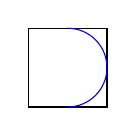
\begin{tikzpicture}
    \draw (0, 0) rectangle (1, 1);
    \draw[blue] (\xxx,\yyy+\hhh) arc(90:-90:\hhh);
  \end{tikzpicture}}

\title{Informative Selection and Spatial Process}
\date{}
\author{Bonnery,  Pantalone, Ranalli}
\begin{document}
\normalem %delete this line when ulem packages is removed

\maketitle

\tableofcontents

\begin{abstract}
This paper extends the concept of informative selection, population distribution and sample distribution in a spatial process context.
Those notions were defined by 
\cite{pfefferman_1992} in a context where the output of the random process of interest consists of independent and identically distributed realisations for each individuals of a population. \cite{BonneryBreidtCoquet} showed that informative selection was inducing a stochastic dependence among realisations on the selected units. In the context of spatial process, the "population" is a continuous space and realisations for two different elements of the population are not independent. We show how informative selection may induce a different dependence among selected units, how the sample distribution differs from the "population" distribution, and how one can  account for this effect in an simulated study when doing statistical inference, including Semi-variogram parametric and semi parametric estimation, as well as prediction on the part of the space for which the random process was not observed.
\end{abstract}

{\color{red} The references in abstracts should be either written in full or not given}.

\section{Intro}


\section{Statistical Framework} \label{sec:stat_fra}
\subsection{Spatial process}
In this paper, all random variables are defined on a probability space $(\Omega,\mathscr{A},P)$. The expected value and variance/covariance operators are defined with respect to the probability measure $P$. 
We consider a space $\Pop$, that is a subset of a finite dimensional real vector space $\mathbb{R}^d$, and a random process $\Signal$ defined on $\Pop$ with value in another finite dimension real vector space $\SignalSpace$, e.g. $Y:\Omega\to(\Pop\to\SignalSpace)$.
The notation "$g:E\to F$" means: let $g$ be a mapping from set $E$ to set $F$. For $f:E\to (F\to G)$, $g:E\to F$,  the notation $f[g]$ designates the function :  $f[g]:E\to G$, such that $f[g](x)=(f(x))(g(x))$. For example for a random variable $X:\Omega\to\Pop$, $\Signal[X]$ is the random variable: $\Omega\to\SignalSpace$, $\omega\mapsto(\Signal(\omega))(X(\omega))$.
%Given data $(\position_{1},\signal_{1}),...,(\position_{n},\signal_{n})$, in order to perform inference for some target, we postulate a model, which we assume holds for the entire population. In particular, we are interested in model parameters, in other words we focus on \emph{analytic inference}. The choice of the model is not an easy task. It should reflect the structure of the population and should capture the important features useful for inference purpose. An entire branch of literature is dedicated to this task, i.e. \emph{model selection}, but the focus of this paper does not lie in that. 
%For our work we assume that the model describing the variable of interest is given by
%\begin{equation} \label{eq:model}
%\Signal\left[\position\right]=S\left[\position\right]+\epsilon\left[\position\right]
%\end{equation}
%{\color{red} S is for $\Sample$ (sample)}
%where $S\left(\position\right)$ is a zero mean stationary stochastic process in $\mathbb{R}^d$ and is independent from the $\epsilon\left(\position\right)$, which has normal distribution with mean 0 and variance $\sigma_{\epsilon}$. The model in \eqref{eq:model} is quite general and embraces many variations under its umbrella. It is wide known in the field of geostatistics, where the term \emph{kriging} is in vogue. In fact, according to different assumptions about $S(\position)$, we end up with different models, which are usually referred with terms as ordinary kriging, simple kriging, universal kriging and so on. In order to perform inference about the model parameters, we need to introduce some assumptions.
Let $\dominantY$ (resp. $\dominantU$) denote a sigma-finite measure on the set $\SignalSpace$ (resp. $\Pop$).
The notation $\density_{V\mid W}$ denotes the density of $V$ conditional on $W$ with respect to a to be specified dominating measure on the codomain of $V$.
The average theoretical semivariogram is defined as the function $$\Semivariogram:\mathbb{R}^d\to[0,+\infty),h\mapsto\frac12\int_{\Pop^2} \Var\left[\Signal[\position_2]-\Signal[\position_1]\right] \derive(\dominantU^{\otimes 2})^{(X_1,X_2)\mid X_2-X_1=h}(\position_1,\position_2),$$
{\color{red} We need to put a reference on this formula. We jsut replace $E[^2]$ by $V$ and need to make the assumption that E[Y[x]] is constant clear in examples.}
where $(X_1,X_2)$ is the identity of $\Pop^{2}$, and the average theoretical covariogram is the function  $\nu^{X_2-X_1}-a.s(h)$-defined:
$$\Covariogram:\mathbb{R}^d\to\mathbb{R}, h\mapsto\int_{\Pop^2} \Cov\left[\Signal[\position_1],\Signal[\position_2]\right] \derive(\dominantU^{\otimes 2})^{(X_1,X_2)\mid X_2-X_1=h}(\position_1,\position_2).$$ The covariogram and semivariogram satisfy the relationship: $\forall h\in\mathbb{R}^d, \Semivariogram(h)=\Covariogram(0)-\Covariogram(h)$.

{\color{red}We will remove it later but it is handy to write it there for the moment. $$\Covariogram(h)=\Covariogram(0)-\Semivariogram(h)$$.}

\begin{definition}[Intrinsic stationarity]
A process is intrinsic stationary when the following conditions are satisfied:  $\forall \position_1,\position_2\in\Pop$,
\begin{eqnarray}
    \mathrm{E}\left[\Signal\left[\position_2\right]-\Signal\left[\position_1\right]\right]&=&0\\
    \frac12~\Var\left[\Signal\left[\position_2\right]-\Signal\left[\position_1\right]\right]&=&\Semivariogram(\position_2-\position_1)\label{eq:semivariogram}
\end{eqnarray}


%The function $\Semivariogram$ in equation \eqref{eq:semivariogram} is referred as the (theoretical) semi-variogram of the random process $\Signal$.
\end{definition}


\begin{definition}[Second order stationarity]
A process is second order stationary when the following are satisfied:
\begin{equation}
    E\left[\Signal\left[\position\right]\right]=\mu,\forall\position\in \Pop
\end{equation}
\begin{equation} \label{eq:covariogram}
    \Cov\left[\Signal\left[\position_{1}\right],\Signal\left[\position_{2}\right]\right]=C\left(\position_{1}-\position_{2}\right),\forall\position_{1},\position_{2}\in \Pop
\end{equation}
\end{definition}
%The function $\Covariogram\left(\cdot\right)$ in \eqref{eq:covariogram} is called \emph{covariogram}, or \emph{stationary covariance function}. 
The random process is isotropic if in addition on being stationary, the covaiogram function $h\mapsto \Covariogram(h)$ only depends on $h$ via $h\mapsto\|h\|$.

%{\color{red} Let us call $\gamma$ the parameters for the Semivariogram or $c$ the parameters for the Covariance.
%A plot of the 4 variograms would be neat there. Throughout the paper, $c_0$ should be replaced by $\sigma$}

Common model assumptions on the process $\Signal$ consist in assuming second order stationarity and isotropy. Covariance structure of the signal is then fully characterized by $\Covariogram(0)$ $\Semivariogram(h), h\neq 0$. We give the semi-variogram formal expression for a list of semivariogram models (See \cite{chiles1999geostatistics} for more models). For $h\in\mathbb{R}^d$, $\|h\|>0$:

\begin{table}[H]
\setlength{\tabcolsep}{28pt}
\renewcommand{\arraystretch}{1.8}
\begin{tabular}{lll}
\hline
($\Semivariogram\left(h\right)$)&Parameters&Type\\
\hline
\hline
$c_{0}+c_1\|h\|$& $c_0,~c_1\in[0,+\infty)$&Linear\\
%\hline$\begin{array}{ll}c_{0}+c_{s}\lbrace\left(3/2\right)\left(h/a_{s}\right)-\left(1/2\right)\left(h/a_{s}\right)^{3}& \text{ if } 0<h\leq a_{s},\\
%    c_{0}+c_{s}&\text{ if } h\geq a_{s}\end{array}$&&
% Spherical\\
\hline    $c_0+c_1\left( 1-\exp\left(-\|h\|/c_2\right)\right)$&$c_0,~c_1,~ c_2\in[0,+\infty)$&Exponential\\
\hline
$c_0+c_1\left(1-\exp\left(-\frac{\|h\|^2}{2c_2^2}\right)\right)$&$c_0,~c_1,~ c_2\in[0,+\infty)$&Gaussian\\
\hline
\end{tabular}
\caption{Covariograms}
\end{table}

%If $\gamma$ is continuous in $0$, $\gamma(0)=0$
\subsubsection*{Example: Gaussian processes}
In the case where $\Signal:\Omega\to(\Pop\to\SignalSpace)$ is a   Gaussian random process, its distribution  can be derived from the distributions of $\Signal[\position]$, where $\position$, of the form $\position=(\position_\ell)_{\ell\in \Sampleindex}\in\Pop^\Sampleindex$, is a vector of elements of $\Pop$ indexed by a finite set $\Sampleindex$, and where $Y[\position]$ denotes the vector of random variables $(Y[\position_\ell])_{\ell\in \Sampleindex}$. 
For $n,m\in\mathbb{N}$, $\position\in\Pop^n$, $\position'\in\Pop^m$, define the expected value of the signal as $\mu:\Pop\to\SignalSpace,\position\mapsto\mathrm{E}\left[\Signal[\position]\right]$, and the covariance matrix of the signal between points $\position_1,\ldots,\position_n$ and $\position'_1,\ldots,\position'_m$: $\provar_{\position,\position';\parampop}=\Cov \left[\Signal[\position],\Signal[\position']\right]$.
The distribution of $\Signal$ is then fully characterized by $\mu$ and $\provar$: for $n\in\mathbb{N}$,   $\position\in\Pop^n$, $\Signal[\position]$ has the following density with respect to $\dominantY^{\otimes n}$: 
%As first example, we present a spatial Gaussian process. A \emph{Gaussian process} is a stochastic process, such that every finite collection of those random variables has a multivariate normal distribution. Hence, given the model \eqref{eq:model}, we assume 
%$\Signal\sim\mathcal{N}\left(0,\provar\right)$. In this scenario the probability density function is given by: for $n\in\mathbb{N}$, $\position\in\Pop^n$,  
\begin{equation} \label{eq:pdf_norm_process}
    \density_{\Signal[\position]}\left(\signal\right)=\left(2\pi^{n/2}|\provar_{\position,\position}|^{\frac12}\right)^{-1}\exp\left(-\frac12(\signal-\mu(\position))\provar_{\position,\position}^{-1}(\signal-\mu(\position))^{\!\mathrm{T}}\right).
\end{equation}
%and the respective likelihood for a sample of dimension $n$ is
%\begin{equation} \label{lik_norm_process}
%   \mathcal{L}_{\Signal[\position]}\left(\parampop;\signal\right)=\density_{\left(\Signal\left[\position\right];\theta\right)}\left(\signal;\theta\right)
%\end{equation}
%% Created by tikzDevice version 0.12 on 2019-06-03 14:32:54
% !TEX encoding = UTF-8 Unicode
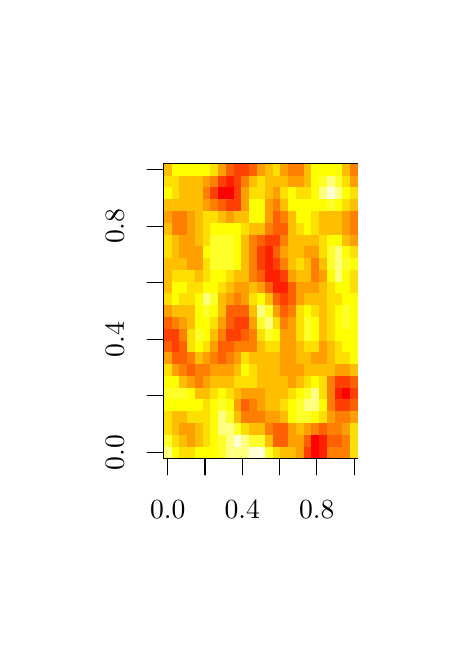
\begin{tikzpicture}[x=1pt,y=1pt]
\definecolor{fillColor}{RGB}{255,255,255}
\path[use as bounding box,fill=fillColor,fill opacity=0.00] (0,0) rectangle (144.54,216.81);
\begin{scope}
\path[clip] (  0.00,  0.00) rectangle (144.54,216.81);
\definecolor{drawColor}{RGB}{0,0,0}

\path[draw=drawColor,line width= 0.4pt,line join=round,line cap=round] ( 50.60, 61.20) -- (117.94, 61.20);

\path[draw=drawColor,line width= 0.4pt,line join=round,line cap=round] ( 50.60, 61.20) -- ( 50.60, 55.20);

\path[draw=drawColor,line width= 0.4pt,line join=round,line cap=round] ( 64.07, 61.20) -- ( 64.07, 55.20);

\path[draw=drawColor,line width= 0.4pt,line join=round,line cap=round] ( 77.54, 61.20) -- ( 77.54, 55.20);

\path[draw=drawColor,line width= 0.4pt,line join=round,line cap=round] ( 91.00, 61.20) -- ( 91.00, 55.20);

\path[draw=drawColor,line width= 0.4pt,line join=round,line cap=round] (104.47, 61.20) -- (104.47, 55.20);

\path[draw=drawColor,line width= 0.4pt,line join=round,line cap=round] (117.94, 61.20) -- (117.94, 55.20);

\node[text=drawColor,anchor=base,inner sep=0pt, outer sep=0pt, scale=  1.00] at ( 50.60, 39.60) {0.0};

\node[text=drawColor,anchor=base,inner sep=0pt, outer sep=0pt, scale=  1.00] at ( 77.54, 39.60) {0.4};

\node[text=drawColor,anchor=base,inner sep=0pt, outer sep=0pt, scale=  1.00] at (104.47, 39.60) {0.8};

\path[draw=drawColor,line width= 0.4pt,line join=round,line cap=round] ( 49.20, 63.33) -- ( 49.20,165.48);

\path[draw=drawColor,line width= 0.4pt,line join=round,line cap=round] ( 49.20, 63.33) -- ( 43.20, 63.33);

\path[draw=drawColor,line width= 0.4pt,line join=round,line cap=round] ( 49.20, 83.76) -- ( 43.20, 83.76);

\path[draw=drawColor,line width= 0.4pt,line join=round,line cap=round] ( 49.20,104.19) -- ( 43.20,104.19);

\path[draw=drawColor,line width= 0.4pt,line join=round,line cap=round] ( 49.20,124.62) -- ( 43.20,124.62);

\path[draw=drawColor,line width= 0.4pt,line join=round,line cap=round] ( 49.20,145.05) -- ( 43.20,145.05);

\path[draw=drawColor,line width= 0.4pt,line join=round,line cap=round] ( 49.20,165.48) -- ( 43.20,165.48);

\node[text=drawColor,rotate= 90.00,anchor=base,inner sep=0pt, outer sep=0pt, scale=  1.00] at ( 34.80, 63.33) {0.0};

\node[text=drawColor,rotate= 90.00,anchor=base,inner sep=0pt, outer sep=0pt, scale=  1.00] at ( 34.80,104.19) {0.4};

\node[text=drawColor,rotate= 90.00,anchor=base,inner sep=0pt, outer sep=0pt, scale=  1.00] at ( 34.80,145.05) {0.8};

\path[draw=drawColor,line width= 0.4pt,line join=round,line cap=round] ( 49.20, 61.20) --
	(119.34, 61.20) --
	(119.34,167.61) --
	( 49.20,167.61) --
	( 49.20, 61.20);
\end{scope}
\begin{scope}
\path[clip] ( 49.20, 61.20) rectangle (119.34,167.61);
\definecolor{fillColor}{RGB}{255,255,128}

\path[fill=fillColor] ( 49.20, 61.20) rectangle ( 52.01, 65.46);
\definecolor{fillColor}{RGB}{255,255,42}

\path[fill=fillColor] ( 49.20, 65.46) rectangle ( 52.01, 69.71);
\definecolor{fillColor}{RGB}{255,223,0}

\path[fill=fillColor] ( 49.20, 69.71) rectangle ( 52.01, 73.97);

\path[fill=fillColor] ( 49.20, 73.97) rectangle ( 52.01, 78.23);
\definecolor{fillColor}{RGB}{255,255,0}

\path[fill=fillColor] ( 49.20, 78.23) rectangle ( 52.01, 82.48);
\definecolor{fillColor}{RGB}{255,255,42}

\path[fill=fillColor] ( 49.20, 82.48) rectangle ( 52.01, 86.74);
\definecolor{fillColor}{RGB}{255,255,0}

\path[fill=fillColor] ( 49.20, 86.74) rectangle ( 52.01, 90.99);
\definecolor{fillColor}{RGB}{255,223,0}

\path[fill=fillColor] ( 49.20, 90.99) rectangle ( 52.01, 95.25);
\definecolor{fillColor}{RGB}{255,159,0}

\path[fill=fillColor] ( 49.20, 95.25) rectangle ( 52.01, 99.51);
\definecolor{fillColor}{RGB}{255,96,0}

\path[fill=fillColor] ( 49.20, 99.51) rectangle ( 52.01,103.76);
\definecolor{fillColor}{RGB}{255,64,0}

\path[fill=fillColor] ( 49.20,103.76) rectangle ( 52.01,108.02);
\definecolor{fillColor}{RGB}{255,96,0}

\path[fill=fillColor] ( 49.20,108.02) rectangle ( 52.01,112.28);
\definecolor{fillColor}{RGB}{255,159,0}

\path[fill=fillColor] ( 49.20,112.28) rectangle ( 52.01,116.53);
\definecolor{fillColor}{RGB}{255,223,0}

\path[fill=fillColor] ( 49.20,116.53) rectangle ( 52.01,120.79);
\definecolor{fillColor}{RGB}{255,191,0}

\path[fill=fillColor] ( 49.20,120.79) rectangle ( 52.01,125.05);

\path[fill=fillColor] ( 49.20,125.05) rectangle ( 52.01,129.30);

\path[fill=fillColor] ( 49.20,129.30) rectangle ( 52.01,133.56);
\definecolor{fillColor}{RGB}{255,223,0}

\path[fill=fillColor] ( 49.20,133.56) rectangle ( 52.01,137.82);

\path[fill=fillColor] ( 49.20,137.82) rectangle ( 52.01,142.07);
\definecolor{fillColor}{RGB}{255,191,0}

\path[fill=fillColor] ( 49.20,142.07) rectangle ( 52.01,146.33);
\definecolor{fillColor}{RGB}{255,159,0}

\path[fill=fillColor] ( 49.20,146.33) rectangle ( 52.01,150.58);
\definecolor{fillColor}{RGB}{255,191,0}

\path[fill=fillColor] ( 49.20,150.58) rectangle ( 52.01,154.84);
\definecolor{fillColor}{RGB}{255,255,0}

\path[fill=fillColor] ( 49.20,154.84) rectangle ( 52.01,159.10);
\definecolor{fillColor}{RGB}{255,223,0}

\path[fill=fillColor] ( 49.20,159.10) rectangle ( 52.01,163.35);
\definecolor{fillColor}{RGB}{255,191,0}

\path[fill=fillColor] ( 49.20,163.35) rectangle ( 52.01,167.61);
\definecolor{fillColor}{RGB}{255,255,0}

\path[fill=fillColor] ( 52.01, 61.20) rectangle ( 54.81, 65.46);
\definecolor{fillColor}{RGB}{255,223,0}

\path[fill=fillColor] ( 52.01, 65.46) rectangle ( 54.81, 69.71);
\definecolor{fillColor}{RGB}{255,191,0}

\path[fill=fillColor] ( 52.01, 69.71) rectangle ( 54.81, 73.97);

\path[fill=fillColor] ( 52.01, 73.97) rectangle ( 54.81, 78.23);
\definecolor{fillColor}{RGB}{255,255,0}

\path[fill=fillColor] ( 52.01, 78.23) rectangle ( 54.81, 82.48);
\definecolor{fillColor}{RGB}{255,255,42}

\path[fill=fillColor] ( 52.01, 82.48) rectangle ( 54.81, 86.74);
\definecolor{fillColor}{RGB}{255,255,0}

\path[fill=fillColor] ( 52.01, 86.74) rectangle ( 54.81, 90.99);
\definecolor{fillColor}{RGB}{255,159,0}

\path[fill=fillColor] ( 52.01, 90.99) rectangle ( 54.81, 95.25);
\definecolor{fillColor}{RGB}{255,96,0}

\path[fill=fillColor] ( 52.01, 95.25) rectangle ( 54.81, 99.51);
\definecolor{fillColor}{RGB}{255,64,0}

\path[fill=fillColor] ( 52.01, 99.51) rectangle ( 54.81,103.76);

\path[fill=fillColor] ( 52.01,103.76) rectangle ( 54.81,108.02);
\definecolor{fillColor}{RGB}{255,128,0}

\path[fill=fillColor] ( 52.01,108.02) rectangle ( 54.81,112.28);
\definecolor{fillColor}{RGB}{255,191,0}

\path[fill=fillColor] ( 52.01,112.28) rectangle ( 54.81,116.53);
\definecolor{fillColor}{RGB}{255,255,0}

\path[fill=fillColor] ( 52.01,116.53) rectangle ( 54.81,120.79);

\path[fill=fillColor] ( 52.01,120.79) rectangle ( 54.81,125.05);
\definecolor{fillColor}{RGB}{255,223,0}

\path[fill=fillColor] ( 52.01,125.05) rectangle ( 54.81,129.30);
\definecolor{fillColor}{RGB}{255,191,0}

\path[fill=fillColor] ( 52.01,129.30) rectangle ( 54.81,133.56);

\path[fill=fillColor] ( 52.01,133.56) rectangle ( 54.81,137.82);

\path[fill=fillColor] ( 52.01,137.82) rectangle ( 54.81,142.07);
\definecolor{fillColor}{RGB}{255,128,0}

\path[fill=fillColor] ( 52.01,142.07) rectangle ( 54.81,146.33);

\path[fill=fillColor] ( 52.01,146.33) rectangle ( 54.81,150.58);
\definecolor{fillColor}{RGB}{255,191,0}

\path[fill=fillColor] ( 52.01,150.58) rectangle ( 54.81,154.84);
\definecolor{fillColor}{RGB}{255,223,0}

\path[fill=fillColor] ( 52.01,154.84) rectangle ( 54.81,159.10);

\path[fill=fillColor] ( 52.01,159.10) rectangle ( 54.81,163.35);
\definecolor{fillColor}{RGB}{255,255,0}

\path[fill=fillColor] ( 52.01,163.35) rectangle ( 54.81,167.61);
\definecolor{fillColor}{RGB}{255,223,0}

\path[fill=fillColor] ( 54.81, 61.20) rectangle ( 57.62, 65.46);
\definecolor{fillColor}{RGB}{255,191,0}

\path[fill=fillColor] ( 54.81, 65.46) rectangle ( 57.62, 69.71);
\definecolor{fillColor}{RGB}{255,159,0}

\path[fill=fillColor] ( 54.81, 69.71) rectangle ( 57.62, 73.97);
\definecolor{fillColor}{RGB}{255,191,0}

\path[fill=fillColor] ( 54.81, 73.97) rectangle ( 57.62, 78.23);
\definecolor{fillColor}{RGB}{255,255,0}

\path[fill=fillColor] ( 54.81, 78.23) rectangle ( 57.62, 82.48);
\definecolor{fillColor}{RGB}{255,255,42}

\path[fill=fillColor] ( 54.81, 82.48) rectangle ( 57.62, 86.74);
\definecolor{fillColor}{RGB}{255,191,0}

\path[fill=fillColor] ( 54.81, 86.74) rectangle ( 57.62, 90.99);
\definecolor{fillColor}{RGB}{255,128,0}

\path[fill=fillColor] ( 54.81, 90.99) rectangle ( 57.62, 95.25);
\definecolor{fillColor}{RGB}{255,96,0}

\path[fill=fillColor] ( 54.81, 95.25) rectangle ( 57.62, 99.51);

\path[fill=fillColor] ( 54.81, 99.51) rectangle ( 57.62,103.76);
\definecolor{fillColor}{RGB}{255,128,0}

\path[fill=fillColor] ( 54.81,103.76) rectangle ( 57.62,108.02);
\definecolor{fillColor}{RGB}{255,159,0}

\path[fill=fillColor] ( 54.81,108.02) rectangle ( 57.62,112.28);
\definecolor{fillColor}{RGB}{255,191,0}

\path[fill=fillColor] ( 54.81,112.28) rectangle ( 57.62,116.53);
\definecolor{fillColor}{RGB}{255,223,0}

\path[fill=fillColor] ( 54.81,116.53) rectangle ( 57.62,120.79);
\definecolor{fillColor}{RGB}{255,255,0}

\path[fill=fillColor] ( 54.81,120.79) rectangle ( 57.62,125.05);
\definecolor{fillColor}{RGB}{255,223,0}

\path[fill=fillColor] ( 54.81,125.05) rectangle ( 57.62,129.30);
\definecolor{fillColor}{RGB}{255,191,0}

\path[fill=fillColor] ( 54.81,129.30) rectangle ( 57.62,133.56);
\definecolor{fillColor}{RGB}{255,159,0}

\path[fill=fillColor] ( 54.81,133.56) rectangle ( 57.62,137.82);

\path[fill=fillColor] ( 54.81,137.82) rectangle ( 57.62,142.07);
\definecolor{fillColor}{RGB}{255,128,0}

\path[fill=fillColor] ( 54.81,142.07) rectangle ( 57.62,146.33);

\path[fill=fillColor] ( 54.81,146.33) rectangle ( 57.62,150.58);
\definecolor{fillColor}{RGB}{255,191,0}

\path[fill=fillColor] ( 54.81,150.58) rectangle ( 57.62,154.84);

\path[fill=fillColor] ( 54.81,154.84) rectangle ( 57.62,159.10);

\path[fill=fillColor] ( 54.81,159.10) rectangle ( 57.62,163.35);
\definecolor{fillColor}{RGB}{255,255,0}

\path[fill=fillColor] ( 54.81,163.35) rectangle ( 57.62,167.61);
\definecolor{fillColor}{RGB}{255,223,0}

\path[fill=fillColor] ( 57.62, 61.20) rectangle ( 60.42, 65.46);
\definecolor{fillColor}{RGB}{255,159,0}

\path[fill=fillColor] ( 57.62, 65.46) rectangle ( 60.42, 69.71);

\path[fill=fillColor] ( 57.62, 69.71) rectangle ( 60.42, 73.97);
\definecolor{fillColor}{RGB}{255,223,0}

\path[fill=fillColor] ( 57.62, 73.97) rectangle ( 60.42, 78.23);
\definecolor{fillColor}{RGB}{255,255,0}

\path[fill=fillColor] ( 57.62, 78.23) rectangle ( 60.42, 82.48);

\path[fill=fillColor] ( 57.62, 82.48) rectangle ( 60.42, 86.74);
\definecolor{fillColor}{RGB}{255,159,0}

\path[fill=fillColor] ( 57.62, 86.74) rectangle ( 60.42, 90.99);
\definecolor{fillColor}{RGB}{255,96,0}

\path[fill=fillColor] ( 57.62, 90.99) rectangle ( 60.42, 95.25);
\definecolor{fillColor}{RGB}{255,128,0}

\path[fill=fillColor] ( 57.62, 95.25) rectangle ( 60.42, 99.51);
\definecolor{fillColor}{RGB}{255,223,0}

\path[fill=fillColor] ( 57.62, 99.51) rectangle ( 60.42,103.76);

\path[fill=fillColor] ( 57.62,103.76) rectangle ( 60.42,108.02);
\definecolor{fillColor}{RGB}{255,191,0}

\path[fill=fillColor] ( 57.62,108.02) rectangle ( 60.42,112.28);

\path[fill=fillColor] ( 57.62,112.28) rectangle ( 60.42,116.53);
\definecolor{fillColor}{RGB}{255,223,0}

\path[fill=fillColor] ( 57.62,116.53) rectangle ( 60.42,120.79);

\path[fill=fillColor] ( 57.62,120.79) rectangle ( 60.42,125.05);

\path[fill=fillColor] ( 57.62,125.05) rectangle ( 60.42,129.30);
\definecolor{fillColor}{RGB}{255,159,0}

\path[fill=fillColor] ( 57.62,129.30) rectangle ( 60.42,133.56);

\path[fill=fillColor] ( 57.62,133.56) rectangle ( 60.42,137.82);

\path[fill=fillColor] ( 57.62,137.82) rectangle ( 60.42,142.07);

\path[fill=fillColor] ( 57.62,142.07) rectangle ( 60.42,146.33);

\path[fill=fillColor] ( 57.62,146.33) rectangle ( 60.42,150.58);
\definecolor{fillColor}{RGB}{255,191,0}

\path[fill=fillColor] ( 57.62,150.58) rectangle ( 60.42,154.84);

\path[fill=fillColor] ( 57.62,154.84) rectangle ( 60.42,159.10);

\path[fill=fillColor] ( 57.62,159.10) rectangle ( 60.42,163.35);
\definecolor{fillColor}{RGB}{255,255,0}

\path[fill=fillColor] ( 57.62,163.35) rectangle ( 60.42,167.61);

\path[fill=fillColor] ( 60.42, 61.20) rectangle ( 63.23, 65.46);
\definecolor{fillColor}{RGB}{255,191,0}

\path[fill=fillColor] ( 60.42, 65.46) rectangle ( 63.23, 69.71);

\path[fill=fillColor] ( 60.42, 69.71) rectangle ( 63.23, 73.97);
\definecolor{fillColor}{RGB}{255,223,0}

\path[fill=fillColor] ( 60.42, 73.97) rectangle ( 63.23, 78.23);
\definecolor{fillColor}{RGB}{255,255,0}

\path[fill=fillColor] ( 60.42, 78.23) rectangle ( 63.23, 82.48);
\definecolor{fillColor}{RGB}{255,191,0}

\path[fill=fillColor] ( 60.42, 82.48) rectangle ( 63.23, 86.74);
\definecolor{fillColor}{RGB}{255,128,0}

\path[fill=fillColor] ( 60.42, 86.74) rectangle ( 63.23, 90.99);

\path[fill=fillColor] ( 60.42, 90.99) rectangle ( 63.23, 95.25);
\definecolor{fillColor}{RGB}{255,191,0}

\path[fill=fillColor] ( 60.42, 95.25) rectangle ( 63.23, 99.51);
\definecolor{fillColor}{RGB}{255,255,0}

\path[fill=fillColor] ( 60.42, 99.51) rectangle ( 63.23,103.76);
\definecolor{fillColor}{RGB}{255,255,42}

\path[fill=fillColor] ( 60.42,103.76) rectangle ( 63.23,108.02);
\definecolor{fillColor}{RGB}{255,255,0}

\path[fill=fillColor] ( 60.42,108.02) rectangle ( 63.23,112.28);

\path[fill=fillColor] ( 60.42,112.28) rectangle ( 63.23,116.53);

\path[fill=fillColor] ( 60.42,116.53) rectangle ( 63.23,120.79);
\definecolor{fillColor}{RGB}{255,223,0}

\path[fill=fillColor] ( 60.42,120.79) rectangle ( 63.23,125.05);
\definecolor{fillColor}{RGB}{255,191,0}

\path[fill=fillColor] ( 60.42,125.05) rectangle ( 63.23,129.30);
\definecolor{fillColor}{RGB}{255,159,0}

\path[fill=fillColor] ( 60.42,129.30) rectangle ( 63.23,133.56);

\path[fill=fillColor] ( 60.42,133.56) rectangle ( 63.23,137.82);
\definecolor{fillColor}{RGB}{255,191,0}

\path[fill=fillColor] ( 60.42,137.82) rectangle ( 63.23,142.07);

\path[fill=fillColor] ( 60.42,142.07) rectangle ( 63.23,146.33);

\path[fill=fillColor] ( 60.42,146.33) rectangle ( 63.23,150.58);

\path[fill=fillColor] ( 60.42,150.58) rectangle ( 63.23,154.84);

\path[fill=fillColor] ( 60.42,154.84) rectangle ( 63.23,159.10);

\path[fill=fillColor] ( 60.42,159.10) rectangle ( 63.23,163.35);
\definecolor{fillColor}{RGB}{255,255,0}

\path[fill=fillColor] ( 60.42,163.35) rectangle ( 63.23,167.61);

\path[fill=fillColor] ( 63.23, 61.20) rectangle ( 66.03, 65.46);
\definecolor{fillColor}{RGB}{255,223,0}

\path[fill=fillColor] ( 63.23, 65.46) rectangle ( 66.03, 69.71);

\path[fill=fillColor] ( 63.23, 69.71) rectangle ( 66.03, 73.97);

\path[fill=fillColor] ( 63.23, 73.97) rectangle ( 66.03, 78.23);

\path[fill=fillColor] ( 63.23, 78.23) rectangle ( 66.03, 82.48);
\definecolor{fillColor}{RGB}{255,191,0}

\path[fill=fillColor] ( 63.23, 82.48) rectangle ( 66.03, 86.74);
\definecolor{fillColor}{RGB}{255,159,0}

\path[fill=fillColor] ( 63.23, 86.74) rectangle ( 66.03, 90.99);
\definecolor{fillColor}{RGB}{255,128,0}

\path[fill=fillColor] ( 63.23, 90.99) rectangle ( 66.03, 95.25);
\definecolor{fillColor}{RGB}{255,159,0}

\path[fill=fillColor] ( 63.23, 95.25) rectangle ( 66.03, 99.51);
\definecolor{fillColor}{RGB}{255,223,0}

\path[fill=fillColor] ( 63.23, 99.51) rectangle ( 66.03,103.76);
\definecolor{fillColor}{RGB}{255,255,0}

\path[fill=fillColor] ( 63.23,103.76) rectangle ( 66.03,108.02);

\path[fill=fillColor] ( 63.23,108.02) rectangle ( 66.03,112.28);
\definecolor{fillColor}{RGB}{255,255,42}

\path[fill=fillColor] ( 63.23,112.28) rectangle ( 66.03,116.53);
\definecolor{fillColor}{RGB}{255,255,128}

\path[fill=fillColor] ( 63.23,116.53) rectangle ( 66.03,120.79);
\definecolor{fillColor}{RGB}{255,255,0}

\path[fill=fillColor] ( 63.23,120.79) rectangle ( 66.03,125.05);
\definecolor{fillColor}{RGB}{255,223,0}

\path[fill=fillColor] ( 63.23,125.05) rectangle ( 66.03,129.30);

\path[fill=fillColor] ( 63.23,129.30) rectangle ( 66.03,133.56);
\definecolor{fillColor}{RGB}{255,255,0}

\path[fill=fillColor] ( 63.23,133.56) rectangle ( 66.03,137.82);
\definecolor{fillColor}{RGB}{255,223,0}

\path[fill=fillColor] ( 63.23,137.82) rectangle ( 66.03,142.07);

\path[fill=fillColor] ( 63.23,142.07) rectangle ( 66.03,146.33);

\path[fill=fillColor] ( 63.23,146.33) rectangle ( 66.03,150.58);
\definecolor{fillColor}{RGB}{255,159,0}

\path[fill=fillColor] ( 63.23,150.58) rectangle ( 66.03,154.84);
\definecolor{fillColor}{RGB}{255,128,0}

\path[fill=fillColor] ( 63.23,154.84) rectangle ( 66.03,159.10);
\definecolor{fillColor}{RGB}{255,159,0}

\path[fill=fillColor] ( 63.23,159.10) rectangle ( 66.03,163.35);
\definecolor{fillColor}{RGB}{255,255,0}

\path[fill=fillColor] ( 63.23,163.35) rectangle ( 66.03,167.61);

\path[fill=fillColor] ( 66.03, 61.20) rectangle ( 68.84, 65.46);

\path[fill=fillColor] ( 66.03, 65.46) rectangle ( 68.84, 69.71);

\path[fill=fillColor] ( 66.03, 69.71) rectangle ( 68.84, 73.97);

\path[fill=fillColor] ( 66.03, 73.97) rectangle ( 68.84, 78.23);

\path[fill=fillColor] ( 66.03, 78.23) rectangle ( 68.84, 82.48);
\definecolor{fillColor}{RGB}{255,223,0}

\path[fill=fillColor] ( 66.03, 82.48) rectangle ( 68.84, 86.74);
\definecolor{fillColor}{RGB}{255,191,0}

\path[fill=fillColor] ( 66.03, 86.74) rectangle ( 68.84, 90.99);
\definecolor{fillColor}{RGB}{255,159,0}

\path[fill=fillColor] ( 66.03, 90.99) rectangle ( 68.84, 95.25);
\definecolor{fillColor}{RGB}{255,128,0}

\path[fill=fillColor] ( 66.03, 95.25) rectangle ( 68.84, 99.51);
\definecolor{fillColor}{RGB}{255,159,0}

\path[fill=fillColor] ( 66.03, 99.51) rectangle ( 68.84,103.76);
\definecolor{fillColor}{RGB}{255,191,0}

\path[fill=fillColor] ( 66.03,103.76) rectangle ( 68.84,108.02);
\definecolor{fillColor}{RGB}{255,223,0}

\path[fill=fillColor] ( 66.03,108.02) rectangle ( 68.84,112.28);
\definecolor{fillColor}{RGB}{255,255,0}

\path[fill=fillColor] ( 66.03,112.28) rectangle ( 68.84,116.53);
\definecolor{fillColor}{RGB}{255,255,42}

\path[fill=fillColor] ( 66.03,116.53) rectangle ( 68.84,120.79);
\definecolor{fillColor}{RGB}{255,255,0}

\path[fill=fillColor] ( 66.03,120.79) rectangle ( 68.84,125.05);

\path[fill=fillColor] ( 66.03,125.05) rectangle ( 68.84,129.30);
\definecolor{fillColor}{RGB}{255,255,42}

\path[fill=fillColor] ( 66.03,129.30) rectangle ( 68.84,133.56);

\path[fill=fillColor] ( 66.03,133.56) rectangle ( 68.84,137.82);

\path[fill=fillColor] ( 66.03,137.82) rectangle ( 68.84,142.07);
\definecolor{fillColor}{RGB}{255,255,0}

\path[fill=fillColor] ( 66.03,142.07) rectangle ( 68.84,146.33);
\definecolor{fillColor}{RGB}{255,223,0}

\path[fill=fillColor] ( 66.03,146.33) rectangle ( 68.84,150.58);
\definecolor{fillColor}{RGB}{255,128,0}

\path[fill=fillColor] ( 66.03,150.58) rectangle ( 68.84,154.84);
\definecolor{fillColor}{RGB}{255,64,0}

\path[fill=fillColor] ( 66.03,154.84) rectangle ( 68.84,159.10);
\definecolor{fillColor}{RGB}{255,128,0}

\path[fill=fillColor] ( 66.03,159.10) rectangle ( 68.84,163.35);
\definecolor{fillColor}{RGB}{255,223,0}

\path[fill=fillColor] ( 66.03,163.35) rectangle ( 68.84,167.61);
\definecolor{fillColor}{RGB}{255,255,42}

\path[fill=fillColor] ( 68.84, 61.20) rectangle ( 71.64, 65.46);

\path[fill=fillColor] ( 68.84, 65.46) rectangle ( 71.64, 69.71);
\definecolor{fillColor}{RGB}{255,255,128}

\path[fill=fillColor] ( 68.84, 69.71) rectangle ( 71.64, 73.97);

\path[fill=fillColor] ( 68.84, 73.97) rectangle ( 71.64, 78.23);
\definecolor{fillColor}{RGB}{255,255,42}

\path[fill=fillColor] ( 68.84, 78.23) rectangle ( 71.64, 82.48);
\definecolor{fillColor}{RGB}{255,255,0}

\path[fill=fillColor] ( 68.84, 82.48) rectangle ( 71.64, 86.74);
\definecolor{fillColor}{RGB}{255,191,0}

\path[fill=fillColor] ( 68.84, 86.74) rectangle ( 71.64, 90.99);
\definecolor{fillColor}{RGB}{255,159,0}

\path[fill=fillColor] ( 68.84, 90.99) rectangle ( 71.64, 95.25);
\definecolor{fillColor}{RGB}{255,96,0}

\path[fill=fillColor] ( 68.84, 95.25) rectangle ( 71.64, 99.51);

\path[fill=fillColor] ( 68.84, 99.51) rectangle ( 71.64,103.76);
\definecolor{fillColor}{RGB}{255,128,0}

\path[fill=fillColor] ( 68.84,103.76) rectangle ( 71.64,108.02);
\definecolor{fillColor}{RGB}{255,159,0}

\path[fill=fillColor] ( 68.84,108.02) rectangle ( 71.64,112.28);
\definecolor{fillColor}{RGB}{255,191,0}

\path[fill=fillColor] ( 68.84,112.28) rectangle ( 71.64,116.53);

\path[fill=fillColor] ( 68.84,116.53) rectangle ( 71.64,120.79);
\definecolor{fillColor}{RGB}{255,223,0}

\path[fill=fillColor] ( 68.84,120.79) rectangle ( 71.64,125.05);
\definecolor{fillColor}{RGB}{255,255,0}

\path[fill=fillColor] ( 68.84,125.05) rectangle ( 71.64,129.30);
\definecolor{fillColor}{RGB}{255,255,42}

\path[fill=fillColor] ( 68.84,129.30) rectangle ( 71.64,133.56);

\path[fill=fillColor] ( 68.84,133.56) rectangle ( 71.64,137.82);

\path[fill=fillColor] ( 68.84,137.82) rectangle ( 71.64,142.07);
\definecolor{fillColor}{RGB}{255,255,0}

\path[fill=fillColor] ( 68.84,142.07) rectangle ( 71.64,146.33);
\definecolor{fillColor}{RGB}{255,191,0}

\path[fill=fillColor] ( 68.84,146.33) rectangle ( 71.64,150.58);
\definecolor{fillColor}{RGB}{255,96,0}

\path[fill=fillColor] ( 68.84,150.58) rectangle ( 71.64,154.84);
\definecolor{fillColor}{RGB}{255,0,0}

\path[fill=fillColor] ( 68.84,154.84) rectangle ( 71.64,159.10);
\definecolor{fillColor}{RGB}{255,64,0}

\path[fill=fillColor] ( 68.84,159.10) rectangle ( 71.64,163.35);
\definecolor{fillColor}{RGB}{255,159,0}

\path[fill=fillColor] ( 68.84,163.35) rectangle ( 71.64,167.61);
\definecolor{fillColor}{RGB}{255,255,128}

\path[fill=fillColor] ( 71.64, 61.20) rectangle ( 74.45, 65.46);

\path[fill=fillColor] ( 71.64, 65.46) rectangle ( 74.45, 69.71);

\path[fill=fillColor] ( 71.64, 69.71) rectangle ( 74.45, 73.97);
\definecolor{fillColor}{RGB}{255,255,42}

\path[fill=fillColor] ( 71.64, 73.97) rectangle ( 74.45, 78.23);
\definecolor{fillColor}{RGB}{255,255,0}

\path[fill=fillColor] ( 71.64, 78.23) rectangle ( 74.45, 82.48);
\definecolor{fillColor}{RGB}{255,223,0}

\path[fill=fillColor] ( 71.64, 82.48) rectangle ( 74.45, 86.74);
\definecolor{fillColor}{RGB}{255,191,0}

\path[fill=fillColor] ( 71.64, 86.74) rectangle ( 74.45, 90.99);
\definecolor{fillColor}{RGB}{255,159,0}

\path[fill=fillColor] ( 71.64, 90.99) rectangle ( 74.45, 95.25);
\definecolor{fillColor}{RGB}{255,128,0}

\path[fill=fillColor] ( 71.64, 95.25) rectangle ( 74.45, 99.51);
\definecolor{fillColor}{RGB}{255,96,0}

\path[fill=fillColor] ( 71.64, 99.51) rectangle ( 74.45,103.76);
\definecolor{fillColor}{RGB}{255,64,0}

\path[fill=fillColor] ( 71.64,103.76) rectangle ( 74.45,108.02);
\definecolor{fillColor}{RGB}{255,96,0}

\path[fill=fillColor] ( 71.64,108.02) rectangle ( 74.45,112.28);

\path[fill=fillColor] ( 71.64,112.28) rectangle ( 74.45,116.53);
\definecolor{fillColor}{RGB}{255,159,0}

\path[fill=fillColor] ( 71.64,116.53) rectangle ( 74.45,120.79);
\definecolor{fillColor}{RGB}{255,191,0}

\path[fill=fillColor] ( 71.64,120.79) rectangle ( 74.45,125.05);
\definecolor{fillColor}{RGB}{255,223,0}

\path[fill=fillColor] ( 71.64,125.05) rectangle ( 74.45,129.30);
\definecolor{fillColor}{RGB}{255,255,42}

\path[fill=fillColor] ( 71.64,129.30) rectangle ( 74.45,133.56);

\path[fill=fillColor] ( 71.64,133.56) rectangle ( 74.45,137.82);

\path[fill=fillColor] ( 71.64,137.82) rectangle ( 74.45,142.07);
\definecolor{fillColor}{RGB}{255,255,0}

\path[fill=fillColor] ( 71.64,142.07) rectangle ( 74.45,146.33);
\definecolor{fillColor}{RGB}{255,159,0}

\path[fill=fillColor] ( 71.64,146.33) rectangle ( 74.45,150.58);
\definecolor{fillColor}{RGB}{255,64,0}

\path[fill=fillColor] ( 71.64,150.58) rectangle ( 74.45,154.84);
\definecolor{fillColor}{RGB}{255,0,0}

\path[fill=fillColor] ( 71.64,154.84) rectangle ( 74.45,159.10);
\definecolor{fillColor}{RGB}{255,32,0}

\path[fill=fillColor] ( 71.64,159.10) rectangle ( 74.45,163.35);
\definecolor{fillColor}{RGB}{255,96,0}

\path[fill=fillColor] ( 71.64,163.35) rectangle ( 74.45,167.61);
\definecolor{fillColor}{RGB}{255,255,128}

\path[fill=fillColor] ( 74.45, 61.20) rectangle ( 77.26, 65.46);
\definecolor{fillColor}{RGB}{255,255,213}

\path[fill=fillColor] ( 74.45, 65.46) rectangle ( 77.26, 69.71);
\definecolor{fillColor}{RGB}{255,255,42}

\path[fill=fillColor] ( 74.45, 69.71) rectangle ( 77.26, 73.97);
\definecolor{fillColor}{RGB}{255,191,0}

\path[fill=fillColor] ( 74.45, 73.97) rectangle ( 77.26, 78.23);
\definecolor{fillColor}{RGB}{255,159,0}

\path[fill=fillColor] ( 74.45, 78.23) rectangle ( 77.26, 82.48);
\definecolor{fillColor}{RGB}{255,191,0}

\path[fill=fillColor] ( 74.45, 82.48) rectangle ( 77.26, 86.74);
\definecolor{fillColor}{RGB}{255,223,0}

\path[fill=fillColor] ( 74.45, 86.74) rectangle ( 77.26, 90.99);
\definecolor{fillColor}{RGB}{255,191,0}

\path[fill=fillColor] ( 74.45, 90.99) rectangle ( 77.26, 95.25);
\definecolor{fillColor}{RGB}{255,159,0}

\path[fill=fillColor] ( 74.45, 95.25) rectangle ( 77.26, 99.51);
\definecolor{fillColor}{RGB}{255,128,0}

\path[fill=fillColor] ( 74.45, 99.51) rectangle ( 77.26,103.76);
\definecolor{fillColor}{RGB}{255,64,0}

\path[fill=fillColor] ( 74.45,103.76) rectangle ( 77.26,108.02);

\path[fill=fillColor] ( 74.45,108.02) rectangle ( 77.26,112.28);
\definecolor{fillColor}{RGB}{255,96,0}

\path[fill=fillColor] ( 74.45,112.28) rectangle ( 77.26,116.53);
\definecolor{fillColor}{RGB}{255,128,0}

\path[fill=fillColor] ( 74.45,116.53) rectangle ( 77.26,120.79);
\definecolor{fillColor}{RGB}{255,159,0}

\path[fill=fillColor] ( 74.45,120.79) rectangle ( 77.26,125.05);
\definecolor{fillColor}{RGB}{255,191,0}

\path[fill=fillColor] ( 74.45,125.05) rectangle ( 77.26,129.30);
\definecolor{fillColor}{RGB}{255,255,0}

\path[fill=fillColor] ( 74.45,129.30) rectangle ( 77.26,133.56);

\path[fill=fillColor] ( 74.45,133.56) rectangle ( 77.26,137.82);

\path[fill=fillColor] ( 74.45,137.82) rectangle ( 77.26,142.07);

\path[fill=fillColor] ( 74.45,142.07) rectangle ( 77.26,146.33);
\definecolor{fillColor}{RGB}{255,191,0}

\path[fill=fillColor] ( 74.45,146.33) rectangle ( 77.26,150.58);
\definecolor{fillColor}{RGB}{255,64,0}

\path[fill=fillColor] ( 74.45,150.58) rectangle ( 77.26,154.84);

\path[fill=fillColor] ( 74.45,154.84) rectangle ( 77.26,159.10);

\path[fill=fillColor] ( 74.45,159.10) rectangle ( 77.26,163.35);

\path[fill=fillColor] ( 74.45,163.35) rectangle ( 77.26,167.61);
\definecolor{fillColor}{RGB}{255,255,128}

\path[fill=fillColor] ( 77.26, 61.20) rectangle ( 80.06, 65.46);

\path[fill=fillColor] ( 77.26, 65.46) rectangle ( 80.06, 69.71);
\definecolor{fillColor}{RGB}{255,223,0}

\path[fill=fillColor] ( 77.26, 69.71) rectangle ( 80.06, 73.97);
\definecolor{fillColor}{RGB}{255,128,0}

\path[fill=fillColor] ( 77.26, 73.97) rectangle ( 80.06, 78.23);
\definecolor{fillColor}{RGB}{255,96,0}

\path[fill=fillColor] ( 77.26, 78.23) rectangle ( 80.06, 82.48);
\definecolor{fillColor}{RGB}{255,159,0}

\path[fill=fillColor] ( 77.26, 82.48) rectangle ( 80.06, 86.74);
\definecolor{fillColor}{RGB}{255,223,0}

\path[fill=fillColor] ( 77.26, 86.74) rectangle ( 80.06, 90.99);
\definecolor{fillColor}{RGB}{255,255,0}

\path[fill=fillColor] ( 77.26, 90.99) rectangle ( 80.06, 95.25);
\definecolor{fillColor}{RGB}{255,223,0}

\path[fill=fillColor] ( 77.26, 95.25) rectangle ( 80.06, 99.51);
\definecolor{fillColor}{RGB}{255,128,0}

\path[fill=fillColor] ( 77.26, 99.51) rectangle ( 80.06,103.76);
\definecolor{fillColor}{RGB}{255,96,0}

\path[fill=fillColor] ( 77.26,103.76) rectangle ( 80.06,108.02);
\definecolor{fillColor}{RGB}{255,64,0}

\path[fill=fillColor] ( 77.26,108.02) rectangle ( 80.06,112.28);
\definecolor{fillColor}{RGB}{255,96,0}

\path[fill=fillColor] ( 77.26,112.28) rectangle ( 80.06,116.53);
\definecolor{fillColor}{RGB}{255,159,0}

\path[fill=fillColor] ( 77.26,116.53) rectangle ( 80.06,120.79);

\path[fill=fillColor] ( 77.26,120.79) rectangle ( 80.06,125.05);
\definecolor{fillColor}{RGB}{255,191,0}

\path[fill=fillColor] ( 77.26,125.05) rectangle ( 80.06,129.30);

\path[fill=fillColor] ( 77.26,129.30) rectangle ( 80.06,133.56);

\path[fill=fillColor] ( 77.26,133.56) rectangle ( 80.06,137.82);

\path[fill=fillColor] ( 77.26,137.82) rectangle ( 80.06,142.07);
\definecolor{fillColor}{RGB}{255,223,0}

\path[fill=fillColor] ( 77.26,142.07) rectangle ( 80.06,146.33);
\definecolor{fillColor}{RGB}{255,191,0}

\path[fill=fillColor] ( 77.26,146.33) rectangle ( 80.06,150.58);
\definecolor{fillColor}{RGB}{255,159,0}

\path[fill=fillColor] ( 77.26,150.58) rectangle ( 80.06,154.84);

\path[fill=fillColor] ( 77.26,154.84) rectangle ( 80.06,159.10);
\definecolor{fillColor}{RGB}{255,128,0}

\path[fill=fillColor] ( 77.26,159.10) rectangle ( 80.06,163.35);
\definecolor{fillColor}{RGB}{255,64,0}

\path[fill=fillColor] ( 77.26,163.35) rectangle ( 80.06,167.61);
\definecolor{fillColor}{RGB}{255,255,213}

\path[fill=fillColor] ( 80.06, 61.20) rectangle ( 82.87, 65.46);
\definecolor{fillColor}{RGB}{255,255,42}

\path[fill=fillColor] ( 80.06, 65.46) rectangle ( 82.87, 69.71);
\definecolor{fillColor}{RGB}{255,191,0}

\path[fill=fillColor] ( 80.06, 69.71) rectangle ( 82.87, 73.97);
\definecolor{fillColor}{RGB}{255,128,0}

\path[fill=fillColor] ( 80.06, 73.97) rectangle ( 82.87, 78.23);

\path[fill=fillColor] ( 80.06, 78.23) rectangle ( 82.87, 82.48);
\definecolor{fillColor}{RGB}{255,159,0}

\path[fill=fillColor] ( 80.06, 82.48) rectangle ( 82.87, 86.74);
\definecolor{fillColor}{RGB}{255,223,0}

\path[fill=fillColor] ( 80.06, 86.74) rectangle ( 82.87, 90.99);

\path[fill=fillColor] ( 80.06, 90.99) rectangle ( 82.87, 95.25);
\definecolor{fillColor}{RGB}{255,191,0}

\path[fill=fillColor] ( 80.06, 95.25) rectangle ( 82.87, 99.51);
\definecolor{fillColor}{RGB}{255,128,0}

\path[fill=fillColor] ( 80.06, 99.51) rectangle ( 82.87,103.76);

\path[fill=fillColor] ( 80.06,103.76) rectangle ( 82.87,108.02);
\definecolor{fillColor}{RGB}{255,159,0}

\path[fill=fillColor] ( 80.06,108.02) rectangle ( 82.87,112.28);
\definecolor{fillColor}{RGB}{255,191,0}

\path[fill=fillColor] ( 80.06,112.28) rectangle ( 82.87,116.53);
\definecolor{fillColor}{RGB}{255,223,0}

\path[fill=fillColor] ( 80.06,116.53) rectangle ( 82.87,120.79);
\definecolor{fillColor}{RGB}{255,191,0}

\path[fill=fillColor] ( 80.06,120.79) rectangle ( 82.87,125.05);
\definecolor{fillColor}{RGB}{255,128,0}

\path[fill=fillColor] ( 80.06,125.05) rectangle ( 82.87,129.30);

\path[fill=fillColor] ( 80.06,129.30) rectangle ( 82.87,133.56);

\path[fill=fillColor] ( 80.06,133.56) rectangle ( 82.87,137.82);

\path[fill=fillColor] ( 80.06,137.82) rectangle ( 82.87,142.07);
\definecolor{fillColor}{RGB}{255,191,0}

\path[fill=fillColor] ( 80.06,142.07) rectangle ( 82.87,146.33);
\definecolor{fillColor}{RGB}{255,255,0}

\path[fill=fillColor] ( 80.06,146.33) rectangle ( 82.87,150.58);

\path[fill=fillColor] ( 80.06,150.58) rectangle ( 82.87,154.84);
\definecolor{fillColor}{RGB}{255,223,0}

\path[fill=fillColor] ( 80.06,154.84) rectangle ( 82.87,159.10);
\definecolor{fillColor}{RGB}{255,191,0}

\path[fill=fillColor] ( 80.06,159.10) rectangle ( 82.87,163.35);
\definecolor{fillColor}{RGB}{255,96,0}

\path[fill=fillColor] ( 80.06,163.35) rectangle ( 82.87,167.61);
\definecolor{fillColor}{RGB}{255,255,213}

\path[fill=fillColor] ( 82.87, 61.20) rectangle ( 85.67, 65.46);
\definecolor{fillColor}{RGB}{255,255,42}

\path[fill=fillColor] ( 82.87, 65.46) rectangle ( 85.67, 69.71);
\definecolor{fillColor}{RGB}{255,191,0}

\path[fill=fillColor] ( 82.87, 69.71) rectangle ( 85.67, 73.97);
\definecolor{fillColor}{RGB}{255,128,0}

\path[fill=fillColor] ( 82.87, 73.97) rectangle ( 85.67, 78.23);
\definecolor{fillColor}{RGB}{255,159,0}

\path[fill=fillColor] ( 82.87, 78.23) rectangle ( 85.67, 82.48);

\path[fill=fillColor] ( 82.87, 82.48) rectangle ( 85.67, 86.74);
\definecolor{fillColor}{RGB}{255,191,0}

\path[fill=fillColor] ( 82.87, 86.74) rectangle ( 85.67, 90.99);

\path[fill=fillColor] ( 82.87, 90.99) rectangle ( 85.67, 95.25);

\path[fill=fillColor] ( 82.87, 95.25) rectangle ( 85.67, 99.51);

\path[fill=fillColor] ( 82.87, 99.51) rectangle ( 85.67,103.76);
\definecolor{fillColor}{RGB}{255,223,0}

\path[fill=fillColor] ( 82.87,103.76) rectangle ( 85.67,108.02);
\definecolor{fillColor}{RGB}{255,255,42}

\path[fill=fillColor] ( 82.87,108.02) rectangle ( 85.67,112.28);
\definecolor{fillColor}{RGB}{255,255,128}

\path[fill=fillColor] ( 82.87,112.28) rectangle ( 85.67,116.53);
\definecolor{fillColor}{RGB}{255,255,0}

\path[fill=fillColor] ( 82.87,116.53) rectangle ( 85.67,120.79);
\definecolor{fillColor}{RGB}{255,159,0}

\path[fill=fillColor] ( 82.87,120.79) rectangle ( 85.67,125.05);
\definecolor{fillColor}{RGB}{255,96,0}

\path[fill=fillColor] ( 82.87,125.05) rectangle ( 85.67,129.30);
\definecolor{fillColor}{RGB}{255,64,0}

\path[fill=fillColor] ( 82.87,129.30) rectangle ( 85.67,133.56);

\path[fill=fillColor] ( 82.87,133.56) rectangle ( 85.67,137.82);
\definecolor{fillColor}{RGB}{255,96,0}

\path[fill=fillColor] ( 82.87,137.82) rectangle ( 85.67,142.07);
\definecolor{fillColor}{RGB}{255,191,0}

\path[fill=fillColor] ( 82.87,142.07) rectangle ( 85.67,146.33);
\definecolor{fillColor}{RGB}{255,255,0}

\path[fill=fillColor] ( 82.87,146.33) rectangle ( 85.67,150.58);

\path[fill=fillColor] ( 82.87,150.58) rectangle ( 85.67,154.84);
\definecolor{fillColor}{RGB}{255,223,0}

\path[fill=fillColor] ( 82.87,154.84) rectangle ( 85.67,159.10);

\path[fill=fillColor] ( 82.87,159.10) rectangle ( 85.67,163.35);
\definecolor{fillColor}{RGB}{255,159,0}

\path[fill=fillColor] ( 82.87,163.35) rectangle ( 85.67,167.61);
\definecolor{fillColor}{RGB}{255,255,42}

\path[fill=fillColor] ( 85.67, 61.20) rectangle ( 88.48, 65.46);
\definecolor{fillColor}{RGB}{255,191,0}

\path[fill=fillColor] ( 85.67, 65.46) rectangle ( 88.48, 69.71);
\definecolor{fillColor}{RGB}{255,128,0}

\path[fill=fillColor] ( 85.67, 69.71) rectangle ( 88.48, 73.97);
\definecolor{fillColor}{RGB}{255,159,0}

\path[fill=fillColor] ( 85.67, 73.97) rectangle ( 88.48, 78.23);
\definecolor{fillColor}{RGB}{255,191,0}

\path[fill=fillColor] ( 85.67, 78.23) rectangle ( 88.48, 82.48);

\path[fill=fillColor] ( 85.67, 82.48) rectangle ( 88.48, 86.74);

\path[fill=fillColor] ( 85.67, 86.74) rectangle ( 88.48, 90.99);

\path[fill=fillColor] ( 85.67, 90.99) rectangle ( 88.48, 95.25);

\path[fill=fillColor] ( 85.67, 95.25) rectangle ( 88.48, 99.51);
\definecolor{fillColor}{RGB}{255,223,0}

\path[fill=fillColor] ( 85.67, 99.51) rectangle ( 88.48,103.76);
\definecolor{fillColor}{RGB}{255,255,42}

\path[fill=fillColor] ( 85.67,103.76) rectangle ( 88.48,108.02);
\definecolor{fillColor}{RGB}{255,255,128}

\path[fill=fillColor] ( 85.67,108.02) rectangle ( 88.48,112.28);
\definecolor{fillColor}{RGB}{255,255,42}

\path[fill=fillColor] ( 85.67,112.28) rectangle ( 88.48,116.53);
\definecolor{fillColor}{RGB}{255,191,0}

\path[fill=fillColor] ( 85.67,116.53) rectangle ( 88.48,120.79);
\definecolor{fillColor}{RGB}{255,96,0}

\path[fill=fillColor] ( 85.67,120.79) rectangle ( 88.48,125.05);
\definecolor{fillColor}{RGB}{255,32,0}

\path[fill=fillColor] ( 85.67,125.05) rectangle ( 88.48,129.30);

\path[fill=fillColor] ( 85.67,129.30) rectangle ( 88.48,133.56);

\path[fill=fillColor] ( 85.67,133.56) rectangle ( 88.48,137.82);
\definecolor{fillColor}{RGB}{255,64,0}

\path[fill=fillColor] ( 85.67,137.82) rectangle ( 88.48,142.07);
\definecolor{fillColor}{RGB}{255,128,0}

\path[fill=fillColor] ( 85.67,142.07) rectangle ( 88.48,146.33);
\definecolor{fillColor}{RGB}{255,159,0}

\path[fill=fillColor] ( 85.67,146.33) rectangle ( 88.48,150.58);

\path[fill=fillColor] ( 85.67,150.58) rectangle ( 88.48,154.84);
\definecolor{fillColor}{RGB}{255,191,0}

\path[fill=fillColor] ( 85.67,154.84) rectangle ( 88.48,159.10);

\path[fill=fillColor] ( 85.67,159.10) rectangle ( 88.48,163.35);

\path[fill=fillColor] ( 85.67,163.35) rectangle ( 88.48,167.61);
\definecolor{fillColor}{RGB}{255,223,0}

\path[fill=fillColor] ( 88.48, 61.20) rectangle ( 91.28, 65.46);
\definecolor{fillColor}{RGB}{255,96,0}

\path[fill=fillColor] ( 88.48, 65.46) rectangle ( 91.28, 69.71);

\path[fill=fillColor] ( 88.48, 69.71) rectangle ( 91.28, 73.97);
\definecolor{fillColor}{RGB}{255,159,0}

\path[fill=fillColor] ( 88.48, 73.97) rectangle ( 91.28, 78.23);
\definecolor{fillColor}{RGB}{255,191,0}

\path[fill=fillColor] ( 88.48, 78.23) rectangle ( 91.28, 82.48);

\path[fill=fillColor] ( 88.48, 82.48) rectangle ( 91.28, 86.74);

\path[fill=fillColor] ( 88.48, 86.74) rectangle ( 91.28, 90.99);

\path[fill=fillColor] ( 88.48, 90.99) rectangle ( 91.28, 95.25);

\path[fill=fillColor] ( 88.48, 95.25) rectangle ( 91.28, 99.51);
\definecolor{fillColor}{RGB}{255,223,0}

\path[fill=fillColor] ( 88.48, 99.51) rectangle ( 91.28,103.76);
\definecolor{fillColor}{RGB}{255,255,0}

\path[fill=fillColor] ( 88.48,103.76) rectangle ( 91.28,108.02);
\definecolor{fillColor}{RGB}{255,223,0}

\path[fill=fillColor] ( 88.48,108.02) rectangle ( 91.28,112.28);
\definecolor{fillColor}{RGB}{255,159,0}

\path[fill=fillColor] ( 88.48,112.28) rectangle ( 91.28,116.53);
\definecolor{fillColor}{RGB}{255,96,0}

\path[fill=fillColor] ( 88.48,116.53) rectangle ( 91.28,120.79);
\definecolor{fillColor}{RGB}{255,32,0}

\path[fill=fillColor] ( 88.48,120.79) rectangle ( 91.28,125.05);

\path[fill=fillColor] ( 88.48,125.05) rectangle ( 91.28,129.30);
\definecolor{fillColor}{RGB}{255,64,0}

\path[fill=fillColor] ( 88.48,129.30) rectangle ( 91.28,133.56);
\definecolor{fillColor}{RGB}{255,96,0}

\path[fill=fillColor] ( 88.48,133.56) rectangle ( 91.28,137.82);
\definecolor{fillColor}{RGB}{255,64,0}

\path[fill=fillColor] ( 88.48,137.82) rectangle ( 91.28,142.07);
\definecolor{fillColor}{RGB}{255,96,0}

\path[fill=fillColor] ( 88.48,142.07) rectangle ( 91.28,146.33);

\path[fill=fillColor] ( 88.48,146.33) rectangle ( 91.28,150.58);
\definecolor{fillColor}{RGB}{255,128,0}

\path[fill=fillColor] ( 88.48,150.58) rectangle ( 91.28,154.84);
\definecolor{fillColor}{RGB}{255,159,0}

\path[fill=fillColor] ( 88.48,154.84) rectangle ( 91.28,159.10);
\definecolor{fillColor}{RGB}{255,191,0}

\path[fill=fillColor] ( 88.48,159.10) rectangle ( 91.28,163.35);
\definecolor{fillColor}{RGB}{255,223,0}

\path[fill=fillColor] ( 88.48,163.35) rectangle ( 91.28,167.61);
\definecolor{fillColor}{RGB}{255,191,0}

\path[fill=fillColor] ( 91.28, 61.20) rectangle ( 94.09, 65.46);
\definecolor{fillColor}{RGB}{255,96,0}

\path[fill=fillColor] ( 91.28, 65.46) rectangle ( 94.09, 69.71);

\path[fill=fillColor] ( 91.28, 69.71) rectangle ( 94.09, 73.97);
\definecolor{fillColor}{RGB}{255,191,0}

\path[fill=fillColor] ( 91.28, 73.97) rectangle ( 94.09, 78.23);
\definecolor{fillColor}{RGB}{255,223,0}

\path[fill=fillColor] ( 91.28, 78.23) rectangle ( 94.09, 82.48);
\definecolor{fillColor}{RGB}{255,191,0}

\path[fill=fillColor] ( 91.28, 82.48) rectangle ( 94.09, 86.74);

\path[fill=fillColor] ( 91.28, 86.74) rectangle ( 94.09, 90.99);
\definecolor{fillColor}{RGB}{255,159,0}

\path[fill=fillColor] ( 91.28, 90.99) rectangle ( 94.09, 95.25);

\path[fill=fillColor] ( 91.28, 95.25) rectangle ( 94.09, 99.51);

\path[fill=fillColor] ( 91.28, 99.51) rectangle ( 94.09,103.76);

\path[fill=fillColor] ( 91.28,103.76) rectangle ( 94.09,108.02);
\definecolor{fillColor}{RGB}{255,128,0}

\path[fill=fillColor] ( 91.28,108.02) rectangle ( 94.09,112.28);
\definecolor{fillColor}{RGB}{255,96,0}

\path[fill=fillColor] ( 91.28,112.28) rectangle ( 94.09,116.53);
\definecolor{fillColor}{RGB}{255,64,0}

\path[fill=fillColor] ( 91.28,116.53) rectangle ( 94.09,120.79);
\definecolor{fillColor}{RGB}{255,32,0}

\path[fill=fillColor] ( 91.28,120.79) rectangle ( 94.09,125.05);
\definecolor{fillColor}{RGB}{255,64,0}

\path[fill=fillColor] ( 91.28,125.05) rectangle ( 94.09,129.30);
\definecolor{fillColor}{RGB}{255,128,0}

\path[fill=fillColor] ( 91.28,129.30) rectangle ( 94.09,133.56);
\definecolor{fillColor}{RGB}{255,159,0}

\path[fill=fillColor] ( 91.28,133.56) rectangle ( 94.09,137.82);
\definecolor{fillColor}{RGB}{255,128,0}

\path[fill=fillColor] ( 91.28,137.82) rectangle ( 94.09,142.07);
\definecolor{fillColor}{RGB}{255,96,0}

\path[fill=fillColor] ( 91.28,142.07) rectangle ( 94.09,146.33);
\definecolor{fillColor}{RGB}{255,128,0}

\path[fill=fillColor] ( 91.28,146.33) rectangle ( 94.09,150.58);
\definecolor{fillColor}{RGB}{255,191,0}

\path[fill=fillColor] ( 91.28,150.58) rectangle ( 94.09,154.84);
\definecolor{fillColor}{RGB}{255,223,0}

\path[fill=fillColor] ( 91.28,154.84) rectangle ( 94.09,159.10);
\definecolor{fillColor}{RGB}{255,191,0}

\path[fill=fillColor] ( 91.28,159.10) rectangle ( 94.09,163.35);
\definecolor{fillColor}{RGB}{255,159,0}

\path[fill=fillColor] ( 91.28,163.35) rectangle ( 94.09,167.61);
\definecolor{fillColor}{RGB}{255,191,0}

\path[fill=fillColor] ( 94.09, 61.20) rectangle ( 96.90, 65.46);
\definecolor{fillColor}{RGB}{255,159,0}

\path[fill=fillColor] ( 94.09, 65.46) rectangle ( 96.90, 69.71);

\path[fill=fillColor] ( 94.09, 69.71) rectangle ( 96.90, 73.97);
\definecolor{fillColor}{RGB}{255,255,0}

\path[fill=fillColor] ( 94.09, 73.97) rectangle ( 96.90, 78.23);

\path[fill=fillColor] ( 94.09, 78.23) rectangle ( 96.90, 82.48);
\definecolor{fillColor}{RGB}{255,223,0}

\path[fill=fillColor] ( 94.09, 82.48) rectangle ( 96.90, 86.74);
\definecolor{fillColor}{RGB}{255,159,0}

\path[fill=fillColor] ( 94.09, 86.74) rectangle ( 96.90, 90.99);

\path[fill=fillColor] ( 94.09, 90.99) rectangle ( 96.90, 95.25);

\path[fill=fillColor] ( 94.09, 95.25) rectangle ( 96.90, 99.51);

\path[fill=fillColor] ( 94.09, 99.51) rectangle ( 96.90,103.76);

\path[fill=fillColor] ( 94.09,103.76) rectangle ( 96.90,108.02);

\path[fill=fillColor] ( 94.09,108.02) rectangle ( 96.90,112.28);
\definecolor{fillColor}{RGB}{255,128,0}

\path[fill=fillColor] ( 94.09,112.28) rectangle ( 96.90,116.53);
\definecolor{fillColor}{RGB}{255,96,0}

\path[fill=fillColor] ( 94.09,116.53) rectangle ( 96.90,120.79);

\path[fill=fillColor] ( 94.09,120.79) rectangle ( 96.90,125.05);
\definecolor{fillColor}{RGB}{255,159,0}

\path[fill=fillColor] ( 94.09,125.05) rectangle ( 96.90,129.30);
\definecolor{fillColor}{RGB}{255,191,0}

\path[fill=fillColor] ( 94.09,129.30) rectangle ( 96.90,133.56);

\path[fill=fillColor] ( 94.09,133.56) rectangle ( 96.90,137.82);

\path[fill=fillColor] ( 94.09,137.82) rectangle ( 96.90,142.07);

\path[fill=fillColor] ( 94.09,142.07) rectangle ( 96.90,146.33);

\path[fill=fillColor] ( 94.09,146.33) rectangle ( 96.90,150.58);
\definecolor{fillColor}{RGB}{255,255,0}

\path[fill=fillColor] ( 94.09,150.58) rectangle ( 96.90,154.84);

\path[fill=fillColor] ( 94.09,154.84) rectangle ( 96.90,159.10);
\definecolor{fillColor}{RGB}{255,159,0}

\path[fill=fillColor] ( 94.09,159.10) rectangle ( 96.90,163.35);
\definecolor{fillColor}{RGB}{255,128,0}

\path[fill=fillColor] ( 94.09,163.35) rectangle ( 96.90,167.61);
\definecolor{fillColor}{RGB}{255,159,0}

\path[fill=fillColor] ( 96.90, 61.20) rectangle ( 99.70, 65.46);

\path[fill=fillColor] ( 96.90, 65.46) rectangle ( 99.70, 69.71);
\definecolor{fillColor}{RGB}{255,191,0}

\path[fill=fillColor] ( 96.90, 69.71) rectangle ( 99.70, 73.97);
\definecolor{fillColor}{RGB}{255,255,42}

\path[fill=fillColor] ( 96.90, 73.97) rectangle ( 99.70, 78.23);

\path[fill=fillColor] ( 96.90, 78.23) rectangle ( 99.70, 82.48);
\definecolor{fillColor}{RGB}{255,255,0}

\path[fill=fillColor] ( 96.90, 82.48) rectangle ( 99.70, 86.74);
\definecolor{fillColor}{RGB}{255,191,0}

\path[fill=fillColor] ( 96.90, 86.74) rectangle ( 99.70, 90.99);
\definecolor{fillColor}{RGB}{255,159,0}

\path[fill=fillColor] ( 96.90, 90.99) rectangle ( 99.70, 95.25);
\definecolor{fillColor}{RGB}{255,191,0}

\path[fill=fillColor] ( 96.90, 95.25) rectangle ( 99.70, 99.51);

\path[fill=fillColor] ( 96.90, 99.51) rectangle ( 99.70,103.76);
\definecolor{fillColor}{RGB}{255,223,0}

\path[fill=fillColor] ( 96.90,103.76) rectangle ( 99.70,108.02);

\path[fill=fillColor] ( 96.90,108.02) rectangle ( 99.70,112.28);

\path[fill=fillColor] ( 96.90,112.28) rectangle ( 99.70,116.53);
\definecolor{fillColor}{RGB}{255,159,0}

\path[fill=fillColor] ( 96.90,116.53) rectangle ( 99.70,120.79);

\path[fill=fillColor] ( 96.90,120.79) rectangle ( 99.70,125.05);
\definecolor{fillColor}{RGB}{255,191,0}

\path[fill=fillColor] ( 96.90,125.05) rectangle ( 99.70,129.30);
\definecolor{fillColor}{RGB}{255,223,0}

\path[fill=fillColor] ( 96.90,129.30) rectangle ( 99.70,133.56);
\definecolor{fillColor}{RGB}{255,191,0}

\path[fill=fillColor] ( 96.90,133.56) rectangle ( 99.70,137.82);

\path[fill=fillColor] ( 96.90,137.82) rectangle ( 99.70,142.07);
\definecolor{fillColor}{RGB}{255,223,0}

\path[fill=fillColor] ( 96.90,142.07) rectangle ( 99.70,146.33);
\definecolor{fillColor}{RGB}{255,255,0}

\path[fill=fillColor] ( 96.90,146.33) rectangle ( 99.70,150.58);

\path[fill=fillColor] ( 96.90,150.58) rectangle ( 99.70,154.84);
\definecolor{fillColor}{RGB}{255,223,0}

\path[fill=fillColor] ( 96.90,154.84) rectangle ( 99.70,159.10);
\definecolor{fillColor}{RGB}{255,159,0}

\path[fill=fillColor] ( 96.90,159.10) rectangle ( 99.70,163.35);
\definecolor{fillColor}{RGB}{255,128,0}

\path[fill=fillColor] ( 96.90,163.35) rectangle ( 99.70,167.61);
\definecolor{fillColor}{RGB}{255,64,0}

\path[fill=fillColor] ( 99.70, 61.20) rectangle (102.51, 65.46);
\definecolor{fillColor}{RGB}{255,96,0}

\path[fill=fillColor] ( 99.70, 65.46) rectangle (102.51, 69.71);
\definecolor{fillColor}{RGB}{255,159,0}

\path[fill=fillColor] ( 99.70, 69.71) rectangle (102.51, 73.97);
\definecolor{fillColor}{RGB}{255,255,42}

\path[fill=fillColor] ( 99.70, 73.97) rectangle (102.51, 78.23);
\definecolor{fillColor}{RGB}{255,255,128}

\path[fill=fillColor] ( 99.70, 78.23) rectangle (102.51, 82.48);
\definecolor{fillColor}{RGB}{255,255,42}

\path[fill=fillColor] ( 99.70, 82.48) rectangle (102.51, 86.74);
\definecolor{fillColor}{RGB}{255,223,0}

\path[fill=fillColor] ( 99.70, 86.74) rectangle (102.51, 90.99);
\definecolor{fillColor}{RGB}{255,191,0}

\path[fill=fillColor] ( 99.70, 90.99) rectangle (102.51, 95.25);

\path[fill=fillColor] ( 99.70, 95.25) rectangle (102.51, 99.51);
\definecolor{fillColor}{RGB}{255,223,0}

\path[fill=fillColor] ( 99.70, 99.51) rectangle (102.51,103.76);
\definecolor{fillColor}{RGB}{255,255,42}

\path[fill=fillColor] ( 99.70,103.76) rectangle (102.51,108.02);

\path[fill=fillColor] ( 99.70,108.02) rectangle (102.51,112.28);
\definecolor{fillColor}{RGB}{255,255,0}

\path[fill=fillColor] ( 99.70,112.28) rectangle (102.51,116.53);
\definecolor{fillColor}{RGB}{255,191,0}

\path[fill=fillColor] ( 99.70,116.53) rectangle (102.51,120.79);
\definecolor{fillColor}{RGB}{255,159,0}

\path[fill=fillColor] ( 99.70,120.79) rectangle (102.51,125.05);
\definecolor{fillColor}{RGB}{255,191,0}

\path[fill=fillColor] ( 99.70,125.05) rectangle (102.51,129.30);

\path[fill=fillColor] ( 99.70,129.30) rectangle (102.51,133.56);
\definecolor{fillColor}{RGB}{255,159,0}

\path[fill=fillColor] ( 99.70,133.56) rectangle (102.51,137.82);
\definecolor{fillColor}{RGB}{255,191,0}

\path[fill=fillColor] ( 99.70,137.82) rectangle (102.51,142.07);
\definecolor{fillColor}{RGB}{255,255,0}

\path[fill=fillColor] ( 99.70,142.07) rectangle (102.51,146.33);

\path[fill=fillColor] ( 99.70,146.33) rectangle (102.51,150.58);

\path[fill=fillColor] ( 99.70,150.58) rectangle (102.51,154.84);
\definecolor{fillColor}{RGB}{255,223,0}

\path[fill=fillColor] ( 99.70,154.84) rectangle (102.51,159.10);
\definecolor{fillColor}{RGB}{255,191,0}

\path[fill=fillColor] ( 99.70,159.10) rectangle (102.51,163.35);

\path[fill=fillColor] ( 99.70,163.35) rectangle (102.51,167.61);
\definecolor{fillColor}{RGB}{255,0,0}

\path[fill=fillColor] (102.51, 61.20) rectangle (105.31, 65.46);

\path[fill=fillColor] (102.51, 65.46) rectangle (105.31, 69.71);
\definecolor{fillColor}{RGB}{255,128,0}

\path[fill=fillColor] (102.51, 69.71) rectangle (105.31, 73.97);
\definecolor{fillColor}{RGB}{255,255,0}

\path[fill=fillColor] (102.51, 73.97) rectangle (105.31, 78.23);
\definecolor{fillColor}{RGB}{255,255,128}

\path[fill=fillColor] (102.51, 78.23) rectangle (105.31, 82.48);

\path[fill=fillColor] (102.51, 82.48) rectangle (105.31, 86.74);
\definecolor{fillColor}{RGB}{255,255,0}

\path[fill=fillColor] (102.51, 86.74) rectangle (105.31, 90.99);
\definecolor{fillColor}{RGB}{255,191,0}

\path[fill=fillColor] (102.51, 90.99) rectangle (105.31, 95.25);
\definecolor{fillColor}{RGB}{255,159,0}

\path[fill=fillColor] (102.51, 95.25) rectangle (105.31, 99.51);
\definecolor{fillColor}{RGB}{255,223,0}

\path[fill=fillColor] (102.51, 99.51) rectangle (105.31,103.76);
\definecolor{fillColor}{RGB}{255,255,0}

\path[fill=fillColor] (102.51,103.76) rectangle (105.31,108.02);

\path[fill=fillColor] (102.51,108.02) rectangle (105.31,112.28);
\definecolor{fillColor}{RGB}{255,223,0}

\path[fill=fillColor] (102.51,112.28) rectangle (105.31,116.53);
\definecolor{fillColor}{RGB}{255,191,0}

\path[fill=fillColor] (102.51,116.53) rectangle (105.31,120.79);
\definecolor{fillColor}{RGB}{255,159,0}

\path[fill=fillColor] (102.51,120.79) rectangle (105.31,125.05);
\definecolor{fillColor}{RGB}{255,128,0}

\path[fill=fillColor] (102.51,125.05) rectangle (105.31,129.30);

\path[fill=fillColor] (102.51,129.30) rectangle (105.31,133.56);
\definecolor{fillColor}{RGB}{255,159,0}

\path[fill=fillColor] (102.51,133.56) rectangle (105.31,137.82);
\definecolor{fillColor}{RGB}{255,191,0}

\path[fill=fillColor] (102.51,137.82) rectangle (105.31,142.07);
\definecolor{fillColor}{RGB}{255,223,0}

\path[fill=fillColor] (102.51,142.07) rectangle (105.31,146.33);

\path[fill=fillColor] (102.51,146.33) rectangle (105.31,150.58);
\definecolor{fillColor}{RGB}{255,255,0}

\path[fill=fillColor] (102.51,150.58) rectangle (105.31,154.84);

\path[fill=fillColor] (102.51,154.84) rectangle (105.31,159.10);

\path[fill=fillColor] (102.51,159.10) rectangle (105.31,163.35);

\path[fill=fillColor] (102.51,163.35) rectangle (105.31,167.61);
\definecolor{fillColor}{RGB}{255,32,0}

\path[fill=fillColor] (105.31, 61.20) rectangle (108.12, 65.46);

\path[fill=fillColor] (105.31, 65.46) rectangle (108.12, 69.71);
\definecolor{fillColor}{RGB}{255,96,0}

\path[fill=fillColor] (105.31, 69.71) rectangle (108.12, 73.97);
\definecolor{fillColor}{RGB}{255,223,0}

\path[fill=fillColor] (105.31, 73.97) rectangle (108.12, 78.23);
\definecolor{fillColor}{RGB}{255,255,0}

\path[fill=fillColor] (105.31, 78.23) rectangle (108.12, 82.48);
\definecolor{fillColor}{RGB}{255,223,0}

\path[fill=fillColor] (105.31, 82.48) rectangle (108.12, 86.74);

\path[fill=fillColor] (105.31, 86.74) rectangle (108.12, 90.99);
\definecolor{fillColor}{RGB}{255,191,0}

\path[fill=fillColor] (105.31, 90.99) rectangle (108.12, 95.25);
\definecolor{fillColor}{RGB}{255,159,0}

\path[fill=fillColor] (105.31, 95.25) rectangle (108.12, 99.51);

\path[fill=fillColor] (105.31, 99.51) rectangle (108.12,103.76);
\definecolor{fillColor}{RGB}{255,191,0}

\path[fill=fillColor] (105.31,103.76) rectangle (108.12,108.02);

\path[fill=fillColor] (105.31,108.02) rectangle (108.12,112.28);

\path[fill=fillColor] (105.31,112.28) rectangle (108.12,116.53);

\path[fill=fillColor] (105.31,116.53) rectangle (108.12,120.79);

\path[fill=fillColor] (105.31,120.79) rectangle (108.12,125.05);
\definecolor{fillColor}{RGB}{255,159,0}

\path[fill=fillColor] (105.31,125.05) rectangle (108.12,129.30);
\definecolor{fillColor}{RGB}{255,191,0}

\path[fill=fillColor] (105.31,129.30) rectangle (108.12,133.56);
\definecolor{fillColor}{RGB}{255,223,0}

\path[fill=fillColor] (105.31,133.56) rectangle (108.12,137.82);

\path[fill=fillColor] (105.31,137.82) rectangle (108.12,142.07);
\definecolor{fillColor}{RGB}{255,191,0}

\path[fill=fillColor] (105.31,142.07) rectangle (108.12,146.33);

\path[fill=fillColor] (105.31,146.33) rectangle (108.12,150.58);
\definecolor{fillColor}{RGB}{255,255,0}

\path[fill=fillColor] (105.31,150.58) rectangle (108.12,154.84);
\definecolor{fillColor}{RGB}{255,255,128}

\path[fill=fillColor] (105.31,154.84) rectangle (108.12,159.10);
\definecolor{fillColor}{RGB}{255,255,42}

\path[fill=fillColor] (105.31,159.10) rectangle (108.12,163.35);
\definecolor{fillColor}{RGB}{255,255,0}

\path[fill=fillColor] (105.31,163.35) rectangle (108.12,167.61);
\definecolor{fillColor}{RGB}{255,128,0}

\path[fill=fillColor] (108.12, 61.20) rectangle (110.92, 65.46);
\definecolor{fillColor}{RGB}{255,96,0}

\path[fill=fillColor] (108.12, 65.46) rectangle (110.92, 69.71);
\definecolor{fillColor}{RGB}{255,128,0}

\path[fill=fillColor] (108.12, 69.71) rectangle (110.92, 73.97);
\definecolor{fillColor}{RGB}{255,159,0}

\path[fill=fillColor] (108.12, 73.97) rectangle (110.92, 78.23);
\definecolor{fillColor}{RGB}{255,128,0}

\path[fill=fillColor] (108.12, 78.23) rectangle (110.92, 82.48);

\path[fill=fillColor] (108.12, 82.48) rectangle (110.92, 86.74);

\path[fill=fillColor] (108.12, 86.74) rectangle (110.92, 90.99);
\definecolor{fillColor}{RGB}{255,191,0}

\path[fill=fillColor] (108.12, 90.99) rectangle (110.92, 95.25);

\path[fill=fillColor] (108.12, 95.25) rectangle (110.92, 99.51);

\path[fill=fillColor] (108.12, 99.51) rectangle (110.92,103.76);
\definecolor{fillColor}{RGB}{255,223,0}

\path[fill=fillColor] (108.12,103.76) rectangle (110.92,108.02);

\path[fill=fillColor] (108.12,108.02) rectangle (110.92,112.28);

\path[fill=fillColor] (108.12,112.28) rectangle (110.92,116.53);

\path[fill=fillColor] (108.12,116.53) rectangle (110.92,120.79);

\path[fill=fillColor] (108.12,120.79) rectangle (110.92,125.05);
\definecolor{fillColor}{RGB}{255,255,0}

\path[fill=fillColor] (108.12,125.05) rectangle (110.92,129.30);
\definecolor{fillColor}{RGB}{255,255,42}

\path[fill=fillColor] (108.12,129.30) rectangle (110.92,133.56);

\path[fill=fillColor] (108.12,133.56) rectangle (110.92,137.82);
\definecolor{fillColor}{RGB}{255,255,0}

\path[fill=fillColor] (108.12,137.82) rectangle (110.92,142.07);
\definecolor{fillColor}{RGB}{255,191,0}

\path[fill=fillColor] (108.12,142.07) rectangle (110.92,146.33);

\path[fill=fillColor] (108.12,146.33) rectangle (110.92,150.58);
\definecolor{fillColor}{RGB}{255,255,42}

\path[fill=fillColor] (108.12,150.58) rectangle (110.92,154.84);
\definecolor{fillColor}{RGB}{255,255,213}

\path[fill=fillColor] (108.12,154.84) rectangle (110.92,159.10);
\definecolor{fillColor}{RGB}{255,255,128}

\path[fill=fillColor] (108.12,159.10) rectangle (110.92,163.35);
\definecolor{fillColor}{RGB}{255,255,0}

\path[fill=fillColor] (108.12,163.35) rectangle (110.92,167.61);
\definecolor{fillColor}{RGB}{255,128,0}

\path[fill=fillColor] (110.92, 61.20) rectangle (113.73, 65.46);
\definecolor{fillColor}{RGB}{255,96,0}

\path[fill=fillColor] (110.92, 65.46) rectangle (113.73, 69.71);
\definecolor{fillColor}{RGB}{255,128,0}

\path[fill=fillColor] (110.92, 69.71) rectangle (113.73, 73.97);

\path[fill=fillColor] (110.92, 73.97) rectangle (113.73, 78.23);
\definecolor{fillColor}{RGB}{255,64,0}

\path[fill=fillColor] (110.92, 78.23) rectangle (113.73, 82.48);
\definecolor{fillColor}{RGB}{255,32,0}

\path[fill=fillColor] (110.92, 82.48) rectangle (113.73, 86.74);
\definecolor{fillColor}{RGB}{255,64,0}

\path[fill=fillColor] (110.92, 86.74) rectangle (113.73, 90.99);
\definecolor{fillColor}{RGB}{255,159,0}

\path[fill=fillColor] (110.92, 90.99) rectangle (113.73, 95.25);
\definecolor{fillColor}{RGB}{255,223,0}

\path[fill=fillColor] (110.92, 95.25) rectangle (113.73, 99.51);

\path[fill=fillColor] (110.92, 99.51) rectangle (113.73,103.76);
\definecolor{fillColor}{RGB}{255,255,0}

\path[fill=fillColor] (110.92,103.76) rectangle (113.73,108.02);

\path[fill=fillColor] (110.92,108.02) rectangle (113.73,112.28);

\path[fill=fillColor] (110.92,112.28) rectangle (113.73,116.53);
\definecolor{fillColor}{RGB}{255,223,0}

\path[fill=fillColor] (110.92,116.53) rectangle (113.73,120.79);
\definecolor{fillColor}{RGB}{255,255,0}

\path[fill=fillColor] (110.92,120.79) rectangle (113.73,125.05);
\definecolor{fillColor}{RGB}{255,255,128}

\path[fill=fillColor] (110.92,125.05) rectangle (113.73,129.30);

\path[fill=fillColor] (110.92,129.30) rectangle (113.73,133.56);

\path[fill=fillColor] (110.92,133.56) rectangle (113.73,137.82);
\definecolor{fillColor}{RGB}{255,255,0}

\path[fill=fillColor] (110.92,137.82) rectangle (113.73,142.07);
\definecolor{fillColor}{RGB}{255,191,0}

\path[fill=fillColor] (110.92,142.07) rectangle (113.73,146.33);

\path[fill=fillColor] (110.92,146.33) rectangle (113.73,150.58);
\definecolor{fillColor}{RGB}{255,255,0}

\path[fill=fillColor] (110.92,150.58) rectangle (113.73,154.84);
\definecolor{fillColor}{RGB}{255,255,128}

\path[fill=fillColor] (110.92,154.84) rectangle (113.73,159.10);
\definecolor{fillColor}{RGB}{255,255,42}

\path[fill=fillColor] (110.92,159.10) rectangle (113.73,163.35);
\definecolor{fillColor}{RGB}{255,255,0}

\path[fill=fillColor] (110.92,163.35) rectangle (113.73,167.61);
\definecolor{fillColor}{RGB}{255,128,0}

\path[fill=fillColor] (113.73, 61.20) rectangle (116.53, 65.46);

\path[fill=fillColor] (113.73, 65.46) rectangle (116.53, 69.71);
\definecolor{fillColor}{RGB}{255,159,0}

\path[fill=fillColor] (113.73, 69.71) rectangle (116.53, 73.97);
\definecolor{fillColor}{RGB}{255,128,0}

\path[fill=fillColor] (113.73, 73.97) rectangle (116.53, 78.23);
\definecolor{fillColor}{RGB}{255,64,0}

\path[fill=fillColor] (113.73, 78.23) rectangle (116.53, 82.48);
\definecolor{fillColor}{RGB}{255,0,0}

\path[fill=fillColor] (113.73, 82.48) rectangle (116.53, 86.74);
\definecolor{fillColor}{RGB}{255,64,0}

\path[fill=fillColor] (113.73, 86.74) rectangle (116.53, 90.99);
\definecolor{fillColor}{RGB}{255,159,0}

\path[fill=fillColor] (113.73, 90.99) rectangle (116.53, 95.25);
\definecolor{fillColor}{RGB}{255,223,0}

\path[fill=fillColor] (113.73, 95.25) rectangle (116.53, 99.51);
\definecolor{fillColor}{RGB}{255,255,0}

\path[fill=fillColor] (113.73, 99.51) rectangle (116.53,103.76);

\path[fill=fillColor] (113.73,103.76) rectangle (116.53,108.02);
\definecolor{fillColor}{RGB}{255,255,42}

\path[fill=fillColor] (113.73,108.02) rectangle (116.53,112.28);

\path[fill=fillColor] (113.73,112.28) rectangle (116.53,116.53);
\definecolor{fillColor}{RGB}{255,255,0}

\path[fill=fillColor] (113.73,116.53) rectangle (116.53,120.79);

\path[fill=fillColor] (113.73,120.79) rectangle (116.53,125.05);

\path[fill=fillColor] (113.73,125.05) rectangle (116.53,129.30);
\definecolor{fillColor}{RGB}{255,255,42}

\path[fill=fillColor] (113.73,129.30) rectangle (116.53,133.56);
\definecolor{fillColor}{RGB}{255,255,0}

\path[fill=fillColor] (113.73,133.56) rectangle (116.53,137.82);
\definecolor{fillColor}{RGB}{255,191,0}

\path[fill=fillColor] (113.73,137.82) rectangle (116.53,142.07);
\definecolor{fillColor}{RGB}{255,159,0}

\path[fill=fillColor] (113.73,142.07) rectangle (116.53,146.33);

\path[fill=fillColor] (113.73,146.33) rectangle (116.53,150.58);
\definecolor{fillColor}{RGB}{255,223,0}

\path[fill=fillColor] (113.73,150.58) rectangle (116.53,154.84);
\definecolor{fillColor}{RGB}{255,255,0}

\path[fill=fillColor] (113.73,154.84) rectangle (116.53,159.10);
\definecolor{fillColor}{RGB}{255,223,0}

\path[fill=fillColor] (113.73,159.10) rectangle (116.53,163.35);
\definecolor{fillColor}{RGB}{255,191,0}

\path[fill=fillColor] (113.73,163.35) rectangle (116.53,167.61);
\definecolor{fillColor}{RGB}{255,223,0}

\path[fill=fillColor] (116.53, 61.20) rectangle (119.34, 65.46);

\path[fill=fillColor] (116.53, 65.46) rectangle (119.34, 69.71);

\path[fill=fillColor] (116.53, 69.71) rectangle (119.34, 73.97);
\definecolor{fillColor}{RGB}{255,159,0}

\path[fill=fillColor] (116.53, 73.97) rectangle (119.34, 78.23);
\definecolor{fillColor}{RGB}{255,96,0}

\path[fill=fillColor] (116.53, 78.23) rectangle (119.34, 82.48);
\definecolor{fillColor}{RGB}{255,64,0}

\path[fill=fillColor] (116.53, 82.48) rectangle (119.34, 86.74);
\definecolor{fillColor}{RGB}{255,96,0}

\path[fill=fillColor] (116.53, 86.74) rectangle (119.34, 90.99);
\definecolor{fillColor}{RGB}{255,191,0}

\path[fill=fillColor] (116.53, 90.99) rectangle (119.34, 95.25);
\definecolor{fillColor}{RGB}{255,255,0}

\path[fill=fillColor] (116.53, 95.25) rectangle (119.34, 99.51);

\path[fill=fillColor] (116.53, 99.51) rectangle (119.34,103.76);

\path[fill=fillColor] (116.53,103.76) rectangle (119.34,108.02);

\path[fill=fillColor] (116.53,108.02) rectangle (119.34,112.28);

\path[fill=fillColor] (116.53,112.28) rectangle (119.34,116.53);

\path[fill=fillColor] (116.53,116.53) rectangle (119.34,120.79);
\definecolor{fillColor}{RGB}{255,223,0}

\path[fill=fillColor] (116.53,120.79) rectangle (119.34,125.05);

\path[fill=fillColor] (116.53,125.05) rectangle (119.34,129.30);
\definecolor{fillColor}{RGB}{255,255,0}

\path[fill=fillColor] (116.53,129.30) rectangle (119.34,133.56);
\definecolor{fillColor}{RGB}{255,223,0}

\path[fill=fillColor] (116.53,133.56) rectangle (119.34,137.82);
\definecolor{fillColor}{RGB}{255,159,0}

\path[fill=fillColor] (116.53,137.82) rectangle (119.34,142.07);
\definecolor{fillColor}{RGB}{255,128,0}

\path[fill=fillColor] (116.53,142.07) rectangle (119.34,146.33);

\path[fill=fillColor] (116.53,146.33) rectangle (119.34,150.58);
\definecolor{fillColor}{RGB}{255,191,0}

\path[fill=fillColor] (116.53,150.58) rectangle (119.34,154.84);
\definecolor{fillColor}{RGB}{255,223,0}

\path[fill=fillColor] (116.53,154.84) rectangle (119.34,159.10);
\definecolor{fillColor}{RGB}{255,159,0}

\path[fill=fillColor] (116.53,159.10) rectangle (119.34,163.35);
\definecolor{fillColor}{RGB}{255,128,0}

\path[fill=fillColor] (116.53,163.35) rectangle (119.34,167.61);
\end{scope}
\end{tikzpicture}


Figure \ref{fig:oaijsfdoij} represents three realizations of the random Gaussian process $\Signal:\Omega\to(\Pop=[0,1]^2\to\mathbb{R})$, where %oijoij
$\mathrm{E}[\Signal[\position]]=10$ and 
$\mathrm{Cov}[\Signal[\position]]=$
(isotropic second order stationary gaussian process with 
gaussian semivariogram).
\begin{figure}[H]
\hspace{-.8cm}
    %\input{fig/figure1}
    \includegraphics{fig/figure1standalone.pdf}
    \vspace{-1cm}
    \caption{Plot of three realisations of the random process $\Signal:\Omega\to(\Pop=[0,1]^2\to\mathbb{R})$}
    \label{fig:oaijsfdoij}
\end{figure}

We generate a spatial gaussian random process by means of the package \texttt{RandomFields}.




\subsection{Design and design variable} \label{sec:design}
For simplicity, and without loss of generality, we only consider designs with fixed (e.g. non random) size $n$.
The design is then by definition a random variable with codomain the set of probability distributions on  $\Pop^n$.
 The sample is a random variable $\Sample$ with codomain $\Pop^n$ which distribution conditionnaly to the design \emph{is} the design, e.g:
$$P^\Design-a.s.(\design),~P^{\Sample\mid \Design=\design}=\design.$$
We also assume that the design follows the following exchangeability condition: for all $n\in\mathbb{N}$, for any permutation $\sigma$ of $\{1,\ldots,n\}$, for all measurable subset A of $(\{1,\ldots,n\}\to \Pop)$, for all $\omega\in\Omega$,
$D(\omega)(A)=D(\omega)(\sigma.A)$, where $\sigma.A(k)=A(\sigma(k))$. It is common in practice to choose or model the design as a function of a random observed process $\Desvar:\Omega\to(\Pop\to \DesvarSpace)$.
In the following, we assume that $P^\Desvar$ is such that $P^\Sample$ is the  uniform distribution on $\Pop^n$: unconditionally on $Z$, the selection is uniform.

\subsubsection{Designs on continuous populations}
We consider the following designs on the space $U=[0,1]^2$:

\begin{table}[H]

\setlength{\tabcolsep}{8pt}
\renewcommand{\arraystretch}{1.8}

\begin{tabular}{lll}
\hline
Name                 &$\DesvarSpace$ & $\mathrm{d} P^{\Sample[\{1,\ldots,n\}]}/\mathrm{d}\dominantU^{\otimes n}(\position)$\\
\hline
\hline
PPSWR &$\mathbb{R}^+$ & $\left(\int_U \Desvar[\position']\mathrm{d}\dominantU (\position')\right)^{-n}
\left(\prod_{\ell=1}^n\Desvar[\position_\ell]\right)$\\
\hline
Spatially balanced   &$ $\\
\hline
SRS      &$ $\\
\hline 
Sytematic sampling, $n=(n')^2$   &$\{1\}$& 
$\left\{\begin{array}{ll}(n!)^{-1} n &\text{ if }\position\in\left\{\sigma.(\position_0+(n')^{-1}\alpha)_{\alpha\in \{1,\ldots,n'\}^2}\mid\position_0\in U, \sigma\in\Sigma_n\right\}\\0& \text{ otherwise.}\end{array}\right.$\\
\hline 
\end{tabular}
\caption{Characterisation of common sampling designs}
\end{table}

\subsubsection{Designs on discrete populations}


\begin{table}[H]

\setlength{\tabcolsep}{8pt}
\renewcommand{\arraystretch}{1.8}

\begin{tabular}{lll}
\hline
Name                 &$\DesvarSpace$ & $\mathrm{d} P^{\Sample[\{1,\ldots,n\}]}/\mathrm{d}\dominantU^{\otimes n}(\position)$\\
\hline
\hline
PPSWR &$\mathbb{R}^+$ & $\left(\int_U \Desvar[\position']\mathrm{d}\dominantU (\position')\right)^{-n}
\left(\prod_{\ell=1}^n\Desvar[\position_\ell]\right)$\\
\hline
Spatially balanced   &$ $\\
\hline
Poisson process      &$ $\\
\hline 
Sytematic sampling, $n=(n')^2$   &$\{1\}$& 
$\left\{\begin{array}{ll}(n!)^{-1} n &\text{ if }\position\in\left\{\sigma.(\position_0+(n')^{-1}\alpha)_{\alpha\in \{1,\ldots,n'\}^2}\mid\position_0\in U, \sigma\in\Sigma_n\right\}\\0& \text{ otherwise.}\end{array}\right.$\\
\hline 
\end{tabular}
\caption{Characterisation of common sampling designs}
\end{table}


\subsubsection*{Example (continued): probability proportional to size (pps) design}
\sout{The sampling design could be very different according to the application, and could or not reflects some structure of the population. Every variable used in the selection is called \emph{design variable}. The \emph{probability proportional to size (pps)} sampling uses a variable $z$, or proxy variable, in order to select units  such that per each draw $k=1,...,n$, $P_{i}=P\left(I_{\position_{i}=1}\right)=z_{i}/\sum_{j=1}^{N}{z_{j}}$. The proxy variable has to be known for the entire population and usually it is correlated with the variable of interest. In this case the variable $z$ would be the design variable. For example, if interested in the level of specific pollutant, we could sample points with probability proportional to another variable correlated to it. In predicting areal rainfall, \cite{Kaar} considers that the points at which $Y$ is observed are the points $\position_{i}$ of a homogeneous two-dimensional Poisson process independent of $\Signal$. \emph{Spatially balanced sampling designs} select sample well spread over the area of interest, assigning low probabilities to be in the same sample to units close between them.}

{\color{red}
We need to add selected dots to the graph}


\begin{figure}[H]
\hspace{-.6cm}
    %\input{fig/figure1}
    \includegraphics{fig/figure2standalone.pdf}
    \vspace{-1cm}
    
Figure 1    
    \caption{Plot of realisations of the random processes $\Signal,~\Desvar_1,~\Desvar_2:\Omega\to(\Pop=[0,1]^2\to\mathbb{R})$}
    \label{fig:oaijsfdwefweoij}
    
    First design:
    $Z=1$, uniform(10)
    $Z=...$, Stratified sample with allocation 2,3,3,4 and uniform sampling within strate
    $Z\sim$, Poisson with density equal to $z$ and sample size 10
\end{figure}

\subsection{???}

{\bf Example (continued): linear model}

{\color{red} plot $Y$, $Z_1$, $Z_2$ }  

\begin{figure}[H]
\hspace{-.6cm}
    %\input{fig/figure1}
    \includegraphics{fig/figure2standalone.pdf}
    \vspace{-1cm}
    \caption{Plot of realisations of the random processes $\Signal,~\Desvar_1,~\Desvar_2:\Omega\to(\Pop=[0,1]^2\to\mathbb{R})$}
    \label{fig:oaijsfdwefweoij}
\end{figure}


\subsection{Relationship between the design and study variables}

In practice, it may not be reasonable to assume independence of the the design and study variables $\Desvar$ and $\Signal$. 
In such case, the selection is called informative ({\color{red} give reference to my paper on the definition ofinformative selection}).

\textbf{Example (continued)}
We generate two random processes independently 
$\Signal,\varepsilon\to\left(\Pop\right)\to\mathbb{R}$, with $\Pop=\{\position\in\mathbb{R}^2\mid \|\position\|\leq 1\}$ where $\|.\|$ is the Euclidean norm on $\mathbb{R}^2$.
For all $n\in\mathbb{N}$, for all $\position_1,\ldots\position_n\in\Pop$, 
$\left(\Signal(\position_1),\ldots,\Signal(\position_n)\right)$ (resp. $\left(\varepsilon(\position_1),\ldots,\varepsilon(\position_n)\right)$)  is a Gaussian vector with mean:
$\mu=10$ and variogram $\Semivariogram\left(h\right)=(1-\sigma^2.\exp(-h/s))$
with $\sigma^2=5$, $s=0.1$

$\Covariogram(h)=\Covariogram(0)-\Semivariogram(h)=\sigma^2\exp(-h/s)$
We compute $\Desvar_i=\alpha+\beta_i\Signal+\sigma_\varepsilon \varepsilon$, for $i\in\{1,2\}$, with $\beta_1=10$, $\beta_2=.75$.


{\color{red}
Plot Y and Z
}

\subsection{Observations}
For $\ell\in\{1,\ldots,n\}$, $\Sample[\ell]$  represents the $\ell$th element selected in the sample. For a subset $\Sampleindex$ of $\{1,\ldots, n\}$, in our notations $\Signal[\Sample[\Sampleindex]]$ is the vector $(\Signal[\Sample[\ell])_{\ell \in \Sampleindex}$, and $\Signal[\Sample]$ is the vector $(\Signal[\Sample[\ell])_{\ell \in \{1,\ldots,n\}}$. The observation consists of the values $\Sample[\ell]$ and $\Signal[\Sample[\ell]]$ for all $\ell\in\{1,\ldots,n\}$. 


{\color{red} $<<<<$ begin move this somewhere else}

For a subset $A$ of $\Pop$, $I[A]=1 $ if... 0 else.
Given a sample $\Sample$, i.e. a subset selected from the space $\Pop$ through the use of a sampling design, we define the indicator variable of the unit $i$ as $I_{\position_{i}}=1$ if the unit $i$ is in the sample, 0 otherwise. In the same way, we define  $I_{\position_{i},\position{j}}=1$ if the units $i$ and $j$ are jointly in the sample, 0 otherwise. 

{\color{red} end move this somewhere else $>>>>$}



\section{Conditional probability density functions}

\subsection{Distribution of the sample $S$}

%{\color{red} Do we need the notation g ? the idea is that $g$ is the density for the sample. I am in favour of creating a command and call it $\pi$ instead.} 
For a subset $\Sampleindex$ of of $\{1,\ldots,n\}$, and a random variable $W$ define:

\begin{eqnarray}
\sampledensity_{\Sampleindex\mid W}(.\mid w):\Pop^{\Sampleindex}\to, \position\mapsto \sampledensity_{\Sampleindex\mid W}(\position\mid w)&=&
\density_{\Sample[\Sampleindex]\mid W=w}(\position\mid w)\\&=&
(\mathrm{d}P^{\Sample[\Sampleindex]\mid W=w})/(d\dominantU^{\otimes \#\Sampleindex})(\position)
\end{eqnarray}


For example:
\begin{eqnarray}\label{eq:iurheiuhgiuh}
\sampledensity_{\{1,\ldots,n\}}\left(\position \mid \Signal[\position]=
    \signal\right)=
(\mathrm{d}P^{\Sample\mid \Signal[\position]= \signal})/(d\dominantU^{\otimes n})(\position)
\end{eqnarray}
The function $\position\mapsto\sampledensity_{\{1,\ldots,n\}\mid\Design}\left(\position \mid \Design\right)$ represents the mechanism selection. It gives the probability to select the sample when $\Pop$ is countable and $\dominantU$ is the counting measure.
From $\sampledensity_{\{1,\ldots,n\}\mid\Design}\left(\position \mid \Design\right)$, since $n$ is not random, one can derive  $\density_{\Sample[\ell]\mid \Design}(\position_\ell\mid \Design)=
\density_{\Sample[\ell]\mid \Desvar}(\position_\ell\mid \Desvar)$:

$$\density_{\Sample[\ell]\mid \Desvar}(\position\mid \Desvar)=
\int_{\Pop^n}
{\density_{\Sample[1,\ldots,n]\mid \Desvar}(\position'\mid \Desvar)}
\derive \dominantU^{X\mid X_\ell=\position}(\position')$$

Under the exchangeability condition, 
$\density_{\Sample[\ell]\mid \Desvar}(\position\mid \Desvar)$ does not depend on $\ell$. In the case where $\Pop$ is countable and $\dominantU$ is the counting measure, the inclusion probability of $\position\in\Pop$ is $1-\prod_{\ell=1}^n(1-\density_{\Sample[\ell]\mid \Desvar}(\position\mid \Desvar))$.


\begin{property}\label{prop:oijsoidfj}
%From \eqref{eq:oiujoij}, we can deduce an expression for \eqref{eq:iurheiuhgiuh}:
\begin{equation}
    \sampledensity_{\Sampleindex\mid W}\left(\position|w\right)=
    \int_{\Pop^n}\left(
    \int \sampledensity_{\{1,\ldots,n\}\mid \Desvar}\left(\position'|\desvar\right) \derive P^{\Desvar\mid W=w}(\desvar)\right)
    \derive\left(\nu^{\otimes n}\right)^{X\mid X[\Sampleindex]=\position}(\position')
\end{equation}
\end{property}
\begin{proof}
See appendix ...
\end{proof}



\subsubsection*{Example (continued): Generation of $\Desvar$ conditionnaly on $\Signal$}


For $i\in\{1,2\}$ the  sample $\Sample_i$ is drawn proportionally to $\Desvar_i$.




\begin{equation}\label{eq:oiujoij}
   \sampledensity_{\Sampleindex\mid \Desvar}\left(\position|\desvar\right)=\left(\int_{U}{\desvar\left(\position'\right)d\dominantU\left(\position'\right)}\right)^{-\#\Sampleindex}~\prod_{\ell\in \Sampleindex}{\desvar\left(\position_{\ell}\right)}
\end{equation}


We have:
$ \sampledensity_\Sampleindex\left(\position|\Signal=\signal,\Desvar=\desvar\right)= \sampledensity_\Sampleindex\left(\position_{i},\dots,\position_{n}|\Desvar=\desvar\right)$


\begin{equation}
    \sampledensity_{\{1,\ldots,n\}\mid\Signal[\Sample[1,\ldots,n]]}\left(\position\mid
    \signal\right)=\int\left({\left(\int_{U}{\desvar\left(\position'\right)d\dominantU\left(\position'\right)}\right)^{-n}}\prod_{i=1}^{n}\left({\desvar\left(\position_{i}\right)}\right)\right)  \derive P^{\Desvar\mid\Signal[\position]=
    \signal}(\desvar)
\end{equation}


One way to approximate that is just to do a two stage draw. First stage selects a cell proportional to the left upper corner value of Z, with replacement. Second stage is to draw uniformly in the cell.
So the sample is 
$(x_1,\ldots x_n)+(\eta_1,\ldots\eta_n)$ where $\eta$ is uniform on a square, $(x_1,\ldots x_n)$ is on the grid, drawn proportionally to $Z_1$.
We need to look at the literature to simulate Poisson process with density.
We then need to compute the values of $\Signal$ on the selected points, which we can do by interpolating.

{\color{red}All the graphs should be in grayscale.}
Figure \ref{fig:1a} is the representation of a spatial process :$\Signal\to([0,1]^2\to\mathbb{R}$.
Figure \ref{fig:1b} is the selection density of a Poisson point process together with one sample of size (black dots) The selection density itself is a spatial process $\Desvar$ dependent on $\Signal$...

Figure \ref{fig1:c} Figure \ref{fig:1c} is a  the selection density of a Poisson point process together with one sample of size (black dots) The selection density itself is a spatial process $\Desvar$ independent on $\Signal$...



{\color{red} There should not be any reference to the variogram yet. In this section, we consider the distribution of $\pi$ conditional to $Y$ and $Z$. the distribution of $Y$ given $I$ will be givne in the next section}



\subsection{Sample Distribution}

Figure \ref{fig:1d} is the theoretical variogram for $\Signal$.

Figure \ref{fig:1e} are the theoretical sample variogram for $\Signal$ (blue), the theoretical population variogram (red) as well as the empirical variograms for 1000 samples drawn independently (grey) and their mean (.

variogram 


\begin{figure}[H]
\centering
\subfigure[Population.]{
% Created by tikzDevice version 0.12 on 2019-06-03 14:32:54
% !TEX encoding = UTF-8 Unicode
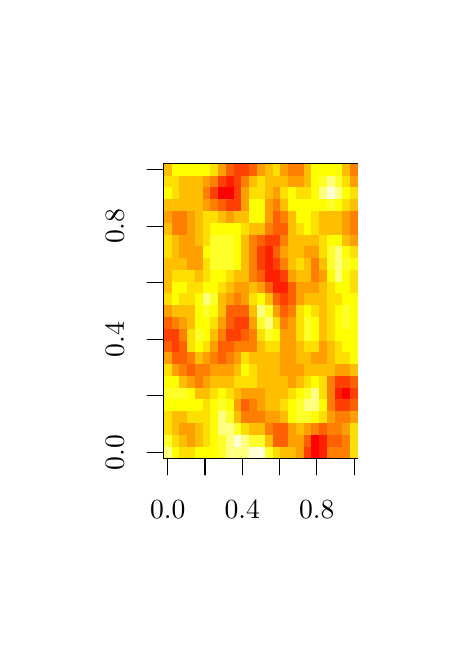
\begin{tikzpicture}[x=1pt,y=1pt]
\definecolor{fillColor}{RGB}{255,255,255}
\path[use as bounding box,fill=fillColor,fill opacity=0.00] (0,0) rectangle (144.54,216.81);
\begin{scope}
\path[clip] (  0.00,  0.00) rectangle (144.54,216.81);
\definecolor{drawColor}{RGB}{0,0,0}

\path[draw=drawColor,line width= 0.4pt,line join=round,line cap=round] ( 50.60, 61.20) -- (117.94, 61.20);

\path[draw=drawColor,line width= 0.4pt,line join=round,line cap=round] ( 50.60, 61.20) -- ( 50.60, 55.20);

\path[draw=drawColor,line width= 0.4pt,line join=round,line cap=round] ( 64.07, 61.20) -- ( 64.07, 55.20);

\path[draw=drawColor,line width= 0.4pt,line join=round,line cap=round] ( 77.54, 61.20) -- ( 77.54, 55.20);

\path[draw=drawColor,line width= 0.4pt,line join=round,line cap=round] ( 91.00, 61.20) -- ( 91.00, 55.20);

\path[draw=drawColor,line width= 0.4pt,line join=round,line cap=round] (104.47, 61.20) -- (104.47, 55.20);

\path[draw=drawColor,line width= 0.4pt,line join=round,line cap=round] (117.94, 61.20) -- (117.94, 55.20);

\node[text=drawColor,anchor=base,inner sep=0pt, outer sep=0pt, scale=  1.00] at ( 50.60, 39.60) {0.0};

\node[text=drawColor,anchor=base,inner sep=0pt, outer sep=0pt, scale=  1.00] at ( 77.54, 39.60) {0.4};

\node[text=drawColor,anchor=base,inner sep=0pt, outer sep=0pt, scale=  1.00] at (104.47, 39.60) {0.8};

\path[draw=drawColor,line width= 0.4pt,line join=round,line cap=round] ( 49.20, 63.33) -- ( 49.20,165.48);

\path[draw=drawColor,line width= 0.4pt,line join=round,line cap=round] ( 49.20, 63.33) -- ( 43.20, 63.33);

\path[draw=drawColor,line width= 0.4pt,line join=round,line cap=round] ( 49.20, 83.76) -- ( 43.20, 83.76);

\path[draw=drawColor,line width= 0.4pt,line join=round,line cap=round] ( 49.20,104.19) -- ( 43.20,104.19);

\path[draw=drawColor,line width= 0.4pt,line join=round,line cap=round] ( 49.20,124.62) -- ( 43.20,124.62);

\path[draw=drawColor,line width= 0.4pt,line join=round,line cap=round] ( 49.20,145.05) -- ( 43.20,145.05);

\path[draw=drawColor,line width= 0.4pt,line join=round,line cap=round] ( 49.20,165.48) -- ( 43.20,165.48);

\node[text=drawColor,rotate= 90.00,anchor=base,inner sep=0pt, outer sep=0pt, scale=  1.00] at ( 34.80, 63.33) {0.0};

\node[text=drawColor,rotate= 90.00,anchor=base,inner sep=0pt, outer sep=0pt, scale=  1.00] at ( 34.80,104.19) {0.4};

\node[text=drawColor,rotate= 90.00,anchor=base,inner sep=0pt, outer sep=0pt, scale=  1.00] at ( 34.80,145.05) {0.8};

\path[draw=drawColor,line width= 0.4pt,line join=round,line cap=round] ( 49.20, 61.20) --
	(119.34, 61.20) --
	(119.34,167.61) --
	( 49.20,167.61) --
	( 49.20, 61.20);
\end{scope}
\begin{scope}
\path[clip] ( 49.20, 61.20) rectangle (119.34,167.61);
\definecolor{fillColor}{RGB}{255,255,128}

\path[fill=fillColor] ( 49.20, 61.20) rectangle ( 52.01, 65.46);
\definecolor{fillColor}{RGB}{255,255,42}

\path[fill=fillColor] ( 49.20, 65.46) rectangle ( 52.01, 69.71);
\definecolor{fillColor}{RGB}{255,223,0}

\path[fill=fillColor] ( 49.20, 69.71) rectangle ( 52.01, 73.97);

\path[fill=fillColor] ( 49.20, 73.97) rectangle ( 52.01, 78.23);
\definecolor{fillColor}{RGB}{255,255,0}

\path[fill=fillColor] ( 49.20, 78.23) rectangle ( 52.01, 82.48);
\definecolor{fillColor}{RGB}{255,255,42}

\path[fill=fillColor] ( 49.20, 82.48) rectangle ( 52.01, 86.74);
\definecolor{fillColor}{RGB}{255,255,0}

\path[fill=fillColor] ( 49.20, 86.74) rectangle ( 52.01, 90.99);
\definecolor{fillColor}{RGB}{255,223,0}

\path[fill=fillColor] ( 49.20, 90.99) rectangle ( 52.01, 95.25);
\definecolor{fillColor}{RGB}{255,159,0}

\path[fill=fillColor] ( 49.20, 95.25) rectangle ( 52.01, 99.51);
\definecolor{fillColor}{RGB}{255,96,0}

\path[fill=fillColor] ( 49.20, 99.51) rectangle ( 52.01,103.76);
\definecolor{fillColor}{RGB}{255,64,0}

\path[fill=fillColor] ( 49.20,103.76) rectangle ( 52.01,108.02);
\definecolor{fillColor}{RGB}{255,96,0}

\path[fill=fillColor] ( 49.20,108.02) rectangle ( 52.01,112.28);
\definecolor{fillColor}{RGB}{255,159,0}

\path[fill=fillColor] ( 49.20,112.28) rectangle ( 52.01,116.53);
\definecolor{fillColor}{RGB}{255,223,0}

\path[fill=fillColor] ( 49.20,116.53) rectangle ( 52.01,120.79);
\definecolor{fillColor}{RGB}{255,191,0}

\path[fill=fillColor] ( 49.20,120.79) rectangle ( 52.01,125.05);

\path[fill=fillColor] ( 49.20,125.05) rectangle ( 52.01,129.30);

\path[fill=fillColor] ( 49.20,129.30) rectangle ( 52.01,133.56);
\definecolor{fillColor}{RGB}{255,223,0}

\path[fill=fillColor] ( 49.20,133.56) rectangle ( 52.01,137.82);

\path[fill=fillColor] ( 49.20,137.82) rectangle ( 52.01,142.07);
\definecolor{fillColor}{RGB}{255,191,0}

\path[fill=fillColor] ( 49.20,142.07) rectangle ( 52.01,146.33);
\definecolor{fillColor}{RGB}{255,159,0}

\path[fill=fillColor] ( 49.20,146.33) rectangle ( 52.01,150.58);
\definecolor{fillColor}{RGB}{255,191,0}

\path[fill=fillColor] ( 49.20,150.58) rectangle ( 52.01,154.84);
\definecolor{fillColor}{RGB}{255,255,0}

\path[fill=fillColor] ( 49.20,154.84) rectangle ( 52.01,159.10);
\definecolor{fillColor}{RGB}{255,223,0}

\path[fill=fillColor] ( 49.20,159.10) rectangle ( 52.01,163.35);
\definecolor{fillColor}{RGB}{255,191,0}

\path[fill=fillColor] ( 49.20,163.35) rectangle ( 52.01,167.61);
\definecolor{fillColor}{RGB}{255,255,0}

\path[fill=fillColor] ( 52.01, 61.20) rectangle ( 54.81, 65.46);
\definecolor{fillColor}{RGB}{255,223,0}

\path[fill=fillColor] ( 52.01, 65.46) rectangle ( 54.81, 69.71);
\definecolor{fillColor}{RGB}{255,191,0}

\path[fill=fillColor] ( 52.01, 69.71) rectangle ( 54.81, 73.97);

\path[fill=fillColor] ( 52.01, 73.97) rectangle ( 54.81, 78.23);
\definecolor{fillColor}{RGB}{255,255,0}

\path[fill=fillColor] ( 52.01, 78.23) rectangle ( 54.81, 82.48);
\definecolor{fillColor}{RGB}{255,255,42}

\path[fill=fillColor] ( 52.01, 82.48) rectangle ( 54.81, 86.74);
\definecolor{fillColor}{RGB}{255,255,0}

\path[fill=fillColor] ( 52.01, 86.74) rectangle ( 54.81, 90.99);
\definecolor{fillColor}{RGB}{255,159,0}

\path[fill=fillColor] ( 52.01, 90.99) rectangle ( 54.81, 95.25);
\definecolor{fillColor}{RGB}{255,96,0}

\path[fill=fillColor] ( 52.01, 95.25) rectangle ( 54.81, 99.51);
\definecolor{fillColor}{RGB}{255,64,0}

\path[fill=fillColor] ( 52.01, 99.51) rectangle ( 54.81,103.76);

\path[fill=fillColor] ( 52.01,103.76) rectangle ( 54.81,108.02);
\definecolor{fillColor}{RGB}{255,128,0}

\path[fill=fillColor] ( 52.01,108.02) rectangle ( 54.81,112.28);
\definecolor{fillColor}{RGB}{255,191,0}

\path[fill=fillColor] ( 52.01,112.28) rectangle ( 54.81,116.53);
\definecolor{fillColor}{RGB}{255,255,0}

\path[fill=fillColor] ( 52.01,116.53) rectangle ( 54.81,120.79);

\path[fill=fillColor] ( 52.01,120.79) rectangle ( 54.81,125.05);
\definecolor{fillColor}{RGB}{255,223,0}

\path[fill=fillColor] ( 52.01,125.05) rectangle ( 54.81,129.30);
\definecolor{fillColor}{RGB}{255,191,0}

\path[fill=fillColor] ( 52.01,129.30) rectangle ( 54.81,133.56);

\path[fill=fillColor] ( 52.01,133.56) rectangle ( 54.81,137.82);

\path[fill=fillColor] ( 52.01,137.82) rectangle ( 54.81,142.07);
\definecolor{fillColor}{RGB}{255,128,0}

\path[fill=fillColor] ( 52.01,142.07) rectangle ( 54.81,146.33);

\path[fill=fillColor] ( 52.01,146.33) rectangle ( 54.81,150.58);
\definecolor{fillColor}{RGB}{255,191,0}

\path[fill=fillColor] ( 52.01,150.58) rectangle ( 54.81,154.84);
\definecolor{fillColor}{RGB}{255,223,0}

\path[fill=fillColor] ( 52.01,154.84) rectangle ( 54.81,159.10);

\path[fill=fillColor] ( 52.01,159.10) rectangle ( 54.81,163.35);
\definecolor{fillColor}{RGB}{255,255,0}

\path[fill=fillColor] ( 52.01,163.35) rectangle ( 54.81,167.61);
\definecolor{fillColor}{RGB}{255,223,0}

\path[fill=fillColor] ( 54.81, 61.20) rectangle ( 57.62, 65.46);
\definecolor{fillColor}{RGB}{255,191,0}

\path[fill=fillColor] ( 54.81, 65.46) rectangle ( 57.62, 69.71);
\definecolor{fillColor}{RGB}{255,159,0}

\path[fill=fillColor] ( 54.81, 69.71) rectangle ( 57.62, 73.97);
\definecolor{fillColor}{RGB}{255,191,0}

\path[fill=fillColor] ( 54.81, 73.97) rectangle ( 57.62, 78.23);
\definecolor{fillColor}{RGB}{255,255,0}

\path[fill=fillColor] ( 54.81, 78.23) rectangle ( 57.62, 82.48);
\definecolor{fillColor}{RGB}{255,255,42}

\path[fill=fillColor] ( 54.81, 82.48) rectangle ( 57.62, 86.74);
\definecolor{fillColor}{RGB}{255,191,0}

\path[fill=fillColor] ( 54.81, 86.74) rectangle ( 57.62, 90.99);
\definecolor{fillColor}{RGB}{255,128,0}

\path[fill=fillColor] ( 54.81, 90.99) rectangle ( 57.62, 95.25);
\definecolor{fillColor}{RGB}{255,96,0}

\path[fill=fillColor] ( 54.81, 95.25) rectangle ( 57.62, 99.51);

\path[fill=fillColor] ( 54.81, 99.51) rectangle ( 57.62,103.76);
\definecolor{fillColor}{RGB}{255,128,0}

\path[fill=fillColor] ( 54.81,103.76) rectangle ( 57.62,108.02);
\definecolor{fillColor}{RGB}{255,159,0}

\path[fill=fillColor] ( 54.81,108.02) rectangle ( 57.62,112.28);
\definecolor{fillColor}{RGB}{255,191,0}

\path[fill=fillColor] ( 54.81,112.28) rectangle ( 57.62,116.53);
\definecolor{fillColor}{RGB}{255,223,0}

\path[fill=fillColor] ( 54.81,116.53) rectangle ( 57.62,120.79);
\definecolor{fillColor}{RGB}{255,255,0}

\path[fill=fillColor] ( 54.81,120.79) rectangle ( 57.62,125.05);
\definecolor{fillColor}{RGB}{255,223,0}

\path[fill=fillColor] ( 54.81,125.05) rectangle ( 57.62,129.30);
\definecolor{fillColor}{RGB}{255,191,0}

\path[fill=fillColor] ( 54.81,129.30) rectangle ( 57.62,133.56);
\definecolor{fillColor}{RGB}{255,159,0}

\path[fill=fillColor] ( 54.81,133.56) rectangle ( 57.62,137.82);

\path[fill=fillColor] ( 54.81,137.82) rectangle ( 57.62,142.07);
\definecolor{fillColor}{RGB}{255,128,0}

\path[fill=fillColor] ( 54.81,142.07) rectangle ( 57.62,146.33);

\path[fill=fillColor] ( 54.81,146.33) rectangle ( 57.62,150.58);
\definecolor{fillColor}{RGB}{255,191,0}

\path[fill=fillColor] ( 54.81,150.58) rectangle ( 57.62,154.84);

\path[fill=fillColor] ( 54.81,154.84) rectangle ( 57.62,159.10);

\path[fill=fillColor] ( 54.81,159.10) rectangle ( 57.62,163.35);
\definecolor{fillColor}{RGB}{255,255,0}

\path[fill=fillColor] ( 54.81,163.35) rectangle ( 57.62,167.61);
\definecolor{fillColor}{RGB}{255,223,0}

\path[fill=fillColor] ( 57.62, 61.20) rectangle ( 60.42, 65.46);
\definecolor{fillColor}{RGB}{255,159,0}

\path[fill=fillColor] ( 57.62, 65.46) rectangle ( 60.42, 69.71);

\path[fill=fillColor] ( 57.62, 69.71) rectangle ( 60.42, 73.97);
\definecolor{fillColor}{RGB}{255,223,0}

\path[fill=fillColor] ( 57.62, 73.97) rectangle ( 60.42, 78.23);
\definecolor{fillColor}{RGB}{255,255,0}

\path[fill=fillColor] ( 57.62, 78.23) rectangle ( 60.42, 82.48);

\path[fill=fillColor] ( 57.62, 82.48) rectangle ( 60.42, 86.74);
\definecolor{fillColor}{RGB}{255,159,0}

\path[fill=fillColor] ( 57.62, 86.74) rectangle ( 60.42, 90.99);
\definecolor{fillColor}{RGB}{255,96,0}

\path[fill=fillColor] ( 57.62, 90.99) rectangle ( 60.42, 95.25);
\definecolor{fillColor}{RGB}{255,128,0}

\path[fill=fillColor] ( 57.62, 95.25) rectangle ( 60.42, 99.51);
\definecolor{fillColor}{RGB}{255,223,0}

\path[fill=fillColor] ( 57.62, 99.51) rectangle ( 60.42,103.76);

\path[fill=fillColor] ( 57.62,103.76) rectangle ( 60.42,108.02);
\definecolor{fillColor}{RGB}{255,191,0}

\path[fill=fillColor] ( 57.62,108.02) rectangle ( 60.42,112.28);

\path[fill=fillColor] ( 57.62,112.28) rectangle ( 60.42,116.53);
\definecolor{fillColor}{RGB}{255,223,0}

\path[fill=fillColor] ( 57.62,116.53) rectangle ( 60.42,120.79);

\path[fill=fillColor] ( 57.62,120.79) rectangle ( 60.42,125.05);

\path[fill=fillColor] ( 57.62,125.05) rectangle ( 60.42,129.30);
\definecolor{fillColor}{RGB}{255,159,0}

\path[fill=fillColor] ( 57.62,129.30) rectangle ( 60.42,133.56);

\path[fill=fillColor] ( 57.62,133.56) rectangle ( 60.42,137.82);

\path[fill=fillColor] ( 57.62,137.82) rectangle ( 60.42,142.07);

\path[fill=fillColor] ( 57.62,142.07) rectangle ( 60.42,146.33);

\path[fill=fillColor] ( 57.62,146.33) rectangle ( 60.42,150.58);
\definecolor{fillColor}{RGB}{255,191,0}

\path[fill=fillColor] ( 57.62,150.58) rectangle ( 60.42,154.84);

\path[fill=fillColor] ( 57.62,154.84) rectangle ( 60.42,159.10);

\path[fill=fillColor] ( 57.62,159.10) rectangle ( 60.42,163.35);
\definecolor{fillColor}{RGB}{255,255,0}

\path[fill=fillColor] ( 57.62,163.35) rectangle ( 60.42,167.61);

\path[fill=fillColor] ( 60.42, 61.20) rectangle ( 63.23, 65.46);
\definecolor{fillColor}{RGB}{255,191,0}

\path[fill=fillColor] ( 60.42, 65.46) rectangle ( 63.23, 69.71);

\path[fill=fillColor] ( 60.42, 69.71) rectangle ( 63.23, 73.97);
\definecolor{fillColor}{RGB}{255,223,0}

\path[fill=fillColor] ( 60.42, 73.97) rectangle ( 63.23, 78.23);
\definecolor{fillColor}{RGB}{255,255,0}

\path[fill=fillColor] ( 60.42, 78.23) rectangle ( 63.23, 82.48);
\definecolor{fillColor}{RGB}{255,191,0}

\path[fill=fillColor] ( 60.42, 82.48) rectangle ( 63.23, 86.74);
\definecolor{fillColor}{RGB}{255,128,0}

\path[fill=fillColor] ( 60.42, 86.74) rectangle ( 63.23, 90.99);

\path[fill=fillColor] ( 60.42, 90.99) rectangle ( 63.23, 95.25);
\definecolor{fillColor}{RGB}{255,191,0}

\path[fill=fillColor] ( 60.42, 95.25) rectangle ( 63.23, 99.51);
\definecolor{fillColor}{RGB}{255,255,0}

\path[fill=fillColor] ( 60.42, 99.51) rectangle ( 63.23,103.76);
\definecolor{fillColor}{RGB}{255,255,42}

\path[fill=fillColor] ( 60.42,103.76) rectangle ( 63.23,108.02);
\definecolor{fillColor}{RGB}{255,255,0}

\path[fill=fillColor] ( 60.42,108.02) rectangle ( 63.23,112.28);

\path[fill=fillColor] ( 60.42,112.28) rectangle ( 63.23,116.53);

\path[fill=fillColor] ( 60.42,116.53) rectangle ( 63.23,120.79);
\definecolor{fillColor}{RGB}{255,223,0}

\path[fill=fillColor] ( 60.42,120.79) rectangle ( 63.23,125.05);
\definecolor{fillColor}{RGB}{255,191,0}

\path[fill=fillColor] ( 60.42,125.05) rectangle ( 63.23,129.30);
\definecolor{fillColor}{RGB}{255,159,0}

\path[fill=fillColor] ( 60.42,129.30) rectangle ( 63.23,133.56);

\path[fill=fillColor] ( 60.42,133.56) rectangle ( 63.23,137.82);
\definecolor{fillColor}{RGB}{255,191,0}

\path[fill=fillColor] ( 60.42,137.82) rectangle ( 63.23,142.07);

\path[fill=fillColor] ( 60.42,142.07) rectangle ( 63.23,146.33);

\path[fill=fillColor] ( 60.42,146.33) rectangle ( 63.23,150.58);

\path[fill=fillColor] ( 60.42,150.58) rectangle ( 63.23,154.84);

\path[fill=fillColor] ( 60.42,154.84) rectangle ( 63.23,159.10);

\path[fill=fillColor] ( 60.42,159.10) rectangle ( 63.23,163.35);
\definecolor{fillColor}{RGB}{255,255,0}

\path[fill=fillColor] ( 60.42,163.35) rectangle ( 63.23,167.61);

\path[fill=fillColor] ( 63.23, 61.20) rectangle ( 66.03, 65.46);
\definecolor{fillColor}{RGB}{255,223,0}

\path[fill=fillColor] ( 63.23, 65.46) rectangle ( 66.03, 69.71);

\path[fill=fillColor] ( 63.23, 69.71) rectangle ( 66.03, 73.97);

\path[fill=fillColor] ( 63.23, 73.97) rectangle ( 66.03, 78.23);

\path[fill=fillColor] ( 63.23, 78.23) rectangle ( 66.03, 82.48);
\definecolor{fillColor}{RGB}{255,191,0}

\path[fill=fillColor] ( 63.23, 82.48) rectangle ( 66.03, 86.74);
\definecolor{fillColor}{RGB}{255,159,0}

\path[fill=fillColor] ( 63.23, 86.74) rectangle ( 66.03, 90.99);
\definecolor{fillColor}{RGB}{255,128,0}

\path[fill=fillColor] ( 63.23, 90.99) rectangle ( 66.03, 95.25);
\definecolor{fillColor}{RGB}{255,159,0}

\path[fill=fillColor] ( 63.23, 95.25) rectangle ( 66.03, 99.51);
\definecolor{fillColor}{RGB}{255,223,0}

\path[fill=fillColor] ( 63.23, 99.51) rectangle ( 66.03,103.76);
\definecolor{fillColor}{RGB}{255,255,0}

\path[fill=fillColor] ( 63.23,103.76) rectangle ( 66.03,108.02);

\path[fill=fillColor] ( 63.23,108.02) rectangle ( 66.03,112.28);
\definecolor{fillColor}{RGB}{255,255,42}

\path[fill=fillColor] ( 63.23,112.28) rectangle ( 66.03,116.53);
\definecolor{fillColor}{RGB}{255,255,128}

\path[fill=fillColor] ( 63.23,116.53) rectangle ( 66.03,120.79);
\definecolor{fillColor}{RGB}{255,255,0}

\path[fill=fillColor] ( 63.23,120.79) rectangle ( 66.03,125.05);
\definecolor{fillColor}{RGB}{255,223,0}

\path[fill=fillColor] ( 63.23,125.05) rectangle ( 66.03,129.30);

\path[fill=fillColor] ( 63.23,129.30) rectangle ( 66.03,133.56);
\definecolor{fillColor}{RGB}{255,255,0}

\path[fill=fillColor] ( 63.23,133.56) rectangle ( 66.03,137.82);
\definecolor{fillColor}{RGB}{255,223,0}

\path[fill=fillColor] ( 63.23,137.82) rectangle ( 66.03,142.07);

\path[fill=fillColor] ( 63.23,142.07) rectangle ( 66.03,146.33);

\path[fill=fillColor] ( 63.23,146.33) rectangle ( 66.03,150.58);
\definecolor{fillColor}{RGB}{255,159,0}

\path[fill=fillColor] ( 63.23,150.58) rectangle ( 66.03,154.84);
\definecolor{fillColor}{RGB}{255,128,0}

\path[fill=fillColor] ( 63.23,154.84) rectangle ( 66.03,159.10);
\definecolor{fillColor}{RGB}{255,159,0}

\path[fill=fillColor] ( 63.23,159.10) rectangle ( 66.03,163.35);
\definecolor{fillColor}{RGB}{255,255,0}

\path[fill=fillColor] ( 63.23,163.35) rectangle ( 66.03,167.61);

\path[fill=fillColor] ( 66.03, 61.20) rectangle ( 68.84, 65.46);

\path[fill=fillColor] ( 66.03, 65.46) rectangle ( 68.84, 69.71);

\path[fill=fillColor] ( 66.03, 69.71) rectangle ( 68.84, 73.97);

\path[fill=fillColor] ( 66.03, 73.97) rectangle ( 68.84, 78.23);

\path[fill=fillColor] ( 66.03, 78.23) rectangle ( 68.84, 82.48);
\definecolor{fillColor}{RGB}{255,223,0}

\path[fill=fillColor] ( 66.03, 82.48) rectangle ( 68.84, 86.74);
\definecolor{fillColor}{RGB}{255,191,0}

\path[fill=fillColor] ( 66.03, 86.74) rectangle ( 68.84, 90.99);
\definecolor{fillColor}{RGB}{255,159,0}

\path[fill=fillColor] ( 66.03, 90.99) rectangle ( 68.84, 95.25);
\definecolor{fillColor}{RGB}{255,128,0}

\path[fill=fillColor] ( 66.03, 95.25) rectangle ( 68.84, 99.51);
\definecolor{fillColor}{RGB}{255,159,0}

\path[fill=fillColor] ( 66.03, 99.51) rectangle ( 68.84,103.76);
\definecolor{fillColor}{RGB}{255,191,0}

\path[fill=fillColor] ( 66.03,103.76) rectangle ( 68.84,108.02);
\definecolor{fillColor}{RGB}{255,223,0}

\path[fill=fillColor] ( 66.03,108.02) rectangle ( 68.84,112.28);
\definecolor{fillColor}{RGB}{255,255,0}

\path[fill=fillColor] ( 66.03,112.28) rectangle ( 68.84,116.53);
\definecolor{fillColor}{RGB}{255,255,42}

\path[fill=fillColor] ( 66.03,116.53) rectangle ( 68.84,120.79);
\definecolor{fillColor}{RGB}{255,255,0}

\path[fill=fillColor] ( 66.03,120.79) rectangle ( 68.84,125.05);

\path[fill=fillColor] ( 66.03,125.05) rectangle ( 68.84,129.30);
\definecolor{fillColor}{RGB}{255,255,42}

\path[fill=fillColor] ( 66.03,129.30) rectangle ( 68.84,133.56);

\path[fill=fillColor] ( 66.03,133.56) rectangle ( 68.84,137.82);

\path[fill=fillColor] ( 66.03,137.82) rectangle ( 68.84,142.07);
\definecolor{fillColor}{RGB}{255,255,0}

\path[fill=fillColor] ( 66.03,142.07) rectangle ( 68.84,146.33);
\definecolor{fillColor}{RGB}{255,223,0}

\path[fill=fillColor] ( 66.03,146.33) rectangle ( 68.84,150.58);
\definecolor{fillColor}{RGB}{255,128,0}

\path[fill=fillColor] ( 66.03,150.58) rectangle ( 68.84,154.84);
\definecolor{fillColor}{RGB}{255,64,0}

\path[fill=fillColor] ( 66.03,154.84) rectangle ( 68.84,159.10);
\definecolor{fillColor}{RGB}{255,128,0}

\path[fill=fillColor] ( 66.03,159.10) rectangle ( 68.84,163.35);
\definecolor{fillColor}{RGB}{255,223,0}

\path[fill=fillColor] ( 66.03,163.35) rectangle ( 68.84,167.61);
\definecolor{fillColor}{RGB}{255,255,42}

\path[fill=fillColor] ( 68.84, 61.20) rectangle ( 71.64, 65.46);

\path[fill=fillColor] ( 68.84, 65.46) rectangle ( 71.64, 69.71);
\definecolor{fillColor}{RGB}{255,255,128}

\path[fill=fillColor] ( 68.84, 69.71) rectangle ( 71.64, 73.97);

\path[fill=fillColor] ( 68.84, 73.97) rectangle ( 71.64, 78.23);
\definecolor{fillColor}{RGB}{255,255,42}

\path[fill=fillColor] ( 68.84, 78.23) rectangle ( 71.64, 82.48);
\definecolor{fillColor}{RGB}{255,255,0}

\path[fill=fillColor] ( 68.84, 82.48) rectangle ( 71.64, 86.74);
\definecolor{fillColor}{RGB}{255,191,0}

\path[fill=fillColor] ( 68.84, 86.74) rectangle ( 71.64, 90.99);
\definecolor{fillColor}{RGB}{255,159,0}

\path[fill=fillColor] ( 68.84, 90.99) rectangle ( 71.64, 95.25);
\definecolor{fillColor}{RGB}{255,96,0}

\path[fill=fillColor] ( 68.84, 95.25) rectangle ( 71.64, 99.51);

\path[fill=fillColor] ( 68.84, 99.51) rectangle ( 71.64,103.76);
\definecolor{fillColor}{RGB}{255,128,0}

\path[fill=fillColor] ( 68.84,103.76) rectangle ( 71.64,108.02);
\definecolor{fillColor}{RGB}{255,159,0}

\path[fill=fillColor] ( 68.84,108.02) rectangle ( 71.64,112.28);
\definecolor{fillColor}{RGB}{255,191,0}

\path[fill=fillColor] ( 68.84,112.28) rectangle ( 71.64,116.53);

\path[fill=fillColor] ( 68.84,116.53) rectangle ( 71.64,120.79);
\definecolor{fillColor}{RGB}{255,223,0}

\path[fill=fillColor] ( 68.84,120.79) rectangle ( 71.64,125.05);
\definecolor{fillColor}{RGB}{255,255,0}

\path[fill=fillColor] ( 68.84,125.05) rectangle ( 71.64,129.30);
\definecolor{fillColor}{RGB}{255,255,42}

\path[fill=fillColor] ( 68.84,129.30) rectangle ( 71.64,133.56);

\path[fill=fillColor] ( 68.84,133.56) rectangle ( 71.64,137.82);

\path[fill=fillColor] ( 68.84,137.82) rectangle ( 71.64,142.07);
\definecolor{fillColor}{RGB}{255,255,0}

\path[fill=fillColor] ( 68.84,142.07) rectangle ( 71.64,146.33);
\definecolor{fillColor}{RGB}{255,191,0}

\path[fill=fillColor] ( 68.84,146.33) rectangle ( 71.64,150.58);
\definecolor{fillColor}{RGB}{255,96,0}

\path[fill=fillColor] ( 68.84,150.58) rectangle ( 71.64,154.84);
\definecolor{fillColor}{RGB}{255,0,0}

\path[fill=fillColor] ( 68.84,154.84) rectangle ( 71.64,159.10);
\definecolor{fillColor}{RGB}{255,64,0}

\path[fill=fillColor] ( 68.84,159.10) rectangle ( 71.64,163.35);
\definecolor{fillColor}{RGB}{255,159,0}

\path[fill=fillColor] ( 68.84,163.35) rectangle ( 71.64,167.61);
\definecolor{fillColor}{RGB}{255,255,128}

\path[fill=fillColor] ( 71.64, 61.20) rectangle ( 74.45, 65.46);

\path[fill=fillColor] ( 71.64, 65.46) rectangle ( 74.45, 69.71);

\path[fill=fillColor] ( 71.64, 69.71) rectangle ( 74.45, 73.97);
\definecolor{fillColor}{RGB}{255,255,42}

\path[fill=fillColor] ( 71.64, 73.97) rectangle ( 74.45, 78.23);
\definecolor{fillColor}{RGB}{255,255,0}

\path[fill=fillColor] ( 71.64, 78.23) rectangle ( 74.45, 82.48);
\definecolor{fillColor}{RGB}{255,223,0}

\path[fill=fillColor] ( 71.64, 82.48) rectangle ( 74.45, 86.74);
\definecolor{fillColor}{RGB}{255,191,0}

\path[fill=fillColor] ( 71.64, 86.74) rectangle ( 74.45, 90.99);
\definecolor{fillColor}{RGB}{255,159,0}

\path[fill=fillColor] ( 71.64, 90.99) rectangle ( 74.45, 95.25);
\definecolor{fillColor}{RGB}{255,128,0}

\path[fill=fillColor] ( 71.64, 95.25) rectangle ( 74.45, 99.51);
\definecolor{fillColor}{RGB}{255,96,0}

\path[fill=fillColor] ( 71.64, 99.51) rectangle ( 74.45,103.76);
\definecolor{fillColor}{RGB}{255,64,0}

\path[fill=fillColor] ( 71.64,103.76) rectangle ( 74.45,108.02);
\definecolor{fillColor}{RGB}{255,96,0}

\path[fill=fillColor] ( 71.64,108.02) rectangle ( 74.45,112.28);

\path[fill=fillColor] ( 71.64,112.28) rectangle ( 74.45,116.53);
\definecolor{fillColor}{RGB}{255,159,0}

\path[fill=fillColor] ( 71.64,116.53) rectangle ( 74.45,120.79);
\definecolor{fillColor}{RGB}{255,191,0}

\path[fill=fillColor] ( 71.64,120.79) rectangle ( 74.45,125.05);
\definecolor{fillColor}{RGB}{255,223,0}

\path[fill=fillColor] ( 71.64,125.05) rectangle ( 74.45,129.30);
\definecolor{fillColor}{RGB}{255,255,42}

\path[fill=fillColor] ( 71.64,129.30) rectangle ( 74.45,133.56);

\path[fill=fillColor] ( 71.64,133.56) rectangle ( 74.45,137.82);

\path[fill=fillColor] ( 71.64,137.82) rectangle ( 74.45,142.07);
\definecolor{fillColor}{RGB}{255,255,0}

\path[fill=fillColor] ( 71.64,142.07) rectangle ( 74.45,146.33);
\definecolor{fillColor}{RGB}{255,159,0}

\path[fill=fillColor] ( 71.64,146.33) rectangle ( 74.45,150.58);
\definecolor{fillColor}{RGB}{255,64,0}

\path[fill=fillColor] ( 71.64,150.58) rectangle ( 74.45,154.84);
\definecolor{fillColor}{RGB}{255,0,0}

\path[fill=fillColor] ( 71.64,154.84) rectangle ( 74.45,159.10);
\definecolor{fillColor}{RGB}{255,32,0}

\path[fill=fillColor] ( 71.64,159.10) rectangle ( 74.45,163.35);
\definecolor{fillColor}{RGB}{255,96,0}

\path[fill=fillColor] ( 71.64,163.35) rectangle ( 74.45,167.61);
\definecolor{fillColor}{RGB}{255,255,128}

\path[fill=fillColor] ( 74.45, 61.20) rectangle ( 77.26, 65.46);
\definecolor{fillColor}{RGB}{255,255,213}

\path[fill=fillColor] ( 74.45, 65.46) rectangle ( 77.26, 69.71);
\definecolor{fillColor}{RGB}{255,255,42}

\path[fill=fillColor] ( 74.45, 69.71) rectangle ( 77.26, 73.97);
\definecolor{fillColor}{RGB}{255,191,0}

\path[fill=fillColor] ( 74.45, 73.97) rectangle ( 77.26, 78.23);
\definecolor{fillColor}{RGB}{255,159,0}

\path[fill=fillColor] ( 74.45, 78.23) rectangle ( 77.26, 82.48);
\definecolor{fillColor}{RGB}{255,191,0}

\path[fill=fillColor] ( 74.45, 82.48) rectangle ( 77.26, 86.74);
\definecolor{fillColor}{RGB}{255,223,0}

\path[fill=fillColor] ( 74.45, 86.74) rectangle ( 77.26, 90.99);
\definecolor{fillColor}{RGB}{255,191,0}

\path[fill=fillColor] ( 74.45, 90.99) rectangle ( 77.26, 95.25);
\definecolor{fillColor}{RGB}{255,159,0}

\path[fill=fillColor] ( 74.45, 95.25) rectangle ( 77.26, 99.51);
\definecolor{fillColor}{RGB}{255,128,0}

\path[fill=fillColor] ( 74.45, 99.51) rectangle ( 77.26,103.76);
\definecolor{fillColor}{RGB}{255,64,0}

\path[fill=fillColor] ( 74.45,103.76) rectangle ( 77.26,108.02);

\path[fill=fillColor] ( 74.45,108.02) rectangle ( 77.26,112.28);
\definecolor{fillColor}{RGB}{255,96,0}

\path[fill=fillColor] ( 74.45,112.28) rectangle ( 77.26,116.53);
\definecolor{fillColor}{RGB}{255,128,0}

\path[fill=fillColor] ( 74.45,116.53) rectangle ( 77.26,120.79);
\definecolor{fillColor}{RGB}{255,159,0}

\path[fill=fillColor] ( 74.45,120.79) rectangle ( 77.26,125.05);
\definecolor{fillColor}{RGB}{255,191,0}

\path[fill=fillColor] ( 74.45,125.05) rectangle ( 77.26,129.30);
\definecolor{fillColor}{RGB}{255,255,0}

\path[fill=fillColor] ( 74.45,129.30) rectangle ( 77.26,133.56);

\path[fill=fillColor] ( 74.45,133.56) rectangle ( 77.26,137.82);

\path[fill=fillColor] ( 74.45,137.82) rectangle ( 77.26,142.07);

\path[fill=fillColor] ( 74.45,142.07) rectangle ( 77.26,146.33);
\definecolor{fillColor}{RGB}{255,191,0}

\path[fill=fillColor] ( 74.45,146.33) rectangle ( 77.26,150.58);
\definecolor{fillColor}{RGB}{255,64,0}

\path[fill=fillColor] ( 74.45,150.58) rectangle ( 77.26,154.84);

\path[fill=fillColor] ( 74.45,154.84) rectangle ( 77.26,159.10);

\path[fill=fillColor] ( 74.45,159.10) rectangle ( 77.26,163.35);

\path[fill=fillColor] ( 74.45,163.35) rectangle ( 77.26,167.61);
\definecolor{fillColor}{RGB}{255,255,128}

\path[fill=fillColor] ( 77.26, 61.20) rectangle ( 80.06, 65.46);

\path[fill=fillColor] ( 77.26, 65.46) rectangle ( 80.06, 69.71);
\definecolor{fillColor}{RGB}{255,223,0}

\path[fill=fillColor] ( 77.26, 69.71) rectangle ( 80.06, 73.97);
\definecolor{fillColor}{RGB}{255,128,0}

\path[fill=fillColor] ( 77.26, 73.97) rectangle ( 80.06, 78.23);
\definecolor{fillColor}{RGB}{255,96,0}

\path[fill=fillColor] ( 77.26, 78.23) rectangle ( 80.06, 82.48);
\definecolor{fillColor}{RGB}{255,159,0}

\path[fill=fillColor] ( 77.26, 82.48) rectangle ( 80.06, 86.74);
\definecolor{fillColor}{RGB}{255,223,0}

\path[fill=fillColor] ( 77.26, 86.74) rectangle ( 80.06, 90.99);
\definecolor{fillColor}{RGB}{255,255,0}

\path[fill=fillColor] ( 77.26, 90.99) rectangle ( 80.06, 95.25);
\definecolor{fillColor}{RGB}{255,223,0}

\path[fill=fillColor] ( 77.26, 95.25) rectangle ( 80.06, 99.51);
\definecolor{fillColor}{RGB}{255,128,0}

\path[fill=fillColor] ( 77.26, 99.51) rectangle ( 80.06,103.76);
\definecolor{fillColor}{RGB}{255,96,0}

\path[fill=fillColor] ( 77.26,103.76) rectangle ( 80.06,108.02);
\definecolor{fillColor}{RGB}{255,64,0}

\path[fill=fillColor] ( 77.26,108.02) rectangle ( 80.06,112.28);
\definecolor{fillColor}{RGB}{255,96,0}

\path[fill=fillColor] ( 77.26,112.28) rectangle ( 80.06,116.53);
\definecolor{fillColor}{RGB}{255,159,0}

\path[fill=fillColor] ( 77.26,116.53) rectangle ( 80.06,120.79);

\path[fill=fillColor] ( 77.26,120.79) rectangle ( 80.06,125.05);
\definecolor{fillColor}{RGB}{255,191,0}

\path[fill=fillColor] ( 77.26,125.05) rectangle ( 80.06,129.30);

\path[fill=fillColor] ( 77.26,129.30) rectangle ( 80.06,133.56);

\path[fill=fillColor] ( 77.26,133.56) rectangle ( 80.06,137.82);

\path[fill=fillColor] ( 77.26,137.82) rectangle ( 80.06,142.07);
\definecolor{fillColor}{RGB}{255,223,0}

\path[fill=fillColor] ( 77.26,142.07) rectangle ( 80.06,146.33);
\definecolor{fillColor}{RGB}{255,191,0}

\path[fill=fillColor] ( 77.26,146.33) rectangle ( 80.06,150.58);
\definecolor{fillColor}{RGB}{255,159,0}

\path[fill=fillColor] ( 77.26,150.58) rectangle ( 80.06,154.84);

\path[fill=fillColor] ( 77.26,154.84) rectangle ( 80.06,159.10);
\definecolor{fillColor}{RGB}{255,128,0}

\path[fill=fillColor] ( 77.26,159.10) rectangle ( 80.06,163.35);
\definecolor{fillColor}{RGB}{255,64,0}

\path[fill=fillColor] ( 77.26,163.35) rectangle ( 80.06,167.61);
\definecolor{fillColor}{RGB}{255,255,213}

\path[fill=fillColor] ( 80.06, 61.20) rectangle ( 82.87, 65.46);
\definecolor{fillColor}{RGB}{255,255,42}

\path[fill=fillColor] ( 80.06, 65.46) rectangle ( 82.87, 69.71);
\definecolor{fillColor}{RGB}{255,191,0}

\path[fill=fillColor] ( 80.06, 69.71) rectangle ( 82.87, 73.97);
\definecolor{fillColor}{RGB}{255,128,0}

\path[fill=fillColor] ( 80.06, 73.97) rectangle ( 82.87, 78.23);

\path[fill=fillColor] ( 80.06, 78.23) rectangle ( 82.87, 82.48);
\definecolor{fillColor}{RGB}{255,159,0}

\path[fill=fillColor] ( 80.06, 82.48) rectangle ( 82.87, 86.74);
\definecolor{fillColor}{RGB}{255,223,0}

\path[fill=fillColor] ( 80.06, 86.74) rectangle ( 82.87, 90.99);

\path[fill=fillColor] ( 80.06, 90.99) rectangle ( 82.87, 95.25);
\definecolor{fillColor}{RGB}{255,191,0}

\path[fill=fillColor] ( 80.06, 95.25) rectangle ( 82.87, 99.51);
\definecolor{fillColor}{RGB}{255,128,0}

\path[fill=fillColor] ( 80.06, 99.51) rectangle ( 82.87,103.76);

\path[fill=fillColor] ( 80.06,103.76) rectangle ( 82.87,108.02);
\definecolor{fillColor}{RGB}{255,159,0}

\path[fill=fillColor] ( 80.06,108.02) rectangle ( 82.87,112.28);
\definecolor{fillColor}{RGB}{255,191,0}

\path[fill=fillColor] ( 80.06,112.28) rectangle ( 82.87,116.53);
\definecolor{fillColor}{RGB}{255,223,0}

\path[fill=fillColor] ( 80.06,116.53) rectangle ( 82.87,120.79);
\definecolor{fillColor}{RGB}{255,191,0}

\path[fill=fillColor] ( 80.06,120.79) rectangle ( 82.87,125.05);
\definecolor{fillColor}{RGB}{255,128,0}

\path[fill=fillColor] ( 80.06,125.05) rectangle ( 82.87,129.30);

\path[fill=fillColor] ( 80.06,129.30) rectangle ( 82.87,133.56);

\path[fill=fillColor] ( 80.06,133.56) rectangle ( 82.87,137.82);

\path[fill=fillColor] ( 80.06,137.82) rectangle ( 82.87,142.07);
\definecolor{fillColor}{RGB}{255,191,0}

\path[fill=fillColor] ( 80.06,142.07) rectangle ( 82.87,146.33);
\definecolor{fillColor}{RGB}{255,255,0}

\path[fill=fillColor] ( 80.06,146.33) rectangle ( 82.87,150.58);

\path[fill=fillColor] ( 80.06,150.58) rectangle ( 82.87,154.84);
\definecolor{fillColor}{RGB}{255,223,0}

\path[fill=fillColor] ( 80.06,154.84) rectangle ( 82.87,159.10);
\definecolor{fillColor}{RGB}{255,191,0}

\path[fill=fillColor] ( 80.06,159.10) rectangle ( 82.87,163.35);
\definecolor{fillColor}{RGB}{255,96,0}

\path[fill=fillColor] ( 80.06,163.35) rectangle ( 82.87,167.61);
\definecolor{fillColor}{RGB}{255,255,213}

\path[fill=fillColor] ( 82.87, 61.20) rectangle ( 85.67, 65.46);
\definecolor{fillColor}{RGB}{255,255,42}

\path[fill=fillColor] ( 82.87, 65.46) rectangle ( 85.67, 69.71);
\definecolor{fillColor}{RGB}{255,191,0}

\path[fill=fillColor] ( 82.87, 69.71) rectangle ( 85.67, 73.97);
\definecolor{fillColor}{RGB}{255,128,0}

\path[fill=fillColor] ( 82.87, 73.97) rectangle ( 85.67, 78.23);
\definecolor{fillColor}{RGB}{255,159,0}

\path[fill=fillColor] ( 82.87, 78.23) rectangle ( 85.67, 82.48);

\path[fill=fillColor] ( 82.87, 82.48) rectangle ( 85.67, 86.74);
\definecolor{fillColor}{RGB}{255,191,0}

\path[fill=fillColor] ( 82.87, 86.74) rectangle ( 85.67, 90.99);

\path[fill=fillColor] ( 82.87, 90.99) rectangle ( 85.67, 95.25);

\path[fill=fillColor] ( 82.87, 95.25) rectangle ( 85.67, 99.51);

\path[fill=fillColor] ( 82.87, 99.51) rectangle ( 85.67,103.76);
\definecolor{fillColor}{RGB}{255,223,0}

\path[fill=fillColor] ( 82.87,103.76) rectangle ( 85.67,108.02);
\definecolor{fillColor}{RGB}{255,255,42}

\path[fill=fillColor] ( 82.87,108.02) rectangle ( 85.67,112.28);
\definecolor{fillColor}{RGB}{255,255,128}

\path[fill=fillColor] ( 82.87,112.28) rectangle ( 85.67,116.53);
\definecolor{fillColor}{RGB}{255,255,0}

\path[fill=fillColor] ( 82.87,116.53) rectangle ( 85.67,120.79);
\definecolor{fillColor}{RGB}{255,159,0}

\path[fill=fillColor] ( 82.87,120.79) rectangle ( 85.67,125.05);
\definecolor{fillColor}{RGB}{255,96,0}

\path[fill=fillColor] ( 82.87,125.05) rectangle ( 85.67,129.30);
\definecolor{fillColor}{RGB}{255,64,0}

\path[fill=fillColor] ( 82.87,129.30) rectangle ( 85.67,133.56);

\path[fill=fillColor] ( 82.87,133.56) rectangle ( 85.67,137.82);
\definecolor{fillColor}{RGB}{255,96,0}

\path[fill=fillColor] ( 82.87,137.82) rectangle ( 85.67,142.07);
\definecolor{fillColor}{RGB}{255,191,0}

\path[fill=fillColor] ( 82.87,142.07) rectangle ( 85.67,146.33);
\definecolor{fillColor}{RGB}{255,255,0}

\path[fill=fillColor] ( 82.87,146.33) rectangle ( 85.67,150.58);

\path[fill=fillColor] ( 82.87,150.58) rectangle ( 85.67,154.84);
\definecolor{fillColor}{RGB}{255,223,0}

\path[fill=fillColor] ( 82.87,154.84) rectangle ( 85.67,159.10);

\path[fill=fillColor] ( 82.87,159.10) rectangle ( 85.67,163.35);
\definecolor{fillColor}{RGB}{255,159,0}

\path[fill=fillColor] ( 82.87,163.35) rectangle ( 85.67,167.61);
\definecolor{fillColor}{RGB}{255,255,42}

\path[fill=fillColor] ( 85.67, 61.20) rectangle ( 88.48, 65.46);
\definecolor{fillColor}{RGB}{255,191,0}

\path[fill=fillColor] ( 85.67, 65.46) rectangle ( 88.48, 69.71);
\definecolor{fillColor}{RGB}{255,128,0}

\path[fill=fillColor] ( 85.67, 69.71) rectangle ( 88.48, 73.97);
\definecolor{fillColor}{RGB}{255,159,0}

\path[fill=fillColor] ( 85.67, 73.97) rectangle ( 88.48, 78.23);
\definecolor{fillColor}{RGB}{255,191,0}

\path[fill=fillColor] ( 85.67, 78.23) rectangle ( 88.48, 82.48);

\path[fill=fillColor] ( 85.67, 82.48) rectangle ( 88.48, 86.74);

\path[fill=fillColor] ( 85.67, 86.74) rectangle ( 88.48, 90.99);

\path[fill=fillColor] ( 85.67, 90.99) rectangle ( 88.48, 95.25);

\path[fill=fillColor] ( 85.67, 95.25) rectangle ( 88.48, 99.51);
\definecolor{fillColor}{RGB}{255,223,0}

\path[fill=fillColor] ( 85.67, 99.51) rectangle ( 88.48,103.76);
\definecolor{fillColor}{RGB}{255,255,42}

\path[fill=fillColor] ( 85.67,103.76) rectangle ( 88.48,108.02);
\definecolor{fillColor}{RGB}{255,255,128}

\path[fill=fillColor] ( 85.67,108.02) rectangle ( 88.48,112.28);
\definecolor{fillColor}{RGB}{255,255,42}

\path[fill=fillColor] ( 85.67,112.28) rectangle ( 88.48,116.53);
\definecolor{fillColor}{RGB}{255,191,0}

\path[fill=fillColor] ( 85.67,116.53) rectangle ( 88.48,120.79);
\definecolor{fillColor}{RGB}{255,96,0}

\path[fill=fillColor] ( 85.67,120.79) rectangle ( 88.48,125.05);
\definecolor{fillColor}{RGB}{255,32,0}

\path[fill=fillColor] ( 85.67,125.05) rectangle ( 88.48,129.30);

\path[fill=fillColor] ( 85.67,129.30) rectangle ( 88.48,133.56);

\path[fill=fillColor] ( 85.67,133.56) rectangle ( 88.48,137.82);
\definecolor{fillColor}{RGB}{255,64,0}

\path[fill=fillColor] ( 85.67,137.82) rectangle ( 88.48,142.07);
\definecolor{fillColor}{RGB}{255,128,0}

\path[fill=fillColor] ( 85.67,142.07) rectangle ( 88.48,146.33);
\definecolor{fillColor}{RGB}{255,159,0}

\path[fill=fillColor] ( 85.67,146.33) rectangle ( 88.48,150.58);

\path[fill=fillColor] ( 85.67,150.58) rectangle ( 88.48,154.84);
\definecolor{fillColor}{RGB}{255,191,0}

\path[fill=fillColor] ( 85.67,154.84) rectangle ( 88.48,159.10);

\path[fill=fillColor] ( 85.67,159.10) rectangle ( 88.48,163.35);

\path[fill=fillColor] ( 85.67,163.35) rectangle ( 88.48,167.61);
\definecolor{fillColor}{RGB}{255,223,0}

\path[fill=fillColor] ( 88.48, 61.20) rectangle ( 91.28, 65.46);
\definecolor{fillColor}{RGB}{255,96,0}

\path[fill=fillColor] ( 88.48, 65.46) rectangle ( 91.28, 69.71);

\path[fill=fillColor] ( 88.48, 69.71) rectangle ( 91.28, 73.97);
\definecolor{fillColor}{RGB}{255,159,0}

\path[fill=fillColor] ( 88.48, 73.97) rectangle ( 91.28, 78.23);
\definecolor{fillColor}{RGB}{255,191,0}

\path[fill=fillColor] ( 88.48, 78.23) rectangle ( 91.28, 82.48);

\path[fill=fillColor] ( 88.48, 82.48) rectangle ( 91.28, 86.74);

\path[fill=fillColor] ( 88.48, 86.74) rectangle ( 91.28, 90.99);

\path[fill=fillColor] ( 88.48, 90.99) rectangle ( 91.28, 95.25);

\path[fill=fillColor] ( 88.48, 95.25) rectangle ( 91.28, 99.51);
\definecolor{fillColor}{RGB}{255,223,0}

\path[fill=fillColor] ( 88.48, 99.51) rectangle ( 91.28,103.76);
\definecolor{fillColor}{RGB}{255,255,0}

\path[fill=fillColor] ( 88.48,103.76) rectangle ( 91.28,108.02);
\definecolor{fillColor}{RGB}{255,223,0}

\path[fill=fillColor] ( 88.48,108.02) rectangle ( 91.28,112.28);
\definecolor{fillColor}{RGB}{255,159,0}

\path[fill=fillColor] ( 88.48,112.28) rectangle ( 91.28,116.53);
\definecolor{fillColor}{RGB}{255,96,0}

\path[fill=fillColor] ( 88.48,116.53) rectangle ( 91.28,120.79);
\definecolor{fillColor}{RGB}{255,32,0}

\path[fill=fillColor] ( 88.48,120.79) rectangle ( 91.28,125.05);

\path[fill=fillColor] ( 88.48,125.05) rectangle ( 91.28,129.30);
\definecolor{fillColor}{RGB}{255,64,0}

\path[fill=fillColor] ( 88.48,129.30) rectangle ( 91.28,133.56);
\definecolor{fillColor}{RGB}{255,96,0}

\path[fill=fillColor] ( 88.48,133.56) rectangle ( 91.28,137.82);
\definecolor{fillColor}{RGB}{255,64,0}

\path[fill=fillColor] ( 88.48,137.82) rectangle ( 91.28,142.07);
\definecolor{fillColor}{RGB}{255,96,0}

\path[fill=fillColor] ( 88.48,142.07) rectangle ( 91.28,146.33);

\path[fill=fillColor] ( 88.48,146.33) rectangle ( 91.28,150.58);
\definecolor{fillColor}{RGB}{255,128,0}

\path[fill=fillColor] ( 88.48,150.58) rectangle ( 91.28,154.84);
\definecolor{fillColor}{RGB}{255,159,0}

\path[fill=fillColor] ( 88.48,154.84) rectangle ( 91.28,159.10);
\definecolor{fillColor}{RGB}{255,191,0}

\path[fill=fillColor] ( 88.48,159.10) rectangle ( 91.28,163.35);
\definecolor{fillColor}{RGB}{255,223,0}

\path[fill=fillColor] ( 88.48,163.35) rectangle ( 91.28,167.61);
\definecolor{fillColor}{RGB}{255,191,0}

\path[fill=fillColor] ( 91.28, 61.20) rectangle ( 94.09, 65.46);
\definecolor{fillColor}{RGB}{255,96,0}

\path[fill=fillColor] ( 91.28, 65.46) rectangle ( 94.09, 69.71);

\path[fill=fillColor] ( 91.28, 69.71) rectangle ( 94.09, 73.97);
\definecolor{fillColor}{RGB}{255,191,0}

\path[fill=fillColor] ( 91.28, 73.97) rectangle ( 94.09, 78.23);
\definecolor{fillColor}{RGB}{255,223,0}

\path[fill=fillColor] ( 91.28, 78.23) rectangle ( 94.09, 82.48);
\definecolor{fillColor}{RGB}{255,191,0}

\path[fill=fillColor] ( 91.28, 82.48) rectangle ( 94.09, 86.74);

\path[fill=fillColor] ( 91.28, 86.74) rectangle ( 94.09, 90.99);
\definecolor{fillColor}{RGB}{255,159,0}

\path[fill=fillColor] ( 91.28, 90.99) rectangle ( 94.09, 95.25);

\path[fill=fillColor] ( 91.28, 95.25) rectangle ( 94.09, 99.51);

\path[fill=fillColor] ( 91.28, 99.51) rectangle ( 94.09,103.76);

\path[fill=fillColor] ( 91.28,103.76) rectangle ( 94.09,108.02);
\definecolor{fillColor}{RGB}{255,128,0}

\path[fill=fillColor] ( 91.28,108.02) rectangle ( 94.09,112.28);
\definecolor{fillColor}{RGB}{255,96,0}

\path[fill=fillColor] ( 91.28,112.28) rectangle ( 94.09,116.53);
\definecolor{fillColor}{RGB}{255,64,0}

\path[fill=fillColor] ( 91.28,116.53) rectangle ( 94.09,120.79);
\definecolor{fillColor}{RGB}{255,32,0}

\path[fill=fillColor] ( 91.28,120.79) rectangle ( 94.09,125.05);
\definecolor{fillColor}{RGB}{255,64,0}

\path[fill=fillColor] ( 91.28,125.05) rectangle ( 94.09,129.30);
\definecolor{fillColor}{RGB}{255,128,0}

\path[fill=fillColor] ( 91.28,129.30) rectangle ( 94.09,133.56);
\definecolor{fillColor}{RGB}{255,159,0}

\path[fill=fillColor] ( 91.28,133.56) rectangle ( 94.09,137.82);
\definecolor{fillColor}{RGB}{255,128,0}

\path[fill=fillColor] ( 91.28,137.82) rectangle ( 94.09,142.07);
\definecolor{fillColor}{RGB}{255,96,0}

\path[fill=fillColor] ( 91.28,142.07) rectangle ( 94.09,146.33);
\definecolor{fillColor}{RGB}{255,128,0}

\path[fill=fillColor] ( 91.28,146.33) rectangle ( 94.09,150.58);
\definecolor{fillColor}{RGB}{255,191,0}

\path[fill=fillColor] ( 91.28,150.58) rectangle ( 94.09,154.84);
\definecolor{fillColor}{RGB}{255,223,0}

\path[fill=fillColor] ( 91.28,154.84) rectangle ( 94.09,159.10);
\definecolor{fillColor}{RGB}{255,191,0}

\path[fill=fillColor] ( 91.28,159.10) rectangle ( 94.09,163.35);
\definecolor{fillColor}{RGB}{255,159,0}

\path[fill=fillColor] ( 91.28,163.35) rectangle ( 94.09,167.61);
\definecolor{fillColor}{RGB}{255,191,0}

\path[fill=fillColor] ( 94.09, 61.20) rectangle ( 96.90, 65.46);
\definecolor{fillColor}{RGB}{255,159,0}

\path[fill=fillColor] ( 94.09, 65.46) rectangle ( 96.90, 69.71);

\path[fill=fillColor] ( 94.09, 69.71) rectangle ( 96.90, 73.97);
\definecolor{fillColor}{RGB}{255,255,0}

\path[fill=fillColor] ( 94.09, 73.97) rectangle ( 96.90, 78.23);

\path[fill=fillColor] ( 94.09, 78.23) rectangle ( 96.90, 82.48);
\definecolor{fillColor}{RGB}{255,223,0}

\path[fill=fillColor] ( 94.09, 82.48) rectangle ( 96.90, 86.74);
\definecolor{fillColor}{RGB}{255,159,0}

\path[fill=fillColor] ( 94.09, 86.74) rectangle ( 96.90, 90.99);

\path[fill=fillColor] ( 94.09, 90.99) rectangle ( 96.90, 95.25);

\path[fill=fillColor] ( 94.09, 95.25) rectangle ( 96.90, 99.51);

\path[fill=fillColor] ( 94.09, 99.51) rectangle ( 96.90,103.76);

\path[fill=fillColor] ( 94.09,103.76) rectangle ( 96.90,108.02);

\path[fill=fillColor] ( 94.09,108.02) rectangle ( 96.90,112.28);
\definecolor{fillColor}{RGB}{255,128,0}

\path[fill=fillColor] ( 94.09,112.28) rectangle ( 96.90,116.53);
\definecolor{fillColor}{RGB}{255,96,0}

\path[fill=fillColor] ( 94.09,116.53) rectangle ( 96.90,120.79);

\path[fill=fillColor] ( 94.09,120.79) rectangle ( 96.90,125.05);
\definecolor{fillColor}{RGB}{255,159,0}

\path[fill=fillColor] ( 94.09,125.05) rectangle ( 96.90,129.30);
\definecolor{fillColor}{RGB}{255,191,0}

\path[fill=fillColor] ( 94.09,129.30) rectangle ( 96.90,133.56);

\path[fill=fillColor] ( 94.09,133.56) rectangle ( 96.90,137.82);

\path[fill=fillColor] ( 94.09,137.82) rectangle ( 96.90,142.07);

\path[fill=fillColor] ( 94.09,142.07) rectangle ( 96.90,146.33);

\path[fill=fillColor] ( 94.09,146.33) rectangle ( 96.90,150.58);
\definecolor{fillColor}{RGB}{255,255,0}

\path[fill=fillColor] ( 94.09,150.58) rectangle ( 96.90,154.84);

\path[fill=fillColor] ( 94.09,154.84) rectangle ( 96.90,159.10);
\definecolor{fillColor}{RGB}{255,159,0}

\path[fill=fillColor] ( 94.09,159.10) rectangle ( 96.90,163.35);
\definecolor{fillColor}{RGB}{255,128,0}

\path[fill=fillColor] ( 94.09,163.35) rectangle ( 96.90,167.61);
\definecolor{fillColor}{RGB}{255,159,0}

\path[fill=fillColor] ( 96.90, 61.20) rectangle ( 99.70, 65.46);

\path[fill=fillColor] ( 96.90, 65.46) rectangle ( 99.70, 69.71);
\definecolor{fillColor}{RGB}{255,191,0}

\path[fill=fillColor] ( 96.90, 69.71) rectangle ( 99.70, 73.97);
\definecolor{fillColor}{RGB}{255,255,42}

\path[fill=fillColor] ( 96.90, 73.97) rectangle ( 99.70, 78.23);

\path[fill=fillColor] ( 96.90, 78.23) rectangle ( 99.70, 82.48);
\definecolor{fillColor}{RGB}{255,255,0}

\path[fill=fillColor] ( 96.90, 82.48) rectangle ( 99.70, 86.74);
\definecolor{fillColor}{RGB}{255,191,0}

\path[fill=fillColor] ( 96.90, 86.74) rectangle ( 99.70, 90.99);
\definecolor{fillColor}{RGB}{255,159,0}

\path[fill=fillColor] ( 96.90, 90.99) rectangle ( 99.70, 95.25);
\definecolor{fillColor}{RGB}{255,191,0}

\path[fill=fillColor] ( 96.90, 95.25) rectangle ( 99.70, 99.51);

\path[fill=fillColor] ( 96.90, 99.51) rectangle ( 99.70,103.76);
\definecolor{fillColor}{RGB}{255,223,0}

\path[fill=fillColor] ( 96.90,103.76) rectangle ( 99.70,108.02);

\path[fill=fillColor] ( 96.90,108.02) rectangle ( 99.70,112.28);

\path[fill=fillColor] ( 96.90,112.28) rectangle ( 99.70,116.53);
\definecolor{fillColor}{RGB}{255,159,0}

\path[fill=fillColor] ( 96.90,116.53) rectangle ( 99.70,120.79);

\path[fill=fillColor] ( 96.90,120.79) rectangle ( 99.70,125.05);
\definecolor{fillColor}{RGB}{255,191,0}

\path[fill=fillColor] ( 96.90,125.05) rectangle ( 99.70,129.30);
\definecolor{fillColor}{RGB}{255,223,0}

\path[fill=fillColor] ( 96.90,129.30) rectangle ( 99.70,133.56);
\definecolor{fillColor}{RGB}{255,191,0}

\path[fill=fillColor] ( 96.90,133.56) rectangle ( 99.70,137.82);

\path[fill=fillColor] ( 96.90,137.82) rectangle ( 99.70,142.07);
\definecolor{fillColor}{RGB}{255,223,0}

\path[fill=fillColor] ( 96.90,142.07) rectangle ( 99.70,146.33);
\definecolor{fillColor}{RGB}{255,255,0}

\path[fill=fillColor] ( 96.90,146.33) rectangle ( 99.70,150.58);

\path[fill=fillColor] ( 96.90,150.58) rectangle ( 99.70,154.84);
\definecolor{fillColor}{RGB}{255,223,0}

\path[fill=fillColor] ( 96.90,154.84) rectangle ( 99.70,159.10);
\definecolor{fillColor}{RGB}{255,159,0}

\path[fill=fillColor] ( 96.90,159.10) rectangle ( 99.70,163.35);
\definecolor{fillColor}{RGB}{255,128,0}

\path[fill=fillColor] ( 96.90,163.35) rectangle ( 99.70,167.61);
\definecolor{fillColor}{RGB}{255,64,0}

\path[fill=fillColor] ( 99.70, 61.20) rectangle (102.51, 65.46);
\definecolor{fillColor}{RGB}{255,96,0}

\path[fill=fillColor] ( 99.70, 65.46) rectangle (102.51, 69.71);
\definecolor{fillColor}{RGB}{255,159,0}

\path[fill=fillColor] ( 99.70, 69.71) rectangle (102.51, 73.97);
\definecolor{fillColor}{RGB}{255,255,42}

\path[fill=fillColor] ( 99.70, 73.97) rectangle (102.51, 78.23);
\definecolor{fillColor}{RGB}{255,255,128}

\path[fill=fillColor] ( 99.70, 78.23) rectangle (102.51, 82.48);
\definecolor{fillColor}{RGB}{255,255,42}

\path[fill=fillColor] ( 99.70, 82.48) rectangle (102.51, 86.74);
\definecolor{fillColor}{RGB}{255,223,0}

\path[fill=fillColor] ( 99.70, 86.74) rectangle (102.51, 90.99);
\definecolor{fillColor}{RGB}{255,191,0}

\path[fill=fillColor] ( 99.70, 90.99) rectangle (102.51, 95.25);

\path[fill=fillColor] ( 99.70, 95.25) rectangle (102.51, 99.51);
\definecolor{fillColor}{RGB}{255,223,0}

\path[fill=fillColor] ( 99.70, 99.51) rectangle (102.51,103.76);
\definecolor{fillColor}{RGB}{255,255,42}

\path[fill=fillColor] ( 99.70,103.76) rectangle (102.51,108.02);

\path[fill=fillColor] ( 99.70,108.02) rectangle (102.51,112.28);
\definecolor{fillColor}{RGB}{255,255,0}

\path[fill=fillColor] ( 99.70,112.28) rectangle (102.51,116.53);
\definecolor{fillColor}{RGB}{255,191,0}

\path[fill=fillColor] ( 99.70,116.53) rectangle (102.51,120.79);
\definecolor{fillColor}{RGB}{255,159,0}

\path[fill=fillColor] ( 99.70,120.79) rectangle (102.51,125.05);
\definecolor{fillColor}{RGB}{255,191,0}

\path[fill=fillColor] ( 99.70,125.05) rectangle (102.51,129.30);

\path[fill=fillColor] ( 99.70,129.30) rectangle (102.51,133.56);
\definecolor{fillColor}{RGB}{255,159,0}

\path[fill=fillColor] ( 99.70,133.56) rectangle (102.51,137.82);
\definecolor{fillColor}{RGB}{255,191,0}

\path[fill=fillColor] ( 99.70,137.82) rectangle (102.51,142.07);
\definecolor{fillColor}{RGB}{255,255,0}

\path[fill=fillColor] ( 99.70,142.07) rectangle (102.51,146.33);

\path[fill=fillColor] ( 99.70,146.33) rectangle (102.51,150.58);

\path[fill=fillColor] ( 99.70,150.58) rectangle (102.51,154.84);
\definecolor{fillColor}{RGB}{255,223,0}

\path[fill=fillColor] ( 99.70,154.84) rectangle (102.51,159.10);
\definecolor{fillColor}{RGB}{255,191,0}

\path[fill=fillColor] ( 99.70,159.10) rectangle (102.51,163.35);

\path[fill=fillColor] ( 99.70,163.35) rectangle (102.51,167.61);
\definecolor{fillColor}{RGB}{255,0,0}

\path[fill=fillColor] (102.51, 61.20) rectangle (105.31, 65.46);

\path[fill=fillColor] (102.51, 65.46) rectangle (105.31, 69.71);
\definecolor{fillColor}{RGB}{255,128,0}

\path[fill=fillColor] (102.51, 69.71) rectangle (105.31, 73.97);
\definecolor{fillColor}{RGB}{255,255,0}

\path[fill=fillColor] (102.51, 73.97) rectangle (105.31, 78.23);
\definecolor{fillColor}{RGB}{255,255,128}

\path[fill=fillColor] (102.51, 78.23) rectangle (105.31, 82.48);

\path[fill=fillColor] (102.51, 82.48) rectangle (105.31, 86.74);
\definecolor{fillColor}{RGB}{255,255,0}

\path[fill=fillColor] (102.51, 86.74) rectangle (105.31, 90.99);
\definecolor{fillColor}{RGB}{255,191,0}

\path[fill=fillColor] (102.51, 90.99) rectangle (105.31, 95.25);
\definecolor{fillColor}{RGB}{255,159,0}

\path[fill=fillColor] (102.51, 95.25) rectangle (105.31, 99.51);
\definecolor{fillColor}{RGB}{255,223,0}

\path[fill=fillColor] (102.51, 99.51) rectangle (105.31,103.76);
\definecolor{fillColor}{RGB}{255,255,0}

\path[fill=fillColor] (102.51,103.76) rectangle (105.31,108.02);

\path[fill=fillColor] (102.51,108.02) rectangle (105.31,112.28);
\definecolor{fillColor}{RGB}{255,223,0}

\path[fill=fillColor] (102.51,112.28) rectangle (105.31,116.53);
\definecolor{fillColor}{RGB}{255,191,0}

\path[fill=fillColor] (102.51,116.53) rectangle (105.31,120.79);
\definecolor{fillColor}{RGB}{255,159,0}

\path[fill=fillColor] (102.51,120.79) rectangle (105.31,125.05);
\definecolor{fillColor}{RGB}{255,128,0}

\path[fill=fillColor] (102.51,125.05) rectangle (105.31,129.30);

\path[fill=fillColor] (102.51,129.30) rectangle (105.31,133.56);
\definecolor{fillColor}{RGB}{255,159,0}

\path[fill=fillColor] (102.51,133.56) rectangle (105.31,137.82);
\definecolor{fillColor}{RGB}{255,191,0}

\path[fill=fillColor] (102.51,137.82) rectangle (105.31,142.07);
\definecolor{fillColor}{RGB}{255,223,0}

\path[fill=fillColor] (102.51,142.07) rectangle (105.31,146.33);

\path[fill=fillColor] (102.51,146.33) rectangle (105.31,150.58);
\definecolor{fillColor}{RGB}{255,255,0}

\path[fill=fillColor] (102.51,150.58) rectangle (105.31,154.84);

\path[fill=fillColor] (102.51,154.84) rectangle (105.31,159.10);

\path[fill=fillColor] (102.51,159.10) rectangle (105.31,163.35);

\path[fill=fillColor] (102.51,163.35) rectangle (105.31,167.61);
\definecolor{fillColor}{RGB}{255,32,0}

\path[fill=fillColor] (105.31, 61.20) rectangle (108.12, 65.46);

\path[fill=fillColor] (105.31, 65.46) rectangle (108.12, 69.71);
\definecolor{fillColor}{RGB}{255,96,0}

\path[fill=fillColor] (105.31, 69.71) rectangle (108.12, 73.97);
\definecolor{fillColor}{RGB}{255,223,0}

\path[fill=fillColor] (105.31, 73.97) rectangle (108.12, 78.23);
\definecolor{fillColor}{RGB}{255,255,0}

\path[fill=fillColor] (105.31, 78.23) rectangle (108.12, 82.48);
\definecolor{fillColor}{RGB}{255,223,0}

\path[fill=fillColor] (105.31, 82.48) rectangle (108.12, 86.74);

\path[fill=fillColor] (105.31, 86.74) rectangle (108.12, 90.99);
\definecolor{fillColor}{RGB}{255,191,0}

\path[fill=fillColor] (105.31, 90.99) rectangle (108.12, 95.25);
\definecolor{fillColor}{RGB}{255,159,0}

\path[fill=fillColor] (105.31, 95.25) rectangle (108.12, 99.51);

\path[fill=fillColor] (105.31, 99.51) rectangle (108.12,103.76);
\definecolor{fillColor}{RGB}{255,191,0}

\path[fill=fillColor] (105.31,103.76) rectangle (108.12,108.02);

\path[fill=fillColor] (105.31,108.02) rectangle (108.12,112.28);

\path[fill=fillColor] (105.31,112.28) rectangle (108.12,116.53);

\path[fill=fillColor] (105.31,116.53) rectangle (108.12,120.79);

\path[fill=fillColor] (105.31,120.79) rectangle (108.12,125.05);
\definecolor{fillColor}{RGB}{255,159,0}

\path[fill=fillColor] (105.31,125.05) rectangle (108.12,129.30);
\definecolor{fillColor}{RGB}{255,191,0}

\path[fill=fillColor] (105.31,129.30) rectangle (108.12,133.56);
\definecolor{fillColor}{RGB}{255,223,0}

\path[fill=fillColor] (105.31,133.56) rectangle (108.12,137.82);

\path[fill=fillColor] (105.31,137.82) rectangle (108.12,142.07);
\definecolor{fillColor}{RGB}{255,191,0}

\path[fill=fillColor] (105.31,142.07) rectangle (108.12,146.33);

\path[fill=fillColor] (105.31,146.33) rectangle (108.12,150.58);
\definecolor{fillColor}{RGB}{255,255,0}

\path[fill=fillColor] (105.31,150.58) rectangle (108.12,154.84);
\definecolor{fillColor}{RGB}{255,255,128}

\path[fill=fillColor] (105.31,154.84) rectangle (108.12,159.10);
\definecolor{fillColor}{RGB}{255,255,42}

\path[fill=fillColor] (105.31,159.10) rectangle (108.12,163.35);
\definecolor{fillColor}{RGB}{255,255,0}

\path[fill=fillColor] (105.31,163.35) rectangle (108.12,167.61);
\definecolor{fillColor}{RGB}{255,128,0}

\path[fill=fillColor] (108.12, 61.20) rectangle (110.92, 65.46);
\definecolor{fillColor}{RGB}{255,96,0}

\path[fill=fillColor] (108.12, 65.46) rectangle (110.92, 69.71);
\definecolor{fillColor}{RGB}{255,128,0}

\path[fill=fillColor] (108.12, 69.71) rectangle (110.92, 73.97);
\definecolor{fillColor}{RGB}{255,159,0}

\path[fill=fillColor] (108.12, 73.97) rectangle (110.92, 78.23);
\definecolor{fillColor}{RGB}{255,128,0}

\path[fill=fillColor] (108.12, 78.23) rectangle (110.92, 82.48);

\path[fill=fillColor] (108.12, 82.48) rectangle (110.92, 86.74);

\path[fill=fillColor] (108.12, 86.74) rectangle (110.92, 90.99);
\definecolor{fillColor}{RGB}{255,191,0}

\path[fill=fillColor] (108.12, 90.99) rectangle (110.92, 95.25);

\path[fill=fillColor] (108.12, 95.25) rectangle (110.92, 99.51);

\path[fill=fillColor] (108.12, 99.51) rectangle (110.92,103.76);
\definecolor{fillColor}{RGB}{255,223,0}

\path[fill=fillColor] (108.12,103.76) rectangle (110.92,108.02);

\path[fill=fillColor] (108.12,108.02) rectangle (110.92,112.28);

\path[fill=fillColor] (108.12,112.28) rectangle (110.92,116.53);

\path[fill=fillColor] (108.12,116.53) rectangle (110.92,120.79);

\path[fill=fillColor] (108.12,120.79) rectangle (110.92,125.05);
\definecolor{fillColor}{RGB}{255,255,0}

\path[fill=fillColor] (108.12,125.05) rectangle (110.92,129.30);
\definecolor{fillColor}{RGB}{255,255,42}

\path[fill=fillColor] (108.12,129.30) rectangle (110.92,133.56);

\path[fill=fillColor] (108.12,133.56) rectangle (110.92,137.82);
\definecolor{fillColor}{RGB}{255,255,0}

\path[fill=fillColor] (108.12,137.82) rectangle (110.92,142.07);
\definecolor{fillColor}{RGB}{255,191,0}

\path[fill=fillColor] (108.12,142.07) rectangle (110.92,146.33);

\path[fill=fillColor] (108.12,146.33) rectangle (110.92,150.58);
\definecolor{fillColor}{RGB}{255,255,42}

\path[fill=fillColor] (108.12,150.58) rectangle (110.92,154.84);
\definecolor{fillColor}{RGB}{255,255,213}

\path[fill=fillColor] (108.12,154.84) rectangle (110.92,159.10);
\definecolor{fillColor}{RGB}{255,255,128}

\path[fill=fillColor] (108.12,159.10) rectangle (110.92,163.35);
\definecolor{fillColor}{RGB}{255,255,0}

\path[fill=fillColor] (108.12,163.35) rectangle (110.92,167.61);
\definecolor{fillColor}{RGB}{255,128,0}

\path[fill=fillColor] (110.92, 61.20) rectangle (113.73, 65.46);
\definecolor{fillColor}{RGB}{255,96,0}

\path[fill=fillColor] (110.92, 65.46) rectangle (113.73, 69.71);
\definecolor{fillColor}{RGB}{255,128,0}

\path[fill=fillColor] (110.92, 69.71) rectangle (113.73, 73.97);

\path[fill=fillColor] (110.92, 73.97) rectangle (113.73, 78.23);
\definecolor{fillColor}{RGB}{255,64,0}

\path[fill=fillColor] (110.92, 78.23) rectangle (113.73, 82.48);
\definecolor{fillColor}{RGB}{255,32,0}

\path[fill=fillColor] (110.92, 82.48) rectangle (113.73, 86.74);
\definecolor{fillColor}{RGB}{255,64,0}

\path[fill=fillColor] (110.92, 86.74) rectangle (113.73, 90.99);
\definecolor{fillColor}{RGB}{255,159,0}

\path[fill=fillColor] (110.92, 90.99) rectangle (113.73, 95.25);
\definecolor{fillColor}{RGB}{255,223,0}

\path[fill=fillColor] (110.92, 95.25) rectangle (113.73, 99.51);

\path[fill=fillColor] (110.92, 99.51) rectangle (113.73,103.76);
\definecolor{fillColor}{RGB}{255,255,0}

\path[fill=fillColor] (110.92,103.76) rectangle (113.73,108.02);

\path[fill=fillColor] (110.92,108.02) rectangle (113.73,112.28);

\path[fill=fillColor] (110.92,112.28) rectangle (113.73,116.53);
\definecolor{fillColor}{RGB}{255,223,0}

\path[fill=fillColor] (110.92,116.53) rectangle (113.73,120.79);
\definecolor{fillColor}{RGB}{255,255,0}

\path[fill=fillColor] (110.92,120.79) rectangle (113.73,125.05);
\definecolor{fillColor}{RGB}{255,255,128}

\path[fill=fillColor] (110.92,125.05) rectangle (113.73,129.30);

\path[fill=fillColor] (110.92,129.30) rectangle (113.73,133.56);

\path[fill=fillColor] (110.92,133.56) rectangle (113.73,137.82);
\definecolor{fillColor}{RGB}{255,255,0}

\path[fill=fillColor] (110.92,137.82) rectangle (113.73,142.07);
\definecolor{fillColor}{RGB}{255,191,0}

\path[fill=fillColor] (110.92,142.07) rectangle (113.73,146.33);

\path[fill=fillColor] (110.92,146.33) rectangle (113.73,150.58);
\definecolor{fillColor}{RGB}{255,255,0}

\path[fill=fillColor] (110.92,150.58) rectangle (113.73,154.84);
\definecolor{fillColor}{RGB}{255,255,128}

\path[fill=fillColor] (110.92,154.84) rectangle (113.73,159.10);
\definecolor{fillColor}{RGB}{255,255,42}

\path[fill=fillColor] (110.92,159.10) rectangle (113.73,163.35);
\definecolor{fillColor}{RGB}{255,255,0}

\path[fill=fillColor] (110.92,163.35) rectangle (113.73,167.61);
\definecolor{fillColor}{RGB}{255,128,0}

\path[fill=fillColor] (113.73, 61.20) rectangle (116.53, 65.46);

\path[fill=fillColor] (113.73, 65.46) rectangle (116.53, 69.71);
\definecolor{fillColor}{RGB}{255,159,0}

\path[fill=fillColor] (113.73, 69.71) rectangle (116.53, 73.97);
\definecolor{fillColor}{RGB}{255,128,0}

\path[fill=fillColor] (113.73, 73.97) rectangle (116.53, 78.23);
\definecolor{fillColor}{RGB}{255,64,0}

\path[fill=fillColor] (113.73, 78.23) rectangle (116.53, 82.48);
\definecolor{fillColor}{RGB}{255,0,0}

\path[fill=fillColor] (113.73, 82.48) rectangle (116.53, 86.74);
\definecolor{fillColor}{RGB}{255,64,0}

\path[fill=fillColor] (113.73, 86.74) rectangle (116.53, 90.99);
\definecolor{fillColor}{RGB}{255,159,0}

\path[fill=fillColor] (113.73, 90.99) rectangle (116.53, 95.25);
\definecolor{fillColor}{RGB}{255,223,0}

\path[fill=fillColor] (113.73, 95.25) rectangle (116.53, 99.51);
\definecolor{fillColor}{RGB}{255,255,0}

\path[fill=fillColor] (113.73, 99.51) rectangle (116.53,103.76);

\path[fill=fillColor] (113.73,103.76) rectangle (116.53,108.02);
\definecolor{fillColor}{RGB}{255,255,42}

\path[fill=fillColor] (113.73,108.02) rectangle (116.53,112.28);

\path[fill=fillColor] (113.73,112.28) rectangle (116.53,116.53);
\definecolor{fillColor}{RGB}{255,255,0}

\path[fill=fillColor] (113.73,116.53) rectangle (116.53,120.79);

\path[fill=fillColor] (113.73,120.79) rectangle (116.53,125.05);

\path[fill=fillColor] (113.73,125.05) rectangle (116.53,129.30);
\definecolor{fillColor}{RGB}{255,255,42}

\path[fill=fillColor] (113.73,129.30) rectangle (116.53,133.56);
\definecolor{fillColor}{RGB}{255,255,0}

\path[fill=fillColor] (113.73,133.56) rectangle (116.53,137.82);
\definecolor{fillColor}{RGB}{255,191,0}

\path[fill=fillColor] (113.73,137.82) rectangle (116.53,142.07);
\definecolor{fillColor}{RGB}{255,159,0}

\path[fill=fillColor] (113.73,142.07) rectangle (116.53,146.33);

\path[fill=fillColor] (113.73,146.33) rectangle (116.53,150.58);
\definecolor{fillColor}{RGB}{255,223,0}

\path[fill=fillColor] (113.73,150.58) rectangle (116.53,154.84);
\definecolor{fillColor}{RGB}{255,255,0}

\path[fill=fillColor] (113.73,154.84) rectangle (116.53,159.10);
\definecolor{fillColor}{RGB}{255,223,0}

\path[fill=fillColor] (113.73,159.10) rectangle (116.53,163.35);
\definecolor{fillColor}{RGB}{255,191,0}

\path[fill=fillColor] (113.73,163.35) rectangle (116.53,167.61);
\definecolor{fillColor}{RGB}{255,223,0}

\path[fill=fillColor] (116.53, 61.20) rectangle (119.34, 65.46);

\path[fill=fillColor] (116.53, 65.46) rectangle (119.34, 69.71);

\path[fill=fillColor] (116.53, 69.71) rectangle (119.34, 73.97);
\definecolor{fillColor}{RGB}{255,159,0}

\path[fill=fillColor] (116.53, 73.97) rectangle (119.34, 78.23);
\definecolor{fillColor}{RGB}{255,96,0}

\path[fill=fillColor] (116.53, 78.23) rectangle (119.34, 82.48);
\definecolor{fillColor}{RGB}{255,64,0}

\path[fill=fillColor] (116.53, 82.48) rectangle (119.34, 86.74);
\definecolor{fillColor}{RGB}{255,96,0}

\path[fill=fillColor] (116.53, 86.74) rectangle (119.34, 90.99);
\definecolor{fillColor}{RGB}{255,191,0}

\path[fill=fillColor] (116.53, 90.99) rectangle (119.34, 95.25);
\definecolor{fillColor}{RGB}{255,255,0}

\path[fill=fillColor] (116.53, 95.25) rectangle (119.34, 99.51);

\path[fill=fillColor] (116.53, 99.51) rectangle (119.34,103.76);

\path[fill=fillColor] (116.53,103.76) rectangle (119.34,108.02);

\path[fill=fillColor] (116.53,108.02) rectangle (119.34,112.28);

\path[fill=fillColor] (116.53,112.28) rectangle (119.34,116.53);

\path[fill=fillColor] (116.53,116.53) rectangle (119.34,120.79);
\definecolor{fillColor}{RGB}{255,223,0}

\path[fill=fillColor] (116.53,120.79) rectangle (119.34,125.05);

\path[fill=fillColor] (116.53,125.05) rectangle (119.34,129.30);
\definecolor{fillColor}{RGB}{255,255,0}

\path[fill=fillColor] (116.53,129.30) rectangle (119.34,133.56);
\definecolor{fillColor}{RGB}{255,223,0}

\path[fill=fillColor] (116.53,133.56) rectangle (119.34,137.82);
\definecolor{fillColor}{RGB}{255,159,0}

\path[fill=fillColor] (116.53,137.82) rectangle (119.34,142.07);
\definecolor{fillColor}{RGB}{255,128,0}

\path[fill=fillColor] (116.53,142.07) rectangle (119.34,146.33);

\path[fill=fillColor] (116.53,146.33) rectangle (119.34,150.58);
\definecolor{fillColor}{RGB}{255,191,0}

\path[fill=fillColor] (116.53,150.58) rectangle (119.34,154.84);
\definecolor{fillColor}{RGB}{255,223,0}

\path[fill=fillColor] (116.53,154.84) rectangle (119.34,159.10);
\definecolor{fillColor}{RGB}{255,159,0}

\path[fill=fillColor] (116.53,159.10) rectangle (119.34,163.35);
\definecolor{fillColor}{RGB}{255,128,0}

\path[fill=fillColor] (116.53,163.35) rectangle (119.34,167.61);
\end{scope}
\end{tikzpicture}

}\label{fig:1a}
\subfigure[Non-Informative selection.]{
% Created by tikzDevice version 0.12 on 2019-06-03 14:39:41
% !TEX encoding = UTF-8 Unicode
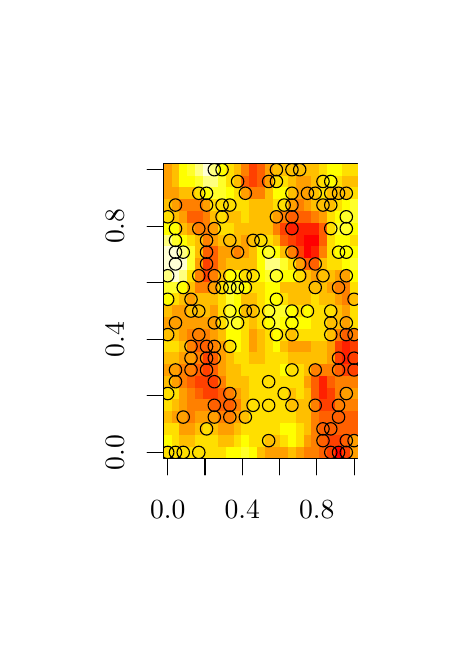
\begin{tikzpicture}[x=1pt,y=1pt]
\definecolor{fillColor}{RGB}{255,255,255}
\path[use as bounding box,fill=fillColor,fill opacity=0.00] (0,0) rectangle (144.54,216.81);
\begin{scope}
\path[clip] (  0.00,  0.00) rectangle (144.54,216.81);
\definecolor{drawColor}{RGB}{0,0,0}

\path[draw=drawColor,line width= 0.4pt,line join=round,line cap=round] ( 50.60, 61.20) -- (117.94, 61.20);

\path[draw=drawColor,line width= 0.4pt,line join=round,line cap=round] ( 50.60, 61.20) -- ( 50.60, 55.20);

\path[draw=drawColor,line width= 0.4pt,line join=round,line cap=round] ( 64.07, 61.20) -- ( 64.07, 55.20);

\path[draw=drawColor,line width= 0.4pt,line join=round,line cap=round] ( 77.54, 61.20) -- ( 77.54, 55.20);

\path[draw=drawColor,line width= 0.4pt,line join=round,line cap=round] ( 91.00, 61.20) -- ( 91.00, 55.20);

\path[draw=drawColor,line width= 0.4pt,line join=round,line cap=round] (104.47, 61.20) -- (104.47, 55.20);

\path[draw=drawColor,line width= 0.4pt,line join=round,line cap=round] (117.94, 61.20) -- (117.94, 55.20);

\node[text=drawColor,anchor=base,inner sep=0pt, outer sep=0pt, scale=  1.00] at ( 50.60, 39.60) {0.0};

\node[text=drawColor,anchor=base,inner sep=0pt, outer sep=0pt, scale=  1.00] at ( 77.54, 39.60) {0.4};

\node[text=drawColor,anchor=base,inner sep=0pt, outer sep=0pt, scale=  1.00] at (104.47, 39.60) {0.8};

\path[draw=drawColor,line width= 0.4pt,line join=round,line cap=round] ( 49.20, 63.33) -- ( 49.20,165.48);

\path[draw=drawColor,line width= 0.4pt,line join=round,line cap=round] ( 49.20, 63.33) -- ( 43.20, 63.33);

\path[draw=drawColor,line width= 0.4pt,line join=round,line cap=round] ( 49.20, 83.76) -- ( 43.20, 83.76);

\path[draw=drawColor,line width= 0.4pt,line join=round,line cap=round] ( 49.20,104.19) -- ( 43.20,104.19);

\path[draw=drawColor,line width= 0.4pt,line join=round,line cap=round] ( 49.20,124.62) -- ( 43.20,124.62);

\path[draw=drawColor,line width= 0.4pt,line join=round,line cap=round] ( 49.20,145.05) -- ( 43.20,145.05);

\path[draw=drawColor,line width= 0.4pt,line join=round,line cap=round] ( 49.20,165.48) -- ( 43.20,165.48);

\node[text=drawColor,rotate= 90.00,anchor=base,inner sep=0pt, outer sep=0pt, scale=  1.00] at ( 34.80, 63.33) {0.0};

\node[text=drawColor,rotate= 90.00,anchor=base,inner sep=0pt, outer sep=0pt, scale=  1.00] at ( 34.80,104.19) {0.4};

\node[text=drawColor,rotate= 90.00,anchor=base,inner sep=0pt, outer sep=0pt, scale=  1.00] at ( 34.80,145.05) {0.8};

\path[draw=drawColor,line width= 0.4pt,line join=round,line cap=round] ( 49.20, 61.20) --
	(119.34, 61.20) --
	(119.34,167.61) --
	( 49.20,167.61) --
	( 49.20, 61.20);
\end{scope}
\begin{scope}
\path[clip] ( 49.20, 61.20) rectangle (119.34,167.61);
\definecolor{fillColor}{RGB}{255,223,0}

\path[fill=fillColor] ( 49.20, 61.20) rectangle ( 52.01, 65.46);
\definecolor{fillColor}{RGB}{255,255,0}

\path[fill=fillColor] ( 49.20, 65.46) rectangle ( 52.01, 69.71);
\definecolor{fillColor}{RGB}{255,223,0}

\path[fill=fillColor] ( 49.20, 69.71) rectangle ( 52.01, 73.97);
\definecolor{fillColor}{RGB}{255,191,0}

\path[fill=fillColor] ( 49.20, 73.97) rectangle ( 52.01, 78.23);
\definecolor{fillColor}{RGB}{255,223,0}

\path[fill=fillColor] ( 49.20, 78.23) rectangle ( 52.01, 82.48);

\path[fill=fillColor] ( 49.20, 82.48) rectangle ( 52.01, 86.74);
\definecolor{fillColor}{RGB}{255,191,0}

\path[fill=fillColor] ( 49.20, 86.74) rectangle ( 52.01, 90.99);
\definecolor{fillColor}{RGB}{255,159,0}

\path[fill=fillColor] ( 49.20, 90.99) rectangle ( 52.01, 95.25);
\definecolor{fillColor}{RGB}{255,191,0}

\path[fill=fillColor] ( 49.20, 95.25) rectangle ( 52.01, 99.51);
\definecolor{fillColor}{RGB}{255,223,0}

\path[fill=fillColor] ( 49.20, 99.51) rectangle ( 52.01,103.76);
\definecolor{fillColor}{RGB}{255,191,0}

\path[fill=fillColor] ( 49.20,103.76) rectangle ( 52.01,108.02);
\definecolor{fillColor}{RGB}{255,159,0}

\path[fill=fillColor] ( 49.20,108.02) rectangle ( 52.01,112.28);
\definecolor{fillColor}{RGB}{255,191,0}

\path[fill=fillColor] ( 49.20,112.28) rectangle ( 52.01,116.53);
\definecolor{fillColor}{RGB}{255,255,0}

\path[fill=fillColor] ( 49.20,116.53) rectangle ( 52.01,120.79);
\definecolor{fillColor}{RGB}{255,255,42}

\path[fill=fillColor] ( 49.20,120.79) rectangle ( 52.01,125.05);
\definecolor{fillColor}{RGB}{255,255,128}

\path[fill=fillColor] ( 49.20,125.05) rectangle ( 52.01,129.30);
\definecolor{fillColor}{RGB}{255,255,213}

\path[fill=fillColor] ( 49.20,129.30) rectangle ( 52.01,133.56);

\path[fill=fillColor] ( 49.20,133.56) rectangle ( 52.01,137.82);
\definecolor{fillColor}{RGB}{255,255,128}

\path[fill=fillColor] ( 49.20,137.82) rectangle ( 52.01,142.07);
\definecolor{fillColor}{RGB}{255,255,0}

\path[fill=fillColor] ( 49.20,142.07) rectangle ( 52.01,146.33);
\definecolor{fillColor}{RGB}{255,223,0}

\path[fill=fillColor] ( 49.20,146.33) rectangle ( 52.01,150.58);
\definecolor{fillColor}{RGB}{255,191,0}

\path[fill=fillColor] ( 49.20,150.58) rectangle ( 52.01,154.84);
\definecolor{fillColor}{RGB}{255,159,0}

\path[fill=fillColor] ( 49.20,154.84) rectangle ( 52.01,159.10);

\path[fill=fillColor] ( 49.20,159.10) rectangle ( 52.01,163.35);

\path[fill=fillColor] ( 49.20,163.35) rectangle ( 52.01,167.61);
\definecolor{fillColor}{RGB}{255,223,0}

\path[fill=fillColor] ( 52.01, 61.20) rectangle ( 54.81, 65.46);

\path[fill=fillColor] ( 52.01, 65.46) rectangle ( 54.81, 69.71);

\path[fill=fillColor] ( 52.01, 69.71) rectangle ( 54.81, 73.97);
\definecolor{fillColor}{RGB}{255,159,0}

\path[fill=fillColor] ( 52.01, 73.97) rectangle ( 54.81, 78.23);
\definecolor{fillColor}{RGB}{255,191,0}

\path[fill=fillColor] ( 52.01, 78.23) rectangle ( 54.81, 82.48);
\definecolor{fillColor}{RGB}{255,223,0}

\path[fill=fillColor] ( 52.01, 82.48) rectangle ( 54.81, 86.74);
\definecolor{fillColor}{RGB}{255,159,0}

\path[fill=fillColor] ( 52.01, 86.74) rectangle ( 54.81, 90.99);

\path[fill=fillColor] ( 52.01, 90.99) rectangle ( 54.81, 95.25);
\definecolor{fillColor}{RGB}{255,191,0}

\path[fill=fillColor] ( 52.01, 95.25) rectangle ( 54.81, 99.51);
\definecolor{fillColor}{RGB}{255,223,0}

\path[fill=fillColor] ( 52.01, 99.51) rectangle ( 54.81,103.76);
\definecolor{fillColor}{RGB}{255,191,0}

\path[fill=fillColor] ( 52.01,103.76) rectangle ( 54.81,108.02);
\definecolor{fillColor}{RGB}{255,159,0}

\path[fill=fillColor] ( 52.01,108.02) rectangle ( 54.81,112.28);

\path[fill=fillColor] ( 52.01,112.28) rectangle ( 54.81,116.53);
\definecolor{fillColor}{RGB}{255,223,0}

\path[fill=fillColor] ( 52.01,116.53) rectangle ( 54.81,120.79);
\definecolor{fillColor}{RGB}{255,255,42}

\path[fill=fillColor] ( 52.01,120.79) rectangle ( 54.81,125.05);
\definecolor{fillColor}{RGB}{255,255,213}

\path[fill=fillColor] ( 52.01,125.05) rectangle ( 54.81,129.30);

\path[fill=fillColor] ( 52.01,129.30) rectangle ( 54.81,133.56);

\path[fill=fillColor] ( 52.01,133.56) rectangle ( 54.81,137.82);
\definecolor{fillColor}{RGB}{255,255,42}

\path[fill=fillColor] ( 52.01,137.82) rectangle ( 54.81,142.07);
\definecolor{fillColor}{RGB}{255,255,0}

\path[fill=fillColor] ( 52.01,142.07) rectangle ( 54.81,146.33);
\definecolor{fillColor}{RGB}{255,191,0}

\path[fill=fillColor] ( 52.01,146.33) rectangle ( 54.81,150.58);
\definecolor{fillColor}{RGB}{255,159,0}

\path[fill=fillColor] ( 52.01,150.58) rectangle ( 54.81,154.84);

\path[fill=fillColor] ( 52.01,154.84) rectangle ( 54.81,159.10);
\definecolor{fillColor}{RGB}{255,191,0}

\path[fill=fillColor] ( 52.01,159.10) rectangle ( 54.81,163.35);

\path[fill=fillColor] ( 52.01,163.35) rectangle ( 54.81,167.61);
\definecolor{fillColor}{RGB}{255,223,0}

\path[fill=fillColor] ( 54.81, 61.20) rectangle ( 57.62, 65.46);
\definecolor{fillColor}{RGB}{255,191,0}

\path[fill=fillColor] ( 54.81, 65.46) rectangle ( 57.62, 69.71);
\definecolor{fillColor}{RGB}{255,159,0}

\path[fill=fillColor] ( 54.81, 69.71) rectangle ( 57.62, 73.97);

\path[fill=fillColor] ( 54.81, 73.97) rectangle ( 57.62, 78.23);

\path[fill=fillColor] ( 54.81, 78.23) rectangle ( 57.62, 82.48);

\path[fill=fillColor] ( 54.81, 82.48) rectangle ( 57.62, 86.74);
\definecolor{fillColor}{RGB}{255,128,0}

\path[fill=fillColor] ( 54.81, 86.74) rectangle ( 57.62, 90.99);

\path[fill=fillColor] ( 54.81, 90.99) rectangle ( 57.62, 95.25);
\definecolor{fillColor}{RGB}{255,159,0}

\path[fill=fillColor] ( 54.81, 95.25) rectangle ( 57.62, 99.51);
\definecolor{fillColor}{RGB}{255,191,0}

\path[fill=fillColor] ( 54.81, 99.51) rectangle ( 57.62,103.76);
\definecolor{fillColor}{RGB}{255,159,0}

\path[fill=fillColor] ( 54.81,103.76) rectangle ( 57.62,108.02);

\path[fill=fillColor] ( 54.81,108.02) rectangle ( 57.62,112.28);

\path[fill=fillColor] ( 54.81,112.28) rectangle ( 57.62,116.53);
\definecolor{fillColor}{RGB}{255,191,0}

\path[fill=fillColor] ( 54.81,116.53) rectangle ( 57.62,120.79);
\definecolor{fillColor}{RGB}{255,255,0}

\path[fill=fillColor] ( 54.81,120.79) rectangle ( 57.62,125.05);
\definecolor{fillColor}{RGB}{255,255,128}

\path[fill=fillColor] ( 54.81,125.05) rectangle ( 57.62,129.30);
\definecolor{fillColor}{RGB}{255,255,213}

\path[fill=fillColor] ( 54.81,129.30) rectangle ( 57.62,133.56);
\definecolor{fillColor}{RGB}{255,255,128}

\path[fill=fillColor] ( 54.81,133.56) rectangle ( 57.62,137.82);
\definecolor{fillColor}{RGB}{255,255,0}

\path[fill=fillColor] ( 54.81,137.82) rectangle ( 57.62,142.07);
\definecolor{fillColor}{RGB}{255,191,0}

\path[fill=fillColor] ( 54.81,142.07) rectangle ( 57.62,146.33);
\definecolor{fillColor}{RGB}{255,159,0}

\path[fill=fillColor] ( 54.81,146.33) rectangle ( 57.62,150.58);
\definecolor{fillColor}{RGB}{255,128,0}

\path[fill=fillColor] ( 54.81,150.58) rectangle ( 57.62,154.84);
\definecolor{fillColor}{RGB}{255,191,0}

\path[fill=fillColor] ( 54.81,154.84) rectangle ( 57.62,159.10);
\definecolor{fillColor}{RGB}{255,255,0}

\path[fill=fillColor] ( 54.81,159.10) rectangle ( 57.62,163.35);

\path[fill=fillColor] ( 54.81,163.35) rectangle ( 57.62,167.61);
\definecolor{fillColor}{RGB}{255,223,0}

\path[fill=fillColor] ( 57.62, 61.20) rectangle ( 60.42, 65.46);
\definecolor{fillColor}{RGB}{255,191,0}

\path[fill=fillColor] ( 57.62, 65.46) rectangle ( 60.42, 69.71);
\definecolor{fillColor}{RGB}{255,159,0}

\path[fill=fillColor] ( 57.62, 69.71) rectangle ( 60.42, 73.97);
\definecolor{fillColor}{RGB}{255,128,0}

\path[fill=fillColor] ( 57.62, 73.97) rectangle ( 60.42, 78.23);

\path[fill=fillColor] ( 57.62, 78.23) rectangle ( 60.42, 82.48);

\path[fill=fillColor] ( 57.62, 82.48) rectangle ( 60.42, 86.74);
\definecolor{fillColor}{RGB}{255,96,0}

\path[fill=fillColor] ( 57.62, 86.74) rectangle ( 60.42, 90.99);
\definecolor{fillColor}{RGB}{255,128,0}

\path[fill=fillColor] ( 57.62, 90.99) rectangle ( 60.42, 95.25);
\definecolor{fillColor}{RGB}{255,159,0}

\path[fill=fillColor] ( 57.62, 95.25) rectangle ( 60.42, 99.51);
\definecolor{fillColor}{RGB}{255,128,0}

\path[fill=fillColor] ( 57.62, 99.51) rectangle ( 60.42,103.76);

\path[fill=fillColor] ( 57.62,103.76) rectangle ( 60.42,108.02);
\definecolor{fillColor}{RGB}{255,159,0}

\path[fill=fillColor] ( 57.62,108.02) rectangle ( 60.42,112.28);
\definecolor{fillColor}{RGB}{255,191,0}

\path[fill=fillColor] ( 57.62,112.28) rectangle ( 60.42,116.53);
\definecolor{fillColor}{RGB}{255,159,0}

\path[fill=fillColor] ( 57.62,116.53) rectangle ( 60.42,120.79);
\definecolor{fillColor}{RGB}{255,191,0}

\path[fill=fillColor] ( 57.62,120.79) rectangle ( 60.42,125.05);
\definecolor{fillColor}{RGB}{255,223,0}

\path[fill=fillColor] ( 57.62,125.05) rectangle ( 60.42,129.30);
\definecolor{fillColor}{RGB}{255,255,42}

\path[fill=fillColor] ( 57.62,129.30) rectangle ( 60.42,133.56);

\path[fill=fillColor] ( 57.62,133.56) rectangle ( 60.42,137.82);
\definecolor{fillColor}{RGB}{255,223,0}

\path[fill=fillColor] ( 57.62,137.82) rectangle ( 60.42,142.07);
\definecolor{fillColor}{RGB}{255,159,0}

\path[fill=fillColor] ( 57.62,142.07) rectangle ( 60.42,146.33);
\definecolor{fillColor}{RGB}{255,96,0}

\path[fill=fillColor] ( 57.62,146.33) rectangle ( 60.42,150.58);
\definecolor{fillColor}{RGB}{255,128,0}

\path[fill=fillColor] ( 57.62,150.58) rectangle ( 60.42,154.84);
\definecolor{fillColor}{RGB}{255,191,0}

\path[fill=fillColor] ( 57.62,154.84) rectangle ( 60.42,159.10);
\definecolor{fillColor}{RGB}{255,255,0}

\path[fill=fillColor] ( 57.62,159.10) rectangle ( 60.42,163.35);
\definecolor{fillColor}{RGB}{255,255,42}

\path[fill=fillColor] ( 57.62,163.35) rectangle ( 60.42,167.61);
\definecolor{fillColor}{RGB}{255,223,0}

\path[fill=fillColor] ( 60.42, 61.20) rectangle ( 63.23, 65.46);

\path[fill=fillColor] ( 60.42, 65.46) rectangle ( 63.23, 69.71);
\definecolor{fillColor}{RGB}{255,191,0}

\path[fill=fillColor] ( 60.42, 69.71) rectangle ( 63.23, 73.97);
\definecolor{fillColor}{RGB}{255,159,0}

\path[fill=fillColor] ( 60.42, 73.97) rectangle ( 63.23, 78.23);
\definecolor{fillColor}{RGB}{255,128,0}

\path[fill=fillColor] ( 60.42, 78.23) rectangle ( 63.23, 82.48);
\definecolor{fillColor}{RGB}{255,96,0}

\path[fill=fillColor] ( 60.42, 82.48) rectangle ( 63.23, 86.74);
\definecolor{fillColor}{RGB}{255,64,0}

\path[fill=fillColor] ( 60.42, 86.74) rectangle ( 63.23, 90.99);
\definecolor{fillColor}{RGB}{255,96,0}

\path[fill=fillColor] ( 60.42, 90.99) rectangle ( 63.23, 95.25);
\definecolor{fillColor}{RGB}{255,128,0}

\path[fill=fillColor] ( 60.42, 95.25) rectangle ( 63.23, 99.51);
\definecolor{fillColor}{RGB}{255,96,0}

\path[fill=fillColor] ( 60.42, 99.51) rectangle ( 63.23,103.76);
\definecolor{fillColor}{RGB}{255,128,0}

\path[fill=fillColor] ( 60.42,103.76) rectangle ( 63.23,108.02);
\definecolor{fillColor}{RGB}{255,159,0}

\path[fill=fillColor] ( 60.42,108.02) rectangle ( 63.23,112.28);
\definecolor{fillColor}{RGB}{255,191,0}

\path[fill=fillColor] ( 60.42,112.28) rectangle ( 63.23,116.53);

\path[fill=fillColor] ( 60.42,116.53) rectangle ( 63.23,120.79);
\definecolor{fillColor}{RGB}{255,128,0}

\path[fill=fillColor] ( 60.42,120.79) rectangle ( 63.23,125.05);

\path[fill=fillColor] ( 60.42,125.05) rectangle ( 63.23,129.30);
\definecolor{fillColor}{RGB}{255,159,0}

\path[fill=fillColor] ( 60.42,129.30) rectangle ( 63.23,133.56);
\definecolor{fillColor}{RGB}{255,191,0}

\path[fill=fillColor] ( 60.42,133.56) rectangle ( 63.23,137.82);

\path[fill=fillColor] ( 60.42,137.82) rectangle ( 63.23,142.07);
\definecolor{fillColor}{RGB}{255,128,0}

\path[fill=fillColor] ( 60.42,142.07) rectangle ( 63.23,146.33);
\definecolor{fillColor}{RGB}{255,96,0}

\path[fill=fillColor] ( 60.42,146.33) rectangle ( 63.23,150.58);
\definecolor{fillColor}{RGB}{255,128,0}

\path[fill=fillColor] ( 60.42,150.58) rectangle ( 63.23,154.84);
\definecolor{fillColor}{RGB}{255,223,0}

\path[fill=fillColor] ( 60.42,154.84) rectangle ( 63.23,159.10);
\definecolor{fillColor}{RGB}{255,255,42}

\path[fill=fillColor] ( 60.42,159.10) rectangle ( 63.23,163.35);
\definecolor{fillColor}{RGB}{255,255,128}

\path[fill=fillColor] ( 60.42,163.35) rectangle ( 63.23,167.61);
\definecolor{fillColor}{RGB}{255,223,0}

\path[fill=fillColor] ( 63.23, 61.20) rectangle ( 66.03, 65.46);

\path[fill=fillColor] ( 63.23, 65.46) rectangle ( 66.03, 69.71);

\path[fill=fillColor] ( 63.23, 69.71) rectangle ( 66.03, 73.97);
\definecolor{fillColor}{RGB}{255,159,0}

\path[fill=fillColor] ( 63.23, 73.97) rectangle ( 66.03, 78.23);
\definecolor{fillColor}{RGB}{255,128,0}

\path[fill=fillColor] ( 63.23, 78.23) rectangle ( 66.03, 82.48);
\definecolor{fillColor}{RGB}{255,64,0}

\path[fill=fillColor] ( 63.23, 82.48) rectangle ( 66.03, 86.74);

\path[fill=fillColor] ( 63.23, 86.74) rectangle ( 66.03, 90.99);

\path[fill=fillColor] ( 63.23, 90.99) rectangle ( 66.03, 95.25);

\path[fill=fillColor] ( 63.23, 95.25) rectangle ( 66.03, 99.51);
\definecolor{fillColor}{RGB}{255,96,0}

\path[fill=fillColor] ( 63.23, 99.51) rectangle ( 66.03,103.76);
\definecolor{fillColor}{RGB}{255,128,0}

\path[fill=fillColor] ( 63.23,103.76) rectangle ( 66.03,108.02);
\definecolor{fillColor}{RGB}{255,159,0}

\path[fill=fillColor] ( 63.23,108.02) rectangle ( 66.03,112.28);
\definecolor{fillColor}{RGB}{255,191,0}

\path[fill=fillColor] ( 63.23,112.28) rectangle ( 66.03,116.53);

\path[fill=fillColor] ( 63.23,116.53) rectangle ( 66.03,120.79);
\definecolor{fillColor}{RGB}{255,128,0}

\path[fill=fillColor] ( 63.23,120.79) rectangle ( 66.03,125.05);
\definecolor{fillColor}{RGB}{255,64,0}

\path[fill=fillColor] ( 63.23,125.05) rectangle ( 66.03,129.30);

\path[fill=fillColor] ( 63.23,129.30) rectangle ( 66.03,133.56);
\definecolor{fillColor}{RGB}{255,96,0}

\path[fill=fillColor] ( 63.23,133.56) rectangle ( 66.03,137.82);
\definecolor{fillColor}{RGB}{255,128,0}

\path[fill=fillColor] ( 63.23,137.82) rectangle ( 66.03,142.07);

\path[fill=fillColor] ( 63.23,142.07) rectangle ( 66.03,146.33);

\path[fill=fillColor] ( 63.23,146.33) rectangle ( 66.03,150.58);
\definecolor{fillColor}{RGB}{255,159,0}

\path[fill=fillColor] ( 63.23,150.58) rectangle ( 66.03,154.84);
\definecolor{fillColor}{RGB}{255,255,0}

\path[fill=fillColor] ( 63.23,154.84) rectangle ( 66.03,159.10);
\definecolor{fillColor}{RGB}{255,255,128}

\path[fill=fillColor] ( 63.23,159.10) rectangle ( 66.03,163.35);
\definecolor{fillColor}{RGB}{255,255,213}

\path[fill=fillColor] ( 63.23,163.35) rectangle ( 66.03,167.61);
\definecolor{fillColor}{RGB}{255,223,0}

\path[fill=fillColor] ( 66.03, 61.20) rectangle ( 68.84, 65.46);

\path[fill=fillColor] ( 66.03, 65.46) rectangle ( 68.84, 69.71);
\definecolor{fillColor}{RGB}{255,191,0}

\path[fill=fillColor] ( 66.03, 69.71) rectangle ( 68.84, 73.97);
\definecolor{fillColor}{RGB}{255,159,0}

\path[fill=fillColor] ( 66.03, 73.97) rectangle ( 68.84, 78.23);
\definecolor{fillColor}{RGB}{255,96,0}

\path[fill=fillColor] ( 66.03, 78.23) rectangle ( 68.84, 82.48);
\definecolor{fillColor}{RGB}{255,64,0}

\path[fill=fillColor] ( 66.03, 82.48) rectangle ( 68.84, 86.74);

\path[fill=fillColor] ( 66.03, 86.74) rectangle ( 68.84, 90.99);
\definecolor{fillColor}{RGB}{255,96,0}

\path[fill=fillColor] ( 66.03, 90.99) rectangle ( 68.84, 95.25);

\path[fill=fillColor] ( 66.03, 95.25) rectangle ( 68.84, 99.51);
\definecolor{fillColor}{RGB}{255,128,0}

\path[fill=fillColor] ( 66.03, 99.51) rectangle ( 68.84,103.76);
\definecolor{fillColor}{RGB}{255,159,0}

\path[fill=fillColor] ( 66.03,103.76) rectangle ( 68.84,108.02);

\path[fill=fillColor] ( 66.03,108.02) rectangle ( 68.84,112.28);

\path[fill=fillColor] ( 66.03,112.28) rectangle ( 68.84,116.53);
\definecolor{fillColor}{RGB}{255,191,0}

\path[fill=fillColor] ( 66.03,116.53) rectangle ( 68.84,120.79);
\definecolor{fillColor}{RGB}{255,159,0}

\path[fill=fillColor] ( 66.03,120.79) rectangle ( 68.84,125.05);
\definecolor{fillColor}{RGB}{255,128,0}

\path[fill=fillColor] ( 66.03,125.05) rectangle ( 68.84,129.30);
\definecolor{fillColor}{RGB}{255,96,0}

\path[fill=fillColor] ( 66.03,129.30) rectangle ( 68.84,133.56);

\path[fill=fillColor] ( 66.03,133.56) rectangle ( 68.84,137.82);
\definecolor{fillColor}{RGB}{255,159,0}

\path[fill=fillColor] ( 66.03,137.82) rectangle ( 68.84,142.07);

\path[fill=fillColor] ( 66.03,142.07) rectangle ( 68.84,146.33);
\definecolor{fillColor}{RGB}{255,191,0}

\path[fill=fillColor] ( 66.03,146.33) rectangle ( 68.84,150.58);
\definecolor{fillColor}{RGB}{255,223,0}

\path[fill=fillColor] ( 66.03,150.58) rectangle ( 68.84,154.84);
\definecolor{fillColor}{RGB}{255,255,42}

\path[fill=fillColor] ( 66.03,154.84) rectangle ( 68.84,159.10);
\definecolor{fillColor}{RGB}{255,255,128}

\path[fill=fillColor] ( 66.03,159.10) rectangle ( 68.84,163.35);

\path[fill=fillColor] ( 66.03,163.35) rectangle ( 68.84,167.61);
\definecolor{fillColor}{RGB}{255,223,0}

\path[fill=fillColor] ( 68.84, 61.20) rectangle ( 71.64, 65.46);
\definecolor{fillColor}{RGB}{255,191,0}

\path[fill=fillColor] ( 68.84, 65.46) rectangle ( 71.64, 69.71);
\definecolor{fillColor}{RGB}{255,159,0}

\path[fill=fillColor] ( 68.84, 69.71) rectangle ( 71.64, 73.97);
\definecolor{fillColor}{RGB}{255,128,0}

\path[fill=fillColor] ( 68.84, 73.97) rectangle ( 71.64, 78.23);
\definecolor{fillColor}{RGB}{255,96,0}

\path[fill=fillColor] ( 68.84, 78.23) rectangle ( 71.64, 82.48);

\path[fill=fillColor] ( 68.84, 82.48) rectangle ( 71.64, 86.74);
\definecolor{fillColor}{RGB}{255,128,0}

\path[fill=fillColor] ( 68.84, 86.74) rectangle ( 71.64, 90.99);
\definecolor{fillColor}{RGB}{255,159,0}

\path[fill=fillColor] ( 68.84, 90.99) rectangle ( 71.64, 95.25);

\path[fill=fillColor] ( 68.84, 95.25) rectangle ( 71.64, 99.51);

\path[fill=fillColor] ( 68.84, 99.51) rectangle ( 71.64,103.76);
\definecolor{fillColor}{RGB}{255,191,0}

\path[fill=fillColor] ( 68.84,103.76) rectangle ( 71.64,108.02);
\definecolor{fillColor}{RGB}{255,223,0}

\path[fill=fillColor] ( 68.84,108.02) rectangle ( 71.64,112.28);

\path[fill=fillColor] ( 68.84,112.28) rectangle ( 71.64,116.53);

\path[fill=fillColor] ( 68.84,116.53) rectangle ( 71.64,120.79);

\path[fill=fillColor] ( 68.84,120.79) rectangle ( 71.64,125.05);
\definecolor{fillColor}{RGB}{255,191,0}

\path[fill=fillColor] ( 68.84,125.05) rectangle ( 71.64,129.30);
\definecolor{fillColor}{RGB}{255,159,0}

\path[fill=fillColor] ( 68.84,129.30) rectangle ( 71.64,133.56);

\path[fill=fillColor] ( 68.84,133.56) rectangle ( 71.64,137.82);
\definecolor{fillColor}{RGB}{255,191,0}

\path[fill=fillColor] ( 68.84,137.82) rectangle ( 71.64,142.07);
\definecolor{fillColor}{RGB}{255,223,0}

\path[fill=fillColor] ( 68.84,142.07) rectangle ( 71.64,146.33);

\path[fill=fillColor] ( 68.84,146.33) rectangle ( 71.64,150.58);

\path[fill=fillColor] ( 68.84,150.58) rectangle ( 71.64,154.84);
\definecolor{fillColor}{RGB}{255,255,42}

\path[fill=fillColor] ( 68.84,154.84) rectangle ( 71.64,159.10);

\path[fill=fillColor] ( 68.84,159.10) rectangle ( 71.64,163.35);
\definecolor{fillColor}{RGB}{255,255,0}

\path[fill=fillColor] ( 68.84,163.35) rectangle ( 71.64,167.61);

\path[fill=fillColor] ( 71.64, 61.20) rectangle ( 74.45, 65.46);
\definecolor{fillColor}{RGB}{255,191,0}

\path[fill=fillColor] ( 71.64, 65.46) rectangle ( 74.45, 69.71);
\definecolor{fillColor}{RGB}{255,159,0}

\path[fill=fillColor] ( 71.64, 69.71) rectangle ( 74.45, 73.97);
\definecolor{fillColor}{RGB}{255,128,0}

\path[fill=fillColor] ( 71.64, 73.97) rectangle ( 74.45, 78.23);
\definecolor{fillColor}{RGB}{255,96,0}

\path[fill=fillColor] ( 71.64, 78.23) rectangle ( 74.45, 82.48);
\definecolor{fillColor}{RGB}{255,128,0}

\path[fill=fillColor] ( 71.64, 82.48) rectangle ( 74.45, 86.74);
\definecolor{fillColor}{RGB}{255,191,0}

\path[fill=fillColor] ( 71.64, 86.74) rectangle ( 74.45, 90.99);

\path[fill=fillColor] ( 71.64, 90.99) rectangle ( 74.45, 95.25);

\path[fill=fillColor] ( 71.64, 95.25) rectangle ( 74.45, 99.51);
\definecolor{fillColor}{RGB}{255,223,0}

\path[fill=fillColor] ( 71.64, 99.51) rectangle ( 74.45,103.76);
\definecolor{fillColor}{RGB}{255,255,0}

\path[fill=fillColor] ( 71.64,103.76) rectangle ( 74.45,108.02);
\definecolor{fillColor}{RGB}{255,255,42}

\path[fill=fillColor] ( 71.64,108.02) rectangle ( 74.45,112.28);

\path[fill=fillColor] ( 71.64,112.28) rectangle ( 74.45,116.53);

\path[fill=fillColor] ( 71.64,116.53) rectangle ( 74.45,120.79);

\path[fill=fillColor] ( 71.64,120.79) rectangle ( 74.45,125.05);
\definecolor{fillColor}{RGB}{255,255,0}

\path[fill=fillColor] ( 71.64,125.05) rectangle ( 74.45,129.30);
\definecolor{fillColor}{RGB}{255,191,0}

\path[fill=fillColor] ( 71.64,129.30) rectangle ( 74.45,133.56);
\definecolor{fillColor}{RGB}{255,159,0}

\path[fill=fillColor] ( 71.64,133.56) rectangle ( 74.45,137.82);
\definecolor{fillColor}{RGB}{255,191,0}

\path[fill=fillColor] ( 71.64,137.82) rectangle ( 74.45,142.07);
\definecolor{fillColor}{RGB}{255,223,0}

\path[fill=fillColor] ( 71.64,142.07) rectangle ( 74.45,146.33);
\definecolor{fillColor}{RGB}{255,191,0}

\path[fill=fillColor] ( 71.64,146.33) rectangle ( 74.45,150.58);
\definecolor{fillColor}{RGB}{255,223,0}

\path[fill=fillColor] ( 71.64,150.58) rectangle ( 74.45,154.84);
\definecolor{fillColor}{RGB}{255,255,0}

\path[fill=fillColor] ( 71.64,154.84) rectangle ( 74.45,159.10);
\definecolor{fillColor}{RGB}{255,223,0}

\path[fill=fillColor] ( 71.64,159.10) rectangle ( 74.45,163.35);

\path[fill=fillColor] ( 71.64,163.35) rectangle ( 74.45,167.61);
\definecolor{fillColor}{RGB}{255,255,0}

\path[fill=fillColor] ( 74.45, 61.20) rectangle ( 77.26, 65.46);
\definecolor{fillColor}{RGB}{255,223,0}

\path[fill=fillColor] ( 74.45, 65.46) rectangle ( 77.26, 69.71);
\definecolor{fillColor}{RGB}{255,191,0}

\path[fill=fillColor] ( 74.45, 69.71) rectangle ( 77.26, 73.97);
\definecolor{fillColor}{RGB}{255,159,0}

\path[fill=fillColor] ( 74.45, 73.97) rectangle ( 77.26, 78.23);
\definecolor{fillColor}{RGB}{255,128,0}

\path[fill=fillColor] ( 74.45, 78.23) rectangle ( 77.26, 82.48);
\definecolor{fillColor}{RGB}{255,159,0}

\path[fill=fillColor] ( 74.45, 82.48) rectangle ( 77.26, 86.74);
\definecolor{fillColor}{RGB}{255,191,0}

\path[fill=fillColor] ( 74.45, 86.74) rectangle ( 77.26, 90.99);

\path[fill=fillColor] ( 74.45, 90.99) rectangle ( 77.26, 95.25);
\definecolor{fillColor}{RGB}{255,223,0}

\path[fill=fillColor] ( 74.45, 95.25) rectangle ( 77.26, 99.51);
\definecolor{fillColor}{RGB}{255,255,0}

\path[fill=fillColor] ( 74.45, 99.51) rectangle ( 77.26,103.76);

\path[fill=fillColor] ( 74.45,103.76) rectangle ( 77.26,108.02);
\definecolor{fillColor}{RGB}{255,255,42}

\path[fill=fillColor] ( 74.45,108.02) rectangle ( 77.26,112.28);
\definecolor{fillColor}{RGB}{255,255,0}

\path[fill=fillColor] ( 74.45,112.28) rectangle ( 77.26,116.53);

\path[fill=fillColor] ( 74.45,116.53) rectangle ( 77.26,120.79);
\definecolor{fillColor}{RGB}{255,255,42}

\path[fill=fillColor] ( 74.45,120.79) rectangle ( 77.26,125.05);
\definecolor{fillColor}{RGB}{255,255,0}

\path[fill=fillColor] ( 74.45,125.05) rectangle ( 77.26,129.30);
\definecolor{fillColor}{RGB}{255,191,0}

\path[fill=fillColor] ( 74.45,129.30) rectangle ( 77.26,133.56);
\definecolor{fillColor}{RGB}{255,128,0}

\path[fill=fillColor] ( 74.45,133.56) rectangle ( 77.26,137.82);
\definecolor{fillColor}{RGB}{255,191,0}

\path[fill=fillColor] ( 74.45,137.82) rectangle ( 77.26,142.07);

\path[fill=fillColor] ( 74.45,142.07) rectangle ( 77.26,146.33);

\path[fill=fillColor] ( 74.45,146.33) rectangle ( 77.26,150.58);
\definecolor{fillColor}{RGB}{255,223,0}

\path[fill=fillColor] ( 74.45,150.58) rectangle ( 77.26,154.84);

\path[fill=fillColor] ( 74.45,154.84) rectangle ( 77.26,159.10);
\definecolor{fillColor}{RGB}{255,191,0}

\path[fill=fillColor] ( 74.45,159.10) rectangle ( 77.26,163.35);

\path[fill=fillColor] ( 74.45,163.35) rectangle ( 77.26,167.61);
\definecolor{fillColor}{RGB}{255,255,42}

\path[fill=fillColor] ( 77.26, 61.20) rectangle ( 80.06, 65.46);
\definecolor{fillColor}{RGB}{255,255,0}

\path[fill=fillColor] ( 77.26, 65.46) rectangle ( 80.06, 69.71);
\definecolor{fillColor}{RGB}{255,223,0}

\path[fill=fillColor] ( 77.26, 69.71) rectangle ( 80.06, 73.97);
\definecolor{fillColor}{RGB}{255,191,0}

\path[fill=fillColor] ( 77.26, 73.97) rectangle ( 80.06, 78.23);

\path[fill=fillColor] ( 77.26, 78.23) rectangle ( 80.06, 82.48);

\path[fill=fillColor] ( 77.26, 82.48) rectangle ( 80.06, 86.74);

\path[fill=fillColor] ( 77.26, 86.74) rectangle ( 80.06, 90.99);
\definecolor{fillColor}{RGB}{255,223,0}

\path[fill=fillColor] ( 77.26, 90.99) rectangle ( 80.06, 95.25);

\path[fill=fillColor] ( 77.26, 95.25) rectangle ( 80.06, 99.51);

\path[fill=fillColor] ( 77.26, 99.51) rectangle ( 80.06,103.76);

\path[fill=fillColor] ( 77.26,103.76) rectangle ( 80.06,108.02);

\path[fill=fillColor] ( 77.26,108.02) rectangle ( 80.06,112.28);
\definecolor{fillColor}{RGB}{255,191,0}

\path[fill=fillColor] ( 77.26,112.28) rectangle ( 80.06,116.53);

\path[fill=fillColor] ( 77.26,116.53) rectangle ( 80.06,120.79);
\definecolor{fillColor}{RGB}{255,255,0}

\path[fill=fillColor] ( 77.26,120.79) rectangle ( 80.06,125.05);
\definecolor{fillColor}{RGB}{255,223,0}

\path[fill=fillColor] ( 77.26,125.05) rectangle ( 80.06,129.30);
\definecolor{fillColor}{RGB}{255,191,0}

\path[fill=fillColor] ( 77.26,129.30) rectangle ( 80.06,133.56);
\definecolor{fillColor}{RGB}{255,159,0}

\path[fill=fillColor] ( 77.26,133.56) rectangle ( 80.06,137.82);

\path[fill=fillColor] ( 77.26,137.82) rectangle ( 80.06,142.07);
\definecolor{fillColor}{RGB}{255,191,0}

\path[fill=fillColor] ( 77.26,142.07) rectangle ( 80.06,146.33);
\definecolor{fillColor}{RGB}{255,223,0}

\path[fill=fillColor] ( 77.26,146.33) rectangle ( 80.06,150.58);

\path[fill=fillColor] ( 77.26,150.58) rectangle ( 80.06,154.84);
\definecolor{fillColor}{RGB}{255,159,0}

\path[fill=fillColor] ( 77.26,154.84) rectangle ( 80.06,159.10);
\definecolor{fillColor}{RGB}{255,96,0}

\path[fill=fillColor] ( 77.26,159.10) rectangle ( 80.06,163.35);
\definecolor{fillColor}{RGB}{255,128,0}

\path[fill=fillColor] ( 77.26,163.35) rectangle ( 80.06,167.61);
\definecolor{fillColor}{RGB}{255,255,0}

\path[fill=fillColor] ( 80.06, 61.20) rectangle ( 82.87, 65.46);
\definecolor{fillColor}{RGB}{255,223,0}

\path[fill=fillColor] ( 80.06, 65.46) rectangle ( 82.87, 69.71);

\path[fill=fillColor] ( 80.06, 69.71) rectangle ( 82.87, 73.97);

\path[fill=fillColor] ( 80.06, 73.97) rectangle ( 82.87, 78.23);

\path[fill=fillColor] ( 80.06, 78.23) rectangle ( 82.87, 82.48);

\path[fill=fillColor] ( 80.06, 82.48) rectangle ( 82.87, 86.74);

\path[fill=fillColor] ( 80.06, 86.74) rectangle ( 82.87, 90.99);

\path[fill=fillColor] ( 80.06, 90.99) rectangle ( 82.87, 95.25);
\definecolor{fillColor}{RGB}{255,191,0}

\path[fill=fillColor] ( 80.06, 95.25) rectangle ( 82.87, 99.51);
\definecolor{fillColor}{RGB}{255,159,0}

\path[fill=fillColor] ( 80.06, 99.51) rectangle ( 82.87,103.76);

\path[fill=fillColor] ( 80.06,103.76) rectangle ( 82.87,108.02);
\definecolor{fillColor}{RGB}{255,191,0}

\path[fill=fillColor] ( 80.06,108.02) rectangle ( 82.87,112.28);

\path[fill=fillColor] ( 80.06,112.28) rectangle ( 82.87,116.53);

\path[fill=fillColor] ( 80.06,116.53) rectangle ( 82.87,120.79);
\definecolor{fillColor}{RGB}{255,223,0}

\path[fill=fillColor] ( 80.06,120.79) rectangle ( 82.87,125.05);

\path[fill=fillColor] ( 80.06,125.05) rectangle ( 82.87,129.30);
\definecolor{fillColor}{RGB}{255,191,0}

\path[fill=fillColor] ( 80.06,129.30) rectangle ( 82.87,133.56);

\path[fill=fillColor] ( 80.06,133.56) rectangle ( 82.87,137.82);

\path[fill=fillColor] ( 80.06,137.82) rectangle ( 82.87,142.07);

\path[fill=fillColor] ( 80.06,142.07) rectangle ( 82.87,146.33);

\path[fill=fillColor] ( 80.06,146.33) rectangle ( 82.87,150.58);

\path[fill=fillColor] ( 80.06,150.58) rectangle ( 82.87,154.84);
\definecolor{fillColor}{RGB}{255,128,0}

\path[fill=fillColor] ( 80.06,154.84) rectangle ( 82.87,159.10);
\definecolor{fillColor}{RGB}{255,64,0}

\path[fill=fillColor] ( 80.06,159.10) rectangle ( 82.87,163.35);

\path[fill=fillColor] ( 80.06,163.35) rectangle ( 82.87,167.61);
\definecolor{fillColor}{RGB}{255,191,0}

\path[fill=fillColor] ( 82.87, 61.20) rectangle ( 85.67, 65.46);
\definecolor{fillColor}{RGB}{255,223,0}

\path[fill=fillColor] ( 82.87, 65.46) rectangle ( 85.67, 69.71);

\path[fill=fillColor] ( 82.87, 69.71) rectangle ( 85.67, 73.97);

\path[fill=fillColor] ( 82.87, 73.97) rectangle ( 85.67, 78.23);

\path[fill=fillColor] ( 82.87, 78.23) rectangle ( 85.67, 82.48);

\path[fill=fillColor] ( 82.87, 82.48) rectangle ( 85.67, 86.74);

\path[fill=fillColor] ( 82.87, 86.74) rectangle ( 85.67, 90.99);

\path[fill=fillColor] ( 82.87, 90.99) rectangle ( 85.67, 95.25);
\definecolor{fillColor}{RGB}{255,191,0}

\path[fill=fillColor] ( 82.87, 95.25) rectangle ( 85.67, 99.51);

\path[fill=fillColor] ( 82.87, 99.51) rectangle ( 85.67,103.76);

\path[fill=fillColor] ( 82.87,103.76) rectangle ( 85.67,108.02);
\definecolor{fillColor}{RGB}{255,223,0}

\path[fill=fillColor] ( 82.87,108.02) rectangle ( 85.67,112.28);

\path[fill=fillColor] ( 82.87,112.28) rectangle ( 85.67,116.53);

\path[fill=fillColor] ( 82.87,116.53) rectangle ( 85.67,120.79);

\path[fill=fillColor] ( 82.87,120.79) rectangle ( 85.67,125.05);
\definecolor{fillColor}{RGB}{255,255,0}

\path[fill=fillColor] ( 82.87,125.05) rectangle ( 85.67,129.30);

\path[fill=fillColor] ( 82.87,129.30) rectangle ( 85.67,133.56);

\path[fill=fillColor] ( 82.87,133.56) rectangle ( 85.67,137.82);
\definecolor{fillColor}{RGB}{255,223,0}

\path[fill=fillColor] ( 82.87,137.82) rectangle ( 85.67,142.07);
\definecolor{fillColor}{RGB}{255,191,0}

\path[fill=fillColor] ( 82.87,142.07) rectangle ( 85.67,146.33);

\path[fill=fillColor] ( 82.87,146.33) rectangle ( 85.67,150.58);

\path[fill=fillColor] ( 82.87,150.58) rectangle ( 85.67,154.84);
\definecolor{fillColor}{RGB}{255,128,0}

\path[fill=fillColor] ( 82.87,154.84) rectangle ( 85.67,159.10);
\definecolor{fillColor}{RGB}{255,96,0}

\path[fill=fillColor] ( 82.87,159.10) rectangle ( 85.67,163.35);

\path[fill=fillColor] ( 82.87,163.35) rectangle ( 85.67,167.61);
\definecolor{fillColor}{RGB}{255,159,0}

\path[fill=fillColor] ( 85.67, 61.20) rectangle ( 88.48, 65.46);
\definecolor{fillColor}{RGB}{255,191,0}

\path[fill=fillColor] ( 85.67, 65.46) rectangle ( 88.48, 69.71);
\definecolor{fillColor}{RGB}{255,223,0}

\path[fill=fillColor] ( 85.67, 69.71) rectangle ( 88.48, 73.97);

\path[fill=fillColor] ( 85.67, 73.97) rectangle ( 88.48, 78.23);

\path[fill=fillColor] ( 85.67, 78.23) rectangle ( 88.48, 82.48);

\path[fill=fillColor] ( 85.67, 82.48) rectangle ( 88.48, 86.74);

\path[fill=fillColor] ( 85.67, 86.74) rectangle ( 88.48, 90.99);

\path[fill=fillColor] ( 85.67, 90.99) rectangle ( 88.48, 95.25);

\path[fill=fillColor] ( 85.67, 95.25) rectangle ( 88.48, 99.51);

\path[fill=fillColor] ( 85.67, 99.51) rectangle ( 88.48,103.76);

\path[fill=fillColor] ( 85.67,103.76) rectangle ( 88.48,108.02);
\definecolor{fillColor}{RGB}{255,255,0}

\path[fill=fillColor] ( 85.67,108.02) rectangle ( 88.48,112.28);
\definecolor{fillColor}{RGB}{255,255,42}

\path[fill=fillColor] ( 85.67,112.28) rectangle ( 88.48,116.53);
\definecolor{fillColor}{RGB}{255,255,0}

\path[fill=fillColor] ( 85.67,116.53) rectangle ( 88.48,120.79);

\path[fill=fillColor] ( 85.67,120.79) rectangle ( 88.48,125.05);
\definecolor{fillColor}{RGB}{255,255,42}

\path[fill=fillColor] ( 85.67,125.05) rectangle ( 88.48,129.30);
\definecolor{fillColor}{RGB}{255,255,128}

\path[fill=fillColor] ( 85.67,129.30) rectangle ( 88.48,133.56);
\definecolor{fillColor}{RGB}{255,255,42}

\path[fill=fillColor] ( 85.67,133.56) rectangle ( 88.48,137.82);
\definecolor{fillColor}{RGB}{255,223,0}

\path[fill=fillColor] ( 85.67,137.82) rectangle ( 88.48,142.07);
\definecolor{fillColor}{RGB}{255,191,0}

\path[fill=fillColor] ( 85.67,142.07) rectangle ( 88.48,146.33);

\path[fill=fillColor] ( 85.67,146.33) rectangle ( 88.48,150.58);

\path[fill=fillColor] ( 85.67,150.58) rectangle ( 88.48,154.84);

\path[fill=fillColor] ( 85.67,154.84) rectangle ( 88.48,159.10);
\definecolor{fillColor}{RGB}{255,159,0}

\path[fill=fillColor] ( 85.67,159.10) rectangle ( 88.48,163.35);

\path[fill=fillColor] ( 85.67,163.35) rectangle ( 88.48,167.61);

\path[fill=fillColor] ( 88.48, 61.20) rectangle ( 91.28, 65.46);
\definecolor{fillColor}{RGB}{255,191,0}

\path[fill=fillColor] ( 88.48, 65.46) rectangle ( 91.28, 69.71);
\definecolor{fillColor}{RGB}{255,223,0}

\path[fill=fillColor] ( 88.48, 69.71) rectangle ( 91.28, 73.97);

\path[fill=fillColor] ( 88.48, 73.97) rectangle ( 91.28, 78.23);

\path[fill=fillColor] ( 88.48, 78.23) rectangle ( 91.28, 82.48);

\path[fill=fillColor] ( 88.48, 82.48) rectangle ( 91.28, 86.74);

\path[fill=fillColor] ( 88.48, 86.74) rectangle ( 91.28, 90.99);

\path[fill=fillColor] ( 88.48, 90.99) rectangle ( 91.28, 95.25);

\path[fill=fillColor] ( 88.48, 95.25) rectangle ( 91.28, 99.51);
\definecolor{fillColor}{RGB}{255,255,0}

\path[fill=fillColor] ( 88.48, 99.51) rectangle ( 91.28,103.76);

\path[fill=fillColor] ( 88.48,103.76) rectangle ( 91.28,108.02);
\definecolor{fillColor}{RGB}{255,255,42}

\path[fill=fillColor] ( 88.48,108.02) rectangle ( 91.28,112.28);

\path[fill=fillColor] ( 88.48,112.28) rectangle ( 91.28,116.53);
\definecolor{fillColor}{RGB}{255,255,0}

\path[fill=fillColor] ( 88.48,116.53) rectangle ( 91.28,120.79);

\path[fill=fillColor] ( 88.48,120.79) rectangle ( 91.28,125.05);
\definecolor{fillColor}{RGB}{255,255,42}

\path[fill=fillColor] ( 88.48,125.05) rectangle ( 91.28,129.30);
\definecolor{fillColor}{RGB}{255,255,128}

\path[fill=fillColor] ( 88.48,129.30) rectangle ( 91.28,133.56);
\definecolor{fillColor}{RGB}{255,255,0}

\path[fill=fillColor] ( 88.48,133.56) rectangle ( 91.28,137.82);
\definecolor{fillColor}{RGB}{255,191,0}

\path[fill=fillColor] ( 88.48,137.82) rectangle ( 91.28,142.07);
\definecolor{fillColor}{RGB}{255,128,0}

\path[fill=fillColor] ( 88.48,142.07) rectangle ( 91.28,146.33);
\definecolor{fillColor}{RGB}{255,159,0}

\path[fill=fillColor] ( 88.48,146.33) rectangle ( 91.28,150.58);
\definecolor{fillColor}{RGB}{255,223,0}

\path[fill=fillColor] ( 88.48,150.58) rectangle ( 91.28,154.84);
\definecolor{fillColor}{RGB}{255,255,0}

\path[fill=fillColor] ( 88.48,154.84) rectangle ( 91.28,159.10);
\definecolor{fillColor}{RGB}{255,223,0}

\path[fill=fillColor] ( 88.48,159.10) rectangle ( 91.28,163.35);
\definecolor{fillColor}{RGB}{255,191,0}

\path[fill=fillColor] ( 88.48,163.35) rectangle ( 91.28,167.61);
\definecolor{fillColor}{RGB}{255,159,0}

\path[fill=fillColor] ( 91.28, 61.20) rectangle ( 94.09, 65.46);
\definecolor{fillColor}{RGB}{255,223,0}

\path[fill=fillColor] ( 91.28, 65.46) rectangle ( 94.09, 69.71);
\definecolor{fillColor}{RGB}{255,255,0}

\path[fill=fillColor] ( 91.28, 69.71) rectangle ( 94.09, 73.97);
\definecolor{fillColor}{RGB}{255,223,0}

\path[fill=fillColor] ( 91.28, 73.97) rectangle ( 94.09, 78.23);

\path[fill=fillColor] ( 91.28, 78.23) rectangle ( 94.09, 82.48);

\path[fill=fillColor] ( 91.28, 82.48) rectangle ( 94.09, 86.74);

\path[fill=fillColor] ( 91.28, 86.74) rectangle ( 94.09, 90.99);
\definecolor{fillColor}{RGB}{255,255,0}

\path[fill=fillColor] ( 91.28, 90.99) rectangle ( 94.09, 95.25);
\definecolor{fillColor}{RGB}{255,223,0}

\path[fill=fillColor] ( 91.28, 95.25) rectangle ( 94.09, 99.51);
\definecolor{fillColor}{RGB}{255,191,0}

\path[fill=fillColor] ( 91.28, 99.51) rectangle ( 94.09,103.76);
\definecolor{fillColor}{RGB}{255,223,0}

\path[fill=fillColor] ( 91.28,103.76) rectangle ( 94.09,108.02);
\definecolor{fillColor}{RGB}{255,255,0}

\path[fill=fillColor] ( 91.28,108.02) rectangle ( 94.09,112.28);
\definecolor{fillColor}{RGB}{255,255,42}

\path[fill=fillColor] ( 91.28,112.28) rectangle ( 94.09,116.53);
\definecolor{fillColor}{RGB}{255,223,0}

\path[fill=fillColor] ( 91.28,116.53) rectangle ( 94.09,120.79);
\definecolor{fillColor}{RGB}{255,191,0}

\path[fill=fillColor] ( 91.28,120.79) rectangle ( 94.09,125.05);
\definecolor{fillColor}{RGB}{255,255,0}

\path[fill=fillColor] ( 91.28,125.05) rectangle ( 94.09,129.30);
\definecolor{fillColor}{RGB}{255,255,42}

\path[fill=fillColor] ( 91.28,129.30) rectangle ( 94.09,133.56);
\definecolor{fillColor}{RGB}{255,191,0}

\path[fill=fillColor] ( 91.28,133.56) rectangle ( 94.09,137.82);
\definecolor{fillColor}{RGB}{255,96,0}

\path[fill=fillColor] ( 91.28,137.82) rectangle ( 94.09,142.07);
\definecolor{fillColor}{RGB}{255,64,0}

\path[fill=fillColor] ( 91.28,142.07) rectangle ( 94.09,146.33);
\definecolor{fillColor}{RGB}{255,128,0}

\path[fill=fillColor] ( 91.28,146.33) rectangle ( 94.09,150.58);
\definecolor{fillColor}{RGB}{255,223,0}

\path[fill=fillColor] ( 91.28,150.58) rectangle ( 94.09,154.84);
\definecolor{fillColor}{RGB}{255,255,0}

\path[fill=fillColor] ( 91.28,154.84) rectangle ( 94.09,159.10);
\definecolor{fillColor}{RGB}{255,223,0}

\path[fill=fillColor] ( 91.28,159.10) rectangle ( 94.09,163.35);
\definecolor{fillColor}{RGB}{255,191,0}

\path[fill=fillColor] ( 91.28,163.35) rectangle ( 94.09,167.61);

\path[fill=fillColor] ( 94.09, 61.20) rectangle ( 96.90, 65.46);
\definecolor{fillColor}{RGB}{255,255,0}

\path[fill=fillColor] ( 94.09, 65.46) rectangle ( 96.90, 69.71);

\path[fill=fillColor] ( 94.09, 69.71) rectangle ( 96.90, 73.97);
\definecolor{fillColor}{RGB}{255,223,0}

\path[fill=fillColor] ( 94.09, 73.97) rectangle ( 96.90, 78.23);
\definecolor{fillColor}{RGB}{255,191,0}

\path[fill=fillColor] ( 94.09, 78.23) rectangle ( 96.90, 82.48);

\path[fill=fillColor] ( 94.09, 82.48) rectangle ( 96.90, 86.74);
\definecolor{fillColor}{RGB}{255,223,0}

\path[fill=fillColor] ( 94.09, 86.74) rectangle ( 96.90, 90.99);

\path[fill=fillColor] ( 94.09, 90.99) rectangle ( 96.90, 95.25);
\definecolor{fillColor}{RGB}{255,191,0}

\path[fill=fillColor] ( 94.09, 95.25) rectangle ( 96.90, 99.51);
\definecolor{fillColor}{RGB}{255,159,0}

\path[fill=fillColor] ( 94.09, 99.51) rectangle ( 96.90,103.76);
\definecolor{fillColor}{RGB}{255,191,0}

\path[fill=fillColor] ( 94.09,103.76) rectangle ( 96.90,108.02);
\definecolor{fillColor}{RGB}{255,255,0}

\path[fill=fillColor] ( 94.09,108.02) rectangle ( 96.90,112.28);

\path[fill=fillColor] ( 94.09,112.28) rectangle ( 96.90,116.53);
\definecolor{fillColor}{RGB}{255,191,0}

\path[fill=fillColor] ( 94.09,116.53) rectangle ( 96.90,120.79);

\path[fill=fillColor] ( 94.09,120.79) rectangle ( 96.90,125.05);
\definecolor{fillColor}{RGB}{255,255,0}

\path[fill=fillColor] ( 94.09,125.05) rectangle ( 96.90,129.30);
\definecolor{fillColor}{RGB}{255,223,0}

\path[fill=fillColor] ( 94.09,129.30) rectangle ( 96.90,133.56);
\definecolor{fillColor}{RGB}{255,128,0}

\path[fill=fillColor] ( 94.09,133.56) rectangle ( 96.90,137.82);
\definecolor{fillColor}{RGB}{255,64,0}

\path[fill=fillColor] ( 94.09,137.82) rectangle ( 96.90,142.07);
\definecolor{fillColor}{RGB}{255,32,0}

\path[fill=fillColor] ( 94.09,142.07) rectangle ( 96.90,146.33);
\definecolor{fillColor}{RGB}{255,96,0}

\path[fill=fillColor] ( 94.09,146.33) rectangle ( 96.90,150.58);
\definecolor{fillColor}{RGB}{255,159,0}

\path[fill=fillColor] ( 94.09,150.58) rectangle ( 96.90,154.84);
\definecolor{fillColor}{RGB}{255,191,0}

\path[fill=fillColor] ( 94.09,154.84) rectangle ( 96.90,159.10);

\path[fill=fillColor] ( 94.09,159.10) rectangle ( 96.90,163.35);

\path[fill=fillColor] ( 94.09,163.35) rectangle ( 96.90,167.61);
\definecolor{fillColor}{RGB}{255,159,0}

\path[fill=fillColor] ( 96.90, 61.20) rectangle ( 99.70, 65.46);
\definecolor{fillColor}{RGB}{255,223,0}

\path[fill=fillColor] ( 96.90, 65.46) rectangle ( 99.70, 69.71);

\path[fill=fillColor] ( 96.90, 69.71) rectangle ( 99.70, 73.97);
\definecolor{fillColor}{RGB}{255,191,0}

\path[fill=fillColor] ( 96.90, 73.97) rectangle ( 99.70, 78.23);

\path[fill=fillColor] ( 96.90, 78.23) rectangle ( 99.70, 82.48);
\definecolor{fillColor}{RGB}{255,223,0}

\path[fill=fillColor] ( 96.90, 82.48) rectangle ( 99.70, 86.74);

\path[fill=fillColor] ( 96.90, 86.74) rectangle ( 99.70, 90.99);

\path[fill=fillColor] ( 96.90, 90.99) rectangle ( 99.70, 95.25);
\definecolor{fillColor}{RGB}{255,191,0}

\path[fill=fillColor] ( 96.90, 95.25) rectangle ( 99.70, 99.51);
\definecolor{fillColor}{RGB}{255,159,0}

\path[fill=fillColor] ( 96.90, 99.51) rectangle ( 99.70,103.76);
\definecolor{fillColor}{RGB}{255,223,0}

\path[fill=fillColor] ( 96.90,103.76) rectangle ( 99.70,108.02);
\definecolor{fillColor}{RGB}{255,255,0}

\path[fill=fillColor] ( 96.90,108.02) rectangle ( 99.70,112.28);
\definecolor{fillColor}{RGB}{255,223,0}

\path[fill=fillColor] ( 96.90,112.28) rectangle ( 99.70,116.53);
\definecolor{fillColor}{RGB}{255,191,0}

\path[fill=fillColor] ( 96.90,116.53) rectangle ( 99.70,120.79);

\path[fill=fillColor] ( 96.90,120.79) rectangle ( 99.70,125.05);
\definecolor{fillColor}{RGB}{255,223,0}

\path[fill=fillColor] ( 96.90,125.05) rectangle ( 99.70,129.30);
\definecolor{fillColor}{RGB}{255,159,0}

\path[fill=fillColor] ( 96.90,129.30) rectangle ( 99.70,133.56);
\definecolor{fillColor}{RGB}{255,64,0}

\path[fill=fillColor] ( 96.90,133.56) rectangle ( 99.70,137.82);
\definecolor{fillColor}{RGB}{255,32,0}

\path[fill=fillColor] ( 96.90,137.82) rectangle ( 99.70,142.07);

\path[fill=fillColor] ( 96.90,142.07) rectangle ( 99.70,146.33);
\definecolor{fillColor}{RGB}{255,96,0}

\path[fill=fillColor] ( 96.90,146.33) rectangle ( 99.70,150.58);
\definecolor{fillColor}{RGB}{255,128,0}

\path[fill=fillColor] ( 96.90,150.58) rectangle ( 99.70,154.84);
\definecolor{fillColor}{RGB}{255,159,0}

\path[fill=fillColor] ( 96.90,154.84) rectangle ( 99.70,159.10);

\path[fill=fillColor] ( 96.90,159.10) rectangle ( 99.70,163.35);
\definecolor{fillColor}{RGB}{255,191,0}

\path[fill=fillColor] ( 96.90,163.35) rectangle ( 99.70,167.61);
\definecolor{fillColor}{RGB}{255,128,0}

\path[fill=fillColor] ( 99.70, 61.20) rectangle (102.51, 65.46);
\definecolor{fillColor}{RGB}{255,159,0}

\path[fill=fillColor] ( 99.70, 65.46) rectangle (102.51, 69.71);
\definecolor{fillColor}{RGB}{255,191,0}

\path[fill=fillColor] ( 99.70, 69.71) rectangle (102.51, 73.97);

\path[fill=fillColor] ( 99.70, 73.97) rectangle (102.51, 78.23);

\path[fill=fillColor] ( 99.70, 78.23) rectangle (102.51, 82.48);

\path[fill=fillColor] ( 99.70, 82.48) rectangle (102.51, 86.74);
\definecolor{fillColor}{RGB}{255,159,0}

\path[fill=fillColor] ( 99.70, 86.74) rectangle (102.51, 90.99);
\definecolor{fillColor}{RGB}{255,191,0}

\path[fill=fillColor] ( 99.70, 90.99) rectangle (102.51, 95.25);

\path[fill=fillColor] ( 99.70, 95.25) rectangle (102.51, 99.51);
\definecolor{fillColor}{RGB}{255,159,0}

\path[fill=fillColor] ( 99.70, 99.51) rectangle (102.51,103.76);
\definecolor{fillColor}{RGB}{255,223,0}

\path[fill=fillColor] ( 99.70,103.76) rectangle (102.51,108.02);
\definecolor{fillColor}{RGB}{255,255,0}

\path[fill=fillColor] ( 99.70,108.02) rectangle (102.51,112.28);

\path[fill=fillColor] ( 99.70,112.28) rectangle (102.51,116.53);
\definecolor{fillColor}{RGB}{255,191,0}

\path[fill=fillColor] ( 99.70,116.53) rectangle (102.51,120.79);

\path[fill=fillColor] ( 99.70,120.79) rectangle (102.51,125.05);

\path[fill=fillColor] ( 99.70,125.05) rectangle (102.51,129.30);
\definecolor{fillColor}{RGB}{255,96,0}

\path[fill=fillColor] ( 99.70,129.30) rectangle (102.51,133.56);
\definecolor{fillColor}{RGB}{255,0,0}

\path[fill=fillColor] ( 99.70,133.56) rectangle (102.51,137.82);

\path[fill=fillColor] ( 99.70,137.82) rectangle (102.51,142.07);
\definecolor{fillColor}{RGB}{255,32,0}

\path[fill=fillColor] ( 99.70,142.07) rectangle (102.51,146.33);
\definecolor{fillColor}{RGB}{255,96,0}

\path[fill=fillColor] ( 99.70,146.33) rectangle (102.51,150.58);
\definecolor{fillColor}{RGB}{255,159,0}

\path[fill=fillColor] ( 99.70,150.58) rectangle (102.51,154.84);

\path[fill=fillColor] ( 99.70,154.84) rectangle (102.51,159.10);

\path[fill=fillColor] ( 99.70,159.10) rectangle (102.51,163.35);
\definecolor{fillColor}{RGB}{255,191,0}

\path[fill=fillColor] ( 99.70,163.35) rectangle (102.51,167.61);
\definecolor{fillColor}{RGB}{255,128,0}

\path[fill=fillColor] (102.51, 61.20) rectangle (105.31, 65.46);

\path[fill=fillColor] (102.51, 65.46) rectangle (105.31, 69.71);

\path[fill=fillColor] (102.51, 69.71) rectangle (105.31, 73.97);

\path[fill=fillColor] (102.51, 73.97) rectangle (105.31, 78.23);

\path[fill=fillColor] (102.51, 78.23) rectangle (105.31, 82.48);
\definecolor{fillColor}{RGB}{255,96,0}

\path[fill=fillColor] (102.51, 82.48) rectangle (105.31, 86.74);

\path[fill=fillColor] (102.51, 86.74) rectangle (105.31, 90.99);
\definecolor{fillColor}{RGB}{255,128,0}

\path[fill=fillColor] (102.51, 90.99) rectangle (105.31, 95.25);
\definecolor{fillColor}{RGB}{255,191,0}

\path[fill=fillColor] (102.51, 95.25) rectangle (105.31, 99.51);

\path[fill=fillColor] (102.51, 99.51) rectangle (105.31,103.76);
\definecolor{fillColor}{RGB}{255,223,0}

\path[fill=fillColor] (102.51,103.76) rectangle (105.31,108.02);

\path[fill=fillColor] (102.51,108.02) rectangle (105.31,112.28);

\path[fill=fillColor] (102.51,112.28) rectangle (105.31,116.53);

\path[fill=fillColor] (102.51,116.53) rectangle (105.31,120.79);
\definecolor{fillColor}{RGB}{255,191,0}

\path[fill=fillColor] (102.51,120.79) rectangle (105.31,125.05);
\definecolor{fillColor}{RGB}{255,159,0}

\path[fill=fillColor] (102.51,125.05) rectangle (105.31,129.30);
\definecolor{fillColor}{RGB}{255,96,0}

\path[fill=fillColor] (102.51,129.30) rectangle (105.31,133.56);
\definecolor{fillColor}{RGB}{255,32,0}

\path[fill=fillColor] (102.51,133.56) rectangle (105.31,137.82);
\definecolor{fillColor}{RGB}{255,0,0}

\path[fill=fillColor] (102.51,137.82) rectangle (105.31,142.07);
\definecolor{fillColor}{RGB}{255,32,0}

\path[fill=fillColor] (102.51,142.07) rectangle (105.31,146.33);
\definecolor{fillColor}{RGB}{255,128,0}

\path[fill=fillColor] (102.51,146.33) rectangle (105.31,150.58);
\definecolor{fillColor}{RGB}{255,191,0}

\path[fill=fillColor] (102.51,150.58) rectangle (105.31,154.84);

\path[fill=fillColor] (102.51,154.84) rectangle (105.31,159.10);

\path[fill=fillColor] (102.51,159.10) rectangle (105.31,163.35);

\path[fill=fillColor] (102.51,163.35) rectangle (105.31,167.61);
\definecolor{fillColor}{RGB}{255,96,0}

\path[fill=fillColor] (105.31, 61.20) rectangle (108.12, 65.46);

\path[fill=fillColor] (105.31, 65.46) rectangle (108.12, 69.71);

\path[fill=fillColor] (105.31, 69.71) rectangle (108.12, 73.97);

\path[fill=fillColor] (105.31, 73.97) rectangle (108.12, 78.23);
\definecolor{fillColor}{RGB}{255,64,0}

\path[fill=fillColor] (105.31, 78.23) rectangle (108.12, 82.48);
\definecolor{fillColor}{RGB}{255,32,0}

\path[fill=fillColor] (105.31, 82.48) rectangle (108.12, 86.74);

\path[fill=fillColor] (105.31, 86.74) rectangle (108.12, 90.99);
\definecolor{fillColor}{RGB}{255,128,0}

\path[fill=fillColor] (105.31, 90.99) rectangle (108.12, 95.25);
\definecolor{fillColor}{RGB}{255,191,0}

\path[fill=fillColor] (105.31, 95.25) rectangle (108.12, 99.51);

\path[fill=fillColor] (105.31, 99.51) rectangle (108.12,103.76);
\definecolor{fillColor}{RGB}{255,223,0}

\path[fill=fillColor] (105.31,103.76) rectangle (108.12,108.02);

\path[fill=fillColor] (105.31,108.02) rectangle (108.12,112.28);

\path[fill=fillColor] (105.31,112.28) rectangle (108.12,116.53);
\definecolor{fillColor}{RGB}{255,191,0}

\path[fill=fillColor] (105.31,116.53) rectangle (108.12,120.79);

\path[fill=fillColor] (105.31,120.79) rectangle (108.12,125.05);

\path[fill=fillColor] (105.31,125.05) rectangle (108.12,129.30);

\path[fill=fillColor] (105.31,129.30) rectangle (108.12,133.56);
\definecolor{fillColor}{RGB}{255,128,0}

\path[fill=fillColor] (105.31,133.56) rectangle (108.12,137.82);
\definecolor{fillColor}{RGB}{255,96,0}

\path[fill=fillColor] (105.31,137.82) rectangle (108.12,142.07);

\path[fill=fillColor] (105.31,142.07) rectangle (108.12,146.33);
\definecolor{fillColor}{RGB}{255,159,0}

\path[fill=fillColor] (105.31,146.33) rectangle (108.12,150.58);
\definecolor{fillColor}{RGB}{255,191,0}

\path[fill=fillColor] (105.31,150.58) rectangle (108.12,154.84);
\definecolor{fillColor}{RGB}{255,223,0}

\path[fill=fillColor] (105.31,154.84) rectangle (108.12,159.10);

\path[fill=fillColor] (105.31,159.10) rectangle (108.12,163.35);

\path[fill=fillColor] (105.31,163.35) rectangle (108.12,167.61);
\definecolor{fillColor}{RGB}{255,64,0}

\path[fill=fillColor] (108.12, 61.20) rectangle (110.92, 65.46);

\path[fill=fillColor] (108.12, 65.46) rectangle (110.92, 69.71);
\definecolor{fillColor}{RGB}{255,96,0}

\path[fill=fillColor] (108.12, 69.71) rectangle (110.92, 73.97);

\path[fill=fillColor] (108.12, 73.97) rectangle (110.92, 78.23);
\definecolor{fillColor}{RGB}{255,64,0}

\path[fill=fillColor] (108.12, 78.23) rectangle (110.92, 82.48);

\path[fill=fillColor] (108.12, 82.48) rectangle (110.92, 86.74);
\definecolor{fillColor}{RGB}{255,96,0}

\path[fill=fillColor] (108.12, 86.74) rectangle (110.92, 90.99);
\definecolor{fillColor}{RGB}{255,128,0}

\path[fill=fillColor] (108.12, 90.99) rectangle (110.92, 95.25);
\definecolor{fillColor}{RGB}{255,159,0}

\path[fill=fillColor] (108.12, 95.25) rectangle (110.92, 99.51);

\path[fill=fillColor] (108.12, 99.51) rectangle (110.92,103.76);
\definecolor{fillColor}{RGB}{255,191,0}

\path[fill=fillColor] (108.12,103.76) rectangle (110.92,108.02);

\path[fill=fillColor] (108.12,108.02) rectangle (110.92,112.28);
\definecolor{fillColor}{RGB}{255,223,0}

\path[fill=fillColor] (108.12,112.28) rectangle (110.92,116.53);
\definecolor{fillColor}{RGB}{255,191,0}

\path[fill=fillColor] (108.12,116.53) rectangle (110.92,120.79);
\definecolor{fillColor}{RGB}{255,159,0}

\path[fill=fillColor] (108.12,120.79) rectangle (110.92,125.05);
\definecolor{fillColor}{RGB}{255,191,0}

\path[fill=fillColor] (108.12,125.05) rectangle (110.92,129.30);
\definecolor{fillColor}{RGB}{255,223,0}

\path[fill=fillColor] (108.12,129.30) rectangle (110.92,133.56);

\path[fill=fillColor] (108.12,133.56) rectangle (110.92,137.82);

\path[fill=fillColor] (108.12,137.82) rectangle (110.92,142.07);

\path[fill=fillColor] (108.12,142.07) rectangle (110.92,146.33);

\path[fill=fillColor] (108.12,146.33) rectangle (110.92,150.58);
\definecolor{fillColor}{RGB}{255,191,0}

\path[fill=fillColor] (108.12,150.58) rectangle (110.92,154.84);

\path[fill=fillColor] (108.12,154.84) rectangle (110.92,159.10);
\definecolor{fillColor}{RGB}{255,255,0}

\path[fill=fillColor] (108.12,159.10) rectangle (110.92,163.35);

\path[fill=fillColor] (108.12,163.35) rectangle (110.92,167.61);
\definecolor{fillColor}{RGB}{255,0,0}

\path[fill=fillColor] (110.92, 61.20) rectangle (113.73, 65.46);
\definecolor{fillColor}{RGB}{255,64,0}

\path[fill=fillColor] (110.92, 65.46) rectangle (113.73, 69.71);
\definecolor{fillColor}{RGB}{255,96,0}

\path[fill=fillColor] (110.92, 69.71) rectangle (113.73, 73.97);

\path[fill=fillColor] (110.92, 73.97) rectangle (113.73, 78.23);
\definecolor{fillColor}{RGB}{255,128,0}

\path[fill=fillColor] (110.92, 78.23) rectangle (113.73, 82.48);

\path[fill=fillColor] (110.92, 82.48) rectangle (113.73, 86.74);

\path[fill=fillColor] (110.92, 86.74) rectangle (113.73, 90.99);
\definecolor{fillColor}{RGB}{255,96,0}

\path[fill=fillColor] (110.92, 90.99) rectangle (113.73, 95.25);
\definecolor{fillColor}{RGB}{255,64,0}

\path[fill=fillColor] (110.92, 95.25) rectangle (113.73, 99.51);

\path[fill=fillColor] (110.92, 99.51) rectangle (113.73,103.76);
\definecolor{fillColor}{RGB}{255,128,0}

\path[fill=fillColor] (110.92,103.76) rectangle (113.73,108.02);
\definecolor{fillColor}{RGB}{255,191,0}

\path[fill=fillColor] (110.92,108.02) rectangle (113.73,112.28);

\path[fill=fillColor] (110.92,112.28) rectangle (113.73,116.53);
\definecolor{fillColor}{RGB}{255,159,0}

\path[fill=fillColor] (110.92,116.53) rectangle (113.73,120.79);
\definecolor{fillColor}{RGB}{255,128,0}

\path[fill=fillColor] (110.92,120.79) rectangle (113.73,125.05);
\definecolor{fillColor}{RGB}{255,159,0}

\path[fill=fillColor] (110.92,125.05) rectangle (113.73,129.30);
\definecolor{fillColor}{RGB}{255,223,0}

\path[fill=fillColor] (110.92,129.30) rectangle (113.73,133.56);
\definecolor{fillColor}{RGB}{255,255,0}

\path[fill=fillColor] (110.92,133.56) rectangle (113.73,137.82);

\path[fill=fillColor] (110.92,137.82) rectangle (113.73,142.07);
\definecolor{fillColor}{RGB}{255,255,42}

\path[fill=fillColor] (110.92,142.07) rectangle (113.73,146.33);
\definecolor{fillColor}{RGB}{255,255,0}

\path[fill=fillColor] (110.92,146.33) rectangle (113.73,150.58);
\definecolor{fillColor}{RGB}{255,223,0}

\path[fill=fillColor] (110.92,150.58) rectangle (113.73,154.84);
\definecolor{fillColor}{RGB}{255,191,0}

\path[fill=fillColor] (110.92,154.84) rectangle (113.73,159.10);
\definecolor{fillColor}{RGB}{255,223,0}

\path[fill=fillColor] (110.92,159.10) rectangle (113.73,163.35);
\definecolor{fillColor}{RGB}{255,255,0}

\path[fill=fillColor] (110.92,163.35) rectangle (113.73,167.61);
\definecolor{fillColor}{RGB}{255,64,0}

\path[fill=fillColor] (113.73, 61.20) rectangle (116.53, 65.46);
\definecolor{fillColor}{RGB}{255,96,0}

\path[fill=fillColor] (113.73, 65.46) rectangle (116.53, 69.71);

\path[fill=fillColor] (113.73, 69.71) rectangle (116.53, 73.97);

\path[fill=fillColor] (113.73, 73.97) rectangle (116.53, 78.23);
\definecolor{fillColor}{RGB}{255,128,0}

\path[fill=fillColor] (113.73, 78.23) rectangle (116.53, 82.48);
\definecolor{fillColor}{RGB}{255,159,0}

\path[fill=fillColor] (113.73, 82.48) rectangle (116.53, 86.74);
\definecolor{fillColor}{RGB}{255,128,0}

\path[fill=fillColor] (113.73, 86.74) rectangle (116.53, 90.99);
\definecolor{fillColor}{RGB}{255,64,0}

\path[fill=fillColor] (113.73, 90.99) rectangle (116.53, 95.25);
\definecolor{fillColor}{RGB}{255,32,0}

\path[fill=fillColor] (113.73, 95.25) rectangle (116.53, 99.51);

\path[fill=fillColor] (113.73, 99.51) rectangle (116.53,103.76);
\definecolor{fillColor}{RGB}{255,96,0}

\path[fill=fillColor] (113.73,103.76) rectangle (116.53,108.02);
\definecolor{fillColor}{RGB}{255,159,0}

\path[fill=fillColor] (113.73,108.02) rectangle (116.53,112.28);

\path[fill=fillColor] (113.73,112.28) rectangle (116.53,116.53);
\definecolor{fillColor}{RGB}{255,128,0}

\path[fill=fillColor] (113.73,116.53) rectangle (116.53,120.79);

\path[fill=fillColor] (113.73,120.79) rectangle (116.53,125.05);
\definecolor{fillColor}{RGB}{255,159,0}

\path[fill=fillColor] (113.73,125.05) rectangle (116.53,129.30);
\definecolor{fillColor}{RGB}{255,255,0}

\path[fill=fillColor] (113.73,129.30) rectangle (116.53,133.56);

\path[fill=fillColor] (113.73,133.56) rectangle (116.53,137.82);

\path[fill=fillColor] (113.73,137.82) rectangle (116.53,142.07);
\definecolor{fillColor}{RGB}{255,255,42}

\path[fill=fillColor] (113.73,142.07) rectangle (116.53,146.33);

\path[fill=fillColor] (113.73,146.33) rectangle (116.53,150.58);
\definecolor{fillColor}{RGB}{255,255,0}

\path[fill=fillColor] (113.73,150.58) rectangle (116.53,154.84);
\definecolor{fillColor}{RGB}{255,191,0}

\path[fill=fillColor] (113.73,154.84) rectangle (116.53,159.10);

\path[fill=fillColor] (113.73,159.10) rectangle (116.53,163.35);
\definecolor{fillColor}{RGB}{255,223,0}

\path[fill=fillColor] (113.73,163.35) rectangle (116.53,167.61);
\definecolor{fillColor}{RGB}{255,159,0}

\path[fill=fillColor] (116.53, 61.20) rectangle (119.34, 65.46);

\path[fill=fillColor] (116.53, 65.46) rectangle (119.34, 69.71);
\definecolor{fillColor}{RGB}{255,96,0}

\path[fill=fillColor] (116.53, 69.71) rectangle (119.34, 73.97);

\path[fill=fillColor] (116.53, 73.97) rectangle (119.34, 78.23);
\definecolor{fillColor}{RGB}{255,128,0}

\path[fill=fillColor] (116.53, 78.23) rectangle (119.34, 82.48);
\definecolor{fillColor}{RGB}{255,159,0}

\path[fill=fillColor] (116.53, 82.48) rectangle (119.34, 86.74);
\definecolor{fillColor}{RGB}{255,128,0}

\path[fill=fillColor] (116.53, 86.74) rectangle (119.34, 90.99);
\definecolor{fillColor}{RGB}{255,64,0}

\path[fill=fillColor] (116.53, 90.99) rectangle (119.34, 95.25);

\path[fill=fillColor] (116.53, 95.25) rectangle (119.34, 99.51);

\path[fill=fillColor] (116.53, 99.51) rectangle (119.34,103.76);
\definecolor{fillColor}{RGB}{255,128,0}

\path[fill=fillColor] (116.53,103.76) rectangle (119.34,108.02);
\definecolor{fillColor}{RGB}{255,223,0}

\path[fill=fillColor] (116.53,108.02) rectangle (119.34,112.28);

\path[fill=fillColor] (116.53,112.28) rectangle (119.34,116.53);
\definecolor{fillColor}{RGB}{255,191,0}

\path[fill=fillColor] (116.53,116.53) rectangle (119.34,120.79);
\definecolor{fillColor}{RGB}{255,223,0}

\path[fill=fillColor] (116.53,120.79) rectangle (119.34,125.05);
\definecolor{fillColor}{RGB}{255,255,0}

\path[fill=fillColor] (116.53,125.05) rectangle (119.34,129.30);
\definecolor{fillColor}{RGB}{255,255,42}

\path[fill=fillColor] (116.53,129.30) rectangle (119.34,133.56);
\definecolor{fillColor}{RGB}{255,255,0}

\path[fill=fillColor] (116.53,133.56) rectangle (119.34,137.82);
\definecolor{fillColor}{RGB}{255,223,0}

\path[fill=fillColor] (116.53,137.82) rectangle (119.34,142.07);
\definecolor{fillColor}{RGB}{255,255,0}

\path[fill=fillColor] (116.53,142.07) rectangle (119.34,146.33);
\definecolor{fillColor}{RGB}{255,255,42}

\path[fill=fillColor] (116.53,146.33) rectangle (119.34,150.58);

\path[fill=fillColor] (116.53,150.58) rectangle (119.34,154.84);
\definecolor{fillColor}{RGB}{255,223,0}

\path[fill=fillColor] (116.53,154.84) rectangle (119.34,159.10);
\definecolor{fillColor}{RGB}{255,191,0}

\path[fill=fillColor] (116.53,159.10) rectangle (119.34,163.35);
\definecolor{fillColor}{RGB}{255,223,0}

\path[fill=fillColor] (116.53,163.35) rectangle (119.34,167.61);
\definecolor{drawColor}{RGB}{0,0,0}

\path[draw=drawColor,line width= 0.4pt,line join=round,line cap=round] ( 50.60, 63.33) circle (  2.25);

\path[draw=drawColor,line width= 0.4pt,line join=round,line cap=round] ( 53.41, 63.33) circle (  2.25);

\path[draw=drawColor,line width= 0.4pt,line join=round,line cap=round] ( 56.21, 63.33) circle (  2.25);

\path[draw=drawColor,line width= 0.4pt,line join=round,line cap=round] ( 61.83, 63.33) circle (  2.25);

\path[draw=drawColor,line width= 0.4pt,line join=round,line cap=round] (109.52, 63.33) circle (  2.25);

\path[draw=drawColor,line width= 0.4pt,line join=round,line cap=round] (112.33, 63.33) circle (  2.25);

\path[draw=drawColor,line width= 0.4pt,line join=round,line cap=round] (115.13, 63.33) circle (  2.25);

\path[draw=drawColor,line width= 0.4pt,line join=round,line cap=round] ( 87.08, 67.58) circle (  2.25);

\path[draw=drawColor,line width= 0.4pt,line join=round,line cap=round] (106.71, 67.58) circle (  2.25);

\path[draw=drawColor,line width= 0.4pt,line join=round,line cap=round] (115.13, 67.58) circle (  2.25);

\path[draw=drawColor,line width= 0.4pt,line join=round,line cap=round] (117.94, 67.58) circle (  2.25);

\path[draw=drawColor,line width= 0.4pt,line join=round,line cap=round] ( 64.63, 71.84) circle (  2.25);

\path[draw=drawColor,line width= 0.4pt,line join=round,line cap=round] (106.71, 71.84) circle (  2.25);

\path[draw=drawColor,line width= 0.4pt,line join=round,line cap=round] (109.52, 71.84) circle (  2.25);

\path[draw=drawColor,line width= 0.4pt,line join=round,line cap=round] ( 56.21, 76.10) circle (  2.25);

\path[draw=drawColor,line width= 0.4pt,line join=round,line cap=round] ( 67.44, 76.10) circle (  2.25);

\path[draw=drawColor,line width= 0.4pt,line join=round,line cap=round] ( 73.05, 76.10) circle (  2.25);

\path[draw=drawColor,line width= 0.4pt,line join=round,line cap=round] ( 78.66, 76.10) circle (  2.25);

\path[draw=drawColor,line width= 0.4pt,line join=round,line cap=round] (112.33, 76.10) circle (  2.25);

\path[draw=drawColor,line width= 0.4pt,line join=round,line cap=round] ( 67.44, 80.35) circle (  2.25);

\path[draw=drawColor,line width= 0.4pt,line join=round,line cap=round] ( 73.05, 80.35) circle (  2.25);

\path[draw=drawColor,line width= 0.4pt,line join=round,line cap=round] ( 81.46, 80.35) circle (  2.25);

\path[draw=drawColor,line width= 0.4pt,line join=round,line cap=round] ( 87.08, 80.35) circle (  2.25);

\path[draw=drawColor,line width= 0.4pt,line join=round,line cap=round] ( 95.49, 80.35) circle (  2.25);

\path[draw=drawColor,line width= 0.4pt,line join=round,line cap=round] (103.91, 80.35) circle (  2.25);

\path[draw=drawColor,line width= 0.4pt,line join=round,line cap=round] (112.33, 80.35) circle (  2.25);

\path[draw=drawColor,line width= 0.4pt,line join=round,line cap=round] ( 50.60, 84.61) circle (  2.25);

\path[draw=drawColor,line width= 0.4pt,line join=round,line cap=round] ( 73.05, 84.61) circle (  2.25);

\path[draw=drawColor,line width= 0.4pt,line join=round,line cap=round] ( 92.69, 84.61) circle (  2.25);

\path[draw=drawColor,line width= 0.4pt,line join=round,line cap=round] (115.13, 84.61) circle (  2.25);

\path[draw=drawColor,line width= 0.4pt,line join=round,line cap=round] ( 53.41, 88.87) circle (  2.25);

\path[draw=drawColor,line width= 0.4pt,line join=round,line cap=round] ( 67.44, 88.87) circle (  2.25);

\path[draw=drawColor,line width= 0.4pt,line join=round,line cap=round] ( 87.08, 88.87) circle (  2.25);

\path[draw=drawColor,line width= 0.4pt,line join=round,line cap=round] ( 53.41, 93.12) circle (  2.25);

\path[draw=drawColor,line width= 0.4pt,line join=round,line cap=round] ( 59.02, 93.12) circle (  2.25);

\path[draw=drawColor,line width= 0.4pt,line join=round,line cap=round] ( 64.63, 93.12) circle (  2.25);

\path[draw=drawColor,line width= 0.4pt,line join=round,line cap=round] ( 95.49, 93.12) circle (  2.25);

\path[draw=drawColor,line width= 0.4pt,line join=round,line cap=round] (103.91, 93.12) circle (  2.25);

\path[draw=drawColor,line width= 0.4pt,line join=round,line cap=round] (112.33, 93.12) circle (  2.25);

\path[draw=drawColor,line width= 0.4pt,line join=round,line cap=round] (117.94, 93.12) circle (  2.25);

\path[draw=drawColor,line width= 0.4pt,line join=round,line cap=round] ( 59.02, 97.38) circle (  2.25);

\path[draw=drawColor,line width= 0.4pt,line join=round,line cap=round] ( 64.63, 97.38) circle (  2.25);

\path[draw=drawColor,line width= 0.4pt,line join=round,line cap=round] ( 67.44, 97.38) circle (  2.25);

\path[draw=drawColor,line width= 0.4pt,line join=round,line cap=round] (112.33, 97.38) circle (  2.25);

\path[draw=drawColor,line width= 0.4pt,line join=round,line cap=round] (117.94, 97.38) circle (  2.25);

\path[draw=drawColor,line width= 0.4pt,line join=round,line cap=round] ( 59.02,101.64) circle (  2.25);

\path[draw=drawColor,line width= 0.4pt,line join=round,line cap=round] ( 64.63,101.64) circle (  2.25);

\path[draw=drawColor,line width= 0.4pt,line join=round,line cap=round] ( 67.44,101.64) circle (  2.25);

\path[draw=drawColor,line width= 0.4pt,line join=round,line cap=round] ( 73.05,101.64) circle (  2.25);

\path[draw=drawColor,line width= 0.4pt,line join=round,line cap=round] ( 50.60,105.89) circle (  2.25);

\path[draw=drawColor,line width= 0.4pt,line join=round,line cap=round] ( 61.83,105.89) circle (  2.25);

\path[draw=drawColor,line width= 0.4pt,line join=round,line cap=round] ( 89.88,105.89) circle (  2.25);

\path[draw=drawColor,line width= 0.4pt,line join=round,line cap=round] ( 95.49,105.89) circle (  2.25);

\path[draw=drawColor,line width= 0.4pt,line join=round,line cap=round] (109.52,105.89) circle (  2.25);

\path[draw=drawColor,line width= 0.4pt,line join=round,line cap=round] (115.13,105.89) circle (  2.25);

\path[draw=drawColor,line width= 0.4pt,line join=round,line cap=round] (117.94,105.89) circle (  2.25);

\path[draw=drawColor,line width= 0.4pt,line join=round,line cap=round] ( 53.41,110.15) circle (  2.25);

\path[draw=drawColor,line width= 0.4pt,line join=round,line cap=round] ( 67.44,110.15) circle (  2.25);

\path[draw=drawColor,line width= 0.4pt,line join=round,line cap=round] ( 70.24,110.15) circle (  2.25);

\path[draw=drawColor,line width= 0.4pt,line join=round,line cap=round] ( 75.85,110.15) circle (  2.25);

\path[draw=drawColor,line width= 0.4pt,line join=round,line cap=round] ( 87.08,110.15) circle (  2.25);

\path[draw=drawColor,line width= 0.4pt,line join=round,line cap=round] ( 95.49,110.15) circle (  2.25);

\path[draw=drawColor,line width= 0.4pt,line join=round,line cap=round] (109.52,110.15) circle (  2.25);

\path[draw=drawColor,line width= 0.4pt,line join=round,line cap=round] (115.13,110.15) circle (  2.25);

\path[draw=drawColor,line width= 0.4pt,line join=round,line cap=round] ( 59.02,114.41) circle (  2.25);

\path[draw=drawColor,line width= 0.4pt,line join=round,line cap=round] ( 61.83,114.41) circle (  2.25);

\path[draw=drawColor,line width= 0.4pt,line join=round,line cap=round] ( 73.05,114.41) circle (  2.25);

\path[draw=drawColor,line width= 0.4pt,line join=round,line cap=round] ( 78.66,114.41) circle (  2.25);

\path[draw=drawColor,line width= 0.4pt,line join=round,line cap=round] ( 81.46,114.41) circle (  2.25);

\path[draw=drawColor,line width= 0.4pt,line join=round,line cap=round] ( 87.08,114.41) circle (  2.25);

\path[draw=drawColor,line width= 0.4pt,line join=round,line cap=round] ( 95.49,114.41) circle (  2.25);

\path[draw=drawColor,line width= 0.4pt,line join=round,line cap=round] (101.10,114.41) circle (  2.25);

\path[draw=drawColor,line width= 0.4pt,line join=round,line cap=round] (109.52,114.41) circle (  2.25);

\path[draw=drawColor,line width= 0.4pt,line join=round,line cap=round] ( 50.60,118.66) circle (  2.25);

\path[draw=drawColor,line width= 0.4pt,line join=round,line cap=round] ( 59.02,118.66) circle (  2.25);

\path[draw=drawColor,line width= 0.4pt,line join=round,line cap=round] ( 89.88,118.66) circle (  2.25);

\path[draw=drawColor,line width= 0.4pt,line join=round,line cap=round] (117.94,118.66) circle (  2.25);

\path[draw=drawColor,line width= 0.4pt,line join=round,line cap=round] ( 56.21,122.92) circle (  2.25);

\path[draw=drawColor,line width= 0.4pt,line join=round,line cap=round] ( 67.44,122.92) circle (  2.25);

\path[draw=drawColor,line width= 0.4pt,line join=round,line cap=round] ( 70.24,122.92) circle (  2.25);

\path[draw=drawColor,line width= 0.4pt,line join=round,line cap=round] ( 73.05,122.92) circle (  2.25);

\path[draw=drawColor,line width= 0.4pt,line join=round,line cap=round] ( 75.85,122.92) circle (  2.25);

\path[draw=drawColor,line width= 0.4pt,line join=round,line cap=round] ( 78.66,122.92) circle (  2.25);

\path[draw=drawColor,line width= 0.4pt,line join=round,line cap=round] (103.91,122.92) circle (  2.25);

\path[draw=drawColor,line width= 0.4pt,line join=round,line cap=round] (112.33,122.92) circle (  2.25);

\path[draw=drawColor,line width= 0.4pt,line join=round,line cap=round] ( 50.60,127.17) circle (  2.25);

\path[draw=drawColor,line width= 0.4pt,line join=round,line cap=round] ( 61.83,127.17) circle (  2.25);

\path[draw=drawColor,line width= 0.4pt,line join=round,line cap=round] ( 67.44,127.17) circle (  2.25);

\path[draw=drawColor,line width= 0.4pt,line join=round,line cap=round] ( 73.05,127.17) circle (  2.25);

\path[draw=drawColor,line width= 0.4pt,line join=round,line cap=round] ( 78.66,127.17) circle (  2.25);

\path[draw=drawColor,line width= 0.4pt,line join=round,line cap=round] ( 81.46,127.17) circle (  2.25);

\path[draw=drawColor,line width= 0.4pt,line join=round,line cap=round] ( 89.88,127.17) circle (  2.25);

\path[draw=drawColor,line width= 0.4pt,line join=round,line cap=round] ( 98.30,127.17) circle (  2.25);

\path[draw=drawColor,line width= 0.4pt,line join=round,line cap=round] (106.71,127.17) circle (  2.25);

\path[draw=drawColor,line width= 0.4pt,line join=round,line cap=round] (115.13,127.17) circle (  2.25);

\path[draw=drawColor,line width= 0.4pt,line join=round,line cap=round] ( 53.41,131.43) circle (  2.25);

\path[draw=drawColor,line width= 0.4pt,line join=round,line cap=round] ( 64.63,131.43) circle (  2.25);

\path[draw=drawColor,line width= 0.4pt,line join=round,line cap=round] ( 98.30,131.43) circle (  2.25);

\path[draw=drawColor,line width= 0.4pt,line join=round,line cap=round] (103.91,131.43) circle (  2.25);

\path[draw=drawColor,line width= 0.4pt,line join=round,line cap=round] ( 53.41,135.69) circle (  2.25);

\path[draw=drawColor,line width= 0.4pt,line join=round,line cap=round] ( 56.21,135.69) circle (  2.25);

\path[draw=drawColor,line width= 0.4pt,line join=round,line cap=round] ( 64.63,135.69) circle (  2.25);

\path[draw=drawColor,line width= 0.4pt,line join=round,line cap=round] ( 75.85,135.69) circle (  2.25);

\path[draw=drawColor,line width= 0.4pt,line join=round,line cap=round] ( 87.08,135.69) circle (  2.25);

\path[draw=drawColor,line width= 0.4pt,line join=round,line cap=round] ( 95.49,135.69) circle (  2.25);

\path[draw=drawColor,line width= 0.4pt,line join=round,line cap=round] (112.33,135.69) circle (  2.25);

\path[draw=drawColor,line width= 0.4pt,line join=round,line cap=round] (115.13,135.69) circle (  2.25);

\path[draw=drawColor,line width= 0.4pt,line join=round,line cap=round] ( 53.41,139.94) circle (  2.25);

\path[draw=drawColor,line width= 0.4pt,line join=round,line cap=round] ( 64.63,139.94) circle (  2.25);

\path[draw=drawColor,line width= 0.4pt,line join=round,line cap=round] ( 73.05,139.94) circle (  2.25);

\path[draw=drawColor,line width= 0.4pt,line join=round,line cap=round] ( 81.46,139.94) circle (  2.25);

\path[draw=drawColor,line width= 0.4pt,line join=round,line cap=round] ( 84.27,139.94) circle (  2.25);

\path[draw=drawColor,line width= 0.4pt,line join=round,line cap=round] ( 53.41,144.20) circle (  2.25);

\path[draw=drawColor,line width= 0.4pt,line join=round,line cap=round] ( 61.83,144.20) circle (  2.25);

\path[draw=drawColor,line width= 0.4pt,line join=round,line cap=round] ( 67.44,144.20) circle (  2.25);

\path[draw=drawColor,line width= 0.4pt,line join=round,line cap=round] ( 95.49,144.20) circle (  2.25);

\path[draw=drawColor,line width= 0.4pt,line join=round,line cap=round] (109.52,144.20) circle (  2.25);

\path[draw=drawColor,line width= 0.4pt,line join=round,line cap=round] (115.13,144.20) circle (  2.25);

\path[draw=drawColor,line width= 0.4pt,line join=round,line cap=round] ( 50.60,148.46) circle (  2.25);

\path[draw=drawColor,line width= 0.4pt,line join=round,line cap=round] ( 70.24,148.46) circle (  2.25);

\path[draw=drawColor,line width= 0.4pt,line join=round,line cap=round] ( 89.88,148.46) circle (  2.25);

\path[draw=drawColor,line width= 0.4pt,line join=round,line cap=round] ( 95.49,148.46) circle (  2.25);

\path[draw=drawColor,line width= 0.4pt,line join=round,line cap=round] (115.13,148.46) circle (  2.25);

\path[draw=drawColor,line width= 0.4pt,line join=round,line cap=round] ( 53.41,152.71) circle (  2.25);

\path[draw=drawColor,line width= 0.4pt,line join=round,line cap=round] ( 64.63,152.71) circle (  2.25);

\path[draw=drawColor,line width= 0.4pt,line join=round,line cap=round] ( 70.24,152.71) circle (  2.25);

\path[draw=drawColor,line width= 0.4pt,line join=round,line cap=round] ( 73.05,152.71) circle (  2.25);

\path[draw=drawColor,line width= 0.4pt,line join=round,line cap=round] ( 92.69,152.71) circle (  2.25);

\path[draw=drawColor,line width= 0.4pt,line join=round,line cap=round] ( 95.49,152.71) circle (  2.25);

\path[draw=drawColor,line width= 0.4pt,line join=round,line cap=round] (106.71,152.71) circle (  2.25);

\path[draw=drawColor,line width= 0.4pt,line join=round,line cap=round] (109.52,152.71) circle (  2.25);

\path[draw=drawColor,line width= 0.4pt,line join=round,line cap=round] ( 61.83,156.97) circle (  2.25);

\path[draw=drawColor,line width= 0.4pt,line join=round,line cap=round] ( 64.63,156.97) circle (  2.25);

\path[draw=drawColor,line width= 0.4pt,line join=round,line cap=round] ( 78.66,156.97) circle (  2.25);

\path[draw=drawColor,line width= 0.4pt,line join=round,line cap=round] ( 95.49,156.97) circle (  2.25);

\path[draw=drawColor,line width= 0.4pt,line join=round,line cap=round] (101.10,156.97) circle (  2.25);

\path[draw=drawColor,line width= 0.4pt,line join=round,line cap=round] (103.91,156.97) circle (  2.25);

\path[draw=drawColor,line width= 0.4pt,line join=round,line cap=round] (109.52,156.97) circle (  2.25);

\path[draw=drawColor,line width= 0.4pt,line join=round,line cap=round] (112.33,156.97) circle (  2.25);

\path[draw=drawColor,line width= 0.4pt,line join=round,line cap=round] (115.13,156.97) circle (  2.25);

\path[draw=drawColor,line width= 0.4pt,line join=round,line cap=round] ( 75.85,161.23) circle (  2.25);

\path[draw=drawColor,line width= 0.4pt,line join=round,line cap=round] ( 87.08,161.23) circle (  2.25);

\path[draw=drawColor,line width= 0.4pt,line join=round,line cap=round] ( 89.88,161.23) circle (  2.25);

\path[draw=drawColor,line width= 0.4pt,line join=round,line cap=round] (106.71,161.23) circle (  2.25);

\path[draw=drawColor,line width= 0.4pt,line join=round,line cap=round] (109.52,161.23) circle (  2.25);

\path[draw=drawColor,line width= 0.4pt,line join=round,line cap=round] ( 67.44,165.48) circle (  2.25);

\path[draw=drawColor,line width= 0.4pt,line join=round,line cap=round] ( 70.24,165.48) circle (  2.25);

\path[draw=drawColor,line width= 0.4pt,line join=round,line cap=round] ( 89.88,165.48) circle (  2.25);

\path[draw=drawColor,line width= 0.4pt,line join=round,line cap=round] ( 95.49,165.48) circle (  2.25);

\path[draw=drawColor,line width= 0.4pt,line join=round,line cap=round] ( 98.30,165.48) circle (  2.25);
\end{scope}
\end{tikzpicture}

}
\label{fig:1b}
\subfigure[Informative selection.]{
% Created by tikzDevice version 0.12 on 2019-06-03 15:07:55
% !TEX encoding = UTF-8 Unicode
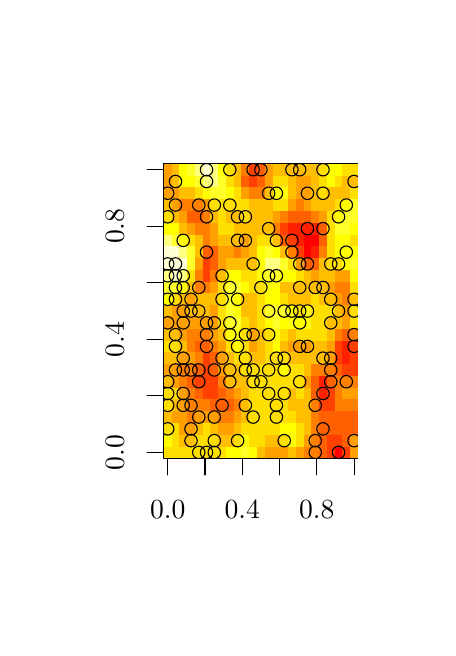
\begin{tikzpicture}[x=1pt,y=1pt]
\definecolor{fillColor}{RGB}{255,255,255}
\path[use as bounding box,fill=fillColor,fill opacity=0.00] (0,0) rectangle (144.54,216.81);
\begin{scope}
\path[clip] (  0.00,  0.00) rectangle (144.54,216.81);
\definecolor{drawColor}{RGB}{0,0,0}

\path[draw=drawColor,line width= 0.4pt,line join=round,line cap=round] ( 50.60, 61.20) -- (117.94, 61.20);

\path[draw=drawColor,line width= 0.4pt,line join=round,line cap=round] ( 50.60, 61.20) -- ( 50.60, 55.20);

\path[draw=drawColor,line width= 0.4pt,line join=round,line cap=round] ( 64.07, 61.20) -- ( 64.07, 55.20);

\path[draw=drawColor,line width= 0.4pt,line join=round,line cap=round] ( 77.54, 61.20) -- ( 77.54, 55.20);

\path[draw=drawColor,line width= 0.4pt,line join=round,line cap=round] ( 91.00, 61.20) -- ( 91.00, 55.20);

\path[draw=drawColor,line width= 0.4pt,line join=round,line cap=round] (104.47, 61.20) -- (104.47, 55.20);

\path[draw=drawColor,line width= 0.4pt,line join=round,line cap=round] (117.94, 61.20) -- (117.94, 55.20);

\node[text=drawColor,anchor=base,inner sep=0pt, outer sep=0pt, scale=  1.00] at ( 50.60, 39.60) {0.0};

\node[text=drawColor,anchor=base,inner sep=0pt, outer sep=0pt, scale=  1.00] at ( 77.54, 39.60) {0.4};

\node[text=drawColor,anchor=base,inner sep=0pt, outer sep=0pt, scale=  1.00] at (104.47, 39.60) {0.8};

\path[draw=drawColor,line width= 0.4pt,line join=round,line cap=round] ( 49.20, 63.33) -- ( 49.20,165.48);

\path[draw=drawColor,line width= 0.4pt,line join=round,line cap=round] ( 49.20, 63.33) -- ( 43.20, 63.33);

\path[draw=drawColor,line width= 0.4pt,line join=round,line cap=round] ( 49.20, 83.76) -- ( 43.20, 83.76);

\path[draw=drawColor,line width= 0.4pt,line join=round,line cap=round] ( 49.20,104.19) -- ( 43.20,104.19);

\path[draw=drawColor,line width= 0.4pt,line join=round,line cap=round] ( 49.20,124.62) -- ( 43.20,124.62);

\path[draw=drawColor,line width= 0.4pt,line join=round,line cap=round] ( 49.20,145.05) -- ( 43.20,145.05);

\path[draw=drawColor,line width= 0.4pt,line join=round,line cap=round] ( 49.20,165.48) -- ( 43.20,165.48);

\node[text=drawColor,rotate= 90.00,anchor=base,inner sep=0pt, outer sep=0pt, scale=  1.00] at ( 34.80, 63.33) {0.0};

\node[text=drawColor,rotate= 90.00,anchor=base,inner sep=0pt, outer sep=0pt, scale=  1.00] at ( 34.80,104.19) {0.4};

\node[text=drawColor,rotate= 90.00,anchor=base,inner sep=0pt, outer sep=0pt, scale=  1.00] at ( 34.80,145.05) {0.8};

\path[draw=drawColor,line width= 0.4pt,line join=round,line cap=round] ( 49.20, 61.20) --
	(119.34, 61.20) --
	(119.34,167.61) --
	( 49.20,167.61) --
	( 49.20, 61.20);
\end{scope}
\begin{scope}
\path[clip] ( 49.20, 61.20) rectangle (119.34,167.61);
\definecolor{fillColor}{RGB}{255,223,0}

\path[fill=fillColor] ( 49.20, 61.20) rectangle ( 52.01, 65.46);
\definecolor{fillColor}{RGB}{255,255,0}

\path[fill=fillColor] ( 49.20, 65.46) rectangle ( 52.01, 69.71);
\definecolor{fillColor}{RGB}{255,223,0}

\path[fill=fillColor] ( 49.20, 69.71) rectangle ( 52.01, 73.97);
\definecolor{fillColor}{RGB}{255,191,0}

\path[fill=fillColor] ( 49.20, 73.97) rectangle ( 52.01, 78.23);
\definecolor{fillColor}{RGB}{255,223,0}

\path[fill=fillColor] ( 49.20, 78.23) rectangle ( 52.01, 82.48);

\path[fill=fillColor] ( 49.20, 82.48) rectangle ( 52.01, 86.74);
\definecolor{fillColor}{RGB}{255,191,0}

\path[fill=fillColor] ( 49.20, 86.74) rectangle ( 52.01, 90.99);
\definecolor{fillColor}{RGB}{255,159,0}

\path[fill=fillColor] ( 49.20, 90.99) rectangle ( 52.01, 95.25);
\definecolor{fillColor}{RGB}{255,191,0}

\path[fill=fillColor] ( 49.20, 95.25) rectangle ( 52.01, 99.51);
\definecolor{fillColor}{RGB}{255,223,0}

\path[fill=fillColor] ( 49.20, 99.51) rectangle ( 52.01,103.76);
\definecolor{fillColor}{RGB}{255,191,0}

\path[fill=fillColor] ( 49.20,103.76) rectangle ( 52.01,108.02);
\definecolor{fillColor}{RGB}{255,159,0}

\path[fill=fillColor] ( 49.20,108.02) rectangle ( 52.01,112.28);
\definecolor{fillColor}{RGB}{255,191,0}

\path[fill=fillColor] ( 49.20,112.28) rectangle ( 52.01,116.53);
\definecolor{fillColor}{RGB}{255,255,0}

\path[fill=fillColor] ( 49.20,116.53) rectangle ( 52.01,120.79);
\definecolor{fillColor}{RGB}{255,255,42}

\path[fill=fillColor] ( 49.20,120.79) rectangle ( 52.01,125.05);
\definecolor{fillColor}{RGB}{255,255,128}

\path[fill=fillColor] ( 49.20,125.05) rectangle ( 52.01,129.30);
\definecolor{fillColor}{RGB}{255,255,213}

\path[fill=fillColor] ( 49.20,129.30) rectangle ( 52.01,133.56);

\path[fill=fillColor] ( 49.20,133.56) rectangle ( 52.01,137.82);
\definecolor{fillColor}{RGB}{255,255,128}

\path[fill=fillColor] ( 49.20,137.82) rectangle ( 52.01,142.07);
\definecolor{fillColor}{RGB}{255,255,0}

\path[fill=fillColor] ( 49.20,142.07) rectangle ( 52.01,146.33);
\definecolor{fillColor}{RGB}{255,223,0}

\path[fill=fillColor] ( 49.20,146.33) rectangle ( 52.01,150.58);
\definecolor{fillColor}{RGB}{255,191,0}

\path[fill=fillColor] ( 49.20,150.58) rectangle ( 52.01,154.84);
\definecolor{fillColor}{RGB}{255,159,0}

\path[fill=fillColor] ( 49.20,154.84) rectangle ( 52.01,159.10);

\path[fill=fillColor] ( 49.20,159.10) rectangle ( 52.01,163.35);

\path[fill=fillColor] ( 49.20,163.35) rectangle ( 52.01,167.61);
\definecolor{fillColor}{RGB}{255,223,0}

\path[fill=fillColor] ( 52.01, 61.20) rectangle ( 54.81, 65.46);

\path[fill=fillColor] ( 52.01, 65.46) rectangle ( 54.81, 69.71);

\path[fill=fillColor] ( 52.01, 69.71) rectangle ( 54.81, 73.97);
\definecolor{fillColor}{RGB}{255,159,0}

\path[fill=fillColor] ( 52.01, 73.97) rectangle ( 54.81, 78.23);
\definecolor{fillColor}{RGB}{255,191,0}

\path[fill=fillColor] ( 52.01, 78.23) rectangle ( 54.81, 82.48);
\definecolor{fillColor}{RGB}{255,223,0}

\path[fill=fillColor] ( 52.01, 82.48) rectangle ( 54.81, 86.74);
\definecolor{fillColor}{RGB}{255,159,0}

\path[fill=fillColor] ( 52.01, 86.74) rectangle ( 54.81, 90.99);

\path[fill=fillColor] ( 52.01, 90.99) rectangle ( 54.81, 95.25);
\definecolor{fillColor}{RGB}{255,191,0}

\path[fill=fillColor] ( 52.01, 95.25) rectangle ( 54.81, 99.51);
\definecolor{fillColor}{RGB}{255,223,0}

\path[fill=fillColor] ( 52.01, 99.51) rectangle ( 54.81,103.76);
\definecolor{fillColor}{RGB}{255,191,0}

\path[fill=fillColor] ( 52.01,103.76) rectangle ( 54.81,108.02);
\definecolor{fillColor}{RGB}{255,159,0}

\path[fill=fillColor] ( 52.01,108.02) rectangle ( 54.81,112.28);

\path[fill=fillColor] ( 52.01,112.28) rectangle ( 54.81,116.53);
\definecolor{fillColor}{RGB}{255,223,0}

\path[fill=fillColor] ( 52.01,116.53) rectangle ( 54.81,120.79);
\definecolor{fillColor}{RGB}{255,255,42}

\path[fill=fillColor] ( 52.01,120.79) rectangle ( 54.81,125.05);
\definecolor{fillColor}{RGB}{255,255,213}

\path[fill=fillColor] ( 52.01,125.05) rectangle ( 54.81,129.30);

\path[fill=fillColor] ( 52.01,129.30) rectangle ( 54.81,133.56);

\path[fill=fillColor] ( 52.01,133.56) rectangle ( 54.81,137.82);
\definecolor{fillColor}{RGB}{255,255,42}

\path[fill=fillColor] ( 52.01,137.82) rectangle ( 54.81,142.07);
\definecolor{fillColor}{RGB}{255,255,0}

\path[fill=fillColor] ( 52.01,142.07) rectangle ( 54.81,146.33);
\definecolor{fillColor}{RGB}{255,191,0}

\path[fill=fillColor] ( 52.01,146.33) rectangle ( 54.81,150.58);
\definecolor{fillColor}{RGB}{255,159,0}

\path[fill=fillColor] ( 52.01,150.58) rectangle ( 54.81,154.84);

\path[fill=fillColor] ( 52.01,154.84) rectangle ( 54.81,159.10);
\definecolor{fillColor}{RGB}{255,191,0}

\path[fill=fillColor] ( 52.01,159.10) rectangle ( 54.81,163.35);

\path[fill=fillColor] ( 52.01,163.35) rectangle ( 54.81,167.61);
\definecolor{fillColor}{RGB}{255,223,0}

\path[fill=fillColor] ( 54.81, 61.20) rectangle ( 57.62, 65.46);
\definecolor{fillColor}{RGB}{255,191,0}

\path[fill=fillColor] ( 54.81, 65.46) rectangle ( 57.62, 69.71);
\definecolor{fillColor}{RGB}{255,159,0}

\path[fill=fillColor] ( 54.81, 69.71) rectangle ( 57.62, 73.97);

\path[fill=fillColor] ( 54.81, 73.97) rectangle ( 57.62, 78.23);

\path[fill=fillColor] ( 54.81, 78.23) rectangle ( 57.62, 82.48);

\path[fill=fillColor] ( 54.81, 82.48) rectangle ( 57.62, 86.74);
\definecolor{fillColor}{RGB}{255,128,0}

\path[fill=fillColor] ( 54.81, 86.74) rectangle ( 57.62, 90.99);

\path[fill=fillColor] ( 54.81, 90.99) rectangle ( 57.62, 95.25);
\definecolor{fillColor}{RGB}{255,159,0}

\path[fill=fillColor] ( 54.81, 95.25) rectangle ( 57.62, 99.51);
\definecolor{fillColor}{RGB}{255,191,0}

\path[fill=fillColor] ( 54.81, 99.51) rectangle ( 57.62,103.76);
\definecolor{fillColor}{RGB}{255,159,0}

\path[fill=fillColor] ( 54.81,103.76) rectangle ( 57.62,108.02);

\path[fill=fillColor] ( 54.81,108.02) rectangle ( 57.62,112.28);

\path[fill=fillColor] ( 54.81,112.28) rectangle ( 57.62,116.53);
\definecolor{fillColor}{RGB}{255,191,0}

\path[fill=fillColor] ( 54.81,116.53) rectangle ( 57.62,120.79);
\definecolor{fillColor}{RGB}{255,255,0}

\path[fill=fillColor] ( 54.81,120.79) rectangle ( 57.62,125.05);
\definecolor{fillColor}{RGB}{255,255,128}

\path[fill=fillColor] ( 54.81,125.05) rectangle ( 57.62,129.30);
\definecolor{fillColor}{RGB}{255,255,213}

\path[fill=fillColor] ( 54.81,129.30) rectangle ( 57.62,133.56);
\definecolor{fillColor}{RGB}{255,255,128}

\path[fill=fillColor] ( 54.81,133.56) rectangle ( 57.62,137.82);
\definecolor{fillColor}{RGB}{255,255,0}

\path[fill=fillColor] ( 54.81,137.82) rectangle ( 57.62,142.07);
\definecolor{fillColor}{RGB}{255,191,0}

\path[fill=fillColor] ( 54.81,142.07) rectangle ( 57.62,146.33);
\definecolor{fillColor}{RGB}{255,159,0}

\path[fill=fillColor] ( 54.81,146.33) rectangle ( 57.62,150.58);
\definecolor{fillColor}{RGB}{255,128,0}

\path[fill=fillColor] ( 54.81,150.58) rectangle ( 57.62,154.84);
\definecolor{fillColor}{RGB}{255,191,0}

\path[fill=fillColor] ( 54.81,154.84) rectangle ( 57.62,159.10);
\definecolor{fillColor}{RGB}{255,255,0}

\path[fill=fillColor] ( 54.81,159.10) rectangle ( 57.62,163.35);

\path[fill=fillColor] ( 54.81,163.35) rectangle ( 57.62,167.61);
\definecolor{fillColor}{RGB}{255,223,0}

\path[fill=fillColor] ( 57.62, 61.20) rectangle ( 60.42, 65.46);
\definecolor{fillColor}{RGB}{255,191,0}

\path[fill=fillColor] ( 57.62, 65.46) rectangle ( 60.42, 69.71);
\definecolor{fillColor}{RGB}{255,159,0}

\path[fill=fillColor] ( 57.62, 69.71) rectangle ( 60.42, 73.97);
\definecolor{fillColor}{RGB}{255,128,0}

\path[fill=fillColor] ( 57.62, 73.97) rectangle ( 60.42, 78.23);

\path[fill=fillColor] ( 57.62, 78.23) rectangle ( 60.42, 82.48);

\path[fill=fillColor] ( 57.62, 82.48) rectangle ( 60.42, 86.74);
\definecolor{fillColor}{RGB}{255,96,0}

\path[fill=fillColor] ( 57.62, 86.74) rectangle ( 60.42, 90.99);
\definecolor{fillColor}{RGB}{255,128,0}

\path[fill=fillColor] ( 57.62, 90.99) rectangle ( 60.42, 95.25);
\definecolor{fillColor}{RGB}{255,159,0}

\path[fill=fillColor] ( 57.62, 95.25) rectangle ( 60.42, 99.51);
\definecolor{fillColor}{RGB}{255,128,0}

\path[fill=fillColor] ( 57.62, 99.51) rectangle ( 60.42,103.76);

\path[fill=fillColor] ( 57.62,103.76) rectangle ( 60.42,108.02);
\definecolor{fillColor}{RGB}{255,159,0}

\path[fill=fillColor] ( 57.62,108.02) rectangle ( 60.42,112.28);
\definecolor{fillColor}{RGB}{255,191,0}

\path[fill=fillColor] ( 57.62,112.28) rectangle ( 60.42,116.53);
\definecolor{fillColor}{RGB}{255,159,0}

\path[fill=fillColor] ( 57.62,116.53) rectangle ( 60.42,120.79);
\definecolor{fillColor}{RGB}{255,191,0}

\path[fill=fillColor] ( 57.62,120.79) rectangle ( 60.42,125.05);
\definecolor{fillColor}{RGB}{255,223,0}

\path[fill=fillColor] ( 57.62,125.05) rectangle ( 60.42,129.30);
\definecolor{fillColor}{RGB}{255,255,42}

\path[fill=fillColor] ( 57.62,129.30) rectangle ( 60.42,133.56);

\path[fill=fillColor] ( 57.62,133.56) rectangle ( 60.42,137.82);
\definecolor{fillColor}{RGB}{255,223,0}

\path[fill=fillColor] ( 57.62,137.82) rectangle ( 60.42,142.07);
\definecolor{fillColor}{RGB}{255,159,0}

\path[fill=fillColor] ( 57.62,142.07) rectangle ( 60.42,146.33);
\definecolor{fillColor}{RGB}{255,96,0}

\path[fill=fillColor] ( 57.62,146.33) rectangle ( 60.42,150.58);
\definecolor{fillColor}{RGB}{255,128,0}

\path[fill=fillColor] ( 57.62,150.58) rectangle ( 60.42,154.84);
\definecolor{fillColor}{RGB}{255,191,0}

\path[fill=fillColor] ( 57.62,154.84) rectangle ( 60.42,159.10);
\definecolor{fillColor}{RGB}{255,255,0}

\path[fill=fillColor] ( 57.62,159.10) rectangle ( 60.42,163.35);
\definecolor{fillColor}{RGB}{255,255,42}

\path[fill=fillColor] ( 57.62,163.35) rectangle ( 60.42,167.61);
\definecolor{fillColor}{RGB}{255,223,0}

\path[fill=fillColor] ( 60.42, 61.20) rectangle ( 63.23, 65.46);

\path[fill=fillColor] ( 60.42, 65.46) rectangle ( 63.23, 69.71);
\definecolor{fillColor}{RGB}{255,191,0}

\path[fill=fillColor] ( 60.42, 69.71) rectangle ( 63.23, 73.97);
\definecolor{fillColor}{RGB}{255,159,0}

\path[fill=fillColor] ( 60.42, 73.97) rectangle ( 63.23, 78.23);
\definecolor{fillColor}{RGB}{255,128,0}

\path[fill=fillColor] ( 60.42, 78.23) rectangle ( 63.23, 82.48);
\definecolor{fillColor}{RGB}{255,96,0}

\path[fill=fillColor] ( 60.42, 82.48) rectangle ( 63.23, 86.74);
\definecolor{fillColor}{RGB}{255,64,0}

\path[fill=fillColor] ( 60.42, 86.74) rectangle ( 63.23, 90.99);
\definecolor{fillColor}{RGB}{255,96,0}

\path[fill=fillColor] ( 60.42, 90.99) rectangle ( 63.23, 95.25);
\definecolor{fillColor}{RGB}{255,128,0}

\path[fill=fillColor] ( 60.42, 95.25) rectangle ( 63.23, 99.51);
\definecolor{fillColor}{RGB}{255,96,0}

\path[fill=fillColor] ( 60.42, 99.51) rectangle ( 63.23,103.76);
\definecolor{fillColor}{RGB}{255,128,0}

\path[fill=fillColor] ( 60.42,103.76) rectangle ( 63.23,108.02);
\definecolor{fillColor}{RGB}{255,159,0}

\path[fill=fillColor] ( 60.42,108.02) rectangle ( 63.23,112.28);
\definecolor{fillColor}{RGB}{255,191,0}

\path[fill=fillColor] ( 60.42,112.28) rectangle ( 63.23,116.53);

\path[fill=fillColor] ( 60.42,116.53) rectangle ( 63.23,120.79);
\definecolor{fillColor}{RGB}{255,128,0}

\path[fill=fillColor] ( 60.42,120.79) rectangle ( 63.23,125.05);

\path[fill=fillColor] ( 60.42,125.05) rectangle ( 63.23,129.30);
\definecolor{fillColor}{RGB}{255,159,0}

\path[fill=fillColor] ( 60.42,129.30) rectangle ( 63.23,133.56);
\definecolor{fillColor}{RGB}{255,191,0}

\path[fill=fillColor] ( 60.42,133.56) rectangle ( 63.23,137.82);

\path[fill=fillColor] ( 60.42,137.82) rectangle ( 63.23,142.07);
\definecolor{fillColor}{RGB}{255,128,0}

\path[fill=fillColor] ( 60.42,142.07) rectangle ( 63.23,146.33);
\definecolor{fillColor}{RGB}{255,96,0}

\path[fill=fillColor] ( 60.42,146.33) rectangle ( 63.23,150.58);
\definecolor{fillColor}{RGB}{255,128,0}

\path[fill=fillColor] ( 60.42,150.58) rectangle ( 63.23,154.84);
\definecolor{fillColor}{RGB}{255,223,0}

\path[fill=fillColor] ( 60.42,154.84) rectangle ( 63.23,159.10);
\definecolor{fillColor}{RGB}{255,255,42}

\path[fill=fillColor] ( 60.42,159.10) rectangle ( 63.23,163.35);
\definecolor{fillColor}{RGB}{255,255,128}

\path[fill=fillColor] ( 60.42,163.35) rectangle ( 63.23,167.61);
\definecolor{fillColor}{RGB}{255,223,0}

\path[fill=fillColor] ( 63.23, 61.20) rectangle ( 66.03, 65.46);

\path[fill=fillColor] ( 63.23, 65.46) rectangle ( 66.03, 69.71);

\path[fill=fillColor] ( 63.23, 69.71) rectangle ( 66.03, 73.97);
\definecolor{fillColor}{RGB}{255,159,0}

\path[fill=fillColor] ( 63.23, 73.97) rectangle ( 66.03, 78.23);
\definecolor{fillColor}{RGB}{255,128,0}

\path[fill=fillColor] ( 63.23, 78.23) rectangle ( 66.03, 82.48);
\definecolor{fillColor}{RGB}{255,64,0}

\path[fill=fillColor] ( 63.23, 82.48) rectangle ( 66.03, 86.74);

\path[fill=fillColor] ( 63.23, 86.74) rectangle ( 66.03, 90.99);

\path[fill=fillColor] ( 63.23, 90.99) rectangle ( 66.03, 95.25);

\path[fill=fillColor] ( 63.23, 95.25) rectangle ( 66.03, 99.51);
\definecolor{fillColor}{RGB}{255,96,0}

\path[fill=fillColor] ( 63.23, 99.51) rectangle ( 66.03,103.76);
\definecolor{fillColor}{RGB}{255,128,0}

\path[fill=fillColor] ( 63.23,103.76) rectangle ( 66.03,108.02);
\definecolor{fillColor}{RGB}{255,159,0}

\path[fill=fillColor] ( 63.23,108.02) rectangle ( 66.03,112.28);
\definecolor{fillColor}{RGB}{255,191,0}

\path[fill=fillColor] ( 63.23,112.28) rectangle ( 66.03,116.53);

\path[fill=fillColor] ( 63.23,116.53) rectangle ( 66.03,120.79);
\definecolor{fillColor}{RGB}{255,128,0}

\path[fill=fillColor] ( 63.23,120.79) rectangle ( 66.03,125.05);
\definecolor{fillColor}{RGB}{255,64,0}

\path[fill=fillColor] ( 63.23,125.05) rectangle ( 66.03,129.30);

\path[fill=fillColor] ( 63.23,129.30) rectangle ( 66.03,133.56);
\definecolor{fillColor}{RGB}{255,96,0}

\path[fill=fillColor] ( 63.23,133.56) rectangle ( 66.03,137.82);
\definecolor{fillColor}{RGB}{255,128,0}

\path[fill=fillColor] ( 63.23,137.82) rectangle ( 66.03,142.07);

\path[fill=fillColor] ( 63.23,142.07) rectangle ( 66.03,146.33);

\path[fill=fillColor] ( 63.23,146.33) rectangle ( 66.03,150.58);
\definecolor{fillColor}{RGB}{255,159,0}

\path[fill=fillColor] ( 63.23,150.58) rectangle ( 66.03,154.84);
\definecolor{fillColor}{RGB}{255,255,0}

\path[fill=fillColor] ( 63.23,154.84) rectangle ( 66.03,159.10);
\definecolor{fillColor}{RGB}{255,255,128}

\path[fill=fillColor] ( 63.23,159.10) rectangle ( 66.03,163.35);
\definecolor{fillColor}{RGB}{255,255,213}

\path[fill=fillColor] ( 63.23,163.35) rectangle ( 66.03,167.61);
\definecolor{fillColor}{RGB}{255,223,0}

\path[fill=fillColor] ( 66.03, 61.20) rectangle ( 68.84, 65.46);

\path[fill=fillColor] ( 66.03, 65.46) rectangle ( 68.84, 69.71);
\definecolor{fillColor}{RGB}{255,191,0}

\path[fill=fillColor] ( 66.03, 69.71) rectangle ( 68.84, 73.97);
\definecolor{fillColor}{RGB}{255,159,0}

\path[fill=fillColor] ( 66.03, 73.97) rectangle ( 68.84, 78.23);
\definecolor{fillColor}{RGB}{255,96,0}

\path[fill=fillColor] ( 66.03, 78.23) rectangle ( 68.84, 82.48);
\definecolor{fillColor}{RGB}{255,64,0}

\path[fill=fillColor] ( 66.03, 82.48) rectangle ( 68.84, 86.74);

\path[fill=fillColor] ( 66.03, 86.74) rectangle ( 68.84, 90.99);
\definecolor{fillColor}{RGB}{255,96,0}

\path[fill=fillColor] ( 66.03, 90.99) rectangle ( 68.84, 95.25);

\path[fill=fillColor] ( 66.03, 95.25) rectangle ( 68.84, 99.51);
\definecolor{fillColor}{RGB}{255,128,0}

\path[fill=fillColor] ( 66.03, 99.51) rectangle ( 68.84,103.76);
\definecolor{fillColor}{RGB}{255,159,0}

\path[fill=fillColor] ( 66.03,103.76) rectangle ( 68.84,108.02);

\path[fill=fillColor] ( 66.03,108.02) rectangle ( 68.84,112.28);

\path[fill=fillColor] ( 66.03,112.28) rectangle ( 68.84,116.53);
\definecolor{fillColor}{RGB}{255,191,0}

\path[fill=fillColor] ( 66.03,116.53) rectangle ( 68.84,120.79);
\definecolor{fillColor}{RGB}{255,159,0}

\path[fill=fillColor] ( 66.03,120.79) rectangle ( 68.84,125.05);
\definecolor{fillColor}{RGB}{255,128,0}

\path[fill=fillColor] ( 66.03,125.05) rectangle ( 68.84,129.30);
\definecolor{fillColor}{RGB}{255,96,0}

\path[fill=fillColor] ( 66.03,129.30) rectangle ( 68.84,133.56);

\path[fill=fillColor] ( 66.03,133.56) rectangle ( 68.84,137.82);
\definecolor{fillColor}{RGB}{255,159,0}

\path[fill=fillColor] ( 66.03,137.82) rectangle ( 68.84,142.07);

\path[fill=fillColor] ( 66.03,142.07) rectangle ( 68.84,146.33);
\definecolor{fillColor}{RGB}{255,191,0}

\path[fill=fillColor] ( 66.03,146.33) rectangle ( 68.84,150.58);
\definecolor{fillColor}{RGB}{255,223,0}

\path[fill=fillColor] ( 66.03,150.58) rectangle ( 68.84,154.84);
\definecolor{fillColor}{RGB}{255,255,42}

\path[fill=fillColor] ( 66.03,154.84) rectangle ( 68.84,159.10);
\definecolor{fillColor}{RGB}{255,255,128}

\path[fill=fillColor] ( 66.03,159.10) rectangle ( 68.84,163.35);

\path[fill=fillColor] ( 66.03,163.35) rectangle ( 68.84,167.61);
\definecolor{fillColor}{RGB}{255,223,0}

\path[fill=fillColor] ( 68.84, 61.20) rectangle ( 71.64, 65.46);
\definecolor{fillColor}{RGB}{255,191,0}

\path[fill=fillColor] ( 68.84, 65.46) rectangle ( 71.64, 69.71);
\definecolor{fillColor}{RGB}{255,159,0}

\path[fill=fillColor] ( 68.84, 69.71) rectangle ( 71.64, 73.97);
\definecolor{fillColor}{RGB}{255,128,0}

\path[fill=fillColor] ( 68.84, 73.97) rectangle ( 71.64, 78.23);
\definecolor{fillColor}{RGB}{255,96,0}

\path[fill=fillColor] ( 68.84, 78.23) rectangle ( 71.64, 82.48);

\path[fill=fillColor] ( 68.84, 82.48) rectangle ( 71.64, 86.74);
\definecolor{fillColor}{RGB}{255,128,0}

\path[fill=fillColor] ( 68.84, 86.74) rectangle ( 71.64, 90.99);
\definecolor{fillColor}{RGB}{255,159,0}

\path[fill=fillColor] ( 68.84, 90.99) rectangle ( 71.64, 95.25);

\path[fill=fillColor] ( 68.84, 95.25) rectangle ( 71.64, 99.51);

\path[fill=fillColor] ( 68.84, 99.51) rectangle ( 71.64,103.76);
\definecolor{fillColor}{RGB}{255,191,0}

\path[fill=fillColor] ( 68.84,103.76) rectangle ( 71.64,108.02);
\definecolor{fillColor}{RGB}{255,223,0}

\path[fill=fillColor] ( 68.84,108.02) rectangle ( 71.64,112.28);

\path[fill=fillColor] ( 68.84,112.28) rectangle ( 71.64,116.53);

\path[fill=fillColor] ( 68.84,116.53) rectangle ( 71.64,120.79);

\path[fill=fillColor] ( 68.84,120.79) rectangle ( 71.64,125.05);
\definecolor{fillColor}{RGB}{255,191,0}

\path[fill=fillColor] ( 68.84,125.05) rectangle ( 71.64,129.30);
\definecolor{fillColor}{RGB}{255,159,0}

\path[fill=fillColor] ( 68.84,129.30) rectangle ( 71.64,133.56);

\path[fill=fillColor] ( 68.84,133.56) rectangle ( 71.64,137.82);
\definecolor{fillColor}{RGB}{255,191,0}

\path[fill=fillColor] ( 68.84,137.82) rectangle ( 71.64,142.07);
\definecolor{fillColor}{RGB}{255,223,0}

\path[fill=fillColor] ( 68.84,142.07) rectangle ( 71.64,146.33);

\path[fill=fillColor] ( 68.84,146.33) rectangle ( 71.64,150.58);

\path[fill=fillColor] ( 68.84,150.58) rectangle ( 71.64,154.84);
\definecolor{fillColor}{RGB}{255,255,42}

\path[fill=fillColor] ( 68.84,154.84) rectangle ( 71.64,159.10);

\path[fill=fillColor] ( 68.84,159.10) rectangle ( 71.64,163.35);
\definecolor{fillColor}{RGB}{255,255,0}

\path[fill=fillColor] ( 68.84,163.35) rectangle ( 71.64,167.61);

\path[fill=fillColor] ( 71.64, 61.20) rectangle ( 74.45, 65.46);
\definecolor{fillColor}{RGB}{255,191,0}

\path[fill=fillColor] ( 71.64, 65.46) rectangle ( 74.45, 69.71);
\definecolor{fillColor}{RGB}{255,159,0}

\path[fill=fillColor] ( 71.64, 69.71) rectangle ( 74.45, 73.97);
\definecolor{fillColor}{RGB}{255,128,0}

\path[fill=fillColor] ( 71.64, 73.97) rectangle ( 74.45, 78.23);
\definecolor{fillColor}{RGB}{255,96,0}

\path[fill=fillColor] ( 71.64, 78.23) rectangle ( 74.45, 82.48);
\definecolor{fillColor}{RGB}{255,128,0}

\path[fill=fillColor] ( 71.64, 82.48) rectangle ( 74.45, 86.74);
\definecolor{fillColor}{RGB}{255,191,0}

\path[fill=fillColor] ( 71.64, 86.74) rectangle ( 74.45, 90.99);

\path[fill=fillColor] ( 71.64, 90.99) rectangle ( 74.45, 95.25);

\path[fill=fillColor] ( 71.64, 95.25) rectangle ( 74.45, 99.51);
\definecolor{fillColor}{RGB}{255,223,0}

\path[fill=fillColor] ( 71.64, 99.51) rectangle ( 74.45,103.76);
\definecolor{fillColor}{RGB}{255,255,0}

\path[fill=fillColor] ( 71.64,103.76) rectangle ( 74.45,108.02);
\definecolor{fillColor}{RGB}{255,255,42}

\path[fill=fillColor] ( 71.64,108.02) rectangle ( 74.45,112.28);

\path[fill=fillColor] ( 71.64,112.28) rectangle ( 74.45,116.53);

\path[fill=fillColor] ( 71.64,116.53) rectangle ( 74.45,120.79);

\path[fill=fillColor] ( 71.64,120.79) rectangle ( 74.45,125.05);
\definecolor{fillColor}{RGB}{255,255,0}

\path[fill=fillColor] ( 71.64,125.05) rectangle ( 74.45,129.30);
\definecolor{fillColor}{RGB}{255,191,0}

\path[fill=fillColor] ( 71.64,129.30) rectangle ( 74.45,133.56);
\definecolor{fillColor}{RGB}{255,159,0}

\path[fill=fillColor] ( 71.64,133.56) rectangle ( 74.45,137.82);
\definecolor{fillColor}{RGB}{255,191,0}

\path[fill=fillColor] ( 71.64,137.82) rectangle ( 74.45,142.07);
\definecolor{fillColor}{RGB}{255,223,0}

\path[fill=fillColor] ( 71.64,142.07) rectangle ( 74.45,146.33);
\definecolor{fillColor}{RGB}{255,191,0}

\path[fill=fillColor] ( 71.64,146.33) rectangle ( 74.45,150.58);
\definecolor{fillColor}{RGB}{255,223,0}

\path[fill=fillColor] ( 71.64,150.58) rectangle ( 74.45,154.84);
\definecolor{fillColor}{RGB}{255,255,0}

\path[fill=fillColor] ( 71.64,154.84) rectangle ( 74.45,159.10);
\definecolor{fillColor}{RGB}{255,223,0}

\path[fill=fillColor] ( 71.64,159.10) rectangle ( 74.45,163.35);

\path[fill=fillColor] ( 71.64,163.35) rectangle ( 74.45,167.61);
\definecolor{fillColor}{RGB}{255,255,0}

\path[fill=fillColor] ( 74.45, 61.20) rectangle ( 77.26, 65.46);
\definecolor{fillColor}{RGB}{255,223,0}

\path[fill=fillColor] ( 74.45, 65.46) rectangle ( 77.26, 69.71);
\definecolor{fillColor}{RGB}{255,191,0}

\path[fill=fillColor] ( 74.45, 69.71) rectangle ( 77.26, 73.97);
\definecolor{fillColor}{RGB}{255,159,0}

\path[fill=fillColor] ( 74.45, 73.97) rectangle ( 77.26, 78.23);
\definecolor{fillColor}{RGB}{255,128,0}

\path[fill=fillColor] ( 74.45, 78.23) rectangle ( 77.26, 82.48);
\definecolor{fillColor}{RGB}{255,159,0}

\path[fill=fillColor] ( 74.45, 82.48) rectangle ( 77.26, 86.74);
\definecolor{fillColor}{RGB}{255,191,0}

\path[fill=fillColor] ( 74.45, 86.74) rectangle ( 77.26, 90.99);

\path[fill=fillColor] ( 74.45, 90.99) rectangle ( 77.26, 95.25);
\definecolor{fillColor}{RGB}{255,223,0}

\path[fill=fillColor] ( 74.45, 95.25) rectangle ( 77.26, 99.51);
\definecolor{fillColor}{RGB}{255,255,0}

\path[fill=fillColor] ( 74.45, 99.51) rectangle ( 77.26,103.76);

\path[fill=fillColor] ( 74.45,103.76) rectangle ( 77.26,108.02);
\definecolor{fillColor}{RGB}{255,255,42}

\path[fill=fillColor] ( 74.45,108.02) rectangle ( 77.26,112.28);
\definecolor{fillColor}{RGB}{255,255,0}

\path[fill=fillColor] ( 74.45,112.28) rectangle ( 77.26,116.53);

\path[fill=fillColor] ( 74.45,116.53) rectangle ( 77.26,120.79);
\definecolor{fillColor}{RGB}{255,255,42}

\path[fill=fillColor] ( 74.45,120.79) rectangle ( 77.26,125.05);
\definecolor{fillColor}{RGB}{255,255,0}

\path[fill=fillColor] ( 74.45,125.05) rectangle ( 77.26,129.30);
\definecolor{fillColor}{RGB}{255,191,0}

\path[fill=fillColor] ( 74.45,129.30) rectangle ( 77.26,133.56);
\definecolor{fillColor}{RGB}{255,128,0}

\path[fill=fillColor] ( 74.45,133.56) rectangle ( 77.26,137.82);
\definecolor{fillColor}{RGB}{255,191,0}

\path[fill=fillColor] ( 74.45,137.82) rectangle ( 77.26,142.07);

\path[fill=fillColor] ( 74.45,142.07) rectangle ( 77.26,146.33);

\path[fill=fillColor] ( 74.45,146.33) rectangle ( 77.26,150.58);
\definecolor{fillColor}{RGB}{255,223,0}

\path[fill=fillColor] ( 74.45,150.58) rectangle ( 77.26,154.84);

\path[fill=fillColor] ( 74.45,154.84) rectangle ( 77.26,159.10);
\definecolor{fillColor}{RGB}{255,191,0}

\path[fill=fillColor] ( 74.45,159.10) rectangle ( 77.26,163.35);

\path[fill=fillColor] ( 74.45,163.35) rectangle ( 77.26,167.61);
\definecolor{fillColor}{RGB}{255,255,42}

\path[fill=fillColor] ( 77.26, 61.20) rectangle ( 80.06, 65.46);
\definecolor{fillColor}{RGB}{255,255,0}

\path[fill=fillColor] ( 77.26, 65.46) rectangle ( 80.06, 69.71);
\definecolor{fillColor}{RGB}{255,223,0}

\path[fill=fillColor] ( 77.26, 69.71) rectangle ( 80.06, 73.97);
\definecolor{fillColor}{RGB}{255,191,0}

\path[fill=fillColor] ( 77.26, 73.97) rectangle ( 80.06, 78.23);

\path[fill=fillColor] ( 77.26, 78.23) rectangle ( 80.06, 82.48);

\path[fill=fillColor] ( 77.26, 82.48) rectangle ( 80.06, 86.74);

\path[fill=fillColor] ( 77.26, 86.74) rectangle ( 80.06, 90.99);
\definecolor{fillColor}{RGB}{255,223,0}

\path[fill=fillColor] ( 77.26, 90.99) rectangle ( 80.06, 95.25);

\path[fill=fillColor] ( 77.26, 95.25) rectangle ( 80.06, 99.51);

\path[fill=fillColor] ( 77.26, 99.51) rectangle ( 80.06,103.76);

\path[fill=fillColor] ( 77.26,103.76) rectangle ( 80.06,108.02);

\path[fill=fillColor] ( 77.26,108.02) rectangle ( 80.06,112.28);
\definecolor{fillColor}{RGB}{255,191,0}

\path[fill=fillColor] ( 77.26,112.28) rectangle ( 80.06,116.53);

\path[fill=fillColor] ( 77.26,116.53) rectangle ( 80.06,120.79);
\definecolor{fillColor}{RGB}{255,255,0}

\path[fill=fillColor] ( 77.26,120.79) rectangle ( 80.06,125.05);
\definecolor{fillColor}{RGB}{255,223,0}

\path[fill=fillColor] ( 77.26,125.05) rectangle ( 80.06,129.30);
\definecolor{fillColor}{RGB}{255,191,0}

\path[fill=fillColor] ( 77.26,129.30) rectangle ( 80.06,133.56);
\definecolor{fillColor}{RGB}{255,159,0}

\path[fill=fillColor] ( 77.26,133.56) rectangle ( 80.06,137.82);

\path[fill=fillColor] ( 77.26,137.82) rectangle ( 80.06,142.07);
\definecolor{fillColor}{RGB}{255,191,0}

\path[fill=fillColor] ( 77.26,142.07) rectangle ( 80.06,146.33);
\definecolor{fillColor}{RGB}{255,223,0}

\path[fill=fillColor] ( 77.26,146.33) rectangle ( 80.06,150.58);

\path[fill=fillColor] ( 77.26,150.58) rectangle ( 80.06,154.84);
\definecolor{fillColor}{RGB}{255,159,0}

\path[fill=fillColor] ( 77.26,154.84) rectangle ( 80.06,159.10);
\definecolor{fillColor}{RGB}{255,96,0}

\path[fill=fillColor] ( 77.26,159.10) rectangle ( 80.06,163.35);
\definecolor{fillColor}{RGB}{255,128,0}

\path[fill=fillColor] ( 77.26,163.35) rectangle ( 80.06,167.61);
\definecolor{fillColor}{RGB}{255,255,0}

\path[fill=fillColor] ( 80.06, 61.20) rectangle ( 82.87, 65.46);
\definecolor{fillColor}{RGB}{255,223,0}

\path[fill=fillColor] ( 80.06, 65.46) rectangle ( 82.87, 69.71);

\path[fill=fillColor] ( 80.06, 69.71) rectangle ( 82.87, 73.97);

\path[fill=fillColor] ( 80.06, 73.97) rectangle ( 82.87, 78.23);

\path[fill=fillColor] ( 80.06, 78.23) rectangle ( 82.87, 82.48);

\path[fill=fillColor] ( 80.06, 82.48) rectangle ( 82.87, 86.74);

\path[fill=fillColor] ( 80.06, 86.74) rectangle ( 82.87, 90.99);

\path[fill=fillColor] ( 80.06, 90.99) rectangle ( 82.87, 95.25);
\definecolor{fillColor}{RGB}{255,191,0}

\path[fill=fillColor] ( 80.06, 95.25) rectangle ( 82.87, 99.51);
\definecolor{fillColor}{RGB}{255,159,0}

\path[fill=fillColor] ( 80.06, 99.51) rectangle ( 82.87,103.76);

\path[fill=fillColor] ( 80.06,103.76) rectangle ( 82.87,108.02);
\definecolor{fillColor}{RGB}{255,191,0}

\path[fill=fillColor] ( 80.06,108.02) rectangle ( 82.87,112.28);

\path[fill=fillColor] ( 80.06,112.28) rectangle ( 82.87,116.53);

\path[fill=fillColor] ( 80.06,116.53) rectangle ( 82.87,120.79);
\definecolor{fillColor}{RGB}{255,223,0}

\path[fill=fillColor] ( 80.06,120.79) rectangle ( 82.87,125.05);

\path[fill=fillColor] ( 80.06,125.05) rectangle ( 82.87,129.30);
\definecolor{fillColor}{RGB}{255,191,0}

\path[fill=fillColor] ( 80.06,129.30) rectangle ( 82.87,133.56);

\path[fill=fillColor] ( 80.06,133.56) rectangle ( 82.87,137.82);

\path[fill=fillColor] ( 80.06,137.82) rectangle ( 82.87,142.07);

\path[fill=fillColor] ( 80.06,142.07) rectangle ( 82.87,146.33);

\path[fill=fillColor] ( 80.06,146.33) rectangle ( 82.87,150.58);

\path[fill=fillColor] ( 80.06,150.58) rectangle ( 82.87,154.84);
\definecolor{fillColor}{RGB}{255,128,0}

\path[fill=fillColor] ( 80.06,154.84) rectangle ( 82.87,159.10);
\definecolor{fillColor}{RGB}{255,64,0}

\path[fill=fillColor] ( 80.06,159.10) rectangle ( 82.87,163.35);

\path[fill=fillColor] ( 80.06,163.35) rectangle ( 82.87,167.61);
\definecolor{fillColor}{RGB}{255,191,0}

\path[fill=fillColor] ( 82.87, 61.20) rectangle ( 85.67, 65.46);
\definecolor{fillColor}{RGB}{255,223,0}

\path[fill=fillColor] ( 82.87, 65.46) rectangle ( 85.67, 69.71);

\path[fill=fillColor] ( 82.87, 69.71) rectangle ( 85.67, 73.97);

\path[fill=fillColor] ( 82.87, 73.97) rectangle ( 85.67, 78.23);

\path[fill=fillColor] ( 82.87, 78.23) rectangle ( 85.67, 82.48);

\path[fill=fillColor] ( 82.87, 82.48) rectangle ( 85.67, 86.74);

\path[fill=fillColor] ( 82.87, 86.74) rectangle ( 85.67, 90.99);

\path[fill=fillColor] ( 82.87, 90.99) rectangle ( 85.67, 95.25);
\definecolor{fillColor}{RGB}{255,191,0}

\path[fill=fillColor] ( 82.87, 95.25) rectangle ( 85.67, 99.51);

\path[fill=fillColor] ( 82.87, 99.51) rectangle ( 85.67,103.76);

\path[fill=fillColor] ( 82.87,103.76) rectangle ( 85.67,108.02);
\definecolor{fillColor}{RGB}{255,223,0}

\path[fill=fillColor] ( 82.87,108.02) rectangle ( 85.67,112.28);

\path[fill=fillColor] ( 82.87,112.28) rectangle ( 85.67,116.53);

\path[fill=fillColor] ( 82.87,116.53) rectangle ( 85.67,120.79);

\path[fill=fillColor] ( 82.87,120.79) rectangle ( 85.67,125.05);
\definecolor{fillColor}{RGB}{255,255,0}

\path[fill=fillColor] ( 82.87,125.05) rectangle ( 85.67,129.30);

\path[fill=fillColor] ( 82.87,129.30) rectangle ( 85.67,133.56);

\path[fill=fillColor] ( 82.87,133.56) rectangle ( 85.67,137.82);
\definecolor{fillColor}{RGB}{255,223,0}

\path[fill=fillColor] ( 82.87,137.82) rectangle ( 85.67,142.07);
\definecolor{fillColor}{RGB}{255,191,0}

\path[fill=fillColor] ( 82.87,142.07) rectangle ( 85.67,146.33);

\path[fill=fillColor] ( 82.87,146.33) rectangle ( 85.67,150.58);

\path[fill=fillColor] ( 82.87,150.58) rectangle ( 85.67,154.84);
\definecolor{fillColor}{RGB}{255,128,0}

\path[fill=fillColor] ( 82.87,154.84) rectangle ( 85.67,159.10);
\definecolor{fillColor}{RGB}{255,96,0}

\path[fill=fillColor] ( 82.87,159.10) rectangle ( 85.67,163.35);

\path[fill=fillColor] ( 82.87,163.35) rectangle ( 85.67,167.61);
\definecolor{fillColor}{RGB}{255,159,0}

\path[fill=fillColor] ( 85.67, 61.20) rectangle ( 88.48, 65.46);
\definecolor{fillColor}{RGB}{255,191,0}

\path[fill=fillColor] ( 85.67, 65.46) rectangle ( 88.48, 69.71);
\definecolor{fillColor}{RGB}{255,223,0}

\path[fill=fillColor] ( 85.67, 69.71) rectangle ( 88.48, 73.97);

\path[fill=fillColor] ( 85.67, 73.97) rectangle ( 88.48, 78.23);

\path[fill=fillColor] ( 85.67, 78.23) rectangle ( 88.48, 82.48);

\path[fill=fillColor] ( 85.67, 82.48) rectangle ( 88.48, 86.74);

\path[fill=fillColor] ( 85.67, 86.74) rectangle ( 88.48, 90.99);

\path[fill=fillColor] ( 85.67, 90.99) rectangle ( 88.48, 95.25);

\path[fill=fillColor] ( 85.67, 95.25) rectangle ( 88.48, 99.51);

\path[fill=fillColor] ( 85.67, 99.51) rectangle ( 88.48,103.76);

\path[fill=fillColor] ( 85.67,103.76) rectangle ( 88.48,108.02);
\definecolor{fillColor}{RGB}{255,255,0}

\path[fill=fillColor] ( 85.67,108.02) rectangle ( 88.48,112.28);
\definecolor{fillColor}{RGB}{255,255,42}

\path[fill=fillColor] ( 85.67,112.28) rectangle ( 88.48,116.53);
\definecolor{fillColor}{RGB}{255,255,0}

\path[fill=fillColor] ( 85.67,116.53) rectangle ( 88.48,120.79);

\path[fill=fillColor] ( 85.67,120.79) rectangle ( 88.48,125.05);
\definecolor{fillColor}{RGB}{255,255,42}

\path[fill=fillColor] ( 85.67,125.05) rectangle ( 88.48,129.30);
\definecolor{fillColor}{RGB}{255,255,128}

\path[fill=fillColor] ( 85.67,129.30) rectangle ( 88.48,133.56);
\definecolor{fillColor}{RGB}{255,255,42}

\path[fill=fillColor] ( 85.67,133.56) rectangle ( 88.48,137.82);
\definecolor{fillColor}{RGB}{255,223,0}

\path[fill=fillColor] ( 85.67,137.82) rectangle ( 88.48,142.07);
\definecolor{fillColor}{RGB}{255,191,0}

\path[fill=fillColor] ( 85.67,142.07) rectangle ( 88.48,146.33);

\path[fill=fillColor] ( 85.67,146.33) rectangle ( 88.48,150.58);

\path[fill=fillColor] ( 85.67,150.58) rectangle ( 88.48,154.84);

\path[fill=fillColor] ( 85.67,154.84) rectangle ( 88.48,159.10);
\definecolor{fillColor}{RGB}{255,159,0}

\path[fill=fillColor] ( 85.67,159.10) rectangle ( 88.48,163.35);

\path[fill=fillColor] ( 85.67,163.35) rectangle ( 88.48,167.61);

\path[fill=fillColor] ( 88.48, 61.20) rectangle ( 91.28, 65.46);
\definecolor{fillColor}{RGB}{255,191,0}

\path[fill=fillColor] ( 88.48, 65.46) rectangle ( 91.28, 69.71);
\definecolor{fillColor}{RGB}{255,223,0}

\path[fill=fillColor] ( 88.48, 69.71) rectangle ( 91.28, 73.97);

\path[fill=fillColor] ( 88.48, 73.97) rectangle ( 91.28, 78.23);

\path[fill=fillColor] ( 88.48, 78.23) rectangle ( 91.28, 82.48);

\path[fill=fillColor] ( 88.48, 82.48) rectangle ( 91.28, 86.74);

\path[fill=fillColor] ( 88.48, 86.74) rectangle ( 91.28, 90.99);

\path[fill=fillColor] ( 88.48, 90.99) rectangle ( 91.28, 95.25);

\path[fill=fillColor] ( 88.48, 95.25) rectangle ( 91.28, 99.51);
\definecolor{fillColor}{RGB}{255,255,0}

\path[fill=fillColor] ( 88.48, 99.51) rectangle ( 91.28,103.76);

\path[fill=fillColor] ( 88.48,103.76) rectangle ( 91.28,108.02);
\definecolor{fillColor}{RGB}{255,255,42}

\path[fill=fillColor] ( 88.48,108.02) rectangle ( 91.28,112.28);

\path[fill=fillColor] ( 88.48,112.28) rectangle ( 91.28,116.53);
\definecolor{fillColor}{RGB}{255,255,0}

\path[fill=fillColor] ( 88.48,116.53) rectangle ( 91.28,120.79);

\path[fill=fillColor] ( 88.48,120.79) rectangle ( 91.28,125.05);
\definecolor{fillColor}{RGB}{255,255,42}

\path[fill=fillColor] ( 88.48,125.05) rectangle ( 91.28,129.30);
\definecolor{fillColor}{RGB}{255,255,128}

\path[fill=fillColor] ( 88.48,129.30) rectangle ( 91.28,133.56);
\definecolor{fillColor}{RGB}{255,255,0}

\path[fill=fillColor] ( 88.48,133.56) rectangle ( 91.28,137.82);
\definecolor{fillColor}{RGB}{255,191,0}

\path[fill=fillColor] ( 88.48,137.82) rectangle ( 91.28,142.07);
\definecolor{fillColor}{RGB}{255,128,0}

\path[fill=fillColor] ( 88.48,142.07) rectangle ( 91.28,146.33);
\definecolor{fillColor}{RGB}{255,159,0}

\path[fill=fillColor] ( 88.48,146.33) rectangle ( 91.28,150.58);
\definecolor{fillColor}{RGB}{255,223,0}

\path[fill=fillColor] ( 88.48,150.58) rectangle ( 91.28,154.84);
\definecolor{fillColor}{RGB}{255,255,0}

\path[fill=fillColor] ( 88.48,154.84) rectangle ( 91.28,159.10);
\definecolor{fillColor}{RGB}{255,223,0}

\path[fill=fillColor] ( 88.48,159.10) rectangle ( 91.28,163.35);
\definecolor{fillColor}{RGB}{255,191,0}

\path[fill=fillColor] ( 88.48,163.35) rectangle ( 91.28,167.61);
\definecolor{fillColor}{RGB}{255,159,0}

\path[fill=fillColor] ( 91.28, 61.20) rectangle ( 94.09, 65.46);
\definecolor{fillColor}{RGB}{255,223,0}

\path[fill=fillColor] ( 91.28, 65.46) rectangle ( 94.09, 69.71);
\definecolor{fillColor}{RGB}{255,255,0}

\path[fill=fillColor] ( 91.28, 69.71) rectangle ( 94.09, 73.97);
\definecolor{fillColor}{RGB}{255,223,0}

\path[fill=fillColor] ( 91.28, 73.97) rectangle ( 94.09, 78.23);

\path[fill=fillColor] ( 91.28, 78.23) rectangle ( 94.09, 82.48);

\path[fill=fillColor] ( 91.28, 82.48) rectangle ( 94.09, 86.74);

\path[fill=fillColor] ( 91.28, 86.74) rectangle ( 94.09, 90.99);
\definecolor{fillColor}{RGB}{255,255,0}

\path[fill=fillColor] ( 91.28, 90.99) rectangle ( 94.09, 95.25);
\definecolor{fillColor}{RGB}{255,223,0}

\path[fill=fillColor] ( 91.28, 95.25) rectangle ( 94.09, 99.51);
\definecolor{fillColor}{RGB}{255,191,0}

\path[fill=fillColor] ( 91.28, 99.51) rectangle ( 94.09,103.76);
\definecolor{fillColor}{RGB}{255,223,0}

\path[fill=fillColor] ( 91.28,103.76) rectangle ( 94.09,108.02);
\definecolor{fillColor}{RGB}{255,255,0}

\path[fill=fillColor] ( 91.28,108.02) rectangle ( 94.09,112.28);
\definecolor{fillColor}{RGB}{255,255,42}

\path[fill=fillColor] ( 91.28,112.28) rectangle ( 94.09,116.53);
\definecolor{fillColor}{RGB}{255,223,0}

\path[fill=fillColor] ( 91.28,116.53) rectangle ( 94.09,120.79);
\definecolor{fillColor}{RGB}{255,191,0}

\path[fill=fillColor] ( 91.28,120.79) rectangle ( 94.09,125.05);
\definecolor{fillColor}{RGB}{255,255,0}

\path[fill=fillColor] ( 91.28,125.05) rectangle ( 94.09,129.30);
\definecolor{fillColor}{RGB}{255,255,42}

\path[fill=fillColor] ( 91.28,129.30) rectangle ( 94.09,133.56);
\definecolor{fillColor}{RGB}{255,191,0}

\path[fill=fillColor] ( 91.28,133.56) rectangle ( 94.09,137.82);
\definecolor{fillColor}{RGB}{255,96,0}

\path[fill=fillColor] ( 91.28,137.82) rectangle ( 94.09,142.07);
\definecolor{fillColor}{RGB}{255,64,0}

\path[fill=fillColor] ( 91.28,142.07) rectangle ( 94.09,146.33);
\definecolor{fillColor}{RGB}{255,128,0}

\path[fill=fillColor] ( 91.28,146.33) rectangle ( 94.09,150.58);
\definecolor{fillColor}{RGB}{255,223,0}

\path[fill=fillColor] ( 91.28,150.58) rectangle ( 94.09,154.84);
\definecolor{fillColor}{RGB}{255,255,0}

\path[fill=fillColor] ( 91.28,154.84) rectangle ( 94.09,159.10);
\definecolor{fillColor}{RGB}{255,223,0}

\path[fill=fillColor] ( 91.28,159.10) rectangle ( 94.09,163.35);
\definecolor{fillColor}{RGB}{255,191,0}

\path[fill=fillColor] ( 91.28,163.35) rectangle ( 94.09,167.61);

\path[fill=fillColor] ( 94.09, 61.20) rectangle ( 96.90, 65.46);
\definecolor{fillColor}{RGB}{255,255,0}

\path[fill=fillColor] ( 94.09, 65.46) rectangle ( 96.90, 69.71);

\path[fill=fillColor] ( 94.09, 69.71) rectangle ( 96.90, 73.97);
\definecolor{fillColor}{RGB}{255,223,0}

\path[fill=fillColor] ( 94.09, 73.97) rectangle ( 96.90, 78.23);
\definecolor{fillColor}{RGB}{255,191,0}

\path[fill=fillColor] ( 94.09, 78.23) rectangle ( 96.90, 82.48);

\path[fill=fillColor] ( 94.09, 82.48) rectangle ( 96.90, 86.74);
\definecolor{fillColor}{RGB}{255,223,0}

\path[fill=fillColor] ( 94.09, 86.74) rectangle ( 96.90, 90.99);

\path[fill=fillColor] ( 94.09, 90.99) rectangle ( 96.90, 95.25);
\definecolor{fillColor}{RGB}{255,191,0}

\path[fill=fillColor] ( 94.09, 95.25) rectangle ( 96.90, 99.51);
\definecolor{fillColor}{RGB}{255,159,0}

\path[fill=fillColor] ( 94.09, 99.51) rectangle ( 96.90,103.76);
\definecolor{fillColor}{RGB}{255,191,0}

\path[fill=fillColor] ( 94.09,103.76) rectangle ( 96.90,108.02);
\definecolor{fillColor}{RGB}{255,255,0}

\path[fill=fillColor] ( 94.09,108.02) rectangle ( 96.90,112.28);

\path[fill=fillColor] ( 94.09,112.28) rectangle ( 96.90,116.53);
\definecolor{fillColor}{RGB}{255,191,0}

\path[fill=fillColor] ( 94.09,116.53) rectangle ( 96.90,120.79);

\path[fill=fillColor] ( 94.09,120.79) rectangle ( 96.90,125.05);
\definecolor{fillColor}{RGB}{255,255,0}

\path[fill=fillColor] ( 94.09,125.05) rectangle ( 96.90,129.30);
\definecolor{fillColor}{RGB}{255,223,0}

\path[fill=fillColor] ( 94.09,129.30) rectangle ( 96.90,133.56);
\definecolor{fillColor}{RGB}{255,128,0}

\path[fill=fillColor] ( 94.09,133.56) rectangle ( 96.90,137.82);
\definecolor{fillColor}{RGB}{255,64,0}

\path[fill=fillColor] ( 94.09,137.82) rectangle ( 96.90,142.07);
\definecolor{fillColor}{RGB}{255,32,0}

\path[fill=fillColor] ( 94.09,142.07) rectangle ( 96.90,146.33);
\definecolor{fillColor}{RGB}{255,96,0}

\path[fill=fillColor] ( 94.09,146.33) rectangle ( 96.90,150.58);
\definecolor{fillColor}{RGB}{255,159,0}

\path[fill=fillColor] ( 94.09,150.58) rectangle ( 96.90,154.84);
\definecolor{fillColor}{RGB}{255,191,0}

\path[fill=fillColor] ( 94.09,154.84) rectangle ( 96.90,159.10);

\path[fill=fillColor] ( 94.09,159.10) rectangle ( 96.90,163.35);

\path[fill=fillColor] ( 94.09,163.35) rectangle ( 96.90,167.61);
\definecolor{fillColor}{RGB}{255,159,0}

\path[fill=fillColor] ( 96.90, 61.20) rectangle ( 99.70, 65.46);
\definecolor{fillColor}{RGB}{255,223,0}

\path[fill=fillColor] ( 96.90, 65.46) rectangle ( 99.70, 69.71);

\path[fill=fillColor] ( 96.90, 69.71) rectangle ( 99.70, 73.97);
\definecolor{fillColor}{RGB}{255,191,0}

\path[fill=fillColor] ( 96.90, 73.97) rectangle ( 99.70, 78.23);

\path[fill=fillColor] ( 96.90, 78.23) rectangle ( 99.70, 82.48);
\definecolor{fillColor}{RGB}{255,223,0}

\path[fill=fillColor] ( 96.90, 82.48) rectangle ( 99.70, 86.74);

\path[fill=fillColor] ( 96.90, 86.74) rectangle ( 99.70, 90.99);

\path[fill=fillColor] ( 96.90, 90.99) rectangle ( 99.70, 95.25);
\definecolor{fillColor}{RGB}{255,191,0}

\path[fill=fillColor] ( 96.90, 95.25) rectangle ( 99.70, 99.51);
\definecolor{fillColor}{RGB}{255,159,0}

\path[fill=fillColor] ( 96.90, 99.51) rectangle ( 99.70,103.76);
\definecolor{fillColor}{RGB}{255,223,0}

\path[fill=fillColor] ( 96.90,103.76) rectangle ( 99.70,108.02);
\definecolor{fillColor}{RGB}{255,255,0}

\path[fill=fillColor] ( 96.90,108.02) rectangle ( 99.70,112.28);
\definecolor{fillColor}{RGB}{255,223,0}

\path[fill=fillColor] ( 96.90,112.28) rectangle ( 99.70,116.53);
\definecolor{fillColor}{RGB}{255,191,0}

\path[fill=fillColor] ( 96.90,116.53) rectangle ( 99.70,120.79);

\path[fill=fillColor] ( 96.90,120.79) rectangle ( 99.70,125.05);
\definecolor{fillColor}{RGB}{255,223,0}

\path[fill=fillColor] ( 96.90,125.05) rectangle ( 99.70,129.30);
\definecolor{fillColor}{RGB}{255,159,0}

\path[fill=fillColor] ( 96.90,129.30) rectangle ( 99.70,133.56);
\definecolor{fillColor}{RGB}{255,64,0}

\path[fill=fillColor] ( 96.90,133.56) rectangle ( 99.70,137.82);
\definecolor{fillColor}{RGB}{255,32,0}

\path[fill=fillColor] ( 96.90,137.82) rectangle ( 99.70,142.07);

\path[fill=fillColor] ( 96.90,142.07) rectangle ( 99.70,146.33);
\definecolor{fillColor}{RGB}{255,96,0}

\path[fill=fillColor] ( 96.90,146.33) rectangle ( 99.70,150.58);
\definecolor{fillColor}{RGB}{255,128,0}

\path[fill=fillColor] ( 96.90,150.58) rectangle ( 99.70,154.84);
\definecolor{fillColor}{RGB}{255,159,0}

\path[fill=fillColor] ( 96.90,154.84) rectangle ( 99.70,159.10);

\path[fill=fillColor] ( 96.90,159.10) rectangle ( 99.70,163.35);
\definecolor{fillColor}{RGB}{255,191,0}

\path[fill=fillColor] ( 96.90,163.35) rectangle ( 99.70,167.61);
\definecolor{fillColor}{RGB}{255,128,0}

\path[fill=fillColor] ( 99.70, 61.20) rectangle (102.51, 65.46);
\definecolor{fillColor}{RGB}{255,159,0}

\path[fill=fillColor] ( 99.70, 65.46) rectangle (102.51, 69.71);
\definecolor{fillColor}{RGB}{255,191,0}

\path[fill=fillColor] ( 99.70, 69.71) rectangle (102.51, 73.97);

\path[fill=fillColor] ( 99.70, 73.97) rectangle (102.51, 78.23);

\path[fill=fillColor] ( 99.70, 78.23) rectangle (102.51, 82.48);

\path[fill=fillColor] ( 99.70, 82.48) rectangle (102.51, 86.74);
\definecolor{fillColor}{RGB}{255,159,0}

\path[fill=fillColor] ( 99.70, 86.74) rectangle (102.51, 90.99);
\definecolor{fillColor}{RGB}{255,191,0}

\path[fill=fillColor] ( 99.70, 90.99) rectangle (102.51, 95.25);

\path[fill=fillColor] ( 99.70, 95.25) rectangle (102.51, 99.51);
\definecolor{fillColor}{RGB}{255,159,0}

\path[fill=fillColor] ( 99.70, 99.51) rectangle (102.51,103.76);
\definecolor{fillColor}{RGB}{255,223,0}

\path[fill=fillColor] ( 99.70,103.76) rectangle (102.51,108.02);
\definecolor{fillColor}{RGB}{255,255,0}

\path[fill=fillColor] ( 99.70,108.02) rectangle (102.51,112.28);

\path[fill=fillColor] ( 99.70,112.28) rectangle (102.51,116.53);
\definecolor{fillColor}{RGB}{255,191,0}

\path[fill=fillColor] ( 99.70,116.53) rectangle (102.51,120.79);

\path[fill=fillColor] ( 99.70,120.79) rectangle (102.51,125.05);

\path[fill=fillColor] ( 99.70,125.05) rectangle (102.51,129.30);
\definecolor{fillColor}{RGB}{255,96,0}

\path[fill=fillColor] ( 99.70,129.30) rectangle (102.51,133.56);
\definecolor{fillColor}{RGB}{255,0,0}

\path[fill=fillColor] ( 99.70,133.56) rectangle (102.51,137.82);

\path[fill=fillColor] ( 99.70,137.82) rectangle (102.51,142.07);
\definecolor{fillColor}{RGB}{255,32,0}

\path[fill=fillColor] ( 99.70,142.07) rectangle (102.51,146.33);
\definecolor{fillColor}{RGB}{255,96,0}

\path[fill=fillColor] ( 99.70,146.33) rectangle (102.51,150.58);
\definecolor{fillColor}{RGB}{255,159,0}

\path[fill=fillColor] ( 99.70,150.58) rectangle (102.51,154.84);

\path[fill=fillColor] ( 99.70,154.84) rectangle (102.51,159.10);

\path[fill=fillColor] ( 99.70,159.10) rectangle (102.51,163.35);
\definecolor{fillColor}{RGB}{255,191,0}

\path[fill=fillColor] ( 99.70,163.35) rectangle (102.51,167.61);
\definecolor{fillColor}{RGB}{255,128,0}

\path[fill=fillColor] (102.51, 61.20) rectangle (105.31, 65.46);

\path[fill=fillColor] (102.51, 65.46) rectangle (105.31, 69.71);

\path[fill=fillColor] (102.51, 69.71) rectangle (105.31, 73.97);

\path[fill=fillColor] (102.51, 73.97) rectangle (105.31, 78.23);

\path[fill=fillColor] (102.51, 78.23) rectangle (105.31, 82.48);
\definecolor{fillColor}{RGB}{255,96,0}

\path[fill=fillColor] (102.51, 82.48) rectangle (105.31, 86.74);

\path[fill=fillColor] (102.51, 86.74) rectangle (105.31, 90.99);
\definecolor{fillColor}{RGB}{255,128,0}

\path[fill=fillColor] (102.51, 90.99) rectangle (105.31, 95.25);
\definecolor{fillColor}{RGB}{255,191,0}

\path[fill=fillColor] (102.51, 95.25) rectangle (105.31, 99.51);

\path[fill=fillColor] (102.51, 99.51) rectangle (105.31,103.76);
\definecolor{fillColor}{RGB}{255,223,0}

\path[fill=fillColor] (102.51,103.76) rectangle (105.31,108.02);

\path[fill=fillColor] (102.51,108.02) rectangle (105.31,112.28);

\path[fill=fillColor] (102.51,112.28) rectangle (105.31,116.53);

\path[fill=fillColor] (102.51,116.53) rectangle (105.31,120.79);
\definecolor{fillColor}{RGB}{255,191,0}

\path[fill=fillColor] (102.51,120.79) rectangle (105.31,125.05);
\definecolor{fillColor}{RGB}{255,159,0}

\path[fill=fillColor] (102.51,125.05) rectangle (105.31,129.30);
\definecolor{fillColor}{RGB}{255,96,0}

\path[fill=fillColor] (102.51,129.30) rectangle (105.31,133.56);
\definecolor{fillColor}{RGB}{255,32,0}

\path[fill=fillColor] (102.51,133.56) rectangle (105.31,137.82);
\definecolor{fillColor}{RGB}{255,0,0}

\path[fill=fillColor] (102.51,137.82) rectangle (105.31,142.07);
\definecolor{fillColor}{RGB}{255,32,0}

\path[fill=fillColor] (102.51,142.07) rectangle (105.31,146.33);
\definecolor{fillColor}{RGB}{255,128,0}

\path[fill=fillColor] (102.51,146.33) rectangle (105.31,150.58);
\definecolor{fillColor}{RGB}{255,191,0}

\path[fill=fillColor] (102.51,150.58) rectangle (105.31,154.84);

\path[fill=fillColor] (102.51,154.84) rectangle (105.31,159.10);

\path[fill=fillColor] (102.51,159.10) rectangle (105.31,163.35);

\path[fill=fillColor] (102.51,163.35) rectangle (105.31,167.61);
\definecolor{fillColor}{RGB}{255,96,0}

\path[fill=fillColor] (105.31, 61.20) rectangle (108.12, 65.46);

\path[fill=fillColor] (105.31, 65.46) rectangle (108.12, 69.71);

\path[fill=fillColor] (105.31, 69.71) rectangle (108.12, 73.97);

\path[fill=fillColor] (105.31, 73.97) rectangle (108.12, 78.23);
\definecolor{fillColor}{RGB}{255,64,0}

\path[fill=fillColor] (105.31, 78.23) rectangle (108.12, 82.48);
\definecolor{fillColor}{RGB}{255,32,0}

\path[fill=fillColor] (105.31, 82.48) rectangle (108.12, 86.74);

\path[fill=fillColor] (105.31, 86.74) rectangle (108.12, 90.99);
\definecolor{fillColor}{RGB}{255,128,0}

\path[fill=fillColor] (105.31, 90.99) rectangle (108.12, 95.25);
\definecolor{fillColor}{RGB}{255,191,0}

\path[fill=fillColor] (105.31, 95.25) rectangle (108.12, 99.51);

\path[fill=fillColor] (105.31, 99.51) rectangle (108.12,103.76);
\definecolor{fillColor}{RGB}{255,223,0}

\path[fill=fillColor] (105.31,103.76) rectangle (108.12,108.02);

\path[fill=fillColor] (105.31,108.02) rectangle (108.12,112.28);

\path[fill=fillColor] (105.31,112.28) rectangle (108.12,116.53);
\definecolor{fillColor}{RGB}{255,191,0}

\path[fill=fillColor] (105.31,116.53) rectangle (108.12,120.79);

\path[fill=fillColor] (105.31,120.79) rectangle (108.12,125.05);

\path[fill=fillColor] (105.31,125.05) rectangle (108.12,129.30);

\path[fill=fillColor] (105.31,129.30) rectangle (108.12,133.56);
\definecolor{fillColor}{RGB}{255,128,0}

\path[fill=fillColor] (105.31,133.56) rectangle (108.12,137.82);
\definecolor{fillColor}{RGB}{255,96,0}

\path[fill=fillColor] (105.31,137.82) rectangle (108.12,142.07);

\path[fill=fillColor] (105.31,142.07) rectangle (108.12,146.33);
\definecolor{fillColor}{RGB}{255,159,0}

\path[fill=fillColor] (105.31,146.33) rectangle (108.12,150.58);
\definecolor{fillColor}{RGB}{255,191,0}

\path[fill=fillColor] (105.31,150.58) rectangle (108.12,154.84);
\definecolor{fillColor}{RGB}{255,223,0}

\path[fill=fillColor] (105.31,154.84) rectangle (108.12,159.10);

\path[fill=fillColor] (105.31,159.10) rectangle (108.12,163.35);

\path[fill=fillColor] (105.31,163.35) rectangle (108.12,167.61);
\definecolor{fillColor}{RGB}{255,64,0}

\path[fill=fillColor] (108.12, 61.20) rectangle (110.92, 65.46);

\path[fill=fillColor] (108.12, 65.46) rectangle (110.92, 69.71);
\definecolor{fillColor}{RGB}{255,96,0}

\path[fill=fillColor] (108.12, 69.71) rectangle (110.92, 73.97);

\path[fill=fillColor] (108.12, 73.97) rectangle (110.92, 78.23);
\definecolor{fillColor}{RGB}{255,64,0}

\path[fill=fillColor] (108.12, 78.23) rectangle (110.92, 82.48);

\path[fill=fillColor] (108.12, 82.48) rectangle (110.92, 86.74);
\definecolor{fillColor}{RGB}{255,96,0}

\path[fill=fillColor] (108.12, 86.74) rectangle (110.92, 90.99);
\definecolor{fillColor}{RGB}{255,128,0}

\path[fill=fillColor] (108.12, 90.99) rectangle (110.92, 95.25);
\definecolor{fillColor}{RGB}{255,159,0}

\path[fill=fillColor] (108.12, 95.25) rectangle (110.92, 99.51);

\path[fill=fillColor] (108.12, 99.51) rectangle (110.92,103.76);
\definecolor{fillColor}{RGB}{255,191,0}

\path[fill=fillColor] (108.12,103.76) rectangle (110.92,108.02);

\path[fill=fillColor] (108.12,108.02) rectangle (110.92,112.28);
\definecolor{fillColor}{RGB}{255,223,0}

\path[fill=fillColor] (108.12,112.28) rectangle (110.92,116.53);
\definecolor{fillColor}{RGB}{255,191,0}

\path[fill=fillColor] (108.12,116.53) rectangle (110.92,120.79);
\definecolor{fillColor}{RGB}{255,159,0}

\path[fill=fillColor] (108.12,120.79) rectangle (110.92,125.05);
\definecolor{fillColor}{RGB}{255,191,0}

\path[fill=fillColor] (108.12,125.05) rectangle (110.92,129.30);
\definecolor{fillColor}{RGB}{255,223,0}

\path[fill=fillColor] (108.12,129.30) rectangle (110.92,133.56);

\path[fill=fillColor] (108.12,133.56) rectangle (110.92,137.82);

\path[fill=fillColor] (108.12,137.82) rectangle (110.92,142.07);

\path[fill=fillColor] (108.12,142.07) rectangle (110.92,146.33);

\path[fill=fillColor] (108.12,146.33) rectangle (110.92,150.58);
\definecolor{fillColor}{RGB}{255,191,0}

\path[fill=fillColor] (108.12,150.58) rectangle (110.92,154.84);

\path[fill=fillColor] (108.12,154.84) rectangle (110.92,159.10);
\definecolor{fillColor}{RGB}{255,255,0}

\path[fill=fillColor] (108.12,159.10) rectangle (110.92,163.35);

\path[fill=fillColor] (108.12,163.35) rectangle (110.92,167.61);
\definecolor{fillColor}{RGB}{255,0,0}

\path[fill=fillColor] (110.92, 61.20) rectangle (113.73, 65.46);
\definecolor{fillColor}{RGB}{255,64,0}

\path[fill=fillColor] (110.92, 65.46) rectangle (113.73, 69.71);
\definecolor{fillColor}{RGB}{255,96,0}

\path[fill=fillColor] (110.92, 69.71) rectangle (113.73, 73.97);

\path[fill=fillColor] (110.92, 73.97) rectangle (113.73, 78.23);
\definecolor{fillColor}{RGB}{255,128,0}

\path[fill=fillColor] (110.92, 78.23) rectangle (113.73, 82.48);

\path[fill=fillColor] (110.92, 82.48) rectangle (113.73, 86.74);

\path[fill=fillColor] (110.92, 86.74) rectangle (113.73, 90.99);
\definecolor{fillColor}{RGB}{255,96,0}

\path[fill=fillColor] (110.92, 90.99) rectangle (113.73, 95.25);
\definecolor{fillColor}{RGB}{255,64,0}

\path[fill=fillColor] (110.92, 95.25) rectangle (113.73, 99.51);

\path[fill=fillColor] (110.92, 99.51) rectangle (113.73,103.76);
\definecolor{fillColor}{RGB}{255,128,0}

\path[fill=fillColor] (110.92,103.76) rectangle (113.73,108.02);
\definecolor{fillColor}{RGB}{255,191,0}

\path[fill=fillColor] (110.92,108.02) rectangle (113.73,112.28);

\path[fill=fillColor] (110.92,112.28) rectangle (113.73,116.53);
\definecolor{fillColor}{RGB}{255,159,0}

\path[fill=fillColor] (110.92,116.53) rectangle (113.73,120.79);
\definecolor{fillColor}{RGB}{255,128,0}

\path[fill=fillColor] (110.92,120.79) rectangle (113.73,125.05);
\definecolor{fillColor}{RGB}{255,159,0}

\path[fill=fillColor] (110.92,125.05) rectangle (113.73,129.30);
\definecolor{fillColor}{RGB}{255,223,0}

\path[fill=fillColor] (110.92,129.30) rectangle (113.73,133.56);
\definecolor{fillColor}{RGB}{255,255,0}

\path[fill=fillColor] (110.92,133.56) rectangle (113.73,137.82);

\path[fill=fillColor] (110.92,137.82) rectangle (113.73,142.07);
\definecolor{fillColor}{RGB}{255,255,42}

\path[fill=fillColor] (110.92,142.07) rectangle (113.73,146.33);
\definecolor{fillColor}{RGB}{255,255,0}

\path[fill=fillColor] (110.92,146.33) rectangle (113.73,150.58);
\definecolor{fillColor}{RGB}{255,223,0}

\path[fill=fillColor] (110.92,150.58) rectangle (113.73,154.84);
\definecolor{fillColor}{RGB}{255,191,0}

\path[fill=fillColor] (110.92,154.84) rectangle (113.73,159.10);
\definecolor{fillColor}{RGB}{255,223,0}

\path[fill=fillColor] (110.92,159.10) rectangle (113.73,163.35);
\definecolor{fillColor}{RGB}{255,255,0}

\path[fill=fillColor] (110.92,163.35) rectangle (113.73,167.61);
\definecolor{fillColor}{RGB}{255,64,0}

\path[fill=fillColor] (113.73, 61.20) rectangle (116.53, 65.46);
\definecolor{fillColor}{RGB}{255,96,0}

\path[fill=fillColor] (113.73, 65.46) rectangle (116.53, 69.71);

\path[fill=fillColor] (113.73, 69.71) rectangle (116.53, 73.97);

\path[fill=fillColor] (113.73, 73.97) rectangle (116.53, 78.23);
\definecolor{fillColor}{RGB}{255,128,0}

\path[fill=fillColor] (113.73, 78.23) rectangle (116.53, 82.48);
\definecolor{fillColor}{RGB}{255,159,0}

\path[fill=fillColor] (113.73, 82.48) rectangle (116.53, 86.74);
\definecolor{fillColor}{RGB}{255,128,0}

\path[fill=fillColor] (113.73, 86.74) rectangle (116.53, 90.99);
\definecolor{fillColor}{RGB}{255,64,0}

\path[fill=fillColor] (113.73, 90.99) rectangle (116.53, 95.25);
\definecolor{fillColor}{RGB}{255,32,0}

\path[fill=fillColor] (113.73, 95.25) rectangle (116.53, 99.51);

\path[fill=fillColor] (113.73, 99.51) rectangle (116.53,103.76);
\definecolor{fillColor}{RGB}{255,96,0}

\path[fill=fillColor] (113.73,103.76) rectangle (116.53,108.02);
\definecolor{fillColor}{RGB}{255,159,0}

\path[fill=fillColor] (113.73,108.02) rectangle (116.53,112.28);

\path[fill=fillColor] (113.73,112.28) rectangle (116.53,116.53);
\definecolor{fillColor}{RGB}{255,128,0}

\path[fill=fillColor] (113.73,116.53) rectangle (116.53,120.79);

\path[fill=fillColor] (113.73,120.79) rectangle (116.53,125.05);
\definecolor{fillColor}{RGB}{255,159,0}

\path[fill=fillColor] (113.73,125.05) rectangle (116.53,129.30);
\definecolor{fillColor}{RGB}{255,255,0}

\path[fill=fillColor] (113.73,129.30) rectangle (116.53,133.56);

\path[fill=fillColor] (113.73,133.56) rectangle (116.53,137.82);

\path[fill=fillColor] (113.73,137.82) rectangle (116.53,142.07);
\definecolor{fillColor}{RGB}{255,255,42}

\path[fill=fillColor] (113.73,142.07) rectangle (116.53,146.33);

\path[fill=fillColor] (113.73,146.33) rectangle (116.53,150.58);
\definecolor{fillColor}{RGB}{255,255,0}

\path[fill=fillColor] (113.73,150.58) rectangle (116.53,154.84);
\definecolor{fillColor}{RGB}{255,191,0}

\path[fill=fillColor] (113.73,154.84) rectangle (116.53,159.10);

\path[fill=fillColor] (113.73,159.10) rectangle (116.53,163.35);
\definecolor{fillColor}{RGB}{255,223,0}

\path[fill=fillColor] (113.73,163.35) rectangle (116.53,167.61);
\definecolor{fillColor}{RGB}{255,159,0}

\path[fill=fillColor] (116.53, 61.20) rectangle (119.34, 65.46);

\path[fill=fillColor] (116.53, 65.46) rectangle (119.34, 69.71);
\definecolor{fillColor}{RGB}{255,96,0}

\path[fill=fillColor] (116.53, 69.71) rectangle (119.34, 73.97);

\path[fill=fillColor] (116.53, 73.97) rectangle (119.34, 78.23);
\definecolor{fillColor}{RGB}{255,128,0}

\path[fill=fillColor] (116.53, 78.23) rectangle (119.34, 82.48);
\definecolor{fillColor}{RGB}{255,159,0}

\path[fill=fillColor] (116.53, 82.48) rectangle (119.34, 86.74);
\definecolor{fillColor}{RGB}{255,128,0}

\path[fill=fillColor] (116.53, 86.74) rectangle (119.34, 90.99);
\definecolor{fillColor}{RGB}{255,64,0}

\path[fill=fillColor] (116.53, 90.99) rectangle (119.34, 95.25);

\path[fill=fillColor] (116.53, 95.25) rectangle (119.34, 99.51);

\path[fill=fillColor] (116.53, 99.51) rectangle (119.34,103.76);
\definecolor{fillColor}{RGB}{255,128,0}

\path[fill=fillColor] (116.53,103.76) rectangle (119.34,108.02);
\definecolor{fillColor}{RGB}{255,223,0}

\path[fill=fillColor] (116.53,108.02) rectangle (119.34,112.28);

\path[fill=fillColor] (116.53,112.28) rectangle (119.34,116.53);
\definecolor{fillColor}{RGB}{255,191,0}

\path[fill=fillColor] (116.53,116.53) rectangle (119.34,120.79);
\definecolor{fillColor}{RGB}{255,223,0}

\path[fill=fillColor] (116.53,120.79) rectangle (119.34,125.05);
\definecolor{fillColor}{RGB}{255,255,0}

\path[fill=fillColor] (116.53,125.05) rectangle (119.34,129.30);
\definecolor{fillColor}{RGB}{255,255,42}

\path[fill=fillColor] (116.53,129.30) rectangle (119.34,133.56);
\definecolor{fillColor}{RGB}{255,255,0}

\path[fill=fillColor] (116.53,133.56) rectangle (119.34,137.82);
\definecolor{fillColor}{RGB}{255,223,0}

\path[fill=fillColor] (116.53,137.82) rectangle (119.34,142.07);
\definecolor{fillColor}{RGB}{255,255,0}

\path[fill=fillColor] (116.53,142.07) rectangle (119.34,146.33);
\definecolor{fillColor}{RGB}{255,255,42}

\path[fill=fillColor] (116.53,146.33) rectangle (119.34,150.58);

\path[fill=fillColor] (116.53,150.58) rectangle (119.34,154.84);
\definecolor{fillColor}{RGB}{255,223,0}

\path[fill=fillColor] (116.53,154.84) rectangle (119.34,159.10);
\definecolor{fillColor}{RGB}{255,191,0}

\path[fill=fillColor] (116.53,159.10) rectangle (119.34,163.35);
\definecolor{fillColor}{RGB}{255,223,0}

\path[fill=fillColor] (116.53,163.35) rectangle (119.34,167.61);
\definecolor{drawColor}{RGB}{0,0,0}

\path[draw=drawColor,line width= 0.4pt,line join=round,line cap=round] ( 61.83, 76.10) circle (  2.25);

\path[draw=drawColor,line width= 0.4pt,line join=round,line cap=round] ( 75.85, 67.58) circle (  2.25);

\path[draw=drawColor,line width= 0.4pt,line join=round,line cap=round] ( 53.41,161.23) circle (  2.25);

\path[draw=drawColor,line width= 0.4pt,line join=round,line cap=round] ( 50.60,131.43) circle (  2.25);

\path[draw=drawColor,line width= 0.4pt,line join=round,line cap=round] ( 53.41,152.71) circle (  2.25);

\path[draw=drawColor,line width= 0.4pt,line join=round,line cap=round] ( 87.08,156.97) circle (  2.25);

\path[draw=drawColor,line width= 0.4pt,line join=round,line cap=round] (106.71, 71.84) circle (  2.25);

\path[draw=drawColor,line width= 0.4pt,line join=round,line cap=round] ( 67.44,110.15) circle (  2.25);

\path[draw=drawColor,line width= 0.4pt,line join=round,line cap=round] ( 56.21,114.41) circle (  2.25);

\path[draw=drawColor,line width= 0.4pt,line join=round,line cap=round] ( 98.30,101.64) circle (  2.25);

\path[draw=drawColor,line width= 0.4pt,line join=round,line cap=round] ( 56.21,122.92) circle (  2.25);

\path[draw=drawColor,line width= 0.4pt,line join=round,line cap=round] ( 87.08,144.20) circle (  2.25);

\path[draw=drawColor,line width= 0.4pt,line join=round,line cap=round] ( 89.88,127.17) circle (  2.25);

\path[draw=drawColor,line width= 0.4pt,line join=round,line cap=round] (106.71,122.92) circle (  2.25);

\path[draw=drawColor,line width= 0.4pt,line join=round,line cap=round] ( 87.08,114.41) circle (  2.25);

\path[draw=drawColor,line width= 0.4pt,line join=round,line cap=round] ( 95.49,165.48) circle (  2.25);

\path[draw=drawColor,line width= 0.4pt,line join=round,line cap=round] ( 56.21,127.17) circle (  2.25);

\path[draw=drawColor,line width= 0.4pt,line join=round,line cap=round] ( 89.88,139.94) circle (  2.25);

\path[draw=drawColor,line width= 0.4pt,line join=round,line cap=round] ( 81.46,105.89) circle (  2.25);

\path[draw=drawColor,line width= 0.4pt,line join=round,line cap=round] ( 87.08, 93.12) circle (  2.25);

\path[draw=drawColor,line width= 0.4pt,line join=round,line cap=round] ( 73.05, 88.87) circle (  2.25);

\path[draw=drawColor,line width= 0.4pt,line join=round,line cap=round] ( 50.60,148.46) circle (  2.25);

\path[draw=drawColor,line width= 0.4pt,line join=round,line cap=round] (112.33,114.41) circle (  2.25);

\path[draw=drawColor,line width= 0.4pt,line join=round,line cap=round] ( 92.69, 84.61) circle (  2.25);

\path[draw=drawColor,line width= 0.4pt,line join=round,line cap=round] ( 78.66,148.46) circle (  2.25);

\path[draw=drawColor,line width= 0.4pt,line join=round,line cap=round] ( 67.44, 76.10) circle (  2.25);

\path[draw=drawColor,line width= 0.4pt,line join=round,line cap=round] ( 70.24,118.66) circle (  2.25);

\path[draw=drawColor,line width= 0.4pt,line join=round,line cap=round] ( 87.08,127.17) circle (  2.25);

\path[draw=drawColor,line width= 0.4pt,line join=round,line cap=round] (109.52, 97.38) circle (  2.25);

\path[draw=drawColor,line width= 0.4pt,line join=round,line cap=round] (106.71,144.20) circle (  2.25);

\path[draw=drawColor,line width= 0.4pt,line join=round,line cap=round] ( 53.41,105.89) circle (  2.25);

\path[draw=drawColor,line width= 0.4pt,line join=round,line cap=round] ( 92.69, 93.12) circle (  2.25);

\path[draw=drawColor,line width= 0.4pt,line join=round,line cap=round] ( 53.41,127.17) circle (  2.25);

\path[draw=drawColor,line width= 0.4pt,line join=round,line cap=round] ( 98.30,165.48) circle (  2.25);

\path[draw=drawColor,line width= 0.4pt,line join=round,line cap=round] (101.10,101.64) circle (  2.25);

\path[draw=drawColor,line width= 0.4pt,line join=round,line cap=round] ( 56.21, 80.35) circle (  2.25);

\path[draw=drawColor,line width= 0.4pt,line join=round,line cap=round] ( 67.44,152.71) circle (  2.25);

\path[draw=drawColor,line width= 0.4pt,line join=round,line cap=round] ( 81.46, 76.10) circle (  2.25);

\path[draw=drawColor,line width= 0.4pt,line join=round,line cap=round] ( 64.63,161.23) circle (  2.25);

\path[draw=drawColor,line width= 0.4pt,line join=round,line cap=round] ( 75.85,148.46) circle (  2.25);

\path[draw=drawColor,line width= 0.4pt,line join=round,line cap=round] ( 73.05, 93.12) circle (  2.25);

\path[draw=drawColor,line width= 0.4pt,line join=round,line cap=round] ( 61.83,152.71) circle (  2.25);

\path[draw=drawColor,line width= 0.4pt,line join=round,line cap=round] ( 84.27,122.92) circle (  2.25);

\path[draw=drawColor,line width= 0.4pt,line join=round,line cap=round] ( 89.88,156.97) circle (  2.25);

\path[draw=drawColor,line width= 0.4pt,line join=round,line cap=round] (103.91,122.92) circle (  2.25);

\path[draw=drawColor,line width= 0.4pt,line join=round,line cap=round] ( 95.49,114.41) circle (  2.25);

\path[draw=drawColor,line width= 0.4pt,line join=round,line cap=round] ( 89.88, 76.10) circle (  2.25);

\path[draw=drawColor,line width= 0.4pt,line join=round,line cap=round] ( 53.41,101.64) circle (  2.25);

\path[draw=drawColor,line width= 0.4pt,line join=round,line cap=round] ( 98.30,110.15) circle (  2.25);

\path[draw=drawColor,line width= 0.4pt,line join=round,line cap=round] ( 98.30, 88.87) circle (  2.25);

\path[draw=drawColor,line width= 0.4pt,line join=round,line cap=round] ( 95.49,139.94) circle (  2.25);

\path[draw=drawColor,line width= 0.4pt,line join=round,line cap=round] ( 59.02,114.41) circle (  2.25);

\path[draw=drawColor,line width= 0.4pt,line join=round,line cap=round] ( 50.60, 71.84) circle (  2.25);

\path[draw=drawColor,line width= 0.4pt,line join=round,line cap=round] ( 50.60,110.15) circle (  2.25);

\path[draw=drawColor,line width= 0.4pt,line join=round,line cap=round] (115.13,152.71) circle (  2.25);

\path[draw=drawColor,line width= 0.4pt,line join=round,line cap=round] ( 64.63,101.64) circle (  2.25);

\path[draw=drawColor,line width= 0.4pt,line join=round,line cap=round] ( 53.41,118.66) circle (  2.25);

\path[draw=drawColor,line width= 0.4pt,line join=round,line cap=round] ( 70.24,127.17) circle (  2.25);

\path[draw=drawColor,line width= 0.4pt,line join=round,line cap=round] ( 92.69, 67.58) circle (  2.25);

\path[draw=drawColor,line width= 0.4pt,line join=round,line cap=round] ( 59.02, 80.35) circle (  2.25);

\path[draw=drawColor,line width= 0.4pt,line join=round,line cap=round] ( 78.66,139.94) circle (  2.25);

\path[draw=drawColor,line width= 0.4pt,line join=round,line cap=round] ( 50.60, 84.61) circle (  2.25);

\path[draw=drawColor,line width= 0.4pt,line join=round,line cap=round] ( 56.21,110.15) circle (  2.25);

\path[draw=drawColor,line width= 0.4pt,line join=round,line cap=round] (109.52, 88.87) circle (  2.25);

\path[draw=drawColor,line width= 0.4pt,line join=round,line cap=round] (101.10,144.20) circle (  2.25);

\path[draw=drawColor,line width= 0.4pt,line join=round,line cap=round] (101.10,131.43) circle (  2.25);

\path[draw=drawColor,line width= 0.4pt,line join=round,line cap=round] (103.91, 67.58) circle (  2.25);

\path[draw=drawColor,line width= 0.4pt,line join=round,line cap=round] ( 73.05,165.48) circle (  2.25);

\path[draw=drawColor,line width= 0.4pt,line join=round,line cap=round] ( 59.02, 67.58) circle (  2.25);

\path[draw=drawColor,line width= 0.4pt,line join=round,line cap=round] ( 89.88, 97.38) circle (  2.25);

\path[draw=drawColor,line width= 0.4pt,line join=round,line cap=round] (117.94,161.23) circle (  2.25);

\path[draw=drawColor,line width= 0.4pt,line join=round,line cap=round] ( 64.63,110.15) circle (  2.25);

\path[draw=drawColor,line width= 0.4pt,line join=round,line cap=round] (106.71,165.48) circle (  2.25);

\path[draw=drawColor,line width= 0.4pt,line join=round,line cap=round] ( 64.63,165.48) circle (  2.25);

\path[draw=drawColor,line width= 0.4pt,line join=round,line cap=round] (115.13, 88.87) circle (  2.25);

\path[draw=drawColor,line width= 0.4pt,line join=round,line cap=round] (109.52,131.43) circle (  2.25);

\path[draw=drawColor,line width= 0.4pt,line join=round,line cap=round] ( 70.24, 97.38) circle (  2.25);

\path[draw=drawColor,line width= 0.4pt,line join=round,line cap=round] (106.71, 97.38) circle (  2.25);

\path[draw=drawColor,line width= 0.4pt,line join=round,line cap=round] ( 73.05,122.92) circle (  2.25);

\path[draw=drawColor,line width= 0.4pt,line join=round,line cap=round] ( 53.41,131.43) circle (  2.25);

\path[draw=drawColor,line width= 0.4pt,line join=round,line cap=round] ( 64.63,135.69) circle (  2.25);

\path[draw=drawColor,line width= 0.4pt,line join=round,line cap=round] (101.10,156.97) circle (  2.25);

\path[draw=drawColor,line width= 0.4pt,line join=round,line cap=round] ( 64.63, 63.33) circle (  2.25);

\path[draw=drawColor,line width= 0.4pt,line join=round,line cap=round] ( 81.46,165.48) circle (  2.25);

\path[draw=drawColor,line width= 0.4pt,line join=round,line cap=round] (109.52, 93.12) circle (  2.25);

\path[draw=drawColor,line width= 0.4pt,line join=round,line cap=round] ( 89.88, 80.35) circle (  2.25);

\path[draw=drawColor,line width= 0.4pt,line join=round,line cap=round] ( 78.66, 97.38) circle (  2.25);

\path[draw=drawColor,line width= 0.4pt,line join=round,line cap=round] ( 81.46, 88.87) circle (  2.25);

\path[draw=drawColor,line width= 0.4pt,line join=round,line cap=round] (103.91, 63.33) circle (  2.25);

\path[draw=drawColor,line width= 0.4pt,line join=round,line cap=round] (117.94,114.41) circle (  2.25);

\path[draw=drawColor,line width= 0.4pt,line join=round,line cap=round] ( 73.05,105.89) circle (  2.25);

\path[draw=drawColor,line width= 0.4pt,line join=round,line cap=round] ( 53.41,122.92) circle (  2.25);

\path[draw=drawColor,line width= 0.4pt,line join=round,line cap=round] ( 81.46,131.43) circle (  2.25);

\path[draw=drawColor,line width= 0.4pt,line join=round,line cap=round] ( 56.21, 93.12) circle (  2.25);

\path[draw=drawColor,line width= 0.4pt,line join=round,line cap=round] ( 84.27, 88.87) circle (  2.25);

\path[draw=drawColor,line width= 0.4pt,line join=round,line cap=round] ( 78.66, 80.35) circle (  2.25);

\path[draw=drawColor,line width= 0.4pt,line join=round,line cap=round] (117.94, 67.58) circle (  2.25);

\path[draw=drawColor,line width= 0.4pt,line join=round,line cap=round] ( 50.60, 80.35) circle (  2.25);

\path[draw=drawColor,line width= 0.4pt,line join=round,line cap=round] (106.71,156.97) circle (  2.25);

\path[draw=drawColor,line width= 0.4pt,line join=round,line cap=round] ( 61.83, 63.33) circle (  2.25);

\path[draw=drawColor,line width= 0.4pt,line join=round,line cap=round] ( 73.05,152.71) circle (  2.25);

\path[draw=drawColor,line width= 0.4pt,line join=round,line cap=round] ( 98.30,114.41) circle (  2.25);

\path[draw=drawColor,line width= 0.4pt,line join=round,line cap=round] (115.13,135.69) circle (  2.25);

\path[draw=drawColor,line width= 0.4pt,line join=round,line cap=round] ( 75.85,118.66) circle (  2.25);

\path[draw=drawColor,line width= 0.4pt,line join=round,line cap=round] ( 61.83, 88.87) circle (  2.25);

\path[draw=drawColor,line width= 0.4pt,line join=round,line cap=round] ( 84.27,165.48) circle (  2.25);

\path[draw=drawColor,line width= 0.4pt,line join=round,line cap=round] ( 56.21,139.94) circle (  2.25);

\path[draw=drawColor,line width= 0.4pt,line join=round,line cap=round] ( 78.66,105.89) circle (  2.25);

\path[draw=drawColor,line width= 0.4pt,line join=round,line cap=round] ( 50.60, 88.87) circle (  2.25);

\path[draw=drawColor,line width= 0.4pt,line join=round,line cap=round] ( 59.02,118.66) circle (  2.25);

\path[draw=drawColor,line width= 0.4pt,line join=round,line cap=round] ( 70.24, 80.35) circle (  2.25);

\path[draw=drawColor,line width= 0.4pt,line join=round,line cap=round] ( 67.44, 63.33) circle (  2.25);

\path[draw=drawColor,line width= 0.4pt,line join=round,line cap=round] ( 61.83,122.92) circle (  2.25);

\path[draw=drawColor,line width= 0.4pt,line join=round,line cap=round] ( 78.66, 93.12) circle (  2.25);

\path[draw=drawColor,line width= 0.4pt,line join=round,line cap=round] (109.52,110.15) circle (  2.25);

\path[draw=drawColor,line width= 0.4pt,line join=round,line cap=round] ( 87.08, 84.61) circle (  2.25);

\path[draw=drawColor,line width= 0.4pt,line join=round,line cap=round] ( 61.83, 93.12) circle (  2.25);

\path[draw=drawColor,line width= 0.4pt,line join=round,line cap=round] ( 98.30,131.43) circle (  2.25);

\path[draw=drawColor,line width= 0.4pt,line join=round,line cap=round] ( 59.02, 71.84) circle (  2.25);

\path[draw=drawColor,line width= 0.4pt,line join=round,line cap=round] ( 59.02, 93.12) circle (  2.25);

\path[draw=drawColor,line width= 0.4pt,line join=round,line cap=round] ( 64.63,105.89) circle (  2.25);

\path[draw=drawColor,line width= 0.4pt,line join=round,line cap=round] ( 67.44, 67.58) circle (  2.25);

\path[draw=drawColor,line width= 0.4pt,line join=round,line cap=round] (106.71, 84.61) circle (  2.25);

\path[draw=drawColor,line width= 0.4pt,line join=round,line cap=round] ( 53.41, 93.12) circle (  2.25);

\path[draw=drawColor,line width= 0.4pt,line join=round,line cap=round] (103.91, 80.35) circle (  2.25);

\path[draw=drawColor,line width= 0.4pt,line join=round,line cap=round] (112.33,148.46) circle (  2.25);

\path[draw=drawColor,line width= 0.4pt,line join=round,line cap=round] ( 92.69, 97.38) circle (  2.25);

\path[draw=drawColor,line width= 0.4pt,line join=round,line cap=round] ( 75.85,139.94) circle (  2.25);

\path[draw=drawColor,line width= 0.4pt,line join=round,line cap=round] ( 56.21, 97.38) circle (  2.25);

\path[draw=drawColor,line width= 0.4pt,line join=round,line cap=round] ( 67.44, 93.12) circle (  2.25);

\path[draw=drawColor,line width= 0.4pt,line join=round,line cap=round] ( 61.83,114.41) circle (  2.25);

\path[draw=drawColor,line width= 0.4pt,line join=round,line cap=round] (117.94,105.89) circle (  2.25);

\path[draw=drawColor,line width= 0.4pt,line join=round,line cap=round] ( 64.63,148.46) circle (  2.25);

\path[draw=drawColor,line width= 0.4pt,line join=round,line cap=round] (101.10,114.41) circle (  2.25);

\path[draw=drawColor,line width= 0.4pt,line join=round,line cap=round] ( 50.60,156.97) circle (  2.25);

\path[draw=drawColor,line width= 0.4pt,line join=round,line cap=round] (117.94,118.66) circle (  2.25);

\path[draw=drawColor,line width= 0.4pt,line join=round,line cap=round] ( 81.46, 93.12) circle (  2.25);

\path[draw=drawColor,line width= 0.4pt,line join=round,line cap=round] ( 95.49,135.69) circle (  2.25);

\path[draw=drawColor,line width= 0.4pt,line join=round,line cap=round] ( 98.30,122.92) circle (  2.25);

\path[draw=drawColor,line width= 0.4pt,line join=round,line cap=round] ( 92.69,114.41) circle (  2.25);

\path[draw=drawColor,line width= 0.4pt,line join=round,line cap=round] ( 50.60,118.66) circle (  2.25);

\path[draw=drawColor,line width= 0.4pt,line join=round,line cap=round] (117.94,101.64) circle (  2.25);

\path[draw=drawColor,line width= 0.4pt,line join=round,line cap=round] ( 87.08,105.89) circle (  2.25);

\path[draw=drawColor,line width= 0.4pt,line join=round,line cap=round] (109.52,118.66) circle (  2.25);

\path[draw=drawColor,line width= 0.4pt,line join=round,line cap=round] ( 56.21, 84.61) circle (  2.25);

\path[draw=drawColor,line width= 0.4pt,line join=round,line cap=round] ( 50.60,127.17) circle (  2.25);

\path[draw=drawColor,line width= 0.4pt,line join=round,line cap=round] (112.33,131.43) circle (  2.25);

\path[draw=drawColor,line width= 0.4pt,line join=round,line cap=round] ( 73.05,110.15) circle (  2.25);

\path[draw=drawColor,line width= 0.4pt,line join=round,line cap=round] (112.33, 63.33) circle (  2.25);

\path[draw=drawColor,line width= 0.4pt,line join=round,line cap=round] ( 75.85,101.64) circle (  2.25);
\end{scope}
\end{tikzpicture}

}\label{fig:1c}
\\


\subfigure[Theoretical variogram]{
% Created by tikzDevice version 0.12 on 2019-06-03 17:04:55
% !TEX encoding = UTF-8 Unicode
\begin{tikzpicture}[x=1pt,y=1pt]
\definecolor{fillColor}{RGB}{255,255,255}
\path[use as bounding box,fill=fillColor,fill opacity=0.00] (0,0) rectangle (144.54,216.81);
\begin{scope}
\path[clip] ( 49.20, 61.20) rectangle (119.34,167.61);
\definecolor{drawColor}{RGB}{0,0,0}

\path[draw=drawColor,line width= 0.6pt,line join=round,line cap=round] ( 51.80, 65.14) --
	( 52.45, 65.86) --
	( 53.11, 67.96) --
	( 53.77, 71.32) --
	( 54.42, 75.74) --
	( 55.08, 80.99) --
	( 55.73, 86.78) --
	( 56.39, 92.83) --
	( 57.05, 98.89) --
	( 57.70,104.72) --
	( 58.36,110.15) --
	( 59.01,115.04) --
	( 59.67,119.32) --
	( 60.33,122.97) --
	( 60.98,125.99) --
	( 61.64,128.43) --
	( 62.29,130.35) --
	( 62.95,131.83) --
	( 63.61,132.94) --
	( 64.26,133.75) --
	( 64.92,134.33) --
	( 65.57,134.74) --
	( 66.23,135.01) --
	( 66.89,135.20) --
	( 67.54,135.32) --
	( 68.20,135.40) --
	( 68.85,135.45) --
	( 69.51,135.48) --
	( 70.17,135.49) --
	( 70.82,135.50) --
	( 71.48,135.51) --
	( 72.13,135.51) --
	( 72.79,135.52) --
	( 73.45,135.52) --
	( 74.10,135.52) --
	( 74.76,135.52) --
	( 75.41,135.52) --
	( 76.07,135.52) --
	( 76.73,135.52) --
	( 77.38,135.52) --
	( 78.04,135.52) --
	( 78.69,135.52) --
	( 79.35,135.52) --
	( 80.01,135.52) --
	( 80.66,135.52) --
	( 81.32,135.52) --
	( 81.97,135.52) --
	( 82.63,135.52) --
	( 83.29,135.52) --
	( 83.94,135.52) --
	( 84.60,135.52) --
	( 85.25,135.52) --
	( 85.91,135.52) --
	( 86.57,135.52) --
	( 87.22,135.52) --
	( 87.88,135.52) --
	( 88.53,135.52) --
	( 89.19,135.52) --
	( 89.85,135.52) --
	( 90.50,135.52) --
	( 91.16,135.52) --
	( 91.81,135.52) --
	( 92.47,135.52) --
	( 93.13,135.52) --
	( 93.78,135.52) --
	( 94.44,135.52) --
	( 95.09,135.52) --
	( 95.75,135.52) --
	( 96.41,135.52) --
	( 97.06,135.52) --
	( 97.72,135.52) --
	( 98.37,135.52) --
	( 99.03,135.52) --
	( 99.69,135.52) --
	(100.34,135.52) --
	(101.00,135.52) --
	(101.65,135.52) --
	(102.31,135.52) --
	(102.97,135.52) --
	(103.62,135.52) --
	(104.28,135.52) --
	(104.93,135.52) --
	(105.59,135.52) --
	(106.25,135.52) --
	(106.90,135.52) --
	(107.56,135.52) --
	(108.21,135.52) --
	(108.87,135.52) --
	(109.53,135.52) --
	(110.18,135.52) --
	(110.84,135.52) --
	(111.49,135.52) --
	(112.15,135.52) --
	(112.81,135.52) --
	(113.46,135.52) --
	(114.12,135.52) --
	(114.77,135.52) --
	(115.43,135.52) --
	(116.09,135.52) --
	(116.74,135.52);
\end{scope}
\begin{scope}
\path[clip] (  0.00,  0.00) rectangle (144.54,216.81);
\definecolor{drawColor}{RGB}{0,0,0}

\path[draw=drawColor,line width= 0.4pt,line join=round,line cap=round] ( 51.80, 61.20) -- (116.74, 61.20);

\path[draw=drawColor,line width= 0.4pt,line join=round,line cap=round] ( 51.80, 61.20) -- ( 51.80, 55.20);

\path[draw=drawColor,line width= 0.4pt,line join=round,line cap=round] ( 64.79, 61.20) -- ( 64.79, 55.20);

\path[draw=drawColor,line width= 0.4pt,line join=round,line cap=round] ( 77.78, 61.20) -- ( 77.78, 55.20);

\path[draw=drawColor,line width= 0.4pt,line join=round,line cap=round] ( 90.76, 61.20) -- ( 90.76, 55.20);

\path[draw=drawColor,line width= 0.4pt,line join=round,line cap=round] (103.75, 61.20) -- (103.75, 55.20);

\path[draw=drawColor,line width= 0.4pt,line join=round,line cap=round] (116.74, 61.20) -- (116.74, 55.20);

\node[text=drawColor,anchor=base,inner sep=0pt, outer sep=0pt, scale=  1.00] at ( 51.80, 39.60) {0.0};

\node[text=drawColor,anchor=base,inner sep=0pt, outer sep=0pt, scale=  1.00] at ( 77.78, 39.60) {0.4};

\node[text=drawColor,anchor=base,inner sep=0pt, outer sep=0pt, scale=  1.00] at (103.75, 39.60) {0.8};

\path[draw=drawColor,line width= 0.4pt,line join=round,line cap=round] ( 49.20, 65.14) -- ( 49.20,163.67);

\path[draw=drawColor,line width= 0.4pt,line join=round,line cap=round] ( 49.20, 65.14) -- ( 43.20, 65.14);

\path[draw=drawColor,line width= 0.4pt,line join=round,line cap=round] ( 49.20, 79.22) -- ( 43.20, 79.22);

\path[draw=drawColor,line width= 0.4pt,line join=round,line cap=round] ( 49.20, 93.29) -- ( 43.20, 93.29);

\path[draw=drawColor,line width= 0.4pt,line join=round,line cap=round] ( 49.20,107.37) -- ( 43.20,107.37);

\path[draw=drawColor,line width= 0.4pt,line join=round,line cap=round] ( 49.20,121.44) -- ( 43.20,121.44);

\path[draw=drawColor,line width= 0.4pt,line join=round,line cap=round] ( 49.20,135.52) -- ( 43.20,135.52);

\path[draw=drawColor,line width= 0.4pt,line join=round,line cap=round] ( 49.20,149.59) -- ( 43.20,149.59);

\path[draw=drawColor,line width= 0.4pt,line join=round,line cap=round] ( 49.20,163.67) -- ( 43.20,163.67);

\node[text=drawColor,rotate= 90.00,anchor=base,inner sep=0pt, outer sep=0pt, scale=  1.00] at ( 34.80, 65.14) {0};

\node[text=drawColor,rotate= 90.00,anchor=base,inner sep=0pt, outer sep=0pt, scale=  1.00] at ( 34.80, 79.22) {1};

\node[text=drawColor,rotate= 90.00,anchor=base,inner sep=0pt, outer sep=0pt, scale=  1.00] at ( 34.80, 93.29) {2};

\node[text=drawColor,rotate= 90.00,anchor=base,inner sep=0pt, outer sep=0pt, scale=  1.00] at ( 34.80,107.37) {3};

\node[text=drawColor,rotate= 90.00,anchor=base,inner sep=0pt, outer sep=0pt, scale=  1.00] at ( 34.80,121.44) {4};

\node[text=drawColor,rotate= 90.00,anchor=base,inner sep=0pt, outer sep=0pt, scale=  1.00] at ( 34.80,135.52) {5};

\node[text=drawColor,rotate= 90.00,anchor=base,inner sep=0pt, outer sep=0pt, scale=  1.00] at ( 34.80,149.59) {6};

\node[text=drawColor,rotate= 90.00,anchor=base,inner sep=0pt, outer sep=0pt, scale=  1.00] at ( 34.80,163.67) {7};

\path[draw=drawColor,line width= 0.4pt,line join=round,line cap=round] ( 49.20, 61.20) --
	(119.34, 61.20) --
	(119.34,167.61) --
	( 49.20,167.61) --
	( 49.20, 61.20);
\end{scope}
\begin{scope}
\path[clip] (  0.00,  0.00) rectangle (144.54,216.81);
\definecolor{drawColor}{RGB}{0,0,0}

\node[text=drawColor,anchor=base,inner sep=0pt, outer sep=0pt, scale=  1.00] at ( 84.27, 15.60) {distance};

\node[text=drawColor,rotate= 90.00,anchor=base,inner sep=0pt, outer sep=0pt, scale=  1.00] at ( 10.80,114.41) {variance};
\end{scope}
\end{tikzpicture}

}
\subfigure[1000 Variograms $C$.] {
% Created by tikzDevice version 0.12 on 2019-06-03 17:12:13
% !TEX encoding = UTF-8 Unicode
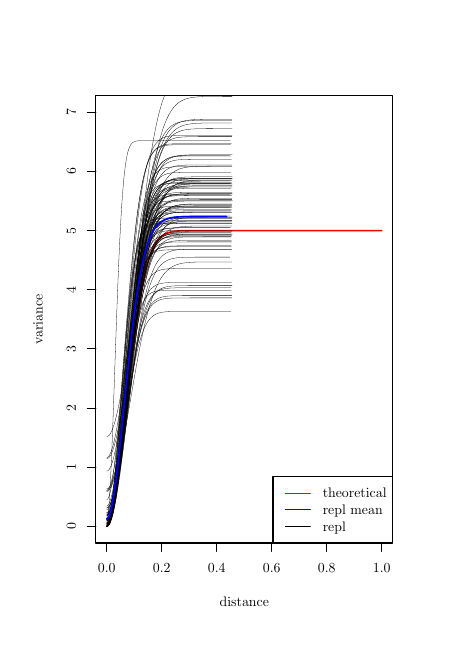
\begin{tikzpicture}[x=1pt,y=1pt]
\definecolor{fillColor}{RGB}{255,255,255}
\path[use as bounding box,fill=fillColor,fill opacity=0.00] (0,0) rectangle (144.54,216.81);
\begin{scope}
\path[clip] ( 24.60, 30.60) rectangle (131.94,192.21);
\definecolor{drawColor}{RGB}{255,0,0}

\path[draw=drawColor,line width= 0.6pt,line join=round,line cap=round] ( 28.58, 36.59) --
	( 29.58, 37.67) --
	( 30.58, 40.86) --
	( 31.59, 45.96) --
	( 32.59, 52.68) --
	( 33.60, 60.65) --
	( 34.60, 69.44) --
	( 35.60, 78.64) --
	( 36.61, 87.84) --
	( 37.61, 96.70) --
	( 38.61,104.94) --
	( 39.62,112.37) --
	( 40.62,118.88) --
	( 41.63,124.41) --
	( 42.63,129.00) --
	( 43.63,132.71) --
	( 44.64,135.63) --
	( 45.64,137.87) --
	( 46.65,139.55) --
	( 47.65,140.78) --
	( 48.65,141.67) --
	( 49.66,142.28) --
	( 50.66,142.70) --
	( 51.67,142.99) --
	( 52.67,143.17) --
	( 53.67,143.29) --
	( 54.68,143.36) --
	( 55.68,143.41) --
	( 56.69,143.43) --
	( 57.69,143.45) --
	( 58.69,143.46) --
	( 59.70,143.46) --
	( 60.70,143.47) --
	( 61.71,143.47) --
	( 62.71,143.47) --
	( 63.71,143.47) --
	( 64.72,143.47) --
	( 65.72,143.47) --
	( 66.72,143.47) --
	( 67.73,143.47) --
	( 68.73,143.47) --
	( 69.74,143.47) --
	( 70.74,143.47) --
	( 71.74,143.47) --
	( 72.75,143.47) --
	( 73.75,143.47) --
	( 74.76,143.47) --
	( 75.76,143.47) --
	( 76.76,143.47) --
	( 77.77,143.47) --
	( 78.77,143.47) --
	( 79.78,143.47) --
	( 80.78,143.47) --
	( 81.78,143.47) --
	( 82.79,143.47) --
	( 83.79,143.47) --
	( 84.80,143.47) --
	( 85.80,143.47) --
	( 86.80,143.47) --
	( 87.81,143.47) --
	( 88.81,143.47) --
	( 89.82,143.47) --
	( 90.82,143.47) --
	( 91.82,143.47) --
	( 92.83,143.47) --
	( 93.83,143.47) --
	( 94.83,143.47) --
	( 95.84,143.47) --
	( 96.84,143.47) --
	( 97.85,143.47) --
	( 98.85,143.47) --
	( 99.85,143.47) --
	(100.86,143.47) --
	(101.86,143.47) --
	(102.87,143.47) --
	(103.87,143.47) --
	(104.87,143.47) --
	(105.88,143.47) --
	(106.88,143.47) --
	(107.89,143.47) --
	(108.89,143.47) --
	(109.89,143.47) --
	(110.90,143.47) --
	(111.90,143.47) --
	(112.91,143.47) --
	(113.91,143.47) --
	(114.91,143.47) --
	(115.92,143.47) --
	(116.92,143.47) --
	(117.93,143.47) --
	(118.93,143.47) --
	(119.93,143.47) --
	(120.94,143.47) --
	(121.94,143.47) --
	(122.94,143.47) --
	(123.95,143.47) --
	(124.95,143.47) --
	(125.96,143.47) --
	(126.96,143.47) --
	(127.96,143.47);
\end{scope}
\begin{scope}
\path[clip] (  0.00,  0.00) rectangle (144.54,216.81);
\definecolor{drawColor}{RGB}{0,0,0}

\path[draw=drawColor,line width= 0.4pt,line join=round,line cap=round] ( 28.58, 30.60) -- (127.96, 30.60);

\path[draw=drawColor,line width= 0.4pt,line join=round,line cap=round] ( 28.58, 30.60) -- ( 28.58, 27.60);

\path[draw=drawColor,line width= 0.4pt,line join=round,line cap=round] ( 48.45, 30.60) -- ( 48.45, 27.60);

\path[draw=drawColor,line width= 0.4pt,line join=round,line cap=round] ( 68.33, 30.60) -- ( 68.33, 27.60);

\path[draw=drawColor,line width= 0.4pt,line join=round,line cap=round] ( 88.21, 30.60) -- ( 88.21, 27.60);

\path[draw=drawColor,line width= 0.4pt,line join=round,line cap=round] (108.09, 30.60) -- (108.09, 27.60);

\path[draw=drawColor,line width= 0.4pt,line join=round,line cap=round] (127.96, 30.60) -- (127.96, 27.60);

\node[text=drawColor,anchor=base,inner sep=0pt, outer sep=0pt, scale=  0.50] at ( 28.58, 19.80) {0.0};

\node[text=drawColor,anchor=base,inner sep=0pt, outer sep=0pt, scale=  0.50] at ( 48.45, 19.80) {0.2};

\node[text=drawColor,anchor=base,inner sep=0pt, outer sep=0pt, scale=  0.50] at ( 68.33, 19.80) {0.4};

\node[text=drawColor,anchor=base,inner sep=0pt, outer sep=0pt, scale=  0.50] at ( 88.21, 19.80) {0.6};

\node[text=drawColor,anchor=base,inner sep=0pt, outer sep=0pt, scale=  0.50] at (108.09, 19.80) {0.8};

\node[text=drawColor,anchor=base,inner sep=0pt, outer sep=0pt, scale=  0.50] at (127.96, 19.80) {1.0};

\path[draw=drawColor,line width= 0.4pt,line join=round,line cap=round] ( 24.60, 36.59) -- ( 24.60,186.22);

\path[draw=drawColor,line width= 0.4pt,line join=round,line cap=round] ( 24.60, 36.59) -- ( 21.60, 36.59);

\path[draw=drawColor,line width= 0.4pt,line join=round,line cap=round] ( 24.60, 57.96) -- ( 21.60, 57.96);

\path[draw=drawColor,line width= 0.4pt,line join=round,line cap=round] ( 24.60, 79.34) -- ( 21.60, 79.34);

\path[draw=drawColor,line width= 0.4pt,line join=round,line cap=round] ( 24.60,100.72) -- ( 21.60,100.72);

\path[draw=drawColor,line width= 0.4pt,line join=round,line cap=round] ( 24.60,122.09) -- ( 21.60,122.09);

\path[draw=drawColor,line width= 0.4pt,line join=round,line cap=round] ( 24.60,143.47) -- ( 21.60,143.47);

\path[draw=drawColor,line width= 0.4pt,line join=round,line cap=round] ( 24.60,164.85) -- ( 21.60,164.85);

\path[draw=drawColor,line width= 0.4pt,line join=round,line cap=round] ( 24.60,186.22) -- ( 21.60,186.22);

\node[text=drawColor,rotate= 90.00,anchor=base,inner sep=0pt, outer sep=0pt, scale=  0.50] at ( 17.40, 36.59) {0};

\node[text=drawColor,rotate= 90.00,anchor=base,inner sep=0pt, outer sep=0pt, scale=  0.50] at ( 17.40, 57.96) {1};

\node[text=drawColor,rotate= 90.00,anchor=base,inner sep=0pt, outer sep=0pt, scale=  0.50] at ( 17.40, 79.34) {2};

\node[text=drawColor,rotate= 90.00,anchor=base,inner sep=0pt, outer sep=0pt, scale=  0.50] at ( 17.40,100.72) {3};

\node[text=drawColor,rotate= 90.00,anchor=base,inner sep=0pt, outer sep=0pt, scale=  0.50] at ( 17.40,122.09) {4};

\node[text=drawColor,rotate= 90.00,anchor=base,inner sep=0pt, outer sep=0pt, scale=  0.50] at ( 17.40,143.47) {5};

\node[text=drawColor,rotate= 90.00,anchor=base,inner sep=0pt, outer sep=0pt, scale=  0.50] at ( 17.40,164.85) {6};

\node[text=drawColor,rotate= 90.00,anchor=base,inner sep=0pt, outer sep=0pt, scale=  0.50] at ( 17.40,186.22) {7};

\path[draw=drawColor,line width= 0.4pt,line join=round,line cap=round] ( 24.60, 30.60) --
	(131.94, 30.60) --
	(131.94,192.21) --
	( 24.60,192.21) --
	( 24.60, 30.60);
\end{scope}
\begin{scope}
\path[clip] (  0.00,  0.00) rectangle (144.54,216.81);
\definecolor{drawColor}{RGB}{0,0,0}

\node[text=drawColor,anchor=base,inner sep=0pt, outer sep=0pt, scale=  0.50] at ( 78.27,  7.80) {distance};

\node[text=drawColor,rotate= 90.00,anchor=base,inner sep=0pt, outer sep=0pt, scale=  0.50] at (  5.40,111.41) {variance};
\end{scope}
\begin{scope}
\path[clip] ( 24.60, 30.60) rectangle (131.94,192.21);
\definecolor{drawColor}{RGB}{0,0,0}

\path[draw=drawColor,line width= 0.1pt,line join=round,line cap=round] ( 28.58, 36.59) --
	( 28.80, 36.65) --
	( 29.03, 36.84) --
	( 29.26, 37.16) --
	( 29.48, 37.61) --
	( 29.71, 38.18) --
	( 29.94, 38.87) --
	( 30.16, 39.68) --
	( 30.39, 40.60) --
	( 30.62, 41.64) --
	( 30.84, 42.78) --
	( 31.07, 44.03) --
	( 31.29, 45.37) --
	( 31.52, 46.80) --
	( 31.75, 48.32) --
	( 31.97, 49.92) --
	( 32.20, 51.59) --
	( 32.43, 53.33) --
	( 32.65, 55.13) --
	( 32.88, 56.98) --
	( 33.11, 58.88) --
	( 33.33, 60.82) --
	( 33.56, 62.79) --
	( 33.79, 64.79) --
	( 34.01, 66.81) --
	( 34.24, 68.84) --
	( 34.47, 70.88) --
	( 34.69, 72.92) --
	( 34.92, 74.96) --
	( 35.15, 76.98) --
	( 35.37, 79.00) --
	( 35.60, 80.98) --
	( 35.83, 82.95) --
	( 36.05, 84.88) --
	( 36.28, 86.78) --
	( 36.51, 88.64) --
	( 36.73, 90.46) --
	( 36.96, 92.24) --
	( 37.19, 93.97) --
	( 37.41, 95.65) --
	( 37.64, 97.28) --
	( 37.87, 98.85) --
	( 38.09,100.37) --
	( 38.32,101.84) --
	( 38.55,103.24) --
	( 38.77,104.59) --
	( 39.00,105.89) --
	( 39.23,107.12) --
	( 39.45,108.30) --
	( 39.68,109.43) --
	( 39.91,110.49) --
	( 40.13,111.50) --
	( 40.36,112.46) --
	( 40.59,113.37) --
	( 40.81,114.22) --
	( 41.04,115.02) --
	( 41.27,115.78) --
	( 41.49,116.49) --
	( 41.72,117.15) --
	( 41.95,117.77) --
	( 42.17,118.35) --
	( 42.40,118.89) --
	( 42.62,119.39) --
	( 42.85,119.86) --
	( 43.08,120.29) --
	( 43.30,120.69) --
	( 43.53,121.06) --
	( 43.76,121.40) --
	( 43.98,121.72) --
	( 44.21,122.00) --
	( 44.44,122.27) --
	( 44.66,122.51) --
	( 44.89,122.73) --
	( 45.12,122.93) --
	( 45.34,123.12) --
	( 45.57,123.29) --
	( 45.80,123.44) --
	( 46.02,123.58) --
	( 46.25,123.70) --
	( 46.48,123.81) --
	( 46.70,123.92) --
	( 46.93,124.01) --
	( 47.16,124.09) --
	( 47.38,124.17) --
	( 47.61,124.23) --
	( 47.84,124.29) --
	( 48.06,124.35) --
	( 48.29,124.39) --
	( 48.52,124.44) --
	( 48.74,124.47) --
	( 48.97,124.51) --
	( 49.20,124.54) --
	( 49.42,124.56) --
	( 49.65,124.59) --
	( 49.88,124.61) --
	( 50.10,124.63) --
	( 50.33,124.64) --
	( 50.56,124.65) --
	( 50.78,124.67) --
	( 51.01,124.68) --
	( 51.24,124.69) --
	( 51.46,124.70) --
	( 51.69,124.70) --
	( 51.92,124.71) --
	( 52.14,124.71) --
	( 52.37,124.72) --
	( 52.60,124.72) --
	( 52.82,124.73) --
	( 53.05,124.73) --
	( 53.28,124.73) --
	( 53.50,124.73) --
	( 53.73,124.74) --
	( 53.96,124.74) --
	( 54.18,124.74) --
	( 54.41,124.74) --
	( 54.63,124.74) --
	( 54.86,124.74) --
	( 55.09,124.74) --
	( 55.31,124.74) --
	( 55.54,124.74) --
	( 55.77,124.75) --
	( 55.99,124.75) --
	( 56.22,124.75) --
	( 56.45,124.75) --
	( 56.67,124.75) --
	( 56.90,124.75) --
	( 57.13,124.75) --
	( 57.35,124.75) --
	( 57.58,124.75) --
	( 57.81,124.75) --
	( 58.03,124.75) --
	( 58.26,124.75) --
	( 58.49,124.75) --
	( 58.71,124.75) --
	( 58.94,124.75) --
	( 59.17,124.75) --
	( 59.39,124.75) --
	( 59.62,124.75) --
	( 59.85,124.75) --
	( 60.07,124.75) --
	( 60.30,124.75) --
	( 60.53,124.75) --
	( 60.75,124.75) --
	( 60.98,124.75) --
	( 61.21,124.75) --
	( 61.43,124.75) --
	( 61.66,124.75) --
	( 61.89,124.75) --
	( 62.11,124.75) --
	( 62.34,124.75) --
	( 62.57,124.75) --
	( 62.79,124.75) --
	( 63.02,124.75) --
	( 63.25,124.75) --
	( 63.47,124.75) --
	( 63.70,124.75) --
	( 63.93,124.75) --
	( 64.15,124.75) --
	( 64.38,124.75) --
	( 64.61,124.75) --
	( 64.83,124.75) --
	( 65.06,124.75) --
	( 65.29,124.75) --
	( 65.51,124.75) --
	( 65.74,124.75) --
	( 65.97,124.75) --
	( 66.19,124.75) --
	( 66.42,124.75) --
	( 66.64,124.75) --
	( 66.87,124.75) --
	( 67.10,124.75) --
	( 67.32,124.75) --
	( 67.55,124.75) --
	( 67.78,124.75) --
	( 68.00,124.75) --
	( 68.23,124.75) --
	( 68.46,124.75) --
	( 68.68,124.75) --
	( 68.91,124.75) --
	( 69.14,124.75) --
	( 69.36,124.75) --
	( 69.59,124.75) --
	( 69.82,124.75) --
	( 70.04,124.75) --
	( 70.27,124.75) --
	( 70.50,124.75) --
	( 70.72,124.75) --
	( 70.95,124.75) --
	( 71.18,124.75) --
	( 71.40,124.75) --
	( 71.63,124.75) --
	( 71.86,124.75) --
	( 72.08,124.75) --
	( 72.31,124.75) --
	( 72.54,124.75) --
	( 72.76,124.75) --
	( 72.99,124.75) --
	( 73.22,124.75) --
	( 73.44,124.75) --
	( 73.67,124.75);

\path[draw=drawColor,line width= 0.1pt,line join=round,line cap=round] ( 28.58, 36.59) --
	( 28.80, 36.63) --
	( 29.03, 36.77) --
	( 29.26, 37.01) --
	( 29.48, 37.34) --
	( 29.71, 37.76) --
	( 29.94, 38.28) --
	( 30.16, 38.88) --
	( 30.39, 39.57) --
	( 30.62, 40.35) --
	( 30.84, 41.21) --
	( 31.07, 42.15) --
	( 31.30, 43.18) --
	( 31.52, 44.27) --
	( 31.75, 45.45) --
	( 31.98, 46.69) --
	( 32.20, 48.00) --
	( 32.43, 49.37) --
	( 32.66, 50.81) --
	( 32.88, 52.30) --
	( 33.11, 53.84) --
	( 33.34, 55.43) --
	( 33.56, 57.07) --
	( 33.79, 58.74) --
	( 34.02, 60.46) --
	( 34.24, 62.20) --
	( 34.47, 63.98) --
	( 34.70, 65.78) --
	( 34.92, 67.60) --
	( 35.15, 69.44) --
	( 35.38, 71.29) --
	( 35.60, 73.15) --
	( 35.83, 75.02) --
	( 36.06, 76.88) --
	( 36.28, 78.75) --
	( 36.51, 80.61) --
	( 36.74, 82.46) --
	( 36.96, 84.31) --
	( 37.19, 86.13) --
	( 37.42, 87.94) --
	( 37.64, 89.73) --
	( 37.87, 91.50) --
	( 38.10, 93.24) --
	( 38.32, 94.95) --
	( 38.55, 96.64) --
	( 38.78, 98.29) --
	( 39.00, 99.91) --
	( 39.23,101.49) --
	( 39.46,103.04) --
	( 39.68,104.55) --
	( 39.91,106.03) --
	( 40.14,107.46) --
	( 40.36,108.85) --
	( 40.59,110.20) --
	( 40.82,111.51) --
	( 41.04,112.78) --
	( 41.27,114.01) --
	( 41.50,115.19) --
	( 41.72,116.33) --
	( 41.95,117.43) --
	( 42.18,118.49) --
	( 42.40,119.51) --
	( 42.63,120.48) --
	( 42.86,121.42) --
	( 43.08,122.31) --
	( 43.31,123.17) --
	( 43.54,123.98) --
	( 43.76,124.76) --
	( 43.99,125.51) --
	( 44.22,126.21) --
	( 44.44,126.88) --
	( 44.67,127.52) --
	( 44.90,128.13) --
	( 45.12,128.70) --
	( 45.35,129.24) --
	( 45.58,129.75) --
	( 45.80,130.24) --
	( 46.03,130.69) --
	( 46.26,131.12) --
	( 46.48,131.53) --
	( 46.71,131.91) --
	( 46.94,132.27) --
	( 47.16,132.60) --
	( 47.39,132.91) --
	( 47.62,133.21) --
	( 47.84,133.48) --
	( 48.07,133.74) --
	( 48.30,133.98) --
	( 48.52,134.20) --
	( 48.75,134.41) --
	( 48.98,134.60) --
	( 49.20,134.78) --
	( 49.43,134.94) --
	( 49.66,135.10) --
	( 49.88,135.24) --
	( 50.11,135.37) --
	( 50.34,135.49) --
	( 50.56,135.60) --
	( 50.79,135.71) --
	( 51.02,135.80) --
	( 51.24,135.89) --
	( 51.47,135.97) --
	( 51.70,136.05) --
	( 51.92,136.11) --
	( 52.15,136.18) --
	( 52.38,136.23) --
	( 52.60,136.28) --
	( 52.83,136.33) --
	( 53.06,136.38) --
	( 53.28,136.41) --
	( 53.51,136.45) --
	( 53.74,136.48) --
	( 53.96,136.51) --
	( 54.19,136.54) --
	( 54.42,136.56) --
	( 54.64,136.59) --
	( 54.87,136.61) --
	( 55.10,136.62) --
	( 55.32,136.64) --
	( 55.55,136.66) --
	( 55.78,136.67) --
	( 56.00,136.68) --
	( 56.23,136.69) --
	( 56.45,136.70) --
	( 56.68,136.71) --
	( 56.91,136.72) --
	( 57.13,136.73) --
	( 57.36,136.73) --
	( 57.59,136.74) --
	( 57.81,136.74) --
	( 58.04,136.75) --
	( 58.27,136.75) --
	( 58.49,136.75) --
	( 58.72,136.76) --
	( 58.95,136.76) --
	( 59.17,136.76) --
	( 59.40,136.76) --
	( 59.63,136.77) --
	( 59.85,136.77) --
	( 60.08,136.77) --
	( 60.31,136.77) --
	( 60.53,136.77) --
	( 60.76,136.77) --
	( 60.99,136.77) --
	( 61.21,136.77) --
	( 61.44,136.78) --
	( 61.67,136.78) --
	( 61.89,136.78) --
	( 62.12,136.78) --
	( 62.35,136.78) --
	( 62.57,136.78) --
	( 62.80,136.78) --
	( 63.03,136.78) --
	( 63.25,136.78) --
	( 63.48,136.78) --
	( 63.71,136.78) --
	( 63.93,136.78) --
	( 64.16,136.78) --
	( 64.39,136.78) --
	( 64.61,136.78) --
	( 64.84,136.78) --
	( 65.07,136.78) --
	( 65.29,136.78) --
	( 65.52,136.78) --
	( 65.75,136.78) --
	( 65.97,136.78) --
	( 66.20,136.78) --
	( 66.43,136.78) --
	( 66.65,136.78) --
	( 66.88,136.78) --
	( 67.11,136.78) --
	( 67.33,136.78) --
	( 67.56,136.78) --
	( 67.79,136.78) --
	( 68.01,136.78) --
	( 68.24,136.78) --
	( 68.47,136.78) --
	( 68.69,136.78) --
	( 68.92,136.78) --
	( 69.15,136.78) --
	( 69.37,136.78) --
	( 69.60,136.78) --
	( 69.83,136.78) --
	( 70.05,136.78) --
	( 70.28,136.78) --
	( 70.51,136.78) --
	( 70.73,136.78) --
	( 70.96,136.78) --
	( 71.19,136.78) --
	( 71.41,136.78) --
	( 71.64,136.78) --
	( 71.87,136.78) --
	( 72.09,136.78) --
	( 72.32,136.78) --
	( 72.55,136.78) --
	( 72.77,136.78) --
	( 73.00,136.78) --
	( 73.23,136.78) --
	( 73.45,136.78) --
	( 73.68,136.78);

\path[draw=drawColor,line width= 0.1pt,line join=round,line cap=round] ( 28.58, 61.06) --
	( 28.80, 61.10) --
	( 29.03, 61.20) --
	( 29.26, 61.37) --
	( 29.49, 61.61) --
	( 29.71, 61.91) --
	( 29.94, 62.29) --
	( 30.17, 62.72) --
	( 30.40, 63.23) --
	( 30.62, 63.79) --
	( 30.85, 64.42) --
	( 31.08, 65.11) --
	( 31.31, 65.86) --
	( 31.53, 66.66) --
	( 31.76, 67.52) --
	( 31.99, 68.43) --
	( 32.21, 69.39) --
	( 32.44, 70.41) --
	( 32.67, 71.46) --
	( 32.90, 72.57) --
	( 33.12, 73.71) --
	( 33.35, 74.89) --
	( 33.58, 76.12) --
	( 33.81, 77.37) --
	( 34.03, 78.66) --
	( 34.26, 79.97) --
	( 34.49, 81.31) --
	( 34.72, 82.68) --
	( 34.94, 84.06) --
	( 35.17, 85.46) --
	( 35.40, 86.88) --
	( 35.63, 88.31) --
	( 35.85, 89.75) --
	( 36.08, 91.20) --
	( 36.31, 92.65) --
	( 36.54, 94.11) --
	( 36.76, 95.57) --
	( 36.99, 97.02) --
	( 37.22, 98.47) --
	( 37.45, 99.91) --
	( 37.67,101.34) --
	( 37.90,102.77) --
	( 38.13,104.18) --
	( 38.36,105.57) --
	( 38.58,106.95) --
	( 38.81,108.31) --
	( 39.04,109.65) --
	( 39.27,110.97) --
	( 39.49,112.27) --
	( 39.72,113.54) --
	( 39.95,114.79) --
	( 40.18,116.02) --
	( 40.40,117.22) --
	( 40.63,118.39) --
	( 40.86,119.53) --
	( 41.09,120.64) --
	( 41.31,121.73) --
	( 41.54,122.78) --
	( 41.77,123.80) --
	( 42.00,124.80) --
	( 42.22,125.76) --
	( 42.45,126.70) --
	( 42.68,127.60) --
	( 42.90,128.47) --
	( 43.13,129.31) --
	( 43.36,130.12) --
	( 43.59,130.90) --
	( 43.81,131.66) --
	( 44.04,132.38) --
	( 44.27,133.07) --
	( 44.50,133.74) --
	( 44.72,134.38) --
	( 44.95,134.99) --
	( 45.18,135.57) --
	( 45.41,136.13) --
	( 45.63,136.66) --
	( 45.86,137.17) --
	( 46.09,137.65) --
	( 46.32,138.11) --
	( 46.54,138.54) --
	( 46.77,138.96) --
	( 47.00,139.35) --
	( 47.23,139.73) --
	( 47.45,140.08) --
	( 47.68,140.41) --
	( 47.91,140.73) --
	( 48.14,141.03) --
	( 48.36,141.31) --
	( 48.59,141.57) --
	( 48.82,141.82) --
	( 49.05,142.06) --
	( 49.27,142.28) --
	( 49.50,142.48) --
	( 49.73,142.68) --
	( 49.96,142.86) --
	( 50.18,143.03) --
	( 50.41,143.19) --
	( 50.64,143.34) --
	( 50.87,143.48) --
	( 51.09,143.61) --
	( 51.32,143.73) --
	( 51.55,143.84) --
	( 51.78,143.94) --
	( 52.00,144.04) --
	( 52.23,144.13) --
	( 52.46,144.21) --
	( 52.69,144.29) --
	( 52.91,144.36) --
	( 53.14,144.43) --
	( 53.37,144.49) --
	( 53.60,144.55) --
	( 53.82,144.60) --
	( 54.05,144.65) --
	( 54.28,144.69) --
	( 54.50,144.73) --
	( 54.73,144.77) --
	( 54.96,144.81) --
	( 55.19,144.84) --
	( 55.41,144.87) --
	( 55.64,144.89) --
	( 55.87,144.92) --
	( 56.10,144.94) --
	( 56.32,144.96) --
	( 56.55,144.98) --
	( 56.78,144.99) --
	( 57.01,145.01) --
	( 57.23,145.02) --
	( 57.46,145.04) --
	( 57.69,145.05) --
	( 57.92,145.06) --
	( 58.14,145.07) --
	( 58.37,145.08) --
	( 58.60,145.09) --
	( 58.83,145.09) --
	( 59.05,145.10) --
	( 59.28,145.10) --
	( 59.51,145.11) --
	( 59.74,145.11) --
	( 59.96,145.12) --
	( 60.19,145.12) --
	( 60.42,145.13) --
	( 60.65,145.13) --
	( 60.87,145.13) --
	( 61.10,145.13) --
	( 61.33,145.14) --
	( 61.56,145.14) --
	( 61.78,145.14) --
	( 62.01,145.14) --
	( 62.24,145.14) --
	( 62.47,145.14) --
	( 62.69,145.15) --
	( 62.92,145.15) --
	( 63.15,145.15) --
	( 63.38,145.15) --
	( 63.60,145.15) --
	( 63.83,145.15) --
	( 64.06,145.15) --
	( 64.29,145.15) --
	( 64.51,145.15) --
	( 64.74,145.15) --
	( 64.97,145.15) --
	( 65.20,145.15) --
	( 65.42,145.15) --
	( 65.65,145.15) --
	( 65.88,145.15) --
	( 66.10,145.15) --
	( 66.33,145.15) --
	( 66.56,145.15) --
	( 66.79,145.15) --
	( 67.01,145.15) --
	( 67.24,145.15) --
	( 67.47,145.15) --
	( 67.70,145.15) --
	( 67.92,145.15) --
	( 68.15,145.15) --
	( 68.38,145.15) --
	( 68.61,145.15) --
	( 68.83,145.15) --
	( 69.06,145.15) --
	( 69.29,145.15) --
	( 69.52,145.15) --
	( 69.74,145.15) --
	( 69.97,145.15) --
	( 70.20,145.15) --
	( 70.43,145.15) --
	( 70.65,145.15) --
	( 70.88,145.15) --
	( 71.11,145.15) --
	( 71.34,145.15) --
	( 71.56,145.15) --
	( 71.79,145.15) --
	( 72.02,145.15) --
	( 72.25,145.15) --
	( 72.47,145.15) --
	( 72.70,145.15) --
	( 72.93,145.15) --
	( 73.16,145.15) --
	( 73.38,145.15) --
	( 73.61,145.15) --
	( 73.84,145.15);

\path[draw=drawColor,line width= 0.1pt,line join=round,line cap=round] ( 28.58, 49.16) --
	( 28.80, 49.20) --
	( 29.02, 49.32) --
	( 29.25, 49.53) --
	( 29.47, 49.81) --
	( 29.70, 50.18) --
	( 29.92, 50.62) --
	( 30.14, 51.14) --
	( 30.37, 51.74) --
	( 30.59, 52.41) --
	( 30.82, 53.16) --
	( 31.04, 53.99) --
	( 31.26, 54.88) --
	( 31.49, 55.84) --
	( 31.71, 56.87) --
	( 31.94, 57.97) --
	( 32.16, 59.13) --
	( 32.39, 60.34) --
	( 32.61, 61.62) --
	( 32.83, 62.95) --
	( 33.06, 64.34) --
	( 33.28, 65.77) --
	( 33.51, 67.25) --
	( 33.73, 68.78) --
	( 33.95, 70.35) --
	( 34.18, 71.95) --
	( 34.40, 73.59) --
	( 34.63, 75.27) --
	( 34.85, 76.97) --
	( 35.07, 78.70) --
	( 35.30, 80.45) --
	( 35.52, 82.23) --
	( 35.75, 84.02) --
	( 35.97, 85.82) --
	( 36.20, 87.64) --
	( 36.42, 89.47) --
	( 36.64, 91.30) --
	( 36.87, 93.13) --
	( 37.09, 94.96) --
	( 37.32, 96.80) --
	( 37.54, 98.62) --
	( 37.76,100.44) --
	( 37.99,102.25) --
	( 38.21,104.05) --
	( 38.44,105.83) --
	( 38.66,107.60) --
	( 38.88,109.35) --
	( 39.11,111.08) --
	( 39.33,112.79) --
	( 39.56,114.47) --
	( 39.78,116.13) --
	( 40.01,117.76) --
	( 40.23,119.36) --
	( 40.45,120.93) --
	( 40.68,122.47) --
	( 40.90,123.98) --
	( 41.13,125.46) --
	( 41.35,126.91) --
	( 41.57,128.32) --
	( 41.80,129.69) --
	( 42.02,131.03) --
	( 42.25,132.34) --
	( 42.47,133.61) --
	( 42.69,134.84) --
	( 42.92,136.04) --
	( 43.14,137.20) --
	( 43.37,138.32) --
	( 43.59,139.41) --
	( 43.82,140.46) --
	( 44.04,141.48) --
	( 44.26,142.46) --
	( 44.49,143.40) --
	( 44.71,144.31) --
	( 44.94,145.19) --
	( 45.16,146.03) --
	( 45.38,146.84) --
	( 45.61,147.62) --
	( 45.83,148.36) --
	( 46.06,149.08) --
	( 46.28,149.76) --
	( 46.50,150.41) --
	( 46.73,151.04) --
	( 46.95,151.63) --
	( 47.18,152.20) --
	( 47.40,152.74) --
	( 47.63,153.26) --
	( 47.85,153.75) --
	( 48.07,154.21) --
	( 48.30,154.65) --
	( 48.52,155.07) --
	( 48.75,155.47) --
	( 48.97,155.85) --
	( 49.19,156.20) --
	( 49.42,156.54) --
	( 49.64,156.86) --
	( 49.87,157.16) --
	( 50.09,157.44) --
	( 50.31,157.71) --
	( 50.54,157.96) --
	( 50.76,158.20) --
	( 50.99,158.42) --
	( 51.21,158.63) --
	( 51.44,158.83) --
	( 51.66,159.01) --
	( 51.88,159.18) --
	( 52.11,159.35) --
	( 52.33,159.50) --
	( 52.56,159.64) --
	( 52.78,159.77) --
	( 53.00,159.89) --
	( 53.23,160.01) --
	( 53.45,160.11) --
	( 53.68,160.21) --
	( 53.90,160.31) --
	( 54.12,160.39) --
	( 54.35,160.47) --
	( 54.57,160.55) --
	( 54.80,160.61) --
	( 55.02,160.68) --
	( 55.25,160.74) --
	( 55.47,160.79) --
	( 55.69,160.84) --
	( 55.92,160.89) --
	( 56.14,160.93) --
	( 56.37,160.97) --
	( 56.59,161.01) --
	( 56.81,161.04) --
	( 57.04,161.07) --
	( 57.26,161.10) --
	( 57.49,161.13) --
	( 57.71,161.15) --
	( 57.93,161.17) --
	( 58.16,161.19) --
	( 58.38,161.21) --
	( 58.61,161.23) --
	( 58.83,161.24) --
	( 59.06,161.26) --
	( 59.28,161.27) --
	( 59.50,161.28) --
	( 59.73,161.29) --
	( 59.95,161.30) --
	( 60.18,161.31) --
	( 60.40,161.32) --
	( 60.62,161.33) --
	( 60.85,161.33) --
	( 61.07,161.34) --
	( 61.30,161.34) --
	( 61.52,161.35) --
	( 61.74,161.35) --
	( 61.97,161.36) --
	( 62.19,161.36) --
	( 62.42,161.36) --
	( 62.64,161.37) --
	( 62.87,161.37) --
	( 63.09,161.37) --
	( 63.31,161.37) --
	( 63.54,161.38) --
	( 63.76,161.38) --
	( 63.99,161.38) --
	( 64.21,161.38) --
	( 64.43,161.38) --
	( 64.66,161.38) --
	( 64.88,161.38) --
	( 65.11,161.39) --
	( 65.33,161.39) --
	( 65.55,161.39) --
	( 65.78,161.39) --
	( 66.00,161.39) --
	( 66.23,161.39) --
	( 66.45,161.39) --
	( 66.68,161.39) --
	( 66.90,161.39) --
	( 67.12,161.39) --
	( 67.35,161.39) --
	( 67.57,161.39) --
	( 67.80,161.39) --
	( 68.02,161.39) --
	( 68.24,161.39) --
	( 68.47,161.39) --
	( 68.69,161.39) --
	( 68.92,161.39) --
	( 69.14,161.39) --
	( 69.36,161.39) --
	( 69.59,161.39) --
	( 69.81,161.39) --
	( 70.04,161.39) --
	( 70.26,161.39) --
	( 70.49,161.39) --
	( 70.71,161.39) --
	( 70.93,161.39) --
	( 71.16,161.39) --
	( 71.38,161.39) --
	( 71.61,161.39) --
	( 71.83,161.39) --
	( 72.05,161.39) --
	( 72.28,161.39) --
	( 72.50,161.39) --
	( 72.73,161.39) --
	( 72.95,161.39) --
	( 73.17,161.39);

\path[draw=drawColor,line width= 0.1pt,line join=round,line cap=round] ( 28.58, 43.19) --
	( 28.80, 43.23) --
	( 29.02, 43.36) --
	( 29.24, 43.58) --
	( 29.47, 43.88) --
	( 29.69, 44.27) --
	( 29.91, 44.74) --
	( 30.14, 45.29) --
	( 30.36, 45.93) --
	( 30.58, 46.65) --
	( 30.81, 47.44) --
	( 31.03, 48.31) --
	( 31.25, 49.26) --
	( 31.47, 50.29) --
	( 31.70, 51.38) --
	( 31.92, 52.54) --
	( 32.14, 53.77) --
	( 32.37, 55.06) --
	( 32.59, 56.42) --
	( 32.81, 57.83) --
	( 33.04, 59.30) --
	( 33.26, 60.82) --
	( 33.48, 62.39) --
	( 33.71, 64.01) --
	( 33.93, 65.67) --
	( 34.15, 67.37) --
	( 34.37, 69.10) --
	( 34.60, 70.88) --
	( 34.82, 72.68) --
	( 35.04, 74.51) --
	( 35.27, 76.36) --
	( 35.49, 78.23) --
	( 35.71, 80.13) --
	( 35.94, 82.03) --
	( 36.16, 83.95) --
	( 36.38, 85.88) --
	( 36.60, 87.81) --
	( 36.83, 89.74) --
	( 37.05, 91.67) --
	( 37.27, 93.60) --
	( 37.50, 95.53) --
	( 37.72, 97.44) --
	( 37.94, 99.35) --
	( 38.17,101.24) --
	( 38.39,103.11) --
	( 38.61,104.97) --
	( 38.83,106.80) --
	( 39.06,108.61) --
	( 39.28,110.40) --
	( 39.50,112.17) --
	( 39.73,113.90) --
	( 39.95,115.61) --
	( 40.17,117.28) --
	( 40.40,118.93) --
	( 40.62,120.54) --
	( 40.84,122.12) --
	( 41.06,123.66) --
	( 41.29,125.17) --
	( 41.51,126.63) --
	( 41.73,128.07) --
	( 41.96,129.46) --
	( 42.18,130.82) --
	( 42.40,132.14) --
	( 42.63,133.42) --
	( 42.85,134.66) --
	( 43.07,135.86) --
	( 43.30,137.03) --
	( 43.52,138.15) --
	( 43.74,139.24) --
	( 43.96,140.29) --
	( 44.19,141.30) --
	( 44.41,142.28) --
	( 44.63,143.22) --
	( 44.86,144.12) --
	( 45.08,144.98) --
	( 45.30,145.82) --
	( 45.53,146.61) --
	( 45.75,147.38) --
	( 45.97,148.11) --
	( 46.19,148.81) --
	( 46.42,149.48) --
	( 46.64,150.11) --
	( 46.86,150.72) --
	( 47.09,151.30) --
	( 47.31,151.85) --
	( 47.53,152.38) --
	( 47.76,152.87) --
	( 47.98,153.35) --
	( 48.20,153.80) --
	( 48.42,154.22) --
	( 48.65,154.62) --
	( 48.87,155.01) --
	( 49.09,155.37) --
	( 49.32,155.71) --
	( 49.54,156.03) --
	( 49.76,156.33) --
	( 49.99,156.62) --
	( 50.21,156.88) --
	( 50.43,157.14) --
	( 50.65,157.37) --
	( 50.88,157.60) --
	( 51.10,157.81) --
	( 51.32,158.00) --
	( 51.55,158.19) --
	( 51.77,158.36) --
	( 51.99,158.52) --
	( 52.22,158.67) --
	( 52.44,158.81) --
	( 52.66,158.94) --
	( 52.88,159.06) --
	( 53.11,159.18) --
	( 53.33,159.28) --
	( 53.55,159.38) --
	( 53.78,159.47) --
	( 54.00,159.55) --
	( 54.22,159.63) --
	( 54.45,159.71) --
	( 54.67,159.77) --
	( 54.89,159.84) --
	( 55.12,159.89) --
	( 55.34,159.95) --
	( 55.56,159.99) --
	( 55.78,160.04) --
	( 56.01,160.08) --
	( 56.23,160.12) --
	( 56.45,160.16) --
	( 56.68,160.19) --
	( 56.90,160.22) --
	( 57.12,160.25) --
	( 57.35,160.27) --
	( 57.57,160.29) --
	( 57.79,160.31) --
	( 58.01,160.33) --
	( 58.24,160.35) --
	( 58.46,160.37) --
	( 58.68,160.38) --
	( 58.91,160.40) --
	( 59.13,160.41) --
	( 59.35,160.42) --
	( 59.58,160.43) --
	( 59.80,160.44) --
	( 60.02,160.45) --
	( 60.24,160.45) --
	( 60.47,160.46) --
	( 60.69,160.47) --
	( 60.91,160.47) --
	( 61.14,160.48) --
	( 61.36,160.48) --
	( 61.58,160.49) --
	( 61.81,160.49) --
	( 62.03,160.49) --
	( 62.25,160.50) --
	( 62.47,160.50) --
	( 62.70,160.50) --
	( 62.92,160.50) --
	( 63.14,160.51) --
	( 63.37,160.51) --
	( 63.59,160.51) --
	( 63.81,160.51) --
	( 64.04,160.51) --
	( 64.26,160.51) --
	( 64.48,160.51) --
	( 64.71,160.51) --
	( 64.93,160.52) --
	( 65.15,160.52) --
	( 65.37,160.52) --
	( 65.60,160.52) --
	( 65.82,160.52) --
	( 66.04,160.52) --
	( 66.27,160.52) --
	( 66.49,160.52) --
	( 66.71,160.52) --
	( 66.94,160.52) --
	( 67.16,160.52) --
	( 67.38,160.52) --
	( 67.60,160.52) --
	( 67.83,160.52) --
	( 68.05,160.52) --
	( 68.27,160.52) --
	( 68.50,160.52) --
	( 68.72,160.52) --
	( 68.94,160.52) --
	( 69.17,160.52) --
	( 69.39,160.52) --
	( 69.61,160.52) --
	( 69.83,160.52) --
	( 70.06,160.52) --
	( 70.28,160.52) --
	( 70.50,160.52) --
	( 70.73,160.52) --
	( 70.95,160.52) --
	( 71.17,160.52) --
	( 71.40,160.52) --
	( 71.62,160.52) --
	( 71.84,160.52) --
	( 72.06,160.52) --
	( 72.29,160.52) --
	( 72.51,160.52) --
	( 72.73,160.52) --
	( 72.96,160.52);

\path[draw=drawColor,line width= 0.1pt,line join=round,line cap=round] ( 28.58, 39.19) --
	( 28.80, 39.25) --
	( 29.03, 39.45) --
	( 29.26, 39.77) --
	( 29.48, 40.22) --
	( 29.71, 40.80) --
	( 29.94, 41.50) --
	( 30.16, 42.32) --
	( 30.39, 43.27) --
	( 30.62, 44.32) --
	( 30.84, 45.49) --
	( 31.07, 46.77) --
	( 31.30, 48.15) --
	( 31.52, 49.63) --
	( 31.75, 51.20) --
	( 31.98, 52.86) --
	( 32.20, 54.60) --
	( 32.43, 56.42) --
	( 32.66, 58.32) --
	( 32.89, 60.27) --
	( 33.11, 62.29) --
	( 33.34, 64.36) --
	( 33.57, 66.47) --
	( 33.79, 68.63) --
	( 34.02, 70.82) --
	( 34.25, 73.04) --
	( 34.47, 75.28) --
	( 34.70, 77.54) --
	( 34.93, 79.80) --
	( 35.15, 82.08) --
	( 35.38, 84.35) --
	( 35.61, 86.61) --
	( 35.83, 88.87) --
	( 36.06, 91.10) --
	( 36.29, 93.32) --
	( 36.51, 95.51) --
	( 36.74, 97.67) --
	( 36.97, 99.80) --
	( 37.20,101.89) --
	( 37.42,103.94) --
	( 37.65,105.95) --
	( 37.88,107.92) --
	( 38.10,109.83) --
	( 38.33,111.69) --
	( 38.56,113.50) --
	( 38.78,115.26) --
	( 39.01,116.96) --
	( 39.24,118.61) --
	( 39.46,120.20) --
	( 39.69,121.73) --
	( 39.92,123.20) --
	( 40.14,124.62) --
	( 40.37,125.98) --
	( 40.60,127.28) --
	( 40.82,128.52) --
	( 41.05,129.71) --
	( 41.28,130.84) --
	( 41.50,131.92) --
	( 41.73,132.94) --
	( 41.96,133.91) --
	( 42.19,134.83) --
	( 42.41,135.70) --
	( 42.64,136.52) --
	( 42.87,137.30) --
	( 43.09,138.03) --
	( 43.32,138.71) --
	( 43.55,139.36) --
	( 43.77,139.96) --
	( 44.00,140.53) --
	( 44.23,141.06) --
	( 44.45,141.55) --
	( 44.68,142.01) --
	( 44.91,142.44) --
	( 45.13,142.84) --
	( 45.36,143.21) --
	( 45.59,143.56) --
	( 45.81,143.88) --
	( 46.04,144.17) --
	( 46.27,144.44) --
	( 46.50,144.69) --
	( 46.72,144.92) --
	( 46.95,145.14) --
	( 47.18,145.33) --
	( 47.40,145.51) --
	( 47.63,145.67) --
	( 47.86,145.82) --
	( 48.08,145.96) --
	( 48.31,146.09) --
	( 48.54,146.20) --
	( 48.76,146.30) --
	( 48.99,146.40) --
	( 49.22,146.48) --
	( 49.44,146.56) --
	( 49.67,146.63) --
	( 49.90,146.69) --
	( 50.12,146.75) --
	( 50.35,146.80) --
	( 50.58,146.85) --
	( 50.80,146.89) --
	( 51.03,146.93) --
	( 51.26,146.96) --
	( 51.49,146.99) --
	( 51.71,147.02) --
	( 51.94,147.04) --
	( 52.17,147.06) --
	( 52.39,147.08) --
	( 52.62,147.10) --
	( 52.85,147.11) --
	( 53.07,147.13) --
	( 53.30,147.14) --
	( 53.53,147.15) --
	( 53.75,147.16) --
	( 53.98,147.17) --
	( 54.21,147.17) --
	( 54.43,147.18) --
	( 54.66,147.19) --
	( 54.89,147.19) --
	( 55.11,147.20) --
	( 55.34,147.20) --
	( 55.57,147.20) --
	( 55.80,147.21) --
	( 56.02,147.21) --
	( 56.25,147.21) --
	( 56.48,147.21) --
	( 56.70,147.21) --
	( 56.93,147.22) --
	( 57.16,147.22) --
	( 57.38,147.22) --
	( 57.61,147.22) --
	( 57.84,147.22) --
	( 58.06,147.22) --
	( 58.29,147.22) --
	( 58.52,147.22) --
	( 58.74,147.22) --
	( 58.97,147.22) --
	( 59.20,147.22) --
	( 59.42,147.22) --
	( 59.65,147.22) --
	( 59.88,147.22) --
	( 60.10,147.22) --
	( 60.33,147.22) --
	( 60.56,147.22) --
	( 60.79,147.22) --
	( 61.01,147.22) --
	( 61.24,147.22) --
	( 61.47,147.22) --
	( 61.69,147.22) --
	( 61.92,147.22) --
	( 62.15,147.22) --
	( 62.37,147.22) --
	( 62.60,147.22) --
	( 62.83,147.22) --
	( 63.05,147.22) --
	( 63.28,147.22) --
	( 63.51,147.22) --
	( 63.73,147.22) --
	( 63.96,147.22) --
	( 64.19,147.22) --
	( 64.41,147.22) --
	( 64.64,147.22) --
	( 64.87,147.22) --
	( 65.10,147.22) --
	( 65.32,147.22) --
	( 65.55,147.22) --
	( 65.78,147.22) --
	( 66.00,147.22) --
	( 66.23,147.22) --
	( 66.46,147.22) --
	( 66.68,147.22) --
	( 66.91,147.22) --
	( 67.14,147.22) --
	( 67.36,147.22) --
	( 67.59,147.22) --
	( 67.82,147.22) --
	( 68.04,147.22) --
	( 68.27,147.22) --
	( 68.50,147.22) --
	( 68.72,147.22) --
	( 68.95,147.22) --
	( 69.18,147.22) --
	( 69.40,147.22) --
	( 69.63,147.22) --
	( 69.86,147.22) --
	( 70.09,147.22) --
	( 70.31,147.22) --
	( 70.54,147.22) --
	( 70.77,147.22) --
	( 70.99,147.22) --
	( 71.22,147.22) --
	( 71.45,147.22) --
	( 71.67,147.22) --
	( 71.90,147.22) --
	( 72.13,147.22) --
	( 72.35,147.22) --
	( 72.58,147.22) --
	( 72.81,147.22) --
	( 73.03,147.22) --
	( 73.26,147.22) --
	( 73.49,147.22) --
	( 73.71,147.22);

\path[draw=drawColor,line width= 0.1pt,line join=round,line cap=round] ( 28.58, 37.78) --
	( 28.80, 37.84) --
	( 29.03, 38.02) --
	( 29.26, 38.32) --
	( 29.49, 38.73) --
	( 29.71, 39.27) --
	( 29.94, 39.92) --
	( 30.17, 40.68) --
	( 30.40, 41.55) --
	( 30.63, 42.53) --
	( 30.85, 43.62) --
	( 31.08, 44.80) --
	( 31.31, 46.09) --
	( 31.54, 47.47) --
	( 31.77, 48.95) --
	( 31.99, 50.51) --
	( 32.22, 52.15) --
	( 32.45, 53.87) --
	( 32.68, 55.67) --
	( 32.91, 57.53) --
	( 33.13, 59.46) --
	( 33.36, 61.44) --
	( 33.59, 63.48) --
	( 33.82, 65.57) --
	( 34.04, 67.70) --
	( 34.27, 69.87) --
	( 34.50, 72.07) --
	( 34.73, 74.29) --
	( 34.96, 76.54) --
	( 35.18, 78.81) --
	( 35.41, 81.09) --
	( 35.64, 83.38) --
	( 35.87, 85.67) --
	( 36.10, 87.95) --
	( 36.32, 90.23) --
	( 36.55, 92.50) --
	( 36.78, 94.76) --
	( 37.01, 96.99) --
	( 37.23, 99.21) --
	( 37.46,101.39) --
	( 37.69,103.55) --
	( 37.92,105.68) --
	( 38.15,107.77) --
	( 38.37,109.82) --
	( 38.60,111.83) --
	( 38.83,113.80) --
	( 39.06,115.73) --
	( 39.29,117.60) --
	( 39.51,119.43) --
	( 39.74,121.21) --
	( 39.97,122.94) --
	( 40.20,124.62) --
	( 40.43,126.25) --
	( 40.65,127.82) --
	( 40.88,129.34) --
	( 41.11,130.81) --
	( 41.34,132.22) --
	( 41.56,133.58) --
	( 41.79,134.89) --
	( 42.02,136.14) --
	( 42.25,137.34) --
	( 42.48,138.49) --
	( 42.70,139.59) --
	( 42.93,140.65) --
	( 43.16,141.65) --
	( 43.39,142.60) --
	( 43.62,143.51) --
	( 43.84,144.37) --
	( 44.07,145.19) --
	( 44.30,145.97) --
	( 44.53,146.70) --
	( 44.75,147.40) --
	( 44.98,148.06) --
	( 45.21,148.67) --
	( 45.44,149.26) --
	( 45.67,149.81) --
	( 45.89,150.32) --
	( 46.12,150.81) --
	( 46.35,151.26) --
	( 46.58,151.69) --
	( 46.81,152.08) --
	( 47.03,152.45) --
	( 47.26,152.80) --
	( 47.49,153.12) --
	( 47.72,153.43) --
	( 47.95,153.71) --
	( 48.17,153.97) --
	( 48.40,154.21) --
	( 48.63,154.43) --
	( 48.86,154.64) --
	( 49.08,154.83) --
	( 49.31,155.01) --
	( 49.54,155.17) --
	( 49.77,155.32) --
	( 50.00,155.46) --
	( 50.22,155.59) --
	( 50.45,155.70) --
	( 50.68,155.81) --
	( 50.91,155.91) --
	( 51.14,156.00) --
	( 51.36,156.08) --
	( 51.59,156.16) --
	( 51.82,156.23) --
	( 52.05,156.29) --
	( 52.27,156.35) --
	( 52.50,156.40) --
	( 52.73,156.45) --
	( 52.96,156.49) --
	( 53.19,156.53) --
	( 53.41,156.56) --
	( 53.64,156.59) --
	( 53.87,156.62) --
	( 54.10,156.65) --
	( 54.33,156.67) --
	( 54.55,156.69) --
	( 54.78,156.71) --
	( 55.01,156.73) --
	( 55.24,156.74) --
	( 55.46,156.76) --
	( 55.69,156.77) --
	( 55.92,156.78) --
	( 56.15,156.79) --
	( 56.38,156.80) --
	( 56.60,156.81) --
	( 56.83,156.81) --
	( 57.06,156.82) --
	( 57.29,156.83) --
	( 57.52,156.83) --
	( 57.74,156.84) --
	( 57.97,156.84) --
	( 58.20,156.84) --
	( 58.43,156.85) --
	( 58.66,156.85) --
	( 58.88,156.85) --
	( 59.11,156.85) --
	( 59.34,156.85) --
	( 59.57,156.86) --
	( 59.79,156.86) --
	( 60.02,156.86) --
	( 60.25,156.86) --
	( 60.48,156.86) --
	( 60.71,156.86) --
	( 60.93,156.86) --
	( 61.16,156.86) --
	( 61.39,156.86) --
	( 61.62,156.86) --
	( 61.85,156.86) --
	( 62.07,156.86) --
	( 62.30,156.86) --
	( 62.53,156.87) --
	( 62.76,156.87) --
	( 62.98,156.87) --
	( 63.21,156.87) --
	( 63.44,156.87) --
	( 63.67,156.87) --
	( 63.90,156.87) --
	( 64.12,156.87) --
	( 64.35,156.87) --
	( 64.58,156.87) --
	( 64.81,156.87) --
	( 65.04,156.87) --
	( 65.26,156.87) --
	( 65.49,156.87) --
	( 65.72,156.87) --
	( 65.95,156.87) --
	( 66.18,156.87) --
	( 66.40,156.87) --
	( 66.63,156.87) --
	( 66.86,156.87) --
	( 67.09,156.87) --
	( 67.31,156.87) --
	( 67.54,156.87) --
	( 67.77,156.87) --
	( 68.00,156.87) --
	( 68.23,156.87) --
	( 68.45,156.87) --
	( 68.68,156.87) --
	( 68.91,156.87) --
	( 69.14,156.87) --
	( 69.37,156.87) --
	( 69.59,156.87) --
	( 69.82,156.87) --
	( 70.05,156.87) --
	( 70.28,156.87) --
	( 70.50,156.87) --
	( 70.73,156.87) --
	( 70.96,156.87) --
	( 71.19,156.87) --
	( 71.42,156.87) --
	( 71.64,156.87) --
	( 71.87,156.87) --
	( 72.10,156.87) --
	( 72.33,156.87) --
	( 72.56,156.87) --
	( 72.78,156.87) --
	( 73.01,156.87) --
	( 73.24,156.87) --
	( 73.47,156.87) --
	( 73.70,156.87) --
	( 73.92,156.87);

\path[draw=drawColor,line width= 0.1pt,line join=round,line cap=round] ( 28.58, 36.59) --
	( 28.80, 36.65) --
	( 29.03, 36.85) --
	( 29.26, 37.17) --
	( 29.48, 37.63) --
	( 29.71, 38.21) --
	( 29.94, 38.92) --
	( 30.16, 39.75) --
	( 30.39, 40.69) --
	( 30.61, 41.75) --
	( 30.84, 42.92) --
	( 31.07, 44.20) --
	( 31.29, 45.57) --
	( 31.52, 47.04) --
	( 31.75, 48.60) --
	( 31.97, 50.24) --
	( 32.20, 51.96) --
	( 32.43, 53.75) --
	( 32.65, 55.60) --
	( 32.88, 57.51) --
	( 33.11, 59.47) --
	( 33.33, 61.47) --
	( 33.56, 63.51) --
	( 33.79, 65.57) --
	( 34.01, 67.66) --
	( 34.24, 69.77) --
	( 34.47, 71.89) --
	( 34.69, 74.01) --
	( 34.92, 76.13) --
	( 35.15, 78.24) --
	( 35.37, 80.34) --
	( 35.60, 82.42) --
	( 35.83, 84.47) --
	( 36.05, 86.50) --
	( 36.28, 88.49) --
	( 36.51, 90.45) --
	( 36.73, 92.37) --
	( 36.96, 94.24) --
	( 37.19, 96.07) --
	( 37.41, 97.85) --
	( 37.64, 99.58) --
	( 37.87,101.25) --
	( 38.09,102.87) --
	( 38.32,104.44) --
	( 38.55,105.94) --
	( 38.77,107.39) --
	( 39.00,108.78) --
	( 39.23,110.11) --
	( 39.45,111.38) --
	( 39.68,112.60) --
	( 39.90,113.75) --
	( 40.13,114.85) --
	( 40.36,115.90) --
	( 40.58,116.89) --
	( 40.81,117.82) --
	( 41.04,118.71) --
	( 41.26,119.54) --
	( 41.49,120.32) --
	( 41.72,121.06) --
	( 41.94,121.75) --
	( 42.17,122.39) --
	( 42.40,122.99) --
	( 42.62,123.56) --
	( 42.85,124.08) --
	( 43.08,124.57) --
	( 43.30,125.02) --
	( 43.53,125.44) --
	( 43.76,125.83) --
	( 43.98,126.18) --
	( 44.21,126.51) --
	( 44.44,126.82) --
	( 44.66,127.10) --
	( 44.89,127.35) --
	( 45.12,127.59) --
	( 45.34,127.80) --
	( 45.57,128.00) --
	( 45.80,128.18) --
	( 46.02,128.34) --
	( 46.25,128.49) --
	( 46.48,128.62) --
	( 46.70,128.75) --
	( 46.93,128.86) --
	( 47.16,128.96) --
	( 47.38,129.05) --
	( 47.61,129.13) --
	( 47.84,129.20) --
	( 48.06,129.26) --
	( 48.29,129.32) --
	( 48.52,129.37) --
	( 48.74,129.42) --
	( 48.97,129.46) --
	( 49.19,129.50) --
	( 49.42,129.53) --
	( 49.65,129.56) --
	( 49.87,129.59) --
	( 50.10,129.61) --
	( 50.33,129.63) --
	( 50.55,129.65) --
	( 50.78,129.67) --
	( 51.01,129.68) --
	( 51.23,129.69) --
	( 51.46,129.70) --
	( 51.69,129.71) --
	( 51.91,129.72) --
	( 52.14,129.73) --
	( 52.37,129.73) --
	( 52.59,129.74) --
	( 52.82,129.74) --
	( 53.05,129.75) --
	( 53.27,129.75) --
	( 53.50,129.75) --
	( 53.73,129.76) --
	( 53.95,129.76) --
	( 54.18,129.76) --
	( 54.41,129.76) --
	( 54.63,129.76) --
	( 54.86,129.77) --
	( 55.09,129.77) --
	( 55.31,129.77) --
	( 55.54,129.77) --
	( 55.77,129.77) --
	( 55.99,129.77) --
	( 56.22,129.77) --
	( 56.45,129.77) --
	( 56.67,129.77) --
	( 56.90,129.77) --
	( 57.13,129.77) --
	( 57.35,129.77) --
	( 57.58,129.77) --
	( 57.81,129.77) --
	( 58.03,129.77) --
	( 58.26,129.77) --
	( 58.48,129.77) --
	( 58.71,129.77) --
	( 58.94,129.77) --
	( 59.16,129.77) --
	( 59.39,129.77) --
	( 59.62,129.77) --
	( 59.84,129.77) --
	( 60.07,129.77) --
	( 60.30,129.77) --
	( 60.52,129.77) --
	( 60.75,129.77) --
	( 60.98,129.77) --
	( 61.20,129.77) --
	( 61.43,129.77) --
	( 61.66,129.77) --
	( 61.88,129.77) --
	( 62.11,129.77) --
	( 62.34,129.77) --
	( 62.56,129.77) --
	( 62.79,129.77) --
	( 63.02,129.77) --
	( 63.24,129.77) --
	( 63.47,129.77) --
	( 63.70,129.77) --
	( 63.92,129.77) --
	( 64.15,129.77) --
	( 64.38,129.77) --
	( 64.60,129.77) --
	( 64.83,129.77) --
	( 65.06,129.77) --
	( 65.28,129.77) --
	( 65.51,129.77) --
	( 65.74,129.77) --
	( 65.96,129.77) --
	( 66.19,129.77) --
	( 66.42,129.77) --
	( 66.64,129.77) --
	( 66.87,129.77) --
	( 67.10,129.77) --
	( 67.32,129.77) --
	( 67.55,129.77) --
	( 67.77,129.77) --
	( 68.00,129.77) --
	( 68.23,129.77) --
	( 68.45,129.77) --
	( 68.68,129.77) --
	( 68.91,129.77) --
	( 69.13,129.77) --
	( 69.36,129.77) --
	( 69.59,129.77) --
	( 69.81,129.77) --
	( 70.04,129.77) --
	( 70.27,129.77) --
	( 70.49,129.77) --
	( 70.72,129.77) --
	( 70.95,129.77) --
	( 71.17,129.77) --
	( 71.40,129.77) --
	( 71.63,129.77) --
	( 71.85,129.77) --
	( 72.08,129.77) --
	( 72.31,129.77) --
	( 72.53,129.77) --
	( 72.76,129.77) --
	( 72.99,129.77) --
	( 73.21,129.77) --
	( 73.44,129.77) --
	( 73.67,129.77);

\path[draw=drawColor,line width= 0.1pt,line join=round,line cap=round] ( 28.58, 36.59) --
	( 28.80, 36.64) --
	( 29.03, 36.80) --
	( 29.26, 37.07) --
	( 29.49, 37.44) --
	( 29.71, 37.92) --
	( 29.94, 38.50) --
	( 30.17, 39.18) --
	( 30.40, 39.97) --
	( 30.62, 40.85) --
	( 30.85, 41.84) --
	( 31.08, 42.92) --
	( 31.31, 44.09) --
	( 31.54, 45.35) --
	( 31.76, 46.70) --
	( 31.99, 48.13) --
	( 32.22, 49.65) --
	( 32.45, 51.24) --
	( 32.67, 52.92) --
	( 32.90, 54.66) --
	( 33.13, 56.47) --
	( 33.36, 58.35) --
	( 33.58, 60.28) --
	( 33.81, 62.28) --
	( 34.04, 64.32) --
	( 34.27, 66.42) --
	( 34.50, 68.56) --
	( 34.72, 70.74) --
	( 34.95, 72.97) --
	( 35.18, 75.22) --
	( 35.41, 77.50) --
	( 35.63, 79.81) --
	( 35.86, 82.14) --
	( 36.09, 84.49) --
	( 36.32, 86.85) --
	( 36.54, 89.22) --
	( 36.77, 91.59) --
	( 37.00, 93.97) --
	( 37.23, 96.35) --
	( 37.46, 98.72) --
	( 37.68,101.09) --
	( 37.91,103.44) --
	( 38.14,105.78) --
	( 38.37,108.10) --
	( 38.59,110.40) --
	( 38.82,112.68) --
	( 39.05,114.93) --
	( 39.28,117.16) --
	( 39.50,119.35) --
	( 39.73,121.52) --
	( 39.96,123.64) --
	( 40.19,125.74) --
	( 40.42,127.79) --
	( 40.64,129.80) --
	( 40.87,131.78) --
	( 41.10,133.71) --
	( 41.33,135.59) --
	( 41.55,137.44) --
	( 41.78,139.23) --
	( 42.01,140.99) --
	( 42.24,142.69) --
	( 42.46,144.35) --
	( 42.69,145.96) --
	( 42.92,147.52) --
	( 43.15,149.04) --
	( 43.38,150.50) --
	( 43.60,151.92) --
	( 43.83,153.30) --
	( 44.06,154.62) --
	( 44.29,155.90) --
	( 44.51,157.13) --
	( 44.74,158.32) --
	( 44.97,159.46) --
	( 45.20,160.56) --
	( 45.42,161.61) --
	( 45.65,162.62) --
	( 45.88,163.59) --
	( 46.11,164.52) --
	( 46.34,165.40) --
	( 46.56,166.25) --
	( 46.79,167.06) --
	( 47.02,167.83) --
	( 47.25,168.57) --
	( 47.47,169.27) --
	( 47.70,169.94) --
	( 47.93,170.57) --
	( 48.16,171.17) --
	( 48.38,171.74) --
	( 48.61,172.29) --
	( 48.84,172.80) --
	( 49.07,173.29) --
	( 49.30,173.74) --
	( 49.52,174.18) --
	( 49.75,174.59) --
	( 49.98,174.98) --
	( 50.21,175.34) --
	( 50.43,175.68) --
	( 50.66,176.01) --
	( 50.89,176.31) --
	( 51.12,176.59) --
	( 51.34,176.86) --
	( 51.57,177.11) --
	( 51.80,177.35) --
	( 52.03,177.57) --
	( 52.25,177.77) --
	( 52.48,177.96) --
	( 52.71,178.14) --
	( 52.94,178.31) --
	( 53.17,178.47) --
	( 53.39,178.61) --
	( 53.62,178.75) --
	( 53.85,178.87) --
	( 54.08,178.99) --
	( 54.30,179.10) --
	( 54.53,179.20) --
	( 54.76,179.29) --
	( 54.99,179.38) --
	( 55.21,179.46) --
	( 55.44,179.53) --
	( 55.67,179.60) --
	( 55.90,179.66) --
	( 56.13,179.72) --
	( 56.35,179.77) --
	( 56.58,179.82) --
	( 56.81,179.87) --
	( 57.04,179.91) --
	( 57.26,179.95) --
	( 57.49,179.98) --
	( 57.72,180.02) --
	( 57.95,180.04) --
	( 58.17,180.07) --
	( 58.40,180.10) --
	( 58.63,180.12) --
	( 58.86,180.14) --
	( 59.09,180.16) --
	( 59.31,180.18) --
	( 59.54,180.19) --
	( 59.77,180.21) --
	( 60.00,180.22) --
	( 60.22,180.23) --
	( 60.45,180.24) --
	( 60.68,180.25) --
	( 60.91,180.26) --
	( 61.13,180.27) --
	( 61.36,180.27) --
	( 61.59,180.28) --
	( 61.82,180.29) --
	( 62.05,180.29) --
	( 62.27,180.30) --
	( 62.50,180.30) --
	( 62.73,180.31) --
	( 62.96,180.31) --
	( 63.18,180.31) --
	( 63.41,180.32) --
	( 63.64,180.32) --
	( 63.87,180.32) --
	( 64.09,180.32) --
	( 64.32,180.32) --
	( 64.55,180.33) --
	( 64.78,180.33) --
	( 65.01,180.33) --
	( 65.23,180.33) --
	( 65.46,180.33) --
	( 65.69,180.33) --
	( 65.92,180.33) --
	( 66.14,180.33) --
	( 66.37,180.33) --
	( 66.60,180.33) --
	( 66.83,180.33) --
	( 67.05,180.34) --
	( 67.28,180.34) --
	( 67.51,180.34) --
	( 67.74,180.34) --
	( 67.97,180.34) --
	( 68.19,180.34) --
	( 68.42,180.34) --
	( 68.65,180.34) --
	( 68.88,180.34) --
	( 69.10,180.34) --
	( 69.33,180.34) --
	( 69.56,180.34) --
	( 69.79,180.34) --
	( 70.01,180.34) --
	( 70.24,180.34) --
	( 70.47,180.34) --
	( 70.70,180.34) --
	( 70.93,180.34) --
	( 71.15,180.34) --
	( 71.38,180.34) --
	( 71.61,180.34) --
	( 71.84,180.34) --
	( 72.06,180.34) --
	( 72.29,180.34) --
	( 72.52,180.34) --
	( 72.75,180.34) --
	( 72.97,180.34) --
	( 73.20,180.34) --
	( 73.43,180.34) --
	( 73.66,180.34) --
	( 73.89,180.34);

\path[draw=drawColor,line width= 0.1pt,line join=round,line cap=round] ( 28.58, 41.57) --
	( 28.80, 41.66) --
	( 29.03, 41.90) --
	( 29.26, 42.30) --
	( 29.49, 42.87) --
	( 29.71, 43.59) --
	( 29.94, 44.47) --
	( 30.17, 45.50) --
	( 30.40, 46.67) --
	( 30.62, 47.99) --
	( 30.85, 49.45) --
	( 31.08, 51.04) --
	( 31.31, 52.76) --
	( 31.53, 54.59) --
	( 31.76, 56.54) --
	( 31.99, 58.60) --
	( 32.22, 60.76) --
	( 32.45, 63.01) --
	( 32.67, 65.34) --
	( 32.90, 67.75) --
	( 33.13, 70.22) --
	( 33.36, 72.76) --
	( 33.58, 75.35) --
	( 33.81, 77.98) --
	( 34.04, 80.65) --
	( 34.27, 83.35) --
	( 34.49, 86.07) --
	( 34.72, 88.80) --
	( 34.95, 91.53) --
	( 35.18, 94.26) --
	( 35.40, 96.99) --
	( 35.63, 99.70) --
	( 35.86,102.38) --
	( 36.09,105.04) --
	( 36.31,107.67) --
	( 36.54,110.26) --
	( 36.77,112.80) --
	( 37.00,115.30) --
	( 37.22,117.74) --
	( 37.45,120.13) --
	( 37.68,122.45) --
	( 37.91,124.72) --
	( 38.14,126.92) --
	( 38.36,129.06) --
	( 38.59,131.12) --
	( 38.82,133.12) --
	( 39.05,135.04) --
	( 39.27,136.90) --
	( 39.50,138.68) --
	( 39.73,140.38) --
	( 39.96,142.02) --
	( 40.18,143.58) --
	( 40.41,145.07) --
	( 40.64,146.49) --
	( 40.87,147.85) --
	( 41.09,149.13) --
	( 41.32,150.35) --
	( 41.55,151.50) --
	( 41.78,152.59) --
	( 42.00,153.61) --
	( 42.23,154.58) --
	( 42.46,155.49) --
	( 42.69,156.34) --
	( 42.92,157.15) --
	( 43.14,157.89) --
	( 43.37,158.59) --
	( 43.60,159.25) --
	( 43.83,159.86) --
	( 44.05,160.42) --
	( 44.28,160.95) --
	( 44.51,161.44) --
	( 44.74,161.89) --
	( 44.96,162.31) --
	( 45.19,162.69) --
	( 45.42,163.05) --
	( 45.65,163.38) --
	( 45.87,163.68) --
	( 46.10,163.95) --
	( 46.33,164.21) --
	( 46.56,164.44) --
	( 46.78,164.65) --
	( 47.01,164.84) --
	( 47.24,165.02) --
	( 47.47,165.18) --
	( 47.70,165.33) --
	( 47.92,165.46) --
	( 48.15,165.58) --
	( 48.38,165.69) --
	( 48.61,165.78) --
	( 48.83,165.87) --
	( 49.06,165.95) --
	( 49.29,166.02) --
	( 49.52,166.09) --
	( 49.74,166.14) --
	( 49.97,166.20) --
	( 50.20,166.24) --
	( 50.43,166.28) --
	( 50.65,166.32) --
	( 50.88,166.35) --
	( 51.11,166.38) --
	( 51.34,166.41) --
	( 51.56,166.43) --
	( 51.79,166.45) --
	( 52.02,166.47) --
	( 52.25,166.48) --
	( 52.48,166.50) --
	( 52.70,166.51) --
	( 52.93,166.52) --
	( 53.16,166.53) --
	( 53.39,166.54) --
	( 53.61,166.55) --
	( 53.84,166.55) --
	( 54.07,166.56) --
	( 54.30,166.56) --
	( 54.52,166.57) --
	( 54.75,166.57) --
	( 54.98,166.57) --
	( 55.21,166.58) --
	( 55.43,166.58) --
	( 55.66,166.58) --
	( 55.89,166.58) --
	( 56.12,166.58) --
	( 56.34,166.59) --
	( 56.57,166.59) --
	( 56.80,166.59) --
	( 57.03,166.59) --
	( 57.25,166.59) --
	( 57.48,166.59) --
	( 57.71,166.59) --
	( 57.94,166.59) --
	( 58.17,166.59) --
	( 58.39,166.59) --
	( 58.62,166.59) --
	( 58.85,166.59) --
	( 59.08,166.59) --
	( 59.30,166.59) --
	( 59.53,166.59) --
	( 59.76,166.59) --
	( 59.99,166.59) --
	( 60.21,166.59) --
	( 60.44,166.59) --
	( 60.67,166.59) --
	( 60.90,166.59) --
	( 61.12,166.59) --
	( 61.35,166.59) --
	( 61.58,166.59) --
	( 61.81,166.59) --
	( 62.03,166.59) --
	( 62.26,166.59) --
	( 62.49,166.59) --
	( 62.72,166.59) --
	( 62.95,166.59) --
	( 63.17,166.59) --
	( 63.40,166.59) --
	( 63.63,166.59) --
	( 63.86,166.59) --
	( 64.08,166.59) --
	( 64.31,166.59) --
	( 64.54,166.59) --
	( 64.77,166.59) --
	( 64.99,166.59) --
	( 65.22,166.59) --
	( 65.45,166.59) --
	( 65.68,166.59) --
	( 65.90,166.59) --
	( 66.13,166.59) --
	( 66.36,166.59) --
	( 66.59,166.59) --
	( 66.81,166.59) --
	( 67.04,166.59) --
	( 67.27,166.59) --
	( 67.50,166.59) --
	( 67.73,166.59) --
	( 67.95,166.59) --
	( 68.18,166.59) --
	( 68.41,166.59) --
	( 68.64,166.59) --
	( 68.86,166.59) --
	( 69.09,166.59) --
	( 69.32,166.59) --
	( 69.55,166.59) --
	( 69.77,166.59) --
	( 70.00,166.59) --
	( 70.23,166.59) --
	( 70.46,166.59) --
	( 70.68,166.59) --
	( 70.91,166.59) --
	( 71.14,166.59) --
	( 71.37,166.59) --
	( 71.59,166.59) --
	( 71.82,166.59) --
	( 72.05,166.59) --
	( 72.28,166.59) --
	( 72.50,166.59) --
	( 72.73,166.59) --
	( 72.96,166.59) --
	( 73.19,166.59) --
	( 73.42,166.59) --
	( 73.64,166.59) --
	( 73.87,166.59);

\path[draw=drawColor,line width= 0.1pt,line join=round,line cap=round] ( 28.58, 43.31) --
	( 28.80, 43.36) --
	( 29.03, 43.50) --
	( 29.26, 43.73) --
	( 29.48, 44.06) --
	( 29.71, 44.49) --
	( 29.93, 45.00) --
	( 30.16, 45.61) --
	( 30.39, 46.30) --
	( 30.61, 47.09) --
	( 30.84, 47.95) --
	( 31.07, 48.91) --
	( 31.29, 49.94) --
	( 31.52, 51.05) --
	( 31.75, 52.23) --
	( 31.97, 53.49) --
	( 32.20, 54.81) --
	( 32.43, 56.21) --
	( 32.65, 57.66) --
	( 32.88, 59.18) --
	( 33.11, 60.75) --
	( 33.33, 62.37) --
	( 33.56, 64.04) --
	( 33.78, 65.76) --
	( 34.01, 67.52) --
	( 34.24, 69.31) --
	( 34.46, 71.14) --
	( 34.69, 73.00) --
	( 34.92, 74.88) --
	( 35.14, 76.78) --
	( 35.37, 78.71) --
	( 35.60, 80.64) --
	( 35.82, 82.59) --
	( 36.05, 84.55) --
	( 36.28, 86.50) --
	( 36.50, 88.46) --
	( 36.73, 90.42) --
	( 36.96, 92.37) --
	( 37.18, 94.30) --
	( 37.41, 96.23) --
	( 37.64, 98.14) --
	( 37.86,100.03) --
	( 38.09,101.90) --
	( 38.31,103.75) --
	( 38.54,105.58) --
	( 38.77,107.37) --
	( 38.99,109.14) --
	( 39.22,110.87) --
	( 39.45,112.57) --
	( 39.67,114.23) --
	( 39.90,115.86) --
	( 40.13,117.46) --
	( 40.35,119.01) --
	( 40.58,120.52) --
	( 40.81,122.00) --
	( 41.03,123.43) --
	( 41.26,124.82) --
	( 41.49,126.17) --
	( 41.71,127.48) --
	( 41.94,128.74) --
	( 42.17,129.97) --
	( 42.39,131.15) --
	( 42.62,132.28) --
	( 42.84,133.38) --
	( 43.07,134.44) --
	( 43.30,135.45) --
	( 43.52,136.42) --
	( 43.75,137.36) --
	( 43.98,138.25) --
	( 44.20,139.10) --
	( 44.43,139.92) --
	( 44.66,140.70) --
	( 44.88,141.45) --
	( 45.11,142.16) --
	( 45.34,142.83) --
	( 45.56,143.47) --
	( 45.79,144.08) --
	( 46.02,144.66) --
	( 46.24,145.21) --
	( 46.47,145.73) --
	( 46.69,146.22) --
	( 46.92,146.68) --
	( 47.15,147.12) --
	( 47.37,147.54) --
	( 47.60,147.92) --
	( 47.83,148.29) --
	( 48.05,148.64) --
	( 48.28,148.96) --
	( 48.51,149.26) --
	( 48.73,149.55) --
	( 48.96,149.81) --
	( 49.19,150.06) --
	( 49.41,150.29) --
	( 49.64,150.51) --
	( 49.87,150.71) --
	( 50.09,150.90) --
	( 50.32,151.08) --
	( 50.55,151.24) --
	( 50.77,151.39) --
	( 51.00,151.54) --
	( 51.22,151.67) --
	( 51.45,151.79) --
	( 51.68,151.90) --
	( 51.90,152.00) --
	( 52.13,152.10) --
	( 52.36,152.19) --
	( 52.58,152.27) --
	( 52.81,152.34) --
	( 53.04,152.41) --
	( 53.26,152.48) --
	( 53.49,152.53) --
	( 53.72,152.59) --
	( 53.94,152.64) --
	( 54.17,152.68) --
	( 54.40,152.72) --
	( 54.62,152.76) --
	( 54.85,152.79) --
	( 55.08,152.83) --
	( 55.30,152.85) --
	( 55.53,152.88) --
	( 55.75,152.90) --
	( 55.98,152.93) --
	( 56.21,152.94) --
	( 56.43,152.96) --
	( 56.66,152.98) --
	( 56.89,152.99) --
	( 57.11,153.01) --
	( 57.34,153.02) --
	( 57.57,153.03) --
	( 57.79,153.04) --
	( 58.02,153.05) --
	( 58.25,153.06) --
	( 58.47,153.06) --
	( 58.70,153.07) --
	( 58.93,153.07) --
	( 59.15,153.08) --
	( 59.38,153.08) --
	( 59.60,153.09) --
	( 59.83,153.09) --
	( 60.06,153.09) --
	( 60.28,153.10) --
	( 60.51,153.10) --
	( 60.74,153.10) --
	( 60.96,153.10) --
	( 61.19,153.11) --
	( 61.42,153.11) --
	( 61.64,153.11) --
	( 61.87,153.11) --
	( 62.10,153.11) --
	( 62.32,153.11) --
	( 62.55,153.11) --
	( 62.78,153.12) --
	( 63.00,153.12) --
	( 63.23,153.12) --
	( 63.46,153.12) --
	( 63.68,153.12) --
	( 63.91,153.12) --
	( 64.13,153.12) --
	( 64.36,153.12) --
	( 64.59,153.12) --
	( 64.81,153.12) --
	( 65.04,153.12) --
	( 65.27,153.12) --
	( 65.49,153.12) --
	( 65.72,153.12) --
	( 65.95,153.12) --
	( 66.17,153.12) --
	( 66.40,153.12) --
	( 66.63,153.12) --
	( 66.85,153.12) --
	( 67.08,153.12) --
	( 67.31,153.12) --
	( 67.53,153.12) --
	( 67.76,153.12) --
	( 67.99,153.12) --
	( 68.21,153.12) --
	( 68.44,153.12) --
	( 68.66,153.12) --
	( 68.89,153.12) --
	( 69.12,153.12) --
	( 69.34,153.12) --
	( 69.57,153.12) --
	( 69.80,153.12) --
	( 70.02,153.12) --
	( 70.25,153.12) --
	( 70.48,153.12) --
	( 70.70,153.12) --
	( 70.93,153.12) --
	( 71.16,153.12) --
	( 71.38,153.12) --
	( 71.61,153.12) --
	( 71.84,153.12) --
	( 72.06,153.12) --
	( 72.29,153.12) --
	( 72.51,153.12) --
	( 72.74,153.12) --
	( 72.97,153.12) --
	( 73.19,153.12) --
	( 73.42,153.12) --
	( 73.65,153.12);

\path[draw=drawColor,line width= 0.1pt,line join=round,line cap=round] ( 28.58, 38.90) --
	( 28.80, 39.01) --
	( 29.03, 39.32) --
	( 29.26, 39.84) --
	( 29.48, 40.57) --
	( 29.71, 41.50) --
	( 29.94, 42.63) --
	( 30.16, 43.94) --
	( 30.39, 45.43) --
	( 30.61, 47.10) --
	( 30.84, 48.93) --
	( 31.07, 50.92) --
	( 31.29, 53.05) --
	( 31.52, 55.31) --
	( 31.75, 57.69) --
	( 31.97, 60.17) --
	( 32.20, 62.76) --
	( 32.43, 65.42) --
	( 32.65, 68.15) --
	( 32.88, 70.94) --
	( 33.11, 73.78) --
	( 33.33, 76.64) --
	( 33.56, 79.53) --
	( 33.79, 82.42) --
	( 34.01, 85.31) --
	( 34.24, 88.18) --
	( 34.47, 91.03) --
	( 34.69, 93.85) --
	( 34.92, 96.62) --
	( 35.15, 99.34) --
	( 35.37,102.00) --
	( 35.60,104.59) --
	( 35.83,107.11) --
	( 36.05,109.56) --
	( 36.28,111.92) --
	( 36.51,114.20) --
	( 36.73,116.38) --
	( 36.96,118.48) --
	( 37.19,120.49) --
	( 37.41,122.40) --
	( 37.64,124.22) --
	( 37.87,125.94) --
	( 38.09,127.57) --
	( 38.32,129.11) --
	( 38.55,130.56) --
	( 38.77,131.92) --
	( 39.00,133.19) --
	( 39.23,134.38) --
	( 39.45,135.49) --
	( 39.68,136.53) --
	( 39.91,137.48) --
	( 40.13,138.37) --
	( 40.36,139.19) --
	( 40.59,139.94) --
	( 40.81,140.63) --
	( 41.04,141.27) --
	( 41.26,141.85) --
	( 41.49,142.38) --
	( 41.72,142.86) --
	( 41.94,143.30) --
	( 42.17,143.70) --
	( 42.40,144.06) --
	( 42.62,144.38) --
	( 42.85,144.67) --
	( 43.08,144.94) --
	( 43.30,145.17) --
	( 43.53,145.38) --
	( 43.76,145.57) --
	( 43.98,145.74) --
	( 44.21,145.89) --
	( 44.44,146.02) --
	( 44.66,146.14) --
	( 44.89,146.24) --
	( 45.12,146.33) --
	( 45.34,146.41) --
	( 45.57,146.48) --
	( 45.80,146.54) --
	( 46.02,146.60) --
	( 46.25,146.64) --
	( 46.48,146.68) --
	( 46.70,146.72) --
	( 46.93,146.75) --
	( 47.16,146.78) --
	( 47.38,146.80) --
	( 47.61,146.82) --
	( 47.84,146.84) --
	( 48.06,146.85) --
	( 48.29,146.86) --
	( 48.52,146.87) --
	( 48.74,146.88) --
	( 48.97,146.89) --
	( 49.20,146.90) --
	( 49.42,146.90) --
	( 49.65,146.91) --
	( 49.88,146.91) --
	( 50.10,146.91) --
	( 50.33,146.92) --
	( 50.56,146.92) --
	( 50.78,146.92) --
	( 51.01,146.92) --
	( 51.23,146.92) --
	( 51.46,146.92) --
	( 51.69,146.93) --
	( 51.91,146.93) --
	( 52.14,146.93) --
	( 52.37,146.93) --
	( 52.59,146.93) --
	( 52.82,146.93) --
	( 53.05,146.93) --
	( 53.27,146.93) --
	( 53.50,146.93) --
	( 53.73,146.93) --
	( 53.95,146.93) --
	( 54.18,146.93) --
	( 54.41,146.93) --
	( 54.63,146.93) --
	( 54.86,146.93) --
	( 55.09,146.93) --
	( 55.31,146.93) --
	( 55.54,146.93) --
	( 55.77,146.93) --
	( 55.99,146.93) --
	( 56.22,146.93) --
	( 56.45,146.93) --
	( 56.67,146.93) --
	( 56.90,146.93) --
	( 57.13,146.93) --
	( 57.35,146.93) --
	( 57.58,146.93) --
	( 57.81,146.93) --
	( 58.03,146.93) --
	( 58.26,146.93) --
	( 58.49,146.93) --
	( 58.71,146.93) --
	( 58.94,146.93) --
	( 59.17,146.93) --
	( 59.39,146.93) --
	( 59.62,146.93) --
	( 59.85,146.93) --
	( 60.07,146.93) --
	( 60.30,146.93) --
	( 60.53,146.93) --
	( 60.75,146.93) --
	( 60.98,146.93) --
	( 61.21,146.93) --
	( 61.43,146.93) --
	( 61.66,146.93) --
	( 61.88,146.93) --
	( 62.11,146.93) --
	( 62.34,146.93) --
	( 62.56,146.93) --
	( 62.79,146.93) --
	( 63.02,146.93) --
	( 63.24,146.93) --
	( 63.47,146.93) --
	( 63.70,146.93) --
	( 63.92,146.93) --
	( 64.15,146.93) --
	( 64.38,146.93) --
	( 64.60,146.93) --
	( 64.83,146.93) --
	( 65.06,146.93) --
	( 65.28,146.93) --
	( 65.51,146.93) --
	( 65.74,146.93) --
	( 65.96,146.93) --
	( 66.19,146.93) --
	( 66.42,146.93) --
	( 66.64,146.93) --
	( 66.87,146.93) --
	( 67.10,146.93) --
	( 67.32,146.93) --
	( 67.55,146.93) --
	( 67.78,146.93) --
	( 68.00,146.93) --
	( 68.23,146.93) --
	( 68.46,146.93) --
	( 68.68,146.93) --
	( 68.91,146.93) --
	( 69.14,146.93) --
	( 69.36,146.93) --
	( 69.59,146.93) --
	( 69.82,146.93) --
	( 70.04,146.93) --
	( 70.27,146.93) --
	( 70.50,146.93) --
	( 70.72,146.93) --
	( 70.95,146.93) --
	( 71.18,146.93) --
	( 71.40,146.93) --
	( 71.63,146.93) --
	( 71.85,146.93) --
	( 72.08,146.93) --
	( 72.31,146.93) --
	( 72.53,146.93) --
	( 72.76,146.93) --
	( 72.99,146.93) --
	( 73.21,146.93) --
	( 73.44,146.93) --
	( 73.67,146.93);

\path[draw=drawColor,line width= 0.1pt,line join=round,line cap=round] ( 28.58, 36.59) --
	( 28.80, 36.65) --
	( 29.03, 36.85) --
	( 29.26, 37.19) --
	( 29.48, 37.66) --
	( 29.71, 38.25) --
	( 29.94, 38.98) --
	( 30.17, 39.83) --
	( 30.39, 40.81) --
	( 30.62, 41.91) --
	( 30.85, 43.12) --
	( 31.08, 44.45) --
	( 31.30, 45.88) --
	( 31.53, 47.42) --
	( 31.76, 49.06) --
	( 31.98, 50.80) --
	( 32.21, 52.62) --
	( 32.44, 54.53) --
	( 32.67, 56.51) --
	( 32.89, 58.56) --
	( 33.12, 60.68) --
	( 33.35, 62.86) --
	( 33.58, 65.10) --
	( 33.80, 67.38) --
	( 34.03, 69.70) --
	( 34.26, 72.06) --
	( 34.49, 74.45) --
	( 34.71, 76.86) --
	( 34.94, 79.28) --
	( 35.17, 81.72) --
	( 35.39, 84.16) --
	( 35.62, 86.60) --
	( 35.85, 89.04) --
	( 36.08, 91.47) --
	( 36.30, 93.88) --
	( 36.53, 96.27) --
	( 36.76, 98.63) --
	( 36.99,100.97) --
	( 37.21,103.28) --
	( 37.44,105.54) --
	( 37.67,107.77) --
	( 37.89,109.96) --
	( 38.12,112.10) --
	( 38.35,114.19) --
	( 38.58,116.23) --
	( 38.80,118.21) --
	( 39.03,120.15) --
	( 39.26,122.02) --
	( 39.49,123.84) --
	( 39.71,125.60) --
	( 39.94,127.30) --
	( 40.17,128.94) --
	( 40.39,130.53) --
	( 40.62,132.05) --
	( 40.85,133.51) --
	( 41.08,134.91) --
	( 41.30,136.26) --
	( 41.53,137.54) --
	( 41.76,138.77) --
	( 41.99,139.94) --
	( 42.21,141.06) --
	( 42.44,142.12) --
	( 42.67,143.12) --
	( 42.89,144.08) --
	( 43.12,144.99) --
	( 43.35,145.84) --
	( 43.58,146.65) --
	( 43.80,147.41) --
	( 44.03,148.13) --
	( 44.26,148.81) --
	( 44.49,149.44) --
	( 44.71,150.04) --
	( 44.94,150.60) --
	( 45.17,151.12) --
	( 45.39,151.61) --
	( 45.62,152.07) --
	( 45.85,152.49) --
	( 46.08,152.89) --
	( 46.30,153.26) --
	( 46.53,153.60) --
	( 46.76,153.92) --
	( 46.99,154.21) --
	( 47.21,154.48) --
	( 47.44,154.73) --
	( 47.67,154.97) --
	( 47.90,155.18) --
	( 48.12,155.38) --
	( 48.35,155.56) --
	( 48.58,155.72) --
	( 48.80,155.88) --
	( 49.03,156.02) --
	( 49.26,156.14) --
	( 49.49,156.26) --
	( 49.71,156.37) --
	( 49.94,156.46) --
	( 50.17,156.55) --
	( 50.40,156.63) --
	( 50.62,156.70) --
	( 50.85,156.77) --
	( 51.08,156.83) --
	( 51.30,156.88) --
	( 51.53,156.93) --
	( 51.76,156.98) --
	( 51.99,157.02) --
	( 52.21,157.05) --
	( 52.44,157.09) --
	( 52.67,157.11) --
	( 52.90,157.14) --
	( 53.12,157.16) --
	( 53.35,157.18) --
	( 53.58,157.20) --
	( 53.80,157.22) --
	( 54.03,157.23) --
	( 54.26,157.25) --
	( 54.49,157.26) --
	( 54.71,157.27) --
	( 54.94,157.28) --
	( 55.17,157.29) --
	( 55.40,157.29) --
	( 55.62,157.30) --
	( 55.85,157.31) --
	( 56.08,157.31) --
	( 56.30,157.32) --
	( 56.53,157.32) --
	( 56.76,157.32) --
	( 56.99,157.33) --
	( 57.21,157.33) --
	( 57.44,157.33) --
	( 57.67,157.33) --
	( 57.90,157.34) --
	( 58.12,157.34) --
	( 58.35,157.34) --
	( 58.58,157.34) --
	( 58.80,157.34) --
	( 59.03,157.34) --
	( 59.26,157.34) --
	( 59.49,157.34) --
	( 59.71,157.34) --
	( 59.94,157.34) --
	( 60.17,157.34) --
	( 60.40,157.34) --
	( 60.62,157.35) --
	( 60.85,157.35) --
	( 61.08,157.35) --
	( 61.30,157.35) --
	( 61.53,157.35) --
	( 61.76,157.35) --
	( 61.99,157.35) --
	( 62.21,157.35) --
	( 62.44,157.35) --
	( 62.67,157.35) --
	( 62.90,157.35) --
	( 63.12,157.35) --
	( 63.35,157.35) --
	( 63.58,157.35) --
	( 63.81,157.35) --
	( 64.03,157.35) --
	( 64.26,157.35) --
	( 64.49,157.35) --
	( 64.71,157.35) --
	( 64.94,157.35) --
	( 65.17,157.35) --
	( 65.40,157.35) --
	( 65.62,157.35) --
	( 65.85,157.35) --
	( 66.08,157.35) --
	( 66.31,157.35) --
	( 66.53,157.35) --
	( 66.76,157.35) --
	( 66.99,157.35) --
	( 67.21,157.35) --
	( 67.44,157.35) --
	( 67.67,157.35) --
	( 67.90,157.35) --
	( 68.12,157.35) --
	( 68.35,157.35) --
	( 68.58,157.35) --
	( 68.81,157.35) --
	( 69.03,157.35) --
	( 69.26,157.35) --
	( 69.49,157.35) --
	( 69.71,157.35) --
	( 69.94,157.35) --
	( 70.17,157.35) --
	( 70.40,157.35) --
	( 70.62,157.35) --
	( 70.85,157.35) --
	( 71.08,157.35) --
	( 71.31,157.35) --
	( 71.53,157.35) --
	( 71.76,157.35) --
	( 71.99,157.35) --
	( 72.21,157.35) --
	( 72.44,157.35) --
	( 72.67,157.35) --
	( 72.90,157.35) --
	( 73.12,157.35) --
	( 73.35,157.35) --
	( 73.58,157.35) --
	( 73.81,157.35);

\path[draw=drawColor,line width= 0.1pt,line join=round,line cap=round] ( 28.58, 49.60) --
	( 28.80, 49.63) --
	( 29.03, 49.72) --
	( 29.26, 49.86) --
	( 29.49, 50.07) --
	( 29.71, 50.33) --
	( 29.94, 50.65) --
	( 30.17, 51.02) --
	( 30.40, 51.46) --
	( 30.62, 51.94) --
	( 30.85, 52.48) --
	( 31.08, 53.07) --
	( 31.30, 53.72) --
	( 31.53, 54.41) --
	( 31.76, 55.15) --
	( 31.99, 55.94) --
	( 32.21, 56.78) --
	( 32.44, 57.66) --
	( 32.67, 58.58) --
	( 32.90, 59.54) --
	( 33.12, 60.54) --
	( 33.35, 61.57) --
	( 33.58, 62.64) --
	( 33.81, 63.75) --
	( 34.03, 64.88) --
	( 34.26, 66.04) --
	( 34.49, 67.23) --
	( 34.72, 68.44) --
	( 34.94, 69.67) --
	( 35.17, 70.93) --
	( 35.40, 72.20) --
	( 35.63, 73.48) --
	( 35.85, 74.78) --
	( 36.08, 76.09) --
	( 36.31, 77.41) --
	( 36.54, 78.74) --
	( 36.76, 80.07) --
	( 36.99, 81.40) --
	( 37.22, 82.74) --
	( 37.45, 84.07) --
	( 37.67, 85.40) --
	( 37.90, 86.73) --
	( 38.13, 88.05) --
	( 38.36, 89.36) --
	( 38.58, 90.66) --
	( 38.81, 91.95) --
	( 39.04, 93.23) --
	( 39.26, 94.50) --
	( 39.49, 95.75) --
	( 39.72, 96.98) --
	( 39.95, 98.20) --
	( 40.17, 99.40) --
	( 40.40,100.57) --
	( 40.63,101.73) --
	( 40.86,102.87) --
	( 41.08,103.98) --
	( 41.31,105.07) --
	( 41.54,106.14) --
	( 41.77,107.18) --
	( 41.99,108.20) --
	( 42.22,109.19) --
	( 42.45,110.16) --
	( 42.68,111.10) --
	( 42.90,112.01) --
	( 43.13,112.90) --
	( 43.36,113.76) --
	( 43.59,114.60) --
	( 43.81,115.41) --
	( 44.04,116.20) --
	( 44.27,116.96) --
	( 44.50,117.69) --
	( 44.72,118.40) --
	( 44.95,119.08) --
	( 45.18,119.74) --
	( 45.41,120.37) --
	( 45.63,120.98) --
	( 45.86,121.56) --
	( 46.09,122.12) --
	( 46.32,122.66) --
	( 46.54,123.18) --
	( 46.77,123.67) --
	( 47.00,124.14) --
	( 47.23,124.60) --
	( 47.45,125.03) --
	( 47.68,125.44) --
	( 47.91,125.83) --
	( 48.13,126.20) --
	( 48.36,126.56) --
	( 48.59,126.90) --
	( 48.82,127.22) --
	( 49.04,127.52) --
	( 49.27,127.81) --
	( 49.50,128.09) --
	( 49.73,128.35) --
	( 49.95,128.59) --
	( 50.18,128.83) --
	( 50.41,129.05) --
	( 50.64,129.25) --
	( 50.86,129.45) --
	( 51.09,129.63) --
	( 51.32,129.81) --
	( 51.55,129.97) --
	( 51.77,130.12) --
	( 52.00,130.27) --
	( 52.23,130.40) --
	( 52.46,130.53) --
	( 52.68,130.65) --
	( 52.91,130.76) --
	( 53.14,130.86) --
	( 53.37,130.96) --
	( 53.59,131.05) --
	( 53.82,131.13) --
	( 54.05,131.21) --
	( 54.28,131.29) --
	( 54.50,131.36) --
	( 54.73,131.42) --
	( 54.96,131.48) --
	( 55.19,131.53) --
	( 55.41,131.58) --
	( 55.64,131.63) --
	( 55.87,131.68) --
	( 56.09,131.72) --
	( 56.32,131.75) --
	( 56.55,131.79) --
	( 56.78,131.82) --
	( 57.00,131.85) --
	( 57.23,131.88) --
	( 57.46,131.90) --
	( 57.69,131.93) --
	( 57.91,131.95) --
	( 58.14,131.97) --
	( 58.37,131.99) --
	( 58.60,132.00) --
	( 58.82,132.02) --
	( 59.05,132.03) --
	( 59.28,132.04) --
	( 59.51,132.06) --
	( 59.73,132.07) --
	( 59.96,132.08) --
	( 60.19,132.09) --
	( 60.42,132.09) --
	( 60.64,132.10) --
	( 60.87,132.11) --
	( 61.10,132.11) --
	( 61.33,132.12) --
	( 61.55,132.12) --
	( 61.78,132.13) --
	( 62.01,132.13) --
	( 62.24,132.14) --
	( 62.46,132.14) --
	( 62.69,132.14) --
	( 62.92,132.15) --
	( 63.15,132.15) --
	( 63.37,132.15) --
	( 63.60,132.15) --
	( 63.83,132.16) --
	( 64.06,132.16) --
	( 64.28,132.16) --
	( 64.51,132.16) --
	( 64.74,132.16) --
	( 64.96,132.16) --
	( 65.19,132.16) --
	( 65.42,132.16) --
	( 65.65,132.16) --
	( 65.87,132.17) --
	( 66.10,132.17) --
	( 66.33,132.17) --
	( 66.56,132.17) --
	( 66.78,132.17) --
	( 67.01,132.17) --
	( 67.24,132.17) --
	( 67.47,132.17) --
	( 67.69,132.17) --
	( 67.92,132.17) --
	( 68.15,132.17) --
	( 68.38,132.17) --
	( 68.60,132.17) --
	( 68.83,132.17) --
	( 69.06,132.17) --
	( 69.29,132.17) --
	( 69.51,132.17) --
	( 69.74,132.17) --
	( 69.97,132.17) --
	( 70.20,132.17) --
	( 70.42,132.17) --
	( 70.65,132.17) --
	( 70.88,132.17) --
	( 71.11,132.17) --
	( 71.33,132.17) --
	( 71.56,132.17) --
	( 71.79,132.17) --
	( 72.02,132.17) --
	( 72.24,132.17) --
	( 72.47,132.17) --
	( 72.70,132.17) --
	( 72.92,132.17) --
	( 73.15,132.17) --
	( 73.38,132.17) --
	( 73.61,132.17) --
	( 73.83,132.17);

\path[draw=drawColor,line width= 0.1pt,line join=round,line cap=round] ( 28.58, 39.48) --
	( 28.80, 39.53) --
	( 29.03, 39.71) --
	( 29.26, 40.00) --
	( 29.48, 40.40) --
	( 29.71, 40.92) --
	( 29.94, 41.55) --
	( 30.16, 42.29) --
	( 30.39, 43.14) --
	( 30.62, 44.10) --
	( 30.85, 45.16) --
	( 31.07, 46.32) --
	( 31.30, 47.59) --
	( 31.53, 48.95) --
	( 31.75, 50.40) --
	( 31.98, 51.95) --
	( 32.21, 53.58) --
	( 32.43, 55.30) --
	( 32.66, 57.09) --
	( 32.89, 58.96) --
	( 33.11, 60.90) --
	( 33.34, 62.90) --
	( 33.57, 64.97) --
	( 33.80, 67.10) --
	( 34.02, 69.28) --
	( 34.25, 71.51) --
	( 34.48, 73.79) --
	( 34.70, 76.10) --
	( 34.93, 78.46) --
	( 35.16, 80.84) --
	( 35.38, 83.25) --
	( 35.61, 85.68) --
	( 35.84, 88.13) --
	( 36.07, 90.59) --
	( 36.29, 93.06) --
	( 36.52, 95.53) --
	( 36.75, 98.01) --
	( 36.97,100.48) --
	( 37.20,102.95) --
	( 37.43,105.41) --
	( 37.65,107.85) --
	( 37.88,110.27) --
	( 38.11,112.68) --
	( 38.33,115.06) --
	( 38.56,117.41) --
	( 38.79,119.73) --
	( 39.02,122.02) --
	( 39.24,124.28) --
	( 39.47,126.49) --
	( 39.70,128.67) --
	( 39.92,130.81) --
	( 40.15,132.90) --
	( 40.38,134.95) --
	( 40.60,136.96) --
	( 40.83,138.92) --
	( 41.06,140.82) --
	( 41.29,142.68) --
	( 41.51,144.49) --
	( 41.74,146.25) --
	( 41.97,147.96) --
	( 42.19,149.61) --
	( 42.42,151.22) --
	( 42.65,152.77) --
	( 42.87,154.27) --
	( 43.10,155.72) --
	( 43.33,157.11) --
	( 43.55,158.46) --
	( 43.78,159.76) --
	( 44.01,161.00) --
	( 44.24,162.20) --
	( 44.46,163.35) --
	( 44.69,164.45) --
	( 44.92,165.51) --
	( 45.14,166.52) --
	( 45.37,167.48) --
	( 45.60,168.41) --
	( 45.82,169.29) --
	( 46.05,170.12) --
	( 46.28,170.92) --
	( 46.51,171.68) --
	( 46.73,172.40) --
	( 46.96,173.09) --
	( 47.19,173.73) --
	( 47.41,174.35) --
	( 47.64,174.93) --
	( 47.87,175.48) --
	( 48.09,176.00) --
	( 48.32,176.49) --
	( 48.55,176.96) --
	( 48.77,177.39) --
	( 49.00,177.80) --
	( 49.23,178.19) --
	( 49.46,178.55) --
	( 49.68,178.89) --
	( 49.91,179.21) --
	( 50.14,179.51) --
	( 50.36,179.79) --
	( 50.59,180.05) --
	( 50.82,180.30) --
	( 51.04,180.53) --
	( 51.27,180.74) --
	( 51.50,180.94) --
	( 51.73,181.12) --
	( 51.95,181.30) --
	( 52.18,181.46) --
	( 52.41,181.60) --
	( 52.63,181.74) --
	( 52.86,181.87) --
	( 53.09,181.99) --
	( 53.31,182.10) --
	( 53.54,182.20) --
	( 53.77,182.29) --
	( 53.99,182.38) --
	( 54.22,182.46) --
	( 54.45,182.53) --
	( 54.68,182.60) --
	( 54.90,182.66) --
	( 55.13,182.71) --
	( 55.36,182.77) --
	( 55.58,182.81) --
	( 55.81,182.86) --
	( 56.04,182.90) --
	( 56.26,182.94) --
	( 56.49,182.97) --
	( 56.72,183.00) --
	( 56.95,183.03) --
	( 57.17,183.05) --
	( 57.40,183.08) --
	( 57.63,183.10) --
	( 57.85,183.12) --
	( 58.08,183.13) --
	( 58.31,183.15) --
	( 58.53,183.16) --
	( 58.76,183.18) --
	( 58.99,183.19) --
	( 59.21,183.20) --
	( 59.44,183.21) --
	( 59.67,183.22) --
	( 59.90,183.22) --
	( 60.12,183.23) --
	( 60.35,183.24) --
	( 60.58,183.24) --
	( 60.80,183.25) --
	( 61.03,183.25) --
	( 61.26,183.26) --
	( 61.48,183.26) --
	( 61.71,183.26) --
	( 61.94,183.27) --
	( 62.17,183.27) --
	( 62.39,183.27) --
	( 62.62,183.27) --
	( 62.85,183.28) --
	( 63.07,183.28) --
	( 63.30,183.28) --
	( 63.53,183.28) --
	( 63.75,183.28) --
	( 63.98,183.28) --
	( 64.21,183.28) --
	( 64.43,183.28) --
	( 64.66,183.29) --
	( 64.89,183.29) --
	( 65.12,183.29) --
	( 65.34,183.29) --
	( 65.57,183.29) --
	( 65.80,183.29) --
	( 66.02,183.29) --
	( 66.25,183.29) --
	( 66.48,183.29) --
	( 66.70,183.29) --
	( 66.93,183.29) --
	( 67.16,183.29) --
	( 67.39,183.29) --
	( 67.61,183.29) --
	( 67.84,183.29) --
	( 68.07,183.29) --
	( 68.29,183.29) --
	( 68.52,183.29) --
	( 68.75,183.29) --
	( 68.97,183.29) --
	( 69.20,183.29) --
	( 69.43,183.29) --
	( 69.65,183.29) --
	( 69.88,183.29) --
	( 70.11,183.29) --
	( 70.34,183.29) --
	( 70.56,183.29) --
	( 70.79,183.29) --
	( 71.02,183.29) --
	( 71.24,183.29) --
	( 71.47,183.29) --
	( 71.70,183.29) --
	( 71.92,183.29) --
	( 72.15,183.29) --
	( 72.38,183.29) --
	( 72.61,183.29) --
	( 72.83,183.29) --
	( 73.06,183.29) --
	( 73.29,183.29) --
	( 73.51,183.29) --
	( 73.74,183.29);

\path[draw=drawColor,line width= 0.1pt,line join=round,line cap=round] ( 28.58, 38.66) --
	( 28.80, 38.72) --
	( 29.03, 38.91) --
	( 29.26, 39.23) --
	( 29.48, 39.67) --
	( 29.71, 40.23) --
	( 29.94, 40.91) --
	( 30.16, 41.72) --
	( 30.39, 42.64) --
	( 30.62, 43.67) --
	( 30.85, 44.81) --
	( 31.07, 46.06) --
	( 31.30, 47.41) --
	( 31.53, 48.85) --
	( 31.75, 50.39) --
	( 31.98, 52.01) --
	( 32.21, 53.72) --
	( 32.43, 55.50) --
	( 32.66, 57.35) --
	( 32.89, 59.26) --
	( 33.12, 61.24) --
	( 33.34, 63.27) --
	( 33.57, 65.34) --
	( 33.80, 67.46) --
	( 34.02, 69.61) --
	( 34.25, 71.79) --
	( 34.48, 73.99) --
	( 34.70, 76.21) --
	( 34.93, 78.44) --
	( 35.16, 80.68) --
	( 35.38, 82.92) --
	( 35.61, 85.15) --
	( 35.84, 87.38) --
	( 36.07, 89.59) --
	( 36.29, 91.78) --
	( 36.52, 93.95) --
	( 36.75, 96.09) --
	( 36.97, 98.20) --
	( 37.20,100.27) --
	( 37.43,102.31) --
	( 37.65,104.30) --
	( 37.88,106.26) --
	( 38.11,108.16) --
	( 38.34,110.02) --
	( 38.56,111.83) --
	( 38.79,113.58) --
	( 39.02,115.28) --
	( 39.24,116.93) --
	( 39.47,118.52) --
	( 39.70,120.06) --
	( 39.92,121.54) --
	( 40.15,122.96) --
	( 40.38,124.33) --
	( 40.61,125.64) --
	( 40.83,126.90) --
	( 41.06,128.10) --
	( 41.29,129.24) --
	( 41.51,130.33) --
	( 41.74,131.37) --
	( 41.97,132.36) --
	( 42.19,133.29) --
	( 42.42,134.18) --
	( 42.65,135.02) --
	( 42.88,135.81) --
	( 43.10,136.56) --
	( 43.33,137.26) --
	( 43.56,137.92) --
	( 43.78,138.54) --
	( 44.01,139.13) --
	( 44.24,139.67) --
	( 44.46,140.19) --
	( 44.69,140.66) --
	( 44.92,141.11) --
	( 45.14,141.52) --
	( 45.37,141.91) --
	( 45.60,142.27) --
	( 45.83,142.60) --
	( 46.05,142.91) --
	( 46.28,143.19) --
	( 46.51,143.46) --
	( 46.73,143.70) --
	( 46.96,143.92) --
	( 47.19,144.13) --
	( 47.41,144.32) --
	( 47.64,144.49) --
	( 47.87,144.65) --
	( 48.10,144.80) --
	( 48.32,144.93) --
	( 48.55,145.05) --
	( 48.78,145.16) --
	( 49.00,145.26) --
	( 49.23,145.35) --
	( 49.46,145.44) --
	( 49.68,145.51) --
	( 49.91,145.58) --
	( 50.14,145.64) --
	( 50.37,145.70) --
	( 50.59,145.75) --
	( 50.82,145.80) --
	( 51.05,145.84) --
	( 51.27,145.87) --
	( 51.50,145.91) --
	( 51.73,145.94) --
	( 51.95,145.96) --
	( 52.18,145.99) --
	( 52.41,146.01) --
	( 52.63,146.03) --
	( 52.86,146.04) --
	( 53.09,146.06) --
	( 53.32,146.07) --
	( 53.54,146.08) --
	( 53.77,146.09) --
	( 54.00,146.10) --
	( 54.22,146.11) --
	( 54.45,146.12) --
	( 54.68,146.13) --
	( 54.90,146.13) --
	( 55.13,146.14) --
	( 55.36,146.14) --
	( 55.59,146.14) --
	( 55.81,146.15) --
	( 56.04,146.15) --
	( 56.27,146.15) --
	( 56.49,146.16) --
	( 56.72,146.16) --
	( 56.95,146.16) --
	( 57.17,146.16) --
	( 57.40,146.16) --
	( 57.63,146.16) --
	( 57.86,146.16) --
	( 58.08,146.17) --
	( 58.31,146.17) --
	( 58.54,146.17) --
	( 58.76,146.17) --
	( 58.99,146.17) --
	( 59.22,146.17) --
	( 59.44,146.17) --
	( 59.67,146.17) --
	( 59.90,146.17) --
	( 60.13,146.17) --
	( 60.35,146.17) --
	( 60.58,146.17) --
	( 60.81,146.17) --
	( 61.03,146.17) --
	( 61.26,146.17) --
	( 61.49,146.17) --
	( 61.71,146.17) --
	( 61.94,146.17) --
	( 62.17,146.17) --
	( 62.39,146.17) --
	( 62.62,146.17) --
	( 62.85,146.17) --
	( 63.08,146.17) --
	( 63.30,146.17) --
	( 63.53,146.17) --
	( 63.76,146.17) --
	( 63.98,146.17) --
	( 64.21,146.17) --
	( 64.44,146.17) --
	( 64.66,146.17) --
	( 64.89,146.17) --
	( 65.12,146.17) --
	( 65.35,146.17) --
	( 65.57,146.17) --
	( 65.80,146.17) --
	( 66.03,146.17) --
	( 66.25,146.17) --
	( 66.48,146.17) --
	( 66.71,146.17) --
	( 66.93,146.17) --
	( 67.16,146.17) --
	( 67.39,146.17) --
	( 67.62,146.17) --
	( 67.84,146.17) --
	( 68.07,146.17) --
	( 68.30,146.17) --
	( 68.52,146.17) --
	( 68.75,146.17) --
	( 68.98,146.17) --
	( 69.20,146.17) --
	( 69.43,146.17) --
	( 69.66,146.17) --
	( 69.89,146.17) --
	( 70.11,146.17) --
	( 70.34,146.17) --
	( 70.57,146.17) --
	( 70.79,146.17) --
	( 71.02,146.17) --
	( 71.25,146.17) --
	( 71.47,146.17) --
	( 71.70,146.17) --
	( 71.93,146.17) --
	( 72.15,146.17) --
	( 72.38,146.17) --
	( 72.61,146.17) --
	( 72.84,146.17) --
	( 73.06,146.17) --
	( 73.29,146.17) --
	( 73.52,146.17) --
	( 73.74,146.17);

\path[draw=drawColor,line width= 0.1pt,line join=round,line cap=round] ( 28.58, 36.59) --
	( 28.80, 36.67) --
	( 29.02, 36.93) --
	( 29.25, 37.35) --
	( 29.47, 37.94) --
	( 29.69, 38.70) --
	( 29.92, 39.61) --
	( 30.14, 40.69) --
	( 30.37, 41.92) --
	( 30.59, 43.29) --
	( 30.81, 44.81) --
	( 31.04, 46.47) --
	( 31.26, 48.25) --
	( 31.49, 50.16) --
	( 31.71, 52.18) --
	( 31.93, 54.30) --
	( 32.16, 56.53) --
	( 32.38, 58.85) --
	( 32.61, 61.25) --
	( 32.83, 63.72) --
	( 33.05, 66.26) --
	( 33.28, 68.85) --
	( 33.50, 71.49) --
	( 33.72, 74.16) --
	( 33.95, 76.87) --
	( 34.17, 79.59) --
	( 34.40, 82.33) --
	( 34.62, 85.07) --
	( 34.84, 87.81) --
	( 35.07, 90.54) --
	( 35.29, 93.25) --
	( 35.52, 95.93) --
	( 35.74, 98.58) --
	( 35.96,101.20) --
	( 36.19,103.77) --
	( 36.41,106.29) --
	( 36.63,108.77) --
	( 36.86,111.18) --
	( 37.08,113.53) --
	( 37.31,115.82) --
	( 37.53,118.04) --
	( 37.75,120.20) --
	( 37.98,122.28) --
	( 38.20,124.29) --
	( 38.43,126.22) --
	( 38.65,128.08) --
	( 38.87,129.86) --
	( 39.10,131.56) --
	( 39.32,133.19) --
	( 39.55,134.75) --
	( 39.77,136.23) --
	( 39.99,137.63) --
	( 40.22,138.97) --
	( 40.44,140.23) --
	( 40.66,141.42) --
	( 40.89,142.55) --
	( 41.11,143.61) --
	( 41.34,144.61) --
	( 41.56,145.54) --
	( 41.78,146.42) --
	( 42.01,147.24) --
	( 42.23,148.01) --
	( 42.46,148.72) --
	( 42.68,149.38) --
	( 42.90,150.00) --
	( 43.13,150.57) --
	( 43.35,151.10) --
	( 43.57,151.59) --
	( 43.80,152.04) --
	( 44.02,152.46) --
	( 44.25,152.84) --
	( 44.47,153.20) --
	( 44.69,153.52) --
	( 44.92,153.81) --
	( 45.14,154.08) --
	( 45.37,154.33) --
	( 45.59,154.56) --
	( 45.81,154.76) --
	( 46.04,154.94) --
	( 46.26,155.11) --
	( 46.49,155.26) --
	( 46.71,155.40) --
	( 46.93,155.53) --
	( 47.16,155.64) --
	( 47.38,155.74) --
	( 47.60,155.83) --
	( 47.83,155.91) --
	( 48.05,155.98) --
	( 48.28,156.05) --
	( 48.50,156.10) --
	( 48.72,156.16) --
	( 48.95,156.20) --
	( 49.17,156.24) --
	( 49.40,156.28) --
	( 49.62,156.31) --
	( 49.84,156.34) --
	( 50.07,156.36) --
	( 50.29,156.39) --
	( 50.51,156.41) --
	( 50.74,156.42) --
	( 50.96,156.44) --
	( 51.19,156.45) --
	( 51.41,156.46) --
	( 51.63,156.47) --
	( 51.86,156.48) --
	( 52.08,156.49) --
	( 52.31,156.50) --
	( 52.53,156.50) --
	( 52.75,156.51) --
	( 52.98,156.51) --
	( 53.20,156.51) --
	( 53.42,156.52) --
	( 53.65,156.52) --
	( 53.87,156.52) --
	( 54.10,156.52) --
	( 54.32,156.53) --
	( 54.54,156.53) --
	( 54.77,156.53) --
	( 54.99,156.53) --
	( 55.22,156.53) --
	( 55.44,156.53) --
	( 55.66,156.53) --
	( 55.89,156.53) --
	( 56.11,156.53) --
	( 56.34,156.53) --
	( 56.56,156.53) --
	( 56.78,156.54) --
	( 57.01,156.54) --
	( 57.23,156.54) --
	( 57.45,156.54) --
	( 57.68,156.54) --
	( 57.90,156.54) --
	( 58.13,156.54) --
	( 58.35,156.54) --
	( 58.57,156.54) --
	( 58.80,156.54) --
	( 59.02,156.54) --
	( 59.25,156.54) --
	( 59.47,156.54) --
	( 59.69,156.54) --
	( 59.92,156.54) --
	( 60.14,156.54) --
	( 60.36,156.54) --
	( 60.59,156.54) --
	( 60.81,156.54) --
	( 61.04,156.54) --
	( 61.26,156.54) --
	( 61.48,156.54) --
	( 61.71,156.54) --
	( 61.93,156.54) --
	( 62.16,156.54) --
	( 62.38,156.54) --
	( 62.60,156.54) --
	( 62.83,156.54) --
	( 63.05,156.54) --
	( 63.28,156.54) --
	( 63.50,156.54) --
	( 63.72,156.54) --
	( 63.95,156.54) --
	( 64.17,156.54) --
	( 64.39,156.54) --
	( 64.62,156.54) --
	( 64.84,156.54) --
	( 65.07,156.54) --
	( 65.29,156.54) --
	( 65.51,156.54) --
	( 65.74,156.54) --
	( 65.96,156.54) --
	( 66.19,156.54) --
	( 66.41,156.54) --
	( 66.63,156.54) --
	( 66.86,156.54) --
	( 67.08,156.54) --
	( 67.30,156.54) --
	( 67.53,156.54) --
	( 67.75,156.54) --
	( 67.98,156.54) --
	( 68.20,156.54) --
	( 68.42,156.54) --
	( 68.65,156.54) --
	( 68.87,156.54) --
	( 69.10,156.54) --
	( 69.32,156.54) --
	( 69.54,156.54) --
	( 69.77,156.54) --
	( 69.99,156.54) --
	( 70.22,156.54) --
	( 70.44,156.54) --
	( 70.66,156.54) --
	( 70.89,156.54) --
	( 71.11,156.54) --
	( 71.33,156.54) --
	( 71.56,156.54) --
	( 71.78,156.54) --
	( 72.01,156.54) --
	( 72.23,156.54) --
	( 72.45,156.54) --
	( 72.68,156.54) --
	( 72.90,156.54) --
	( 73.13,156.54);

\path[draw=drawColor,line width= 0.1pt,line join=round,line cap=round] ( 28.58, 42.64) --
	( 28.80, 42.69) --
	( 29.03, 42.86) --
	( 29.26, 43.13) --
	( 29.49, 43.51) --
	( 29.72, 44.00) --
	( 29.94, 44.60) --
	( 30.17, 45.30) --
	( 30.40, 46.11) --
	( 30.63, 47.01) --
	( 30.86, 48.02) --
	( 31.08, 49.12) --
	( 31.31, 50.31) --
	( 31.54, 51.59) --
	( 31.77, 52.96) --
	( 31.99, 54.41) --
	( 32.22, 55.94) --
	( 32.45, 57.54) --
	( 32.68, 59.22) --
	( 32.91, 60.96) --
	( 33.13, 62.76) --
	( 33.36, 64.63) --
	( 33.59, 66.54) --
	( 33.82, 68.51) --
	( 34.05, 70.52) --
	( 34.27, 72.57) --
	( 34.50, 74.65) --
	( 34.73, 76.77) --
	( 34.96, 78.91) --
	( 35.19, 81.07) --
	( 35.41, 83.26) --
	( 35.64, 85.45) --
	( 35.87, 87.65) --
	( 36.10, 89.86) --
	( 36.33, 92.07) --
	( 36.55, 94.27) --
	( 36.78, 96.46) --
	( 37.01, 98.65) --
	( 37.24,100.82) --
	( 37.47,102.97) --
	( 37.69,105.10) --
	( 37.92,107.20) --
	( 38.15,109.28) --
	( 38.38,111.33) --
	( 38.61,113.34) --
	( 38.83,115.32) --
	( 39.06,117.26) --
	( 39.29,119.17) --
	( 39.52,121.03) --
	( 39.75,122.85) --
	( 39.97,124.62) --
	( 40.20,126.36) --
	( 40.43,128.04) --
	( 40.66,129.68) --
	( 40.88,131.27) --
	( 41.11,132.81) --
	( 41.34,134.30) --
	( 41.57,135.74) --
	( 41.80,137.14) --
	( 42.02,138.48) --
	( 42.25,139.78) --
	( 42.48,141.02) --
	( 42.71,142.22) --
	( 42.94,143.37) --
	( 43.16,144.48) --
	( 43.39,145.53) --
	( 43.62,146.55) --
	( 43.85,147.51) --
	( 44.08,148.44) --
	( 44.30,149.32) --
	( 44.53,150.16) --
	( 44.76,150.95) --
	( 44.99,151.71) --
	( 45.22,152.43) --
	( 45.44,153.11) --
	( 45.67,153.76) --
	( 45.90,154.37) --
	( 46.13,154.95) --
	( 46.36,155.50) --
	( 46.58,156.01) --
	( 46.81,156.50) --
	( 47.04,156.95) --
	( 47.27,157.38) --
	( 47.50,157.78) --
	( 47.72,158.16) --
	( 47.95,158.52) --
	( 48.18,158.85) --
	( 48.41,159.16) --
	( 48.64,159.45) --
	( 48.86,159.72) --
	( 49.09,159.97) --
	( 49.32,160.20) --
	( 49.55,160.42) --
	( 49.77,160.63) --
	( 50.00,160.81) --
	( 50.23,160.99) --
	( 50.46,161.15) --
	( 50.69,161.30) --
	( 50.91,161.44) --
	( 51.14,161.57) --
	( 51.37,161.68) --
	( 51.60,161.79) --
	( 51.83,161.89) --
	( 52.05,161.98) --
	( 52.28,162.07) --
	( 52.51,162.15) --
	( 52.74,162.22) --
	( 52.97,162.28) --
	( 53.19,162.34) --
	( 53.42,162.40) --
	( 53.65,162.45) --
	( 53.88,162.49) --
	( 54.11,162.53) --
	( 54.33,162.57) --
	( 54.56,162.61) --
	( 54.79,162.64) --
	( 55.02,162.67) --
	( 55.25,162.69) --
	( 55.47,162.71) --
	( 55.70,162.74) --
	( 55.93,162.75) --
	( 56.16,162.77) --
	( 56.39,162.79) --
	( 56.61,162.80) --
	( 56.84,162.81) --
	( 57.07,162.83) --
	( 57.30,162.84) --
	( 57.53,162.84) --
	( 57.75,162.85) --
	( 57.98,162.86) --
	( 58.21,162.87) --
	( 58.44,162.87) --
	( 58.66,162.88) --
	( 58.89,162.88) --
	( 59.12,162.89) --
	( 59.35,162.89) --
	( 59.58,162.89) --
	( 59.80,162.90) --
	( 60.03,162.90) --
	( 60.26,162.90) --
	( 60.49,162.90) --
	( 60.72,162.91) --
	( 60.94,162.91) --
	( 61.17,162.91) --
	( 61.40,162.91) --
	( 61.63,162.91) --
	( 61.86,162.91) --
	( 62.08,162.91) --
	( 62.31,162.91) --
	( 62.54,162.91) --
	( 62.77,162.92) --
	( 63.00,162.92) --
	( 63.22,162.92) --
	( 63.45,162.92) --
	( 63.68,162.92) --
	( 63.91,162.92) --
	( 64.14,162.92) --
	( 64.36,162.92) --
	( 64.59,162.92) --
	( 64.82,162.92) --
	( 65.05,162.92) --
	( 65.28,162.92) --
	( 65.50,162.92) --
	( 65.73,162.92) --
	( 65.96,162.92) --
	( 66.19,162.92) --
	( 66.41,162.92) --
	( 66.64,162.92) --
	( 66.87,162.92) --
	( 67.10,162.92) --
	( 67.33,162.92) --
	( 67.55,162.92) --
	( 67.78,162.92) --
	( 68.01,162.92) --
	( 68.24,162.92) --
	( 68.47,162.92) --
	( 68.69,162.92) --
	( 68.92,162.92) --
	( 69.15,162.92) --
	( 69.38,162.92) --
	( 69.61,162.92) --
	( 69.83,162.92) --
	( 70.06,162.92) --
	( 70.29,162.92) --
	( 70.52,162.92) --
	( 70.75,162.92) --
	( 70.97,162.92) --
	( 71.20,162.92) --
	( 71.43,162.92) --
	( 71.66,162.92) --
	( 71.89,162.92) --
	( 72.11,162.92) --
	( 72.34,162.92) --
	( 72.57,162.92) --
	( 72.80,162.92) --
	( 73.03,162.92) --
	( 73.25,162.92) --
	( 73.48,162.92) --
	( 73.71,162.92) --
	( 73.94,162.92);

\path[draw=drawColor,line width= 0.1pt,line join=round,line cap=round] ( 28.58, 36.59) --
	( 28.80, 36.66) --
	( 29.03, 36.86) --
	( 29.26, 37.21) --
	( 29.48, 37.69) --
	( 29.71, 38.31) --
	( 29.94, 39.07) --
	( 30.17, 39.95) --
	( 30.39, 40.96) --
	( 30.62, 42.09) --
	( 30.85, 43.34) --
	( 31.07, 44.70) --
	( 31.30, 46.18) --
	( 31.53, 47.76) --
	( 31.76, 49.44) --
	( 31.98, 51.21) --
	( 32.21, 53.07) --
	( 32.44, 55.00) --
	( 32.66, 57.02) --
	( 32.89, 59.10) --
	( 33.12, 61.24) --
	( 33.35, 63.44) --
	( 33.57, 65.68) --
	( 33.80, 67.96) --
	( 34.03, 70.28) --
	( 34.25, 72.62) --
	( 34.48, 74.99) --
	( 34.71, 77.37) --
	( 34.94, 79.76) --
	( 35.16, 82.15) --
	( 35.39, 84.53) --
	( 35.62, 86.90) --
	( 35.85, 89.26) --
	( 36.07, 91.60) --
	( 36.30, 93.92) --
	( 36.53, 96.20) --
	( 36.75, 98.45) --
	( 36.98,100.66) --
	( 37.21,102.83) --
	( 37.44,104.95) --
	( 37.66,107.02) --
	( 37.89,109.05) --
	( 38.12,111.01) --
	( 38.34,112.93) --
	( 38.57,114.78) --
	( 38.80,116.58) --
	( 39.03,118.32) --
	( 39.25,119.99) --
	( 39.48,121.61) --
	( 39.71,123.16) --
	( 39.93,124.65) --
	( 40.16,126.07) --
	( 40.39,127.44) --
	( 40.62,128.75) --
	( 40.84,129.99) --
	( 41.07,131.17) --
	( 41.30,132.30) --
	( 41.52,133.37) --
	( 41.75,134.38) --
	( 41.98,135.34) --
	( 42.21,136.25) --
	( 42.43,137.10) --
	( 42.66,137.91) --
	( 42.89,138.66) --
	( 43.11,139.37) --
	( 43.34,140.04) --
	( 43.57,140.66) --
	( 43.80,141.25) --
	( 44.02,141.79) --
	( 44.25,142.30) --
	( 44.48,142.77) --
	( 44.70,143.21) --
	( 44.93,143.62) --
	( 45.16,143.99) --
	( 45.39,144.34) --
	( 45.61,144.66) --
	( 45.84,144.96) --
	( 46.07,145.24) --
	( 46.30,145.49) --
	( 46.52,145.72) --
	( 46.75,145.93) --
	( 46.98,146.13) --
	( 47.20,146.31) --
	( 47.43,146.47) --
	( 47.66,146.62) --
	( 47.89,146.75) --
	( 48.11,146.88) --
	( 48.34,146.99) --
	( 48.57,147.09) --
	( 48.79,147.18) --
	( 49.02,147.26) --
	( 49.25,147.34) --
	( 49.48,147.41) --
	( 49.70,147.47) --
	( 49.93,147.52) --
	( 50.16,147.57) --
	( 50.38,147.62) --
	( 50.61,147.66) --
	( 50.84,147.69) --
	( 51.07,147.72) --
	( 51.29,147.75) --
	( 51.52,147.78) --
	( 51.75,147.80) --
	( 51.97,147.82) --
	( 52.20,147.84) --
	( 52.43,147.85) --
	( 52.66,147.87) --
	( 52.88,147.88) --
	( 53.11,147.89) --
	( 53.34,147.90) --
	( 53.56,147.91) --
	( 53.79,147.92) --
	( 54.02,147.92) --
	( 54.25,147.93) --
	( 54.47,147.93) --
	( 54.70,147.94) --
	( 54.93,147.94) --
	( 55.15,147.95) --
	( 55.38,147.95) --
	( 55.61,147.95) --
	( 55.84,147.95) --
	( 56.06,147.96) --
	( 56.29,147.96) --
	( 56.52,147.96) --
	( 56.75,147.96) --
	( 56.97,147.96) --
	( 57.20,147.96) --
	( 57.43,147.96) --
	( 57.65,147.96) --
	( 57.88,147.96) --
	( 58.11,147.96) --
	( 58.34,147.96) --
	( 58.56,147.97) --
	( 58.79,147.97) --
	( 59.02,147.97) --
	( 59.24,147.97) --
	( 59.47,147.97) --
	( 59.70,147.97) --
	( 59.93,147.97) --
	( 60.15,147.97) --
	( 60.38,147.97) --
	( 60.61,147.97) --
	( 60.83,147.97) --
	( 61.06,147.97) --
	( 61.29,147.97) --
	( 61.52,147.97) --
	( 61.74,147.97) --
	( 61.97,147.97) --
	( 62.20,147.97) --
	( 62.42,147.97) --
	( 62.65,147.97) --
	( 62.88,147.97) --
	( 63.11,147.97) --
	( 63.33,147.97) --
	( 63.56,147.97) --
	( 63.79,147.97) --
	( 64.01,147.97) --
	( 64.24,147.97) --
	( 64.47,147.97) --
	( 64.70,147.97) --
	( 64.92,147.97) --
	( 65.15,147.97) --
	( 65.38,147.97) --
	( 65.61,147.97) --
	( 65.83,147.97) --
	( 66.06,147.97) --
	( 66.29,147.97) --
	( 66.51,147.97) --
	( 66.74,147.97) --
	( 66.97,147.97) --
	( 67.20,147.97) --
	( 67.42,147.97) --
	( 67.65,147.97) --
	( 67.88,147.97) --
	( 68.10,147.97) --
	( 68.33,147.97) --
	( 68.56,147.97) --
	( 68.79,147.97) --
	( 69.01,147.97) --
	( 69.24,147.97) --
	( 69.47,147.97) --
	( 69.69,147.97) --
	( 69.92,147.97) --
	( 70.15,147.97) --
	( 70.38,147.97) --
	( 70.60,147.97) --
	( 70.83,147.97) --
	( 71.06,147.97) --
	( 71.28,147.97) --
	( 71.51,147.97) --
	( 71.74,147.97) --
	( 71.97,147.97) --
	( 72.19,147.97) --
	( 72.42,147.97) --
	( 72.65,147.97) --
	( 72.87,147.97) --
	( 73.10,147.97) --
	( 73.33,147.97) --
	( 73.56,147.97) --
	( 73.78,147.97);

\path[draw=drawColor,line width= 0.1pt,line join=round,line cap=round] ( 28.58, 36.59) --
	( 28.80, 36.66) --
	( 29.03, 36.87) --
	( 29.26, 37.23) --
	( 29.48, 37.73) --
	( 29.71, 38.37) --
	( 29.93, 39.14) --
	( 30.16, 40.05) --
	( 30.39, 41.09) --
	( 30.61, 42.25) --
	( 30.84, 43.54) --
	( 31.07, 44.95) --
	( 31.29, 46.46) --
	( 31.52, 48.09) --
	( 31.75, 49.82) --
	( 31.97, 51.64) --
	( 32.20, 53.56) --
	( 32.43, 55.55) --
	( 32.65, 57.62) --
	( 32.88, 59.76) --
	( 33.11, 61.97) --
	( 33.33, 64.23) --
	( 33.56, 66.54) --
	( 33.79, 68.89) --
	( 34.01, 71.27) --
	( 34.24, 73.69) --
	( 34.47, 76.12) --
	( 34.69, 78.57) --
	( 34.92, 81.02) --
	( 35.15, 83.48) --
	( 35.37, 85.93) --
	( 35.60, 88.38) --
	( 35.83, 90.80) --
	( 36.05, 93.21) --
	( 36.28, 95.59) --
	( 36.50, 97.93) --
	( 36.73,100.24) --
	( 36.96,102.52) --
	( 37.18,104.74) --
	( 37.41,106.92) --
	( 37.64,109.06) --
	( 37.86,111.13) --
	( 38.09,113.16) --
	( 38.32,115.12) --
	( 38.54,117.03) --
	( 38.77,118.87) --
	( 39.00,120.65) --
	( 39.22,122.37) --
	( 39.45,124.03) --
	( 39.68,125.62) --
	( 39.90,127.15) --
	( 40.13,128.62) --
	( 40.36,130.02) --
	( 40.58,131.36) --
	( 40.81,132.63) --
	( 41.04,133.85) --
	( 41.26,135.00) --
	( 41.49,136.10) --
	( 41.72,137.14) --
	( 41.94,138.12) --
	( 42.17,139.05) --
	( 42.39,139.92) --
	( 42.62,140.74) --
	( 42.85,141.52) --
	( 43.07,142.25) --
	( 43.30,142.93) --
	( 43.53,143.57) --
	( 43.75,144.16) --
	( 43.98,144.72) --
	( 44.21,145.24) --
	( 44.43,145.72) --
	( 44.66,146.17) --
	( 44.89,146.59) --
	( 45.11,146.97) --
	( 45.34,147.33) --
	( 45.57,147.66) --
	( 45.79,147.96) --
	( 46.02,148.24) --
	( 46.25,148.50) --
	( 46.47,148.73) --
	( 46.70,148.95) --
	( 46.93,149.15) --
	( 47.15,149.33) --
	( 47.38,149.50) --
	( 47.61,149.65) --
	( 47.83,149.79) --
	( 48.06,149.91) --
	( 48.28,150.03) --
	( 48.51,150.13) --
	( 48.74,150.22) --
	( 48.96,150.31) --
	( 49.19,150.39) --
	( 49.42,150.45) --
	( 49.64,150.52) --
	( 49.87,150.57) --
	( 50.10,150.62) --
	( 50.32,150.67) --
	( 50.55,150.71) --
	( 50.78,150.74) --
	( 51.00,150.78) --
	( 51.23,150.80) --
	( 51.46,150.83) --
	( 51.68,150.85) --
	( 51.91,150.87) --
	( 52.14,150.89) --
	( 52.36,150.91) --
	( 52.59,150.92) --
	( 52.82,150.93) --
	( 53.04,150.95) --
	( 53.27,150.95) --
	( 53.50,150.96) --
	( 53.72,150.97) --
	( 53.95,150.98) --
	( 54.18,150.98) --
	( 54.40,150.99) --
	( 54.63,150.99) --
	( 54.85,151.00) --
	( 55.08,151.00) --
	( 55.31,151.00) --
	( 55.53,151.01) --
	( 55.76,151.01) --
	( 55.99,151.01) --
	( 56.21,151.01) --
	( 56.44,151.01) --
	( 56.67,151.01) --
	( 56.89,151.02) --
	( 57.12,151.02) --
	( 57.35,151.02) --
	( 57.57,151.02) --
	( 57.80,151.02) --
	( 58.03,151.02) --
	( 58.25,151.02) --
	( 58.48,151.02) --
	( 58.71,151.02) --
	( 58.93,151.02) --
	( 59.16,151.02) --
	( 59.39,151.02) --
	( 59.61,151.02) --
	( 59.84,151.02) --
	( 60.07,151.02) --
	( 60.29,151.02) --
	( 60.52,151.02) --
	( 60.74,151.02) --
	( 60.97,151.02) --
	( 61.20,151.02) --
	( 61.42,151.02) --
	( 61.65,151.02) --
	( 61.88,151.02) --
	( 62.10,151.02) --
	( 62.33,151.02) --
	( 62.56,151.02) --
	( 62.78,151.02) --
	( 63.01,151.02) --
	( 63.24,151.02) --
	( 63.46,151.02) --
	( 63.69,151.02) --
	( 63.92,151.02) --
	( 64.14,151.02) --
	( 64.37,151.02) --
	( 64.60,151.02) --
	( 64.82,151.02) --
	( 65.05,151.02) --
	( 65.28,151.02) --
	( 65.50,151.02) --
	( 65.73,151.02) --
	( 65.96,151.02) --
	( 66.18,151.02) --
	( 66.41,151.02) --
	( 66.64,151.02) --
	( 66.86,151.02) --
	( 67.09,151.02) --
	( 67.31,151.02) --
	( 67.54,151.02) --
	( 67.77,151.02) --
	( 67.99,151.02) --
	( 68.22,151.02) --
	( 68.45,151.02) --
	( 68.67,151.02) --
	( 68.90,151.02) --
	( 69.13,151.02) --
	( 69.35,151.02) --
	( 69.58,151.02) --
	( 69.81,151.02) --
	( 70.03,151.02) --
	( 70.26,151.02) --
	( 70.49,151.02) --
	( 70.71,151.02) --
	( 70.94,151.02) --
	( 71.17,151.02) --
	( 71.39,151.02) --
	( 71.62,151.02) --
	( 71.85,151.02) --
	( 72.07,151.02) --
	( 72.30,151.02) --
	( 72.53,151.02) --
	( 72.75,151.02) --
	( 72.98,151.02) --
	( 73.20,151.02) --
	( 73.43,151.02) --
	( 73.66,151.02);

\path[draw=drawColor,line width= 0.1pt,line join=round,line cap=round] ( 28.58, 41.24) --
	( 28.80, 41.30) --
	( 29.03, 41.46) --
	( 29.26, 41.74) --
	( 29.49, 42.12) --
	( 29.71, 42.61) --
	( 29.94, 43.21) --
	( 30.17, 43.91) --
	( 30.40, 44.72) --
	( 30.62, 45.62) --
	( 30.85, 46.62) --
	( 31.08, 47.71) --
	( 31.31, 48.90) --
	( 31.53, 50.16) --
	( 31.76, 51.52) --
	( 31.99, 52.94) --
	( 32.22, 54.45) --
	( 32.44, 56.02) --
	( 32.67, 57.66) --
	( 32.90, 59.35) --
	( 33.13, 61.10) --
	( 33.35, 62.91) --
	( 33.58, 64.75) --
	( 33.81, 66.64) --
	( 34.04, 68.56) --
	( 34.26, 70.52) --
	( 34.49, 72.49) --
	( 34.72, 74.49) --
	( 34.95, 76.50) --
	( 35.17, 78.53) --
	( 35.40, 80.56) --
	( 35.63, 82.59) --
	( 35.86, 84.61) --
	( 36.08, 86.63) --
	( 36.31, 88.64) --
	( 36.54, 90.64) --
	( 36.77, 92.61) --
	( 36.99, 94.56) --
	( 37.22, 96.49) --
	( 37.45, 98.38) --
	( 37.68,100.25) --
	( 37.90,102.08) --
	( 38.13,103.88) --
	( 38.36,105.63) --
	( 38.59,107.35) --
	( 38.81,109.02) --
	( 39.04,110.64) --
	( 39.27,112.23) --
	( 39.50,113.76) --
	( 39.72,115.25) --
	( 39.95,116.69) --
	( 40.18,118.08) --
	( 40.41,119.42) --
	( 40.63,120.71) --
	( 40.86,121.95) --
	( 41.09,123.15) --
	( 41.32,124.29) --
	( 41.54,125.39) --
	( 41.77,126.44) --
	( 42.00,127.44) --
	( 42.23,128.39) --
	( 42.45,129.30) --
	( 42.68,130.17) --
	( 42.91,130.99) --
	( 43.14,131.77) --
	( 43.36,132.51) --
	( 43.59,133.21) --
	( 43.82,133.87) --
	( 44.05,134.49) --
	( 44.27,135.08) --
	( 44.50,135.63) --
	( 44.73,136.15) --
	( 44.96,136.64) --
	( 45.18,137.09) --
	( 45.41,137.52) --
	( 45.64,137.92) --
	( 45.87,138.29) --
	( 46.09,138.64) --
	( 46.32,138.97) --
	( 46.55,139.27) --
	( 46.78,139.55) --
	( 47.00,139.81) --
	( 47.23,140.05) --
	( 47.46,140.27) --
	( 47.69,140.48) --
	( 47.91,140.67) --
	( 48.14,140.85) --
	( 48.37,141.01) --
	( 48.60,141.16) --
	( 48.82,141.29) --
	( 49.05,141.42) --
	( 49.28,141.54) --
	( 49.51,141.64) --
	( 49.73,141.74) --
	( 49.96,141.83) --
	( 50.19,141.91) --
	( 50.41,141.98) --
	( 50.64,142.05) --
	( 50.87,142.11) --
	( 51.10,142.16) --
	( 51.32,142.21) --
	( 51.55,142.26) --
	( 51.78,142.30) --
	( 52.01,142.33) --
	( 52.23,142.37) --
	( 52.46,142.40) --
	( 52.69,142.42) --
	( 52.92,142.45) --
	( 53.14,142.47) --
	( 53.37,142.49) --
	( 53.60,142.51) --
	( 53.83,142.52) --
	( 54.05,142.54) --
	( 54.28,142.55) --
	( 54.51,142.56) --
	( 54.74,142.57) --
	( 54.96,142.58) --
	( 55.19,142.59) --
	( 55.42,142.60) --
	( 55.65,142.60) --
	( 55.87,142.61) --
	( 56.10,142.61) --
	( 56.33,142.62) --
	( 56.56,142.62) --
	( 56.78,142.62) --
	( 57.01,142.63) --
	( 57.24,142.63) --
	( 57.47,142.63) --
	( 57.69,142.63) --
	( 57.92,142.64) --
	( 58.15,142.64) --
	( 58.38,142.64) --
	( 58.60,142.64) --
	( 58.83,142.64) --
	( 59.06,142.64) --
	( 59.29,142.64) --
	( 59.51,142.64) --
	( 59.74,142.64) --
	( 59.97,142.64) --
	( 60.20,142.64) --
	( 60.42,142.64) --
	( 60.65,142.64) --
	( 60.88,142.65) --
	( 61.11,142.65) --
	( 61.33,142.65) --
	( 61.56,142.65) --
	( 61.79,142.65) --
	( 62.02,142.65) --
	( 62.24,142.65) --
	( 62.47,142.65) --
	( 62.70,142.65) --
	( 62.93,142.65) --
	( 63.15,142.65) --
	( 63.38,142.65) --
	( 63.61,142.65) --
	( 63.84,142.65) --
	( 64.06,142.65) --
	( 64.29,142.65) --
	( 64.52,142.65) --
	( 64.75,142.65) --
	( 64.97,142.65) --
	( 65.20,142.65) --
	( 65.43,142.65) --
	( 65.66,142.65) --
	( 65.88,142.65) --
	( 66.11,142.65) --
	( 66.34,142.65) --
	( 66.57,142.65) --
	( 66.79,142.65) --
	( 67.02,142.65) --
	( 67.25,142.65) --
	( 67.48,142.65) --
	( 67.70,142.65) --
	( 67.93,142.65) --
	( 68.16,142.65) --
	( 68.39,142.65) --
	( 68.61,142.65) --
	( 68.84,142.65) --
	( 69.07,142.65) --
	( 69.30,142.65) --
	( 69.52,142.65) --
	( 69.75,142.65) --
	( 69.98,142.65) --
	( 70.21,142.65) --
	( 70.43,142.65) --
	( 70.66,142.65) --
	( 70.89,142.65) --
	( 71.12,142.65) --
	( 71.34,142.65) --
	( 71.57,142.65) --
	( 71.80,142.65) --
	( 72.03,142.65) --
	( 72.25,142.65) --
	( 72.48,142.65) --
	( 72.71,142.65) --
	( 72.94,142.65) --
	( 73.16,142.65) --
	( 73.39,142.65) --
	( 73.62,142.65) --
	( 73.85,142.65);

\path[draw=drawColor,line width= 0.1pt,line join=round,line cap=round] ( 28.58, 38.94) --
	( 28.80, 39.00) --
	( 29.03, 39.15) --
	( 29.25, 39.42) --
	( 29.48, 39.78) --
	( 29.70, 40.25) --
	( 29.93, 40.81) --
	( 30.16, 41.47) --
	( 30.38, 42.23) --
	( 30.61, 43.08) --
	( 30.83, 44.02) --
	( 31.06, 45.04) --
	( 31.28, 46.14) --
	( 31.51, 47.32) --
	( 31.74, 48.57) --
	( 31.96, 49.88) --
	( 32.19, 51.26) --
	( 32.41, 52.69) --
	( 32.64, 54.18) --
	( 32.86, 55.71) --
	( 33.09, 57.28) --
	( 33.32, 58.89) --
	( 33.54, 60.52) --
	( 33.77, 62.19) --
	( 33.99, 63.86) --
	( 34.22, 65.56) --
	( 34.44, 67.26) --
	( 34.67, 68.97) --
	( 34.90, 70.67) --
	( 35.12, 72.37) --
	( 35.35, 74.06) --
	( 35.57, 75.74) --
	( 35.80, 77.39) --
	( 36.02, 79.03) --
	( 36.25, 80.64) --
	( 36.48, 82.22) --
	( 36.70, 83.77) --
	( 36.93, 85.28) --
	( 37.15, 86.76) --
	( 37.38, 88.20) --
	( 37.61, 89.60) --
	( 37.83, 90.95) --
	( 38.06, 92.26) --
	( 38.28, 93.53) --
	( 38.51, 94.75) --
	( 38.73, 95.93) --
	( 38.96, 97.06) --
	( 39.19, 98.14) --
	( 39.41, 99.17) --
	( 39.64,100.16) --
	( 39.86,101.10) --
	( 40.09,102.00) --
	( 40.31,102.85) --
	( 40.54,103.66) --
	( 40.77,104.42) --
	( 40.99,105.14) --
	( 41.22,105.82) --
	( 41.44,106.46) --
	( 41.67,107.07) --
	( 41.89,107.63) --
	( 42.12,108.16) --
	( 42.35,108.66) --
	( 42.57,109.12) --
	( 42.80,109.55) --
	( 43.02,109.95) --
	( 43.25,110.32) --
	( 43.47,110.67) --
	( 43.70,110.99) --
	( 43.93,111.29) --
	( 44.15,111.56) --
	( 44.38,111.81) --
	( 44.60,112.04) --
	( 44.83,112.25) --
	( 45.05,112.45) --
	( 45.28,112.63) --
	( 45.51,112.79) --
	( 45.73,112.94) --
	( 45.96,113.08) --
	( 46.18,113.20) --
	( 46.41,113.31) --
	( 46.63,113.41) --
	( 46.86,113.51) --
	( 47.09,113.59) --
	( 47.31,113.67) --
	( 47.54,113.73) --
	( 47.76,113.79) --
	( 47.99,113.85) --
	( 48.21,113.90) --
	( 48.44,113.94) --
	( 48.67,113.98) --
	( 48.89,114.02) --
	( 49.12,114.05) --
	( 49.34,114.08) --
	( 49.57,114.10) --
	( 49.79,114.12) --
	( 50.02,114.14) --
	( 50.25,114.16) --
	( 50.47,114.18) --
	( 50.70,114.19) --
	( 50.92,114.20) --
	( 51.15,114.21) --
	( 51.37,114.22) --
	( 51.60,114.23) --
	( 51.83,114.24) --
	( 52.05,114.24) --
	( 52.28,114.25) --
	( 52.50,114.25) --
	( 52.73,114.26) --
	( 52.96,114.26) --
	( 53.18,114.26) --
	( 53.41,114.27) --
	( 53.63,114.27) --
	( 53.86,114.27) --
	( 54.08,114.27) --
	( 54.31,114.27) --
	( 54.54,114.28) --
	( 54.76,114.28) --
	( 54.99,114.28) --
	( 55.21,114.28) --
	( 55.44,114.28) --
	( 55.66,114.28) --
	( 55.89,114.28) --
	( 56.12,114.28) --
	( 56.34,114.28) --
	( 56.57,114.28) --
	( 56.79,114.28) --
	( 57.02,114.28) --
	( 57.24,114.28) --
	( 57.47,114.28) --
	( 57.70,114.28) --
	( 57.92,114.28) --
	( 58.15,114.28) --
	( 58.37,114.28) --
	( 58.60,114.28) --
	( 58.82,114.28) --
	( 59.05,114.28) --
	( 59.28,114.28) --
	( 59.50,114.28) --
	( 59.73,114.28) --
	( 59.95,114.28) --
	( 60.18,114.28) --
	( 60.40,114.28) --
	( 60.63,114.28) --
	( 60.86,114.28) --
	( 61.08,114.28) --
	( 61.31,114.28) --
	( 61.53,114.28) --
	( 61.76,114.28) --
	( 61.98,114.28) --
	( 62.21,114.28) --
	( 62.44,114.28) --
	( 62.66,114.28) --
	( 62.89,114.28) --
	( 63.11,114.28) --
	( 63.34,114.28) --
	( 63.56,114.28) --
	( 63.79,114.28) --
	( 64.02,114.28) --
	( 64.24,114.28) --
	( 64.47,114.28) --
	( 64.69,114.28) --
	( 64.92,114.28) --
	( 65.14,114.28) --
	( 65.37,114.28) --
	( 65.60,114.28) --
	( 65.82,114.28) --
	( 66.05,114.28) --
	( 66.27,114.28) --
	( 66.50,114.28) --
	( 66.73,114.28) --
	( 66.95,114.28) --
	( 67.18,114.28) --
	( 67.40,114.28) --
	( 67.63,114.28) --
	( 67.85,114.28) --
	( 68.08,114.28) --
	( 68.31,114.28) --
	( 68.53,114.28) --
	( 68.76,114.28) --
	( 68.98,114.28) --
	( 69.21,114.28) --
	( 69.43,114.28) --
	( 69.66,114.28) --
	( 69.89,114.28) --
	( 70.11,114.28) --
	( 70.34,114.28) --
	( 70.56,114.28) --
	( 70.79,114.28) --
	( 71.01,114.28) --
	( 71.24,114.28) --
	( 71.47,114.28) --
	( 71.69,114.28) --
	( 71.92,114.28) --
	( 72.14,114.28) --
	( 72.37,114.28) --
	( 72.59,114.28) --
	( 72.82,114.28) --
	( 73.05,114.28) --
	( 73.27,114.28) --
	( 73.50,114.28);

\path[draw=drawColor,line width= 0.1pt,line join=round,line cap=round] ( 28.58, 39.84) --
	( 28.80, 39.88) --
	( 29.03, 40.01) --
	( 29.26, 40.23) --
	( 29.49, 40.53) --
	( 29.71, 40.91) --
	( 29.94, 41.38) --
	( 30.17, 41.94) --
	( 30.40, 42.57) --
	( 30.62, 43.29) --
	( 30.85, 44.09) --
	( 31.08, 44.96) --
	( 31.31, 45.91) --
	( 31.53, 46.93) --
	( 31.76, 48.03) --
	( 31.99, 49.19) --
	( 32.22, 50.42) --
	( 32.45, 51.72) --
	( 32.67, 53.08) --
	( 32.90, 54.49) --
	( 33.13, 55.97) --
	( 33.36, 57.49) --
	( 33.58, 59.07) --
	( 33.81, 60.70) --
	( 34.04, 62.37) --
	( 34.27, 64.08) --
	( 34.49, 65.83) --
	( 34.72, 67.62) --
	( 34.95, 69.44) --
	( 35.18, 71.29) --
	( 35.40, 73.16) --
	( 35.63, 75.06) --
	( 35.86, 76.98) --
	( 36.09, 78.91) --
	( 36.32, 80.86) --
	( 36.54, 82.81) --
	( 36.77, 84.78) --
	( 37.00, 86.74) --
	( 37.23, 88.71) --
	( 37.45, 90.68) --
	( 37.68, 92.65) --
	( 37.91, 94.61) --
	( 38.14, 96.55) --
	( 38.36, 98.49) --
	( 38.59,100.42) --
	( 38.82,102.32) --
	( 39.05,104.21) --
	( 39.27,106.08) --
	( 39.50,107.93) --
	( 39.73,109.75) --
	( 39.96,111.54) --
	( 40.18,113.31) --
	( 40.41,115.05) --
	( 40.64,116.76) --
	( 40.87,118.44) --
	( 41.10,120.08) --
	( 41.32,121.69) --
	( 41.55,123.27) --
	( 41.78,124.80) --
	( 42.01,126.31) --
	( 42.23,127.77) --
	( 42.46,129.20) --
	( 42.69,130.59) --
	( 42.92,131.95) --
	( 43.14,133.26) --
	( 43.37,134.54) --
	( 43.60,135.78) --
	( 43.83,136.97) --
	( 44.05,138.13) --
	( 44.28,139.26) --
	( 44.51,140.34) --
	( 44.74,141.39) --
	( 44.97,142.40) --
	( 45.19,143.37) --
	( 45.42,144.30) --
	( 45.65,145.20) --
	( 45.88,146.07) --
	( 46.10,146.90) --
	( 46.33,147.70) --
	( 46.56,148.46) --
	( 46.79,149.19) --
	( 47.01,149.89) --
	( 47.24,150.56) --
	( 47.47,151.20) --
	( 47.70,151.81) --
	( 47.92,152.39) --
	( 48.15,152.94) --
	( 48.38,153.47) --
	( 48.61,153.97) --
	( 48.84,154.44) --
	( 49.06,154.90) --
	( 49.29,155.33) --
	( 49.52,155.73) --
	( 49.75,156.12) --
	( 49.97,156.48) --
	( 50.20,156.83) --
	( 50.43,157.15) --
	( 50.66,157.46) --
	( 50.88,157.75) --
	( 51.11,158.02) --
	( 51.34,158.28) --
	( 51.57,158.52) --
	( 51.79,158.75) --
	( 52.02,158.96) --
	( 52.25,159.16) --
	( 52.48,159.35) --
	( 52.70,159.53) --
	( 52.93,159.69) --
	( 53.16,159.84) --
	( 53.39,159.99) --
	( 53.62,160.12) --
	( 53.84,160.25) --
	( 54.07,160.37) --
	( 54.30,160.48) --
	( 54.53,160.58) --
	( 54.75,160.67) --
	( 54.98,160.76) --
	( 55.21,160.84) --
	( 55.44,160.92) --
	( 55.66,160.99) --
	( 55.89,161.05) --
	( 56.12,161.12) --
	( 56.35,161.17) --
	( 56.57,161.22) --
	( 56.80,161.27) --
	( 57.03,161.31) --
	( 57.26,161.36) --
	( 57.49,161.39) --
	( 57.71,161.43) --
	( 57.94,161.46) --
	( 58.17,161.49) --
	( 58.40,161.52) --
	( 58.62,161.54) --
	( 58.85,161.56) --
	( 59.08,161.58) --
	( 59.31,161.60) --
	( 59.53,161.62) --
	( 59.76,161.64) --
	( 59.99,161.65) --
	( 60.22,161.66) --
	( 60.44,161.68) --
	( 60.67,161.69) --
	( 60.90,161.70) --
	( 61.13,161.71) --
	( 61.35,161.71) --
	( 61.58,161.72) --
	( 61.81,161.73) --
	( 62.04,161.74) --
	( 62.27,161.74) --
	( 62.49,161.75) --
	( 62.72,161.75) --
	( 62.95,161.76) --
	( 63.18,161.76) --
	( 63.40,161.76) --
	( 63.63,161.77) --
	( 63.86,161.77) --
	( 64.09,161.77) --
	( 64.31,161.77) --
	( 64.54,161.78) --
	( 64.77,161.78) --
	( 65.00,161.78) --
	( 65.22,161.78) --
	( 65.45,161.78) --
	( 65.68,161.78) --
	( 65.91,161.78) --
	( 66.14,161.79) --
	( 66.36,161.79) --
	( 66.59,161.79) --
	( 66.82,161.79) --
	( 67.05,161.79) --
	( 67.27,161.79) --
	( 67.50,161.79) --
	( 67.73,161.79) --
	( 67.96,161.79) --
	( 68.18,161.79) --
	( 68.41,161.79) --
	( 68.64,161.79) --
	( 68.87,161.79) --
	( 69.09,161.79) --
	( 69.32,161.79) --
	( 69.55,161.79) --
	( 69.78,161.79) --
	( 70.01,161.79) --
	( 70.23,161.79) --
	( 70.46,161.79) --
	( 70.69,161.79) --
	( 70.92,161.79) --
	( 71.14,161.79) --
	( 71.37,161.79) --
	( 71.60,161.79) --
	( 71.83,161.79) --
	( 72.05,161.79) --
	( 72.28,161.79) --
	( 72.51,161.79) --
	( 72.74,161.79) --
	( 72.96,161.79) --
	( 73.19,161.79) --
	( 73.42,161.79) --
	( 73.65,161.79) --
	( 73.87,161.79);

\path[draw=drawColor,line width= 0.1pt,line join=round,line cap=round] ( 28.58, 56.57) --
	( 28.80, 56.61) --
	( 29.03, 56.73) --
	( 29.26, 56.94) --
	( 29.48, 57.23) --
	( 29.71, 57.60) --
	( 29.94, 58.05) --
	( 30.16, 58.59) --
	( 30.39, 59.20) --
	( 30.62, 59.89) --
	( 30.84, 60.65) --
	( 31.07, 61.49) --
	( 31.30, 62.41) --
	( 31.52, 63.39) --
	( 31.75, 64.45) --
	( 31.98, 65.57) --
	( 32.20, 66.76) --
	( 32.43, 68.01) --
	( 32.66, 69.32) --
	( 32.88, 70.69) --
	( 33.11, 72.12) --
	( 33.34, 73.60) --
	( 33.56, 75.14) --
	( 33.79, 76.72) --
	( 34.02, 78.34) --
	( 34.24, 80.01) --
	( 34.47, 81.72) --
	( 34.70, 83.46) --
	( 34.92, 85.24) --
	( 35.15, 87.05) --
	( 35.38, 88.89) --
	( 35.60, 90.75) --
	( 35.83, 92.64) --
	( 36.06, 94.54) --
	( 36.28, 96.46) --
	( 36.51, 98.39) --
	( 36.74,100.34) --
	( 36.96,102.29) --
	( 37.19,104.25) --
	( 37.41,106.21) --
	( 37.64,108.17) --
	( 37.87,110.12) --
	( 38.09,112.08) --
	( 38.32,114.02) --
	( 38.55,115.95) --
	( 38.77,117.88) --
	( 39.00,119.78) --
	( 39.23,121.68) --
	( 39.45,123.55) --
	( 39.68,125.40) --
	( 39.91,127.23) --
	( 40.13,129.04) --
	( 40.36,130.82) --
	( 40.59,132.58) --
	( 40.81,134.31) --
	( 41.04,136.00) --
	( 41.27,137.67) --
	( 41.49,139.31) --
	( 41.72,140.91) --
	( 41.95,142.48) --
	( 42.17,144.02) --
	( 42.40,145.52) --
	( 42.63,146.98) --
	( 42.85,148.41) --
	( 43.08,149.81) --
	( 43.31,151.17) --
	( 43.53,152.49) --
	( 43.76,153.77) --
	( 43.99,155.02) --
	( 44.21,156.23) --
	( 44.44,157.40) --
	( 44.67,158.53) --
	( 44.89,159.63) --
	( 45.12,160.70) --
	( 45.35,161.72) --
	( 45.57,162.71) --
	( 45.80,163.67) --
	( 46.03,164.59) --
	( 46.25,165.48) --
	( 46.48,166.33) --
	( 46.71,167.15) --
	( 46.93,167.94) --
	( 47.16,168.70) --
	( 47.39,169.42) --
	( 47.61,170.12) --
	( 47.84,170.78) --
	( 48.07,171.42) --
	( 48.29,172.03) --
	( 48.52,172.61) --
	( 48.75,173.16) --
	( 48.97,173.69) --
	( 49.20,174.20) --
	( 49.43,174.68) --
	( 49.65,175.13) --
	( 49.88,175.57) --
	( 50.11,175.98) --
	( 50.33,176.37) --
	( 50.56,176.74) --
	( 50.79,177.09) --
	( 51.01,177.43) --
	( 51.24,177.74) --
	( 51.47,178.04) --
	( 51.69,178.32) --
	( 51.92,178.59) --
	( 52.15,178.84) --
	( 52.37,179.07) --
	( 52.60,179.30) --
	( 52.83,179.51) --
	( 53.05,179.70) --
	( 53.28,179.89) --
	( 53.51,180.06) --
	( 53.73,180.23) --
	( 53.96,180.38) --
	( 54.19,180.52) --
	( 54.41,180.66) --
	( 54.64,180.78) --
	( 54.87,180.90) --
	( 55.09,181.01) --
	( 55.32,181.11) --
	( 55.55,181.21) --
	( 55.77,181.30) --
	( 56.00,181.38) --
	( 56.23,181.46) --
	( 56.45,181.53) --
	( 56.68,181.60) --
	( 56.91,181.66) --
	( 57.13,181.72) --
	( 57.36,181.77) --
	( 57.59,181.82) --
	( 57.81,181.87) --
	( 58.04,181.91) --
	( 58.27,181.95) --
	( 58.49,181.99) --
	( 58.72,182.02) --
	( 58.95,182.05) --
	( 59.17,182.08) --
	( 59.40,182.11) --
	( 59.63,182.13) --
	( 59.85,182.15) --
	( 60.08,182.17) --
	( 60.31,182.19) --
	( 60.53,182.21) --
	( 60.76,182.23) --
	( 60.99,182.24) --
	( 61.21,182.25) --
	( 61.44,182.27) --
	( 61.67,182.28) --
	( 61.89,182.29) --
	( 62.12,182.30) --
	( 62.35,182.30) --
	( 62.57,182.31) --
	( 62.80,182.32) --
	( 63.03,182.33) --
	( 63.25,182.33) --
	( 63.48,182.34) --
	( 63.71,182.34) --
	( 63.93,182.35) --
	( 64.16,182.35) --
	( 64.39,182.35) --
	( 64.61,182.36) --
	( 64.84,182.36) --
	( 65.07,182.36) --
	( 65.29,182.37) --
	( 65.52,182.37) --
	( 65.75,182.37) --
	( 65.97,182.37) --
	( 66.20,182.37) --
	( 66.43,182.38) --
	( 66.65,182.38) --
	( 66.88,182.38) --
	( 67.11,182.38) --
	( 67.33,182.38) --
	( 67.56,182.38) --
	( 67.79,182.38) --
	( 68.01,182.38) --
	( 68.24,182.38) --
	( 68.47,182.38) --
	( 68.69,182.38) --
	( 68.92,182.38) --
	( 69.15,182.38) --
	( 69.37,182.39) --
	( 69.60,182.39) --
	( 69.83,182.39) --
	( 70.05,182.39) --
	( 70.28,182.39) --
	( 70.51,182.39) --
	( 70.73,182.39) --
	( 70.96,182.39) --
	( 71.19,182.39) --
	( 71.41,182.39) --
	( 71.64,182.39) --
	( 71.87,182.39) --
	( 72.09,182.39) --
	( 72.32,182.39) --
	( 72.55,182.39) --
	( 72.77,182.39) --
	( 73.00,182.39) --
	( 73.23,182.39) --
	( 73.45,182.39) --
	( 73.68,182.39);

\path[draw=drawColor,line width= 0.1pt,line join=round,line cap=round] ( 28.58, 36.59) --
	( 28.80, 36.66) --
	( 29.03, 36.87) --
	( 29.25, 37.23) --
	( 29.48, 37.74) --
	( 29.71, 38.38) --
	( 29.93, 39.16) --
	( 30.16, 40.08) --
	( 30.39, 41.12) --
	( 30.61, 42.30) --
	( 30.84, 43.60) --
	( 31.07, 45.03) --
	( 31.29, 46.57) --
	( 31.52, 48.21) --
	( 31.75, 49.97) --
	( 31.97, 51.82) --
	( 32.20, 53.77) --
	( 32.43, 55.81) --
	( 32.65, 57.92) --
	( 32.88, 60.11) --
	( 33.10, 62.37) --
	( 33.33, 64.69) --
	( 33.56, 67.07) --
	( 33.78, 69.49) --
	( 34.01, 71.95) --
	( 34.24, 74.45) --
	( 34.46, 76.98) --
	( 34.69, 79.52) --
	( 34.92, 82.08) --
	( 35.14, 84.65) --
	( 35.37, 87.22) --
	( 35.60, 89.79) --
	( 35.82, 92.35) --
	( 36.05, 94.89) --
	( 36.28, 97.41) --
	( 36.50, 99.91) --
	( 36.73,102.38) --
	( 36.95,104.81) --
	( 37.18,107.20) --
	( 37.41,109.56) --
	( 37.63,111.86) --
	( 37.86,114.12) --
	( 38.09,116.32) --
	( 38.31,118.48) --
	( 38.54,120.57) --
	( 38.77,122.61) --
	( 38.99,124.58) --
	( 39.22,126.50) --
	( 39.45,128.35) --
	( 39.67,130.13) --
	( 39.90,131.86) --
	( 40.12,133.52) --
	( 40.35,135.11) --
	( 40.58,136.64) --
	( 40.80,138.11) --
	( 41.03,139.51) --
	( 41.26,140.85) --
	( 41.48,142.13) --
	( 41.71,143.35) --
	( 41.94,144.51) --
	( 42.16,145.61) --
	( 42.39,146.65) --
	( 42.62,147.64) --
	( 42.84,148.57) --
	( 43.07,149.46) --
	( 43.30,150.29) --
	( 43.52,151.07) --
	( 43.75,151.81) --
	( 43.97,152.50) --
	( 44.20,153.15) --
	( 44.43,153.76) --
	( 44.65,154.32) --
	( 44.88,154.86) --
	( 45.11,155.35) --
	( 45.33,155.81) --
	( 45.56,156.24) --
	( 45.79,156.64) --
	( 46.01,157.01) --
	( 46.24,157.35) --
	( 46.47,157.67) --
	( 46.69,157.96) --
	( 46.92,158.23) --
	( 47.14,158.48) --
	( 47.37,158.71) --
	( 47.60,158.92) --
	( 47.82,159.11) --
	( 48.05,159.29) --
	( 48.28,159.45) --
	( 48.50,159.60) --
	( 48.73,159.73) --
	( 48.96,159.86) --
	( 49.18,159.97) --
	( 49.41,160.07) --
	( 49.64,160.16) --
	( 49.86,160.25) --
	( 50.09,160.33) --
	( 50.32,160.39) --
	( 50.54,160.46) --
	( 50.77,160.51) --
	( 50.99,160.56) --
	( 51.22,160.61) --
	( 51.45,160.65) --
	( 51.67,160.69) --
	( 51.90,160.72) --
	( 52.13,160.75) --
	( 52.35,160.78) --
	( 52.58,160.80) --
	( 52.81,160.82) --
	( 53.03,160.84) --
	( 53.26,160.86) --
	( 53.49,160.87) --
	( 53.71,160.89) --
	( 53.94,160.90) --
	( 54.17,160.91) --
	( 54.39,160.92) --
	( 54.62,160.93) --
	( 54.84,160.93) --
	( 55.07,160.94) --
	( 55.30,160.95) --
	( 55.52,160.95) --
	( 55.75,160.96) --
	( 55.98,160.96) --
	( 56.20,160.96) --
	( 56.43,160.97) --
	( 56.66,160.97) --
	( 56.88,160.97) --
	( 57.11,160.97) --
	( 57.34,160.97) --
	( 57.56,160.97) --
	( 57.79,160.98) --
	( 58.01,160.98) --
	( 58.24,160.98) --
	( 58.47,160.98) --
	( 58.69,160.98) --
	( 58.92,160.98) --
	( 59.15,160.98) --
	( 59.37,160.98) --
	( 59.60,160.98) --
	( 59.83,160.98) --
	( 60.05,160.98) --
	( 60.28,160.98) --
	( 60.51,160.98) --
	( 60.73,160.98) --
	( 60.96,160.98) --
	( 61.19,160.98) --
	( 61.41,160.98) --
	( 61.64,160.98) --
	( 61.86,160.98) --
	( 62.09,160.98) --
	( 62.32,160.98) --
	( 62.54,160.98) --
	( 62.77,160.98) --
	( 63.00,160.98) --
	( 63.22,160.98) --
	( 63.45,160.98) --
	( 63.68,160.98) --
	( 63.90,160.98) --
	( 64.13,160.98) --
	( 64.36,160.98) --
	( 64.58,160.98) --
	( 64.81,160.98) --
	( 65.03,160.98) --
	( 65.26,160.98) --
	( 65.49,160.98) --
	( 65.71,160.98) --
	( 65.94,160.98) --
	( 66.17,160.98) --
	( 66.39,160.98) --
	( 66.62,160.98) --
	( 66.85,160.98) --
	( 67.07,160.98) --
	( 67.30,160.98) --
	( 67.53,160.98) --
	( 67.75,160.98) --
	( 67.98,160.98) --
	( 68.21,160.98) --
	( 68.43,160.98) --
	( 68.66,160.98) --
	( 68.88,160.98) --
	( 69.11,160.98) --
	( 69.34,160.98) --
	( 69.56,160.98) --
	( 69.79,160.98) --
	( 70.02,160.98) --
	( 70.24,160.98) --
	( 70.47,160.98) --
	( 70.70,160.98) --
	( 70.92,160.98) --
	( 71.15,160.98) --
	( 71.38,160.98) --
	( 71.60,160.98) --
	( 71.83,160.98) --
	( 72.05,160.98) --
	( 72.28,160.98) --
	( 72.51,160.98) --
	( 72.73,160.98) --
	( 72.96,160.98) --
	( 73.19,160.98) --
	( 73.41,160.98) --
	( 73.64,160.98);

\path[draw=drawColor,line width= 0.1pt,line join=round,line cap=round] ( 28.58, 41.56) --
	( 28.80, 41.61) --
	( 29.02, 41.76) --
	( 29.25, 42.02) --
	( 29.47, 42.38) --
	( 29.70, 42.84) --
	( 29.92, 43.40) --
	( 30.14, 44.06) --
	( 30.37, 44.81) --
	( 30.59, 45.66) --
	( 30.82, 46.60) --
	( 31.04, 47.63) --
	( 31.26, 48.74) --
	( 31.49, 49.94) --
	( 31.71, 51.22) --
	( 31.94, 52.57) --
	( 32.16, 54.00) --
	( 32.39, 55.49) --
	( 32.61, 57.05) --
	( 32.83, 58.67) --
	( 33.06, 60.35) --
	( 33.28, 62.08) --
	( 33.51, 63.85) --
	( 33.73, 65.67) --
	( 33.95, 67.53) --
	( 34.18, 69.43) --
	( 34.40, 71.35) --
	( 34.63, 73.31) --
	( 34.85, 75.28) --
	( 35.07, 77.27) --
	( 35.30, 79.27) --
	( 35.52, 81.29) --
	( 35.75, 83.30) --
	( 35.97, 85.32) --
	( 36.20, 87.34) --
	( 36.42, 89.34) --
	( 36.64, 91.34) --
	( 36.87, 93.33) --
	( 37.09, 95.29) --
	( 37.32, 97.24) --
	( 37.54, 99.17) --
	( 37.76,101.06) --
	( 37.99,102.93) --
	( 38.21,104.77) --
	( 38.44,106.58) --
	( 38.66,108.35) --
	( 38.88,110.08) --
	( 39.11,111.78) --
	( 39.33,113.43) --
	( 39.56,115.05) --
	( 39.78,116.62) --
	( 40.00,118.15) --
	( 40.23,119.63) --
	( 40.45,121.07) --
	( 40.68,122.46) --
	( 40.90,123.80) --
	( 41.13,125.10) --
	( 41.35,126.36) --
	( 41.57,127.57) --
	( 41.80,128.73) --
	( 42.02,129.85) --
	( 42.25,130.92) --
	( 42.47,131.95) --
	( 42.69,132.93) --
	( 42.92,133.87) --
	( 43.14,134.77) --
	( 43.37,135.63) --
	( 43.59,136.44) --
	( 43.81,137.22) --
	( 44.04,137.96) --
	( 44.26,138.66) --
	( 44.49,139.32) --
	( 44.71,139.95) --
	( 44.94,140.55) --
	( 45.16,141.11) --
	( 45.38,141.64) --
	( 45.61,142.14) --
	( 45.83,142.62) --
	( 46.06,143.06) --
	( 46.28,143.48) --
	( 46.50,143.87) --
	( 46.73,144.23) --
	( 46.95,144.58) --
	( 47.18,144.90) --
	( 47.40,145.20) --
	( 47.62,145.48) --
	( 47.85,145.74) --
	( 48.07,145.98) --
	( 48.30,146.21) --
	( 48.52,146.42) --
	( 48.74,146.62) --
	( 48.97,146.80) --
	( 49.19,146.96) --
	( 49.42,147.12) --
	( 49.64,147.26) --
	( 49.87,147.39) --
	( 50.09,147.52) --
	( 50.31,147.63) --
	( 50.54,147.73) --
	( 50.76,147.83) --
	( 50.99,147.92) --
	( 51.21,148.00) --
	( 51.43,148.07) --
	( 51.66,148.14) --
	( 51.88,148.20) --
	( 52.11,148.25) --
	( 52.33,148.30) --
	( 52.55,148.35) --
	( 52.78,148.39) --
	( 53.00,148.43) --
	( 53.23,148.47) --
	( 53.45,148.50) --
	( 53.68,148.53) --
	( 53.90,148.55) --
	( 54.12,148.58) --
	( 54.35,148.60) --
	( 54.57,148.62) --
	( 54.80,148.64) --
	( 55.02,148.65) --
	( 55.24,148.67) --
	( 55.47,148.68) --
	( 55.69,148.69) --
	( 55.92,148.70) --
	( 56.14,148.71) --
	( 56.36,148.72) --
	( 56.59,148.73) --
	( 56.81,148.73) --
	( 57.04,148.74) --
	( 57.26,148.74) --
	( 57.49,148.75) --
	( 57.71,148.75) --
	( 57.93,148.76) --
	( 58.16,148.76) --
	( 58.38,148.76) --
	( 58.61,148.76) --
	( 58.83,148.77) --
	( 59.05,148.77) --
	( 59.28,148.77) --
	( 59.50,148.77) --
	( 59.73,148.77) --
	( 59.95,148.77) --
	( 60.17,148.78) --
	( 60.40,148.78) --
	( 60.62,148.78) --
	( 60.85,148.78) --
	( 61.07,148.78) --
	( 61.29,148.78) --
	( 61.52,148.78) --
	( 61.74,148.78) --
	( 61.97,148.78) --
	( 62.19,148.78) --
	( 62.42,148.78) --
	( 62.64,148.78) --
	( 62.86,148.78) --
	( 63.09,148.78) --
	( 63.31,148.78) --
	( 63.54,148.78) --
	( 63.76,148.78) --
	( 63.98,148.78) --
	( 64.21,148.78) --
	( 64.43,148.78) --
	( 64.66,148.78) --
	( 64.88,148.78) --
	( 65.10,148.78) --
	( 65.33,148.78) --
	( 65.55,148.78) --
	( 65.78,148.78) --
	( 66.00,148.78) --
	( 66.23,148.78) --
	( 66.45,148.78) --
	( 66.67,148.78) --
	( 66.90,148.78) --
	( 67.12,148.78) --
	( 67.35,148.78) --
	( 67.57,148.78) --
	( 67.79,148.78) --
	( 68.02,148.78) --
	( 68.24,148.78) --
	( 68.47,148.78) --
	( 68.69,148.78) --
	( 68.91,148.78) --
	( 69.14,148.78) --
	( 69.36,148.78) --
	( 69.59,148.78) --
	( 69.81,148.78) --
	( 70.03,148.78) --
	( 70.26,148.78) --
	( 70.48,148.78) --
	( 70.71,148.78) --
	( 70.93,148.78) --
	( 71.16,148.78) --
	( 71.38,148.78) --
	( 71.60,148.78) --
	( 71.83,148.78) --
	( 72.05,148.78) --
	( 72.28,148.78) --
	( 72.50,148.78) --
	( 72.72,148.78) --
	( 72.95,148.78) --
	( 73.17,148.78);

\path[draw=drawColor,line width= 0.1pt,line join=round,line cap=round] ( 28.58, 36.59) --
	( 28.80, 36.65) --
	( 29.03, 36.85) --
	( 29.26, 37.18) --
	( 29.49, 37.64) --
	( 29.71, 38.23) --
	( 29.94, 38.95) --
	( 30.17, 39.79) --
	( 30.40, 40.76) --
	( 30.62, 41.84) --
	( 30.85, 43.04) --
	( 31.08, 44.34) --
	( 31.31, 45.76) --
	( 31.53, 47.28) --
	( 31.76, 48.89) --
	( 31.99, 50.59) --
	( 32.22, 52.39) --
	( 32.44, 54.26) --
	( 32.67, 56.21) --
	( 32.90, 58.22) --
	( 33.13, 60.30) --
	( 33.35, 62.44) --
	( 33.58, 64.63) --
	( 33.81, 66.86) --
	( 34.04, 69.13) --
	( 34.26, 71.43) --
	( 34.49, 73.76) --
	( 34.72, 76.11) --
	( 34.95, 78.47) --
	( 35.17, 80.84) --
	( 35.40, 83.21) --
	( 35.63, 85.58) --
	( 35.85, 87.94) --
	( 36.08, 90.29) --
	( 36.31, 92.62) --
	( 36.54, 94.93) --
	( 36.76, 97.21) --
	( 36.99, 99.46) --
	( 37.22,101.67) --
	( 37.45,103.85) --
	( 37.67,105.98) --
	( 37.90,108.08) --
	( 38.13,110.12) --
	( 38.36,112.11) --
	( 38.58,114.05) --
	( 38.81,115.94) --
	( 39.04,117.78) --
	( 39.27,119.55) --
	( 39.49,121.27) --
	( 39.72,122.94) --
	( 39.95,124.54) --
	( 40.18,126.08) --
	( 40.40,127.57) --
	( 40.63,128.99) --
	( 40.86,130.36) --
	( 41.09,131.67) --
	( 41.31,132.92) --
	( 41.54,134.11) --
	( 41.77,135.25) --
	( 42.00,136.33) --
	( 42.22,137.36) --
	( 42.45,138.33) --
	( 42.68,139.26) --
	( 42.91,140.13) --
	( 43.13,140.96) --
	( 43.36,141.74) --
	( 43.59,142.48) --
	( 43.82,143.17) --
	( 44.04,143.82) --
	( 44.27,144.43) --
	( 44.50,145.00) --
	( 44.73,145.53) --
	( 44.95,146.03) --
	( 45.18,146.50) --
	( 45.41,146.94) --
	( 45.64,147.34) --
	( 45.86,147.72) --
	( 46.09,148.07) --
	( 46.32,148.39) --
	( 46.55,148.69) --
	( 46.77,148.97) --
	( 47.00,149.22) --
	( 47.23,149.46) --
	( 47.46,149.68) --
	( 47.68,149.88) --
	( 47.91,150.06) --
	( 48.14,150.23) --
	( 48.37,150.38) --
	( 48.59,150.52) --
	( 48.82,150.65) --
	( 49.05,150.77) --
	( 49.28,150.88) --
	( 49.50,150.98) --
	( 49.73,151.07) --
	( 49.96,151.15) --
	( 50.19,151.22) --
	( 50.41,151.29) --
	( 50.64,151.35) --
	( 50.87,151.40) --
	( 51.10,151.45) --
	( 51.32,151.49) --
	( 51.55,151.53) --
	( 51.78,151.57) --
	( 52.01,151.60) --
	( 52.23,151.63) --
	( 52.46,151.66) --
	( 52.69,151.68) --
	( 52.92,151.70) --
	( 53.14,151.72) --
	( 53.37,151.73) --
	( 53.60,151.75) --
	( 53.83,151.76) --
	( 54.05,151.77) --
	( 54.28,151.78) --
	( 54.51,151.79) --
	( 54.74,151.80) --
	( 54.96,151.81) --
	( 55.19,151.81) --
	( 55.42,151.82) --
	( 55.65,151.82) --
	( 55.87,151.83) --
	( 56.10,151.83) --
	( 56.33,151.84) --
	( 56.56,151.84) --
	( 56.78,151.84) --
	( 57.01,151.84) --
	( 57.24,151.85) --
	( 57.47,151.85) --
	( 57.69,151.85) --
	( 57.92,151.85) --
	( 58.15,151.85) --
	( 58.38,151.85) --
	( 58.60,151.85) --
	( 58.83,151.85) --
	( 59.06,151.85) --
	( 59.29,151.85) --
	( 59.51,151.86) --
	( 59.74,151.86) --
	( 59.97,151.86) --
	( 60.20,151.86) --
	( 60.42,151.86) --
	( 60.65,151.86) --
	( 60.88,151.86) --
	( 61.11,151.86) --
	( 61.33,151.86) --
	( 61.56,151.86) --
	( 61.79,151.86) --
	( 62.02,151.86) --
	( 62.24,151.86) --
	( 62.47,151.86) --
	( 62.70,151.86) --
	( 62.93,151.86) --
	( 63.15,151.86) --
	( 63.38,151.86) --
	( 63.61,151.86) --
	( 63.84,151.86) --
	( 64.06,151.86) --
	( 64.29,151.86) --
	( 64.52,151.86) --
	( 64.74,151.86) --
	( 64.97,151.86) --
	( 65.20,151.86) --
	( 65.43,151.86) --
	( 65.65,151.86) --
	( 65.88,151.86) --
	( 66.11,151.86) --
	( 66.34,151.86) --
	( 66.56,151.86) --
	( 66.79,151.86) --
	( 67.02,151.86) --
	( 67.25,151.86) --
	( 67.47,151.86) --
	( 67.70,151.86) --
	( 67.93,151.86) --
	( 68.16,151.86) --
	( 68.38,151.86) --
	( 68.61,151.86) --
	( 68.84,151.86) --
	( 69.07,151.86) --
	( 69.29,151.86) --
	( 69.52,151.86) --
	( 69.75,151.86) --
	( 69.98,151.86) --
	( 70.20,151.86) --
	( 70.43,151.86) --
	( 70.66,151.86) --
	( 70.89,151.86) --
	( 71.11,151.86) --
	( 71.34,151.86) --
	( 71.57,151.86) --
	( 71.80,151.86) --
	( 72.02,151.86) --
	( 72.25,151.86) --
	( 72.48,151.86) --
	( 72.71,151.86) --
	( 72.93,151.86) --
	( 73.16,151.86) --
	( 73.39,151.86) --
	( 73.62,151.86) --
	( 73.84,151.86);

\path[draw=drawColor,line width= 0.1pt,line join=round,line cap=round] ( 28.58, 36.59) --
	( 28.80, 36.66) --
	( 29.03, 36.88) --
	( 29.26, 37.24) --
	( 29.49, 37.75) --
	( 29.72, 38.40) --
	( 29.94, 39.18) --
	( 30.17, 40.10) --
	( 30.40, 41.16) --
	( 30.63, 42.34) --
	( 30.85, 43.64) --
	( 31.08, 45.06) --
	( 31.31, 46.59) --
	( 31.54, 48.23) --
	( 31.77, 49.97) --
	( 31.99, 51.80) --
	( 32.22, 53.72) --
	( 32.45, 55.71) --
	( 32.68, 57.78) --
	( 32.91, 59.91) --
	( 33.13, 62.10) --
	( 33.36, 64.34) --
	( 33.59, 66.62) --
	( 33.82, 68.93) --
	( 34.05, 71.28) --
	( 34.27, 73.64) --
	( 34.50, 76.01) --
	( 34.73, 78.39) --
	( 34.96, 80.77) --
	( 35.18, 83.15) --
	( 35.41, 85.51) --
	( 35.64, 87.85) --
	( 35.87, 90.16) --
	( 36.10, 92.45) --
	( 36.32, 94.70) --
	( 36.55, 96.91) --
	( 36.78, 99.08) --
	( 37.01,101.20) --
	( 37.24,103.27) --
	( 37.46,105.28) --
	( 37.69,107.24) --
	( 37.92,109.15) --
	( 38.15,110.99) --
	( 38.38,112.77) --
	( 38.60,114.48) --
	( 38.83,116.13) --
	( 39.06,117.72) --
	( 39.29,119.24) --
	( 39.51,120.70) --
	( 39.74,122.09) --
	( 39.97,123.42) --
	( 40.20,124.68) --
	( 40.43,125.88) --
	( 40.65,127.02) --
	( 40.88,128.10) --
	( 41.11,129.12) --
	( 41.34,130.08) --
	( 41.57,130.99) --
	( 41.79,131.84) --
	( 42.02,132.64) --
	( 42.25,133.39) --
	( 42.48,134.09) --
	( 42.71,134.75) --
	( 42.93,135.36) --
	( 43.16,135.93) --
	( 43.39,136.46) --
	( 43.62,136.95) --
	( 43.84,137.41) --
	( 44.07,137.83) --
	( 44.30,138.22) --
	( 44.53,138.58) --
	( 44.76,138.91) --
	( 44.98,139.21) --
	( 45.21,139.49) --
	( 45.44,139.75) --
	( 45.67,139.98) --
	( 45.90,140.20) --
	( 46.12,140.39) --
	( 46.35,140.57) --
	( 46.58,140.73) --
	( 46.81,140.88) --
	( 47.04,141.01) --
	( 47.26,141.13) --
	( 47.49,141.24) --
	( 47.72,141.34) --
	( 47.95,141.43) --
	( 48.17,141.50) --
	( 48.40,141.58) --
	( 48.63,141.64) --
	( 48.86,141.70) --
	( 49.09,141.75) --
	( 49.31,141.79) --
	( 49.54,141.84) --
	( 49.77,141.87) --
	( 50.00,141.90) --
	( 50.23,141.93) --
	( 50.45,141.96) --
	( 50.68,141.98) --
	( 50.91,142.00) --
	( 51.14,142.02) --
	( 51.37,142.03) --
	( 51.59,142.05) --
	( 51.82,142.06) --
	( 52.05,142.07) --
	( 52.28,142.08) --
	( 52.50,142.09) --
	( 52.73,142.09) --
	( 52.96,142.10) --
	( 53.19,142.10) --
	( 53.42,142.11) --
	( 53.64,142.11) --
	( 53.87,142.12) --
	( 54.10,142.12) --
	( 54.33,142.12) --
	( 54.56,142.12) --
	( 54.78,142.13) --
	( 55.01,142.13) --
	( 55.24,142.13) --
	( 55.47,142.13) --
	( 55.70,142.13) --
	( 55.92,142.13) --
	( 56.15,142.13) --
	( 56.38,142.13) --
	( 56.61,142.13) --
	( 56.83,142.14) --
	( 57.06,142.14) --
	( 57.29,142.14) --
	( 57.52,142.14) --
	( 57.75,142.14) --
	( 57.97,142.14) --
	( 58.20,142.14) --
	( 58.43,142.14) --
	( 58.66,142.14) --
	( 58.89,142.14) --
	( 59.11,142.14) --
	( 59.34,142.14) --
	( 59.57,142.14) --
	( 59.80,142.14) --
	( 60.03,142.14) --
	( 60.25,142.14) --
	( 60.48,142.14) --
	( 60.71,142.14) --
	( 60.94,142.14) --
	( 61.16,142.14) --
	( 61.39,142.14) --
	( 61.62,142.14) --
	( 61.85,142.14) --
	( 62.08,142.14) --
	( 62.30,142.14) --
	( 62.53,142.14) --
	( 62.76,142.14) --
	( 62.99,142.14) --
	( 63.22,142.14) --
	( 63.44,142.14) --
	( 63.67,142.14) --
	( 63.90,142.14) --
	( 64.13,142.14) --
	( 64.36,142.14) --
	( 64.58,142.14) --
	( 64.81,142.14) --
	( 65.04,142.14) --
	( 65.27,142.14) --
	( 65.49,142.14) --
	( 65.72,142.14) --
	( 65.95,142.14) --
	( 66.18,142.14) --
	( 66.41,142.14) --
	( 66.63,142.14) --
	( 66.86,142.14) --
	( 67.09,142.14) --
	( 67.32,142.14) --
	( 67.55,142.14) --
	( 67.77,142.14) --
	( 68.00,142.14) --
	( 68.23,142.14) --
	( 68.46,142.14) --
	( 68.69,142.14) --
	( 68.91,142.14) --
	( 69.14,142.14) --
	( 69.37,142.14) --
	( 69.60,142.14) --
	( 69.82,142.14) --
	( 70.05,142.14) --
	( 70.28,142.14) --
	( 70.51,142.14) --
	( 70.74,142.14) --
	( 70.96,142.14) --
	( 71.19,142.14) --
	( 71.42,142.14) --
	( 71.65,142.14) --
	( 71.88,142.14) --
	( 72.10,142.14) --
	( 72.33,142.14) --
	( 72.56,142.14) --
	( 72.79,142.14) --
	( 73.02,142.14) --
	( 73.24,142.14) --
	( 73.47,142.14) --
	( 73.70,142.14) --
	( 73.93,142.14);

\path[draw=drawColor,line width= 0.1pt,line join=round,line cap=round] ( 28.58, 37.07) --
	( 28.80, 37.12) --
	( 29.03, 37.29) --
	( 29.26, 37.56) --
	( 29.48, 37.93) --
	( 29.71, 38.42) --
	( 29.94, 39.00) --
	( 30.17, 39.69) --
	( 30.39, 40.49) --
	( 30.62, 41.38) --
	( 30.85, 42.36) --
	( 31.08, 43.44) --
	( 31.30, 44.61) --
	( 31.53, 45.86) --
	( 31.76, 47.20) --
	( 31.98, 48.62) --
	( 32.21, 50.12) --
	( 32.44, 51.68) --
	( 32.67, 53.32) --
	( 32.89, 55.02) --
	( 33.12, 56.77) --
	( 33.35, 58.58) --
	( 33.58, 60.44) --
	( 33.80, 62.35) --
	( 34.03, 64.29) --
	( 34.26, 66.28) --
	( 34.48, 68.29) --
	( 34.71, 70.33) --
	( 34.94, 72.39) --
	( 35.17, 74.47) --
	( 35.39, 76.56) --
	( 35.62, 78.66) --
	( 35.85, 80.76) --
	( 36.08, 82.87) --
	( 36.30, 84.97) --
	( 36.53, 87.06) --
	( 36.76, 89.14) --
	( 36.98, 91.21) --
	( 37.21, 93.25) --
	( 37.44, 95.28) --
	( 37.67, 97.28) --
	( 37.89, 99.25) --
	( 38.12,101.19) --
	( 38.35,103.10) --
	( 38.57,104.97) --
	( 38.80,106.80) --
	( 39.03,108.60) --
	( 39.26,110.35) --
	( 39.48,112.07) --
	( 39.71,113.73) --
	( 39.94,115.36) --
	( 40.17,116.93) --
	( 40.39,118.46) --
	( 40.62,119.94) --
	( 40.85,121.38) --
	( 41.07,122.76) --
	( 41.30,124.10) --
	( 41.53,125.39) --
	( 41.76,126.63) --
	( 41.98,127.82) --
	( 42.21,128.97) --
	( 42.44,130.07) --
	( 42.67,131.12) --
	( 42.89,132.13) --
	( 43.12,133.09) --
	( 43.35,134.01) --
	( 43.57,134.88) --
	( 43.80,135.71) --
	( 44.03,136.50) --
	( 44.26,137.25) --
	( 44.48,137.97) --
	( 44.71,138.64) --
	( 44.94,139.28) --
	( 45.17,139.89) --
	( 45.39,140.46) --
	( 45.62,140.99) --
	( 45.85,141.50) --
	( 46.07,141.98) --
	( 46.30,142.42) --
	( 46.53,142.84) --
	( 46.76,143.24) --
	( 46.98,143.61) --
	( 47.21,143.95) --
	( 47.44,144.27) --
	( 47.67,144.57) --
	( 47.89,144.85) --
	( 48.12,145.12) --
	( 48.35,145.36) --
	( 48.57,145.58) --
	( 48.80,145.79) --
	( 49.03,145.99) --
	( 49.26,146.17) --
	( 49.48,146.34) --
	( 49.71,146.49) --
	( 49.94,146.63) --
	( 50.16,146.76) --
	( 50.39,146.88) --
	( 50.62,146.99) --
	( 50.85,147.10) --
	( 51.07,147.19) --
	( 51.30,147.27) --
	( 51.53,147.35) --
	( 51.76,147.43) --
	( 51.98,147.49) --
	( 52.21,147.55) --
	( 52.44,147.61) --
	( 52.66,147.66) --
	( 52.89,147.70) --
	( 53.12,147.74) --
	( 53.35,147.78) --
	( 53.57,147.81) --
	( 53.80,147.84) --
	( 54.03,147.87) --
	( 54.26,147.90) --
	( 54.48,147.92) --
	( 54.71,147.94) --
	( 54.94,147.96) --
	( 55.16,147.98) --
	( 55.39,147.99) --
	( 55.62,148.01) --
	( 55.85,148.02) --
	( 56.07,148.03) --
	( 56.30,148.04) --
	( 56.53,148.05) --
	( 56.76,148.05) --
	( 56.98,148.06) --
	( 57.21,148.07) --
	( 57.44,148.07) --
	( 57.66,148.08) --
	( 57.89,148.08) --
	( 58.12,148.09) --
	( 58.35,148.09) --
	( 58.57,148.09) --
	( 58.80,148.10) --
	( 59.03,148.10) --
	( 59.26,148.10) --
	( 59.48,148.10) --
	( 59.71,148.10) --
	( 59.94,148.11) --
	( 60.16,148.11) --
	( 60.39,148.11) --
	( 60.62,148.11) --
	( 60.85,148.11) --
	( 61.07,148.11) --
	( 61.30,148.11) --
	( 61.53,148.11) --
	( 61.75,148.11) --
	( 61.98,148.11) --
	( 62.21,148.11) --
	( 62.44,148.11) --
	( 62.66,148.11) --
	( 62.89,148.11) --
	( 63.12,148.11) --
	( 63.35,148.11) --
	( 63.57,148.11) --
	( 63.80,148.11) --
	( 64.03,148.12) --
	( 64.25,148.12) --
	( 64.48,148.12) --
	( 64.71,148.12) --
	( 64.94,148.12) --
	( 65.16,148.12) --
	( 65.39,148.12) --
	( 65.62,148.12) --
	( 65.85,148.12) --
	( 66.07,148.12) --
	( 66.30,148.12) --
	( 66.53,148.12) --
	( 66.75,148.12) --
	( 66.98,148.12) --
	( 67.21,148.12) --
	( 67.44,148.12) --
	( 67.66,148.12) --
	( 67.89,148.12) --
	( 68.12,148.12) --
	( 68.35,148.12) --
	( 68.57,148.12) --
	( 68.80,148.12) --
	( 69.03,148.12) --
	( 69.25,148.12) --
	( 69.48,148.12) --
	( 69.71,148.12) --
	( 69.94,148.12) --
	( 70.16,148.12) --
	( 70.39,148.12) --
	( 70.62,148.12) --
	( 70.85,148.12) --
	( 71.07,148.12) --
	( 71.30,148.12) --
	( 71.53,148.12) --
	( 71.75,148.12) --
	( 71.98,148.12) --
	( 72.21,148.12) --
	( 72.44,148.12) --
	( 72.66,148.12) --
	( 72.89,148.12) --
	( 73.12,148.12) --
	( 73.34,148.12) --
	( 73.57,148.12) --
	( 73.80,148.12);

\path[draw=drawColor,line width= 0.1pt,line join=round,line cap=round] ( 28.58, 40.71) --
	( 28.80, 40.77) --
	( 29.03, 40.92) --
	( 29.26, 41.18) --
	( 29.49, 41.54) --
	( 29.71, 42.00) --
	( 29.94, 42.56) --
	( 30.17, 43.22) --
	( 30.40, 43.97) --
	( 30.62, 44.83) --
	( 30.85, 45.77) --
	( 31.08, 46.81) --
	( 31.31, 47.94) --
	( 31.53, 49.16) --
	( 31.76, 50.46) --
	( 31.99, 51.85) --
	( 32.22, 53.31) --
	( 32.44, 54.85) --
	( 32.67, 56.46) --
	( 32.90, 58.15) --
	( 33.13, 59.90) --
	( 33.35, 61.72) --
	( 33.58, 63.59) --
	( 33.81, 65.52) --
	( 34.04, 67.51) --
	( 34.26, 69.54) --
	( 34.49, 71.62) --
	( 34.72, 73.74) --
	( 34.95, 75.89) --
	( 35.17, 78.09) --
	( 35.40, 80.31) --
	( 35.63, 82.55) --
	( 35.86, 84.82) --
	( 36.08, 87.11) --
	( 36.31, 89.41) --
	( 36.54, 91.73) --
	( 36.77, 94.05) --
	( 36.99, 96.38) --
	( 37.22, 98.71) --
	( 37.45,101.03) --
	( 37.68,103.35) --
	( 37.90,105.66) --
	( 38.13,107.96) --
	( 38.36,110.25) --
	( 38.59,112.51) --
	( 38.81,114.76) --
	( 39.04,116.98) --
	( 39.27,119.18) --
	( 39.50,121.35) --
	( 39.72,123.49) --
	( 39.95,125.60) --
	( 40.18,127.68) --
	( 40.41,129.72) --
	( 40.63,131.72) --
	( 40.86,133.69) --
	( 41.09,135.61) --
	( 41.32,137.50) --
	( 41.54,139.34) --
	( 41.77,141.14) --
	( 42.00,142.90) --
	( 42.23,144.61) --
	( 42.45,146.28) --
	( 42.68,147.90) --
	( 42.91,149.48) --
	( 43.14,151.01) --
	( 43.37,152.49) --
	( 43.59,153.93) --
	( 43.82,155.33) --
	( 44.05,156.67) --
	( 44.28,157.97) --
	( 44.50,159.23) --
	( 44.73,160.44) --
	( 44.96,161.61) --
	( 45.19,162.74) --
	( 45.41,163.82) --
	( 45.64,164.86) --
	( 45.87,165.86) --
	( 46.10,166.81) --
	( 46.32,167.73) --
	( 46.55,168.61) --
	( 46.78,169.45) --
	( 47.01,170.25) --
	( 47.23,171.02) --
	( 47.46,171.75) --
	( 47.69,172.45) --
	( 47.92,173.12) --
	( 48.14,173.75) --
	( 48.37,174.35) --
	( 48.60,174.92) --
	( 48.83,175.47) --
	( 49.05,175.98) --
	( 49.28,176.47) --
	( 49.51,176.93) --
	( 49.74,177.37) --
	( 49.96,177.78) --
	( 50.19,178.17) --
	( 50.42,178.54) --
	( 50.65,178.89) --
	( 50.87,179.22) --
	( 51.10,179.52) --
	( 51.33,179.81) --
	( 51.56,180.09) --
	( 51.78,180.34) --
	( 52.01,180.58) --
	( 52.24,180.81) --
	( 52.47,181.02) --
	( 52.69,181.21) --
	( 52.92,181.40) --
	( 53.15,181.57) --
	( 53.38,181.73) --
	( 53.60,181.88) --
	( 53.83,182.02) --
	( 54.06,182.15) --
	( 54.29,182.28) --
	( 54.51,182.39) --
	( 54.74,182.49) --
	( 54.97,182.59) --
	( 55.20,182.68) --
	( 55.42,182.76) --
	( 55.65,182.84) --
	( 55.88,182.91) --
	( 56.11,182.98) --
	( 56.33,183.04) --
	( 56.56,183.10) --
	( 56.79,183.15) --
	( 57.02,183.20) --
	( 57.24,183.24) --
	( 57.47,183.28) --
	( 57.70,183.32) --
	( 57.93,183.36) --
	( 58.15,183.39) --
	( 58.38,183.42) --
	( 58.61,183.44) --
	( 58.84,183.47) --
	( 59.06,183.49) --
	( 59.29,183.51) --
	( 59.52,183.53) --
	( 59.75,183.55) --
	( 59.97,183.56) --
	( 60.20,183.58) --
	( 60.43,183.59) --
	( 60.66,183.60) --
	( 60.88,183.61) --
	( 61.11,183.62) --
	( 61.34,183.63) --
	( 61.57,183.64) --
	( 61.80,183.65) --
	( 62.02,183.65) --
	( 62.25,183.66) --
	( 62.48,183.67) --
	( 62.71,183.67) --
	( 62.93,183.67) --
	( 63.16,183.68) --
	( 63.39,183.68) --
	( 63.62,183.69) --
	( 63.84,183.69) --
	( 64.07,183.69) --
	( 64.30,183.69) --
	( 64.53,183.70) --
	( 64.75,183.70) --
	( 64.98,183.70) --
	( 65.21,183.70) --
	( 65.44,183.70) --
	( 65.66,183.70) --
	( 65.89,183.70) --
	( 66.12,183.71) --
	( 66.35,183.71) --
	( 66.57,183.71) --
	( 66.80,183.71) --
	( 67.03,183.71) --
	( 67.26,183.71) --
	( 67.48,183.71) --
	( 67.71,183.71) --
	( 67.94,183.71) --
	( 68.17,183.71) --
	( 68.39,183.71) --
	( 68.62,183.71) --
	( 68.85,183.71) --
	( 69.08,183.71) --
	( 69.30,183.71) --
	( 69.53,183.71) --
	( 69.76,183.71) --
	( 69.99,183.71) --
	( 70.21,183.71) --
	( 70.44,183.71) --
	( 70.67,183.71) --
	( 70.90,183.71) --
	( 71.12,183.71) --
	( 71.35,183.71) --
	( 71.58,183.71) --
	( 71.81,183.71) --
	( 72.03,183.71) --
	( 72.26,183.71) --
	( 72.49,183.71) --
	( 72.72,183.71) --
	( 72.94,183.71) --
	( 73.17,183.71) --
	( 73.40,183.71) --
	( 73.63,183.71) --
	( 73.85,183.71);

\path[draw=drawColor,line width= 0.1pt,line join=round,line cap=round] ( 28.58, 36.59) --
	( 28.80, 36.65) --
	( 29.03, 36.85) --
	( 29.25, 37.18) --
	( 29.48, 37.64) --
	( 29.70, 38.23) --
	( 29.93, 38.94) --
	( 30.16, 39.78) --
	( 30.38, 40.74) --
	( 30.61, 41.82) --
	( 30.83, 43.02) --
	( 31.06, 44.33) --
	( 31.28, 45.75) --
	( 31.51, 47.27) --
	( 31.73, 48.89) --
	( 31.96, 50.60) --
	( 32.19, 52.41) --
	( 32.41, 54.30) --
	( 32.64, 56.26) --
	( 32.86, 58.30) --
	( 33.09, 60.41) --
	( 33.31, 62.59) --
	( 33.54, 64.81) --
	( 33.77, 67.09) --
	( 33.99, 69.41) --
	( 34.22, 71.77) --
	( 34.44, 74.17) --
	( 34.67, 76.59) --
	( 34.89, 79.03) --
	( 35.12, 81.48) --
	( 35.34, 83.95) --
	( 35.57, 86.42) --
	( 35.80, 88.89) --
	( 36.02, 91.36) --
	( 36.25, 93.81) --
	( 36.47, 96.25) --
	( 36.70, 98.67) --
	( 36.92,101.06) --
	( 37.15,103.42) --
	( 37.38,105.76) --
	( 37.60,108.06) --
	( 37.83,110.32) --
	( 38.05,112.53) --
	( 38.28,114.71) --
	( 38.50,116.83) --
	( 38.73,118.91) --
	( 38.96,120.93) --
	( 39.18,122.90) --
	( 39.41,124.82) --
	( 39.63,126.68) --
	( 39.86,128.49) --
	( 40.08,130.23) --
	( 40.31,131.92) --
	( 40.53,133.55) --
	( 40.76,135.12) --
	( 40.99,136.63) --
	( 41.21,138.08) --
	( 41.44,139.48) --
	( 41.66,140.82) --
	( 41.89,142.09) --
	( 42.11,143.32) --
	( 42.34,144.49) --
	( 42.57,145.60) --
	( 42.79,146.66) --
	( 43.02,147.67) --
	( 43.24,148.62) --
	( 43.47,149.53) --
	( 43.69,150.39) --
	( 43.92,151.20) --
	( 44.14,151.97) --
	( 44.37,152.70) --
	( 44.60,153.38) --
	( 44.82,154.02) --
	( 45.05,154.63) --
	( 45.27,155.20) --
	( 45.50,155.73) --
	( 45.72,156.23) --
	( 45.95,156.70) --
	( 46.18,157.13) --
	( 46.40,157.54) --
	( 46.63,157.92) --
	( 46.85,158.27) --
	( 47.08,158.60) --
	( 47.30,158.90) --
	( 47.53,159.19) --
	( 47.76,159.45) --
	( 47.98,159.69) --
	( 48.21,159.91) --
	( 48.43,160.12) --
	( 48.66,160.31) --
	( 48.88,160.49) --
	( 49.11,160.65) --
	( 49.33,160.80) --
	( 49.56,160.93) --
	( 49.79,161.06) --
	( 50.01,161.17) --
	( 50.24,161.28) --
	( 50.46,161.37) --
	( 50.69,161.46) --
	( 50.91,161.54) --
	( 51.14,161.61) --
	( 51.37,161.68) --
	( 51.59,161.74) --
	( 51.82,161.79) --
	( 52.04,161.84) --
	( 52.27,161.89) --
	( 52.49,161.93) --
	( 52.72,161.96) --
	( 52.95,161.99) --
	( 53.17,162.02) --
	( 53.40,162.05) --
	( 53.62,162.07) --
	( 53.85,162.10) --
	( 54.07,162.11) --
	( 54.30,162.13) --
	( 54.52,162.15) --
	( 54.75,162.16) --
	( 54.98,162.17) --
	( 55.20,162.18) --
	( 55.43,162.19) --
	( 55.65,162.20) --
	( 55.88,162.21) --
	( 56.10,162.22) --
	( 56.33,162.22) --
	( 56.56,162.23) --
	( 56.78,162.23) --
	( 57.01,162.24) --
	( 57.23,162.24) --
	( 57.46,162.25) --
	( 57.68,162.25) --
	( 57.91,162.25) --
	( 58.13,162.25) --
	( 58.36,162.25) --
	( 58.59,162.26) --
	( 58.81,162.26) --
	( 59.04,162.26) --
	( 59.26,162.26) --
	( 59.49,162.26) --
	( 59.71,162.26) --
	( 59.94,162.26) --
	( 60.17,162.26) --
	( 60.39,162.26) --
	( 60.62,162.26) --
	( 60.84,162.27) --
	( 61.07,162.27) --
	( 61.29,162.27) --
	( 61.52,162.27) --
	( 61.75,162.27) --
	( 61.97,162.27) --
	( 62.20,162.27) --
	( 62.42,162.27) --
	( 62.65,162.27) --
	( 62.87,162.27) --
	( 63.10,162.27) --
	( 63.32,162.27) --
	( 63.55,162.27) --
	( 63.78,162.27) --
	( 64.00,162.27) --
	( 64.23,162.27) --
	( 64.45,162.27) --
	( 64.68,162.27) --
	( 64.90,162.27) --
	( 65.13,162.27) --
	( 65.36,162.27) --
	( 65.58,162.27) --
	( 65.81,162.27) --
	( 66.03,162.27) --
	( 66.26,162.27) --
	( 66.48,162.27) --
	( 66.71,162.27) --
	( 66.93,162.27) --
	( 67.16,162.27) --
	( 67.39,162.27) --
	( 67.61,162.27) --
	( 67.84,162.27) --
	( 68.06,162.27) --
	( 68.29,162.27) --
	( 68.51,162.27) --
	( 68.74,162.27) --
	( 68.97,162.27) --
	( 69.19,162.27) --
	( 69.42,162.27) --
	( 69.64,162.27) --
	( 69.87,162.27) --
	( 70.09,162.27) --
	( 70.32,162.27) --
	( 70.55,162.27) --
	( 70.77,162.27) --
	( 71.00,162.27) --
	( 71.22,162.27) --
	( 71.45,162.27) --
	( 71.67,162.27) --
	( 71.90,162.27) --
	( 72.12,162.27) --
	( 72.35,162.27) --
	( 72.58,162.27) --
	( 72.80,162.27) --
	( 73.03,162.27) --
	( 73.25,162.27) --
	( 73.48,162.27);

\path[draw=drawColor,line width= 0.1pt,line join=round,line cap=round] ( 28.58, 37.85) --
	( 28.80, 37.92) --
	( 29.03, 38.13) --
	( 29.26, 38.48) --
	( 29.48, 38.97) --
	( 29.71, 39.59) --
	( 29.93, 40.35) --
	( 30.16, 41.23) --
	( 30.39, 42.25) --
	( 30.61, 43.39) --
	( 30.84, 44.65) --
	( 31.07, 46.02) --
	( 31.29, 47.51) --
	( 31.52, 49.11) --
	( 31.75, 50.80) --
	( 31.97, 52.59) --
	( 32.20, 54.48) --
	( 32.43, 56.44) --
	( 32.65, 58.48) --
	( 32.88, 60.60) --
	( 33.11, 62.78) --
	( 33.33, 65.01) --
	( 33.56, 67.30) --
	( 33.79, 69.64) --
	( 34.01, 72.01) --
	( 34.24, 74.41) --
	( 34.47, 76.84) --
	( 34.69, 79.29) --
	( 34.92, 81.75) --
	( 35.15, 84.21) --
	( 35.37, 86.68) --
	( 35.60, 89.14) --
	( 35.83, 91.59) --
	( 36.05, 94.03) --
	( 36.28, 96.44) --
	( 36.51, 98.83) --
	( 36.73,101.18) --
	( 36.96,103.51) --
	( 37.18,105.79) --
	( 37.41,108.03) --
	( 37.64,110.23) --
	( 37.86,112.38) --
	( 38.09,114.47) --
	( 38.32,116.52) --
	( 38.54,118.50) --
	( 38.77,120.43) --
	( 39.00,122.30) --
	( 39.22,124.11) --
	( 39.45,125.86) --
	( 39.68,127.55) --
	( 39.90,129.18) --
	( 40.13,130.74) --
	( 40.36,132.24) --
	( 40.58,133.68) --
	( 40.81,135.06) --
	( 41.04,136.37) --
	( 41.26,137.63) --
	( 41.49,138.82) --
	( 41.72,139.96) --
	( 41.94,141.04) --
	( 42.17,142.07) --
	( 42.40,143.04) --
	( 42.62,143.96) --
	( 42.85,144.83) --
	( 43.08,145.64) --
	( 43.30,146.42) --
	( 43.53,147.14) --
	( 43.75,147.82) --
	( 43.98,148.46) --
	( 44.21,149.06) --
	( 44.43,149.61) --
	( 44.66,150.14) --
	( 44.89,150.62) --
	( 45.11,151.07) --
	( 45.34,151.50) --
	( 45.57,151.89) --
	( 45.79,152.25) --
	( 46.02,152.58) --
	( 46.25,152.90) --
	( 46.47,153.18) --
	( 46.70,153.45) --
	( 46.93,153.69) --
	( 47.15,153.92) --
	( 47.38,154.12) --
	( 47.61,154.31) --
	( 47.83,154.48) --
	( 48.06,154.64) --
	( 48.29,154.79) --
	( 48.51,154.92) --
	( 48.74,155.04) --
	( 48.97,155.15) --
	( 49.19,155.25) --
	( 49.42,155.34) --
	( 49.65,155.42) --
	( 49.87,155.50) --
	( 50.10,155.56) --
	( 50.33,155.62) --
	( 50.55,155.68) --
	( 50.78,155.73) --
	( 51.00,155.77) --
	( 51.23,155.81) --
	( 51.46,155.85) --
	( 51.68,155.88) --
	( 51.91,155.91) --
	( 52.14,155.93) --
	( 52.36,155.96) --
	( 52.59,155.98) --
	( 52.82,155.99) --
	( 53.04,156.01) --
	( 53.27,156.03) --
	( 53.50,156.04) --
	( 53.72,156.05) --
	( 53.95,156.06) --
	( 54.18,156.07) --
	( 54.40,156.08) --
	( 54.63,156.08) --
	( 54.86,156.09) --
	( 55.08,156.09) --
	( 55.31,156.10) --
	( 55.54,156.10) --
	( 55.76,156.11) --
	( 55.99,156.11) --
	( 56.22,156.11) --
	( 56.44,156.11) --
	( 56.67,156.12) --
	( 56.90,156.12) --
	( 57.12,156.12) --
	( 57.35,156.12) --
	( 57.57,156.12) --
	( 57.80,156.12) --
	( 58.03,156.12) --
	( 58.25,156.13) --
	( 58.48,156.13) --
	( 58.71,156.13) --
	( 58.93,156.13) --
	( 59.16,156.13) --
	( 59.39,156.13) --
	( 59.61,156.13) --
	( 59.84,156.13) --
	( 60.07,156.13) --
	( 60.29,156.13) --
	( 60.52,156.13) --
	( 60.75,156.13) --
	( 60.97,156.13) --
	( 61.20,156.13) --
	( 61.43,156.13) --
	( 61.65,156.13) --
	( 61.88,156.13) --
	( 62.11,156.13) --
	( 62.33,156.13) --
	( 62.56,156.13) --
	( 62.79,156.13) --
	( 63.01,156.13) --
	( 63.24,156.13) --
	( 63.47,156.13) --
	( 63.69,156.13) --
	( 63.92,156.13) --
	( 64.14,156.13) --
	( 64.37,156.13) --
	( 64.60,156.13) --
	( 64.82,156.13) --
	( 65.05,156.13) --
	( 65.28,156.13) --
	( 65.50,156.13) --
	( 65.73,156.13) --
	( 65.96,156.13) --
	( 66.18,156.13) --
	( 66.41,156.13) --
	( 66.64,156.13) --
	( 66.86,156.13) --
	( 67.09,156.13) --
	( 67.32,156.13) --
	( 67.54,156.13) --
	( 67.77,156.13) --
	( 68.00,156.13) --
	( 68.22,156.13) --
	( 68.45,156.13) --
	( 68.68,156.13) --
	( 68.90,156.13) --
	( 69.13,156.13) --
	( 69.36,156.13) --
	( 69.58,156.13) --
	( 69.81,156.13) --
	( 70.04,156.13) --
	( 70.26,156.13) --
	( 70.49,156.13) --
	( 70.72,156.13) --
	( 70.94,156.13) --
	( 71.17,156.13) --
	( 71.39,156.13) --
	( 71.62,156.13) --
	( 71.85,156.13) --
	( 72.07,156.13) --
	( 72.30,156.13) --
	( 72.53,156.13) --
	( 72.75,156.13) --
	( 72.98,156.13) --
	( 73.21,156.13) --
	( 73.43,156.13) --
	( 73.66,156.13);

\path[draw=drawColor,line width= 0.1pt,line join=round,line cap=round] ( 28.58, 36.59) --
	( 28.80, 36.65) --
	( 29.03, 36.85) --
	( 29.25, 37.18) --
	( 29.48, 37.65) --
	( 29.71, 38.24) --
	( 29.93, 38.96) --
	( 30.16, 39.80) --
	( 30.39, 40.77) --
	( 30.61, 41.86) --
	( 30.84, 43.07) --
	( 31.07, 44.38) --
	( 31.29, 45.81) --
	( 31.52, 47.34) --
	( 31.74, 48.97) --
	( 31.97, 50.70) --
	( 32.20, 52.51) --
	( 32.42, 54.42) --
	( 32.65, 56.39) --
	( 32.88, 58.45) --
	( 33.10, 60.57) --
	( 33.33, 62.75) --
	( 33.56, 64.99) --
	( 33.78, 67.28) --
	( 34.01, 69.62) --
	( 34.23, 71.99) --
	( 34.46, 74.39) --
	( 34.69, 76.82) --
	( 34.91, 79.28) --
	( 35.14, 81.74) --
	( 35.37, 84.22) --
	( 35.59, 86.70) --
	( 35.82, 89.18) --
	( 36.05, 91.65) --
	( 36.27, 94.11) --
	( 36.50, 96.55) --
	( 36.72, 98.98) --
	( 36.95,101.37) --
	( 37.18,103.74) --
	( 37.40,106.08) --
	( 37.63,108.38) --
	( 37.86,110.64) --
	( 38.08,112.86) --
	( 38.31,115.03) --
	( 38.54,117.16) --
	( 38.76,119.23) --
	( 38.99,121.26) --
	( 39.21,123.23) --
	( 39.44,125.14) --
	( 39.67,127.00) --
	( 39.89,128.80) --
	( 40.12,130.54) --
	( 40.35,132.22) --
	( 40.57,133.84) --
	( 40.80,135.41) --
	( 41.03,136.91) --
	( 41.25,138.36) --
	( 41.48,139.74) --
	( 41.70,141.07) --
	( 41.93,142.34) --
	( 42.16,143.56) --
	( 42.38,144.72) --
	( 42.61,145.82) --
	( 42.84,146.87) --
	( 43.06,147.87) --
	( 43.29,148.82) --
	( 43.51,149.72) --
	( 43.74,150.57) --
	( 43.97,151.37) --
	( 44.19,152.13) --
	( 44.42,152.85) --
	( 44.65,153.53) --
	( 44.87,154.16) --
	( 45.10,154.76) --
	( 45.33,155.32) --
	( 45.55,155.84) --
	( 45.78,156.33) --
	( 46.00,156.79) --
	( 46.23,157.22) --
	( 46.46,157.62) --
	( 46.68,157.99) --
	( 46.91,158.34) --
	( 47.14,158.66) --
	( 47.36,158.96) --
	( 47.59,159.24) --
	( 47.82,159.49) --
	( 48.04,159.73) --
	( 48.27,159.95) --
	( 48.49,160.15) --
	( 48.72,160.34) --
	( 48.95,160.51) --
	( 49.17,160.67) --
	( 49.40,160.81) --
	( 49.63,160.94) --
	( 49.85,161.06) --
	( 50.08,161.18) --
	( 50.31,161.28) --
	( 50.53,161.37) --
	( 50.76,161.45) --
	( 50.98,161.53) --
	( 51.21,161.60) --
	( 51.44,161.67) --
	( 51.66,161.72) --
	( 51.89,161.78) --
	( 52.12,161.82) --
	( 52.34,161.87) --
	( 52.57,161.90) --
	( 52.80,161.94) --
	( 53.02,161.97) --
	( 53.25,162.00) --
	( 53.47,162.02) --
	( 53.70,162.05) --
	( 53.93,162.07) --
	( 54.15,162.09) --
	( 54.38,162.10) --
	( 54.61,162.12) --
	( 54.83,162.13) --
	( 55.06,162.14) --
	( 55.29,162.15) --
	( 55.51,162.16) --
	( 55.74,162.17) --
	( 55.96,162.18) --
	( 56.19,162.18) --
	( 56.42,162.19) --
	( 56.64,162.20) --
	( 56.87,162.20) --
	( 57.10,162.20) --
	( 57.32,162.21) --
	( 57.55,162.21) --
	( 57.78,162.21) --
	( 58.00,162.22) --
	( 58.23,162.22) --
	( 58.45,162.22) --
	( 58.68,162.22) --
	( 58.91,162.22) --
	( 59.13,162.22) --
	( 59.36,162.22) --
	( 59.59,162.23) --
	( 59.81,162.23) --
	( 60.04,162.23) --
	( 60.27,162.23) --
	( 60.49,162.23) --
	( 60.72,162.23) --
	( 60.94,162.23) --
	( 61.17,162.23) --
	( 61.40,162.23) --
	( 61.62,162.23) --
	( 61.85,162.23) --
	( 62.08,162.23) --
	( 62.30,162.23) --
	( 62.53,162.23) --
	( 62.75,162.23) --
	( 62.98,162.23) --
	( 63.21,162.23) --
	( 63.43,162.23) --
	( 63.66,162.23) --
	( 63.89,162.23) --
	( 64.11,162.23) --
	( 64.34,162.23) --
	( 64.57,162.23) --
	( 64.79,162.23) --
	( 65.02,162.23) --
	( 65.24,162.23) --
	( 65.47,162.23) --
	( 65.70,162.23) --
	( 65.92,162.23) --
	( 66.15,162.23) --
	( 66.38,162.23) --
	( 66.60,162.23) --
	( 66.83,162.23) --
	( 67.06,162.23) --
	( 67.28,162.23) --
	( 67.51,162.23) --
	( 67.73,162.23) --
	( 67.96,162.23) --
	( 68.19,162.23) --
	( 68.41,162.23) --
	( 68.64,162.23) --
	( 68.87,162.23) --
	( 69.09,162.23) --
	( 69.32,162.23) --
	( 69.55,162.23) --
	( 69.77,162.23) --
	( 70.00,162.23) --
	( 70.22,162.23) --
	( 70.45,162.23) --
	( 70.68,162.23) --
	( 70.90,162.23) --
	( 71.13,162.23) --
	( 71.36,162.23) --
	( 71.58,162.23) --
	( 71.81,162.23) --
	( 72.04,162.23) --
	( 72.26,162.23) --
	( 72.49,162.23) --
	( 72.71,162.23) --
	( 72.94,162.23) --
	( 73.17,162.23) --
	( 73.39,162.23) --
	( 73.62,162.23);

\path[draw=drawColor,line width= 0.1pt,line join=round,line cap=round] ( 28.58, 36.59) --
	( 28.80, 36.70) --
	( 29.03, 37.06) --
	( 29.26, 37.65) --
	( 29.49, 38.47) --
	( 29.71, 39.51) --
	( 29.94, 40.78) --
	( 30.17, 42.25) --
	( 30.40, 43.93) --
	( 30.63, 45.79) --
	( 30.85, 47.84) --
	( 31.08, 50.05) --
	( 31.31, 52.42) --
	( 31.54, 54.92) --
	( 31.76, 57.55) --
	( 31.99, 60.30) --
	( 32.22, 63.13) --
	( 32.45, 66.05) --
	( 32.67, 69.03) --
	( 32.90, 72.06) --
	( 33.13, 75.13) --
	( 33.36, 78.21) --
	( 33.59, 81.30) --
	( 33.81, 84.39) --
	( 34.04, 87.46) --
	( 34.27, 90.49) --
	( 34.50, 93.48) --
	( 34.72, 96.42) --
	( 34.95, 99.30) --
	( 35.18,102.10) --
	( 35.41,104.83) --
	( 35.64,107.47) --
	( 35.86,110.02) --
	( 36.09,112.48) --
	( 36.32,114.83) --
	( 36.55,117.09) --
	( 36.77,119.24) --
	( 37.00,121.28) --
	( 37.23,123.22) --
	( 37.46,125.05) --
	( 37.68,126.78) --
	( 37.91,128.40) --
	( 38.14,129.93) --
	( 38.37,131.35) --
	( 38.60,132.68) --
	( 38.82,133.91) --
	( 39.05,135.06) --
	( 39.28,136.12) --
	( 39.51,137.09) --
	( 39.73,137.99) --
	( 39.96,138.82) --
	( 40.19,139.57) --
	( 40.42,140.26) --
	( 40.65,140.89) --
	( 40.87,141.46) --
	( 41.10,141.98) --
	( 41.33,142.45) --
	( 41.56,142.87) --
	( 41.78,143.25) --
	( 42.01,143.59) --
	( 42.24,143.89) --
	( 42.47,144.16) --
	( 42.69,144.40) --
	( 42.92,144.62) --
	( 43.15,144.81) --
	( 43.38,144.98) --
	( 43.61,145.13) --
	( 43.83,145.26) --
	( 44.06,145.37) --
	( 44.29,145.47) --
	( 44.52,145.56) --
	( 44.74,145.64) --
	( 44.97,145.70) --
	( 45.20,145.76) --
	( 45.43,145.81) --
	( 45.66,145.85) --
	( 45.88,145.89) --
	( 46.11,145.92) --
	( 46.34,145.95) --
	( 46.57,145.97) --
	( 46.79,145.99) --
	( 47.02,146.01) --
	( 47.25,146.02) --
	( 47.48,146.04) --
	( 47.70,146.05) --
	( 47.93,146.06) --
	( 48.16,146.06) --
	( 48.39,146.07) --
	( 48.62,146.07) --
	( 48.84,146.08) --
	( 49.07,146.08) --
	( 49.30,146.09) --
	( 49.53,146.09) --
	( 49.75,146.09) --
	( 49.98,146.09) --
	( 50.21,146.09) --
	( 50.44,146.09) --
	( 50.67,146.10) --
	( 50.89,146.10) --
	( 51.12,146.10) --
	( 51.35,146.10) --
	( 51.58,146.10) --
	( 51.80,146.10) --
	( 52.03,146.10) --
	( 52.26,146.10) --
	( 52.49,146.10) --
	( 52.71,146.10) --
	( 52.94,146.10) --
	( 53.17,146.10) --
	( 53.40,146.10) --
	( 53.63,146.10) --
	( 53.85,146.10) --
	( 54.08,146.10) --
	( 54.31,146.10) --
	( 54.54,146.10) --
	( 54.76,146.10) --
	( 54.99,146.10) --
	( 55.22,146.10) --
	( 55.45,146.10) --
	( 55.68,146.10) --
	( 55.90,146.10) --
	( 56.13,146.10) --
	( 56.36,146.10) --
	( 56.59,146.10) --
	( 56.81,146.10) --
	( 57.04,146.10) --
	( 57.27,146.10) --
	( 57.50,146.10) --
	( 57.72,146.10) --
	( 57.95,146.10) --
	( 58.18,146.10) --
	( 58.41,146.10) --
	( 58.64,146.10) --
	( 58.86,146.10) --
	( 59.09,146.10) --
	( 59.32,146.10) --
	( 59.55,146.10) --
	( 59.77,146.10) --
	( 60.00,146.10) --
	( 60.23,146.10) --
	( 60.46,146.10) --
	( 60.69,146.10) --
	( 60.91,146.10) --
	( 61.14,146.10) --
	( 61.37,146.10) --
	( 61.60,146.10) --
	( 61.82,146.10) --
	( 62.05,146.10) --
	( 62.28,146.10) --
	( 62.51,146.10) --
	( 62.73,146.10) --
	( 62.96,146.10) --
	( 63.19,146.10) --
	( 63.42,146.10) --
	( 63.65,146.10) --
	( 63.87,146.10) --
	( 64.10,146.10) --
	( 64.33,146.10) --
	( 64.56,146.10) --
	( 64.78,146.10) --
	( 65.01,146.10) --
	( 65.24,146.10) --
	( 65.47,146.10) --
	( 65.70,146.10) --
	( 65.92,146.10) --
	( 66.15,146.10) --
	( 66.38,146.10) --
	( 66.61,146.10) --
	( 66.83,146.10) --
	( 67.06,146.10) --
	( 67.29,146.10) --
	( 67.52,146.10) --
	( 67.74,146.10) --
	( 67.97,146.10) --
	( 68.20,146.10) --
	( 68.43,146.10) --
	( 68.66,146.10) --
	( 68.88,146.10) --
	( 69.11,146.10) --
	( 69.34,146.10) --
	( 69.57,146.10) --
	( 69.79,146.10) --
	( 70.02,146.10) --
	( 70.25,146.10) --
	( 70.48,146.10) --
	( 70.71,146.10) --
	( 70.93,146.10) --
	( 71.16,146.10) --
	( 71.39,146.10) --
	( 71.62,146.10) --
	( 71.84,146.10) --
	( 72.07,146.10) --
	( 72.30,146.10) --
	( 72.53,146.10) --
	( 72.75,146.10) --
	( 72.98,146.10) --
	( 73.21,146.10) --
	( 73.44,146.10) --
	( 73.67,146.10) --
	( 73.89,146.10);

\path[draw=drawColor,line width= 0.1pt,line join=round,line cap=round] ( 28.58, 37.49) --
	( 28.80, 37.55) --
	( 29.03, 37.71) --
	( 29.25, 37.99) --
	( 29.48, 38.38) --
	( 29.70, 38.87) --
	( 29.93, 39.47) --
	( 30.15, 40.17) --
	( 30.38, 40.98) --
	( 30.60, 41.89) --
	( 30.83, 42.89) --
	( 31.05, 43.99) --
	( 31.28, 45.18) --
	( 31.50, 46.46) --
	( 31.73, 47.82) --
	( 31.95, 49.26) --
	( 32.18, 50.77) --
	( 32.41, 52.36) --
	( 32.63, 54.01) --
	( 32.86, 55.72) --
	( 33.08, 57.49) --
	( 33.31, 59.31) --
	( 33.53, 61.17) --
	( 33.76, 63.08) --
	( 33.98, 65.03) --
	( 34.21, 67.00) --
	( 34.43, 69.01) --
	( 34.66, 71.03) --
	( 34.88, 73.08) --
	( 35.11, 75.13) --
	( 35.33, 77.19) --
	( 35.56, 79.26) --
	( 35.78, 81.32) --
	( 36.01, 83.38) --
	( 36.24, 85.43) --
	( 36.46, 87.47) --
	( 36.69, 89.49) --
	( 36.91, 91.48) --
	( 37.14, 93.46) --
	( 37.36, 95.40) --
	( 37.59, 97.32) --
	( 37.81, 99.20) --
	( 38.04,101.05) --
	( 38.26,102.86) --
	( 38.49,104.62) --
	( 38.71,106.35) --
	( 38.94,108.03) --
	( 39.16,109.67) --
	( 39.39,111.27) --
	( 39.61,112.81) --
	( 39.84,114.31) --
	( 40.07,115.76) --
	( 40.29,117.16) --
	( 40.52,118.51) --
	( 40.74,119.81) --
	( 40.97,121.06) --
	( 41.19,122.26) --
	( 41.42,123.41) --
	( 41.64,124.52) --
	( 41.87,125.57) --
	( 42.09,126.58) --
	( 42.32,127.54) --
	( 42.54,128.46) --
	( 42.77,129.34) --
	( 42.99,130.17) --
	( 43.22,130.95) --
	( 43.44,131.70) --
	( 43.67,132.41) --
	( 43.89,133.07) --
	( 44.12,133.70) --
	( 44.35,134.30) --
	( 44.57,134.86) --
	( 44.80,135.39) --
	( 45.02,135.88) --
	( 45.25,136.35) --
	( 45.47,136.78) --
	( 45.70,137.19) --
	( 45.92,137.57) --
	( 46.15,137.92) --
	( 46.37,138.26) --
	( 46.60,138.56) --
	( 46.82,138.85) --
	( 47.05,139.12) --
	( 47.27,139.37) --
	( 47.50,139.60) --
	( 47.72,139.81) --
	( 47.95,140.00) --
	( 48.18,140.19) --
	( 48.40,140.35) --
	( 48.63,140.51) --
	( 48.85,140.65) --
	( 49.08,140.78) --
	( 49.30,140.90) --
	( 49.53,141.01) --
	( 49.75,141.11) --
	( 49.98,141.20) --
	( 50.20,141.28) --
	( 50.43,141.36) --
	( 50.65,141.43) --
	( 50.88,141.49) --
	( 51.10,141.55) --
	( 51.33,141.61) --
	( 51.55,141.65) --
	( 51.78,141.70) --
	( 52.01,141.73) --
	( 52.23,141.77) --
	( 52.46,141.80) --
	( 52.68,141.83) --
	( 52.91,141.86) --
	( 53.13,141.88) --
	( 53.36,141.90) --
	( 53.58,141.92) --
	( 53.81,141.94) --
	( 54.03,141.95) --
	( 54.26,141.97) --
	( 54.48,141.98) --
	( 54.71,141.99) --
	( 54.93,142.00) --
	( 55.16,142.01) --
	( 55.38,142.01) --
	( 55.61,142.02) --
	( 55.83,142.03) --
	( 56.06,142.03) --
	( 56.29,142.04) --
	( 56.51,142.04) --
	( 56.74,142.05) --
	( 56.96,142.05) --
	( 57.19,142.05) --
	( 57.41,142.05) --
	( 57.64,142.06) --
	( 57.86,142.06) --
	( 58.09,142.06) --
	( 58.31,142.06) --
	( 58.54,142.06) --
	( 58.76,142.06) --
	( 58.99,142.07) --
	( 59.21,142.07) --
	( 59.44,142.07) --
	( 59.66,142.07) --
	( 59.89,142.07) --
	( 60.12,142.07) --
	( 60.34,142.07) --
	( 60.57,142.07) --
	( 60.79,142.07) --
	( 61.02,142.07) --
	( 61.24,142.07) --
	( 61.47,142.07) --
	( 61.69,142.07) --
	( 61.92,142.07) --
	( 62.14,142.07) --
	( 62.37,142.07) --
	( 62.59,142.07) --
	( 62.82,142.07) --
	( 63.04,142.07) --
	( 63.27,142.07) --
	( 63.49,142.07) --
	( 63.72,142.07) --
	( 63.95,142.07) --
	( 64.17,142.07) --
	( 64.40,142.07) --
	( 64.62,142.07) --
	( 64.85,142.07) --
	( 65.07,142.07) --
	( 65.30,142.07) --
	( 65.52,142.07) --
	( 65.75,142.07) --
	( 65.97,142.07) --
	( 66.20,142.07) --
	( 66.42,142.07) --
	( 66.65,142.07) --
	( 66.87,142.07) --
	( 67.10,142.07) --
	( 67.32,142.07) --
	( 67.55,142.07) --
	( 67.78,142.07) --
	( 68.00,142.07) --
	( 68.23,142.07) --
	( 68.45,142.07) --
	( 68.68,142.07) --
	( 68.90,142.07) --
	( 69.13,142.07) --
	( 69.35,142.07) --
	( 69.58,142.07) --
	( 69.80,142.07) --
	( 70.03,142.07) --
	( 70.25,142.07) --
	( 70.48,142.07) --
	( 70.70,142.07) --
	( 70.93,142.07) --
	( 71.15,142.07) --
	( 71.38,142.07) --
	( 71.60,142.07) --
	( 71.83,142.07) --
	( 72.06,142.07) --
	( 72.28,142.07) --
	( 72.51,142.07) --
	( 72.73,142.07) --
	( 72.96,142.07) --
	( 73.18,142.07) --
	( 73.41,142.07);

\path[draw=drawColor,line width= 0.1pt,line join=round,line cap=round] ( 28.58, 38.54) --
	( 28.80, 38.60) --
	( 29.03, 38.77) --
	( 29.26, 39.07) --
	( 29.49, 39.49) --
	( 29.71, 40.02) --
	( 29.94, 40.66) --
	( 30.17, 41.42) --
	( 30.40, 42.29) --
	( 30.62, 43.26) --
	( 30.85, 44.34) --
	( 31.08, 45.53) --
	( 31.31, 46.81) --
	( 31.53, 48.19) --
	( 31.76, 49.66) --
	( 31.99, 51.21) --
	( 32.22, 52.85) --
	( 32.44, 54.57) --
	( 32.67, 56.36) --
	( 32.90, 58.23) --
	( 33.13, 60.15) --
	( 33.36, 62.14) --
	( 33.58, 64.18) --
	( 33.81, 66.27) --
	( 34.04, 68.40) --
	( 34.27, 70.58) --
	( 34.49, 72.79) --
	( 34.72, 75.02) --
	( 34.95, 77.28) --
	( 35.18, 79.56) --
	( 35.40, 81.86) --
	( 35.63, 84.16) --
	( 35.86, 86.47) --
	( 36.09, 88.78) --
	( 36.31, 91.08) --
	( 36.54, 93.38) --
	( 36.77, 95.66) --
	( 37.00, 97.92) --
	( 37.22,100.17) --
	( 37.45,102.39) --
	( 37.68,104.58) --
	( 37.91,106.74) --
	( 38.14,108.87) --
	( 38.36,110.96) --
	( 38.59,113.01) --
	( 38.82,115.03) --
	( 39.05,117.00) --
	( 39.27,118.92) --
	( 39.50,120.80) --
	( 39.73,122.62) --
	( 39.96,124.40) --
	( 40.18,126.13) --
	( 40.41,127.81) --
	( 40.64,129.43) --
	( 40.87,131.01) --
	( 41.09,132.53) --
	( 41.32,133.99) --
	( 41.55,135.40) --
	( 41.78,136.76) --
	( 42.00,138.07) --
	( 42.23,139.33) --
	( 42.46,140.53) --
	( 42.69,141.68) --
	( 42.91,142.79) --
	( 43.14,143.84) --
	( 43.37,144.85) --
	( 43.60,145.80) --
	( 43.83,146.72) --
	( 44.05,147.58) --
	( 44.28,148.41) --
	( 44.51,149.19) --
	( 44.74,149.93) --
	( 44.96,150.63) --
	( 45.19,151.29) --
	( 45.42,151.91) --
	( 45.65,152.50) --
	( 45.87,153.06) --
	( 46.10,153.58) --
	( 46.33,154.07) --
	( 46.56,154.53) --
	( 46.78,154.96) --
	( 47.01,155.36) --
	( 47.24,155.74) --
	( 47.47,156.10) --
	( 47.69,156.43) --
	( 47.92,156.73) --
	( 48.15,157.02) --
	( 48.38,157.28) --
	( 48.61,157.53) --
	( 48.83,157.76) --
	( 49.06,157.97) --
	( 49.29,158.17) --
	( 49.52,158.35) --
	( 49.74,158.52) --
	( 49.97,158.68) --
	( 50.20,158.82) --
	( 50.43,158.95) --
	( 50.65,159.07) --
	( 50.88,159.18) --
	( 51.11,159.29) --
	( 51.34,159.38) --
	( 51.56,159.47) --
	( 51.79,159.55) --
	( 52.02,159.62) --
	( 52.25,159.68) --
	( 52.47,159.74) --
	( 52.70,159.80) --
	( 52.93,159.85) --
	( 53.16,159.89) --
	( 53.38,159.93) --
	( 53.61,159.97) --
	( 53.84,160.00) --
	( 54.07,160.04) --
	( 54.30,160.06) --
	( 54.52,160.09) --
	( 54.75,160.11) --
	( 54.98,160.13) --
	( 55.21,160.15) --
	( 55.43,160.17) --
	( 55.66,160.18) --
	( 55.89,160.19) --
	( 56.12,160.21) --
	( 56.34,160.22) --
	( 56.57,160.23) --
	( 56.80,160.23) --
	( 57.03,160.24) --
	( 57.25,160.25) --
	( 57.48,160.25) --
	( 57.71,160.26) --
	( 57.94,160.27) --
	( 58.16,160.27) --
	( 58.39,160.27) --
	( 58.62,160.28) --
	( 58.85,160.28) --
	( 59.08,160.28) --
	( 59.30,160.28) --
	( 59.53,160.29) --
	( 59.76,160.29) --
	( 59.99,160.29) --
	( 60.21,160.29) --
	( 60.44,160.29) --
	( 60.67,160.29) --
	( 60.90,160.29) --
	( 61.12,160.30) --
	( 61.35,160.30) --
	( 61.58,160.30) --
	( 61.81,160.30) --
	( 62.03,160.30) --
	( 62.26,160.30) --
	( 62.49,160.30) --
	( 62.72,160.30) --
	( 62.94,160.30) --
	( 63.17,160.30) --
	( 63.40,160.30) --
	( 63.63,160.30) --
	( 63.85,160.30) --
	( 64.08,160.30) --
	( 64.31,160.30) --
	( 64.54,160.30) --
	( 64.77,160.30) --
	( 64.99,160.30) --
	( 65.22,160.30) --
	( 65.45,160.30) --
	( 65.68,160.30) --
	( 65.90,160.30) --
	( 66.13,160.30) --
	( 66.36,160.30) --
	( 66.59,160.30) --
	( 66.81,160.30) --
	( 67.04,160.30) --
	( 67.27,160.30) --
	( 67.50,160.30) --
	( 67.72,160.30) --
	( 67.95,160.30) --
	( 68.18,160.30) --
	( 68.41,160.30) --
	( 68.63,160.30) --
	( 68.86,160.30) --
	( 69.09,160.30) --
	( 69.32,160.30) --
	( 69.55,160.30) --
	( 69.77,160.30) --
	( 70.00,160.30) --
	( 70.23,160.30) --
	( 70.46,160.30) --
	( 70.68,160.30) --
	( 70.91,160.30) --
	( 71.14,160.30) --
	( 71.37,160.30) --
	( 71.59,160.30) --
	( 71.82,160.30) --
	( 72.05,160.30) --
	( 72.28,160.30) --
	( 72.50,160.30) --
	( 72.73,160.30) --
	( 72.96,160.30) --
	( 73.19,160.30) --
	( 73.41,160.30) --
	( 73.64,160.30) --
	( 73.87,160.30);

\path[draw=drawColor,line width= 0.1pt,line join=round,line cap=round] ( 28.58, 36.59) --
	( 28.80, 36.68) --
	( 29.03, 36.94) --
	( 29.25, 37.39) --
	( 29.48, 38.01) --
	( 29.71, 38.81) --
	( 29.93, 39.78) --
	( 30.16, 40.91) --
	( 30.39, 42.20) --
	( 30.61, 43.65) --
	( 30.84, 45.25) --
	( 31.07, 46.99) --
	( 31.29, 48.87) --
	( 31.52, 50.88) --
	( 31.75, 53.00) --
	( 31.97, 55.24) --
	( 32.20, 57.58) --
	( 32.42, 60.01) --
	( 32.65, 62.53) --
	( 32.88, 65.12) --
	( 33.10, 67.78) --
	( 33.33, 70.50) --
	( 33.56, 73.26) --
	( 33.78, 76.06) --
	( 34.01, 78.89) --
	( 34.24, 81.74) --
	( 34.46, 84.60) --
	( 34.69, 87.46) --
	( 34.92, 90.32) --
	( 35.14, 93.16) --
	( 35.37, 95.98) --
	( 35.59, 98.77) --
	( 35.82,101.53) --
	( 36.05,104.25) --
	( 36.27,106.91) --
	( 36.50,109.53) --
	( 36.73,112.09) --
	( 36.95,114.59) --
	( 37.18,117.02) --
	( 37.41,119.38) --
	( 37.63,121.67) --
	( 37.86,123.89) --
	( 38.08,126.03) --
	( 38.31,128.09) --
	( 38.54,130.07) --
	( 38.76,131.98) --
	( 38.99,133.80) --
	( 39.22,135.54) --
	( 39.44,137.21) --
	( 39.67,138.79) --
	( 39.90,140.30) --
	( 40.12,141.73) --
	( 40.35,143.08) --
	( 40.58,144.36) --
	( 40.80,145.57) --
	( 41.03,146.71) --
	( 41.25,147.77) --
	( 41.48,148.78) --
	( 41.71,149.72) --
	( 41.93,150.60) --
	( 42.16,151.42) --
	( 42.39,152.19) --
	( 42.61,152.90) --
	( 42.84,153.56) --
	( 43.07,154.18) --
	( 43.29,154.74) --
	( 43.52,155.27) --
	( 43.75,155.75) --
	( 43.97,156.20) --
	( 44.20,156.61) --
	( 44.42,156.99) --
	( 44.65,157.33) --
	( 44.88,157.65) --
	( 45.10,157.94) --
	( 45.33,158.20) --
	( 45.56,158.44) --
	( 45.78,158.66) --
	( 46.01,158.86) --
	( 46.24,159.04) --
	( 46.46,159.20) --
	( 46.69,159.34) --
	( 46.91,159.48) --
	( 47.14,159.60) --
	( 47.37,159.70) --
	( 47.59,159.80) --
	( 47.82,159.88) --
	( 48.05,159.96) --
	( 48.27,160.03) --
	( 48.50,160.09) --
	( 48.73,160.15) --
	( 48.95,160.19) --
	( 49.18,160.24) --
	( 49.41,160.28) --
	( 49.63,160.31) --
	( 49.86,160.34) --
	( 50.08,160.36) --
	( 50.31,160.39) --
	( 50.54,160.41) --
	( 50.76,160.43) --
	( 50.99,160.44) --
	( 51.22,160.46) --
	( 51.44,160.47) --
	( 51.67,160.48) --
	( 51.90,160.49) --
	( 52.12,160.49) --
	( 52.35,160.50) --
	( 52.58,160.51) --
	( 52.80,160.51) --
	( 53.03,160.52) --
	( 53.25,160.52) --
	( 53.48,160.52) --
	( 53.71,160.53) --
	( 53.93,160.53) --
	( 54.16,160.53) --
	( 54.39,160.53) --
	( 54.61,160.54) --
	( 54.84,160.54) --
	( 55.07,160.54) --
	( 55.29,160.54) --
	( 55.52,160.54) --
	( 55.74,160.54) --
	( 55.97,160.54) --
	( 56.20,160.54) --
	( 56.42,160.54) --
	( 56.65,160.54) --
	( 56.88,160.54) --
	( 57.10,160.54) --
	( 57.33,160.54) --
	( 57.56,160.54) --
	( 57.78,160.54) --
	( 58.01,160.54) --
	( 58.24,160.54) --
	( 58.46,160.54) --
	( 58.69,160.54) --
	( 58.91,160.54) --
	( 59.14,160.54) --
	( 59.37,160.54) --
	( 59.59,160.54) --
	( 59.82,160.54) --
	( 60.05,160.54) --
	( 60.27,160.54) --
	( 60.50,160.54) --
	( 60.73,160.54) --
	( 60.95,160.54) --
	( 61.18,160.54) --
	( 61.41,160.54) --
	( 61.63,160.54) --
	( 61.86,160.54) --
	( 62.08,160.54) --
	( 62.31,160.54) --
	( 62.54,160.54) --
	( 62.76,160.54) --
	( 62.99,160.54) --
	( 63.22,160.54) --
	( 63.44,160.54) --
	( 63.67,160.54) --
	( 63.90,160.54) --
	( 64.12,160.54) --
	( 64.35,160.54) --
	( 64.58,160.54) --
	( 64.80,160.54) --
	( 65.03,160.54) --
	( 65.25,160.54) --
	( 65.48,160.54) --
	( 65.71,160.54) --
	( 65.93,160.54) --
	( 66.16,160.54) --
	( 66.39,160.54) --
	( 66.61,160.54) --
	( 66.84,160.54) --
	( 67.07,160.54) --
	( 67.29,160.54) --
	( 67.52,160.54) --
	( 67.74,160.54) --
	( 67.97,160.54) --
	( 68.20,160.54) --
	( 68.42,160.54) --
	( 68.65,160.54) --
	( 68.88,160.54) --
	( 69.10,160.54) --
	( 69.33,160.54) --
	( 69.56,160.54) --
	( 69.78,160.54) --
	( 70.01,160.54) --
	( 70.24,160.54) --
	( 70.46,160.54) --
	( 70.69,160.54) --
	( 70.91,160.54) --
	( 71.14,160.54) --
	( 71.37,160.54) --
	( 71.59,160.54) --
	( 71.82,160.54) --
	( 72.05,160.54) --
	( 72.27,160.54) --
	( 72.50,160.54) --
	( 72.73,160.54) --
	( 72.95,160.54) --
	( 73.18,160.54) --
	( 73.41,160.54) --
	( 73.63,160.54);

\path[draw=drawColor,line width= 0.1pt,line join=round,line cap=round] ( 28.58, 38.28) --
	( 28.80, 38.34) --
	( 29.03, 38.50) --
	( 29.26, 38.76) --
	( 29.49, 39.13) --
	( 29.71, 39.61) --
	( 29.94, 40.18) --
	( 30.17, 40.86) --
	( 30.39, 41.63) --
	( 30.62, 42.50) --
	( 30.85, 43.46) --
	( 31.08, 44.50) --
	( 31.30, 45.63) --
	( 31.53, 46.83) --
	( 31.76, 48.12) --
	( 31.99, 49.47) --
	( 32.21, 50.88) --
	( 32.44, 52.36) --
	( 32.67, 53.89) --
	( 32.90, 55.47) --
	( 33.12, 57.10) --
	( 33.35, 58.76) --
	( 33.58, 60.46) --
	( 33.81, 62.19) --
	( 34.03, 63.94) --
	( 34.26, 65.70) --
	( 34.49, 67.49) --
	( 34.71, 69.27) --
	( 34.94, 71.07) --
	( 35.17, 72.86) --
	( 35.40, 74.64) --
	( 35.62, 76.42) --
	( 35.85, 78.18) --
	( 36.08, 79.92) --
	( 36.31, 81.63) --
	( 36.53, 83.33) --
	( 36.76, 84.99) --
	( 36.99, 86.62) --
	( 37.22, 88.22) --
	( 37.44, 89.78) --
	( 37.67, 91.30) --
	( 37.90, 92.78) --
	( 38.13, 94.22) --
	( 38.35, 95.61) --
	( 38.58, 96.96) --
	( 38.81, 98.26) --
	( 39.03, 99.52) --
	( 39.26,100.73) --
	( 39.49,101.89) --
	( 39.72,103.00) --
	( 39.94,104.07) --
	( 40.17,105.08) --
	( 40.40,106.06) --
	( 40.63,106.98) --
	( 40.85,107.86) --
	( 41.08,108.69) --
	( 41.31,109.48) --
	( 41.54,110.23) --
	( 41.76,110.94) --
	( 41.99,111.61) --
	( 42.22,112.23) --
	( 42.45,112.82) --
	( 42.67,113.38) --
	( 42.90,113.90) --
	( 43.13,114.38) --
	( 43.35,114.83) --
	( 43.58,115.26) --
	( 43.81,115.65) --
	( 44.04,116.02) --
	( 44.26,116.36) --
	( 44.49,116.67) --
	( 44.72,116.96) --
	( 44.95,117.23) --
	( 45.17,117.48) --
	( 45.40,117.71) --
	( 45.63,117.92) --
	( 45.86,118.12) --
	( 46.08,118.29) --
	( 46.31,118.46) --
	( 46.54,118.61) --
	( 46.77,118.74) --
	( 46.99,118.87) --
	( 47.22,118.98) --
	( 47.45,119.08) --
	( 47.67,119.17) --
	( 47.90,119.26) --
	( 48.13,119.34) --
	( 48.36,119.40) --
	( 48.58,119.47) --
	( 48.81,119.52) --
	( 49.04,119.57) --
	( 49.27,119.62) --
	( 49.49,119.66) --
	( 49.72,119.70) --
	( 49.95,119.73) --
	( 50.18,119.76) --
	( 50.40,119.79) --
	( 50.63,119.81) --
	( 50.86,119.83) --
	( 51.09,119.85) --
	( 51.31,119.86) --
	( 51.54,119.88) --
	( 51.77,119.89) --
	( 51.99,119.90) --
	( 52.22,119.91) --
	( 52.45,119.92) --
	( 52.68,119.93) --
	( 52.90,119.94) --
	( 53.13,119.94) --
	( 53.36,119.95) --
	( 53.59,119.95) --
	( 53.81,119.96) --
	( 54.04,119.96) --
	( 54.27,119.96) --
	( 54.50,119.97) --
	( 54.72,119.97) --
	( 54.95,119.97) --
	( 55.18,119.97) --
	( 55.41,119.97) --
	( 55.63,119.97) --
	( 55.86,119.98) --
	( 56.09,119.98) --
	( 56.31,119.98) --
	( 56.54,119.98) --
	( 56.77,119.98) --
	( 57.00,119.98) --
	( 57.22,119.98) --
	( 57.45,119.98) --
	( 57.68,119.98) --
	( 57.91,119.98) --
	( 58.13,119.98) --
	( 58.36,119.98) --
	( 58.59,119.98) --
	( 58.82,119.98) --
	( 59.04,119.98) --
	( 59.27,119.98) --
	( 59.50,119.98) --
	( 59.73,119.98) --
	( 59.95,119.98) --
	( 60.18,119.98) --
	( 60.41,119.98) --
	( 60.63,119.98) --
	( 60.86,119.98) --
	( 61.09,119.98) --
	( 61.32,119.98) --
	( 61.54,119.98) --
	( 61.77,119.98) --
	( 62.00,119.98) --
	( 62.23,119.98) --
	( 62.45,119.98) --
	( 62.68,119.98) --
	( 62.91,119.98) --
	( 63.14,119.98) --
	( 63.36,119.98) --
	( 63.59,119.98) --
	( 63.82,119.98) --
	( 64.05,119.98) --
	( 64.27,119.98) --
	( 64.50,119.98) --
	( 64.73,119.98) --
	( 64.95,119.98) --
	( 65.18,119.98) --
	( 65.41,119.98) --
	( 65.64,119.98) --
	( 65.86,119.98) --
	( 66.09,119.98) --
	( 66.32,119.98) --
	( 66.55,119.98) --
	( 66.77,119.98) --
	( 67.00,119.98) --
	( 67.23,119.98) --
	( 67.46,119.98) --
	( 67.68,119.98) --
	( 67.91,119.98) --
	( 68.14,119.98) --
	( 68.37,119.98) --
	( 68.59,119.98) --
	( 68.82,119.98) --
	( 69.05,119.98) --
	( 69.28,119.98) --
	( 69.50,119.98) --
	( 69.73,119.98) --
	( 69.96,119.98) --
	( 70.18,119.98) --
	( 70.41,119.98) --
	( 70.64,119.98) --
	( 70.87,119.98) --
	( 71.09,119.98) --
	( 71.32,119.98) --
	( 71.55,119.98) --
	( 71.78,119.98) --
	( 72.00,119.98) --
	( 72.23,119.98) --
	( 72.46,119.98) --
	( 72.69,119.98) --
	( 72.91,119.98) --
	( 73.14,119.98) --
	( 73.37,119.98) --
	( 73.60,119.98) --
	( 73.82,119.98);

\path[draw=drawColor,line width= 0.1pt,line join=round,line cap=round] ( 28.58, 36.59) --
	( 28.80, 36.64) --
	( 29.02, 36.82) --
	( 29.25, 37.12) --
	( 29.47, 37.53) --
	( 29.70, 38.06) --
	( 29.92, 38.71) --
	( 30.14, 39.46) --
	( 30.37, 40.33) --
	( 30.59, 41.30) --
	( 30.81, 42.38) --
	( 31.04, 43.55) --
	( 31.26, 44.83) --
	( 31.49, 46.20) --
	( 31.71, 47.66) --
	( 31.93, 49.20) --
	( 32.16, 50.83) --
	( 32.38, 52.53) --
	( 32.61, 54.30) --
	( 32.83, 56.14) --
	( 33.05, 58.04) --
	( 33.28, 59.99) --
	( 33.50, 62.00) --
	( 33.73, 64.05) --
	( 33.95, 66.14) --
	( 34.17, 68.27) --
	( 34.40, 70.43) --
	( 34.62, 72.61) --
	( 34.84, 74.81) --
	( 35.07, 77.02) --
	( 35.29, 79.25) --
	( 35.52, 81.47) --
	( 35.74, 83.70) --
	( 35.96, 85.92) --
	( 36.19, 88.14) --
	( 36.41, 90.34) --
	( 36.64, 92.52) --
	( 36.86, 94.68) --
	( 37.08, 96.82) --
	( 37.31, 98.92) --
	( 37.53,101.00) --
	( 37.76,103.04) --
	( 37.98,105.04) --
	( 38.20,107.00) --
	( 38.43,108.93) --
	( 38.65,110.80) --
	( 38.88,112.63) --
	( 39.10,114.42) --
	( 39.32,116.15) --
	( 39.55,117.83) --
	( 39.77,119.47) --
	( 39.99,121.05) --
	( 40.22,122.57) --
	( 40.44,124.05) --
	( 40.67,125.47) --
	( 40.89,126.84) --
	( 41.11,128.16) --
	( 41.34,129.42) --
	( 41.56,130.63) --
	( 41.79,131.79) --
	( 42.01,132.90) --
	( 42.23,133.96) --
	( 42.46,134.97) --
	( 42.68,135.93) --
	( 42.91,136.85) --
	( 43.13,137.72) --
	( 43.35,138.54) --
	( 43.58,139.33) --
	( 43.80,140.07) --
	( 44.02,140.76) --
	( 44.25,141.42) --
	( 44.47,142.05) --
	( 44.70,142.63) --
	( 44.92,143.18) --
	( 45.14,143.70) --
	( 45.37,144.19) --
	( 45.59,144.64) --
	( 45.82,145.07) --
	( 46.04,145.46) --
	( 46.26,145.83) --
	( 46.49,146.18) --
	( 46.71,146.50) --
	( 46.94,146.80) --
	( 47.16,147.08) --
	( 47.38,147.34) --
	( 47.61,147.58) --
	( 47.83,147.80) --
	( 48.06,148.01) --
	( 48.28,148.20) --
	( 48.50,148.37) --
	( 48.73,148.53) --
	( 48.95,148.68) --
	( 49.17,148.82) --
	( 49.40,148.94) --
	( 49.62,149.05) --
	( 49.85,149.16) --
	( 50.07,149.26) --
	( 50.29,149.34) --
	( 50.52,149.42) --
	( 50.74,149.50) --
	( 50.97,149.56) --
	( 51.19,149.62) --
	( 51.41,149.68) --
	( 51.64,149.73) --
	( 51.86,149.77) --
	( 52.09,149.82) --
	( 52.31,149.85) --
	( 52.53,149.89) --
	( 52.76,149.92) --
	( 52.98,149.94) --
	( 53.20,149.97) --
	( 53.43,149.99) --
	( 53.65,150.01) --
	( 53.88,150.03) --
	( 54.10,150.04) --
	( 54.32,150.06) --
	( 54.55,150.07) --
	( 54.77,150.08) --
	( 55.00,150.09) --
	( 55.22,150.10) --
	( 55.44,150.11) --
	( 55.67,150.12) --
	( 55.89,150.12) --
	( 56.12,150.13) --
	( 56.34,150.13) --
	( 56.56,150.14) --
	( 56.79,150.14) --
	( 57.01,150.15) --
	( 57.24,150.15) --
	( 57.46,150.15) --
	( 57.68,150.15) --
	( 57.91,150.16) --
	( 58.13,150.16) --
	( 58.35,150.16) --
	( 58.58,150.16) --
	( 58.80,150.16) --
	( 59.03,150.16) --
	( 59.25,150.16) --
	( 59.47,150.16) --
	( 59.70,150.17) --
	( 59.92,150.17) --
	( 60.15,150.17) --
	( 60.37,150.17) --
	( 60.59,150.17) --
	( 60.82,150.17) --
	( 61.04,150.17) --
	( 61.27,150.17) --
	( 61.49,150.17) --
	( 61.71,150.17) --
	( 61.94,150.17) --
	( 62.16,150.17) --
	( 62.38,150.17) --
	( 62.61,150.17) --
	( 62.83,150.17) --
	( 63.06,150.17) --
	( 63.28,150.17) --
	( 63.50,150.17) --
	( 63.73,150.17) --
	( 63.95,150.17) --
	( 64.18,150.17) --
	( 64.40,150.17) --
	( 64.62,150.17) --
	( 64.85,150.17) --
	( 65.07,150.17) --
	( 65.30,150.17) --
	( 65.52,150.17) --
	( 65.74,150.17) --
	( 65.97,150.17) --
	( 66.19,150.17) --
	( 66.42,150.17) --
	( 66.64,150.17) --
	( 66.86,150.17) --
	( 67.09,150.17) --
	( 67.31,150.17) --
	( 67.53,150.17) --
	( 67.76,150.17) --
	( 67.98,150.17) --
	( 68.21,150.17) --
	( 68.43,150.17) --
	( 68.65,150.17) --
	( 68.88,150.17) --
	( 69.10,150.17) --
	( 69.33,150.17) --
	( 69.55,150.17) --
	( 69.77,150.17) --
	( 70.00,150.17) --
	( 70.22,150.17) --
	( 70.45,150.17) --
	( 70.67,150.17) --
	( 70.89,150.17) --
	( 71.12,150.17) --
	( 71.34,150.17) --
	( 71.57,150.17) --
	( 71.79,150.17) --
	( 72.01,150.17) --
	( 72.24,150.17) --
	( 72.46,150.17) --
	( 72.68,150.17) --
	( 72.91,150.17) --
	( 73.13,150.17);

\path[draw=drawColor,line width= 0.1pt,line join=round,line cap=round] ( 28.58, 39.26) --
	( 28.80, 39.32) --
	( 29.03, 39.51) --
	( 29.25, 39.83) --
	( 29.48, 40.27) --
	( 29.70, 40.84) --
	( 29.93, 41.52) --
	( 30.15, 42.33) --
	( 30.38, 43.25) --
	( 30.60, 44.29) --
	( 30.83, 45.44) --
	( 31.06, 46.69) --
	( 31.28, 48.05) --
	( 31.51, 49.50) --
	( 31.73, 51.05) --
	( 31.96, 52.68) --
	( 32.18, 54.40) --
	( 32.41, 56.20) --
	( 32.63, 58.06) --
	( 32.86, 60.00) --
	( 33.08, 61.99) --
	( 33.31, 64.04) --
	( 33.53, 66.14) --
	( 33.76, 68.29) --
	( 33.99, 70.47) --
	( 34.21, 72.68) --
	( 34.44, 74.91) --
	( 34.66, 77.17) --
	( 34.89, 79.44) --
	( 35.11, 81.72) --
	( 35.34, 84.00) --
	( 35.56, 86.28) --
	( 35.79, 88.55) --
	( 36.01, 90.81) --
	( 36.24, 93.06) --
	( 36.47, 95.28) --
	( 36.69, 97.48) --
	( 36.92, 99.65) --
	( 37.14,101.79) --
	( 37.37,103.89) --
	( 37.59,105.95) --
	( 37.82,107.97) --
	( 38.04,109.94) --
	( 38.27,111.87) --
	( 38.49,113.74) --
	( 38.72,115.57) --
	( 38.94,117.35) --
	( 39.17,119.07) --
	( 39.40,120.73) --
	( 39.62,122.34) --
	( 39.85,123.90) --
	( 40.07,125.39) --
	( 40.30,126.84) --
	( 40.52,128.22) --
	( 40.75,129.55) --
	( 40.97,130.82) --
	( 41.20,132.03) --
	( 41.42,133.20) --
	( 41.65,134.30) --
	( 41.87,135.36) --
	( 42.10,136.36) --
	( 42.33,137.31) --
	( 42.55,138.22) --
	( 42.78,139.07) --
	( 43.00,139.88) --
	( 43.23,140.64) --
	( 43.45,141.36) --
	( 43.68,142.04) --
	( 43.90,142.68) --
	( 44.13,143.27) --
	( 44.35,143.83) --
	( 44.58,144.36) --
	( 44.81,144.85) --
	( 45.03,145.31) --
	( 45.26,145.74) --
	( 45.48,146.14) --
	( 45.71,146.51) --
	( 45.93,146.85) --
	( 46.16,147.17) --
	( 46.38,147.47) --
	( 46.61,147.74) --
	( 46.83,148.00) --
	( 47.06,148.23) --
	( 47.28,148.44) --
	( 47.51,148.64) --
	( 47.74,148.83) --
	( 47.96,148.99) --
	( 48.19,149.15) --
	( 48.41,149.29) --
	( 48.64,149.42) --
	( 48.86,149.53) --
	( 49.09,149.64) --
	( 49.31,149.74) --
	( 49.54,149.83) --
	( 49.76,149.91) --
	( 49.99,149.98) --
	( 50.22,150.05) --
	( 50.44,150.11) --
	( 50.67,150.16) --
	( 50.89,150.21) --
	( 51.12,150.26) --
	( 51.34,150.30) --
	( 51.57,150.33) --
	( 51.79,150.37) --
	( 52.02,150.40) --
	( 52.24,150.42) --
	( 52.47,150.44) --
	( 52.69,150.47) --
	( 52.92,150.48) --
	( 53.15,150.50) --
	( 53.37,150.52) --
	( 53.60,150.53) --
	( 53.82,150.54) --
	( 54.05,150.55) --
	( 54.27,150.56) --
	( 54.50,150.57) --
	( 54.72,150.58) --
	( 54.95,150.58) --
	( 55.17,150.59) --
	( 55.40,150.59) --
	( 55.63,150.60) --
	( 55.85,150.60) --
	( 56.08,150.60) --
	( 56.30,150.61) --
	( 56.53,150.61) --
	( 56.75,150.61) --
	( 56.98,150.61) --
	( 57.20,150.62) --
	( 57.43,150.62) --
	( 57.65,150.62) --
	( 57.88,150.62) --
	( 58.10,150.62) --
	( 58.33,150.62) --
	( 58.56,150.62) --
	( 58.78,150.62) --
	( 59.01,150.62) --
	( 59.23,150.62) --
	( 59.46,150.62) --
	( 59.68,150.62) --
	( 59.91,150.63) --
	( 60.13,150.63) --
	( 60.36,150.63) --
	( 60.58,150.63) --
	( 60.81,150.63) --
	( 61.03,150.63) --
	( 61.26,150.63) --
	( 61.49,150.63) --
	( 61.71,150.63) --
	( 61.94,150.63) --
	( 62.16,150.63) --
	( 62.39,150.63) --
	( 62.61,150.63) --
	( 62.84,150.63) --
	( 63.06,150.63) --
	( 63.29,150.63) --
	( 63.51,150.63) --
	( 63.74,150.63) --
	( 63.97,150.63) --
	( 64.19,150.63) --
	( 64.42,150.63) --
	( 64.64,150.63) --
	( 64.87,150.63) --
	( 65.09,150.63) --
	( 65.32,150.63) --
	( 65.54,150.63) --
	( 65.77,150.63) --
	( 65.99,150.63) --
	( 66.22,150.63) --
	( 66.44,150.63) --
	( 66.67,150.63) --
	( 66.90,150.63) --
	( 67.12,150.63) --
	( 67.35,150.63) --
	( 67.57,150.63) --
	( 67.80,150.63) --
	( 68.02,150.63) --
	( 68.25,150.63) --
	( 68.47,150.63) --
	( 68.70,150.63) --
	( 68.92,150.63) --
	( 69.15,150.63) --
	( 69.38,150.63) --
	( 69.60,150.63) --
	( 69.83,150.63) --
	( 70.05,150.63) --
	( 70.28,150.63) --
	( 70.50,150.63) --
	( 70.73,150.63) --
	( 70.95,150.63) --
	( 71.18,150.63) --
	( 71.40,150.63) --
	( 71.63,150.63) --
	( 71.85,150.63) --
	( 72.08,150.63) --
	( 72.31,150.63) --
	( 72.53,150.63) --
	( 72.76,150.63) --
	( 72.98,150.63) --
	( 73.21,150.63) --
	( 73.43,150.63);

\path[draw=drawColor,line width= 0.1pt,line join=round,line cap=round] ( 28.58, 36.59) --
	( 28.80, 36.65) --
	( 29.03, 36.83) --
	( 29.25, 37.14) --
	( 29.48, 37.58) --
	( 29.70, 38.13) --
	( 29.93, 38.81) --
	( 30.15, 39.60) --
	( 30.38, 40.50) --
	( 30.61, 41.52) --
	( 30.83, 42.65) --
	( 31.06, 43.88) --
	( 31.28, 45.22) --
	( 31.51, 46.65) --
	( 31.73, 48.18) --
	( 31.96, 49.79) --
	( 32.18, 51.49) --
	( 32.41, 53.27) --
	( 32.63, 55.12) --
	( 32.86, 57.04) --
	( 33.09, 59.03) --
	( 33.31, 61.07) --
	( 33.54, 63.17) --
	( 33.76, 65.31) --
	( 33.99, 67.49) --
	( 34.21, 69.71) --
	( 34.44, 71.96) --
	( 34.66, 74.24) --
	( 34.89, 76.53) --
	( 35.12, 78.84) --
	( 35.34, 81.16) --
	( 35.57, 83.48) --
	( 35.79, 85.79) --
	( 36.02, 88.11) --
	( 36.24, 90.41) --
	( 36.47, 92.70) --
	( 36.69, 94.97) --
	( 36.92, 97.21) --
	( 37.14, 99.43) --
	( 37.37,101.61) --
	( 37.60,103.77) --
	( 37.82,105.88) --
	( 38.05,107.96) --
	( 38.27,109.99) --
	( 38.50,111.98) --
	( 38.72,113.92) --
	( 38.95,115.82) --
	( 39.17,117.66) --
	( 39.40,119.45) --
	( 39.62,121.19) --
	( 39.85,122.87) --
	( 40.08,124.50) --
	( 40.30,126.08) --
	( 40.53,127.60) --
	( 40.75,129.06) --
	( 40.98,130.47) --
	( 41.20,131.82) --
	( 41.43,133.12) --
	( 41.65,134.36) --
	( 41.88,135.55) --
	( 42.11,136.69) --
	( 42.33,137.77) --
	( 42.56,138.81) --
	( 42.78,139.79) --
	( 43.01,140.73) --
	( 43.23,141.61) --
	( 43.46,142.46) --
	( 43.68,143.25) --
	( 43.91,144.01) --
	( 44.13,144.72) --
	( 44.36,145.39) --
	( 44.59,146.02) --
	( 44.81,146.61) --
	( 45.04,147.17) --
	( 45.26,147.70) --
	( 45.49,148.19) --
	( 45.71,148.65) --
	( 45.94,149.08) --
	( 46.16,149.48) --
	( 46.39,149.85) --
	( 46.62,150.20) --
	( 46.84,150.53) --
	( 47.07,150.83) --
	( 47.29,151.11) --
	( 47.52,151.37) --
	( 47.74,151.61) --
	( 47.97,151.83) --
	( 48.19,152.04) --
	( 48.42,152.22) --
	( 48.64,152.40) --
	( 48.87,152.56) --
	( 49.10,152.71) --
	( 49.32,152.84) --
	( 49.55,152.97) --
	( 49.77,153.08) --
	( 50.00,153.18) --
	( 50.22,153.28) --
	( 50.45,153.37) --
	( 50.67,153.45) --
	( 50.90,153.52) --
	( 51.13,153.58) --
	( 51.35,153.64) --
	( 51.58,153.70) --
	( 51.80,153.75) --
	( 52.03,153.79) --
	( 52.25,153.83) --
	( 52.48,153.87) --
	( 52.70,153.90) --
	( 52.93,153.93) --
	( 53.15,153.96) --
	( 53.38,153.98) --
	( 53.61,154.00) --
	( 53.83,154.02) --
	( 54.06,154.04) --
	( 54.28,154.05) --
	( 54.51,154.07) --
	( 54.73,154.08) --
	( 54.96,154.09) --
	( 55.18,154.10) --
	( 55.41,154.11) --
	( 55.64,154.12) --
	( 55.86,154.12) --
	( 56.09,154.13) --
	( 56.31,154.13) --
	( 56.54,154.14) --
	( 56.76,154.14) --
	( 56.99,154.15) --
	( 57.21,154.15) --
	( 57.44,154.15) --
	( 57.66,154.16) --
	( 57.89,154.16) --
	( 58.12,154.16) --
	( 58.34,154.16) --
	( 58.57,154.16) --
	( 58.79,154.16) --
	( 59.02,154.17) --
	( 59.24,154.17) --
	( 59.47,154.17) --
	( 59.69,154.17) --
	( 59.92,154.17) --
	( 60.15,154.17) --
	( 60.37,154.17) --
	( 60.60,154.17) --
	( 60.82,154.17) --
	( 61.05,154.17) --
	( 61.27,154.17) --
	( 61.50,154.17) --
	( 61.72,154.17) --
	( 61.95,154.17) --
	( 62.17,154.17) --
	( 62.40,154.17) --
	( 62.63,154.17) --
	( 62.85,154.17) --
	( 63.08,154.17) --
	( 63.30,154.17) --
	( 63.53,154.17) --
	( 63.75,154.17) --
	( 63.98,154.17) --
	( 64.20,154.17) --
	( 64.43,154.17) --
	( 64.66,154.17) --
	( 64.88,154.17) --
	( 65.11,154.17) --
	( 65.33,154.17) --
	( 65.56,154.17) --
	( 65.78,154.17) --
	( 66.01,154.17) --
	( 66.23,154.17) --
	( 66.46,154.17) --
	( 66.68,154.17) --
	( 66.91,154.17) --
	( 67.14,154.17) --
	( 67.36,154.17) --
	( 67.59,154.17) --
	( 67.81,154.17) --
	( 68.04,154.17) --
	( 68.26,154.17) --
	( 68.49,154.17) --
	( 68.71,154.17) --
	( 68.94,154.17) --
	( 69.17,154.17) --
	( 69.39,154.17) --
	( 69.62,154.17) --
	( 69.84,154.17) --
	( 70.07,154.17) --
	( 70.29,154.17) --
	( 70.52,154.17) --
	( 70.74,154.17) --
	( 70.97,154.17) --
	( 71.19,154.17) --
	( 71.42,154.17) --
	( 71.65,154.17) --
	( 71.87,154.17) --
	( 72.10,154.17) --
	( 72.32,154.17) --
	( 72.55,154.17) --
	( 72.77,154.17) --
	( 73.00,154.17) --
	( 73.22,154.17) --
	( 73.45,154.17);

\path[draw=drawColor,line width= 0.1pt,line join=round,line cap=round] ( 28.58, 40.91) --
	( 28.80, 40.97) --
	( 29.03, 41.14) --
	( 29.26, 41.43) --
	( 29.49, 41.83) --
	( 29.71, 42.34) --
	( 29.94, 42.96) --
	( 30.17, 43.69) --
	( 30.40, 44.52) --
	( 30.62, 45.46) --
	( 30.85, 46.50) --
	( 31.08, 47.64) --
	( 31.31, 48.87) --
	( 31.53, 50.19) --
	( 31.76, 51.60) --
	( 31.99, 53.09) --
	( 32.22, 54.65) --
	( 32.45, 56.29) --
	( 32.67, 58.00) --
	( 32.90, 59.78) --
	( 33.13, 61.61) --
	( 33.36, 63.50) --
	( 33.58, 65.43) --
	( 33.81, 67.41) --
	( 34.04, 69.43) --
	( 34.27, 71.48) --
	( 34.49, 73.56) --
	( 34.72, 75.66) --
	( 34.95, 77.78) --
	( 35.18, 79.91) --
	( 35.40, 82.06) --
	( 35.63, 84.21) --
	( 35.86, 86.35) --
	( 36.09, 88.49) --
	( 36.31, 90.63) --
	( 36.54, 92.74) --
	( 36.77, 94.85) --
	( 37.00, 96.93) --
	( 37.23, 98.98) --
	( 37.45,101.01) --
	( 37.68,103.01) --
	( 37.91,104.97) --
	( 38.14,106.90) --
	( 38.36,108.79) --
	( 38.59,110.64) --
	( 38.82,112.45) --
	( 39.05,114.21) --
	( 39.27,115.92) --
	( 39.50,117.59) --
	( 39.73,119.21) --
	( 39.96,120.78) --
	( 40.18,122.30) --
	( 40.41,123.77) --
	( 40.64,125.18) --
	( 40.87,126.55) --
	( 41.09,127.87) --
	( 41.32,129.13) --
	( 41.55,130.34) --
	( 41.78,131.51) --
	( 42.01,132.62) --
	( 42.23,133.69) --
	( 42.46,134.70) --
	( 42.69,135.67) --
	( 42.92,136.59) --
	( 43.14,137.47) --
	( 43.37,138.31) --
	( 43.60,139.10) --
	( 43.83,139.85) --
	( 44.05,140.55) --
	( 44.28,141.22) --
	( 44.51,141.86) --
	( 44.74,142.45) --
	( 44.96,143.01) --
	( 45.19,143.54) --
	( 45.42,144.03) --
	( 45.65,144.50) --
	( 45.87,144.93) --
	( 46.10,145.34) --
	( 46.33,145.72) --
	( 46.56,146.08) --
	( 46.78,146.41) --
	( 47.01,146.71) --
	( 47.24,147.00) --
	( 47.47,147.27) --
	( 47.70,147.51) --
	( 47.92,147.74) --
	( 48.15,147.95) --
	( 48.38,148.15) --
	( 48.61,148.33) --
	( 48.83,148.50) --
	( 49.06,148.65) --
	( 49.29,148.79) --
	( 49.52,148.92) --
	( 49.74,149.04) --
	( 49.97,149.15) --
	( 50.20,149.25) --
	( 50.43,149.34) --
	( 50.65,149.42) --
	( 50.88,149.50) --
	( 51.11,149.57) --
	( 51.34,149.63) --
	( 51.56,149.69) --
	( 51.79,149.74) --
	( 52.02,149.79) --
	( 52.25,149.83) --
	( 52.48,149.87) --
	( 52.70,149.91) --
	( 52.93,149.94) --
	( 53.16,149.97) --
	( 53.39,149.99) --
	( 53.61,150.02) --
	( 53.84,150.04) --
	( 54.07,150.06) --
	( 54.30,150.07) --
	( 54.52,150.09) --
	( 54.75,150.10) --
	( 54.98,150.11) --
	( 55.21,150.13) --
	( 55.43,150.13) --
	( 55.66,150.14) --
	( 55.89,150.15) --
	( 56.12,150.16) --
	( 56.34,150.16) --
	( 56.57,150.17) --
	( 56.80,150.17) --
	( 57.03,150.18) --
	( 57.26,150.18) --
	( 57.48,150.19) --
	( 57.71,150.19) --
	( 57.94,150.19) --
	( 58.17,150.19) --
	( 58.39,150.19) --
	( 58.62,150.20) --
	( 58.85,150.20) --
	( 59.08,150.20) --
	( 59.30,150.20) --
	( 59.53,150.20) --
	( 59.76,150.20) --
	( 59.99,150.20) --
	( 60.21,150.20) --
	( 60.44,150.20) --
	( 60.67,150.20) --
	( 60.90,150.21) --
	( 61.12,150.21) --
	( 61.35,150.21) --
	( 61.58,150.21) --
	( 61.81,150.21) --
	( 62.04,150.21) --
	( 62.26,150.21) --
	( 62.49,150.21) --
	( 62.72,150.21) --
	( 62.95,150.21) --
	( 63.17,150.21) --
	( 63.40,150.21) --
	( 63.63,150.21) --
	( 63.86,150.21) --
	( 64.08,150.21) --
	( 64.31,150.21) --
	( 64.54,150.21) --
	( 64.77,150.21) --
	( 64.99,150.21) --
	( 65.22,150.21) --
	( 65.45,150.21) --
	( 65.68,150.21) --
	( 65.90,150.21) --
	( 66.13,150.21) --
	( 66.36,150.21) --
	( 66.59,150.21) --
	( 66.82,150.21) --
	( 67.04,150.21) --
	( 67.27,150.21) --
	( 67.50,150.21) --
	( 67.73,150.21) --
	( 67.95,150.21) --
	( 68.18,150.21) --
	( 68.41,150.21) --
	( 68.64,150.21) --
	( 68.86,150.21) --
	( 69.09,150.21) --
	( 69.32,150.21) --
	( 69.55,150.21) --
	( 69.77,150.21) --
	( 70.00,150.21) --
	( 70.23,150.21) --
	( 70.46,150.21) --
	( 70.68,150.21) --
	( 70.91,150.21) --
	( 71.14,150.21) --
	( 71.37,150.21) --
	( 71.60,150.21) --
	( 71.82,150.21) --
	( 72.05,150.21) --
	( 72.28,150.21) --
	( 72.51,150.21) --
	( 72.73,150.21) --
	( 72.96,150.21) --
	( 73.19,150.21) --
	( 73.42,150.21) --
	( 73.64,150.21) --
	( 73.87,150.21);

\path[draw=drawColor,line width= 0.1pt,line join=round,line cap=round] ( 28.58, 36.59) --
	( 28.80, 36.65) --
	( 29.03, 36.85) --
	( 29.25, 37.19) --
	( 29.48, 37.65) --
	( 29.71, 38.24) --
	( 29.93, 38.97) --
	( 30.16, 39.81) --
	( 30.39, 40.78) --
	( 30.61, 41.86) --
	( 30.84, 43.06) --
	( 31.07, 44.37) --
	( 31.29, 45.79) --
	( 31.52, 47.30) --
	( 31.75, 48.91) --
	( 31.97, 50.60) --
	( 32.20, 52.38) --
	( 32.42, 54.23) --
	( 32.65, 56.16) --
	( 32.88, 58.15) --
	( 33.10, 60.19) --
	( 33.33, 62.29) --
	( 33.56, 64.43) --
	( 33.78, 66.61) --
	( 34.01, 68.81) --
	( 34.24, 71.05) --
	( 34.46, 73.30) --
	( 34.69, 75.56) --
	( 34.92, 77.83) --
	( 35.14, 80.10) --
	( 35.37, 82.36) --
	( 35.59, 84.61) --
	( 35.82, 86.85) --
	( 36.05, 89.06) --
	( 36.27, 91.25) --
	( 36.50, 93.41) --
	( 36.73, 95.53) --
	( 36.95, 97.61) --
	( 37.18, 99.66) --
	( 37.41,101.65) --
	( 37.63,103.60) --
	( 37.86,105.50) --
	( 38.08,107.35) --
	( 38.31,109.15) --
	( 38.54,110.88) --
	( 38.76,112.56) --
	( 38.99,114.18) --
	( 39.22,115.75) --
	( 39.44,117.25) --
	( 39.67,118.70) --
	( 39.90,120.08) --
	( 40.12,121.40) --
	( 40.35,122.67) --
	( 40.58,123.88) --
	( 40.80,125.03) --
	( 41.03,126.12) --
	( 41.25,127.16) --
	( 41.48,128.14) --
	( 41.71,129.07) --
	( 41.93,129.95) --
	( 42.16,130.78) --
	( 42.39,131.56) --
	( 42.61,132.30) --
	( 42.84,132.99) --
	( 43.07,133.63) --
	( 43.29,134.24) --
	( 43.52,134.81) --
	( 43.74,135.33) --
	( 43.97,135.83) --
	( 44.20,136.28) --
	( 44.42,136.71) --
	( 44.65,137.10) --
	( 44.88,137.47) --
	( 45.10,137.81) --
	( 45.33,138.12) --
	( 45.56,138.41) --
	( 45.78,138.67) --
	( 46.01,138.91) --
	( 46.24,139.14) --
	( 46.46,139.34) --
	( 46.69,139.53) --
	( 46.91,139.70) --
	( 47.14,139.86) --
	( 47.37,140.00) --
	( 47.59,140.13) --
	( 47.82,140.25) --
	( 48.05,140.36) --
	( 48.27,140.45) --
	( 48.50,140.54) --
	( 48.73,140.62) --
	( 48.95,140.69) --
	( 49.18,140.76) --
	( 49.41,140.82) --
	( 49.63,140.87) --
	( 49.86,140.92) --
	( 50.08,140.96) --
	( 50.31,141.00) --
	( 50.54,141.03) --
	( 50.76,141.06) --
	( 50.99,141.09) --
	( 51.22,141.11) --
	( 51.44,141.13) --
	( 51.67,141.15) --
	( 51.90,141.17) --
	( 52.12,141.18) --
	( 52.35,141.20) --
	( 52.57,141.21) --
	( 52.80,141.22) --
	( 53.03,141.23) --
	( 53.25,141.23) --
	( 53.48,141.24) --
	( 53.71,141.25) --
	( 53.93,141.25) --
	( 54.16,141.26) --
	( 54.39,141.26) --
	( 54.61,141.26) --
	( 54.84,141.27) --
	( 55.07,141.27) --
	( 55.29,141.27) --
	( 55.52,141.27) --
	( 55.74,141.28) --
	( 55.97,141.28) --
	( 56.20,141.28) --
	( 56.42,141.28) --
	( 56.65,141.28) --
	( 56.88,141.28) --
	( 57.10,141.28) --
	( 57.33,141.28) --
	( 57.56,141.28) --
	( 57.78,141.28) --
	( 58.01,141.28) --
	( 58.24,141.29) --
	( 58.46,141.29) --
	( 58.69,141.29) --
	( 58.91,141.29) --
	( 59.14,141.29) --
	( 59.37,141.29) --
	( 59.59,141.29) --
	( 59.82,141.29) --
	( 60.05,141.29) --
	( 60.27,141.29) --
	( 60.50,141.29) --
	( 60.73,141.29) --
	( 60.95,141.29) --
	( 61.18,141.29) --
	( 61.40,141.29) --
	( 61.63,141.29) --
	( 61.86,141.29) --
	( 62.08,141.29) --
	( 62.31,141.29) --
	( 62.54,141.29) --
	( 62.76,141.29) --
	( 62.99,141.29) --
	( 63.22,141.29) --
	( 63.44,141.29) --
	( 63.67,141.29) --
	( 63.90,141.29) --
	( 64.12,141.29) --
	( 64.35,141.29) --
	( 64.57,141.29) --
	( 64.80,141.29) --
	( 65.03,141.29) --
	( 65.25,141.29) --
	( 65.48,141.29) --
	( 65.71,141.29) --
	( 65.93,141.29) --
	( 66.16,141.29) --
	( 66.39,141.29) --
	( 66.61,141.29) --
	( 66.84,141.29) --
	( 67.06,141.29) --
	( 67.29,141.29) --
	( 67.52,141.29) --
	( 67.74,141.29) --
	( 67.97,141.29) --
	( 68.20,141.29) --
	( 68.42,141.29) --
	( 68.65,141.29) --
	( 68.88,141.29) --
	( 69.10,141.29) --
	( 69.33,141.29) --
	( 69.56,141.29) --
	( 69.78,141.29) --
	( 70.01,141.29) --
	( 70.23,141.29) --
	( 70.46,141.29) --
	( 70.69,141.29) --
	( 70.91,141.29) --
	( 71.14,141.29) --
	( 71.37,141.29) --
	( 71.59,141.29) --
	( 71.82,141.29) --
	( 72.05,141.29) --
	( 72.27,141.29) --
	( 72.50,141.29) --
	( 72.73,141.29) --
	( 72.95,141.29) --
	( 73.18,141.29) --
	( 73.40,141.29) --
	( 73.63,141.29);

\path[draw=drawColor,line width= 0.1pt,line join=round,line cap=round] ( 28.58, 37.57) --
	( 28.80, 37.63) --
	( 29.03, 37.79) --
	( 29.25, 38.06) --
	( 29.48, 38.44) --
	( 29.70, 38.93) --
	( 29.93, 39.53) --
	( 30.16, 40.22) --
	( 30.38, 41.02) --
	( 30.61, 41.92) --
	( 30.83, 42.91) --
	( 31.06, 44.00) --
	( 31.28, 45.17) --
	( 31.51, 46.44) --
	( 31.74, 47.78) --
	( 31.96, 49.21) --
	( 32.19, 50.70) --
	( 32.41, 52.27) --
	( 32.64, 53.91) --
	( 32.86, 55.60) --
	( 33.09, 57.36) --
	( 33.32, 59.16) --
	( 33.54, 61.01) --
	( 33.77, 62.91) --
	( 33.99, 64.84) --
	( 34.22, 66.80) --
	( 34.44, 68.80) --
	( 34.67, 70.81) --
	( 34.90, 72.84) --
	( 35.12, 74.89) --
	( 35.35, 76.94) --
	( 35.57, 79.00) --
	( 35.80, 81.06) --
	( 36.02, 83.12) --
	( 36.25, 85.16) --
	( 36.48, 87.20) --
	( 36.70, 89.22) --
	( 36.93, 91.21) --
	( 37.15, 93.19) --
	( 37.38, 95.14) --
	( 37.60, 97.06) --
	( 37.83, 98.95) --
	( 38.06,100.81) --
	( 38.28,102.62) --
	( 38.51,104.40) --
	( 38.73,106.14) --
	( 38.96,107.84) --
	( 39.18,109.49) --
	( 39.41,111.10) --
	( 39.64,112.66) --
	( 39.86,114.18) --
	( 40.09,115.64) --
	( 40.31,117.06) --
	( 40.54,118.43) --
	( 40.76,119.75) --
	( 40.99,121.02) --
	( 41.22,122.25) --
	( 41.44,123.42) --
	( 41.67,124.55) --
	( 41.89,125.63) --
	( 42.12,126.66) --
	( 42.34,127.65) --
	( 42.57,128.59) --
	( 42.80,129.48) --
	( 43.02,130.34) --
	( 43.25,131.15) --
	( 43.47,131.92) --
	( 43.70,132.64) --
	( 43.92,133.33) --
	( 44.15,133.99) --
	( 44.38,134.60) --
	( 44.60,135.18) --
	( 44.83,135.73) --
	( 45.05,136.25) --
	( 45.28,136.73) --
	( 45.50,137.18) --
	( 45.73,137.61) --
	( 45.96,138.01) --
	( 46.18,138.38) --
	( 46.41,138.73) --
	( 46.63,139.05) --
	( 46.86,139.35) --
	( 47.08,139.63) --
	( 47.31,139.90) --
	( 47.54,140.14) --
	( 47.76,140.36) --
	( 47.99,140.57) --
	( 48.21,140.76) --
	( 48.44,140.94) --
	( 48.66,141.11) --
	( 48.89,141.26) --
	( 49.11,141.40) --
	( 49.34,141.53) --
	( 49.57,141.64) --
	( 49.79,141.75) --
	( 50.02,141.85) --
	( 50.24,141.94) --
	( 50.47,142.02) --
	( 50.69,142.10) --
	( 50.92,142.17) --
	( 51.15,142.23) --
	( 51.37,142.29) --
	( 51.60,142.34) --
	( 51.82,142.39) --
	( 52.05,142.43) --
	( 52.27,142.47) --
	( 52.50,142.51) --
	( 52.73,142.54) --
	( 52.95,142.57) --
	( 53.18,142.59) --
	( 53.40,142.62) --
	( 53.63,142.64) --
	( 53.85,142.66) --
	( 54.08,142.67) --
	( 54.31,142.69) --
	( 54.53,142.70) --
	( 54.76,142.71) --
	( 54.98,142.72) --
	( 55.21,142.73) --
	( 55.43,142.74) --
	( 55.66,142.75) --
	( 55.89,142.76) --
	( 56.11,142.76) --
	( 56.34,142.77) --
	( 56.56,142.77) --
	( 56.79,142.78) --
	( 57.01,142.78) --
	( 57.24,142.79) --
	( 57.47,142.79) --
	( 57.69,142.79) --
	( 57.92,142.79) --
	( 58.14,142.80) --
	( 58.37,142.80) --
	( 58.59,142.80) --
	( 58.82,142.80) --
	( 59.05,142.80) --
	( 59.27,142.80) --
	( 59.50,142.80) --
	( 59.72,142.80) --
	( 59.95,142.80) --
	( 60.17,142.81) --
	( 60.40,142.81) --
	( 60.63,142.81) --
	( 60.85,142.81) --
	( 61.08,142.81) --
	( 61.30,142.81) --
	( 61.53,142.81) --
	( 61.75,142.81) --
	( 61.98,142.81) --
	( 62.21,142.81) --
	( 62.43,142.81) --
	( 62.66,142.81) --
	( 62.88,142.81) --
	( 63.11,142.81) --
	( 63.33,142.81) --
	( 63.56,142.81) --
	( 63.79,142.81) --
	( 64.01,142.81) --
	( 64.24,142.81) --
	( 64.46,142.81) --
	( 64.69,142.81) --
	( 64.91,142.81) --
	( 65.14,142.81) --
	( 65.37,142.81) --
	( 65.59,142.81) --
	( 65.82,142.81) --
	( 66.04,142.81) --
	( 66.27,142.81) --
	( 66.49,142.81) --
	( 66.72,142.81) --
	( 66.95,142.81) --
	( 67.17,142.81) --
	( 67.40,142.81) --
	( 67.62,142.81) --
	( 67.85,142.81) --
	( 68.07,142.81) --
	( 68.30,142.81) --
	( 68.53,142.81) --
	( 68.75,142.81) --
	( 68.98,142.81) --
	( 69.20,142.81) --
	( 69.43,142.81) --
	( 69.65,142.81) --
	( 69.88,142.81) --
	( 70.11,142.81) --
	( 70.33,142.81) --
	( 70.56,142.81) --
	( 70.78,142.81) --
	( 71.01,142.81) --
	( 71.23,142.81) --
	( 71.46,142.81) --
	( 71.69,142.81) --
	( 71.91,142.81) --
	( 72.14,142.81) --
	( 72.36,142.81) --
	( 72.59,142.81) --
	( 72.81,142.81) --
	( 73.04,142.81) --
	( 73.27,142.81) --
	( 73.49,142.81);

\path[draw=drawColor,line width= 0.1pt,line join=round,line cap=round] ( 28.58, 39.03) --
	( 28.80, 39.44) --
	( 29.02, 40.68) --
	( 29.25, 42.71) --
	( 29.47, 45.51) --
	( 29.70, 49.01) --
	( 29.92, 53.17) --
	( 30.14, 57.92) --
	( 30.37, 63.16) --
	( 30.59, 68.82) --
	( 30.82, 74.81) --
	( 31.04, 81.05) --
	( 31.27, 87.44) --
	( 31.49, 93.89) --
	( 31.71,100.34) --
	( 31.94,106.70) --
	( 32.16,112.91) --
	( 32.39,118.90) --
	( 32.61,124.64) --
	( 32.83,130.09) --
	( 33.06,135.20) --
	( 33.28,139.96) --
	( 33.51,144.36) --
	( 33.73,148.38) --
	( 33.96,152.04) --
	( 34.18,155.34) --
	( 34.40,158.30) --
	( 34.63,160.92) --
	( 34.85,163.23) --
	( 35.08,165.25) --
	( 35.30,167.00) --
	( 35.53,168.52) --
	( 35.75,169.81) --
	( 35.97,170.91) --
	( 36.20,171.84) --
	( 36.42,172.62) --
	( 36.65,173.27) --
	( 36.87,173.80) --
	( 37.09,174.24) --
	( 37.32,174.60) --
	( 37.54,174.89) --
	( 37.77,175.13) --
	( 37.99,175.31) --
	( 38.22,175.46) --
	( 38.44,175.58) --
	( 38.66,175.67) --
	( 38.89,175.74) --
	( 39.11,175.80) --
	( 39.34,175.84) --
	( 39.56,175.87) --
	( 39.78,175.90) --
	( 40.01,175.92) --
	( 40.23,175.93) --
	( 40.46,175.94) --
	( 40.68,175.95) --
	( 40.91,175.96) --
	( 41.13,175.96) --
	( 41.35,175.96) --
	( 41.58,175.96) --
	( 41.80,175.97) --
	( 42.03,175.97) --
	( 42.25,175.97) --
	( 42.47,175.97) --
	( 42.70,175.97) --
	( 42.92,175.97) --
	( 43.15,175.97) --
	( 43.37,175.97) --
	( 43.60,175.97) --
	( 43.82,175.97) --
	( 44.04,175.97) --
	( 44.27,175.97) --
	( 44.49,175.97) --
	( 44.72,175.97) --
	( 44.94,175.97) --
	( 45.16,175.97) --
	( 45.39,175.97) --
	( 45.61,175.97) --
	( 45.84,175.97) --
	( 46.06,175.97) --
	( 46.29,175.97) --
	( 46.51,175.97) --
	( 46.73,175.97) --
	( 46.96,175.97) --
	( 47.18,175.97) --
	( 47.41,175.97) --
	( 47.63,175.97) --
	( 47.85,175.97) --
	( 48.08,175.97) --
	( 48.30,175.97) --
	( 48.53,175.97) --
	( 48.75,175.97) --
	( 48.98,175.97) --
	( 49.20,175.97) --
	( 49.42,175.97) --
	( 49.65,175.97) --
	( 49.87,175.97) --
	( 50.10,175.97) --
	( 50.32,175.97) --
	( 50.55,175.97) --
	( 50.77,175.97) --
	( 50.99,175.97) --
	( 51.22,175.97) --
	( 51.44,175.97) --
	( 51.67,175.97) --
	( 51.89,175.97) --
	( 52.11,175.97) --
	( 52.34,175.97) --
	( 52.56,175.97) --
	( 52.79,175.97) --
	( 53.01,175.97) --
	( 53.24,175.97) --
	( 53.46,175.97) --
	( 53.68,175.97) --
	( 53.91,175.97) --
	( 54.13,175.97) --
	( 54.36,175.97) --
	( 54.58,175.97) --
	( 54.80,175.97) --
	( 55.03,175.97) --
	( 55.25,175.97) --
	( 55.48,175.97) --
	( 55.70,175.97) --
	( 55.93,175.97) --
	( 56.15,175.97) --
	( 56.37,175.97) --
	( 56.60,175.97) --
	( 56.82,175.97) --
	( 57.05,175.97) --
	( 57.27,175.97) --
	( 57.49,175.97) --
	( 57.72,175.97) --
	( 57.94,175.97) --
	( 58.17,175.97) --
	( 58.39,175.97) --
	( 58.62,175.97) --
	( 58.84,175.97) --
	( 59.06,175.97) --
	( 59.29,175.97) --
	( 59.51,175.97) --
	( 59.74,175.97) --
	( 59.96,175.97) --
	( 60.18,175.97) --
	( 60.41,175.97) --
	( 60.63,175.97) --
	( 60.86,175.97) --
	( 61.08,175.97) --
	( 61.31,175.97) --
	( 61.53,175.97) --
	( 61.75,175.97) --
	( 61.98,175.97) --
	( 62.20,175.97) --
	( 62.43,175.97) --
	( 62.65,175.97) --
	( 62.87,175.97) --
	( 63.10,175.97) --
	( 63.32,175.97) --
	( 63.55,175.97) --
	( 63.77,175.97) --
	( 64.00,175.97) --
	( 64.22,175.97) --
	( 64.44,175.97) --
	( 64.67,175.97) --
	( 64.89,175.97) --
	( 65.12,175.97) --
	( 65.34,175.97) --
	( 65.57,175.97) --
	( 65.79,175.97) --
	( 66.01,175.97) --
	( 66.24,175.97) --
	( 66.46,175.97) --
	( 66.69,175.97) --
	( 66.91,175.97) --
	( 67.13,175.97) --
	( 67.36,175.97) --
	( 67.58,175.97) --
	( 67.81,175.97) --
	( 68.03,175.97) --
	( 68.26,175.97) --
	( 68.48,175.97) --
	( 68.70,175.97) --
	( 68.93,175.97) --
	( 69.15,175.97) --
	( 69.38,175.97) --
	( 69.60,175.97) --
	( 69.82,175.97) --
	( 70.05,175.97) --
	( 70.27,175.97) --
	( 70.50,175.97) --
	( 70.72,175.97) --
	( 70.95,175.97) --
	( 71.17,175.97) --
	( 71.39,175.97) --
	( 71.62,175.97) --
	( 71.84,175.97) --
	( 72.07,175.97) --
	( 72.29,175.97) --
	( 72.51,175.97) --
	( 72.74,175.97) --
	( 72.96,175.97) --
	( 73.19,175.97);

\path[draw=drawColor,line width= 0.1pt,line join=round,line cap=round] ( 28.58, 36.59) --
	( 28.80, 36.65) --
	( 29.03, 36.86) --
	( 29.26, 37.20) --
	( 29.48, 37.67) --
	( 29.71, 38.27) --
	( 29.93, 39.01) --
	( 30.16, 39.87) --
	( 30.39, 40.85) --
	( 30.61, 41.95) --
	( 30.84, 43.17) --
	( 31.07, 44.50) --
	( 31.29, 45.93) --
	( 31.52, 47.46) --
	( 31.75, 49.09) --
	( 31.97, 50.81) --
	( 32.20, 52.61) --
	( 32.43, 54.48) --
	( 32.65, 56.43) --
	( 32.88, 58.43) --
	( 33.11, 60.49) --
	( 33.33, 62.61) --
	( 33.56, 64.76) --
	( 33.79, 66.95) --
	( 34.01, 69.17) --
	( 34.24, 71.41) --
	( 34.47, 73.67) --
	( 34.69, 75.93) --
	( 34.92, 78.20) --
	( 35.15, 80.46) --
	( 35.37, 82.72) --
	( 35.60, 84.96) --
	( 35.82, 87.19) --
	( 36.05, 89.38) --
	( 36.28, 91.55) --
	( 36.50, 93.69) --
	( 36.73, 95.79) --
	( 36.96, 97.84) --
	( 37.18, 99.86) --
	( 37.41,101.82) --
	( 37.64,103.73) --
	( 37.86,105.60) --
	( 38.09,107.40) --
	( 38.32,109.15) --
	( 38.54,110.85) --
	( 38.77,112.48) --
	( 39.00,114.05) --
	( 39.22,115.57) --
	( 39.45,117.02) --
	( 39.68,118.41) --
	( 39.90,119.74) --
	( 40.13,121.01) --
	( 40.36,122.22) --
	( 40.58,123.38) --
	( 40.81,124.47) --
	( 41.04,125.51) --
	( 41.26,126.50) --
	( 41.49,127.43) --
	( 41.71,128.30) --
	( 41.94,129.13) --
	( 42.17,129.91) --
	( 42.39,130.64) --
	( 42.62,131.32) --
	( 42.85,131.97) --
	( 43.07,132.57) --
	( 43.30,133.13) --
	( 43.53,133.65) --
	( 43.75,134.13) --
	( 43.98,134.58) --
	( 44.21,135.00) --
	( 44.43,135.39) --
	( 44.66,135.75) --
	( 44.89,136.08) --
	( 45.11,136.38) --
	( 45.34,136.66) --
	( 45.57,136.92) --
	( 45.79,137.16) --
	( 46.02,137.37) --
	( 46.25,137.57) --
	( 46.47,137.75) --
	( 46.70,137.92) --
	( 46.93,138.07) --
	( 47.15,138.20) --
	( 47.38,138.33) --
	( 47.60,138.44) --
	( 47.83,138.54) --
	( 48.06,138.64) --
	( 48.28,138.72) --
	( 48.51,138.79) --
	( 48.74,138.86) --
	( 48.96,138.92) --
	( 49.19,138.98) --
	( 49.42,139.03) --
	( 49.64,139.07) --
	( 49.87,139.11) --
	( 50.10,139.14) --
	( 50.32,139.18) --
	( 50.55,139.20) --
	( 50.78,139.23) --
	( 51.00,139.25) --
	( 51.23,139.27) --
	( 51.46,139.29) --
	( 51.68,139.30) --
	( 51.91,139.31) --
	( 52.14,139.33) --
	( 52.36,139.34) --
	( 52.59,139.35) --
	( 52.82,139.35) --
	( 53.04,139.36) --
	( 53.27,139.37) --
	( 53.49,139.37) --
	( 53.72,139.38) --
	( 53.95,139.38) --
	( 54.17,139.38) --
	( 54.40,139.39) --
	( 54.63,139.39) --
	( 54.85,139.39) --
	( 55.08,139.39) --
	( 55.31,139.40) --
	( 55.53,139.40) --
	( 55.76,139.40) --
	( 55.99,139.40) --
	( 56.21,139.40) --
	( 56.44,139.40) --
	( 56.67,139.40) --
	( 56.89,139.40) --
	( 57.12,139.40) --
	( 57.35,139.40) --
	( 57.57,139.40) --
	( 57.80,139.41) --
	( 58.03,139.41) --
	( 58.25,139.41) --
	( 58.48,139.41) --
	( 58.71,139.41) --
	( 58.93,139.41) --
	( 59.16,139.41) --
	( 59.38,139.41) --
	( 59.61,139.41) --
	( 59.84,139.41) --
	( 60.06,139.41) --
	( 60.29,139.41) --
	( 60.52,139.41) --
	( 60.74,139.41) --
	( 60.97,139.41) --
	( 61.20,139.41) --
	( 61.42,139.41) --
	( 61.65,139.41) --
	( 61.88,139.41) --
	( 62.10,139.41) --
	( 62.33,139.41) --
	( 62.56,139.41) --
	( 62.78,139.41) --
	( 63.01,139.41) --
	( 63.24,139.41) --
	( 63.46,139.41) --
	( 63.69,139.41) --
	( 63.92,139.41) --
	( 64.14,139.41) --
	( 64.37,139.41) --
	( 64.60,139.41) --
	( 64.82,139.41) --
	( 65.05,139.41) --
	( 65.27,139.41) --
	( 65.50,139.41) --
	( 65.73,139.41) --
	( 65.95,139.41) --
	( 66.18,139.41) --
	( 66.41,139.41) --
	( 66.63,139.41) --
	( 66.86,139.41) --
	( 67.09,139.41) --
	( 67.31,139.41) --
	( 67.54,139.41) --
	( 67.77,139.41) --
	( 67.99,139.41) --
	( 68.22,139.41) --
	( 68.45,139.41) --
	( 68.67,139.41) --
	( 68.90,139.41) --
	( 69.13,139.41) --
	( 69.35,139.41) --
	( 69.58,139.41) --
	( 69.81,139.41) --
	( 70.03,139.41) --
	( 70.26,139.41) --
	( 70.49,139.41) --
	( 70.71,139.41) --
	( 70.94,139.41) --
	( 71.16,139.41) --
	( 71.39,139.41) --
	( 71.62,139.41) --
	( 71.84,139.41) --
	( 72.07,139.41) --
	( 72.30,139.41) --
	( 72.52,139.41) --
	( 72.75,139.41) --
	( 72.98,139.41) --
	( 73.20,139.41) --
	( 73.43,139.41) --
	( 73.66,139.41);

\path[draw=drawColor,line width= 0.1pt,line join=round,line cap=round] ( 28.58, 40.40) --
	( 28.80, 40.45) --
	( 29.03, 40.60) --
	( 29.26, 40.84) --
	( 29.49, 41.17) --
	( 29.71, 41.61) --
	( 29.94, 42.13) --
	( 30.17, 42.75) --
	( 30.40, 43.45) --
	( 30.62, 44.25) --
	( 30.85, 45.13) --
	( 31.08, 46.10) --
	( 31.31, 47.15) --
	( 31.53, 48.27) --
	( 31.76, 49.48) --
	( 31.99, 50.75) --
	( 32.22, 52.10) --
	( 32.44, 53.51) --
	( 32.67, 54.98) --
	( 32.90, 56.51) --
	( 33.13, 58.10) --
	( 33.35, 59.74) --
	( 33.58, 61.43) --
	( 33.81, 63.16) --
	( 34.04, 64.93) --
	( 34.27, 66.73) --
	( 34.49, 68.57) --
	( 34.72, 70.43) --
	( 34.95, 72.32) --
	( 35.18, 74.23) --
	( 35.40, 76.15) --
	( 35.63, 78.08) --
	( 35.86, 80.03) --
	( 36.09, 81.97) --
	( 36.31, 83.92) --
	( 36.54, 85.86) --
	( 36.77, 87.80) --
	( 37.00, 89.73) --
	( 37.22, 91.65) --
	( 37.45, 93.55) --
	( 37.68, 95.43) --
	( 37.91, 97.29) --
	( 38.13, 99.13) --
	( 38.36,100.94) --
	( 38.59,102.72) --
	( 38.82,104.48) --
	( 39.04,106.20) --
	( 39.27,107.88) --
	( 39.50,109.53) --
	( 39.73,111.15) --
	( 39.95,112.72) --
	( 40.18,114.26) --
	( 40.41,115.75) --
	( 40.64,117.21) --
	( 40.86,118.62) --
	( 41.09,119.99) --
	( 41.32,121.31) --
	( 41.55,122.60) --
	( 41.78,123.84) --
	( 42.00,125.04) --
	( 42.23,126.19) --
	( 42.46,127.30) --
	( 42.69,128.37) --
	( 42.91,129.40) --
	( 43.14,130.38) --
	( 43.37,131.33) --
	( 43.60,132.23) --
	( 43.82,133.10) --
	( 44.05,133.92) --
	( 44.28,134.71) --
	( 44.51,135.46) --
	( 44.73,136.18) --
	( 44.96,136.86) --
	( 45.19,137.50) --
	( 45.42,138.11) --
	( 45.64,138.69) --
	( 45.87,139.24) --
	( 46.10,139.76) --
	( 46.33,140.25) --
	( 46.55,140.72) --
	( 46.78,141.15) --
	( 47.01,141.57) --
	( 47.24,141.95) --
	( 47.46,142.32) --
	( 47.69,142.66) --
	( 47.92,142.98) --
	( 48.15,143.28) --
	( 48.37,143.56) --
	( 48.60,143.82) --
	( 48.83,144.06) --
	( 49.06,144.29) --
	( 49.29,144.50) --
	( 49.51,144.70) --
	( 49.74,144.89) --
	( 49.97,145.06) --
	( 50.20,145.22) --
	( 50.42,145.36) --
	( 50.65,145.50) --
	( 50.88,145.63) --
	( 51.11,145.74) --
	( 51.33,145.85) --
	( 51.56,145.95) --
	( 51.79,146.04) --
	( 52.02,146.13) --
	( 52.24,146.20) --
	( 52.47,146.27) --
	( 52.70,146.34) --
	( 52.93,146.40) --
	( 53.15,146.45) --
	( 53.38,146.50) --
	( 53.61,146.55) --
	( 53.84,146.59) --
	( 54.06,146.63) --
	( 54.29,146.67) --
	( 54.52,146.70) --
	( 54.75,146.73) --
	( 54.97,146.75) --
	( 55.20,146.78) --
	( 55.43,146.80) --
	( 55.66,146.82) --
	( 55.89,146.83) --
	( 56.11,146.85) --
	( 56.34,146.87) --
	( 56.57,146.88) --
	( 56.80,146.89) --
	( 57.02,146.90) --
	( 57.25,146.91) --
	( 57.48,146.92) --
	( 57.71,146.93) --
	( 57.93,146.93) --
	( 58.16,146.94) --
	( 58.39,146.95) --
	( 58.62,146.95) --
	( 58.84,146.95) --
	( 59.07,146.96) --
	( 59.30,146.96) --
	( 59.53,146.97) --
	( 59.75,146.97) --
	( 59.98,146.97) --
	( 60.21,146.97) --
	( 60.44,146.97) --
	( 60.66,146.98) --
	( 60.89,146.98) --
	( 61.12,146.98) --
	( 61.35,146.98) --
	( 61.57,146.98) --
	( 61.80,146.98) --
	( 62.03,146.98) --
	( 62.26,146.98) --
	( 62.48,146.99) --
	( 62.71,146.99) --
	( 62.94,146.99) --
	( 63.17,146.99) --
	( 63.40,146.99) --
	( 63.62,146.99) --
	( 63.85,146.99) --
	( 64.08,146.99) --
	( 64.31,146.99) --
	( 64.53,146.99) --
	( 64.76,146.99) --
	( 64.99,146.99) --
	( 65.22,146.99) --
	( 65.44,146.99) --
	( 65.67,146.99) --
	( 65.90,146.99) --
	( 66.13,146.99) --
	( 66.35,146.99) --
	( 66.58,146.99) --
	( 66.81,146.99) --
	( 67.04,146.99) --
	( 67.26,146.99) --
	( 67.49,146.99) --
	( 67.72,146.99) --
	( 67.95,146.99) --
	( 68.17,146.99) --
	( 68.40,146.99) --
	( 68.63,146.99) --
	( 68.86,146.99) --
	( 69.08,146.99) --
	( 69.31,146.99) --
	( 69.54,146.99) --
	( 69.77,146.99) --
	( 69.99,146.99) --
	( 70.22,146.99) --
	( 70.45,146.99) --
	( 70.68,146.99) --
	( 70.91,146.99) --
	( 71.13,146.99) --
	( 71.36,146.99) --
	( 71.59,146.99) --
	( 71.82,146.99) --
	( 72.04,146.99) --
	( 72.27,146.99) --
	( 72.50,146.99) --
	( 72.73,146.99) --
	( 72.95,146.99) --
	( 73.18,146.99) --
	( 73.41,146.99) --
	( 73.64,146.99) --
	( 73.86,146.99);

\path[draw=drawColor,line width= 0.1pt,line join=round,line cap=round] ( 28.58, 36.59) --
	( 28.80, 36.65) --
	( 29.03, 36.85) --
	( 29.25, 37.19) --
	( 29.48, 37.65) --
	( 29.70, 38.24) --
	( 29.93, 38.97) --
	( 30.15, 39.81) --
	( 30.38, 40.78) --
	( 30.60, 41.86) --
	( 30.83, 43.06) --
	( 31.05, 44.36) --
	( 31.28, 45.77) --
	( 31.51, 47.28) --
	( 31.73, 48.88) --
	( 31.96, 50.57) --
	( 32.18, 52.34) --
	( 32.41, 54.18) --
	( 32.63, 56.10) --
	( 32.86, 58.07) --
	( 33.08, 60.10) --
	( 33.31, 62.18) --
	( 33.53, 64.30) --
	( 33.76, 66.45) --
	( 33.98, 68.64) --
	( 34.21, 70.84) --
	( 34.44, 73.06) --
	( 34.66, 75.29) --
	( 34.89, 77.53) --
	( 35.11, 79.76) --
	( 35.34, 81.98) --
	( 35.56, 84.19) --
	( 35.79, 86.38) --
	( 36.01, 88.55) --
	( 36.24, 90.68) --
	( 36.46, 92.79) --
	( 36.69, 94.86) --
	( 36.91, 96.88) --
	( 37.14, 98.87) --
	( 37.37,100.80) --
	( 37.59,102.69) --
	( 37.82,104.53) --
	( 38.04,106.31) --
	( 38.27,108.04) --
	( 38.49,109.71) --
	( 38.72,111.32) --
	( 38.94,112.87) --
	( 39.17,114.37) --
	( 39.39,115.80) --
	( 39.62,117.17) --
	( 39.85,118.49) --
	( 40.07,119.75) --
	( 40.30,120.94) --
	( 40.52,122.08) --
	( 40.75,123.17) --
	( 40.97,124.19) --
	( 41.20,125.17) --
	( 41.42,126.09) --
	( 41.65,126.96) --
	( 41.87,127.78) --
	( 42.10,128.55) --
	( 42.32,129.27) --
	( 42.55,129.95) --
	( 42.78,130.58) --
	( 43.00,131.18) --
	( 43.23,131.73) --
	( 43.45,132.25) --
	( 43.68,132.73) --
	( 43.90,133.18) --
	( 44.13,133.59) --
	( 44.35,133.98) --
	( 44.58,134.33) --
	( 44.80,134.66) --
	( 45.03,134.96) --
	( 45.25,135.24) --
	( 45.48,135.50) --
	( 45.71,135.73) --
	( 45.93,135.95) --
	( 46.16,136.15) --
	( 46.38,136.33) --
	( 46.61,136.49) --
	( 46.83,136.64) --
	( 47.06,136.78) --
	( 47.28,136.90) --
	( 47.51,137.01) --
	( 47.73,137.12) --
	( 47.96,137.21) --
	( 48.18,137.29) --
	( 48.41,137.37) --
	( 48.64,137.43) --
	( 48.86,137.49) --
	( 49.09,137.55) --
	( 49.31,137.60) --
	( 49.54,137.64) --
	( 49.76,137.68) --
	( 49.99,137.71) --
	( 50.21,137.75) --
	( 50.44,137.77) --
	( 50.66,137.80) --
	( 50.89,137.82) --
	( 51.11,137.84) --
	( 51.34,137.86) --
	( 51.57,137.87) --
	( 51.79,137.89) --
	( 52.02,137.90) --
	( 52.24,137.91) --
	( 52.47,137.92) --
	( 52.69,137.93) --
	( 52.92,137.93) --
	( 53.14,137.94) --
	( 53.37,137.94) --
	( 53.59,137.95) --
	( 53.82,137.95) --
	( 54.04,137.96) --
	( 54.27,137.96) --
	( 54.50,137.96) --
	( 54.72,137.96) --
	( 54.95,137.97) --
	( 55.17,137.97) --
	( 55.40,137.97) --
	( 55.62,137.97) --
	( 55.85,137.97) --
	( 56.07,137.97) --
	( 56.30,137.97) --
	( 56.52,137.97) --
	( 56.75,137.97) --
	( 56.97,137.98) --
	( 57.20,137.98) --
	( 57.43,137.98) --
	( 57.65,137.98) --
	( 57.88,137.98) --
	( 58.10,137.98) --
	( 58.33,137.98) --
	( 58.55,137.98) --
	( 58.78,137.98) --
	( 59.00,137.98) --
	( 59.23,137.98) --
	( 59.45,137.98) --
	( 59.68,137.98) --
	( 59.90,137.98) --
	( 60.13,137.98) --
	( 60.36,137.98) --
	( 60.58,137.98) --
	( 60.81,137.98) --
	( 61.03,137.98) --
	( 61.26,137.98) --
	( 61.48,137.98) --
	( 61.71,137.98) --
	( 61.93,137.98) --
	( 62.16,137.98) --
	( 62.38,137.98) --
	( 62.61,137.98) --
	( 62.83,137.98) --
	( 63.06,137.98) --
	( 63.29,137.98) --
	( 63.51,137.98) --
	( 63.74,137.98) --
	( 63.96,137.98) --
	( 64.19,137.98) --
	( 64.41,137.98) --
	( 64.64,137.98) --
	( 64.86,137.98) --
	( 65.09,137.98) --
	( 65.31,137.98) --
	( 65.54,137.98) --
	( 65.76,137.98) --
	( 65.99,137.98) --
	( 66.22,137.98) --
	( 66.44,137.98) --
	( 66.67,137.98) --
	( 66.89,137.98) --
	( 67.12,137.98) --
	( 67.34,137.98) --
	( 67.57,137.98) --
	( 67.79,137.98) --
	( 68.02,137.98) --
	( 68.24,137.98) --
	( 68.47,137.98) --
	( 68.69,137.98) --
	( 68.92,137.98) --
	( 69.15,137.98) --
	( 69.37,137.98) --
	( 69.60,137.98) --
	( 69.82,137.98) --
	( 70.05,137.98) --
	( 70.27,137.98) --
	( 70.50,137.98) --
	( 70.72,137.98) --
	( 70.95,137.98) --
	( 71.17,137.98) --
	( 71.40,137.98) --
	( 71.62,137.98) --
	( 71.85,137.98) --
	( 72.08,137.98) --
	( 72.30,137.98) --
	( 72.53,137.98) --
	( 72.75,137.98) --
	( 72.98,137.98) --
	( 73.20,137.98) --
	( 73.43,137.98);

\path[draw=drawColor,line width= 0.1pt,line join=round,line cap=round] ( 28.58, 36.59) --
	( 28.80, 36.66) --
	( 29.03, 36.89) --
	( 29.25, 37.26) --
	( 29.48, 37.78) --
	( 29.71, 38.45) --
	( 29.93, 39.26) --
	( 30.16, 40.20) --
	( 30.38, 41.28) --
	( 30.61, 42.48) --
	( 30.84, 43.80) --
	( 31.06, 45.24) --
	( 31.29, 46.78) --
	( 31.51, 48.42) --
	( 31.74, 50.15) --
	( 31.97, 51.97) --
	( 32.19, 53.86) --
	( 32.42, 55.81) --
	( 32.64, 57.83) --
	( 32.87, 59.89) --
	( 33.10, 61.99) --
	( 33.32, 64.12) --
	( 33.55, 66.28) --
	( 33.77, 68.45) --
	( 34.00, 70.62) --
	( 34.23, 72.80) --
	( 34.45, 74.96) --
	( 34.68, 77.11) --
	( 34.90, 79.23) --
	( 35.13, 81.33) --
	( 35.36, 83.39) --
	( 35.58, 85.42) --
	( 35.81, 87.39) --
	( 36.03, 89.32) --
	( 36.26, 91.20) --
	( 36.49, 93.01) --
	( 36.71, 94.77) --
	( 36.94, 96.47) --
	( 37.17, 98.10) --
	( 37.39, 99.67) --
	( 37.62,101.17) --
	( 37.84,102.61) --
	( 38.07,103.97) --
	( 38.30,105.27) --
	( 38.52,106.51) --
	( 38.75,107.67) --
	( 38.97,108.78) --
	( 39.20,109.82) --
	( 39.43,110.79) --
	( 39.65,111.71) --
	( 39.88,112.57) --
	( 40.10,113.37) --
	( 40.33,114.11) --
	( 40.56,114.81) --
	( 40.78,115.45) --
	( 41.01,116.05) --
	( 41.23,116.60) --
	( 41.46,117.11) --
	( 41.69,117.57) --
	( 41.91,118.00) --
	( 42.14,118.40) --
	( 42.36,118.76) --
	( 42.59,119.09) --
	( 42.82,119.39) --
	( 43.04,119.66) --
	( 43.27,119.90) --
	( 43.49,120.13) --
	( 43.72,120.33) --
	( 43.95,120.51) --
	( 44.17,120.68) --
	( 44.40,120.82) --
	( 44.62,120.96) --
	( 44.85,121.07) --
	( 45.08,121.18) --
	( 45.30,121.27) --
	( 45.53,121.36) --
	( 45.75,121.43) --
	( 45.98,121.50) --
	( 46.21,121.55) --
	( 46.43,121.61) --
	( 46.66,121.65) --
	( 46.88,121.69) --
	( 47.11,121.73) --
	( 47.34,121.76) --
	( 47.56,121.78) --
	( 47.79,121.81) --
	( 48.02,121.83) --
	( 48.24,121.84) --
	( 48.47,121.86) --
	( 48.69,121.87) --
	( 48.92,121.88) --
	( 49.15,121.89) --
	( 49.37,121.90) --
	( 49.60,121.91) --
	( 49.82,121.92) --
	( 50.05,121.92) --
	( 50.28,121.93) --
	( 50.50,121.93) --
	( 50.73,121.93) --
	( 50.95,121.94) --
	( 51.18,121.94) --
	( 51.41,121.94) --
	( 51.63,121.94) --
	( 51.86,121.94) --
	( 52.08,121.94) --
	( 52.31,121.95) --
	( 52.54,121.95) --
	( 52.76,121.95) --
	( 52.99,121.95) --
	( 53.21,121.95) --
	( 53.44,121.95) --
	( 53.67,121.95) --
	( 53.89,121.95) --
	( 54.12,121.95) --
	( 54.34,121.95) --
	( 54.57,121.95) --
	( 54.80,121.95) --
	( 55.02,121.95) --
	( 55.25,121.95) --
	( 55.47,121.95) --
	( 55.70,121.95) --
	( 55.93,121.95) --
	( 56.15,121.95) --
	( 56.38,121.95) --
	( 56.60,121.95) --
	( 56.83,121.95) --
	( 57.06,121.95) --
	( 57.28,121.95) --
	( 57.51,121.95) --
	( 57.73,121.95) --
	( 57.96,121.95) --
	( 58.19,121.95) --
	( 58.41,121.95) --
	( 58.64,121.95) --
	( 58.87,121.95) --
	( 59.09,121.95) --
	( 59.32,121.95) --
	( 59.54,121.95) --
	( 59.77,121.95) --
	( 60.00,121.95) --
	( 60.22,121.95) --
	( 60.45,121.95) --
	( 60.67,121.95) --
	( 60.90,121.95) --
	( 61.13,121.95) --
	( 61.35,121.95) --
	( 61.58,121.95) --
	( 61.80,121.95) --
	( 62.03,121.95) --
	( 62.26,121.95) --
	( 62.48,121.95) --
	( 62.71,121.95) --
	( 62.93,121.95) --
	( 63.16,121.95) --
	( 63.39,121.95) --
	( 63.61,121.95) --
	( 63.84,121.95) --
	( 64.06,121.95) --
	( 64.29,121.95) --
	( 64.52,121.95) --
	( 64.74,121.95) --
	( 64.97,121.95) --
	( 65.19,121.95) --
	( 65.42,121.95) --
	( 65.65,121.95) --
	( 65.87,121.95) --
	( 66.10,121.95) --
	( 66.32,121.95) --
	( 66.55,121.95) --
	( 66.78,121.95) --
	( 67.00,121.95) --
	( 67.23,121.95) --
	( 67.45,121.95) --
	( 67.68,121.95) --
	( 67.91,121.95) --
	( 68.13,121.95) --
	( 68.36,121.95) --
	( 68.58,121.95) --
	( 68.81,121.95) --
	( 69.04,121.95) --
	( 69.26,121.95) --
	( 69.49,121.95) --
	( 69.72,121.95) --
	( 69.94,121.95) --
	( 70.17,121.95) --
	( 70.39,121.95) --
	( 70.62,121.95) --
	( 70.85,121.95) --
	( 71.07,121.95) --
	( 71.30,121.95) --
	( 71.52,121.95) --
	( 71.75,121.95) --
	( 71.98,121.95) --
	( 72.20,121.95) --
	( 72.43,121.95) --
	( 72.65,121.95) --
	( 72.88,121.95) --
	( 73.11,121.95) --
	( 73.33,121.95) --
	( 73.56,121.95);

\path[draw=drawColor,line width= 0.1pt,line join=round,line cap=round] ( 28.58, 36.59) --
	( 28.80, 36.65) --
	( 29.03, 36.85) --
	( 29.26, 37.18) --
	( 29.48, 37.64) --
	( 29.71, 38.22) --
	( 29.94, 38.94) --
	( 30.16, 39.78) --
	( 30.39, 40.74) --
	( 30.62, 41.82) --
	( 30.84, 43.02) --
	( 31.07, 44.33) --
	( 31.30, 45.75) --
	( 31.52, 47.27) --
	( 31.75, 48.90) --
	( 31.98, 50.62) --
	( 32.20, 52.44) --
	( 32.43, 54.34) --
	( 32.66, 56.32) --
	( 32.88, 58.38) --
	( 33.11, 60.50) --
	( 33.33, 62.70) --
	( 33.56, 64.95) --
	( 33.79, 67.26) --
	( 34.01, 69.61) --
	( 34.24, 72.01) --
	( 34.47, 74.44) --
	( 34.69, 76.91) --
	( 34.92, 79.40) --
	( 35.15, 81.91) --
	( 35.37, 84.43) --
	( 35.60, 86.96) --
	( 35.83, 89.50) --
	( 36.05, 92.04) --
	( 36.28, 94.56) --
	( 36.51, 97.08) --
	( 36.73, 99.58) --
	( 36.96,102.07) --
	( 37.19,104.52) --
	( 37.41,106.95) --
	( 37.64,109.35) --
	( 37.87,111.72) --
	( 38.09,114.04) --
	( 38.32,116.32) --
	( 38.55,118.56) --
	( 38.77,120.76) --
	( 39.00,122.90) --
	( 39.23,124.99) --
	( 39.45,127.04) --
	( 39.68,129.02) --
	( 39.91,130.95) --
	( 40.13,132.83) --
	( 40.36,134.65) --
	( 40.59,136.40) --
	( 40.81,138.11) --
	( 41.04,139.75) --
	( 41.27,141.33) --
	( 41.49,142.86) --
	( 41.72,144.32) --
	( 41.95,145.73) --
	( 42.17,147.08) --
	( 42.40,148.37) --
	( 42.63,149.61) --
	( 42.85,150.79) --
	( 43.08,151.92) --
	( 43.31,153.00) --
	( 43.53,154.02) --
	( 43.76,155.00) --
	( 43.99,155.92) --
	( 44.21,156.80) --
	( 44.44,157.63) --
	( 44.67,158.41) --
	( 44.89,159.16) --
	( 45.12,159.86) --
	( 45.35,160.52) --
	( 45.57,161.14) --
	( 45.80,161.73) --
	( 46.03,162.28) --
	( 46.25,162.79) --
	( 46.48,163.28) --
	( 46.71,163.73) --
	( 46.93,164.16) --
	( 47.16,164.55) --
	( 47.39,164.92) --
	( 47.61,165.27) --
	( 47.84,165.59) --
	( 48.07,165.88) --
	( 48.29,166.16) --
	( 48.52,166.42) --
	( 48.75,166.66) --
	( 48.97,166.88) --
	( 49.20,167.08) --
	( 49.43,167.27) --
	( 49.65,167.44) --
	( 49.88,167.60) --
	( 50.11,167.75) --
	( 50.33,167.88) --
	( 50.56,168.01) --
	( 50.79,168.12) --
	( 51.01,168.23) --
	( 51.24,168.32) --
	( 51.47,168.41) --
	( 51.69,168.49) --
	( 51.92,168.56) --
	( 52.15,168.63) --
	( 52.37,168.69) --
	( 52.60,168.74) --
	( 52.83,168.79) --
	( 53.05,168.84) --
	( 53.28,168.88) --
	( 53.51,168.92) --
	( 53.73,168.95) --
	( 53.96,168.98) --
	( 54.19,169.01) --
	( 54.41,169.04) --
	( 54.64,169.06) --
	( 54.87,169.08) --
	( 55.09,169.10) --
	( 55.32,169.11) --
	( 55.55,169.13) --
	( 55.77,169.14) --
	( 56.00,169.15) --
	( 56.23,169.16) --
	( 56.45,169.17) --
	( 56.68,169.18) --
	( 56.90,169.19) --
	( 57.13,169.19) --
	( 57.36,169.20) --
	( 57.58,169.20) --
	( 57.81,169.21) --
	( 58.04,169.21) --
	( 58.26,169.22) --
	( 58.49,169.22) --
	( 58.72,169.22) --
	( 58.94,169.23) --
	( 59.17,169.23) --
	( 59.40,169.23) --
	( 59.62,169.23) --
	( 59.85,169.23) --
	( 60.08,169.23) --
	( 60.30,169.23) --
	( 60.53,169.24) --
	( 60.76,169.24) --
	( 60.98,169.24) --
	( 61.21,169.24) --
	( 61.44,169.24) --
	( 61.66,169.24) --
	( 61.89,169.24) --
	( 62.12,169.24) --
	( 62.34,169.24) --
	( 62.57,169.24) --
	( 62.80,169.24) --
	( 63.02,169.24) --
	( 63.25,169.24) --
	( 63.48,169.24) --
	( 63.70,169.24) --
	( 63.93,169.24) --
	( 64.16,169.24) --
	( 64.38,169.24) --
	( 64.61,169.24) --
	( 64.84,169.24) --
	( 65.06,169.24) --
	( 65.29,169.24) --
	( 65.52,169.24) --
	( 65.74,169.24) --
	( 65.97,169.24) --
	( 66.20,169.24) --
	( 66.42,169.24) --
	( 66.65,169.24) --
	( 66.88,169.24) --
	( 67.10,169.24) --
	( 67.33,169.24) --
	( 67.56,169.24) --
	( 67.78,169.24) --
	( 68.01,169.24) --
	( 68.24,169.24) --
	( 68.46,169.24) --
	( 68.69,169.24) --
	( 68.92,169.24) --
	( 69.14,169.24) --
	( 69.37,169.24) --
	( 69.60,169.24) --
	( 69.82,169.24) --
	( 70.05,169.24) --
	( 70.28,169.24) --
	( 70.50,169.24) --
	( 70.73,169.24) --
	( 70.96,169.24) --
	( 71.18,169.24) --
	( 71.41,169.24) --
	( 71.64,169.24) --
	( 71.86,169.24) --
	( 72.09,169.24) --
	( 72.32,169.24) --
	( 72.54,169.24) --
	( 72.77,169.24) --
	( 73.00,169.24) --
	( 73.22,169.24) --
	( 73.45,169.24) --
	( 73.68,169.24);

\path[draw=drawColor,line width= 0.1pt,line join=round,line cap=round] ( 28.58, 36.59) --
	( 28.80, 36.66) --
	( 29.03, 36.88) --
	( 29.26, 37.26) --
	( 29.48, 37.78) --
	( 29.71, 38.44) --
	( 29.94, 39.25) --
	( 30.16, 40.20) --
	( 30.39, 41.28) --
	( 30.62, 42.50) --
	( 30.84, 43.85) --
	( 31.07, 45.32) --
	( 31.30, 46.91) --
	( 31.52, 48.61) --
	( 31.75, 50.42) --
	( 31.98, 52.34) --
	( 32.20, 54.34) --
	( 32.43, 56.44) --
	( 32.66, 58.62) --
	( 32.88, 60.88) --
	( 33.11, 63.20) --
	( 33.34, 65.59) --
	( 33.56, 68.03) --
	( 33.79, 70.51) --
	( 34.02, 73.04) --
	( 34.24, 75.60) --
	( 34.47, 78.18) --
	( 34.70, 80.79) --
	( 34.92, 83.41) --
	( 35.15, 86.03) --
	( 35.38, 88.65) --
	( 35.60, 91.27) --
	( 35.83, 93.87) --
	( 36.06, 96.46) --
	( 36.28, 99.02) --
	( 36.51,101.55) --
	( 36.74,104.05) --
	( 36.96,106.51) --
	( 37.19,108.93) --
	( 37.42,111.30) --
	( 37.64,113.63) --
	( 37.87,115.90) --
	( 38.10,118.12) --
	( 38.32,120.28) --
	( 38.55,122.37) --
	( 38.78,124.41) --
	( 39.00,126.38) --
	( 39.23,128.29) --
	( 39.45,130.14) --
	( 39.68,131.91) --
	( 39.91,133.62) --
	( 40.13,135.27) --
	( 40.36,136.84) --
	( 40.59,138.35) --
	( 40.81,139.80) --
	( 41.04,141.18) --
	( 41.27,142.50) --
	( 41.49,143.75) --
	( 41.72,144.94) --
	( 41.95,146.07) --
	( 42.17,147.14) --
	( 42.40,148.15) --
	( 42.63,149.11) --
	( 42.85,150.02) --
	( 43.08,150.87) --
	( 43.31,151.67) --
	( 43.53,152.42) --
	( 43.76,153.13) --
	( 43.99,153.79) --
	( 44.21,154.41) --
	( 44.44,154.99) --
	( 44.67,155.53) --
	( 44.89,156.03) --
	( 45.12,156.50) --
	( 45.35,156.93) --
	( 45.57,157.34) --
	( 45.80,157.71) --
	( 46.03,158.05) --
	( 46.25,158.37) --
	( 46.48,158.67) --
	( 46.71,158.94) --
	( 46.93,159.19) --
	( 47.16,159.42) --
	( 47.39,159.63) --
	( 47.61,159.82) --
	( 47.84,160.00) --
	( 48.07,160.16) --
	( 48.29,160.31) --
	( 48.52,160.44) --
	( 48.75,160.56) --
	( 48.97,160.68) --
	( 49.20,160.78) --
	( 49.43,160.87) --
	( 49.65,160.95) --
	( 49.88,161.03) --
	( 50.11,161.09) --
	( 50.33,161.16) --
	( 50.56,161.21) --
	( 50.79,161.26) --
	( 51.01,161.30) --
	( 51.24,161.34) --
	( 51.47,161.38) --
	( 51.69,161.41) --
	( 51.92,161.44) --
	( 52.15,161.47) --
	( 52.37,161.49) --
	( 52.60,161.51) --
	( 52.83,161.53) --
	( 53.05,161.54) --
	( 53.28,161.56) --
	( 53.51,161.57) --
	( 53.73,161.58) --
	( 53.96,161.59) --
	( 54.19,161.60) --
	( 54.41,161.61) --
	( 54.64,161.61) --
	( 54.87,161.62) --
	( 55.09,161.63) --
	( 55.32,161.63) --
	( 55.55,161.63) --
	( 55.77,161.64) --
	( 56.00,161.64) --
	( 56.23,161.64) --
	( 56.45,161.65) --
	( 56.68,161.65) --
	( 56.91,161.65) --
	( 57.13,161.65) --
	( 57.36,161.65) --
	( 57.59,161.65) --
	( 57.81,161.65) --
	( 58.04,161.65) --
	( 58.27,161.66) --
	( 58.49,161.66) --
	( 58.72,161.66) --
	( 58.95,161.66) --
	( 59.17,161.66) --
	( 59.40,161.66) --
	( 59.63,161.66) --
	( 59.85,161.66) --
	( 60.08,161.66) --
	( 60.31,161.66) --
	( 60.53,161.66) --
	( 60.76,161.66) --
	( 60.99,161.66) --
	( 61.21,161.66) --
	( 61.44,161.66) --
	( 61.67,161.66) --
	( 61.89,161.66) --
	( 62.12,161.66) --
	( 62.35,161.66) --
	( 62.57,161.66) --
	( 62.80,161.66) --
	( 63.03,161.66) --
	( 63.25,161.66) --
	( 63.48,161.66) --
	( 63.71,161.66) --
	( 63.93,161.66) --
	( 64.16,161.66) --
	( 64.39,161.66) --
	( 64.61,161.66) --
	( 64.84,161.66) --
	( 65.07,161.66) --
	( 65.29,161.66) --
	( 65.52,161.66) --
	( 65.75,161.66) --
	( 65.97,161.66) --
	( 66.20,161.66) --
	( 66.43,161.66) --
	( 66.65,161.66) --
	( 66.88,161.66) --
	( 67.11,161.66) --
	( 67.33,161.66) --
	( 67.56,161.66) --
	( 67.79,161.66) --
	( 68.01,161.66) --
	( 68.24,161.66) --
	( 68.47,161.66) --
	( 68.69,161.66) --
	( 68.92,161.66) --
	( 69.15,161.66) --
	( 69.37,161.66) --
	( 69.60,161.66) --
	( 69.83,161.66) --
	( 70.05,161.66) --
	( 70.28,161.66) --
	( 70.51,161.66) --
	( 70.73,161.66) --
	( 70.96,161.66) --
	( 71.19,161.66) --
	( 71.41,161.66) --
	( 71.64,161.66) --
	( 71.87,161.66) --
	( 72.09,161.66) --
	( 72.32,161.66) --
	( 72.55,161.66) --
	( 72.77,161.66) --
	( 73.00,161.66) --
	( 73.23,161.66) --
	( 73.45,161.66) --
	( 73.68,161.66);

\path[draw=drawColor,line width= 0.1pt,line join=round,line cap=round] ( 28.58, 50.15) --
	( 28.80, 50.19) --
	( 29.03, 50.30) --
	( 29.26, 50.49) --
	( 29.49, 50.75) --
	( 29.71, 51.09) --
	( 29.94, 51.50) --
	( 30.17, 51.98) --
	( 30.40, 52.53) --
	( 30.62, 53.15) --
	( 30.85, 53.84) --
	( 31.08, 54.60) --
	( 31.31, 55.42) --
	( 31.53, 56.30) --
	( 31.76, 57.25) --
	( 31.99, 58.26) --
	( 32.22, 59.32) --
	( 32.45, 60.44) --
	( 32.67, 61.61) --
	( 32.90, 62.83) --
	( 33.13, 64.09) --
	( 33.36, 65.41) --
	( 33.58, 66.76) --
	( 33.81, 68.15) --
	( 34.04, 69.58) --
	( 34.27, 71.05) --
	( 34.49, 72.54) --
	( 34.72, 74.06) --
	( 34.95, 75.61) --
	( 35.18, 77.18) --
	( 35.40, 78.77) --
	( 35.63, 80.38) --
	( 35.86, 82.00) --
	( 36.09, 83.63) --
	( 36.31, 85.27) --
	( 36.54, 86.91) --
	( 36.77, 88.56) --
	( 37.00, 90.21) --
	( 37.22, 91.85) --
	( 37.45, 93.49) --
	( 37.68, 95.13) --
	( 37.91, 96.75) --
	( 38.14, 98.37) --
	( 38.36, 99.97) --
	( 38.59,101.55) --
	( 38.82,103.12) --
	( 39.05,104.67) --
	( 39.27,106.20) --
	( 39.50,107.70) --
	( 39.73,109.18) --
	( 39.96,110.64) --
	( 40.18,112.07) --
	( 40.41,113.47) --
	( 40.64,114.85) --
	( 40.87,116.19) --
	( 41.09,117.51) --
	( 41.32,118.79) --
	( 41.55,120.04) --
	( 41.78,121.26) --
	( 42.00,122.45) --
	( 42.23,123.60) --
	( 42.46,124.72) --
	( 42.69,125.81) --
	( 42.92,126.86) --
	( 43.14,127.88) --
	( 43.37,128.87) --
	( 43.60,129.82) --
	( 43.83,130.74) --
	( 44.05,131.63) --
	( 44.28,132.48) --
	( 44.51,133.31) --
	( 44.74,134.10) --
	( 44.96,134.86) --
	( 45.19,135.59) --
	( 45.42,136.29) --
	( 45.65,136.95) --
	( 45.87,137.60) --
	( 46.10,138.21) --
	( 46.33,138.79) --
	( 46.56,139.35) --
	( 46.78,139.88) --
	( 47.01,140.39) --
	( 47.24,140.87) --
	( 47.47,141.33) --
	( 47.70,141.76) --
	( 47.92,142.18) --
	( 48.15,142.57) --
	( 48.38,142.94) --
	( 48.61,143.29) --
	( 48.83,143.62) --
	( 49.06,143.94) --
	( 49.29,144.23) --
	( 49.52,144.51) --
	( 49.74,144.78) --
	( 49.97,145.02) --
	( 50.20,145.26) --
	( 50.43,145.48) --
	( 50.65,145.68) --
	( 50.88,145.87) --
	( 51.11,146.05) --
	( 51.34,146.22) --
	( 51.56,146.38) --
	( 51.79,146.53) --
	( 52.02,146.67) --
	( 52.25,146.80) --
	( 52.48,146.92) --
	( 52.70,147.03) --
	( 52.93,147.13) --
	( 53.16,147.23) --
	( 53.39,147.32) --
	( 53.61,147.40) --
	( 53.84,147.48) --
	( 54.07,147.55) --
	( 54.30,147.62) --
	( 54.52,147.68) --
	( 54.75,147.74) --
	( 54.98,147.79) --
	( 55.21,147.84) --
	( 55.43,147.88) --
	( 55.66,147.93) --
	( 55.89,147.96) --
	( 56.12,148.00) --
	( 56.34,148.03) --
	( 56.57,148.06) --
	( 56.80,148.09) --
	( 57.03,148.11) --
	( 57.26,148.14) --
	( 57.48,148.16) --
	( 57.71,148.18) --
	( 57.94,148.19) --
	( 58.17,148.21) --
	( 58.39,148.22) --
	( 58.62,148.24) --
	( 58.85,148.25) --
	( 59.08,148.26) --
	( 59.30,148.27) --
	( 59.53,148.28) --
	( 59.76,148.29) --
	( 59.99,148.29) --
	( 60.21,148.30) --
	( 60.44,148.31) --
	( 60.67,148.31) --
	( 60.90,148.32) --
	( 61.12,148.32) --
	( 61.35,148.33) --
	( 61.58,148.33) --
	( 61.81,148.33) --
	( 62.03,148.34) --
	( 62.26,148.34) --
	( 62.49,148.34) --
	( 62.72,148.34) --
	( 62.95,148.35) --
	( 63.17,148.35) --
	( 63.40,148.35) --
	( 63.63,148.35) --
	( 63.86,148.35) --
	( 64.08,148.35) --
	( 64.31,148.35) --
	( 64.54,148.35) --
	( 64.77,148.35) --
	( 64.99,148.36) --
	( 65.22,148.36) --
	( 65.45,148.36) --
	( 65.68,148.36) --
	( 65.90,148.36) --
	( 66.13,148.36) --
	( 66.36,148.36) --
	( 66.59,148.36) --
	( 66.81,148.36) --
	( 67.04,148.36) --
	( 67.27,148.36) --
	( 67.50,148.36) --
	( 67.73,148.36) --
	( 67.95,148.36) --
	( 68.18,148.36) --
	( 68.41,148.36) --
	( 68.64,148.36) --
	( 68.86,148.36) --
	( 69.09,148.36) --
	( 69.32,148.36) --
	( 69.55,148.36) --
	( 69.77,148.36) --
	( 70.00,148.36) --
	( 70.23,148.36) --
	( 70.46,148.36) --
	( 70.68,148.36) --
	( 70.91,148.36) --
	( 71.14,148.36) --
	( 71.37,148.36) --
	( 71.59,148.36) --
	( 71.82,148.36) --
	( 72.05,148.36) --
	( 72.28,148.36) --
	( 72.51,148.36) --
	( 72.73,148.36) --
	( 72.96,148.36) --
	( 73.19,148.36) --
	( 73.42,148.36) --
	( 73.64,148.36) --
	( 73.87,148.36);

\path[draw=drawColor,line width= 0.1pt,line join=round,line cap=round] ( 28.58, 36.59) --
	( 28.80, 36.67) --
	( 29.03, 36.91) --
	( 29.26, 37.32) --
	( 29.48, 37.89) --
	( 29.71, 38.61) --
	( 29.94, 39.49) --
	( 30.16, 40.52) --
	( 30.39, 41.70) --
	( 30.62, 43.02) --
	( 30.84, 44.48) --
	( 31.07, 46.07) --
	( 31.30, 47.78) --
	( 31.52, 49.61) --
	( 31.75, 51.55) --
	( 31.98, 53.59) --
	( 32.20, 55.73) --
	( 32.43, 57.96) --
	( 32.66, 60.26) --
	( 32.88, 62.64) --
	( 33.11, 65.07) --
	( 33.34, 67.56) --
	( 33.56, 70.10) --
	( 33.79, 72.67) --
	( 34.02, 75.27) --
	( 34.24, 77.90) --
	( 34.47, 80.53) --
	( 34.70, 83.17) --
	( 34.92, 85.80) --
	( 35.15, 88.43) --
	( 35.38, 91.04) --
	( 35.60, 93.62) --
	( 35.83, 96.18) --
	( 36.06, 98.70) --
	( 36.28,101.18) --
	( 36.51,103.61) --
	( 36.74,105.99) --
	( 36.96,108.32) --
	( 37.19,110.59) --
	( 37.42,112.80) --
	( 37.64,114.95) --
	( 37.87,117.03) --
	( 38.10,119.04) --
	( 38.32,120.98) --
	( 38.55,122.84) --
	( 38.78,124.64) --
	( 39.00,126.36) --
	( 39.23,128.02) --
	( 39.46,129.59) --
	( 39.68,131.10) --
	( 39.91,132.53) --
	( 40.14,133.90) --
	( 40.36,135.19) --
	( 40.59,136.41) --
	( 40.82,137.57) --
	( 41.04,138.67) --
	( 41.27,139.70) --
	( 41.50,140.67) --
	( 41.72,141.58) --
	( 41.95,142.43) --
	( 42.18,143.23) --
	( 42.40,143.97) --
	( 42.63,144.67) --
	( 42.86,145.32) --
	( 43.08,145.92) --
	( 43.31,146.48) --
	( 43.54,146.99) --
	( 43.76,147.47) --
	( 43.99,147.91) --
	( 44.22,148.32) --
	( 44.44,148.70) --
	( 44.67,149.04) --
	( 44.90,149.36) --
	( 45.12,149.65) --
	( 45.35,149.91) --
	( 45.58,150.15) --
	( 45.80,150.37) --
	( 46.03,150.57) --
	( 46.26,150.75) --
	( 46.48,150.92) --
	( 46.71,151.07) --
	( 46.94,151.21) --
	( 47.16,151.33) --
	( 47.39,151.44) --
	( 47.62,151.54) --
	( 47.84,151.63) --
	( 48.07,151.71) --
	( 48.30,151.78) --
	( 48.52,151.84) --
	( 48.75,151.90) --
	( 48.98,151.95) --
	( 49.20,152.00) --
	( 49.43,152.04) --
	( 49.66,152.07) --
	( 49.88,152.10) --
	( 50.11,152.13) --
	( 50.34,152.16) --
	( 50.56,152.18) --
	( 50.79,152.20) --
	( 51.02,152.22) --
	( 51.24,152.23) --
	( 51.47,152.24) --
	( 51.70,152.26) --
	( 51.92,152.27) --
	( 52.15,152.27) --
	( 52.38,152.28) --
	( 52.60,152.29) --
	( 52.83,152.29) --
	( 53.06,152.30) --
	( 53.28,152.30) --
	( 53.51,152.31) --
	( 53.74,152.31) --
	( 53.96,152.31) --
	( 54.19,152.32) --
	( 54.42,152.32) --
	( 54.64,152.32) --
	( 54.87,152.32) --
	( 55.10,152.32) --
	( 55.32,152.32) --
	( 55.55,152.32) --
	( 55.78,152.33) --
	( 56.00,152.33) --
	( 56.23,152.33) --
	( 56.46,152.33) --
	( 56.68,152.33) --
	( 56.91,152.33) --
	( 57.14,152.33) --
	( 57.36,152.33) --
	( 57.59,152.33) --
	( 57.82,152.33) --
	( 58.04,152.33) --
	( 58.27,152.33) --
	( 58.50,152.33) --
	( 58.72,152.33) --
	( 58.95,152.33) --
	( 59.18,152.33) --
	( 59.40,152.33) --
	( 59.63,152.33) --
	( 59.86,152.33) --
	( 60.08,152.33) --
	( 60.31,152.33) --
	( 60.54,152.33) --
	( 60.76,152.33) --
	( 60.99,152.33) --
	( 61.22,152.33) --
	( 61.44,152.33) --
	( 61.67,152.33) --
	( 61.90,152.33) --
	( 62.12,152.33) --
	( 62.35,152.33) --
	( 62.58,152.33) --
	( 62.80,152.33) --
	( 63.03,152.33) --
	( 63.26,152.33) --
	( 63.48,152.33) --
	( 63.71,152.33) --
	( 63.94,152.33) --
	( 64.16,152.33) --
	( 64.39,152.33) --
	( 64.62,152.33) --
	( 64.84,152.33) --
	( 65.07,152.33) --
	( 65.30,152.33) --
	( 65.52,152.33) --
	( 65.75,152.33) --
	( 65.98,152.33) --
	( 66.20,152.33) --
	( 66.43,152.33) --
	( 66.66,152.33) --
	( 66.88,152.33) --
	( 67.11,152.33) --
	( 67.34,152.33) --
	( 67.56,152.33) --
	( 67.79,152.33) --
	( 68.02,152.33) --
	( 68.24,152.33) --
	( 68.47,152.33) --
	( 68.70,152.33) --
	( 68.92,152.33) --
	( 69.15,152.33) --
	( 69.38,152.33) --
	( 69.60,152.33) --
	( 69.83,152.33) --
	( 70.06,152.33) --
	( 70.28,152.33) --
	( 70.51,152.33) --
	( 70.74,152.33) --
	( 70.96,152.33) --
	( 71.19,152.33) --
	( 71.42,152.33) --
	( 71.64,152.33) --
	( 71.87,152.33) --
	( 72.10,152.33) --
	( 72.32,152.33) --
	( 72.55,152.33) --
	( 72.78,152.33) --
	( 73.00,152.33) --
	( 73.23,152.33) --
	( 73.46,152.33) --
	( 73.68,152.33);

\path[draw=drawColor,line width= 0.1pt,line join=round,line cap=round] ( 28.58, 36.59) --
	( 28.80, 36.68) --
	( 29.03, 36.97) --
	( 29.25, 37.45) --
	( 29.48, 38.12) --
	( 29.70, 38.98) --
	( 29.93, 40.02) --
	( 30.15, 41.23) --
	( 30.38, 42.63) --
	( 30.60, 44.18) --
	( 30.83, 45.91) --
	( 31.05, 47.78) --
	( 31.28, 49.80) --
	( 31.50, 51.97) --
	( 31.72, 54.26) --
	( 31.95, 56.68) --
	( 32.17, 59.20) --
	( 32.40, 61.84) --
	( 32.62, 64.56) --
	( 32.85, 67.37) --
	( 33.07, 70.26) --
	( 33.30, 73.20) --
	( 33.52, 76.21) --
	( 33.75, 79.25) --
	( 33.97, 82.33) --
	( 34.20, 85.44) --
	( 34.42, 88.56) --
	( 34.65, 91.69) --
	( 34.87, 94.82) --
	( 35.10, 97.93) --
	( 35.32,101.03) --
	( 35.55,104.10) --
	( 35.77,107.14) --
	( 36.00,110.13) --
	( 36.22,113.08) --
	( 36.45,115.98) --
	( 36.67,118.81) --
	( 36.90,121.59) --
	( 37.12,124.29) --
	( 37.35,126.93) --
	( 37.57,129.49) --
	( 37.80,131.97) --
	( 38.02,134.37) --
	( 38.25,136.69) --
	( 38.47,138.92) --
	( 38.70,141.07) --
	( 38.92,143.13) --
	( 39.15,145.11) --
	( 39.37,147.00) --
	( 39.60,148.81) --
	( 39.82,150.53) --
	( 40.05,152.17) --
	( 40.27,153.72) --
	( 40.50,155.19) --
	( 40.72,156.59) --
	( 40.95,157.90) --
	( 41.17,159.15) --
	( 41.40,160.31) --
	( 41.62,161.41) --
	( 41.85,162.44) --
	( 42.07,163.41) --
	( 42.30,164.31) --
	( 42.52,165.15) --
	( 42.75,165.94) --
	( 42.97,166.67) --
	( 43.20,167.35) --
	( 43.42,167.97) --
	( 43.65,168.56) --
	( 43.87,169.09) --
	( 44.10,169.59) --
	( 44.32,170.05) --
	( 44.55,170.47) --
	( 44.77,170.85) --
	( 45.00,171.21) --
	( 45.22,171.53) --
	( 45.45,171.83) --
	( 45.67,172.10) --
	( 45.90,172.34) --
	( 46.12,172.57) --
	( 46.35,172.77) --
	( 46.57,172.96) --
	( 46.80,173.12) --
	( 47.02,173.27) --
	( 47.25,173.41) --
	( 47.47,173.53) --
	( 47.70,173.64) --
	( 47.92,173.74) --
	( 48.15,173.83) --
	( 48.37,173.91) --
	( 48.60,173.98) --
	( 48.82,174.05) --
	( 49.05,174.10) --
	( 49.27,174.15) --
	( 49.50,174.20) --
	( 49.72,174.24) --
	( 49.95,174.27) --
	( 50.17,174.30) --
	( 50.40,174.33) --
	( 50.62,174.36) --
	( 50.85,174.38) --
	( 51.07,174.40) --
	( 51.30,174.41) --
	( 51.52,174.43) --
	( 51.75,174.44) --
	( 51.97,174.45) --
	( 52.20,174.46) --
	( 52.42,174.47) --
	( 52.65,174.48) --
	( 52.87,174.48) --
	( 53.10,174.49) --
	( 53.32,174.49) --
	( 53.55,174.50) --
	( 53.77,174.50) --
	( 54.00,174.51) --
	( 54.22,174.51) --
	( 54.45,174.51) --
	( 54.67,174.51) --
	( 54.90,174.51) --
	( 55.12,174.52) --
	( 55.35,174.52) --
	( 55.57,174.52) --
	( 55.80,174.52) --
	( 56.02,174.52) --
	( 56.25,174.52) --
	( 56.47,174.52) --
	( 56.70,174.52) --
	( 56.92,174.52) --
	( 57.15,174.52) --
	( 57.37,174.52) --
	( 57.59,174.52) --
	( 57.82,174.52) --
	( 58.04,174.52) --
	( 58.27,174.52) --
	( 58.49,174.52) --
	( 58.72,174.52) --
	( 58.94,174.52) --
	( 59.17,174.52) --
	( 59.39,174.52) --
	( 59.62,174.52) --
	( 59.84,174.52) --
	( 60.07,174.52) --
	( 60.29,174.52) --
	( 60.52,174.52) --
	( 60.74,174.52) --
	( 60.97,174.52) --
	( 61.19,174.52) --
	( 61.42,174.52) --
	( 61.64,174.52) --
	( 61.87,174.52) --
	( 62.09,174.52) --
	( 62.32,174.52) --
	( 62.54,174.52) --
	( 62.77,174.52) --
	( 62.99,174.52) --
	( 63.22,174.52) --
	( 63.44,174.52) --
	( 63.67,174.52) --
	( 63.89,174.52) --
	( 64.12,174.52) --
	( 64.34,174.52) --
	( 64.57,174.52) --
	( 64.79,174.52) --
	( 65.02,174.52) --
	( 65.24,174.52) --
	( 65.47,174.52) --
	( 65.69,174.52) --
	( 65.92,174.52) --
	( 66.14,174.52) --
	( 66.37,174.52) --
	( 66.59,174.52) --
	( 66.82,174.52) --
	( 67.04,174.52) --
	( 67.27,174.52) --
	( 67.49,174.52) --
	( 67.72,174.52) --
	( 67.94,174.52) --
	( 68.17,174.52) --
	( 68.39,174.52) --
	( 68.62,174.52) --
	( 68.84,174.52) --
	( 69.07,174.52) --
	( 69.29,174.52) --
	( 69.52,174.52) --
	( 69.74,174.52) --
	( 69.97,174.52) --
	( 70.19,174.52) --
	( 70.42,174.52) --
	( 70.64,174.52) --
	( 70.87,174.52) --
	( 71.09,174.52) --
	( 71.32,174.52) --
	( 71.54,174.52) --
	( 71.77,174.52) --
	( 71.99,174.52) --
	( 72.22,174.52) --
	( 72.44,174.52) --
	( 72.67,174.52) --
	( 72.89,174.52) --
	( 73.12,174.52) --
	( 73.34,174.52);

\path[draw=drawColor,line width= 0.1pt,line join=round,line cap=round] ( 28.58, 39.17) --
	( 28.80, 39.23) --
	( 29.03, 39.41) --
	( 29.26, 39.72) --
	( 29.48, 40.16) --
	( 29.71, 40.71) --
	( 29.93, 41.38) --
	( 30.16, 42.17) --
	( 30.39, 43.07) --
	( 30.61, 44.08) --
	( 30.84, 45.21) --
	( 31.07, 46.43) --
	( 31.29, 47.76) --
	( 31.52, 49.19) --
	( 31.75, 50.70) --
	( 31.97, 52.31) --
	( 32.20, 53.99) --
	( 32.43, 55.76) --
	( 32.65, 57.59) --
	( 32.88, 59.50) --
	( 33.11, 61.46) --
	( 33.33, 63.48) --
	( 33.56, 65.55) --
	( 33.79, 67.67) --
	( 34.01, 69.82) --
	( 34.24, 72.01) --
	( 34.47, 74.23) --
	( 34.69, 76.46) --
	( 34.92, 78.72) --
	( 35.15, 80.98) --
	( 35.37, 83.26) --
	( 35.60, 85.53) --
	( 35.82, 87.80) --
	( 36.05, 90.06) --
	( 36.28, 92.30) --
	( 36.50, 94.53) --
	( 36.73, 96.74) --
	( 36.96, 98.92) --
	( 37.18,101.07) --
	( 37.41,103.19) --
	( 37.64,105.28) --
	( 37.86,107.32) --
	( 38.09,109.32) --
	( 38.32,111.28) --
	( 38.54,113.19) --
	( 38.77,115.06) --
	( 39.00,116.87) --
	( 39.22,118.63) --
	( 39.45,120.34) --
	( 39.68,122.00) --
	( 39.90,123.60) --
	( 40.13,125.15) --
	( 40.36,126.64) --
	( 40.58,128.08) --
	( 40.81,129.46) --
	( 41.03,130.78) --
	( 41.26,132.06) --
	( 41.49,133.27) --
	( 41.71,134.44) --
	( 41.94,135.55) --
	( 42.17,136.61) --
	( 42.39,137.61) --
	( 42.62,138.57) --
	( 42.85,139.48) --
	( 43.07,140.35) --
	( 43.30,141.16) --
	( 43.53,141.93) --
	( 43.75,142.66) --
	( 43.98,143.35) --
	( 44.21,144.00) --
	( 44.43,144.61) --
	( 44.66,145.18) --
	( 44.89,145.72) --
	( 45.11,146.22) --
	( 45.34,146.69) --
	( 45.57,147.13) --
	( 45.79,147.54) --
	( 46.02,147.93) --
	( 46.25,148.28) --
	( 46.47,148.61) --
	( 46.70,148.92) --
	( 46.92,149.21) --
	( 47.15,149.47) --
	( 47.38,149.72) --
	( 47.60,149.94) --
	( 47.83,150.15) --
	( 48.06,150.34) --
	( 48.28,150.52) --
	( 48.51,150.68) --
	( 48.74,150.83) --
	( 48.96,150.97) --
	( 49.19,151.10) --
	( 49.42,151.21) --
	( 49.64,151.32) --
	( 49.87,151.41) --
	( 50.10,151.50) --
	( 50.32,151.58) --
	( 50.55,151.65) --
	( 50.78,151.72) --
	( 51.00,151.78) --
	( 51.23,151.83) --
	( 51.46,151.88) --
	( 51.68,151.92) --
	( 51.91,151.96) --
	( 52.14,152.00) --
	( 52.36,152.03) --
	( 52.59,152.06) --
	( 52.81,152.09) --
	( 53.04,152.11) --
	( 53.27,152.13) --
	( 53.49,152.15) --
	( 53.72,152.17) --
	( 53.95,152.18) --
	( 54.17,152.20) --
	( 54.40,152.21) --
	( 54.63,152.22) --
	( 54.85,152.23) --
	( 55.08,152.24) --
	( 55.31,152.24) --
	( 55.53,152.25) --
	( 55.76,152.26) --
	( 55.99,152.26) --
	( 56.21,152.27) --
	( 56.44,152.27) --
	( 56.67,152.27) --
	( 56.89,152.28) --
	( 57.12,152.28) --
	( 57.35,152.28) --
	( 57.57,152.29) --
	( 57.80,152.29) --
	( 58.02,152.29) --
	( 58.25,152.29) --
	( 58.48,152.29) --
	( 58.70,152.29) --
	( 58.93,152.29) --
	( 59.16,152.29) --
	( 59.38,152.29) --
	( 59.61,152.30) --
	( 59.84,152.30) --
	( 60.06,152.30) --
	( 60.29,152.30) --
	( 60.52,152.30) --
	( 60.74,152.30) --
	( 60.97,152.30) --
	( 61.20,152.30) --
	( 61.42,152.30) --
	( 61.65,152.30) --
	( 61.88,152.30) --
	( 62.10,152.30) --
	( 62.33,152.30) --
	( 62.56,152.30) --
	( 62.78,152.30) --
	( 63.01,152.30) --
	( 63.24,152.30) --
	( 63.46,152.30) --
	( 63.69,152.30) --
	( 63.91,152.30) --
	( 64.14,152.30) --
	( 64.37,152.30) --
	( 64.59,152.30) --
	( 64.82,152.30) --
	( 65.05,152.30) --
	( 65.27,152.30) --
	( 65.50,152.30) --
	( 65.73,152.30) --
	( 65.95,152.30) --
	( 66.18,152.30) --
	( 66.41,152.30) --
	( 66.63,152.30) --
	( 66.86,152.30) --
	( 67.09,152.30) --
	( 67.31,152.30) --
	( 67.54,152.30) --
	( 67.77,152.30) --
	( 67.99,152.30) --
	( 68.22,152.30) --
	( 68.45,152.30) --
	( 68.67,152.30) --
	( 68.90,152.30) --
	( 69.13,152.30) --
	( 69.35,152.30) --
	( 69.58,152.30) --
	( 69.80,152.30) --
	( 70.03,152.30) --
	( 70.26,152.30) --
	( 70.48,152.30) --
	( 70.71,152.30) --
	( 70.94,152.30) --
	( 71.16,152.30) --
	( 71.39,152.30) --
	( 71.62,152.30) --
	( 71.84,152.30) --
	( 72.07,152.30) --
	( 72.30,152.30) --
	( 72.52,152.30) --
	( 72.75,152.30) --
	( 72.98,152.30) --
	( 73.20,152.30) --
	( 73.43,152.30) --
	( 73.66,152.30);

\path[draw=drawColor,line width= 0.1pt,line join=round,line cap=round] ( 28.58, 37.39) --
	( 28.80, 37.45) --
	( 29.03, 37.61) --
	( 29.26, 37.88) --
	( 29.48, 38.26) --
	( 29.71, 38.75) --
	( 29.94, 39.34) --
	( 30.16, 40.04) --
	( 30.39, 40.84) --
	( 30.62, 41.73) --
	( 30.84, 42.73) --
	( 31.07, 43.82) --
	( 31.30, 45.00) --
	( 31.53, 46.26) --
	( 31.75, 47.62) --
	( 31.98, 49.05) --
	( 32.21, 50.56) --
	( 32.43, 52.15) --
	( 32.66, 53.80) --
	( 32.89, 55.52) --
	( 33.11, 57.30) --
	( 33.34, 59.13) --
	( 33.57, 61.02) --
	( 33.79, 62.95) --
	( 34.02, 64.93) --
	( 34.25, 66.94) --
	( 34.48, 68.98) --
	( 34.70, 71.06) --
	( 34.93, 73.16) --
	( 35.16, 75.27) --
	( 35.38, 77.41) --
	( 35.61, 79.55) --
	( 35.84, 81.70) --
	( 36.06, 83.85) --
	( 36.29, 86.00) --
	( 36.52, 88.14) --
	( 36.74, 90.27) --
	( 36.97, 92.39) --
	( 37.20, 94.49) --
	( 37.43, 96.57) --
	( 37.65, 98.63) --
	( 37.88,100.66) --
	( 38.11,102.66) --
	( 38.33,104.63) --
	( 38.56,106.56) --
	( 38.79,108.46) --
	( 39.01,110.32) --
	( 39.24,112.14) --
	( 39.47,113.92) --
	( 39.69,115.65) --
	( 39.92,117.34) --
	( 40.15,118.98) --
	( 40.38,120.58) --
	( 40.60,122.13) --
	( 40.83,123.63) --
	( 41.06,125.08) --
	( 41.28,126.49) --
	( 41.51,127.84) --
	( 41.74,129.15) --
	( 41.96,130.41) --
	( 42.19,131.62) --
	( 42.42,132.78) --
	( 42.64,133.89) --
	( 42.87,134.96) --
	( 43.10,135.98) --
	( 43.33,136.96) --
	( 43.55,137.89) --
	( 43.78,138.78) --
	( 44.01,139.63) --
	( 44.23,140.44) --
	( 44.46,141.20) --
	( 44.69,141.93) --
	( 44.91,142.62) --
	( 45.14,143.27) --
	( 45.37,143.89) --
	( 45.59,144.47) --
	( 45.82,145.02) --
	( 46.05,145.54) --
	( 46.27,146.03) --
	( 46.50,146.49) --
	( 46.73,146.92) --
	( 46.96,147.32) --
	( 47.18,147.70) --
	( 47.41,148.06) --
	( 47.64,148.39) --
	( 47.86,148.70) --
	( 48.09,148.99) --
	( 48.32,149.26) --
	( 48.54,149.51) --
	( 48.77,149.75) --
	( 49.00,149.97) --
	( 49.22,150.17) --
	( 49.45,150.36) --
	( 49.68,150.53) --
	( 49.91,150.69) --
	( 50.13,150.84) --
	( 50.36,150.98) --
	( 50.59,151.10) --
	( 50.81,151.22) --
	( 51.04,151.33) --
	( 51.27,151.43) --
	( 51.49,151.52) --
	( 51.72,151.60) --
	( 51.95,151.68) --
	( 52.17,151.74) --
	( 52.40,151.81) --
	( 52.63,151.87) --
	( 52.86,151.92) --
	( 53.08,151.97) --
	( 53.31,152.01) --
	( 53.54,152.05) --
	( 53.76,152.09) --
	( 53.99,152.12) --
	( 54.22,152.15) --
	( 54.44,152.18) --
	( 54.67,152.21) --
	( 54.90,152.23) --
	( 55.12,152.25) --
	( 55.35,152.27) --
	( 55.58,152.28) --
	( 55.81,152.30) --
	( 56.03,152.31) --
	( 56.26,152.32) --
	( 56.49,152.33) --
	( 56.71,152.34) --
	( 56.94,152.35) --
	( 57.17,152.36) --
	( 57.39,152.37) --
	( 57.62,152.37) --
	( 57.85,152.38) --
	( 58.07,152.38) --
	( 58.30,152.39) --
	( 58.53,152.39) --
	( 58.76,152.39) --
	( 58.98,152.40) --
	( 59.21,152.40) --
	( 59.44,152.40) --
	( 59.66,152.40) --
	( 59.89,152.41) --
	( 60.12,152.41) --
	( 60.34,152.41) --
	( 60.57,152.41) --
	( 60.80,152.41) --
	( 61.02,152.41) --
	( 61.25,152.41) --
	( 61.48,152.41) --
	( 61.71,152.42) --
	( 61.93,152.42) --
	( 62.16,152.42) --
	( 62.39,152.42) --
	( 62.61,152.42) --
	( 62.84,152.42) --
	( 63.07,152.42) --
	( 63.29,152.42) --
	( 63.52,152.42) --
	( 63.75,152.42) --
	( 63.97,152.42) --
	( 64.20,152.42) --
	( 64.43,152.42) --
	( 64.65,152.42) --
	( 64.88,152.42) --
	( 65.11,152.42) --
	( 65.34,152.42) --
	( 65.56,152.42) --
	( 65.79,152.42) --
	( 66.02,152.42) --
	( 66.24,152.42) --
	( 66.47,152.42) --
	( 66.70,152.42) --
	( 66.92,152.42) --
	( 67.15,152.42) --
	( 67.38,152.42) --
	( 67.60,152.42) --
	( 67.83,152.42) --
	( 68.06,152.42) --
	( 68.29,152.42) --
	( 68.51,152.42) --
	( 68.74,152.42) --
	( 68.97,152.42) --
	( 69.19,152.42) --
	( 69.42,152.42) --
	( 69.65,152.42) --
	( 69.87,152.42) --
	( 70.10,152.42) --
	( 70.33,152.42) --
	( 70.55,152.42) --
	( 70.78,152.42) --
	( 71.01,152.42) --
	( 71.24,152.42) --
	( 71.46,152.42) --
	( 71.69,152.42) --
	( 71.92,152.42) --
	( 72.14,152.42) --
	( 72.37,152.42) --
	( 72.60,152.42) --
	( 72.82,152.42) --
	( 73.05,152.42) --
	( 73.28,152.42) --
	( 73.50,152.42) --
	( 73.73,152.42);

\path[draw=drawColor,line width= 0.1pt,line join=round,line cap=round] ( 28.58, 36.59) --
	( 28.80, 36.64) --
	( 29.03, 36.81) --
	( 29.26, 37.09) --
	( 29.49, 37.49) --
	( 29.71, 37.99) --
	( 29.94, 38.61) --
	( 30.17, 39.33) --
	( 30.40, 40.17) --
	( 30.62, 41.10) --
	( 30.85, 42.15) --
	( 31.08, 43.29) --
	( 31.31, 44.53) --
	( 31.54, 45.87) --
	( 31.76, 47.31) --
	( 31.99, 48.83) --
	( 32.22, 50.45) --
	( 32.45, 52.15) --
	( 32.67, 53.93) --
	( 32.90, 55.79) --
	( 33.13, 57.72) --
	( 33.36, 59.73) --
	( 33.58, 61.81) --
	( 33.81, 63.95) --
	( 34.04, 66.14) --
	( 34.27, 68.40) --
	( 34.50, 70.71) --
	( 34.72, 73.06) --
	( 34.95, 75.46) --
	( 35.18, 77.90) --
	( 35.41, 80.38) --
	( 35.63, 82.88) --
	( 35.86, 85.42) --
	( 36.09, 87.98) --
	( 36.32, 90.56) --
	( 36.54, 93.15) --
	( 36.77, 95.76) --
	( 37.00, 98.37) --
	( 37.23,100.99) --
	( 37.46,103.61) --
	( 37.68,106.22) --
	( 37.91,108.83) --
	( 38.14,111.43) --
	( 38.37,114.02) --
	( 38.59,116.59) --
	( 38.82,119.14) --
	( 39.05,121.67) --
	( 39.28,124.18) --
	( 39.50,126.66) --
	( 39.73,129.10) --
	( 39.96,131.52) --
	( 40.19,133.90) --
	( 40.42,136.25) --
	( 40.64,138.55) --
	( 40.87,140.82) --
	( 41.10,143.05) --
	( 41.33,145.23) --
	( 41.55,147.37) --
	( 41.78,149.46) --
	( 42.01,151.51) --
	( 42.24,153.50) --
	( 42.46,155.45) --
	( 42.69,157.36) --
	( 42.92,159.21) --
	( 43.15,161.01) --
	( 43.38,162.76) --
	( 43.60,164.46) --
	( 43.83,166.11) --
	( 44.06,167.71) --
	( 44.29,169.26) --
	( 44.51,170.76) --
	( 44.74,172.21) --
	( 44.97,173.61) --
	( 45.20,174.96) --
	( 45.42,176.27) --
	( 45.65,177.52) --
	( 45.88,178.73) --
	( 46.11,179.89) --
	( 46.34,181.01) --
	( 46.56,182.08) --
	( 46.79,183.11) --
	( 47.02,184.10) --
	( 47.25,185.04) --
	( 47.47,185.95) --
	( 47.70,186.81) --
	( 47.93,187.64) --
	( 48.16,188.42) --
	( 48.38,189.18) --
	( 48.61,189.89) --
	( 48.84,190.58) --
	( 49.07,191.22) --
	( 49.30,191.84) --
	( 49.52,192.43) --
	( 49.75,192.98) --
	( 49.98,193.51) --
	( 50.21,194.01) --
	( 50.43,194.48) --
	( 50.66,194.93) --
	( 50.89,195.35) --
	( 51.12,195.75) --
	( 51.34,196.13) --
	( 51.57,196.49) --
	( 51.80,196.82) --
	( 52.03,197.14) --
	( 52.26,197.44) --
	( 52.48,197.71) --
	( 52.71,197.98) --
	( 52.94,198.22) --
	( 53.17,198.45) --
	( 53.39,198.67) --
	( 53.62,198.87) --
	( 53.85,199.06) --
	( 54.08,199.24) --
	( 54.30,199.41) --
	( 54.53,199.56) --
	( 54.76,199.71) --
	( 54.99,199.84) --
	( 55.22,199.97) --
	( 55.44,200.08) --
	( 55.67,200.19) --
	( 55.90,200.29) --
	( 56.13,200.39) --
	( 56.35,200.47) --
	( 56.58,200.55) --
	( 56.81,200.63) --
	( 57.04,200.70) --
	( 57.26,200.76) --
	( 57.49,200.82) --
	( 57.72,200.87) --
	( 57.95,200.93) --
	( 58.18,200.97) --
	( 58.40,201.01) --
	( 58.63,201.05) --
	( 58.86,201.09) --
	( 59.09,201.12) --
	( 59.31,201.15) --
	( 59.54,201.18) --
	( 59.77,201.21) --
	( 60.00,201.23) --
	( 60.22,201.25) --
	( 60.45,201.27) --
	( 60.68,201.29) --
	( 60.91,201.31) --
	( 61.14,201.32) --
	( 61.36,201.34) --
	( 61.59,201.35) --
	( 61.82,201.36) --
	( 62.05,201.37) --
	( 62.27,201.38) --
	( 62.50,201.39) --
	( 62.73,201.40) --
	( 62.96,201.41) --
	( 63.18,201.41) --
	( 63.41,201.42) --
	( 63.64,201.42) --
	( 63.87,201.43) --
	( 64.10,201.43) --
	( 64.32,201.44) --
	( 64.55,201.44) --
	( 64.78,201.44) --
	( 65.01,201.45) --
	( 65.23,201.45) --
	( 65.46,201.45) --
	( 65.69,201.45) --
	( 65.92,201.46) --
	( 66.14,201.46) --
	( 66.37,201.46) --
	( 66.60,201.46) --
	( 66.83,201.46) --
	( 67.06,201.46) --
	( 67.28,201.46) --
	( 67.51,201.47) --
	( 67.74,201.47) --
	( 67.97,201.47) --
	( 68.19,201.47) --
	( 68.42,201.47) --
	( 68.65,201.47) --
	( 68.88,201.47) --
	( 69.10,201.47) --
	( 69.33,201.47) --
	( 69.56,201.47) --
	( 69.79,201.47) --
	( 70.02,201.47) --
	( 70.24,201.47) --
	( 70.47,201.47) --
	( 70.70,201.47) --
	( 70.93,201.47) --
	( 71.15,201.47) --
	( 71.38,201.47) --
	( 71.61,201.47) --
	( 71.84,201.47) --
	( 72.06,201.47) --
	( 72.29,201.47) --
	( 72.52,201.47) --
	( 72.75,201.47) --
	( 72.98,201.47) --
	( 73.20,201.47) --
	( 73.43,201.47) --
	( 73.66,201.47) --
	( 73.89,201.47);

\path[draw=drawColor,line width= 0.1pt,line join=round,line cap=round] ( 28.58, 36.59) --
	( 28.80, 36.68) --
	( 29.03, 36.94) --
	( 29.26, 37.39) --
	( 29.49, 38.01) --
	( 29.71, 38.81) --
	( 29.94, 39.77) --
	( 30.17, 40.90) --
	( 30.40, 42.20) --
	( 30.62, 43.65) --
	( 30.85, 45.26) --
	( 31.08, 47.01) --
	( 31.31, 48.90) --
	( 31.53, 50.93) --
	( 31.76, 53.08) --
	( 31.99, 55.36) --
	( 32.22, 57.74) --
	( 32.44, 60.22) --
	( 32.67, 62.80) --
	( 32.90, 65.47) --
	( 33.13, 68.21) --
	( 33.36, 71.03) --
	( 33.58, 73.90) --
	( 33.81, 76.82) --
	( 34.04, 79.78) --
	( 34.27, 82.78) --
	( 34.49, 85.81) --
	( 34.72, 88.85) --
	( 34.95, 91.90) --
	( 35.18, 94.94) --
	( 35.40, 97.99) --
	( 35.63,101.02) --
	( 35.86,104.02) --
	( 36.09,107.00) --
	( 36.31,109.95) --
	( 36.54,112.85) --
	( 36.77,115.71) --
	( 37.00,118.52) --
	( 37.22,121.28) --
	( 37.45,123.97) --
	( 37.68,126.60) --
	( 37.91,129.17) --
	( 38.13,131.66) --
	( 38.36,134.09) --
	( 38.59,136.44) --
	( 38.82,138.71) --
	( 39.05,140.90) --
	( 39.27,143.02) --
	( 39.50,145.05) --
	( 39.73,147.01) --
	( 39.96,148.89) --
	( 40.18,150.68) --
	( 40.41,152.40) --
	( 40.64,154.04) --
	( 40.87,155.60) --
	( 41.09,157.09) --
	( 41.32,158.50) --
	( 41.55,159.84) --
	( 41.78,161.11) --
	( 42.00,162.31) --
	( 42.23,163.44) --
	( 42.46,164.50) --
	( 42.69,165.51) --
	( 42.91,166.45) --
	( 43.14,167.33) --
	( 43.37,168.16) --
	( 43.60,168.94) --
	( 43.82,169.66) --
	( 44.05,170.33) --
	( 44.28,170.96) --
	( 44.51,171.54) --
	( 44.74,172.09) --
	( 44.96,172.59) --
	( 45.19,173.05) --
	( 45.42,173.48) --
	( 45.65,173.88) --
	( 45.87,174.24) --
	( 46.10,174.58) --
	( 46.33,174.89) --
	( 46.56,175.17) --
	( 46.78,175.43) --
	( 47.01,175.67) --
	( 47.24,175.89) --
	( 47.47,176.08) --
	( 47.69,176.27) --
	( 47.92,176.43) --
	( 48.15,176.58) --
	( 48.38,176.71) --
	( 48.60,176.84) --
	( 48.83,176.95) --
	( 49.06,177.05) --
	( 49.29,177.14) --
	( 49.51,177.22) --
	( 49.74,177.29) --
	( 49.97,177.36) --
	( 50.20,177.42) --
	( 50.43,177.47) --
	( 50.65,177.52) --
	( 50.88,177.56) --
	( 51.11,177.60) --
	( 51.34,177.63) --
	( 51.56,177.66) --
	( 51.79,177.69) --
	( 52.02,177.71) --
	( 52.25,177.73) --
	( 52.47,177.75) --
	( 52.70,177.77) --
	( 52.93,177.78) --
	( 53.16,177.80) --
	( 53.38,177.81) --
	( 53.61,177.82) --
	( 53.84,177.83) --
	( 54.07,177.83) --
	( 54.29,177.84) --
	( 54.52,177.85) --
	( 54.75,177.85) --
	( 54.98,177.86) --
	( 55.20,177.86) --
	( 55.43,177.86) --
	( 55.66,177.87) --
	( 55.89,177.87) --
	( 56.12,177.87) --
	( 56.34,177.87) --
	( 56.57,177.87) --
	( 56.80,177.87) --
	( 57.03,177.88) --
	( 57.25,177.88) --
	( 57.48,177.88) --
	( 57.71,177.88) --
	( 57.94,177.88) --
	( 58.16,177.88) --
	( 58.39,177.88) --
	( 58.62,177.88) --
	( 58.85,177.88) --
	( 59.07,177.88) --
	( 59.30,177.88) --
	( 59.53,177.88) --
	( 59.76,177.88) --
	( 59.98,177.88) --
	( 60.21,177.88) --
	( 60.44,177.88) --
	( 60.67,177.88) --
	( 60.89,177.88) --
	( 61.12,177.88) --
	( 61.35,177.88) --
	( 61.58,177.88) --
	( 61.81,177.88) --
	( 62.03,177.88) --
	( 62.26,177.88) --
	( 62.49,177.88) --
	( 62.72,177.88) --
	( 62.94,177.88) --
	( 63.17,177.88) --
	( 63.40,177.88) --
	( 63.63,177.88) --
	( 63.85,177.88) --
	( 64.08,177.88) --
	( 64.31,177.88) --
	( 64.54,177.88) --
	( 64.76,177.88) --
	( 64.99,177.88) --
	( 65.22,177.88) --
	( 65.45,177.88) --
	( 65.67,177.88) --
	( 65.90,177.88) --
	( 66.13,177.88) --
	( 66.36,177.88) --
	( 66.58,177.88) --
	( 66.81,177.88) --
	( 67.04,177.88) --
	( 67.27,177.88) --
	( 67.50,177.88) --
	( 67.72,177.88) --
	( 67.95,177.88) --
	( 68.18,177.88) --
	( 68.41,177.88) --
	( 68.63,177.88) --
	( 68.86,177.88) --
	( 69.09,177.88) --
	( 69.32,177.88) --
	( 69.54,177.88) --
	( 69.77,177.88) --
	( 70.00,177.88) --
	( 70.23,177.88) --
	( 70.45,177.88) --
	( 70.68,177.88) --
	( 70.91,177.88) --
	( 71.14,177.88) --
	( 71.36,177.88) --
	( 71.59,177.88) --
	( 71.82,177.88) --
	( 72.05,177.88) --
	( 72.27,177.88) --
	( 72.50,177.88) --
	( 72.73,177.88) --
	( 72.96,177.88) --
	( 73.19,177.88) --
	( 73.41,177.88) --
	( 73.64,177.88) --
	( 73.87,177.88);

\path[draw=drawColor,line width= 0.1pt,line join=round,line cap=round] ( 28.58, 36.95) --
	( 28.80, 37.00) --
	( 29.03, 37.16) --
	( 29.26, 37.42) --
	( 29.49, 37.78) --
	( 29.71, 38.24) --
	( 29.94, 38.80) --
	( 30.17, 39.47) --
	( 30.40, 40.22) --
	( 30.62, 41.08) --
	( 30.85, 42.02) --
	( 31.08, 43.06) --
	( 31.31, 44.18) --
	( 31.53, 45.39) --
	( 31.76, 46.68) --
	( 31.99, 48.05) --
	( 32.22, 49.50) --
	( 32.44, 51.01) --
	( 32.67, 52.59) --
	( 32.90, 54.24) --
	( 33.13, 55.95) --
	( 33.35, 57.71) --
	( 33.58, 59.52) --
	( 33.81, 61.38) --
	( 34.04, 63.29) --
	( 34.26, 65.23) --
	( 34.49, 67.21) --
	( 34.72, 69.21) --
	( 34.95, 71.25) --
	( 35.17, 73.30) --
	( 35.40, 75.38) --
	( 35.63, 77.46) --
	( 35.86, 79.56) --
	( 36.08, 81.66) --
	( 36.31, 83.77) --
	( 36.54, 85.87) --
	( 36.77, 87.97) --
	( 36.99, 90.05) --
	( 37.22, 92.13) --
	( 37.45, 94.19) --
	( 37.68, 96.23) --
	( 37.90, 98.24) --
	( 38.13,100.24) --
	( 38.36,102.20) --
	( 38.59,104.14) --
	( 38.81,106.05) --
	( 39.04,107.92) --
	( 39.27,109.75) --
	( 39.50,111.55) --
	( 39.72,113.31) --
	( 39.95,115.02) --
	( 40.18,116.70) --
	( 40.41,118.33) --
	( 40.63,119.92) --
	( 40.86,121.47) --
	( 41.09,122.97) --
	( 41.32,124.42) --
	( 41.54,125.83) --
	( 41.77,127.19) --
	( 42.00,128.50) --
	( 42.23,129.77) --
	( 42.45,130.99) --
	( 42.68,132.17) --
	( 42.91,133.30) --
	( 43.14,134.39) --
	( 43.37,135.43) --
	( 43.59,136.43) --
	( 43.82,137.39) --
	( 44.05,138.30) --
	( 44.28,139.17) --
	( 44.50,140.00) --
	( 44.73,140.80) --
	( 44.96,141.55) --
	( 45.19,142.27) --
	( 45.41,142.95) --
	( 45.64,143.60) --
	( 45.87,144.21) --
	( 46.10,144.79) --
	( 46.32,145.34) --
	( 46.55,145.86) --
	( 46.78,146.35) --
	( 47.01,146.81) --
	( 47.23,147.25) --
	( 47.46,147.66) --
	( 47.69,148.04) --
	( 47.92,148.40) --
	( 48.14,148.74) --
	( 48.37,149.06) --
	( 48.60,149.35) --
	( 48.83,149.63) --
	( 49.05,149.89) --
	( 49.28,150.13) --
	( 49.51,150.36) --
	( 49.74,150.57) --
	( 49.96,150.76) --
	( 50.19,150.94) --
	( 50.42,151.11) --
	( 50.65,151.27) --
	( 50.87,151.41) --
	( 51.10,151.54) --
	( 51.33,151.67) --
	( 51.56,151.78) --
	( 51.78,151.89) --
	( 52.01,151.99) --
	( 52.24,152.08) --
	( 52.47,152.16) --
	( 52.69,152.23) --
	( 52.92,152.30) --
	( 53.15,152.37) --
	( 53.38,152.43) --
	( 53.60,152.48) --
	( 53.83,152.53) --
	( 54.06,152.57) --
	( 54.29,152.61) --
	( 54.51,152.65) --
	( 54.74,152.68) --
	( 54.97,152.72) --
	( 55.20,152.74) --
	( 55.42,152.77) --
	( 55.65,152.79) --
	( 55.88,152.81) --
	( 56.11,152.83) --
	( 56.33,152.85) --
	( 56.56,152.86) --
	( 56.79,152.88) --
	( 57.02,152.89) --
	( 57.24,152.90) --
	( 57.47,152.91) --
	( 57.70,152.92) --
	( 57.93,152.93) --
	( 58.15,152.94) --
	( 58.38,152.94) --
	( 58.61,152.95) --
	( 58.84,152.96) --
	( 59.06,152.96) --
	( 59.29,152.97) --
	( 59.52,152.97) --
	( 59.75,152.97) --
	( 59.97,152.98) --
	( 60.20,152.98) --
	( 60.43,152.98) --
	( 60.66,152.98) --
	( 60.88,152.99) --
	( 61.11,152.99) --
	( 61.34,152.99) --
	( 61.57,152.99) --
	( 61.80,152.99) --
	( 62.02,152.99) --
	( 62.25,152.99) --
	( 62.48,152.99) --
	( 62.71,152.99) --
	( 62.93,152.99) --
	( 63.16,153.00) --
	( 63.39,153.00) --
	( 63.62,153.00) --
	( 63.84,153.00) --
	( 64.07,153.00) --
	( 64.30,153.00) --
	( 64.53,153.00) --
	( 64.75,153.00) --
	( 64.98,153.00) --
	( 65.21,153.00) --
	( 65.44,153.00) --
	( 65.66,153.00) --
	( 65.89,153.00) --
	( 66.12,153.00) --
	( 66.35,153.00) --
	( 66.57,153.00) --
	( 66.80,153.00) --
	( 67.03,153.00) --
	( 67.26,153.00) --
	( 67.48,153.00) --
	( 67.71,153.00) --
	( 67.94,153.00) --
	( 68.17,153.00) --
	( 68.39,153.00) --
	( 68.62,153.00) --
	( 68.85,153.00) --
	( 69.08,153.00) --
	( 69.30,153.00) --
	( 69.53,153.00) --
	( 69.76,153.00) --
	( 69.99,153.00) --
	( 70.21,153.00) --
	( 70.44,153.00) --
	( 70.67,153.00) --
	( 70.90,153.00) --
	( 71.12,153.00) --
	( 71.35,153.00) --
	( 71.58,153.00) --
	( 71.81,153.00) --
	( 72.03,153.00) --
	( 72.26,153.00) --
	( 72.49,153.00) --
	( 72.72,153.00) --
	( 72.94,153.00) --
	( 73.17,153.00) --
	( 73.40,153.00) --
	( 73.63,153.00) --
	( 73.85,153.00);

\path[draw=drawColor,line width= 0.1pt,line join=round,line cap=round] ( 28.58, 37.77) --
	( 28.80, 37.82) --
	( 29.03, 37.97) --
	( 29.26, 38.22) --
	( 29.49, 38.56) --
	( 29.71, 39.01) --
	( 29.94, 39.55) --
	( 30.17, 40.19) --
	( 30.40, 40.91) --
	( 30.62, 41.73) --
	( 30.85, 42.63) --
	( 31.08, 43.62) --
	( 31.31, 44.69) --
	( 31.53, 45.83) --
	( 31.76, 47.05) --
	( 31.99, 48.33) --
	( 32.22, 49.68) --
	( 32.44, 51.09) --
	( 32.67, 52.56) --
	( 32.90, 54.08) --
	( 33.13, 55.64) --
	( 33.36, 57.25) --
	( 33.58, 58.89) --
	( 33.81, 60.57) --
	( 34.04, 62.28) --
	( 34.27, 64.01) --
	( 34.49, 65.75) --
	( 34.72, 67.52) --
	( 34.95, 69.29) --
	( 35.18, 71.07) --
	( 35.40, 72.84) --
	( 35.63, 74.62) --
	( 35.86, 76.39) --
	( 36.09, 78.15) --
	( 36.31, 79.89) --
	( 36.54, 81.62) --
	( 36.77, 83.32) --
	( 37.00, 85.00) --
	( 37.22, 86.65) --
	( 37.45, 88.28) --
	( 37.68, 89.87) --
	( 37.91, 91.43) --
	( 38.13, 92.95) --
	( 38.36, 94.43) --
	( 38.59, 95.88) --
	( 38.82, 97.28) --
	( 39.05, 98.64) --
	( 39.27, 99.96) --
	( 39.50,101.24) --
	( 39.73,102.47) --
	( 39.96,103.65) --
	( 40.18,104.80) --
	( 40.41,105.89) --
	( 40.64,106.95) --
	( 40.87,107.96) --
	( 41.09,108.92) --
	( 41.32,109.84) --
	( 41.55,110.72) --
	( 41.78,111.56) --
	( 42.00,112.35) --
	( 42.23,113.11) --
	( 42.46,113.82) --
	( 42.69,114.50) --
	( 42.91,115.14) --
	( 43.14,115.74) --
	( 43.37,116.31) --
	( 43.60,116.85) --
	( 43.83,117.35) --
	( 44.05,117.83) --
	( 44.28,118.27) --
	( 44.51,118.69) --
	( 44.74,119.08) --
	( 44.96,119.44) --
	( 45.19,119.78) --
	( 45.42,120.09) --
	( 45.65,120.38) --
	( 45.87,120.65) --
	( 46.10,120.91) --
	( 46.33,121.14) --
	( 46.56,121.35) --
	( 46.78,121.55) --
	( 47.01,121.74) --
	( 47.24,121.91) --
	( 47.47,122.06) --
	( 47.69,122.20) --
	( 47.92,122.34) --
	( 48.15,122.46) --
	( 48.38,122.57) --
	( 48.60,122.67) --
	( 48.83,122.76) --
	( 49.06,122.84) --
	( 49.29,122.92) --
	( 49.52,122.99) --
	( 49.74,123.05) --
	( 49.97,123.11) --
	( 50.20,123.16) --
	( 50.43,123.20) --
	( 50.65,123.25) --
	( 50.88,123.29) --
	( 51.11,123.32) --
	( 51.34,123.35) --
	( 51.56,123.38) --
	( 51.79,123.40) --
	( 52.02,123.43) --
	( 52.25,123.45) --
	( 52.47,123.46) --
	( 52.70,123.48) --
	( 52.93,123.49) --
	( 53.16,123.51) --
	( 53.38,123.52) --
	( 53.61,123.53) --
	( 53.84,123.54) --
	( 54.07,123.54) --
	( 54.29,123.55) --
	( 54.52,123.56) --
	( 54.75,123.56) --
	( 54.98,123.57) --
	( 55.21,123.57) --
	( 55.43,123.58) --
	( 55.66,123.58) --
	( 55.89,123.58) --
	( 56.12,123.58) --
	( 56.34,123.59) --
	( 56.57,123.59) --
	( 56.80,123.59) --
	( 57.03,123.59) --
	( 57.25,123.59) --
	( 57.48,123.59) --
	( 57.71,123.59) --
	( 57.94,123.60) --
	( 58.16,123.60) --
	( 58.39,123.60) --
	( 58.62,123.60) --
	( 58.85,123.60) --
	( 59.07,123.60) --
	( 59.30,123.60) --
	( 59.53,123.60) --
	( 59.76,123.60) --
	( 59.98,123.60) --
	( 60.21,123.60) --
	( 60.44,123.60) --
	( 60.67,123.60) --
	( 60.90,123.60) --
	( 61.12,123.60) --
	( 61.35,123.60) --
	( 61.58,123.60) --
	( 61.81,123.60) --
	( 62.03,123.60) --
	( 62.26,123.60) --
	( 62.49,123.60) --
	( 62.72,123.60) --
	( 62.94,123.60) --
	( 63.17,123.60) --
	( 63.40,123.60) --
	( 63.63,123.60) --
	( 63.85,123.60) --
	( 64.08,123.60) --
	( 64.31,123.60) --
	( 64.54,123.60) --
	( 64.76,123.60) --
	( 64.99,123.60) --
	( 65.22,123.60) --
	( 65.45,123.60) --
	( 65.67,123.60) --
	( 65.90,123.60) --
	( 66.13,123.60) --
	( 66.36,123.60) --
	( 66.59,123.60) --
	( 66.81,123.60) --
	( 67.04,123.60) --
	( 67.27,123.60) --
	( 67.50,123.60) --
	( 67.72,123.60) --
	( 67.95,123.60) --
	( 68.18,123.60) --
	( 68.41,123.60) --
	( 68.63,123.60) --
	( 68.86,123.60) --
	( 69.09,123.60) --
	( 69.32,123.60) --
	( 69.54,123.60) --
	( 69.77,123.60) --
	( 70.00,123.60) --
	( 70.23,123.60) --
	( 70.45,123.60) --
	( 70.68,123.60) --
	( 70.91,123.60) --
	( 71.14,123.60) --
	( 71.37,123.60) --
	( 71.59,123.60) --
	( 71.82,123.60) --
	( 72.05,123.60) --
	( 72.28,123.60) --
	( 72.50,123.60) --
	( 72.73,123.60) --
	( 72.96,123.60) --
	( 73.19,123.60) --
	( 73.41,123.60) --
	( 73.64,123.60) --
	( 73.87,123.60);

\path[draw=drawColor,line width= 0.1pt,line join=round,line cap=round] ( 28.58, 37.62) --
	( 28.80, 37.68) --
	( 29.03, 37.88) --
	( 29.26, 38.21) --
	( 29.49, 38.68) --
	( 29.71, 39.27) --
	( 29.94, 39.99) --
	( 30.17, 40.84) --
	( 30.40, 41.80) --
	( 30.63, 42.89) --
	( 30.85, 44.10) --
	( 31.08, 45.41) --
	( 31.31, 46.84) --
	( 31.54, 48.36) --
	( 31.76, 49.99) --
	( 31.99, 51.71) --
	( 32.22, 53.52) --
	( 32.45, 55.41) --
	( 32.67, 57.38) --
	( 32.90, 59.43) --
	( 33.13, 61.53) --
	( 33.36, 63.70) --
	( 33.59, 65.93) --
	( 33.81, 68.20) --
	( 34.04, 70.51) --
	( 34.27, 72.86) --
	( 34.50, 75.24) --
	( 34.72, 77.64) --
	( 34.95, 80.06) --
	( 35.18, 82.49) --
	( 35.41, 84.93) --
	( 35.64, 87.37) --
	( 35.86, 89.80) --
	( 36.09, 92.23) --
	( 36.32, 94.64) --
	( 36.55, 97.04) --
	( 36.77, 99.41) --
	( 37.00,101.75) --
	( 37.23,104.06) --
	( 37.46,106.34) --
	( 37.68,108.58) --
	( 37.91,110.78) --
	( 38.14,112.93) --
	( 38.37,115.03) --
	( 38.60,117.09) --
	( 38.82,119.09) --
	( 39.05,121.04) --
	( 39.28,122.94) --
	( 39.51,124.77) --
	( 39.73,126.56) --
	( 39.96,128.28) --
	( 40.19,129.94) --
	( 40.42,131.55) --
	( 40.65,133.09) --
	( 40.87,134.58) --
	( 41.10,136.01) --
	( 41.33,137.37) --
	( 41.56,138.68) --
	( 41.78,139.94) --
	( 42.01,141.13) --
	( 42.24,142.27) --
	( 42.47,143.36) --
	( 42.69,144.39) --
	( 42.92,145.37) --
	( 43.15,146.30) --
	( 43.38,147.18) --
	( 43.61,148.01) --
	( 43.83,148.80) --
	( 44.06,149.54) --
	( 44.29,150.24) --
	( 44.52,150.90) --
	( 44.74,151.51) --
	( 44.97,152.09) --
	( 45.20,152.64) --
	( 45.43,153.14) --
	( 45.66,153.62) --
	( 45.88,154.06) --
	( 46.11,154.48) --
	( 46.34,154.86) --
	( 46.57,155.22) --
	( 46.79,155.55) --
	( 47.02,155.86) --
	( 47.25,156.15) --
	( 47.48,156.41) --
	( 47.70,156.65) --
	( 47.93,156.88) --
	( 48.16,157.09) --
	( 48.39,157.28) --
	( 48.62,157.46) --
	( 48.84,157.62) --
	( 49.07,157.77) --
	( 49.30,157.90) --
	( 49.53,158.03) --
	( 49.75,158.14) --
	( 49.98,158.24) --
	( 50.21,158.34) --
	( 50.44,158.42) --
	( 50.67,158.50) --
	( 50.89,158.57) --
	( 51.12,158.64) --
	( 51.35,158.70) --
	( 51.58,158.75) --
	( 51.80,158.80) --
	( 52.03,158.84) --
	( 52.26,158.88) --
	( 52.49,158.92) --
	( 52.71,158.95) --
	( 52.94,158.98) --
	( 53.17,159.00) --
	( 53.40,159.03) --
	( 53.63,159.05) --
	( 53.85,159.06) --
	( 54.08,159.08) --
	( 54.31,159.10) --
	( 54.54,159.11) --
	( 54.76,159.12) --
	( 54.99,159.13) --
	( 55.22,159.14) --
	( 55.45,159.15) --
	( 55.68,159.15) --
	( 55.90,159.16) --
	( 56.13,159.17) --
	( 56.36,159.17) --
	( 56.59,159.18) --
	( 56.81,159.18) --
	( 57.04,159.18) --
	( 57.27,159.19) --
	( 57.50,159.19) --
	( 57.72,159.19) --
	( 57.95,159.19) --
	( 58.18,159.20) --
	( 58.41,159.20) --
	( 58.64,159.20) --
	( 58.86,159.20) --
	( 59.09,159.20) --
	( 59.32,159.20) --
	( 59.55,159.20) --
	( 59.77,159.20) --
	( 60.00,159.20) --
	( 60.23,159.20) --
	( 60.46,159.20) --
	( 60.69,159.20) --
	( 60.91,159.20) --
	( 61.14,159.21) --
	( 61.37,159.21) --
	( 61.60,159.21) --
	( 61.82,159.21) --
	( 62.05,159.21) --
	( 62.28,159.21) --
	( 62.51,159.21) --
	( 62.73,159.21) --
	( 62.96,159.21) --
	( 63.19,159.21) --
	( 63.42,159.21) --
	( 63.65,159.21) --
	( 63.87,159.21) --
	( 64.10,159.21) --
	( 64.33,159.21) --
	( 64.56,159.21) --
	( 64.78,159.21) --
	( 65.01,159.21) --
	( 65.24,159.21) --
	( 65.47,159.21) --
	( 65.70,159.21) --
	( 65.92,159.21) --
	( 66.15,159.21) --
	( 66.38,159.21) --
	( 66.61,159.21) --
	( 66.83,159.21) --
	( 67.06,159.21) --
	( 67.29,159.21) --
	( 67.52,159.21) --
	( 67.74,159.21) --
	( 67.97,159.21) --
	( 68.20,159.21) --
	( 68.43,159.21) --
	( 68.66,159.21) --
	( 68.88,159.21) --
	( 69.11,159.21) --
	( 69.34,159.21) --
	( 69.57,159.21) --
	( 69.79,159.21) --
	( 70.02,159.21) --
	( 70.25,159.21) --
	( 70.48,159.21) --
	( 70.71,159.21) --
	( 70.93,159.21) --
	( 71.16,159.21) --
	( 71.39,159.21) --
	( 71.62,159.21) --
	( 71.84,159.21) --
	( 72.07,159.21) --
	( 72.30,159.21) --
	( 72.53,159.21) --
	( 72.75,159.21) --
	( 72.98,159.21) --
	( 73.21,159.21) --
	( 73.44,159.21) --
	( 73.67,159.21) --
	( 73.89,159.21);

\path[draw=drawColor,line width= 0.1pt,line join=round,line cap=round] ( 28.58, 36.59) --
	( 28.80, 36.66) --
	( 29.03, 36.87) --
	( 29.25, 37.22) --
	( 29.48, 37.71) --
	( 29.71, 38.34) --
	( 29.93, 39.10) --
	( 30.16, 39.99) --
	( 30.39, 41.01) --
	( 30.61, 42.16) --
	( 30.84, 43.42) --
	( 31.07, 44.80) --
	( 31.29, 46.29) --
	( 31.52, 47.89) --
	( 31.74, 49.58) --
	( 31.97, 51.37) --
	( 32.20, 53.25) --
	( 32.42, 55.20) --
	( 32.65, 57.23) --
	( 32.88, 59.33) --
	( 33.10, 61.48) --
	( 33.33, 63.69) --
	( 33.56, 65.95) --
	( 33.78, 68.24) --
	( 34.01, 70.57) --
	( 34.23, 72.92) --
	( 34.46, 75.29) --
	( 34.69, 77.67) --
	( 34.91, 80.06) --
	( 35.14, 82.45) --
	( 35.37, 84.83) --
	( 35.59, 87.20) --
	( 35.82, 89.56) --
	( 36.04, 91.88) --
	( 36.27, 94.19) --
	( 36.50, 96.45) --
	( 36.72, 98.69) --
	( 36.95,100.88) --
	( 37.18,103.02) --
	( 37.40,105.12) --
	( 37.63,107.17) --
	( 37.86,109.17) --
	( 38.08,111.11) --
	( 38.31,112.99) --
	( 38.53,114.81) --
	( 38.76,116.58) --
	( 38.99,118.28) --
	( 39.21,119.92) --
	( 39.44,121.49) --
	( 39.67,123.01) --
	( 39.89,124.46) --
	( 40.12,125.84) --
	( 40.35,127.17) --
	( 40.57,128.43) --
	( 40.80,129.64) --
	( 41.02,130.78) --
	( 41.25,131.87) --
	( 41.48,132.90) --
	( 41.70,133.87) --
	( 41.93,134.79) --
	( 42.16,135.65) --
	( 42.38,136.47) --
	( 42.61,137.24) --
	( 42.84,137.96) --
	( 43.06,138.63) --
	( 43.29,139.26) --
	( 43.51,139.85) --
	( 43.74,140.40) --
	( 43.97,140.91) --
	( 44.19,141.39) --
	( 44.42,141.83) --
	( 44.65,142.24) --
	( 44.87,142.62) --
	( 45.10,142.97) --
	( 45.32,143.30) --
	( 45.55,143.60) --
	( 45.78,143.87) --
	( 46.00,144.12) --
	( 46.23,144.36) --
	( 46.46,144.57) --
	( 46.68,144.76) --
	( 46.91,144.94) --
	( 47.14,145.10) --
	( 47.36,145.25) --
	( 47.59,145.39) --
	( 47.81,145.51) --
	( 48.04,145.62) --
	( 48.27,145.72) --
	( 48.49,145.81) --
	( 48.72,145.89) --
	( 48.95,145.97) --
	( 49.17,146.03) --
	( 49.40,146.09) --
	( 49.63,146.15) --
	( 49.85,146.20) --
	( 50.08,146.24) --
	( 50.30,146.28) --
	( 50.53,146.31) --
	( 50.76,146.34) --
	( 50.98,146.37) --
	( 51.21,146.40) --
	( 51.44,146.42) --
	( 51.66,146.44) --
	( 51.89,146.45) --
	( 52.11,146.47) --
	( 52.34,146.48) --
	( 52.57,146.49) --
	( 52.79,146.50) --
	( 53.02,146.51) --
	( 53.25,146.52) --
	( 53.47,146.53) --
	( 53.70,146.54) --
	( 53.93,146.54) --
	( 54.15,146.55) --
	( 54.38,146.55) --
	( 54.60,146.55) --
	( 54.83,146.56) --
	( 55.06,146.56) --
	( 55.28,146.56) --
	( 55.51,146.56) --
	( 55.74,146.56) --
	( 55.96,146.57) --
	( 56.19,146.57) --
	( 56.42,146.57) --
	( 56.64,146.57) --
	( 56.87,146.57) --
	( 57.09,146.57) --
	( 57.32,146.57) --
	( 57.55,146.57) --
	( 57.77,146.57) --
	( 58.00,146.57) --
	( 58.23,146.57) --
	( 58.45,146.57) --
	( 58.68,146.57) --
	( 58.91,146.57) --
	( 59.13,146.57) --
	( 59.36,146.57) --
	( 59.58,146.57) --
	( 59.81,146.58) --
	( 60.04,146.58) --
	( 60.26,146.58) --
	( 60.49,146.58) --
	( 60.72,146.58) --
	( 60.94,146.58) --
	( 61.17,146.58) --
	( 61.39,146.58) --
	( 61.62,146.58) --
	( 61.85,146.58) --
	( 62.07,146.58) --
	( 62.30,146.58) --
	( 62.53,146.58) --
	( 62.75,146.58) --
	( 62.98,146.58) --
	( 63.21,146.58) --
	( 63.43,146.58) --
	( 63.66,146.58) --
	( 63.88,146.58) --
	( 64.11,146.58) --
	( 64.34,146.58) --
	( 64.56,146.58) --
	( 64.79,146.58) --
	( 65.02,146.58) --
	( 65.24,146.58) --
	( 65.47,146.58) --
	( 65.70,146.58) --
	( 65.92,146.58) --
	( 66.15,146.58) --
	( 66.37,146.58) --
	( 66.60,146.58) --
	( 66.83,146.58) --
	( 67.05,146.58) --
	( 67.28,146.58) --
	( 67.51,146.58) --
	( 67.73,146.58) --
	( 67.96,146.58) --
	( 68.19,146.58) --
	( 68.41,146.58) --
	( 68.64,146.58) --
	( 68.86,146.58) --
	( 69.09,146.58) --
	( 69.32,146.58) --
	( 69.54,146.58) --
	( 69.77,146.58) --
	( 70.00,146.58) --
	( 70.22,146.58) --
	( 70.45,146.58) --
	( 70.67,146.58) --
	( 70.90,146.58) --
	( 71.13,146.58) --
	( 71.35,146.58) --
	( 71.58,146.58) --
	( 71.81,146.58) --
	( 72.03,146.58) --
	( 72.26,146.58) --
	( 72.49,146.58) --
	( 72.71,146.58) --
	( 72.94,146.58) --
	( 73.16,146.58) --
	( 73.39,146.58) --
	( 73.62,146.58);

\path[draw=drawColor,line width= 0.1pt,line join=round,line cap=round] ( 28.58, 39.02) --
	( 28.80, 39.07) --
	( 29.03, 39.22) --
	( 29.26, 39.47) --
	( 29.48, 39.82) --
	( 29.71, 40.27) --
	( 29.94, 40.81) --
	( 30.17, 41.45) --
	( 30.39, 42.18) --
	( 30.62, 43.01) --
	( 30.85, 43.92) --
	( 31.08, 44.92) --
	( 31.30, 46.01) --
	( 31.53, 47.18) --
	( 31.76, 48.43) --
	( 31.98, 49.76) --
	( 32.21, 51.16) --
	( 32.44, 52.64) --
	( 32.67, 54.18) --
	( 32.89, 55.78) --
	( 33.12, 57.45) --
	( 33.35, 59.17) --
	( 33.58, 60.94) --
	( 33.80, 62.77) --
	( 34.03, 64.63) --
	( 34.26, 66.54) --
	( 34.48, 68.49) --
	( 34.71, 70.47) --
	( 34.94, 72.48) --
	( 35.17, 74.51) --
	( 35.39, 76.57) --
	( 35.62, 78.64) --
	( 35.85, 80.73) --
	( 36.07, 82.83) --
	( 36.30, 84.93) --
	( 36.53, 87.04) --
	( 36.76, 89.14) --
	( 36.98, 91.24) --
	( 37.21, 93.34) --
	( 37.44, 95.42) --
	( 37.67, 97.49) --
	( 37.89, 99.54) --
	( 38.12,101.57) --
	( 38.35,103.59) --
	( 38.57,105.57) --
	( 38.80,107.53) --
	( 39.03,109.46) --
	( 39.26,111.36) --
	( 39.48,113.22) --
	( 39.71,115.05) --
	( 39.94,116.85) --
	( 40.17,118.60) --
	( 40.39,120.32) --
	( 40.62,121.99) --
	( 40.85,123.63) --
	( 41.07,125.22) --
	( 41.30,126.77) --
	( 41.53,128.27) --
	( 41.76,129.73) --
	( 41.98,131.15) --
	( 42.21,132.52) --
	( 42.44,133.85) --
	( 42.67,135.14) --
	( 42.89,136.38) --
	( 43.12,137.57) --
	( 43.35,138.72) --
	( 43.57,139.83) --
	( 43.80,140.89) --
	( 44.03,141.92) --
	( 44.26,142.90) --
	( 44.48,143.84) --
	( 44.71,144.74) --
	( 44.94,145.60) --
	( 45.16,146.42) --
	( 45.39,147.20) --
	( 45.62,147.95) --
	( 45.85,148.66) --
	( 46.07,149.34) --
	( 46.30,149.98) --
	( 46.53,150.60) --
	( 46.76,151.18) --
	( 46.98,151.73) --
	( 47.21,152.25) --
	( 47.44,152.74) --
	( 47.66,153.20) --
	( 47.89,153.64) --
	( 48.12,154.06) --
	( 48.35,154.45) --
	( 48.57,154.81) --
	( 48.80,155.16) --
	( 49.03,155.48) --
	( 49.26,155.79) --
	( 49.48,156.07) --
	( 49.71,156.34) --
	( 49.94,156.59) --
	( 50.16,156.82) --
	( 50.39,157.04) --
	( 50.62,157.25) --
	( 50.85,157.44) --
	( 51.07,157.61) --
	( 51.30,157.78) --
	( 51.53,157.93) --
	( 51.76,158.07) --
	( 51.98,158.21) --
	( 52.21,158.33) --
	( 52.44,158.44) --
	( 52.66,158.55) --
	( 52.89,158.64) --
	( 53.12,158.73) --
	( 53.35,158.82) --
	( 53.57,158.89) --
	( 53.80,158.96) --
	( 54.03,159.03) --
	( 54.25,159.09) --
	( 54.48,159.14) --
	( 54.71,159.19) --
	( 54.94,159.24) --
	( 55.16,159.28) --
	( 55.39,159.32) --
	( 55.62,159.36) --
	( 55.85,159.39) --
	( 56.07,159.42) --
	( 56.30,159.44) --
	( 56.53,159.47) --
	( 56.75,159.49) --
	( 56.98,159.51) --
	( 57.21,159.53) --
	( 57.44,159.55) --
	( 57.66,159.56) --
	( 57.89,159.58) --
	( 58.12,159.59) --
	( 58.35,159.60) --
	( 58.57,159.61) --
	( 58.80,159.62) --
	( 59.03,159.63) --
	( 59.25,159.63) --
	( 59.48,159.64) --
	( 59.71,159.65) --
	( 59.94,159.65) --
	( 60.16,159.66) --
	( 60.39,159.66) --
	( 60.62,159.67) --
	( 60.85,159.67) --
	( 61.07,159.67) --
	( 61.30,159.68) --
	( 61.53,159.68) --
	( 61.75,159.68) --
	( 61.98,159.68) --
	( 62.21,159.68) --
	( 62.44,159.69) --
	( 62.66,159.69) --
	( 62.89,159.69) --
	( 63.12,159.69) --
	( 63.34,159.69) --
	( 63.57,159.69) --
	( 63.80,159.69) --
	( 64.03,159.69) --
	( 64.25,159.69) --
	( 64.48,159.69) --
	( 64.71,159.69) --
	( 64.94,159.69) --
	( 65.16,159.70) --
	( 65.39,159.70) --
	( 65.62,159.70) --
	( 65.84,159.70) --
	( 66.07,159.70) --
	( 66.30,159.70) --
	( 66.53,159.70) --
	( 66.75,159.70) --
	( 66.98,159.70) --
	( 67.21,159.70) --
	( 67.44,159.70) --
	( 67.66,159.70) --
	( 67.89,159.70) --
	( 68.12,159.70) --
	( 68.34,159.70) --
	( 68.57,159.70) --
	( 68.80,159.70) --
	( 69.03,159.70) --
	( 69.25,159.70) --
	( 69.48,159.70) --
	( 69.71,159.70) --
	( 69.94,159.70) --
	( 70.16,159.70) --
	( 70.39,159.70) --
	( 70.62,159.70) --
	( 70.84,159.70) --
	( 71.07,159.70) --
	( 71.30,159.70) --
	( 71.53,159.70) --
	( 71.75,159.70) --
	( 71.98,159.70) --
	( 72.21,159.70) --
	( 72.43,159.70) --
	( 72.66,159.70) --
	( 72.89,159.70) --
	( 73.12,159.70) --
	( 73.34,159.70) --
	( 73.57,159.70) --
	( 73.80,159.70);

\path[draw=drawColor,line width= 0.1pt,line join=round,line cap=round] ( 28.58, 36.59) --
	( 28.80, 36.65) --
	( 29.03, 36.85) --
	( 29.26, 37.18) --
	( 29.48, 37.65) --
	( 29.71, 38.24) --
	( 29.94, 38.96) --
	( 30.17, 39.81) --
	( 30.39, 40.78) --
	( 30.62, 41.88) --
	( 30.85, 43.09) --
	( 31.08, 44.42) --
	( 31.30, 45.85) --
	( 31.53, 47.40) --
	( 31.76, 49.05) --
	( 31.99, 50.80) --
	( 32.21, 52.64) --
	( 32.44, 54.57) --
	( 32.67, 56.59) --
	( 32.89, 58.68) --
	( 33.12, 60.85) --
	( 33.35, 63.09) --
	( 33.58, 65.39) --
	( 33.80, 67.75) --
	( 34.03, 70.16) --
	( 34.26, 72.61) --
	( 34.49, 75.11) --
	( 34.71, 77.64) --
	( 34.94, 80.20) --
	( 35.17, 82.79) --
	( 35.39, 85.39) --
	( 35.62, 88.01) --
	( 35.85, 90.63) --
	( 36.08, 93.26) --
	( 36.30, 95.88) --
	( 36.53, 98.50) --
	( 36.76,101.10) --
	( 36.99,103.69) --
	( 37.21,106.26) --
	( 37.44,108.81) --
	( 37.67,111.32) --
	( 37.90,113.81) --
	( 38.12,116.25) --
	( 38.35,118.66) --
	( 38.58,121.03) --
	( 38.80,123.36) --
	( 39.03,125.63) --
	( 39.26,127.86) --
	( 39.49,130.04) --
	( 39.71,132.16) --
	( 39.94,134.23) --
	( 40.17,136.25) --
	( 40.40,138.20) --
	( 40.62,140.10) --
	( 40.85,141.95) --
	( 41.08,143.73) --
	( 41.30,145.45) --
	( 41.53,147.11) --
	( 41.76,148.72) --
	( 41.99,150.26) --
	( 42.21,151.75) --
	( 42.44,153.18) --
	( 42.67,154.55) --
	( 42.90,155.86) --
	( 43.12,157.12) --
	( 43.35,158.32) --
	( 43.58,159.47) --
	( 43.81,160.56) --
	( 44.03,161.61) --
	( 44.26,162.60) --
	( 44.49,163.54) --
	( 44.71,164.44) --
	( 44.94,165.29) --
	( 45.17,166.10) --
	( 45.40,166.86) --
	( 45.62,167.58) --
	( 45.85,168.26) --
	( 46.08,168.90) --
	( 46.31,169.50) --
	( 46.53,170.07) --
	( 46.76,170.60) --
	( 46.99,171.10) --
	( 47.21,171.57) --
	( 47.44,172.01) --
	( 47.67,172.43) --
	( 47.90,172.81) --
	( 48.12,173.17) --
	( 48.35,173.51) --
	( 48.58,173.82) --
	( 48.81,174.11) --
	( 49.03,174.38) --
	( 49.26,174.63) --
	( 49.49,174.86) --
	( 49.72,175.08) --
	( 49.94,175.28) --
	( 50.17,175.46) --
	( 50.40,175.63) --
	( 50.62,175.79) --
	( 50.85,175.94) --
	( 51.08,176.07) --
	( 51.31,176.19) --
	( 51.53,176.31) --
	( 51.76,176.41) --
	( 51.99,176.51) --
	( 52.22,176.59) --
	( 52.44,176.67) --
	( 52.67,176.75) --
	( 52.90,176.81) --
	( 53.12,176.87) --
	( 53.35,176.93) --
	( 53.58,176.98) --
	( 53.81,177.02) --
	( 54.03,177.07) --
	( 54.26,177.10) --
	( 54.49,177.14) --
	( 54.72,177.17) --
	( 54.94,177.20) --
	( 55.17,177.22) --
	( 55.40,177.25) --
	( 55.63,177.27) --
	( 55.85,177.29) --
	( 56.08,177.30) --
	( 56.31,177.32) --
	( 56.53,177.33) --
	( 56.76,177.34) --
	( 56.99,177.35) --
	( 57.22,177.36) --
	( 57.44,177.37) --
	( 57.67,177.38) --
	( 57.90,177.39) --
	( 58.13,177.39) --
	( 58.35,177.40) --
	( 58.58,177.40) --
	( 58.81,177.41) --
	( 59.04,177.41) --
	( 59.26,177.42) --
	( 59.49,177.42) --
	( 59.72,177.42) --
	( 59.94,177.42) --
	( 60.17,177.43) --
	( 60.40,177.43) --
	( 60.63,177.43) --
	( 60.85,177.43) --
	( 61.08,177.43) --
	( 61.31,177.43) --
	( 61.54,177.43) --
	( 61.76,177.44) --
	( 61.99,177.44) --
	( 62.22,177.44) --
	( 62.44,177.44) --
	( 62.67,177.44) --
	( 62.90,177.44) --
	( 63.13,177.44) --
	( 63.35,177.44) --
	( 63.58,177.44) --
	( 63.81,177.44) --
	( 64.04,177.44) --
	( 64.26,177.44) --
	( 64.49,177.44) --
	( 64.72,177.44) --
	( 64.95,177.44) --
	( 65.17,177.44) --
	( 65.40,177.44) --
	( 65.63,177.44) --
	( 65.85,177.44) --
	( 66.08,177.44) --
	( 66.31,177.44) --
	( 66.54,177.44) --
	( 66.76,177.44) --
	( 66.99,177.44) --
	( 67.22,177.44) --
	( 67.45,177.44) --
	( 67.67,177.44) --
	( 67.90,177.44) --
	( 68.13,177.44) --
	( 68.35,177.44) --
	( 68.58,177.44) --
	( 68.81,177.44) --
	( 69.04,177.44) --
	( 69.26,177.44) --
	( 69.49,177.44) --
	( 69.72,177.44) --
	( 69.95,177.44) --
	( 70.17,177.44) --
	( 70.40,177.44) --
	( 70.63,177.44) --
	( 70.86,177.44) --
	( 71.08,177.44) --
	( 71.31,177.44) --
	( 71.54,177.44) --
	( 71.76,177.44) --
	( 71.99,177.44) --
	( 72.22,177.44) --
	( 72.45,177.44) --
	( 72.67,177.44) --
	( 72.90,177.44) --
	( 73.13,177.44) --
	( 73.36,177.44) --
	( 73.58,177.44) --
	( 73.81,177.44);

\path[draw=drawColor,line width= 0.1pt,line join=round,line cap=round] ( 28.58, 37.48) --
	( 28.80, 37.54) --
	( 29.03, 37.70) --
	( 29.26, 37.97) --
	( 29.48, 38.34) --
	( 29.71, 38.82) --
	( 29.94, 39.40) --
	( 30.17, 40.08) --
	( 30.39, 40.86) --
	( 30.62, 41.74) --
	( 30.85, 42.71) --
	( 31.08, 43.76) --
	( 31.30, 44.90) --
	( 31.53, 46.11) --
	( 31.76, 47.40) --
	( 31.99, 48.77) --
	( 32.21, 50.19) --
	( 32.44, 51.68) --
	( 32.67, 53.22) --
	( 32.89, 54.82) --
	( 33.12, 56.45) --
	( 33.35, 58.13) --
	( 33.58, 59.84) --
	( 33.80, 61.58) --
	( 34.03, 63.34) --
	( 34.26, 65.12) --
	( 34.49, 66.91) --
	( 34.71, 68.71) --
	( 34.94, 70.51) --
	( 35.17, 72.31) --
	( 35.40, 74.10) --
	( 35.62, 75.88) --
	( 35.85, 77.64) --
	( 36.08, 79.39) --
	( 36.30, 81.11) --
	( 36.53, 82.81) --
	( 36.76, 84.48) --
	( 36.99, 86.11) --
	( 37.21, 87.71) --
	( 37.44, 89.27) --
	( 37.67, 90.79) --
	( 37.90, 92.27) --
	( 38.12, 93.70) --
	( 38.35, 95.09) --
	( 38.58, 96.44) --
	( 38.81, 97.74) --
	( 39.03, 98.99) --
	( 39.26,100.19) --
	( 39.49,101.34) --
	( 39.71,102.45) --
	( 39.94,103.51) --
	( 40.17,104.52) --
	( 40.40,105.48) --
	( 40.62,106.40) --
	( 40.85,107.27) --
	( 41.08,108.10) --
	( 41.31,108.88) --
	( 41.53,109.62) --
	( 41.76,110.32) --
	( 41.99,110.98) --
	( 42.22,111.60) --
	( 42.44,112.18) --
	( 42.67,112.72) --
	( 42.90,113.24) --
	( 43.12,113.71) --
	( 43.35,114.16) --
	( 43.58,114.57) --
	( 43.81,114.96) --
	( 44.03,115.32) --
	( 44.26,115.65) --
	( 44.49,115.96) --
	( 44.72,116.25) --
	( 44.94,116.51) --
	( 45.17,116.75) --
	( 45.40,116.98) --
	( 45.63,117.18) --
	( 45.85,117.37) --
	( 46.08,117.54) --
	( 46.31,117.70) --
	( 46.53,117.84) --
	( 46.76,117.98) --
	( 46.99,118.10) --
	( 47.22,118.21) --
	( 47.44,118.30) --
	( 47.67,118.39) --
	( 47.90,118.48) --
	( 48.13,118.55) --
	( 48.35,118.62) --
	( 48.58,118.68) --
	( 48.81,118.73) --
	( 49.04,118.78) --
	( 49.26,118.82) --
	( 49.49,118.86) --
	( 49.72,118.90) --
	( 49.95,118.93) --
	( 50.17,118.96) --
	( 50.40,118.98) --
	( 50.63,119.00) --
	( 50.85,119.02) --
	( 51.08,119.04) --
	( 51.31,119.06) --
	( 51.54,119.07) --
	( 51.76,119.08) --
	( 51.99,119.09) --
	( 52.22,119.10) --
	( 52.45,119.11) --
	( 52.67,119.12) --
	( 52.90,119.12) --
	( 53.13,119.13) --
	( 53.36,119.13) --
	( 53.58,119.14) --
	( 53.81,119.14) --
	( 54.04,119.15) --
	( 54.26,119.15) --
	( 54.49,119.15) --
	( 54.72,119.15) --
	( 54.95,119.15) --
	( 55.17,119.16) --
	( 55.40,119.16) --
	( 55.63,119.16) --
	( 55.86,119.16) --
	( 56.08,119.16) --
	( 56.31,119.16) --
	( 56.54,119.16) --
	( 56.77,119.16) --
	( 56.99,119.16) --
	( 57.22,119.16) --
	( 57.45,119.16) --
	( 57.67,119.16) --
	( 57.90,119.16) --
	( 58.13,119.16) --
	( 58.36,119.16) --
	( 58.58,119.17) --
	( 58.81,119.17) --
	( 59.04,119.17) --
	( 59.27,119.17) --
	( 59.49,119.17) --
	( 59.72,119.17) --
	( 59.95,119.17) --
	( 60.18,119.17) --
	( 60.40,119.17) --
	( 60.63,119.17) --
	( 60.86,119.17) --
	( 61.08,119.17) --
	( 61.31,119.17) --
	( 61.54,119.17) --
	( 61.77,119.17) --
	( 61.99,119.17) --
	( 62.22,119.17) --
	( 62.45,119.17) --
	( 62.68,119.17) --
	( 62.90,119.17) --
	( 63.13,119.17) --
	( 63.36,119.17) --
	( 63.59,119.17) --
	( 63.81,119.17) --
	( 64.04,119.17) --
	( 64.27,119.17) --
	( 64.49,119.17) --
	( 64.72,119.17) --
	( 64.95,119.17) --
	( 65.18,119.17) --
	( 65.40,119.17) --
	( 65.63,119.17) --
	( 65.86,119.17) --
	( 66.09,119.17) --
	( 66.31,119.17) --
	( 66.54,119.17) --
	( 66.77,119.17) --
	( 67.00,119.17) --
	( 67.22,119.17) --
	( 67.45,119.17) --
	( 67.68,119.17) --
	( 67.90,119.17) --
	( 68.13,119.17) --
	( 68.36,119.17) --
	( 68.59,119.17) --
	( 68.81,119.17) --
	( 69.04,119.17) --
	( 69.27,119.17) --
	( 69.50,119.17) --
	( 69.72,119.17) --
	( 69.95,119.17) --
	( 70.18,119.17) --
	( 70.41,119.17) --
	( 70.63,119.17) --
	( 70.86,119.17) --
	( 71.09,119.17) --
	( 71.31,119.17) --
	( 71.54,119.17) --
	( 71.77,119.17) --
	( 72.00,119.17) --
	( 72.22,119.17) --
	( 72.45,119.17) --
	( 72.68,119.17) --
	( 72.91,119.17) --
	( 73.13,119.17) --
	( 73.36,119.17) --
	( 73.59,119.17) --
	( 73.82,119.17);

\path[draw=drawColor,line width= 0.1pt,line join=round,line cap=round] ( 28.58, 36.59) --
	( 28.80, 36.66) --
	( 29.03, 36.89) --
	( 29.26, 37.27) --
	( 29.49, 37.80) --
	( 29.71, 38.47) --
	( 29.94, 39.29) --
	( 30.17, 40.26) --
	( 30.40, 41.35) --
	( 30.62, 42.58) --
	( 30.85, 43.94) --
	( 31.08, 45.42) --
	( 31.31, 47.02) --
	( 31.54, 48.72) --
	( 31.76, 50.53) --
	( 31.99, 52.43) --
	( 32.22, 54.42) --
	( 32.45, 56.49) --
	( 32.67, 58.64) --
	( 32.90, 60.85) --
	( 33.13, 63.11) --
	( 33.36, 65.43) --
	( 33.58, 67.79) --
	( 33.81, 70.18) --
	( 34.04, 72.59) --
	( 34.27, 75.03) --
	( 34.50, 77.47) --
	( 34.72, 79.92) --
	( 34.95, 82.37) --
	( 35.18, 84.80) --
	( 35.41, 87.22) --
	( 35.63, 89.62) --
	( 35.86, 91.98) --
	( 36.09, 94.32) --
	( 36.32, 96.61) --
	( 36.54, 98.87) --
	( 36.77,101.07) --
	( 37.00,103.22) --
	( 37.23,105.32) --
	( 37.46,107.36) --
	( 37.68,109.34) --
	( 37.91,111.26) --
	( 38.14,113.11) --
	( 38.37,114.90) --
	( 38.59,116.63) --
	( 38.82,118.28) --
	( 39.05,119.87) --
	( 39.28,121.38) --
	( 39.50,122.83) --
	( 39.73,124.22) --
	( 39.96,125.53) --
	( 40.19,126.79) --
	( 40.42,127.97) --
	( 40.64,129.09) --
	( 40.87,130.15) --
	( 41.10,131.16) --
	( 41.33,132.10) --
	( 41.55,132.98) --
	( 41.78,133.81) --
	( 42.01,134.59) --
	( 42.24,135.32) --
	( 42.46,136.00) --
	( 42.69,136.63) --
	( 42.92,137.22) --
	( 43.15,137.77) --
	( 43.38,138.28) --
	( 43.60,138.75) --
	( 43.83,139.18) --
	( 44.06,139.58) --
	( 44.29,139.95) --
	( 44.51,140.29) --
	( 44.74,140.60) --
	( 44.97,140.89) --
	( 45.20,141.15) --
	( 45.42,141.39) --
	( 45.65,141.60) --
	( 45.88,141.80) --
	( 46.11,141.98) --
	( 46.34,142.15) --
	( 46.56,142.29) --
	( 46.79,142.43) --
	( 47.02,142.55) --
	( 47.25,142.66) --
	( 47.47,142.76) --
	( 47.70,142.85) --
	( 47.93,142.92) --
	( 48.16,143.00) --
	( 48.38,143.06) --
	( 48.61,143.12) --
	( 48.84,143.17) --
	( 49.07,143.21) --
	( 49.30,143.25) --
	( 49.52,143.29) --
	( 49.75,143.32) --
	( 49.98,143.35) --
	( 50.21,143.37) --
	( 50.43,143.40) --
	( 50.66,143.41) --
	( 50.89,143.43) --
	( 51.12,143.45) --
	( 51.34,143.46) --
	( 51.57,143.47) --
	( 51.80,143.48) --
	( 52.03,143.49) --
	( 52.26,143.50) --
	( 52.48,143.50) --
	( 52.71,143.51) --
	( 52.94,143.52) --
	( 53.17,143.52) --
	( 53.39,143.52) --
	( 53.62,143.53) --
	( 53.85,143.53) --
	( 54.08,143.53) --
	( 54.30,143.53) --
	( 54.53,143.54) --
	( 54.76,143.54) --
	( 54.99,143.54) --
	( 55.22,143.54) --
	( 55.44,143.54) --
	( 55.67,143.54) --
	( 55.90,143.54) --
	( 56.13,143.54) --
	( 56.35,143.54) --
	( 56.58,143.54) --
	( 56.81,143.54) --
	( 57.04,143.54) --
	( 57.26,143.54) --
	( 57.49,143.54) --
	( 57.72,143.55) --
	( 57.95,143.55) --
	( 58.18,143.55) --
	( 58.40,143.55) --
	( 58.63,143.55) --
	( 58.86,143.55) --
	( 59.09,143.55) --
	( 59.31,143.55) --
	( 59.54,143.55) --
	( 59.77,143.55) --
	( 60.00,143.55) --
	( 60.22,143.55) --
	( 60.45,143.55) --
	( 60.68,143.55) --
	( 60.91,143.55) --
	( 61.14,143.55) --
	( 61.36,143.55) --
	( 61.59,143.55) --
	( 61.82,143.55) --
	( 62.05,143.55) --
	( 62.27,143.55) --
	( 62.50,143.55) --
	( 62.73,143.55) --
	( 62.96,143.55) --
	( 63.18,143.55) --
	( 63.41,143.55) --
	( 63.64,143.55) --
	( 63.87,143.55) --
	( 64.10,143.55) --
	( 64.32,143.55) --
	( 64.55,143.55) --
	( 64.78,143.55) --
	( 65.01,143.55) --
	( 65.23,143.55) --
	( 65.46,143.55) --
	( 65.69,143.55) --
	( 65.92,143.55) --
	( 66.14,143.55) --
	( 66.37,143.55) --
	( 66.60,143.55) --
	( 66.83,143.55) --
	( 67.05,143.55) --
	( 67.28,143.55) --
	( 67.51,143.55) --
	( 67.74,143.55) --
	( 67.97,143.55) --
	( 68.19,143.55) --
	( 68.42,143.55) --
	( 68.65,143.55) --
	( 68.88,143.55) --
	( 69.10,143.55) --
	( 69.33,143.55) --
	( 69.56,143.55) --
	( 69.79,143.55) --
	( 70.01,143.55) --
	( 70.24,143.55) --
	( 70.47,143.55) --
	( 70.70,143.55) --
	( 70.93,143.55) --
	( 71.15,143.55) --
	( 71.38,143.55) --
	( 71.61,143.55) --
	( 71.84,143.55) --
	( 72.06,143.55) --
	( 72.29,143.55) --
	( 72.52,143.55) --
	( 72.75,143.55) --
	( 72.97,143.55) --
	( 73.20,143.55) --
	( 73.43,143.55) --
	( 73.66,143.55) --
	( 73.89,143.55);

\path[draw=drawColor,line width= 0.1pt,line join=round,line cap=round] ( 28.58, 36.59) --
	( 28.80, 36.67) --
	( 29.03, 36.92) --
	( 29.26, 37.35) --
	( 29.49, 37.93) --
	( 29.72, 38.69) --
	( 29.94, 39.60) --
	( 30.17, 40.67) --
	( 30.40, 41.89) --
	( 30.63, 43.26) --
	( 30.86, 44.77) --
	( 31.09, 46.41) --
	( 31.31, 48.18) --
	( 31.54, 50.08) --
	( 31.77, 52.09) --
	( 32.00, 54.20) --
	( 32.23, 56.41) --
	( 32.45, 58.71) --
	( 32.68, 61.09) --
	( 32.91, 63.54) --
	( 33.14, 66.06) --
	( 33.37, 68.62) --
	( 33.59, 71.24) --
	( 33.82, 73.89) --
	( 34.05, 76.56) --
	( 34.28, 79.26) --
	( 34.51, 81.96) --
	( 34.74, 84.67) --
	( 34.96, 87.38) --
	( 35.19, 90.07) --
	( 35.42, 92.74) --
	( 35.65, 95.39) --
	( 35.88, 98.00) --
	( 36.10,100.58) --
	( 36.33,103.11) --
	( 36.56,105.59) --
	( 36.79,108.02) --
	( 37.02,110.39) --
	( 37.25,112.69) --
	( 37.47,114.94) --
	( 37.70,117.11) --
	( 37.93,119.22) --
	( 38.16,121.26) --
	( 38.39,123.22) --
	( 38.61,125.10) --
	( 38.84,126.92) --
	( 39.07,128.65) --
	( 39.30,130.31) --
	( 39.53,131.90) --
	( 39.76,133.41) --
	( 39.98,134.84) --
	( 40.21,136.21) --
	( 40.44,137.50) --
	( 40.67,138.72) --
	( 40.90,139.87) --
	( 41.12,140.96) --
	( 41.35,141.98) --
	( 41.58,142.94) --
	( 41.81,143.85) --
	( 42.04,144.69) --
	( 42.26,145.48) --
	( 42.49,146.21) --
	( 42.72,146.89) --
	( 42.95,147.53) --
	( 43.18,148.12) --
	( 43.41,148.66) --
	( 43.63,149.17) --
	( 43.86,149.63) --
	( 44.09,150.06) --
	( 44.32,150.46) --
	( 44.55,150.82) --
	( 44.77,151.15) --
	( 45.00,151.46) --
	( 45.23,151.74) --
	( 45.46,151.99) --
	( 45.69,152.22) --
	( 45.92,152.43) --
	( 46.14,152.63) --
	( 46.37,152.80) --
	( 46.60,152.96) --
	( 46.83,153.10) --
	( 47.06,153.23) --
	( 47.28,153.34) --
	( 47.51,153.45) --
	( 47.74,153.54) --
	( 47.97,153.62) --
	( 48.20,153.70) --
	( 48.42,153.76) --
	( 48.65,153.82) --
	( 48.88,153.88) --
	( 49.11,153.92) --
	( 49.34,153.97) --
	( 49.57,154.00) --
	( 49.79,154.04) --
	( 50.02,154.06) --
	( 50.25,154.09) --
	( 50.48,154.11) --
	( 50.71,154.13) --
	( 50.93,154.15) --
	( 51.16,154.17) --
	( 51.39,154.18) --
	( 51.62,154.19) --
	( 51.85,154.20) --
	( 52.08,154.21) --
	( 52.30,154.22) --
	( 52.53,154.23) --
	( 52.76,154.23) --
	( 52.99,154.24) --
	( 53.22,154.24) --
	( 53.44,154.24) --
	( 53.67,154.25) --
	( 53.90,154.25) --
	( 54.13,154.25) --
	( 54.36,154.26) --
	( 54.58,154.26) --
	( 54.81,154.26) --
	( 55.04,154.26) --
	( 55.27,154.26) --
	( 55.50,154.26) --
	( 55.73,154.26) --
	( 55.95,154.26) --
	( 56.18,154.26) --
	( 56.41,154.26) --
	( 56.64,154.26) --
	( 56.87,154.27) --
	( 57.09,154.27) --
	( 57.32,154.27) --
	( 57.55,154.27) --
	( 57.78,154.27) --
	( 58.01,154.27) --
	( 58.24,154.27) --
	( 58.46,154.27) --
	( 58.69,154.27) --
	( 58.92,154.27) --
	( 59.15,154.27) --
	( 59.38,154.27) --
	( 59.60,154.27) --
	( 59.83,154.27) --
	( 60.06,154.27) --
	( 60.29,154.27) --
	( 60.52,154.27) --
	( 60.74,154.27) --
	( 60.97,154.27) --
	( 61.20,154.27) --
	( 61.43,154.27) --
	( 61.66,154.27) --
	( 61.89,154.27) --
	( 62.11,154.27) --
	( 62.34,154.27) --
	( 62.57,154.27) --
	( 62.80,154.27) --
	( 63.03,154.27) --
	( 63.25,154.27) --
	( 63.48,154.27) --
	( 63.71,154.27) --
	( 63.94,154.27) --
	( 64.17,154.27) --
	( 64.40,154.27) --
	( 64.62,154.27) --
	( 64.85,154.27) --
	( 65.08,154.27) --
	( 65.31,154.27) --
	( 65.54,154.27) --
	( 65.76,154.27) --
	( 65.99,154.27) --
	( 66.22,154.27) --
	( 66.45,154.27) --
	( 66.68,154.27) --
	( 66.91,154.27) --
	( 67.13,154.27) --
	( 67.36,154.27) --
	( 67.59,154.27) --
	( 67.82,154.27) --
	( 68.05,154.27) --
	( 68.27,154.27) --
	( 68.50,154.27) --
	( 68.73,154.27) --
	( 68.96,154.27) --
	( 69.19,154.27) --
	( 69.41,154.27) --
	( 69.64,154.27) --
	( 69.87,154.27) --
	( 70.10,154.27) --
	( 70.33,154.27) --
	( 70.56,154.27) --
	( 70.78,154.27) --
	( 71.01,154.27) --
	( 71.24,154.27) --
	( 71.47,154.27) --
	( 71.70,154.27) --
	( 71.92,154.27) --
	( 72.15,154.27) --
	( 72.38,154.27) --
	( 72.61,154.27) --
	( 72.84,154.27) --
	( 73.07,154.27) --
	( 73.29,154.27) --
	( 73.52,154.27) --
	( 73.75,154.27) --
	( 73.98,154.27);

\path[draw=drawColor,line width= 0.1pt,line join=round,line cap=round] ( 28.58, 36.59) --
	( 28.80, 36.66) --
	( 29.03, 36.88) --
	( 29.26, 37.25) --
	( 29.48, 37.76) --
	( 29.71, 38.41) --
	( 29.94, 39.20) --
	( 30.16, 40.13) --
	( 30.39, 41.19) --
	( 30.62, 42.37) --
	( 30.84, 43.68) --
	( 31.07, 45.11) --
	( 31.30, 46.64) --
	( 31.52, 48.29) --
	( 31.75, 50.03) --
	( 31.98, 51.86) --
	( 32.20, 53.77) --
	( 32.43, 55.76) --
	( 32.66, 57.82) --
	( 32.88, 59.94) --
	( 33.11, 62.12) --
	( 33.34, 64.34) --
	( 33.56, 66.60) --
	( 33.79, 68.89) --
	( 34.02, 71.20) --
	( 34.24, 73.53) --
	( 34.47, 75.87) --
	( 34.69, 78.21) --
	( 34.92, 80.54) --
	( 35.15, 82.86) --
	( 35.37, 85.17) --
	( 35.60, 87.45) --
	( 35.83, 89.70) --
	( 36.05, 91.92) --
	( 36.28, 94.09) --
	( 36.51, 96.23) --
	( 36.73, 98.32) --
	( 36.96,100.35) --
	( 37.19,102.33) --
	( 37.41,104.26) --
	( 37.64,106.13) --
	( 37.87,107.93) --
	( 38.09,109.68) --
	( 38.32,111.36) --
	( 38.55,112.97) --
	( 38.77,114.52) --
	( 39.00,116.01) --
	( 39.23,117.42) --
	( 39.45,118.78) --
	( 39.68,120.07) --
	( 39.91,121.29) --
	( 40.13,122.45) --
	( 40.36,123.55) --
	( 40.59,124.59) --
	( 40.81,125.57) --
	( 41.04,126.49) --
	( 41.27,127.36) --
	( 41.49,128.18) --
	( 41.72,128.94) --
	( 41.95,129.65) --
	( 42.17,130.32) --
	( 42.40,130.94) --
	( 42.63,131.52) --
	( 42.85,132.05) --
	( 43.08,132.55) --
	( 43.31,133.01) --
	( 43.53,133.43) --
	( 43.76,133.82) --
	( 43.99,134.18) --
	( 44.21,134.52) --
	( 44.44,134.82) --
	( 44.67,135.10) --
	( 44.89,135.35) --
	( 45.12,135.59) --
	( 45.35,135.80) --
	( 45.57,135.99) --
	( 45.80,136.17) --
	( 46.03,136.33) --
	( 46.25,136.47) --
	( 46.48,136.60) --
	( 46.71,136.72) --
	( 46.93,136.82) --
	( 47.16,136.92) --
	( 47.39,137.00) --
	( 47.61,137.08) --
	( 47.84,137.15) --
	( 48.07,137.21) --
	( 48.29,137.27) --
	( 48.52,137.32) --
	( 48.75,137.36) --
	( 48.97,137.40) --
	( 49.20,137.43) --
	( 49.43,137.46) --
	( 49.65,137.49) --
	( 49.88,137.51) --
	( 50.11,137.53) --
	( 50.33,137.55) --
	( 50.56,137.57) --
	( 50.79,137.58) --
	( 51.01,137.60) --
	( 51.24,137.61) --
	( 51.47,137.62) --
	( 51.69,137.62) --
	( 51.92,137.63) --
	( 52.15,137.64) --
	( 52.37,137.64) --
	( 52.60,137.65) --
	( 52.83,137.65) --
	( 53.05,137.66) --
	( 53.28,137.66) --
	( 53.51,137.66) --
	( 53.73,137.66) --
	( 53.96,137.67) --
	( 54.19,137.67) --
	( 54.41,137.67) --
	( 54.64,137.67) --
	( 54.87,137.67) --
	( 55.09,137.67) --
	( 55.32,137.67) --
	( 55.55,137.67) --
	( 55.77,137.67) --
	( 56.00,137.67) --
	( 56.23,137.67) --
	( 56.45,137.67) --
	( 56.68,137.68) --
	( 56.91,137.68) --
	( 57.13,137.68) --
	( 57.36,137.68) --
	( 57.59,137.68) --
	( 57.81,137.68) --
	( 58.04,137.68) --
	( 58.27,137.68) --
	( 58.49,137.68) --
	( 58.72,137.68) --
	( 58.95,137.68) --
	( 59.17,137.68) --
	( 59.40,137.68) --
	( 59.63,137.68) --
	( 59.85,137.68) --
	( 60.08,137.68) --
	( 60.31,137.68) --
	( 60.53,137.68) --
	( 60.76,137.68) --
	( 60.99,137.68) --
	( 61.21,137.68) --
	( 61.44,137.68) --
	( 61.67,137.68) --
	( 61.89,137.68) --
	( 62.12,137.68) --
	( 62.35,137.68) --
	( 62.57,137.68) --
	( 62.80,137.68) --
	( 63.03,137.68) --
	( 63.25,137.68) --
	( 63.48,137.68) --
	( 63.71,137.68) --
	( 63.93,137.68) --
	( 64.16,137.68) --
	( 64.39,137.68) --
	( 64.61,137.68) --
	( 64.84,137.68) --
	( 65.07,137.68) --
	( 65.29,137.68) --
	( 65.52,137.68) --
	( 65.75,137.68) --
	( 65.97,137.68) --
	( 66.20,137.68) --
	( 66.43,137.68) --
	( 66.65,137.68) --
	( 66.88,137.68) --
	( 67.11,137.68) --
	( 67.33,137.68) --
	( 67.56,137.68) --
	( 67.78,137.68) --
	( 68.01,137.68) --
	( 68.24,137.68) --
	( 68.46,137.68) --
	( 68.69,137.68) --
	( 68.92,137.68) --
	( 69.14,137.68) --
	( 69.37,137.68) --
	( 69.60,137.68) --
	( 69.82,137.68) --
	( 70.05,137.68) --
	( 70.28,137.68) --
	( 70.50,137.68) --
	( 70.73,137.68) --
	( 70.96,137.68) --
	( 71.18,137.68) --
	( 71.41,137.68) --
	( 71.64,137.68) --
	( 71.86,137.68) --
	( 72.09,137.68) --
	( 72.32,137.68) --
	( 72.54,137.68) --
	( 72.77,137.68) --
	( 73.00,137.68) --
	( 73.22,137.68) --
	( 73.45,137.68) --
	( 73.68,137.68);

\path[draw=drawColor,line width= 0.1pt,line join=round,line cap=round] ( 28.58, 38.11) --
	( 28.80, 38.17) --
	( 29.03, 38.33) --
	( 29.26, 38.59) --
	( 29.48, 38.97) --
	( 29.71, 39.45) --
	( 29.94, 40.03) --
	( 30.17, 40.72) --
	( 30.39, 41.50) --
	( 30.62, 42.39) --
	( 30.85, 43.37) --
	( 31.08, 44.44) --
	( 31.30, 45.60) --
	( 31.53, 46.85) --
	( 31.76, 48.19) --
	( 31.99, 49.60) --
	( 32.21, 51.10) --
	( 32.44, 52.66) --
	( 32.67, 54.30) --
	( 32.89, 55.99) --
	( 33.12, 57.76) --
	( 33.35, 59.57) --
	( 33.58, 61.44) --
	( 33.80, 63.36) --
	( 34.03, 65.32) --
	( 34.26, 67.32) --
	( 34.49, 69.35) --
	( 34.71, 71.42) --
	( 34.94, 73.50) --
	( 35.17, 75.61) --
	( 35.40, 77.74) --
	( 35.62, 79.88) --
	( 35.85, 82.03) --
	( 36.08, 84.18) --
	( 36.30, 86.33) --
	( 36.53, 88.48) --
	( 36.76, 90.62) --
	( 36.99, 92.75) --
	( 37.21, 94.86) --
	( 37.44, 96.95) --
	( 37.67, 99.03) --
	( 37.90,101.08) --
	( 38.12,103.10) --
	( 38.35,105.10) --
	( 38.58,107.06) --
	( 38.81,108.98) --
	( 39.03,110.87) --
	( 39.26,112.73) --
	( 39.49,114.54) --
	( 39.71,116.31) --
	( 39.94,118.04) --
	( 40.17,119.72) --
	( 40.40,121.36) --
	( 40.62,122.95) --
	( 40.85,124.50) --
	( 41.08,125.99) --
	( 41.31,127.44) --
	( 41.53,128.85) --
	( 41.76,130.20) --
	( 41.99,131.51) --
	( 42.22,132.77) --
	( 42.44,133.98) --
	( 42.67,135.14) --
	( 42.90,136.26) --
	( 43.12,137.33) --
	( 43.35,138.36) --
	( 43.58,139.34) --
	( 43.81,140.28) --
	( 44.03,141.17) --
	( 44.26,142.03) --
	( 44.49,142.84) --
	( 44.72,143.61) --
	( 44.94,144.35) --
	( 45.17,145.05) --
	( 45.40,145.71) --
	( 45.63,146.33) --
	( 45.85,146.93) --
	( 46.08,147.49) --
	( 46.31,148.02) --
	( 46.53,148.51) --
	( 46.76,148.98) --
	( 46.99,149.42) --
	( 47.22,149.84) --
	( 47.44,150.23) --
	( 47.67,150.59) --
	( 47.90,150.94) --
	( 48.13,151.26) --
	( 48.35,151.56) --
	( 48.58,151.84) --
	( 48.81,152.10) --
	( 49.04,152.34) --
	( 49.26,152.57) --
	( 49.49,152.78) --
	( 49.72,152.97) --
	( 49.94,153.15) --
	( 50.17,153.32) --
	( 50.40,153.48) --
	( 50.63,153.62) --
	( 50.85,153.76) --
	( 51.08,153.88) --
	( 51.31,153.99) --
	( 51.54,154.10) --
	( 51.76,154.19) --
	( 51.99,154.28) --
	( 52.22,154.36) --
	( 52.45,154.44) --
	( 52.67,154.51) --
	( 52.90,154.57) --
	( 53.13,154.63) --
	( 53.35,154.68) --
	( 53.58,154.73) --
	( 53.81,154.77) --
	( 54.04,154.81) --
	( 54.26,154.85) --
	( 54.49,154.88) --
	( 54.72,154.91) --
	( 54.95,154.94) --
	( 55.17,154.96) --
	( 55.40,154.98) --
	( 55.63,155.00) --
	( 55.86,155.02) --
	( 56.08,155.04) --
	( 56.31,155.05) --
	( 56.54,155.07) --
	( 56.76,155.08) --
	( 56.99,155.09) --
	( 57.22,155.10) --
	( 57.45,155.11) --
	( 57.67,155.12) --
	( 57.90,155.12) --
	( 58.13,155.13) --
	( 58.36,155.13) --
	( 58.58,155.14) --
	( 58.81,155.14) --
	( 59.04,155.15) --
	( 59.27,155.15) --
	( 59.49,155.15) --
	( 59.72,155.16) --
	( 59.95,155.16) --
	( 60.17,155.16) --
	( 60.40,155.16) --
	( 60.63,155.17) --
	( 60.86,155.17) --
	( 61.08,155.17) --
	( 61.31,155.17) --
	( 61.54,155.17) --
	( 61.77,155.17) --
	( 61.99,155.17) --
	( 62.22,155.17) --
	( 62.45,155.17) --
	( 62.68,155.17) --
	( 62.90,155.18) --
	( 63.13,155.18) --
	( 63.36,155.18) --
	( 63.58,155.18) --
	( 63.81,155.18) --
	( 64.04,155.18) --
	( 64.27,155.18) --
	( 64.49,155.18) --
	( 64.72,155.18) --
	( 64.95,155.18) --
	( 65.18,155.18) --
	( 65.40,155.18) --
	( 65.63,155.18) --
	( 65.86,155.18) --
	( 66.09,155.18) --
	( 66.31,155.18) --
	( 66.54,155.18) --
	( 66.77,155.18) --
	( 66.99,155.18) --
	( 67.22,155.18) --
	( 67.45,155.18) --
	( 67.68,155.18) --
	( 67.90,155.18) --
	( 68.13,155.18) --
	( 68.36,155.18) --
	( 68.59,155.18) --
	( 68.81,155.18) --
	( 69.04,155.18) --
	( 69.27,155.18) --
	( 69.50,155.18) --
	( 69.72,155.18) --
	( 69.95,155.18) --
	( 70.18,155.18) --
	( 70.40,155.18) --
	( 70.63,155.18) --
	( 70.86,155.18) --
	( 71.09,155.18) --
	( 71.31,155.18) --
	( 71.54,155.18) --
	( 71.77,155.18) --
	( 72.00,155.18) --
	( 72.22,155.18) --
	( 72.45,155.18) --
	( 72.68,155.18) --
	( 72.91,155.18) --
	( 73.13,155.18) --
	( 73.36,155.18) --
	( 73.59,155.18) --
	( 73.81,155.18);

\path[draw=drawColor,line width= 0.1pt,line join=round,line cap=round] ( 28.58, 36.59) --
	( 28.80, 36.64) --
	( 29.03, 36.79) --
	( 29.26, 37.04) --
	( 29.49, 37.39) --
	( 29.71, 37.84) --
	( 29.94, 38.39) --
	( 30.17, 39.04) --
	( 30.40, 39.78) --
	( 30.62, 40.61) --
	( 30.85, 41.54) --
	( 31.08, 42.57) --
	( 31.31, 43.68) --
	( 31.53, 44.87) --
	( 31.76, 46.16) --
	( 31.99, 47.52) --
	( 32.22, 48.97) --
	( 32.45, 50.49) --
	( 32.67, 52.09) --
	( 32.90, 53.75) --
	( 33.13, 55.49) --
	( 33.36, 57.29) --
	( 33.58, 59.16) --
	( 33.81, 61.08) --
	( 34.04, 63.06) --
	( 34.27, 65.10) --
	( 34.49, 67.18) --
	( 34.72, 69.31) --
	( 34.95, 71.47) --
	( 35.18, 73.68) --
	( 35.40, 75.92) --
	( 35.63, 78.20) --
	( 35.86, 80.50) --
	( 36.09, 82.82) --
	( 36.31, 85.17) --
	( 36.54, 87.53) --
	( 36.77, 89.91) --
	( 37.00, 92.30) --
	( 37.23, 94.69) --
	( 37.45, 97.09) --
	( 37.68, 99.49) --
	( 37.91,101.89) --
	( 38.14,104.28) --
	( 38.36,106.67) --
	( 38.59,109.04) --
	( 38.82,111.40) --
	( 39.05,113.75) --
	( 39.27,116.07) --
	( 39.50,118.37) --
	( 39.73,120.65) --
	( 39.96,122.91) --
	( 40.18,125.13) --
	( 40.41,127.33) --
	( 40.64,129.49) --
	( 40.87,131.62) --
	( 41.09,133.72) --
	( 41.32,135.78) --
	( 41.55,137.80) --
	( 41.78,139.79) --
	( 42.01,141.73) --
	( 42.23,143.63) --
	( 42.46,145.49) --
	( 42.69,147.31) --
	( 42.92,149.08) --
	( 43.14,150.82) --
	( 43.37,152.50) --
	( 43.60,154.14) --
	( 43.83,155.74) --
	( 44.05,157.29) --
	( 44.28,158.80) --
	( 44.51,160.26) --
	( 44.74,161.68) --
	( 44.96,163.05) --
	( 45.19,164.38) --
	( 45.42,165.67) --
	( 45.65,166.91) --
	( 45.88,168.11) --
	( 46.10,169.26) --
	( 46.33,170.38) --
	( 46.56,171.45) --
	( 46.79,172.48) --
	( 47.01,173.47) --
	( 47.24,174.43) --
	( 47.47,175.34) --
	( 47.70,176.22) --
	( 47.92,177.06) --
	( 48.15,177.86) --
	( 48.38,178.63) --
	( 48.61,179.37) --
	( 48.83,180.07) --
	( 49.06,180.74) --
	( 49.29,181.38) --
	( 49.52,181.99) --
	( 49.74,182.58) --
	( 49.97,183.13) --
	( 50.20,183.66) --
	( 50.43,184.16) --
	( 50.66,184.63) --
	( 50.88,185.08) --
	( 51.11,185.51) --
	( 51.34,185.91) --
	( 51.57,186.29) --
	( 51.79,186.66) --
	( 52.02,187.00) --
	( 52.25,187.32) --
	( 52.48,187.63) --
	( 52.70,187.92) --
	( 52.93,188.19) --
	( 53.16,188.44) --
	( 53.39,188.68) --
	( 53.61,188.91) --
	( 53.84,189.12) --
	( 54.07,189.32) --
	( 54.30,189.51) --
	( 54.52,189.68) --
	( 54.75,189.85) --
	( 54.98,190.00) --
	( 55.21,190.14) --
	( 55.44,190.28) --
	( 55.66,190.40) --
	( 55.89,190.52) --
	( 56.12,190.63) --
	( 56.35,190.73) --
	( 56.57,190.83) --
	( 56.80,190.92) --
	( 57.03,191.00) --
	( 57.26,191.08) --
	( 57.48,191.15) --
	( 57.71,191.21) --
	( 57.94,191.27) --
	( 58.17,191.33) --
	( 58.39,191.38) --
	( 58.62,191.43) --
	( 58.85,191.48) --
	( 59.08,191.52) --
	( 59.30,191.56) --
	( 59.53,191.59) --
	( 59.76,191.62) --
	( 59.99,191.65) --
	( 60.22,191.68) --
	( 60.44,191.71) --
	( 60.67,191.73) --
	( 60.90,191.75) --
	( 61.13,191.77) --
	( 61.35,191.79) --
	( 61.58,191.81) --
	( 61.81,191.82) --
	( 62.04,191.84) --
	( 62.26,191.85) --
	( 62.49,191.86) --
	( 62.72,191.87) --
	( 62.95,191.88) --
	( 63.17,191.89) --
	( 63.40,191.90) --
	( 63.63,191.91) --
	( 63.86,191.91) --
	( 64.08,191.92) --
	( 64.31,191.93) --
	( 64.54,191.93) --
	( 64.77,191.94) --
	( 65.00,191.94) --
	( 65.22,191.94) --
	( 65.45,191.95) --
	( 65.68,191.95) --
	( 65.91,191.95) --
	( 66.13,191.96) --
	( 66.36,191.96) --
	( 66.59,191.96) --
	( 66.82,191.96) --
	( 67.04,191.96) --
	( 67.27,191.96) --
	( 67.50,191.97) --
	( 67.73,191.97) --
	( 67.95,191.97) --
	( 68.18,191.97) --
	( 68.41,191.97) --
	( 68.64,191.97) --
	( 68.87,191.97) --
	( 69.09,191.97) --
	( 69.32,191.97) --
	( 69.55,191.97) --
	( 69.78,191.97) --
	( 70.00,191.97) --
	( 70.23,191.97) --
	( 70.46,191.98) --
	( 70.69,191.98) --
	( 70.91,191.98) --
	( 71.14,191.98) --
	( 71.37,191.98) --
	( 71.60,191.98) --
	( 71.82,191.98) --
	( 72.05,191.98) --
	( 72.28,191.98) --
	( 72.51,191.98) --
	( 72.73,191.98) --
	( 72.96,191.98) --
	( 73.19,191.98) --
	( 73.42,191.98) --
	( 73.65,191.98) --
	( 73.87,191.98);

\path[draw=drawColor,line width= 0.1pt,line join=round,line cap=round] ( 28.58, 37.17) --
	( 28.80, 37.23) --
	( 29.03, 37.39) --
	( 29.26, 37.66) --
	( 29.49, 38.03) --
	( 29.71, 38.51) --
	( 29.94, 39.10) --
	( 30.17, 39.79) --
	( 30.40, 40.58) --
	( 30.63, 41.47) --
	( 30.85, 42.45) --
	( 31.08, 43.53) --
	( 31.31, 44.71) --
	( 31.54, 45.97) --
	( 31.77, 47.31) --
	( 31.99, 48.74) --
	( 32.22, 50.25) --
	( 32.45, 51.83) --
	( 32.68, 53.49) --
	( 32.91, 55.21) --
	( 33.13, 56.99) --
	( 33.36, 58.84) --
	( 33.59, 60.74) --
	( 33.82, 62.69) --
	( 34.04, 64.69) --
	( 34.27, 66.73) --
	( 34.50, 68.81) --
	( 34.73, 70.92) --
	( 34.96, 73.06) --
	( 35.18, 75.23) --
	( 35.41, 77.41) --
	( 35.64, 79.62) --
	( 35.87, 81.83) --
	( 36.10, 84.05) --
	( 36.32, 86.28) --
	( 36.55, 88.51) --
	( 36.78, 90.73) --
	( 37.01, 92.95) --
	( 37.23, 95.15) --
	( 37.46, 97.34) --
	( 37.69, 99.52) --
	( 37.92,101.67) --
	( 38.15,103.80) --
	( 38.37,105.90) --
	( 38.60,107.98) --
	( 38.83,110.02) --
	( 39.06,112.03) --
	( 39.29,114.00) --
	( 39.51,115.94) --
	( 39.74,117.83) --
	( 39.97,119.69) --
	( 40.20,121.50) --
	( 40.43,123.27) --
	( 40.65,125.00) --
	( 40.88,126.67) --
	( 41.11,128.31) --
	( 41.34,129.89) --
	( 41.56,131.43) --
	( 41.79,132.92) --
	( 42.02,134.36) --
	( 42.25,135.75) --
	( 42.48,137.10) --
	( 42.70,138.39) --
	( 42.93,139.64) --
	( 43.16,140.85) --
	( 43.39,142.00) --
	( 43.62,143.11) --
	( 43.84,144.18) --
	( 44.07,145.20) --
	( 44.30,146.17) --
	( 44.53,147.10) --
	( 44.75,147.99) --
	( 44.98,148.84) --
	( 45.21,149.65) --
	( 45.44,150.42) --
	( 45.67,151.16) --
	( 45.89,151.85) --
	( 46.12,152.51) --
	( 46.35,153.14) --
	( 46.58,153.73) --
	( 46.81,154.29) --
	( 47.03,154.82) --
	( 47.26,155.32) --
	( 47.49,155.79) --
	( 47.72,156.24) --
	( 47.95,156.66) --
	( 48.17,157.05) --
	( 48.40,157.42) --
	( 48.63,157.77) --
	( 48.86,158.09) --
	( 49.08,158.40) --
	( 49.31,158.68) --
	( 49.54,158.95) --
	( 49.77,159.20) --
	( 50.00,159.43) --
	( 50.22,159.64) --
	( 50.45,159.85) --
	( 50.68,160.03) --
	( 50.91,160.21) --
	( 51.14,160.37) --
	( 51.36,160.52) --
	( 51.59,160.66) --
	( 51.82,160.79) --
	( 52.05,160.90) --
	( 52.27,161.01) --
	( 52.50,161.12) --
	( 52.73,161.21) --
	( 52.96,161.29) --
	( 53.19,161.37) --
	( 53.41,161.45) --
	( 53.64,161.51) --
	( 53.87,161.57) --
	( 54.10,161.63) --
	( 54.33,161.68) --
	( 54.55,161.73) --
	( 54.78,161.77) --
	( 55.01,161.81) --
	( 55.24,161.85) --
	( 55.46,161.88) --
	( 55.69,161.91) --
	( 55.92,161.94) --
	( 56.15,161.96) --
	( 56.38,161.98) --
	( 56.60,162.01) --
	( 56.83,162.02) --
	( 57.06,162.04) --
	( 57.29,162.06) --
	( 57.52,162.07) --
	( 57.74,162.08) --
	( 57.97,162.09) --
	( 58.20,162.10) --
	( 58.43,162.11) --
	( 58.66,162.12) --
	( 58.88,162.13) --
	( 59.11,162.13) --
	( 59.34,162.14) --
	( 59.57,162.15) --
	( 59.79,162.15) --
	( 60.02,162.15) --
	( 60.25,162.16) --
	( 60.48,162.16) --
	( 60.71,162.16) --
	( 60.93,162.17) --
	( 61.16,162.17) --
	( 61.39,162.17) --
	( 61.62,162.17) --
	( 61.85,162.18) --
	( 62.07,162.18) --
	( 62.30,162.18) --
	( 62.53,162.18) --
	( 62.76,162.18) --
	( 62.98,162.18) --
	( 63.21,162.18) --
	( 63.44,162.18) --
	( 63.67,162.18) --
	( 63.90,162.18) --
	( 64.12,162.18) --
	( 64.35,162.18) --
	( 64.58,162.19) --
	( 64.81,162.19) --
	( 65.04,162.19) --
	( 65.26,162.19) --
	( 65.49,162.19) --
	( 65.72,162.19) --
	( 65.95,162.19) --
	( 66.18,162.19) --
	( 66.40,162.19) --
	( 66.63,162.19) --
	( 66.86,162.19) --
	( 67.09,162.19) --
	( 67.31,162.19) --
	( 67.54,162.19) --
	( 67.77,162.19) --
	( 68.00,162.19) --
	( 68.23,162.19) --
	( 68.45,162.19) --
	( 68.68,162.19) --
	( 68.91,162.19) --
	( 69.14,162.19) --
	( 69.37,162.19) --
	( 69.59,162.19) --
	( 69.82,162.19) --
	( 70.05,162.19) --
	( 70.28,162.19) --
	( 70.50,162.19) --
	( 70.73,162.19) --
	( 70.96,162.19) --
	( 71.19,162.19) --
	( 71.42,162.19) --
	( 71.64,162.19) --
	( 71.87,162.19) --
	( 72.10,162.19) --
	( 72.33,162.19) --
	( 72.56,162.19) --
	( 72.78,162.19) --
	( 73.01,162.19) --
	( 73.24,162.19) --
	( 73.47,162.19) --
	( 73.69,162.19) --
	( 73.92,162.19);

\path[draw=drawColor,line width= 0.1pt,line join=round,line cap=round] ( 28.58, 39.19) --
	( 28.80, 39.25) --
	( 29.03, 39.41) --
	( 29.26, 39.69) --
	( 29.48, 40.08) --
	( 29.71, 40.57) --
	( 29.94, 41.17) --
	( 30.17, 41.88) --
	( 30.39, 42.69) --
	( 30.62, 43.60) --
	( 30.85, 44.61) --
	( 31.08, 45.71) --
	( 31.30, 46.90) --
	( 31.53, 48.18) --
	( 31.76, 49.54) --
	( 31.98, 50.98) --
	( 32.21, 52.49) --
	( 32.44, 54.08) --
	( 32.67, 55.72) --
	( 32.89, 57.43) --
	( 33.12, 59.20) --
	( 33.35, 61.02) --
	( 33.57, 62.88) --
	( 33.80, 64.78) --
	( 34.03, 66.72) --
	( 34.26, 68.69) --
	( 34.48, 70.68) --
	( 34.71, 72.70) --
	( 34.94, 74.73) --
	( 35.17, 76.77) --
	( 35.39, 78.82) --
	( 35.62, 80.87) --
	( 35.85, 82.92) --
	( 36.07, 84.96) --
	( 36.30, 86.98) --
	( 36.53, 89.00) --
	( 36.76, 90.99) --
	( 36.98, 92.97) --
	( 37.21, 94.91) --
	( 37.44, 96.83) --
	( 37.67, 98.72) --
	( 37.89,100.57) --
	( 38.12,102.39) --
	( 38.35,104.16) --
	( 38.57,105.90) --
	( 38.80,107.59) --
	( 39.03,109.24) --
	( 39.26,110.84) --
	( 39.48,112.40) --
	( 39.71,113.90) --
	( 39.94,115.36) --
	( 40.17,116.77) --
	( 40.39,118.13) --
	( 40.62,119.45) --
	( 40.85,120.71) --
	( 41.07,121.92) --
	( 41.30,123.08) --
	( 41.53,124.20) --
	( 41.76,125.26) --
	( 41.98,126.28) --
	( 42.21,127.25) --
	( 42.44,128.18) --
	( 42.66,129.06) --
	( 42.89,129.89) --
	( 43.12,130.69) --
	( 43.35,131.44) --
	( 43.57,132.15) --
	( 43.80,132.83) --
	( 44.03,133.46) --
	( 44.26,134.06) --
	( 44.48,134.62) --
	( 44.71,135.15) --
	( 44.94,135.65) --
	( 45.16,136.12) --
	( 45.39,136.56) --
	( 45.62,136.97) --
	( 45.85,137.35) --
	( 46.07,137.70) --
	( 46.30,138.04) --
	( 46.53,138.35) --
	( 46.76,138.63) --
	( 46.98,138.90) --
	( 47.21,139.15) --
	( 47.44,139.38) --
	( 47.66,139.59) --
	( 47.89,139.79) --
	( 48.12,139.97) --
	( 48.35,140.13) --
	( 48.57,140.29) --
	( 48.80,140.43) --
	( 49.03,140.56) --
	( 49.25,140.68) --
	( 49.48,140.78) --
	( 49.71,140.88) --
	( 49.94,140.98) --
	( 50.16,141.06) --
	( 50.39,141.13) --
	( 50.62,141.20) --
	( 50.85,141.27) --
	( 51.07,141.32) --
	( 51.30,141.37) --
	( 51.53,141.42) --
	( 51.75,141.46) --
	( 51.98,141.50) --
	( 52.21,141.54) --
	( 52.44,141.57) --
	( 52.66,141.60) --
	( 52.89,141.62) --
	( 53.12,141.64) --
	( 53.35,141.66) --
	( 53.57,141.68) --
	( 53.80,141.70) --
	( 54.03,141.71) --
	( 54.25,141.73) --
	( 54.48,141.74) --
	( 54.71,141.75) --
	( 54.94,141.76) --
	( 55.16,141.77) --
	( 55.39,141.77) --
	( 55.62,141.78) --
	( 55.84,141.79) --
	( 56.07,141.79) --
	( 56.30,141.80) --
	( 56.53,141.80) --
	( 56.75,141.80) --
	( 56.98,141.81) --
	( 57.21,141.81) --
	( 57.44,141.81) --
	( 57.66,141.81) --
	( 57.89,141.82) --
	( 58.12,141.82) --
	( 58.34,141.82) --
	( 58.57,141.82) --
	( 58.80,141.82) --
	( 59.03,141.82) --
	( 59.25,141.82) --
	( 59.48,141.82) --
	( 59.71,141.82) --
	( 59.94,141.82) --
	( 60.16,141.83) --
	( 60.39,141.83) --
	( 60.62,141.83) --
	( 60.84,141.83) --
	( 61.07,141.83) --
	( 61.30,141.83) --
	( 61.53,141.83) --
	( 61.75,141.83) --
	( 61.98,141.83) --
	( 62.21,141.83) --
	( 62.44,141.83) --
	( 62.66,141.83) --
	( 62.89,141.83) --
	( 63.12,141.83) --
	( 63.34,141.83) --
	( 63.57,141.83) --
	( 63.80,141.83) --
	( 64.03,141.83) --
	( 64.25,141.83) --
	( 64.48,141.83) --
	( 64.71,141.83) --
	( 64.93,141.83) --
	( 65.16,141.83) --
	( 65.39,141.83) --
	( 65.62,141.83) --
	( 65.84,141.83) --
	( 66.07,141.83) --
	( 66.30,141.83) --
	( 66.53,141.83) --
	( 66.75,141.83) --
	( 66.98,141.83) --
	( 67.21,141.83) --
	( 67.43,141.83) --
	( 67.66,141.83) --
	( 67.89,141.83) --
	( 68.12,141.83) --
	( 68.34,141.83) --
	( 68.57,141.83) --
	( 68.80,141.83) --
	( 69.03,141.83) --
	( 69.25,141.83) --
	( 69.48,141.83) --
	( 69.71,141.83) --
	( 69.93,141.83) --
	( 70.16,141.83) --
	( 70.39,141.83) --
	( 70.62,141.83) --
	( 70.84,141.83) --
	( 71.07,141.83) --
	( 71.30,141.83) --
	( 71.52,141.83) --
	( 71.75,141.83) --
	( 71.98,141.83) --
	( 72.21,141.83) --
	( 72.43,141.83) --
	( 72.66,141.83) --
	( 72.89,141.83) --
	( 73.12,141.83) --
	( 73.34,141.83) --
	( 73.57,141.83) --
	( 73.80,141.83);

\path[draw=drawColor,line width= 0.1pt,line join=round,line cap=round] ( 28.58, 36.59) --
	( 28.80, 36.65) --
	( 29.03, 36.84) --
	( 29.26, 37.15) --
	( 29.49, 37.58) --
	( 29.71, 38.14) --
	( 29.94, 38.82) --
	( 30.17, 39.62) --
	( 30.40, 40.53) --
	( 30.62, 41.56) --
	( 30.85, 42.70) --
	( 31.08, 43.94) --
	( 31.31, 45.29) --
	( 31.53, 46.75) --
	( 31.76, 48.29) --
	( 31.99, 49.93) --
	( 32.22, 51.66) --
	( 32.44, 53.48) --
	( 32.67, 55.37) --
	( 32.90, 57.33) --
	( 33.13, 59.37) --
	( 33.35, 61.46) --
	( 33.58, 63.62) --
	( 33.81, 65.83) --
	( 34.04, 68.09) --
	( 34.26, 70.39) --
	( 34.49, 72.72) --
	( 34.72, 75.09) --
	( 34.95, 77.49) --
	( 35.17, 79.90) --
	( 35.40, 82.34) --
	( 35.63, 84.78) --
	( 35.85, 87.23) --
	( 36.08, 89.69) --
	( 36.31, 92.13) --
	( 36.54, 94.58) --
	( 36.76, 97.00) --
	( 36.99, 99.42) --
	( 37.22,101.81) --
	( 37.45,104.18) --
	( 37.67,106.52) --
	( 37.90,108.83) --
	( 38.13,111.11) --
	( 38.36,113.34) --
	( 38.58,115.54) --
	( 38.81,117.70) --
	( 39.04,119.81) --
	( 39.27,121.88) --
	( 39.49,123.89) --
	( 39.72,125.86) --
	( 39.95,127.78) --
	( 40.18,129.64) --
	( 40.40,131.45) --
	( 40.63,133.20) --
	( 40.86,134.90) --
	( 41.09,136.55) --
	( 41.31,138.13) --
	( 41.54,139.67) --
	( 41.77,141.14) --
	( 42.00,142.56) --
	( 42.22,143.93) --
	( 42.45,145.24) --
	( 42.68,146.50) --
	( 42.91,147.70) --
	( 43.13,148.85) --
	( 43.36,149.95) --
	( 43.59,151.00) --
	( 43.82,152.00) --
	( 44.04,152.96) --
	( 44.27,153.86) --
	( 44.50,154.72) --
	( 44.73,155.54) --
	( 44.95,156.31) --
	( 45.18,157.04) --
	( 45.41,157.73) --
	( 45.64,158.39) --
	( 45.86,159.00) --
	( 46.09,159.58) --
	( 46.32,160.13) --
	( 46.55,160.64) --
	( 46.77,161.12) --
	( 47.00,161.57) --
	( 47.23,162.00) --
	( 47.46,162.39) --
	( 47.68,162.76) --
	( 47.91,163.11) --
	( 48.14,163.43) --
	( 48.37,163.73) --
	( 48.59,164.01) --
	( 48.82,164.27) --
	( 49.05,164.51) --
	( 49.28,164.74) --
	( 49.50,164.94) --
	( 49.73,165.14) --
	( 49.96,165.31) --
	( 50.19,165.48) --
	( 50.41,165.63) --
	( 50.64,165.77) --
	( 50.87,165.90) --
	( 51.10,166.02) --
	( 51.32,166.12) --
	( 51.55,166.22) --
	( 51.78,166.31) --
	( 52.01,166.40) --
	( 52.23,166.48) --
	( 52.46,166.54) --
	( 52.69,166.61) --
	( 52.92,166.67) --
	( 53.14,166.72) --
	( 53.37,166.77) --
	( 53.60,166.81) --
	( 53.83,166.85) --
	( 54.05,166.89) --
	( 54.28,166.92) --
	( 54.51,166.95) --
	( 54.74,166.98) --
	( 54.96,167.00) --
	( 55.19,167.02) --
	( 55.42,167.04) --
	( 55.65,167.06) --
	( 55.87,167.08) --
	( 56.10,167.09) --
	( 56.33,167.10) --
	( 56.56,167.12) --
	( 56.78,167.13) --
	( 57.01,167.14) --
	( 57.24,167.14) --
	( 57.47,167.15) --
	( 57.69,167.16) --
	( 57.92,167.16) --
	( 58.15,167.17) --
	( 58.38,167.17) --
	( 58.60,167.18) --
	( 58.83,167.18) --
	( 59.06,167.18) --
	( 59.29,167.19) --
	( 59.51,167.19) --
	( 59.74,167.19) --
	( 59.97,167.19) --
	( 60.20,167.20) --
	( 60.42,167.20) --
	( 60.65,167.20) --
	( 60.88,167.20) --
	( 61.11,167.20) --
	( 61.33,167.20) --
	( 61.56,167.20) --
	( 61.79,167.20) --
	( 62.01,167.20) --
	( 62.24,167.21) --
	( 62.47,167.21) --
	( 62.70,167.21) --
	( 62.92,167.21) --
	( 63.15,167.21) --
	( 63.38,167.21) --
	( 63.61,167.21) --
	( 63.83,167.21) --
	( 64.06,167.21) --
	( 64.29,167.21) --
	( 64.52,167.21) --
	( 64.74,167.21) --
	( 64.97,167.21) --
	( 65.20,167.21) --
	( 65.43,167.21) --
	( 65.65,167.21) --
	( 65.88,167.21) --
	( 66.11,167.21) --
	( 66.34,167.21) --
	( 66.56,167.21) --
	( 66.79,167.21) --
	( 67.02,167.21) --
	( 67.25,167.21) --
	( 67.47,167.21) --
	( 67.70,167.21) --
	( 67.93,167.21) --
	( 68.16,167.21) --
	( 68.38,167.21) --
	( 68.61,167.21) --
	( 68.84,167.21) --
	( 69.07,167.21) --
	( 69.29,167.21) --
	( 69.52,167.21) --
	( 69.75,167.21) --
	( 69.98,167.21) --
	( 70.20,167.21) --
	( 70.43,167.21) --
	( 70.66,167.21) --
	( 70.89,167.21) --
	( 71.11,167.21) --
	( 71.34,167.21) --
	( 71.57,167.21) --
	( 71.80,167.21) --
	( 72.02,167.21) --
	( 72.25,167.21) --
	( 72.48,167.21) --
	( 72.71,167.21) --
	( 72.93,167.21) --
	( 73.16,167.21) --
	( 73.39,167.21) --
	( 73.62,167.21) --
	( 73.84,167.21);

\path[draw=drawColor,line width= 0.1pt,line join=round,line cap=round] ( 28.58, 36.59) --
	( 28.80, 36.64) --
	( 29.03, 36.81) --
	( 29.25, 37.08) --
	( 29.48, 37.46) --
	( 29.70, 37.95) --
	( 29.93, 38.55) --
	( 30.16, 39.24) --
	( 30.38, 40.04) --
	( 30.61, 40.93) --
	( 30.83, 41.92) --
	( 31.06, 43.00) --
	( 31.28, 44.16) --
	( 31.51, 45.41) --
	( 31.74, 46.73) --
	( 31.96, 48.13) --
	( 32.19, 49.59) --
	( 32.41, 51.12) --
	( 32.64, 52.70) --
	( 32.86, 54.34) --
	( 33.09, 56.03) --
	( 33.31, 57.75) --
	( 33.54, 59.51) --
	( 33.77, 61.31) --
	( 33.99, 63.13) --
	( 34.22, 64.97) --
	( 34.44, 66.82) --
	( 34.67, 68.68) --
	( 34.89, 70.55) --
	( 35.12, 72.42) --
	( 35.35, 74.28) --
	( 35.57, 76.14) --
	( 35.80, 77.98) --
	( 36.02, 79.80) --
	( 36.25, 81.60) --
	( 36.47, 83.38) --
	( 36.70, 85.13) --
	( 36.93, 86.85) --
	( 37.15, 88.53) --
	( 37.38, 90.17) --
	( 37.60, 91.78) --
	( 37.83, 93.35) --
	( 38.05, 94.87) --
	( 38.28, 96.34) --
	( 38.51, 97.78) --
	( 38.73, 99.16) --
	( 38.96,100.50) --
	( 39.18,101.78) --
	( 39.41,103.02) --
	( 39.63,104.21) --
	( 39.86,105.35) --
	( 40.08,106.44) --
	( 40.31,107.49) --
	( 40.54,108.48) --
	( 40.76,109.43) --
	( 40.99,110.33) --
	( 41.21,111.18) --
	( 41.44,111.99) --
	( 41.66,112.76) --
	( 41.89,113.49) --
	( 42.12,114.17) --
	( 42.34,114.81) --
	( 42.57,115.42) --
	( 42.79,115.99) --
	( 43.02,116.52) --
	( 43.24,117.02) --
	( 43.47,117.48) --
	( 43.70,117.92) --
	( 43.92,118.32) --
	( 44.15,118.70) --
	( 44.37,119.05) --
	( 44.60,119.38) --
	( 44.82,119.68) --
	( 45.05,119.95) --
	( 45.28,120.21) --
	( 45.50,120.45) --
	( 45.73,120.67) --
	( 45.95,120.87) --
	( 46.18,121.05) --
	( 46.40,121.22) --
	( 46.63,121.38) --
	( 46.86,121.52) --
	( 47.08,121.65) --
	( 47.31,121.76) --
	( 47.53,121.87) --
	( 47.76,121.97) --
	( 47.98,122.06) --
	( 48.21,122.14) --
	( 48.43,122.21) --
	( 48.66,122.28) --
	( 48.89,122.34) --
	( 49.11,122.39) --
	( 49.34,122.44) --
	( 49.56,122.48) --
	( 49.79,122.52) --
	( 50.01,122.55) --
	( 50.24,122.58) --
	( 50.47,122.61) --
	( 50.69,122.64) --
	( 50.92,122.66) --
	( 51.14,122.68) --
	( 51.37,122.70) --
	( 51.59,122.71) --
	( 51.82,122.73) --
	( 52.05,122.74) --
	( 52.27,122.75) --
	( 52.50,122.76) --
	( 52.72,122.77) --
	( 52.95,122.77) --
	( 53.17,122.78) --
	( 53.40,122.79) --
	( 53.63,122.79) --
	( 53.85,122.80) --
	( 54.08,122.80) --
	( 54.30,122.80) --
	( 54.53,122.81) --
	( 54.75,122.81) --
	( 54.98,122.81) --
	( 55.20,122.81) --
	( 55.43,122.81) --
	( 55.66,122.82) --
	( 55.88,122.82) --
	( 56.11,122.82) --
	( 56.33,122.82) --
	( 56.56,122.82) --
	( 56.78,122.82) --
	( 57.01,122.82) --
	( 57.24,122.82) --
	( 57.46,122.82) --
	( 57.69,122.82) --
	( 57.91,122.82) --
	( 58.14,122.82) --
	( 58.36,122.82) --
	( 58.59,122.82) --
	( 58.82,122.82) --
	( 59.04,122.82) --
	( 59.27,122.82) --
	( 59.49,122.82) --
	( 59.72,122.82) --
	( 59.94,122.82) --
	( 60.17,122.82) --
	( 60.40,122.82) --
	( 60.62,122.82) --
	( 60.85,122.82) --
	( 61.07,122.82) --
	( 61.30,122.82) --
	( 61.52,122.82) --
	( 61.75,122.82) --
	( 61.98,122.82) --
	( 62.20,122.82) --
	( 62.43,122.82) --
	( 62.65,122.82) --
	( 62.88,122.82) --
	( 63.10,122.82) --
	( 63.33,122.82) --
	( 63.55,122.82) --
	( 63.78,122.82) --
	( 64.01,122.82) --
	( 64.23,122.82) --
	( 64.46,122.82) --
	( 64.68,122.82) --
	( 64.91,122.82) --
	( 65.13,122.82) --
	( 65.36,122.82) --
	( 65.59,122.82) --
	( 65.81,122.82) --
	( 66.04,122.82) --
	( 66.26,122.82) --
	( 66.49,122.82) --
	( 66.71,122.82) --
	( 66.94,122.82) --
	( 67.17,122.82) --
	( 67.39,122.82) --
	( 67.62,122.82) --
	( 67.84,122.82) --
	( 68.07,122.82) --
	( 68.29,122.82) --
	( 68.52,122.82) --
	( 68.75,122.82) --
	( 68.97,122.82) --
	( 69.20,122.82) --
	( 69.42,122.82) --
	( 69.65,122.82) --
	( 69.87,122.82) --
	( 70.10,122.82) --
	( 70.32,122.82) --
	( 70.55,122.82) --
	( 70.78,122.82) --
	( 71.00,122.82) --
	( 71.23,122.82) --
	( 71.45,122.82) --
	( 71.68,122.82) --
	( 71.90,122.82) --
	( 72.13,122.82) --
	( 72.36,122.82) --
	( 72.58,122.82) --
	( 72.81,122.82) --
	( 73.03,122.82) --
	( 73.26,122.82) --
	( 73.48,122.82);

\path[draw=drawColor,line width= 0.1pt,line join=round,line cap=round] ( 28.58, 36.59) --
	( 28.80, 36.66) --
	( 29.03, 36.88) --
	( 29.25, 37.25) --
	( 29.48, 37.77) --
	( 29.70, 38.43) --
	( 29.93, 39.23) --
	( 30.15, 40.17) --
	( 30.38, 41.24) --
	( 30.61, 42.45) --
	( 30.83, 43.79) --
	( 31.06, 45.25) --
	( 31.28, 46.83) --
	( 31.51, 48.52) --
	( 31.73, 50.32) --
	( 31.96, 52.22) --
	( 32.18, 54.22) --
	( 32.41, 56.31) --
	( 32.63, 58.48) --
	( 32.86, 60.73) --
	( 33.09, 63.05) --
	( 33.31, 65.44) --
	( 33.54, 67.87) --
	( 33.76, 70.36) --
	( 33.99, 72.89) --
	( 34.21, 75.46) --
	( 34.44, 78.05) --
	( 34.66, 80.67) --
	( 34.89, 83.30) --
	( 35.12, 85.94) --
	( 35.34, 88.58) --
	( 35.57, 91.22) --
	( 35.79, 93.85) --
	( 36.02, 96.46) --
	( 36.24, 99.05) --
	( 36.47,101.62) --
	( 36.69,104.15) --
	( 36.92,106.66) --
	( 37.15,109.12) --
	( 37.37,111.54) --
	( 37.60,113.91) --
	( 37.82,116.23) --
	( 38.05,118.50) --
	( 38.27,120.71) --
	( 38.50,122.87) --
	( 38.72,124.96) --
	( 38.95,127.00) --
	( 39.17,128.97) --
	( 39.40,130.87) --
	( 39.63,132.71) --
	( 39.85,134.49) --
	( 40.08,136.20) --
	( 40.30,137.84) --
	( 40.53,139.42) --
	( 40.75,140.93) --
	( 40.98,142.38) --
	( 41.20,143.76) --
	( 41.43,145.08) --
	( 41.66,146.33) --
	( 41.88,147.53) --
	( 42.11,148.66) --
	( 42.33,149.74) --
	( 42.56,150.76) --
	( 42.78,151.72) --
	( 43.01,152.64) --
	( 43.23,153.49) --
	( 43.46,154.30) --
	( 43.69,155.07) --
	( 43.91,155.78) --
	( 44.14,156.45) --
	( 44.36,157.08) --
	( 44.59,157.67) --
	( 44.81,158.22) --
	( 45.04,158.73) --
	( 45.26,159.20) --
	( 45.49,159.65) --
	( 45.71,160.06) --
	( 45.94,160.44) --
	( 46.17,160.80) --
	( 46.39,161.13) --
	( 46.62,161.43) --
	( 46.84,161.71) --
	( 47.07,161.97) --
	( 47.29,162.20) --
	( 47.52,162.42) --
	( 47.74,162.62) --
	( 47.97,162.81) --
	( 48.20,162.97) --
	( 48.42,163.13) --
	( 48.65,163.27) --
	( 48.87,163.40) --
	( 49.10,163.51) --
	( 49.32,163.62) --
	( 49.55,163.72) --
	( 49.77,163.80) --
	( 50.00,163.88) --
	( 50.23,163.96) --
	( 50.45,164.02) --
	( 50.68,164.08) --
	( 50.90,164.13) --
	( 51.13,164.18) --
	( 51.35,164.22) --
	( 51.58,164.26) --
	( 51.80,164.30) --
	( 52.03,164.33) --
	( 52.25,164.36) --
	( 52.48,164.38) --
	( 52.71,164.40) --
	( 52.93,164.42) --
	( 53.16,164.44) --
	( 53.38,164.46) --
	( 53.61,164.47) --
	( 53.83,164.48) --
	( 54.06,164.49) --
	( 54.28,164.50) --
	( 54.51,164.51) --
	( 54.74,164.52) --
	( 54.96,164.52) --
	( 55.19,164.53) --
	( 55.41,164.54) --
	( 55.64,164.54) --
	( 55.86,164.54) --
	( 56.09,164.55) --
	( 56.31,164.55) --
	( 56.54,164.55) --
	( 56.77,164.56) --
	( 56.99,164.56) --
	( 57.22,164.56) --
	( 57.44,164.56) --
	( 57.67,164.56) --
	( 57.89,164.56) --
	( 58.12,164.56) --
	( 58.34,164.57) --
	( 58.57,164.57) --
	( 58.79,164.57) --
	( 59.02,164.57) --
	( 59.25,164.57) --
	( 59.47,164.57) --
	( 59.70,164.57) --
	( 59.92,164.57) --
	( 60.15,164.57) --
	( 60.37,164.57) --
	( 60.60,164.57) --
	( 60.82,164.57) --
	( 61.05,164.57) --
	( 61.28,164.57) --
	( 61.50,164.57) --
	( 61.73,164.57) --
	( 61.95,164.57) --
	( 62.18,164.57) --
	( 62.40,164.57) --
	( 62.63,164.57) --
	( 62.85,164.57) --
	( 63.08,164.57) --
	( 63.31,164.57) --
	( 63.53,164.57) --
	( 63.76,164.57) --
	( 63.98,164.57) --
	( 64.21,164.57) --
	( 64.43,164.57) --
	( 64.66,164.57) --
	( 64.88,164.57) --
	( 65.11,164.57) --
	( 65.33,164.57) --
	( 65.56,164.57) --
	( 65.79,164.57) --
	( 66.01,164.57) --
	( 66.24,164.57) --
	( 66.46,164.57) --
	( 66.69,164.57) --
	( 66.91,164.57) --
	( 67.14,164.57) --
	( 67.36,164.57) --
	( 67.59,164.57) --
	( 67.82,164.57) --
	( 68.04,164.57) --
	( 68.27,164.57) --
	( 68.49,164.57) --
	( 68.72,164.57) --
	( 68.94,164.57) --
	( 69.17,164.57) --
	( 69.39,164.57) --
	( 69.62,164.57) --
	( 69.85,164.57) --
	( 70.07,164.57) --
	( 70.30,164.57) --
	( 70.52,164.57) --
	( 70.75,164.57) --
	( 70.97,164.57) --
	( 71.20,164.57) --
	( 71.42,164.57) --
	( 71.65,164.57) --
	( 71.87,164.57) --
	( 72.10,164.57) --
	( 72.33,164.57) --
	( 72.55,164.57) --
	( 72.78,164.57) --
	( 73.00,164.57) --
	( 73.23,164.57) --
	( 73.45,164.57);

\path[draw=drawColor,line width= 0.1pt,line join=round,line cap=round] ( 28.58, 36.59) --
	( 28.80, 36.65) --
	( 29.03, 36.83) --
	( 29.26, 37.14) --
	( 29.49, 37.57) --
	( 29.71, 38.11) --
	( 29.94, 38.78) --
	( 30.17, 39.56) --
	( 30.40, 40.46) --
	( 30.62, 41.47) --
	( 30.85, 42.59) --
	( 31.08, 43.82) --
	( 31.31, 45.15) --
	( 31.54, 46.58) --
	( 31.76, 48.11) --
	( 31.99, 49.73) --
	( 32.22, 51.44) --
	( 32.45, 53.23) --
	( 32.67, 55.10) --
	( 32.90, 57.04) --
	( 33.13, 59.06) --
	( 33.36, 61.14) --
	( 33.58, 63.27) --
	( 33.81, 65.47) --
	( 34.04, 67.71) --
	( 34.27, 70.00) --
	( 34.49, 72.33) --
	( 34.72, 74.69) --
	( 34.95, 77.08) --
	( 35.18, 79.50) --
	( 35.41, 81.93) --
	( 35.63, 84.38) --
	( 35.86, 86.84) --
	( 36.09, 89.31) --
	( 36.32, 91.77) --
	( 36.54, 94.23) --
	( 36.77, 96.68) --
	( 37.00, 99.12) --
	( 37.23,101.54) --
	( 37.45,103.94) --
	( 37.68,106.32) --
	( 37.91,108.67) --
	( 38.14,110.99) --
	( 38.37,113.28) --
	( 38.59,115.53) --
	( 38.82,117.74) --
	( 39.05,119.91) --
	( 39.28,122.03) --
	( 39.50,124.11) --
	( 39.73,126.14) --
	( 39.96,128.12) --
	( 40.19,130.06) --
	( 40.41,131.94) --
	( 40.64,133.76) --
	( 40.87,135.54) --
	( 41.10,137.26) --
	( 41.32,138.93) --
	( 41.55,140.54) --
	( 41.78,142.09) --
	( 42.01,143.60) --
	( 42.24,145.04) --
	( 42.46,146.44) --
	( 42.69,147.77) --
	( 42.92,149.06) --
	( 43.15,150.29) --
	( 43.37,151.47) --
	( 43.60,152.60) --
	( 43.83,153.68) --
	( 44.06,154.72) --
	( 44.28,155.70) --
	( 44.51,156.64) --
	( 44.74,157.53) --
	( 44.97,158.37) --
	( 45.19,159.18) --
	( 45.42,159.94) --
	( 45.65,160.66) --
	( 45.88,161.34) --
	( 46.11,161.99) --
	( 46.33,162.60) --
	( 46.56,163.18) --
	( 46.79,163.72) --
	( 47.02,164.23) --
	( 47.24,164.71) --
	( 47.47,165.16) --
	( 47.70,165.58) --
	( 47.93,165.97) --
	( 48.15,166.34) --
	( 48.38,166.69) --
	( 48.61,167.01) --
	( 48.84,167.32) --
	( 49.07,167.60) --
	( 49.29,167.86) --
	( 49.52,168.10) --
	( 49.75,168.33) --
	( 49.98,168.54) --
	( 50.20,168.73) --
	( 50.43,168.92) --
	( 50.66,169.08) --
	( 50.89,169.24) --
	( 51.11,169.38) --
	( 51.34,169.51) --
	( 51.57,169.63) --
	( 51.80,169.74) --
	( 52.02,169.85) --
	( 52.25,169.94) --
	( 52.48,170.03) --
	( 52.71,170.11) --
	( 52.94,170.18) --
	( 53.16,170.25) --
	( 53.39,170.31) --
	( 53.62,170.36) --
	( 53.85,170.42) --
	( 54.07,170.46) --
	( 54.30,170.50) --
	( 54.53,170.54) --
	( 54.76,170.58) --
	( 54.98,170.61) --
	( 55.21,170.64) --
	( 55.44,170.66) --
	( 55.67,170.69) --
	( 55.89,170.71) --
	( 56.12,170.73) --
	( 56.35,170.74) --
	( 56.58,170.76) --
	( 56.81,170.77) --
	( 57.03,170.79) --
	( 57.26,170.80) --
	( 57.49,170.81) --
	( 57.72,170.82) --
	( 57.94,170.83) --
	( 58.17,170.83) --
	( 58.40,170.84) --
	( 58.63,170.85) --
	( 58.85,170.85) --
	( 59.08,170.86) --
	( 59.31,170.86) --
	( 59.54,170.86) --
	( 59.77,170.87) --
	( 59.99,170.87) --
	( 60.22,170.87) --
	( 60.45,170.88) --
	( 60.68,170.88) --
	( 60.90,170.88) --
	( 61.13,170.88) --
	( 61.36,170.88) --
	( 61.59,170.88) --
	( 61.81,170.88) --
	( 62.04,170.89) --
	( 62.27,170.89) --
	( 62.50,170.89) --
	( 62.72,170.89) --
	( 62.95,170.89) --
	( 63.18,170.89) --
	( 63.41,170.89) --
	( 63.64,170.89) --
	( 63.86,170.89) --
	( 64.09,170.89) --
	( 64.32,170.89) --
	( 64.55,170.89) --
	( 64.77,170.89) --
	( 65.00,170.89) --
	( 65.23,170.89) --
	( 65.46,170.89) --
	( 65.68,170.89) --
	( 65.91,170.89) --
	( 66.14,170.89) --
	( 66.37,170.89) --
	( 66.59,170.89) --
	( 66.82,170.89) --
	( 67.05,170.89) --
	( 67.28,170.89) --
	( 67.51,170.89) --
	( 67.73,170.89) --
	( 67.96,170.89) --
	( 68.19,170.89) --
	( 68.42,170.89) --
	( 68.64,170.89) --
	( 68.87,170.89) --
	( 69.10,170.89) --
	( 69.33,170.89) --
	( 69.55,170.89) --
	( 69.78,170.89) --
	( 70.01,170.89) --
	( 70.24,170.89) --
	( 70.47,170.89) --
	( 70.69,170.89) --
	( 70.92,170.89) --
	( 71.15,170.89) --
	( 71.38,170.89) --
	( 71.60,170.89) --
	( 71.83,170.89) --
	( 72.06,170.89) --
	( 72.29,170.89) --
	( 72.51,170.89) --
	( 72.74,170.89) --
	( 72.97,170.89) --
	( 73.20,170.89) --
	( 73.42,170.89) --
	( 73.65,170.89) --
	( 73.88,170.89);

\path[draw=drawColor,line width= 0.1pt,line join=round,line cap=round] ( 28.58, 36.79) --
	( 28.80, 36.85) --
	( 29.03, 37.04) --
	( 29.26, 37.35) --
	( 29.48, 37.78) --
	( 29.71, 38.33) --
	( 29.94, 39.00) --
	( 30.16, 39.79) --
	( 30.39, 40.69) --
	( 30.62, 41.70) --
	( 30.85, 42.82) --
	( 31.07, 44.05) --
	( 31.30, 45.38) --
	( 31.53, 46.80) --
	( 31.75, 48.32) --
	( 31.98, 49.93) --
	( 32.21, 51.62) --
	( 32.43, 53.39) --
	( 32.66, 55.23) --
	( 32.89, 57.14) --
	( 33.12, 59.12) --
	( 33.34, 61.16) --
	( 33.57, 63.24) --
	( 33.80, 65.38) --
	( 34.02, 67.56) --
	( 34.25, 69.77) --
	( 34.48, 72.01) --
	( 34.70, 74.28) --
	( 34.93, 76.57) --
	( 35.16, 78.87) --
	( 35.38, 81.18) --
	( 35.61, 83.50) --
	( 35.84, 85.81) --
	( 36.07, 88.12) --
	( 36.29, 90.42) --
	( 36.52, 92.71) --
	( 36.75, 94.98) --
	( 36.97, 97.22) --
	( 37.20, 99.44) --
	( 37.43,101.63) --
	( 37.65,103.78) --
	( 37.88,105.90) --
	( 38.11,107.98) --
	( 38.34,110.02) --
	( 38.56,112.01) --
	( 38.79,113.96) --
	( 39.02,115.86) --
	( 39.24,117.71) --
	( 39.47,119.51) --
	( 39.70,121.25) --
	( 39.92,122.94) --
	( 40.15,124.58) --
	( 40.38,126.17) --
	( 40.61,127.70) --
	( 40.83,129.17) --
	( 41.06,130.59) --
	( 41.29,131.95) --
	( 41.51,133.26) --
	( 41.74,134.51) --
	( 41.97,135.71) --
	( 42.19,136.86) --
	( 42.42,137.96) --
	( 42.65,139.00) --
	( 42.88,140.00) --
	( 43.10,140.94) --
	( 43.33,141.84) --
	( 43.56,142.69) --
	( 43.78,143.50) --
	( 44.01,144.27) --
	( 44.24,144.99) --
	( 44.46,145.67) --
	( 44.69,146.31) --
	( 44.92,146.92) --
	( 45.14,147.48) --
	( 45.37,148.02) --
	( 45.60,148.52) --
	( 45.83,148.99) --
	( 46.05,149.42) --
	( 46.28,149.83) --
	( 46.51,150.22) --
	( 46.73,150.57) --
	( 46.96,150.90) --
	( 47.19,151.21) --
	( 47.41,151.50) --
	( 47.64,151.77) --
	( 47.87,152.01) --
	( 48.10,152.24) --
	( 48.32,152.45) --
	( 48.55,152.65) --
	( 48.78,152.82) --
	( 49.00,152.99) --
	( 49.23,153.14) --
	( 49.46,153.28) --
	( 49.68,153.41) --
	( 49.91,153.53) --
	( 50.14,153.63) --
	( 50.37,153.73) --
	( 50.59,153.82) --
	( 50.82,153.91) --
	( 51.05,153.98) --
	( 51.27,154.05) --
	( 51.50,154.11) --
	( 51.73,154.17) --
	( 51.95,154.22) --
	( 52.18,154.26) --
	( 52.41,154.31) --
	( 52.64,154.34) --
	( 52.86,154.38) --
	( 53.09,154.41) --
	( 53.32,154.44) --
	( 53.54,154.46) --
	( 53.77,154.48) --
	( 54.00,154.50) --
	( 54.22,154.52) --
	( 54.45,154.54) --
	( 54.68,154.55) --
	( 54.90,154.57) --
	( 55.13,154.58) --
	( 55.36,154.59) --
	( 55.59,154.60) --
	( 55.81,154.60) --
	( 56.04,154.61) --
	( 56.27,154.62) --
	( 56.49,154.62) --
	( 56.72,154.63) --
	( 56.95,154.63) --
	( 57.17,154.64) --
	( 57.40,154.64) --
	( 57.63,154.64) --
	( 57.86,154.65) --
	( 58.08,154.65) --
	( 58.31,154.65) --
	( 58.54,154.65) --
	( 58.76,154.66) --
	( 58.99,154.66) --
	( 59.22,154.66) --
	( 59.44,154.66) --
	( 59.67,154.66) --
	( 59.90,154.66) --
	( 60.13,154.66) --
	( 60.35,154.66) --
	( 60.58,154.66) --
	( 60.81,154.66) --
	( 61.03,154.66) --
	( 61.26,154.66) --
	( 61.49,154.66) --
	( 61.71,154.66) --
	( 61.94,154.66) --
	( 62.17,154.67) --
	( 62.40,154.67) --
	( 62.62,154.67) --
	( 62.85,154.67) --
	( 63.08,154.67) --
	( 63.30,154.67) --
	( 63.53,154.67) --
	( 63.76,154.67) --
	( 63.98,154.67) --
	( 64.21,154.67) --
	( 64.44,154.67) --
	( 64.66,154.67) --
	( 64.89,154.67) --
	( 65.12,154.67) --
	( 65.35,154.67) --
	( 65.57,154.67) --
	( 65.80,154.67) --
	( 66.03,154.67) --
	( 66.25,154.67) --
	( 66.48,154.67) --
	( 66.71,154.67) --
	( 66.93,154.67) --
	( 67.16,154.67) --
	( 67.39,154.67) --
	( 67.62,154.67) --
	( 67.84,154.67) --
	( 68.07,154.67) --
	( 68.30,154.67) --
	( 68.52,154.67) --
	( 68.75,154.67) --
	( 68.98,154.67) --
	( 69.20,154.67) --
	( 69.43,154.67) --
	( 69.66,154.67) --
	( 69.89,154.67) --
	( 70.11,154.67) --
	( 70.34,154.67) --
	( 70.57,154.67) --
	( 70.79,154.67) --
	( 71.02,154.67) --
	( 71.25,154.67) --
	( 71.47,154.67) --
	( 71.70,154.67) --
	( 71.93,154.67) --
	( 72.16,154.67) --
	( 72.38,154.67) --
	( 72.61,154.67) --
	( 72.84,154.67) --
	( 73.06,154.67) --
	( 73.29,154.67) --
	( 73.52,154.67) --
	( 73.74,154.67);

\path[draw=drawColor,line width= 0.1pt,line join=round,line cap=round] ( 28.58, 36.59) --
	( 28.80, 36.66) --
	( 29.03, 36.86) --
	( 29.25, 37.21) --
	( 29.48, 37.69) --
	( 29.71, 38.31) --
	( 29.93, 39.06) --
	( 30.16, 39.95) --
	( 30.38, 40.96) --
	( 30.61, 42.09) --
	( 30.83, 43.35) --
	( 31.06, 44.73) --
	( 31.29, 46.22) --
	( 31.51, 47.82) --
	( 31.74, 49.53) --
	( 31.96, 51.33) --
	( 32.19, 53.23) --
	( 32.42, 55.22) --
	( 32.64, 57.30) --
	( 32.87, 59.45) --
	( 33.09, 61.67) --
	( 33.32, 63.96) --
	( 33.55, 66.31) --
	( 33.77, 68.72) --
	( 34.00, 71.17) --
	( 34.22, 73.66) --
	( 34.45, 76.19) --
	( 34.67, 78.74) --
	( 34.90, 81.32) --
	( 35.13, 83.92) --
	( 35.35, 86.53) --
	( 35.58, 89.14) --
	( 35.80, 91.76) --
	( 36.03, 94.37) --
	( 36.26, 96.97) --
	( 36.48, 99.55) --
	( 36.71,102.12) --
	( 36.93,104.66) --
	( 37.16,107.17) --
	( 37.39,109.65) --
	( 37.61,112.09) --
	( 37.84,114.49) --
	( 38.06,116.85) --
	( 38.29,119.16) --
	( 38.51,121.43) --
	( 38.74,123.64) --
	( 38.97,125.80) --
	( 39.19,127.90) --
	( 39.42,129.95) --
	( 39.64,131.94) --
	( 39.87,133.87) --
	( 40.10,135.73) --
	( 40.32,137.54) --
	( 40.55,139.29) --
	( 40.77,140.97) --
	( 41.00,142.59) --
	( 41.23,144.15) --
	( 41.45,145.65) --
	( 41.68,147.09) --
	( 41.90,148.46) --
	( 42.13,149.78) --
	( 42.36,151.04) --
	( 42.58,152.24) --
	( 42.81,153.39) --
	( 43.03,154.48) --
	( 43.26,155.51) --
	( 43.48,156.49) --
	( 43.71,157.43) --
	( 43.94,158.31) --
	( 44.16,159.14) --
	( 44.39,159.93) --
	( 44.61,160.67) --
	( 44.84,161.37) --
	( 45.07,162.03) --
	( 45.29,162.65) --
	( 45.52,163.23) --
	( 45.74,163.78) --
	( 45.97,164.29) --
	( 46.20,164.77) --
	( 46.42,165.21) --
	( 46.65,165.63) --
	( 46.87,166.02) --
	( 47.10,166.38) --
	( 47.32,166.71) --
	( 47.55,167.03) --
	( 47.78,167.31) --
	( 48.00,167.58) --
	( 48.23,167.83) --
	( 48.45,168.06) --
	( 48.68,168.27) --
	( 48.91,168.47) --
	( 49.13,168.65) --
	( 49.36,168.81) --
	( 49.58,168.96) --
	( 49.81,169.10) --
	( 50.04,169.23) --
	( 50.26,169.35) --
	( 50.49,169.45) --
	( 50.71,169.55) --
	( 50.94,169.64) --
	( 51.16,169.72) --
	( 51.39,169.80) --
	( 51.62,169.86) --
	( 51.84,169.93) --
	( 52.07,169.98) --
	( 52.29,170.03) --
	( 52.52,170.08) --
	( 52.75,170.12) --
	( 52.97,170.16) --
	( 53.20,170.19) --
	( 53.42,170.22) --
	( 53.65,170.25) --
	( 53.88,170.27) --
	( 54.10,170.29) --
	( 54.33,170.31) --
	( 54.55,170.33) --
	( 54.78,170.35) --
	( 55.01,170.36) --
	( 55.23,170.37) --
	( 55.46,170.38) --
	( 55.68,170.39) --
	( 55.91,170.40) --
	( 56.13,170.41) --
	( 56.36,170.42) --
	( 56.59,170.42) --
	( 56.81,170.43) --
	( 57.04,170.44) --
	( 57.26,170.44) --
	( 57.49,170.44) --
	( 57.72,170.45) --
	( 57.94,170.45) --
	( 58.17,170.45) --
	( 58.39,170.45) --
	( 58.62,170.46) --
	( 58.85,170.46) --
	( 59.07,170.46) --
	( 59.30,170.46) --
	( 59.52,170.46) --
	( 59.75,170.46) --
	( 59.97,170.46) --
	( 60.20,170.47) --
	( 60.43,170.47) --
	( 60.65,170.47) --
	( 60.88,170.47) --
	( 61.10,170.47) --
	( 61.33,170.47) --
	( 61.56,170.47) --
	( 61.78,170.47) --
	( 62.01,170.47) --
	( 62.23,170.47) --
	( 62.46,170.47) --
	( 62.69,170.47) --
	( 62.91,170.47) --
	( 63.14,170.47) --
	( 63.36,170.47) --
	( 63.59,170.47) --
	( 63.82,170.47) --
	( 64.04,170.47) --
	( 64.27,170.47) --
	( 64.49,170.47) --
	( 64.72,170.47) --
	( 64.94,170.47) --
	( 65.17,170.47) --
	( 65.40,170.47) --
	( 65.62,170.47) --
	( 65.85,170.47) --
	( 66.07,170.47) --
	( 66.30,170.47) --
	( 66.53,170.47) --
	( 66.75,170.47) --
	( 66.98,170.47) --
	( 67.20,170.47) --
	( 67.43,170.47) --
	( 67.66,170.47) --
	( 67.88,170.47) --
	( 68.11,170.47) --
	( 68.33,170.47) --
	( 68.56,170.47) --
	( 68.78,170.47) --
	( 69.01,170.47) --
	( 69.24,170.47) --
	( 69.46,170.47) --
	( 69.69,170.47) --
	( 69.91,170.47) --
	( 70.14,170.47) --
	( 70.37,170.47) --
	( 70.59,170.47) --
	( 70.82,170.47) --
	( 71.04,170.47) --
	( 71.27,170.47) --
	( 71.50,170.47) --
	( 71.72,170.47) --
	( 71.95,170.47) --
	( 72.17,170.47) --
	( 72.40,170.47) --
	( 72.62,170.47) --
	( 72.85,170.47) --
	( 73.08,170.47) --
	( 73.30,170.47) --
	( 73.53,170.47);

\path[draw=drawColor,line width= 0.1pt,line join=round,line cap=round] ( 28.58, 37.28) --
	( 28.80, 37.34) --
	( 29.03, 37.53) --
	( 29.26, 37.84) --
	( 29.49, 38.27) --
	( 29.71, 38.83) --
	( 29.94, 39.51) --
	( 30.17, 40.30) --
	( 30.40, 41.21) --
	( 30.63, 42.23) --
	( 30.85, 43.37) --
	( 31.08, 44.61) --
	( 31.31, 45.95) --
	( 31.54, 47.40) --
	( 31.77, 48.94) --
	( 31.99, 50.57) --
	( 32.22, 52.28) --
	( 32.45, 54.08) --
	( 32.68, 55.96) --
	( 32.90, 57.91) --
	( 33.13, 59.92) --
	( 33.36, 61.99) --
	( 33.59, 64.13) --
	( 33.82, 66.31) --
	( 34.04, 68.54) --
	( 34.27, 70.80) --
	( 34.50, 73.11) --
	( 34.73, 75.44) --
	( 34.95, 77.79) --
	( 35.18, 80.16) --
	( 35.41, 82.55) --
	( 35.64, 84.94) --
	( 35.87, 87.34) --
	( 36.09, 89.74) --
	( 36.32, 92.13) --
	( 36.55, 94.51) --
	( 36.78, 96.87) --
	( 37.01, 99.21) --
	( 37.23,101.54) --
	( 37.46,103.83) --
	( 37.69,106.09) --
	( 37.92,108.33) --
	( 38.14,110.52) --
	( 38.37,112.67) --
	( 38.60,114.79) --
	( 38.83,116.86) --
	( 39.06,118.88) --
	( 39.28,120.85) --
	( 39.51,122.78) --
	( 39.74,124.65) --
	( 39.97,126.47) --
	( 40.20,128.24) --
	( 40.42,129.95) --
	( 40.65,131.60) --
	( 40.88,133.21) --
	( 41.11,134.75) --
	( 41.33,136.24) --
	( 41.56,137.68) --
	( 41.79,139.06) --
	( 42.02,140.38) --
	( 42.25,141.65) --
	( 42.47,142.87) --
	( 42.70,144.03) --
	( 42.93,145.14) --
	( 43.16,146.20) --
	( 43.38,147.21) --
	( 43.61,148.17) --
	( 43.84,149.09) --
	( 44.07,149.96) --
	( 44.30,150.78) --
	( 44.52,151.56) --
	( 44.75,152.30) --
	( 44.98,152.99) --
	( 45.21,153.65) --
	( 45.44,154.27) --
	( 45.66,154.85) --
	( 45.89,155.40) --
	( 46.12,155.92) --
	( 46.35,156.40) --
	( 46.57,156.85) --
	( 46.80,157.28) --
	( 47.03,157.67) --
	( 47.26,158.04) --
	( 47.49,158.39) --
	( 47.71,158.71) --
	( 47.94,159.01) --
	( 48.17,159.29) --
	( 48.40,159.54) --
	( 48.62,159.78) --
	( 48.85,160.01) --
	( 49.08,160.21) --
	( 49.31,160.40) --
	( 49.54,160.58) --
	( 49.76,160.74) --
	( 49.99,160.89) --
	( 50.22,161.02) --
	( 50.45,161.15) --
	( 50.68,161.27) --
	( 50.90,161.37) --
	( 51.13,161.47) --
	( 51.36,161.56) --
	( 51.59,161.64) --
	( 51.81,161.71) --
	( 52.04,161.78) --
	( 52.27,161.84) --
	( 52.50,161.90) --
	( 52.73,161.95) --
	( 52.95,162.00) --
	( 53.18,162.04) --
	( 53.41,162.08) --
	( 53.64,162.11) --
	( 53.86,162.14) --
	( 54.09,162.17) --
	( 54.32,162.20) --
	( 54.55,162.22) --
	( 54.78,162.24) --
	( 55.00,162.26) --
	( 55.23,162.27) --
	( 55.46,162.29) --
	( 55.69,162.30) --
	( 55.92,162.31) --
	( 56.14,162.32) --
	( 56.37,162.33) --
	( 56.60,162.34) --
	( 56.83,162.35) --
	( 57.05,162.36) --
	( 57.28,162.36) --
	( 57.51,162.37) --
	( 57.74,162.37) --
	( 57.97,162.38) --
	( 58.19,162.38) --
	( 58.42,162.38) --
	( 58.65,162.39) --
	( 58.88,162.39) --
	( 59.11,162.39) --
	( 59.33,162.39) --
	( 59.56,162.40) --
	( 59.79,162.40) --
	( 60.02,162.40) --
	( 60.24,162.40) --
	( 60.47,162.40) --
	( 60.70,162.40) --
	( 60.93,162.40) --
	( 61.16,162.40) --
	( 61.38,162.40) --
	( 61.61,162.41) --
	( 61.84,162.41) --
	( 62.07,162.41) --
	( 62.29,162.41) --
	( 62.52,162.41) --
	( 62.75,162.41) --
	( 62.98,162.41) --
	( 63.21,162.41) --
	( 63.43,162.41) --
	( 63.66,162.41) --
	( 63.89,162.41) --
	( 64.12,162.41) --
	( 64.35,162.41) --
	( 64.57,162.41) --
	( 64.80,162.41) --
	( 65.03,162.41) --
	( 65.26,162.41) --
	( 65.48,162.41) --
	( 65.71,162.41) --
	( 65.94,162.41) --
	( 66.17,162.41) --
	( 66.40,162.41) --
	( 66.62,162.41) --
	( 66.85,162.41) --
	( 67.08,162.41) --
	( 67.31,162.41) --
	( 67.53,162.41) --
	( 67.76,162.41) --
	( 67.99,162.41) --
	( 68.22,162.41) --
	( 68.45,162.41) --
	( 68.67,162.41) --
	( 68.90,162.41) --
	( 69.13,162.41) --
	( 69.36,162.41) --
	( 69.59,162.41) --
	( 69.81,162.41) --
	( 70.04,162.41) --
	( 70.27,162.41) --
	( 70.50,162.41) --
	( 70.72,162.41) --
	( 70.95,162.41) --
	( 71.18,162.41) --
	( 71.41,162.41) --
	( 71.64,162.41) --
	( 71.86,162.41) --
	( 72.09,162.41) --
	( 72.32,162.41) --
	( 72.55,162.41) --
	( 72.77,162.41) --
	( 73.00,162.41) --
	( 73.23,162.41) --
	( 73.46,162.41) --
	( 73.69,162.41) --
	( 73.91,162.41);

\path[draw=drawColor,line width= 0.1pt,line join=round,line cap=round] ( 28.58, 40.39) --
	( 28.80, 40.46) --
	( 29.03, 40.67) --
	( 29.25, 41.00) --
	( 29.48, 41.48) --
	( 29.70, 42.08) --
	( 29.93, 42.82) --
	( 30.15, 43.68) --
	( 30.38, 44.67) --
	( 30.60, 45.78) --
	( 30.83, 47.00) --
	( 31.05, 48.33) --
	( 31.28, 49.77) --
	( 31.50, 51.31) --
	( 31.73, 52.94) --
	( 31.95, 54.67) --
	( 32.18, 56.47) --
	( 32.40, 58.36) --
	( 32.63, 60.31) --
	( 32.85, 62.33) --
	( 33.08, 64.40) --
	( 33.30, 66.53) --
	( 33.53, 68.69) --
	( 33.76, 70.90) --
	( 33.98, 73.13) --
	( 34.21, 75.39) --
	( 34.43, 77.66) --
	( 34.66, 79.94) --
	( 34.88, 82.23) --
	( 35.11, 84.51) --
	( 35.33, 86.79) --
	( 35.56, 89.05) --
	( 35.78, 91.29) --
	( 36.01, 93.51) --
	( 36.23, 95.70) --
	( 36.46, 97.86) --
	( 36.68, 99.98) --
	( 36.91,102.06) --
	( 37.13,104.10) --
	( 37.36,106.09) --
	( 37.58,108.03) --
	( 37.81,109.91) --
	( 38.03,111.74) --
	( 38.26,113.52) --
	( 38.48,115.24) --
	( 38.71,116.90) --
	( 38.93,118.50) --
	( 39.16,120.03) --
	( 39.39,121.51) --
	( 39.61,122.93) --
	( 39.84,124.28) --
	( 40.06,125.58) --
	( 40.29,126.82) --
	( 40.51,127.99) --
	( 40.74,129.11) --
	( 40.96,130.17) --
	( 41.19,131.18) --
	( 41.41,132.13) --
	( 41.64,133.03) --
	( 41.86,133.88) --
	( 42.09,134.68) --
	( 42.31,135.43) --
	( 42.54,136.13) --
	( 42.76,136.79) --
	( 42.99,137.41) --
	( 43.21,137.98) --
	( 43.44,138.52) --
	( 43.66,139.02) --
	( 43.89,139.49) --
	( 44.11,139.92) --
	( 44.34,140.32) --
	( 44.56,140.69) --
	( 44.79,141.03) --
	( 45.02,141.35) --
	( 45.24,141.64) --
	( 45.47,141.91) --
	( 45.69,142.15) --
	( 45.92,142.38) --
	( 46.14,142.58) --
	( 46.37,142.77) --
	( 46.59,142.95) --
	( 46.82,143.10) --
	( 47.04,143.25) --
	( 47.27,143.38) --
	( 47.49,143.49) --
	( 47.72,143.60) --
	( 47.94,143.70) --
	( 48.17,143.79) --
	( 48.39,143.87) --
	( 48.62,143.94) --
	( 48.84,144.00) --
	( 49.07,144.06) --
	( 49.29,144.11) --
	( 49.52,144.16) --
	( 49.74,144.20) --
	( 49.97,144.24) --
	( 50.19,144.27) --
	( 50.42,144.30) --
	( 50.65,144.32) --
	( 50.87,144.35) --
	( 51.10,144.37) --
	( 51.32,144.39) --
	( 51.55,144.40) --
	( 51.77,144.42) --
	( 52.00,144.43) --
	( 52.22,144.44) --
	( 52.45,144.45) --
	( 52.67,144.46) --
	( 52.90,144.47) --
	( 53.12,144.47) --
	( 53.35,144.48) --
	( 53.57,144.48) --
	( 53.80,144.49) --
	( 54.02,144.49) --
	( 54.25,144.50) --
	( 54.47,144.50) --
	( 54.70,144.50) --
	( 54.92,144.50) --
	( 55.15,144.51) --
	( 55.37,144.51) --
	( 55.60,144.51) --
	( 55.82,144.51) --
	( 56.05,144.51) --
	( 56.28,144.51) --
	( 56.50,144.51) --
	( 56.73,144.51) --
	( 56.95,144.51) --
	( 57.18,144.51) --
	( 57.40,144.51) --
	( 57.63,144.51) --
	( 57.85,144.51) --
	( 58.08,144.51) --
	( 58.30,144.52) --
	( 58.53,144.52) --
	( 58.75,144.52) --
	( 58.98,144.52) --
	( 59.20,144.52) --
	( 59.43,144.52) --
	( 59.65,144.52) --
	( 59.88,144.52) --
	( 60.10,144.52) --
	( 60.33,144.52) --
	( 60.55,144.52) --
	( 60.78,144.52) --
	( 61.00,144.52) --
	( 61.23,144.52) --
	( 61.45,144.52) --
	( 61.68,144.52) --
	( 61.90,144.52) --
	( 62.13,144.52) --
	( 62.36,144.52) --
	( 62.58,144.52) --
	( 62.81,144.52) --
	( 63.03,144.52) --
	( 63.26,144.52) --
	( 63.48,144.52) --
	( 63.71,144.52) --
	( 63.93,144.52) --
	( 64.16,144.52) --
	( 64.38,144.52) --
	( 64.61,144.52) --
	( 64.83,144.52) --
	( 65.06,144.52) --
	( 65.28,144.52) --
	( 65.51,144.52) --
	( 65.73,144.52) --
	( 65.96,144.52) --
	( 66.18,144.52) --
	( 66.41,144.52) --
	( 66.63,144.52) --
	( 66.86,144.52) --
	( 67.08,144.52) --
	( 67.31,144.52) --
	( 67.53,144.52) --
	( 67.76,144.52) --
	( 67.99,144.52) --
	( 68.21,144.52) --
	( 68.44,144.52) --
	( 68.66,144.52) --
	( 68.89,144.52) --
	( 69.11,144.52) --
	( 69.34,144.52) --
	( 69.56,144.52) --
	( 69.79,144.52) --
	( 70.01,144.52) --
	( 70.24,144.52) --
	( 70.46,144.52) --
	( 70.69,144.52) --
	( 70.91,144.52) --
	( 71.14,144.52) --
	( 71.36,144.52) --
	( 71.59,144.52) --
	( 71.81,144.52) --
	( 72.04,144.52) --
	( 72.26,144.52) --
	( 72.49,144.52) --
	( 72.71,144.52) --
	( 72.94,144.52) --
	( 73.16,144.52) --
	( 73.39,144.52);

\path[draw=drawColor,line width= 0.1pt,line join=round,line cap=round] ( 28.58, 39.35) --
	( 28.80, 39.41) --
	( 29.03, 39.58) --
	( 29.26, 39.87) --
	( 29.49, 40.28) --
	( 29.71, 40.80) --
	( 29.94, 41.43) --
	( 30.17, 42.17) --
	( 30.40, 43.02) --
	( 30.62, 43.98) --
	( 30.85, 45.03) --
	( 31.08, 46.19) --
	( 31.31, 47.43) --
	( 31.54, 48.77) --
	( 31.76, 50.20) --
	( 31.99, 51.70) --
	( 32.22, 53.29) --
	( 32.45, 54.94) --
	( 32.67, 56.66) --
	( 32.90, 58.45) --
	( 33.13, 60.29) --
	( 33.36, 62.18) --
	( 33.58, 64.12) --
	( 33.81, 66.09) --
	( 34.04, 68.11) --
	( 34.27, 70.15) --
	( 34.49, 72.22) --
	( 34.72, 74.30) --
	( 34.95, 76.40) --
	( 35.18, 78.51) --
	( 35.41, 80.62) --
	( 35.63, 82.73) --
	( 35.86, 84.84) --
	( 36.09, 86.93) --
	( 36.32, 89.01) --
	( 36.54, 91.07) --
	( 36.77, 93.11) --
	( 37.00, 95.13) --
	( 37.23, 97.11) --
	( 37.45, 99.06) --
	( 37.68,100.98) --
	( 37.91,102.86) --
	( 38.14,104.69) --
	( 38.36,106.49) --
	( 38.59,108.24) --
	( 38.82,109.94) --
	( 39.05,111.60) --
	( 39.28,113.20) --
	( 39.50,114.76) --
	( 39.73,116.26) --
	( 39.96,117.72) --
	( 40.19,119.12) --
	( 40.41,120.47) --
	( 40.64,121.77) --
	( 40.87,123.01) --
	( 41.10,124.21) --
	( 41.32,125.35) --
	( 41.55,126.44) --
	( 41.78,127.48) --
	( 42.01,128.48) --
	( 42.24,129.42) --
	( 42.46,130.32) --
	( 42.69,131.17) --
	( 42.92,131.98) --
	( 43.15,132.74) --
	( 43.37,133.46) --
	( 43.60,134.15) --
	( 43.83,134.79) --
	( 44.06,135.39) --
	( 44.28,135.96) --
	( 44.51,136.49) --
	( 44.74,136.99) --
	( 44.97,137.46) --
	( 45.19,137.90) --
	( 45.42,138.31) --
	( 45.65,138.69) --
	( 45.88,139.04) --
	( 46.11,139.37) --
	( 46.33,139.68) --
	( 46.56,139.96) --
	( 46.79,140.23) --
	( 47.02,140.47) --
	( 47.24,140.70) --
	( 47.47,140.90) --
	( 47.70,141.09) --
	( 47.93,141.27) --
	( 48.15,141.43) --
	( 48.38,141.58) --
	( 48.61,141.72) --
	( 48.84,141.84) --
	( 49.06,141.96) --
	( 49.29,142.06) --
	( 49.52,142.16) --
	( 49.75,142.24) --
	( 49.98,142.32) --
	( 50.20,142.39) --
	( 50.43,142.46) --
	( 50.66,142.52) --
	( 50.89,142.57) --
	( 51.11,142.62) --
	( 51.34,142.66) --
	( 51.57,142.70) --
	( 51.80,142.74) --
	( 52.02,142.77) --
	( 52.25,142.80) --
	( 52.48,142.83) --
	( 52.71,142.85) --
	( 52.93,142.87) --
	( 53.16,142.89) --
	( 53.39,142.91) --
	( 53.62,142.92) --
	( 53.85,142.93) --
	( 54.07,142.94) --
	( 54.30,142.96) --
	( 54.53,142.96) --
	( 54.76,142.97) --
	( 54.98,142.98) --
	( 55.21,142.99) --
	( 55.44,142.99) --
	( 55.67,143.00) --
	( 55.89,143.00) --
	( 56.12,143.01) --
	( 56.35,143.01) --
	( 56.58,143.01) --
	( 56.81,143.01) --
	( 57.03,143.02) --
	( 57.26,143.02) --
	( 57.49,143.02) --
	( 57.72,143.02) --
	( 57.94,143.02) --
	( 58.17,143.03) --
	( 58.40,143.03) --
	( 58.63,143.03) --
	( 58.85,143.03) --
	( 59.08,143.03) --
	( 59.31,143.03) --
	( 59.54,143.03) --
	( 59.76,143.03) --
	( 59.99,143.03) --
	( 60.22,143.03) --
	( 60.45,143.03) --
	( 60.68,143.03) --
	( 60.90,143.03) --
	( 61.13,143.03) --
	( 61.36,143.03) --
	( 61.59,143.03) --
	( 61.81,143.03) --
	( 62.04,143.03) --
	( 62.27,143.03) --
	( 62.50,143.03) --
	( 62.72,143.03) --
	( 62.95,143.03) --
	( 63.18,143.03) --
	( 63.41,143.03) --
	( 63.63,143.03) --
	( 63.86,143.03) --
	( 64.09,143.03) --
	( 64.32,143.03) --
	( 64.55,143.03) --
	( 64.77,143.03) --
	( 65.00,143.03) --
	( 65.23,143.03) --
	( 65.46,143.03) --
	( 65.68,143.03) --
	( 65.91,143.03) --
	( 66.14,143.03) --
	( 66.37,143.03) --
	( 66.59,143.03) --
	( 66.82,143.03) --
	( 67.05,143.03) --
	( 67.28,143.03) --
	( 67.50,143.03) --
	( 67.73,143.03) --
	( 67.96,143.03) --
	( 68.19,143.03) --
	( 68.42,143.03) --
	( 68.64,143.03) --
	( 68.87,143.03) --
	( 69.10,143.03) --
	( 69.33,143.03) --
	( 69.55,143.03) --
	( 69.78,143.03) --
	( 70.01,143.03) --
	( 70.24,143.03) --
	( 70.46,143.03) --
	( 70.69,143.03) --
	( 70.92,143.03) --
	( 71.15,143.03) --
	( 71.38,143.03) --
	( 71.60,143.03) --
	( 71.83,143.03) --
	( 72.06,143.03) --
	( 72.29,143.03) --
	( 72.51,143.03) --
	( 72.74,143.03) --
	( 72.97,143.03) --
	( 73.20,143.03) --
	( 73.42,143.03) --
	( 73.65,143.03) --
	( 73.88,143.03);

\path[draw=drawColor,line width= 0.1pt,line join=round,line cap=round] ( 28.58, 37.85) --
	( 28.80, 37.91) --
	( 29.03, 38.10) --
	( 29.26, 38.40) --
	( 29.49, 38.83) --
	( 29.71, 39.38) --
	( 29.94, 40.04) --
	( 30.17, 40.82) --
	( 30.39, 41.72) --
	( 30.62, 42.73) --
	( 30.85, 43.84) --
	( 31.08, 45.06) --
	( 31.30, 46.38) --
	( 31.53, 47.80) --
	( 31.76, 49.31) --
	( 31.99, 50.91) --
	( 32.21, 52.59) --
	( 32.44, 54.35) --
	( 32.67, 56.19) --
	( 32.90, 58.09) --
	( 33.12, 60.06) --
	( 33.35, 62.09) --
	( 33.58, 64.17) --
	( 33.81, 66.30) --
	( 34.03, 68.47) --
	( 34.26, 70.68) --
	( 34.49, 72.92) --
	( 34.72, 75.18) --
	( 34.94, 77.47) --
	( 35.17, 79.77) --
	( 35.40, 82.09) --
	( 35.63, 84.40) --
	( 35.85, 86.72) --
	( 36.08, 89.04) --
	( 36.31, 91.34) --
	( 36.54, 93.63) --
	( 36.76, 95.91) --
	( 36.99, 98.16) --
	( 37.22,100.39) --
	( 37.45,102.59) --
	( 37.67,104.76) --
	( 37.90,106.89) --
	( 38.13,108.99) --
	( 38.35,111.04) --
	( 38.58,113.05) --
	( 38.81,115.02) --
	( 39.04,116.94) --
	( 39.26,118.81) --
	( 39.49,120.63) --
	( 39.72,122.39) --
	( 39.95,124.11) --
	( 40.17,125.77) --
	( 40.40,127.38) --
	( 40.63,128.93) --
	( 40.86,130.43) --
	( 41.08,131.87) --
	( 41.31,133.26) --
	( 41.54,134.60) --
	( 41.77,135.88) --
	( 41.99,137.10) --
	( 42.22,138.28) --
	( 42.45,139.40) --
	( 42.68,140.47) --
	( 42.90,141.49) --
	( 43.13,142.46) --
	( 43.36,143.38) --
	( 43.59,144.26) --
	( 43.81,145.09) --
	( 44.04,145.88) --
	( 44.27,146.63) --
	( 44.50,147.33) --
	( 44.72,147.99) --
	( 44.95,148.62) --
	( 45.18,149.21) --
	( 45.41,149.76) --
	( 45.63,150.28) --
	( 45.86,150.77) --
	( 46.09,151.23) --
	( 46.31,151.66) --
	( 46.54,152.06) --
	( 46.77,152.43) --
	( 47.00,152.78) --
	( 47.22,153.10) --
	( 47.45,153.40) --
	( 47.68,153.68) --
	( 47.91,153.94) --
	( 48.13,154.18) --
	( 48.36,154.40) --
	( 48.59,154.61) --
	( 48.82,154.80) --
	( 49.04,154.97) --
	( 49.27,155.13) --
	( 49.50,155.28) --
	( 49.73,155.42) --
	( 49.95,155.55) --
	( 50.18,155.66) --
	( 50.41,155.77) --
	( 50.64,155.86) --
	( 50.86,155.95) --
	( 51.09,156.03) --
	( 51.32,156.10) --
	( 51.55,156.17) --
	( 51.77,156.23) --
	( 52.00,156.29) --
	( 52.23,156.34) --
	( 52.46,156.38) --
	( 52.68,156.42) --
	( 52.91,156.46) --
	( 53.14,156.50) --
	( 53.36,156.53) --
	( 53.59,156.55) --
	( 53.82,156.58) --
	( 54.05,156.60) --
	( 54.27,156.62) --
	( 54.50,156.64) --
	( 54.73,156.65) --
	( 54.96,156.67) --
	( 55.18,156.68) --
	( 55.41,156.69) --
	( 55.64,156.70) --
	( 55.87,156.71) --
	( 56.09,156.72) --
	( 56.32,156.73) --
	( 56.55,156.73) --
	( 56.78,156.74) --
	( 57.00,156.74) --
	( 57.23,156.75) --
	( 57.46,156.75) --
	( 57.69,156.76) --
	( 57.91,156.76) --
	( 58.14,156.76) --
	( 58.37,156.76) --
	( 58.60,156.77) --
	( 58.82,156.77) --
	( 59.05,156.77) --
	( 59.28,156.77) --
	( 59.51,156.77) --
	( 59.73,156.77) --
	( 59.96,156.78) --
	( 60.19,156.78) --
	( 60.42,156.78) --
	( 60.64,156.78) --
	( 60.87,156.78) --
	( 61.10,156.78) --
	( 61.32,156.78) --
	( 61.55,156.78) --
	( 61.78,156.78) --
	( 62.01,156.78) --
	( 62.23,156.78) --
	( 62.46,156.78) --
	( 62.69,156.78) --
	( 62.92,156.78) --
	( 63.14,156.78) --
	( 63.37,156.78) --
	( 63.60,156.78) --
	( 63.83,156.78) --
	( 64.05,156.78) --
	( 64.28,156.78) --
	( 64.51,156.78) --
	( 64.74,156.78) --
	( 64.96,156.78) --
	( 65.19,156.78) --
	( 65.42,156.78) --
	( 65.65,156.78) --
	( 65.87,156.78) --
	( 66.10,156.78) --
	( 66.33,156.78) --
	( 66.56,156.78) --
	( 66.78,156.78) --
	( 67.01,156.78) --
	( 67.24,156.78) --
	( 67.47,156.78) --
	( 67.69,156.78) --
	( 67.92,156.78) --
	( 68.15,156.78) --
	( 68.37,156.78) --
	( 68.60,156.78) --
	( 68.83,156.78) --
	( 69.06,156.78) --
	( 69.28,156.78) --
	( 69.51,156.78) --
	( 69.74,156.78) --
	( 69.97,156.78) --
	( 70.19,156.78) --
	( 70.42,156.78) --
	( 70.65,156.78) --
	( 70.88,156.78) --
	( 71.10,156.78) --
	( 71.33,156.78) --
	( 71.56,156.78) --
	( 71.79,156.78) --
	( 72.01,156.78) --
	( 72.24,156.78) --
	( 72.47,156.78) --
	( 72.70,156.78) --
	( 72.92,156.78) --
	( 73.15,156.78) --
	( 73.38,156.78) --
	( 73.61,156.78) --
	( 73.83,156.78);

\path[draw=drawColor,line width= 0.1pt,line join=round,line cap=round] ( 28.58, 61.51) --
	( 28.80, 61.55) --
	( 29.02, 61.68) --
	( 29.25, 61.90) --
	( 29.47, 62.19) --
	( 29.69, 62.58) --
	( 29.92, 63.04) --
	( 30.14, 63.59) --
	( 30.37, 64.21) --
	( 30.59, 64.92) --
	( 30.81, 65.70) --
	( 31.04, 66.55) --
	( 31.26, 67.48) --
	( 31.48, 68.47) --
	( 31.71, 69.53) --
	( 31.93, 70.66) --
	( 32.15, 71.84) --
	( 32.38, 73.08) --
	( 32.60, 74.38) --
	( 32.83, 75.73) --
	( 33.05, 77.12) --
	( 33.27, 78.56) --
	( 33.50, 80.04) --
	( 33.72, 81.56) --
	( 33.94, 83.10) --
	( 34.17, 84.68) --
	( 34.39, 86.29) --
	( 34.62, 87.91) --
	( 34.84, 89.56) --
	( 35.06, 91.22) --
	( 35.29, 92.89) --
	( 35.51, 94.57) --
	( 35.73, 96.26) --
	( 35.96, 97.95) --
	( 36.18, 99.63) --
	( 36.41,101.31) --
	( 36.63,102.98) --
	( 36.85,104.64) --
	( 37.08,106.29) --
	( 37.30,107.92) --
	( 37.52,109.54) --
	( 37.75,111.13) --
	( 37.97,112.70) --
	( 38.19,114.24) --
	( 38.42,115.76) --
	( 38.64,117.25) --
	( 38.87,118.71) --
	( 39.09,120.14) --
	( 39.31,121.53) --
	( 39.54,122.89) --
	( 39.76,124.22) --
	( 39.98,125.51) --
	( 40.21,126.76) --
	( 40.43,127.98) --
	( 40.66,129.15) --
	( 40.88,130.29) --
	( 41.10,131.40) --
	( 41.33,132.46) --
	( 41.55,133.48) --
	( 41.77,134.47) --
	( 42.00,135.42) --
	( 42.22,136.33) --
	( 42.45,137.21) --
	( 42.67,138.05) --
	( 42.89,138.85) --
	( 43.12,139.62) --
	( 43.34,140.35) --
	( 43.56,141.05) --
	( 43.79,141.71) --
	( 44.01,142.34) --
	( 44.23,142.94) --
	( 44.46,143.51) --
	( 44.68,144.06) --
	( 44.91,144.57) --
	( 45.13,145.05) --
	( 45.35,145.51) --
	( 45.58,145.94) --
	( 45.80,146.35) --
	( 46.02,146.73) --
	( 46.25,147.09) --
	( 46.47,147.43) --
	( 46.70,147.75) --
	( 46.92,148.05) --
	( 47.14,148.33) --
	( 47.37,148.59) --
	( 47.59,148.83) --
	( 47.81,149.06) --
	( 48.04,149.27) --
	( 48.26,149.47) --
	( 48.49,149.66) --
	( 48.71,149.83) --
	( 48.93,149.99) --
	( 49.16,150.13) --
	( 49.38,150.27) --
	( 49.60,150.40) --
	( 49.83,150.51) --
	( 50.05,150.62) --
	( 50.27,150.72) --
	( 50.50,150.81) --
	( 50.72,150.90) --
	( 50.95,150.97) --
	( 51.17,151.04) --
	( 51.39,151.11) --
	( 51.62,151.17) --
	( 51.84,151.22) --
	( 52.06,151.27) --
	( 52.29,151.32) --
	( 52.51,151.36) --
	( 52.74,151.40) --
	( 52.96,151.44) --
	( 53.18,151.47) --
	( 53.41,151.50) --
	( 53.63,151.52) --
	( 53.85,151.55) --
	( 54.08,151.57) --
	( 54.30,151.59) --
	( 54.53,151.60) --
	( 54.75,151.62) --
	( 54.97,151.63) --
	( 55.20,151.65) --
	( 55.42,151.66) --
	( 55.64,151.67) --
	( 55.87,151.68) --
	( 56.09,151.69) --
	( 56.31,151.69) --
	( 56.54,151.70) --
	( 56.76,151.71) --
	( 56.99,151.71) --
	( 57.21,151.72) --
	( 57.43,151.72) --
	( 57.66,151.73) --
	( 57.88,151.73) --
	( 58.10,151.73) --
	( 58.33,151.74) --
	( 58.55,151.74) --
	( 58.78,151.74) --
	( 59.00,151.74) --
	( 59.22,151.74) --
	( 59.45,151.74) --
	( 59.67,151.75) --
	( 59.89,151.75) --
	( 60.12,151.75) --
	( 60.34,151.75) --
	( 60.57,151.75) --
	( 60.79,151.75) --
	( 61.01,151.75) --
	( 61.24,151.75) --
	( 61.46,151.75) --
	( 61.68,151.75) --
	( 61.91,151.75) --
	( 62.13,151.75) --
	( 62.35,151.75) --
	( 62.58,151.75) --
	( 62.80,151.75) --
	( 63.03,151.75) --
	( 63.25,151.75) --
	( 63.47,151.75) --
	( 63.70,151.75) --
	( 63.92,151.75) --
	( 64.14,151.75) --
	( 64.37,151.75) --
	( 64.59,151.75) --
	( 64.82,151.75) --
	( 65.04,151.76) --
	( 65.26,151.76) --
	( 65.49,151.76) --
	( 65.71,151.76) --
	( 65.93,151.76) --
	( 66.16,151.76) --
	( 66.38,151.76) --
	( 66.60,151.76) --
	( 66.83,151.76) --
	( 67.05,151.76) --
	( 67.28,151.76) --
	( 67.50,151.76) --
	( 67.72,151.76) --
	( 67.95,151.76) --
	( 68.17,151.76) --
	( 68.39,151.76) --
	( 68.62,151.76) --
	( 68.84,151.76) --
	( 69.07,151.76) --
	( 69.29,151.76) --
	( 69.51,151.76) --
	( 69.74,151.76) --
	( 69.96,151.76) --
	( 70.18,151.76) --
	( 70.41,151.76) --
	( 70.63,151.76) --
	( 70.86,151.76) --
	( 71.08,151.76) --
	( 71.30,151.76) --
	( 71.53,151.76) --
	( 71.75,151.76) --
	( 71.97,151.76) --
	( 72.20,151.76) --
	( 72.42,151.76) --
	( 72.64,151.76) --
	( 72.87,151.76) --
	( 73.09,151.76);

\path[draw=drawColor,line width= 0.1pt,line join=round,line cap=round] ( 28.58, 36.94) --
	( 28.80, 37.05) --
	( 29.03, 37.38) --
	( 29.25, 37.92) --
	( 29.48, 38.67) --
	( 29.71, 39.62) --
	( 29.93, 40.78) --
	( 30.16, 42.13) --
	( 30.38, 43.67) --
	( 30.61, 45.39) --
	( 30.84, 47.28) --
	( 31.06, 49.32) --
	( 31.29, 51.52) --
	( 31.51, 53.84) --
	( 31.74, 56.30) --
	( 31.97, 58.86) --
	( 32.19, 61.52) --
	( 32.42, 64.26) --
	( 32.65, 67.07) --
	( 32.87, 69.95) --
	( 33.10, 72.87) --
	( 33.32, 75.82) --
	( 33.55, 78.79) --
	( 33.78, 81.76) --
	( 34.00, 84.74) --
	( 34.23, 87.69) --
	( 34.45, 90.62) --
	( 34.68, 93.52) --
	( 34.91, 96.37) --
	( 35.13, 99.17) --
	( 35.36,101.90) --
	( 35.58,104.57) --
	( 35.81,107.16) --
	( 36.04,109.68) --
	( 36.26,112.10) --
	( 36.49,114.45) --
	( 36.71,116.69) --
	( 36.94,118.85) --
	( 37.17,120.91) --
	( 37.39,122.87) --
	( 37.62,124.74) --
	( 37.85,126.51) --
	( 38.07,128.19) --
	( 38.30,129.77) --
	( 38.52,131.25) --
	( 38.75,132.65) --
	( 38.98,133.96) --
	( 39.20,135.18) --
	( 39.43,136.32) --
	( 39.65,137.37) --
	( 39.88,138.36) --
	( 40.11,139.26) --
	( 40.33,140.10) --
	( 40.56,140.87) --
	( 40.78,141.58) --
	( 41.01,142.23) --
	( 41.24,142.83) --
	( 41.46,143.37) --
	( 41.69,143.86) --
	( 41.92,144.31) --
	( 42.14,144.72) --
	( 42.37,145.09) --
	( 42.59,145.42) --
	( 42.82,145.72) --
	( 43.05,145.99) --
	( 43.27,146.23) --
	( 43.50,146.44) --
	( 43.72,146.64) --
	( 43.95,146.81) --
	( 44.18,146.96) --
	( 44.40,147.09) --
	( 44.63,147.21) --
	( 44.85,147.32) --
	( 45.08,147.41) --
	( 45.31,147.49) --
	( 45.53,147.56) --
	( 45.76,147.63) --
	( 45.98,147.68) --
	( 46.21,147.73) --
	( 46.44,147.77) --
	( 46.66,147.81) --
	( 46.89,147.84) --
	( 47.12,147.87) --
	( 47.34,147.89) --
	( 47.57,147.91) --
	( 47.79,147.93) --
	( 48.02,147.94) --
	( 48.25,147.95) --
	( 48.47,147.96) --
	( 48.70,147.97) --
	( 48.92,147.98) --
	( 49.15,147.99) --
	( 49.38,147.99) --
	( 49.60,148.00) --
	( 49.83,148.00) --
	( 50.05,148.00) --
	( 50.28,148.01) --
	( 50.51,148.01) --
	( 50.73,148.01) --
	( 50.96,148.01) --
	( 51.18,148.02) --
	( 51.41,148.02) --
	( 51.64,148.02) --
	( 51.86,148.02) --
	( 52.09,148.02) --
	( 52.32,148.02) --
	( 52.54,148.02) --
	( 52.77,148.02) --
	( 52.99,148.02) --
	( 53.22,148.02) --
	( 53.45,148.02) --
	( 53.67,148.02) --
	( 53.90,148.02) --
	( 54.12,148.02) --
	( 54.35,148.02) --
	( 54.58,148.02) --
	( 54.80,148.02) --
	( 55.03,148.02) --
	( 55.25,148.02) --
	( 55.48,148.02) --
	( 55.71,148.02) --
	( 55.93,148.02) --
	( 56.16,148.02) --
	( 56.39,148.02) --
	( 56.61,148.02) --
	( 56.84,148.02) --
	( 57.06,148.02) --
	( 57.29,148.02) --
	( 57.52,148.02) --
	( 57.74,148.02) --
	( 57.97,148.02) --
	( 58.19,148.02) --
	( 58.42,148.02) --
	( 58.65,148.02) --
	( 58.87,148.02) --
	( 59.10,148.02) --
	( 59.32,148.02) --
	( 59.55,148.02) --
	( 59.78,148.02) --
	( 60.00,148.02) --
	( 60.23,148.02) --
	( 60.45,148.02) --
	( 60.68,148.02) --
	( 60.91,148.02) --
	( 61.13,148.02) --
	( 61.36,148.02) --
	( 61.59,148.02) --
	( 61.81,148.02) --
	( 62.04,148.02) --
	( 62.26,148.02) --
	( 62.49,148.02) --
	( 62.72,148.02) --
	( 62.94,148.02) --
	( 63.17,148.02) --
	( 63.39,148.02) --
	( 63.62,148.02) --
	( 63.85,148.02) --
	( 64.07,148.02) --
	( 64.30,148.02) --
	( 64.52,148.02) --
	( 64.75,148.02) --
	( 64.98,148.02) --
	( 65.20,148.02) --
	( 65.43,148.02) --
	( 65.65,148.02) --
	( 65.88,148.02) --
	( 66.11,148.02) --
	( 66.33,148.02) --
	( 66.56,148.02) --
	( 66.79,148.02) --
	( 67.01,148.02) --
	( 67.24,148.02) --
	( 67.46,148.02) --
	( 67.69,148.02) --
	( 67.92,148.02) --
	( 68.14,148.02) --
	( 68.37,148.02) --
	( 68.59,148.02) --
	( 68.82,148.02) --
	( 69.05,148.02) --
	( 69.27,148.02) --
	( 69.50,148.02) --
	( 69.72,148.02) --
	( 69.95,148.02) --
	( 70.18,148.02) --
	( 70.40,148.02) --
	( 70.63,148.02) --
	( 70.86,148.02) --
	( 71.08,148.02) --
	( 71.31,148.02) --
	( 71.53,148.02) --
	( 71.76,148.02) --
	( 71.99,148.02) --
	( 72.21,148.02) --
	( 72.44,148.02) --
	( 72.66,148.02) --
	( 72.89,148.02) --
	( 73.12,148.02) --
	( 73.34,148.02) --
	( 73.57,148.02);

\path[draw=drawColor,line width= 0.1pt,line join=round,line cap=round] ( 28.58, 36.59) --
	( 28.80, 36.67) --
	( 29.03, 36.91) --
	( 29.26, 37.31) --
	( 29.48, 37.88) --
	( 29.71, 38.59) --
	( 29.94, 39.47) --
	( 30.16, 40.49) --
	( 30.39, 41.65) --
	( 30.62, 42.95) --
	( 30.84, 44.38) --
	( 31.07, 45.94) --
	( 31.29, 47.62) --
	( 31.52, 49.40) --
	( 31.75, 51.29) --
	( 31.97, 53.28) --
	( 32.20, 55.35) --
	( 32.43, 57.50) --
	( 32.65, 59.71) --
	( 32.88, 61.99) --
	( 33.11, 64.31) --
	( 33.33, 66.68) --
	( 33.56, 69.07) --
	( 33.79, 71.49) --
	( 34.01, 73.93) --
	( 34.24, 76.37) --
	( 34.47, 78.82) --
	( 34.69, 81.25) --
	( 34.92, 83.66) --
	( 35.15, 86.06) --
	( 35.37, 88.42) --
	( 35.60, 90.74) --
	( 35.83, 93.03) --
	( 36.05, 95.27) --
	( 36.28, 97.45) --
	( 36.51, 99.58) --
	( 36.73,101.66) --
	( 36.96,103.66) --
	( 37.19,105.61) --
	( 37.41,107.48) --
	( 37.64,109.29) --
	( 37.87,111.03) --
	( 38.09,112.69) --
	( 38.32,114.28) --
	( 38.55,115.80) --
	( 38.77,117.25) --
	( 39.00,118.62) --
	( 39.23,119.93) --
	( 39.45,121.16) --
	( 39.68,122.33) --
	( 39.91,123.43) --
	( 40.13,124.46) --
	( 40.36,125.43) --
	( 40.59,126.34) --
	( 40.81,127.19) --
	( 41.04,127.98) --
	( 41.27,128.72) --
	( 41.49,129.41) --
	( 41.72,130.05) --
	( 41.95,130.64) --
	( 42.17,131.18) --
	( 42.40,131.69) --
	( 42.63,132.15) --
	( 42.85,132.57) --
	( 43.08,132.97) --
	( 43.31,133.32) --
	( 43.53,133.65) --
	( 43.76,133.95) --
	( 43.99,134.22) --
	( 44.21,134.46) --
	( 44.44,134.69) --
	( 44.66,134.89) --
	( 44.89,135.07) --
	( 45.12,135.24) --
	( 45.34,135.39) --
	( 45.57,135.52) --
	( 45.80,135.64) --
	( 46.02,135.75) --
	( 46.25,135.84) --
	( 46.48,135.93) --
	( 46.70,136.01) --
	( 46.93,136.07) --
	( 47.16,136.13) --
	( 47.38,136.19) --
	( 47.61,136.23) --
	( 47.84,136.28) --
	( 48.06,136.31) --
	( 48.29,136.34) --
	( 48.52,136.37) --
	( 48.74,136.40) --
	( 48.97,136.42) --
	( 49.20,136.44) --
	( 49.42,136.46) --
	( 49.65,136.47) --
	( 49.88,136.48) --
	( 50.10,136.49) --
	( 50.33,136.50) --
	( 50.56,136.51) --
	( 50.78,136.52) --
	( 51.01,136.52) --
	( 51.24,136.53) --
	( 51.46,136.53) --
	( 51.69,136.54) --
	( 51.92,136.54) --
	( 52.14,136.54) --
	( 52.37,136.55) --
	( 52.60,136.55) --
	( 52.82,136.55) --
	( 53.05,136.55) --
	( 53.28,136.55) --
	( 53.50,136.55) --
	( 53.73,136.55) --
	( 53.96,136.55) --
	( 54.18,136.56) --
	( 54.41,136.56) --
	( 54.64,136.56) --
	( 54.86,136.56) --
	( 55.09,136.56) --
	( 55.32,136.56) --
	( 55.54,136.56) --
	( 55.77,136.56) --
	( 56.00,136.56) --
	( 56.22,136.56) --
	( 56.45,136.56) --
	( 56.68,136.56) --
	( 56.90,136.56) --
	( 57.13,136.56) --
	( 57.36,136.56) --
	( 57.58,136.56) --
	( 57.81,136.56) --
	( 58.03,136.56) --
	( 58.26,136.56) --
	( 58.49,136.56) --
	( 58.71,136.56) --
	( 58.94,136.56) --
	( 59.17,136.56) --
	( 59.39,136.56) --
	( 59.62,136.56) --
	( 59.85,136.56) --
	( 60.07,136.56) --
	( 60.30,136.56) --
	( 60.53,136.56) --
	( 60.75,136.56) --
	( 60.98,136.56) --
	( 61.21,136.56) --
	( 61.43,136.56) --
	( 61.66,136.56) --
	( 61.89,136.56) --
	( 62.11,136.56) --
	( 62.34,136.56) --
	( 62.57,136.56) --
	( 62.79,136.56) --
	( 63.02,136.56) --
	( 63.25,136.56) --
	( 63.47,136.56) --
	( 63.70,136.56) --
	( 63.93,136.56) --
	( 64.15,136.56) --
	( 64.38,136.56) --
	( 64.61,136.56) --
	( 64.83,136.56) --
	( 65.06,136.56) --
	( 65.29,136.56) --
	( 65.51,136.56) --
	( 65.74,136.56) --
	( 65.97,136.56) --
	( 66.19,136.56) --
	( 66.42,136.56) --
	( 66.65,136.56) --
	( 66.87,136.56) --
	( 67.10,136.56) --
	( 67.33,136.56) --
	( 67.55,136.56) --
	( 67.78,136.56) --
	( 68.01,136.56) --
	( 68.23,136.56) --
	( 68.46,136.56) --
	( 68.69,136.56) --
	( 68.91,136.56) --
	( 69.14,136.56) --
	( 69.37,136.56) --
	( 69.59,136.56) --
	( 69.82,136.56) --
	( 70.05,136.56) --
	( 70.27,136.56) --
	( 70.50,136.56) --
	( 70.73,136.56) --
	( 70.95,136.56) --
	( 71.18,136.56) --
	( 71.41,136.56) --
	( 71.63,136.56) --
	( 71.86,136.56) --
	( 72.08,136.56) --
	( 72.31,136.56) --
	( 72.54,136.56) --
	( 72.76,136.56) --
	( 72.99,136.56) --
	( 73.22,136.56) --
	( 73.44,136.56) --
	( 73.67,136.56);

\path[draw=drawColor,line width= 0.1pt,line join=round,line cap=round] ( 28.58, 43.92) --
	( 28.80, 43.98) --
	( 29.02, 44.17) --
	( 29.24, 44.47) --
	( 29.47, 44.90) --
	( 29.69, 45.44) --
	( 29.91, 46.10) --
	( 30.14, 46.88) --
	( 30.36, 47.77) --
	( 30.58, 48.77) --
	( 30.81, 49.88) --
	( 31.03, 51.09) --
	( 31.25, 52.41) --
	( 31.47, 53.82) --
	( 31.70, 55.33) --
	( 31.92, 56.93) --
	( 32.14, 58.61) --
	( 32.37, 60.38) --
	( 32.59, 62.22) --
	( 32.81, 64.14) --
	( 33.04, 66.12) --
	( 33.26, 68.16) --
	( 33.48, 70.26) --
	( 33.71, 72.41) --
	( 33.93, 74.61) --
	( 34.15, 76.85) --
	( 34.37, 79.12) --
	( 34.60, 81.43) --
	( 34.82, 83.76) --
	( 35.04, 86.11) --
	( 35.27, 88.48) --
	( 35.49, 90.86) --
	( 35.71, 93.24) --
	( 35.94, 95.62) --
	( 36.16, 98.01) --
	( 36.38,100.38) --
	( 36.60,102.74) --
	( 36.83,105.09) --
	( 37.05,107.41) --
	( 37.27,109.71) --
	( 37.50,111.99) --
	( 37.72,114.23) --
	( 37.94,116.44) --
	( 38.17,118.62) --
	( 38.39,120.75) --
	( 38.61,122.85) --
	( 38.83,124.90) --
	( 39.06,126.90) --
	( 39.28,128.86) --
	( 39.50,130.77) --
	( 39.73,132.62) --
	( 39.95,134.43) --
	( 40.17,136.18) --
	( 40.40,137.88) --
	( 40.62,139.53) --
	( 40.84,141.12) --
	( 41.06,142.66) --
	( 41.29,144.15) --
	( 41.51,145.58) --
	( 41.73,146.95) --
	( 41.96,148.27) --
	( 42.18,149.54) --
	( 42.40,150.76) --
	( 42.63,151.92) --
	( 42.85,153.04) --
	( 43.07,154.10) --
	( 43.30,155.11) --
	( 43.52,156.08) --
	( 43.74,157.00) --
	( 43.96,157.87) --
	( 44.19,158.70) --
	( 44.41,159.49) --
	( 44.63,160.24) --
	( 44.86,160.94) --
	( 45.08,161.61) --
	( 45.30,162.24) --
	( 45.53,162.83) --
	( 45.75,163.39) --
	( 45.97,163.92) --
	( 46.19,164.41) --
	( 46.42,164.88) --
	( 46.64,165.31) --
	( 46.86,165.72) --
	( 47.09,166.10) --
	( 47.31,166.45) --
	( 47.53,166.79) --
	( 47.76,167.10) --
	( 47.98,167.38) --
	( 48.20,167.65) --
	( 48.42,167.90) --
	( 48.65,168.13) --
	( 48.87,168.35) --
	( 49.09,168.55) --
	( 49.32,168.73) --
	( 49.54,168.90) --
	( 49.76,169.06) --
	( 49.99,169.20) --
	( 50.21,169.34) --
	( 50.43,169.46) --
	( 50.66,169.57) --
	( 50.88,169.68) --
	( 51.10,169.77) --
	( 51.32,169.86) --
	( 51.55,169.94) --
	( 51.77,170.01) --
	( 51.99,170.08) --
	( 52.22,170.14) --
	( 52.44,170.20) --
	( 52.66,170.25) --
	( 52.89,170.29) --
	( 53.11,170.33) --
	( 53.33,170.37) --
	( 53.55,170.41) --
	( 53.78,170.44) --
	( 54.00,170.46) --
	( 54.22,170.49) --
	( 54.45,170.51) --
	( 54.67,170.53) --
	( 54.89,170.55) --
	( 55.12,170.57) --
	( 55.34,170.58) --
	( 55.56,170.60) --
	( 55.78,170.61) --
	( 56.01,170.62) --
	( 56.23,170.63) --
	( 56.45,170.64) --
	( 56.68,170.65) --
	( 56.90,170.66) --
	( 57.12,170.66) --
	( 57.35,170.67) --
	( 57.57,170.67) --
	( 57.79,170.68) --
	( 58.01,170.68) --
	( 58.24,170.68) --
	( 58.46,170.69) --
	( 58.68,170.69) --
	( 58.91,170.69) --
	( 59.13,170.69) --
	( 59.35,170.70) --
	( 59.58,170.70) --
	( 59.80,170.70) --
	( 60.02,170.70) --
	( 60.25,170.70) --
	( 60.47,170.70) --
	( 60.69,170.70) --
	( 60.91,170.70) --
	( 61.14,170.70) --
	( 61.36,170.71) --
	( 61.58,170.71) --
	( 61.81,170.71) --
	( 62.03,170.71) --
	( 62.25,170.71) --
	( 62.48,170.71) --
	( 62.70,170.71) --
	( 62.92,170.71) --
	( 63.14,170.71) --
	( 63.37,170.71) --
	( 63.59,170.71) --
	( 63.81,170.71) --
	( 64.04,170.71) --
	( 64.26,170.71) --
	( 64.48,170.71) --
	( 64.71,170.71) --
	( 64.93,170.71) --
	( 65.15,170.71) --
	( 65.37,170.71) --
	( 65.60,170.71) --
	( 65.82,170.71) --
	( 66.04,170.71) --
	( 66.27,170.71) --
	( 66.49,170.71) --
	( 66.71,170.71) --
	( 66.94,170.71) --
	( 67.16,170.71) --
	( 67.38,170.71) --
	( 67.60,170.71) --
	( 67.83,170.71) --
	( 68.05,170.71) --
	( 68.27,170.71) --
	( 68.50,170.71) --
	( 68.72,170.71) --
	( 68.94,170.71) --
	( 69.17,170.71) --
	( 69.39,170.71) --
	( 69.61,170.71) --
	( 69.84,170.71) --
	( 70.06,170.71) --
	( 70.28,170.71) --
	( 70.50,170.71) --
	( 70.73,170.71) --
	( 70.95,170.71) --
	( 71.17,170.71) --
	( 71.40,170.71) --
	( 71.62,170.71) --
	( 71.84,170.71) --
	( 72.07,170.71) --
	( 72.29,170.71) --
	( 72.51,170.71) --
	( 72.73,170.71) --
	( 72.96,170.71);

\path[draw=drawColor,line width= 0.1pt,line join=round,line cap=round] ( 28.58, 36.66) --
	( 28.80, 36.73) --
	( 29.02, 36.93) --
	( 29.24, 37.25) --
	( 29.47, 37.71) --
	( 29.69, 38.30) --
	( 29.91, 39.01) --
	( 30.13, 39.85) --
	( 30.36, 40.80) --
	( 30.58, 41.88) --
	( 30.80, 43.06) --
	( 31.02, 44.36) --
	( 31.25, 45.76) --
	( 31.47, 47.26) --
	( 31.69, 48.85) --
	( 31.91, 50.53) --
	( 32.14, 52.30) --
	( 32.36, 54.14) --
	( 32.58, 56.06) --
	( 32.81, 58.04) --
	( 33.03, 60.08) --
	( 33.25, 62.17) --
	( 33.47, 64.31) --
	( 33.70, 66.49) --
	( 33.92, 68.70) --
	( 34.14, 70.94) --
	( 34.36, 73.20) --
	( 34.59, 75.48) --
	( 34.81, 77.76) --
	( 35.03, 80.05) --
	( 35.25, 82.33) --
	( 35.48, 84.61) --
	( 35.70, 86.88) --
	( 35.92, 89.12) --
	( 36.14, 91.35) --
	( 36.37, 93.55) --
	( 36.59, 95.71) --
	( 36.81, 97.84) --
	( 37.03, 99.94) --
	( 37.26,101.99) --
	( 37.48,103.99) --
	( 37.70,105.95) --
	( 37.93,107.86) --
	( 38.15,109.72) --
	( 38.37,111.52) --
	( 38.59,113.27) --
	( 38.82,114.96) --
	( 39.04,116.60) --
	( 39.26,118.17) --
	( 39.48,119.69) --
	( 39.71,121.15) --
	( 39.93,122.55) --
	( 40.15,123.89) --
	( 40.37,125.17) --
	( 40.60,126.39) --
	( 40.82,127.56) --
	( 41.04,128.67) --
	( 41.26,129.73) --
	( 41.49,130.73) --
	( 41.71,131.69) --
	( 41.93,132.58) --
	( 42.16,133.43) --
	( 42.38,134.24) --
	( 42.60,134.99) --
	( 42.82,135.70) --
	( 43.05,136.37) --
	( 43.27,137.00) --
	( 43.49,137.58) --
	( 43.71,138.13) --
	( 43.94,138.64) --
	( 44.16,139.12) --
	( 44.38,139.56) --
	( 44.60,139.98) --
	( 44.83,140.36) --
	( 45.05,140.71) --
	( 45.27,141.04) --
	( 45.49,141.35) --
	( 45.72,141.63) --
	( 45.94,141.89) --
	( 46.16,142.13) --
	( 46.38,142.35) --
	( 46.61,142.55) --
	( 46.83,142.73) --
	( 47.05,142.90) --
	( 47.28,143.05) --
	( 47.50,143.20) --
	( 47.72,143.32) --
	( 47.94,143.44) --
	( 48.17,143.55) --
	( 48.39,143.64) --
	( 48.61,143.73) --
	( 48.83,143.81) --
	( 49.06,143.88) --
	( 49.28,143.95) --
	( 49.50,144.01) --
	( 49.72,144.06) --
	( 49.95,144.11) --
	( 50.17,144.15) --
	( 50.39,144.19) --
	( 50.61,144.22) --
	( 50.84,144.25) --
	( 51.06,144.28) --
	( 51.28,144.31) --
	( 51.50,144.33) --
	( 51.73,144.35) --
	( 51.95,144.36) --
	( 52.17,144.38) --
	( 52.40,144.39) --
	( 52.62,144.40) --
	( 52.84,144.42) --
	( 53.06,144.42) --
	( 53.29,144.43) --
	( 53.51,144.44) --
	( 53.73,144.45) --
	( 53.95,144.45) --
	( 54.18,144.46) --
	( 54.40,144.46) --
	( 54.62,144.47) --
	( 54.84,144.47) --
	( 55.07,144.47) --
	( 55.29,144.47) --
	( 55.51,144.48) --
	( 55.73,144.48) --
	( 55.96,144.48) --
	( 56.18,144.48) --
	( 56.40,144.48) --
	( 56.62,144.48) --
	( 56.85,144.48) --
	( 57.07,144.49) --
	( 57.29,144.49) --
	( 57.52,144.49) --
	( 57.74,144.49) --
	( 57.96,144.49) --
	( 58.18,144.49) --
	( 58.41,144.49) --
	( 58.63,144.49) --
	( 58.85,144.49) --
	( 59.07,144.49) --
	( 59.30,144.49) --
	( 59.52,144.49) --
	( 59.74,144.49) --
	( 59.96,144.49) --
	( 60.19,144.49) --
	( 60.41,144.49) --
	( 60.63,144.49) --
	( 60.85,144.49) --
	( 61.08,144.49) --
	( 61.30,144.49) --
	( 61.52,144.49) --
	( 61.75,144.49) --
	( 61.97,144.49) --
	( 62.19,144.49) --
	( 62.41,144.49) --
	( 62.64,144.49) --
	( 62.86,144.49) --
	( 63.08,144.49) --
	( 63.30,144.49) --
	( 63.53,144.49) --
	( 63.75,144.49) --
	( 63.97,144.49) --
	( 64.19,144.49) --
	( 64.42,144.49) --
	( 64.64,144.49) --
	( 64.86,144.49) --
	( 65.08,144.49) --
	( 65.31,144.49) --
	( 65.53,144.49) --
	( 65.75,144.49) --
	( 65.97,144.49) --
	( 66.20,144.49) --
	( 66.42,144.49) --
	( 66.64,144.49) --
	( 66.87,144.49) --
	( 67.09,144.49) --
	( 67.31,144.49) --
	( 67.53,144.49) --
	( 67.76,144.49) --
	( 67.98,144.49) --
	( 68.20,144.49) --
	( 68.42,144.49) --
	( 68.65,144.49) --
	( 68.87,144.49) --
	( 69.09,144.49) --
	( 69.31,144.49) --
	( 69.54,144.49) --
	( 69.76,144.49) --
	( 69.98,144.49) --
	( 70.20,144.49) --
	( 70.43,144.49) --
	( 70.65,144.49) --
	( 70.87,144.49) --
	( 71.09,144.49) --
	( 71.32,144.49) --
	( 71.54,144.49) --
	( 71.76,144.49) --
	( 71.99,144.49) --
	( 72.21,144.49) --
	( 72.43,144.49) --
	( 72.65,144.49) --
	( 72.88,144.49);

\path[draw=drawColor,line width= 0.1pt,line join=round,line cap=round] ( 28.58, 37.27) --
	( 28.80, 37.33) --
	( 29.03, 37.52) --
	( 29.25, 37.84) --
	( 29.48, 38.28) --
	( 29.70, 38.85) --
	( 29.93, 39.53) --
	( 30.16, 40.34) --
	( 30.38, 41.27) --
	( 30.61, 42.31) --
	( 30.83, 43.46) --
	( 31.06, 44.72) --
	( 31.28, 46.08) --
	( 31.51, 47.54) --
	( 31.73, 49.10) --
	( 31.96, 50.75) --
	( 32.19, 52.49) --
	( 32.41, 54.30) --
	( 32.64, 56.20) --
	( 32.86, 58.16) --
	( 33.09, 60.19) --
	( 33.31, 62.28) --
	( 33.54, 64.43) --
	( 33.77, 66.62) --
	( 33.99, 68.86) --
	( 34.22, 71.13) --
	( 34.44, 73.43) --
	( 34.67, 75.77) --
	( 34.89, 78.12) --
	( 35.12, 80.49) --
	( 35.34, 82.86) --
	( 35.57, 85.25) --
	( 35.80, 87.63) --
	( 36.02, 90.00) --
	( 36.25, 92.37) --
	( 36.47, 94.72) --
	( 36.70, 97.06) --
	( 36.92, 99.37) --
	( 37.15,101.65) --
	( 37.38,103.90) --
	( 37.60,106.12) --
	( 37.83,108.31) --
	( 38.05,110.45) --
	( 38.28,112.55) --
	( 38.50,114.60) --
	( 38.73,116.61) --
	( 38.96,118.57) --
	( 39.18,120.48) --
	( 39.41,122.33) --
	( 39.63,124.14) --
	( 39.86,125.88) --
	( 40.08,127.58) --
	( 40.31,129.21) --
	( 40.53,130.79) --
	( 40.76,132.31) --
	( 40.99,133.78) --
	( 41.21,135.19) --
	( 41.44,136.54) --
	( 41.66,137.84) --
	( 41.89,139.08) --
	( 42.11,140.27) --
	( 42.34,141.40) --
	( 42.57,142.49) --
	( 42.79,143.52) --
	( 43.02,144.50) --
	( 43.24,145.43) --
	( 43.47,146.31) --
	( 43.69,147.15) --
	( 43.92,147.94) --
	( 44.14,148.69) --
	( 44.37,149.40) --
	( 44.60,150.07) --
	( 44.82,150.70) --
	( 45.05,151.29) --
	( 45.27,151.84) --
	( 45.50,152.36) --
	( 45.72,152.85) --
	( 45.95,153.31) --
	( 46.18,153.73) --
	( 46.40,154.13) --
	( 46.63,154.50) --
	( 46.85,154.85) --
	( 47.08,155.17) --
	( 47.30,155.47) --
	( 47.53,155.75) --
	( 47.75,156.00) --
	( 47.98,156.24) --
	( 48.21,156.46) --
	( 48.43,156.67) --
	( 48.66,156.85) --
	( 48.88,157.03) --
	( 49.11,157.19) --
	( 49.33,157.33) --
	( 49.56,157.47) --
	( 49.79,157.59) --
	( 50.01,157.70) --
	( 50.24,157.81) --
	( 50.46,157.90) --
	( 50.69,157.99) --
	( 50.91,158.06) --
	( 51.14,158.14) --
	( 51.37,158.20) --
	( 51.59,158.26) --
	( 51.82,158.31) --
	( 52.04,158.36) --
	( 52.27,158.41) --
	( 52.49,158.45) --
	( 52.72,158.48) --
	( 52.94,158.52) --
	( 53.17,158.55) --
	( 53.40,158.57) --
	( 53.62,158.60) --
	( 53.85,158.62) --
	( 54.07,158.64) --
	( 54.30,158.65) --
	( 54.52,158.67) --
	( 54.75,158.68) --
	( 54.98,158.69) --
	( 55.20,158.71) --
	( 55.43,158.72) --
	( 55.65,158.72) --
	( 55.88,158.73) --
	( 56.10,158.74) --
	( 56.33,158.74) --
	( 56.55,158.75) --
	( 56.78,158.75) --
	( 57.01,158.76) --
	( 57.23,158.76) --
	( 57.46,158.77) --
	( 57.68,158.77) --
	( 57.91,158.77) --
	( 58.13,158.77) --
	( 58.36,158.78) --
	( 58.59,158.78) --
	( 58.81,158.78) --
	( 59.04,158.78) --
	( 59.26,158.78) --
	( 59.49,158.78) --
	( 59.71,158.78) --
	( 59.94,158.78) --
	( 60.17,158.79) --
	( 60.39,158.79) --
	( 60.62,158.79) --
	( 60.84,158.79) --
	( 61.07,158.79) --
	( 61.29,158.79) --
	( 61.52,158.79) --
	( 61.74,158.79) --
	( 61.97,158.79) --
	( 62.20,158.79) --
	( 62.42,158.79) --
	( 62.65,158.79) --
	( 62.87,158.79) --
	( 63.10,158.79) --
	( 63.32,158.79) --
	( 63.55,158.79) --
	( 63.78,158.79) --
	( 64.00,158.79) --
	( 64.23,158.79) --
	( 64.45,158.79) --
	( 64.68,158.79) --
	( 64.90,158.79) --
	( 65.13,158.79) --
	( 65.35,158.79) --
	( 65.58,158.79) --
	( 65.81,158.79) --
	( 66.03,158.79) --
	( 66.26,158.79) --
	( 66.48,158.79) --
	( 66.71,158.79) --
	( 66.93,158.79) --
	( 67.16,158.79) --
	( 67.39,158.79) --
	( 67.61,158.79) --
	( 67.84,158.79) --
	( 68.06,158.79) --
	( 68.29,158.79) --
	( 68.51,158.79) --
	( 68.74,158.79) --
	( 68.97,158.79) --
	( 69.19,158.79) --
	( 69.42,158.79) --
	( 69.64,158.79) --
	( 69.87,158.79) --
	( 70.09,158.79) --
	( 70.32,158.79) --
	( 70.54,158.79) --
	( 70.77,158.79) --
	( 71.00,158.79) --
	( 71.22,158.79) --
	( 71.45,158.79) --
	( 71.67,158.79) --
	( 71.90,158.79) --
	( 72.12,158.79) --
	( 72.35,158.79) --
	( 72.58,158.79) --
	( 72.80,158.79) --
	( 73.03,158.79) --
	( 73.25,158.79) --
	( 73.48,158.79);

\path[draw=drawColor,line width= 0.1pt,line join=round,line cap=round] ( 28.58, 36.59) --
	( 28.80, 36.66) --
	( 29.03, 36.87) --
	( 29.26, 37.23) --
	( 29.48, 37.73) --
	( 29.71, 38.36) --
	( 29.93, 39.14) --
	( 30.16, 40.04) --
	( 30.39, 41.08) --
	( 30.61, 42.25) --
	( 30.84, 43.53) --
	( 31.07, 44.94) --
	( 31.29, 46.45) --
	( 31.52, 48.08) --
	( 31.75, 49.80) --
	( 31.97, 51.62) --
	( 32.20, 53.53) --
	( 32.43, 55.52) --
	( 32.65, 57.59) --
	( 32.88, 59.73) --
	( 33.11, 61.92) --
	( 33.33, 64.18) --
	( 33.56, 66.48) --
	( 33.78, 68.82) --
	( 34.01, 71.20) --
	( 34.24, 73.60) --
	( 34.46, 76.03) --
	( 34.69, 78.46) --
	( 34.92, 80.91) --
	( 35.14, 83.35) --
	( 35.37, 85.79) --
	( 35.60, 88.22) --
	( 35.82, 90.64) --
	( 36.05, 93.03) --
	( 36.28, 95.39) --
	( 36.50, 97.72) --
	( 36.73,100.02) --
	( 36.96,102.27) --
	( 37.18,104.48) --
	( 37.41,106.64) --
	( 37.63,108.76) --
	( 37.86,110.82) --
	( 38.09,112.82) --
	( 38.31,114.77) --
	( 38.54,116.65) --
	( 38.77,118.48) --
	( 38.99,120.24) --
	( 39.22,121.94) --
	( 39.45,123.58) --
	( 39.67,125.15) --
	( 39.90,126.66) --
	( 40.13,128.11) --
	( 40.35,129.49) --
	( 40.58,130.81) --
	( 40.81,132.07) --
	( 41.03,133.26) --
	( 41.26,134.40) --
	( 41.48,135.48) --
	( 41.71,136.50) --
	( 41.94,137.46) --
	( 42.16,138.37) --
	( 42.39,139.23) --
	( 42.62,140.04) --
	( 42.84,140.80) --
	( 43.07,141.51) --
	( 43.30,142.18) --
	( 43.52,142.80) --
	( 43.75,143.39) --
	( 43.98,143.93) --
	( 44.20,144.44) --
	( 44.43,144.91) --
	( 44.66,145.34) --
	( 44.88,145.75) --
	( 45.11,146.12) --
	( 45.34,146.47) --
	( 45.56,146.79) --
	( 45.79,147.09) --
	( 46.01,147.36) --
	( 46.24,147.61) --
	( 46.47,147.84) --
	( 46.69,148.05) --
	( 46.92,148.24) --
	( 47.15,148.42) --
	( 47.37,148.58) --
	( 47.60,148.72) --
	( 47.83,148.86) --
	( 48.05,148.98) --
	( 48.28,149.09) --
	( 48.51,149.19) --
	( 48.73,149.28) --
	( 48.96,149.36) --
	( 49.19,149.43) --
	( 49.41,149.50) --
	( 49.64,149.56) --
	( 49.86,149.61) --
	( 50.09,149.66) --
	( 50.32,149.70) --
	( 50.54,149.74) --
	( 50.77,149.77) --
	( 51.00,149.80) --
	( 51.22,149.83) --
	( 51.45,149.86) --
	( 51.68,149.88) --
	( 51.90,149.90) --
	( 52.13,149.91) --
	( 52.36,149.93) --
	( 52.58,149.94) --
	( 52.81,149.95) --
	( 53.04,149.97) --
	( 53.26,149.97) --
	( 53.49,149.98) --
	( 53.71,149.99) --
	( 53.94,150.00) --
	( 54.17,150.00) --
	( 54.39,150.01) --
	( 54.62,150.01) --
	( 54.85,150.01) --
	( 55.07,150.02) --
	( 55.30,150.02) --
	( 55.53,150.02) --
	( 55.75,150.02) --
	( 55.98,150.03) --
	( 56.21,150.03) --
	( 56.43,150.03) --
	( 56.66,150.03) --
	( 56.89,150.03) --
	( 57.11,150.03) --
	( 57.34,150.03) --
	( 57.56,150.03) --
	( 57.79,150.03) --
	( 58.02,150.03) --
	( 58.24,150.03) --
	( 58.47,150.03) --
	( 58.70,150.04) --
	( 58.92,150.04) --
	( 59.15,150.04) --
	( 59.38,150.04) --
	( 59.60,150.04) --
	( 59.83,150.04) --
	( 60.06,150.04) --
	( 60.28,150.04) --
	( 60.51,150.04) --
	( 60.74,150.04) --
	( 60.96,150.04) --
	( 61.19,150.04) --
	( 61.42,150.04) --
	( 61.64,150.04) --
	( 61.87,150.04) --
	( 62.09,150.04) --
	( 62.32,150.04) --
	( 62.55,150.04) --
	( 62.77,150.04) --
	( 63.00,150.04) --
	( 63.23,150.04) --
	( 63.45,150.04) --
	( 63.68,150.04) --
	( 63.91,150.04) --
	( 64.13,150.04) --
	( 64.36,150.04) --
	( 64.59,150.04) --
	( 64.81,150.04) --
	( 65.04,150.04) --
	( 65.27,150.04) --
	( 65.49,150.04) --
	( 65.72,150.04) --
	( 65.94,150.04) --
	( 66.17,150.04) --
	( 66.40,150.04) --
	( 66.62,150.04) --
	( 66.85,150.04) --
	( 67.08,150.04) --
	( 67.30,150.04) --
	( 67.53,150.04) --
	( 67.76,150.04) --
	( 67.98,150.04) --
	( 68.21,150.04) --
	( 68.44,150.04) --
	( 68.66,150.04) --
	( 68.89,150.04) --
	( 69.12,150.04) --
	( 69.34,150.04) --
	( 69.57,150.04) --
	( 69.79,150.04) --
	( 70.02,150.04) --
	( 70.25,150.04) --
	( 70.47,150.04) --
	( 70.70,150.04) --
	( 70.93,150.04) --
	( 71.15,150.04) --
	( 71.38,150.04) --
	( 71.61,150.04) --
	( 71.83,150.04) --
	( 72.06,150.04) --
	( 72.29,150.04) --
	( 72.51,150.04) --
	( 72.74,150.04) --
	( 72.97,150.04) --
	( 73.19,150.04) --
	( 73.42,150.04) --
	( 73.64,150.04);

\path[draw=drawColor,line width= 0.1pt,line join=round,line cap=round] ( 28.58, 38.60) --
	( 28.80, 38.64) --
	( 29.02, 38.78) --
	( 29.25, 38.99) --
	( 29.47, 39.30) --
	( 29.69, 39.69) --
	( 29.92, 40.16) --
	( 30.14, 40.72) --
	( 30.36, 41.35) --
	( 30.59, 42.07) --
	( 30.81, 42.87) --
	( 31.03, 43.74) --
	( 31.26, 44.69) --
	( 31.48, 45.70) --
	( 31.71, 46.79) --
	( 31.93, 47.94) --
	( 32.15, 49.15) --
	( 32.38, 50.42) --
	( 32.60, 51.75) --
	( 32.82, 53.13) --
	( 33.05, 54.56) --
	( 33.27, 56.03) --
	( 33.49, 57.55) --
	( 33.72, 59.11) --
	( 33.94, 60.70) --
	( 34.16, 62.33) --
	( 34.39, 63.98) --
	( 34.61, 65.66) --
	( 34.84, 67.36) --
	( 35.06, 69.07) --
	( 35.28, 70.80) --
	( 35.51, 72.54) --
	( 35.73, 74.29) --
	( 35.95, 76.04) --
	( 36.18, 77.78) --
	( 36.40, 79.53) --
	( 36.62, 81.27) --
	( 36.85, 83.00) --
	( 37.07, 84.72) --
	( 37.29, 86.43) --
	( 37.52, 88.11) --
	( 37.74, 89.78) --
	( 37.97, 91.43) --
	( 38.19, 93.05) --
	( 38.41, 94.65) --
	( 38.64, 96.21) --
	( 38.86, 97.75) --
	( 39.08, 99.26) --
	( 39.31,100.74) --
	( 39.53,102.18) --
	( 39.75,103.58) --
	( 39.98,104.96) --
	( 40.20,106.29) --
	( 40.42,107.59) --
	( 40.65,108.85) --
	( 40.87,110.07) --
	( 41.10,111.25) --
	( 41.32,112.39) --
	( 41.54,113.49) --
	( 41.77,114.56) --
	( 41.99,115.59) --
	( 42.21,116.57) --
	( 42.44,117.52) --
	( 42.66,118.43) --
	( 42.88,119.31) --
	( 43.11,120.15) --
	( 43.33,120.95) --
	( 43.55,121.71) --
	( 43.78,122.44) --
	( 44.00,123.14) --
	( 44.23,123.81) --
	( 44.45,124.44) --
	( 44.67,125.04) --
	( 44.90,125.61) --
	( 45.12,126.15) --
	( 45.34,126.66) --
	( 45.57,127.14) --
	( 45.79,127.60) --
	( 46.01,128.03) --
	( 46.24,128.44) --
	( 46.46,128.82) --
	( 46.68,129.19) --
	( 46.91,129.52) --
	( 47.13,129.84) --
	( 47.36,130.14) --
	( 47.58,130.42) --
	( 47.80,130.69) --
	( 48.03,130.93) --
	( 48.25,131.16) --
	( 48.47,131.37) --
	( 48.70,131.57) --
	( 48.92,131.76) --
	( 49.14,131.93) --
	( 49.37,132.09) --
	( 49.59,132.24) --
	( 49.81,132.38) --
	( 50.04,132.51) --
	( 50.26,132.62) --
	( 50.49,132.73) --
	( 50.71,132.83) --
	( 50.93,132.93) --
	( 51.16,133.01) --
	( 51.38,133.09) --
	( 51.60,133.16) --
	( 51.83,133.23) --
	( 52.05,133.29) --
	( 52.27,133.35) --
	( 52.50,133.40) --
	( 52.72,133.45) --
	( 52.94,133.49) --
	( 53.17,133.53) --
	( 53.39,133.57) --
	( 53.62,133.60) --
	( 53.84,133.63) --
	( 54.06,133.66) --
	( 54.29,133.68) --
	( 54.51,133.70) --
	( 54.73,133.72) --
	( 54.96,133.74) --
	( 55.18,133.76) --
	( 55.40,133.77) --
	( 55.63,133.79) --
	( 55.85,133.80) --
	( 56.07,133.81) --
	( 56.30,133.82) --
	( 56.52,133.83) --
	( 56.75,133.84) --
	( 56.97,133.84) --
	( 57.19,133.85) --
	( 57.42,133.86) --
	( 57.64,133.86) --
	( 57.86,133.87) --
	( 58.09,133.87) --
	( 58.31,133.87) --
	( 58.53,133.88) --
	( 58.76,133.88) --
	( 58.98,133.88) --
	( 59.20,133.89) --
	( 59.43,133.89) --
	( 59.65,133.89) --
	( 59.88,133.89) --
	( 60.10,133.89) --
	( 60.32,133.89) --
	( 60.55,133.90) --
	( 60.77,133.90) --
	( 60.99,133.90) --
	( 61.22,133.90) --
	( 61.44,133.90) --
	( 61.66,133.90) --
	( 61.89,133.90) --
	( 62.11,133.90) --
	( 62.33,133.90) --
	( 62.56,133.90) --
	( 62.78,133.90) --
	( 63.01,133.90) --
	( 63.23,133.90) --
	( 63.45,133.90) --
	( 63.68,133.90) --
	( 63.90,133.90) --
	( 64.12,133.90) --
	( 64.35,133.90) --
	( 64.57,133.90) --
	( 64.79,133.90) --
	( 65.02,133.90) --
	( 65.24,133.90) --
	( 65.46,133.90) --
	( 65.69,133.90) --
	( 65.91,133.90) --
	( 66.14,133.90) --
	( 66.36,133.90) --
	( 66.58,133.90) --
	( 66.81,133.90) --
	( 67.03,133.90) --
	( 67.25,133.90) --
	( 67.48,133.90) --
	( 67.70,133.90) --
	( 67.92,133.90) --
	( 68.15,133.90) --
	( 68.37,133.90) --
	( 68.59,133.90) --
	( 68.82,133.90) --
	( 69.04,133.90) --
	( 69.27,133.90) --
	( 69.49,133.90) --
	( 69.71,133.90) --
	( 69.94,133.90) --
	( 70.16,133.90) --
	( 70.38,133.90) --
	( 70.61,133.90) --
	( 70.83,133.90) --
	( 71.05,133.90) --
	( 71.28,133.90) --
	( 71.50,133.90) --
	( 71.72,133.90) --
	( 71.95,133.90) --
	( 72.17,133.90) --
	( 72.40,133.90) --
	( 72.62,133.90) --
	( 72.84,133.90) --
	( 73.07,133.90);

\path[draw=drawColor,line width= 0.1pt,line join=round,line cap=round] ( 28.58, 69.05) --
	( 28.80, 69.08) --
	( 29.03, 69.18) --
	( 29.26, 69.35) --
	( 29.48, 69.58) --
	( 29.71, 69.87) --
	( 29.94, 70.23) --
	( 30.16, 70.65) --
	( 30.39, 71.13) --
	( 30.62, 71.67) --
	( 30.84, 72.28) --
	( 31.07, 72.94) --
	( 31.30, 73.67) --
	( 31.52, 74.44) --
	( 31.75, 75.28) --
	( 31.98, 76.16) --
	( 32.20, 77.10) --
	( 32.43, 78.09) --
	( 32.66, 79.13) --
	( 32.88, 80.21) --
	( 33.11, 81.34) --
	( 33.34, 82.51) --
	( 33.56, 83.71) --
	( 33.79, 84.96) --
	( 34.02, 86.24) --
	( 34.25, 87.56) --
	( 34.47, 88.90) --
	( 34.70, 90.27) --
	( 34.93, 91.67) --
	( 35.15, 93.10) --
	( 35.38, 94.54) --
	( 35.61, 96.01) --
	( 35.83, 97.49) --
	( 36.06, 98.99) --
	( 36.29,100.50) --
	( 36.51,102.01) --
	( 36.74,103.54) --
	( 36.97,105.07) --
	( 37.19,106.61) --
	( 37.42,108.14) --
	( 37.65,109.68) --
	( 37.87,111.21) --
	( 38.10,112.74) --
	( 38.33,114.26) --
	( 38.55,115.77) --
	( 38.78,117.27) --
	( 39.01,118.76) --
	( 39.23,120.24) --
	( 39.46,121.70) --
	( 39.69,123.15) --
	( 39.91,124.57) --
	( 40.14,125.98) --
	( 40.37,127.37) --
	( 40.59,128.74) --
	( 40.82,130.08) --
	( 41.05,131.40) --
	( 41.28,132.69) --
	( 41.50,133.96) --
	( 41.73,135.21) --
	( 41.96,136.42) --
	( 42.18,137.61) --
	( 42.41,138.78) --
	( 42.64,139.91) --
	( 42.86,141.01) --
	( 43.09,142.09) --
	( 43.32,143.14) --
	( 43.54,144.16) --
	( 43.77,145.14) --
	( 44.00,146.10) --
	( 44.22,147.03) --
	( 44.45,147.94) --
	( 44.68,148.81) --
	( 44.90,149.65) --
	( 45.13,150.47) --
	( 45.36,151.25) --
	( 45.58,152.01) --
	( 45.81,152.74) --
	( 46.04,153.44) --
	( 46.26,154.12) --
	( 46.49,154.77) --
	( 46.72,155.40) --
	( 46.94,156.00) --
	( 47.17,156.57) --
	( 47.40,157.12) --
	( 47.62,157.65) --
	( 47.85,158.16) --
	( 48.08,158.64) --
	( 48.31,159.10) --
	( 48.53,159.54) --
	( 48.76,159.96) --
	( 48.99,160.35) --
	( 49.21,160.73) --
	( 49.44,161.10) --
	( 49.67,161.44) --
	( 49.89,161.77) --
	( 50.12,162.07) --
	( 50.35,162.37) --
	( 50.57,162.65) --
	( 50.80,162.91) --
	( 51.03,163.16) --
	( 51.25,163.39) --
	( 51.48,163.61) --
	( 51.71,163.82) --
	( 51.93,164.02) --
	( 52.16,164.21) --
	( 52.39,164.38) --
	( 52.61,164.55) --
	( 52.84,164.70) --
	( 53.07,164.85) --
	( 53.29,164.99) --
	( 53.52,165.11) --
	( 53.75,165.23) --
	( 53.97,165.35) --
	( 54.20,165.45) --
	( 54.43,165.55) --
	( 54.66,165.64) --
	( 54.88,165.73) --
	( 55.11,165.81) --
	( 55.34,165.88) --
	( 55.56,165.95) --
	( 55.79,166.02) --
	( 56.02,166.08) --
	( 56.24,166.13) --
	( 56.47,166.19) --
	( 56.70,166.24) --
	( 56.92,166.28) --
	( 57.15,166.32) --
	( 57.38,166.36) --
	( 57.60,166.40) --
	( 57.83,166.43) --
	( 58.06,166.46) --
	( 58.28,166.49) --
	( 58.51,166.51) --
	( 58.74,166.54) --
	( 58.96,166.56) --
	( 59.19,166.58) --
	( 59.42,166.60) --
	( 59.64,166.62) --
	( 59.87,166.63) --
	( 60.10,166.65) --
	( 60.32,166.66) --
	( 60.55,166.67) --
	( 60.78,166.68) --
	( 61.00,166.69) --
	( 61.23,166.70) --
	( 61.46,166.71) --
	( 61.69,166.72) --
	( 61.91,166.73) --
	( 62.14,166.73) --
	( 62.37,166.74) --
	( 62.59,166.74) --
	( 62.82,166.75) --
	( 63.05,166.75) --
	( 63.27,166.76) --
	( 63.50,166.76) --
	( 63.73,166.76) --
	( 63.95,166.77) --
	( 64.18,166.77) --
	( 64.41,166.77) --
	( 64.63,166.77) --
	( 64.86,166.78) --
	( 65.09,166.78) --
	( 65.31,166.78) --
	( 65.54,166.78) --
	( 65.77,166.78) --
	( 65.99,166.78) --
	( 66.22,166.79) --
	( 66.45,166.79) --
	( 66.67,166.79) --
	( 66.90,166.79) --
	( 67.13,166.79) --
	( 67.35,166.79) --
	( 67.58,166.79) --
	( 67.81,166.79) --
	( 68.03,166.79) --
	( 68.26,166.79) --
	( 68.49,166.79) --
	( 68.72,166.79) --
	( 68.94,166.79) --
	( 69.17,166.79) --
	( 69.40,166.79) --
	( 69.62,166.79) --
	( 69.85,166.79) --
	( 70.08,166.79) --
	( 70.30,166.79) --
	( 70.53,166.79) --
	( 70.76,166.79) --
	( 70.98,166.79) --
	( 71.21,166.79) --
	( 71.44,166.79) --
	( 71.66,166.79) --
	( 71.89,166.79) --
	( 72.12,166.79) --
	( 72.34,166.79) --
	( 72.57,166.79) --
	( 72.80,166.79) --
	( 73.02,166.79) --
	( 73.25,166.79) --
	( 73.48,166.79) --
	( 73.70,166.79);

\path[draw=drawColor,line width= 0.1pt,line join=round,line cap=round] ( 28.58, 46.27) --
	( 28.80, 46.36) --
	( 29.03, 46.63) --
	( 29.26, 47.07) --
	( 29.48, 47.68) --
	( 29.71, 48.46) --
	( 29.93, 49.42) --
	( 30.16, 50.53) --
	( 30.39, 51.81) --
	( 30.61, 53.23) --
	( 30.84, 54.81) --
	( 31.07, 56.53) --
	( 31.29, 58.39) --
	( 31.52, 60.37) --
	( 31.75, 62.47) --
	( 31.97, 64.69) --
	( 32.20, 67.01) --
	( 32.43, 69.43) --
	( 32.65, 71.94) --
	( 32.88, 74.52) --
	( 33.11, 77.17) --
	( 33.33, 79.88) --
	( 33.56, 82.65) --
	( 33.78, 85.46) --
	( 34.01, 88.30) --
	( 34.24, 91.16) --
	( 34.46, 94.05) --
	( 34.69, 96.94) --
	( 34.92, 99.83) --
	( 35.14,102.71) --
	( 35.37,105.57) --
	( 35.60,108.42) --
	( 35.82,111.23) --
	( 36.05,114.01) --
	( 36.28,116.75) --
	( 36.50,119.44) --
	( 36.73,122.08) --
	( 36.96,124.66) --
	( 37.18,127.18) --
	( 37.41,129.64) --
	( 37.64,132.03) --
	( 37.86,134.35) --
	( 38.09,136.60) --
	( 38.31,138.77) --
	( 38.54,140.86) --
	( 38.77,142.88) --
	( 38.99,144.82) --
	( 39.22,146.68) --
	( 39.45,148.46) --
	( 39.67,150.17) --
	( 39.90,151.79) --
	( 40.13,153.34) --
	( 40.35,154.81) --
	( 40.58,156.21) --
	( 40.81,157.53) --
	( 41.03,158.78) --
	( 41.26,159.97) --
	( 41.49,161.08) --
	( 41.71,162.13) --
	( 41.94,163.11) --
	( 42.16,164.04) --
	( 42.39,164.90) --
	( 42.62,165.71) --
	( 42.84,166.47) --
	( 43.07,167.17) --
	( 43.30,167.83) --
	( 43.52,168.43) --
	( 43.75,169.00) --
	( 43.98,169.52) --
	( 44.20,170.00) --
	( 44.43,170.45) --
	( 44.66,170.86) --
	( 44.88,171.23) --
	( 45.11,171.58) --
	( 45.34,171.90) --
	( 45.56,172.19) --
	( 45.79,172.45) --
	( 46.02,172.70) --
	( 46.24,172.92) --
	( 46.47,173.12) --
	( 46.69,173.30) --
	( 46.92,173.47) --
	( 47.15,173.62) --
	( 47.37,173.76) --
	( 47.60,173.88) --
	( 47.83,173.99) --
	( 48.05,174.09) --
	( 48.28,174.18) --
	( 48.51,174.26) --
	( 48.73,174.33) --
	( 48.96,174.40) --
	( 49.19,174.45) --
	( 49.41,174.50) --
	( 49.64,174.55) --
	( 49.87,174.59) --
	( 50.09,174.63) --
	( 50.32,174.66) --
	( 50.55,174.69) --
	( 50.77,174.71) --
	( 51.00,174.74) --
	( 51.22,174.75) --
	( 51.45,174.77) --
	( 51.68,174.79) --
	( 51.90,174.80) --
	( 52.13,174.81) --
	( 52.36,174.82) --
	( 52.58,174.83) --
	( 52.81,174.84) --
	( 53.04,174.85) --
	( 53.26,174.85) --
	( 53.49,174.86) --
	( 53.72,174.86) --
	( 53.94,174.87) --
	( 54.17,174.87) --
	( 54.40,174.87) --
	( 54.62,174.87) --
	( 54.85,174.88) --
	( 55.07,174.88) --
	( 55.30,174.88) --
	( 55.53,174.88) --
	( 55.75,174.88) --
	( 55.98,174.88) --
	( 56.21,174.88) --
	( 56.43,174.88) --
	( 56.66,174.89) --
	( 56.89,174.89) --
	( 57.11,174.89) --
	( 57.34,174.89) --
	( 57.57,174.89) --
	( 57.79,174.89) --
	( 58.02,174.89) --
	( 58.25,174.89) --
	( 58.47,174.89) --
	( 58.70,174.89) --
	( 58.93,174.89) --
	( 59.15,174.89) --
	( 59.38,174.89) --
	( 59.60,174.89) --
	( 59.83,174.89) --
	( 60.06,174.89) --
	( 60.28,174.89) --
	( 60.51,174.89) --
	( 60.74,174.89) --
	( 60.96,174.89) --
	( 61.19,174.89) --
	( 61.42,174.89) --
	( 61.64,174.89) --
	( 61.87,174.89) --
	( 62.10,174.89) --
	( 62.32,174.89) --
	( 62.55,174.89) --
	( 62.78,174.89) --
	( 63.00,174.89) --
	( 63.23,174.89) --
	( 63.46,174.89) --
	( 63.68,174.89) --
	( 63.91,174.89) --
	( 64.13,174.89) --
	( 64.36,174.89) --
	( 64.59,174.89) --
	( 64.81,174.89) --
	( 65.04,174.89) --
	( 65.27,174.89) --
	( 65.49,174.89) --
	( 65.72,174.89) --
	( 65.95,174.89) --
	( 66.17,174.89) --
	( 66.40,174.89) --
	( 66.63,174.89) --
	( 66.85,174.89) --
	( 67.08,174.89) --
	( 67.31,174.89) --
	( 67.53,174.89) --
	( 67.76,174.89) --
	( 67.98,174.89) --
	( 68.21,174.89) --
	( 68.44,174.89) --
	( 68.66,174.89) --
	( 68.89,174.89) --
	( 69.12,174.89) --
	( 69.34,174.89) --
	( 69.57,174.89) --
	( 69.80,174.89) --
	( 70.02,174.89) --
	( 70.25,174.89) --
	( 70.48,174.89) --
	( 70.70,174.89) --
	( 70.93,174.89) --
	( 71.16,174.89) --
	( 71.38,174.89) --
	( 71.61,174.89) --
	( 71.84,174.89) --
	( 72.06,174.89) --
	( 72.29,174.89) --
	( 72.51,174.89) --
	( 72.74,174.89) --
	( 72.97,174.89) --
	( 73.19,174.89) --
	( 73.42,174.89) --
	( 73.65,174.89);

\path[draw=drawColor,line width= 0.1pt,line join=round,line cap=round] ( 28.58, 49.68) --
	( 28.80, 49.75) --
	( 29.03, 49.93) --
	( 29.26, 50.23) --
	( 29.49, 50.66) --
	( 29.71, 51.20) --
	( 29.94, 51.86) --
	( 30.17, 52.63) --
	( 30.40, 53.52) --
	( 30.62, 54.51) --
	( 30.85, 55.61) --
	( 31.08, 56.82) --
	( 31.31, 58.12) --
	( 31.53, 59.52) --
	( 31.76, 61.00) --
	( 31.99, 62.58) --
	( 32.22, 64.23) --
	( 32.44, 65.96) --
	( 32.67, 67.76) --
	( 32.90, 69.62) --
	( 33.13, 71.55) --
	( 33.35, 73.53) --
	( 33.58, 75.55) --
	( 33.81, 77.63) --
	( 34.04, 79.73) --
	( 34.27, 81.87) --
	( 34.49, 84.04) --
	( 34.72, 86.23) --
	( 34.95, 88.43) --
	( 35.18, 90.65) --
	( 35.40, 92.87) --
	( 35.63, 95.08) --
	( 35.86, 97.30) --
	( 36.09, 99.50) --
	( 36.31,101.69) --
	( 36.54,103.87) --
	( 36.77,106.02) --
	( 37.00,108.14) --
	( 37.22,110.24) --
	( 37.45,112.30) --
	( 37.68,114.33) --
	( 37.91,116.32) --
	( 38.13,118.26) --
	( 38.36,120.16) --
	( 38.59,122.02) --
	( 38.82,123.83) --
	( 39.04,125.59) --
	( 39.27,127.30) --
	( 39.50,128.95) --
	( 39.73,130.56) --
	( 39.95,132.11) --
	( 40.18,133.60) --
	( 40.41,135.05) --
	( 40.64,136.43) --
	( 40.87,137.77) --
	( 41.09,139.05) --
	( 41.32,140.27) --
	( 41.55,141.45) --
	( 41.78,142.57) --
	( 42.00,143.63) --
	( 42.23,144.65) --
	( 42.46,145.62) --
	( 42.69,146.54) --
	( 42.91,147.41) --
	( 43.14,148.24) --
	( 43.37,149.02) --
	( 43.60,149.76) --
	( 43.82,150.46) --
	( 44.05,151.12) --
	( 44.28,151.74) --
	( 44.51,152.32) --
	( 44.73,152.87) --
	( 44.96,153.38) --
	( 45.19,153.86) --
	( 45.42,154.30) --
	( 45.64,154.72) --
	( 45.87,155.11) --
	( 46.10,155.48) --
	( 46.33,155.81) --
	( 46.55,156.13) --
	( 46.78,156.42) --
	( 47.01,156.69) --
	( 47.24,156.94) --
	( 47.47,157.17) --
	( 47.69,157.38) --
	( 47.92,157.58) --
	( 48.15,157.76) --
	( 48.38,157.93) --
	( 48.60,158.08) --
	( 48.83,158.22) --
	( 49.06,158.35) --
	( 49.29,158.47) --
	( 49.51,158.57) --
	( 49.74,158.67) --
	( 49.97,158.76) --
	( 50.20,158.84) --
	( 50.42,158.92) --
	( 50.65,158.98) --
	( 50.88,159.04) --
	( 51.11,159.10) --
	( 51.33,159.15) --
	( 51.56,159.19) --
	( 51.79,159.24) --
	( 52.02,159.27) --
	( 52.24,159.31) --
	( 52.47,159.34) --
	( 52.70,159.36) --
	( 52.93,159.39) --
	( 53.15,159.41) --
	( 53.38,159.43) --
	( 53.61,159.44) --
	( 53.84,159.46) --
	( 54.07,159.47) --
	( 54.29,159.49) --
	( 54.52,159.50) --
	( 54.75,159.51) --
	( 54.98,159.52) --
	( 55.20,159.52) --
	( 55.43,159.53) --
	( 55.66,159.54) --
	( 55.89,159.54) --
	( 56.11,159.55) --
	( 56.34,159.55) --
	( 56.57,159.55) --
	( 56.80,159.56) --
	( 57.02,159.56) --
	( 57.25,159.56) --
	( 57.48,159.56) --
	( 57.71,159.57) --
	( 57.93,159.57) --
	( 58.16,159.57) --
	( 58.39,159.57) --
	( 58.62,159.57) --
	( 58.84,159.57) --
	( 59.07,159.57) --
	( 59.30,159.57) --
	( 59.53,159.57) --
	( 59.75,159.57) --
	( 59.98,159.58) --
	( 60.21,159.58) --
	( 60.44,159.58) --
	( 60.66,159.58) --
	( 60.89,159.58) --
	( 61.12,159.58) --
	( 61.35,159.58) --
	( 61.58,159.58) --
	( 61.80,159.58) --
	( 62.03,159.58) --
	( 62.26,159.58) --
	( 62.49,159.58) --
	( 62.71,159.58) --
	( 62.94,159.58) --
	( 63.17,159.58) --
	( 63.40,159.58) --
	( 63.62,159.58) --
	( 63.85,159.58) --
	( 64.08,159.58) --
	( 64.31,159.58) --
	( 64.53,159.58) --
	( 64.76,159.58) --
	( 64.99,159.58) --
	( 65.22,159.58) --
	( 65.44,159.58) --
	( 65.67,159.58) --
	( 65.90,159.58) --
	( 66.13,159.58) --
	( 66.35,159.58) --
	( 66.58,159.58) --
	( 66.81,159.58) --
	( 67.04,159.58) --
	( 67.26,159.58) --
	( 67.49,159.58) --
	( 67.72,159.58) --
	( 67.95,159.58) --
	( 68.18,159.58) --
	( 68.40,159.58) --
	( 68.63,159.58) --
	( 68.86,159.58) --
	( 69.09,159.58) --
	( 69.31,159.58) --
	( 69.54,159.58) --
	( 69.77,159.58) --
	( 70.00,159.58) --
	( 70.22,159.58) --
	( 70.45,159.58) --
	( 70.68,159.58) --
	( 70.91,159.58) --
	( 71.13,159.58) --
	( 71.36,159.58) --
	( 71.59,159.58) --
	( 71.82,159.58) --
	( 72.04,159.58) --
	( 72.27,159.58) --
	( 72.50,159.58) --
	( 72.73,159.58) --
	( 72.95,159.58) --
	( 73.18,159.58) --
	( 73.41,159.58) --
	( 73.64,159.58) --
	( 73.86,159.58);

\path[draw=drawColor,line width= 0.1pt,line join=round,line cap=round] ( 28.58, 36.90) --
	( 28.80, 36.95) --
	( 29.03, 37.10) --
	( 29.25, 37.35) --
	( 29.48, 37.70) --
	( 29.70, 38.15) --
	( 29.93, 38.70) --
	( 30.15, 39.34) --
	( 30.38, 40.08) --
	( 30.60, 40.91) --
	( 30.83, 41.83) --
	( 31.06, 42.83) --
	( 31.28, 43.92) --
	( 31.51, 45.10) --
	( 31.73, 46.34) --
	( 31.96, 47.67) --
	( 32.18, 49.06) --
	( 32.41, 50.52) --
	( 32.63, 52.05) --
	( 32.86, 53.63) --
	( 33.08, 55.27) --
	( 33.31, 56.96) --
	( 33.54, 58.69) --
	( 33.76, 60.47) --
	( 33.99, 62.29) --
	( 34.21, 64.14) --
	( 34.44, 66.02) --
	( 34.66, 67.93) --
	( 34.89, 69.85) --
	( 35.11, 71.79) --
	( 35.34, 73.75) --
	( 35.56, 75.71) --
	( 35.79, 77.68) --
	( 36.02, 79.65) --
	( 36.24, 81.62) --
	( 36.47, 83.57) --
	( 36.69, 85.52) --
	( 36.92, 87.46) --
	( 37.14, 89.37) --
	( 37.37, 91.27) --
	( 37.59, 93.15) --
	( 37.82, 94.99) --
	( 38.04, 96.81) --
	( 38.27, 98.61) --
	( 38.50,100.36) --
	( 38.72,102.09) --
	( 38.95,103.77) --
	( 39.17,105.42) --
	( 39.40,107.03) --
	( 39.62,108.60) --
	( 39.85,110.13) --
	( 40.07,111.61) --
	( 40.30,113.05) --
	( 40.52,114.45) --
	( 40.75,115.80) --
	( 40.97,117.10) --
	( 41.20,118.36) --
	( 41.43,119.58) --
	( 41.65,120.75) --
	( 41.88,121.88) --
	( 42.10,122.96) --
	( 42.33,124.00) --
	( 42.55,125.00) --
	( 42.78,125.95) --
	( 43.00,126.86) --
	( 43.23,127.73) --
	( 43.45,128.56) --
	( 43.68,129.34) --
	( 43.91,130.10) --
	( 44.13,130.81) --
	( 44.36,131.49) --
	( 44.58,132.13) --
	( 44.81,132.73) --
	( 45.03,133.31) --
	( 45.26,133.85) --
	( 45.48,134.36) --
	( 45.71,134.85) --
	( 45.93,135.30) --
	( 46.16,135.73) --
	( 46.39,136.13) --
	( 46.61,136.50) --
	( 46.84,136.86) --
	( 47.06,137.19) --
	( 47.29,137.50) --
	( 47.51,137.78) --
	( 47.74,138.05) --
	( 47.96,138.30) --
	( 48.19,138.54) --
	( 48.41,138.75) --
	( 48.64,138.96) --
	( 48.87,139.14) --
	( 49.09,139.32) --
	( 49.32,139.48) --
	( 49.54,139.62) --
	( 49.77,139.76) --
	( 49.99,139.89) --
	( 50.22,140.00) --
	( 50.44,140.11) --
	( 50.67,140.21) --
	( 50.89,140.30) --
	( 51.12,140.38) --
	( 51.35,140.46) --
	( 51.57,140.53) --
	( 51.80,140.59) --
	( 52.02,140.65) --
	( 52.25,140.71) --
	( 52.47,140.75) --
	( 52.70,140.80) --
	( 52.92,140.84) --
	( 53.15,140.88) --
	( 53.37,140.91) --
	( 53.60,140.94) --
	( 53.83,140.97) --
	( 54.05,140.99) --
	( 54.28,141.01) --
	( 54.50,141.03) --
	( 54.73,141.05) --
	( 54.95,141.07) --
	( 55.18,141.08) --
	( 55.40,141.10) --
	( 55.63,141.11) --
	( 55.85,141.12) --
	( 56.08,141.13) --
	( 56.30,141.14) --
	( 56.53,141.15) --
	( 56.76,141.15) --
	( 56.98,141.16) --
	( 57.21,141.16) --
	( 57.43,141.17) --
	( 57.66,141.17) --
	( 57.88,141.18) --
	( 58.11,141.18) --
	( 58.33,141.18) --
	( 58.56,141.19) --
	( 58.78,141.19) --
	( 59.01,141.19) --
	( 59.24,141.19) --
	( 59.46,141.19) --
	( 59.69,141.20) --
	( 59.91,141.20) --
	( 60.14,141.20) --
	( 60.36,141.20) --
	( 60.59,141.20) --
	( 60.81,141.20) --
	( 61.04,141.20) --
	( 61.26,141.20) --
	( 61.49,141.20) --
	( 61.72,141.20) --
	( 61.94,141.20) --
	( 62.17,141.20) --
	( 62.39,141.20) --
	( 62.62,141.20) --
	( 62.84,141.20) --
	( 63.07,141.20) --
	( 63.29,141.21) --
	( 63.52,141.21) --
	( 63.74,141.21) --
	( 63.97,141.21) --
	( 64.20,141.21) --
	( 64.42,141.21) --
	( 64.65,141.21) --
	( 64.87,141.21) --
	( 65.10,141.21) --
	( 65.32,141.21) --
	( 65.55,141.21) --
	( 65.77,141.21) --
	( 66.00,141.21) --
	( 66.22,141.21) --
	( 66.45,141.21) --
	( 66.68,141.21) --
	( 66.90,141.21) --
	( 67.13,141.21) --
	( 67.35,141.21) --
	( 67.58,141.21) --
	( 67.80,141.21) --
	( 68.03,141.21) --
	( 68.25,141.21) --
	( 68.48,141.21) --
	( 68.70,141.21) --
	( 68.93,141.21) --
	( 69.16,141.21) --
	( 69.38,141.21) --
	( 69.61,141.21) --
	( 69.83,141.21) --
	( 70.06,141.21) --
	( 70.28,141.21) --
	( 70.51,141.21) --
	( 70.73,141.21) --
	( 70.96,141.21) --
	( 71.18,141.21) --
	( 71.41,141.21) --
	( 71.64,141.21) --
	( 71.86,141.21) --
	( 72.09,141.21) --
	( 72.31,141.21) --
	( 72.54,141.21) --
	( 72.76,141.21) --
	( 72.99,141.21) --
	( 73.21,141.21) --
	( 73.44,141.21);

\path[draw=drawColor,line width= 0.1pt,line join=round,line cap=round] ( 28.58, 36.59) --
	( 28.80, 36.66) --
	( 29.03, 36.87) --
	( 29.26, 37.23) --
	( 29.48, 37.72) --
	( 29.71, 38.36) --
	( 29.94, 39.13) --
	( 30.17, 40.03) --
	( 30.39, 41.07) --
	( 30.62, 42.23) --
	( 30.85, 43.52) --
	( 31.08, 44.92) --
	( 31.30, 46.44) --
	( 31.53, 48.06) --
	( 31.76, 49.79) --
	( 31.98, 51.62) --
	( 32.21, 53.53) --
	( 32.44, 55.54) --
	( 32.67, 57.62) --
	( 32.89, 59.77) --
	( 33.12, 61.99) --
	( 33.35, 64.27) --
	( 33.57, 66.60) --
	( 33.80, 68.97) --
	( 34.03, 71.39) --
	( 34.26, 73.83) --
	( 34.48, 76.30) --
	( 34.71, 78.79) --
	( 34.94, 81.29) --
	( 35.17, 83.80) --
	( 35.39, 86.31) --
	( 35.62, 88.81) --
	( 35.85, 91.30) --
	( 36.07, 93.77) --
	( 36.30, 96.22) --
	( 36.53, 98.64) --
	( 36.76,101.04) --
	( 36.98,103.39) --
	( 37.21,105.71) --
	( 37.44,107.98) --
	( 37.66,110.20) --
	( 37.89,112.38) --
	( 38.12,114.50) --
	( 38.35,116.57) --
	( 38.57,118.58) --
	( 38.80,120.53) --
	( 39.03,122.42) --
	( 39.26,124.25) --
	( 39.48,126.02) --
	( 39.71,127.73) --
	( 39.94,129.37) --
	( 40.16,130.94) --
	( 40.39,132.46) --
	( 40.62,133.91) --
	( 40.85,135.29) --
	( 41.07,136.62) --
	( 41.30,137.88) --
	( 41.53,139.09) --
	( 41.75,140.23) --
	( 41.98,141.32) --
	( 42.21,142.35) --
	( 42.44,143.32) --
	( 42.66,144.25) --
	( 42.89,145.12) --
	( 43.12,145.94) --
	( 43.35,146.71) --
	( 43.57,147.43) --
	( 43.80,148.11) --
	( 44.03,148.75) --
	( 44.25,149.35) --
	( 44.48,149.91) --
	( 44.71,150.43) --
	( 44.94,150.91) --
	( 45.16,151.36) --
	( 45.39,151.78) --
	( 45.62,152.17) --
	( 45.84,152.53) --
	( 46.07,152.87) --
	( 46.30,153.18) --
	( 46.53,153.46) --
	( 46.75,153.72) --
	( 46.98,153.97) --
	( 47.21,154.19) --
	( 47.44,154.39) --
	( 47.66,154.58) --
	( 47.89,154.75) --
	( 48.12,154.91) --
	( 48.34,155.05) --
	( 48.57,155.18) --
	( 48.80,155.30) --
	( 49.03,155.41) --
	( 49.25,155.50) --
	( 49.48,155.59) --
	( 49.71,155.67) --
	( 49.93,155.75) --
	( 50.16,155.81) --
	( 50.39,155.87) --
	( 50.62,155.93) --
	( 50.84,155.97) --
	( 51.07,156.02) --
	( 51.30,156.06) --
	( 51.53,156.09) --
	( 51.75,156.12) --
	( 51.98,156.15) --
	( 52.21,156.18) --
	( 52.43,156.20) --
	( 52.66,156.22) --
	( 52.89,156.24) --
	( 53.12,156.25) --
	( 53.34,156.27) --
	( 53.57,156.28) --
	( 53.80,156.29) --
	( 54.02,156.30) --
	( 54.25,156.31) --
	( 54.48,156.31) --
	( 54.71,156.32) --
	( 54.93,156.33) --
	( 55.16,156.33) --
	( 55.39,156.34) --
	( 55.62,156.34) --
	( 55.84,156.34) --
	( 56.07,156.35) --
	( 56.30,156.35) --
	( 56.52,156.35) --
	( 56.75,156.35) --
	( 56.98,156.36) --
	( 57.21,156.36) --
	( 57.43,156.36) --
	( 57.66,156.36) --
	( 57.89,156.36) --
	( 58.11,156.36) --
	( 58.34,156.36) --
	( 58.57,156.36) --
	( 58.80,156.36) --
	( 59.02,156.36) --
	( 59.25,156.36) --
	( 59.48,156.36) --
	( 59.71,156.36) --
	( 59.93,156.36) --
	( 60.16,156.36) --
	( 60.39,156.36) --
	( 60.61,156.37) --
	( 60.84,156.37) --
	( 61.07,156.37) --
	( 61.30,156.37) --
	( 61.52,156.37) --
	( 61.75,156.37) --
	( 61.98,156.37) --
	( 62.20,156.37) --
	( 62.43,156.37) --
	( 62.66,156.37) --
	( 62.89,156.37) --
	( 63.11,156.37) --
	( 63.34,156.37) --
	( 63.57,156.37) --
	( 63.80,156.37) --
	( 64.02,156.37) --
	( 64.25,156.37) --
	( 64.48,156.37) --
	( 64.70,156.37) --
	( 64.93,156.37) --
	( 65.16,156.37) --
	( 65.39,156.37) --
	( 65.61,156.37) --
	( 65.84,156.37) --
	( 66.07,156.37) --
	( 66.29,156.37) --
	( 66.52,156.37) --
	( 66.75,156.37) --
	( 66.98,156.37) --
	( 67.20,156.37) --
	( 67.43,156.37) --
	( 67.66,156.37) --
	( 67.89,156.37) --
	( 68.11,156.37) --
	( 68.34,156.37) --
	( 68.57,156.37) --
	( 68.79,156.37) --
	( 69.02,156.37) --
	( 69.25,156.37) --
	( 69.48,156.37) --
	( 69.70,156.37) --
	( 69.93,156.37) --
	( 70.16,156.37) --
	( 70.38,156.37) --
	( 70.61,156.37) --
	( 70.84,156.37) --
	( 71.07,156.37) --
	( 71.29,156.37) --
	( 71.52,156.37) --
	( 71.75,156.37) --
	( 71.98,156.37) --
	( 72.20,156.37) --
	( 72.43,156.37) --
	( 72.66,156.37) --
	( 72.88,156.37) --
	( 73.11,156.37) --
	( 73.34,156.37) --
	( 73.57,156.37) --
	( 73.79,156.37);

\path[draw=drawColor,line width= 0.1pt,line join=round,line cap=round] ( 28.58, 40.69) --
	( 28.80, 40.74) --
	( 29.03, 40.90) --
	( 29.25, 41.16) --
	( 29.48, 41.53) --
	( 29.71, 42.00) --
	( 29.93, 42.56) --
	( 30.16, 43.23) --
	( 30.39, 44.00) --
	( 30.61, 44.85) --
	( 30.84, 45.80) --
	( 31.07, 46.84) --
	( 31.29, 47.97) --
	( 31.52, 49.18) --
	( 31.75, 50.46) --
	( 31.97, 51.83) --
	( 32.20, 53.26) --
	( 32.42, 54.76) --
	( 32.65, 56.32) --
	( 32.88, 57.94) --
	( 33.10, 59.62) --
	( 33.33, 61.34) --
	( 33.56, 63.11) --
	( 33.78, 64.91) --
	( 34.01, 66.75) --
	( 34.24, 68.63) --
	( 34.46, 70.52) --
	( 34.69, 72.44) --
	( 34.91, 74.38) --
	( 35.14, 76.32) --
	( 35.37, 78.28) --
	( 35.59, 80.24) --
	( 35.82, 82.19) --
	( 36.05, 84.14) --
	( 36.27, 86.09) --
	( 36.50, 88.02) --
	( 36.73, 89.93) --
	( 36.95, 91.82) --
	( 37.18, 93.69) --
	( 37.40, 95.54) --
	( 37.63, 97.36) --
	( 37.86, 99.14) --
	( 38.08,100.89) --
	( 38.31,102.61) --
	( 38.54,104.29) --
	( 38.76,105.93) --
	( 38.99,107.53) --
	( 39.22,109.08) --
	( 39.44,110.59) --
	( 39.67,112.06) --
	( 39.89,113.48) --
	( 40.12,114.86) --
	( 40.35,116.19) --
	( 40.57,117.47) --
	( 40.80,118.71) --
	( 41.03,119.90) --
	( 41.25,121.04) --
	( 41.48,122.14) --
	( 41.71,123.19) --
	( 41.93,124.19) --
	( 42.16,125.15) --
	( 42.39,126.07) --
	( 42.61,126.94) --
	( 42.84,127.77) --
	( 43.06,128.56) --
	( 43.29,129.31) --
	( 43.52,130.03) --
	( 43.74,130.70) --
	( 43.97,131.34) --
	( 44.20,131.94) --
	( 44.42,132.50) --
	( 44.65,133.04) --
	( 44.88,133.54) --
	( 45.10,134.01) --
	( 45.33,134.46) --
	( 45.55,134.87) --
	( 45.78,135.26) --
	( 46.01,135.62) --
	( 46.23,135.96) --
	( 46.46,136.28) --
	( 46.69,136.58) --
	( 46.91,136.85) --
	( 47.14,137.11) --
	( 47.37,137.34) --
	( 47.59,137.56) --
	( 47.82,137.77) --
	( 48.04,137.95) --
	( 48.27,138.13) --
	( 48.50,138.29) --
	( 48.72,138.43) --
	( 48.95,138.57) --
	( 49.18,138.70) --
	( 49.40,138.81) --
	( 49.63,138.92) --
	( 49.86,139.01) --
	( 50.08,139.10) --
	( 50.31,139.18) --
	( 50.54,139.25) --
	( 50.76,139.32) --
	( 50.99,139.38) --
	( 51.21,139.44) --
	( 51.44,139.49) --
	( 51.67,139.53) --
	( 51.89,139.58) --
	( 52.12,139.61) --
	( 52.35,139.65) --
	( 52.57,139.68) --
	( 52.80,139.71) --
	( 53.03,139.73) --
	( 53.25,139.75) --
	( 53.48,139.77) --
	( 53.70,139.79) --
	( 53.93,139.81) --
	( 54.16,139.82) --
	( 54.38,139.84) --
	( 54.61,139.85) --
	( 54.84,139.86) --
	( 55.06,139.87) --
	( 55.29,139.88) --
	( 55.52,139.88) --
	( 55.74,139.89) --
	( 55.97,139.90) --
	( 56.19,139.90) --
	( 56.42,139.91) --
	( 56.65,139.91) --
	( 56.87,139.91) --
	( 57.10,139.92) --
	( 57.33,139.92) --
	( 57.55,139.92) --
	( 57.78,139.92) --
	( 58.01,139.93) --
	( 58.23,139.93) --
	( 58.46,139.93) --
	( 58.69,139.93) --
	( 58.91,139.93) --
	( 59.14,139.93) --
	( 59.36,139.93) --
	( 59.59,139.93) --
	( 59.82,139.94) --
	( 60.04,139.94) --
	( 60.27,139.94) --
	( 60.50,139.94) --
	( 60.72,139.94) --
	( 60.95,139.94) --
	( 61.18,139.94) --
	( 61.40,139.94) --
	( 61.63,139.94) --
	( 61.85,139.94) --
	( 62.08,139.94) --
	( 62.31,139.94) --
	( 62.53,139.94) --
	( 62.76,139.94) --
	( 62.99,139.94) --
	( 63.21,139.94) --
	( 63.44,139.94) --
	( 63.67,139.94) --
	( 63.89,139.94) --
	( 64.12,139.94) --
	( 64.34,139.94) --
	( 64.57,139.94) --
	( 64.80,139.94) --
	( 65.02,139.94) --
	( 65.25,139.94) --
	( 65.48,139.94) --
	( 65.70,139.94) --
	( 65.93,139.94) --
	( 66.16,139.94) --
	( 66.38,139.94) --
	( 66.61,139.94) --
	( 66.84,139.94) --
	( 67.06,139.94) --
	( 67.29,139.94) --
	( 67.51,139.94) --
	( 67.74,139.94) --
	( 67.97,139.94) --
	( 68.19,139.94) --
	( 68.42,139.94) --
	( 68.65,139.94) --
	( 68.87,139.94) --
	( 69.10,139.94) --
	( 69.33,139.94) --
	( 69.55,139.94) --
	( 69.78,139.94) --
	( 70.00,139.94) --
	( 70.23,139.94) --
	( 70.46,139.94) --
	( 70.68,139.94) --
	( 70.91,139.94) --
	( 71.14,139.94) --
	( 71.36,139.94) --
	( 71.59,139.94) --
	( 71.82,139.94) --
	( 72.04,139.94) --
	( 72.27,139.94) --
	( 72.49,139.94) --
	( 72.72,139.94) --
	( 72.95,139.94) --
	( 73.17,139.94) --
	( 73.40,139.94) --
	( 73.63,139.94);
\definecolor{drawColor}{RGB}{0,0,255}

\path[draw=drawColor,line width= 0.6pt,line join=round,line cap=round] ( 28.58, 39.35) --
	( 28.79, 39.42) --
	( 29.01, 39.61) --
	( 29.23, 39.93) --
	( 29.45, 40.37) --
	( 29.66, 40.94) --
	( 29.88, 41.62) --
	( 30.10, 42.43) --
	( 30.32, 43.35) --
	( 30.53, 44.38) --
	( 30.75, 45.52) --
	( 30.97, 46.76) --
	( 31.19, 48.09) --
	( 31.40, 49.52) --
	( 31.62, 51.04) --
	( 31.84, 52.63) --
	( 32.06, 54.30) --
	( 32.27, 56.04) --
	( 32.49, 57.85) --
	( 32.71, 59.71) --
	( 32.93, 61.63) --
	( 33.14, 63.60) --
	( 33.36, 65.60) --
	( 33.58, 67.64) --
	( 33.79, 69.72) --
	( 34.01, 71.81) --
	( 34.23, 73.93) --
	( 34.45, 76.06) --
	( 34.66, 78.20) --
	( 34.88, 80.35) --
	( 35.10, 82.50) --
	( 35.32, 84.64) --
	( 35.53, 86.77) --
	( 35.75, 88.89) --
	( 35.97, 91.00) --
	( 36.19, 93.08) --
	( 36.40, 95.14) --
	( 36.62, 97.17) --
	( 36.84, 99.18) --
	( 37.06,101.15) --
	( 37.27,103.08) --
	( 37.49,104.98) --
	( 37.71,106.83) --
	( 37.93,108.65) --
	( 38.14,110.42) --
	( 38.36,112.15) --
	( 38.58,113.82) --
	( 38.80,115.46) --
	( 39.01,117.04) --
	( 39.23,118.57) --
	( 39.45,120.06) --
	( 39.67,121.49) --
	( 39.88,122.88) --
	( 40.10,124.21) --
	( 40.32,125.50) --
	( 40.54,126.74) --
	( 40.75,127.92) --
	( 40.97,129.06) --
	( 41.19,130.15) --
	( 41.41,131.20) --
	( 41.62,132.19) --
	( 41.84,133.15) --
	( 42.06,134.06) --
	( 42.28,134.92) --
	( 42.49,135.75) --
	( 42.71,136.53) --
	( 42.93,137.28) --
	( 43.15,137.98) --
	( 43.36,138.65) --
	( 43.58,139.29) --
	( 43.80,139.89) --
	( 44.02,140.45) --
	( 44.23,140.99) --
	( 44.45,141.50) --
	( 44.67,141.97) --
	( 44.89,142.42) --
	( 45.10,142.84) --
	( 45.32,143.24) --
	( 45.54,143.61) --
	( 45.76,143.96) --
	( 45.97,144.29) --
	( 46.19,144.59) --
	( 46.41,144.88) --
	( 46.63,145.15) --
	( 46.84,145.40) --
	( 47.06,145.64) --
	( 47.28,145.85) --
	( 47.50,146.06) --
	( 47.71,146.25) --
	( 47.93,146.43) --
	( 48.15,146.59) --
	( 48.37,146.74) --
	( 48.58,146.89) --
	( 48.80,147.02) --
	( 49.02,147.14) --
	( 49.24,147.25) --
	( 49.45,147.36) --
	( 49.67,147.46) --
	( 49.89,147.55) --
	( 50.11,147.63) --
	( 50.32,147.71) --
	( 50.54,147.78) --
	( 50.76,147.84) --
	( 50.98,147.90) --
	( 51.19,147.96) --
	( 51.41,148.01) --
	( 51.63,148.06) --
	( 51.84,148.10) --
	( 52.06,148.14) --
	( 52.28,148.18) --
	( 52.50,148.21) --
	( 52.71,148.24) --
	( 52.93,148.27) --
	( 53.15,148.30) --
	( 53.37,148.32) --
	( 53.58,148.34) --
	( 53.80,148.36) --
	( 54.02,148.38) --
	( 54.24,148.40) --
	( 54.45,148.42) --
	( 54.67,148.43) --
	( 54.89,148.44) --
	( 55.11,148.45) --
	( 55.32,148.46) --
	( 55.54,148.47) --
	( 55.76,148.48) --
	( 55.98,148.49) --
	( 56.19,148.50) --
	( 56.41,148.51) --
	( 56.63,148.51) --
	( 56.85,148.52) --
	( 57.06,148.52) --
	( 57.28,148.53) --
	( 57.50,148.53) --
	( 57.72,148.54) --
	( 57.93,148.54) --
	( 58.15,148.54) --
	( 58.37,148.54) --
	( 58.59,148.55) --
	( 58.80,148.55) --
	( 59.02,148.55) --
	( 59.24,148.55) --
	( 59.46,148.56) --
	( 59.67,148.56) --
	( 59.89,148.56) --
	( 60.11,148.56) --
	( 60.33,148.56) --
	( 60.54,148.56) --
	( 60.76,148.56) --
	( 60.98,148.56) --
	( 61.20,148.56) --
	( 61.41,148.56) --
	( 61.63,148.57) --
	( 61.85,148.57) --
	( 62.07,148.57) --
	( 62.28,148.57) --
	( 62.50,148.57) --
	( 62.72,148.57) --
	( 62.94,148.57) --
	( 63.15,148.57) --
	( 63.37,148.57) --
	( 63.59,148.57) --
	( 63.81,148.57) --
	( 64.02,148.57) --
	( 64.24,148.57) --
	( 64.46,148.57) --
	( 64.68,148.57) --
	( 64.89,148.57) --
	( 65.11,148.57) --
	( 65.33,148.57) --
	( 65.55,148.57) --
	( 65.76,148.57) --
	( 65.98,148.57) --
	( 66.20,148.57) --
	( 66.42,148.57) --
	( 66.63,148.57) --
	( 66.85,148.57) --
	( 67.07,148.57) --
	( 67.29,148.57) --
	( 67.50,148.57) --
	( 67.72,148.57) --
	( 67.94,148.57) --
	( 68.16,148.57) --
	( 68.37,148.57) --
	( 68.59,148.57) --
	( 68.81,148.57) --
	( 69.03,148.57) --
	( 69.24,148.57) --
	( 69.46,148.57) --
	( 69.68,148.57) --
	( 69.89,148.57) --
	( 70.11,148.57) --
	( 70.33,148.57) --
	( 70.55,148.57) --
	( 70.76,148.57) --
	( 70.98,148.57) --
	( 71.20,148.57) --
	( 71.42,148.57) --
	( 71.63,148.57) --
	( 71.85,148.57);
\definecolor{drawColor}{RGB}{0,0,0}

\path[draw=drawColor,line width= 0.4pt,line join=round,line cap=round] ( 88.63, 54.60) rectangle (131.94, 30.60);
\definecolor{drawColor}{RGB}{255,0,0}

\path[draw=drawColor,line width= 0.4pt,line join=round,line cap=round] ( 93.13, 48.60) -- (102.13, 48.60);
\definecolor{drawColor}{RGB}{0,0,255}

\path[draw=drawColor,line width= 0.4pt,line join=round,line cap=round] ( 93.13, 42.60) -- (102.13, 42.60);
\definecolor{drawColor}{RGB}{0,0,0}

\path[draw=drawColor,line width= 0.4pt,line join=round,line cap=round] ( 93.13, 36.60) -- (102.13, 36.60);

\node[text=drawColor,anchor=base west,inner sep=0pt, outer sep=0pt, scale=  0.50] at (106.63, 46.88) {theoretical};

\node[text=drawColor,anchor=base west,inner sep=0pt, outer sep=0pt, scale=  0.50] at (106.63, 40.88) {repl mean};

\node[text=drawColor,anchor=base west,inner sep=0pt, outer sep=0pt, scale=  0.50] at (106.63, 34.88) {repl};
\end{scope}
\end{tikzpicture}

}\label{fig:1d}
\subfigure[Variogram $C$.]{
% Created by tikzDevice version 0.12 on 2019-06-03 17:14:36
% !TEX encoding = UTF-8 Unicode
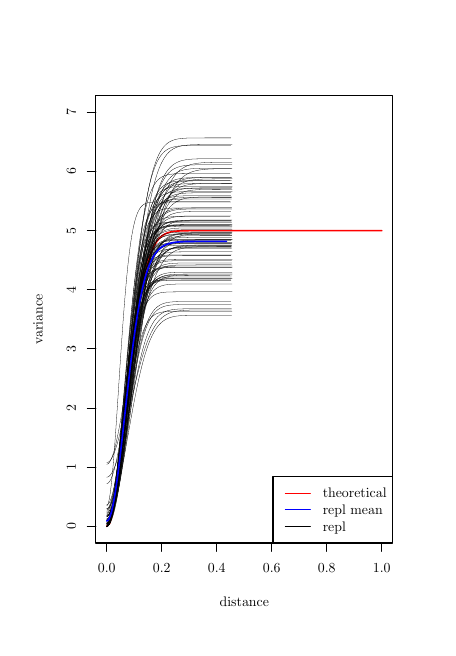
\begin{tikzpicture}[x=1pt,y=1pt]
\definecolor{fillColor}{RGB}{255,255,255}
\path[use as bounding box,fill=fillColor,fill opacity=0.00] (0,0) rectangle (144.54,216.81);
\begin{scope}
\path[clip] ( 24.60, 30.60) rectangle (131.94,192.21);
\definecolor{drawColor}{RGB}{255,0,0}

\path[draw=drawColor,line width= 0.6pt,line join=round,line cap=round] ( 28.58, 36.59) --
	( 29.58, 37.67) --
	( 30.58, 40.86) --
	( 31.59, 45.96) --
	( 32.59, 52.68) --
	( 33.60, 60.65) --
	( 34.60, 69.44) --
	( 35.60, 78.64) --
	( 36.61, 87.84) --
	( 37.61, 96.70) --
	( 38.61,104.94) --
	( 39.62,112.37) --
	( 40.62,118.88) --
	( 41.63,124.41) --
	( 42.63,129.00) --
	( 43.63,132.71) --
	( 44.64,135.63) --
	( 45.64,137.87) --
	( 46.65,139.55) --
	( 47.65,140.78) --
	( 48.65,141.67) --
	( 49.66,142.28) --
	( 50.66,142.70) --
	( 51.67,142.99) --
	( 52.67,143.17) --
	( 53.67,143.29) --
	( 54.68,143.36) --
	( 55.68,143.41) --
	( 56.69,143.43) --
	( 57.69,143.45) --
	( 58.69,143.46) --
	( 59.70,143.46) --
	( 60.70,143.47) --
	( 61.71,143.47) --
	( 62.71,143.47) --
	( 63.71,143.47) --
	( 64.72,143.47) --
	( 65.72,143.47) --
	( 66.72,143.47) --
	( 67.73,143.47) --
	( 68.73,143.47) --
	( 69.74,143.47) --
	( 70.74,143.47) --
	( 71.74,143.47) --
	( 72.75,143.47) --
	( 73.75,143.47) --
	( 74.76,143.47) --
	( 75.76,143.47) --
	( 76.76,143.47) --
	( 77.77,143.47) --
	( 78.77,143.47) --
	( 79.78,143.47) --
	( 80.78,143.47) --
	( 81.78,143.47) --
	( 82.79,143.47) --
	( 83.79,143.47) --
	( 84.80,143.47) --
	( 85.80,143.47) --
	( 86.80,143.47) --
	( 87.81,143.47) --
	( 88.81,143.47) --
	( 89.82,143.47) --
	( 90.82,143.47) --
	( 91.82,143.47) --
	( 92.83,143.47) --
	( 93.83,143.47) --
	( 94.83,143.47) --
	( 95.84,143.47) --
	( 96.84,143.47) --
	( 97.85,143.47) --
	( 98.85,143.47) --
	( 99.85,143.47) --
	(100.86,143.47) --
	(101.86,143.47) --
	(102.87,143.47) --
	(103.87,143.47) --
	(104.87,143.47) --
	(105.88,143.47) --
	(106.88,143.47) --
	(107.89,143.47) --
	(108.89,143.47) --
	(109.89,143.47) --
	(110.90,143.47) --
	(111.90,143.47) --
	(112.91,143.47) --
	(113.91,143.47) --
	(114.91,143.47) --
	(115.92,143.47) --
	(116.92,143.47) --
	(117.93,143.47) --
	(118.93,143.47) --
	(119.93,143.47) --
	(120.94,143.47) --
	(121.94,143.47) --
	(122.94,143.47) --
	(123.95,143.47) --
	(124.95,143.47) --
	(125.96,143.47) --
	(126.96,143.47) --
	(127.96,143.47);
\end{scope}
\begin{scope}
\path[clip] (  0.00,  0.00) rectangle (144.54,216.81);
\definecolor{drawColor}{RGB}{0,0,0}

\path[draw=drawColor,line width= 0.4pt,line join=round,line cap=round] ( 28.58, 30.60) -- (127.96, 30.60);

\path[draw=drawColor,line width= 0.4pt,line join=round,line cap=round] ( 28.58, 30.60) -- ( 28.58, 27.60);

\path[draw=drawColor,line width= 0.4pt,line join=round,line cap=round] ( 48.45, 30.60) -- ( 48.45, 27.60);

\path[draw=drawColor,line width= 0.4pt,line join=round,line cap=round] ( 68.33, 30.60) -- ( 68.33, 27.60);

\path[draw=drawColor,line width= 0.4pt,line join=round,line cap=round] ( 88.21, 30.60) -- ( 88.21, 27.60);

\path[draw=drawColor,line width= 0.4pt,line join=round,line cap=round] (108.09, 30.60) -- (108.09, 27.60);

\path[draw=drawColor,line width= 0.4pt,line join=round,line cap=round] (127.96, 30.60) -- (127.96, 27.60);

\node[text=drawColor,anchor=base,inner sep=0pt, outer sep=0pt, scale=  0.50] at ( 28.58, 19.80) {0.0};

\node[text=drawColor,anchor=base,inner sep=0pt, outer sep=0pt, scale=  0.50] at ( 48.45, 19.80) {0.2};

\node[text=drawColor,anchor=base,inner sep=0pt, outer sep=0pt, scale=  0.50] at ( 68.33, 19.80) {0.4};

\node[text=drawColor,anchor=base,inner sep=0pt, outer sep=0pt, scale=  0.50] at ( 88.21, 19.80) {0.6};

\node[text=drawColor,anchor=base,inner sep=0pt, outer sep=0pt, scale=  0.50] at (108.09, 19.80) {0.8};

\node[text=drawColor,anchor=base,inner sep=0pt, outer sep=0pt, scale=  0.50] at (127.96, 19.80) {1.0};

\path[draw=drawColor,line width= 0.4pt,line join=round,line cap=round] ( 24.60, 36.59) -- ( 24.60,186.22);

\path[draw=drawColor,line width= 0.4pt,line join=round,line cap=round] ( 24.60, 36.59) -- ( 21.60, 36.59);

\path[draw=drawColor,line width= 0.4pt,line join=round,line cap=round] ( 24.60, 57.96) -- ( 21.60, 57.96);

\path[draw=drawColor,line width= 0.4pt,line join=round,line cap=round] ( 24.60, 79.34) -- ( 21.60, 79.34);

\path[draw=drawColor,line width= 0.4pt,line join=round,line cap=round] ( 24.60,100.72) -- ( 21.60,100.72);

\path[draw=drawColor,line width= 0.4pt,line join=round,line cap=round] ( 24.60,122.09) -- ( 21.60,122.09);

\path[draw=drawColor,line width= 0.4pt,line join=round,line cap=round] ( 24.60,143.47) -- ( 21.60,143.47);

\path[draw=drawColor,line width= 0.4pt,line join=round,line cap=round] ( 24.60,164.85) -- ( 21.60,164.85);

\path[draw=drawColor,line width= 0.4pt,line join=round,line cap=round] ( 24.60,186.22) -- ( 21.60,186.22);

\node[text=drawColor,rotate= 90.00,anchor=base,inner sep=0pt, outer sep=0pt, scale=  0.50] at ( 17.40, 36.59) {0};

\node[text=drawColor,rotate= 90.00,anchor=base,inner sep=0pt, outer sep=0pt, scale=  0.50] at ( 17.40, 57.96) {1};

\node[text=drawColor,rotate= 90.00,anchor=base,inner sep=0pt, outer sep=0pt, scale=  0.50] at ( 17.40, 79.34) {2};

\node[text=drawColor,rotate= 90.00,anchor=base,inner sep=0pt, outer sep=0pt, scale=  0.50] at ( 17.40,100.72) {3};

\node[text=drawColor,rotate= 90.00,anchor=base,inner sep=0pt, outer sep=0pt, scale=  0.50] at ( 17.40,122.09) {4};

\node[text=drawColor,rotate= 90.00,anchor=base,inner sep=0pt, outer sep=0pt, scale=  0.50] at ( 17.40,143.47) {5};

\node[text=drawColor,rotate= 90.00,anchor=base,inner sep=0pt, outer sep=0pt, scale=  0.50] at ( 17.40,164.85) {6};

\node[text=drawColor,rotate= 90.00,anchor=base,inner sep=0pt, outer sep=0pt, scale=  0.50] at ( 17.40,186.22) {7};

\path[draw=drawColor,line width= 0.4pt,line join=round,line cap=round] ( 24.60, 30.60) --
	(131.94, 30.60) --
	(131.94,192.21) --
	( 24.60,192.21) --
	( 24.60, 30.60);
\end{scope}
\begin{scope}
\path[clip] (  0.00,  0.00) rectangle (144.54,216.81);
\definecolor{drawColor}{RGB}{0,0,0}

\node[text=drawColor,anchor=base,inner sep=0pt, outer sep=0pt, scale=  0.50] at ( 78.27,  7.80) {distance};

\node[text=drawColor,rotate= 90.00,anchor=base,inner sep=0pt, outer sep=0pt, scale=  0.50] at (  5.40,111.41) {variance};
\end{scope}
\begin{scope}
\path[clip] ( 24.60, 30.60) rectangle (131.94,192.21);
\definecolor{drawColor}{RGB}{0,0,0}

\path[draw=drawColor,line width= 0.1pt,line join=round,line cap=round] ( 28.58, 41.59) --
	( 28.80, 41.62) --
	( 29.03, 41.72) --
	( 29.26, 41.87) --
	( 29.48, 42.09) --
	( 29.71, 42.36) --
	( 29.94, 42.70) --
	( 30.16, 43.09) --
	( 30.39, 43.54) --
	( 30.62, 44.05) --
	( 30.84, 44.62) --
	( 31.07, 45.24) --
	( 31.30, 45.91) --
	( 31.52, 46.63) --
	( 31.75, 47.40) --
	( 31.98, 48.22) --
	( 32.20, 49.08) --
	( 32.43, 49.99) --
	( 32.66, 50.94) --
	( 32.88, 51.92) --
	( 33.11, 52.94) --
	( 33.34, 54.00) --
	( 33.56, 55.09) --
	( 33.79, 56.20) --
	( 34.02, 57.35) --
	( 34.24, 58.52) --
	( 34.47, 59.70) --
	( 34.70, 60.91) --
	( 34.92, 62.14) --
	( 35.15, 63.38) --
	( 35.38, 64.63) --
	( 35.60, 65.89) --
	( 35.83, 67.15) --
	( 36.06, 68.42) --
	( 36.29, 69.70) --
	( 36.51, 70.97) --
	( 36.74, 72.24) --
	( 36.97, 73.51) --
	( 37.19, 74.77) --
	( 37.42, 76.02) --
	( 37.65, 77.26) --
	( 37.87, 78.49) --
	( 38.10, 79.71) --
	( 38.33, 80.91) --
	( 38.55, 82.09) --
	( 38.78, 83.26) --
	( 39.01, 84.41) --
	( 39.23, 85.53) --
	( 39.46, 86.64) --
	( 39.69, 87.72) --
	( 39.91, 88.78) --
	( 40.14, 89.81) --
	( 40.37, 90.82) --
	( 40.59, 91.80) --
	( 40.82, 92.76) --
	( 41.05, 93.69) --
	( 41.27, 94.59) --
	( 41.50, 95.47) --
	( 41.73, 96.32) --
	( 41.95, 97.14) --
	( 42.18, 97.93) --
	( 42.41, 98.70) --
	( 42.63, 99.43) --
	( 42.86,100.14) --
	( 43.09,100.83) --
	( 43.31,101.49) --
	( 43.54,102.12) --
	( 43.77,102.72) --
	( 43.99,103.30) --
	( 44.22,103.86) --
	( 44.45,104.39) --
	( 44.68,104.89) --
	( 44.90,105.37) --
	( 45.13,105.83) --
	( 45.36,106.27) --
	( 45.58,106.69) --
	( 45.81,107.08) --
	( 46.04,107.46) --
	( 46.26,107.81) --
	( 46.49,108.15) --
	( 46.72,108.46) --
	( 46.94,108.76) --
	( 47.17,109.05) --
	( 47.40,109.32) --
	( 47.62,109.57) --
	( 47.85,109.80) --
	( 48.08,110.03) --
	( 48.30,110.23) --
	( 48.53,110.43) --
	( 48.76,110.61) --
	( 48.98,110.79) --
	( 49.21,110.95) --
	( 49.44,111.10) --
	( 49.66,111.24) --
	( 49.89,111.37) --
	( 50.12,111.49) --
	( 50.34,111.60) --
	( 50.57,111.71) --
	( 50.80,111.81) --
	( 51.02,111.90) --
	( 51.25,111.98) --
	( 51.48,112.06) --
	( 51.70,112.13) --
	( 51.93,112.20) --
	( 52.16,112.26) --
	( 52.38,112.32) --
	( 52.61,112.37) --
	( 52.84,112.42) --
	( 53.06,112.46) --
	( 53.29,112.51) --
	( 53.52,112.54) --
	( 53.75,112.58) --
	( 53.97,112.61) --
	( 54.20,112.64) --
	( 54.43,112.66) --
	( 54.65,112.69) --
	( 54.88,112.71) --
	( 55.11,112.73) --
	( 55.33,112.75) --
	( 55.56,112.77) --
	( 55.79,112.78) --
	( 56.01,112.79) --
	( 56.24,112.81) --
	( 56.47,112.82) --
	( 56.69,112.83) --
	( 56.92,112.84) --
	( 57.15,112.85) --
	( 57.37,112.85) --
	( 57.60,112.86) --
	( 57.83,112.87) --
	( 58.05,112.87) --
	( 58.28,112.88) --
	( 58.51,112.88) --
	( 58.73,112.89) --
	( 58.96,112.89) --
	( 59.19,112.89) --
	( 59.41,112.90) --
	( 59.64,112.90) --
	( 59.87,112.90) --
	( 60.09,112.90) --
	( 60.32,112.91) --
	( 60.55,112.91) --
	( 60.77,112.91) --
	( 61.00,112.91) --
	( 61.23,112.91) --
	( 61.45,112.91) --
	( 61.68,112.91) --
	( 61.91,112.91) --
	( 62.14,112.91) --
	( 62.36,112.91) --
	( 62.59,112.92) --
	( 62.82,112.92) --
	( 63.04,112.92) --
	( 63.27,112.92) --
	( 63.50,112.92) --
	( 63.72,112.92) --
	( 63.95,112.92) --
	( 64.18,112.92) --
	( 64.40,112.92) --
	( 64.63,112.92) --
	( 64.86,112.92) --
	( 65.08,112.92) --
	( 65.31,112.92) --
	( 65.54,112.92) --
	( 65.76,112.92) --
	( 65.99,112.92) --
	( 66.22,112.92) --
	( 66.44,112.92) --
	( 66.67,112.92) --
	( 66.90,112.92) --
	( 67.12,112.92) --
	( 67.35,112.92) --
	( 67.58,112.92) --
	( 67.80,112.92) --
	( 68.03,112.92) --
	( 68.26,112.92) --
	( 68.48,112.92) --
	( 68.71,112.92) --
	( 68.94,112.92) --
	( 69.16,112.92) --
	( 69.39,112.92) --
	( 69.62,112.92) --
	( 69.84,112.92) --
	( 70.07,112.92) --
	( 70.30,112.92) --
	( 70.52,112.92) --
	( 70.75,112.92) --
	( 70.98,112.92) --
	( 71.21,112.92) --
	( 71.43,112.92) --
	( 71.66,112.92) --
	( 71.89,112.92) --
	( 72.11,112.92) --
	( 72.34,112.92) --
	( 72.57,112.92) --
	( 72.79,112.92) --
	( 73.02,112.92) --
	( 73.25,112.92) --
	( 73.47,112.92) --
	( 73.70,112.92);

\path[draw=drawColor,line width= 0.1pt,line join=round,line cap=round] ( 28.58, 36.59) --
	( 28.80, 36.65) --
	( 29.03, 36.84) --
	( 29.25, 37.17) --
	( 29.48, 37.61) --
	( 29.71, 38.19) --
	( 29.93, 38.89) --
	( 30.16, 39.70) --
	( 30.39, 40.64) --
	( 30.61, 41.69) --
	( 30.84, 42.85) --
	( 31.07, 44.11) --
	( 31.29, 45.48) --
	( 31.52, 46.94) --
	( 31.75, 48.49) --
	( 31.97, 50.13) --
	( 32.20, 51.85) --
	( 32.43, 53.65) --
	( 32.65, 55.51) --
	( 32.88, 57.43) --
	( 33.10, 59.41) --
	( 33.33, 61.44) --
	( 33.56, 63.51) --
	( 33.78, 65.62) --
	( 34.01, 67.75) --
	( 34.24, 69.92) --
	( 34.46, 72.10) --
	( 34.69, 74.29) --
	( 34.92, 76.48) --
	( 35.14, 78.68) --
	( 35.37, 80.87) --
	( 35.60, 83.05) --
	( 35.82, 85.22) --
	( 36.05, 87.37) --
	( 36.27, 89.49) --
	( 36.50, 91.58) --
	( 36.73, 93.64) --
	( 36.95, 95.66) --
	( 37.18, 97.64) --
	( 37.41, 99.58) --
	( 37.63,101.47) --
	( 37.86,103.32) --
	( 38.09,105.11) --
	( 38.31,106.85) --
	( 38.54,108.54) --
	( 38.77,110.17) --
	( 38.99,111.75) --
	( 39.22,113.27) --
	( 39.45,114.73) --
	( 39.67,116.13) --
	( 39.90,117.48) --
	( 40.12,118.77) --
	( 40.35,120.00) --
	( 40.58,121.18) --
	( 40.80,122.30) --
	( 41.03,123.36) --
	( 41.26,124.38) --
	( 41.48,125.34) --
	( 41.71,126.24) --
	( 41.94,127.10) --
	( 42.16,127.91) --
	( 42.39,128.67) --
	( 42.62,129.39) --
	( 42.84,130.06) --
	( 43.07,130.70) --
	( 43.29,131.29) --
	( 43.52,131.84) --
	( 43.75,132.36) --
	( 43.97,132.84) --
	( 44.20,133.29) --
	( 44.43,133.70) --
	( 44.65,134.09) --
	( 44.88,134.45) --
	( 45.11,134.78) --
	( 45.33,135.08) --
	( 45.56,135.37) --
	( 45.79,135.63) --
	( 46.01,135.87) --
	( 46.24,136.09) --
	( 46.47,136.29) --
	( 46.69,136.47) --
	( 46.92,136.64) --
	( 47.14,136.80) --
	( 47.37,136.94) --
	( 47.60,137.06) --
	( 47.82,137.18) --
	( 48.05,137.29) --
	( 48.28,137.38) --
	( 48.50,137.47) --
	( 48.73,137.55) --
	( 48.96,137.62) --
	( 49.18,137.68) --
	( 49.41,137.74) --
	( 49.64,137.79) --
	( 49.86,137.84) --
	( 50.09,137.88) --
	( 50.32,137.92) --
	( 50.54,137.95) --
	( 50.77,137.98) --
	( 50.99,138.01) --
	( 51.22,138.03) --
	( 51.45,138.05) --
	( 51.67,138.07) --
	( 51.90,138.09) --
	( 52.13,138.10) --
	( 52.35,138.12) --
	( 52.58,138.13) --
	( 52.81,138.14) --
	( 53.03,138.15) --
	( 53.26,138.15) --
	( 53.49,138.16) --
	( 53.71,138.17) --
	( 53.94,138.17) --
	( 54.16,138.18) --
	( 54.39,138.18) --
	( 54.62,138.18) --
	( 54.84,138.19) --
	( 55.07,138.19) --
	( 55.30,138.19) --
	( 55.52,138.19) --
	( 55.75,138.20) --
	( 55.98,138.20) --
	( 56.20,138.20) --
	( 56.43,138.20) --
	( 56.66,138.20) --
	( 56.88,138.20) --
	( 57.11,138.20) --
	( 57.34,138.20) --
	( 57.56,138.20) --
	( 57.79,138.20) --
	( 58.01,138.21) --
	( 58.24,138.21) --
	( 58.47,138.21) --
	( 58.69,138.21) --
	( 58.92,138.21) --
	( 59.15,138.21) --
	( 59.37,138.21) --
	( 59.60,138.21) --
	( 59.83,138.21) --
	( 60.05,138.21) --
	( 60.28,138.21) --
	( 60.51,138.21) --
	( 60.73,138.21) --
	( 60.96,138.21) --
	( 61.18,138.21) --
	( 61.41,138.21) --
	( 61.64,138.21) --
	( 61.86,138.21) --
	( 62.09,138.21) --
	( 62.32,138.21) --
	( 62.54,138.21) --
	( 62.77,138.21) --
	( 63.00,138.21) --
	( 63.22,138.21) --
	( 63.45,138.21) --
	( 63.68,138.21) --
	( 63.90,138.21) --
	( 64.13,138.21) --
	( 64.36,138.21) --
	( 64.58,138.21) --
	( 64.81,138.21) --
	( 65.03,138.21) --
	( 65.26,138.21) --
	( 65.49,138.21) --
	( 65.71,138.21) --
	( 65.94,138.21) --
	( 66.17,138.21) --
	( 66.39,138.21) --
	( 66.62,138.21) --
	( 66.85,138.21) --
	( 67.07,138.21) --
	( 67.30,138.21) --
	( 67.53,138.21) --
	( 67.75,138.21) --
	( 67.98,138.21) --
	( 68.20,138.21) --
	( 68.43,138.21) --
	( 68.66,138.21) --
	( 68.88,138.21) --
	( 69.11,138.21) --
	( 69.34,138.21) --
	( 69.56,138.21) --
	( 69.79,138.21) --
	( 70.02,138.21) --
	( 70.24,138.21) --
	( 70.47,138.21) --
	( 70.70,138.21) --
	( 70.92,138.21) --
	( 71.15,138.21) --
	( 71.38,138.21) --
	( 71.60,138.21) --
	( 71.83,138.21) --
	( 72.05,138.21) --
	( 72.28,138.21) --
	( 72.51,138.21) --
	( 72.73,138.21) --
	( 72.96,138.21) --
	( 73.19,138.21) --
	( 73.41,138.21) --
	( 73.64,138.21);

\path[draw=drawColor,line width= 0.1pt,line join=round,line cap=round] ( 28.58, 36.97) --
	( 28.80, 37.03) --
	( 29.03, 37.21) --
	( 29.26, 37.51) --
	( 29.48, 37.92) --
	( 29.71, 38.46) --
	( 29.94, 39.10) --
	( 30.16, 39.86) --
	( 30.39, 40.73) --
	( 30.62, 41.71) --
	( 30.84, 42.79) --
	( 31.07, 43.98) --
	( 31.30, 45.26) --
	( 31.52, 46.63) --
	( 31.75, 48.09) --
	( 31.98, 49.64) --
	( 32.20, 51.26) --
	( 32.43, 52.96) --
	( 32.66, 54.72) --
	( 32.88, 56.56) --
	( 33.11, 58.45) --
	( 33.34, 60.39) --
	( 33.56, 62.38) --
	( 33.79, 64.41) --
	( 34.02, 66.48) --
	( 34.24, 68.58) --
	( 34.47, 70.71) --
	( 34.70, 72.85) --
	( 34.92, 75.02) --
	( 35.15, 77.19) --
	( 35.38, 79.36) --
	( 35.60, 81.54) --
	( 35.83, 83.71) --
	( 36.06, 85.87) --
	( 36.29, 88.02) --
	( 36.51, 90.15) --
	( 36.74, 92.25) --
	( 36.97, 94.33) --
	( 37.19, 96.39) --
	( 37.42, 98.40) --
	( 37.65,100.39) --
	( 37.87,102.33) --
	( 38.10,104.24) --
	( 38.33,106.10) --
	( 38.55,107.91) --
	( 38.78,109.68) --
	( 39.01,111.40) --
	( 39.23,113.07) --
	( 39.46,114.69) --
	( 39.69,116.25) --
	( 39.91,117.77) --
	( 40.14,119.23) --
	( 40.37,120.63) --
	( 40.59,121.99) --
	( 40.82,123.29) --
	( 41.05,124.54) --
	( 41.27,125.73) --
	( 41.50,126.87) --
	( 41.73,127.96) --
	( 41.95,129.00) --
	( 42.18,130.00) --
	( 42.41,130.94) --
	( 42.63,131.83) --
	( 42.86,132.68) --
	( 43.09,133.49) --
	( 43.31,134.25) --
	( 43.54,134.97) --
	( 43.77,135.64) --
	( 43.99,136.28) --
	( 44.22,136.88) --
	( 44.45,137.45) --
	( 44.67,137.98) --
	( 44.90,138.47) --
	( 45.13,138.94) --
	( 45.36,139.37) --
	( 45.58,139.77) --
	( 45.81,140.15) --
	( 46.04,140.50) --
	( 46.26,140.83) --
	( 46.49,141.13) --
	( 46.72,141.41) --
	( 46.94,141.67) --
	( 47.17,141.92) --
	( 47.40,142.14) --
	( 47.62,142.34) --
	( 47.85,142.53) --
	( 48.08,142.71) --
	( 48.30,142.87) --
	( 48.53,143.01) --
	( 48.76,143.15) --
	( 48.98,143.27) --
	( 49.21,143.39) --
	( 49.44,143.49) --
	( 49.66,143.58) --
	( 49.89,143.67) --
	( 50.12,143.75) --
	( 50.34,143.82) --
	( 50.57,143.88) --
	( 50.80,143.94) --
	( 51.02,143.99) --
	( 51.25,144.04) --
	( 51.48,144.08) --
	( 51.70,144.12) --
	( 51.93,144.16) --
	( 52.16,144.19) --
	( 52.38,144.22) --
	( 52.61,144.24) --
	( 52.84,144.27) --
	( 53.06,144.29) --
	( 53.29,144.31) --
	( 53.52,144.32) --
	( 53.74,144.34) --
	( 53.97,144.35) --
	( 54.20,144.36) --
	( 54.43,144.37) --
	( 54.65,144.38) --
	( 54.88,144.39) --
	( 55.11,144.40) --
	( 55.33,144.40) --
	( 55.56,144.41) --
	( 55.79,144.41) --
	( 56.01,144.42) --
	( 56.24,144.42) --
	( 56.47,144.43) --
	( 56.69,144.43) --
	( 56.92,144.43) --
	( 57.15,144.43) --
	( 57.37,144.44) --
	( 57.60,144.44) --
	( 57.83,144.44) --
	( 58.05,144.44) --
	( 58.28,144.44) --
	( 58.51,144.44) --
	( 58.73,144.44) --
	( 58.96,144.44) --
	( 59.19,144.45) --
	( 59.41,144.45) --
	( 59.64,144.45) --
	( 59.87,144.45) --
	( 60.09,144.45) --
	( 60.32,144.45) --
	( 60.55,144.45) --
	( 60.77,144.45) --
	( 61.00,144.45) --
	( 61.23,144.45) --
	( 61.45,144.45) --
	( 61.68,144.45) --
	( 61.91,144.45) --
	( 62.13,144.45) --
	( 62.36,144.45) --
	( 62.59,144.45) --
	( 62.81,144.45) --
	( 63.04,144.45) --
	( 63.27,144.45) --
	( 63.50,144.45) --
	( 63.72,144.45) --
	( 63.95,144.45) --
	( 64.18,144.45) --
	( 64.40,144.45) --
	( 64.63,144.45) --
	( 64.86,144.45) --
	( 65.08,144.45) --
	( 65.31,144.45) --
	( 65.54,144.45) --
	( 65.76,144.45) --
	( 65.99,144.45) --
	( 66.22,144.45) --
	( 66.44,144.45) --
	( 66.67,144.45) --
	( 66.90,144.45) --
	( 67.12,144.45) --
	( 67.35,144.45) --
	( 67.58,144.45) --
	( 67.80,144.45) --
	( 68.03,144.45) --
	( 68.26,144.45) --
	( 68.48,144.45) --
	( 68.71,144.45) --
	( 68.94,144.45) --
	( 69.16,144.45) --
	( 69.39,144.45) --
	( 69.62,144.45) --
	( 69.84,144.45) --
	( 70.07,144.45) --
	( 70.30,144.45) --
	( 70.52,144.45) --
	( 70.75,144.45) --
	( 70.98,144.45) --
	( 71.20,144.45) --
	( 71.43,144.45) --
	( 71.66,144.45) --
	( 71.88,144.45) --
	( 72.11,144.45) --
	( 72.34,144.45) --
	( 72.57,144.45) --
	( 72.79,144.45) --
	( 73.02,144.45) --
	( 73.25,144.45) --
	( 73.47,144.45) --
	( 73.70,144.45);

\path[draw=drawColor,line width= 0.1pt,line join=round,line cap=round] ( 28.58, 36.59) --
	( 28.80, 36.65) --
	( 29.03, 36.82) --
	( 29.25, 37.12) --
	( 29.48, 37.54) --
	( 29.70, 38.07) --
	( 29.93, 38.72) --
	( 30.15, 39.48) --
	( 30.38, 40.36) --
	( 30.60, 41.34) --
	( 30.83, 42.43) --
	( 31.05, 43.62) --
	( 31.28, 44.91) --
	( 31.51, 46.29) --
	( 31.73, 47.77) --
	( 31.96, 49.33) --
	( 32.18, 50.98) --
	( 32.41, 52.70) --
	( 32.63, 54.50) --
	( 32.86, 56.36) --
	( 33.08, 58.29) --
	( 33.31, 60.28) --
	( 33.53, 62.33) --
	( 33.76, 64.42) --
	( 33.98, 66.55) --
	( 34.21, 68.72) --
	( 34.43, 70.93) --
	( 34.66, 73.16) --
	( 34.89, 75.41) --
	( 35.11, 77.69) --
	( 35.34, 79.97) --
	( 35.56, 82.26) --
	( 35.79, 84.56) --
	( 36.01, 86.85) --
	( 36.24, 89.14) --
	( 36.46, 91.41) --
	( 36.69, 93.67) --
	( 36.91, 95.92) --
	( 37.14, 98.14) --
	( 37.36,100.33) --
	( 37.59,102.49) --
	( 37.82,104.63) --
	( 38.04,106.72) --
	( 38.27,108.78) --
	( 38.49,110.80) --
	( 38.72,112.78) --
	( 38.94,114.71) --
	( 39.17,116.59) --
	( 39.39,118.43) --
	( 39.62,120.22) --
	( 39.84,121.95) --
	( 40.07,123.64) --
	( 40.29,125.27) --
	( 40.52,126.85) --
	( 40.74,128.38) --
	( 40.97,129.85) --
	( 41.20,131.27) --
	( 41.42,132.64) --
	( 41.65,133.95) --
	( 41.87,135.21) --
	( 42.10,136.42) --
	( 42.32,137.58) --
	( 42.55,138.68) --
	( 42.77,139.74) --
	( 43.00,140.75) --
	( 43.22,141.71) --
	( 43.45,142.62) --
	( 43.67,143.49) --
	( 43.90,144.32) --
	( 44.13,145.10) --
	( 44.35,145.84) --
	( 44.58,146.54) --
	( 44.80,147.20) --
	( 45.03,147.82) --
	( 45.25,148.41) --
	( 45.48,148.96) --
	( 45.70,149.48) --
	( 45.93,149.97) --
	( 46.15,150.43) --
	( 46.38,150.86) --
	( 46.60,151.26) --
	( 46.83,151.63) --
	( 47.05,151.98) --
	( 47.28,152.31) --
	( 47.51,152.61) --
	( 47.73,152.89) --
	( 47.96,153.16) --
	( 48.18,153.40) --
	( 48.41,153.63) --
	( 48.63,153.84) --
	( 48.86,154.03) --
	( 49.08,154.21) --
	( 49.31,154.37) --
	( 49.53,154.52) --
	( 49.76,154.67) --
	( 49.98,154.79) --
	( 50.21,154.91) --
	( 50.44,155.02) --
	( 50.66,155.12) --
	( 50.89,155.21) --
	( 51.11,155.30) --
	( 51.34,155.37) --
	( 51.56,155.44) --
	( 51.79,155.50) --
	( 52.01,155.56) --
	( 52.24,155.62) --
	( 52.46,155.66) --
	( 52.69,155.71) --
	( 52.91,155.75) --
	( 53.14,155.78) --
	( 53.36,155.81) --
	( 53.59,155.84) --
	( 53.82,155.87) --
	( 54.04,155.89) --
	( 54.27,155.91) --
	( 54.49,155.93) --
	( 54.72,155.95) --
	( 54.94,155.97) --
	( 55.17,155.98) --
	( 55.39,155.99) --
	( 55.62,156.00) --
	( 55.84,156.01) --
	( 56.07,156.02) --
	( 56.29,156.03) --
	( 56.52,156.04) --
	( 56.75,156.04) --
	( 56.97,156.05) --
	( 57.20,156.05) --
	( 57.42,156.06) --
	( 57.65,156.06) --
	( 57.87,156.07) --
	( 58.10,156.07) --
	( 58.32,156.07) --
	( 58.55,156.07) --
	( 58.77,156.08) --
	( 59.00,156.08) --
	( 59.22,156.08) --
	( 59.45,156.08) --
	( 59.67,156.08) --
	( 59.90,156.08) --
	( 60.13,156.08) --
	( 60.35,156.09) --
	( 60.58,156.09) --
	( 60.80,156.09) --
	( 61.03,156.09) --
	( 61.25,156.09) --
	( 61.48,156.09) --
	( 61.70,156.09) --
	( 61.93,156.09) --
	( 62.15,156.09) --
	( 62.38,156.09) --
	( 62.60,156.09) --
	( 62.83,156.09) --
	( 63.06,156.09) --
	( 63.28,156.09) --
	( 63.51,156.09) --
	( 63.73,156.09) --
	( 63.96,156.09) --
	( 64.18,156.09) --
	( 64.41,156.09) --
	( 64.63,156.09) --
	( 64.86,156.09) --
	( 65.08,156.09) --
	( 65.31,156.09) --
	( 65.53,156.09) --
	( 65.76,156.09) --
	( 65.98,156.09) --
	( 66.21,156.09) --
	( 66.44,156.09) --
	( 66.66,156.09) --
	( 66.89,156.09) --
	( 67.11,156.09) --
	( 67.34,156.09) --
	( 67.56,156.09) --
	( 67.79,156.09) --
	( 68.01,156.09) --
	( 68.24,156.09) --
	( 68.46,156.09) --
	( 68.69,156.09) --
	( 68.91,156.09) --
	( 69.14,156.09) --
	( 69.37,156.09) --
	( 69.59,156.09) --
	( 69.82,156.09) --
	( 70.04,156.09) --
	( 70.27,156.09) --
	( 70.49,156.09) --
	( 70.72,156.09) --
	( 70.94,156.09) --
	( 71.17,156.09) --
	( 71.39,156.09) --
	( 71.62,156.09) --
	( 71.84,156.09) --
	( 72.07,156.09) --
	( 72.29,156.09) --
	( 72.52,156.09) --
	( 72.75,156.09) --
	( 72.97,156.09) --
	( 73.20,156.09) --
	( 73.42,156.09);

\path[draw=drawColor,line width= 0.1pt,line join=round,line cap=round] ( 28.58, 36.59) --
	( 28.80, 36.65) --
	( 29.03, 36.86) --
	( 29.25, 37.20) --
	( 29.48, 37.67) --
	( 29.70, 38.27) --
	( 29.93, 39.00) --
	( 30.15, 39.86) --
	( 30.38, 40.84) --
	( 30.61, 41.93) --
	( 30.83, 43.14) --
	( 31.06, 44.45) --
	( 31.28, 45.87) --
	( 31.51, 47.38) --
	( 31.73, 48.98) --
	( 31.96, 50.66) --
	( 32.19, 52.41) --
	( 32.41, 54.24) --
	( 32.64, 56.12) --
	( 32.86, 58.06) --
	( 33.09, 60.04) --
	( 33.31, 62.07) --
	( 33.54, 64.12) --
	( 33.76, 66.20) --
	( 33.99, 68.30) --
	( 34.22, 70.41) --
	( 34.44, 72.52) --
	( 34.67, 74.63) --
	( 34.89, 76.73) --
	( 35.12, 78.81) --
	( 35.34, 80.87) --
	( 35.57, 82.91) --
	( 35.80, 84.92) --
	( 36.02, 86.89) --
	( 36.25, 88.82) --
	( 36.47, 90.71) --
	( 36.70, 92.56) --
	( 36.92, 94.35) --
	( 37.15, 96.09) --
	( 37.37, 97.78) --
	( 37.60, 99.41) --
	( 37.83,100.98) --
	( 38.05,102.49) --
	( 38.28,103.95) --
	( 38.50,105.34) --
	( 38.73,106.67) --
	( 38.95,107.94) --
	( 39.18,109.15) --
	( 39.41,110.31) --
	( 39.63,111.40) --
	( 39.86,112.43) --
	( 40.08,113.41) --
	( 40.31,114.33) --
	( 40.53,115.20) --
	( 40.76,116.01) --
	( 40.98,116.78) --
	( 41.21,117.50) --
	( 41.44,118.17) --
	( 41.66,118.79) --
	( 41.89,119.37) --
	( 42.11,119.91) --
	( 42.34,120.41) --
	( 42.56,120.88) --
	( 42.79,121.30) --
	( 43.02,121.70) --
	( 43.24,122.06) --
	( 43.47,122.40) --
	( 43.69,122.71) --
	( 43.92,122.99) --
	( 44.14,123.25) --
	( 44.37,123.48) --
	( 44.59,123.70) --
	( 44.82,123.89) --
	( 45.05,124.07) --
	( 45.27,124.23) --
	( 45.50,124.37) --
	( 45.72,124.50) --
	( 45.95,124.62) --
	( 46.17,124.73) --
	( 46.40,124.83) --
	( 46.63,124.91) --
	( 46.85,124.99) --
	( 47.08,125.06) --
	( 47.30,125.12) --
	( 47.53,125.17) --
	( 47.75,125.22) --
	( 47.98,125.27) --
	( 48.20,125.30) --
	( 48.43,125.34) --
	( 48.66,125.37) --
	( 48.88,125.40) --
	( 49.11,125.42) --
	( 49.33,125.44) --
	( 49.56,125.46) --
	( 49.78,125.47) --
	( 50.01,125.49) --
	( 50.24,125.50) --
	( 50.46,125.51) --
	( 50.69,125.52) --
	( 50.91,125.53) --
	( 51.14,125.53) --
	( 51.36,125.54) --
	( 51.59,125.55) --
	( 51.81,125.55) --
	( 52.04,125.55) --
	( 52.27,125.56) --
	( 52.49,125.56) --
	( 52.72,125.56) --
	( 52.94,125.57) --
	( 53.17,125.57) --
	( 53.39,125.57) --
	( 53.62,125.57) --
	( 53.85,125.57) --
	( 54.07,125.57) --
	( 54.30,125.57) --
	( 54.52,125.57) --
	( 54.75,125.57) --
	( 54.97,125.57) --
	( 55.20,125.57) --
	( 55.42,125.58) --
	( 55.65,125.58) --
	( 55.88,125.58) --
	( 56.10,125.58) --
	( 56.33,125.58) --
	( 56.55,125.58) --
	( 56.78,125.58) --
	( 57.00,125.58) --
	( 57.23,125.58) --
	( 57.46,125.58) --
	( 57.68,125.58) --
	( 57.91,125.58) --
	( 58.13,125.58) --
	( 58.36,125.58) --
	( 58.58,125.58) --
	( 58.81,125.58) --
	( 59.03,125.58) --
	( 59.26,125.58) --
	( 59.49,125.58) --
	( 59.71,125.58) --
	( 59.94,125.58) --
	( 60.16,125.58) --
	( 60.39,125.58) --
	( 60.61,125.58) --
	( 60.84,125.58) --
	( 61.07,125.58) --
	( 61.29,125.58) --
	( 61.52,125.58) --
	( 61.74,125.58) --
	( 61.97,125.58) --
	( 62.19,125.58) --
	( 62.42,125.58) --
	( 62.64,125.58) --
	( 62.87,125.58) --
	( 63.10,125.58) --
	( 63.32,125.58) --
	( 63.55,125.58) --
	( 63.77,125.58) --
	( 64.00,125.58) --
	( 64.22,125.58) --
	( 64.45,125.58) --
	( 64.68,125.58) --
	( 64.90,125.58) --
	( 65.13,125.58) --
	( 65.35,125.58) --
	( 65.58,125.58) --
	( 65.80,125.58) --
	( 66.03,125.58) --
	( 66.25,125.58) --
	( 66.48,125.58) --
	( 66.71,125.58) --
	( 66.93,125.58) --
	( 67.16,125.58) --
	( 67.38,125.58) --
	( 67.61,125.58) --
	( 67.83,125.58) --
	( 68.06,125.58) --
	( 68.29,125.58) --
	( 68.51,125.58) --
	( 68.74,125.58) --
	( 68.96,125.58) --
	( 69.19,125.58) --
	( 69.41,125.58) --
	( 69.64,125.58) --
	( 69.86,125.58) --
	( 70.09,125.58) --
	( 70.32,125.58) --
	( 70.54,125.58) --
	( 70.77,125.58) --
	( 70.99,125.58) --
	( 71.22,125.58) --
	( 71.44,125.58) --
	( 71.67,125.58) --
	( 71.90,125.58) --
	( 72.12,125.58) --
	( 72.35,125.58) --
	( 72.57,125.58) --
	( 72.80,125.58) --
	( 73.02,125.58) --
	( 73.25,125.58) --
	( 73.47,125.58);

\path[draw=drawColor,line width= 0.1pt,line join=round,line cap=round] ( 28.58, 36.59) --
	( 28.80, 36.66) --
	( 29.03, 36.87) --
	( 29.26, 37.22) --
	( 29.49, 37.71) --
	( 29.71, 38.33) --
	( 29.94, 39.10) --
	( 30.17, 39.99) --
	( 30.40, 41.01) --
	( 30.63, 42.16) --
	( 30.85, 43.43) --
	( 31.08, 44.82) --
	( 31.31, 46.32) --
	( 31.54, 47.93) --
	( 31.76, 49.64) --
	( 31.99, 51.44) --
	( 32.22, 53.34) --
	( 32.45, 55.33) --
	( 32.67, 57.39) --
	( 32.90, 59.52) --
	( 33.13, 61.73) --
	( 33.36, 63.99) --
	( 33.59, 66.30) --
	( 33.81, 68.66) --
	( 34.04, 71.06) --
	( 34.27, 73.50) --
	( 34.50, 75.96) --
	( 34.72, 78.44) --
	( 34.95, 80.93) --
	( 35.18, 83.43) --
	( 35.41, 85.94) --
	( 35.64, 88.43) --
	( 35.86, 90.92) --
	( 36.09, 93.40) --
	( 36.32, 95.85) --
	( 36.55, 98.28) --
	( 36.77,100.68) --
	( 37.00,103.05) --
	( 37.23,105.38) --
	( 37.46,107.67) --
	( 37.68,109.91) --
	( 37.91,112.10) --
	( 38.14,114.25) --
	( 38.37,116.34) --
	( 38.60,118.37) --
	( 38.82,120.35) --
	( 39.05,122.27) --
	( 39.28,124.13) --
	( 39.51,125.93) --
	( 39.73,127.67) --
	( 39.96,129.34) --
	( 40.19,130.95) --
	( 40.42,132.50) --
	( 40.64,133.98) --
	( 40.87,135.40) --
	( 41.10,136.77) --
	( 41.33,138.06) --
	( 41.56,139.30) --
	( 41.78,140.49) --
	( 42.01,141.61) --
	( 42.24,142.67) --
	( 42.47,143.68) --
	( 42.69,144.64) --
	( 42.92,145.55) --
	( 43.15,146.40) --
	( 43.38,147.21) --
	( 43.61,147.96) --
	( 43.83,148.68) --
	( 44.06,149.34) --
	( 44.29,149.97) --
	( 44.52,150.56) --
	( 44.74,151.11) --
	( 44.97,151.62) --
	( 45.20,152.10) --
	( 45.43,152.54) --
	( 45.65,152.96) --
	( 45.88,153.34) --
	( 46.11,153.70) --
	( 46.34,154.03) --
	( 46.57,154.33) --
	( 46.79,154.62) --
	( 47.02,154.88) --
	( 47.25,155.12) --
	( 47.48,155.34) --
	( 47.70,155.54) --
	( 47.93,155.72) --
	( 48.16,155.90) --
	( 48.39,156.05) --
	( 48.62,156.19) --
	( 48.84,156.32) --
	( 49.07,156.44) --
	( 49.30,156.55) --
	( 49.53,156.65) --
	( 49.75,156.74) --
	( 49.98,156.82) --
	( 50.21,156.89) --
	( 50.44,156.96) --
	( 50.66,157.02) --
	( 50.89,157.07) --
	( 51.12,157.12) --
	( 51.35,157.16) --
	( 51.58,157.20) --
	( 51.80,157.24) --
	( 52.03,157.27) --
	( 52.26,157.30) --
	( 52.49,157.32) --
	( 52.71,157.35) --
	( 52.94,157.37) --
	( 53.17,157.39) --
	( 53.40,157.40) --
	( 53.63,157.42) --
	( 53.85,157.43) --
	( 54.08,157.44) --
	( 54.31,157.45) --
	( 54.54,157.46) --
	( 54.76,157.47) --
	( 54.99,157.47) --
	( 55.22,157.48) --
	( 55.45,157.49) --
	( 55.67,157.49) --
	( 55.90,157.49) --
	( 56.13,157.50) --
	( 56.36,157.50) --
	( 56.59,157.50) --
	( 56.81,157.51) --
	( 57.04,157.51) --
	( 57.27,157.51) --
	( 57.50,157.51) --
	( 57.72,157.51) --
	( 57.95,157.51) --
	( 58.18,157.51) --
	( 58.41,157.52) --
	( 58.64,157.52) --
	( 58.86,157.52) --
	( 59.09,157.52) --
	( 59.32,157.52) --
	( 59.55,157.52) --
	( 59.77,157.52) --
	( 60.00,157.52) --
	( 60.23,157.52) --
	( 60.46,157.52) --
	( 60.68,157.52) --
	( 60.91,157.52) --
	( 61.14,157.52) --
	( 61.37,157.52) --
	( 61.60,157.52) --
	( 61.82,157.52) --
	( 62.05,157.52) --
	( 62.28,157.52) --
	( 62.51,157.52) --
	( 62.73,157.52) --
	( 62.96,157.52) --
	( 63.19,157.52) --
	( 63.42,157.52) --
	( 63.64,157.52) --
	( 63.87,157.52) --
	( 64.10,157.52) --
	( 64.33,157.52) --
	( 64.56,157.52) --
	( 64.78,157.52) --
	( 65.01,157.52) --
	( 65.24,157.52) --
	( 65.47,157.52) --
	( 65.69,157.52) --
	( 65.92,157.52) --
	( 66.15,157.52) --
	( 66.38,157.52) --
	( 66.61,157.52) --
	( 66.83,157.52) --
	( 67.06,157.52) --
	( 67.29,157.52) --
	( 67.52,157.52) --
	( 67.74,157.52) --
	( 67.97,157.52) --
	( 68.20,157.52) --
	( 68.43,157.52) --
	( 68.65,157.52) --
	( 68.88,157.52) --
	( 69.11,157.52) --
	( 69.34,157.52) --
	( 69.57,157.52) --
	( 69.79,157.52) --
	( 70.02,157.52) --
	( 70.25,157.52) --
	( 70.48,157.52) --
	( 70.70,157.52) --
	( 70.93,157.52) --
	( 71.16,157.52) --
	( 71.39,157.52) --
	( 71.62,157.52) --
	( 71.84,157.52) --
	( 72.07,157.52) --
	( 72.30,157.52) --
	( 72.53,157.52) --
	( 72.75,157.52) --
	( 72.98,157.52) --
	( 73.21,157.52) --
	( 73.44,157.52) --
	( 73.66,157.52) --
	( 73.89,157.52);

\path[draw=drawColor,line width= 0.1pt,line join=round,line cap=round] ( 28.58, 54.39) --
	( 28.80, 54.41) --
	( 29.03, 54.48) --
	( 29.25, 54.60) --
	( 29.48, 54.77) --
	( 29.71, 54.98) --
	( 29.93, 55.24) --
	( 30.16, 55.55) --
	( 30.39, 55.90) --
	( 30.61, 56.30) --
	( 30.84, 56.73) --
	( 31.07, 57.21) --
	( 31.29, 57.74) --
	( 31.52, 58.30) --
	( 31.75, 58.90) --
	( 31.97, 59.54) --
	( 32.20, 60.21) --
	( 32.42, 60.92) --
	( 32.65, 61.66) --
	( 32.88, 62.43) --
	( 33.10, 63.24) --
	( 33.33, 64.07) --
	( 33.56, 64.92) --
	( 33.78, 65.80) --
	( 34.01, 66.71) --
	( 34.24, 67.63) --
	( 34.46, 68.57) --
	( 34.69, 69.53) --
	( 34.91, 70.51) --
	( 35.14, 71.49) --
	( 35.37, 72.49) --
	( 35.59, 73.50) --
	( 35.82, 74.52) --
	( 36.05, 75.54) --
	( 36.27, 76.57) --
	( 36.50, 77.60) --
	( 36.73, 78.63) --
	( 36.95, 79.66) --
	( 37.18, 80.69) --
	( 37.40, 81.71) --
	( 37.63, 82.73) --
	( 37.86, 83.75) --
	( 38.08, 84.75) --
	( 38.31, 85.74) --
	( 38.54, 86.73) --
	( 38.76, 87.70) --
	( 38.99, 88.66) --
	( 39.22, 89.60) --
	( 39.44, 90.53) --
	( 39.67, 91.45) --
	( 39.90, 92.34) --
	( 40.12, 93.22) --
	( 40.35, 94.09) --
	( 40.57, 94.93) --
	( 40.80, 95.75) --
	( 41.03, 96.56) --
	( 41.25, 97.34) --
	( 41.48, 98.11) --
	( 41.71, 98.85) --
	( 41.93, 99.57) --
	( 42.16,100.27) --
	( 42.39,100.95) --
	( 42.61,101.61) --
	( 42.84,102.25) --
	( 43.06,102.86) --
	( 43.29,103.46) --
	( 43.52,104.03) --
	( 43.74,104.58) --
	( 43.97,105.12) --
	( 44.20,105.63) --
	( 44.42,106.12) --
	( 44.65,106.59) --
	( 44.88,107.04) --
	( 45.10,107.48) --
	( 45.33,107.89) --
	( 45.56,108.29) --
	( 45.78,108.66) --
	( 46.01,109.03) --
	( 46.23,109.37) --
	( 46.46,109.70) --
	( 46.69,110.01) --
	( 46.91,110.30) --
	( 47.14,110.59) --
	( 47.37,110.85) --
	( 47.59,111.11) --
	( 47.82,111.35) --
	( 48.05,111.57) --
	( 48.27,111.79) --
	( 48.50,111.99) --
	( 48.72,112.18) --
	( 48.95,112.36) --
	( 49.18,112.53) --
	( 49.40,112.69) --
	( 49.63,112.84) --
	( 49.86,112.98) --
	( 50.08,113.11) --
	( 50.31,113.23) --
	( 50.54,113.35) --
	( 50.76,113.46) --
	( 50.99,113.56) --
	( 51.21,113.65) --
	( 51.44,113.74) --
	( 51.67,113.82) --
	( 51.89,113.90) --
	( 52.12,113.97) --
	( 52.35,114.04) --
	( 52.57,114.10) --
	( 52.80,114.16) --
	( 53.03,114.21) --
	( 53.25,114.26) --
	( 53.48,114.30) --
	( 53.71,114.35) --
	( 53.93,114.39) --
	( 54.16,114.42) --
	( 54.38,114.45) --
	( 54.61,114.48) --
	( 54.84,114.51) --
	( 55.06,114.54) --
	( 55.29,114.56) --
	( 55.52,114.58) --
	( 55.74,114.60) --
	( 55.97,114.62) --
	( 56.20,114.64) --
	( 56.42,114.66) --
	( 56.65,114.67) --
	( 56.87,114.68) --
	( 57.10,114.69) --
	( 57.33,114.70) --
	( 57.55,114.71) --
	( 57.78,114.72) --
	( 58.01,114.73) --
	( 58.23,114.74) --
	( 58.46,114.75) --
	( 58.69,114.75) --
	( 58.91,114.76) --
	( 59.14,114.76) --
	( 59.37,114.77) --
	( 59.59,114.77) --
	( 59.82,114.77) --
	( 60.04,114.78) --
	( 60.27,114.78) --
	( 60.50,114.78) --
	( 60.72,114.79) --
	( 60.95,114.79) --
	( 61.18,114.79) --
	( 61.40,114.79) --
	( 61.63,114.79) --
	( 61.86,114.80) --
	( 62.08,114.80) --
	( 62.31,114.80) --
	( 62.53,114.80) --
	( 62.76,114.80) --
	( 62.99,114.80) --
	( 63.21,114.80) --
	( 63.44,114.80) --
	( 63.67,114.80) --
	( 63.89,114.80) --
	( 64.12,114.80) --
	( 64.35,114.80) --
	( 64.57,114.80) --
	( 64.80,114.80) --
	( 65.02,114.80) --
	( 65.25,114.80) --
	( 65.48,114.81) --
	( 65.70,114.81) --
	( 65.93,114.81) --
	( 66.16,114.81) --
	( 66.38,114.81) --
	( 66.61,114.81) --
	( 66.84,114.81) --
	( 67.06,114.81) --
	( 67.29,114.81) --
	( 67.52,114.81) --
	( 67.74,114.81) --
	( 67.97,114.81) --
	( 68.19,114.81) --
	( 68.42,114.81) --
	( 68.65,114.81) --
	( 68.87,114.81) --
	( 69.10,114.81) --
	( 69.33,114.81) --
	( 69.55,114.81) --
	( 69.78,114.81) --
	( 70.01,114.81) --
	( 70.23,114.81) --
	( 70.46,114.81) --
	( 70.68,114.81) --
	( 70.91,114.81) --
	( 71.14,114.81) --
	( 71.36,114.81) --
	( 71.59,114.81) --
	( 71.82,114.81) --
	( 72.04,114.81) --
	( 72.27,114.81) --
	( 72.50,114.81) --
	( 72.72,114.81) --
	( 72.95,114.81) --
	( 73.17,114.81) --
	( 73.40,114.81) --
	( 73.63,114.81);

\path[draw=drawColor,line width= 0.1pt,line join=round,line cap=round] ( 28.58, 39.01) --
	( 28.80, 39.05) --
	( 29.03, 39.19) --
	( 29.26, 39.41) --
	( 29.48, 39.73) --
	( 29.71, 40.13) --
	( 29.93, 40.62) --
	( 30.16, 41.20) --
	( 30.39, 41.86) --
	( 30.61, 42.61) --
	( 30.84, 43.43) --
	( 31.07, 44.34) --
	( 31.29, 45.32) --
	( 31.52, 46.38) --
	( 31.75, 47.50) --
	( 31.97, 48.70) --
	( 32.20, 49.96) --
	( 32.43, 51.29) --
	( 32.65, 52.68) --
	( 32.88, 54.12) --
	( 33.11, 55.61) --
	( 33.33, 57.16) --
	( 33.56, 58.75) --
	( 33.78, 60.38) --
	( 34.01, 62.05) --
	( 34.24, 63.75) --
	( 34.46, 65.49) --
	( 34.69, 67.26) --
	( 34.92, 69.05) --
	( 35.14, 70.85) --
	( 35.37, 72.68) --
	( 35.60, 74.52) --
	( 35.82, 76.37) --
	( 36.05, 78.22) --
	( 36.28, 80.08) --
	( 36.50, 81.94) --
	( 36.73, 83.79) --
	( 36.96, 85.64) --
	( 37.18, 87.47) --
	( 37.41, 89.30) --
	( 37.64, 91.11) --
	( 37.86, 92.90) --
	( 38.09, 94.67) --
	( 38.31, 96.42) --
	( 38.54, 98.14) --
	( 38.77, 99.84) --
	( 38.99,101.51) --
	( 39.22,103.15) --
	( 39.45,104.75) --
	( 39.67,106.32) --
	( 39.90,107.86) --
	( 40.13,109.36) --
	( 40.35,110.83) --
	( 40.58,112.26) --
	( 40.81,113.64) --
	( 41.03,114.99) --
	( 41.26,116.30) --
	( 41.49,117.57) --
	( 41.71,118.80) --
	( 41.94,119.99) --
	( 42.16,121.14) --
	( 42.39,122.25) --
	( 42.62,123.32) --
	( 42.84,124.35) --
	( 43.07,125.34) --
	( 43.30,126.29) --
	( 43.52,127.20) --
	( 43.75,128.07) --
	( 43.98,128.91) --
	( 44.20,129.71) --
	( 44.43,130.47) --
	( 44.66,131.20) --
	( 44.88,131.90) --
	( 45.11,132.56) --
	( 45.34,133.19) --
	( 45.56,133.79) --
	( 45.79,134.36) --
	( 46.01,134.89) --
	( 46.24,135.41) --
	( 46.47,135.89) --
	( 46.69,136.34) --
	( 46.92,136.78) --
	( 47.15,137.18) --
	( 47.37,137.57) --
	( 47.60,137.93) --
	( 47.83,138.27) --
	( 48.05,138.58) --
	( 48.28,138.88) --
	( 48.51,139.16) --
	( 48.73,139.43) --
	( 48.96,139.67) --
	( 49.19,139.90) --
	( 49.41,140.12) --
	( 49.64,140.32) --
	( 49.87,140.50) --
	( 50.09,140.68) --
	( 50.32,140.84) --
	( 50.54,140.99) --
	( 50.77,141.13) --
	( 51.00,141.26) --
	( 51.22,141.38) --
	( 51.45,141.49) --
	( 51.68,141.59) --
	( 51.90,141.69) --
	( 52.13,141.77) --
	( 52.36,141.85) --
	( 52.58,141.93) --
	( 52.81,142.00) --
	( 53.04,142.06) --
	( 53.26,142.12) --
	( 53.49,142.17) --
	( 53.72,142.22) --
	( 53.94,142.26) --
	( 54.17,142.30) --
	( 54.39,142.34) --
	( 54.62,142.37) --
	( 54.85,142.41) --
	( 55.07,142.43) --
	( 55.30,142.46) --
	( 55.53,142.48) --
	( 55.75,142.50) --
	( 55.98,142.52) --
	( 56.21,142.54) --
	( 56.43,142.56) --
	( 56.66,142.57) --
	( 56.89,142.58) --
	( 57.11,142.60) --
	( 57.34,142.61) --
	( 57.57,142.62) --
	( 57.79,142.63) --
	( 58.02,142.63) --
	( 58.25,142.64) --
	( 58.47,142.65) --
	( 58.70,142.65) --
	( 58.92,142.66) --
	( 59.15,142.66) --
	( 59.38,142.67) --
	( 59.60,142.67) --
	( 59.83,142.67) --
	( 60.06,142.68) --
	( 60.28,142.68) --
	( 60.51,142.68) --
	( 60.74,142.68) --
	( 60.96,142.68) --
	( 61.19,142.69) --
	( 61.42,142.69) --
	( 61.64,142.69) --
	( 61.87,142.69) --
	( 62.10,142.69) --
	( 62.32,142.69) --
	( 62.55,142.69) --
	( 62.77,142.69) --
	( 63.00,142.69) --
	( 63.23,142.69) --
	( 63.45,142.69) --
	( 63.68,142.70) --
	( 63.91,142.70) --
	( 64.13,142.70) --
	( 64.36,142.70) --
	( 64.59,142.70) --
	( 64.81,142.70) --
	( 65.04,142.70) --
	( 65.27,142.70) --
	( 65.49,142.70) --
	( 65.72,142.70) --
	( 65.95,142.70) --
	( 66.17,142.70) --
	( 66.40,142.70) --
	( 66.63,142.70) --
	( 66.85,142.70) --
	( 67.08,142.70) --
	( 67.30,142.70) --
	( 67.53,142.70) --
	( 67.76,142.70) --
	( 67.98,142.70) --
	( 68.21,142.70) --
	( 68.44,142.70) --
	( 68.66,142.70) --
	( 68.89,142.70) --
	( 69.12,142.70) --
	( 69.34,142.70) --
	( 69.57,142.70) --
	( 69.80,142.70) --
	( 70.02,142.70) --
	( 70.25,142.70) --
	( 70.48,142.70) --
	( 70.70,142.70) --
	( 70.93,142.70) --
	( 71.15,142.70) --
	( 71.38,142.70) --
	( 71.61,142.70) --
	( 71.83,142.70) --
	( 72.06,142.70) --
	( 72.29,142.70) --
	( 72.51,142.70) --
	( 72.74,142.70) --
	( 72.97,142.70) --
	( 73.19,142.70) --
	( 73.42,142.70) --
	( 73.65,142.70);

\path[draw=drawColor,line width= 0.1pt,line join=round,line cap=round] ( 28.58, 37.80) --
	( 28.80, 37.84) --
	( 29.03, 37.95) --
	( 29.26, 38.14) --
	( 29.49, 38.41) --
	( 29.71, 38.75) --
	( 29.94, 39.17) --
	( 30.17, 39.66) --
	( 30.40, 40.22) --
	( 30.63, 40.86) --
	( 30.85, 41.56) --
	( 31.08, 42.34) --
	( 31.31, 43.18) --
	( 31.54, 44.09) --
	( 31.77, 45.06) --
	( 31.99, 46.10) --
	( 32.22, 47.20) --
	( 32.45, 48.36) --
	( 32.68, 49.58) --
	( 32.90, 50.85) --
	( 33.13, 52.17) --
	( 33.36, 53.55) --
	( 33.59, 54.97) --
	( 33.82, 56.44) --
	( 34.04, 57.96) --
	( 34.27, 59.51) --
	( 34.50, 61.11) --
	( 34.73, 62.74) --
	( 34.96, 64.41) --
	( 35.18, 66.10) --
	( 35.41, 67.83) --
	( 35.64, 69.58) --
	( 35.87, 71.35) --
	( 36.09, 73.14) --
	( 36.32, 74.96) --
	( 36.55, 76.79) --
	( 36.78, 78.63) --
	( 37.01, 80.48) --
	( 37.23, 82.34) --
	( 37.46, 84.20) --
	( 37.69, 86.07) --
	( 37.92, 87.94) --
	( 38.15, 89.81) --
	( 38.37, 91.67) --
	( 38.60, 93.53) --
	( 38.83, 95.38) --
	( 39.06, 97.22) --
	( 39.28, 99.05) --
	( 39.51,100.86) --
	( 39.74,102.66) --
	( 39.97,104.44) --
	( 40.20,106.21) --
	( 40.42,107.95) --
	( 40.65,109.67) --
	( 40.88,111.37) --
	( 41.11,113.04) --
	( 41.34,114.68) --
	( 41.56,116.30) --
	( 41.79,117.90) --
	( 42.02,119.46) --
	( 42.25,120.99) --
	( 42.47,122.49) --
	( 42.70,123.96) --
	( 42.93,125.40) --
	( 43.16,126.81) --
	( 43.39,128.18) --
	( 43.61,129.52) --
	( 43.84,130.83) --
	( 44.07,132.10) --
	( 44.30,133.34) --
	( 44.53,134.55) --
	( 44.75,135.72) --
	( 44.98,136.85) --
	( 45.21,137.96) --
	( 45.44,139.03) --
	( 45.66,140.06) --
	( 45.89,141.06) --
	( 46.12,142.03) --
	( 46.35,142.97) --
	( 46.58,143.87) --
	( 46.80,144.75) --
	( 47.03,145.59) --
	( 47.26,146.40) --
	( 47.49,147.18) --
	( 47.71,147.93) --
	( 47.94,148.65) --
	( 48.17,149.34) --
	( 48.40,150.01) --
	( 48.63,150.64) --
	( 48.85,151.25) --
	( 49.08,151.84) --
	( 49.31,152.40) --
	( 49.54,152.93) --
	( 49.77,153.44) --
	( 49.99,153.93) --
	( 50.22,154.40) --
	( 50.45,154.84) --
	( 50.68,155.26) --
	( 50.90,155.67) --
	( 51.13,156.05) --
	( 51.36,156.41) --
	( 51.59,156.76) --
	( 51.82,157.09) --
	( 52.04,157.40) --
	( 52.27,157.69) --
	( 52.50,157.97) --
	( 52.73,158.24) --
	( 52.96,158.49) --
	( 53.18,158.72) --
	( 53.41,158.95) --
	( 53.64,159.16) --
	( 53.87,159.36) --
	( 54.09,159.54) --
	( 54.32,159.72) --
	( 54.55,159.89) --
	( 54.78,160.04) --
	( 55.01,160.19) --
	( 55.23,160.33) --
	( 55.46,160.46) --
	( 55.69,160.58) --
	( 55.92,160.69) --
	( 56.15,160.80) --
	( 56.37,160.90) --
	( 56.60,160.99) --
	( 56.83,161.08) --
	( 57.06,161.16) --
	( 57.28,161.24) --
	( 57.51,161.31) --
	( 57.74,161.38) --
	( 57.97,161.44) --
	( 58.20,161.50) --
	( 58.42,161.55) --
	( 58.65,161.60) --
	( 58.88,161.65) --
	( 59.11,161.69) --
	( 59.34,161.73) --
	( 59.56,161.76) --
	( 59.79,161.80) --
	( 60.02,161.83) --
	( 60.25,161.86) --
	( 60.47,161.89) --
	( 60.70,161.91) --
	( 60.93,161.94) --
	( 61.16,161.96) --
	( 61.39,161.98) --
	( 61.61,161.99) --
	( 61.84,162.01) --
	( 62.07,162.03) --
	( 62.30,162.04) --
	( 62.53,162.05) --
	( 62.75,162.07) --
	( 62.98,162.08) --
	( 63.21,162.09) --
	( 63.44,162.10) --
	( 63.66,162.10) --
	( 63.89,162.11) --
	( 64.12,162.12) --
	( 64.35,162.13) --
	( 64.58,162.13) --
	( 64.80,162.14) --
	( 65.03,162.14) --
	( 65.26,162.15) --
	( 65.49,162.15) --
	( 65.72,162.15) --
	( 65.94,162.16) --
	( 66.17,162.16) --
	( 66.40,162.16) --
	( 66.63,162.17) --
	( 66.85,162.17) --
	( 67.08,162.17) --
	( 67.31,162.17) --
	( 67.54,162.17) --
	( 67.77,162.18) --
	( 67.99,162.18) --
	( 68.22,162.18) --
	( 68.45,162.18) --
	( 68.68,162.18) --
	( 68.90,162.18) --
	( 69.13,162.18) --
	( 69.36,162.18) --
	( 69.59,162.18) --
	( 69.82,162.19) --
	( 70.04,162.19) --
	( 70.27,162.19) --
	( 70.50,162.19) --
	( 70.73,162.19) --
	( 70.96,162.19) --
	( 71.18,162.19) --
	( 71.41,162.19) --
	( 71.64,162.19) --
	( 71.87,162.19) --
	( 72.09,162.19) --
	( 72.32,162.19) --
	( 72.55,162.19) --
	( 72.78,162.19) --
	( 73.01,162.19) --
	( 73.23,162.19) --
	( 73.46,162.19) --
	( 73.69,162.19) --
	( 73.92,162.19);

\path[draw=drawColor,line width= 0.1pt,line join=round,line cap=round] ( 28.58, 38.74) --
	( 28.80, 38.79) --
	( 29.03, 38.95) --
	( 29.26, 39.21) --
	( 29.48, 39.57) --
	( 29.71, 40.03) --
	( 29.93, 40.60) --
	( 30.16, 41.26) --
	( 30.39, 42.03) --
	( 30.61, 42.88) --
	( 30.84, 43.84) --
	( 31.07, 44.88) --
	( 31.29, 46.01) --
	( 31.52, 47.23) --
	( 31.75, 48.53) --
	( 31.97, 49.91) --
	( 32.20, 51.37) --
	( 32.43, 52.90) --
	( 32.65, 54.51) --
	( 32.88, 56.17) --
	( 33.11, 57.90) --
	( 33.33, 59.69) --
	( 33.56, 61.54) --
	( 33.79, 63.43) --
	( 34.01, 65.37) --
	( 34.24, 67.35) --
	( 34.47, 69.37) --
	( 34.69, 71.42) --
	( 34.92, 73.51) --
	( 35.14, 75.62) --
	( 35.37, 77.75) --
	( 35.60, 79.90) --
	( 35.82, 82.06) --
	( 36.05, 84.23) --
	( 36.28, 86.40) --
	( 36.50, 88.58) --
	( 36.73, 90.76) --
	( 36.96, 92.93) --
	( 37.18, 95.09) --
	( 37.41, 97.24) --
	( 37.64, 99.38) --
	( 37.86,101.50) --
	( 38.09,103.59) --
	( 38.32,105.66) --
	( 38.54,107.71) --
	( 38.77,109.72) --
	( 39.00,111.71) --
	( 39.22,113.66) --
	( 39.45,115.58) --
	( 39.67,117.46) --
	( 39.90,119.30) --
	( 40.13,121.10) --
	( 40.35,122.86) --
	( 40.58,124.58) --
	( 40.81,126.25) --
	( 41.03,127.88) --
	( 41.26,129.47) --
	( 41.49,131.00) --
	( 41.71,132.50) --
	( 41.94,133.94) --
	( 42.17,135.34) --
	( 42.39,136.70) --
	( 42.62,138.01) --
	( 42.85,139.27) --
	( 43.07,140.48) --
	( 43.30,141.65) --
	( 43.53,142.78) --
	( 43.75,143.86) --
	( 43.98,144.89) --
	( 44.21,145.89) --
	( 44.43,146.84) --
	( 44.66,147.75) --
	( 44.88,148.62) --
	( 45.11,149.45) --
	( 45.34,150.24) --
	( 45.56,150.99) --
	( 45.79,151.71) --
	( 46.02,152.39) --
	( 46.24,153.04) --
	( 46.47,153.66) --
	( 46.70,154.24) --
	( 46.92,154.79) --
	( 47.15,155.31) --
	( 47.38,155.80) --
	( 47.60,156.27) --
	( 47.83,156.71) --
	( 48.06,157.12) --
	( 48.28,157.51) --
	( 48.51,157.87) --
	( 48.74,158.22) --
	( 48.96,158.54) --
	( 49.19,158.84) --
	( 49.42,159.12) --
	( 49.64,159.39) --
	( 49.87,159.64) --
	( 50.09,159.87) --
	( 50.32,160.08) --
	( 50.55,160.28) --
	( 50.77,160.47) --
	( 51.00,160.65) --
	( 51.23,160.81) --
	( 51.45,160.96) --
	( 51.68,161.10) --
	( 51.91,161.23) --
	( 52.13,161.35) --
	( 52.36,161.46) --
	( 52.59,161.56) --
	( 52.81,161.66) --
	( 53.04,161.74) --
	( 53.27,161.82) --
	( 53.49,161.90) --
	( 53.72,161.97) --
	( 53.95,162.03) --
	( 54.17,162.09) --
	( 54.40,162.14) --
	( 54.62,162.19) --
	( 54.85,162.23) --
	( 55.08,162.27) --
	( 55.30,162.31) --
	( 55.53,162.34) --
	( 55.76,162.37) --
	( 55.98,162.40) --
	( 56.21,162.43) --
	( 56.44,162.45) --
	( 56.66,162.47) --
	( 56.89,162.49) --
	( 57.12,162.51) --
	( 57.34,162.53) --
	( 57.57,162.54) --
	( 57.80,162.55) --
	( 58.02,162.56) --
	( 58.25,162.57) --
	( 58.48,162.58) --
	( 58.70,162.59) --
	( 58.93,162.60) --
	( 59.16,162.61) --
	( 59.38,162.61) --
	( 59.61,162.62) --
	( 59.83,162.63) --
	( 60.06,162.63) --
	( 60.29,162.63) --
	( 60.51,162.64) --
	( 60.74,162.64) --
	( 60.97,162.64) --
	( 61.19,162.65) --
	( 61.42,162.65) --
	( 61.65,162.65) --
	( 61.87,162.65) --
	( 62.10,162.65) --
	( 62.33,162.66) --
	( 62.55,162.66) --
	( 62.78,162.66) --
	( 63.01,162.66) --
	( 63.23,162.66) --
	( 63.46,162.66) --
	( 63.69,162.66) --
	( 63.91,162.66) --
	( 64.14,162.66) --
	( 64.37,162.66) --
	( 64.59,162.66) --
	( 64.82,162.66) --
	( 65.04,162.66) --
	( 65.27,162.66) --
	( 65.50,162.66) --
	( 65.72,162.67) --
	( 65.95,162.67) --
	( 66.18,162.67) --
	( 66.40,162.67) --
	( 66.63,162.67) --
	( 66.86,162.67) --
	( 67.08,162.67) --
	( 67.31,162.67) --
	( 67.54,162.67) --
	( 67.76,162.67) --
	( 67.99,162.67) --
	( 68.22,162.67) --
	( 68.44,162.67) --
	( 68.67,162.67) --
	( 68.90,162.67) --
	( 69.12,162.67) --
	( 69.35,162.67) --
	( 69.57,162.67) --
	( 69.80,162.67) --
	( 70.03,162.67) --
	( 70.25,162.67) --
	( 70.48,162.67) --
	( 70.71,162.67) --
	( 70.93,162.67) --
	( 71.16,162.67) --
	( 71.39,162.67) --
	( 71.61,162.67) --
	( 71.84,162.67) --
	( 72.07,162.67) --
	( 72.29,162.67) --
	( 72.52,162.67) --
	( 72.75,162.67) --
	( 72.97,162.67) --
	( 73.20,162.67) --
	( 73.43,162.67) --
	( 73.65,162.67);

\path[draw=drawColor,line width= 0.1pt,line join=round,line cap=round] ( 28.58, 37.89) --
	( 28.80, 37.93) --
	( 29.03, 38.06) --
	( 29.25, 38.28) --
	( 29.48, 38.59) --
	( 29.71, 38.99) --
	( 29.93, 39.46) --
	( 30.16, 40.03) --
	( 30.38, 40.67) --
	( 30.61, 41.39) --
	( 30.84, 42.19) --
	( 31.06, 43.07) --
	( 31.29, 44.01) --
	( 31.51, 45.03) --
	( 31.74, 46.11) --
	( 31.97, 47.25) --
	( 32.19, 48.45) --
	( 32.42, 49.70) --
	( 32.65, 51.01) --
	( 32.87, 52.36) --
	( 33.10, 53.75) --
	( 33.32, 55.19) --
	( 33.55, 56.66) --
	( 33.78, 58.16) --
	( 34.00, 59.68) --
	( 34.23, 61.23) --
	( 34.45, 62.80) --
	( 34.68, 64.38) --
	( 34.91, 65.97) --
	( 35.13, 67.57) --
	( 35.36, 69.18) --
	( 35.58, 70.78) --
	( 35.81, 72.38) --
	( 36.04, 73.97) --
	( 36.26, 75.55) --
	( 36.49, 77.12) --
	( 36.71, 78.67) --
	( 36.94, 80.20) --
	( 37.17, 81.70) --
	( 37.39, 83.19) --
	( 37.62, 84.65) --
	( 37.85, 86.07) --
	( 38.07, 87.47) --
	( 38.30, 88.84) --
	( 38.52, 90.17) --
	( 38.75, 91.47) --
	( 38.98, 92.73) --
	( 39.20, 93.95) --
	( 39.43, 95.14) --
	( 39.65, 96.28) --
	( 39.88, 97.39) --
	( 40.11, 98.46) --
	( 40.33, 99.49) --
	( 40.56,100.48) --
	( 40.78,101.43) --
	( 41.01,102.34) --
	( 41.24,103.21) --
	( 41.46,104.05) --
	( 41.69,104.84) --
	( 41.91,105.60) --
	( 42.14,106.33) --
	( 42.37,107.01) --
	( 42.59,107.66) --
	( 42.82,108.28) --
	( 43.05,108.87) --
	( 43.27,109.42) --
	( 43.50,109.94) --
	( 43.72,110.43) --
	( 43.95,110.90) --
	( 44.18,111.33) --
	( 44.40,111.74) --
	( 44.63,112.13) --
	( 44.85,112.49) --
	( 45.08,112.82) --
	( 45.31,113.14) --
	( 45.53,113.43) --
	( 45.76,113.70) --
	( 45.98,113.96) --
	( 46.21,114.19) --
	( 46.44,114.41) --
	( 46.66,114.61) --
	( 46.89,114.80) --
	( 47.11,114.97) --
	( 47.34,115.13) --
	( 47.57,115.28) --
	( 47.79,115.42) --
	( 48.02,115.54) --
	( 48.25,115.66) --
	( 48.47,115.76) --
	( 48.70,115.86) --
	( 48.92,115.95) --
	( 49.15,116.03) --
	( 49.38,116.10) --
	( 49.60,116.17) --
	( 49.83,116.23) --
	( 50.05,116.29) --
	( 50.28,116.34) --
	( 50.51,116.38) --
	( 50.73,116.43) --
	( 50.96,116.46) --
	( 51.18,116.50) --
	( 51.41,116.53) --
	( 51.64,116.56) --
	( 51.86,116.58) --
	( 52.09,116.60) --
	( 52.31,116.62) --
	( 52.54,116.64) --
	( 52.77,116.66) --
	( 52.99,116.67) --
	( 53.22,116.69) --
	( 53.44,116.70) --
	( 53.67,116.71) --
	( 53.90,116.72) --
	( 54.12,116.72) --
	( 54.35,116.73) --
	( 54.58,116.74) --
	( 54.80,116.74) --
	( 55.03,116.75) --
	( 55.25,116.75) --
	( 55.48,116.76) --
	( 55.71,116.76) --
	( 55.93,116.76) --
	( 56.16,116.77) --
	( 56.38,116.77) --
	( 56.61,116.77) --
	( 56.84,116.77) --
	( 57.06,116.77) --
	( 57.29,116.78) --
	( 57.51,116.78) --
	( 57.74,116.78) --
	( 57.97,116.78) --
	( 58.19,116.78) --
	( 58.42,116.78) --
	( 58.64,116.78) --
	( 58.87,116.78) --
	( 59.10,116.78) --
	( 59.32,116.78) --
	( 59.55,116.78) --
	( 59.78,116.78) --
	( 60.00,116.78) --
	( 60.23,116.78) --
	( 60.45,116.78) --
	( 60.68,116.78) --
	( 60.91,116.78) --
	( 61.13,116.78) --
	( 61.36,116.78) --
	( 61.58,116.79) --
	( 61.81,116.79) --
	( 62.04,116.79) --
	( 62.26,116.79) --
	( 62.49,116.79) --
	( 62.71,116.79) --
	( 62.94,116.79) --
	( 63.17,116.79) --
	( 63.39,116.79) --
	( 63.62,116.79) --
	( 63.84,116.79) --
	( 64.07,116.79) --
	( 64.30,116.79) --
	( 64.52,116.79) --
	( 64.75,116.79) --
	( 64.98,116.79) --
	( 65.20,116.79) --
	( 65.43,116.79) --
	( 65.65,116.79) --
	( 65.88,116.79) --
	( 66.11,116.79) --
	( 66.33,116.79) --
	( 66.56,116.79) --
	( 66.78,116.79) --
	( 67.01,116.79) --
	( 67.24,116.79) --
	( 67.46,116.79) --
	( 67.69,116.79) --
	( 67.91,116.79) --
	( 68.14,116.79) --
	( 68.37,116.79) --
	( 68.59,116.79) --
	( 68.82,116.79) --
	( 69.04,116.79) --
	( 69.27,116.79) --
	( 69.50,116.79) --
	( 69.72,116.79) --
	( 69.95,116.79) --
	( 70.18,116.79) --
	( 70.40,116.79) --
	( 70.63,116.79) --
	( 70.85,116.79) --
	( 71.08,116.79) --
	( 71.31,116.79) --
	( 71.53,116.79) --
	( 71.76,116.79) --
	( 71.98,116.79) --
	( 72.21,116.79) --
	( 72.44,116.79) --
	( 72.66,116.79) --
	( 72.89,116.79) --
	( 73.11,116.79) --
	( 73.34,116.79) --
	( 73.57,116.79);

\path[draw=drawColor,line width= 0.1pt,line join=round,line cap=round] ( 28.58, 37.76) --
	( 28.80, 37.81) --
	( 29.03, 37.97) --
	( 29.26, 38.22) --
	( 29.49, 38.57) --
	( 29.71, 39.02) --
	( 29.94, 39.57) --
	( 30.17, 40.21) --
	( 30.40, 40.95) --
	( 30.62, 41.79) --
	( 30.85, 42.71) --
	( 31.08, 43.73) --
	( 31.31, 44.83) --
	( 31.53, 46.02) --
	( 31.76, 47.29) --
	( 31.99, 48.63) --
	( 32.22, 50.06) --
	( 32.44, 51.56) --
	( 32.67, 53.12) --
	( 32.90, 54.76) --
	( 33.13, 56.45) --
	( 33.35, 58.21) --
	( 33.58, 60.02) --
	( 33.81, 61.88) --
	( 34.04, 63.80) --
	( 34.26, 65.75) --
	( 34.49, 67.75) --
	( 34.72, 69.78) --
	( 34.95, 71.85) --
	( 35.17, 73.95) --
	( 35.40, 76.07) --
	( 35.63, 78.21) --
	( 35.86, 80.37) --
	( 36.08, 82.54) --
	( 36.31, 84.73) --
	( 36.54, 86.92) --
	( 36.77, 89.11) --
	( 36.99, 91.30) --
	( 37.22, 93.49) --
	( 37.45, 95.67) --
	( 37.68, 97.84) --
	( 37.90,100.00) --
	( 38.13,102.14) --
	( 38.36,104.26) --
	( 38.59,106.36) --
	( 38.81,108.44) --
	( 39.04,110.49) --
	( 39.27,112.51) --
	( 39.50,114.50) --
	( 39.72,116.45) --
	( 39.95,118.38) --
	( 40.18,120.26) --
	( 40.41,122.11) --
	( 40.63,123.92) --
	( 40.86,125.70) --
	( 41.09,127.42) --
	( 41.32,129.11) --
	( 41.54,130.76) --
	( 41.77,132.36) --
	( 42.00,133.91) --
	( 42.23,135.42) --
	( 42.45,136.89) --
	( 42.68,138.31) --
	( 42.91,139.69) --
	( 43.14,141.02) --
	( 43.36,142.31) --
	( 43.59,143.55) --
	( 43.82,144.75) --
	( 44.05,145.91) --
	( 44.27,147.02) --
	( 44.50,148.09) --
	( 44.73,149.11) --
	( 44.96,150.10) --
	( 45.18,151.04) --
	( 45.41,151.95) --
	( 45.64,152.81) --
	( 45.87,153.64) --
	( 46.09,154.43) --
	( 46.32,155.18) --
	( 46.55,155.90) --
	( 46.78,156.59) --
	( 47.00,157.24) --
	( 47.23,157.86) --
	( 47.46,158.44) --
	( 47.69,159.00) --
	( 47.91,159.53) --
	( 48.14,160.03) --
	( 48.37,160.50) --
	( 48.60,160.95) --
	( 48.82,161.37) --
	( 49.05,161.77) --
	( 49.28,162.15) --
	( 49.51,162.50) --
	( 49.73,162.84) --
	( 49.96,163.15) --
	( 50.19,163.44) --
	( 50.42,163.72) --
	( 50.64,163.98) --
	( 50.87,164.22) --
	( 51.10,164.45) --
	( 51.33,164.66) --
	( 51.55,164.86) --
	( 51.78,165.04) --
	( 52.01,165.22) --
	( 52.24,165.38) --
	( 52.46,165.53) --
	( 52.69,165.67) --
	( 52.92,165.80) --
	( 53.15,165.92) --
	( 53.37,166.03) --
	( 53.60,166.13) --
	( 53.83,166.23) --
	( 54.06,166.32) --
	( 54.28,166.40) --
	( 54.51,166.47) --
	( 54.74,166.54) --
	( 54.97,166.61) --
	( 55.19,166.67) --
	( 55.42,166.72) --
	( 55.65,166.77) --
	( 55.88,166.82) --
	( 56.10,166.86) --
	( 56.33,166.90) --
	( 56.56,166.94) --
	( 56.79,166.97) --
	( 57.01,167.00) --
	( 57.24,167.03) --
	( 57.47,167.05) --
	( 57.70,167.08) --
	( 57.92,167.10) --
	( 58.15,167.12) --
	( 58.38,167.13) --
	( 58.61,167.15) --
	( 58.83,167.16) --
	( 59.06,167.18) --
	( 59.29,167.19) --
	( 59.52,167.20) --
	( 59.74,167.21) --
	( 59.97,167.22) --
	( 60.20,167.22) --
	( 60.43,167.23) --
	( 60.65,167.24) --
	( 60.88,167.24) --
	( 61.11,167.25) --
	( 61.34,167.25) --
	( 61.56,167.26) --
	( 61.79,167.26) --
	( 62.02,167.27) --
	( 62.25,167.27) --
	( 62.47,167.27) --
	( 62.70,167.27) --
	( 62.93,167.28) --
	( 63.16,167.28) --
	( 63.38,167.28) --
	( 63.61,167.28) --
	( 63.84,167.28) --
	( 64.07,167.28) --
	( 64.29,167.29) --
	( 64.52,167.29) --
	( 64.75,167.29) --
	( 64.98,167.29) --
	( 65.20,167.29) --
	( 65.43,167.29) --
	( 65.66,167.29) --
	( 65.89,167.29) --
	( 66.11,167.29) --
	( 66.34,167.29) --
	( 66.57,167.29) --
	( 66.80,167.29) --
	( 67.02,167.29) --
	( 67.25,167.29) --
	( 67.48,167.29) --
	( 67.71,167.29) --
	( 67.93,167.29) --
	( 68.16,167.29) --
	( 68.39,167.29) --
	( 68.62,167.29) --
	( 68.84,167.29) --
	( 69.07,167.29) --
	( 69.30,167.29) --
	( 69.53,167.29) --
	( 69.75,167.29) --
	( 69.98,167.29) --
	( 70.21,167.29) --
	( 70.44,167.29) --
	( 70.66,167.29) --
	( 70.89,167.29) --
	( 71.12,167.29) --
	( 71.35,167.29) --
	( 71.57,167.29) --
	( 71.80,167.29) --
	( 72.03,167.29) --
	( 72.26,167.29) --
	( 72.48,167.29) --
	( 72.71,167.29) --
	( 72.94,167.29) --
	( 73.17,167.29) --
	( 73.39,167.29) --
	( 73.62,167.29) --
	( 73.85,167.29);

\path[draw=drawColor,line width= 0.1pt,line join=round,line cap=round] ( 28.58, 36.59) --
	( 28.80, 36.65) --
	( 29.03, 36.84) --
	( 29.26, 37.15) --
	( 29.49, 37.58) --
	( 29.71, 38.14) --
	( 29.94, 38.81) --
	( 30.17, 39.61) --
	( 30.40, 40.51) --
	( 30.62, 41.53) --
	( 30.85, 42.66) --
	( 31.08, 43.88) --
	( 31.31, 45.21) --
	( 31.53, 46.63) --
	( 31.76, 48.14) --
	( 31.99, 49.74) --
	( 32.22, 51.42) --
	( 32.44, 53.16) --
	( 32.67, 54.98) --
	( 32.90, 56.86) --
	( 33.13, 58.79) --
	( 33.35, 60.78) --
	( 33.58, 62.81) --
	( 33.81, 64.88) --
	( 34.04, 66.98) --
	( 34.26, 69.10) --
	( 34.49, 71.25) --
	( 34.72, 73.41) --
	( 34.95, 75.58) --
	( 35.17, 77.75) --
	( 35.40, 79.92) --
	( 35.63, 82.09) --
	( 35.86, 84.24) --
	( 36.09, 86.38) --
	( 36.31, 88.49) --
	( 36.54, 90.58) --
	( 36.77, 92.64) --
	( 37.00, 94.67) --
	( 37.22, 96.66) --
	( 37.45, 98.61) --
	( 37.68,100.52) --
	( 37.91,102.38) --
	( 38.13,104.20) --
	( 38.36,105.97) --
	( 38.59,107.68) --
	( 38.82,109.35) --
	( 39.04,110.96) --
	( 39.27,112.52) --
	( 39.50,114.02) --
	( 39.73,115.46) --
	( 39.95,116.85) --
	( 40.18,118.19) --
	( 40.41,119.47) --
	( 40.64,120.69) --
	( 40.86,121.86) --
	( 41.09,122.98) --
	( 41.32,124.04) --
	( 41.55,125.05) --
	( 41.77,126.00) --
	( 42.00,126.91) --
	( 42.23,127.77) --
	( 42.46,128.59) --
	( 42.68,129.35) --
	( 42.91,130.08) --
	( 43.14,130.76) --
	( 43.37,131.39) --
	( 43.59,131.99) --
	( 43.82,132.55) --
	( 44.05,133.08) --
	( 44.28,133.57) --
	( 44.50,134.03) --
	( 44.73,134.45) --
	( 44.96,134.85) --
	( 45.19,135.22) --
	( 45.42,135.56) --
	( 45.64,135.88) --
	( 45.87,136.17) --
	( 46.10,136.44) --
	( 46.33,136.69) --
	( 46.55,136.92) --
	( 46.78,137.13) --
	( 47.01,137.32) --
	( 47.24,137.50) --
	( 47.46,137.66) --
	( 47.69,137.81) --
	( 47.92,137.95) --
	( 48.15,138.07) --
	( 48.37,138.18) --
	( 48.60,138.29) --
	( 48.83,138.38) --
	( 49.06,138.46) --
	( 49.28,138.54) --
	( 49.51,138.61) --
	( 49.74,138.67) --
	( 49.97,138.73) --
	( 50.19,138.78) --
	( 50.42,138.83) --
	( 50.65,138.87) --
	( 50.88,138.91) --
	( 51.10,138.94) --
	( 51.33,138.97) --
	( 51.56,139.00) --
	( 51.79,139.02) --
	( 52.01,139.04) --
	( 52.24,139.06) --
	( 52.47,139.08) --
	( 52.70,139.09) --
	( 52.92,139.10) --
	( 53.15,139.12) --
	( 53.38,139.13) --
	( 53.61,139.14) --
	( 53.83,139.14) --
	( 54.06,139.15) --
	( 54.29,139.16) --
	( 54.52,139.16) --
	( 54.75,139.17) --
	( 54.97,139.17) --
	( 55.20,139.18) --
	( 55.43,139.18) --
	( 55.66,139.18) --
	( 55.88,139.18) --
	( 56.11,139.19) --
	( 56.34,139.19) --
	( 56.57,139.19) --
	( 56.79,139.19) --
	( 57.02,139.19) --
	( 57.25,139.19) --
	( 57.48,139.19) --
	( 57.70,139.20) --
	( 57.93,139.20) --
	( 58.16,139.20) --
	( 58.39,139.20) --
	( 58.61,139.20) --
	( 58.84,139.20) --
	( 59.07,139.20) --
	( 59.30,139.20) --
	( 59.52,139.20) --
	( 59.75,139.20) --
	( 59.98,139.20) --
	( 60.21,139.20) --
	( 60.43,139.20) --
	( 60.66,139.20) --
	( 60.89,139.20) --
	( 61.12,139.20) --
	( 61.34,139.20) --
	( 61.57,139.20) --
	( 61.80,139.20) --
	( 62.03,139.20) --
	( 62.25,139.20) --
	( 62.48,139.20) --
	( 62.71,139.20) --
	( 62.94,139.20) --
	( 63.16,139.20) --
	( 63.39,139.20) --
	( 63.62,139.20) --
	( 63.85,139.20) --
	( 64.08,139.20) --
	( 64.30,139.20) --
	( 64.53,139.20) --
	( 64.76,139.20) --
	( 64.99,139.20) --
	( 65.21,139.20) --
	( 65.44,139.20) --
	( 65.67,139.20) --
	( 65.90,139.20) --
	( 66.12,139.20) --
	( 66.35,139.20) --
	( 66.58,139.20) --
	( 66.81,139.20) --
	( 67.03,139.20) --
	( 67.26,139.20) --
	( 67.49,139.20) --
	( 67.72,139.20) --
	( 67.94,139.20) --
	( 68.17,139.20) --
	( 68.40,139.20) --
	( 68.63,139.20) --
	( 68.85,139.20) --
	( 69.08,139.20) --
	( 69.31,139.20) --
	( 69.54,139.20) --
	( 69.76,139.20) --
	( 69.99,139.20) --
	( 70.22,139.20) --
	( 70.45,139.20) --
	( 70.67,139.20) --
	( 70.90,139.20) --
	( 71.13,139.20) --
	( 71.36,139.20) --
	( 71.58,139.20) --
	( 71.81,139.20) --
	( 72.04,139.20) --
	( 72.27,139.20) --
	( 72.50,139.20) --
	( 72.72,139.20) --
	( 72.95,139.20) --
	( 73.18,139.20) --
	( 73.41,139.20) --
	( 73.63,139.20) --
	( 73.86,139.20);

\path[draw=drawColor,line width= 0.1pt,line join=round,line cap=round] ( 28.58, 37.90) --
	( 28.80, 37.95) --
	( 29.03, 38.09) --
	( 29.26, 38.32) --
	( 29.49, 38.65) --
	( 29.71, 39.07) --
	( 29.94, 39.58) --
	( 30.17, 40.17) --
	( 30.40, 40.86) --
	( 30.62, 41.63) --
	( 30.85, 42.48) --
	( 31.08, 43.42) --
	( 31.31, 44.44) --
	( 31.53, 45.53) --
	( 31.76, 46.70) --
	( 31.99, 47.94) --
	( 32.22, 49.25) --
	( 32.44, 50.62) --
	( 32.67, 52.06) --
	( 32.90, 53.55) --
	( 33.13, 55.10) --
	( 33.35, 56.71) --
	( 33.58, 58.36) --
	( 33.81, 60.05) --
	( 34.04, 61.79) --
	( 34.26, 63.56) --
	( 34.49, 65.37) --
	( 34.72, 67.21) --
	( 34.95, 69.07) --
	( 35.17, 70.95) --
	( 35.40, 72.85) --
	( 35.63, 74.77) --
	( 35.86, 76.70) --
	( 36.08, 78.64) --
	( 36.31, 80.57) --
	( 36.54, 82.52) --
	( 36.77, 84.45) --
	( 36.99, 86.39) --
	( 37.22, 88.31) --
	( 37.45, 90.22) --
	( 37.68, 92.12) --
	( 37.90, 94.00) --
	( 38.13, 95.85) --
	( 38.36, 97.69) --
	( 38.59, 99.50) --
	( 38.81,101.29) --
	( 39.04,103.05) --
	( 39.27,104.77) --
	( 39.50,106.47) --
	( 39.72,108.13) --
	( 39.95,109.75) --
	( 40.18,111.34) --
	( 40.41,112.89) --
	( 40.63,114.40) --
	( 40.86,115.87) --
	( 41.09,117.31) --
	( 41.32,118.70) --
	( 41.54,120.05) --
	( 41.77,121.36) --
	( 42.00,122.62) --
	( 42.23,123.85) --
	( 42.45,125.03) --
	( 42.68,126.17) --
	( 42.91,127.28) --
	( 43.14,128.33) --
	( 43.36,129.35) --
	( 43.59,130.33) --
	( 43.82,131.27) --
	( 44.05,132.17) --
	( 44.27,133.03) --
	( 44.50,133.86) --
	( 44.73,134.65) --
	( 44.96,135.40) --
	( 45.18,136.12) --
	( 45.41,136.80) --
	( 45.64,137.45) --
	( 45.87,138.07) --
	( 46.09,138.65) --
	( 46.32,139.21) --
	( 46.55,139.74) --
	( 46.78,140.23) --
	( 47.00,140.71) --
	( 47.23,141.15) --
	( 47.46,141.57) --
	( 47.69,141.97) --
	( 47.91,142.34) --
	( 48.14,142.69) --
	( 48.37,143.02) --
	( 48.60,143.33) --
	( 48.82,143.63) --
	( 49.05,143.90) --
	( 49.28,144.15) --
	( 49.51,144.39) --
	( 49.73,144.62) --
	( 49.96,144.82) --
	( 50.19,145.02) --
	( 50.42,145.20) --
	( 50.64,145.37) --
	( 50.87,145.52) --
	( 51.10,145.67) --
	( 51.33,145.81) --
	( 51.55,145.93) --
	( 51.78,146.05) --
	( 52.01,146.15) --
	( 52.24,146.25) --
	( 52.46,146.35) --
	( 52.69,146.43) --
	( 52.92,146.51) --
	( 53.15,146.58) --
	( 53.37,146.65) --
	( 53.60,146.71) --
	( 53.83,146.76) --
	( 54.06,146.81) --
	( 54.28,146.86) --
	( 54.51,146.90) --
	( 54.74,146.94) --
	( 54.97,146.98) --
	( 55.19,147.01) --
	( 55.42,147.04) --
	( 55.65,147.07) --
	( 55.88,147.09) --
	( 56.10,147.12) --
	( 56.33,147.14) --
	( 56.56,147.16) --
	( 56.79,147.17) --
	( 57.01,147.19) --
	( 57.24,147.20) --
	( 57.47,147.22) --
	( 57.70,147.23) --
	( 57.92,147.24) --
	( 58.15,147.25) --
	( 58.38,147.26) --
	( 58.61,147.26) --
	( 58.83,147.27) --
	( 59.06,147.28) --
	( 59.29,147.28) --
	( 59.52,147.29) --
	( 59.74,147.29) --
	( 59.97,147.30) --
	( 60.20,147.30) --
	( 60.43,147.30) --
	( 60.66,147.30) --
	( 60.88,147.31) --
	( 61.11,147.31) --
	( 61.34,147.31) --
	( 61.57,147.31) --
	( 61.79,147.31) --
	( 62.02,147.32) --
	( 62.25,147.32) --
	( 62.48,147.32) --
	( 62.70,147.32) --
	( 62.93,147.32) --
	( 63.16,147.32) --
	( 63.39,147.32) --
	( 63.61,147.32) --
	( 63.84,147.32) --
	( 64.07,147.32) --
	( 64.30,147.32) --
	( 64.52,147.32) --
	( 64.75,147.32) --
	( 64.98,147.32) --
	( 65.21,147.33) --
	( 65.43,147.33) --
	( 65.66,147.33) --
	( 65.89,147.33) --
	( 66.12,147.33) --
	( 66.34,147.33) --
	( 66.57,147.33) --
	( 66.80,147.33) --
	( 67.03,147.33) --
	( 67.25,147.33) --
	( 67.48,147.33) --
	( 67.71,147.33) --
	( 67.94,147.33) --
	( 68.16,147.33) --
	( 68.39,147.33) --
	( 68.62,147.33) --
	( 68.85,147.33) --
	( 69.07,147.33) --
	( 69.30,147.33) --
	( 69.53,147.33) --
	( 69.76,147.33) --
	( 69.98,147.33) --
	( 70.21,147.33) --
	( 70.44,147.33) --
	( 70.67,147.33) --
	( 70.89,147.33) --
	( 71.12,147.33) --
	( 71.35,147.33) --
	( 71.58,147.33) --
	( 71.80,147.33) --
	( 72.03,147.33) --
	( 72.26,147.33) --
	( 72.49,147.33) --
	( 72.71,147.33) --
	( 72.94,147.33) --
	( 73.17,147.33) --
	( 73.40,147.33) --
	( 73.62,147.33) --
	( 73.85,147.33);

\path[draw=drawColor,line width= 0.1pt,line join=round,line cap=round] ( 28.58, 52.09) --
	( 28.80, 52.13) --
	( 29.03, 52.24) --
	( 29.26, 52.42) --
	( 29.48, 52.68) --
	( 29.71, 53.01) --
	( 29.94, 53.41) --
	( 30.17, 53.88) --
	( 30.39, 54.42) --
	( 30.62, 55.03) --
	( 30.85, 55.71) --
	( 31.07, 56.45) --
	( 31.30, 57.25) --
	( 31.53, 58.11) --
	( 31.76, 59.04) --
	( 31.98, 60.02) --
	( 32.21, 61.06) --
	( 32.44, 62.14) --
	( 32.66, 63.28) --
	( 32.89, 64.47) --
	( 33.12, 65.70) --
	( 33.35, 66.97) --
	( 33.57, 68.29) --
	( 33.80, 69.64) --
	( 34.03, 71.02) --
	( 34.25, 72.44) --
	( 34.48, 73.88) --
	( 34.71, 75.35) --
	( 34.94, 76.84) --
	( 35.16, 78.35) --
	( 35.39, 79.87) --
	( 35.62, 81.41) --
	( 35.84, 82.96) --
	( 36.07, 84.52) --
	( 36.30, 86.08) --
	( 36.53, 87.65) --
	( 36.75, 89.22) --
	( 36.98, 90.78) --
	( 37.21, 92.34) --
	( 37.43, 93.89) --
	( 37.66, 95.44) --
	( 37.89, 96.97) --
	( 38.12, 98.48) --
	( 38.34, 99.99) --
	( 38.57,101.47) --
	( 38.80,102.93) --
	( 39.02,104.38) --
	( 39.25,105.80) --
	( 39.48,107.20) --
	( 39.71,108.57) --
	( 39.93,109.91) --
	( 40.16,111.23) --
	( 40.39,112.52) --
	( 40.61,113.78) --
	( 40.84,115.01) --
	( 41.07,116.21) --
	( 41.30,117.38) --
	( 41.52,118.51) --
	( 41.75,119.62) --
	( 41.98,120.69) --
	( 42.20,121.72) --
	( 42.43,122.73) --
	( 42.66,123.70) --
	( 42.89,124.64) --
	( 43.11,125.55) --
	( 43.34,126.42) --
	( 43.57,127.26) --
	( 43.79,128.07) --
	( 44.02,128.85) --
	( 44.25,129.60) --
	( 44.48,130.31) --
	( 44.70,131.00) --
	( 44.93,131.66) --
	( 45.16,132.29) --
	( 45.38,132.89) --
	( 45.61,133.46) --
	( 45.84,134.01) --
	( 46.07,134.53) --
	( 46.29,135.02) --
	( 46.52,135.49) --
	( 46.75,135.94) --
	( 46.97,136.37) --
	( 47.20,136.77) --
	( 47.43,137.15) --
	( 47.66,137.51) --
	( 47.88,137.85) --
	( 48.11,138.17) --
	( 48.34,138.47) --
	( 48.56,138.76) --
	( 48.79,139.03) --
	( 49.02,139.28) --
	( 49.25,139.52) --
	( 49.47,139.74) --
	( 49.70,139.95) --
	( 49.93,140.15) --
	( 50.15,140.33) --
	( 50.38,140.50) --
	( 50.61,140.66) --
	( 50.84,140.81) --
	( 51.06,140.95) --
	( 51.29,141.08) --
	( 51.52,141.20) --
	( 51.74,141.32) --
	( 51.97,141.42) --
	( 52.20,141.52) --
	( 52.43,141.61) --
	( 52.65,141.69) --
	( 52.88,141.77) --
	( 53.11,141.84) --
	( 53.33,141.91) --
	( 53.56,141.97) --
	( 53.79,142.02) --
	( 54.02,142.08) --
	( 54.24,142.12) --
	( 54.47,142.17) --
	( 54.70,142.21) --
	( 54.92,142.25) --
	( 55.15,142.28) --
	( 55.38,142.31) --
	( 55.61,142.34) --
	( 55.83,142.37) --
	( 56.06,142.39) --
	( 56.29,142.41) --
	( 56.51,142.43) --
	( 56.74,142.45) --
	( 56.97,142.47) --
	( 57.20,142.48) --
	( 57.42,142.50) --
	( 57.65,142.51) --
	( 57.88,142.52) --
	( 58.10,142.53) --
	( 58.33,142.54) --
	( 58.56,142.55) --
	( 58.79,142.56) --
	( 59.01,142.56) --
	( 59.24,142.57) --
	( 59.47,142.58) --
	( 59.69,142.58) --
	( 59.92,142.59) --
	( 60.15,142.59) --
	( 60.38,142.59) --
	( 60.60,142.60) --
	( 60.83,142.60) --
	( 61.06,142.60) --
	( 61.28,142.60) --
	( 61.51,142.61) --
	( 61.74,142.61) --
	( 61.97,142.61) --
	( 62.19,142.61) --
	( 62.42,142.61) --
	( 62.65,142.61) --
	( 62.87,142.62) --
	( 63.10,142.62) --
	( 63.33,142.62) --
	( 63.56,142.62) --
	( 63.78,142.62) --
	( 64.01,142.62) --
	( 64.24,142.62) --
	( 64.46,142.62) --
	( 64.69,142.62) --
	( 64.92,142.62) --
	( 65.15,142.62) --
	( 65.37,142.62) --
	( 65.60,142.62) --
	( 65.83,142.62) --
	( 66.05,142.62) --
	( 66.28,142.62) --
	( 66.51,142.62) --
	( 66.74,142.62) --
	( 66.96,142.62) --
	( 67.19,142.62) --
	( 67.42,142.62) --
	( 67.64,142.62) --
	( 67.87,142.62) --
	( 68.10,142.62) --
	( 68.33,142.62) --
	( 68.55,142.62) --
	( 68.78,142.62) --
	( 69.01,142.62) --
	( 69.23,142.62) --
	( 69.46,142.62) --
	( 69.69,142.62) --
	( 69.92,142.62) --
	( 70.14,142.62) --
	( 70.37,142.62) --
	( 70.60,142.62) --
	( 70.82,142.62) --
	( 71.05,142.62) --
	( 71.28,142.62) --
	( 71.51,142.62) --
	( 71.73,142.62) --
	( 71.96,142.62) --
	( 72.19,142.62) --
	( 72.41,142.62) --
	( 72.64,142.62) --
	( 72.87,142.62) --
	( 73.10,142.62) --
	( 73.32,142.62) --
	( 73.55,142.62) --
	( 73.78,142.62);

\path[draw=drawColor,line width= 0.1pt,line join=round,line cap=round] ( 28.58, 40.14) --
	( 28.80, 40.19) --
	( 29.03, 40.34) --
	( 29.26, 40.59) --
	( 29.48, 40.94) --
	( 29.71, 41.39) --
	( 29.93, 41.93) --
	( 30.16, 42.57) --
	( 30.39, 43.30) --
	( 30.61, 44.12) --
	( 30.84, 45.04) --
	( 31.07, 46.03) --
	( 31.29, 47.11) --
	( 31.52, 48.27) --
	( 31.75, 49.51) --
	( 31.97, 50.82) --
	( 32.20, 52.20) --
	( 32.43, 53.64) --
	( 32.65, 55.15) --
	( 32.88, 56.71) --
	( 33.11, 58.33) --
	( 33.33, 60.00) --
	( 33.56, 61.71) --
	( 33.79, 63.47) --
	( 34.01, 65.26) --
	( 34.24, 67.08) --
	( 34.47, 68.93) --
	( 34.69, 70.81) --
	( 34.92, 72.70) --
	( 35.15, 74.61) --
	( 35.37, 76.53) --
	( 35.60, 78.45) --
	( 35.82, 80.38) --
	( 36.05, 82.31) --
	( 36.28, 84.24) --
	( 36.50, 86.15) --
	( 36.73, 88.05) --
	( 36.96, 89.94) --
	( 37.18, 91.81) --
	( 37.41, 93.66) --
	( 37.64, 95.48) --
	( 37.86, 97.28) --
	( 38.09, 99.05) --
	( 38.32,100.79) --
	( 38.54,102.49) --
	( 38.77,104.16) --
	( 39.00,105.79) --
	( 39.22,107.38) --
	( 39.45,108.93) --
	( 39.68,110.45) --
	( 39.90,111.92) --
	( 40.13,113.34) --
	( 40.36,114.72) --
	( 40.58,116.06) --
	( 40.81,117.36) --
	( 41.04,118.61) --
	( 41.26,119.81) --
	( 41.49,120.97) --
	( 41.71,122.09) --
	( 41.94,123.16) --
	( 42.17,124.19) --
	( 42.39,125.17) --
	( 42.62,126.11) --
	( 42.85,127.01) --
	( 43.07,127.87) --
	( 43.30,128.69) --
	( 43.53,129.47) --
	( 43.75,130.21) --
	( 43.98,130.91) --
	( 44.21,131.58) --
	( 44.43,132.21) --
	( 44.66,132.81) --
	( 44.89,133.38) --
	( 45.11,133.91) --
	( 45.34,134.41) --
	( 45.57,134.89) --
	( 45.79,135.33) --
	( 46.02,135.75) --
	( 46.25,136.15) --
	( 46.47,136.51) --
	( 46.70,136.86) --
	( 46.93,137.18) --
	( 47.15,137.48) --
	( 47.38,137.77) --
	( 47.60,138.03) --
	( 47.83,138.27) --
	( 48.06,138.50) --
	( 48.28,138.71) --
	( 48.51,138.90) --
	( 48.74,139.09) --
	( 48.96,139.25) --
	( 49.19,139.41) --
	( 49.42,139.55) --
	( 49.64,139.68) --
	( 49.87,139.81) --
	( 50.10,139.92) --
	( 50.32,140.02) --
	( 50.55,140.12) --
	( 50.78,140.20) --
	( 51.00,140.28) --
	( 51.23,140.36) --
	( 51.46,140.42) --
	( 51.68,140.48) --
	( 51.91,140.54) --
	( 52.14,140.59) --
	( 52.36,140.64) --
	( 52.59,140.68) --
	( 52.82,140.72) --
	( 53.04,140.75) --
	( 53.27,140.78) --
	( 53.49,140.81) --
	( 53.72,140.84) --
	( 53.95,140.86) --
	( 54.17,140.88) --
	( 54.40,140.90) --
	( 54.63,140.92) --
	( 54.85,140.93) --
	( 55.08,140.95) --
	( 55.31,140.96) --
	( 55.53,140.97) --
	( 55.76,140.98) --
	( 55.99,140.99) --
	( 56.21,141.00) --
	( 56.44,141.00) --
	( 56.67,141.01) --
	( 56.89,141.01) --
	( 57.12,141.02) --
	( 57.35,141.02) --
	( 57.57,141.03) --
	( 57.80,141.03) --
	( 58.03,141.04) --
	( 58.25,141.04) --
	( 58.48,141.04) --
	( 58.71,141.04) --
	( 58.93,141.04) --
	( 59.16,141.05) --
	( 59.38,141.05) --
	( 59.61,141.05) --
	( 59.84,141.05) --
	( 60.06,141.05) --
	( 60.29,141.05) --
	( 60.52,141.05) --
	( 60.74,141.05) --
	( 60.97,141.05) --
	( 61.20,141.05) --
	( 61.42,141.05) --
	( 61.65,141.06) --
	( 61.88,141.06) --
	( 62.10,141.06) --
	( 62.33,141.06) --
	( 62.56,141.06) --
	( 62.78,141.06) --
	( 63.01,141.06) --
	( 63.24,141.06) --
	( 63.46,141.06) --
	( 63.69,141.06) --
	( 63.92,141.06) --
	( 64.14,141.06) --
	( 64.37,141.06) --
	( 64.60,141.06) --
	( 64.82,141.06) --
	( 65.05,141.06) --
	( 65.27,141.06) --
	( 65.50,141.06) --
	( 65.73,141.06) --
	( 65.95,141.06) --
	( 66.18,141.06) --
	( 66.41,141.06) --
	( 66.63,141.06) --
	( 66.86,141.06) --
	( 67.09,141.06) --
	( 67.31,141.06) --
	( 67.54,141.06) --
	( 67.77,141.06) --
	( 67.99,141.06) --
	( 68.22,141.06) --
	( 68.45,141.06) --
	( 68.67,141.06) --
	( 68.90,141.06) --
	( 69.13,141.06) --
	( 69.35,141.06) --
	( 69.58,141.06) --
	( 69.81,141.06) --
	( 70.03,141.06) --
	( 70.26,141.06) --
	( 70.49,141.06) --
	( 70.71,141.06) --
	( 70.94,141.06) --
	( 71.17,141.06) --
	( 71.39,141.06) --
	( 71.62,141.06) --
	( 71.84,141.06) --
	( 72.07,141.06) --
	( 72.30,141.06) --
	( 72.52,141.06) --
	( 72.75,141.06) --
	( 72.98,141.06) --
	( 73.20,141.06) --
	( 73.43,141.06) --
	( 73.66,141.06);

\path[draw=drawColor,line width= 0.1pt,line join=round,line cap=round] ( 28.58, 44.38) --
	( 28.80, 44.43) --
	( 29.03, 44.58) --
	( 29.26, 44.82) --
	( 29.48, 45.17) --
	( 29.71, 45.61) --
	( 29.94, 46.15) --
	( 30.17, 46.78) --
	( 30.39, 47.50) --
	( 30.62, 48.31) --
	( 30.85, 49.21) --
	( 31.08, 50.20) --
	( 31.30, 51.26) --
	( 31.53, 52.40) --
	( 31.76, 53.62) --
	( 31.98, 54.91) --
	( 32.21, 56.27) --
	( 32.44, 57.69) --
	( 32.67, 59.16) --
	( 32.89, 60.70) --
	( 33.12, 62.28) --
	( 33.35, 63.92) --
	( 33.58, 65.59) --
	( 33.80, 67.30) --
	( 34.03, 69.05) --
	( 34.26, 70.82) --
	( 34.49, 72.62) --
	( 34.71, 74.44) --
	( 34.94, 76.27) --
	( 35.17, 78.12) --
	( 35.39, 79.98) --
	( 35.62, 81.83) --
	( 35.85, 83.69) --
	( 36.08, 85.54) --
	( 36.30, 87.39) --
	( 36.53, 89.22) --
	( 36.76, 91.04) --
	( 36.99, 92.84) --
	( 37.21, 94.62) --
	( 37.44, 96.38) --
	( 37.67, 98.10) --
	( 37.89, 99.80) --
	( 38.12,101.47) --
	( 38.35,103.11) --
	( 38.58,104.71) --
	( 38.80,106.27) --
	( 39.03,107.79) --
	( 39.26,109.28) --
	( 39.49,110.72) --
	( 39.71,112.12) --
	( 39.94,113.48) --
	( 40.17,114.79) --
	( 40.39,116.06) --
	( 40.62,117.29) --
	( 40.85,118.47) --
	( 41.08,119.61) --
	( 41.30,120.71) --
	( 41.53,121.76) --
	( 41.76,122.76) --
	( 41.99,123.73) --
	( 42.21,124.65) --
	( 42.44,125.53) --
	( 42.67,126.37) --
	( 42.89,127.16) --
	( 43.12,127.92) --
	( 43.35,128.65) --
	( 43.58,129.33) --
	( 43.80,129.98) --
	( 44.03,130.59) --
	( 44.26,131.17) --
	( 44.49,131.72) --
	( 44.71,132.23) --
	( 44.94,132.72) --
	( 45.17,133.18) --
	( 45.40,133.60) --
	( 45.62,134.01) --
	( 45.85,134.38) --
	( 46.08,134.73) --
	( 46.30,135.06) --
	( 46.53,135.37) --
	( 46.76,135.66) --
	( 46.99,135.92) --
	( 47.21,136.17) --
	( 47.44,136.40) --
	( 47.67,136.62) --
	( 47.90,136.81) --
	( 48.12,137.00) --
	( 48.35,137.17) --
	( 48.58,137.32) --
	( 48.80,137.47) --
	( 49.03,137.60) --
	( 49.26,137.72) --
	( 49.49,137.83) --
	( 49.71,137.94) --
	( 49.94,138.03) --
	( 50.17,138.12) --
	( 50.40,138.20) --
	( 50.62,138.27) --
	( 50.85,138.34) --
	( 51.08,138.40) --
	( 51.30,138.45) --
	( 51.53,138.50) --
	( 51.76,138.55) --
	( 51.99,138.59) --
	( 52.21,138.62) --
	( 52.44,138.66) --
	( 52.67,138.69) --
	( 52.90,138.72) --
	( 53.12,138.74) --
	( 53.35,138.76) --
	( 53.58,138.78) --
	( 53.80,138.80) --
	( 54.03,138.82) --
	( 54.26,138.83) --
	( 54.49,138.84) --
	( 54.71,138.86) --
	( 54.94,138.87) --
	( 55.17,138.88) --
	( 55.40,138.88) --
	( 55.62,138.89) --
	( 55.85,138.90) --
	( 56.08,138.90) --
	( 56.31,138.91) --
	( 56.53,138.91) --
	( 56.76,138.92) --
	( 56.99,138.92) --
	( 57.21,138.92) --
	( 57.44,138.93) --
	( 57.67,138.93) --
	( 57.90,138.93) --
	( 58.12,138.93) --
	( 58.35,138.94) --
	( 58.58,138.94) --
	( 58.81,138.94) --
	( 59.03,138.94) --
	( 59.26,138.94) --
	( 59.49,138.94) --
	( 59.71,138.94) --
	( 59.94,138.94) --
	( 60.17,138.94) --
	( 60.40,138.94) --
	( 60.62,138.94) --
	( 60.85,138.95) --
	( 61.08,138.95) --
	( 61.31,138.95) --
	( 61.53,138.95) --
	( 61.76,138.95) --
	( 61.99,138.95) --
	( 62.21,138.95) --
	( 62.44,138.95) --
	( 62.67,138.95) --
	( 62.90,138.95) --
	( 63.12,138.95) --
	( 63.35,138.95) --
	( 63.58,138.95) --
	( 63.81,138.95) --
	( 64.03,138.95) --
	( 64.26,138.95) --
	( 64.49,138.95) --
	( 64.71,138.95) --
	( 64.94,138.95) --
	( 65.17,138.95) --
	( 65.40,138.95) --
	( 65.62,138.95) --
	( 65.85,138.95) --
	( 66.08,138.95) --
	( 66.31,138.95) --
	( 66.53,138.95) --
	( 66.76,138.95) --
	( 66.99,138.95) --
	( 67.22,138.95) --
	( 67.44,138.95) --
	( 67.67,138.95) --
	( 67.90,138.95) --
	( 68.12,138.95) --
	( 68.35,138.95) --
	( 68.58,138.95) --
	( 68.81,138.95) --
	( 69.03,138.95) --
	( 69.26,138.95) --
	( 69.49,138.95) --
	( 69.72,138.95) --
	( 69.94,138.95) --
	( 70.17,138.95) --
	( 70.40,138.95) --
	( 70.62,138.95) --
	( 70.85,138.95) --
	( 71.08,138.95) --
	( 71.31,138.95) --
	( 71.53,138.95) --
	( 71.76,138.95) --
	( 71.99,138.95) --
	( 72.22,138.95) --
	( 72.44,138.95) --
	( 72.67,138.95) --
	( 72.90,138.95) --
	( 73.12,138.95) --
	( 73.35,138.95) --
	( 73.58,138.95) --
	( 73.81,138.95);

\path[draw=drawColor,line width= 0.1pt,line join=round,line cap=round] ( 28.58, 36.59) --
	( 28.80, 36.65) --
	( 29.02, 36.83) --
	( 29.25, 37.14) --
	( 29.47, 37.58) --
	( 29.69, 38.13) --
	( 29.92, 38.80) --
	( 30.14, 39.59) --
	( 30.37, 40.49) --
	( 30.59, 41.50) --
	( 30.81, 42.62) --
	( 31.04, 43.84) --
	( 31.26, 45.16) --
	( 31.49, 46.58) --
	( 31.71, 48.09) --
	( 31.93, 49.68) --
	( 32.16, 51.35) --
	( 32.38, 53.10) --
	( 32.60, 54.91) --
	( 32.83, 56.79) --
	( 33.05, 58.73) --
	( 33.28, 60.72) --
	( 33.50, 62.75) --
	( 33.72, 64.82) --
	( 33.95, 66.93) --
	( 34.17, 69.07) --
	( 34.40, 71.23) --
	( 34.62, 73.41) --
	( 34.84, 75.60) --
	( 35.07, 77.79) --
	( 35.29, 79.99) --
	( 35.51, 82.18) --
	( 35.74, 84.36) --
	( 35.96, 86.53) --
	( 36.19, 88.68) --
	( 36.41, 90.80) --
	( 36.63, 92.90) --
	( 36.86, 94.97) --
	( 37.08, 97.00) --
	( 37.31, 99.00) --
	( 37.53,100.96) --
	( 37.75,102.87) --
	( 37.98,104.74) --
	( 38.20,106.57) --
	( 38.42,108.34) --
	( 38.65,110.06) --
	( 38.87,111.73) --
	( 39.10,113.35) --
	( 39.32,114.91) --
	( 39.54,116.42) --
	( 39.77,117.87) --
	( 39.99,119.27) --
	( 40.22,120.61) --
	( 40.44,121.89) --
	( 40.66,123.13) --
	( 40.89,124.30) --
	( 41.11,125.43) --
	( 41.33,126.50) --
	( 41.56,127.52) --
	( 41.78,128.48) --
	( 42.01,129.40) --
	( 42.23,130.27) --
	( 42.45,131.10) --
	( 42.68,131.87) --
	( 42.90,132.61) --
	( 43.13,133.30) --
	( 43.35,133.95) --
	( 43.57,134.56) --
	( 43.80,135.13) --
	( 44.02,135.67) --
	( 44.24,136.17) --
	( 44.47,136.64) --
	( 44.69,137.08) --
	( 44.92,137.48) --
	( 45.14,137.86) --
	( 45.36,138.22) --
	( 45.59,138.54) --
	( 45.81,138.84) --
	( 46.04,139.12) --
	( 46.26,139.38) --
	( 46.48,139.62) --
	( 46.71,139.84) --
	( 46.93,140.04) --
	( 47.15,140.23) --
	( 47.38,140.40) --
	( 47.60,140.56) --
	( 47.83,140.70) --
	( 48.05,140.83) --
	( 48.27,140.95) --
	( 48.50,141.06) --
	( 48.72,141.16) --
	( 48.95,141.25) --
	( 49.17,141.33) --
	( 49.39,141.41) --
	( 49.62,141.47) --
	( 49.84,141.53) --
	( 50.06,141.59) --
	( 50.29,141.64) --
	( 50.51,141.68) --
	( 50.74,141.72) --
	( 50.96,141.76) --
	( 51.18,141.79) --
	( 51.41,141.82) --
	( 51.63,141.85) --
	( 51.86,141.87) --
	( 52.08,141.89) --
	( 52.30,141.91) --
	( 52.53,141.93) --
	( 52.75,141.94) --
	( 52.97,141.96) --
	( 53.20,141.97) --
	( 53.42,141.98) --
	( 53.65,141.99) --
	( 53.87,142.00) --
	( 54.09,142.00) --
	( 54.32,142.01) --
	( 54.54,142.01) --
	( 54.77,142.02) --
	( 54.99,142.02) --
	( 55.21,142.03) --
	( 55.44,142.03) --
	( 55.66,142.03) --
	( 55.88,142.04) --
	( 56.11,142.04) --
	( 56.33,142.04) --
	( 56.56,142.04) --
	( 56.78,142.04) --
	( 57.00,142.04) --
	( 57.23,142.05) --
	( 57.45,142.05) --
	( 57.68,142.05) --
	( 57.90,142.05) --
	( 58.12,142.05) --
	( 58.35,142.05) --
	( 58.57,142.05) --
	( 58.79,142.05) --
	( 59.02,142.05) --
	( 59.24,142.05) --
	( 59.47,142.05) --
	( 59.69,142.05) --
	( 59.91,142.05) --
	( 60.14,142.05) --
	( 60.36,142.05) --
	( 60.59,142.05) --
	( 60.81,142.05) --
	( 61.03,142.05) --
	( 61.26,142.05) --
	( 61.48,142.05) --
	( 61.70,142.05) --
	( 61.93,142.05) --
	( 62.15,142.05) --
	( 62.38,142.05) --
	( 62.60,142.05) --
	( 62.82,142.05) --
	( 63.05,142.05) --
	( 63.27,142.05) --
	( 63.50,142.05) --
	( 63.72,142.05) --
	( 63.94,142.05) --
	( 64.17,142.05) --
	( 64.39,142.05) --
	( 64.61,142.05) --
	( 64.84,142.05) --
	( 65.06,142.05) --
	( 65.29,142.05) --
	( 65.51,142.05) --
	( 65.73,142.05) --
	( 65.96,142.05) --
	( 66.18,142.05) --
	( 66.40,142.05) --
	( 66.63,142.05) --
	( 66.85,142.05) --
	( 67.08,142.05) --
	( 67.30,142.05) --
	( 67.52,142.05) --
	( 67.75,142.05) --
	( 67.97,142.05) --
	( 68.20,142.05) --
	( 68.42,142.05) --
	( 68.64,142.05) --
	( 68.87,142.05) --
	( 69.09,142.05) --
	( 69.31,142.05) --
	( 69.54,142.05) --
	( 69.76,142.05) --
	( 69.99,142.05) --
	( 70.21,142.05) --
	( 70.43,142.05) --
	( 70.66,142.05) --
	( 70.88,142.05) --
	( 71.11,142.05) --
	( 71.33,142.05) --
	( 71.55,142.05) --
	( 71.78,142.05) --
	( 72.00,142.05) --
	( 72.22,142.05) --
	( 72.45,142.05) --
	( 72.67,142.05) --
	( 72.90,142.05) --
	( 73.12,142.05);

\path[draw=drawColor,line width= 0.1pt,line join=round,line cap=round] ( 28.58, 36.59) --
	( 28.80, 36.65) --
	( 29.03, 36.86) --
	( 29.25, 37.19) --
	( 29.48, 37.66) --
	( 29.71, 38.26) --
	( 29.93, 39.00) --
	( 30.16, 39.85) --
	( 30.39, 40.84) --
	( 30.61, 41.94) --
	( 30.84, 43.16) --
	( 31.07, 44.49) --
	( 31.29, 45.94) --
	( 31.52, 47.48) --
	( 31.75, 49.13) --
	( 31.97, 50.87) --
	( 32.20, 52.69) --
	( 32.42, 54.60) --
	( 32.65, 56.59) --
	( 32.88, 58.65) --
	( 33.10, 60.77) --
	( 33.33, 62.95) --
	( 33.56, 65.18) --
	( 33.78, 67.46) --
	( 34.01, 69.78) --
	( 34.24, 72.13) --
	( 34.46, 74.51) --
	( 34.69, 76.91) --
	( 34.92, 79.32) --
	( 35.14, 81.75) --
	( 35.37, 84.17) --
	( 35.59, 86.60) --
	( 35.82, 89.01) --
	( 36.05, 91.41) --
	( 36.27, 93.80) --
	( 36.50, 96.16) --
	( 36.73, 98.50) --
	( 36.95,100.80) --
	( 37.18,103.07) --
	( 37.41,105.31) --
	( 37.63,107.50) --
	( 37.86,109.64) --
	( 38.09,111.74) --
	( 38.31,113.78) --
	( 38.54,115.78) --
	( 38.76,117.72) --
	( 38.99,119.60) --
	( 39.22,121.43) --
	( 39.44,123.20) --
	( 39.67,124.91) --
	( 39.90,126.56) --
	( 40.12,128.15) --
	( 40.35,129.68) --
	( 40.58,131.15) --
	( 40.80,132.56) --
	( 41.03,133.91) --
	( 41.25,135.20) --
	( 41.48,136.43) --
	( 41.71,137.60) --
	( 41.93,138.72) --
	( 42.16,139.79) --
	( 42.39,140.80) --
	( 42.61,141.75) --
	( 42.84,142.66) --
	( 43.07,143.52) --
	( 43.29,144.32) --
	( 43.52,145.09) --
	( 43.75,145.80) --
	( 43.97,146.48) --
	( 44.20,147.11) --
	( 44.42,147.71) --
	( 44.65,148.26) --
	( 44.88,148.78) --
	( 45.10,149.27) --
	( 45.33,149.72) --
	( 45.56,150.15) --
	( 45.78,150.54) --
	( 46.01,150.90) --
	( 46.24,151.24) --
	( 46.46,151.55) --
	( 46.69,151.84) --
	( 46.92,152.11) --
	( 47.14,152.36) --
	( 47.37,152.59) --
	( 47.59,152.80) --
	( 47.82,152.99) --
	( 48.05,153.17) --
	( 48.27,153.33) --
	( 48.50,153.48) --
	( 48.73,153.61) --
	( 48.95,153.74) --
	( 49.18,153.85) --
	( 49.41,153.95) --
	( 49.63,154.05) --
	( 49.86,154.13) --
	( 50.09,154.21) --
	( 50.31,154.28) --
	( 50.54,154.35) --
	( 50.76,154.40) --
	( 50.99,154.46) --
	( 51.22,154.50) --
	( 51.44,154.54) --
	( 51.67,154.58) --
	( 51.90,154.62) --
	( 52.12,154.65) --
	( 52.35,154.67) --
	( 52.58,154.70) --
	( 52.80,154.72) --
	( 53.03,154.74) --
	( 53.26,154.76) --
	( 53.48,154.77) --
	( 53.71,154.79) --
	( 53.93,154.80) --
	( 54.16,154.81) --
	( 54.39,154.82) --
	( 54.61,154.83) --
	( 54.84,154.84) --
	( 55.07,154.84) --
	( 55.29,154.85) --
	( 55.52,154.86) --
	( 55.75,154.86) --
	( 55.97,154.86) --
	( 56.20,154.87) --
	( 56.42,154.87) --
	( 56.65,154.87) --
	( 56.88,154.88) --
	( 57.10,154.88) --
	( 57.33,154.88) --
	( 57.56,154.88) --
	( 57.78,154.88) --
	( 58.01,154.88) --
	( 58.24,154.88) --
	( 58.46,154.89) --
	( 58.69,154.89) --
	( 58.92,154.89) --
	( 59.14,154.89) --
	( 59.37,154.89) --
	( 59.59,154.89) --
	( 59.82,154.89) --
	( 60.05,154.89) --
	( 60.27,154.89) --
	( 60.50,154.89) --
	( 60.73,154.89) --
	( 60.95,154.89) --
	( 61.18,154.89) --
	( 61.41,154.89) --
	( 61.63,154.89) --
	( 61.86,154.89) --
	( 62.09,154.89) --
	( 62.31,154.89) --
	( 62.54,154.89) --
	( 62.76,154.89) --
	( 62.99,154.89) --
	( 63.22,154.89) --
	( 63.44,154.89) --
	( 63.67,154.89) --
	( 63.90,154.89) --
	( 64.12,154.89) --
	( 64.35,154.89) --
	( 64.58,154.89) --
	( 64.80,154.89) --
	( 65.03,154.89) --
	( 65.26,154.89) --
	( 65.48,154.89) --
	( 65.71,154.89) --
	( 65.93,154.89) --
	( 66.16,154.89) --
	( 66.39,154.89) --
	( 66.61,154.89) --
	( 66.84,154.89) --
	( 67.07,154.89) --
	( 67.29,154.89) --
	( 67.52,154.89) --
	( 67.75,154.89) --
	( 67.97,154.89) --
	( 68.20,154.89) --
	( 68.43,154.89) --
	( 68.65,154.89) --
	( 68.88,154.89) --
	( 69.10,154.89) --
	( 69.33,154.89) --
	( 69.56,154.89) --
	( 69.78,154.89) --
	( 70.01,154.89) --
	( 70.24,154.89) --
	( 70.46,154.89) --
	( 70.69,154.89) --
	( 70.92,154.89) --
	( 71.14,154.89) --
	( 71.37,154.89) --
	( 71.59,154.89) --
	( 71.82,154.89) --
	( 72.05,154.89) --
	( 72.27,154.89) --
	( 72.50,154.89) --
	( 72.73,154.89) --
	( 72.95,154.89) --
	( 73.18,154.89) --
	( 73.41,154.89) --
	( 73.63,154.89);

\path[draw=drawColor,line width= 0.1pt,line join=round,line cap=round] ( 28.58, 36.59) --
	( 28.80, 36.65) --
	( 29.03, 36.83) --
	( 29.26, 37.15) --
	( 29.49, 37.58) --
	( 29.71, 38.13) --
	( 29.94, 38.81) --
	( 30.17, 39.60) --
	( 30.40, 40.51) --
	( 30.62, 41.52) --
	( 30.85, 42.65) --
	( 31.08, 43.88) --
	( 31.31, 45.20) --
	( 31.53, 46.63) --
	( 31.76, 48.14) --
	( 31.99, 49.74) --
	( 32.22, 51.42) --
	( 32.45, 53.18) --
	( 32.67, 55.00) --
	( 32.90, 56.89) --
	( 33.13, 58.84) --
	( 33.36, 60.84) --
	( 33.58, 62.89) --
	( 33.81, 64.97) --
	( 34.04, 67.09) --
	( 34.27, 69.24) --
	( 34.49, 71.42) --
	( 34.72, 73.61) --
	( 34.95, 75.81) --
	( 35.18, 78.02) --
	( 35.40, 80.23) --
	( 35.63, 82.43) --
	( 35.86, 84.63) --
	( 36.09, 86.81) --
	( 36.32, 88.98) --
	( 36.54, 91.12) --
	( 36.77, 93.23) --
	( 37.00, 95.32) --
	( 37.23, 97.37) --
	( 37.45, 99.38) --
	( 37.68,101.35) --
	( 37.91,103.28) --
	( 38.14,105.17) --
	( 38.36,107.01) --
	( 38.59,108.79) --
	( 38.82,110.53) --
	( 39.05,112.22) --
	( 39.27,113.85) --
	( 39.50,115.43) --
	( 39.73,116.95) --
	( 39.96,118.41) --
	( 40.19,119.83) --
	( 40.41,121.18) --
	( 40.64,122.48) --
	( 40.87,123.73) --
	( 41.10,124.92) --
	( 41.32,126.05) --
	( 41.55,127.14) --
	( 41.78,128.17) --
	( 42.01,129.15) --
	( 42.23,130.08) --
	( 42.46,130.96) --
	( 42.69,131.79) --
	( 42.92,132.58) --
	( 43.14,133.32) --
	( 43.37,134.02) --
	( 43.60,134.68) --
	( 43.83,135.30) --
	( 44.05,135.88) --
	( 44.28,136.43) --
	( 44.51,136.94) --
	( 44.74,137.41) --
	( 44.97,137.86) --
	( 45.19,138.27) --
	( 45.42,138.65) --
	( 45.65,139.01) --
	( 45.88,139.34) --
	( 46.10,139.65) --
	( 46.33,139.94) --
	( 46.56,140.20) --
	( 46.79,140.44) --
	( 47.01,140.67) --
	( 47.24,140.87) --
	( 47.47,141.06) --
	( 47.70,141.24) --
	( 47.92,141.40) --
	( 48.15,141.54) --
	( 48.38,141.68) --
	( 48.61,141.80) --
	( 48.84,141.91) --
	( 49.06,142.01) --
	( 49.29,142.10) --
	( 49.52,142.19) --
	( 49.75,142.26) --
	( 49.97,142.33) --
	( 50.20,142.40) --
	( 50.43,142.45) --
	( 50.66,142.50) --
	( 50.88,142.55) --
	( 51.11,142.59) --
	( 51.34,142.63) --
	( 51.57,142.66) --
	( 51.79,142.69) --
	( 52.02,142.72) --
	( 52.25,142.74) --
	( 52.48,142.76) --
	( 52.71,142.78) --
	( 52.93,142.80) --
	( 53.16,142.82) --
	( 53.39,142.83) --
	( 53.62,142.84) --
	( 53.84,142.85) --
	( 54.07,142.86) --
	( 54.30,142.87) --
	( 54.53,142.88) --
	( 54.75,142.88) --
	( 54.98,142.89) --
	( 55.21,142.89) --
	( 55.44,142.90) --
	( 55.66,142.90) --
	( 55.89,142.91) --
	( 56.12,142.91) --
	( 56.35,142.91) --
	( 56.58,142.91) --
	( 56.80,142.92) --
	( 57.03,142.92) --
	( 57.26,142.92) --
	( 57.49,142.92) --
	( 57.71,142.92) --
	( 57.94,142.92) --
	( 58.17,142.92) --
	( 58.40,142.92) --
	( 58.62,142.92) --
	( 58.85,142.92) --
	( 59.08,142.93) --
	( 59.31,142.93) --
	( 59.53,142.93) --
	( 59.76,142.93) --
	( 59.99,142.93) --
	( 60.22,142.93) --
	( 60.44,142.93) --
	( 60.67,142.93) --
	( 60.90,142.93) --
	( 61.13,142.93) --
	( 61.36,142.93) --
	( 61.58,142.93) --
	( 61.81,142.93) --
	( 62.04,142.93) --
	( 62.27,142.93) --
	( 62.49,142.93) --
	( 62.72,142.93) --
	( 62.95,142.93) --
	( 63.18,142.93) --
	( 63.40,142.93) --
	( 63.63,142.93) --
	( 63.86,142.93) --
	( 64.09,142.93) --
	( 64.31,142.93) --
	( 64.54,142.93) --
	( 64.77,142.93) --
	( 65.00,142.93) --
	( 65.23,142.93) --
	( 65.45,142.93) --
	( 65.68,142.93) --
	( 65.91,142.93) --
	( 66.14,142.93) --
	( 66.36,142.93) --
	( 66.59,142.93) --
	( 66.82,142.93) --
	( 67.05,142.93) --
	( 67.27,142.93) --
	( 67.50,142.93) --
	( 67.73,142.93) --
	( 67.96,142.93) --
	( 68.18,142.93) --
	( 68.41,142.93) --
	( 68.64,142.93) --
	( 68.87,142.93) --
	( 69.10,142.93) --
	( 69.32,142.93) --
	( 69.55,142.93) --
	( 69.78,142.93) --
	( 70.01,142.93) --
	( 70.23,142.93) --
	( 70.46,142.93) --
	( 70.69,142.93) --
	( 70.92,142.93) --
	( 71.14,142.93) --
	( 71.37,142.93) --
	( 71.60,142.93) --
	( 71.83,142.93) --
	( 72.05,142.93) --
	( 72.28,142.93) --
	( 72.51,142.93) --
	( 72.74,142.93) --
	( 72.96,142.93) --
	( 73.19,142.93) --
	( 73.42,142.93) --
	( 73.65,142.93) --
	( 73.88,142.93);

\path[draw=drawColor,line width= 0.1pt,line join=round,line cap=round] ( 28.58, 39.29) --
	( 28.80, 39.35) --
	( 29.03, 39.51) --
	( 29.26, 39.78) --
	( 29.49, 40.16) --
	( 29.71, 40.64) --
	( 29.94, 41.23) --
	( 30.17, 41.91) --
	( 30.40, 42.70) --
	( 30.62, 43.58) --
	( 30.85, 44.55) --
	( 31.08, 45.61) --
	( 31.31, 46.76) --
	( 31.53, 47.99) --
	( 31.76, 49.29) --
	( 31.99, 50.67) --
	( 32.22, 52.11) --
	( 32.44, 53.62) --
	( 32.67, 55.18) --
	( 32.90, 56.79) --
	( 33.13, 58.45) --
	( 33.35, 60.15) --
	( 33.58, 61.89) --
	( 33.81, 63.66) --
	( 34.04, 65.45) --
	( 34.26, 67.26) --
	( 34.49, 69.09) --
	( 34.72, 70.92) --
	( 34.95, 72.76) --
	( 35.17, 74.60) --
	( 35.40, 76.44) --
	( 35.63, 78.27) --
	( 35.86, 80.08) --
	( 36.08, 81.87) --
	( 36.31, 83.65) --
	( 36.54, 85.40) --
	( 36.77, 87.12) --
	( 36.99, 88.81) --
	( 37.22, 90.47) --
	( 37.45, 92.09) --
	( 37.68, 93.67) --
	( 37.90, 95.21) --
	( 38.13, 96.71) --
	( 38.36, 98.16) --
	( 38.59, 99.57) --
	( 38.81,100.93) --
	( 39.04,102.24) --
	( 39.27,103.51) --
	( 39.50,104.73) --
	( 39.72,105.90) --
	( 39.95,107.02) --
	( 40.18,108.09) --
	( 40.41,109.12) --
	( 40.63,110.10) --
	( 40.86,111.03) --
	( 41.09,111.92) --
	( 41.32,112.76) --
	( 41.55,113.55) --
	( 41.77,114.31) --
	( 42.00,115.02) --
	( 42.23,115.69) --
	( 42.46,116.32) --
	( 42.68,116.92) --
	( 42.91,117.47) --
	( 43.14,118.00) --
	( 43.37,118.49) --
	( 43.59,118.95) --
	( 43.82,119.37) --
	( 44.05,119.77) --
	( 44.28,120.14) --
	( 44.50,120.48) --
	( 44.73,120.80) --
	( 44.96,121.10) --
	( 45.19,121.37) --
	( 45.41,121.62) --
	( 45.64,121.86) --
	( 45.87,122.07) --
	( 46.10,122.27) --
	( 46.32,122.45) --
	( 46.55,122.61) --
	( 46.78,122.77) --
	( 47.01,122.90) --
	( 47.23,123.03) --
	( 47.46,123.15) --
	( 47.69,123.25) --
	( 47.92,123.35) --
	( 48.14,123.43) --
	( 48.37,123.51) --
	( 48.60,123.58) --
	( 48.83,123.65) --
	( 49.05,123.71) --
	( 49.28,123.76) --
	( 49.51,123.80) --
	( 49.74,123.85) --
	( 49.96,123.89) --
	( 50.19,123.92) --
	( 50.42,123.95) --
	( 50.65,123.98) --
	( 50.87,124.00) --
	( 51.10,124.02) --
	( 51.33,124.04) --
	( 51.56,124.06) --
	( 51.78,124.07) --
	( 52.01,124.09) --
	( 52.24,124.10) --
	( 52.47,124.11) --
	( 52.69,124.12) --
	( 52.92,124.13) --
	( 53.15,124.13) --
	( 53.38,124.14) --
	( 53.60,124.15) --
	( 53.83,124.15) --
	( 54.06,124.16) --
	( 54.29,124.16) --
	( 54.51,124.16) --
	( 54.74,124.17) --
	( 54.97,124.17) --
	( 55.20,124.17) --
	( 55.42,124.17) --
	( 55.65,124.17) --
	( 55.88,124.18) --
	( 56.11,124.18) --
	( 56.33,124.18) --
	( 56.56,124.18) --
	( 56.79,124.18) --
	( 57.02,124.18) --
	( 57.25,124.18) --
	( 57.47,124.18) --
	( 57.70,124.18) --
	( 57.93,124.18) --
	( 58.16,124.18) --
	( 58.38,124.18) --
	( 58.61,124.18) --
	( 58.84,124.18) --
	( 59.07,124.18) --
	( 59.29,124.18) --
	( 59.52,124.18) --
	( 59.75,124.18) --
	( 59.98,124.18) --
	( 60.20,124.18) --
	( 60.43,124.18) --
	( 60.66,124.18) --
	( 60.89,124.18) --
	( 61.11,124.18) --
	( 61.34,124.18) --
	( 61.57,124.18) --
	( 61.80,124.18) --
	( 62.02,124.18) --
	( 62.25,124.18) --
	( 62.48,124.18) --
	( 62.71,124.18) --
	( 62.93,124.18) --
	( 63.16,124.18) --
	( 63.39,124.18) --
	( 63.62,124.18) --
	( 63.84,124.18) --
	( 64.07,124.18) --
	( 64.30,124.18) --
	( 64.53,124.18) --
	( 64.75,124.18) --
	( 64.98,124.18) --
	( 65.21,124.18) --
	( 65.44,124.18) --
	( 65.66,124.18) --
	( 65.89,124.18) --
	( 66.12,124.18) --
	( 66.35,124.18) --
	( 66.57,124.18) --
	( 66.80,124.18) --
	( 67.03,124.18) --
	( 67.26,124.18) --
	( 67.48,124.18) --
	( 67.71,124.18) --
	( 67.94,124.18) --
	( 68.17,124.18) --
	( 68.39,124.18) --
	( 68.62,124.18) --
	( 68.85,124.18) --
	( 69.08,124.18) --
	( 69.30,124.18) --
	( 69.53,124.18) --
	( 69.76,124.18) --
	( 69.99,124.18) --
	( 70.21,124.18) --
	( 70.44,124.18) --
	( 70.67,124.18) --
	( 70.90,124.18) --
	( 71.12,124.18) --
	( 71.35,124.18) --
	( 71.58,124.18) --
	( 71.81,124.18) --
	( 72.03,124.18) --
	( 72.26,124.18) --
	( 72.49,124.18) --
	( 72.72,124.18) --
	( 72.94,124.18) --
	( 73.17,124.18) --
	( 73.40,124.18) --
	( 73.63,124.18) --
	( 73.86,124.18);

\path[draw=drawColor,line width= 0.1pt,line join=round,line cap=round] ( 28.58, 42.95) --
	( 28.80, 42.99) --
	( 29.03, 43.11) --
	( 29.26, 43.30) --
	( 29.48, 43.57) --
	( 29.71, 43.92) --
	( 29.93, 44.35) --
	( 30.16, 44.85) --
	( 30.39, 45.43) --
	( 30.61, 46.07) --
	( 30.84, 46.79) --
	( 31.07, 47.58) --
	( 31.29, 48.43) --
	( 31.52, 49.35) --
	( 31.75, 50.34) --
	( 31.97, 51.38) --
	( 32.20, 52.49) --
	( 32.43, 53.65) --
	( 32.65, 54.86) --
	( 32.88, 56.12) --
	( 33.11, 57.43) --
	( 33.33, 58.79) --
	( 33.56, 60.19) --
	( 33.79, 61.63) --
	( 34.01, 63.10) --
	( 34.24, 64.61) --
	( 34.46, 66.15) --
	( 34.69, 67.71) --
	( 34.92, 69.30) --
	( 35.14, 70.91) --
	( 35.37, 72.54) --
	( 35.60, 74.18) --
	( 35.82, 75.84) --
	( 36.05, 77.50) --
	( 36.28, 79.17) --
	( 36.50, 80.84) --
	( 36.73, 82.52) --
	( 36.96, 84.19) --
	( 37.18, 85.86) --
	( 37.41, 87.51) --
	( 37.64, 89.16) --
	( 37.86, 90.80) --
	( 38.09, 92.43) --
	( 38.32, 94.03) --
	( 38.54, 95.62) --
	( 38.77, 97.19) --
	( 38.99, 98.74) --
	( 39.22,100.26) --
	( 39.45,101.76) --
	( 39.67,103.23) --
	( 39.90,104.67) --
	( 40.13,106.09) --
	( 40.35,107.47) --
	( 40.58,108.83) --
	( 40.81,110.15) --
	( 41.03,111.44) --
	( 41.26,112.69) --
	( 41.49,113.91) --
	( 41.71,115.10) --
	( 41.94,116.25) --
	( 42.17,117.37) --
	( 42.39,118.45) --
	( 42.62,119.50) --
	( 42.85,120.51) --
	( 43.07,121.49) --
	( 43.30,122.43) --
	( 43.52,123.34) --
	( 43.75,124.22) --
	( 43.98,125.06) --
	( 44.20,125.86) --
	( 44.43,126.64) --
	( 44.66,127.38) --
	( 44.88,128.10) --
	( 45.11,128.78) --
	( 45.34,129.43) --
	( 45.56,130.05) --
	( 45.79,130.64) --
	( 46.02,131.21) --
	( 46.24,131.74) --
	( 46.47,132.26) --
	( 46.70,132.74) --
	( 46.92,133.20) --
	( 47.15,133.64) --
	( 47.38,134.06) --
	( 47.60,134.45) --
	( 47.83,134.82) --
	( 48.05,135.17) --
	( 48.28,135.50) --
	( 48.51,135.81) --
	( 48.73,136.11) --
	( 48.96,136.38) --
	( 49.19,136.64) --
	( 49.41,136.89) --
	( 49.64,137.12) --
	( 49.87,137.33) --
	( 50.09,137.53) --
	( 50.32,137.72) --
	( 50.55,137.90) --
	( 50.77,138.06) --
	( 51.00,138.22) --
	( 51.23,138.36) --
	( 51.45,138.49) --
	( 51.68,138.62) --
	( 51.91,138.73) --
	( 52.13,138.84) --
	( 52.36,138.94) --
	( 52.58,139.03) --
	( 52.81,139.12) --
	( 53.04,139.20) --
	( 53.26,139.27) --
	( 53.49,139.34) --
	( 53.72,139.40) --
	( 53.94,139.46) --
	( 54.17,139.51) --
	( 54.40,139.56) --
	( 54.62,139.61) --
	( 54.85,139.65) --
	( 55.08,139.69) --
	( 55.30,139.72) --
	( 55.53,139.75) --
	( 55.76,139.78) --
	( 55.98,139.81) --
	( 56.21,139.84) --
	( 56.44,139.86) --
	( 56.66,139.88) --
	( 56.89,139.90) --
	( 57.11,139.91) --
	( 57.34,139.93) --
	( 57.57,139.94) --
	( 57.79,139.96) --
	( 58.02,139.97) --
	( 58.25,139.98) --
	( 58.47,139.99) --
	( 58.70,140.00) --
	( 58.93,140.01) --
	( 59.15,140.01) --
	( 59.38,140.02) --
	( 59.61,140.02) --
	( 59.83,140.03) --
	( 60.06,140.03) --
	( 60.29,140.04) --
	( 60.51,140.04) --
	( 60.74,140.05) --
	( 60.97,140.05) --
	( 61.19,140.05) --
	( 61.42,140.05) --
	( 61.64,140.06) --
	( 61.87,140.06) --
	( 62.10,140.06) --
	( 62.32,140.06) --
	( 62.55,140.06) --
	( 62.78,140.06) --
	( 63.00,140.07) --
	( 63.23,140.07) --
	( 63.46,140.07) --
	( 63.68,140.07) --
	( 63.91,140.07) --
	( 64.14,140.07) --
	( 64.36,140.07) --
	( 64.59,140.07) --
	( 64.82,140.07) --
	( 65.04,140.07) --
	( 65.27,140.07) --
	( 65.50,140.07) --
	( 65.72,140.07) --
	( 65.95,140.07) --
	( 66.17,140.07) --
	( 66.40,140.07) --
	( 66.63,140.07) --
	( 66.85,140.07) --
	( 67.08,140.07) --
	( 67.31,140.07) --
	( 67.53,140.07) --
	( 67.76,140.07) --
	( 67.99,140.07) --
	( 68.21,140.07) --
	( 68.44,140.07) --
	( 68.67,140.07) --
	( 68.89,140.07) --
	( 69.12,140.07) --
	( 69.35,140.07) --
	( 69.57,140.07) --
	( 69.80,140.07) --
	( 70.03,140.07) --
	( 70.25,140.07) --
	( 70.48,140.07) --
	( 70.70,140.07) --
	( 70.93,140.07) --
	( 71.16,140.07) --
	( 71.38,140.07) --
	( 71.61,140.07) --
	( 71.84,140.07) --
	( 72.06,140.07) --
	( 72.29,140.07) --
	( 72.52,140.07) --
	( 72.74,140.07) --
	( 72.97,140.07) --
	( 73.20,140.07) --
	( 73.42,140.07) --
	( 73.65,140.07);

\path[draw=drawColor,line width= 0.1pt,line join=round,line cap=round] ( 28.58, 36.59) --
	( 28.80, 36.67) --
	( 29.02, 36.91) --
	( 29.25, 37.31) --
	( 29.47, 37.88) --
	( 29.70, 38.60) --
	( 29.92, 39.47) --
	( 30.14, 40.49) --
	( 30.37, 41.66) --
	( 30.59, 42.98) --
	( 30.81, 44.42) --
	( 31.04, 46.00) --
	( 31.26, 47.71) --
	( 31.49, 49.53) --
	( 31.71, 51.46) --
	( 31.93, 53.49) --
	( 32.16, 55.62) --
	( 32.38, 57.84) --
	( 32.61, 60.14) --
	( 32.83, 62.51) --
	( 33.05, 64.94) --
	( 33.28, 67.43) --
	( 33.50, 69.96) --
	( 33.72, 72.53) --
	( 33.95, 75.13) --
	( 34.17, 77.76) --
	( 34.40, 80.40) --
	( 34.62, 83.05) --
	( 34.84, 85.69) --
	( 35.07, 88.33) --
	( 35.29, 90.95) --
	( 35.52, 93.55) --
	( 35.74, 96.13) --
	( 35.96, 98.67) --
	( 36.19,101.17) --
	( 36.41,103.63) --
	( 36.64,106.04) --
	( 36.86,108.40) --
	( 37.08,110.70) --
	( 37.31,112.94) --
	( 37.53,115.12) --
	( 37.75,117.24) --
	( 37.98,119.28) --
	( 38.20,121.26) --
	( 38.43,123.17) --
	( 38.65,125.01) --
	( 38.87,126.77) --
	( 39.10,128.47) --
	( 39.32,130.09) --
	( 39.55,131.64) --
	( 39.77,133.11) --
	( 39.99,134.52) --
	( 40.22,135.85) --
	( 40.44,137.12) --
	( 40.67,138.32) --
	( 40.89,139.46) --
	( 41.11,140.53) --
	( 41.34,141.54) --
	( 41.56,142.49) --
	( 41.78,143.38) --
	( 42.01,144.22) --
	( 42.23,145.00) --
	( 42.46,145.73) --
	( 42.68,146.41) --
	( 42.90,147.05) --
	( 43.13,147.64) --
	( 43.35,148.18) --
	( 43.58,148.69) --
	( 43.80,149.16) --
	( 44.02,149.60) --
	( 44.25,150.00) --
	( 44.47,150.36) --
	( 44.69,150.70) --
	( 44.92,151.01) --
	( 45.14,151.30) --
	( 45.37,151.56) --
	( 45.59,151.80) --
	( 45.81,152.02) --
	( 46.04,152.21) --
	( 46.26,152.39) --
	( 46.49,152.56) --
	( 46.71,152.71) --
	( 46.93,152.84) --
	( 47.16,152.96) --
	( 47.38,153.07) --
	( 47.61,153.17) --
	( 47.83,153.26) --
	( 48.05,153.34) --
	( 48.28,153.41) --
	( 48.50,153.47) --
	( 48.72,153.53) --
	( 48.95,153.58) --
	( 49.17,153.63) --
	( 49.40,153.67) --
	( 49.62,153.70) --
	( 49.84,153.74) --
	( 50.07,153.77) --
	( 50.29,153.79) --
	( 50.52,153.81) --
	( 50.74,153.83) --
	( 50.96,153.85) --
	( 51.19,153.86) --
	( 51.41,153.88) --
	( 51.64,153.89) --
	( 51.86,153.90) --
	( 52.08,153.91) --
	( 52.31,153.92) --
	( 52.53,153.92) --
	( 52.75,153.93) --
	( 52.98,153.93) --
	( 53.20,153.94) --
	( 53.43,153.94) --
	( 53.65,153.95) --
	( 53.87,153.95) --
	( 54.10,153.95) --
	( 54.32,153.95) --
	( 54.55,153.96) --
	( 54.77,153.96) --
	( 54.99,153.96) --
	( 55.22,153.96) --
	( 55.44,153.96) --
	( 55.67,153.96) --
	( 55.89,153.96) --
	( 56.11,153.96) --
	( 56.34,153.96) --
	( 56.56,153.96) --
	( 56.78,153.96) --
	( 57.01,153.96) --
	( 57.23,153.96) --
	( 57.46,153.96) --
	( 57.68,153.97) --
	( 57.90,153.97) --
	( 58.13,153.97) --
	( 58.35,153.97) --
	( 58.58,153.97) --
	( 58.80,153.97) --
	( 59.02,153.97) --
	( 59.25,153.97) --
	( 59.47,153.97) --
	( 59.69,153.97) --
	( 59.92,153.97) --
	( 60.14,153.97) --
	( 60.37,153.97) --
	( 60.59,153.97) --
	( 60.81,153.97) --
	( 61.04,153.97) --
	( 61.26,153.97) --
	( 61.49,153.97) --
	( 61.71,153.97) --
	( 61.93,153.97) --
	( 62.16,153.97) --
	( 62.38,153.97) --
	( 62.61,153.97) --
	( 62.83,153.97) --
	( 63.05,153.97) --
	( 63.28,153.97) --
	( 63.50,153.97) --
	( 63.72,153.97) --
	( 63.95,153.97) --
	( 64.17,153.97) --
	( 64.40,153.97) --
	( 64.62,153.97) --
	( 64.84,153.97) --
	( 65.07,153.97) --
	( 65.29,153.97) --
	( 65.52,153.97) --
	( 65.74,153.97) --
	( 65.96,153.97) --
	( 66.19,153.97) --
	( 66.41,153.97) --
	( 66.64,153.97) --
	( 66.86,153.97) --
	( 67.08,153.97) --
	( 67.31,153.97) --
	( 67.53,153.97) --
	( 67.75,153.97) --
	( 67.98,153.97) --
	( 68.20,153.97) --
	( 68.43,153.97) --
	( 68.65,153.97) --
	( 68.87,153.97) --
	( 69.10,153.97) --
	( 69.32,153.97) --
	( 69.55,153.97) --
	( 69.77,153.97) --
	( 69.99,153.97) --
	( 70.22,153.97) --
	( 70.44,153.97) --
	( 70.67,153.97) --
	( 70.89,153.97) --
	( 71.11,153.97) --
	( 71.34,153.97) --
	( 71.56,153.97) --
	( 71.78,153.97) --
	( 72.01,153.97) --
	( 72.23,153.97) --
	( 72.46,153.97) --
	( 72.68,153.97) --
	( 72.90,153.97) --
	( 73.13,153.97);

\path[draw=drawColor,line width= 0.1pt,line join=round,line cap=round] ( 28.58, 37.67) --
	( 28.80, 37.74) --
	( 29.03, 37.93) --
	( 29.25, 38.26) --
	( 29.48, 38.71) --
	( 29.71, 39.28) --
	( 29.93, 39.98) --
	( 30.16, 40.80) --
	( 30.39, 41.74) --
	( 30.61, 42.79) --
	( 30.84, 43.96) --
	( 31.07, 45.23) --
	( 31.29, 46.59) --
	( 31.52, 48.06) --
	( 31.75, 49.62) --
	( 31.97, 51.26) --
	( 32.20, 52.98) --
	( 32.42, 54.77) --
	( 32.65, 56.63) --
	( 32.88, 58.55) --
	( 33.10, 60.52) --
	( 33.33, 62.54) --
	( 33.56, 64.61) --
	( 33.78, 66.71) --
	( 34.01, 68.83) --
	( 34.24, 70.98) --
	( 34.46, 73.14) --
	( 34.69, 75.32) --
	( 34.91, 77.49) --
	( 35.14, 79.67) --
	( 35.37, 81.84) --
	( 35.59, 83.99) --
	( 35.82, 86.13) --
	( 36.05, 88.24) --
	( 36.27, 90.33) --
	( 36.50, 92.39) --
	( 36.73, 94.41) --
	( 36.95, 96.39) --
	( 37.18, 98.33) --
	( 37.40,100.23) --
	( 37.63,102.08) --
	( 37.86,103.88) --
	( 38.08,105.63) --
	( 38.31,107.32) --
	( 38.54,108.96) --
	( 38.76,110.54) --
	( 38.99,112.07) --
	( 39.22,113.53) --
	( 39.44,114.94) --
	( 39.67,116.30) --
	( 39.90,117.59) --
	( 40.12,118.83) --
	( 40.35,120.01) --
	( 40.57,121.13) --
	( 40.80,122.20) --
	( 41.03,123.22) --
	( 41.25,124.18) --
	( 41.48,125.09) --
	( 41.71,125.95) --
	( 41.93,126.76) --
	( 42.16,127.52) --
	( 42.39,128.24) --
	( 42.61,128.91) --
	( 42.84,129.54) --
	( 43.06,130.13) --
	( 43.29,130.68) --
	( 43.52,131.20) --
	( 43.74,131.68) --
	( 43.97,132.12) --
	( 44.20,132.53) --
	( 44.42,132.92) --
	( 44.65,133.27) --
	( 44.88,133.60) --
	( 45.10,133.90) --
	( 45.33,134.18) --
	( 45.55,134.44) --
	( 45.78,134.68) --
	( 46.01,134.89) --
	( 46.23,135.09) --
	( 46.46,135.27) --
	( 46.69,135.44) --
	( 46.91,135.59) --
	( 47.14,135.72) --
	( 47.37,135.85) --
	( 47.59,135.96) --
	( 47.82,136.07) --
	( 48.05,136.16) --
	( 48.27,136.24) --
	( 48.50,136.32) --
	( 48.72,136.39) --
	( 48.95,136.45) --
	( 49.18,136.51) --
	( 49.40,136.56) --
	( 49.63,136.60) --
	( 49.86,136.64) --
	( 50.08,136.68) --
	( 50.31,136.71) --
	( 50.54,136.74) --
	( 50.76,136.76) --
	( 50.99,136.78) --
	( 51.21,136.80) --
	( 51.44,136.82) --
	( 51.67,136.84) --
	( 51.89,136.85) --
	( 52.12,136.86) --
	( 52.35,136.87) --
	( 52.57,136.88) --
	( 52.80,136.89) --
	( 53.03,136.90) --
	( 53.25,136.91) --
	( 53.48,136.91) --
	( 53.70,136.92) --
	( 53.93,136.92) --
	( 54.16,136.92) --
	( 54.38,136.93) --
	( 54.61,136.93) --
	( 54.84,136.93) --
	( 55.06,136.93) --
	( 55.29,136.94) --
	( 55.52,136.94) --
	( 55.74,136.94) --
	( 55.97,136.94) --
	( 56.20,136.94) --
	( 56.42,136.94) --
	( 56.65,136.94) --
	( 56.87,136.94) --
	( 57.10,136.94) --
	( 57.33,136.94) --
	( 57.55,136.94) --
	( 57.78,136.95) --
	( 58.01,136.95) --
	( 58.23,136.95) --
	( 58.46,136.95) --
	( 58.69,136.95) --
	( 58.91,136.95) --
	( 59.14,136.95) --
	( 59.36,136.95) --
	( 59.59,136.95) --
	( 59.82,136.95) --
	( 60.04,136.95) --
	( 60.27,136.95) --
	( 60.50,136.95) --
	( 60.72,136.95) --
	( 60.95,136.95) --
	( 61.18,136.95) --
	( 61.40,136.95) --
	( 61.63,136.95) --
	( 61.86,136.95) --
	( 62.08,136.95) --
	( 62.31,136.95) --
	( 62.53,136.95) --
	( 62.76,136.95) --
	( 62.99,136.95) --
	( 63.21,136.95) --
	( 63.44,136.95) --
	( 63.67,136.95) --
	( 63.89,136.95) --
	( 64.12,136.95) --
	( 64.35,136.95) --
	( 64.57,136.95) --
	( 64.80,136.95) --
	( 65.02,136.95) --
	( 65.25,136.95) --
	( 65.48,136.95) --
	( 65.70,136.95) --
	( 65.93,136.95) --
	( 66.16,136.95) --
	( 66.38,136.95) --
	( 66.61,136.95) --
	( 66.84,136.95) --
	( 67.06,136.95) --
	( 67.29,136.95) --
	( 67.51,136.95) --
	( 67.74,136.95) --
	( 67.97,136.95) --
	( 68.19,136.95) --
	( 68.42,136.95) --
	( 68.65,136.95) --
	( 68.87,136.95) --
	( 69.10,136.95) --
	( 69.33,136.95) --
	( 69.55,136.95) --
	( 69.78,136.95) --
	( 70.01,136.95) --
	( 70.23,136.95) --
	( 70.46,136.95) --
	( 70.68,136.95) --
	( 70.91,136.95) --
	( 71.14,136.95) --
	( 71.36,136.95) --
	( 71.59,136.95) --
	( 71.82,136.95) --
	( 72.04,136.95) --
	( 72.27,136.95) --
	( 72.50,136.95) --
	( 72.72,136.95) --
	( 72.95,136.95) --
	( 73.17,136.95) --
	( 73.40,136.95) --
	( 73.63,136.95);

\path[draw=drawColor,line width= 0.1pt,line join=round,line cap=round] ( 28.58, 36.59) --
	( 28.80, 36.65) --
	( 29.03, 36.83) --
	( 29.26, 37.14) --
	( 29.48, 37.58) --
	( 29.71, 38.13) --
	( 29.93, 38.80) --
	( 30.16, 39.58) --
	( 30.39, 40.48) --
	( 30.61, 41.49) --
	( 30.84, 42.60) --
	( 31.07, 43.81) --
	( 31.29, 45.11) --
	( 31.52, 46.51) --
	( 31.75, 47.99) --
	( 31.97, 49.55) --
	( 32.20, 51.18) --
	( 32.43, 52.88) --
	( 32.65, 54.64) --
	( 32.88, 56.45) --
	( 33.11, 58.32) --
	( 33.33, 60.22) --
	( 33.56, 62.16) --
	( 33.78, 64.13) --
	( 34.01, 66.13) --
	( 34.24, 68.14) --
	( 34.46, 70.16) --
	( 34.69, 72.18) --
	( 34.92, 74.20) --
	( 35.14, 76.22) --
	( 35.37, 78.23) --
	( 35.60, 80.22) --
	( 35.82, 82.19) --
	( 36.05, 84.13) --
	( 36.28, 86.04) --
	( 36.50, 87.92) --
	( 36.73, 89.76) --
	( 36.96, 91.56) --
	( 37.18, 93.32) --
	( 37.41, 95.03) --
	( 37.63, 96.69) --
	( 37.86, 98.31) --
	( 38.09, 99.87) --
	( 38.31,101.38) --
	( 38.54,102.83) --
	( 38.77,104.23) --
	( 38.99,105.58) --
	( 39.22,106.86) --
	( 39.45,108.10) --
	( 39.67,109.28) --
	( 39.90,110.40) --
	( 40.13,111.47) --
	( 40.35,112.49) --
	( 40.58,113.45) --
	( 40.81,114.36) --
	( 41.03,115.22) --
	( 41.26,116.04) --
	( 41.48,116.80) --
	( 41.71,117.52) --
	( 41.94,118.20) --
	( 42.16,118.83) --
	( 42.39,119.43) --
	( 42.62,119.98) --
	( 42.84,120.50) --
	( 43.07,120.98) --
	( 43.30,121.42) --
	( 43.52,121.84) --
	( 43.75,122.22) --
	( 43.98,122.58) --
	( 44.20,122.90) --
	( 44.43,123.21) --
	( 44.66,123.49) --
	( 44.88,123.74) --
	( 45.11,123.98) --
	( 45.33,124.19) --
	( 45.56,124.39) --
	( 45.79,124.57) --
	( 46.01,124.73) --
	( 46.24,124.88) --
	( 46.47,125.01) --
	( 46.69,125.14) --
	( 46.92,125.25) --
	( 47.15,125.35) --
	( 47.37,125.44) --
	( 47.60,125.52) --
	( 47.83,125.60) --
	( 48.05,125.66) --
	( 48.28,125.72) --
	( 48.51,125.78) --
	( 48.73,125.82) --
	( 48.96,125.87) --
	( 49.18,125.90) --
	( 49.41,125.94) --
	( 49.64,125.97) --
	( 49.86,126.00) --
	( 50.09,126.02) --
	( 50.32,126.04) --
	( 50.54,126.06) --
	( 50.77,126.08) --
	( 51.00,126.09) --
	( 51.22,126.10) --
	( 51.45,126.11) --
	( 51.68,126.12) --
	( 51.90,126.13) --
	( 52.13,126.14) --
	( 52.36,126.15) --
	( 52.58,126.15) --
	( 52.81,126.16) --
	( 53.03,126.16) --
	( 53.26,126.17) --
	( 53.49,126.17) --
	( 53.71,126.17) --
	( 53.94,126.17) --
	( 54.17,126.18) --
	( 54.39,126.18) --
	( 54.62,126.18) --
	( 54.85,126.18) --
	( 55.07,126.18) --
	( 55.30,126.18) --
	( 55.53,126.18) --
	( 55.75,126.18) --
	( 55.98,126.19) --
	( 56.21,126.19) --
	( 56.43,126.19) --
	( 56.66,126.19) --
	( 56.88,126.19) --
	( 57.11,126.19) --
	( 57.34,126.19) --
	( 57.56,126.19) --
	( 57.79,126.19) --
	( 58.02,126.19) --
	( 58.24,126.19) --
	( 58.47,126.19) --
	( 58.70,126.19) --
	( 58.92,126.19) --
	( 59.15,126.19) --
	( 59.38,126.19) --
	( 59.60,126.19) --
	( 59.83,126.19) --
	( 60.06,126.19) --
	( 60.28,126.19) --
	( 60.51,126.19) --
	( 60.73,126.19) --
	( 60.96,126.19) --
	( 61.19,126.19) --
	( 61.41,126.19) --
	( 61.64,126.19) --
	( 61.87,126.19) --
	( 62.09,126.19) --
	( 62.32,126.19) --
	( 62.55,126.19) --
	( 62.77,126.19) --
	( 63.00,126.19) --
	( 63.23,126.19) --
	( 63.45,126.19) --
	( 63.68,126.19) --
	( 63.91,126.19) --
	( 64.13,126.19) --
	( 64.36,126.19) --
	( 64.58,126.19) --
	( 64.81,126.19) --
	( 65.04,126.19) --
	( 65.26,126.19) --
	( 65.49,126.19) --
	( 65.72,126.19) --
	( 65.94,126.19) --
	( 66.17,126.19) --
	( 66.40,126.19) --
	( 66.62,126.19) --
	( 66.85,126.19) --
	( 67.08,126.19) --
	( 67.30,126.19) --
	( 67.53,126.19) --
	( 67.76,126.19) --
	( 67.98,126.19) --
	( 68.21,126.19) --
	( 68.43,126.19) --
	( 68.66,126.19) --
	( 68.89,126.19) --
	( 69.11,126.19) --
	( 69.34,126.19) --
	( 69.57,126.19) --
	( 69.79,126.19) --
	( 70.02,126.19) --
	( 70.25,126.19) --
	( 70.47,126.19) --
	( 70.70,126.19) --
	( 70.93,126.19) --
	( 71.15,126.19) --
	( 71.38,126.19) --
	( 71.61,126.19) --
	( 71.83,126.19) --
	( 72.06,126.19) --
	( 72.28,126.19) --
	( 72.51,126.19) --
	( 72.74,126.19) --
	( 72.96,126.19) --
	( 73.19,126.19) --
	( 73.42,126.19) --
	( 73.64,126.19);

\path[draw=drawColor,line width= 0.1pt,line join=round,line cap=round] ( 28.58, 40.65) --
	( 28.80, 40.69) --
	( 29.03, 40.82) --
	( 29.26, 41.03) --
	( 29.48, 41.32) --
	( 29.71, 41.69) --
	( 29.94, 42.15) --
	( 30.16, 42.68) --
	( 30.39, 43.30) --
	( 30.62, 43.99) --
	( 30.84, 44.76) --
	( 31.07, 45.61) --
	( 31.30, 46.53) --
	( 31.52, 47.52) --
	( 31.75, 48.58) --
	( 31.98, 49.71) --
	( 32.20, 50.91) --
	( 32.43, 52.16) --
	( 32.66, 53.48) --
	( 32.88, 54.86) --
	( 33.11, 56.29) --
	( 33.34, 57.78) --
	( 33.56, 59.31) --
	( 33.79, 60.89) --
	( 34.02, 62.52) --
	( 34.24, 64.19) --
	( 34.47, 65.90) --
	( 34.70, 67.64) --
	( 34.92, 69.42) --
	( 35.15, 71.22) --
	( 35.38, 73.05) --
	( 35.60, 74.91) --
	( 35.83, 76.78) --
	( 36.06, 78.68) --
	( 36.28, 80.58) --
	( 36.51, 82.50) --
	( 36.74, 84.43) --
	( 36.96, 86.37) --
	( 37.19, 88.30) --
	( 37.42, 90.24) --
	( 37.64, 92.18) --
	( 37.87, 94.11) --
	( 38.10, 96.03) --
	( 38.32, 97.95) --
	( 38.55, 99.85) --
	( 38.78,101.74) --
	( 39.00,103.61) --
	( 39.23,105.46) --
	( 39.46,107.30) --
	( 39.68,109.11) --
	( 39.91,110.90) --
	( 40.14,112.66) --
	( 40.36,114.40) --
	( 40.59,116.10) --
	( 40.82,117.78) --
	( 41.04,119.43) --
	( 41.27,121.04) --
	( 41.50,122.63) --
	( 41.72,124.17) --
	( 41.95,125.69) --
	( 42.18,127.17) --
	( 42.40,128.61) --
	( 42.63,130.02) --
	( 42.86,131.39) --
	( 43.08,132.72) --
	( 43.31,134.02) --
	( 43.54,135.28) --
	( 43.76,136.50) --
	( 43.99,137.68) --
	( 44.22,138.83) --
	( 44.44,139.94) --
	( 44.67,141.01) --
	( 44.90,142.05) --
	( 45.12,143.05) --
	( 45.35,144.01) --
	( 45.58,144.94) --
	( 45.80,145.84) --
	( 46.03,146.70) --
	( 46.26,147.53) --
	( 46.49,148.32) --
	( 46.71,149.08) --
	( 46.94,149.81) --
	( 47.17,150.51) --
	( 47.39,151.18) --
	( 47.62,151.82) --
	( 47.85,152.43) --
	( 48.07,153.02) --
	( 48.30,153.57) --
	( 48.53,154.10) --
	( 48.75,154.61) --
	( 48.98,155.09) --
	( 49.21,155.55) --
	( 49.43,155.98) --
	( 49.66,156.39) --
	( 49.89,156.78) --
	( 50.11,157.15) --
	( 50.34,157.50) --
	( 50.57,157.83) --
	( 50.79,158.15) --
	( 51.02,158.44) --
	( 51.25,158.72) --
	( 51.47,158.99) --
	( 51.70,159.23) --
	( 51.93,159.47) --
	( 52.15,159.69) --
	( 52.38,159.89) --
	( 52.61,160.09) --
	( 52.83,160.27) --
	( 53.06,160.44) --
	( 53.29,160.60) --
	( 53.51,160.75) --
	( 53.74,160.89) --
	( 53.97,161.02) --
	( 54.19,161.15) --
	( 54.42,161.26) --
	( 54.65,161.37) --
	( 54.87,161.47) --
	( 55.10,161.56) --
	( 55.33,161.65) --
	( 55.55,161.73) --
	( 55.78,161.80) --
	( 56.01,161.87) --
	( 56.23,161.94) --
	( 56.46,162.00) --
	( 56.69,162.05) --
	( 56.91,162.10) --
	( 57.14,162.15) --
	( 57.37,162.19) --
	( 57.59,162.24) --
	( 57.82,162.27) --
	( 58.05,162.31) --
	( 58.27,162.34) --
	( 58.50,162.37) --
	( 58.73,162.40) --
	( 58.95,162.42) --
	( 59.18,162.44) --
	( 59.41,162.46) --
	( 59.63,162.48) --
	( 59.86,162.50) --
	( 60.09,162.52) --
	( 60.31,162.53) --
	( 60.54,162.55) --
	( 60.77,162.56) --
	( 60.99,162.57) --
	( 61.22,162.58) --
	( 61.45,162.59) --
	( 61.67,162.60) --
	( 61.90,162.60) --
	( 62.13,162.61) --
	( 62.35,162.62) --
	( 62.58,162.62) --
	( 62.81,162.63) --
	( 63.03,162.63) --
	( 63.26,162.64) --
	( 63.49,162.64) --
	( 63.71,162.65) --
	( 63.94,162.65) --
	( 64.17,162.65) --
	( 64.39,162.66) --
	( 64.62,162.66) --
	( 64.85,162.66) --
	( 65.07,162.66) --
	( 65.30,162.66) --
	( 65.53,162.67) --
	( 65.75,162.67) --
	( 65.98,162.67) --
	( 66.21,162.67) --
	( 66.43,162.67) --
	( 66.66,162.67) --
	( 66.89,162.67) --
	( 67.11,162.67) --
	( 67.34,162.67) --
	( 67.57,162.67) --
	( 67.79,162.67) --
	( 68.02,162.67) --
	( 68.25,162.68) --
	( 68.48,162.68) --
	( 68.70,162.68) --
	( 68.93,162.68) --
	( 69.16,162.68) --
	( 69.38,162.68) --
	( 69.61,162.68) --
	( 69.84,162.68) --
	( 70.06,162.68) --
	( 70.29,162.68) --
	( 70.52,162.68) --
	( 70.74,162.68) --
	( 70.97,162.68) --
	( 71.20,162.68) --
	( 71.42,162.68) --
	( 71.65,162.68) --
	( 71.88,162.68) --
	( 72.10,162.68) --
	( 72.33,162.68) --
	( 72.56,162.68) --
	( 72.78,162.68) --
	( 73.01,162.68) --
	( 73.24,162.68) --
	( 73.46,162.68) --
	( 73.69,162.68);

\path[draw=drawColor,line width= 0.1pt,line join=round,line cap=round] ( 28.58, 36.59) --
	( 28.80, 36.64) --
	( 29.03, 36.78) --
	( 29.25, 37.03) --
	( 29.48, 37.38) --
	( 29.70, 37.82) --
	( 29.93, 38.36) --
	( 30.15, 39.00) --
	( 30.38, 39.72) --
	( 30.60, 40.54) --
	( 30.83, 41.45) --
	( 31.05, 42.45) --
	( 31.28, 43.53) --
	( 31.51, 44.69) --
	( 31.73, 45.93) --
	( 31.96, 47.24) --
	( 32.18, 48.63) --
	( 32.41, 50.09) --
	( 32.63, 51.61) --
	( 32.86, 53.19) --
	( 33.08, 54.84) --
	( 33.31, 56.53) --
	( 33.53, 58.28) --
	( 33.76, 60.07) --
	( 33.98, 61.91) --
	( 34.21, 63.78) --
	( 34.44, 65.69) --
	( 34.66, 67.63) --
	( 34.89, 69.60) --
	( 35.11, 71.58) --
	( 35.34, 73.59) --
	( 35.56, 75.61) --
	( 35.79, 77.64) --
	( 36.01, 79.68) --
	( 36.24, 81.72) --
	( 36.46, 83.76) --
	( 36.69, 85.79) --
	( 36.91, 87.82) --
	( 37.14, 89.84) --
	( 37.36, 91.84) --
	( 37.59, 93.83) --
	( 37.82, 95.80) --
	( 38.04, 97.74) --
	( 38.27, 99.66) --
	( 38.49,101.55) --
	( 38.72,103.42) --
	( 38.94,105.25) --
	( 39.17,107.04) --
	( 39.39,108.81) --
	( 39.62,110.53) --
	( 39.84,112.22) --
	( 40.07,113.87) --
	( 40.29,115.48) --
	( 40.52,117.04) --
	( 40.75,118.56) --
	( 40.97,120.04) --
	( 41.20,121.48) --
	( 41.42,122.87) --
	( 41.65,124.22) --
	( 41.87,125.53) --
	( 42.10,126.79) --
	( 42.32,128.00) --
	( 42.55,129.17) --
	( 42.77,130.30) --
	( 43.00,131.39) --
	( 43.22,132.43) --
	( 43.45,133.43) --
	( 43.68,134.38) --
	( 43.90,135.30) --
	( 44.13,136.18) --
	( 44.35,137.02) --
	( 44.58,137.81) --
	( 44.80,138.58) --
	( 45.03,139.30) --
	( 45.25,139.99) --
	( 45.48,140.65) --
	( 45.70,141.27) --
	( 45.93,141.86) --
	( 46.15,142.42) --
	( 46.38,142.95) --
	( 46.61,143.45) --
	( 46.83,143.92) --
	( 47.06,144.36) --
	( 47.28,144.78) --
	( 47.51,145.18) --
	( 47.73,145.55) --
	( 47.96,145.90) --
	( 48.18,146.22) --
	( 48.41,146.53) --
	( 48.63,146.82) --
	( 48.86,147.09) --
	( 49.08,147.34) --
	( 49.31,147.57) --
	( 49.53,147.79) --
	( 49.76,147.99) --
	( 49.99,148.18) --
	( 50.21,148.36) --
	( 50.44,148.52) --
	( 50.66,148.68) --
	( 50.89,148.82) --
	( 51.11,148.95) --
	( 51.34,149.07) --
	( 51.56,149.18) --
	( 51.79,149.29) --
	( 52.01,149.38) --
	( 52.24,149.47) --
	( 52.46,149.55) --
	( 52.69,149.62) --
	( 52.92,149.69) --
	( 53.14,149.76) --
	( 53.37,149.81) --
	( 53.59,149.87) --
	( 53.82,149.92) --
	( 54.04,149.96) --
	( 54.27,150.00) --
	( 54.49,150.04) --
	( 54.72,150.07) --
	( 54.94,150.10) --
	( 55.17,150.13) --
	( 55.39,150.16) --
	( 55.62,150.18) --
	( 55.85,150.20) --
	( 56.07,150.22) --
	( 56.30,150.24) --
	( 56.52,150.25) --
	( 56.75,150.27) --
	( 56.97,150.28) --
	( 57.20,150.29) --
	( 57.42,150.30) --
	( 57.65,150.31) --
	( 57.87,150.32) --
	( 58.10,150.33) --
	( 58.32,150.33) --
	( 58.55,150.34) --
	( 58.78,150.34) --
	( 59.00,150.35) --
	( 59.23,150.35) --
	( 59.45,150.36) --
	( 59.68,150.36) --
	( 59.90,150.36) --
	( 60.13,150.37) --
	( 60.35,150.37) --
	( 60.58,150.37) --
	( 60.80,150.37) --
	( 61.03,150.38) --
	( 61.25,150.38) --
	( 61.48,150.38) --
	( 61.70,150.38) --
	( 61.93,150.38) --
	( 62.16,150.38) --
	( 62.38,150.38) --
	( 62.61,150.38) --
	( 62.83,150.38) --
	( 63.06,150.38) --
	( 63.28,150.39) --
	( 63.51,150.39) --
	( 63.73,150.39) --
	( 63.96,150.39) --
	( 64.18,150.39) --
	( 64.41,150.39) --
	( 64.63,150.39) --
	( 64.86,150.39) --
	( 65.09,150.39) --
	( 65.31,150.39) --
	( 65.54,150.39) --
	( 65.76,150.39) --
	( 65.99,150.39) --
	( 66.21,150.39) --
	( 66.44,150.39) --
	( 66.66,150.39) --
	( 66.89,150.39) --
	( 67.11,150.39) --
	( 67.34,150.39) --
	( 67.56,150.39) --
	( 67.79,150.39) --
	( 68.02,150.39) --
	( 68.24,150.39) --
	( 68.47,150.39) --
	( 68.69,150.39) --
	( 68.92,150.39) --
	( 69.14,150.39) --
	( 69.37,150.39) --
	( 69.59,150.39) --
	( 69.82,150.39) --
	( 70.04,150.39) --
	( 70.27,150.39) --
	( 70.49,150.39) --
	( 70.72,150.39) --
	( 70.94,150.39) --
	( 71.17,150.39) --
	( 71.40,150.39) --
	( 71.62,150.39) --
	( 71.85,150.39) --
	( 72.07,150.39) --
	( 72.30,150.39) --
	( 72.52,150.39) --
	( 72.75,150.39) --
	( 72.97,150.39) --
	( 73.20,150.39) --
	( 73.42,150.39);

\path[draw=drawColor,line width= 0.1pt,line join=round,line cap=round] ( 28.58, 36.59) --
	( 28.80, 36.65) --
	( 29.03, 36.83) --
	( 29.26, 37.13) --
	( 29.48, 37.56) --
	( 29.71, 38.10) --
	( 29.94, 38.76) --
	( 30.16, 39.54) --
	( 30.39, 40.43) --
	( 30.62, 41.42) --
	( 30.84, 42.52) --
	( 31.07, 43.73) --
	( 31.30, 45.02) --
	( 31.52, 46.42) --
	( 31.75, 47.90) --
	( 31.98, 49.46) --
	( 32.20, 51.10) --
	( 32.43, 52.82) --
	( 32.66, 54.60) --
	( 32.88, 56.44) --
	( 33.11, 58.34) --
	( 33.34, 60.29) --
	( 33.56, 62.29) --
	( 33.79, 64.32) --
	( 34.02, 66.39) --
	( 34.24, 68.48) --
	( 34.47, 70.59) --
	( 34.70, 72.72) --
	( 34.92, 74.86) --
	( 35.15, 77.00) --
	( 35.38, 79.15) --
	( 35.60, 81.28) --
	( 35.83, 83.41) --
	( 36.06, 85.52) --
	( 36.28, 87.62) --
	( 36.51, 89.69) --
	( 36.74, 91.73) --
	( 36.96, 93.74) --
	( 37.19, 95.72) --
	( 37.42, 97.66) --
	( 37.64, 99.55) --
	( 37.87,101.41) --
	( 38.10,103.22) --
	( 38.32,104.98) --
	( 38.55,106.70) --
	( 38.78,108.36) --
	( 39.00,109.97) --
	( 39.23,111.53) --
	( 39.46,113.04) --
	( 39.68,114.49) --
	( 39.91,115.89) --
	( 40.14,117.23) --
	( 40.36,118.52) --
	( 40.59,119.75) --
	( 40.82,120.93) --
	( 41.04,122.06) --
	( 41.27,123.13) --
	( 41.50,124.15) --
	( 41.72,125.13) --
	( 41.95,126.05) --
	( 42.18,126.92) --
	( 42.40,127.75) --
	( 42.63,128.53) --
	( 42.86,129.27) --
	( 43.08,129.96) --
	( 43.31,130.62) --
	( 43.54,131.23) --
	( 43.76,131.81) --
	( 43.99,132.35) --
	( 44.22,132.85) --
	( 44.44,133.33) --
	( 44.67,133.77) --
	( 44.90,134.18) --
	( 45.12,134.56) --
	( 45.35,134.91) --
	( 45.58,135.24) --
	( 45.80,135.55) --
	( 46.03,135.83) --
	( 46.26,136.09) --
	( 46.48,136.33) --
	( 46.71,136.55) --
	( 46.94,136.75) --
	( 47.16,136.94) --
	( 47.39,137.11) --
	( 47.62,137.27) --
	( 47.84,137.41) --
	( 48.07,137.54) --
	( 48.30,137.66) --
	( 48.52,137.77) --
	( 48.75,137.87) --
	( 48.98,137.96) --
	( 49.20,138.05) --
	( 49.43,138.12) --
	( 49.66,138.19) --
	( 49.88,138.25) --
	( 50.11,138.30) --
	( 50.34,138.35) --
	( 50.56,138.40) --
	( 50.79,138.44) --
	( 51.02,138.48) --
	( 51.24,138.51) --
	( 51.47,138.54) --
	( 51.70,138.56) --
	( 51.92,138.59) --
	( 52.15,138.61) --
	( 52.38,138.63) --
	( 52.60,138.64) --
	( 52.83,138.66) --
	( 53.06,138.67) --
	( 53.28,138.68) --
	( 53.51,138.69) --
	( 53.74,138.70) --
	( 53.96,138.71) --
	( 54.19,138.72) --
	( 54.42,138.72) --
	( 54.65,138.73) --
	( 54.87,138.73) --
	( 55.10,138.74) --
	( 55.33,138.74) --
	( 55.55,138.74) --
	( 55.78,138.75) --
	( 56.01,138.75) --
	( 56.23,138.75) --
	( 56.46,138.75) --
	( 56.69,138.75) --
	( 56.91,138.76) --
	( 57.14,138.76) --
	( 57.37,138.76) --
	( 57.59,138.76) --
	( 57.82,138.76) --
	( 58.05,138.76) --
	( 58.27,138.76) --
	( 58.50,138.76) --
	( 58.73,138.76) --
	( 58.95,138.76) --
	( 59.18,138.76) --
	( 59.41,138.76) --
	( 59.63,138.76) --
	( 59.86,138.76) --
	( 60.09,138.76) --
	( 60.31,138.76) --
	( 60.54,138.76) --
	( 60.77,138.76) --
	( 60.99,138.76) --
	( 61.22,138.76) --
	( 61.45,138.76) --
	( 61.67,138.76) --
	( 61.90,138.76) --
	( 62.13,138.76) --
	( 62.35,138.76) --
	( 62.58,138.76) --
	( 62.81,138.76) --
	( 63.03,138.76) --
	( 63.26,138.76) --
	( 63.49,138.76) --
	( 63.71,138.76) --
	( 63.94,138.76) --
	( 64.17,138.76) --
	( 64.39,138.76) --
	( 64.62,138.76) --
	( 64.85,138.76) --
	( 65.07,138.76) --
	( 65.30,138.76) --
	( 65.53,138.76) --
	( 65.75,138.76) --
	( 65.98,138.76) --
	( 66.21,138.76) --
	( 66.43,138.76) --
	( 66.66,138.76) --
	( 66.89,138.76) --
	( 67.11,138.76) --
	( 67.34,138.76) --
	( 67.57,138.76) --
	( 67.79,138.76) --
	( 68.02,138.76) --
	( 68.25,138.76) --
	( 68.47,138.76) --
	( 68.70,138.76) --
	( 68.93,138.76) --
	( 69.15,138.76) --
	( 69.38,138.76) --
	( 69.61,138.76) --
	( 69.83,138.76) --
	( 70.06,138.76) --
	( 70.29,138.76) --
	( 70.51,138.76) --
	( 70.74,138.76) --
	( 70.97,138.76) --
	( 71.19,138.76) --
	( 71.42,138.76) --
	( 71.65,138.76) --
	( 71.87,138.76) --
	( 72.10,138.76) --
	( 72.33,138.76) --
	( 72.55,138.76) --
	( 72.78,138.76) --
	( 73.01,138.76) --
	( 73.23,138.76) --
	( 73.46,138.76) --
	( 73.69,138.76);

\path[draw=drawColor,line width= 0.1pt,line join=round,line cap=round] ( 28.58, 37.41) --
	( 28.80, 37.46) --
	( 29.03, 37.60) --
	( 29.26, 37.83) --
	( 29.49, 38.16) --
	( 29.71, 38.57) --
	( 29.94, 39.08) --
	( 30.17, 39.68) --
	( 30.39, 40.36) --
	( 30.62, 41.14) --
	( 30.85, 41.99) --
	( 31.08, 42.93) --
	( 31.30, 43.95) --
	( 31.53, 45.05) --
	( 31.76, 46.23) --
	( 31.99, 47.47) --
	( 32.21, 48.79) --
	( 32.44, 50.18) --
	( 32.67, 51.63) --
	( 32.90, 53.15) --
	( 33.12, 54.72) --
	( 33.35, 56.35) --
	( 33.58, 58.03) --
	( 33.81, 59.76) --
	( 34.03, 61.53) --
	( 34.26, 63.35) --
	( 34.49, 65.20) --
	( 34.72, 67.09) --
	( 34.94, 69.01) --
	( 35.17, 70.96) --
	( 35.40, 72.93) --
	( 35.63, 74.92) --
	( 35.85, 76.93) --
	( 36.08, 78.95) --
	( 36.31, 80.99) --
	( 36.54, 83.03) --
	( 36.76, 85.07) --
	( 36.99, 87.11) --
	( 37.22, 89.15) --
	( 37.45, 91.18) --
	( 37.67, 93.21) --
	( 37.90, 95.22) --
	( 38.13, 97.22) --
	( 38.35, 99.21) --
	( 38.58,101.17) --
	( 38.81,103.11) --
	( 39.04,105.03) --
	( 39.26,106.92) --
	( 39.49,108.78) --
	( 39.72,110.62) --
	( 39.95,112.42) --
	( 40.17,114.19) --
	( 40.40,115.93) --
	( 40.63,117.63) --
	( 40.86,119.29) --
	( 41.08,120.92) --
	( 41.31,122.50) --
	( 41.54,124.05) --
	( 41.77,125.56) --
	( 41.99,127.03) --
	( 42.22,128.45) --
	( 42.45,129.84) --
	( 42.68,131.18) --
	( 42.90,132.48) --
	( 43.13,133.74) --
	( 43.36,134.96) --
	( 43.59,136.14) --
	( 43.81,137.27) --
	( 44.04,138.37) --
	( 44.27,139.42) --
	( 44.50,140.44) --
	( 44.72,141.41) --
	( 44.95,142.35) --
	( 45.18,143.25) --
	( 45.40,144.11) --
	( 45.63,144.94) --
	( 45.86,145.72) --
	( 46.09,146.48) --
	( 46.31,147.20) --
	( 46.54,147.89) --
	( 46.77,148.54) --
	( 47.00,149.17) --
	( 47.22,149.76) --
	( 47.45,150.32) --
	( 47.68,150.86) --
	( 47.91,151.37) --
	( 48.13,151.85) --
	( 48.36,152.30) --
	( 48.59,152.74) --
	( 48.82,153.14) --
	( 49.04,153.53) --
	( 49.27,153.89) --
	( 49.50,154.24) --
	( 49.73,154.56) --
	( 49.95,154.86) --
	( 50.18,155.15) --
	( 50.41,155.42) --
	( 50.64,155.67) --
	( 50.86,155.90) --
	( 51.09,156.13) --
	( 51.32,156.33) --
	( 51.55,156.53) --
	( 51.77,156.71) --
	( 52.00,156.88) --
	( 52.23,157.04) --
	( 52.45,157.18) --
	( 52.68,157.32) --
	( 52.91,157.45) --
	( 53.14,157.57) --
	( 53.36,157.68) --
	( 53.59,157.78) --
	( 53.82,157.87) --
	( 54.05,157.96) --
	( 54.27,158.04) --
	( 54.50,158.12) --
	( 54.73,158.19) --
	( 54.96,158.25) --
	( 55.18,158.31) --
	( 55.41,158.36) --
	( 55.64,158.42) --
	( 55.87,158.46) --
	( 56.09,158.50) --
	( 56.32,158.54) --
	( 56.55,158.58) --
	( 56.78,158.61) --
	( 57.00,158.64) --
	( 57.23,158.67) --
	( 57.46,158.70) --
	( 57.69,158.72) --
	( 57.91,158.74) --
	( 58.14,158.76) --
	( 58.37,158.78) --
	( 58.60,158.79) --
	( 58.82,158.81) --
	( 59.05,158.82) --
	( 59.28,158.83) --
	( 59.51,158.84) --
	( 59.73,158.85) --
	( 59.96,158.86) --
	( 60.19,158.87) --
	( 60.41,158.88) --
	( 60.64,158.88) --
	( 60.87,158.89) --
	( 61.10,158.90) --
	( 61.32,158.90) --
	( 61.55,158.91) --
	( 61.78,158.91) --
	( 62.01,158.91) --
	( 62.23,158.92) --
	( 62.46,158.92) --
	( 62.69,158.92) --
	( 62.92,158.92) --
	( 63.14,158.93) --
	( 63.37,158.93) --
	( 63.60,158.93) --
	( 63.83,158.93) --
	( 64.05,158.93) --
	( 64.28,158.93) --
	( 64.51,158.93) --
	( 64.74,158.94) --
	( 64.96,158.94) --
	( 65.19,158.94) --
	( 65.42,158.94) --
	( 65.65,158.94) --
	( 65.87,158.94) --
	( 66.10,158.94) --
	( 66.33,158.94) --
	( 66.56,158.94) --
	( 66.78,158.94) --
	( 67.01,158.94) --
	( 67.24,158.94) --
	( 67.46,158.94) --
	( 67.69,158.94) --
	( 67.92,158.94) --
	( 68.15,158.94) --
	( 68.37,158.94) --
	( 68.60,158.94) --
	( 68.83,158.94) --
	( 69.06,158.94) --
	( 69.28,158.94) --
	( 69.51,158.94) --
	( 69.74,158.94) --
	( 69.97,158.94) --
	( 70.19,158.94) --
	( 70.42,158.94) --
	( 70.65,158.94) --
	( 70.88,158.94) --
	( 71.10,158.94) --
	( 71.33,158.94) --
	( 71.56,158.94) --
	( 71.79,158.94) --
	( 72.01,158.94) --
	( 72.24,158.94) --
	( 72.47,158.94) --
	( 72.70,158.94) --
	( 72.92,158.94) --
	( 73.15,158.94) --
	( 73.38,158.94) --
	( 73.61,158.94) --
	( 73.83,158.94);

\path[draw=drawColor,line width= 0.1pt,line join=round,line cap=round] ( 28.58, 36.59) --
	( 28.80, 36.65) --
	( 29.03, 36.84) --
	( 29.25, 37.15) --
	( 29.48, 37.60) --
	( 29.70, 38.16) --
	( 29.93, 38.85) --
	( 30.15, 39.66) --
	( 30.38, 40.58) --
	( 30.60, 41.62) --
	( 30.83, 42.78) --
	( 31.05, 44.05) --
	( 31.28, 45.42) --
	( 31.51, 46.89) --
	( 31.73, 48.47) --
	( 31.96, 50.14) --
	( 32.18, 51.90) --
	( 32.41, 53.75) --
	( 32.63, 55.68) --
	( 32.86, 57.69) --
	( 33.08, 59.77) --
	( 33.31, 61.92) --
	( 33.53, 64.13) --
	( 33.76, 66.40) --
	( 33.98, 68.72) --
	( 34.21, 71.09) --
	( 34.44, 73.50) --
	( 34.66, 75.94) --
	( 34.89, 78.42) --
	( 35.11, 80.92) --
	( 35.34, 83.44) --
	( 35.56, 85.98) --
	( 35.79, 88.53) --
	( 36.01, 91.09) --
	( 36.24, 93.65) --
	( 36.46, 96.20) --
	( 36.69, 98.75) --
	( 36.91,101.28) --
	( 37.14,103.80) --
	( 37.37,106.30) --
	( 37.59,108.78) --
	( 37.82,111.23) --
	( 38.04,113.64) --
	( 38.27,116.03) --
	( 38.49,118.37) --
	( 38.72,120.68) --
	( 38.94,122.94) --
	( 39.17,125.17) --
	( 39.39,127.34) --
	( 39.62,129.47) --
	( 39.84,131.54) --
	( 40.07,133.57) --
	( 40.30,135.54) --
	( 40.52,137.46) --
	( 40.75,139.32) --
	( 40.97,141.13) --
	( 41.20,142.88) --
	( 41.42,144.57) --
	( 41.65,146.21) --
	( 41.87,147.80) --
	( 42.10,149.32) --
	( 42.32,150.79) --
	( 42.55,152.21) --
	( 42.77,153.56) --
	( 43.00,154.87) --
	( 43.23,156.12) --
	( 43.45,157.32) --
	( 43.68,158.46) --
	( 43.90,159.56) --
	( 44.13,160.60) --
	( 44.35,161.60) --
	( 44.58,162.55) --
	( 44.80,163.45) --
	( 45.03,164.31) --
	( 45.25,165.12) --
	( 45.48,165.89) --
	( 45.70,166.62) --
	( 45.93,167.31) --
	( 46.16,167.97) --
	( 46.38,168.58) --
	( 46.61,169.17) --
	( 46.83,169.71) --
	( 47.06,170.23) --
	( 47.28,170.71) --
	( 47.51,171.17) --
	( 47.73,171.60) --
	( 47.96,172.00) --
	( 48.18,172.37) --
	( 48.41,172.72) --
	( 48.63,173.05) --
	( 48.86,173.35) --
	( 49.09,173.64) --
	( 49.31,173.91) --
	( 49.54,174.15) --
	( 49.76,174.38) --
	( 49.99,174.59) --
	( 50.21,174.79) --
	( 50.44,174.97) --
	( 50.66,175.14) --
	( 50.89,175.30) --
	( 51.11,175.45) --
	( 51.34,175.58) --
	( 51.56,175.70) --
	( 51.79,175.82) --
	( 52.02,175.92) --
	( 52.24,176.02) --
	( 52.47,176.10) --
	( 52.69,176.19) --
	( 52.92,176.26) --
	( 53.14,176.33) --
	( 53.37,176.39) --
	( 53.59,176.45) --
	( 53.82,176.50) --
	( 54.04,176.55) --
	( 54.27,176.59) --
	( 54.49,176.63) --
	( 54.72,176.66) --
	( 54.95,176.70) --
	( 55.17,176.72) --
	( 55.40,176.75) --
	( 55.62,176.78) --
	( 55.85,176.80) --
	( 56.07,176.82) --
	( 56.30,176.83) --
	( 56.52,176.85) --
	( 56.75,176.87) --
	( 56.97,176.88) --
	( 57.20,176.89) --
	( 57.42,176.90) --
	( 57.65,176.91) --
	( 57.88,176.92) --
	( 58.10,176.93) --
	( 58.33,176.93) --
	( 58.55,176.94) --
	( 58.78,176.94) --
	( 59.00,176.95) --
	( 59.23,176.95) --
	( 59.45,176.96) --
	( 59.68,176.96) --
	( 59.90,176.96) --
	( 60.13,176.97) --
	( 60.35,176.97) --
	( 60.58,176.97) --
	( 60.81,176.97) --
	( 61.03,176.97) --
	( 61.26,176.98) --
	( 61.48,176.98) --
	( 61.71,176.98) --
	( 61.93,176.98) --
	( 62.16,176.98) --
	( 62.38,176.98) --
	( 62.61,176.98) --
	( 62.83,176.98) --
	( 63.06,176.98) --
	( 63.28,176.98) --
	( 63.51,176.98) --
	( 63.74,176.98) --
	( 63.96,176.98) --
	( 64.19,176.99) --
	( 64.41,176.99) --
	( 64.64,176.99) --
	( 64.86,176.99) --
	( 65.09,176.99) --
	( 65.31,176.99) --
	( 65.54,176.99) --
	( 65.76,176.99) --
	( 65.99,176.99) --
	( 66.21,176.99) --
	( 66.44,176.99) --
	( 66.67,176.99) --
	( 66.89,176.99) --
	( 67.12,176.99) --
	( 67.34,176.99) --
	( 67.57,176.99) --
	( 67.79,176.99) --
	( 68.02,176.99) --
	( 68.24,176.99) --
	( 68.47,176.99) --
	( 68.69,176.99) --
	( 68.92,176.99) --
	( 69.14,176.99) --
	( 69.37,176.99) --
	( 69.60,176.99) --
	( 69.82,176.99) --
	( 70.05,176.99) --
	( 70.27,176.99) --
	( 70.50,176.99) --
	( 70.72,176.99) --
	( 70.95,176.99) --
	( 71.17,176.99) --
	( 71.40,176.99) --
	( 71.62,176.99) --
	( 71.85,176.99) --
	( 72.07,176.99) --
	( 72.30,176.99) --
	( 72.52,176.99) --
	( 72.75,176.99) --
	( 72.98,176.99) --
	( 73.20,176.99) --
	( 73.43,176.99);

\path[draw=drawColor,line width= 0.1pt,line join=round,line cap=round] ( 28.58, 36.59) --
	( 28.80, 36.66) --
	( 29.02, 36.88) --
	( 29.25, 37.26) --
	( 29.47, 37.78) --
	( 29.69, 38.44) --
	( 29.92, 39.25) --
	( 30.14, 40.20) --
	( 30.37, 41.28) --
	( 30.59, 42.50) --
	( 30.81, 43.85) --
	( 31.04, 45.32) --
	( 31.26, 46.91) --
	( 31.49, 48.62) --
	( 31.71, 50.44) --
	( 31.93, 52.35) --
	( 32.16, 54.37) --
	( 32.38, 56.47) --
	( 32.60, 58.66) --
	( 32.83, 60.92) --
	( 33.05, 63.26) --
	( 33.28, 65.65) --
	( 33.50, 68.10) --
	( 33.72, 70.60) --
	( 33.95, 73.15) --
	( 34.17, 75.72) --
	( 34.40, 78.33) --
	( 34.62, 80.95) --
	( 34.84, 83.59) --
	( 35.07, 86.24) --
	( 35.29, 88.89) --
	( 35.51, 91.53) --
	( 35.74, 94.17) --
	( 35.96, 96.78) --
	( 36.19, 99.38) --
	( 36.41,101.94) --
	( 36.63,104.48) --
	( 36.86,106.98) --
	( 37.08,109.44) --
	( 37.31,111.85) --
	( 37.53,114.22) --
	( 37.75,116.53) --
	( 37.98,118.79) --
	( 38.20,120.99) --
	( 38.42,123.14) --
	( 38.65,125.22) --
	( 38.87,127.24) --
	( 39.10,129.20) --
	( 39.32,131.09) --
	( 39.54,132.92) --
	( 39.77,134.67) --
	( 39.99,136.37) --
	( 40.22,137.99) --
	( 40.44,139.55) --
	( 40.66,141.04) --
	( 40.89,142.47) --
	( 41.11,143.83) --
	( 41.33,145.13) --
	( 41.56,146.37) --
	( 41.78,147.55) --
	( 42.01,148.66) --
	( 42.23,149.72) --
	( 42.45,150.72) --
	( 42.68,151.66) --
	( 42.90,152.56) --
	( 43.13,153.40) --
	( 43.35,154.19) --
	( 43.57,154.93) --
	( 43.80,155.63) --
	( 44.02,156.28) --
	( 44.24,156.89) --
	( 44.47,157.46) --
	( 44.69,158.00) --
	( 44.92,158.49) --
	( 45.14,158.96) --
	( 45.36,159.39) --
	( 45.59,159.78) --
	( 45.81,160.15) --
	( 46.04,160.50) --
	( 46.26,160.81) --
	( 46.48,161.10) --
	( 46.71,161.37) --
	( 46.93,161.62) --
	( 47.15,161.85) --
	( 47.38,162.06) --
	( 47.60,162.25) --
	( 47.83,162.42) --
	( 48.05,162.58) --
	( 48.27,162.73) --
	( 48.50,162.87) --
	( 48.72,162.99) --
	( 48.95,163.10) --
	( 49.17,163.20) --
	( 49.39,163.29) --
	( 49.62,163.37) --
	( 49.84,163.45) --
	( 50.06,163.52) --
	( 50.29,163.58) --
	( 50.51,163.63) --
	( 50.74,163.68) --
	( 50.96,163.73) --
	( 51.18,163.77) --
	( 51.41,163.80) --
	( 51.63,163.84) --
	( 51.86,163.86) --
	( 52.08,163.89) --
	( 52.30,163.91) --
	( 52.53,163.93) --
	( 52.75,163.95) --
	( 52.97,163.97) --
	( 53.20,163.98) --
	( 53.42,164.00) --
	( 53.65,164.01) --
	( 53.87,164.02) --
	( 54.09,164.03) --
	( 54.32,164.03) --
	( 54.54,164.04) --
	( 54.77,164.05) --
	( 54.99,164.05) --
	( 55.21,164.06) --
	( 55.44,164.06) --
	( 55.66,164.06) --
	( 55.88,164.07) --
	( 56.11,164.07) --
	( 56.33,164.07) --
	( 56.56,164.07) --
	( 56.78,164.08) --
	( 57.00,164.08) --
	( 57.23,164.08) --
	( 57.45,164.08) --
	( 57.68,164.08) --
	( 57.90,164.08) --
	( 58.12,164.08) --
	( 58.35,164.08) --
	( 58.57,164.08) --
	( 58.79,164.08) --
	( 59.02,164.09) --
	( 59.24,164.09) --
	( 59.47,164.09) --
	( 59.69,164.09) --
	( 59.91,164.09) --
	( 60.14,164.09) --
	( 60.36,164.09) --
	( 60.59,164.09) --
	( 60.81,164.09) --
	( 61.03,164.09) --
	( 61.26,164.09) --
	( 61.48,164.09) --
	( 61.70,164.09) --
	( 61.93,164.09) --
	( 62.15,164.09) --
	( 62.38,164.09) --
	( 62.60,164.09) --
	( 62.82,164.09) --
	( 63.05,164.09) --
	( 63.27,164.09) --
	( 63.50,164.09) --
	( 63.72,164.09) --
	( 63.94,164.09) --
	( 64.17,164.09) --
	( 64.39,164.09) --
	( 64.61,164.09) --
	( 64.84,164.09) --
	( 65.06,164.09) --
	( 65.29,164.09) --
	( 65.51,164.09) --
	( 65.73,164.09) --
	( 65.96,164.09) --
	( 66.18,164.09) --
	( 66.41,164.09) --
	( 66.63,164.09) --
	( 66.85,164.09) --
	( 67.08,164.09) --
	( 67.30,164.09) --
	( 67.52,164.09) --
	( 67.75,164.09) --
	( 67.97,164.09) --
	( 68.20,164.09) --
	( 68.42,164.09) --
	( 68.64,164.09) --
	( 68.87,164.09) --
	( 69.09,164.09) --
	( 69.32,164.09) --
	( 69.54,164.09) --
	( 69.76,164.09) --
	( 69.99,164.09) --
	( 70.21,164.09) --
	( 70.43,164.09) --
	( 70.66,164.09) --
	( 70.88,164.09) --
	( 71.11,164.09) --
	( 71.33,164.09) --
	( 71.55,164.09) --
	( 71.78,164.09) --
	( 72.00,164.09) --
	( 72.23,164.09) --
	( 72.45,164.09) --
	( 72.67,164.09) --
	( 72.90,164.09) --
	( 73.12,164.09);

\path[draw=drawColor,line width= 0.1pt,line join=round,line cap=round] ( 28.58, 36.59) --
	( 28.80, 36.65) --
	( 29.02, 36.85) --
	( 29.25, 37.18) --
	( 29.47, 37.64) --
	( 29.69, 38.23) --
	( 29.92, 38.95) --
	( 30.14, 39.79) --
	( 30.36, 40.76) --
	( 30.59, 41.84) --
	( 30.81, 43.03) --
	( 31.03, 44.34) --
	( 31.26, 45.75) --
	( 31.48, 47.26) --
	( 31.70, 48.87) --
	( 31.93, 50.57) --
	( 32.15, 52.36) --
	( 32.37, 54.22) --
	( 32.60, 56.16) --
	( 32.82, 58.16) --
	( 33.04, 60.23) --
	( 33.27, 62.35) --
	( 33.49, 64.52) --
	( 33.71, 66.74) --
	( 33.94, 68.99) --
	( 34.16, 71.26) --
	( 34.38, 73.57) --
	( 34.61, 75.89) --
	( 34.83, 78.22) --
	( 35.05, 80.56) --
	( 35.28, 82.90) --
	( 35.50, 85.23) --
	( 35.72, 87.56) --
	( 35.95, 89.86) --
	( 36.17, 92.15) --
	( 36.39, 94.41) --
	( 36.62, 96.65) --
	( 36.84, 98.85) --
	( 37.06,101.01) --
	( 37.29,103.14) --
	( 37.51,105.22) --
	( 37.73,107.25) --
	( 37.96,109.24) --
	( 38.18,111.17) --
	( 38.40,113.06) --
	( 38.63,114.88) --
	( 38.85,116.66) --
	( 39.07,118.37) --
	( 39.30,120.03) --
	( 39.52,121.62) --
	( 39.74,123.16) --
	( 39.97,124.64) --
	( 40.19,126.06) --
	( 40.41,127.43) --
	( 40.64,128.73) --
	( 40.86,129.97) --
	( 41.08,131.16) --
	( 41.31,132.29) --
	( 41.53,133.37) --
	( 41.75,134.39) --
	( 41.98,135.36) --
	( 42.20,136.28) --
	( 42.42,137.15) --
	( 42.65,137.97) --
	( 42.87,138.74) --
	( 43.09,139.47) --
	( 43.32,140.16) --
	( 43.54,140.80) --
	( 43.76,141.40) --
	( 43.99,141.97) --
	( 44.21,142.49) --
	( 44.43,142.99) --
	( 44.66,143.45) --
	( 44.88,143.87) --
	( 45.10,144.27) --
	( 45.33,144.64) --
	( 45.55,144.98) --
	( 45.77,145.30) --
	( 46.00,145.59) --
	( 46.22,145.86) --
	( 46.44,146.11) --
	( 46.67,146.34) --
	( 46.89,146.55) --
	( 47.12,146.75) --
	( 47.34,146.93) --
	( 47.56,147.09) --
	( 47.79,147.24) --
	( 48.01,147.38) --
	( 48.23,147.50) --
	( 48.46,147.61) --
	( 48.68,147.72) --
	( 48.90,147.81) --
	( 49.13,147.90) --
	( 49.35,147.97) --
	( 49.57,148.04) --
	( 49.80,148.11) --
	( 50.02,148.16) --
	( 50.24,148.21) --
	( 50.47,148.26) --
	( 50.69,148.30) --
	( 50.91,148.34) --
	( 51.14,148.37) --
	( 51.36,148.40) --
	( 51.58,148.43) --
	( 51.81,148.45) --
	( 52.03,148.48) --
	( 52.25,148.50) --
	( 52.48,148.51) --
	( 52.70,148.53) --
	( 52.92,148.54) --
	( 53.15,148.55) --
	( 53.37,148.56) --
	( 53.59,148.57) --
	( 53.82,148.58) --
	( 54.04,148.59) --
	( 54.26,148.60) --
	( 54.49,148.60) --
	( 54.71,148.61) --
	( 54.93,148.61) --
	( 55.16,148.61) --
	( 55.38,148.62) --
	( 55.60,148.62) --
	( 55.83,148.62) --
	( 56.05,148.63) --
	( 56.27,148.63) --
	( 56.50,148.63) --
	( 56.72,148.63) --
	( 56.94,148.63) --
	( 57.17,148.63) --
	( 57.39,148.63) --
	( 57.61,148.63) --
	( 57.84,148.64) --
	( 58.06,148.64) --
	( 58.28,148.64) --
	( 58.51,148.64) --
	( 58.73,148.64) --
	( 58.95,148.64) --
	( 59.18,148.64) --
	( 59.40,148.64) --
	( 59.62,148.64) --
	( 59.85,148.64) --
	( 60.07,148.64) --
	( 60.29,148.64) --
	( 60.52,148.64) --
	( 60.74,148.64) --
	( 60.96,148.64) --
	( 61.19,148.64) --
	( 61.41,148.64) --
	( 61.63,148.64) --
	( 61.86,148.64) --
	( 62.08,148.64) --
	( 62.30,148.64) --
	( 62.53,148.64) --
	( 62.75,148.64) --
	( 62.97,148.64) --
	( 63.20,148.64) --
	( 63.42,148.64) --
	( 63.64,148.64) --
	( 63.87,148.64) --
	( 64.09,148.64) --
	( 64.31,148.64) --
	( 64.54,148.64) --
	( 64.76,148.64) --
	( 64.98,148.64) --
	( 65.21,148.64) --
	( 65.43,148.64) --
	( 65.65,148.64) --
	( 65.88,148.64) --
	( 66.10,148.64) --
	( 66.32,148.64) --
	( 66.55,148.64) --
	( 66.77,148.64) --
	( 66.99,148.64) --
	( 67.22,148.64) --
	( 67.44,148.64) --
	( 67.66,148.64) --
	( 67.89,148.64) --
	( 68.11,148.64) --
	( 68.33,148.64) --
	( 68.56,148.64) --
	( 68.78,148.64) --
	( 69.01,148.64) --
	( 69.23,148.64) --
	( 69.45,148.64) --
	( 69.68,148.64) --
	( 69.90,148.64) --
	( 70.12,148.64) --
	( 70.35,148.64) --
	( 70.57,148.64) --
	( 70.79,148.64) --
	( 71.02,148.64) --
	( 71.24,148.64) --
	( 71.46,148.64) --
	( 71.69,148.64) --
	( 71.91,148.64) --
	( 72.13,148.64) --
	( 72.36,148.64) --
	( 72.58,148.64) --
	( 72.80,148.64) --
	( 73.03,148.64);

\path[draw=drawColor,line width= 0.1pt,line join=round,line cap=round] ( 28.58, 36.59) --
	( 28.80, 36.65) --
	( 29.03, 36.85) --
	( 29.26, 37.19) --
	( 29.48, 37.66) --
	( 29.71, 38.25) --
	( 29.94, 38.98) --
	( 30.16, 39.83) --
	( 30.39, 40.80) --
	( 30.62, 41.88) --
	( 30.84, 43.08) --
	( 31.07, 44.39) --
	( 31.30, 45.79) --
	( 31.52, 47.30) --
	( 31.75, 48.89) --
	( 31.97, 50.57) --
	( 32.20, 52.33) --
	( 32.43, 54.15) --
	( 32.65, 56.04) --
	( 32.88, 57.99) --
	( 33.11, 59.99) --
	( 33.33, 62.03) --
	( 33.56, 64.10) --
	( 33.79, 66.21) --
	( 34.01, 68.33) --
	( 34.24, 70.48) --
	( 34.47, 72.63) --
	( 34.69, 74.78) --
	( 34.92, 76.93) --
	( 35.15, 79.07) --
	( 35.37, 81.19) --
	( 35.60, 83.30) --
	( 35.83, 85.38) --
	( 36.05, 87.42) --
	( 36.28, 89.44) --
	( 36.51, 91.41) --
	( 36.73, 93.34) --
	( 36.96, 95.23) --
	( 37.19, 97.07) --
	( 37.41, 98.85) --
	( 37.64,100.59) --
	( 37.87,102.26) --
	( 38.09,103.88) --
	( 38.32,105.44) --
	( 38.55,106.95) --
	( 38.77,108.39) --
	( 39.00,109.77) --
	( 39.23,111.10) --
	( 39.45,112.36) --
	( 39.68,113.57) --
	( 39.91,114.71) --
	( 40.13,115.80) --
	( 40.36,116.83) --
	( 40.59,117.80) --
	( 40.81,118.72) --
	( 41.04,119.59) --
	( 41.27,120.41) --
	( 41.49,121.18) --
	( 41.72,121.90) --
	( 41.95,122.57) --
	( 42.17,123.20) --
	( 42.40,123.78) --
	( 42.63,124.33) --
	( 42.85,124.84) --
	( 43.08,125.31) --
	( 43.31,125.75) --
	( 43.53,126.15) --
	( 43.76,126.52) --
	( 43.99,126.87) --
	( 44.21,127.18) --
	( 44.44,127.48) --
	( 44.67,127.74) --
	( 44.89,127.99) --
	( 45.12,128.21) --
	( 45.35,128.41) --
	( 45.57,128.60) --
	( 45.80,128.77) --
	( 46.03,128.92) --
	( 46.25,129.06) --
	( 46.48,129.19) --
	( 46.70,129.30) --
	( 46.93,129.40) --
	( 47.16,129.50) --
	( 47.38,129.58) --
	( 47.61,129.66) --
	( 47.84,129.72) --
	( 48.06,129.78) --
	( 48.29,129.84) --
	( 48.52,129.88) --
	( 48.74,129.93) --
	( 48.97,129.97) --
	( 49.20,130.00) --
	( 49.42,130.03) --
	( 49.65,130.06) --
	( 49.88,130.08) --
	( 50.10,130.10) --
	( 50.33,130.12) --
	( 50.56,130.13) --
	( 50.78,130.15) --
	( 51.01,130.16) --
	( 51.24,130.17) --
	( 51.46,130.18) --
	( 51.69,130.19) --
	( 51.92,130.20) --
	( 52.14,130.20) --
	( 52.37,130.21) --
	( 52.60,130.21) --
	( 52.82,130.22) --
	( 53.05,130.22) --
	( 53.28,130.22) --
	( 53.50,130.23) --
	( 53.73,130.23) --
	( 53.96,130.23) --
	( 54.18,130.23) --
	( 54.41,130.23) --
	( 54.64,130.24) --
	( 54.86,130.24) --
	( 55.09,130.24) --
	( 55.32,130.24) --
	( 55.54,130.24) --
	( 55.77,130.24) --
	( 56.00,130.24) --
	( 56.22,130.24) --
	( 56.45,130.24) --
	( 56.68,130.24) --
	( 56.90,130.24) --
	( 57.13,130.24) --
	( 57.36,130.24) --
	( 57.58,130.24) --
	( 57.81,130.24) --
	( 58.04,130.24) --
	( 58.26,130.24) --
	( 58.49,130.24) --
	( 58.72,130.24) --
	( 58.94,130.24) --
	( 59.17,130.24) --
	( 59.40,130.24) --
	( 59.62,130.24) --
	( 59.85,130.24) --
	( 60.08,130.24) --
	( 60.30,130.24) --
	( 60.53,130.24) --
	( 60.76,130.24) --
	( 60.98,130.24) --
	( 61.21,130.24) --
	( 61.44,130.24) --
	( 61.66,130.24) --
	( 61.89,130.24) --
	( 62.11,130.24) --
	( 62.34,130.24) --
	( 62.57,130.24) --
	( 62.79,130.24) --
	( 63.02,130.24) --
	( 63.25,130.24) --
	( 63.47,130.24) --
	( 63.70,130.24) --
	( 63.93,130.24) --
	( 64.15,130.24) --
	( 64.38,130.24) --
	( 64.61,130.24) --
	( 64.83,130.24) --
	( 65.06,130.24) --
	( 65.29,130.24) --
	( 65.51,130.24) --
	( 65.74,130.24) --
	( 65.97,130.24) --
	( 66.19,130.24) --
	( 66.42,130.24) --
	( 66.65,130.24) --
	( 66.87,130.24) --
	( 67.10,130.24) --
	( 67.33,130.24) --
	( 67.55,130.24) --
	( 67.78,130.24) --
	( 68.01,130.24) --
	( 68.23,130.24) --
	( 68.46,130.24) --
	( 68.69,130.24) --
	( 68.91,130.24) --
	( 69.14,130.24) --
	( 69.37,130.24) --
	( 69.59,130.24) --
	( 69.82,130.24) --
	( 70.05,130.24) --
	( 70.27,130.24) --
	( 70.50,130.24) --
	( 70.73,130.24) --
	( 70.95,130.24) --
	( 71.18,130.24) --
	( 71.41,130.24) --
	( 71.63,130.24) --
	( 71.86,130.24) --
	( 72.09,130.24) --
	( 72.31,130.24) --
	( 72.54,130.24) --
	( 72.77,130.24) --
	( 72.99,130.24) --
	( 73.22,130.24) --
	( 73.45,130.24) --
	( 73.67,130.24);

\path[draw=drawColor,line width= 0.1pt,line join=round,line cap=round] ( 28.58, 36.59) --
	( 28.80, 36.65) --
	( 29.03, 36.84) --
	( 29.26, 37.16) --
	( 29.49, 37.60) --
	( 29.71, 38.17) --
	( 29.94, 38.86) --
	( 30.17, 39.66) --
	( 30.40, 40.58) --
	( 30.63, 41.61) --
	( 30.85, 42.75) --
	( 31.08, 43.98) --
	( 31.31, 45.31) --
	( 31.54, 46.73) --
	( 31.76, 48.24) --
	( 31.99, 49.82) --
	( 32.22, 51.48) --
	( 32.45, 53.19) --
	( 32.68, 54.97) --
	( 32.90, 56.80) --
	( 33.13, 58.67) --
	( 33.36, 60.58) --
	( 33.59, 62.52) --
	( 33.81, 64.48) --
	( 34.04, 66.47) --
	( 34.27, 68.46) --
	( 34.50, 70.46) --
	( 34.72, 72.45) --
	( 34.95, 74.44) --
	( 35.18, 76.41) --
	( 35.41, 78.37) --
	( 35.64, 80.30) --
	( 35.86, 82.21) --
	( 36.09, 84.08) --
	( 36.32, 85.92) --
	( 36.55, 87.72) --
	( 36.77, 89.47) --
	( 37.00, 91.18) --
	( 37.23, 92.84) --
	( 37.46, 94.45) --
	( 37.69, 96.01) --
	( 37.91, 97.51) --
	( 38.14, 98.96) --
	( 38.37,100.35) --
	( 38.60,101.68) --
	( 38.82,102.96) --
	( 39.05,104.18) --
	( 39.28,105.35) --
	( 39.51,106.45) --
	( 39.74,107.51) --
	( 39.96,108.50) --
	( 40.19,109.45) --
	( 40.42,110.34) --
	( 40.65,111.18) --
	( 40.87,111.96) --
	( 41.10,112.71) --
	( 41.33,113.40) --
	( 41.56,114.05) --
	( 41.78,114.66) --
	( 42.01,115.22) --
	( 42.24,115.75) --
	( 42.47,116.24) --
	( 42.70,116.69) --
	( 42.92,117.11) --
	( 43.15,117.50) --
	( 43.38,117.86) --
	( 43.61,118.19) --
	( 43.83,118.49) --
	( 44.06,118.77) --
	( 44.29,119.02) --
	( 44.52,119.25) --
	( 44.75,119.47) --
	( 44.97,119.66) --
	( 45.20,119.83) --
	( 45.43,119.99) --
	( 45.66,120.14) --
	( 45.88,120.27) --
	( 46.11,120.39) --
	( 46.34,120.49) --
	( 46.57,120.59) --
	( 46.80,120.68) --
	( 47.02,120.75) --
	( 47.25,120.82) --
	( 47.48,120.89) --
	( 47.71,120.94) --
	( 47.93,120.99) --
	( 48.16,121.03) --
	( 48.39,121.07) --
	( 48.62,121.11) --
	( 48.85,121.14) --
	( 49.07,121.17) --
	( 49.30,121.19) --
	( 49.53,121.21) --
	( 49.76,121.23) --
	( 49.98,121.25) --
	( 50.21,121.26) --
	( 50.44,121.27) --
	( 50.67,121.28) --
	( 50.89,121.29) --
	( 51.12,121.30) --
	( 51.35,121.31) --
	( 51.58,121.32) --
	( 51.81,121.32) --
	( 52.03,121.33) --
	( 52.26,121.33) --
	( 52.49,121.33) --
	( 52.72,121.34) --
	( 52.94,121.34) --
	( 53.17,121.34) --
	( 53.40,121.34) --
	( 53.63,121.35) --
	( 53.86,121.35) --
	( 54.08,121.35) --
	( 54.31,121.35) --
	( 54.54,121.35) --
	( 54.77,121.35) --
	( 54.99,121.35) --
	( 55.22,121.35) --
	( 55.45,121.35) --
	( 55.68,121.35) --
	( 55.91,121.35) --
	( 56.13,121.35) --
	( 56.36,121.35) --
	( 56.59,121.35) --
	( 56.82,121.35) --
	( 57.04,121.35) --
	( 57.27,121.35) --
	( 57.50,121.35) --
	( 57.73,121.35) --
	( 57.96,121.35) --
	( 58.18,121.35) --
	( 58.41,121.35) --
	( 58.64,121.35) --
	( 58.87,121.35) --
	( 59.09,121.35) --
	( 59.32,121.35) --
	( 59.55,121.35) --
	( 59.78,121.35) --
	( 60.00,121.35) --
	( 60.23,121.35) --
	( 60.46,121.35) --
	( 60.69,121.35) --
	( 60.92,121.35) --
	( 61.14,121.35) --
	( 61.37,121.35) --
	( 61.60,121.35) --
	( 61.83,121.35) --
	( 62.05,121.35) --
	( 62.28,121.35) --
	( 62.51,121.35) --
	( 62.74,121.35) --
	( 62.97,121.35) --
	( 63.19,121.35) --
	( 63.42,121.35) --
	( 63.65,121.35) --
	( 63.88,121.35) --
	( 64.10,121.35) --
	( 64.33,121.35) --
	( 64.56,121.35) --
	( 64.79,121.35) --
	( 65.02,121.35) --
	( 65.24,121.35) --
	( 65.47,121.35) --
	( 65.70,121.35) --
	( 65.93,121.35) --
	( 66.15,121.35) --
	( 66.38,121.35) --
	( 66.61,121.35) --
	( 66.84,121.35) --
	( 67.06,121.35) --
	( 67.29,121.35) --
	( 67.52,121.35) --
	( 67.75,121.35) --
	( 67.98,121.35) --
	( 68.20,121.35) --
	( 68.43,121.35) --
	( 68.66,121.35) --
	( 68.89,121.35) --
	( 69.11,121.35) --
	( 69.34,121.35) --
	( 69.57,121.35) --
	( 69.80,121.35) --
	( 70.03,121.35) --
	( 70.25,121.35) --
	( 70.48,121.35) --
	( 70.71,121.35) --
	( 70.94,121.35) --
	( 71.16,121.35) --
	( 71.39,121.35) --
	( 71.62,121.35) --
	( 71.85,121.35) --
	( 72.08,121.35) --
	( 72.30,121.35) --
	( 72.53,121.35) --
	( 72.76,121.35) --
	( 72.99,121.35) --
	( 73.21,121.35) --
	( 73.44,121.35) --
	( 73.67,121.35) --
	( 73.90,121.35);

\path[draw=drawColor,line width= 0.1pt,line join=round,line cap=round] ( 28.58, 36.59) --
	( 28.80, 36.67) --
	( 29.03, 36.91) --
	( 29.26, 37.32) --
	( 29.48, 37.89) --
	( 29.71, 38.62) --
	( 29.94, 39.50) --
	( 30.16, 40.53) --
	( 30.39, 41.71) --
	( 30.62, 43.04) --
	( 30.84, 44.49) --
	( 31.07, 46.08) --
	( 31.30, 47.79) --
	( 31.53, 49.61) --
	( 31.75, 51.55) --
	( 31.98, 53.58) --
	( 32.21, 55.71) --
	( 32.43, 57.92) --
	( 32.66, 60.20) --
	( 32.89, 62.55) --
	( 33.11, 64.96) --
	( 33.34, 67.42) --
	( 33.57, 69.92) --
	( 33.79, 72.45) --
	( 34.02, 75.00) --
	( 34.25, 77.57) --
	( 34.47, 80.15) --
	( 34.70, 82.72) --
	( 34.93, 85.29) --
	( 35.16, 87.84) --
	( 35.38, 90.37) --
	( 35.61, 92.87) --
	( 35.84, 95.33) --
	( 36.06, 97.75) --
	( 36.29,100.13) --
	( 36.52,102.46) --
	( 36.74,104.74) --
	( 36.97,106.95) --
	( 37.20,109.11) --
	( 37.42,111.20) --
	( 37.65,113.22) --
	( 37.88,115.18) --
	( 38.11,117.06) --
	( 38.33,118.87) --
	( 38.56,120.61) --
	( 38.79,122.28) --
	( 39.01,123.87) --
	( 39.24,125.39) --
	( 39.47,126.84) --
	( 39.69,128.21) --
	( 39.92,129.52) --
	( 40.15,130.75) --
	( 40.37,131.92) --
	( 40.60,133.02) --
	( 40.83,134.06) --
	( 41.06,135.04) --
	( 41.28,135.95) --
	( 41.51,136.81) --
	( 41.74,137.61) --
	( 41.96,138.35) --
	( 42.19,139.05) --
	( 42.42,139.70) --
	( 42.64,140.30) --
	( 42.87,140.85) --
	( 43.10,141.37) --
	( 43.32,141.84) --
	( 43.55,142.28) --
	( 43.78,142.68) --
	( 44.00,143.05) --
	( 44.23,143.39) --
	( 44.46,143.70) --
	( 44.69,143.98) --
	( 44.91,144.24) --
	( 45.14,144.48) --
	( 45.37,144.69) --
	( 45.59,144.89) --
	( 45.82,145.06) --
	( 46.05,145.22) --
	( 46.27,145.37) --
	( 46.50,145.50) --
	( 46.73,145.61) --
	( 46.95,145.72) --
	( 47.18,145.81) --
	( 47.41,145.90) --
	( 47.64,145.97) --
	( 47.86,146.04) --
	( 48.09,146.10) --
	( 48.32,146.15) --
	( 48.54,146.20) --
	( 48.77,146.24) --
	( 49.00,146.28) --
	( 49.22,146.31) --
	( 49.45,146.34) --
	( 49.68,146.37) --
	( 49.90,146.39) --
	( 50.13,146.41) --
	( 50.36,146.43) --
	( 50.58,146.44) --
	( 50.81,146.45) --
	( 51.04,146.47) --
	( 51.27,146.48) --
	( 51.49,146.49) --
	( 51.72,146.49) --
	( 51.95,146.50) --
	( 52.17,146.51) --
	( 52.40,146.51) --
	( 52.63,146.51) --
	( 52.85,146.52) --
	( 53.08,146.52) --
	( 53.31,146.52) --
	( 53.53,146.53) --
	( 53.76,146.53) --
	( 53.99,146.53) --
	( 54.22,146.53) --
	( 54.44,146.53) --
	( 54.67,146.53) --
	( 54.90,146.53) --
	( 55.12,146.54) --
	( 55.35,146.54) --
	( 55.58,146.54) --
	( 55.80,146.54) --
	( 56.03,146.54) --
	( 56.26,146.54) --
	( 56.48,146.54) --
	( 56.71,146.54) --
	( 56.94,146.54) --
	( 57.16,146.54) --
	( 57.39,146.54) --
	( 57.62,146.54) --
	( 57.85,146.54) --
	( 58.07,146.54) --
	( 58.30,146.54) --
	( 58.53,146.54) --
	( 58.75,146.54) --
	( 58.98,146.54) --
	( 59.21,146.54) --
	( 59.43,146.54) --
	( 59.66,146.54) --
	( 59.89,146.54) --
	( 60.11,146.54) --
	( 60.34,146.54) --
	( 60.57,146.54) --
	( 60.80,146.54) --
	( 61.02,146.54) --
	( 61.25,146.54) --
	( 61.48,146.54) --
	( 61.70,146.54) --
	( 61.93,146.54) --
	( 62.16,146.54) --
	( 62.38,146.54) --
	( 62.61,146.54) --
	( 62.84,146.54) --
	( 63.06,146.54) --
	( 63.29,146.54) --
	( 63.52,146.54) --
	( 63.74,146.54) --
	( 63.97,146.54) --
	( 64.20,146.54) --
	( 64.43,146.54) --
	( 64.65,146.54) --
	( 64.88,146.54) --
	( 65.11,146.54) --
	( 65.33,146.54) --
	( 65.56,146.54) --
	( 65.79,146.54) --
	( 66.01,146.54) --
	( 66.24,146.54) --
	( 66.47,146.54) --
	( 66.69,146.54) --
	( 66.92,146.54) --
	( 67.15,146.54) --
	( 67.38,146.54) --
	( 67.60,146.54) --
	( 67.83,146.54) --
	( 68.06,146.54) --
	( 68.28,146.54) --
	( 68.51,146.54) --
	( 68.74,146.54) --
	( 68.96,146.54) --
	( 69.19,146.54) --
	( 69.42,146.54) --
	( 69.64,146.54) --
	( 69.87,146.54) --
	( 70.10,146.54) --
	( 70.32,146.54) --
	( 70.55,146.54) --
	( 70.78,146.54) --
	( 71.01,146.54) --
	( 71.23,146.54) --
	( 71.46,146.54) --
	( 71.69,146.54) --
	( 71.91,146.54) --
	( 72.14,146.54) --
	( 72.37,146.54) --
	( 72.59,146.54) --
	( 72.82,146.54) --
	( 73.05,146.54) --
	( 73.27,146.54) --
	( 73.50,146.54) --
	( 73.73,146.54);

\path[draw=drawColor,line width= 0.1pt,line join=round,line cap=round] ( 28.58, 37.26) --
	( 28.80, 37.33) --
	( 29.02, 37.53) --
	( 29.25, 37.87) --
	( 29.47, 38.34) --
	( 29.69, 38.94) --
	( 29.92, 39.67) --
	( 30.14, 40.52) --
	( 30.37, 41.50) --
	( 30.59, 42.60) --
	( 30.81, 43.81) --
	( 31.04, 45.13) --
	( 31.26, 46.55) --
	( 31.48, 48.08) --
	( 31.71, 49.69) --
	( 31.93, 51.40) --
	( 32.15, 53.19) --
	( 32.38, 55.05) --
	( 32.60, 56.98) --
	( 32.83, 58.97) --
	( 33.05, 61.02) --
	( 33.27, 63.12) --
	( 33.50, 65.26) --
	( 33.72, 67.43) --
	( 33.94, 69.63) --
	( 34.17, 71.85) --
	( 34.39, 74.09) --
	( 34.62, 76.34) --
	( 34.84, 78.59) --
	( 35.06, 80.84) --
	( 35.29, 83.07) --
	( 35.51, 85.30) --
	( 35.73, 87.50) --
	( 35.96, 89.68) --
	( 36.18, 91.82) --
	( 36.40, 93.94) --
	( 36.63, 96.02) --
	( 36.85, 98.05) --
	( 37.08,100.04) --
	( 37.30,101.99) --
	( 37.52,103.88) --
	( 37.75,105.72) --
	( 37.97,107.51) --
	( 38.19,109.24) --
	( 38.42,110.91) --
	( 38.64,112.52) --
	( 38.87,114.08) --
	( 39.09,115.57) --
	( 39.31,117.00) --
	( 39.54,118.38) --
	( 39.76,119.69) --
	( 39.98,120.94) --
	( 40.21,122.14) --
	( 40.43,123.27) --
	( 40.65,124.35) --
	( 40.88,125.38) --
	( 41.10,126.34) --
	( 41.33,127.26) --
	( 41.55,128.12) --
	( 41.77,128.94) --
	( 42.00,129.70) --
	( 42.22,130.42) --
	( 42.44,131.09) --
	( 42.67,131.72) --
	( 42.89,132.31) --
	( 43.11,132.86) --
	( 43.34,133.37) --
	( 43.56,133.85) --
	( 43.79,134.29) --
	( 44.01,134.70) --
	( 44.23,135.07) --
	( 44.46,135.42) --
	( 44.68,135.75) --
	( 44.90,136.05) --
	( 45.13,136.32) --
	( 45.35,136.57) --
	( 45.58,136.80) --
	( 45.80,137.01) --
	( 46.02,137.21) --
	( 46.25,137.38) --
	( 46.47,137.54) --
	( 46.69,137.69) --
	( 46.92,137.82) --
	( 47.14,137.94) --
	( 47.36,138.05) --
	( 47.59,138.15) --
	( 47.81,138.24) --
	( 48.04,138.32) --
	( 48.26,138.40) --
	( 48.48,138.46) --
	( 48.71,138.52) --
	( 48.93,138.57) --
	( 49.15,138.62) --
	( 49.38,138.66) --
	( 49.60,138.70) --
	( 49.83,138.73) --
	( 50.05,138.77) --
	( 50.27,138.79) --
	( 50.50,138.82) --
	( 50.72,138.84) --
	( 50.94,138.86) --
	( 51.17,138.87) --
	( 51.39,138.89) --
	( 51.61,138.90) --
	( 51.84,138.91) --
	( 52.06,138.92) --
	( 52.29,138.93) --
	( 52.51,138.94) --
	( 52.73,138.94) --
	( 52.96,138.95) --
	( 53.18,138.95) --
	( 53.40,138.96) --
	( 53.63,138.96) --
	( 53.85,138.97) --
	( 54.08,138.97) --
	( 54.30,138.97) --
	( 54.52,138.97) --
	( 54.75,138.98) --
	( 54.97,138.98) --
	( 55.19,138.98) --
	( 55.42,138.98) --
	( 55.64,138.98) --
	( 55.86,138.98) --
	( 56.09,138.98) --
	( 56.31,138.98) --
	( 56.54,138.98) --
	( 56.76,138.98) --
	( 56.98,138.98) --
	( 57.21,138.98) --
	( 57.43,138.99) --
	( 57.65,138.99) --
	( 57.88,138.99) --
	( 58.10,138.99) --
	( 58.33,138.99) --
	( 58.55,138.99) --
	( 58.77,138.99) --
	( 59.00,138.99) --
	( 59.22,138.99) --
	( 59.44,138.99) --
	( 59.67,138.99) --
	( 59.89,138.99) --
	( 60.11,138.99) --
	( 60.34,138.99) --
	( 60.56,138.99) --
	( 60.79,138.99) --
	( 61.01,138.99) --
	( 61.23,138.99) --
	( 61.46,138.99) --
	( 61.68,138.99) --
	( 61.90,138.99) --
	( 62.13,138.99) --
	( 62.35,138.99) --
	( 62.58,138.99) --
	( 62.80,138.99) --
	( 63.02,138.99) --
	( 63.25,138.99) --
	( 63.47,138.99) --
	( 63.69,138.99) --
	( 63.92,138.99) --
	( 64.14,138.99) --
	( 64.36,138.99) --
	( 64.59,138.99) --
	( 64.81,138.99) --
	( 65.04,138.99) --
	( 65.26,138.99) --
	( 65.48,138.99) --
	( 65.71,138.99) --
	( 65.93,138.99) --
	( 66.15,138.99) --
	( 66.38,138.99) --
	( 66.60,138.99) --
	( 66.83,138.99) --
	( 67.05,138.99) --
	( 67.27,138.99) --
	( 67.50,138.99) --
	( 67.72,138.99) --
	( 67.94,138.99) --
	( 68.17,138.99) --
	( 68.39,138.99) --
	( 68.61,138.99) --
	( 68.84,138.99) --
	( 69.06,138.99) --
	( 69.29,138.99) --
	( 69.51,138.99) --
	( 69.73,138.99) --
	( 69.96,138.99) --
	( 70.18,138.99) --
	( 70.40,138.99) --
	( 70.63,138.99) --
	( 70.85,138.99) --
	( 71.08,138.99) --
	( 71.30,138.99) --
	( 71.52,138.99) --
	( 71.75,138.99) --
	( 71.97,138.99) --
	( 72.19,138.99) --
	( 72.42,138.99) --
	( 72.64,138.99) --
	( 72.86,138.99) --
	( 73.09,138.99);

\path[draw=drawColor,line width= 0.1pt,line join=round,line cap=round] ( 28.58, 36.59) --
	( 28.80, 36.64) --
	( 29.03, 36.81) --
	( 29.26, 37.08) --
	( 29.48, 37.46) --
	( 29.71, 37.95) --
	( 29.93, 38.55) --
	( 30.16, 39.26) --
	( 30.39, 40.06) --
	( 30.61, 40.97) --
	( 30.84, 41.97) --
	( 31.07, 43.07) --
	( 31.29, 44.27) --
	( 31.52, 45.55) --
	( 31.75, 46.92) --
	( 31.97, 48.37) --
	( 32.20, 49.90) --
	( 32.43, 51.51) --
	( 32.65, 53.19) --
	( 32.88, 54.94) --
	( 33.11, 56.75) --
	( 33.33, 58.61) --
	( 33.56, 60.54) --
	( 33.79, 62.51) --
	( 34.01, 64.53) --
	( 34.24, 66.59) --
	( 34.47, 68.68) --
	( 34.69, 70.81) --
	( 34.92, 72.96) --
	( 35.15, 75.14) --
	( 35.37, 77.34) --
	( 35.60, 79.54) --
	( 35.83, 81.76) --
	( 36.05, 83.99) --
	( 36.28, 86.21) --
	( 36.51, 88.43) --
	( 36.73, 90.65) --
	( 36.96, 92.86) --
	( 37.18, 95.05) --
	( 37.41, 97.22) --
	( 37.64, 99.37) --
	( 37.86,101.50) --
	( 38.09,103.61) --
	( 38.32,105.68) --
	( 38.54,107.72) --
	( 38.77,109.73) --
	( 39.00,111.70) --
	( 39.22,113.63) --
	( 39.45,115.53) --
	( 39.68,117.38) --
	( 39.90,119.18) --
	( 40.13,120.95) --
	( 40.36,122.66) --
	( 40.58,124.33) --
	( 40.81,125.95) --
	( 41.04,127.53) --
	( 41.26,129.05) --
	( 41.49,130.53) --
	( 41.72,131.95) --
	( 41.94,133.33) --
	( 42.17,134.66) --
	( 42.40,135.94) --
	( 42.62,137.17) --
	( 42.85,138.36) --
	( 43.08,139.49) --
	( 43.30,140.58) --
	( 43.53,141.62) --
	( 43.76,142.62) --
	( 43.98,143.58) --
	( 44.21,144.49) --
	( 44.43,145.35) --
	( 44.66,146.18) --
	( 44.89,146.97) --
	( 45.11,147.71) --
	( 45.34,148.42) --
	( 45.57,149.09) --
	( 45.79,149.73) --
	( 46.02,150.33) --
	( 46.25,150.90) --
	( 46.47,151.44) --
	( 46.70,151.95) --
	( 46.93,152.43) --
	( 47.15,152.88) --
	( 47.38,153.30) --
	( 47.61,153.69) --
	( 47.83,154.07) --
	( 48.06,154.42) --
	( 48.29,154.74) --
	( 48.51,155.05) --
	( 48.74,155.33) --
	( 48.97,155.60) --
	( 49.19,155.85) --
	( 49.42,156.08) --
	( 49.65,156.30) --
	( 49.87,156.50) --
	( 50.10,156.68) --
	( 50.33,156.85) --
	( 50.55,157.01) --
	( 50.78,157.16) --
	( 51.01,157.30) --
	( 51.23,157.43) --
	( 51.46,157.54) --
	( 51.68,157.65) --
	( 51.91,157.75) --
	( 52.14,157.84) --
	( 52.36,157.92) --
	( 52.59,158.00) --
	( 52.82,158.07) --
	( 53.04,158.14) --
	( 53.27,158.19) --
	( 53.50,158.25) --
	( 53.72,158.30) --
	( 53.95,158.34) --
	( 54.18,158.39) --
	( 54.40,158.42) --
	( 54.63,158.46) --
	( 54.86,158.49) --
	( 55.08,158.52) --
	( 55.31,158.54) --
	( 55.54,158.57) --
	( 55.76,158.59) --
	( 55.99,158.61) --
	( 56.22,158.62) --
	( 56.44,158.64) --
	( 56.67,158.65) --
	( 56.90,158.67) --
	( 57.12,158.68) --
	( 57.35,158.69) --
	( 57.58,158.70) --
	( 57.80,158.70) --
	( 58.03,158.71) --
	( 58.25,158.72) --
	( 58.48,158.72) --
	( 58.71,158.73) --
	( 58.93,158.73) --
	( 59.16,158.74) --
	( 59.39,158.74) --
	( 59.61,158.75) --
	( 59.84,158.75) --
	( 60.07,158.75) --
	( 60.29,158.75) --
	( 60.52,158.76) --
	( 60.75,158.76) --
	( 60.97,158.76) --
	( 61.20,158.76) --
	( 61.43,158.76) --
	( 61.65,158.76) --
	( 61.88,158.76) --
	( 62.11,158.77) --
	( 62.33,158.77) --
	( 62.56,158.77) --
	( 62.79,158.77) --
	( 63.01,158.77) --
	( 63.24,158.77) --
	( 63.47,158.77) --
	( 63.69,158.77) --
	( 63.92,158.77) --
	( 64.15,158.77) --
	( 64.37,158.77) --
	( 64.60,158.77) --
	( 64.83,158.77) --
	( 65.05,158.77) --
	( 65.28,158.77) --
	( 65.50,158.77) --
	( 65.73,158.77) --
	( 65.96,158.77) --
	( 66.18,158.77) --
	( 66.41,158.77) --
	( 66.64,158.77) --
	( 66.86,158.77) --
	( 67.09,158.77) --
	( 67.32,158.77) --
	( 67.54,158.77) --
	( 67.77,158.77) --
	( 68.00,158.77) --
	( 68.22,158.77) --
	( 68.45,158.77) --
	( 68.68,158.77) --
	( 68.90,158.77) --
	( 69.13,158.77) --
	( 69.36,158.77) --
	( 69.58,158.77) --
	( 69.81,158.77) --
	( 70.04,158.77) --
	( 70.26,158.77) --
	( 70.49,158.77) --
	( 70.72,158.77) --
	( 70.94,158.77) --
	( 71.17,158.77) --
	( 71.40,158.77) --
	( 71.62,158.77) --
	( 71.85,158.77) --
	( 72.08,158.77) --
	( 72.30,158.77) --
	( 72.53,158.77) --
	( 72.75,158.77) --
	( 72.98,158.77) --
	( 73.21,158.77) --
	( 73.43,158.77) --
	( 73.66,158.77);

\path[draw=drawColor,line width= 0.1pt,line join=round,line cap=round] ( 28.58, 39.27) --
	( 28.80, 39.31) --
	( 29.03, 39.45) --
	( 29.25, 39.67) --
	( 29.48, 39.98) --
	( 29.70, 40.37) --
	( 29.93, 40.85) --
	( 30.15, 41.41) --
	( 30.38, 42.06) --
	( 30.61, 42.79) --
	( 30.83, 43.59) --
	( 31.06, 44.48) --
	( 31.28, 45.44) --
	( 31.51, 46.47) --
	( 31.73, 47.57) --
	( 31.96, 48.73) --
	( 32.19, 49.96) --
	( 32.41, 51.25) --
	( 32.64, 52.60) --
	( 32.86, 54.01) --
	( 33.09, 55.46) --
	( 33.31, 56.96) --
	( 33.54, 58.50) --
	( 33.76, 60.09) --
	( 33.99, 61.71) --
	( 34.22, 63.36) --
	( 34.44, 65.05) --
	( 34.67, 66.76) --
	( 34.89, 68.49) --
	( 35.12, 70.24) --
	( 35.34, 72.00) --
	( 35.57, 73.78) --
	( 35.80, 75.56) --
	( 36.02, 77.35) --
	( 36.25, 79.14) --
	( 36.47, 80.93) --
	( 36.70, 82.71) --
	( 36.92, 84.48) --
	( 37.15, 86.24) --
	( 37.37, 87.99) --
	( 37.60, 89.73) --
	( 37.83, 91.44) --
	( 38.05, 93.13) --
	( 38.28, 94.80) --
	( 38.50, 96.45) --
	( 38.73, 98.06) --
	( 38.95, 99.65) --
	( 39.18,101.21) --
	( 39.40,102.73) --
	( 39.63,104.22) --
	( 39.86,105.68) --
	( 40.08,107.10) --
	( 40.31,108.48) --
	( 40.53,109.83) --
	( 40.76,111.13) --
	( 40.98,112.40) --
	( 41.21,113.63) --
	( 41.44,114.82) --
	( 41.66,115.97) --
	( 41.89,117.08) --
	( 42.11,118.16) --
	( 42.34,119.19) --
	( 42.56,120.18) --
	( 42.79,121.14) --
	( 43.01,122.06) --
	( 43.24,122.94) --
	( 43.47,123.78) --
	( 43.69,124.59) --
	( 43.92,125.36) --
	( 44.14,126.09) --
	( 44.37,126.79) --
	( 44.59,127.46) --
	( 44.82,128.10) --
	( 45.05,128.70) --
	( 45.27,129.28) --
	( 45.50,129.82) --
	( 45.72,130.34) --
	( 45.95,130.82) --
	( 46.17,131.29) --
	( 46.40,131.72) --
	( 46.62,132.13) --
	( 46.85,132.52) --
	( 47.08,132.88) --
	( 47.30,133.23) --
	( 47.53,133.55) --
	( 47.75,133.85) --
	( 47.98,134.13) --
	( 48.20,134.40) --
	( 48.43,134.65) --
	( 48.65,134.88) --
	( 48.88,135.10) --
	( 49.11,135.30) --
	( 49.33,135.49) --
	( 49.56,135.66) --
	( 49.78,135.82) --
	( 50.01,135.98) --
	( 50.23,136.12) --
	( 50.46,136.25) --
	( 50.69,136.37) --
	( 50.91,136.48) --
	( 51.14,136.58) --
	( 51.36,136.68) --
	( 51.59,136.76) --
	( 51.81,136.84) --
	( 52.04,136.92) --
	( 52.26,136.99) --
	( 52.49,137.05) --
	( 52.72,137.11) --
	( 52.94,137.16) --
	( 53.17,137.21) --
	( 53.39,137.25) --
	( 53.62,137.29) --
	( 53.84,137.33) --
	( 54.07,137.36) --
	( 54.30,137.40) --
	( 54.52,137.42) --
	( 54.75,137.45) --
	( 54.97,137.47) --
	( 55.20,137.49) --
	( 55.42,137.51) --
	( 55.65,137.53) --
	( 55.87,137.54) --
	( 56.10,137.56) --
	( 56.33,137.57) --
	( 56.55,137.58) --
	( 56.78,137.59) --
	( 57.00,137.60) --
	( 57.23,137.61) --
	( 57.45,137.62) --
	( 57.68,137.63) --
	( 57.90,137.63) --
	( 58.13,137.64) --
	( 58.36,137.64) --
	( 58.58,137.65) --
	( 58.81,137.65) --
	( 59.03,137.65) --
	( 59.26,137.66) --
	( 59.48,137.66) --
	( 59.71,137.66) --
	( 59.94,137.66) --
	( 60.16,137.67) --
	( 60.39,137.67) --
	( 60.61,137.67) --
	( 60.84,137.67) --
	( 61.06,137.67) --
	( 61.29,137.67) --
	( 61.51,137.67) --
	( 61.74,137.68) --
	( 61.97,137.68) --
	( 62.19,137.68) --
	( 62.42,137.68) --
	( 62.64,137.68) --
	( 62.87,137.68) --
	( 63.09,137.68) --
	( 63.32,137.68) --
	( 63.55,137.68) --
	( 63.77,137.68) --
	( 64.00,137.68) --
	( 64.22,137.68) --
	( 64.45,137.68) --
	( 64.67,137.68) --
	( 64.90,137.68) --
	( 65.12,137.68) --
	( 65.35,137.68) --
	( 65.58,137.68) --
	( 65.80,137.68) --
	( 66.03,137.68) --
	( 66.25,137.68) --
	( 66.48,137.68) --
	( 66.70,137.68) --
	( 66.93,137.68) --
	( 67.15,137.68) --
	( 67.38,137.68) --
	( 67.61,137.68) --
	( 67.83,137.68) --
	( 68.06,137.68) --
	( 68.28,137.68) --
	( 68.51,137.68) --
	( 68.73,137.68) --
	( 68.96,137.68) --
	( 69.19,137.68) --
	( 69.41,137.68) --
	( 69.64,137.68) --
	( 69.86,137.68) --
	( 70.09,137.68) --
	( 70.31,137.68) --
	( 70.54,137.68) --
	( 70.76,137.68) --
	( 70.99,137.68) --
	( 71.22,137.68) --
	( 71.44,137.68) --
	( 71.67,137.68) --
	( 71.89,137.68) --
	( 72.12,137.68) --
	( 72.34,137.68) --
	( 72.57,137.68) --
	( 72.80,137.68) --
	( 73.02,137.68) --
	( 73.25,137.68) --
	( 73.47,137.68);

\path[draw=drawColor,line width= 0.1pt,line join=round,line cap=round] ( 28.58, 36.59) --
	( 28.80, 36.64) --
	( 29.03, 36.81) --
	( 29.26, 37.09) --
	( 29.48, 37.48) --
	( 29.71, 37.98) --
	( 29.94, 38.59) --
	( 30.16, 39.31) --
	( 30.39, 40.13) --
	( 30.62, 41.06) --
	( 30.84, 42.08) --
	( 31.07, 43.20) --
	( 31.30, 44.41) --
	( 31.52, 45.72) --
	( 31.75, 47.11) --
	( 31.98, 48.58) --
	( 32.20, 50.13) --
	( 32.43, 51.76) --
	( 32.66, 53.45) --
	( 32.88, 55.22) --
	( 33.11, 57.04) --
	( 33.34, 58.92) --
	( 33.56, 60.85) --
	( 33.79, 62.83) --
	( 34.02, 64.85) --
	( 34.24, 66.90) --
	( 34.47, 68.99) --
	( 34.70, 71.11) --
	( 34.92, 73.25) --
	( 35.15, 75.40) --
	( 35.38, 77.57) --
	( 35.60, 79.75) --
	( 35.83, 81.94) --
	( 36.06, 84.12) --
	( 36.28, 86.30) --
	( 36.51, 88.47) --
	( 36.74, 90.63) --
	( 36.97, 92.77) --
	( 37.19, 94.89) --
	( 37.42, 96.99) --
	( 37.65, 99.06) --
	( 37.87,101.11) --
	( 38.10,103.12) --
	( 38.33,105.10) --
	( 38.55,107.04) --
	( 38.78,108.94) --
	( 39.01,110.80) --
	( 39.23,112.62) --
	( 39.46,114.40) --
	( 39.69,116.12) --
	( 39.91,117.81) --
	( 40.14,119.44) --
	( 40.37,121.02) --
	( 40.59,122.56) --
	( 40.82,124.05) --
	( 41.05,125.48) --
	( 41.27,126.87) --
	( 41.50,128.20) --
	( 41.73,129.49) --
	( 41.95,130.72) --
	( 42.18,131.91) --
	( 42.41,133.05) --
	( 42.63,134.13) --
	( 42.86,135.18) --
	( 43.09,136.17) --
	( 43.31,137.12) --
	( 43.54,138.03) --
	( 43.77,138.89) --
	( 43.99,139.71) --
	( 44.22,140.48) --
	( 44.45,141.22) --
	( 44.67,141.92) --
	( 44.90,142.58) --
	( 45.13,143.20) --
	( 45.35,143.79) --
	( 45.58,144.35) --
	( 45.81,144.87) --
	( 46.03,145.36) --
	( 46.26,145.83) --
	( 46.49,146.26) --
	( 46.71,146.67) --
	( 46.94,147.05) --
	( 47.17,147.41) --
	( 47.40,147.74) --
	( 47.62,148.05) --
	( 47.85,148.34) --
	( 48.08,148.61) --
	( 48.30,148.86) --
	( 48.53,149.09) --
	( 48.76,149.31) --
	( 48.98,149.51) --
	( 49.21,149.70) --
	( 49.44,149.87) --
	( 49.66,150.03) --
	( 49.89,150.17) --
	( 50.12,150.31) --
	( 50.34,150.43) --
	( 50.57,150.55) --
	( 50.80,150.65) --
	( 51.02,150.75) --
	( 51.25,150.84) --
	( 51.48,150.92) --
	( 51.70,150.99) --
	( 51.93,151.06) --
	( 52.16,151.12) --
	( 52.38,151.18) --
	( 52.61,151.23) --
	( 52.84,151.28) --
	( 53.06,151.32) --
	( 53.29,151.36) --
	( 53.52,151.39) --
	( 53.74,151.42) --
	( 53.97,151.45) --
	( 54.20,151.48) --
	( 54.42,151.50) --
	( 54.65,151.52) --
	( 54.88,151.54) --
	( 55.10,151.56) --
	( 55.33,151.57) --
	( 55.56,151.59) --
	( 55.78,151.60) --
	( 56.01,151.61) --
	( 56.24,151.62) --
	( 56.46,151.63) --
	( 56.69,151.64) --
	( 56.92,151.65) --
	( 57.15,151.65) --
	( 57.37,151.66) --
	( 57.60,151.66) --
	( 57.83,151.67) --
	( 58.05,151.67) --
	( 58.28,151.68) --
	( 58.51,151.68) --
	( 58.73,151.68) --
	( 58.96,151.68) --
	( 59.19,151.69) --
	( 59.41,151.69) --
	( 59.64,151.69) --
	( 59.87,151.69) --
	( 60.09,151.69) --
	( 60.32,151.69) --
	( 60.55,151.69) --
	( 60.77,151.70) --
	( 61.00,151.70) --
	( 61.23,151.70) --
	( 61.45,151.70) --
	( 61.68,151.70) --
	( 61.91,151.70) --
	( 62.13,151.70) --
	( 62.36,151.70) --
	( 62.59,151.70) --
	( 62.81,151.70) --
	( 63.04,151.70) --
	( 63.27,151.70) --
	( 63.49,151.70) --
	( 63.72,151.70) --
	( 63.95,151.70) --
	( 64.17,151.70) --
	( 64.40,151.70) --
	( 64.63,151.70) --
	( 64.85,151.70) --
	( 65.08,151.70) --
	( 65.31,151.70) --
	( 65.53,151.70) --
	( 65.76,151.70) --
	( 65.99,151.70) --
	( 66.21,151.70) --
	( 66.44,151.70) --
	( 66.67,151.70) --
	( 66.90,151.70) --
	( 67.12,151.70) --
	( 67.35,151.70) --
	( 67.58,151.70) --
	( 67.80,151.70) --
	( 68.03,151.70) --
	( 68.26,151.70) --
	( 68.48,151.70) --
	( 68.71,151.70) --
	( 68.94,151.70) --
	( 69.16,151.70) --
	( 69.39,151.70) --
	( 69.62,151.70) --
	( 69.84,151.70) --
	( 70.07,151.70) --
	( 70.30,151.70) --
	( 70.52,151.70) --
	( 70.75,151.70) --
	( 70.98,151.70) --
	( 71.20,151.70) --
	( 71.43,151.70) --
	( 71.66,151.70) --
	( 71.88,151.70) --
	( 72.11,151.70) --
	( 72.34,151.70) --
	( 72.56,151.70) --
	( 72.79,151.70) --
	( 73.02,151.70) --
	( 73.24,151.70) --
	( 73.47,151.70) --
	( 73.70,151.70);

\path[draw=drawColor,line width= 0.1pt,line join=round,line cap=round] ( 28.58, 36.59) --
	( 28.80, 36.64) --
	( 29.03, 36.81) --
	( 29.25, 37.09) --
	( 29.48, 37.48) --
	( 29.70, 37.98) --
	( 29.93, 38.59) --
	( 30.16, 39.31) --
	( 30.38, 40.13) --
	( 30.61, 41.06) --
	( 30.83, 42.08) --
	( 31.06, 43.20) --
	( 31.29, 44.41) --
	( 31.51, 45.71) --
	( 31.74, 47.09) --
	( 31.96, 48.56) --
	( 32.19, 50.10) --
	( 32.41, 51.72) --
	( 32.64, 53.41) --
	( 32.87, 55.16) --
	( 33.09, 56.97) --
	( 33.32, 58.83) --
	( 33.54, 60.75) --
	( 33.77, 62.71) --
	( 33.99, 64.71) --
	( 34.22, 66.74) --
	( 34.45, 68.80) --
	( 34.67, 70.89) --
	( 34.90, 73.00) --
	( 35.12, 75.12) --
	( 35.35, 77.25) --
	( 35.58, 79.39) --
	( 35.80, 81.53) --
	( 36.03, 83.67) --
	( 36.25, 85.80) --
	( 36.48, 87.92) --
	( 36.70, 90.03) --
	( 36.93, 92.12) --
	( 37.16, 94.18) --
	( 37.38, 96.22) --
	( 37.61, 98.23) --
	( 37.83,100.21) --
	( 38.06,102.16) --
	( 38.28,104.07) --
	( 38.51,105.94) --
	( 38.74,107.77) --
	( 38.96,109.55) --
	( 39.19,111.30) --
	( 39.41,112.99) --
	( 39.64,114.64) --
	( 39.86,116.24) --
	( 40.09,117.80) --
	( 40.32,119.30) --
	( 40.54,120.76) --
	( 40.77,122.16) --
	( 40.99,123.51) --
	( 41.22,124.82) --
	( 41.45,126.07) --
	( 41.67,127.27) --
	( 41.90,128.43) --
	( 42.12,129.53) --
	( 42.35,130.59) --
	( 42.57,131.60) --
	( 42.80,132.57) --
	( 43.03,133.49) --
	( 43.25,134.36) --
	( 43.48,135.19) --
	( 43.70,135.98) --
	( 43.93,136.73) --
	( 44.15,137.44) --
	( 44.38,138.11) --
	( 44.61,138.74) --
	( 44.83,139.34) --
	( 45.06,139.90) --
	( 45.28,140.43) --
	( 45.51,140.93) --
	( 45.74,141.39) --
	( 45.96,141.83) --
	( 46.19,142.24) --
	( 46.41,142.63) --
	( 46.64,142.99) --
	( 46.86,143.32) --
	( 47.09,143.63) --
	( 47.32,143.92) --
	( 47.54,144.19) --
	( 47.77,144.45) --
	( 47.99,144.68) --
	( 48.22,144.90) --
	( 48.44,145.10) --
	( 48.67,145.28) --
	( 48.90,145.45) --
	( 49.12,145.61) --
	( 49.35,145.75) --
	( 49.57,145.89) --
	( 49.80,146.01) --
	( 50.03,146.12) --
	( 50.25,146.23) --
	( 50.48,146.32) --
	( 50.70,146.41) --
	( 50.93,146.49) --
	( 51.15,146.56) --
	( 51.38,146.63) --
	( 51.61,146.69) --
	( 51.83,146.74) --
	( 52.06,146.79) --
	( 52.28,146.84) --
	( 52.51,146.88) --
	( 52.73,146.92) --
	( 52.96,146.95) --
	( 53.19,146.98) --
	( 53.41,147.01) --
	( 53.64,147.03) --
	( 53.86,147.06) --
	( 54.09,147.08) --
	( 54.32,147.10) --
	( 54.54,147.11) --
	( 54.77,147.13) --
	( 54.99,147.14) --
	( 55.22,147.15) --
	( 55.44,147.16) --
	( 55.67,147.17) --
	( 55.90,147.18) --
	( 56.12,147.19) --
	( 56.35,147.19) --
	( 56.57,147.20) --
	( 56.80,147.21) --
	( 57.02,147.21) --
	( 57.25,147.21) --
	( 57.48,147.22) --
	( 57.70,147.22) --
	( 57.93,147.22) --
	( 58.15,147.23) --
	( 58.38,147.23) --
	( 58.61,147.23) --
	( 58.83,147.23) --
	( 59.06,147.23) --
	( 59.28,147.23) --
	( 59.51,147.24) --
	( 59.73,147.24) --
	( 59.96,147.24) --
	( 60.19,147.24) --
	( 60.41,147.24) --
	( 60.64,147.24) --
	( 60.86,147.24) --
	( 61.09,147.24) --
	( 61.31,147.24) --
	( 61.54,147.24) --
	( 61.77,147.24) --
	( 61.99,147.24) --
	( 62.22,147.24) --
	( 62.44,147.24) --
	( 62.67,147.24) --
	( 62.90,147.24) --
	( 63.12,147.24) --
	( 63.35,147.24) --
	( 63.57,147.24) --
	( 63.80,147.24) --
	( 64.02,147.24) --
	( 64.25,147.24) --
	( 64.48,147.24) --
	( 64.70,147.24) --
	( 64.93,147.24) --
	( 65.15,147.24) --
	( 65.38,147.24) --
	( 65.60,147.24) --
	( 65.83,147.24) --
	( 66.06,147.24) --
	( 66.28,147.24) --
	( 66.51,147.24) --
	( 66.73,147.24) --
	( 66.96,147.24) --
	( 67.19,147.24) --
	( 67.41,147.24) --
	( 67.64,147.24) --
	( 67.86,147.24) --
	( 68.09,147.24) --
	( 68.31,147.24) --
	( 68.54,147.24) --
	( 68.77,147.24) --
	( 68.99,147.24) --
	( 69.22,147.24) --
	( 69.44,147.24) --
	( 69.67,147.24) --
	( 69.89,147.24) --
	( 70.12,147.24) --
	( 70.35,147.24) --
	( 70.57,147.24) --
	( 70.80,147.24) --
	( 71.02,147.24) --
	( 71.25,147.24) --
	( 71.48,147.24) --
	( 71.70,147.24) --
	( 71.93,147.24) --
	( 72.15,147.24) --
	( 72.38,147.24) --
	( 72.60,147.24) --
	( 72.83,147.24) --
	( 73.06,147.24) --
	( 73.28,147.24) --
	( 73.51,147.24);

\path[draw=drawColor,line width= 0.1pt,line join=round,line cap=round] ( 28.58, 38.43) --
	( 28.80, 38.49) --
	( 29.03, 38.68) --
	( 29.25, 38.99) --
	( 29.48, 39.43) --
	( 29.70, 39.99) --
	( 29.93, 40.66) --
	( 30.15, 41.46) --
	( 30.38, 42.37) --
	( 30.60, 43.39) --
	( 30.83, 44.52) --
	( 31.05, 45.76) --
	( 31.28, 47.09) --
	( 31.50, 48.51) --
	( 31.73, 50.03) --
	( 31.96, 51.63) --
	( 32.18, 53.31) --
	( 32.41, 55.07) --
	( 32.63, 56.89) --
	( 32.86, 58.77) --
	( 33.08, 60.71) --
	( 33.31, 62.70) --
	( 33.53, 64.73) --
	( 33.76, 66.80) --
	( 33.98, 68.90) --
	( 34.21, 71.03) --
	( 34.43, 73.17) --
	( 34.66, 75.33) --
	( 34.88, 77.50) --
	( 35.11, 79.67) --
	( 35.33, 81.84) --
	( 35.56, 84.00) --
	( 35.79, 86.15) --
	( 36.01, 88.28) --
	( 36.24, 90.39) --
	( 36.46, 92.47) --
	( 36.69, 94.52) --
	( 36.91, 96.54) --
	( 37.14, 98.52) --
	( 37.36,100.46) --
	( 37.59,102.36) --
	( 37.81,104.21) --
	( 38.04,106.01) --
	( 38.26,107.77) --
	( 38.49,109.47) --
	( 38.71,111.12) --
	( 38.94,112.72) --
	( 39.16,114.26) --
	( 39.39,115.74) --
	( 39.62,117.17) --
	( 39.84,118.55) --
	( 40.07,119.86) --
	( 40.29,121.13) --
	( 40.52,122.33) --
	( 40.74,123.48) --
	( 40.97,124.58) --
	( 41.19,125.63) --
	( 41.42,126.62) --
	( 41.64,127.56) --
	( 41.87,128.45) --
	( 42.09,129.29) --
	( 42.32,130.09) --
	( 42.54,130.84) --
	( 42.77,131.55) --
	( 43.00,132.21) --
	( 43.22,132.84) --
	( 43.45,133.42) --
	( 43.67,133.97) --
	( 43.90,134.48) --
	( 44.12,134.96) --
	( 44.35,135.40) --
	( 44.57,135.81) --
	( 44.80,136.20) --
	( 45.02,136.56) --
	( 45.25,136.89) --
	( 45.47,137.19) --
	( 45.70,137.48) --
	( 45.92,137.74) --
	( 46.15,137.98) --
	( 46.37,138.20) --
	( 46.60,138.40) --
	( 46.83,138.59) --
	( 47.05,138.76) --
	( 47.28,138.91) --
	( 47.50,139.06) --
	( 47.73,139.19) --
	( 47.95,139.30) --
	( 48.18,139.41) --
	( 48.40,139.51) --
	( 48.63,139.60) --
	( 48.85,139.68) --
	( 49.08,139.75) --
	( 49.30,139.82) --
	( 49.53,139.88) --
	( 49.75,139.93) --
	( 49.98,139.98) --
	( 50.20,140.02) --
	( 50.43,140.06) --
	( 50.66,140.10) --
	( 50.88,140.13) --
	( 51.11,140.16) --
	( 51.33,140.18) --
	( 51.56,140.20) --
	( 51.78,140.22) --
	( 52.01,140.24) --
	( 52.23,140.26) --
	( 52.46,140.27) --
	( 52.68,140.28) --
	( 52.91,140.29) --
	( 53.13,140.30) --
	( 53.36,140.31) --
	( 53.58,140.32) --
	( 53.81,140.33) --
	( 54.03,140.33) --
	( 54.26,140.34) --
	( 54.49,140.34) --
	( 54.71,140.35) --
	( 54.94,140.35) --
	( 55.16,140.35) --
	( 55.39,140.35) --
	( 55.61,140.36) --
	( 55.84,140.36) --
	( 56.06,140.36) --
	( 56.29,140.36) --
	( 56.51,140.36) --
	( 56.74,140.36) --
	( 56.96,140.36) --
	( 57.19,140.37) --
	( 57.41,140.37) --
	( 57.64,140.37) --
	( 57.87,140.37) --
	( 58.09,140.37) --
	( 58.32,140.37) --
	( 58.54,140.37) --
	( 58.77,140.37) --
	( 58.99,140.37) --
	( 59.22,140.37) --
	( 59.44,140.37) --
	( 59.67,140.37) --
	( 59.89,140.37) --
	( 60.12,140.37) --
	( 60.34,140.37) --
	( 60.57,140.37) --
	( 60.79,140.37) --
	( 61.02,140.37) --
	( 61.24,140.37) --
	( 61.47,140.37) --
	( 61.70,140.37) --
	( 61.92,140.37) --
	( 62.15,140.37) --
	( 62.37,140.37) --
	( 62.60,140.37) --
	( 62.82,140.37) --
	( 63.05,140.37) --
	( 63.27,140.37) --
	( 63.50,140.37) --
	( 63.72,140.37) --
	( 63.95,140.37) --
	( 64.17,140.37) --
	( 64.40,140.37) --
	( 64.62,140.37) --
	( 64.85,140.37) --
	( 65.07,140.37) --
	( 65.30,140.37) --
	( 65.53,140.37) --
	( 65.75,140.37) --
	( 65.98,140.37) --
	( 66.20,140.37) --
	( 66.43,140.37) --
	( 66.65,140.37) --
	( 66.88,140.37) --
	( 67.10,140.37) --
	( 67.33,140.37) --
	( 67.55,140.37) --
	( 67.78,140.37) --
	( 68.00,140.37) --
	( 68.23,140.37) --
	( 68.45,140.37) --
	( 68.68,140.37) --
	( 68.91,140.37) --
	( 69.13,140.37) --
	( 69.36,140.37) --
	( 69.58,140.37) --
	( 69.81,140.37) --
	( 70.03,140.37) --
	( 70.26,140.37) --
	( 70.48,140.37) --
	( 70.71,140.37) --
	( 70.93,140.37) --
	( 71.16,140.37) --
	( 71.38,140.37) --
	( 71.61,140.37) --
	( 71.83,140.37) --
	( 72.06,140.37) --
	( 72.28,140.37) --
	( 72.51,140.37) --
	( 72.74,140.37) --
	( 72.96,140.37) --
	( 73.19,140.37) --
	( 73.41,140.37);

\path[draw=drawColor,line width= 0.1pt,line join=round,line cap=round] ( 28.58, 38.58) --
	( 28.80, 38.65) --
	( 29.03, 38.88) --
	( 29.26, 39.25) --
	( 29.49, 39.76) --
	( 29.72, 40.42) --
	( 29.94, 41.22) --
	( 30.17, 42.15) --
	( 30.40, 43.22) --
	( 30.63, 44.41) --
	( 30.86, 45.73) --
	( 31.08, 47.15) --
	( 31.31, 48.69) --
	( 31.54, 50.33) --
	( 31.77, 52.06) --
	( 32.00, 53.88) --
	( 32.22, 55.78) --
	( 32.45, 57.74) --
	( 32.68, 59.77) --
	( 32.91, 61.86) --
	( 33.14, 63.99) --
	( 33.36, 66.16) --
	( 33.59, 68.35) --
	( 33.82, 70.57) --
	( 34.05, 72.81) --
	( 34.28, 75.04) --
	( 34.50, 77.28) --
	( 34.73, 79.51) --
	( 34.96, 81.72) --
	( 35.19, 83.91) --
	( 35.42, 86.08) --
	( 35.64, 88.21) --
	( 35.87, 90.30) --
	( 36.10, 92.35) --
	( 36.33, 94.36) --
	( 36.56, 96.31) --
	( 36.78, 98.21) --
	( 37.01,100.05) --
	( 37.24,101.83) --
	( 37.47,103.54) --
	( 37.70,105.20) --
	( 37.92,106.79) --
	( 38.15,108.31) --
	( 38.38,109.77) --
	( 38.61,111.16) --
	( 38.84,112.48) --
	( 39.06,113.74) --
	( 39.29,114.94) --
	( 39.52,116.07) --
	( 39.75,117.14) --
	( 39.98,118.14) --
	( 40.20,119.09) --
	( 40.43,119.98) --
	( 40.66,120.81) --
	( 40.89,121.59) --
	( 41.12,122.31) --
	( 41.34,122.99) --
	( 41.57,123.62) --
	( 41.80,124.20) --
	( 42.03,124.74) --
	( 42.26,125.24) --
	( 42.48,125.70) --
	( 42.71,126.12) --
	( 42.94,126.51) --
	( 43.17,126.87) --
	( 43.40,127.20) --
	( 43.62,127.49) --
	( 43.85,127.77) --
	( 44.08,128.01) --
	( 44.31,128.24) --
	( 44.54,128.44) --
	( 44.76,128.63) --
	( 44.99,128.80) --
	( 45.22,128.95) --
	( 45.45,129.08) --
	( 45.68,129.21) --
	( 45.90,129.31) --
	( 46.13,129.41) --
	( 46.36,129.50) --
	( 46.59,129.58) --
	( 46.82,129.65) --
	( 47.05,129.71) --
	( 47.27,129.76) --
	( 47.50,129.81) --
	( 47.73,129.86) --
	( 47.96,129.89) --
	( 48.19,129.93) --
	( 48.41,129.96) --
	( 48.64,129.98) --
	( 48.87,130.01) --
	( 49.10,130.03) --
	( 49.33,130.04) --
	( 49.55,130.06) --
	( 49.78,130.07) --
	( 50.01,130.08) --
	( 50.24,130.09) --
	( 50.47,130.10) --
	( 50.69,130.11) --
	( 50.92,130.12) --
	( 51.15,130.12) --
	( 51.38,130.13) --
	( 51.61,130.13) --
	( 51.83,130.13) --
	( 52.06,130.14) --
	( 52.29,130.14) --
	( 52.52,130.14) --
	( 52.75,130.14) --
	( 52.97,130.14) --
	( 53.20,130.15) --
	( 53.43,130.15) --
	( 53.66,130.15) --
	( 53.89,130.15) --
	( 54.11,130.15) --
	( 54.34,130.15) --
	( 54.57,130.15) --
	( 54.80,130.15) --
	( 55.03,130.15) --
	( 55.25,130.15) --
	( 55.48,130.15) --
	( 55.71,130.15) --
	( 55.94,130.15) --
	( 56.17,130.15) --
	( 56.39,130.15) --
	( 56.62,130.15) --
	( 56.85,130.15) --
	( 57.08,130.15) --
	( 57.31,130.15) --
	( 57.53,130.15) --
	( 57.76,130.15) --
	( 57.99,130.15) --
	( 58.22,130.15) --
	( 58.45,130.15) --
	( 58.67,130.15) --
	( 58.90,130.15) --
	( 59.13,130.15) --
	( 59.36,130.15) --
	( 59.59,130.15) --
	( 59.81,130.15) --
	( 60.04,130.15) --
	( 60.27,130.15) --
	( 60.50,130.15) --
	( 60.73,130.15) --
	( 60.95,130.15) --
	( 61.18,130.15) --
	( 61.41,130.15) --
	( 61.64,130.15) --
	( 61.87,130.15) --
	( 62.09,130.15) --
	( 62.32,130.15) --
	( 62.55,130.15) --
	( 62.78,130.15) --
	( 63.01,130.15) --
	( 63.23,130.15) --
	( 63.46,130.15) --
	( 63.69,130.15) --
	( 63.92,130.15) --
	( 64.15,130.15) --
	( 64.37,130.15) --
	( 64.60,130.15) --
	( 64.83,130.15) --
	( 65.06,130.15) --
	( 65.29,130.15) --
	( 65.51,130.15) --
	( 65.74,130.15) --
	( 65.97,130.15) --
	( 66.20,130.15) --
	( 66.43,130.15) --
	( 66.65,130.15) --
	( 66.88,130.15) --
	( 67.11,130.15) --
	( 67.34,130.15) --
	( 67.57,130.15) --
	( 67.79,130.15) --
	( 68.02,130.15) --
	( 68.25,130.15) --
	( 68.48,130.15) --
	( 68.71,130.15) --
	( 68.93,130.15) --
	( 69.16,130.15) --
	( 69.39,130.15) --
	( 69.62,130.15) --
	( 69.85,130.15) --
	( 70.07,130.15) --
	( 70.30,130.15) --
	( 70.53,130.15) --
	( 70.76,130.15) --
	( 70.99,130.15) --
	( 71.22,130.15) --
	( 71.44,130.15) --
	( 71.67,130.15) --
	( 71.90,130.15) --
	( 72.13,130.15) --
	( 72.36,130.15) --
	( 72.58,130.15) --
	( 72.81,130.15) --
	( 73.04,130.15) --
	( 73.27,130.15) --
	( 73.50,130.15) --
	( 73.72,130.15) --
	( 73.95,130.15);

\path[draw=drawColor,line width= 0.1pt,line join=round,line cap=round] ( 28.58, 37.69) --
	( 28.80, 37.75) --
	( 29.03, 37.90) --
	( 29.25, 38.16) --
	( 29.48, 38.53) --
	( 29.71, 38.99) --
	( 29.93, 39.56) --
	( 30.16, 40.23) --
	( 30.39, 40.99) --
	( 30.61, 41.85) --
	( 30.84, 42.81) --
	( 31.07, 43.85) --
	( 31.29, 44.99) --
	( 31.52, 46.21) --
	( 31.74, 47.52) --
	( 31.97, 48.90) --
	( 32.20, 50.37) --
	( 32.42, 51.90) --
	( 32.65, 53.51) --
	( 32.88, 55.18) --
	( 33.10, 56.92) --
	( 33.33, 58.71) --
	( 33.56, 60.56) --
	( 33.78, 62.46) --
	( 34.01, 64.40) --
	( 34.23, 66.39) --
	( 34.46, 68.41) --
	( 34.69, 70.47) --
	( 34.91, 72.56) --
	( 35.14, 74.67) --
	( 35.37, 76.81) --
	( 35.59, 78.96) --
	( 35.82, 81.12) --
	( 36.05, 83.30) --
	( 36.27, 85.48) --
	( 36.50, 87.66) --
	( 36.73, 89.84) --
	( 36.95, 92.01) --
	( 37.18, 94.17) --
	( 37.40, 96.32) --
	( 37.63, 98.46) --
	( 37.86,100.58) --
	( 38.08,102.67) --
	( 38.31,104.75) --
	( 38.54,106.79) --
	( 38.76,108.81) --
	( 38.99,110.79) --
	( 39.22,112.74) --
	( 39.44,114.66) --
	( 39.67,116.54) --
	( 39.89,118.38) --
	( 40.12,120.17) --
	( 40.35,121.93) --
	( 40.57,123.65) --
	( 40.80,125.32) --
	( 41.03,126.94) --
	( 41.25,128.52) --
	( 41.48,130.06) --
	( 41.71,131.55) --
	( 41.93,132.99) --
	( 42.16,134.39) --
	( 42.38,135.73) --
	( 42.61,137.04) --
	( 42.84,138.29) --
	( 43.06,139.50) --
	( 43.29,140.67) --
	( 43.52,141.79) --
	( 43.74,142.86) --
	( 43.97,143.90) --
	( 44.20,144.88) --
	( 44.42,145.83) --
	( 44.65,146.73) --
	( 44.87,147.60) --
	( 45.10,148.42) --
	( 45.33,149.21) --
	( 45.55,149.96) --
	( 45.78,150.67) --
	( 46.01,151.35) --
	( 46.23,151.99) --
	( 46.46,152.60) --
	( 46.69,153.18) --
	( 46.91,153.72) --
	( 47.14,154.24) --
	( 47.36,154.73) --
	( 47.59,155.19) --
	( 47.82,155.62) --
	( 48.04,156.03) --
	( 48.27,156.42) --
	( 48.50,156.78) --
	( 48.72,157.12) --
	( 48.95,157.44) --
	( 49.18,157.73) --
	( 49.40,158.01) --
	( 49.63,158.27) --
	( 49.85,158.52) --
	( 50.08,158.75) --
	( 50.31,158.96) --
	( 50.53,159.16) --
	( 50.76,159.34) --
	( 50.99,159.51) --
	( 51.21,159.67) --
	( 51.44,159.82) --
	( 51.67,159.96) --
	( 51.89,160.09) --
	( 52.12,160.21) --
	( 52.34,160.31) --
	( 52.57,160.41) --
	( 52.80,160.51) --
	( 53.02,160.59) --
	( 53.25,160.67) --
	( 53.48,160.75) --
	( 53.70,160.81) --
	( 53.93,160.87) --
	( 54.16,160.93) --
	( 54.38,160.98) --
	( 54.61,161.03) --
	( 54.83,161.07) --
	( 55.06,161.11) --
	( 55.29,161.15) --
	( 55.51,161.18) --
	( 55.74,161.21) --
	( 55.97,161.24) --
	( 56.19,161.26) --
	( 56.42,161.29) --
	( 56.65,161.31) --
	( 56.87,161.33) --
	( 57.10,161.34) --
	( 57.33,161.36) --
	( 57.55,161.37) --
	( 57.78,161.39) --
	( 58.00,161.40) --
	( 58.23,161.41) --
	( 58.46,161.42) --
	( 58.68,161.43) --
	( 58.91,161.43) --
	( 59.14,161.44) --
	( 59.36,161.45) --
	( 59.59,161.45) --
	( 59.82,161.46) --
	( 60.04,161.46) --
	( 60.27,161.46) --
	( 60.49,161.47) --
	( 60.72,161.47) --
	( 60.95,161.47) --
	( 61.17,161.48) --
	( 61.40,161.48) --
	( 61.63,161.48) --
	( 61.85,161.48) --
	( 62.08,161.48) --
	( 62.31,161.49) --
	( 62.53,161.49) --
	( 62.76,161.49) --
	( 62.98,161.49) --
	( 63.21,161.49) --
	( 63.44,161.49) --
	( 63.66,161.49) --
	( 63.89,161.49) --
	( 64.12,161.49) --
	( 64.34,161.49) --
	( 64.57,161.49) --
	( 64.80,161.49) --
	( 65.02,161.49) --
	( 65.25,161.49) --
	( 65.47,161.49) --
	( 65.70,161.50) --
	( 65.93,161.50) --
	( 66.15,161.50) --
	( 66.38,161.50) --
	( 66.61,161.50) --
	( 66.83,161.50) --
	( 67.06,161.50) --
	( 67.29,161.50) --
	( 67.51,161.50) --
	( 67.74,161.50) --
	( 67.96,161.50) --
	( 68.19,161.50) --
	( 68.42,161.50) --
	( 68.64,161.50) --
	( 68.87,161.50) --
	( 69.10,161.50) --
	( 69.32,161.50) --
	( 69.55,161.50) --
	( 69.78,161.50) --
	( 70.00,161.50) --
	( 70.23,161.50) --
	( 70.45,161.50) --
	( 70.68,161.50) --
	( 70.91,161.50) --
	( 71.13,161.50) --
	( 71.36,161.50) --
	( 71.59,161.50) --
	( 71.81,161.50) --
	( 72.04,161.50) --
	( 72.27,161.50) --
	( 72.49,161.50) --
	( 72.72,161.50) --
	( 72.94,161.50) --
	( 73.17,161.50) --
	( 73.40,161.50) --
	( 73.62,161.50);

\path[draw=drawColor,line width= 0.1pt,line join=round,line cap=round] ( 28.58, 36.59) --
	( 28.80, 36.65) --
	( 29.03, 36.84) --
	( 29.26, 37.15) --
	( 29.48, 37.59) --
	( 29.71, 38.15) --
	( 29.94, 38.83) --
	( 30.16, 39.64) --
	( 30.39, 40.55) --
	( 30.62, 41.58) --
	( 30.84, 42.72) --
	( 31.07, 43.96) --
	( 31.29, 45.31) --
	( 31.52, 46.75) --
	( 31.75, 48.29) --
	( 31.97, 49.91) --
	( 32.20, 51.62) --
	( 32.43, 53.40) --
	( 32.65, 55.25) --
	( 32.88, 57.17) --
	( 33.11, 59.15) --
	( 33.33, 61.19) --
	( 33.56, 63.27) --
	( 33.79, 65.40) --
	( 34.01, 67.56) --
	( 34.24, 69.75) --
	( 34.47, 71.97) --
	( 34.69, 74.21) --
	( 34.92, 76.46) --
	( 35.15, 78.73) --
	( 35.37, 80.99) --
	( 35.60, 83.25) --
	( 35.83, 85.51) --
	( 36.05, 87.75) --
	( 36.28, 89.97) --
	( 36.51, 92.18) --
	( 36.73, 94.36) --
	( 36.96, 96.51) --
	( 37.19, 98.63) --
	( 37.41,100.71) --
	( 37.64,102.76) --
	( 37.87,104.76) --
	( 38.09,106.72) --
	( 38.32,108.63) --
	( 38.55,110.49) --
	( 38.77,112.30) --
	( 39.00,114.06) --
	( 39.23,115.76) --
	( 39.45,117.41) --
	( 39.68,119.01) --
	( 39.91,120.55) --
	( 40.13,122.03) --
	( 40.36,123.46) --
	( 40.59,124.83) --
	( 40.81,126.15) --
	( 41.04,127.41) --
	( 41.27,128.61) --
	( 41.49,129.76) --
	( 41.72,130.86) --
	( 41.95,131.90) --
	( 42.17,132.90) --
	( 42.40,133.84) --
	( 42.63,134.73) --
	( 42.85,135.58) --
	( 43.08,136.38) --
	( 43.31,137.13) --
	( 43.53,137.84) --
	( 43.76,138.51) --
	( 43.99,139.14) --
	( 44.21,139.74) --
	( 44.44,140.29) --
	( 44.66,140.81) --
	( 44.89,141.30) --
	( 45.12,141.75) --
	( 45.34,142.17) --
	( 45.57,142.57) --
	( 45.80,142.93) --
	( 46.02,143.27) --
	( 46.25,143.59) --
	( 46.48,143.88) --
	( 46.70,144.15) --
	( 46.93,144.40) --
	( 47.16,144.64) --
	( 47.38,144.85) --
	( 47.61,145.04) --
	( 47.84,145.22) --
	( 48.06,145.39) --
	( 48.29,145.54) --
	( 48.52,145.68) --
	( 48.74,145.81) --
	( 48.97,145.92) --
	( 49.20,146.03) --
	( 49.42,146.13) --
	( 49.65,146.21) --
	( 49.88,146.29) --
	( 50.10,146.37) --
	( 50.33,146.43) --
	( 50.56,146.49) --
	( 50.78,146.54) --
	( 51.01,146.59) --
	( 51.24,146.64) --
	( 51.46,146.68) --
	( 51.69,146.71) --
	( 51.92,146.74) --
	( 52.14,146.77) --
	( 52.37,146.80) --
	( 52.60,146.82) --
	( 52.82,146.84) --
	( 53.05,146.86) --
	( 53.28,146.88) --
	( 53.50,146.89) --
	( 53.73,146.90) --
	( 53.96,146.92) --
	( 54.18,146.93) --
	( 54.41,146.94) --
	( 54.64,146.94) --
	( 54.86,146.95) --
	( 55.09,146.96) --
	( 55.32,146.96) --
	( 55.54,146.97) --
	( 55.77,146.97) --
	( 56.00,146.98) --
	( 56.22,146.98) --
	( 56.45,146.98) --
	( 56.68,146.98) --
	( 56.90,146.99) --
	( 57.13,146.99) --
	( 57.36,146.99) --
	( 57.58,146.99) --
	( 57.81,146.99) --
	( 58.03,146.99) --
	( 58.26,146.99) --
	( 58.49,147.00) --
	( 58.71,147.00) --
	( 58.94,147.00) --
	( 59.17,147.00) --
	( 59.39,147.00) --
	( 59.62,147.00) --
	( 59.85,147.00) --
	( 60.07,147.00) --
	( 60.30,147.00) --
	( 60.53,147.00) --
	( 60.75,147.00) --
	( 60.98,147.00) --
	( 61.21,147.00) --
	( 61.43,147.00) --
	( 61.66,147.00) --
	( 61.89,147.00) --
	( 62.11,147.00) --
	( 62.34,147.00) --
	( 62.57,147.00) --
	( 62.79,147.00) --
	( 63.02,147.00) --
	( 63.25,147.00) --
	( 63.47,147.00) --
	( 63.70,147.00) --
	( 63.93,147.00) --
	( 64.15,147.00) --
	( 64.38,147.00) --
	( 64.61,147.00) --
	( 64.83,147.00) --
	( 65.06,147.00) --
	( 65.29,147.00) --
	( 65.51,147.00) --
	( 65.74,147.00) --
	( 65.97,147.00) --
	( 66.19,147.00) --
	( 66.42,147.00) --
	( 66.65,147.00) --
	( 66.87,147.00) --
	( 67.10,147.00) --
	( 67.33,147.00) --
	( 67.55,147.00) --
	( 67.78,147.00) --
	( 68.01,147.00) --
	( 68.23,147.00) --
	( 68.46,147.00) --
	( 68.69,147.00) --
	( 68.91,147.00) --
	( 69.14,147.00) --
	( 69.37,147.00) --
	( 69.59,147.00) --
	( 69.82,147.00) --
	( 70.05,147.00) --
	( 70.27,147.00) --
	( 70.50,147.00) --
	( 70.72,147.00) --
	( 70.95,147.00) --
	( 71.18,147.00) --
	( 71.40,147.00) --
	( 71.63,147.00) --
	( 71.86,147.00) --
	( 72.08,147.00) --
	( 72.31,147.00) --
	( 72.54,147.00) --
	( 72.76,147.00) --
	( 72.99,147.00) --
	( 73.22,147.00) --
	( 73.44,147.00) --
	( 73.67,147.00);

\path[draw=drawColor,line width= 0.1pt,line join=round,line cap=round] ( 28.58, 38.65) --
	( 28.80, 38.69) --
	( 29.03, 38.81) --
	( 29.26, 39.02) --
	( 29.49, 39.29) --
	( 29.71, 39.65) --
	( 29.94, 40.09) --
	( 30.17, 40.61) --
	( 30.40, 41.20) --
	( 30.62, 41.86) --
	( 30.85, 42.60) --
	( 31.08, 43.42) --
	( 31.31, 44.30) --
	( 31.53, 45.25) --
	( 31.76, 46.27) --
	( 31.99, 47.36) --
	( 32.22, 48.51) --
	( 32.44, 49.72) --
	( 32.67, 50.99) --
	( 32.90, 52.32) --
	( 33.13, 53.70) --
	( 33.35, 55.13) --
	( 33.58, 56.61) --
	( 33.81, 58.14) --
	( 34.04, 59.71) --
	( 34.26, 61.33) --
	( 34.49, 62.98) --
	( 34.72, 64.67) --
	( 34.95, 66.39) --
	( 35.17, 68.14) --
	( 35.40, 69.92) --
	( 35.63, 71.72) --
	( 35.86, 73.54) --
	( 36.08, 75.38) --
	( 36.31, 77.24) --
	( 36.54, 79.11) --
	( 36.77, 80.99) --
	( 36.99, 82.88) --
	( 37.22, 84.78) --
	( 37.45, 86.67) --
	( 37.68, 88.57) --
	( 37.90, 90.47) --
	( 38.13, 92.35) --
	( 38.36, 94.24) --
	( 38.59, 96.11) --
	( 38.81, 97.97) --
	( 39.04, 99.82) --
	( 39.27,101.65) --
	( 39.50,103.46) --
	( 39.72,105.26) --
	( 39.95,107.03) --
	( 40.18,108.78) --
	( 40.41,110.51) --
	( 40.63,112.21) --
	( 40.86,113.88) --
	( 41.09,115.52) --
	( 41.32,117.14) --
	( 41.54,118.72) --
	( 41.77,120.28) --
	( 42.00,121.80) --
	( 42.23,123.29) --
	( 42.45,124.74) --
	( 42.68,126.16) --
	( 42.91,127.55) --
	( 43.14,128.90) --
	( 43.36,130.22) --
	( 43.59,131.50) --
	( 43.82,132.74) --
	( 44.05,133.95) --
	( 44.27,135.12) --
	( 44.50,136.26) --
	( 44.73,137.36) --
	( 44.96,138.43) --
	( 45.18,139.46) --
	( 45.41,140.45) --
	( 45.64,141.42) --
	( 45.87,142.34) --
	( 46.09,143.24) --
	( 46.32,144.10) --
	( 46.55,144.93) --
	( 46.78,145.72) --
	( 47.00,146.49) --
	( 47.23,147.22) --
	( 47.46,147.93) --
	( 47.69,148.60) --
	( 47.91,149.25) --
	( 48.14,149.87) --
	( 48.37,150.46) --
	( 48.60,151.02) --
	( 48.82,151.56) --
	( 49.05,152.07) --
	( 49.28,152.56) --
	( 49.51,153.03) --
	( 49.73,153.47) --
	( 49.96,153.90) --
	( 50.19,154.30) --
	( 50.42,154.68) --
	( 50.64,155.04) --
	( 50.87,155.38) --
	( 51.10,155.70) --
	( 51.32,156.01) --
	( 51.55,156.30) --
	( 51.78,156.57) --
	( 52.01,156.83) --
	( 52.23,157.08) --
	( 52.46,157.31) --
	( 52.69,157.52) --
	( 52.92,157.73) --
	( 53.14,157.92) --
	( 53.37,158.10) --
	( 53.60,158.27) --
	( 53.83,158.43) --
	( 54.05,158.58) --
	( 54.28,158.72) --
	( 54.51,158.85) --
	( 54.74,158.97) --
	( 54.96,159.09) --
	( 55.19,159.19) --
	( 55.42,159.29) --
	( 55.65,159.39) --
	( 55.87,159.47) --
	( 56.10,159.56) --
	( 56.33,159.63) --
	( 56.56,159.70) --
	( 56.78,159.77) --
	( 57.01,159.83) --
	( 57.24,159.88) --
	( 57.47,159.94) --
	( 57.69,159.98) --
	( 57.92,160.03) --
	( 58.15,160.07) --
	( 58.38,160.11) --
	( 58.60,160.14) --
	( 58.83,160.18) --
	( 59.06,160.21) --
	( 59.29,160.24) --
	( 59.51,160.26) --
	( 59.74,160.29) --
	( 59.97,160.31) --
	( 60.20,160.33) --
	( 60.42,160.35) --
	( 60.65,160.36) --
	( 60.88,160.38) --
	( 61.11,160.39) --
	( 61.33,160.41) --
	( 61.56,160.42) --
	( 61.79,160.43) --
	( 62.02,160.44) --
	( 62.24,160.45) --
	( 62.47,160.46) --
	( 62.70,160.46) --
	( 62.93,160.47) --
	( 63.15,160.48) --
	( 63.38,160.48) --
	( 63.61,160.49) --
	( 63.84,160.49) --
	( 64.06,160.50) --
	( 64.29,160.50) --
	( 64.52,160.50) --
	( 64.75,160.51) --
	( 64.97,160.51) --
	( 65.20,160.51) --
	( 65.43,160.52) --
	( 65.66,160.52) --
	( 65.88,160.52) --
	( 66.11,160.52) --
	( 66.34,160.52) --
	( 66.57,160.52) --
	( 66.79,160.53) --
	( 67.02,160.53) --
	( 67.25,160.53) --
	( 67.48,160.53) --
	( 67.70,160.53) --
	( 67.93,160.53) --
	( 68.16,160.53) --
	( 68.39,160.53) --
	( 68.61,160.53) --
	( 68.84,160.53) --
	( 69.07,160.53) --
	( 69.30,160.53) --
	( 69.52,160.53) --
	( 69.75,160.53) --
	( 69.98,160.54) --
	( 70.21,160.54) --
	( 70.43,160.54) --
	( 70.66,160.54) --
	( 70.89,160.54) --
	( 71.12,160.54) --
	( 71.34,160.54) --
	( 71.57,160.54) --
	( 71.80,160.54) --
	( 72.03,160.54) --
	( 72.25,160.54) --
	( 72.48,160.54) --
	( 72.71,160.54) --
	( 72.94,160.54) --
	( 73.16,160.54) --
	( 73.39,160.54) --
	( 73.62,160.54) --
	( 73.85,160.54);

\path[draw=drawColor,line width= 0.1pt,line join=round,line cap=round] ( 28.58, 36.59) --
	( 28.80, 36.64) --
	( 29.03, 36.82) --
	( 29.25, 37.11) --
	( 29.48, 37.52) --
	( 29.70, 38.03) --
	( 29.93, 38.67) --
	( 30.15, 39.41) --
	( 30.38, 40.26) --
	( 30.61, 41.21) --
	( 30.83, 42.27) --
	( 31.06, 43.42) --
	( 31.28, 44.67) --
	( 31.51, 46.02) --
	( 31.73, 47.45) --
	( 31.96, 48.96) --
	( 32.19, 50.55) --
	( 32.41, 52.22) --
	( 32.64, 53.96) --
	( 32.86, 55.76) --
	( 33.09, 57.62) --
	( 33.31, 59.53) --
	( 33.54, 61.50) --
	( 33.76, 63.51) --
	( 33.99, 65.55) --
	( 34.22, 67.63) --
	( 34.44, 69.74) --
	( 34.67, 71.88) --
	( 34.89, 74.03) --
	( 35.12, 76.19) --
	( 35.34, 78.36) --
	( 35.57, 80.54) --
	( 35.80, 82.72) --
	( 36.02, 84.89) --
	( 36.25, 87.04) --
	( 36.47, 89.19) --
	( 36.70, 91.32) --
	( 36.92, 93.42) --
	( 37.15, 95.50) --
	( 37.37, 97.56) --
	( 37.60, 99.58) --
	( 37.83,101.56) --
	( 38.05,103.51) --
	( 38.28,105.42) --
	( 38.50,107.29) --
	( 38.73,109.11) --
	( 38.95,110.89) --
	( 39.18,112.62) --
	( 39.40,114.30) --
	( 39.63,115.93) --
	( 39.86,117.51) --
	( 40.08,119.04) --
	( 40.31,120.52) --
	( 40.53,121.95) --
	( 40.76,123.32) --
	( 40.98,124.65) --
	( 41.21,125.92) --
	( 41.44,127.14) --
	( 41.66,128.31) --
	( 41.89,129.42) --
	( 42.11,130.49) --
	( 42.34,131.51) --
	( 42.56,132.49) --
	( 42.79,133.41) --
	( 43.01,134.29) --
	( 43.24,135.12) --
	( 43.47,135.92) --
	( 43.69,136.67) --
	( 43.92,137.37) --
	( 44.14,138.04) --
	( 44.37,138.68) --
	( 44.59,139.27) --
	( 44.82,139.83) --
	( 45.05,140.36) --
	( 45.27,140.85) --
	( 45.50,141.31) --
	( 45.72,141.74) --
	( 45.95,142.15) --
	( 46.17,142.53) --
	( 46.40,142.88) --
	( 46.62,143.21) --
	( 46.85,143.51) --
	( 47.08,143.80) --
	( 47.30,144.06) --
	( 47.53,144.31) --
	( 47.75,144.53) --
	( 47.98,144.74) --
	( 48.20,144.94) --
	( 48.43,145.12) --
	( 48.65,145.28) --
	( 48.88,145.43) --
	( 49.11,145.57) --
	( 49.33,145.70) --
	( 49.56,145.82) --
	( 49.78,145.92) --
	( 50.01,146.02) --
	( 50.23,146.11) --
	( 50.46,146.19) --
	( 50.69,146.27) --
	( 50.91,146.34) --
	( 51.14,146.40) --
	( 51.36,146.45) --
	( 51.59,146.51) --
	( 51.81,146.55) --
	( 52.04,146.59) --
	( 52.26,146.63) --
	( 52.49,146.67) --
	( 52.72,146.70) --
	( 52.94,146.73) --
	( 53.17,146.75) --
	( 53.39,146.77) --
	( 53.62,146.79) --
	( 53.84,146.81) --
	( 54.07,146.83) --
	( 54.30,146.84) --
	( 54.52,146.86) --
	( 54.75,146.87) --
	( 54.97,146.88) --
	( 55.20,146.89) --
	( 55.42,146.90) --
	( 55.65,146.90) --
	( 55.87,146.91) --
	( 56.10,146.92) --
	( 56.33,146.92) --
	( 56.55,146.93) --
	( 56.78,146.93) --
	( 57.00,146.93) --
	( 57.23,146.94) --
	( 57.45,146.94) --
	( 57.68,146.94) --
	( 57.90,146.94) --
	( 58.13,146.94) --
	( 58.36,146.95) --
	( 58.58,146.95) --
	( 58.81,146.95) --
	( 59.03,146.95) --
	( 59.26,146.95) --
	( 59.48,146.95) --
	( 59.71,146.95) --
	( 59.94,146.95) --
	( 60.16,146.95) --
	( 60.39,146.95) --
	( 60.61,146.96) --
	( 60.84,146.96) --
	( 61.06,146.96) --
	( 61.29,146.96) --
	( 61.51,146.96) --
	( 61.74,146.96) --
	( 61.97,146.96) --
	( 62.19,146.96) --
	( 62.42,146.96) --
	( 62.64,146.96) --
	( 62.87,146.96) --
	( 63.09,146.96) --
	( 63.32,146.96) --
	( 63.55,146.96) --
	( 63.77,146.96) --
	( 64.00,146.96) --
	( 64.22,146.96) --
	( 64.45,146.96) --
	( 64.67,146.96) --
	( 64.90,146.96) --
	( 65.12,146.96) --
	( 65.35,146.96) --
	( 65.58,146.96) --
	( 65.80,146.96) --
	( 66.03,146.96) --
	( 66.25,146.96) --
	( 66.48,146.96) --
	( 66.70,146.96) --
	( 66.93,146.96) --
	( 67.15,146.96) --
	( 67.38,146.96) --
	( 67.61,146.96) --
	( 67.83,146.96) --
	( 68.06,146.96) --
	( 68.28,146.96) --
	( 68.51,146.96) --
	( 68.73,146.96) --
	( 68.96,146.96) --
	( 69.19,146.96) --
	( 69.41,146.96) --
	( 69.64,146.96) --
	( 69.86,146.96) --
	( 70.09,146.96) --
	( 70.31,146.96) --
	( 70.54,146.96) --
	( 70.76,146.96) --
	( 70.99,146.96) --
	( 71.22,146.96) --
	( 71.44,146.96) --
	( 71.67,146.96) --
	( 71.89,146.96) --
	( 72.12,146.96) --
	( 72.34,146.96) --
	( 72.57,146.96) --
	( 72.80,146.96) --
	( 73.02,146.96) --
	( 73.25,146.96) --
	( 73.47,146.96);

\path[draw=drawColor,line width= 0.1pt,line join=round,line cap=round] ( 28.58, 44.07) --
	( 28.80, 44.22) --
	( 29.03, 44.66) --
	( 29.25, 45.40) --
	( 29.48, 46.43) --
	( 29.70, 47.74) --
	( 29.93, 49.31) --
	( 30.15, 51.15) --
	( 30.38, 53.22) --
	( 30.60, 55.52) --
	( 30.83, 58.03) --
	( 31.05, 60.73) --
	( 31.28, 63.60) --
	( 31.50, 66.62) --
	( 31.73, 69.76) --
	( 31.95, 73.02) --
	( 32.18, 76.36) --
	( 32.40, 79.76) --
	( 32.63, 83.20) --
	( 32.85, 86.67) --
	( 33.08, 90.14) --
	( 33.30, 93.60) --
	( 33.53, 97.02) --
	( 33.76,100.40) --
	( 33.98,103.71) --
	( 34.21,106.94) --
	( 34.43,110.08) --
	( 34.66,113.13) --
	( 34.88,116.06) --
	( 35.11,118.88) --
	( 35.33,121.58) --
	( 35.56,124.15) --
	( 35.78,126.58) --
	( 36.01,128.89) --
	( 36.23,131.06) --
	( 36.46,133.10) --
	( 36.68,135.01) --
	( 36.91,136.79) --
	( 37.13,138.45) --
	( 37.36,139.98) --
	( 37.58,141.39) --
	( 37.81,142.69) --
	( 38.03,143.88) --
	( 38.26,144.96) --
	( 38.48,145.95) --
	( 38.71,146.85) --
	( 38.93,147.66) --
	( 39.16,148.40) --
	( 39.39,149.05) --
	( 39.61,149.65) --
	( 39.84,150.17) --
	( 40.06,150.64) --
	( 40.29,151.06) --
	( 40.51,151.43) --
	( 40.74,151.75) --
	( 40.96,152.04) --
	( 41.19,152.29) --
	( 41.41,152.51) --
	( 41.64,152.70) --
	( 41.86,152.87) --
	( 42.09,153.01) --
	( 42.31,153.13) --
	( 42.54,153.24) --
	( 42.76,153.33) --
	( 42.99,153.41) --
	( 43.21,153.48) --
	( 43.44,153.53) --
	( 43.66,153.58) --
	( 43.89,153.62) --
	( 44.11,153.66) --
	( 44.34,153.69) --
	( 44.56,153.71) --
	( 44.79,153.73) --
	( 45.02,153.75) --
	( 45.24,153.76) --
	( 45.47,153.78) --
	( 45.69,153.79) --
	( 45.92,153.79) --
	( 46.14,153.80) --
	( 46.37,153.80) --
	( 46.59,153.81) --
	( 46.82,153.81) --
	( 47.04,153.82) --
	( 47.27,153.82) --
	( 47.49,153.82) --
	( 47.72,153.82) --
	( 47.94,153.82) --
	( 48.17,153.82) --
	( 48.39,153.82) --
	( 48.62,153.83) --
	( 48.84,153.83) --
	( 49.07,153.83) --
	( 49.29,153.83) --
	( 49.52,153.83) --
	( 49.74,153.83) --
	( 49.97,153.83) --
	( 50.19,153.83) --
	( 50.42,153.83) --
	( 50.65,153.83) --
	( 50.87,153.83) --
	( 51.10,153.83) --
	( 51.32,153.83) --
	( 51.55,153.83) --
	( 51.77,153.83) --
	( 52.00,153.83) --
	( 52.22,153.83) --
	( 52.45,153.83) --
	( 52.67,153.83) --
	( 52.90,153.83) --
	( 53.12,153.83) --
	( 53.35,153.83) --
	( 53.57,153.83) --
	( 53.80,153.83) --
	( 54.02,153.83) --
	( 54.25,153.83) --
	( 54.47,153.83) --
	( 54.70,153.83) --
	( 54.92,153.83) --
	( 55.15,153.83) --
	( 55.37,153.83) --
	( 55.60,153.83) --
	( 55.82,153.83) --
	( 56.05,153.83) --
	( 56.28,153.83) --
	( 56.50,153.83) --
	( 56.73,153.83) --
	( 56.95,153.83) --
	( 57.18,153.83) --
	( 57.40,153.83) --
	( 57.63,153.83) --
	( 57.85,153.83) --
	( 58.08,153.83) --
	( 58.30,153.83) --
	( 58.53,153.83) --
	( 58.75,153.83) --
	( 58.98,153.83) --
	( 59.20,153.83) --
	( 59.43,153.83) --
	( 59.65,153.83) --
	( 59.88,153.83) --
	( 60.10,153.83) --
	( 60.33,153.83) --
	( 60.55,153.83) --
	( 60.78,153.83) --
	( 61.00,153.83) --
	( 61.23,153.83) --
	( 61.45,153.83) --
	( 61.68,153.83) --
	( 61.91,153.83) --
	( 62.13,153.83) --
	( 62.36,153.83) --
	( 62.58,153.83) --
	( 62.81,153.83) --
	( 63.03,153.83) --
	( 63.26,153.83) --
	( 63.48,153.83) --
	( 63.71,153.83) --
	( 63.93,153.83) --
	( 64.16,153.83) --
	( 64.38,153.83) --
	( 64.61,153.83) --
	( 64.83,153.83) --
	( 65.06,153.83) --
	( 65.28,153.83) --
	( 65.51,153.83) --
	( 65.73,153.83) --
	( 65.96,153.83) --
	( 66.18,153.83) --
	( 66.41,153.83) --
	( 66.63,153.83) --
	( 66.86,153.83) --
	( 67.08,153.83) --
	( 67.31,153.83) --
	( 67.54,153.83) --
	( 67.76,153.83) --
	( 67.99,153.83) --
	( 68.21,153.83) --
	( 68.44,153.83) --
	( 68.66,153.83) --
	( 68.89,153.83) --
	( 69.11,153.83) --
	( 69.34,153.83) --
	( 69.56,153.83) --
	( 69.79,153.83) --
	( 70.01,153.83) --
	( 70.24,153.83) --
	( 70.46,153.83) --
	( 70.69,153.83) --
	( 70.91,153.83) --
	( 71.14,153.83) --
	( 71.36,153.83) --
	( 71.59,153.83) --
	( 71.81,153.83) --
	( 72.04,153.83) --
	( 72.26,153.83) --
	( 72.49,153.83) --
	( 72.71,153.83) --
	( 72.94,153.83) --
	( 73.17,153.83) --
	( 73.39,153.83);

\path[draw=drawColor,line width= 0.1pt,line join=round,line cap=round] ( 28.58, 36.59) --
	( 28.80, 36.65) --
	( 29.03, 36.84) --
	( 29.26, 37.16) --
	( 29.49, 37.60) --
	( 29.71, 38.17) --
	( 29.94, 38.86) --
	( 30.17, 39.66) --
	( 30.40, 40.59) --
	( 30.62, 41.62) --
	( 30.85, 42.77) --
	( 31.08, 44.02) --
	( 31.31, 45.38) --
	( 31.54, 46.83) --
	( 31.76, 48.37) --
	( 31.99, 50.00) --
	( 32.22, 51.72) --
	( 32.45, 53.50) --
	( 32.67, 55.36) --
	( 32.90, 57.29) --
	( 33.13, 59.27) --
	( 33.36, 61.30) --
	( 33.58, 63.38) --
	( 33.81, 65.51) --
	( 34.04, 67.66) --
	( 34.27, 69.85) --
	( 34.49, 72.05) --
	( 34.72, 74.28) --
	( 34.95, 76.51) --
	( 35.18, 78.75) --
	( 35.41, 80.99) --
	( 35.63, 83.23) --
	( 35.86, 85.46) --
	( 36.09, 87.67) --
	( 36.32, 89.86) --
	( 36.54, 92.02) --
	( 36.77, 94.16) --
	( 37.00, 96.27) --
	( 37.23, 98.34) --
	( 37.45,100.37) --
	( 37.68,102.36) --
	( 37.91,104.31) --
	( 38.14,106.21) --
	( 38.36,108.06) --
	( 38.59,109.86) --
	( 38.82,111.60) --
	( 39.05,113.30) --
	( 39.28,114.94) --
	( 39.50,116.52) --
	( 39.73,118.05) --
	( 39.96,119.52) --
	( 40.19,120.93) --
	( 40.41,122.29) --
	( 40.64,123.59) --
	( 40.87,124.83) --
	( 41.10,126.02) --
	( 41.32,127.15) --
	( 41.55,128.23) --
	( 41.78,129.26) --
	( 42.01,130.23) --
	( 42.24,131.15) --
	( 42.46,132.03) --
	( 42.69,132.86) --
	( 42.92,133.64) --
	( 43.15,134.37) --
	( 43.37,135.07) --
	( 43.60,135.72) --
	( 43.83,136.33) --
	( 44.06,136.90) --
	( 44.28,137.44) --
	( 44.51,137.94) --
	( 44.74,138.41) --
	( 44.97,138.85) --
	( 45.19,139.25) --
	( 45.42,139.63) --
	( 45.65,139.98) --
	( 45.88,140.30) --
	( 46.11,140.61) --
	( 46.33,140.88) --
	( 46.56,141.14) --
	( 46.79,141.38) --
	( 47.02,141.59) --
	( 47.24,141.79) --
	( 47.47,141.98) --
	( 47.70,142.15) --
	( 47.93,142.30) --
	( 48.15,142.44) --
	( 48.38,142.57) --
	( 48.61,142.69) --
	( 48.84,142.80) --
	( 49.06,142.89) --
	( 49.29,142.98) --
	( 49.52,143.06) --
	( 49.75,143.14) --
	( 49.98,143.20) --
	( 50.20,143.26) --
	( 50.43,143.32) --
	( 50.66,143.36) --
	( 50.89,143.41) --
	( 51.11,143.45) --
	( 51.34,143.48) --
	( 51.57,143.51) --
	( 51.80,143.54) --
	( 52.02,143.57) --
	( 52.25,143.59) --
	( 52.48,143.61) --
	( 52.71,143.63) --
	( 52.94,143.64) --
	( 53.16,143.66) --
	( 53.39,143.67) --
	( 53.62,143.68) --
	( 53.85,143.69) --
	( 54.07,143.70) --
	( 54.30,143.71) --
	( 54.53,143.72) --
	( 54.76,143.72) --
	( 54.98,143.73) --
	( 55.21,143.73) --
	( 55.44,143.74) --
	( 55.67,143.74) --
	( 55.89,143.74) --
	( 56.12,143.75) --
	( 56.35,143.75) --
	( 56.58,143.75) --
	( 56.81,143.75) --
	( 57.03,143.75) --
	( 57.26,143.75) --
	( 57.49,143.76) --
	( 57.72,143.76) --
	( 57.94,143.76) --
	( 58.17,143.76) --
	( 58.40,143.76) --
	( 58.63,143.76) --
	( 58.85,143.76) --
	( 59.08,143.76) --
	( 59.31,143.76) --
	( 59.54,143.76) --
	( 59.76,143.76) --
	( 59.99,143.76) --
	( 60.22,143.76) --
	( 60.45,143.76) --
	( 60.68,143.76) --
	( 60.90,143.76) --
	( 61.13,143.76) --
	( 61.36,143.76) --
	( 61.59,143.76) --
	( 61.81,143.76) --
	( 62.04,143.76) --
	( 62.27,143.76) --
	( 62.50,143.76) --
	( 62.72,143.76) --
	( 62.95,143.76) --
	( 63.18,143.76) --
	( 63.41,143.76) --
	( 63.64,143.76) --
	( 63.86,143.76) --
	( 64.09,143.76) --
	( 64.32,143.76) --
	( 64.55,143.76) --
	( 64.77,143.76) --
	( 65.00,143.76) --
	( 65.23,143.76) --
	( 65.46,143.76) --
	( 65.68,143.76) --
	( 65.91,143.76) --
	( 66.14,143.76) --
	( 66.37,143.76) --
	( 66.59,143.76) --
	( 66.82,143.76) --
	( 67.05,143.76) --
	( 67.28,143.76) --
	( 67.51,143.76) --
	( 67.73,143.76) --
	( 67.96,143.76) --
	( 68.19,143.76) --
	( 68.42,143.76) --
	( 68.64,143.76) --
	( 68.87,143.76) --
	( 69.10,143.76) --
	( 69.33,143.76) --
	( 69.55,143.76) --
	( 69.78,143.76) --
	( 70.01,143.76) --
	( 70.24,143.76) --
	( 70.46,143.76) --
	( 70.69,143.76) --
	( 70.92,143.76) --
	( 71.15,143.76) --
	( 71.38,143.76) --
	( 71.60,143.76) --
	( 71.83,143.76) --
	( 72.06,143.76) --
	( 72.29,143.76) --
	( 72.51,143.76) --
	( 72.74,143.76) --
	( 72.97,143.76) --
	( 73.20,143.76) --
	( 73.42,143.76) --
	( 73.65,143.76) --
	( 73.88,143.76);

\path[draw=drawColor,line width= 0.1pt,line join=round,line cap=round] ( 28.58, 41.24) --
	( 28.80, 41.29) --
	( 29.03, 41.47) --
	( 29.25, 41.75) --
	( 29.48, 42.15) --
	( 29.71, 42.66) --
	( 29.93, 43.27) --
	( 30.16, 44.00) --
	( 30.39, 44.83) --
	( 30.61, 45.76) --
	( 30.84, 46.79) --
	( 31.07, 47.92) --
	( 31.29, 49.14) --
	( 31.52, 50.45) --
	( 31.74, 51.84) --
	( 31.97, 53.31) --
	( 32.20, 54.85) --
	( 32.42, 56.47) --
	( 32.65, 58.15) --
	( 32.88, 59.89) --
	( 33.10, 61.69) --
	( 33.33, 63.54) --
	( 33.56, 65.43) --
	( 33.78, 67.36) --
	( 34.01, 69.33) --
	( 34.23, 71.32) --
	( 34.46, 73.34) --
	( 34.69, 75.37) --
	( 34.91, 77.42) --
	( 35.14, 79.48) --
	( 35.37, 81.54) --
	( 35.59, 83.60) --
	( 35.82, 85.66) --
	( 36.05, 87.70) --
	( 36.27, 89.73) --
	( 36.50, 91.74) --
	( 36.72, 93.73) --
	( 36.95, 95.70) --
	( 37.18, 97.63) --
	( 37.40, 99.54) --
	( 37.63,101.41) --
	( 37.86,103.24) --
	( 38.08,105.03) --
	( 38.31,106.78) --
	( 38.54,108.49) --
	( 38.76,110.15) --
	( 38.99,111.76) --
	( 39.22,113.33) --
	( 39.44,114.84) --
	( 39.67,116.31) --
	( 39.89,117.73) --
	( 40.12,119.09) --
	( 40.35,120.41) --
	( 40.57,121.67) --
	( 40.80,122.89) --
	( 41.03,124.05) --
	( 41.25,125.16) --
	( 41.48,126.22) --
	( 41.71,127.24) --
	( 41.93,128.21) --
	( 42.16,129.13) --
	( 42.38,130.00) --
	( 42.61,130.83) --
	( 42.84,131.61) --
	( 43.06,132.36) --
	( 43.29,133.06) --
	( 43.52,133.72) --
	( 43.74,134.35) --
	( 43.97,134.94) --
	( 44.20,135.49) --
	( 44.42,136.01) --
	( 44.65,136.49) --
	( 44.87,136.95) --
	( 45.10,137.37) --
	( 45.33,137.77) --
	( 45.55,138.14) --
	( 45.78,138.48) --
	( 46.01,138.80) --
	( 46.23,139.10) --
	( 46.46,139.38) --
	( 46.69,139.63) --
	( 46.91,139.87) --
	( 47.14,140.09) --
	( 47.36,140.29) --
	( 47.59,140.48) --
	( 47.82,140.65) --
	( 48.04,140.80) --
	( 48.27,140.95) --
	( 48.50,141.08) --
	( 48.72,141.20) --
	( 48.95,141.31) --
	( 49.18,141.41) --
	( 49.40,141.51) --
	( 49.63,141.59) --
	( 49.85,141.67) --
	( 50.08,141.74) --
	( 50.31,141.80) --
	( 50.53,141.86) --
	( 50.76,141.91) --
	( 50.99,141.96) --
	( 51.21,142.00) --
	( 51.44,142.04) --
	( 51.67,142.07) --
	( 51.89,142.10) --
	( 52.12,142.13) --
	( 52.34,142.15) --
	( 52.57,142.18) --
	( 52.80,142.20) --
	( 53.02,142.21) --
	( 53.25,142.23) --
	( 53.48,142.24) --
	( 53.70,142.26) --
	( 53.93,142.27) --
	( 54.16,142.28) --
	( 54.38,142.29) --
	( 54.61,142.30) --
	( 54.83,142.30) --
	( 55.06,142.31) --
	( 55.29,142.31) --
	( 55.51,142.32) --
	( 55.74,142.32) --
	( 55.97,142.33) --
	( 56.19,142.33) --
	( 56.42,142.33) --
	( 56.65,142.34) --
	( 56.87,142.34) --
	( 57.10,142.34) --
	( 57.32,142.34) --
	( 57.55,142.34) --
	( 57.78,142.34) --
	( 58.00,142.35) --
	( 58.23,142.35) --
	( 58.46,142.35) --
	( 58.68,142.35) --
	( 58.91,142.35) --
	( 59.14,142.35) --
	( 59.36,142.35) --
	( 59.59,142.35) --
	( 59.81,142.35) --
	( 60.04,142.35) --
	( 60.27,142.35) --
	( 60.49,142.35) --
	( 60.72,142.35) --
	( 60.95,142.35) --
	( 61.17,142.35) --
	( 61.40,142.35) --
	( 61.63,142.35) --
	( 61.85,142.35) --
	( 62.08,142.35) --
	( 62.31,142.35) --
	( 62.53,142.35) --
	( 62.76,142.35) --
	( 62.98,142.35) --
	( 63.21,142.35) --
	( 63.44,142.35) --
	( 63.66,142.35) --
	( 63.89,142.35) --
	( 64.12,142.35) --
	( 64.34,142.35) --
	( 64.57,142.35) --
	( 64.80,142.35) --
	( 65.02,142.35) --
	( 65.25,142.35) --
	( 65.47,142.35) --
	( 65.70,142.35) --
	( 65.93,142.35) --
	( 66.15,142.35) --
	( 66.38,142.35) --
	( 66.61,142.35) --
	( 66.83,142.35) --
	( 67.06,142.35) --
	( 67.29,142.35) --
	( 67.51,142.35) --
	( 67.74,142.35) --
	( 67.96,142.35) --
	( 68.19,142.35) --
	( 68.42,142.35) --
	( 68.64,142.35) --
	( 68.87,142.35) --
	( 69.10,142.35) --
	( 69.32,142.35) --
	( 69.55,142.35) --
	( 69.78,142.35) --
	( 70.00,142.35) --
	( 70.23,142.35) --
	( 70.45,142.35) --
	( 70.68,142.35) --
	( 70.91,142.35) --
	( 71.13,142.35) --
	( 71.36,142.35) --
	( 71.59,142.35) --
	( 71.81,142.35) --
	( 72.04,142.35) --
	( 72.27,142.35) --
	( 72.49,142.35) --
	( 72.72,142.35) --
	( 72.94,142.35) --
	( 73.17,142.35) --
	( 73.40,142.35) --
	( 73.62,142.35);

\path[draw=drawColor,line width= 0.1pt,line join=round,line cap=round] ( 28.58, 40.28) --
	( 28.80, 40.32) --
	( 29.03, 40.44) --
	( 29.26, 40.63) --
	( 29.48, 40.91) --
	( 29.71, 41.26) --
	( 29.94, 41.68) --
	( 30.16, 42.19) --
	( 30.39, 42.76) --
	( 30.62, 43.41) --
	( 30.84, 44.14) --
	( 31.07, 44.93) --
	( 31.30, 45.79) --
	( 31.53, 46.72) --
	( 31.75, 47.72) --
	( 31.98, 48.77) --
	( 32.21, 49.89) --
	( 32.43, 51.07) --
	( 32.66, 52.31) --
	( 32.89, 53.60) --
	( 33.11, 54.95) --
	( 33.34, 56.34) --
	( 33.57, 57.78) --
	( 33.79, 59.27) --
	( 34.02, 60.79) --
	( 34.25, 62.36) --
	( 34.47, 63.96) --
	( 34.70, 65.60) --
	( 34.93, 67.27) --
	( 35.16, 68.97) --
	( 35.38, 70.69) --
	( 35.61, 72.43) --
	( 35.84, 74.19) --
	( 36.06, 75.97) --
	( 36.29, 77.77) --
	( 36.52, 79.57) --
	( 36.74, 81.39) --
	( 36.97, 83.21) --
	( 37.20, 85.03) --
	( 37.42, 86.85) --
	( 37.65, 88.68) --
	( 37.88, 90.50) --
	( 38.10, 92.31) --
	( 38.33, 94.11) --
	( 38.56, 95.91) --
	( 38.79, 97.69) --
	( 39.01, 99.45) --
	( 39.24,101.20) --
	( 39.47,102.93) --
	( 39.69,104.64) --
	( 39.92,106.33) --
	( 40.15,107.99) --
	( 40.37,109.63) --
	( 40.60,111.25) --
	( 40.83,112.83) --
	( 41.05,114.39) --
	( 41.28,115.92) --
	( 41.51,117.42) --
	( 41.73,118.88) --
	( 41.96,120.32) --
	( 42.19,121.72) --
	( 42.42,123.09) --
	( 42.64,124.42) --
	( 42.87,125.72) --
	( 43.10,126.98) --
	( 43.32,128.21) --
	( 43.55,129.41) --
	( 43.78,130.57) --
	( 44.00,131.69) --
	( 44.23,132.78) --
	( 44.46,133.84) --
	( 44.68,134.86) --
	( 44.91,135.85) --
	( 45.14,136.80) --
	( 45.36,137.72) --
	( 45.59,138.61) --
	( 45.82,139.46) --
	( 46.05,140.28) --
	( 46.27,141.07) --
	( 46.50,141.83) --
	( 46.73,142.56) --
	( 46.95,143.25) --
	( 47.18,143.92) --
	( 47.41,144.56) --
	( 47.63,145.18) --
	( 47.86,145.76) --
	( 48.09,146.32) --
	( 48.31,146.85) --
	( 48.54,147.36) --
	( 48.77,147.85) --
	( 48.99,148.31) --
	( 49.22,148.75) --
	( 49.45,149.16) --
	( 49.68,149.56) --
	( 49.90,149.94) --
	( 50.13,150.29) --
	( 50.36,150.63) --
	( 50.58,150.95) --
	( 50.81,151.25) --
	( 51.04,151.54) --
	( 51.26,151.81) --
	( 51.49,152.06) --
	( 51.72,152.30) --
	( 51.94,152.53) --
	( 52.17,152.74) --
	( 52.40,152.94) --
	( 52.62,153.13) --
	( 52.85,153.31) --
	( 53.08,153.47) --
	( 53.31,153.63) --
	( 53.53,153.77) --
	( 53.76,153.91) --
	( 53.99,154.04) --
	( 54.21,154.16) --
	( 54.44,154.27) --
	( 54.67,154.37) --
	( 54.89,154.47) --
	( 55.12,154.56) --
	( 55.35,154.65) --
	( 55.57,154.73) --
	( 55.80,154.80) --
	( 56.03,154.87) --
	( 56.25,154.93) --
	( 56.48,154.99) --
	( 56.71,155.04) --
	( 56.94,155.09) --
	( 57.16,155.14) --
	( 57.39,155.18) --
	( 57.62,155.22) --
	( 57.84,155.26) --
	( 58.07,155.29) --
	( 58.30,155.32) --
	( 58.52,155.35) --
	( 58.75,155.38) --
	( 58.98,155.40) --
	( 59.20,155.43) --
	( 59.43,155.45) --
	( 59.66,155.47) --
	( 59.88,155.48) --
	( 60.11,155.50) --
	( 60.34,155.52) --
	( 60.57,155.53) --
	( 60.79,155.54) --
	( 61.02,155.55) --
	( 61.25,155.56) --
	( 61.47,155.57) --
	( 61.70,155.58) --
	( 61.93,155.59) --
	( 62.15,155.60) --
	( 62.38,155.60) --
	( 62.61,155.61) --
	( 62.83,155.61) --
	( 63.06,155.62) --
	( 63.29,155.62) --
	( 63.52,155.63) --
	( 63.74,155.63) --
	( 63.97,155.63) --
	( 64.20,155.64) --
	( 64.42,155.64) --
	( 64.65,155.64) --
	( 64.88,155.64) --
	( 65.10,155.65) --
	( 65.33,155.65) --
	( 65.56,155.65) --
	( 65.78,155.65) --
	( 66.01,155.65) --
	( 66.24,155.65) --
	( 66.46,155.65) --
	( 66.69,155.65) --
	( 66.92,155.66) --
	( 67.15,155.66) --
	( 67.37,155.66) --
	( 67.60,155.66) --
	( 67.83,155.66) --
	( 68.05,155.66) --
	( 68.28,155.66) --
	( 68.51,155.66) --
	( 68.73,155.66) --
	( 68.96,155.66) --
	( 69.19,155.66) --
	( 69.41,155.66) --
	( 69.64,155.66) --
	( 69.87,155.66) --
	( 70.09,155.66) --
	( 70.32,155.66) --
	( 70.55,155.66) --
	( 70.78,155.66) --
	( 71.00,155.66) --
	( 71.23,155.66) --
	( 71.46,155.66) --
	( 71.68,155.66) --
	( 71.91,155.66) --
	( 72.14,155.66) --
	( 72.36,155.66) --
	( 72.59,155.66) --
	( 72.82,155.66) --
	( 73.04,155.66) --
	( 73.27,155.66) --
	( 73.50,155.66) --
	( 73.72,155.66);

\path[draw=drawColor,line width= 0.1pt,line join=round,line cap=round] ( 28.58, 38.57) --
	( 28.80, 38.61) --
	( 29.03, 38.73) --
	( 29.26, 38.93) --
	( 29.48, 39.22) --
	( 29.71, 39.58) --
	( 29.94, 40.03) --
	( 30.16, 40.55) --
	( 30.39, 41.15) --
	( 30.61, 41.82) --
	( 30.84, 42.57) --
	( 31.07, 43.39) --
	( 31.29, 44.28) --
	( 31.52, 45.23) --
	( 31.75, 46.26) --
	( 31.97, 47.34) --
	( 32.20, 48.49) --
	( 32.43, 49.69) --
	( 32.65, 50.96) --
	( 32.88, 52.27) --
	( 33.11, 53.63) --
	( 33.33, 55.04) --
	( 33.56, 56.49) --
	( 33.79, 57.99) --
	( 34.01, 59.52) --
	( 34.24, 61.08) --
	( 34.47, 62.68) --
	( 34.69, 64.30) --
	( 34.92, 65.95) --
	( 35.15, 67.61) --
	( 35.37, 69.30) --
	( 35.60, 71.00) --
	( 35.83, 72.72) --
	( 36.05, 74.44) --
	( 36.28, 76.16) --
	( 36.51, 77.89) --
	( 36.73, 79.62) --
	( 36.96, 81.35) --
	( 37.19, 83.07) --
	( 37.41, 84.79) --
	( 37.64, 86.49) --
	( 37.87, 88.18) --
	( 38.09, 89.85) --
	( 38.32, 91.51) --
	( 38.55, 93.14) --
	( 38.77, 94.76) --
	( 39.00, 96.35) --
	( 39.23, 97.92) --
	( 39.45, 99.46) --
	( 39.68,100.97) --
	( 39.91,102.45) --
	( 40.13,103.90) --
	( 40.36,105.32) --
	( 40.58,106.71) --
	( 40.81,108.06) --
	( 41.04,109.38) --
	( 41.26,110.66) --
	( 41.49,111.91) --
	( 41.72,113.12) --
	( 41.94,114.30) --
	( 42.17,115.44) --
	( 42.40,116.54) --
	( 42.62,117.61) --
	( 42.85,118.64) --
	( 43.08,119.63) --
	( 43.30,120.59) --
	( 43.53,121.51) --
	( 43.76,122.40) --
	( 43.98,123.25) --
	( 44.21,124.07) --
	( 44.44,124.86) --
	( 44.66,125.61) --
	( 44.89,126.33) --
	( 45.12,127.02) --
	( 45.34,127.67) --
	( 45.57,128.30) --
	( 45.80,128.90) --
	( 46.02,129.47) --
	( 46.25,130.01) --
	( 46.48,130.52) --
	( 46.70,131.01) --
	( 46.93,131.47) --
	( 47.16,131.91) --
	( 47.38,132.32) --
	( 47.61,132.72) --
	( 47.84,133.09) --
	( 48.06,133.44) --
	( 48.29,133.77) --
	( 48.52,134.08) --
	( 48.74,134.37) --
	( 48.97,134.64) --
	( 49.20,134.90) --
	( 49.42,135.14) --
	( 49.65,135.37) --
	( 49.87,135.58) --
	( 50.10,135.78) --
	( 50.33,135.97) --
	( 50.55,136.14) --
	( 50.78,136.31) --
	( 51.01,136.46) --
	( 51.23,136.60) --
	( 51.46,136.73) --
	( 51.69,136.85) --
	( 51.91,136.96) --
	( 52.14,137.07) --
	( 52.37,137.17) --
	( 52.59,137.26) --
	( 52.82,137.34) --
	( 53.05,137.42) --
	( 53.27,137.49) --
	( 53.50,137.56) --
	( 53.73,137.62) --
	( 53.95,137.67) --
	( 54.18,137.72) --
	( 54.41,137.77) --
	( 54.63,137.82) --
	( 54.86,137.86) --
	( 55.09,137.89) --
	( 55.31,137.93) --
	( 55.54,137.96) --
	( 55.77,137.98) --
	( 55.99,138.01) --
	( 56.22,138.03) --
	( 56.45,138.06) --
	( 56.67,138.07) --
	( 56.90,138.09) --
	( 57.13,138.11) --
	( 57.35,138.12) --
	( 57.58,138.14) --
	( 57.81,138.15) --
	( 58.03,138.16) --
	( 58.26,138.17) --
	( 58.49,138.18) --
	( 58.71,138.19) --
	( 58.94,138.19) --
	( 59.17,138.20) --
	( 59.39,138.21) --
	( 59.62,138.21) --
	( 59.84,138.22) --
	( 60.07,138.22) --
	( 60.30,138.23) --
	( 60.52,138.23) --
	( 60.75,138.23) --
	( 60.98,138.24) --
	( 61.20,138.24) --
	( 61.43,138.24) --
	( 61.66,138.24) --
	( 61.88,138.24) --
	( 62.11,138.25) --
	( 62.34,138.25) --
	( 62.56,138.25) --
	( 62.79,138.25) --
	( 63.02,138.25) --
	( 63.24,138.25) --
	( 63.47,138.25) --
	( 63.70,138.25) --
	( 63.92,138.25) --
	( 64.15,138.25) --
	( 64.38,138.25) --
	( 64.60,138.26) --
	( 64.83,138.26) --
	( 65.06,138.26) --
	( 65.28,138.26) --
	( 65.51,138.26) --
	( 65.74,138.26) --
	( 65.96,138.26) --
	( 66.19,138.26) --
	( 66.42,138.26) --
	( 66.64,138.26) --
	( 66.87,138.26) --
	( 67.10,138.26) --
	( 67.32,138.26) --
	( 67.55,138.26) --
	( 67.78,138.26) --
	( 68.00,138.26) --
	( 68.23,138.26) --
	( 68.46,138.26) --
	( 68.68,138.26) --
	( 68.91,138.26) --
	( 69.14,138.26) --
	( 69.36,138.26) --
	( 69.59,138.26) --
	( 69.81,138.26) --
	( 70.04,138.26) --
	( 70.27,138.26) --
	( 70.49,138.26) --
	( 70.72,138.26) --
	( 70.95,138.26) --
	( 71.17,138.26) --
	( 71.40,138.26) --
	( 71.63,138.26) --
	( 71.85,138.26) --
	( 72.08,138.26) --
	( 72.31,138.26) --
	( 72.53,138.26) --
	( 72.76,138.26) --
	( 72.99,138.26) --
	( 73.21,138.26) --
	( 73.44,138.26) --
	( 73.67,138.26);

\path[draw=drawColor,line width= 0.1pt,line join=round,line cap=round] ( 28.58, 59.65) --
	( 28.80, 59.68) --
	( 29.03, 59.75) --
	( 29.25, 59.88) --
	( 29.48, 60.06) --
	( 29.71, 60.29) --
	( 29.93, 60.57) --
	( 30.16, 60.90) --
	( 30.39, 61.27) --
	( 30.61, 61.70) --
	( 30.84, 62.17) --
	( 31.06, 62.69) --
	( 31.29, 63.26) --
	( 31.52, 63.86) --
	( 31.74, 64.51) --
	( 31.97, 65.21) --
	( 32.20, 65.94) --
	( 32.42, 66.72) --
	( 32.65, 67.53) --
	( 32.88, 68.37) --
	( 33.10, 69.26) --
	( 33.33, 70.17) --
	( 33.55, 71.12) --
	( 33.78, 72.09) --
	( 34.01, 73.10) --
	( 34.23, 74.13) --
	( 34.46, 75.18) --
	( 34.69, 76.26) --
	( 34.91, 77.36) --
	( 35.14, 78.48) --
	( 35.36, 79.61) --
	( 35.59, 80.77) --
	( 35.82, 81.93) --
	( 36.04, 83.11) --
	( 36.27, 84.30) --
	( 36.50, 85.49) --
	( 36.72, 86.69) --
	( 36.95, 87.90) --
	( 37.18, 89.11) --
	( 37.40, 90.33) --
	( 37.63, 91.54) --
	( 37.85, 92.75) --
	( 38.08, 93.96) --
	( 38.31, 95.16) --
	( 38.53, 96.36) --
	( 38.76, 97.55) --
	( 38.99, 98.73) --
	( 39.21, 99.90) --
	( 39.44,101.06) --
	( 39.66,102.21) --
	( 39.89,103.34) --
	( 40.12,104.46) --
	( 40.34,105.57) --
	( 40.57,106.66) --
	( 40.80,107.73) --
	( 41.02,108.78) --
	( 41.25,109.82) --
	( 41.47,110.83) --
	( 41.70,111.83) --
	( 41.93,112.80) --
	( 42.15,113.75) --
	( 42.38,114.69) --
	( 42.61,115.60) --
	( 42.83,116.48) --
	( 43.06,117.35) --
	( 43.29,118.19) --
	( 43.51,119.01) --
	( 43.74,119.81) --
	( 43.96,120.59) --
	( 44.19,121.34) --
	( 44.42,122.07) --
	( 44.64,122.78) --
	( 44.87,123.46) --
	( 45.10,124.12) --
	( 45.32,124.76) --
	( 45.55,125.38) --
	( 45.77,125.97) --
	( 46.00,126.55) --
	( 46.23,127.10) --
	( 46.45,127.63) --
	( 46.68,128.14) --
	( 46.91,128.63) --
	( 47.13,129.11) --
	( 47.36,129.56) --
	( 47.58,129.99) --
	( 47.81,130.41) --
	( 48.04,130.81) --
	( 48.26,131.19) --
	( 48.49,131.55) --
	( 48.72,131.89) --
	( 48.94,132.23) --
	( 49.17,132.54) --
	( 49.40,132.84) --
	( 49.62,133.13) --
	( 49.85,133.40) --
	( 50.07,133.66) --
	( 50.30,133.90) --
	( 50.53,134.13) --
	( 50.75,134.35) --
	( 50.98,134.56) --
	( 51.21,134.76) --
	( 51.43,134.95) --
	( 51.66,135.12) --
	( 51.88,135.29) --
	( 52.11,135.45) --
	( 52.34,135.60) --
	( 52.56,135.74) --
	( 52.79,135.87) --
	( 53.02,135.99) --
	( 53.24,136.11) --
	( 53.47,136.22) --
	( 53.69,136.32) --
	( 53.92,136.42) --
	( 54.15,136.51) --
	( 54.37,136.59) --
	( 54.60,136.67) --
	( 54.83,136.75) --
	( 55.05,136.82) --
	( 55.28,136.88) --
	( 55.51,136.94) --
	( 55.73,137.00) --
	( 55.96,137.05) --
	( 56.18,137.10) --
	( 56.41,137.14) --
	( 56.64,137.19) --
	( 56.86,137.23) --
	( 57.09,137.26) --
	( 57.32,137.30) --
	( 57.54,137.33) --
	( 57.77,137.36) --
	( 57.99,137.38) --
	( 58.22,137.41) --
	( 58.45,137.43) --
	( 58.67,137.45) --
	( 58.90,137.47) --
	( 59.13,137.49) --
	( 59.35,137.51) --
	( 59.58,137.52) --
	( 59.81,137.54) --
	( 60.03,137.55) --
	( 60.26,137.56) --
	( 60.48,137.57) --
	( 60.71,137.58) --
	( 60.94,137.59) --
	( 61.16,137.60) --
	( 61.39,137.61) --
	( 61.62,137.62) --
	( 61.84,137.62) --
	( 62.07,137.63) --
	( 62.29,137.63) --
	( 62.52,137.64) --
	( 62.75,137.64) --
	( 62.97,137.65) --
	( 63.20,137.65) --
	( 63.43,137.66) --
	( 63.65,137.66) --
	( 63.88,137.66) --
	( 64.10,137.66) --
	( 64.33,137.67) --
	( 64.56,137.67) --
	( 64.78,137.67) --
	( 65.01,137.67) --
	( 65.24,137.67) --
	( 65.46,137.68) --
	( 65.69,137.68) --
	( 65.92,137.68) --
	( 66.14,137.68) --
	( 66.37,137.68) --
	( 66.59,137.68) --
	( 66.82,137.68) --
	( 67.05,137.68) --
	( 67.27,137.68) --
	( 67.50,137.68) --
	( 67.73,137.68) --
	( 67.95,137.68) --
	( 68.18,137.68) --
	( 68.40,137.69) --
	( 68.63,137.69) --
	( 68.86,137.69) --
	( 69.08,137.69) --
	( 69.31,137.69) --
	( 69.54,137.69) --
	( 69.76,137.69) --
	( 69.99,137.69) --
	( 70.21,137.69) --
	( 70.44,137.69) --
	( 70.67,137.69) --
	( 70.89,137.69) --
	( 71.12,137.69) --
	( 71.35,137.69) --
	( 71.57,137.69) --
	( 71.80,137.69) --
	( 72.03,137.69) --
	( 72.25,137.69) --
	( 72.48,137.69) --
	( 72.70,137.69) --
	( 72.93,137.69) --
	( 73.16,137.69) --
	( 73.38,137.69) --
	( 73.61,137.69);

\path[draw=drawColor,line width= 0.1pt,line join=round,line cap=round] ( 28.58, 37.63) --
	( 28.80, 37.68) --
	( 29.03, 37.82) --
	( 29.25, 38.06) --
	( 29.48, 38.40) --
	( 29.71, 38.83) --
	( 29.93, 39.35) --
	( 30.16, 39.96) --
	( 30.39, 40.67) --
	( 30.61, 41.46) --
	( 30.84, 42.35) --
	( 31.07, 43.32) --
	( 31.29, 44.37) --
	( 31.52, 45.50) --
	( 31.74, 46.72) --
	( 31.97, 48.01) --
	( 32.20, 49.37) --
	( 32.42, 50.81) --
	( 32.65, 52.31) --
	( 32.88, 53.88) --
	( 33.10, 55.51) --
	( 33.33, 57.20) --
	( 33.56, 58.95) --
	( 33.78, 60.74) --
	( 34.01, 62.59) --
	( 34.23, 64.48) --
	( 34.46, 66.42) --
	( 34.69, 68.39) --
	( 34.91, 70.39) --
	( 35.14, 72.43) --
	( 35.37, 74.49) --
	( 35.59, 76.58) --
	( 35.82, 78.69) --
	( 36.05, 80.81) --
	( 36.27, 82.95) --
	( 36.50, 85.10) --
	( 36.72, 87.26) --
	( 36.95, 89.41) --
	( 37.18, 91.57) --
	( 37.40, 93.73) --
	( 37.63, 95.88) --
	( 37.86, 98.02) --
	( 38.08,100.15) --
	( 38.31,102.26) --
	( 38.54,104.36) --
	( 38.76,106.43) --
	( 38.99,108.49) --
	( 39.21,110.52) --
	( 39.44,112.53) --
	( 39.67,114.51) --
	( 39.89,116.45) --
	( 40.12,118.37) --
	( 40.35,120.25) --
	( 40.57,122.10) --
	( 40.80,123.91) --
	( 41.03,125.68) --
	( 41.25,127.42) --
	( 41.48,129.12) --
	( 41.70,130.77) --
	( 41.93,132.39) --
	( 42.16,133.96) --
	( 42.38,135.49) --
	( 42.61,136.98) --
	( 42.84,138.43) --
	( 43.06,139.83) --
	( 43.29,141.19) --
	( 43.52,142.51) --
	( 43.74,143.78) --
	( 43.97,145.02) --
	( 44.19,146.21) --
	( 44.42,147.36) --
	( 44.65,148.46) --
	( 44.87,149.53) --
	( 45.10,150.56) --
	( 45.33,151.54) --
	( 45.55,152.49) --
	( 45.78,153.40) --
	( 46.01,154.27) --
	( 46.23,155.10) --
	( 46.46,155.90) --
	( 46.68,156.67) --
	( 46.91,157.40) --
	( 47.14,158.09) --
	( 47.36,158.76) --
	( 47.59,159.39) --
	( 47.82,159.99) --
	( 48.04,160.56) --
	( 48.27,161.11) --
	( 48.50,161.62) --
	( 48.72,162.11) --
	( 48.95,162.58) --
	( 49.17,163.02) --
	( 49.40,163.43) --
	( 49.63,163.83) --
	( 49.85,164.20) --
	( 50.08,164.55) --
	( 50.31,164.88) --
	( 50.53,165.19) --
	( 50.76,165.48) --
	( 50.99,165.76) --
	( 51.21,166.02) --
	( 51.44,166.26) --
	( 51.66,166.49) --
	( 51.89,166.70) --
	( 52.12,166.91) --
	( 52.34,167.09) --
	( 52.57,167.27) --
	( 52.80,167.43) --
	( 53.02,167.59) --
	( 53.25,167.73) --
	( 53.48,167.86) --
	( 53.70,167.99) --
	( 53.93,168.10) --
	( 54.15,168.21) --
	( 54.38,168.31) --
	( 54.61,168.40) --
	( 54.83,168.49) --
	( 55.06,168.57) --
	( 55.29,168.64) --
	( 55.51,168.71) --
	( 55.74,168.77) --
	( 55.97,168.83) --
	( 56.19,168.88) --
	( 56.42,168.93) --
	( 56.64,168.98) --
	( 56.87,169.02) --
	( 57.10,169.06) --
	( 57.32,169.10) --
	( 57.55,169.13) --
	( 57.78,169.16) --
	( 58.00,169.19) --
	( 58.23,169.21) --
	( 58.46,169.23) --
	( 58.68,169.26) --
	( 58.91,169.28) --
	( 59.13,169.29) --
	( 59.36,169.31) --
	( 59.59,169.32) --
	( 59.81,169.34) --
	( 60.04,169.35) --
	( 60.27,169.36) --
	( 60.49,169.37) --
	( 60.72,169.38) --
	( 60.95,169.39) --
	( 61.17,169.40) --
	( 61.40,169.40) --
	( 61.62,169.41) --
	( 61.85,169.42) --
	( 62.08,169.42) --
	( 62.30,169.42) --
	( 62.53,169.43) --
	( 62.76,169.43) --
	( 62.98,169.44) --
	( 63.21,169.44) --
	( 63.44,169.44) --
	( 63.66,169.44) --
	( 63.89,169.45) --
	( 64.11,169.45) --
	( 64.34,169.45) --
	( 64.57,169.45) --
	( 64.79,169.45) --
	( 65.02,169.45) --
	( 65.25,169.46) --
	( 65.47,169.46) --
	( 65.70,169.46) --
	( 65.93,169.46) --
	( 66.15,169.46) --
	( 66.38,169.46) --
	( 66.60,169.46) --
	( 66.83,169.46) --
	( 67.06,169.46) --
	( 67.28,169.46) --
	( 67.51,169.46) --
	( 67.74,169.46) --
	( 67.96,169.46) --
	( 68.19,169.46) --
	( 68.42,169.46) --
	( 68.64,169.46) --
	( 68.87,169.46) --
	( 69.09,169.46) --
	( 69.32,169.46) --
	( 69.55,169.46) --
	( 69.77,169.46) --
	( 70.00,169.46) --
	( 70.23,169.46) --
	( 70.45,169.46) --
	( 70.68,169.46) --
	( 70.91,169.46) --
	( 71.13,169.46) --
	( 71.36,169.47) --
	( 71.58,169.47) --
	( 71.81,169.47) --
	( 72.04,169.47) --
	( 72.26,169.47) --
	( 72.49,169.47) --
	( 72.72,169.47) --
	( 72.94,169.47) --
	( 73.17,169.47) --
	( 73.40,169.47) --
	( 73.62,169.47);

\path[draw=drawColor,line width= 0.1pt,line join=round,line cap=round] ( 28.58, 36.59) --
	( 28.80, 36.65) --
	( 29.03, 36.83) --
	( 29.26, 37.13) --
	( 29.49, 37.56) --
	( 29.72, 38.10) --
	( 29.94, 38.76) --
	( 30.17, 39.53) --
	( 30.40, 40.42) --
	( 30.63, 41.41) --
	( 30.85, 42.51) --
	( 31.08, 43.70) --
	( 31.31, 45.00) --
	( 31.54, 46.38) --
	( 31.77, 47.86) --
	( 31.99, 49.41) --
	( 32.22, 51.04) --
	( 32.45, 52.75) --
	( 32.68, 54.52) --
	( 32.91, 56.34) --
	( 33.13, 58.23) --
	( 33.36, 60.16) --
	( 33.59, 62.14) --
	( 33.82, 64.15) --
	( 34.05, 66.19) --
	( 34.27, 68.26) --
	( 34.50, 70.34) --
	( 34.73, 72.44) --
	( 34.96, 74.55) --
	( 35.18, 76.66) --
	( 35.41, 78.77) --
	( 35.64, 80.87) --
	( 35.87, 82.96) --
	( 36.10, 85.03) --
	( 36.32, 87.08) --
	( 36.55, 89.11) --
	( 36.78, 91.10) --
	( 37.01, 93.06) --
	( 37.24, 94.99) --
	( 37.46, 96.88) --
	( 37.69, 98.73) --
	( 37.92,100.53) --
	( 38.15,102.29) --
	( 38.38,103.99) --
	( 38.60,105.65) --
	( 38.83,107.26) --
	( 39.06,108.81) --
	( 39.29,110.31) --
	( 39.51,111.76) --
	( 39.74,113.16) --
	( 39.97,114.49) --
	( 40.20,115.78) --
	( 40.43,117.01) --
	( 40.65,118.18) --
	( 40.88,119.31) --
	( 41.11,120.38) --
	( 41.34,121.40) --
	( 41.57,122.36) --
	( 41.79,123.28) --
	( 42.02,124.15) --
	( 42.25,124.98) --
	( 42.48,125.75) --
	( 42.71,126.49) --
	( 42.93,127.18) --
	( 43.16,127.83) --
	( 43.39,128.44) --
	( 43.62,129.01) --
	( 43.84,129.54) --
	( 44.07,130.04) --
	( 44.30,130.51) --
	( 44.53,130.94) --
	( 44.76,131.35) --
	( 44.98,131.72) --
	( 45.21,132.07) --
	( 45.44,132.40) --
	( 45.67,132.70) --
	( 45.90,132.97) --
	( 46.12,133.23) --
	( 46.35,133.46) --
	( 46.58,133.68) --
	( 46.81,133.88) --
	( 47.04,134.06) --
	( 47.26,134.23) --
	( 47.49,134.38) --
	( 47.72,134.52) --
	( 47.95,134.65) --
	( 48.17,134.77) --
	( 48.40,134.87) --
	( 48.63,134.97) --
	( 48.86,135.06) --
	( 49.09,135.13) --
	( 49.31,135.21) --
	( 49.54,135.27) --
	( 49.77,135.33) --
	( 50.00,135.38) --
	( 50.23,135.43) --
	( 50.45,135.47) --
	( 50.68,135.51) --
	( 50.91,135.55) --
	( 51.14,135.58) --
	( 51.37,135.60) --
	( 51.59,135.63) --
	( 51.82,135.65) --
	( 52.05,135.67) --
	( 52.28,135.69) --
	( 52.50,135.70) --
	( 52.73,135.72) --
	( 52.96,135.73) --
	( 53.19,135.74) --
	( 53.42,135.75) --
	( 53.64,135.76) --
	( 53.87,135.76) --
	( 54.10,135.77) --
	( 54.33,135.78) --
	( 54.56,135.78) --
	( 54.78,135.79) --
	( 55.01,135.79) --
	( 55.24,135.79) --
	( 55.47,135.80) --
	( 55.70,135.80) --
	( 55.92,135.80) --
	( 56.15,135.80) --
	( 56.38,135.80) --
	( 56.61,135.81) --
	( 56.83,135.81) --
	( 57.06,135.81) --
	( 57.29,135.81) --
	( 57.52,135.81) --
	( 57.75,135.81) --
	( 57.97,135.81) --
	( 58.20,135.81) --
	( 58.43,135.81) --
	( 58.66,135.81) --
	( 58.89,135.81) --
	( 59.11,135.81) --
	( 59.34,135.81) --
	( 59.57,135.81) --
	( 59.80,135.81) --
	( 60.03,135.81) --
	( 60.25,135.81) --
	( 60.48,135.81) --
	( 60.71,135.81) --
	( 60.94,135.81) --
	( 61.16,135.81) --
	( 61.39,135.81) --
	( 61.62,135.81) --
	( 61.85,135.81) --
	( 62.08,135.81) --
	( 62.30,135.81) --
	( 62.53,135.82) --
	( 62.76,135.82) --
	( 62.99,135.82) --
	( 63.22,135.82) --
	( 63.44,135.82) --
	( 63.67,135.82) --
	( 63.90,135.82) --
	( 64.13,135.82) --
	( 64.36,135.82) --
	( 64.58,135.82) --
	( 64.81,135.82) --
	( 65.04,135.82) --
	( 65.27,135.82) --
	( 65.49,135.82) --
	( 65.72,135.82) --
	( 65.95,135.82) --
	( 66.18,135.82) --
	( 66.41,135.82) --
	( 66.63,135.82) --
	( 66.86,135.82) --
	( 67.09,135.82) --
	( 67.32,135.82) --
	( 67.55,135.82) --
	( 67.77,135.82) --
	( 68.00,135.82) --
	( 68.23,135.82) --
	( 68.46,135.82) --
	( 68.69,135.82) --
	( 68.91,135.82) --
	( 69.14,135.82) --
	( 69.37,135.82) --
	( 69.60,135.82) --
	( 69.82,135.82) --
	( 70.05,135.82) --
	( 70.28,135.82) --
	( 70.51,135.82) --
	( 70.74,135.82) --
	( 70.96,135.82) --
	( 71.19,135.82) --
	( 71.42,135.82) --
	( 71.65,135.82) --
	( 71.88,135.82) --
	( 72.10,135.82) --
	( 72.33,135.82) --
	( 72.56,135.82) --
	( 72.79,135.82) --
	( 73.02,135.82) --
	( 73.24,135.82) --
	( 73.47,135.82) --
	( 73.70,135.82) --
	( 73.93,135.82);

\path[draw=drawColor,line width= 0.1pt,line join=round,line cap=round] ( 28.58, 36.59) --
	( 28.80, 36.64) --
	( 29.03, 36.82) --
	( 29.26, 37.11) --
	( 29.49, 37.51) --
	( 29.71, 38.03) --
	( 29.94, 38.65) --
	( 30.17, 39.39) --
	( 30.40, 40.23) --
	( 30.62, 41.18) --
	( 30.85, 42.22) --
	( 31.08, 43.36) --
	( 31.31, 44.58) --
	( 31.53, 45.90) --
	( 31.76, 47.30) --
	( 31.99, 48.77) --
	( 32.22, 50.32) --
	( 32.44, 51.93) --
	( 32.67, 53.60) --
	( 32.90, 55.33) --
	( 33.13, 57.11) --
	( 33.35, 58.93) --
	( 33.58, 60.79) --
	( 33.81, 62.68) --
	( 34.04, 64.60) --
	( 34.26, 66.54) --
	( 34.49, 68.49) --
	( 34.72, 70.46) --
	( 34.95, 72.43) --
	( 35.17, 74.40) --
	( 35.40, 76.37) --
	( 35.63, 78.32) --
	( 35.86, 80.26) --
	( 36.08, 82.19) --
	( 36.31, 84.09) --
	( 36.54, 85.96) --
	( 36.77, 87.80) --
	( 36.99, 89.61) --
	( 37.22, 91.39) --
	( 37.45, 93.12) --
	( 37.68, 94.81) --
	( 37.90, 96.46) --
	( 38.13, 98.06) --
	( 38.36, 99.62) --
	( 38.59,101.13) --
	( 38.81,102.58) --
	( 39.04,103.99) --
	( 39.27,105.35) --
	( 39.50,106.65) --
	( 39.72,107.90) --
	( 39.95,109.10) --
	( 40.18,110.25) --
	( 40.41,111.35) --
	( 40.63,112.40) --
	( 40.86,113.39) --
	( 41.09,114.34) --
	( 41.32,115.24) --
	( 41.54,116.09) --
	( 41.77,116.90) --
	( 42.00,117.66) --
	( 42.23,118.38) --
	( 42.45,119.05) --
	( 42.68,119.69) --
	( 42.91,120.29) --
	( 43.14,120.85) --
	( 43.37,121.37) --
	( 43.59,121.86) --
	( 43.82,122.32) --
	( 44.05,122.74) --
	( 44.28,123.14) --
	( 44.50,123.50) --
	( 44.73,123.85) --
	( 44.96,124.16) --
	( 45.19,124.45) --
	( 45.41,124.72) --
	( 45.64,124.97) --
	( 45.87,125.20) --
	( 46.10,125.41) --
	( 46.32,125.60) --
	( 46.55,125.78) --
	( 46.78,125.94) --
	( 47.01,126.09) --
	( 47.23,126.23) --
	( 47.46,126.35) --
	( 47.69,126.46) --
	( 47.92,126.56) --
	( 48.14,126.66) --
	( 48.37,126.74) --
	( 48.60,126.82) --
	( 48.83,126.88) --
	( 49.05,126.95) --
	( 49.28,127.00) --
	( 49.51,127.05) --
	( 49.74,127.10) --
	( 49.96,127.14) --
	( 50.19,127.17) --
	( 50.42,127.21) --
	( 50.65,127.24) --
	( 50.87,127.26) --
	( 51.10,127.28) --
	( 51.33,127.30) --
	( 51.56,127.32) --
	( 51.78,127.34) --
	( 52.01,127.35) --
	( 52.24,127.37) --
	( 52.47,127.38) --
	( 52.69,127.39) --
	( 52.92,127.40) --
	( 53.15,127.40) --
	( 53.38,127.41) --
	( 53.60,127.42) --
	( 53.83,127.42) --
	( 54.06,127.43) --
	( 54.29,127.43) --
	( 54.51,127.43) --
	( 54.74,127.44) --
	( 54.97,127.44) --
	( 55.20,127.44) --
	( 55.42,127.44) --
	( 55.65,127.45) --
	( 55.88,127.45) --
	( 56.11,127.45) --
	( 56.33,127.45) --
	( 56.56,127.45) --
	( 56.79,127.45) --
	( 57.02,127.45) --
	( 57.24,127.45) --
	( 57.47,127.45) --
	( 57.70,127.45) --
	( 57.93,127.45) --
	( 58.15,127.45) --
	( 58.38,127.45) --
	( 58.61,127.45) --
	( 58.84,127.45) --
	( 59.06,127.46) --
	( 59.29,127.46) --
	( 59.52,127.46) --
	( 59.75,127.46) --
	( 59.97,127.46) --
	( 60.20,127.46) --
	( 60.43,127.46) --
	( 60.66,127.46) --
	( 60.88,127.46) --
	( 61.11,127.46) --
	( 61.34,127.46) --
	( 61.57,127.46) --
	( 61.80,127.46) --
	( 62.02,127.46) --
	( 62.25,127.46) --
	( 62.48,127.46) --
	( 62.71,127.46) --
	( 62.93,127.46) --
	( 63.16,127.46) --
	( 63.39,127.46) --
	( 63.62,127.46) --
	( 63.84,127.46) --
	( 64.07,127.46) --
	( 64.30,127.46) --
	( 64.53,127.46) --
	( 64.75,127.46) --
	( 64.98,127.46) --
	( 65.21,127.46) --
	( 65.44,127.46) --
	( 65.66,127.46) --
	( 65.89,127.46) --
	( 66.12,127.46) --
	( 66.35,127.46) --
	( 66.57,127.46) --
	( 66.80,127.46) --
	( 67.03,127.46) --
	( 67.26,127.46) --
	( 67.48,127.46) --
	( 67.71,127.46) --
	( 67.94,127.46) --
	( 68.17,127.46) --
	( 68.39,127.46) --
	( 68.62,127.46) --
	( 68.85,127.46) --
	( 69.08,127.46) --
	( 69.30,127.46) --
	( 69.53,127.46) --
	( 69.76,127.46) --
	( 69.99,127.46) --
	( 70.21,127.46) --
	( 70.44,127.46) --
	( 70.67,127.46) --
	( 70.90,127.46) --
	( 71.12,127.46) --
	( 71.35,127.46) --
	( 71.58,127.46) --
	( 71.81,127.46) --
	( 72.03,127.46) --
	( 72.26,127.46) --
	( 72.49,127.46) --
	( 72.72,127.46) --
	( 72.94,127.46) --
	( 73.17,127.46) --
	( 73.40,127.46) --
	( 73.63,127.46) --
	( 73.85,127.46);

\path[draw=drawColor,line width= 0.1pt,line join=round,line cap=round] ( 28.58, 36.59) --
	( 28.80, 36.65) --
	( 29.03, 36.86) --
	( 29.26, 37.20) --
	( 29.49, 37.68) --
	( 29.72, 38.29) --
	( 29.94, 39.02) --
	( 30.17, 39.89) --
	( 30.40, 40.88) --
	( 30.63, 41.98) --
	( 30.86, 43.21) --
	( 31.08, 44.54) --
	( 31.31, 45.97) --
	( 31.54, 47.50) --
	( 31.77, 49.12) --
	( 32.00, 50.83) --
	( 32.22, 52.62) --
	( 32.45, 54.47) --
	( 32.68, 56.39) --
	( 32.91, 58.37) --
	( 33.13, 60.40) --
	( 33.36, 62.47) --
	( 33.59, 64.58) --
	( 33.82, 66.71) --
	( 34.05, 68.87) --
	( 34.27, 71.04) --
	( 34.50, 73.22) --
	( 34.73, 75.40) --
	( 34.96, 77.57) --
	( 35.19, 79.73) --
	( 35.41, 81.88) --
	( 35.64, 84.00) --
	( 35.87, 86.10) --
	( 36.10, 88.16) --
	( 36.33, 90.19) --
	( 36.55, 92.18) --
	( 36.78, 94.12) --
	( 37.01, 96.02) --
	( 37.24, 97.86) --
	( 37.47, 99.65) --
	( 37.69,101.39) --
	( 37.92,103.07) --
	( 38.15,104.69) --
	( 38.38,106.25) --
	( 38.61,107.76) --
	( 38.83,109.20) --
	( 39.06,110.58) --
	( 39.29,111.89) --
	( 39.52,113.15) --
	( 39.75,114.35) --
	( 39.97,115.48) --
	( 40.20,116.56) --
	( 40.43,117.58) --
	( 40.66,118.55) --
	( 40.89,119.46) --
	( 41.11,120.32) --
	( 41.34,121.12) --
	( 41.57,121.88) --
	( 41.80,122.58) --
	( 42.03,123.24) --
	( 42.25,123.86) --
	( 42.48,124.44) --
	( 42.71,124.97) --
	( 42.94,125.47) --
	( 43.17,125.93) --
	( 43.39,126.35) --
	( 43.62,126.75) --
	( 43.85,127.11) --
	( 44.08,127.44) --
	( 44.31,127.75) --
	( 44.53,128.03) --
	( 44.76,128.29) --
	( 44.99,128.52) --
	( 45.22,128.74) --
	( 45.45,128.93) --
	( 45.67,129.11) --
	( 45.90,129.27) --
	( 46.13,129.42) --
	( 46.36,129.55) --
	( 46.58,129.67) --
	( 46.81,129.78) --
	( 47.04,129.88) --
	( 47.27,129.97) --
	( 47.50,130.05) --
	( 47.72,130.12) --
	( 47.95,130.18) --
	( 48.18,130.24) --
	( 48.41,130.29) --
	( 48.64,130.33) --
	( 48.86,130.37) --
	( 49.09,130.41) --
	( 49.32,130.44) --
	( 49.55,130.47) --
	( 49.78,130.49) --
	( 50.00,130.52) --
	( 50.23,130.54) --
	( 50.46,130.55) --
	( 50.69,130.57) --
	( 50.92,130.58) --
	( 51.14,130.59) --
	( 51.37,130.60) --
	( 51.60,130.61) --
	( 51.83,130.62) --
	( 52.06,130.62) --
	( 52.28,130.63) --
	( 52.51,130.63) --
	( 52.74,130.64) --
	( 52.97,130.64) --
	( 53.20,130.65) --
	( 53.42,130.65) --
	( 53.65,130.65) --
	( 53.88,130.65) --
	( 54.11,130.65) --
	( 54.34,130.66) --
	( 54.56,130.66) --
	( 54.79,130.66) --
	( 55.02,130.66) --
	( 55.25,130.66) --
	( 55.48,130.66) --
	( 55.70,130.66) --
	( 55.93,130.66) --
	( 56.16,130.66) --
	( 56.39,130.66) --
	( 56.62,130.66) --
	( 56.84,130.66) --
	( 57.07,130.66) --
	( 57.30,130.66) --
	( 57.53,130.66) --
	( 57.76,130.66) --
	( 57.98,130.66) --
	( 58.21,130.66) --
	( 58.44,130.66) --
	( 58.67,130.66) --
	( 58.89,130.66) --
	( 59.12,130.66) --
	( 59.35,130.66) --
	( 59.58,130.66) --
	( 59.81,130.66) --
	( 60.03,130.66) --
	( 60.26,130.66) --
	( 60.49,130.66) --
	( 60.72,130.66) --
	( 60.95,130.66) --
	( 61.17,130.66) --
	( 61.40,130.66) --
	( 61.63,130.66) --
	( 61.86,130.66) --
	( 62.09,130.66) --
	( 62.31,130.66) --
	( 62.54,130.66) --
	( 62.77,130.66) --
	( 63.00,130.66) --
	( 63.23,130.66) --
	( 63.45,130.66) --
	( 63.68,130.66) --
	( 63.91,130.66) --
	( 64.14,130.66) --
	( 64.37,130.66) --
	( 64.59,130.66) --
	( 64.82,130.66) --
	( 65.05,130.66) --
	( 65.28,130.66) --
	( 65.51,130.66) --
	( 65.73,130.66) --
	( 65.96,130.66) --
	( 66.19,130.66) --
	( 66.42,130.66) --
	( 66.65,130.66) --
	( 66.87,130.66) --
	( 67.10,130.66) --
	( 67.33,130.66) --
	( 67.56,130.66) --
	( 67.79,130.66) --
	( 68.01,130.66) --
	( 68.24,130.66) --
	( 68.47,130.66) --
	( 68.70,130.66) --
	( 68.93,130.66) --
	( 69.15,130.66) --
	( 69.38,130.66) --
	( 69.61,130.66) --
	( 69.84,130.66) --
	( 70.07,130.66) --
	( 70.29,130.66) --
	( 70.52,130.66) --
	( 70.75,130.66) --
	( 70.98,130.66) --
	( 71.21,130.66) --
	( 71.43,130.66) --
	( 71.66,130.66) --
	( 71.89,130.66) --
	( 72.12,130.66) --
	( 72.34,130.66) --
	( 72.57,130.66) --
	( 72.80,130.66) --
	( 73.03,130.66) --
	( 73.26,130.66) --
	( 73.48,130.66) --
	( 73.71,130.66) --
	( 73.94,130.66);

\path[draw=drawColor,line width= 0.1pt,line join=round,line cap=round] ( 28.58, 40.38) --
	( 28.80, 40.41) --
	( 29.03, 40.52) --
	( 29.26, 40.70) --
	( 29.49, 40.95) --
	( 29.71, 41.27) --
	( 29.94, 41.66) --
	( 30.17, 42.12) --
	( 30.40, 42.65) --
	( 30.62, 43.25) --
	( 30.85, 43.92) --
	( 31.08, 44.65) --
	( 31.31, 45.44) --
	( 31.53, 46.30) --
	( 31.76, 47.22) --
	( 31.99, 48.20) --
	( 32.22, 49.24) --
	( 32.44, 50.34) --
	( 32.67, 51.49) --
	( 32.90, 52.70) --
	( 33.13, 53.95) --
	( 33.35, 55.26) --
	( 33.58, 56.62) --
	( 33.81, 58.02) --
	( 34.04, 59.46) --
	( 34.26, 60.95) --
	( 34.49, 62.47) --
	( 34.72, 64.03) --
	( 34.95, 65.63) --
	( 35.17, 67.25) --
	( 35.40, 68.91) --
	( 35.63, 70.60) --
	( 35.86, 72.31) --
	( 36.08, 74.04) --
	( 36.31, 75.80) --
	( 36.54, 77.57) --
	( 36.77, 79.36) --
	( 36.99, 81.16) --
	( 37.22, 82.97) --
	( 37.45, 84.79) --
	( 37.68, 86.62) --
	( 37.90, 88.46) --
	( 38.13, 90.29) --
	( 38.36, 92.13) --
	( 38.59, 93.96) --
	( 38.81, 95.80) --
	( 39.04, 97.62) --
	( 39.27, 99.44) --
	( 39.50,101.25) --
	( 39.72,103.05) --
	( 39.95,104.83) --
	( 40.18,106.60) --
	( 40.41,108.36) --
	( 40.63,110.10) --
	( 40.86,111.81) --
	( 41.09,113.51) --
	( 41.32,115.19) --
	( 41.54,116.85) --
	( 41.77,118.48) --
	( 42.00,120.08) --
	( 42.23,121.66) --
	( 42.45,123.22) --
	( 42.68,124.74) --
	( 42.91,126.24) --
	( 43.14,127.71) --
	( 43.36,129.15) --
	( 43.59,130.56) --
	( 43.82,131.94) --
	( 44.05,133.29) --
	( 44.27,134.60) --
	( 44.50,135.89) --
	( 44.73,137.14) --
	( 44.96,138.36) --
	( 45.18,139.55) --
	( 45.41,140.71) --
	( 45.64,141.84) --
	( 45.87,142.93) --
	( 46.09,143.99) --
	( 46.32,145.02) --
	( 46.55,146.02) --
	( 46.78,146.99) --
	( 47.00,147.92) --
	( 47.23,148.83) --
	( 47.46,149.71) --
	( 47.69,150.55) --
	( 47.91,151.37) --
	( 48.14,152.16) --
	( 48.37,152.92) --
	( 48.60,153.65) --
	( 48.82,154.35) --
	( 49.05,155.03) --
	( 49.28,155.68) --
	( 49.51,156.31) --
	( 49.73,156.91) --
	( 49.96,157.49) --
	( 50.19,158.04) --
	( 50.42,158.57) --
	( 50.64,159.08) --
	( 50.87,159.56) --
	( 51.10,160.03) --
	( 51.33,160.47) --
	( 51.55,160.89) --
	( 51.78,161.30) --
	( 52.01,161.68) --
	( 52.24,162.05) --
	( 52.46,162.40) --
	( 52.69,162.73) --
	( 52.92,163.05) --
	( 53.15,163.35) --
	( 53.37,163.64) --
	( 53.60,163.91) --
	( 53.83,164.16) --
	( 54.06,164.41) --
	( 54.28,164.64) --
	( 54.51,164.86) --
	( 54.74,165.07) --
	( 54.97,165.26) --
	( 55.19,165.45) --
	( 55.42,165.62) --
	( 55.65,165.79) --
	( 55.88,165.94) --
	( 56.11,166.09) --
	( 56.33,166.23) --
	( 56.56,166.36) --
	( 56.79,166.48) --
	( 57.02,166.60) --
	( 57.24,166.70) --
	( 57.47,166.81) --
	( 57.70,166.90) --
	( 57.93,166.99) --
	( 58.15,167.07) --
	( 58.38,167.15) --
	( 58.61,167.23) --
	( 58.84,167.30) --
	( 59.06,167.36) --
	( 59.29,167.42) --
	( 59.52,167.48) --
	( 59.75,167.53) --
	( 59.97,167.58) --
	( 60.20,167.62) --
	( 60.43,167.67) --
	( 60.66,167.71) --
	( 60.88,167.74) --
	( 61.11,167.78) --
	( 61.34,167.81) --
	( 61.57,167.84) --
	( 61.79,167.87) --
	( 62.02,167.89) --
	( 62.25,167.91) --
	( 62.48,167.94) --
	( 62.70,167.96) --
	( 62.93,167.97) --
	( 63.16,167.99) --
	( 63.39,168.01) --
	( 63.61,168.02) --
	( 63.84,168.04) --
	( 64.07,168.05) --
	( 64.30,168.06) --
	( 64.52,168.07) --
	( 64.75,168.08) --
	( 64.98,168.09) --
	( 65.21,168.10) --
	( 65.43,168.11) --
	( 65.66,168.11) --
	( 65.89,168.12) --
	( 66.12,168.13) --
	( 66.34,168.13) --
	( 66.57,168.14) --
	( 66.80,168.14) --
	( 67.03,168.15) --
	( 67.25,168.15) --
	( 67.48,168.15) --
	( 67.71,168.16) --
	( 67.94,168.16) --
	( 68.16,168.16) --
	( 68.39,168.16) --
	( 68.62,168.17) --
	( 68.85,168.17) --
	( 69.07,168.17) --
	( 69.30,168.17) --
	( 69.53,168.17) --
	( 69.76,168.17) --
	( 69.98,168.18) --
	( 70.21,168.18) --
	( 70.44,168.18) --
	( 70.67,168.18) --
	( 70.89,168.18) --
	( 71.12,168.18) --
	( 71.35,168.18) --
	( 71.58,168.18) --
	( 71.80,168.18) --
	( 72.03,168.18) --
	( 72.26,168.18) --
	( 72.49,168.18) --
	( 72.71,168.18) --
	( 72.94,168.18) --
	( 73.17,168.18) --
	( 73.40,168.18) --
	( 73.62,168.19) --
	( 73.85,168.19);

\path[draw=drawColor,line width= 0.1pt,line join=round,line cap=round] ( 28.58, 36.59) --
	( 28.80, 36.64) --
	( 29.03, 36.81) --
	( 29.26, 37.10) --
	( 29.48, 37.50) --
	( 29.71, 38.01) --
	( 29.93, 38.62) --
	( 30.16, 39.35) --
	( 30.39, 40.19) --
	( 30.61, 41.12) --
	( 30.84, 42.16) --
	( 31.07, 43.30) --
	( 31.29, 44.53) --
	( 31.52, 45.86) --
	( 31.75, 47.27) --
	( 31.97, 48.77) --
	( 32.20, 50.34) --
	( 32.43, 52.00) --
	( 32.65, 53.72) --
	( 32.88, 55.52) --
	( 33.11, 57.37) --
	( 33.33, 59.29) --
	( 33.56, 61.25) --
	( 33.79, 63.27) --
	( 34.01, 65.33) --
	( 34.24, 67.42) --
	( 34.47, 69.56) --
	( 34.69, 71.72) --
	( 34.92, 73.90) --
	( 35.14, 76.10) --
	( 35.37, 78.32) --
	( 35.60, 80.55) --
	( 35.82, 82.78) --
	( 36.05, 85.02) --
	( 36.28, 87.25) --
	( 36.50, 89.48) --
	( 36.73, 91.69) --
	( 36.96, 93.89) --
	( 37.18, 96.07) --
	( 37.41, 98.23) --
	( 37.64,100.36) --
	( 37.86,102.46) --
	( 38.09,104.53) --
	( 38.32,106.57) --
	( 38.54,108.57) --
	( 38.77,110.54) --
	( 39.00,112.46) --
	( 39.22,114.34) --
	( 39.45,116.18) --
	( 39.68,117.97) --
	( 39.90,119.71) --
	( 40.13,121.40) --
	( 40.35,123.05) --
	( 40.58,124.64) --
	( 40.81,126.19) --
	( 41.03,127.68) --
	( 41.26,129.13) --
	( 41.49,130.52) --
	( 41.71,131.86) --
	( 41.94,133.15) --
	( 42.17,134.39) --
	( 42.39,135.58) --
	( 42.62,136.73) --
	( 42.85,137.82) --
	( 43.07,138.87) --
	( 43.30,139.86) --
	( 43.53,140.82) --
	( 43.75,141.72) --
	( 43.98,142.59) --
	( 44.21,143.41) --
	( 44.43,144.19) --
	( 44.66,144.93) --
	( 44.89,145.63) --
	( 45.11,146.29) --
	( 45.34,146.92) --
	( 45.56,147.51) --
	( 45.79,148.07) --
	( 46.02,148.60) --
	( 46.24,149.09) --
	( 46.47,149.55) --
	( 46.70,149.99) --
	( 46.92,150.40) --
	( 47.15,150.78) --
	( 47.38,151.14) --
	( 47.60,151.48) --
	( 47.83,151.79) --
	( 48.06,152.08) --
	( 48.28,152.35) --
	( 48.51,152.60) --
	( 48.74,152.84) --
	( 48.96,153.06) --
	( 49.19,153.26) --
	( 49.42,153.45) --
	( 49.64,153.62) --
	( 49.87,153.78) --
	( 50.10,153.93) --
	( 50.32,154.06) --
	( 50.55,154.19) --
	( 50.78,154.31) --
	( 51.00,154.41) --
	( 51.23,154.51) --
	( 51.45,154.60) --
	( 51.68,154.68) --
	( 51.91,154.76) --
	( 52.13,154.83) --
	( 52.36,154.89) --
	( 52.59,154.95) --
	( 52.81,155.00) --
	( 53.04,155.05) --
	( 53.27,155.09) --
	( 53.49,155.13) --
	( 53.72,155.17) --
	( 53.95,155.20) --
	( 54.17,155.23) --
	( 54.40,155.25) --
	( 54.63,155.28) --
	( 54.85,155.30) --
	( 55.08,155.32) --
	( 55.31,155.34) --
	( 55.53,155.35) --
	( 55.76,155.37) --
	( 55.99,155.38) --
	( 56.21,155.39) --
	( 56.44,155.40) --
	( 56.66,155.41) --
	( 56.89,155.42) --
	( 57.12,155.43) --
	( 57.34,155.43) --
	( 57.57,155.44) --
	( 57.80,155.45) --
	( 58.02,155.45) --
	( 58.25,155.45) --
	( 58.48,155.46) --
	( 58.70,155.46) --
	( 58.93,155.46) --
	( 59.16,155.47) --
	( 59.38,155.47) --
	( 59.61,155.47) --
	( 59.84,155.47) --
	( 60.06,155.47) --
	( 60.29,155.48) --
	( 60.52,155.48) --
	( 60.74,155.48) --
	( 60.97,155.48) --
	( 61.20,155.48) --
	( 61.42,155.48) --
	( 61.65,155.48) --
	( 61.87,155.48) --
	( 62.10,155.48) --
	( 62.33,155.48) --
	( 62.55,155.48) --
	( 62.78,155.48) --
	( 63.01,155.48) --
	( 63.23,155.48) --
	( 63.46,155.48) --
	( 63.69,155.48) --
	( 63.91,155.48) --
	( 64.14,155.48) --
	( 64.37,155.48) --
	( 64.59,155.48) --
	( 64.82,155.48) --
	( 65.05,155.48) --
	( 65.27,155.48) --
	( 65.50,155.48) --
	( 65.73,155.48) --
	( 65.95,155.48) --
	( 66.18,155.48) --
	( 66.41,155.48) --
	( 66.63,155.49) --
	( 66.86,155.49) --
	( 67.08,155.49) --
	( 67.31,155.49) --
	( 67.54,155.49) --
	( 67.76,155.49) --
	( 67.99,155.49) --
	( 68.22,155.49) --
	( 68.44,155.49) --
	( 68.67,155.49) --
	( 68.90,155.49) --
	( 69.12,155.49) --
	( 69.35,155.49) --
	( 69.58,155.49) --
	( 69.80,155.49) --
	( 70.03,155.49) --
	( 70.26,155.49) --
	( 70.48,155.49) --
	( 70.71,155.49) --
	( 70.94,155.49) --
	( 71.16,155.49) --
	( 71.39,155.49) --
	( 71.62,155.49) --
	( 71.84,155.49) --
	( 72.07,155.49) --
	( 72.29,155.49) --
	( 72.52,155.49) --
	( 72.75,155.49) --
	( 72.97,155.49) --
	( 73.20,155.49) --
	( 73.43,155.49) --
	( 73.65,155.49);

\path[draw=drawColor,line width= 0.1pt,line join=round,line cap=round] ( 28.58, 36.59) --
	( 28.80, 36.66) --
	( 29.03, 36.88) --
	( 29.25, 37.25) --
	( 29.48, 37.76) --
	( 29.71, 38.42) --
	( 29.93, 39.21) --
	( 30.16, 40.14) --
	( 30.39, 41.20) --
	( 30.61, 42.39) --
	( 30.84, 43.70) --
	( 31.07, 45.13) --
	( 31.29, 46.67) --
	( 31.52, 48.31) --
	( 31.74, 50.05) --
	( 31.97, 51.88) --
	( 32.20, 53.79) --
	( 32.42, 55.78) --
	( 32.65, 57.83) --
	( 32.88, 59.95) --
	( 33.10, 62.11) --
	( 33.33, 64.32) --
	( 33.55, 66.56) --
	( 33.78, 68.83) --
	( 34.01, 71.12) --
	( 34.23, 73.43) --
	( 34.46, 75.73) --
	( 34.69, 78.04) --
	( 34.91, 80.34) --
	( 35.14, 82.63) --
	( 35.37, 84.89) --
	( 35.59, 87.13) --
	( 35.82, 89.33) --
	( 36.04, 91.50) --
	( 36.27, 93.62) --
	( 36.50, 95.71) --
	( 36.72, 97.74) --
	( 36.95, 99.71) --
	( 37.18,101.63) --
	( 37.40,103.50) --
	( 37.63,105.30) --
	( 37.85,107.04) --
	( 38.08,108.72) --
	( 38.31,110.33) --
	( 38.53,111.87) --
	( 38.76,113.35) --
	( 38.99,114.77) --
	( 39.21,116.12) --
	( 39.44,117.40) --
	( 39.67,118.62) --
	( 39.89,119.77) --
	( 40.12,120.87) --
	( 40.34,121.90) --
	( 40.57,122.87) --
	( 40.80,123.79) --
	( 41.02,124.65) --
	( 41.25,125.45) --
	( 41.48,126.21) --
	( 41.70,126.91) --
	( 41.93,127.57) --
	( 42.16,128.18) --
	( 42.38,128.75) --
	( 42.61,129.28) --
	( 42.83,129.76) --
	( 43.06,130.21) --
	( 43.29,130.63) --
	( 43.51,131.01) --
	( 43.74,131.36) --
	( 43.97,131.69) --
	( 44.19,131.98) --
	( 44.42,132.25) --
	( 44.64,132.50) --
	( 44.87,132.72) --
	( 45.10,132.93) --
	( 45.32,133.11) --
	( 45.55,133.28) --
	( 45.78,133.43) --
	( 46.00,133.57) --
	( 46.23,133.70) --
	( 46.46,133.81) --
	( 46.68,133.91) --
	( 46.91,134.00) --
	( 47.13,134.08) --
	( 47.36,134.15) --
	( 47.59,134.22) --
	( 47.81,134.27) --
	( 48.04,134.33) --
	( 48.27,134.37) --
	( 48.49,134.41) --
	( 48.72,134.45) --
	( 48.94,134.48) --
	( 49.17,134.51) --
	( 49.40,134.53) --
	( 49.62,134.55) --
	( 49.85,134.57) --
	( 50.08,134.59) --
	( 50.30,134.60) --
	( 50.53,134.62) --
	( 50.76,134.63) --
	( 50.98,134.64) --
	( 51.21,134.65) --
	( 51.43,134.65) --
	( 51.66,134.66) --
	( 51.89,134.67) --
	( 52.11,134.67) --
	( 52.34,134.67) --
	( 52.57,134.68) --
	( 52.79,134.68) --
	( 53.02,134.68) --
	( 53.25,134.69) --
	( 53.47,134.69) --
	( 53.70,134.69) --
	( 53.92,134.69) --
	( 54.15,134.69) --
	( 54.38,134.69) --
	( 54.60,134.69) --
	( 54.83,134.69) --
	( 55.06,134.70) --
	( 55.28,134.70) --
	( 55.51,134.70) --
	( 55.73,134.70) --
	( 55.96,134.70) --
	( 56.19,134.70) --
	( 56.41,134.70) --
	( 56.64,134.70) --
	( 56.87,134.70) --
	( 57.09,134.70) --
	( 57.32,134.70) --
	( 57.55,134.70) --
	( 57.77,134.70) --
	( 58.00,134.70) --
	( 58.22,134.70) --
	( 58.45,134.70) --
	( 58.68,134.70) --
	( 58.90,134.70) --
	( 59.13,134.70) --
	( 59.36,134.70) --
	( 59.58,134.70) --
	( 59.81,134.70) --
	( 60.03,134.70) --
	( 60.26,134.70) --
	( 60.49,134.70) --
	( 60.71,134.70) --
	( 60.94,134.70) --
	( 61.17,134.70) --
	( 61.39,134.70) --
	( 61.62,134.70) --
	( 61.85,134.70) --
	( 62.07,134.70) --
	( 62.30,134.70) --
	( 62.52,134.70) --
	( 62.75,134.70) --
	( 62.98,134.70) --
	( 63.20,134.70) --
	( 63.43,134.70) --
	( 63.66,134.70) --
	( 63.88,134.70) --
	( 64.11,134.70) --
	( 64.33,134.70) --
	( 64.56,134.70) --
	( 64.79,134.70) --
	( 65.01,134.70) --
	( 65.24,134.70) --
	( 65.47,134.70) --
	( 65.69,134.70) --
	( 65.92,134.70) --
	( 66.15,134.70) --
	( 66.37,134.70) --
	( 66.60,134.70) --
	( 66.82,134.70) --
	( 67.05,134.70) --
	( 67.28,134.70) --
	( 67.50,134.70) --
	( 67.73,134.70) --
	( 67.96,134.70) --
	( 68.18,134.70) --
	( 68.41,134.70) --
	( 68.64,134.70) --
	( 68.86,134.70) --
	( 69.09,134.70) --
	( 69.31,134.70) --
	( 69.54,134.70) --
	( 69.77,134.70) --
	( 69.99,134.70) --
	( 70.22,134.70) --
	( 70.45,134.70) --
	( 70.67,134.70) --
	( 70.90,134.70) --
	( 71.12,134.70) --
	( 71.35,134.70) --
	( 71.58,134.70) --
	( 71.80,134.70) --
	( 72.03,134.70) --
	( 72.26,134.70) --
	( 72.48,134.70) --
	( 72.71,134.70) --
	( 72.94,134.70) --
	( 73.16,134.70) --
	( 73.39,134.70) --
	( 73.61,134.70);

\path[draw=drawColor,line width= 0.1pt,line join=round,line cap=round] ( 28.58, 37.61) --
	( 28.80, 37.65) --
	( 29.03, 37.78) --
	( 29.25, 38.00) --
	( 29.48, 38.30) --
	( 29.71, 38.68) --
	( 29.93, 39.15) --
	( 30.16, 39.70) --
	( 30.39, 40.33) --
	( 30.61, 41.04) --
	( 30.84, 41.82) --
	( 31.07, 42.68) --
	( 31.29, 43.62) --
	( 31.52, 44.62) --
	( 31.75, 45.70) --
	( 31.97, 46.84) --
	( 32.20, 48.04) --
	( 32.43, 49.30) --
	( 32.65, 50.62) --
	( 32.88, 52.00) --
	( 33.10, 53.42) --
	( 33.33, 54.90) --
	( 33.56, 56.41) --
	( 33.78, 57.97) --
	( 34.01, 59.57) --
	( 34.24, 61.20) --
	( 34.46, 62.86) --
	( 34.69, 64.55) --
	( 34.92, 66.26) --
	( 35.14, 67.99) --
	( 35.37, 69.73) --
	( 35.60, 71.50) --
	( 35.82, 73.27) --
	( 36.05, 75.04) --
	( 36.27, 76.83) --
	( 36.50, 78.61) --
	( 36.73, 80.39) --
	( 36.95, 82.16) --
	( 37.18, 83.93) --
	( 37.41, 85.68) --
	( 37.63, 87.42) --
	( 37.86, 89.15) --
	( 38.09, 90.85) --
	( 38.31, 92.54) --
	( 38.54, 94.20) --
	( 38.77, 95.84) --
	( 38.99, 97.45) --
	( 39.22, 99.04) --
	( 39.45,100.59) --
	( 39.67,102.11) --
	( 39.90,103.60) --
	( 40.12,105.06) --
	( 40.35,106.48) --
	( 40.58,107.87) --
	( 40.80,109.21) --
	( 41.03,110.53) --
	( 41.26,111.80) --
	( 41.48,113.04) --
	( 41.71,114.24) --
	( 41.94,115.40) --
	( 42.16,116.52) --
	( 42.39,117.61) --
	( 42.62,118.65) --
	( 42.84,119.66) --
	( 43.07,120.63) --
	( 43.29,121.56) --
	( 43.52,122.46) --
	( 43.75,123.32) --
	( 43.97,124.14) --
	( 44.20,124.93) --
	( 44.43,125.68) --
	( 44.65,126.40) --
	( 44.88,127.09) --
	( 45.11,127.75) --
	( 45.33,128.37) --
	( 45.56,128.96) --
	( 45.79,129.53) --
	( 46.01,130.06) --
	( 46.24,130.57) --
	( 46.47,131.05) --
	( 46.69,131.51) --
	( 46.92,131.94) --
	( 47.14,132.35) --
	( 47.37,132.73) --
	( 47.60,133.09) --
	( 47.82,133.43) --
	( 48.05,133.75) --
	( 48.28,134.05) --
	( 48.50,134.34) --
	( 48.73,134.60) --
	( 48.96,134.85) --
	( 49.18,135.08) --
	( 49.41,135.30) --
	( 49.64,135.50) --
	( 49.86,135.69) --
	( 50.09,135.87) --
	( 50.31,136.04) --
	( 50.54,136.19) --
	( 50.77,136.33) --
	( 50.99,136.46) --
	( 51.22,136.59) --
	( 51.45,136.70) --
	( 51.67,136.81) --
	( 51.90,136.90) --
	( 52.13,136.99) --
	( 52.35,137.08) --
	( 52.58,137.15) --
	( 52.81,137.22) --
	( 53.03,137.29) --
	( 53.26,137.35) --
	( 53.48,137.41) --
	( 53.71,137.46) --
	( 53.94,137.50) --
	( 54.16,137.55) --
	( 54.39,137.58) --
	( 54.62,137.62) --
	( 54.84,137.65) --
	( 55.07,137.68) --
	( 55.30,137.71) --
	( 55.52,137.73) --
	( 55.75,137.76) --
	( 55.98,137.78) --
	( 56.20,137.80) --
	( 56.43,137.81) --
	( 56.66,137.83) --
	( 56.88,137.84) --
	( 57.11,137.85) --
	( 57.33,137.87) --
	( 57.56,137.88) --
	( 57.79,137.89) --
	( 58.01,137.89) --
	( 58.24,137.90) --
	( 58.47,137.91) --
	( 58.69,137.92) --
	( 58.92,137.92) --
	( 59.15,137.93) --
	( 59.37,137.93) --
	( 59.60,137.93) --
	( 59.83,137.94) --
	( 60.05,137.94) --
	( 60.28,137.94) --
	( 60.50,137.95) --
	( 60.73,137.95) --
	( 60.96,137.95) --
	( 61.18,137.95) --
	( 61.41,137.95) --
	( 61.64,137.96) --
	( 61.86,137.96) --
	( 62.09,137.96) --
	( 62.32,137.96) --
	( 62.54,137.96) --
	( 62.77,137.96) --
	( 63.00,137.96) --
	( 63.22,137.96) --
	( 63.45,137.96) --
	( 63.68,137.96) --
	( 63.90,137.96) --
	( 64.13,137.96) --
	( 64.35,137.96) --
	( 64.58,137.96) --
	( 64.81,137.96) --
	( 65.03,137.96) --
	( 65.26,137.96) --
	( 65.49,137.97) --
	( 65.71,137.97) --
	( 65.94,137.97) --
	( 66.17,137.97) --
	( 66.39,137.97) --
	( 66.62,137.97) --
	( 66.85,137.97) --
	( 67.07,137.97) --
	( 67.30,137.97) --
	( 67.52,137.97) --
	( 67.75,137.97) --
	( 67.98,137.97) --
	( 68.20,137.97) --
	( 68.43,137.97) --
	( 68.66,137.97) --
	( 68.88,137.97) --
	( 69.11,137.97) --
	( 69.34,137.97) --
	( 69.56,137.97) --
	( 69.79,137.97) --
	( 70.02,137.97) --
	( 70.24,137.97) --
	( 70.47,137.97) --
	( 70.69,137.97) --
	( 70.92,137.97) --
	( 71.15,137.97) --
	( 71.37,137.97) --
	( 71.60,137.97) --
	( 71.83,137.97) --
	( 72.05,137.97) --
	( 72.28,137.97) --
	( 72.51,137.97) --
	( 72.73,137.97) --
	( 72.96,137.97) --
	( 73.19,137.97) --
	( 73.41,137.97) --
	( 73.64,137.97);

\path[draw=drawColor,line width= 0.1pt,line join=round,line cap=round] ( 28.58, 36.59) --
	( 28.80, 36.65) --
	( 29.03, 36.85) --
	( 29.25, 37.18) --
	( 29.48, 37.64) --
	( 29.70, 38.22) --
	( 29.93, 38.94) --
	( 30.15, 39.77) --
	( 30.38, 40.73) --
	( 30.60, 41.80) --
	( 30.83, 42.98) --
	( 31.05, 44.27) --
	( 31.28, 45.66) --
	( 31.50, 47.14) --
	( 31.73, 48.72) --
	( 31.95, 50.38) --
	( 32.18, 52.13) --
	( 32.40, 53.94) --
	( 32.63, 55.82) --
	( 32.86, 57.76) --
	( 33.08, 59.76) --
	( 33.31, 61.80) --
	( 33.53, 63.88) --
	( 33.76, 65.99) --
	( 33.98, 68.13) --
	( 34.21, 70.29) --
	( 34.43, 72.46) --
	( 34.66, 74.64) --
	( 34.88, 76.82) --
	( 35.11, 79.00) --
	( 35.33, 81.17) --
	( 35.56, 83.32) --
	( 35.78, 85.45) --
	( 36.01, 87.55) --
	( 36.23, 89.63) --
	( 36.46, 91.67) --
	( 36.68, 93.67) --
	( 36.91, 95.63) --
	( 37.14, 97.55) --
	( 37.36, 99.42) --
	( 37.59,101.24) --
	( 37.81,103.01) --
	( 38.04,104.72) --
	( 38.26,106.38) --
	( 38.49,107.98) --
	( 38.71,109.53) --
	( 38.94,111.01) --
	( 39.16,112.44) --
	( 39.39,113.81) --
	( 39.61,115.11) --
	( 39.84,116.36) --
	( 40.06,117.56) --
	( 40.29,118.69) --
	( 40.51,119.77) --
	( 40.74,120.79) --
	( 40.96,121.76) --
	( 41.19,122.68) --
	( 41.41,123.54) --
	( 41.64,124.36) --
	( 41.87,125.12) --
	( 42.09,125.84) --
	( 42.32,126.52) --
	( 42.54,127.15) --
	( 42.77,127.74) --
	( 42.99,128.29) --
	( 43.22,128.80) --
	( 43.44,129.28) --
	( 43.67,129.72) --
	( 43.89,130.14) --
	( 44.12,130.52) --
	( 44.34,130.87) --
	( 44.57,131.19) --
	( 44.79,131.49) --
	( 45.02,131.77) --
	( 45.24,132.02) --
	( 45.47,132.25) --
	( 45.69,132.46) --
	( 45.92,132.66) --
	( 46.15,132.83) --
	( 46.37,133.00) --
	( 46.60,133.14) --
	( 46.82,133.28) --
	( 47.05,133.40) --
	( 47.27,133.51) --
	( 47.50,133.61) --
	( 47.72,133.70) --
	( 47.95,133.78) --
	( 48.17,133.85) --
	( 48.40,133.92) --
	( 48.62,133.98) --
	( 48.85,134.03) --
	( 49.07,134.08) --
	( 49.30,134.12) --
	( 49.52,134.16) --
	( 49.75,134.19) --
	( 49.97,134.22) --
	( 50.20,134.25) --
	( 50.42,134.27) --
	( 50.65,134.29) --
	( 50.88,134.31) --
	( 51.10,134.33) --
	( 51.33,134.34) --
	( 51.55,134.35) --
	( 51.78,134.36) --
	( 52.00,134.37) --
	( 52.23,134.38) --
	( 52.45,134.39) --
	( 52.68,134.40) --
	( 52.90,134.40) --
	( 53.13,134.41) --
	( 53.35,134.41) --
	( 53.58,134.42) --
	( 53.80,134.42) --
	( 54.03,134.42) --
	( 54.25,134.42) --
	( 54.48,134.43) --
	( 54.70,134.43) --
	( 54.93,134.43) --
	( 55.16,134.43) --
	( 55.38,134.43) --
	( 55.61,134.43) --
	( 55.83,134.43) --
	( 56.06,134.44) --
	( 56.28,134.44) --
	( 56.51,134.44) --
	( 56.73,134.44) --
	( 56.96,134.44) --
	( 57.18,134.44) --
	( 57.41,134.44) --
	( 57.63,134.44) --
	( 57.86,134.44) --
	( 58.08,134.44) --
	( 58.31,134.44) --
	( 58.53,134.44) --
	( 58.76,134.44) --
	( 58.98,134.44) --
	( 59.21,134.44) --
	( 59.43,134.44) --
	( 59.66,134.44) --
	( 59.89,134.44) --
	( 60.11,134.44) --
	( 60.34,134.44) --
	( 60.56,134.44) --
	( 60.79,134.44) --
	( 61.01,134.44) --
	( 61.24,134.44) --
	( 61.46,134.44) --
	( 61.69,134.44) --
	( 61.91,134.44) --
	( 62.14,134.44) --
	( 62.36,134.44) --
	( 62.59,134.44) --
	( 62.81,134.44) --
	( 63.04,134.44) --
	( 63.26,134.44) --
	( 63.49,134.44) --
	( 63.71,134.44) --
	( 63.94,134.44) --
	( 64.17,134.44) --
	( 64.39,134.44) --
	( 64.62,134.44) --
	( 64.84,134.44) --
	( 65.07,134.44) --
	( 65.29,134.44) --
	( 65.52,134.44) --
	( 65.74,134.44) --
	( 65.97,134.44) --
	( 66.19,134.44) --
	( 66.42,134.44) --
	( 66.64,134.44) --
	( 66.87,134.44) --
	( 67.09,134.44) --
	( 67.32,134.44) --
	( 67.54,134.44) --
	( 67.77,134.44) --
	( 67.99,134.44) --
	( 68.22,134.44) --
	( 68.45,134.44) --
	( 68.67,134.44) --
	( 68.90,134.44) --
	( 69.12,134.44) --
	( 69.35,134.44) --
	( 69.57,134.44) --
	( 69.80,134.44) --
	( 70.02,134.44) --
	( 70.25,134.44) --
	( 70.47,134.44) --
	( 70.70,134.44) --
	( 70.92,134.44) --
	( 71.15,134.44) --
	( 71.37,134.44) --
	( 71.60,134.44) --
	( 71.82,134.44) --
	( 72.05,134.44) --
	( 72.27,134.44) --
	( 72.50,134.44) --
	( 72.72,134.44) --
	( 72.95,134.44) --
	( 73.18,134.44) --
	( 73.40,134.44);

\path[draw=drawColor,line width= 0.1pt,line join=round,line cap=round] ( 28.58, 36.59) --
	( 28.80, 36.65) --
	( 29.03, 36.85) --
	( 29.26, 37.19) --
	( 29.49, 37.65) --
	( 29.71, 38.25) --
	( 29.94, 38.97) --
	( 30.17, 39.82) --
	( 30.40, 40.80) --
	( 30.62, 41.89) --
	( 30.85, 43.09) --
	( 31.08, 44.41) --
	( 31.31, 45.83) --
	( 31.54, 47.36) --
	( 31.76, 48.98) --
	( 31.99, 50.69) --
	( 32.22, 52.48) --
	( 32.45, 54.35) --
	( 32.67, 56.30) --
	( 32.90, 58.31) --
	( 33.13, 60.38) --
	( 33.36, 62.50) --
	( 33.58, 64.67) --
	( 33.81, 66.89) --
	( 34.04, 69.13) --
	( 34.27, 71.40) --
	( 34.49, 73.70) --
	( 34.72, 76.01) --
	( 34.95, 78.32) --
	( 35.18, 80.64) --
	( 35.41, 82.96) --
	( 35.63, 85.27) --
	( 35.86, 87.57) --
	( 36.09, 89.84) --
	( 36.32, 92.10) --
	( 36.54, 94.32) --
	( 36.77, 96.52) --
	( 37.00, 98.67) --
	( 37.23,100.79) --
	( 37.45,102.87) --
	( 37.68,104.90) --
	( 37.91,106.88) --
	( 38.14,108.81) --
	( 38.36,110.69) --
	( 38.59,112.51) --
	( 38.82,114.28) --
	( 39.05,115.98) --
	( 39.28,117.63) --
	( 39.50,119.23) --
	( 39.73,120.76) --
	( 39.96,122.23) --
	( 40.19,123.64) --
	( 40.41,124.99) --
	( 40.64,126.28) --
	( 40.87,127.52) --
	( 41.10,128.69) --
	( 41.32,129.81) --
	( 41.55,130.88) --
	( 41.78,131.89) --
	( 42.01,132.84) --
	( 42.23,133.75) --
	( 42.46,134.60) --
	( 42.69,135.41) --
	( 42.92,136.17) --
	( 43.15,136.88) --
	( 43.37,137.55) --
	( 43.60,138.18) --
	( 43.83,138.76) --
	( 44.06,139.31) --
	( 44.28,139.83) --
	( 44.51,140.30) --
	( 44.74,140.75) --
	( 44.97,141.16) --
	( 45.19,141.55) --
	( 45.42,141.90) --
	( 45.65,142.23) --
	( 45.88,142.53) --
	( 46.10,142.81) --
	( 46.33,143.07) --
	( 46.56,143.31) --
	( 46.79,143.53) --
	( 47.02,143.73) --
	( 47.24,143.91) --
	( 47.47,144.08) --
	( 47.70,144.24) --
	( 47.93,144.38) --
	( 48.15,144.50) --
	( 48.38,144.62) --
	( 48.61,144.73) --
	( 48.84,144.82) --
	( 49.06,144.91) --
	( 49.29,144.99) --
	( 49.52,145.06) --
	( 49.75,145.12) --
	( 49.98,145.18) --
	( 50.20,145.23) --
	( 50.43,145.28) --
	( 50.66,145.32) --
	( 50.89,145.36) --
	( 51.11,145.39) --
	( 51.34,145.42) --
	( 51.57,145.45) --
	( 51.80,145.47) --
	( 52.02,145.50) --
	( 52.25,145.52) --
	( 52.48,145.53) --
	( 52.71,145.55) --
	( 52.93,145.56) --
	( 53.16,145.57) --
	( 53.39,145.58) --
	( 53.62,145.59) --
	( 53.85,145.60) --
	( 54.07,145.61) --
	( 54.30,145.61) --
	( 54.53,145.62) --
	( 54.76,145.62) --
	( 54.98,145.63) --
	( 55.21,145.63) --
	( 55.44,145.64) --
	( 55.67,145.64) --
	( 55.89,145.64) --
	( 56.12,145.64) --
	( 56.35,145.64) --
	( 56.58,145.65) --
	( 56.80,145.65) --
	( 57.03,145.65) --
	( 57.26,145.65) --
	( 57.49,145.65) --
	( 57.72,145.65) --
	( 57.94,145.65) --
	( 58.17,145.65) --
	( 58.40,145.65) --
	( 58.63,145.65) --
	( 58.85,145.65) --
	( 59.08,145.65) --
	( 59.31,145.65) --
	( 59.54,145.65) --
	( 59.76,145.65) --
	( 59.99,145.66) --
	( 60.22,145.66) --
	( 60.45,145.66) --
	( 60.67,145.66) --
	( 60.90,145.66) --
	( 61.13,145.66) --
	( 61.36,145.66) --
	( 61.59,145.66) --
	( 61.81,145.66) --
	( 62.04,145.66) --
	( 62.27,145.66) --
	( 62.50,145.66) --
	( 62.72,145.66) --
	( 62.95,145.66) --
	( 63.18,145.66) --
	( 63.41,145.66) --
	( 63.63,145.66) --
	( 63.86,145.66) --
	( 64.09,145.66) --
	( 64.32,145.66) --
	( 64.54,145.66) --
	( 64.77,145.66) --
	( 65.00,145.66) --
	( 65.23,145.66) --
	( 65.46,145.66) --
	( 65.68,145.66) --
	( 65.91,145.66) --
	( 66.14,145.66) --
	( 66.37,145.66) --
	( 66.59,145.66) --
	( 66.82,145.66) --
	( 67.05,145.66) --
	( 67.28,145.66) --
	( 67.50,145.66) --
	( 67.73,145.66) --
	( 67.96,145.66) --
	( 68.19,145.66) --
	( 68.42,145.66) --
	( 68.64,145.66) --
	( 68.87,145.66) --
	( 69.10,145.66) --
	( 69.33,145.66) --
	( 69.55,145.66) --
	( 69.78,145.66) --
	( 70.01,145.66) --
	( 70.24,145.66) --
	( 70.46,145.66) --
	( 70.69,145.66) --
	( 70.92,145.66) --
	( 71.15,145.66) --
	( 71.37,145.66) --
	( 71.60,145.66) --
	( 71.83,145.66) --
	( 72.06,145.66) --
	( 72.29,145.66) --
	( 72.51,145.66) --
	( 72.74,145.66) --
	( 72.97,145.66) --
	( 73.20,145.66) --
	( 73.42,145.66) --
	( 73.65,145.66) --
	( 73.88,145.66);

\path[draw=drawColor,line width= 0.1pt,line join=round,line cap=round] ( 28.58, 36.59) --
	( 28.80, 36.64) --
	( 29.03, 36.80) --
	( 29.26, 37.08) --
	( 29.49, 37.46) --
	( 29.71, 37.95) --
	( 29.94, 38.54) --
	( 30.17, 39.23) --
	( 30.40, 40.02) --
	( 30.62, 40.91) --
	( 30.85, 41.89) --
	( 31.08, 42.95) --
	( 31.30, 44.10) --
	( 31.53, 45.33) --
	( 31.76, 46.63) --
	( 31.99, 48.00) --
	( 32.21, 49.44) --
	( 32.44, 50.93) --
	( 32.67, 52.48) --
	( 32.90, 54.08) --
	( 33.12, 55.71) --
	( 33.35, 57.39) --
	( 33.58, 59.09) --
	( 33.81, 60.82) --
	( 34.03, 62.56) --
	( 34.26, 64.32) --
	( 34.49, 66.09) --
	( 34.72, 67.87) --
	( 34.94, 69.64) --
	( 35.17, 71.40) --
	( 35.40, 73.15) --
	( 35.63, 74.89) --
	( 35.85, 76.60) --
	( 36.08, 78.30) --
	( 36.31, 79.96) --
	( 36.54, 81.60) --
	( 36.76, 83.20) --
	( 36.99, 84.76) --
	( 37.22, 86.29) --
	( 37.45, 87.78) --
	( 37.67, 89.22) --
	( 37.90, 90.62) --
	( 38.13, 91.97) --
	( 38.36, 93.27) --
	( 38.58, 94.53) --
	( 38.81, 95.74) --
	( 39.04, 96.89) --
	( 39.26, 98.00) --
	( 39.49, 99.07) --
	( 39.72,100.08) --
	( 39.95,101.04) --
	( 40.17,101.96) --
	( 40.40,102.83) --
	( 40.63,103.65) --
	( 40.86,104.43) --
	( 41.08,105.17) --
	( 41.31,105.86) --
	( 41.54,106.51) --
	( 41.77,107.13) --
	( 41.99,107.70) --
	( 42.22,108.24) --
	( 42.45,108.74) --
	( 42.68,109.21) --
	( 42.90,109.64) --
	( 43.13,110.05) --
	( 43.36,110.43) --
	( 43.59,110.77) --
	( 43.81,111.10) --
	( 44.04,111.39) --
	( 44.27,111.67) --
	( 44.50,111.92) --
	( 44.72,112.15) --
	( 44.95,112.37) --
	( 45.18,112.56) --
	( 45.41,112.74) --
	( 45.63,112.90) --
	( 45.86,113.05) --
	( 46.09,113.19) --
	( 46.32,113.31) --
	( 46.54,113.42) --
	( 46.77,113.52) --
	( 47.00,113.61) --
	( 47.22,113.70) --
	( 47.45,113.77) --
	( 47.68,113.84) --
	( 47.91,113.90) --
	( 48.13,113.95) --
	( 48.36,114.00) --
	( 48.59,114.04) --
	( 48.82,114.08) --
	( 49.04,114.12) --
	( 49.27,114.15) --
	( 49.50,114.17) --
	( 49.73,114.20) --
	( 49.95,114.22) --
	( 50.18,114.24) --
	( 50.41,114.26) --
	( 50.64,114.27) --
	( 50.86,114.28) --
	( 51.09,114.30) --
	( 51.32,114.31) --
	( 51.55,114.31) --
	( 51.77,114.32) --
	( 52.00,114.33) --
	( 52.23,114.33) --
	( 52.46,114.34) --
	( 52.68,114.34) --
	( 52.91,114.35) --
	( 53.14,114.35) --
	( 53.37,114.35) --
	( 53.59,114.36) --
	( 53.82,114.36) --
	( 54.05,114.36) --
	( 54.28,114.36) --
	( 54.50,114.36) --
	( 54.73,114.37) --
	( 54.96,114.37) --
	( 55.18,114.37) --
	( 55.41,114.37) --
	( 55.64,114.37) --
	( 55.87,114.37) --
	( 56.09,114.37) --
	( 56.32,114.37) --
	( 56.55,114.37) --
	( 56.78,114.37) --
	( 57.00,114.37) --
	( 57.23,114.37) --
	( 57.46,114.37) --
	( 57.69,114.37) --
	( 57.91,114.37) --
	( 58.14,114.37) --
	( 58.37,114.37) --
	( 58.60,114.37) --
	( 58.82,114.37) --
	( 59.05,114.37) --
	( 59.28,114.37) --
	( 59.51,114.37) --
	( 59.73,114.37) --
	( 59.96,114.37) --
	( 60.19,114.37) --
	( 60.42,114.37) --
	( 60.64,114.37) --
	( 60.87,114.37) --
	( 61.10,114.37) --
	( 61.33,114.37) --
	( 61.55,114.37) --
	( 61.78,114.37) --
	( 62.01,114.37) --
	( 62.24,114.37) --
	( 62.46,114.37) --
	( 62.69,114.37) --
	( 62.92,114.37) --
	( 63.14,114.37) --
	( 63.37,114.37) --
	( 63.60,114.37) --
	( 63.83,114.37) --
	( 64.05,114.37) --
	( 64.28,114.37) --
	( 64.51,114.37) --
	( 64.74,114.37) --
	( 64.96,114.37) --
	( 65.19,114.37) --
	( 65.42,114.37) --
	( 65.65,114.37) --
	( 65.87,114.37) --
	( 66.10,114.37) --
	( 66.33,114.37) --
	( 66.56,114.37) --
	( 66.78,114.37) --
	( 67.01,114.37) --
	( 67.24,114.37) --
	( 67.47,114.37) --
	( 67.69,114.37) --
	( 67.92,114.37) --
	( 68.15,114.37) --
	( 68.38,114.37) --
	( 68.60,114.37) --
	( 68.83,114.37) --
	( 69.06,114.37) --
	( 69.29,114.37) --
	( 69.51,114.37) --
	( 69.74,114.37) --
	( 69.97,114.37) --
	( 70.20,114.37) --
	( 70.42,114.37) --
	( 70.65,114.37) --
	( 70.88,114.37) --
	( 71.10,114.37) --
	( 71.33,114.37) --
	( 71.56,114.37) --
	( 71.79,114.37) --
	( 72.01,114.37) --
	( 72.24,114.37) --
	( 72.47,114.37) --
	( 72.70,114.37) --
	( 72.92,114.37) --
	( 73.15,114.37) --
	( 73.38,114.37) --
	( 73.61,114.37) --
	( 73.83,114.37);

\path[draw=drawColor,line width= 0.1pt,line join=round,line cap=round] ( 28.58, 36.59) --
	( 28.80, 36.65) --
	( 29.03, 36.86) --
	( 29.26, 37.20) --
	( 29.49, 37.68) --
	( 29.71, 38.30) --
	( 29.94, 39.04) --
	( 30.17, 39.91) --
	( 30.40, 40.90) --
	( 30.63, 42.02) --
	( 30.85, 43.24) --
	( 31.08, 44.58) --
	( 31.31, 46.03) --
	( 31.54, 47.57) --
	( 31.77, 49.20) --
	( 31.99, 50.92) --
	( 32.22, 52.73) --
	( 32.45, 54.60) --
	( 32.68, 56.54) --
	( 32.91, 58.54) --
	( 33.13, 60.59) --
	( 33.36, 62.68) --
	( 33.59, 64.81) --
	( 33.82, 66.97) --
	( 34.04, 69.16) --
	( 34.27, 71.36) --
	( 34.50, 73.57) --
	( 34.73, 75.78) --
	( 34.96, 77.99) --
	( 35.18, 80.19) --
	( 35.41, 82.37) --
	( 35.64, 84.53) --
	( 35.87, 86.67) --
	( 36.10, 88.78) --
	( 36.32, 90.85) --
	( 36.55, 92.88) --
	( 36.78, 94.87) --
	( 37.01, 96.81) --
	( 37.23, 98.70) --
	( 37.46,100.54) --
	( 37.69,102.32) --
	( 37.92,104.05) --
	( 38.15,105.72) --
	( 38.37,107.33) --
	( 38.60,108.88) --
	( 38.83,110.37) --
	( 39.06,111.80) --
	( 39.29,113.16) --
	( 39.51,114.47) --
	( 39.74,115.71) --
	( 39.97,116.90) --
	( 40.20,118.02) --
	( 40.42,119.08) --
	( 40.65,120.09) --
	( 40.88,121.04) --
	( 41.11,121.94) --
	( 41.34,122.79) --
	( 41.56,123.58) --
	( 41.79,124.33) --
	( 42.02,125.02) --
	( 42.25,125.68) --
	( 42.48,126.29) --
	( 42.70,126.85) --
	( 42.93,127.38) --
	( 43.16,127.87) --
	( 43.39,128.32) --
	( 43.61,128.74) --
	( 43.84,129.13) --
	( 44.07,129.49) --
	( 44.30,129.82) --
	( 44.53,130.12) --
	( 44.75,130.40) --
	( 44.98,130.65) --
	( 45.21,130.88) --
	( 45.44,131.10) --
	( 45.67,131.29) --
	( 45.89,131.47) --
	( 46.12,131.63) --
	( 46.35,131.77) --
	( 46.58,131.90) --
	( 46.81,132.02) --
	( 47.03,132.13) --
	( 47.26,132.23) --
	( 47.49,132.32) --
	( 47.72,132.39) --
	( 47.94,132.47) --
	( 48.17,132.53) --
	( 48.40,132.58) --
	( 48.63,132.64) --
	( 48.86,132.68) --
	( 49.08,132.72) --
	( 49.31,132.76) --
	( 49.54,132.79) --
	( 49.77,132.82) --
	( 50.00,132.84) --
	( 50.22,132.86) --
	( 50.45,132.88) --
	( 50.68,132.90) --
	( 50.91,132.91) --
	( 51.13,132.93) --
	( 51.36,132.94) --
	( 51.59,132.95) --
	( 51.82,132.96) --
	( 52.05,132.96) --
	( 52.27,132.97) --
	( 52.50,132.98) --
	( 52.73,132.98) --
	( 52.96,132.99) --
	( 53.19,132.99) --
	( 53.41,132.99) --
	( 53.64,133.00) --
	( 53.87,133.00) --
	( 54.10,133.00) --
	( 54.32,133.00) --
	( 54.55,133.00) --
	( 54.78,133.01) --
	( 55.01,133.01) --
	( 55.24,133.01) --
	( 55.46,133.01) --
	( 55.69,133.01) --
	( 55.92,133.01) --
	( 56.15,133.01) --
	( 56.38,133.01) --
	( 56.60,133.01) --
	( 56.83,133.01) --
	( 57.06,133.01) --
	( 57.29,133.01) --
	( 57.51,133.01) --
	( 57.74,133.01) --
	( 57.97,133.01) --
	( 58.20,133.01) --
	( 58.43,133.01) --
	( 58.65,133.01) --
	( 58.88,133.01) --
	( 59.11,133.01) --
	( 59.34,133.01) --
	( 59.57,133.01) --
	( 59.79,133.01) --
	( 60.02,133.01) --
	( 60.25,133.01) --
	( 60.48,133.01) --
	( 60.70,133.01) --
	( 60.93,133.01) --
	( 61.16,133.01) --
	( 61.39,133.01) --
	( 61.62,133.01) --
	( 61.84,133.01) --
	( 62.07,133.01) --
	( 62.30,133.01) --
	( 62.53,133.01) --
	( 62.76,133.01) --
	( 62.98,133.01) --
	( 63.21,133.01) --
	( 63.44,133.01) --
	( 63.67,133.01) --
	( 63.90,133.01) --
	( 64.12,133.01) --
	( 64.35,133.01) --
	( 64.58,133.01) --
	( 64.81,133.01) --
	( 65.03,133.01) --
	( 65.26,133.01) --
	( 65.49,133.01) --
	( 65.72,133.01) --
	( 65.95,133.01) --
	( 66.17,133.01) --
	( 66.40,133.01) --
	( 66.63,133.01) --
	( 66.86,133.01) --
	( 67.09,133.01) --
	( 67.31,133.01) --
	( 67.54,133.01) --
	( 67.77,133.01) --
	( 68.00,133.01) --
	( 68.22,133.01) --
	( 68.45,133.01) --
	( 68.68,133.01) --
	( 68.91,133.01) --
	( 69.14,133.01) --
	( 69.36,133.01) --
	( 69.59,133.01) --
	( 69.82,133.01) --
	( 70.05,133.01) --
	( 70.28,133.01) --
	( 70.50,133.01) --
	( 70.73,133.01) --
	( 70.96,133.01) --
	( 71.19,133.01) --
	( 71.41,133.01) --
	( 71.64,133.01) --
	( 71.87,133.01) --
	( 72.10,133.01) --
	( 72.33,133.01) --
	( 72.55,133.01) --
	( 72.78,133.01) --
	( 73.01,133.01) --
	( 73.24,133.01) --
	( 73.47,133.01) --
	( 73.69,133.01) --
	( 73.92,133.01);

\path[draw=drawColor,line width= 0.1pt,line join=round,line cap=round] ( 28.58, 40.74) --
	( 28.80, 40.78) --
	( 29.03, 40.89) --
	( 29.25, 41.07) --
	( 29.48, 41.33) --
	( 29.71, 41.65) --
	( 29.93, 42.05) --
	( 30.16, 42.52) --
	( 30.39, 43.05) --
	( 30.61, 43.65) --
	( 30.84, 44.32) --
	( 31.07, 45.05) --
	( 31.29, 45.84) --
	( 31.52, 46.68) --
	( 31.75, 47.59) --
	( 31.97, 48.55) --
	( 32.20, 49.56) --
	( 32.42, 50.61) --
	( 32.65, 51.72) --
	( 32.88, 52.86) --
	( 33.10, 54.05) --
	( 33.33, 55.27) --
	( 33.56, 56.52) --
	( 33.78, 57.81) --
	( 34.01, 59.12) --
	( 34.24, 60.46) --
	( 34.46, 61.81) --
	( 34.69, 63.19) --
	( 34.91, 64.58) --
	( 35.14, 65.98) --
	( 35.37, 67.38) --
	( 35.59, 68.80) --
	( 35.82, 70.22) --
	( 36.05, 71.63) --
	( 36.27, 73.05) --
	( 36.50, 74.45) --
	( 36.73, 75.85) --
	( 36.95, 77.24) --
	( 37.18, 78.62) --
	( 37.41, 79.98) --
	( 37.63, 81.32) --
	( 37.86, 82.65) --
	( 38.08, 83.95) --
	( 38.31, 85.23) --
	( 38.54, 86.49) --
	( 38.76, 87.72) --
	( 38.99, 88.92) --
	( 39.22, 90.10) --
	( 39.44, 91.25) --
	( 39.67, 92.36) --
	( 39.90, 93.45) --
	( 40.12, 94.51) --
	( 40.35, 95.53) --
	( 40.58, 96.52) --
	( 40.80, 97.48) --
	( 41.03, 98.41) --
	( 41.25, 99.30) --
	( 41.48,100.17) --
	( 41.71,100.99) --
	( 41.93,101.79) --
	( 42.16,102.56) --
	( 42.39,103.29) --
	( 42.61,103.99) --
	( 42.84,104.66) --
	( 43.07,105.30) --
	( 43.29,105.91) --
	( 43.52,106.50) --
	( 43.74,107.05) --
	( 43.97,107.58) --
	( 44.20,108.08) --
	( 44.42,108.55) --
	( 44.65,109.00) --
	( 44.88,109.42) --
	( 45.10,109.82) --
	( 45.33,110.20) --
	( 45.56,110.56) --
	( 45.78,110.89) --
	( 46.01,111.21) --
	( 46.24,111.50) --
	( 46.46,111.78) --
	( 46.69,112.04) --
	( 46.91,112.29) --
	( 47.14,112.51) --
	( 47.37,112.73) --
	( 47.59,112.93) --
	( 47.82,113.11) --
	( 48.05,113.28) --
	( 48.27,113.44) --
	( 48.50,113.59) --
	( 48.73,113.73) --
	( 48.95,113.86) --
	( 49.18,113.98) --
	( 49.40,114.08) --
	( 49.63,114.19) --
	( 49.86,114.28) --
	( 50.08,114.36) --
	( 50.31,114.44) --
	( 50.54,114.52) --
	( 50.76,114.58) --
	( 50.99,114.64) --
	( 51.22,114.70) --
	( 51.44,114.75) --
	( 51.67,114.80) --
	( 51.90,114.84) --
	( 52.12,114.88) --
	( 52.35,114.92) --
	( 52.57,114.95) --
	( 52.80,114.98) --
	( 53.03,115.00) --
	( 53.25,115.03) --
	( 53.48,115.05) --
	( 53.71,115.07) --
	( 53.93,115.09) --
	( 54.16,115.11) --
	( 54.39,115.12) --
	( 54.61,115.13) --
	( 54.84,115.15) --
	( 55.06,115.16) --
	( 55.29,115.17) --
	( 55.52,115.17) --
	( 55.74,115.18) --
	( 55.97,115.19) --
	( 56.20,115.20) --
	( 56.42,115.20) --
	( 56.65,115.21) --
	( 56.88,115.21) --
	( 57.10,115.21) --
	( 57.33,115.22) --
	( 57.56,115.22) --
	( 57.78,115.22) --
	( 58.01,115.23) --
	( 58.23,115.23) --
	( 58.46,115.23) --
	( 58.69,115.23) --
	( 58.91,115.23) --
	( 59.14,115.24) --
	( 59.37,115.24) --
	( 59.59,115.24) --
	( 59.82,115.24) --
	( 60.05,115.24) --
	( 60.27,115.24) --
	( 60.50,115.24) --
	( 60.73,115.24) --
	( 60.95,115.24) --
	( 61.18,115.24) --
	( 61.40,115.24) --
	( 61.63,115.24) --
	( 61.86,115.24) --
	( 62.08,115.24) --
	( 62.31,115.24) --
	( 62.54,115.24) --
	( 62.76,115.24) --
	( 62.99,115.24) --
	( 63.22,115.24) --
	( 63.44,115.24) --
	( 63.67,115.24) --
	( 63.89,115.24) --
	( 64.12,115.24) --
	( 64.35,115.24) --
	( 64.57,115.24) --
	( 64.80,115.25) --
	( 65.03,115.25) --
	( 65.25,115.25) --
	( 65.48,115.25) --
	( 65.71,115.25) --
	( 65.93,115.25) --
	( 66.16,115.25) --
	( 66.39,115.25) --
	( 66.61,115.25) --
	( 66.84,115.25) --
	( 67.06,115.25) --
	( 67.29,115.25) --
	( 67.52,115.25) --
	( 67.74,115.25) --
	( 67.97,115.25) --
	( 68.20,115.25) --
	( 68.42,115.25) --
	( 68.65,115.25) --
	( 68.88,115.25) --
	( 69.10,115.25) --
	( 69.33,115.25) --
	( 69.55,115.25) --
	( 69.78,115.25) --
	( 70.01,115.25) --
	( 70.23,115.25) --
	( 70.46,115.25) --
	( 70.69,115.25) --
	( 70.91,115.25) --
	( 71.14,115.25) --
	( 71.37,115.25) --
	( 71.59,115.25) --
	( 71.82,115.25) --
	( 72.05,115.25) --
	( 72.27,115.25) --
	( 72.50,115.25) --
	( 72.72,115.25) --
	( 72.95,115.25) --
	( 73.18,115.25) --
	( 73.40,115.25) --
	( 73.63,115.25);

\path[draw=drawColor,line width= 0.1pt,line join=round,line cap=round] ( 28.58, 40.47) --
	( 28.80, 40.51) --
	( 29.03, 40.64) --
	( 29.26, 40.87) --
	( 29.49, 41.17) --
	( 29.71, 41.57) --
	( 29.94, 42.05) --
	( 30.17, 42.62) --
	( 30.39, 43.28) --
	( 30.62, 44.01) --
	( 30.85, 44.83) --
	( 31.08, 45.73) --
	( 31.30, 46.70) --
	( 31.53, 47.75) --
	( 31.76, 48.88) --
	( 31.99, 50.07) --
	( 32.21, 51.34) --
	( 32.44, 52.67) --
	( 32.67, 54.06) --
	( 32.90, 55.52) --
	( 33.12, 57.03) --
	( 33.35, 58.60) --
	( 33.58, 60.22) --
	( 33.81, 61.89) --
	( 34.03, 63.61) --
	( 34.26, 65.37) --
	( 34.49, 67.17) --
	( 34.71, 69.00) --
	( 34.94, 70.87) --
	( 35.17, 72.77) --
	( 35.40, 74.70) --
	( 35.62, 76.65) --
	( 35.85, 78.62) --
	( 36.08, 80.60) --
	( 36.31, 82.60) --
	( 36.53, 84.61) --
	( 36.76, 86.63) --
	( 36.99, 88.66) --
	( 37.22, 90.68) --
	( 37.44, 92.71) --
	( 37.67, 94.73) --
	( 37.90, 96.74) --
	( 38.13, 98.74) --
	( 38.35,100.74) --
	( 38.58,102.71) --
	( 38.81,104.68) --
	( 39.03,106.62) --
	( 39.26,108.54) --
	( 39.49,110.44) --
	( 39.72,112.32) --
	( 39.94,114.16) --
	( 40.17,115.98) --
	( 40.40,117.77) --
	( 40.63,119.53) --
	( 40.85,121.26) --
	( 41.08,122.95) --
	( 41.31,124.61) --
	( 41.54,126.23) --
	( 41.76,127.82) --
	( 41.99,129.37) --
	( 42.22,130.88) --
	( 42.44,132.35) --
	( 42.67,133.78) --
	( 42.90,135.18) --
	( 43.13,136.53) --
	( 43.35,137.85) --
	( 43.58,139.12) --
	( 43.81,140.36) --
	( 44.04,141.56) --
	( 44.26,142.71) --
	( 44.49,143.83) --
	( 44.72,144.91) --
	( 44.95,145.95) --
	( 45.17,146.96) --
	( 45.40,147.92) --
	( 45.63,148.85) --
	( 45.86,149.74) --
	( 46.08,150.60) --
	( 46.31,151.42) --
	( 46.54,152.21) --
	( 46.76,152.97) --
	( 46.99,153.69) --
	( 47.22,154.38) --
	( 47.45,155.04) --
	( 47.67,155.67) --
	( 47.90,156.27) --
	( 48.13,156.84) --
	( 48.36,157.39) --
	( 48.58,157.91) --
	( 48.81,158.40) --
	( 49.04,158.87) --
	( 49.27,159.31) --
	( 49.49,159.73) --
	( 49.72,160.13) --
	( 49.95,160.51) --
	( 50.18,160.86) --
	( 50.40,161.20) --
	( 50.63,161.52) --
	( 50.86,161.82) --
	( 51.08,162.10) --
	( 51.31,162.37) --
	( 51.54,162.62) --
	( 51.77,162.86) --
	( 51.99,163.08) --
	( 52.22,163.28) --
	( 52.45,163.48) --
	( 52.68,163.66) --
	( 52.90,163.83) --
	( 53.13,163.99) --
	( 53.36,164.14) --
	( 53.59,164.28) --
	( 53.81,164.42) --
	( 54.04,164.54) --
	( 54.27,164.65) --
	( 54.50,164.76) --
	( 54.72,164.86) --
	( 54.95,164.95) --
	( 55.18,165.03) --
	( 55.40,165.11) --
	( 55.63,165.18) --
	( 55.86,165.25) --
	( 56.09,165.32) --
	( 56.31,165.37) --
	( 56.54,165.43) --
	( 56.77,165.48) --
	( 57.00,165.52) --
	( 57.22,165.57) --
	( 57.45,165.60) --
	( 57.68,165.64) --
	( 57.91,165.67) --
	( 58.13,165.70) --
	( 58.36,165.73) --
	( 58.59,165.76) --
	( 58.82,165.78) --
	( 59.04,165.80) --
	( 59.27,165.82) --
	( 59.50,165.84) --
	( 59.72,165.86) --
	( 59.95,165.87) --
	( 60.18,165.89) --
	( 60.41,165.90) --
	( 60.63,165.91) --
	( 60.86,165.92) --
	( 61.09,165.93) --
	( 61.32,165.94) --
	( 61.54,165.95) --
	( 61.77,165.96) --
	( 62.00,165.96) --
	( 62.23,165.97) --
	( 62.45,165.97) --
	( 62.68,165.98) --
	( 62.91,165.98) --
	( 63.14,165.99) --
	( 63.36,165.99) --
	( 63.59,165.99) --
	( 63.82,166.00) --
	( 64.04,166.00) --
	( 64.27,166.00) --
	( 64.50,166.00) --
	( 64.73,166.01) --
	( 64.95,166.01) --
	( 65.18,166.01) --
	( 65.41,166.01) --
	( 65.64,166.01) --
	( 65.86,166.01) --
	( 66.09,166.01) --
	( 66.32,166.02) --
	( 66.55,166.02) --
	( 66.77,166.02) --
	( 67.00,166.02) --
	( 67.23,166.02) --
	( 67.46,166.02) --
	( 67.68,166.02) --
	( 67.91,166.02) --
	( 68.14,166.02) --
	( 68.36,166.02) --
	( 68.59,166.02) --
	( 68.82,166.02) --
	( 69.05,166.02) --
	( 69.27,166.02) --
	( 69.50,166.02) --
	( 69.73,166.02) --
	( 69.96,166.02) --
	( 70.18,166.02) --
	( 70.41,166.02) --
	( 70.64,166.02) --
	( 70.87,166.02) --
	( 71.09,166.02) --
	( 71.32,166.02) --
	( 71.55,166.02) --
	( 71.78,166.02) --
	( 72.00,166.02) --
	( 72.23,166.02) --
	( 72.46,166.02) --
	( 72.68,166.02) --
	( 72.91,166.02) --
	( 73.14,166.02) --
	( 73.37,166.02) --
	( 73.59,166.02) --
	( 73.82,166.02);

\path[draw=drawColor,line width= 0.1pt,line join=round,line cap=round] ( 28.58, 36.59) --
	( 28.80, 36.63) --
	( 29.03, 36.74) --
	( 29.26, 36.94) --
	( 29.49, 37.22) --
	( 29.71, 37.58) --
	( 29.94, 38.01) --
	( 30.17, 38.52) --
	( 30.40, 39.10) --
	( 30.63, 39.76) --
	( 30.85, 40.50) --
	( 31.08, 41.30) --
	( 31.31, 42.18) --
	( 31.54, 43.12) --
	( 31.76, 44.13) --
	( 31.99, 45.21) --
	( 32.22, 46.35) --
	( 32.45, 47.55) --
	( 32.67, 48.81) --
	( 32.90, 50.12) --
	( 33.13, 51.49) --
	( 33.36, 52.91) --
	( 33.59, 54.38) --
	( 33.81, 55.90) --
	( 34.04, 57.46) --
	( 34.27, 59.06) --
	( 34.50, 60.70) --
	( 34.72, 62.37) --
	( 34.95, 64.08) --
	( 35.18, 65.82) --
	( 35.41, 67.58) --
	( 35.64, 69.37) --
	( 35.86, 71.18) --
	( 36.09, 73.01) --
	( 36.32, 74.86) --
	( 36.55, 76.72) --
	( 36.77, 78.59) --
	( 37.00, 80.47) --
	( 37.23, 82.35) --
	( 37.46, 84.24) --
	( 37.68, 86.12) --
	( 37.91, 88.01) --
	( 38.14, 89.89) --
	( 38.37, 91.76) --
	( 38.60, 93.63) --
	( 38.82, 95.48) --
	( 39.05, 97.32) --
	( 39.28, 99.15) --
	( 39.51,100.95) --
	( 39.73,102.74) --
	( 39.96,104.51) --
	( 40.19,106.26) --
	( 40.42,107.98) --
	( 40.65,109.68) --
	( 40.87,111.35) --
	( 41.10,112.99) --
	( 41.33,114.61) --
	( 41.56,116.19) --
	( 41.78,117.75) --
	( 42.01,119.27) --
	( 42.24,120.76) --
	( 42.47,122.22) --
	( 42.69,123.64) --
	( 42.92,125.03) --
	( 43.15,126.38) --
	( 43.38,127.70) --
	( 43.61,128.99) --
	( 43.83,130.23) --
	( 44.06,131.45) --
	( 44.29,132.62) --
	( 44.52,133.77) --
	( 44.74,134.87) --
	( 44.97,135.95) --
	( 45.20,136.98) --
	( 45.43,137.99) --
	( 45.66,138.95) --
	( 45.88,139.89) --
	( 46.11,140.79) --
	( 46.34,141.66) --
	( 46.57,142.49) --
	( 46.79,143.30) --
	( 47.02,144.07) --
	( 47.25,144.81) --
	( 47.48,145.52) --
	( 47.70,146.20) --
	( 47.93,146.86) --
	( 48.16,147.48) --
	( 48.39,148.08) --
	( 48.62,148.65) --
	( 48.84,149.20) --
	( 49.07,149.72) --
	( 49.30,150.22) --
	( 49.53,150.69) --
	( 49.75,151.14) --
	( 49.98,151.57) --
	( 50.21,151.98) --
	( 50.44,152.37) --
	( 50.66,152.73) --
	( 50.89,153.08) --
	( 51.12,153.41) --
	( 51.35,153.73) --
	( 51.58,154.02) --
	( 51.80,154.30) --
	( 52.03,154.57) --
	( 52.26,154.82) --
	( 52.49,155.05) --
	( 52.71,155.27) --
	( 52.94,155.48) --
	( 53.17,155.68) --
	( 53.40,155.86) --
	( 53.63,156.04) --
	( 53.85,156.20) --
	( 54.08,156.35) --
	( 54.31,156.50) --
	( 54.54,156.63) --
	( 54.76,156.76) --
	( 54.99,156.88) --
	( 55.22,156.99) --
	( 55.45,157.09) --
	( 55.67,157.19) --
	( 55.90,157.28) --
	( 56.13,157.36) --
	( 56.36,157.44) --
	( 56.59,157.51) --
	( 56.81,157.58) --
	( 57.04,157.64) --
	( 57.27,157.70) --
	( 57.50,157.76) --
	( 57.72,157.81) --
	( 57.95,157.85) --
	( 58.18,157.90) --
	( 58.41,157.94) --
	( 58.64,157.97) --
	( 58.86,158.01) --
	( 59.09,158.04) --
	( 59.32,158.07) --
	( 59.55,158.10) --
	( 59.77,158.12) --
	( 60.00,158.14) --
	( 60.23,158.17) --
	( 60.46,158.18) --
	( 60.68,158.20) --
	( 60.91,158.22) --
	( 61.14,158.23) --
	( 61.37,158.25) --
	( 61.60,158.26) --
	( 61.82,158.27) --
	( 62.05,158.28) --
	( 62.28,158.29) --
	( 62.51,158.30) --
	( 62.73,158.31) --
	( 62.96,158.32) --
	( 63.19,158.32) --
	( 63.42,158.33) --
	( 63.65,158.33) --
	( 63.87,158.34) --
	( 64.10,158.34) --
	( 64.33,158.35) --
	( 64.56,158.35) --
	( 64.78,158.36) --
	( 65.01,158.36) --
	( 65.24,158.36) --
	( 65.47,158.36) --
	( 65.69,158.37) --
	( 65.92,158.37) --
	( 66.15,158.37) --
	( 66.38,158.37) --
	( 66.61,158.37) --
	( 66.83,158.38) --
	( 67.06,158.38) --
	( 67.29,158.38) --
	( 67.52,158.38) --
	( 67.74,158.38) --
	( 67.97,158.38) --
	( 68.20,158.38) --
	( 68.43,158.38) --
	( 68.66,158.38) --
	( 68.88,158.38) --
	( 69.11,158.38) --
	( 69.34,158.38) --
	( 69.57,158.38) --
	( 69.79,158.39) --
	( 70.02,158.39) --
	( 70.25,158.39) --
	( 70.48,158.39) --
	( 70.70,158.39) --
	( 70.93,158.39) --
	( 71.16,158.39) --
	( 71.39,158.39) --
	( 71.62,158.39) --
	( 71.84,158.39) --
	( 72.07,158.39) --
	( 72.30,158.39) --
	( 72.53,158.39) --
	( 72.75,158.39) --
	( 72.98,158.39) --
	( 73.21,158.39) --
	( 73.44,158.39) --
	( 73.67,158.39) --
	( 73.89,158.39);

\path[draw=drawColor,line width= 0.1pt,line join=round,line cap=round] ( 28.58, 36.59) --
	( 28.80, 36.66) --
	( 29.03, 36.87) --
	( 29.26, 37.21) --
	( 29.49, 37.70) --
	( 29.71, 38.32) --
	( 29.94, 39.08) --
	( 30.17, 39.97) --
	( 30.40, 40.99) --
	( 30.63, 42.13) --
	( 30.85, 43.39) --
	( 31.08, 44.77) --
	( 31.31, 46.27) --
	( 31.54, 47.87) --
	( 31.77, 49.57) --
	( 31.99, 51.37) --
	( 32.22, 53.26) --
	( 32.45, 55.24) --
	( 32.68, 57.30) --
	( 32.91, 59.43) --
	( 33.13, 61.63) --
	( 33.36, 63.89) --
	( 33.59, 66.20) --
	( 33.82, 68.56) --
	( 34.04, 70.97) --
	( 34.27, 73.40) --
	( 34.50, 75.87) --
	( 34.73, 78.36) --
	( 34.96, 80.86) --
	( 35.18, 83.37) --
	( 35.41, 85.89) --
	( 35.64, 88.40) --
	( 35.87, 90.90) --
	( 36.10, 93.40) --
	( 36.32, 95.87) --
	( 36.55, 98.32) --
	( 36.78,100.75) --
	( 37.01,103.14) --
	( 37.23,105.50) --
	( 37.46,107.81) --
	( 37.69,110.08) --
	( 37.92,112.31) --
	( 38.15,114.49) --
	( 38.37,116.62) --
	( 38.60,118.69) --
	( 38.83,120.70) --
	( 39.06,122.66) --
	( 39.29,124.56) --
	( 39.51,126.40) --
	( 39.74,128.18) --
	( 39.97,129.89) --
	( 40.20,131.54) --
	( 40.42,133.14) --
	( 40.65,134.66) --
	( 40.88,136.13) --
	( 41.11,137.53) --
	( 41.34,138.88) --
	( 41.56,140.16) --
	( 41.79,141.38) --
	( 42.02,142.55) --
	( 42.25,143.66) --
	( 42.48,144.71) --
	( 42.70,145.71) --
	( 42.93,146.65) --
	( 43.16,147.55) --
	( 43.39,148.39) --
	( 43.61,149.18) --
	( 43.84,149.93) --
	( 44.07,150.64) --
	( 44.30,151.30) --
	( 44.53,151.92) --
	( 44.75,152.50) --
	( 44.98,153.04) --
	( 45.21,153.55) --
	( 45.44,154.03) --
	( 45.67,154.47) --
	( 45.89,154.88) --
	( 46.12,155.26) --
	( 46.35,155.61) --
	( 46.58,155.94) --
	( 46.80,156.25) --
	( 47.03,156.53) --
	( 47.26,156.78) --
	( 47.49,157.02) --
	( 47.72,157.24) --
	( 47.94,157.45) --
	( 48.17,157.63) --
	( 48.40,157.80) --
	( 48.63,157.96) --
	( 48.86,158.10) --
	( 49.08,158.23) --
	( 49.31,158.35) --
	( 49.54,158.46) --
	( 49.77,158.56) --
	( 50.00,158.65) --
	( 50.22,158.73) --
	( 50.45,158.80) --
	( 50.68,158.87) --
	( 50.91,158.93) --
	( 51.13,158.99) --
	( 51.36,159.04) --
	( 51.59,159.08) --
	( 51.82,159.12) --
	( 52.05,159.16) --
	( 52.27,159.19) --
	( 52.50,159.22) --
	( 52.73,159.24) --
	( 52.96,159.27) --
	( 53.19,159.29) --
	( 53.41,159.31) --
	( 53.64,159.32) --
	( 53.87,159.34) --
	( 54.10,159.35) --
	( 54.32,159.36) --
	( 54.55,159.37) --
	( 54.78,159.38) --
	( 55.01,159.39) --
	( 55.24,159.40) --
	( 55.46,159.40) --
	( 55.69,159.41) --
	( 55.92,159.41) --
	( 56.15,159.42) --
	( 56.38,159.42) --
	( 56.60,159.42) --
	( 56.83,159.43) --
	( 57.06,159.43) --
	( 57.29,159.43) --
	( 57.51,159.43) --
	( 57.74,159.44) --
	( 57.97,159.44) --
	( 58.20,159.44) --
	( 58.43,159.44) --
	( 58.65,159.44) --
	( 58.88,159.44) --
	( 59.11,159.44) --
	( 59.34,159.44) --
	( 59.57,159.44) --
	( 59.79,159.44) --
	( 60.02,159.44) --
	( 60.25,159.44) --
	( 60.48,159.44) --
	( 60.70,159.44) --
	( 60.93,159.45) --
	( 61.16,159.45) --
	( 61.39,159.45) --
	( 61.62,159.45) --
	( 61.84,159.45) --
	( 62.07,159.45) --
	( 62.30,159.45) --
	( 62.53,159.45) --
	( 62.76,159.45) --
	( 62.98,159.45) --
	( 63.21,159.45) --
	( 63.44,159.45) --
	( 63.67,159.45) --
	( 63.89,159.45) --
	( 64.12,159.45) --
	( 64.35,159.45) --
	( 64.58,159.45) --
	( 64.81,159.45) --
	( 65.03,159.45) --
	( 65.26,159.45) --
	( 65.49,159.45) --
	( 65.72,159.45) --
	( 65.95,159.45) --
	( 66.17,159.45) --
	( 66.40,159.45) --
	( 66.63,159.45) --
	( 66.86,159.45) --
	( 67.09,159.45) --
	( 67.31,159.45) --
	( 67.54,159.45) --
	( 67.77,159.45) --
	( 68.00,159.45) --
	( 68.22,159.45) --
	( 68.45,159.45) --
	( 68.68,159.45) --
	( 68.91,159.45) --
	( 69.14,159.45) --
	( 69.36,159.45) --
	( 69.59,159.45) --
	( 69.82,159.45) --
	( 70.05,159.45) --
	( 70.28,159.45) --
	( 70.50,159.45) --
	( 70.73,159.45) --
	( 70.96,159.45) --
	( 71.19,159.45) --
	( 71.41,159.45) --
	( 71.64,159.45) --
	( 71.87,159.45) --
	( 72.10,159.45) --
	( 72.33,159.45) --
	( 72.55,159.45) --
	( 72.78,159.45) --
	( 73.01,159.45) --
	( 73.24,159.45) --
	( 73.47,159.45) --
	( 73.69,159.45) --
	( 73.92,159.45);

\path[draw=drawColor,line width= 0.1pt,line join=round,line cap=round] ( 28.58, 37.48) --
	( 28.80, 37.53) --
	( 29.03, 37.70) --
	( 29.26, 37.99) --
	( 29.48, 38.38) --
	( 29.71, 38.89) --
	( 29.94, 39.50) --
	( 30.16, 40.23) --
	( 30.39, 41.06) --
	( 30.62, 41.99) --
	( 30.84, 43.02) --
	( 31.07, 44.14) --
	( 31.30, 45.37) --
	( 31.52, 46.67) --
	( 31.75, 48.07) --
	( 31.98, 49.55) --
	( 32.20, 51.10) --
	( 32.43, 52.73) --
	( 32.66, 54.42) --
	( 32.88, 56.18) --
	( 33.11, 58.00) --
	( 33.34, 59.87) --
	( 33.56, 61.78) --
	( 33.79, 63.75) --
	( 34.02, 65.75) --
	( 34.24, 67.78) --
	( 34.47, 69.84) --
	( 34.70, 71.92) --
	( 34.92, 74.02) --
	( 35.15, 76.14) --
	( 35.38, 78.26) --
	( 35.60, 80.39) --
	( 35.83, 82.52) --
	( 36.06, 84.64) --
	( 36.28, 86.75) --
	( 36.51, 88.85) --
	( 36.74, 90.93) --
	( 36.96, 92.99) --
	( 37.19, 95.03) --
	( 37.42, 97.04) --
	( 37.64, 99.01) --
	( 37.87,100.96) --
	( 38.10,102.87) --
	( 38.32,104.74) --
	( 38.55,106.56) --
	( 38.78,108.35) --
	( 39.00,110.09) --
	( 39.23,111.79) --
	( 39.46,113.44) --
	( 39.68,115.04) --
	( 39.91,116.59) --
	( 40.14,118.10) --
	( 40.36,119.55) --
	( 40.59,120.95) --
	( 40.82,122.30) --
	( 41.04,123.60) --
	( 41.27,124.85) --
	( 41.50,126.05) --
	( 41.72,127.20) --
	( 41.95,128.30) --
	( 42.18,129.35) --
	( 42.40,130.35) --
	( 42.63,131.31) --
	( 42.86,132.22) --
	( 43.08,133.09) --
	( 43.31,133.91) --
	( 43.54,134.69) --
	( 43.76,135.43) --
	( 43.99,136.13) --
	( 44.22,136.79) --
	( 44.44,137.41) --
	( 44.67,138.00) --
	( 44.90,138.55) --
	( 45.13,139.07) --
	( 45.35,139.56) --
	( 45.58,140.02) --
	( 45.81,140.45) --
	( 46.03,140.85) --
	( 46.26,141.22) --
	( 46.49,141.57) --
	( 46.71,141.90) --
	( 46.94,142.20) --
	( 47.17,142.48) --
	( 47.39,142.74) --
	( 47.62,142.98) --
	( 47.85,143.21) --
	( 48.07,143.42) --
	( 48.30,143.61) --
	( 48.53,143.79) --
	( 48.75,143.95) --
	( 48.98,144.10) --
	( 49.21,144.24) --
	( 49.43,144.37) --
	( 49.66,144.48) --
	( 49.89,144.59) --
	( 50.11,144.69) --
	( 50.34,144.78) --
	( 50.57,144.86) --
	( 50.79,144.94) --
	( 51.02,145.00) --
	( 51.25,145.07) --
	( 51.47,145.12) --
	( 51.70,145.17) --
	( 51.93,145.22) --
	( 52.15,145.26) --
	( 52.38,145.30) --
	( 52.61,145.33) --
	( 52.83,145.37) --
	( 53.06,145.39) --
	( 53.29,145.42) --
	( 53.51,145.44) --
	( 53.74,145.46) --
	( 53.97,145.48) --
	( 54.19,145.50) --
	( 54.42,145.51) --
	( 54.65,145.52) --
	( 54.87,145.54) --
	( 55.10,145.55) --
	( 55.33,145.56) --
	( 55.55,145.56) --
	( 55.78,145.57) --
	( 56.01,145.58) --
	( 56.23,145.58) --
	( 56.46,145.59) --
	( 56.69,145.59) --
	( 56.91,145.60) --
	( 57.14,145.60) --
	( 57.37,145.60) --
	( 57.59,145.61) --
	( 57.82,145.61) --
	( 58.05,145.61) --
	( 58.27,145.61) --
	( 58.50,145.62) --
	( 58.73,145.62) --
	( 58.95,145.62) --
	( 59.18,145.62) --
	( 59.41,145.62) --
	( 59.63,145.62) --
	( 59.86,145.62) --
	( 60.09,145.62) --
	( 60.31,145.62) --
	( 60.54,145.62) --
	( 60.77,145.62) --
	( 60.99,145.63) --
	( 61.22,145.63) --
	( 61.45,145.63) --
	( 61.67,145.63) --
	( 61.90,145.63) --
	( 62.13,145.63) --
	( 62.35,145.63) --
	( 62.58,145.63) --
	( 62.81,145.63) --
	( 63.03,145.63) --
	( 63.26,145.63) --
	( 63.49,145.63) --
	( 63.71,145.63) --
	( 63.94,145.63) --
	( 64.17,145.63) --
	( 64.39,145.63) --
	( 64.62,145.63) --
	( 64.85,145.63) --
	( 65.08,145.63) --
	( 65.30,145.63) --
	( 65.53,145.63) --
	( 65.76,145.63) --
	( 65.98,145.63) --
	( 66.21,145.63) --
	( 66.44,145.63) --
	( 66.66,145.63) --
	( 66.89,145.63) --
	( 67.12,145.63) --
	( 67.34,145.63) --
	( 67.57,145.63) --
	( 67.80,145.63) --
	( 68.02,145.63) --
	( 68.25,145.63) --
	( 68.48,145.63) --
	( 68.70,145.63) --
	( 68.93,145.63) --
	( 69.16,145.63) --
	( 69.38,145.63) --
	( 69.61,145.63) --
	( 69.84,145.63) --
	( 70.06,145.63) --
	( 70.29,145.63) --
	( 70.52,145.63) --
	( 70.74,145.63) --
	( 70.97,145.63) --
	( 71.20,145.63) --
	( 71.42,145.63) --
	( 71.65,145.63) --
	( 71.88,145.63) --
	( 72.10,145.63) --
	( 72.33,145.63) --
	( 72.56,145.63) --
	( 72.78,145.63) --
	( 73.01,145.63) --
	( 73.24,145.63) --
	( 73.46,145.63) --
	( 73.69,145.63);

\path[draw=drawColor,line width= 0.1pt,line join=round,line cap=round] ( 28.58, 40.01) --
	( 28.80, 40.07) --
	( 29.03, 40.26) --
	( 29.25, 40.56) --
	( 29.48, 40.99) --
	( 29.70, 41.53) --
	( 29.93, 42.20) --
	( 30.15, 42.97) --
	( 30.38, 43.86) --
	( 30.60, 44.86) --
	( 30.83, 45.97) --
	( 31.05, 47.17) --
	( 31.28, 48.47) --
	( 31.50, 49.87) --
	( 31.73, 51.35) --
	( 31.96, 52.91) --
	( 32.18, 54.55) --
	( 32.41, 56.27) --
	( 32.63, 58.05) --
	( 32.86, 59.89) --
	( 33.08, 61.78) --
	( 33.31, 63.73) --
	( 33.53, 65.72) --
	( 33.76, 67.74) --
	( 33.98, 69.79) --
	( 34.21, 71.88) --
	( 34.43, 73.98) --
	( 34.66, 76.09) --
	( 34.88, 78.21) --
	( 35.11, 80.34) --
	( 35.34, 82.46) --
	( 35.56, 84.57) --
	( 35.79, 86.68) --
	( 36.01, 88.76) --
	( 36.24, 90.83) --
	( 36.46, 92.87) --
	( 36.69, 94.88) --
	( 36.91, 96.85) --
	( 37.14, 98.79) --
	( 37.36,100.70) --
	( 37.59,102.56) --
	( 37.81,104.37) --
	( 38.04,106.14) --
	( 38.26,107.86) --
	( 38.49,109.54) --
	( 38.71,111.15) --
	( 38.94,112.72) --
	( 39.17,114.24) --
	( 39.39,115.69) --
	( 39.62,117.10) --
	( 39.84,118.45) --
	( 40.07,119.74) --
	( 40.29,120.98) --
	( 40.52,122.17) --
	( 40.74,123.30) --
	( 40.97,124.38) --
	( 41.19,125.41) --
	( 41.42,126.39) --
	( 41.64,127.32) --
	( 41.87,128.19) --
	( 42.09,129.03) --
	( 42.32,129.81) --
	( 42.55,130.55) --
	( 42.77,131.25) --
	( 43.00,131.90) --
	( 43.22,132.52) --
	( 43.45,133.10) --
	( 43.67,133.64) --
	( 43.90,134.14) --
	( 44.12,134.61) --
	( 44.35,135.05) --
	( 44.57,135.46) --
	( 44.80,135.84) --
	( 45.02,136.20) --
	( 45.25,136.52) --
	( 45.47,136.83) --
	( 45.70,137.11) --
	( 45.92,137.36) --
	( 46.15,137.60) --
	( 46.38,137.82) --
	( 46.60,138.02) --
	( 46.83,138.21) --
	( 47.05,138.38) --
	( 47.28,138.53) --
	( 47.50,138.67) --
	( 47.73,138.80) --
	( 47.95,138.92) --
	( 48.18,139.03) --
	( 48.40,139.13) --
	( 48.63,139.22) --
	( 48.85,139.30) --
	( 49.08,139.37) --
	( 49.30,139.43) --
	( 49.53,139.49) --
	( 49.76,139.55) --
	( 49.98,139.60) --
	( 50.21,139.64) --
	( 50.43,139.68) --
	( 50.66,139.71) --
	( 50.88,139.74) --
	( 51.11,139.77) --
	( 51.33,139.80) --
	( 51.56,139.82) --
	( 51.78,139.84) --
	( 52.01,139.86) --
	( 52.23,139.87) --
	( 52.46,139.89) --
	( 52.68,139.90) --
	( 52.91,139.91) --
	( 53.13,139.92) --
	( 53.36,139.93) --
	( 53.59,139.94) --
	( 53.81,139.94) --
	( 54.04,139.95) --
	( 54.26,139.95) --
	( 54.49,139.96) --
	( 54.71,139.96) --
	( 54.94,139.97) --
	( 55.16,139.97) --
	( 55.39,139.97) --
	( 55.61,139.97) --
	( 55.84,139.97) --
	( 56.06,139.98) --
	( 56.29,139.98) --
	( 56.51,139.98) --
	( 56.74,139.98) --
	( 56.97,139.98) --
	( 57.19,139.98) --
	( 57.42,139.98) --
	( 57.64,139.98) --
	( 57.87,139.98) --
	( 58.09,139.98) --
	( 58.32,139.99) --
	( 58.54,139.99) --
	( 58.77,139.99) --
	( 58.99,139.99) --
	( 59.22,139.99) --
	( 59.44,139.99) --
	( 59.67,139.99) --
	( 59.89,139.99) --
	( 60.12,139.99) --
	( 60.34,139.99) --
	( 60.57,139.99) --
	( 60.80,139.99) --
	( 61.02,139.99) --
	( 61.25,139.99) --
	( 61.47,139.99) --
	( 61.70,139.99) --
	( 61.92,139.99) --
	( 62.15,139.99) --
	( 62.37,139.99) --
	( 62.60,139.99) --
	( 62.82,139.99) --
	( 63.05,139.99) --
	( 63.27,139.99) --
	( 63.50,139.99) --
	( 63.72,139.99) --
	( 63.95,139.99) --
	( 64.18,139.99) --
	( 64.40,139.99) --
	( 64.63,139.99) --
	( 64.85,139.99) --
	( 65.08,139.99) --
	( 65.30,139.99) --
	( 65.53,139.99) --
	( 65.75,139.99) --
	( 65.98,139.99) --
	( 66.20,139.99) --
	( 66.43,139.99) --
	( 66.65,139.99) --
	( 66.88,139.99) --
	( 67.10,139.99) --
	( 67.33,139.99) --
	( 67.55,139.99) --
	( 67.78,139.99) --
	( 68.01,139.99) --
	( 68.23,139.99) --
	( 68.46,139.99) --
	( 68.68,139.99) --
	( 68.91,139.99) --
	( 69.13,139.99) --
	( 69.36,139.99) --
	( 69.58,139.99) --
	( 69.81,139.99) --
	( 70.03,139.99) --
	( 70.26,139.99) --
	( 70.48,139.99) --
	( 70.71,139.99) --
	( 70.93,139.99) --
	( 71.16,139.99) --
	( 71.39,139.99) --
	( 71.61,139.99) --
	( 71.84,139.99) --
	( 72.06,139.99) --
	( 72.29,139.99) --
	( 72.51,139.99) --
	( 72.74,139.99) --
	( 72.96,139.99) --
	( 73.19,139.99) --
	( 73.41,139.99);

\path[draw=drawColor,line width= 0.1pt,line join=round,line cap=round] ( 28.58, 36.59) --
	( 28.80, 36.65) --
	( 29.03, 36.85) --
	( 29.25, 37.17) --
	( 29.48, 37.63) --
	( 29.71, 38.21) --
	( 29.93, 38.92) --
	( 30.16, 39.75) --
	( 30.39, 40.69) --
	( 30.61, 41.75) --
	( 30.84, 42.92) --
	( 31.07, 44.19) --
	( 31.29, 45.56) --
	( 31.52, 47.02) --
	( 31.75, 48.58) --
	( 31.97, 50.21) --
	( 32.20, 51.92) --
	( 32.43, 53.69) --
	( 32.65, 55.53) --
	( 32.88, 57.43) --
	( 33.10, 59.37) --
	( 33.33, 61.35) --
	( 33.56, 63.36) --
	( 33.78, 65.41) --
	( 34.01, 67.47) --
	( 34.24, 69.55) --
	( 34.46, 71.63) --
	( 34.69, 73.72) --
	( 34.92, 75.80) --
	( 35.14, 77.87) --
	( 35.37, 79.93) --
	( 35.60, 81.96) --
	( 35.82, 83.97) --
	( 36.05, 85.94) --
	( 36.28, 87.89) --
	( 36.50, 89.79) --
	( 36.73, 91.65) --
	( 36.95, 93.47) --
	( 37.18, 95.24) --
	( 37.41, 96.95) --
	( 37.63, 98.62) --
	( 37.86,100.23) --
	( 38.09,101.78) --
	( 38.31,103.28) --
	( 38.54,104.72) --
	( 38.77,106.10) --
	( 38.99,107.43) --
	( 39.22,108.69) --
	( 39.45,109.90) --
	( 39.67,111.05) --
	( 39.90,112.14) --
	( 40.13,113.17) --
	( 40.35,114.15) --
	( 40.58,115.08) --
	( 40.80,115.95) --
	( 41.03,116.78) --
	( 41.26,117.55) --
	( 41.48,118.28) --
	( 41.71,118.96) --
	( 41.94,119.59) --
	( 42.16,120.18) --
	( 42.39,120.74) --
	( 42.62,121.25) --
	( 42.84,121.73) --
	( 43.07,122.17) --
	( 43.30,122.58) --
	( 43.52,122.96) --
	( 43.75,123.31) --
	( 43.97,123.63) --
	( 44.20,123.92) --
	( 44.43,124.20) --
	( 44.65,124.44) --
	( 44.88,124.67) --
	( 45.11,124.88) --
	( 45.33,125.07) --
	( 45.56,125.24) --
	( 45.79,125.39) --
	( 46.01,125.54) --
	( 46.24,125.66) --
	( 46.47,125.78) --
	( 46.69,125.89) --
	( 46.92,125.98) --
	( 47.15,126.07) --
	( 47.37,126.14) --
	( 47.60,126.21) --
	( 47.82,126.27) --
	( 48.05,126.33) --
	( 48.28,126.37) --
	( 48.50,126.42) --
	( 48.73,126.46) --
	( 48.96,126.49) --
	( 49.18,126.52) --
	( 49.41,126.55) --
	( 49.64,126.57) --
	( 49.86,126.59) --
	( 50.09,126.61) --
	( 50.32,126.63) --
	( 50.54,126.64) --
	( 50.77,126.66) --
	( 51.00,126.67) --
	( 51.22,126.68) --
	( 51.45,126.69) --
	( 51.67,126.69) --
	( 51.90,126.70) --
	( 52.13,126.70) --
	( 52.35,126.71) --
	( 52.58,126.71) --
	( 52.81,126.72) --
	( 53.03,126.72) --
	( 53.26,126.72) --
	( 53.49,126.73) --
	( 53.71,126.73) --
	( 53.94,126.73) --
	( 54.17,126.73) --
	( 54.39,126.73) --
	( 54.62,126.73) --
	( 54.85,126.73) --
	( 55.07,126.73) --
	( 55.30,126.74) --
	( 55.52,126.74) --
	( 55.75,126.74) --
	( 55.98,126.74) --
	( 56.20,126.74) --
	( 56.43,126.74) --
	( 56.66,126.74) --
	( 56.88,126.74) --
	( 57.11,126.74) --
	( 57.34,126.74) --
	( 57.56,126.74) --
	( 57.79,126.74) --
	( 58.02,126.74) --
	( 58.24,126.74) --
	( 58.47,126.74) --
	( 58.70,126.74) --
	( 58.92,126.74) --
	( 59.15,126.74) --
	( 59.37,126.74) --
	( 59.60,126.74) --
	( 59.83,126.74) --
	( 60.05,126.74) --
	( 60.28,126.74) --
	( 60.51,126.74) --
	( 60.73,126.74) --
	( 60.96,126.74) --
	( 61.19,126.74) --
	( 61.41,126.74) --
	( 61.64,126.74) --
	( 61.87,126.74) --
	( 62.09,126.74) --
	( 62.32,126.74) --
	( 62.54,126.74) --
	( 62.77,126.74) --
	( 63.00,126.74) --
	( 63.22,126.74) --
	( 63.45,126.74) --
	( 63.68,126.74) --
	( 63.90,126.74) --
	( 64.13,126.74) --
	( 64.36,126.74) --
	( 64.58,126.74) --
	( 64.81,126.74) --
	( 65.04,126.74) --
	( 65.26,126.74) --
	( 65.49,126.74) --
	( 65.72,126.74) --
	( 65.94,126.74) --
	( 66.17,126.74) --
	( 66.39,126.74) --
	( 66.62,126.74) --
	( 66.85,126.74) --
	( 67.07,126.74) --
	( 67.30,126.74) --
	( 67.53,126.74) --
	( 67.75,126.74) --
	( 67.98,126.74) --
	( 68.21,126.74) --
	( 68.43,126.74) --
	( 68.66,126.74) --
	( 68.89,126.74) --
	( 69.11,126.74) --
	( 69.34,126.74) --
	( 69.57,126.74) --
	( 69.79,126.74) --
	( 70.02,126.74) --
	( 70.24,126.74) --
	( 70.47,126.74) --
	( 70.70,126.74) --
	( 70.92,126.74) --
	( 71.15,126.74) --
	( 71.38,126.74) --
	( 71.60,126.74) --
	( 71.83,126.74) --
	( 72.06,126.74) --
	( 72.28,126.74) --
	( 72.51,126.74) --
	( 72.74,126.74) --
	( 72.96,126.74) --
	( 73.19,126.74) --
	( 73.42,126.74) --
	( 73.64,126.74);

\path[draw=drawColor,line width= 0.1pt,line join=round,line cap=round] ( 28.58, 37.72) --
	( 28.80, 37.79) --
	( 29.03, 38.03) --
	( 29.26, 38.41) --
	( 29.48, 38.95) --
	( 29.71, 39.64) --
	( 29.94, 40.47) --
	( 30.16, 41.45) --
	( 30.39, 42.57) --
	( 30.62, 43.82) --
	( 30.84, 45.21) --
	( 31.07, 46.71) --
	( 31.30, 48.34) --
	( 31.52, 50.08) --
	( 31.75, 51.93) --
	( 31.98, 53.88) --
	( 32.20, 55.92) --
	( 32.43, 58.04) --
	( 32.66, 60.24) --
	( 32.88, 62.52) --
	( 33.11, 64.85) --
	( 33.34, 67.23) --
	( 33.56, 69.67) --
	( 33.79, 72.14) --
	( 34.02, 74.64) --
	( 34.24, 77.16) --
	( 34.47, 79.70) --
	( 34.70, 82.25) --
	( 34.92, 84.80) --
	( 35.15, 87.34) --
	( 35.38, 89.87) --
	( 35.60, 92.38) --
	( 35.83, 94.86) --
	( 36.06, 97.32) --
	( 36.28, 99.74) --
	( 36.51,102.12) --
	( 36.74,104.46) --
	( 36.96,106.74) --
	( 37.19,108.98) --
	( 37.42,111.15) --
	( 37.65,113.27) --
	( 37.87,115.33) --
	( 38.10,117.32) --
	( 38.33,119.25) --
	( 38.55,121.11) --
	( 38.78,122.91) --
	( 39.01,124.63) --
	( 39.23,126.29) --
	( 39.46,127.88) --
	( 39.69,129.40) --
	( 39.91,130.85) --
	( 40.14,132.23) --
	( 40.37,133.55) --
	( 40.59,134.79) --
	( 40.82,135.98) --
	( 41.05,137.10) --
	( 41.27,138.16) --
	( 41.50,139.16) --
	( 41.73,140.10) --
	( 41.95,140.99) --
	( 42.18,141.82) --
	( 42.41,142.60) --
	( 42.63,143.32) --
	( 42.86,144.00) --
	( 43.09,144.64) --
	( 43.31,145.23) --
	( 43.54,145.78) --
	( 43.77,146.29) --
	( 43.99,146.76) --
	( 44.22,147.20) --
	( 44.45,147.60) --
	( 44.67,147.98) --
	( 44.90,148.32) --
	( 45.13,148.63) --
	( 45.35,148.92) --
	( 45.58,149.19) --
	( 45.81,149.43) --
	( 46.03,149.65) --
	( 46.26,149.86) --
	( 46.49,150.04) --
	( 46.71,150.21) --
	( 46.94,150.36) --
	( 47.17,150.50) --
	( 47.39,150.62) --
	( 47.62,150.74) --
	( 47.85,150.84) --
	( 48.07,150.93) --
	( 48.30,151.01) --
	( 48.53,151.09) --
	( 48.76,151.16) --
	( 48.98,151.22) --
	( 49.21,151.27) --
	( 49.44,151.32) --
	( 49.66,151.36) --
	( 49.89,151.40) --
	( 50.12,151.43) --
	( 50.34,151.46) --
	( 50.57,151.49) --
	( 50.80,151.51) --
	( 51.02,151.53) --
	( 51.25,151.55) --
	( 51.48,151.57) --
	( 51.70,151.58) --
	( 51.93,151.59) --
	( 52.16,151.61) --
	( 52.38,151.62) --
	( 52.61,151.62) --
	( 52.84,151.63) --
	( 53.06,151.64) --
	( 53.29,151.64) --
	( 53.52,151.65) --
	( 53.74,151.65) --
	( 53.97,151.66) --
	( 54.20,151.66) --
	( 54.42,151.66) --
	( 54.65,151.66) --
	( 54.88,151.67) --
	( 55.10,151.67) --
	( 55.33,151.67) --
	( 55.56,151.67) --
	( 55.78,151.67) --
	( 56.01,151.67) --
	( 56.24,151.67) --
	( 56.46,151.67) --
	( 56.69,151.68) --
	( 56.92,151.68) --
	( 57.14,151.68) --
	( 57.37,151.68) --
	( 57.60,151.68) --
	( 57.82,151.68) --
	( 58.05,151.68) --
	( 58.28,151.68) --
	( 58.50,151.68) --
	( 58.73,151.68) --
	( 58.96,151.68) --
	( 59.19,151.68) --
	( 59.41,151.68) --
	( 59.64,151.68) --
	( 59.87,151.68) --
	( 60.09,151.68) --
	( 60.32,151.68) --
	( 60.55,151.68) --
	( 60.77,151.68) --
	( 61.00,151.68) --
	( 61.23,151.68) --
	( 61.45,151.68) --
	( 61.68,151.68) --
	( 61.91,151.68) --
	( 62.13,151.68) --
	( 62.36,151.68) --
	( 62.59,151.68) --
	( 62.81,151.68) --
	( 63.04,151.68) --
	( 63.27,151.68) --
	( 63.49,151.68) --
	( 63.72,151.68) --
	( 63.95,151.68) --
	( 64.17,151.68) --
	( 64.40,151.68) --
	( 64.63,151.68) --
	( 64.85,151.68) --
	( 65.08,151.68) --
	( 65.31,151.68) --
	( 65.53,151.68) --
	( 65.76,151.68) --
	( 65.99,151.68) --
	( 66.21,151.68) --
	( 66.44,151.68) --
	( 66.67,151.68) --
	( 66.89,151.68) --
	( 67.12,151.68) --
	( 67.35,151.68) --
	( 67.57,151.68) --
	( 67.80,151.68) --
	( 68.03,151.68) --
	( 68.25,151.68) --
	( 68.48,151.68) --
	( 68.71,151.68) --
	( 68.93,151.68) --
	( 69.16,151.68) --
	( 69.39,151.68) --
	( 69.61,151.68) --
	( 69.84,151.68) --
	( 70.07,151.68) --
	( 70.30,151.68) --
	( 70.52,151.68) --
	( 70.75,151.68) --
	( 70.98,151.68) --
	( 71.20,151.68) --
	( 71.43,151.68) --
	( 71.66,151.68) --
	( 71.88,151.68) --
	( 72.11,151.68) --
	( 72.34,151.68) --
	( 72.56,151.68) --
	( 72.79,151.68) --
	( 73.02,151.68) --
	( 73.24,151.68) --
	( 73.47,151.68) --
	( 73.70,151.68);

\path[draw=drawColor,line width= 0.1pt,line join=round,line cap=round] ( 28.58, 39.26) --
	( 28.80, 39.29) --
	( 29.03, 39.39) --
	( 29.26, 39.55) --
	( 29.48, 39.77) --
	( 29.71, 40.06) --
	( 29.93, 40.41) --
	( 30.16, 40.82) --
	( 30.39, 41.30) --
	( 30.61, 41.83) --
	( 30.84, 42.43) --
	( 31.07, 43.09) --
	( 31.29, 43.80) --
	( 31.52, 44.57) --
	( 31.75, 45.40) --
	( 31.97, 46.28) --
	( 32.20, 47.21) --
	( 32.43, 48.20) --
	( 32.65, 49.24) --
	( 32.88, 50.33) --
	( 33.11, 51.47) --
	( 33.33, 52.65) --
	( 33.56, 53.88) --
	( 33.78, 55.15) --
	( 34.01, 56.46) --
	( 34.24, 57.81) --
	( 34.46, 59.20) --
	( 34.69, 60.62) --
	( 34.92, 62.08) --
	( 35.14, 63.56) --
	( 35.37, 65.08) --
	( 35.60, 66.63) --
	( 35.82, 68.20) --
	( 36.05, 69.80) --
	( 36.28, 71.41) --
	( 36.50, 73.05) --
	( 36.73, 74.71) --
	( 36.96, 76.38) --
	( 37.18, 78.06) --
	( 37.41, 79.76) --
	( 37.63, 81.47) --
	( 37.86, 83.18) --
	( 38.09, 84.90) --
	( 38.31, 86.63) --
	( 38.54, 88.35) --
	( 38.77, 90.08) --
	( 38.99, 91.81) --
	( 39.22, 93.54) --
	( 39.45, 95.26) --
	( 39.67, 96.97) --
	( 39.90, 98.68) --
	( 40.13,100.38) --
	( 40.35,102.06) --
	( 40.58,103.74) --
	( 40.81,105.40) --
	( 41.03,107.05) --
	( 41.26,108.68) --
	( 41.48,110.29) --
	( 41.71,111.89) --
	( 41.94,113.47) --
	( 42.16,115.02) --
	( 42.39,116.56) --
	( 42.62,118.07) --
	( 42.84,119.56) --
	( 43.07,121.03) --
	( 43.30,122.47) --
	( 43.52,123.89) --
	( 43.75,125.28) --
	( 43.98,126.65) --
	( 44.20,127.98) --
	( 44.43,129.30) --
	( 44.66,130.58) --
	( 44.88,131.84) --
	( 45.11,133.06) --
	( 45.33,134.26) --
	( 45.56,135.43) --
	( 45.79,136.58) --
	( 46.01,137.69) --
	( 46.24,138.78) --
	( 46.47,139.83) --
	( 46.69,140.86) --
	( 46.92,141.86) --
	( 47.15,142.83) --
	( 47.37,143.78) --
	( 47.60,144.69) --
	( 47.83,145.58) --
	( 48.05,146.44) --
	( 48.28,147.27) --
	( 48.51,148.08) --
	( 48.73,148.86) --
	( 48.96,149.61) --
	( 49.18,150.34) --
	( 49.41,151.05) --
	( 49.64,151.72) --
	( 49.86,152.38) --
	( 50.09,153.01) --
	( 50.32,153.62) --
	( 50.54,154.20) --
	( 50.77,154.76) --
	( 51.00,155.31) --
	( 51.22,155.83) --
	( 51.45,156.32) --
	( 51.68,156.80) --
	( 51.90,157.26) --
	( 52.13,157.70) --
	( 52.36,158.12) --
	( 52.58,158.53) --
	( 52.81,158.91) --
	( 53.03,159.28) --
	( 53.26,159.63) --
	( 53.49,159.97) --
	( 53.71,160.29) --
	( 53.94,160.60) --
	( 54.17,160.89) --
	( 54.39,161.17) --
	( 54.62,161.43) --
	( 54.85,161.68) --
	( 55.07,161.92) --
	( 55.30,162.15) --
	( 55.53,162.37) --
	( 55.75,162.57) --
	( 55.98,162.77) --
	( 56.21,162.95) --
	( 56.43,163.13) --
	( 56.66,163.30) --
	( 56.88,163.45) --
	( 57.11,163.60) --
	( 57.34,163.74) --
	( 57.56,163.88) --
	( 57.79,164.00) --
	( 58.02,164.12) --
	( 58.24,164.23) --
	( 58.47,164.34) --
	( 58.70,164.44) --
	( 58.92,164.53) --
	( 59.15,164.62) --
	( 59.38,164.70) --
	( 59.60,164.78) --
	( 59.83,164.85) --
	( 60.06,164.92) --
	( 60.28,164.99) --
	( 60.51,165.05) --
	( 60.73,165.10) --
	( 60.96,165.16) --
	( 61.19,165.21) --
	( 61.41,165.25) --
	( 61.64,165.30) --
	( 61.87,165.34) --
	( 62.09,165.38) --
	( 62.32,165.41) --
	( 62.55,165.44) --
	( 62.77,165.48) --
	( 63.00,165.50) --
	( 63.23,165.53) --
	( 63.45,165.56) --
	( 63.68,165.58) --
	( 63.91,165.60) --
	( 64.13,165.62) --
	( 64.36,165.64) --
	( 64.58,165.66) --
	( 64.81,165.67) --
	( 65.04,165.69) --
	( 65.26,165.70) --
	( 65.49,165.72) --
	( 65.72,165.73) --
	( 65.94,165.74) --
	( 66.17,165.75) --
	( 66.40,165.76) --
	( 66.62,165.77) --
	( 66.85,165.78) --
	( 67.08,165.78) --
	( 67.30,165.79) --
	( 67.53,165.80) --
	( 67.76,165.80) --
	( 67.98,165.81) --
	( 68.21,165.81) --
	( 68.43,165.82) --
	( 68.66,165.82) --
	( 68.89,165.83) --
	( 69.11,165.83) --
	( 69.34,165.83) --
	( 69.57,165.84) --
	( 69.79,165.84) --
	( 70.02,165.84) --
	( 70.25,165.84) --
	( 70.47,165.85) --
	( 70.70,165.85) --
	( 70.93,165.85) --
	( 71.15,165.85) --
	( 71.38,165.85) --
	( 71.61,165.85) --
	( 71.83,165.85) --
	( 72.06,165.86) --
	( 72.28,165.86) --
	( 72.51,165.86) --
	( 72.74,165.86) --
	( 72.96,165.86) --
	( 73.19,165.86) --
	( 73.42,165.86) --
	( 73.64,165.86);

\path[draw=drawColor,line width= 0.1pt,line join=round,line cap=round] ( 28.58, 36.59) --
	( 28.80, 36.64) --
	( 29.03, 36.82) --
	( 29.26, 37.10) --
	( 29.48, 37.50) --
	( 29.71, 38.02) --
	( 29.94, 38.64) --
	( 30.16, 39.38) --
	( 30.39, 40.22) --
	( 30.61, 41.17) --
	( 30.84, 42.22) --
	( 31.07, 43.37) --
	( 31.29, 44.61) --
	( 31.52, 45.95) --
	( 31.75, 47.38) --
	( 31.97, 48.90) --
	( 32.20, 50.49) --
	( 32.43, 52.17) --
	( 32.65, 53.92) --
	( 32.88, 55.74) --
	( 33.11, 57.62) --
	( 33.33, 59.56) --
	( 33.56, 61.56) --
	( 33.79, 63.61) --
	( 34.01, 65.70) --
	( 34.24, 67.84) --
	( 34.47, 70.01) --
	( 34.69, 72.22) --
	( 34.92, 74.44) --
	( 35.15, 76.70) --
	( 35.37, 78.96) --
	( 35.60, 81.24) --
	( 35.83, 83.53) --
	( 36.05, 85.82) --
	( 36.28, 88.11) --
	( 36.51, 90.40) --
	( 36.73, 92.68) --
	( 36.96, 94.94) --
	( 37.19, 97.19) --
	( 37.41, 99.41) --
	( 37.64,101.62) --
	( 37.87,103.79) --
	( 38.09,105.94) --
	( 38.32,108.05) --
	( 38.55,110.13) --
	( 38.77,112.17) --
	( 39.00,114.18) --
	( 39.22,116.14) --
	( 39.45,118.05) --
	( 39.68,119.92) --
	( 39.90,121.75) --
	( 40.13,123.53) --
	( 40.36,125.25) --
	( 40.58,126.93) --
	( 40.81,128.56) --
	( 41.04,130.14) --
	( 41.26,131.67) --
	( 41.49,133.14) --
	( 41.72,134.56) --
	( 41.94,135.94) --
	( 42.17,137.26) --
	( 42.40,138.53) --
	( 42.62,139.75) --
	( 42.85,140.92) --
	( 43.08,142.04) --
	( 43.30,143.11) --
	( 43.53,144.14) --
	( 43.76,145.12) --
	( 43.98,146.05) --
	( 44.21,146.94) --
	( 44.44,147.79) --
	( 44.66,148.60) --
	( 44.89,149.36) --
	( 45.12,150.08) --
	( 45.34,150.77) --
	( 45.57,151.42) --
	( 45.80,152.03) --
	( 46.02,152.61) --
	( 46.25,153.16) --
	( 46.48,153.68) --
	( 46.70,154.16) --
	( 46.93,154.61) --
	( 47.16,155.04) --
	( 47.38,155.44) --
	( 47.61,155.82) --
	( 47.84,156.17) --
	( 48.06,156.50) --
	( 48.29,156.81) --
	( 48.51,157.09) --
	( 48.74,157.36) --
	( 48.97,157.61) --
	( 49.19,157.84) --
	( 49.42,158.05) --
	( 49.65,158.25) --
	( 49.87,158.44) --
	( 50.10,158.61) --
	( 50.33,158.77) --
	( 50.55,158.91) --
	( 50.78,159.05) --
	( 51.01,159.17) --
	( 51.23,159.29) --
	( 51.46,159.39) --
	( 51.69,159.49) --
	( 51.91,159.58) --
	( 52.14,159.66) --
	( 52.37,159.74) --
	( 52.59,159.80) --
	( 52.82,159.87) --
	( 53.05,159.92) --
	( 53.27,159.98) --
	( 53.50,160.02) --
	( 53.73,160.07) --
	( 53.95,160.11) --
	( 54.18,160.14) --
	( 54.41,160.18) --
	( 54.63,160.21) --
	( 54.86,160.23) --
	( 55.09,160.26) --
	( 55.31,160.28) --
	( 55.54,160.30) --
	( 55.77,160.32) --
	( 55.99,160.33) --
	( 56.22,160.35) --
	( 56.45,160.36) --
	( 56.67,160.37) --
	( 56.90,160.38) --
	( 57.12,160.39) --
	( 57.35,160.40) --
	( 57.58,160.41) --
	( 57.80,160.42) --
	( 58.03,160.42) --
	( 58.26,160.43) --
	( 58.48,160.43) --
	( 58.71,160.44) --
	( 58.94,160.44) --
	( 59.16,160.44) --
	( 59.39,160.45) --
	( 59.62,160.45) --
	( 59.84,160.45) --
	( 60.07,160.45) --
	( 60.30,160.46) --
	( 60.52,160.46) --
	( 60.75,160.46) --
	( 60.98,160.46) --
	( 61.20,160.46) --
	( 61.43,160.46) --
	( 61.66,160.46) --
	( 61.88,160.46) --
	( 62.11,160.47) --
	( 62.34,160.47) --
	( 62.56,160.47) --
	( 62.79,160.47) --
	( 63.02,160.47) --
	( 63.24,160.47) --
	( 63.47,160.47) --
	( 63.70,160.47) --
	( 63.92,160.47) --
	( 64.15,160.47) --
	( 64.38,160.47) --
	( 64.60,160.47) --
	( 64.83,160.47) --
	( 65.06,160.47) --
	( 65.28,160.47) --
	( 65.51,160.47) --
	( 65.73,160.47) --
	( 65.96,160.47) --
	( 66.19,160.47) --
	( 66.41,160.47) --
	( 66.64,160.47) --
	( 66.87,160.47) --
	( 67.09,160.47) --
	( 67.32,160.47) --
	( 67.55,160.47) --
	( 67.77,160.47) --
	( 68.00,160.47) --
	( 68.23,160.47) --
	( 68.45,160.47) --
	( 68.68,160.47) --
	( 68.91,160.47) --
	( 69.13,160.47) --
	( 69.36,160.47) --
	( 69.59,160.47) --
	( 69.81,160.47) --
	( 70.04,160.47) --
	( 70.27,160.47) --
	( 70.49,160.47) --
	( 70.72,160.47) --
	( 70.95,160.47) --
	( 71.17,160.47) --
	( 71.40,160.47) --
	( 71.63,160.47) --
	( 71.85,160.47) --
	( 72.08,160.47) --
	( 72.31,160.47) --
	( 72.53,160.47) --
	( 72.76,160.47) --
	( 72.99,160.47) --
	( 73.21,160.47) --
	( 73.44,160.47) --
	( 73.67,160.47);

\path[draw=drawColor,line width= 0.1pt,line join=round,line cap=round] ( 28.58, 36.59) --
	( 28.80, 36.64) --
	( 29.03, 36.79) --
	( 29.25, 37.05) --
	( 29.48, 37.41) --
	( 29.71, 37.87) --
	( 29.93, 38.43) --
	( 30.16, 39.09) --
	( 30.39, 39.85) --
	( 30.61, 40.69) --
	( 30.84, 41.63) --
	( 31.07, 42.66) --
	( 31.29, 43.77) --
	( 31.52, 44.97) --
	( 31.75, 46.24) --
	( 31.97, 47.59) --
	( 32.20, 49.01) --
	( 32.42, 50.49) --
	( 32.65, 52.04) --
	( 32.88, 53.65) --
	( 33.10, 55.31) --
	( 33.33, 57.02) --
	( 33.56, 58.78) --
	( 33.78, 60.57) --
	( 34.01, 62.41) --
	( 34.24, 64.27) --
	( 34.46, 66.16) --
	( 34.69, 68.07) --
	( 34.91, 70.01) --
	( 35.14, 71.95) --
	( 35.37, 73.91) --
	( 35.59, 75.87) --
	( 35.82, 77.83) --
	( 36.05, 79.78) --
	( 36.27, 81.73) --
	( 36.50, 83.67) --
	( 36.73, 85.60) --
	( 36.95, 87.51) --
	( 37.18, 89.39) --
	( 37.40, 91.26) --
	( 37.63, 93.09) --
	( 37.86, 94.90) --
	( 38.08, 96.68) --
	( 38.31, 98.42) --
	( 38.54,100.13) --
	( 38.76,101.79) --
	( 38.99,103.42) --
	( 39.22,105.01) --
	( 39.44,106.56) --
	( 39.67,108.06) --
	( 39.89,109.52) --
	( 40.12,110.93) --
	( 40.35,112.30) --
	( 40.57,113.62) --
	( 40.80,114.89) --
	( 41.03,116.12) --
	( 41.25,117.31) --
	( 41.48,118.45) --
	( 41.71,119.54) --
	( 41.93,120.58) --
	( 42.16,121.59) --
	( 42.39,122.54) --
	( 42.61,123.46) --
	( 42.84,124.33) --
	( 43.06,125.16) --
	( 43.29,125.95) --
	( 43.52,126.70) --
	( 43.74,127.41) --
	( 43.97,128.09) --
	( 44.20,128.73) --
	( 44.42,129.33) --
	( 44.65,129.90) --
	( 44.88,130.44) --
	( 45.10,130.95) --
	( 45.33,131.42) --
	( 45.55,131.87) --
	( 45.78,132.29) --
	( 46.01,132.68) --
	( 46.23,133.05) --
	( 46.46,133.40) --
	( 46.69,133.72) --
	( 46.91,134.02) --
	( 47.14,134.30) --
	( 47.37,134.56) --
	( 47.59,134.80) --
	( 47.82,135.02) --
	( 48.04,135.23) --
	( 48.27,135.42) --
	( 48.50,135.60) --
	( 48.72,135.77) --
	( 48.95,135.92) --
	( 49.18,136.06) --
	( 49.40,136.19) --
	( 49.63,136.31) --
	( 49.86,136.42) --
	( 50.08,136.52) --
	( 50.31,136.61) --
	( 50.54,136.69) --
	( 50.76,136.77) --
	( 50.99,136.84) --
	( 51.21,136.91) --
	( 51.44,136.96) --
	( 51.67,137.02) --
	( 51.89,137.07) --
	( 52.12,137.11) --
	( 52.35,137.15) --
	( 52.57,137.19) --
	( 52.80,137.22) --
	( 53.03,137.25) --
	( 53.25,137.27) --
	( 53.48,137.30) --
	( 53.70,137.32) --
	( 53.93,137.34) --
	( 54.16,137.36) --
	( 54.38,137.37) --
	( 54.61,137.39) --
	( 54.84,137.40) --
	( 55.06,137.41) --
	( 55.29,137.42) --
	( 55.52,137.43) --
	( 55.74,137.44) --
	( 55.97,137.45) --
	( 56.19,137.45) --
	( 56.42,137.46) --
	( 56.65,137.46) --
	( 56.87,137.47) --
	( 57.10,137.47) --
	( 57.33,137.48) --
	( 57.55,137.48) --
	( 57.78,137.48) --
	( 58.01,137.48) --
	( 58.23,137.49) --
	( 58.46,137.49) --
	( 58.69,137.49) --
	( 58.91,137.49) --
	( 59.14,137.49) --
	( 59.36,137.49) --
	( 59.59,137.50) --
	( 59.82,137.50) --
	( 60.04,137.50) --
	( 60.27,137.50) --
	( 60.50,137.50) --
	( 60.72,137.50) --
	( 60.95,137.50) --
	( 61.18,137.50) --
	( 61.40,137.50) --
	( 61.63,137.50) --
	( 61.85,137.50) --
	( 62.08,137.50) --
	( 62.31,137.50) --
	( 62.53,137.50) --
	( 62.76,137.50) --
	( 62.99,137.50) --
	( 63.21,137.50) --
	( 63.44,137.50) --
	( 63.67,137.50) --
	( 63.89,137.50) --
	( 64.12,137.50) --
	( 64.34,137.50) --
	( 64.57,137.50) --
	( 64.80,137.50) --
	( 65.02,137.50) --
	( 65.25,137.50) --
	( 65.48,137.50) --
	( 65.70,137.50) --
	( 65.93,137.50) --
	( 66.16,137.50) --
	( 66.38,137.50) --
	( 66.61,137.50) --
	( 66.84,137.50) --
	( 67.06,137.50) --
	( 67.29,137.50) --
	( 67.51,137.50) --
	( 67.74,137.50) --
	( 67.97,137.50) --
	( 68.19,137.50) --
	( 68.42,137.50) --
	( 68.65,137.50) --
	( 68.87,137.50) --
	( 69.10,137.50) --
	( 69.33,137.50) --
	( 69.55,137.50) --
	( 69.78,137.50) --
	( 70.00,137.50) --
	( 70.23,137.50) --
	( 70.46,137.50) --
	( 70.68,137.50) --
	( 70.91,137.50) --
	( 71.14,137.50) --
	( 71.36,137.50) --
	( 71.59,137.50) --
	( 71.82,137.50) --
	( 72.04,137.50) --
	( 72.27,137.50) --
	( 72.49,137.50) --
	( 72.72,137.50) --
	( 72.95,137.50) --
	( 73.17,137.50) --
	( 73.40,137.50) --
	( 73.63,137.50);

\path[draw=drawColor,line width= 0.1pt,line join=round,line cap=round] ( 28.58, 38.77) --
	( 28.80, 38.82) --
	( 29.02, 38.96) --
	( 29.25, 39.19) --
	( 29.47, 39.52) --
	( 29.70, 39.94) --
	( 29.92, 40.46) --
	( 30.14, 41.06) --
	( 30.37, 41.75) --
	( 30.59, 42.52) --
	( 30.82, 43.38) --
	( 31.04, 44.31) --
	( 31.26, 45.33) --
	( 31.49, 46.41) --
	( 31.71, 47.57) --
	( 31.93, 48.80) --
	( 32.16, 50.09) --
	( 32.38, 51.44) --
	( 32.61, 52.84) --
	( 32.83, 54.30) --
	( 33.05, 55.81) --
	( 33.28, 57.36) --
	( 33.50, 58.95) --
	( 33.73, 60.57) --
	( 33.95, 62.23) --
	( 34.17, 63.91) --
	( 34.40, 65.61) --
	( 34.62, 67.34) --
	( 34.85, 69.07) --
	( 35.07, 70.82) --
	( 35.29, 72.57) --
	( 35.52, 74.33) --
	( 35.74, 76.08) --
	( 35.97, 77.83) --
	( 36.19, 79.57) --
	( 36.41, 81.30) --
	( 36.64, 83.01) --
	( 36.86, 84.71) --
	( 37.09, 86.38) --
	( 37.31, 88.03) --
	( 37.53, 89.66) --
	( 37.76, 91.25) --
	( 37.98, 92.82) --
	( 38.21, 94.35) --
	( 38.43, 95.84) --
	( 38.65, 97.31) --
	( 38.88, 98.73) --
	( 39.10,100.12) --
	( 39.33,101.46) --
	( 39.55,102.77) --
	( 39.77,104.03) --
	( 40.00,105.26) --
	( 40.22,106.44) --
	( 40.45,107.58) --
	( 40.67,108.67) --
	( 40.89,109.73) --
	( 41.12,110.74) --
	( 41.34,111.71) --
	( 41.56,112.64) --
	( 41.79,113.53) --
	( 42.01,114.38) --
	( 42.24,115.19) --
	( 42.46,115.96) --
	( 42.68,116.69) --
	( 42.91,117.39) --
	( 43.13,118.05) --
	( 43.36,118.68) --
	( 43.58,119.27) --
	( 43.80,119.83) --
	( 44.03,120.36) --
	( 44.25,120.86) --
	( 44.48,121.33) --
	( 44.70,121.77) --
	( 44.92,122.18) --
	( 45.15,122.57) --
	( 45.37,122.93) --
	( 45.60,123.27) --
	( 45.82,123.59) --
	( 46.04,123.88) --
	( 46.27,124.16) --
	( 46.49,124.42) --
	( 46.72,124.66) --
	( 46.94,124.88) --
	( 47.16,125.08) --
	( 47.39,125.27) --
	( 47.61,125.45) --
	( 47.84,125.61) --
	( 48.06,125.76) --
	( 48.28,125.90) --
	( 48.51,126.03) --
	( 48.73,126.15) --
	( 48.96,126.25) --
	( 49.18,126.35) --
	( 49.40,126.44) --
	( 49.63,126.53) --
	( 49.85,126.60) --
	( 50.08,126.67) --
	( 50.30,126.73) --
	( 50.52,126.79) --
	( 50.75,126.84) --
	( 50.97,126.89) --
	( 51.20,126.93) --
	( 51.42,126.97) --
	( 51.64,127.01) --
	( 51.87,127.04) --
	( 52.09,127.07) --
	( 52.31,127.10) --
	( 52.54,127.12) --
	( 52.76,127.14) --
	( 52.99,127.16) --
	( 53.21,127.18) --
	( 53.43,127.19) --
	( 53.66,127.21) --
	( 53.88,127.22) --
	( 54.11,127.23) --
	( 54.33,127.24) --
	( 54.55,127.25) --
	( 54.78,127.25) --
	( 55.00,127.26) --
	( 55.23,127.27) --
	( 55.45,127.27) --
	( 55.67,127.28) --
	( 55.90,127.28) --
	( 56.12,127.29) --
	( 56.35,127.29) --
	( 56.57,127.29) --
	( 56.79,127.30) --
	( 57.02,127.30) --
	( 57.24,127.30) --
	( 57.47,127.30) --
	( 57.69,127.30) --
	( 57.91,127.30) --
	( 58.14,127.31) --
	( 58.36,127.31) --
	( 58.59,127.31) --
	( 58.81,127.31) --
	( 59.03,127.31) --
	( 59.26,127.31) --
	( 59.48,127.31) --
	( 59.71,127.31) --
	( 59.93,127.31) --
	( 60.15,127.31) --
	( 60.38,127.31) --
	( 60.60,127.31) --
	( 60.83,127.31) --
	( 61.05,127.31) --
	( 61.27,127.31) --
	( 61.50,127.31) --
	( 61.72,127.31) --
	( 61.94,127.31) --
	( 62.17,127.31) --
	( 62.39,127.31) --
	( 62.62,127.31) --
	( 62.84,127.31) --
	( 63.06,127.31) --
	( 63.29,127.31) --
	( 63.51,127.31) --
	( 63.74,127.31) --
	( 63.96,127.31) --
	( 64.18,127.31) --
	( 64.41,127.31) --
	( 64.63,127.31) --
	( 64.86,127.31) --
	( 65.08,127.31) --
	( 65.30,127.31) --
	( 65.53,127.31) --
	( 65.75,127.31) --
	( 65.98,127.31) --
	( 66.20,127.31) --
	( 66.42,127.31) --
	( 66.65,127.31) --
	( 66.87,127.31) --
	( 67.10,127.31) --
	( 67.32,127.31) --
	( 67.54,127.31) --
	( 67.77,127.31) --
	( 67.99,127.31) --
	( 68.22,127.31) --
	( 68.44,127.31) --
	( 68.66,127.31) --
	( 68.89,127.31) --
	( 69.11,127.31) --
	( 69.34,127.31) --
	( 69.56,127.31) --
	( 69.78,127.31) --
	( 70.01,127.31) --
	( 70.23,127.31) --
	( 70.46,127.31) --
	( 70.68,127.31) --
	( 70.90,127.31) --
	( 71.13,127.31) --
	( 71.35,127.31) --
	( 71.57,127.31) --
	( 71.80,127.31) --
	( 72.02,127.31) --
	( 72.25,127.31) --
	( 72.47,127.31) --
	( 72.69,127.31) --
	( 72.92,127.31) --
	( 73.14,127.31);

\path[draw=drawColor,line width= 0.1pt,line join=round,line cap=round] ( 28.58, 36.59) --
	( 28.80, 36.66) --
	( 29.03, 36.90) --
	( 29.25, 37.29) --
	( 29.48, 37.84) --
	( 29.70, 38.54) --
	( 29.93, 39.38) --
	( 30.15, 40.37) --
	( 30.38, 41.50) --
	( 30.60, 42.76) --
	( 30.83, 44.14) --
	( 31.05, 45.65) --
	( 31.28, 47.26) --
	( 31.51, 48.98) --
	( 31.73, 50.80) --
	( 31.96, 52.70) --
	( 32.18, 54.67) --
	( 32.41, 56.72) --
	( 32.63, 58.83) --
	( 32.86, 60.99) --
	( 33.08, 63.18) --
	( 33.31, 65.41) --
	( 33.53, 67.67) --
	( 33.76, 69.94) --
	( 33.98, 72.21) --
	( 34.21, 74.48) --
	( 34.44, 76.75) --
	( 34.66, 78.99) --
	( 34.89, 81.21) --
	( 35.11, 83.40) --
	( 35.34, 85.56) --
	( 35.56, 87.67) --
	( 35.79, 89.73) --
	( 36.01, 91.75) --
	( 36.24, 93.70) --
	( 36.46, 95.60) --
	( 36.69, 97.43) --
	( 36.91, 99.20) --
	( 37.14,100.91) --
	( 37.37,102.54) --
	( 37.59,104.10) --
	( 37.82,105.60) --
	( 38.04,107.02) --
	( 38.27,108.38) --
	( 38.49,109.66) --
	( 38.72,110.87) --
	( 38.94,112.02) --
	( 39.17,113.10) --
	( 39.39,114.12) --
	( 39.62,115.07) --
	( 39.84,115.96) --
	( 40.07,116.79) --
	( 40.30,117.57) --
	( 40.52,118.29) --
	( 40.75,118.95) --
	( 40.97,119.57) --
	( 41.20,120.14) --
	( 41.42,120.67) --
	( 41.65,121.15) --
	( 41.87,121.60) --
	( 42.10,122.01) --
	( 42.32,122.38) --
	( 42.55,122.72) --
	( 42.77,123.03) --
	( 43.00,123.31) --
	( 43.22,123.56) --
	( 43.45,123.80) --
	( 43.68,124.00) --
	( 43.90,124.19) --
	( 44.13,124.36) --
	( 44.35,124.51) --
	( 44.58,124.65) --
	( 44.80,124.77) --
	( 45.03,124.88) --
	( 45.25,124.97) --
	( 45.48,125.06) --
	( 45.70,125.14) --
	( 45.93,125.20) --
	( 46.15,125.26) --
	( 46.38,125.32) --
	( 46.61,125.36) --
	( 46.83,125.40) --
	( 47.06,125.44) --
	( 47.28,125.47) --
	( 47.51,125.50) --
	( 47.73,125.52) --
	( 47.96,125.54) --
	( 48.18,125.56) --
	( 48.41,125.58) --
	( 48.63,125.59) --
	( 48.86,125.60) --
	( 49.08,125.61) --
	( 49.31,125.62) --
	( 49.54,125.63) --
	( 49.76,125.63) --
	( 49.99,125.64) --
	( 50.21,125.64) --
	( 50.44,125.65) --
	( 50.66,125.65) --
	( 50.89,125.65) --
	( 51.11,125.66) --
	( 51.34,125.66) --
	( 51.56,125.66) --
	( 51.79,125.66) --
	( 52.01,125.66) --
	( 52.24,125.66) --
	( 52.47,125.66) --
	( 52.69,125.66) --
	( 52.92,125.67) --
	( 53.14,125.67) --
	( 53.37,125.67) --
	( 53.59,125.67) --
	( 53.82,125.67) --
	( 54.04,125.67) --
	( 54.27,125.67) --
	( 54.49,125.67) --
	( 54.72,125.67) --
	( 54.94,125.67) --
	( 55.17,125.67) --
	( 55.40,125.67) --
	( 55.62,125.67) --
	( 55.85,125.67) --
	( 56.07,125.67) --
	( 56.30,125.67) --
	( 56.52,125.67) --
	( 56.75,125.67) --
	( 56.97,125.67) --
	( 57.20,125.67) --
	( 57.42,125.67) --
	( 57.65,125.67) --
	( 57.87,125.67) --
	( 58.10,125.67) --
	( 58.32,125.67) --
	( 58.55,125.67) --
	( 58.78,125.67) --
	( 59.00,125.67) --
	( 59.23,125.67) --
	( 59.45,125.67) --
	( 59.68,125.67) --
	( 59.90,125.67) --
	( 60.13,125.67) --
	( 60.35,125.67) --
	( 60.58,125.67) --
	( 60.80,125.67) --
	( 61.03,125.67) --
	( 61.25,125.67) --
	( 61.48,125.67) --
	( 61.71,125.67) --
	( 61.93,125.67) --
	( 62.16,125.67) --
	( 62.38,125.67) --
	( 62.61,125.67) --
	( 62.83,125.67) --
	( 63.06,125.67) --
	( 63.28,125.67) --
	( 63.51,125.67) --
	( 63.73,125.67) --
	( 63.96,125.67) --
	( 64.18,125.67) --
	( 64.41,125.67) --
	( 64.64,125.67) --
	( 64.86,125.67) --
	( 65.09,125.67) --
	( 65.31,125.67) --
	( 65.54,125.67) --
	( 65.76,125.67) --
	( 65.99,125.67) --
	( 66.21,125.67) --
	( 66.44,125.67) --
	( 66.66,125.67) --
	( 66.89,125.67) --
	( 67.11,125.67) --
	( 67.34,125.67) --
	( 67.57,125.67) --
	( 67.79,125.67) --
	( 68.02,125.67) --
	( 68.24,125.67) --
	( 68.47,125.67) --
	( 68.69,125.67) --
	( 68.92,125.67) --
	( 69.14,125.67) --
	( 69.37,125.67) --
	( 69.59,125.67) --
	( 69.82,125.67) --
	( 70.04,125.67) --
	( 70.27,125.67) --
	( 70.50,125.67) --
	( 70.72,125.67) --
	( 70.95,125.67) --
	( 71.17,125.67) --
	( 71.40,125.67) --
	( 71.62,125.67) --
	( 71.85,125.67) --
	( 72.07,125.67) --
	( 72.30,125.67) --
	( 72.52,125.67) --
	( 72.75,125.67) --
	( 72.97,125.67) --
	( 73.20,125.67) --
	( 73.42,125.67);

\path[draw=drawColor,line width= 0.1pt,line join=round,line cap=round] ( 28.58, 36.59) --
	( 28.80, 36.63) --
	( 29.03, 36.77) --
	( 29.25, 37.00) --
	( 29.48, 37.32) --
	( 29.70, 37.73) --
	( 29.93, 38.23) --
	( 30.15, 38.81) --
	( 30.38, 39.48) --
	( 30.60, 40.23) --
	( 30.83, 41.06) --
	( 31.06, 41.97) --
	( 31.28, 42.96) --
	( 31.51, 44.01) --
	( 31.73, 45.13) --
	( 31.96, 46.32) --
	( 32.18, 47.56) --
	( 32.41, 48.86) --
	( 32.63, 50.22) --
	( 32.86, 51.62) --
	( 33.08, 53.07) --
	( 33.31, 54.56) --
	( 33.53, 56.08) --
	( 33.76, 57.64) --
	( 33.99, 59.22) --
	( 34.21, 60.83) --
	( 34.44, 62.45) --
	( 34.66, 64.09) --
	( 34.89, 65.74) --
	( 35.11, 67.40) --
	( 35.34, 69.06) --
	( 35.56, 70.72) --
	( 35.79, 72.37) --
	( 36.01, 74.02) --
	( 36.24, 75.65) --
	( 36.47, 77.27) --
	( 36.69, 78.87) --
	( 36.92, 80.45) --
	( 37.14, 82.01) --
	( 37.37, 83.54) --
	( 37.59, 85.04) --
	( 37.82, 86.52) --
	( 38.04, 87.96) --
	( 38.27, 89.37) --
	( 38.49, 90.74) --
	( 38.72, 92.07) --
	( 38.94, 93.37) --
	( 39.17, 94.63) --
	( 39.40, 95.85) --
	( 39.62, 97.02) --
	( 39.85, 98.16) --
	( 40.07, 99.26) --
	( 40.30,100.31) --
	( 40.52,101.33) --
	( 40.75,102.30) --
	( 40.97,103.24) --
	( 41.20,104.13) --
	( 41.42,104.98) --
	( 41.65,105.79) --
	( 41.87,106.57) --
	( 42.10,107.31) --
	( 42.33,108.01) --
	( 42.55,108.67) --
	( 42.78,109.30) --
	( 43.00,109.90) --
	( 43.23,110.46) --
	( 43.45,110.99) --
	( 43.68,111.49) --
	( 43.90,111.96) --
	( 44.13,112.40) --
	( 44.35,112.82) --
	( 44.58,113.21) --
	( 44.81,113.57) --
	( 45.03,113.91) --
	( 45.26,114.23) --
	( 45.48,114.52) --
	( 45.71,114.80) --
	( 45.93,115.06) --
	( 46.16,115.29) --
	( 46.38,115.51) --
	( 46.61,115.72) --
	( 46.83,115.91) --
	( 47.06,116.08) --
	( 47.28,116.24) --
	( 47.51,116.39) --
	( 47.74,116.53) --
	( 47.96,116.65) --
	( 48.19,116.77) --
	( 48.41,116.87) --
	( 48.64,116.97) --
	( 48.86,117.06) --
	( 49.09,117.14) --
	( 49.31,117.21) --
	( 49.54,117.28) --
	( 49.76,117.34) --
	( 49.99,117.39) --
	( 50.22,117.44) --
	( 50.44,117.49) --
	( 50.67,117.53) --
	( 50.89,117.57) --
	( 51.12,117.60) --
	( 51.34,117.63) --
	( 51.57,117.66) --
	( 51.79,117.68) --
	( 52.02,117.70) --
	( 52.24,117.72) --
	( 52.47,117.74) --
	( 52.69,117.76) --
	( 52.92,117.77) --
	( 53.15,117.78) --
	( 53.37,117.80) --
	( 53.60,117.81) --
	( 53.82,117.81) --
	( 54.05,117.82) --
	( 54.27,117.83) --
	( 54.50,117.84) --
	( 54.72,117.84) --
	( 54.95,117.85) --
	( 55.17,117.85) --
	( 55.40,117.85) --
	( 55.63,117.86) --
	( 55.85,117.86) --
	( 56.08,117.86) --
	( 56.30,117.87) --
	( 56.53,117.87) --
	( 56.75,117.87) --
	( 56.98,117.87) --
	( 57.20,117.87) --
	( 57.43,117.87) --
	( 57.65,117.87) --
	( 57.88,117.88) --
	( 58.10,117.88) --
	( 58.33,117.88) --
	( 58.56,117.88) --
	( 58.78,117.88) --
	( 59.01,117.88) --
	( 59.23,117.88) --
	( 59.46,117.88) --
	( 59.68,117.88) --
	( 59.91,117.88) --
	( 60.13,117.88) --
	( 60.36,117.88) --
	( 60.58,117.88) --
	( 60.81,117.88) --
	( 61.04,117.88) --
	( 61.26,117.88) --
	( 61.49,117.88) --
	( 61.71,117.88) --
	( 61.94,117.88) --
	( 62.16,117.88) --
	( 62.39,117.88) --
	( 62.61,117.88) --
	( 62.84,117.88) --
	( 63.06,117.88) --
	( 63.29,117.88) --
	( 63.51,117.88) --
	( 63.74,117.88) --
	( 63.97,117.88) --
	( 64.19,117.88) --
	( 64.42,117.88) --
	( 64.64,117.88) --
	( 64.87,117.88) --
	( 65.09,117.88) --
	( 65.32,117.88) --
	( 65.54,117.88) --
	( 65.77,117.88) --
	( 65.99,117.88) --
	( 66.22,117.88) --
	( 66.45,117.88) --
	( 66.67,117.88) --
	( 66.90,117.88) --
	( 67.12,117.88) --
	( 67.35,117.88) --
	( 67.57,117.88) --
	( 67.80,117.88) --
	( 68.02,117.88) --
	( 68.25,117.88) --
	( 68.47,117.88) --
	( 68.70,117.88) --
	( 68.92,117.88) --
	( 69.15,117.88) --
	( 69.38,117.88) --
	( 69.60,117.88) --
	( 69.83,117.88) --
	( 70.05,117.88) --
	( 70.28,117.88) --
	( 70.50,117.88) --
	( 70.73,117.88) --
	( 70.95,117.88) --
	( 71.18,117.88) --
	( 71.40,117.88) --
	( 71.63,117.88) --
	( 71.86,117.88) --
	( 72.08,117.88) --
	( 72.31,117.88) --
	( 72.53,117.88) --
	( 72.76,117.88) --
	( 72.98,117.88) --
	( 73.21,117.88) --
	( 73.43,117.88);

\path[draw=drawColor,line width= 0.1pt,line join=round,line cap=round] ( 28.58, 37.67) --
	( 28.80, 37.73) --
	( 29.03, 37.89) --
	( 29.26, 38.16) --
	( 29.49, 38.53) --
	( 29.72, 39.01) --
	( 29.94, 39.59) --
	( 30.17, 40.27) --
	( 30.40, 41.05) --
	( 30.63, 41.93) --
	( 30.86, 42.90) --
	( 31.08, 43.96) --
	( 31.31, 45.10) --
	( 31.54, 46.32) --
	( 31.77, 47.63) --
	( 31.99, 49.00) --
	( 32.22, 50.45) --
	( 32.45, 51.96) --
	( 32.68, 53.53) --
	( 32.91, 55.15) --
	( 33.13, 56.82) --
	( 33.36, 58.54) --
	( 33.59, 60.29) --
	( 33.82, 62.08) --
	( 34.05, 63.90) --
	( 34.27, 65.74) --
	( 34.50, 67.60) --
	( 34.73, 69.48) --
	( 34.96, 71.36) --
	( 35.19, 73.25) --
	( 35.41, 75.14) --
	( 35.64, 77.02) --
	( 35.87, 78.89) --
	( 36.10, 80.75) --
	( 36.33, 82.60) --
	( 36.55, 84.42) --
	( 36.78, 86.22) --
	( 37.01, 87.99) --
	( 37.24, 89.74) --
	( 37.47, 91.45) --
	( 37.69, 93.12) --
	( 37.92, 94.76) --
	( 38.15, 96.35) --
	( 38.38, 97.91) --
	( 38.61, 99.42) --
	( 38.83,100.89) --
	( 39.06,102.31) --
	( 39.29,103.68) --
	( 39.52,105.01) --
	( 39.75,106.29) --
	( 39.97,107.52) --
	( 40.20,108.71) --
	( 40.43,109.85) --
	( 40.66,110.94) --
	( 40.88,111.98) --
	( 41.11,112.97) --
	( 41.34,113.92) --
	( 41.57,114.82) --
	( 41.80,115.68) --
	( 42.02,116.50) --
	( 42.25,117.27) --
	( 42.48,118.00) --
	( 42.71,118.69) --
	( 42.94,119.35) --
	( 43.16,119.96) --
	( 43.39,120.54) --
	( 43.62,121.08) --
	( 43.85,121.59) --
	( 44.08,122.07) --
	( 44.30,122.52) --
	( 44.53,122.94) --
	( 44.76,123.33) --
	( 44.99,123.69) --
	( 45.22,124.03) --
	( 45.44,124.34) --
	( 45.67,124.63) --
	( 45.90,124.90) --
	( 46.13,125.15) --
	( 46.36,125.38) --
	( 46.58,125.59) --
	( 46.81,125.79) --
	( 47.04,125.97) --
	( 47.27,126.14) --
	( 47.50,126.29) --
	( 47.72,126.43) --
	( 47.95,126.56) --
	( 48.18,126.67) --
	( 48.41,126.78) --
	( 48.64,126.88) --
	( 48.86,126.97) --
	( 49.09,127.05) --
	( 49.32,127.12) --
	( 49.55,127.19) --
	( 49.77,127.25) --
	( 50.00,127.30) --
	( 50.23,127.35) --
	( 50.46,127.39) --
	( 50.69,127.43) --
	( 50.91,127.47) --
	( 51.14,127.50) --
	( 51.37,127.53) --
	( 51.60,127.56) --
	( 51.83,127.58) --
	( 52.05,127.60) --
	( 52.28,127.62) --
	( 52.51,127.64) --
	( 52.74,127.65) --
	( 52.97,127.66) --
	( 53.19,127.68) --
	( 53.42,127.69) --
	( 53.65,127.70) --
	( 53.88,127.70) --
	( 54.11,127.71) --
	( 54.33,127.72) --
	( 54.56,127.72) --
	( 54.79,127.73) --
	( 55.02,127.73) --
	( 55.25,127.74) --
	( 55.47,127.74) --
	( 55.70,127.74) --
	( 55.93,127.74) --
	( 56.16,127.75) --
	( 56.39,127.75) --
	( 56.61,127.75) --
	( 56.84,127.75) --
	( 57.07,127.75) --
	( 57.30,127.75) --
	( 57.53,127.75) --
	( 57.75,127.76) --
	( 57.98,127.76) --
	( 58.21,127.76) --
	( 58.44,127.76) --
	( 58.66,127.76) --
	( 58.89,127.76) --
	( 59.12,127.76) --
	( 59.35,127.76) --
	( 59.58,127.76) --
	( 59.80,127.76) --
	( 60.03,127.76) --
	( 60.26,127.76) --
	( 60.49,127.76) --
	( 60.72,127.76) --
	( 60.94,127.76) --
	( 61.17,127.76) --
	( 61.40,127.76) --
	( 61.63,127.76) --
	( 61.86,127.76) --
	( 62.08,127.76) --
	( 62.31,127.76) --
	( 62.54,127.76) --
	( 62.77,127.76) --
	( 63.00,127.76) --
	( 63.22,127.76) --
	( 63.45,127.76) --
	( 63.68,127.76) --
	( 63.91,127.76) --
	( 64.14,127.76) --
	( 64.36,127.76) --
	( 64.59,127.76) --
	( 64.82,127.76) --
	( 65.05,127.76) --
	( 65.28,127.76) --
	( 65.50,127.76) --
	( 65.73,127.76) --
	( 65.96,127.76) --
	( 66.19,127.76) --
	( 66.42,127.76) --
	( 66.64,127.76) --
	( 66.87,127.76) --
	( 67.10,127.76) --
	( 67.33,127.76) --
	( 67.55,127.76) --
	( 67.78,127.76) --
	( 68.01,127.76) --
	( 68.24,127.76) --
	( 68.47,127.76) --
	( 68.69,127.76) --
	( 68.92,127.76) --
	( 69.15,127.76) --
	( 69.38,127.76) --
	( 69.61,127.76) --
	( 69.83,127.76) --
	( 70.06,127.76) --
	( 70.29,127.76) --
	( 70.52,127.76) --
	( 70.75,127.76) --
	( 70.97,127.76) --
	( 71.20,127.76) --
	( 71.43,127.76) --
	( 71.66,127.76) --
	( 71.89,127.76) --
	( 72.11,127.76) --
	( 72.34,127.76) --
	( 72.57,127.76) --
	( 72.80,127.76) --
	( 73.03,127.76) --
	( 73.25,127.76) --
	( 73.48,127.76) --
	( 73.71,127.76) --
	( 73.94,127.76);

\path[draw=drawColor,line width= 0.1pt,line join=round,line cap=round] ( 28.58, 36.59) --
	( 28.80, 36.65) --
	( 29.03, 36.85) --
	( 29.26, 37.17) --
	( 29.49, 37.63) --
	( 29.71, 38.21) --
	( 29.94, 38.92) --
	( 30.17, 39.75) --
	( 30.40, 40.70) --
	( 30.62, 41.77) --
	( 30.85, 42.95) --
	( 31.08, 44.24) --
	( 31.31, 45.63) --
	( 31.53, 47.13) --
	( 31.76, 48.71) --
	( 31.99, 50.39) --
	( 32.22, 52.15) --
	( 32.44, 53.98) --
	( 32.67, 55.89) --
	( 32.90, 57.87) --
	( 33.13, 59.90) --
	( 33.35, 61.99) --
	( 33.58, 64.12) --
	( 33.81, 66.30) --
	( 34.04, 68.51) --
	( 34.26, 70.75) --
	( 34.49, 73.01) --
	( 34.72, 75.28) --
	( 34.95, 77.57) --
	( 35.17, 79.86) --
	( 35.40, 82.15) --
	( 35.63, 84.44) --
	( 35.86, 86.71) --
	( 36.08, 88.96) --
	( 36.31, 91.20) --
	( 36.54, 93.41) --
	( 36.77, 95.58) --
	( 36.99, 97.73) --
	( 37.22, 99.84) --
	( 37.45,101.90) --
	( 37.68,103.93) --
	( 37.90,105.90) --
	( 38.13,107.83) --
	( 38.36,109.71) --
	( 38.59,111.53) --
	( 38.81,113.30) --
	( 39.04,115.01) --
	( 39.27,116.67) --
	( 39.50,118.27) --
	( 39.72,119.81) --
	( 39.95,121.29) --
	( 40.18,122.72) --
	( 40.41,124.08) --
	( 40.63,125.39) --
	( 40.86,126.64) --
	( 41.09,127.83) --
	( 41.32,128.97) --
	( 41.54,130.05) --
	( 41.77,131.08) --
	( 42.00,132.05) --
	( 42.23,132.98) --
	( 42.45,133.85) --
	( 42.68,134.68) --
	( 42.91,135.46) --
	( 43.14,136.19) --
	( 43.37,136.88) --
	( 43.59,137.52) --
	( 43.82,138.13) --
	( 44.05,138.70) --
	( 44.28,139.23) --
	( 44.50,139.73) --
	( 44.73,140.19) --
	( 44.96,140.62) --
	( 45.19,141.02) --
	( 45.41,141.39) --
	( 45.64,141.73) --
	( 45.87,142.05) --
	( 46.10,142.35) --
	( 46.32,142.62) --
	( 46.55,142.87) --
	( 46.78,143.10) --
	( 47.01,143.31) --
	( 47.23,143.51) --
	( 47.46,143.69) --
	( 47.69,143.85) --
	( 47.92,144.00) --
	( 48.14,144.14) --
	( 48.37,144.26) --
	( 48.60,144.38) --
	( 48.83,144.48) --
	( 49.05,144.57) --
	( 49.28,144.66) --
	( 49.51,144.74) --
	( 49.74,144.81) --
	( 49.96,144.87) --
	( 50.19,144.93) --
	( 50.42,144.98) --
	( 50.65,145.02) --
	( 50.87,145.07) --
	( 51.10,145.10) --
	( 51.33,145.14) --
	( 51.56,145.17) --
	( 51.78,145.19) --
	( 52.01,145.22) --
	( 52.24,145.24) --
	( 52.47,145.26) --
	( 52.69,145.27) --
	( 52.92,145.29) --
	( 53.15,145.30) --
	( 53.38,145.31) --
	( 53.60,145.32) --
	( 53.83,145.33) --
	( 54.06,145.34) --
	( 54.29,145.35) --
	( 54.51,145.36) --
	( 54.74,145.36) --
	( 54.97,145.37) --
	( 55.20,145.37) --
	( 55.42,145.37) --
	( 55.65,145.38) --
	( 55.88,145.38) --
	( 56.11,145.38) --
	( 56.33,145.38) --
	( 56.56,145.39) --
	( 56.79,145.39) --
	( 57.02,145.39) --
	( 57.24,145.39) --
	( 57.47,145.39) --
	( 57.70,145.39) --
	( 57.93,145.39) --
	( 58.15,145.39) --
	( 58.38,145.39) --
	( 58.61,145.40) --
	( 58.84,145.40) --
	( 59.06,145.40) --
	( 59.29,145.40) --
	( 59.52,145.40) --
	( 59.75,145.40) --
	( 59.97,145.40) --
	( 60.20,145.40) --
	( 60.43,145.40) --
	( 60.66,145.40) --
	( 60.88,145.40) --
	( 61.11,145.40) --
	( 61.34,145.40) --
	( 61.57,145.40) --
	( 61.79,145.40) --
	( 62.02,145.40) --
	( 62.25,145.40) --
	( 62.48,145.40) --
	( 62.71,145.40) --
	( 62.93,145.40) --
	( 63.16,145.40) --
	( 63.39,145.40) --
	( 63.62,145.40) --
	( 63.84,145.40) --
	( 64.07,145.40) --
	( 64.30,145.40) --
	( 64.53,145.40) --
	( 64.75,145.40) --
	( 64.98,145.40) --
	( 65.21,145.40) --
	( 65.44,145.40) --
	( 65.66,145.40) --
	( 65.89,145.40) --
	( 66.12,145.40) --
	( 66.35,145.40) --
	( 66.57,145.40) --
	( 66.80,145.40) --
	( 67.03,145.40) --
	( 67.26,145.40) --
	( 67.48,145.40) --
	( 67.71,145.40) --
	( 67.94,145.40) --
	( 68.17,145.40) --
	( 68.39,145.40) --
	( 68.62,145.40) --
	( 68.85,145.40) --
	( 69.08,145.40) --
	( 69.30,145.40) --
	( 69.53,145.40) --
	( 69.76,145.40) --
	( 69.99,145.40) --
	( 70.21,145.40) --
	( 70.44,145.40) --
	( 70.67,145.40) --
	( 70.90,145.40) --
	( 71.12,145.40) --
	( 71.35,145.40) --
	( 71.58,145.40) --
	( 71.81,145.40) --
	( 72.03,145.40) --
	( 72.26,145.40) --
	( 72.49,145.40) --
	( 72.72,145.40) --
	( 72.94,145.40) --
	( 73.17,145.40) --
	( 73.40,145.40) --
	( 73.63,145.40) --
	( 73.85,145.40);

\path[draw=drawColor,line width= 0.1pt,line join=round,line cap=round] ( 28.58, 36.83) --
	( 28.80, 36.88) --
	( 29.03, 37.04) --
	( 29.25, 37.31) --
	( 29.48, 37.68) --
	( 29.70, 38.16) --
	( 29.93, 38.74) --
	( 30.16, 39.42) --
	( 30.38, 40.20) --
	( 30.61, 41.08) --
	( 30.83, 42.05) --
	( 31.06, 43.12) --
	( 31.28, 44.27) --
	( 31.51, 45.51) --
	( 31.74, 46.84) --
	( 31.96, 48.24) --
	( 32.19, 49.72) --
	( 32.41, 51.27) --
	( 32.64, 52.88) --
	( 32.86, 54.56) --
	( 33.09, 56.30) --
	( 33.32, 58.10) --
	( 33.54, 59.94) --
	( 33.77, 61.83) --
	( 33.99, 63.76) --
	( 34.22, 65.73) --
	( 34.45, 67.73) --
	( 34.67, 69.75) --
	( 34.90, 71.80) --
	( 35.12, 73.87) --
	( 35.35, 75.95) --
	( 35.57, 78.05) --
	( 35.80, 80.14) --
	( 36.03, 82.24) --
	( 36.25, 84.34) --
	( 36.48, 86.43) --
	( 36.70, 88.51) --
	( 36.93, 90.57) --
	( 37.15, 92.62) --
	( 37.38, 94.65) --
	( 37.61, 96.66) --
	( 37.83, 98.63) --
	( 38.06,100.58) --
	( 38.28,102.50) --
	( 38.51,104.39) --
	( 38.73,106.23) --
	( 38.96,108.04) --
	( 39.19,109.81) --
	( 39.41,111.54) --
	( 39.64,113.23) --
	( 39.86,114.87) --
	( 40.09,116.47) --
	( 40.31,118.02) --
	( 40.54,119.53) --
	( 40.77,120.98) --
	( 40.99,122.40) --
	( 41.22,123.76) --
	( 41.44,125.07) --
	( 41.67,126.34) --
	( 41.89,127.56) --
	( 42.12,128.73) --
	( 42.35,129.86) --
	( 42.57,130.94) --
	( 42.80,131.97) --
	( 43.02,132.96) --
	( 43.25,133.91) --
	( 43.47,134.81) --
	( 43.70,135.67) --
	( 43.93,136.49) --
	( 44.15,137.27) --
	( 44.38,138.01) --
	( 44.60,138.71) --
	( 44.83,139.38) --
	( 45.06,140.01) --
	( 45.28,140.60) --
	( 45.51,141.16) --
	( 45.73,141.70) --
	( 45.96,142.19) --
	( 46.18,142.67) --
	( 46.41,143.11) --
	( 46.64,143.52) --
	( 46.86,143.91) --
	( 47.09,144.28) --
	( 47.31,144.62) --
	( 47.54,144.94) --
	( 47.76,145.24) --
	( 47.99,145.52) --
	( 48.22,145.77) --
	( 48.44,146.02) --
	( 48.67,146.24) --
	( 48.89,146.45) --
	( 49.12,146.64) --
	( 49.34,146.82) --
	( 49.57,146.99) --
	( 49.80,147.14) --
	( 50.02,147.28) --
	( 50.25,147.41) --
	( 50.47,147.54) --
	( 50.70,147.65) --
	( 50.92,147.75) --
	( 51.15,147.84) --
	( 51.38,147.93) --
	( 51.60,148.01) --
	( 51.83,148.08) --
	( 52.05,148.15) --
	( 52.28,148.21) --
	( 52.50,148.26) --
	( 52.73,148.31) --
	( 52.96,148.36) --
	( 53.18,148.40) --
	( 53.41,148.44) --
	( 53.63,148.47) --
	( 53.86,148.51) --
	( 54.09,148.53) --
	( 54.31,148.56) --
	( 54.54,148.58) --
	( 54.76,148.60) --
	( 54.99,148.62) --
	( 55.21,148.64) --
	( 55.44,148.66) --
	( 55.67,148.67) --
	( 55.89,148.68) --
	( 56.12,148.69) --
	( 56.34,148.70) --
	( 56.57,148.71) --
	( 56.79,148.72) --
	( 57.02,148.73) --
	( 57.25,148.74) --
	( 57.47,148.74) --
	( 57.70,148.75) --
	( 57.92,148.75) --
	( 58.15,148.75) --
	( 58.37,148.76) --
	( 58.60,148.76) --
	( 58.83,148.76) --
	( 59.05,148.77) --
	( 59.28,148.77) --
	( 59.50,148.77) --
	( 59.73,148.77) --
	( 59.95,148.77) --
	( 60.18,148.78) --
	( 60.41,148.78) --
	( 60.63,148.78) --
	( 60.86,148.78) --
	( 61.08,148.78) --
	( 61.31,148.78) --
	( 61.53,148.78) --
	( 61.76,148.78) --
	( 61.99,148.78) --
	( 62.21,148.78) --
	( 62.44,148.78) --
	( 62.66,148.78) --
	( 62.89,148.78) --
	( 63.12,148.78) --
	( 63.34,148.78) --
	( 63.57,148.78) --
	( 63.79,148.78) --
	( 64.02,148.78) --
	( 64.24,148.79) --
	( 64.47,148.79) --
	( 64.70,148.79) --
	( 64.92,148.79) --
	( 65.15,148.79) --
	( 65.37,148.79) --
	( 65.60,148.79) --
	( 65.82,148.79) --
	( 66.05,148.79) --
	( 66.28,148.79) --
	( 66.50,148.79) --
	( 66.73,148.79) --
	( 66.95,148.79) --
	( 67.18,148.79) --
	( 67.40,148.79) --
	( 67.63,148.79) --
	( 67.86,148.79) --
	( 68.08,148.79) --
	( 68.31,148.79) --
	( 68.53,148.79) --
	( 68.76,148.79) --
	( 68.98,148.79) --
	( 69.21,148.79) --
	( 69.44,148.79) --
	( 69.66,148.79) --
	( 69.89,148.79) --
	( 70.11,148.79) --
	( 70.34,148.79) --
	( 70.56,148.79) --
	( 70.79,148.79) --
	( 71.02,148.79) --
	( 71.24,148.79) --
	( 71.47,148.79) --
	( 71.69,148.79) --
	( 71.92,148.79) --
	( 72.15,148.79) --
	( 72.37,148.79) --
	( 72.60,148.79) --
	( 72.82,148.79) --
	( 73.05,148.79) --
	( 73.27,148.79) --
	( 73.50,148.79);

\path[draw=drawColor,line width= 0.1pt,line join=round,line cap=round] ( 28.58, 37.04) --
	( 28.80, 37.10) --
	( 29.03, 37.26) --
	( 29.26, 37.54) --
	( 29.48, 37.92) --
	( 29.71, 38.41) --
	( 29.94, 39.01) --
	( 30.16, 39.71) --
	( 30.39, 40.51) --
	( 30.62, 41.41) --
	( 30.84, 42.42) --
	( 31.07, 43.51) --
	( 31.30, 44.70) --
	( 31.52, 45.97) --
	( 31.75, 47.33) --
	( 31.98, 48.78) --
	( 32.20, 50.29) --
	( 32.43, 51.89) --
	( 32.66, 53.55) --
	( 32.88, 55.27) --
	( 33.11, 57.06) --
	( 33.34, 58.90) --
	( 33.57, 60.80) --
	( 33.79, 62.74) --
	( 34.02, 64.72) --
	( 34.25, 66.74) --
	( 34.47, 68.79) --
	( 34.70, 70.87) --
	( 34.93, 72.97) --
	( 35.15, 75.09) --
	( 35.38, 77.22) --
	( 35.61, 79.37) --
	( 35.83, 81.52) --
	( 36.06, 83.67) --
	( 36.29, 85.81) --
	( 36.51, 87.95) --
	( 36.74, 90.08) --
	( 36.97, 92.20) --
	( 37.19, 94.29) --
	( 37.42, 96.37) --
	( 37.65, 98.42) --
	( 37.87,100.44) --
	( 38.10,102.43) --
	( 38.33,104.39) --
	( 38.55,106.32) --
	( 38.78,108.20) --
	( 39.01,110.05) --
	( 39.24,111.86) --
	( 39.46,113.62) --
	( 39.69,115.34) --
	( 39.92,117.01) --
	( 40.14,118.64) --
	( 40.37,120.22) --
	( 40.60,121.75) --
	( 40.82,123.24) --
	( 41.05,124.67) --
	( 41.28,126.06) --
	( 41.50,127.39) --
	( 41.73,128.68) --
	( 41.96,129.92) --
	( 42.18,131.11) --
	( 42.41,132.25) --
	( 42.64,133.35) --
	( 42.86,134.40) --
	( 43.09,135.40) --
	( 43.32,136.36) --
	( 43.54,137.27) --
	( 43.77,138.14) --
	( 44.00,138.97) --
	( 44.22,139.75) --
	( 44.45,140.50) --
	( 44.68,141.21) --
	( 44.91,141.88) --
	( 45.13,142.52) --
	( 45.36,143.12) --
	( 45.59,143.68) --
	( 45.81,144.22) --
	( 46.04,144.72) --
	( 46.27,145.19) --
	( 46.49,145.64) --
	( 46.72,146.05) --
	( 46.95,146.44) --
	( 47.17,146.81) --
	( 47.40,147.15) --
	( 47.63,147.47) --
	( 47.85,147.77) --
	( 48.08,148.05) --
	( 48.31,148.31) --
	( 48.53,148.55) --
	( 48.76,148.77) --
	( 48.99,148.98) --
	( 49.21,149.18) --
	( 49.44,149.35) --
	( 49.67,149.52) --
	( 49.89,149.67) --
	( 50.12,149.81) --
	( 50.35,149.94) --
	( 50.58,150.06) --
	( 50.80,150.17) --
	( 51.03,150.28) --
	( 51.26,150.37) --
	( 51.48,150.45) --
	( 51.71,150.53) --
	( 51.94,150.60) --
	( 52.16,150.67) --
	( 52.39,150.73) --
	( 52.62,150.78) --
	( 52.84,150.83) --
	( 53.07,150.88) --
	( 53.30,150.92) --
	( 53.52,150.96) --
	( 53.75,150.99) --
	( 53.98,151.02) --
	( 54.20,151.05) --
	( 54.43,151.08) --
	( 54.66,151.10) --
	( 54.88,151.12) --
	( 55.11,151.14) --
	( 55.34,151.16) --
	( 55.56,151.17) --
	( 55.79,151.18) --
	( 56.02,151.20) --
	( 56.25,151.21) --
	( 56.47,151.22) --
	( 56.70,151.23) --
	( 56.93,151.23) --
	( 57.15,151.24) --
	( 57.38,151.25) --
	( 57.61,151.25) --
	( 57.83,151.26) --
	( 58.06,151.26) --
	( 58.29,151.27) --
	( 58.51,151.27) --
	( 58.74,151.27) --
	( 58.97,151.28) --
	( 59.19,151.28) --
	( 59.42,151.28) --
	( 59.65,151.28) --
	( 59.87,151.28) --
	( 60.10,151.28) --
	( 60.33,151.29) --
	( 60.55,151.29) --
	( 60.78,151.29) --
	( 61.01,151.29) --
	( 61.23,151.29) --
	( 61.46,151.29) --
	( 61.69,151.29) --
	( 61.92,151.29) --
	( 62.14,151.29) --
	( 62.37,151.29) --
	( 62.60,151.29) --
	( 62.82,151.29) --
	( 63.05,151.29) --
	( 63.28,151.29) --
	( 63.50,151.29) --
	( 63.73,151.29) --
	( 63.96,151.29) --
	( 64.18,151.29) --
	( 64.41,151.29) --
	( 64.64,151.29) --
	( 64.86,151.29) --
	( 65.09,151.29) --
	( 65.32,151.29) --
	( 65.54,151.29) --
	( 65.77,151.29) --
	( 66.00,151.29) --
	( 66.22,151.29) --
	( 66.45,151.29) --
	( 66.68,151.29) --
	( 66.90,151.30) --
	( 67.13,151.30) --
	( 67.36,151.30) --
	( 67.59,151.30) --
	( 67.81,151.30) --
	( 68.04,151.30) --
	( 68.27,151.30) --
	( 68.49,151.30) --
	( 68.72,151.30) --
	( 68.95,151.30) --
	( 69.17,151.30) --
	( 69.40,151.30) --
	( 69.63,151.30) --
	( 69.85,151.30) --
	( 70.08,151.30) --
	( 70.31,151.30) --
	( 70.53,151.30) --
	( 70.76,151.30) --
	( 70.99,151.30) --
	( 71.21,151.30) --
	( 71.44,151.30) --
	( 71.67,151.30) --
	( 71.89,151.30) --
	( 72.12,151.30) --
	( 72.35,151.30) --
	( 72.57,151.30) --
	( 72.80,151.30) --
	( 73.03,151.30) --
	( 73.26,151.30) --
	( 73.48,151.30) --
	( 73.71,151.30);

\path[draw=drawColor,line width= 0.1pt,line join=round,line cap=round] ( 28.58, 36.59) --
	( 28.80, 36.64) --
	( 29.03, 36.81) --
	( 29.26, 37.10) --
	( 29.48, 37.49) --
	( 29.71, 38.00) --
	( 29.94, 38.62) --
	( 30.16, 39.34) --
	( 30.39, 40.17) --
	( 30.62, 41.10) --
	( 30.85, 42.12) --
	( 31.07, 43.24) --
	( 31.30, 44.45) --
	( 31.53, 45.75) --
	( 31.75, 47.13) --
	( 31.98, 48.59) --
	( 32.21, 50.12) --
	( 32.43, 51.72) --
	( 32.66, 53.38) --
	( 32.89, 55.10) --
	( 33.11, 56.87) --
	( 33.34, 58.69) --
	( 33.57, 60.55) --
	( 33.80, 62.44) --
	( 34.02, 64.37) --
	( 34.25, 66.32) --
	( 34.48, 68.29) --
	( 34.70, 70.27) --
	( 34.93, 72.27) --
	( 35.16, 74.27) --
	( 35.38, 76.26) --
	( 35.61, 78.26) --
	( 35.84, 80.24) --
	( 36.06, 82.21) --
	( 36.29, 84.16) --
	( 36.52, 86.09) --
	( 36.75, 87.99) --
	( 36.97, 89.86) --
	( 37.20, 91.70) --
	( 37.43, 93.51) --
	( 37.65, 95.28) --
	( 37.88, 97.01) --
	( 38.11, 98.70) --
	( 38.33,100.34) --
	( 38.56,101.93) --
	( 38.79,103.48) --
	( 39.01,104.99) --
	( 39.24,106.44) --
	( 39.47,107.84) --
	( 39.70,109.19) --
	( 39.92,110.49) --
	( 40.15,111.74) --
	( 40.38,112.94) --
	( 40.60,114.09) --
	( 40.83,115.19) --
	( 41.06,116.24) --
	( 41.28,117.24) --
	( 41.51,118.19) --
	( 41.74,119.09) --
	( 41.97,119.95) --
	( 42.19,120.76) --
	( 42.42,121.53) --
	( 42.65,122.26) --
	( 42.87,122.95) --
	( 43.10,123.60) --
	( 43.33,124.20) --
	( 43.55,124.78) --
	( 43.78,125.31) --
	( 44.01,125.81) --
	( 44.23,126.28) --
	( 44.46,126.72) --
	( 44.69,127.13) --
	( 44.92,127.51) --
	( 45.14,127.87) --
	( 45.37,128.20) --
	( 45.60,128.50) --
	( 45.82,128.79) --
	( 46.05,129.05) --
	( 46.28,129.29) --
	( 46.50,129.51) --
	( 46.73,129.72) --
	( 46.96,129.91) --
	( 47.18,130.08) --
	( 47.41,130.24) --
	( 47.64,130.39) --
	( 47.87,130.52) --
	( 48.09,130.64) --
	( 48.32,130.75) --
	( 48.55,130.86) --
	( 48.77,130.95) --
	( 49.00,131.03) --
	( 49.23,131.11) --
	( 49.45,131.18) --
	( 49.68,131.24) --
	( 49.91,131.30) --
	( 50.14,131.35) --
	( 50.36,131.39) --
	( 50.59,131.44) --
	( 50.82,131.47) --
	( 51.04,131.51) --
	( 51.27,131.54) --
	( 51.50,131.56) --
	( 51.72,131.59) --
	( 51.95,131.61) --
	( 52.18,131.63) --
	( 52.40,131.65) --
	( 52.63,131.66) --
	( 52.86,131.67) --
	( 53.09,131.69) --
	( 53.31,131.70) --
	( 53.54,131.71) --
	( 53.77,131.72) --
	( 53.99,131.72) --
	( 54.22,131.73) --
	( 54.45,131.74) --
	( 54.67,131.74) --
	( 54.90,131.74) --
	( 55.13,131.75) --
	( 55.35,131.75) --
	( 55.58,131.75) --
	( 55.81,131.76) --
	( 56.04,131.76) --
	( 56.26,131.76) --
	( 56.49,131.76) --
	( 56.72,131.77) --
	( 56.94,131.77) --
	( 57.17,131.77) --
	( 57.40,131.77) --
	( 57.62,131.77) --
	( 57.85,131.77) --
	( 58.08,131.77) --
	( 58.31,131.77) --
	( 58.53,131.77) --
	( 58.76,131.77) --
	( 58.99,131.77) --
	( 59.21,131.77) --
	( 59.44,131.77) --
	( 59.67,131.77) --
	( 59.89,131.77) --
	( 60.12,131.77) --
	( 60.35,131.77) --
	( 60.57,131.77) --
	( 60.80,131.77) --
	( 61.03,131.77) --
	( 61.26,131.77) --
	( 61.48,131.77) --
	( 61.71,131.77) --
	( 61.94,131.77) --
	( 62.16,131.77) --
	( 62.39,131.77) --
	( 62.62,131.77) --
	( 62.84,131.77) --
	( 63.07,131.77) --
	( 63.30,131.77) --
	( 63.52,131.77) --
	( 63.75,131.77) --
	( 63.98,131.77) --
	( 64.21,131.77) --
	( 64.43,131.77) --
	( 64.66,131.77) --
	( 64.89,131.77) --
	( 65.11,131.77) --
	( 65.34,131.77) --
	( 65.57,131.77) --
	( 65.79,131.77) --
	( 66.02,131.77) --
	( 66.25,131.77) --
	( 66.48,131.77) --
	( 66.70,131.77) --
	( 66.93,131.77) --
	( 67.16,131.77) --
	( 67.38,131.77) --
	( 67.61,131.77) --
	( 67.84,131.77) --
	( 68.06,131.77) --
	( 68.29,131.77) --
	( 68.52,131.77) --
	( 68.74,131.77) --
	( 68.97,131.77) --
	( 69.20,131.77) --
	( 69.43,131.77) --
	( 69.65,131.77) --
	( 69.88,131.77) --
	( 70.11,131.77) --
	( 70.33,131.77) --
	( 70.56,131.77) --
	( 70.79,131.77) --
	( 71.01,131.77) --
	( 71.24,131.77) --
	( 71.47,131.77) --
	( 71.69,131.77) --
	( 71.92,131.77) --
	( 72.15,131.77) --
	( 72.38,131.77) --
	( 72.60,131.77) --
	( 72.83,131.77) --
	( 73.06,131.77) --
	( 73.28,131.77) --
	( 73.51,131.77) --
	( 73.74,131.77);

\path[draw=drawColor,line width= 0.1pt,line join=round,line cap=round] ( 28.58, 36.59) --
	( 28.80, 36.65) --
	( 29.03, 36.85) --
	( 29.25, 37.18) --
	( 29.48, 37.64) --
	( 29.70, 38.24) --
	( 29.93, 38.95) --
	( 30.15, 39.80) --
	( 30.38, 40.77) --
	( 30.60, 41.86) --
	( 30.83, 43.07) --
	( 31.05, 44.39) --
	( 31.28, 45.82) --
	( 31.50, 47.36) --
	( 31.73, 49.00) --
	( 31.95, 50.74) --
	( 32.18, 52.57) --
	( 32.40, 54.49) --
	( 32.63, 56.50) --
	( 32.86, 58.58) --
	( 33.08, 60.73) --
	( 33.31, 62.95) --
	( 33.53, 65.24) --
	( 33.76, 67.58) --
	( 33.98, 69.97) --
	( 34.21, 72.40) --
	( 34.43, 74.88) --
	( 34.66, 77.38) --
	( 34.88, 79.92) --
	( 35.11, 82.48) --
	( 35.33, 85.05) --
	( 35.56, 87.63) --
	( 35.78, 90.23) --
	( 36.01, 92.82) --
	( 36.23, 95.41) --
	( 36.46, 97.99) --
	( 36.68,100.55) --
	( 36.91,103.10) --
	( 37.13,105.63) --
	( 37.36,108.13) --
	( 37.59,110.60) --
	( 37.81,113.04) --
	( 38.04,115.44) --
	( 38.26,117.80) --
	( 38.49,120.12) --
	( 38.71,122.39) --
	( 38.94,124.62) --
	( 39.16,126.79) --
	( 39.39,128.92) --
	( 39.61,130.99) --
	( 39.84,133.00) --
	( 40.06,134.96) --
	( 40.29,136.87) --
	( 40.51,138.71) --
	( 40.74,140.50) --
	( 40.96,142.23) --
	( 41.19,143.89) --
	( 41.41,145.50) --
	( 41.64,147.05) --
	( 41.87,148.55) --
	( 42.09,149.98) --
	( 42.32,151.35) --
	( 42.54,152.67) --
	( 42.77,153.93) --
	( 42.99,155.14) --
	( 43.22,156.29) --
	( 43.44,157.39) --
	( 43.67,158.44) --
	( 43.89,159.43) --
	( 44.12,160.38) --
	( 44.34,161.28) --
	( 44.57,162.13) --
	( 44.79,162.94) --
	( 45.02,163.70) --
	( 45.24,164.42) --
	( 45.47,165.10) --
	( 45.69,165.74) --
	( 45.92,166.35) --
	( 46.14,166.92) --
	( 46.37,167.45) --
	( 46.60,167.95) --
	( 46.82,168.42) --
	( 47.05,168.86) --
	( 47.27,169.27) --
	( 47.50,169.66) --
	( 47.72,170.01) --
	( 47.95,170.35) --
	( 48.17,170.66) --
	( 48.40,170.95) --
	( 48.62,171.22) --
	( 48.85,171.47) --
	( 49.07,171.70) --
	( 49.30,171.91) --
	( 49.52,172.11) --
	( 49.75,172.30) --
	( 49.97,172.47) --
	( 50.20,172.62) --
	( 50.42,172.77) --
	( 50.65,172.90) --
	( 50.88,173.02) --
	( 51.10,173.13) --
	( 51.33,173.23) --
	( 51.55,173.33) --
	( 51.78,173.41) --
	( 52.00,173.49) --
	( 52.23,173.56) --
	( 52.45,173.63) --
	( 52.68,173.69) --
	( 52.90,173.74) --
	( 53.13,173.79) --
	( 53.35,173.84) --
	( 53.58,173.88) --
	( 53.80,173.91) --
	( 54.03,173.95) --
	( 54.25,173.98) --
	( 54.48,174.01) --
	( 54.70,174.03) --
	( 54.93,174.05) --
	( 55.15,174.07) --
	( 55.38,174.09) --
	( 55.61,174.11) --
	( 55.83,174.12) --
	( 56.06,174.13) --
	( 56.28,174.15) --
	( 56.51,174.16) --
	( 56.73,174.17) --
	( 56.96,174.17) --
	( 57.18,174.18) --
	( 57.41,174.19) --
	( 57.63,174.19) --
	( 57.86,174.20) --
	( 58.08,174.20) --
	( 58.31,174.21) --
	( 58.53,174.21) --
	( 58.76,174.22) --
	( 58.98,174.22) --
	( 59.21,174.22) --
	( 59.43,174.22) --
	( 59.66,174.23) --
	( 59.88,174.23) --
	( 60.11,174.23) --
	( 60.34,174.23) --
	( 60.56,174.23) --
	( 60.79,174.23) --
	( 61.01,174.23) --
	( 61.24,174.23) --
	( 61.46,174.23) --
	( 61.69,174.24) --
	( 61.91,174.24) --
	( 62.14,174.24) --
	( 62.36,174.24) --
	( 62.59,174.24) --
	( 62.81,174.24) --
	( 63.04,174.24) --
	( 63.26,174.24) --
	( 63.49,174.24) --
	( 63.71,174.24) --
	( 63.94,174.24) --
	( 64.16,174.24) --
	( 64.39,174.24) --
	( 64.62,174.24) --
	( 64.84,174.24) --
	( 65.07,174.24) --
	( 65.29,174.24) --
	( 65.52,174.24) --
	( 65.74,174.24) --
	( 65.97,174.24) --
	( 66.19,174.24) --
	( 66.42,174.24) --
	( 66.64,174.24) --
	( 66.87,174.24) --
	( 67.09,174.24) --
	( 67.32,174.24) --
	( 67.54,174.24) --
	( 67.77,174.24) --
	( 67.99,174.24) --
	( 68.22,174.24) --
	( 68.44,174.24) --
	( 68.67,174.24) --
	( 68.89,174.24) --
	( 69.12,174.24) --
	( 69.35,174.24) --
	( 69.57,174.24) --
	( 69.80,174.24) --
	( 70.02,174.24) --
	( 70.25,174.24) --
	( 70.47,174.24) --
	( 70.70,174.24) --
	( 70.92,174.24) --
	( 71.15,174.24) --
	( 71.37,174.24) --
	( 71.60,174.24) --
	( 71.82,174.24) --
	( 72.05,174.24) --
	( 72.27,174.24) --
	( 72.50,174.24) --
	( 72.72,174.24) --
	( 72.95,174.24) --
	( 73.17,174.24) --
	( 73.40,174.24);

\path[draw=drawColor,line width= 0.1pt,line join=round,line cap=round] ( 28.58, 42.52) --
	( 28.80, 42.57) --
	( 29.03, 42.73) --
	( 29.26, 42.99) --
	( 29.49, 43.35) --
	( 29.71, 43.82) --
	( 29.94, 44.39) --
	( 30.17, 45.05) --
	( 30.40, 45.81) --
	( 30.62, 46.66) --
	( 30.85, 47.61) --
	( 31.08, 48.63) --
	( 31.31, 49.75) --
	( 31.53, 50.94) --
	( 31.76, 52.20) --
	( 31.99, 53.54) --
	( 32.22, 54.94) --
	( 32.44, 56.41) --
	( 32.67, 57.93) --
	( 32.90, 59.50) --
	( 33.13, 61.13) --
	( 33.35, 62.79) --
	( 33.58, 64.49) --
	( 33.81, 66.22) --
	( 34.04, 67.98) --
	( 34.26, 69.76) --
	( 34.49, 71.56) --
	( 34.72, 73.37) --
	( 34.95, 75.18) --
	( 35.17, 77.00) --
	( 35.40, 78.82) --
	( 35.63, 80.64) --
	( 35.86, 82.44) --
	( 36.09, 84.23) --
	( 36.31, 86.00) --
	( 36.54, 87.75) --
	( 36.77, 89.47) --
	( 37.00, 91.17) --
	( 37.22, 92.84) --
	( 37.45, 94.47) --
	( 37.68, 96.07) --
	( 37.91, 97.63) --
	( 38.13, 99.15) --
	( 38.36,100.63) --
	( 38.59,102.07) --
	( 38.82,103.47) --
	( 39.04,104.82) --
	( 39.27,106.12) --
	( 39.50,107.38) --
	( 39.73,108.59) --
	( 39.95,109.75) --
	( 40.18,110.87) --
	( 40.41,111.94) --
	( 40.64,112.96) --
	( 40.86,113.94) --
	( 41.09,114.88) --
	( 41.32,115.77) --
	( 41.55,116.61) --
	( 41.77,117.41) --
	( 42.00,118.17) --
	( 42.23,118.89) --
	( 42.46,119.57) --
	( 42.68,120.22) --
	( 42.91,120.82) --
	( 43.14,121.39) --
	( 43.37,121.92) --
	( 43.59,122.43) --
	( 43.82,122.90) --
	( 44.05,123.34) --
	( 44.28,123.75) --
	( 44.51,124.13) --
	( 44.73,124.48) --
	( 44.96,124.82) --
	( 45.19,125.12) --
	( 45.42,125.41) --
	( 45.64,125.67) --
	( 45.87,125.92) --
	( 46.10,126.15) --
	( 46.33,126.35) --
	( 46.55,126.55) --
	( 46.78,126.72) --
	( 47.01,126.88) --
	( 47.24,127.03) --
	( 47.46,127.17) --
	( 47.69,127.29) --
	( 47.92,127.41) --
	( 48.15,127.51) --
	( 48.37,127.61) --
	( 48.60,127.69) --
	( 48.83,127.77) --
	( 49.06,127.84) --
	( 49.28,127.90) --
	( 49.51,127.96) --
	( 49.74,128.02) --
	( 49.97,128.06) --
	( 50.19,128.11) --
	( 50.42,128.14) --
	( 50.65,128.18) --
	( 50.88,128.21) --
	( 51.10,128.24) --
	( 51.33,128.26) --
	( 51.56,128.28) --
	( 51.79,128.30) --
	( 52.01,128.32) --
	( 52.24,128.34) --
	( 52.47,128.35) --
	( 52.70,128.36) --
	( 52.92,128.38) --
	( 53.15,128.39) --
	( 53.38,128.39) --
	( 53.61,128.40) --
	( 53.84,128.41) --
	( 54.06,128.41) --
	( 54.29,128.42) --
	( 54.52,128.42) --
	( 54.75,128.43) --
	( 54.97,128.43) --
	( 55.20,128.43) --
	( 55.43,128.44) --
	( 55.66,128.44) --
	( 55.88,128.44) --
	( 56.11,128.44) --
	( 56.34,128.45) --
	( 56.57,128.45) --
	( 56.79,128.45) --
	( 57.02,128.45) --
	( 57.25,128.45) --
	( 57.48,128.45) --
	( 57.70,128.45) --
	( 57.93,128.45) --
	( 58.16,128.45) --
	( 58.39,128.45) --
	( 58.61,128.45) --
	( 58.84,128.45) --
	( 59.07,128.45) --
	( 59.30,128.45) --
	( 59.52,128.45) --
	( 59.75,128.45) --
	( 59.98,128.45) --
	( 60.21,128.45) --
	( 60.43,128.45) --
	( 60.66,128.45) --
	( 60.89,128.45) --
	( 61.12,128.45) --
	( 61.34,128.45) --
	( 61.57,128.45) --
	( 61.80,128.45) --
	( 62.03,128.46) --
	( 62.26,128.46) --
	( 62.48,128.46) --
	( 62.71,128.46) --
	( 62.94,128.46) --
	( 63.17,128.46) --
	( 63.39,128.46) --
	( 63.62,128.46) --
	( 63.85,128.46) --
	( 64.08,128.46) --
	( 64.30,128.46) --
	( 64.53,128.46) --
	( 64.76,128.46) --
	( 64.99,128.46) --
	( 65.21,128.46) --
	( 65.44,128.46) --
	( 65.67,128.46) --
	( 65.90,128.46) --
	( 66.12,128.46) --
	( 66.35,128.46) --
	( 66.58,128.46) --
	( 66.81,128.46) --
	( 67.03,128.46) --
	( 67.26,128.46) --
	( 67.49,128.46) --
	( 67.72,128.46) --
	( 67.94,128.46) --
	( 68.17,128.46) --
	( 68.40,128.46) --
	( 68.63,128.46) --
	( 68.85,128.46) --
	( 69.08,128.46) --
	( 69.31,128.46) --
	( 69.54,128.46) --
	( 69.76,128.46) --
	( 69.99,128.46) --
	( 70.22,128.46) --
	( 70.45,128.46) --
	( 70.67,128.46) --
	( 70.90,128.46) --
	( 71.13,128.46) --
	( 71.36,128.46) --
	( 71.59,128.46) --
	( 71.81,128.46) --
	( 72.04,128.46) --
	( 72.27,128.46) --
	( 72.50,128.46) --
	( 72.72,128.46) --
	( 72.95,128.46) --
	( 73.18,128.46) --
	( 73.41,128.46) --
	( 73.63,128.46) --
	( 73.86,128.46);

\path[draw=drawColor,line width= 0.1pt,line join=round,line cap=round] ( 28.58, 37.15) --
	( 28.80, 37.21) --
	( 29.03, 37.37) --
	( 29.26, 37.65) --
	( 29.49, 38.03) --
	( 29.71, 38.52) --
	( 29.94, 39.12) --
	( 30.17, 39.83) --
	( 30.40, 40.63) --
	( 30.62, 41.54) --
	( 30.85, 42.55) --
	( 31.08, 43.66) --
	( 31.31, 44.86) --
	( 31.54, 46.15) --
	( 31.76, 47.54) --
	( 31.99, 49.00) --
	( 32.22, 50.55) --
	( 32.45, 52.18) --
	( 32.67, 53.89) --
	( 32.90, 55.67) --
	( 33.13, 57.51) --
	( 33.36, 59.42) --
	( 33.58, 61.38) --
	( 33.81, 63.41) --
	( 34.04, 65.48) --
	( 34.27, 67.60) --
	( 34.49, 69.77) --
	( 34.72, 71.97) --
	( 34.95, 74.21) --
	( 35.18, 76.47) --
	( 35.41, 78.77) --
	( 35.63, 81.08) --
	( 35.86, 83.41) --
	( 36.09, 85.76) --
	( 36.32, 88.11) --
	( 36.54, 90.47) --
	( 36.77, 92.83) --
	( 37.00, 95.18) --
	( 37.23, 97.53) --
	( 37.45, 99.88) --
	( 37.68,102.20) --
	( 37.91,104.52) --
	( 38.14,106.81) --
	( 38.37,109.08) --
	( 38.59,111.32) --
	( 38.82,113.54) --
	( 39.05,115.72) --
	( 39.28,117.88) --
	( 39.50,120.00) --
	( 39.73,122.08) --
	( 39.96,124.12) --
	( 40.19,126.12) --
	( 40.41,128.08) --
	( 40.64,130.00) --
	( 40.87,131.87) --
	( 41.10,133.69) --
	( 41.32,135.47) --
	( 41.55,137.20) --
	( 41.78,138.89) --
	( 42.01,140.52) --
	( 42.24,142.11) --
	( 42.46,143.64) --
	( 42.69,145.13) --
	( 42.92,146.57) --
	( 43.15,147.96) --
	( 43.37,149.30) --
	( 43.60,150.59) --
	( 43.83,151.84) --
	( 44.06,153.04) --
	( 44.28,154.19) --
	( 44.51,155.29) --
	( 44.74,156.35) --
	( 44.97,157.37) --
	( 45.19,158.34) --
	( 45.42,159.27) --
	( 45.65,160.16) --
	( 45.88,161.00) --
	( 46.11,161.81) --
	( 46.33,162.58) --
	( 46.56,163.31) --
	( 46.79,164.01) --
	( 47.02,164.67) --
	( 47.24,165.29) --
	( 47.47,165.89) --
	( 47.70,166.45) --
	( 47.93,166.98) --
	( 48.15,167.49) --
	( 48.38,167.96) --
	( 48.61,168.41) --
	( 48.84,168.83) --
	( 49.07,169.23) --
	( 49.29,169.60) --
	( 49.52,169.95) --
	( 49.75,170.29) --
	( 49.98,170.60) --
	( 50.20,170.89) --
	( 50.43,171.16) --
	( 50.66,171.41) --
	( 50.89,171.65) --
	( 51.11,171.87) --
	( 51.34,172.08) --
	( 51.57,172.27) --
	( 51.80,172.45) --
	( 52.02,172.62) --
	( 52.25,172.78) --
	( 52.48,172.92) --
	( 52.71,173.06) --
	( 52.94,173.18) --
	( 53.16,173.30) --
	( 53.39,173.40) --
	( 53.62,173.50) --
	( 53.85,173.59) --
	( 54.07,173.68) --
	( 54.30,173.75) --
	( 54.53,173.83) --
	( 54.76,173.89) --
	( 54.98,173.95) --
	( 55.21,174.01) --
	( 55.44,174.06) --
	( 55.67,174.11) --
	( 55.89,174.15) --
	( 56.12,174.19) --
	( 56.35,174.22) --
	( 56.58,174.26) --
	( 56.81,174.29) --
	( 57.03,174.32) --
	( 57.26,174.34) --
	( 57.49,174.36) --
	( 57.72,174.38) --
	( 57.94,174.40) --
	( 58.17,174.42) --
	( 58.40,174.44) --
	( 58.63,174.45) --
	( 58.85,174.46) --
	( 59.08,174.47) --
	( 59.31,174.49) --
	( 59.54,174.49) --
	( 59.77,174.50) --
	( 59.99,174.51) --
	( 60.22,174.52) --
	( 60.45,174.52) --
	( 60.68,174.53) --
	( 60.90,174.54) --
	( 61.13,174.54) --
	( 61.36,174.54) --
	( 61.59,174.55) --
	( 61.81,174.55) --
	( 62.04,174.55) --
	( 62.27,174.56) --
	( 62.50,174.56) --
	( 62.72,174.56) --
	( 62.95,174.56) --
	( 63.18,174.56) --
	( 63.41,174.57) --
	( 63.64,174.57) --
	( 63.86,174.57) --
	( 64.09,174.57) --
	( 64.32,174.57) --
	( 64.55,174.57) --
	( 64.77,174.57) --
	( 65.00,174.57) --
	( 65.23,174.57) --
	( 65.46,174.57) --
	( 65.68,174.57) --
	( 65.91,174.57) --
	( 66.14,174.58) --
	( 66.37,174.58) --
	( 66.59,174.58) --
	( 66.82,174.58) --
	( 67.05,174.58) --
	( 67.28,174.58) --
	( 67.51,174.58) --
	( 67.73,174.58) --
	( 67.96,174.58) --
	( 68.19,174.58) --
	( 68.42,174.58) --
	( 68.64,174.58) --
	( 68.87,174.58) --
	( 69.10,174.58) --
	( 69.33,174.58) --
	( 69.55,174.58) --
	( 69.78,174.58) --
	( 70.01,174.58) --
	( 70.24,174.58) --
	( 70.47,174.58) --
	( 70.69,174.58) --
	( 70.92,174.58) --
	( 71.15,174.58) --
	( 71.38,174.58) --
	( 71.60,174.58) --
	( 71.83,174.58) --
	( 72.06,174.58) --
	( 72.29,174.58) --
	( 72.51,174.58) --
	( 72.74,174.58) --
	( 72.97,174.58) --
	( 73.20,174.58) --
	( 73.42,174.58) --
	( 73.65,174.58) --
	( 73.88,174.58);

\path[draw=drawColor,line width= 0.1pt,line join=round,line cap=round] ( 28.58, 37.33) --
	( 28.80, 37.37) --
	( 29.03, 37.49) --
	( 29.26, 37.68) --
	( 29.49, 37.95) --
	( 29.71, 38.30) --
	( 29.94, 38.72) --
	( 30.17, 39.22) --
	( 30.40, 39.79) --
	( 30.62, 40.43) --
	( 30.85, 41.15) --
	( 31.08, 41.93) --
	( 31.31, 42.78) --
	( 31.53, 43.70) --
	( 31.76, 44.68) --
	( 31.99, 45.72) --
	( 32.22, 46.82) --
	( 32.44, 47.98) --
	( 32.67, 49.20) --
	( 32.90, 50.46) --
	( 33.13, 51.78) --
	( 33.35, 53.14) --
	( 33.58, 54.55) --
	( 33.81, 56.00) --
	( 34.04, 57.49) --
	( 34.26, 59.01) --
	( 34.49, 60.57) --
	( 34.72, 62.15) --
	( 34.95, 63.77) --
	( 35.17, 65.41) --
	( 35.40, 67.07) --
	( 35.63, 68.75) --
	( 35.86, 70.44) --
	( 36.08, 72.15) --
	( 36.31, 73.87) --
	( 36.54, 75.59) --
	( 36.77, 77.32) --
	( 36.99, 79.06) --
	( 37.22, 80.79) --
	( 37.45, 82.51) --
	( 37.68, 84.24) --
	( 37.90, 85.95) --
	( 38.13, 87.65) --
	( 38.36, 89.35) --
	( 38.59, 91.02) --
	( 38.81, 92.68) --
	( 39.04, 94.33) --
	( 39.27, 95.95) --
	( 39.50, 97.55) --
	( 39.72, 99.13) --
	( 39.95,100.68) --
	( 40.18,102.20) --
	( 40.41,103.70) --
	( 40.63,105.17) --
	( 40.86,106.61) --
	( 41.09,108.02) --
	( 41.32,109.40) --
	( 41.54,110.75) --
	( 41.77,112.06) --
	( 42.00,113.34) --
	( 42.23,114.59) --
	( 42.45,115.80) --
	( 42.68,116.98) --
	( 42.91,118.12) --
	( 43.14,119.23) --
	( 43.36,120.30) --
	( 43.59,121.34) --
	( 43.82,122.35) --
	( 44.05,123.32) --
	( 44.27,124.25) --
	( 44.50,125.16) --
	( 44.73,126.03) --
	( 44.96,126.86) --
	( 45.19,127.67) --
	( 45.41,128.44) --
	( 45.64,129.18) --
	( 45.87,129.89) --
	( 46.10,130.57) --
	( 46.32,131.22) --
	( 46.55,131.85) --
	( 46.78,132.44) --
	( 47.01,133.01) --
	( 47.23,133.55) --
	( 47.46,134.07) --
	( 47.69,134.56) --
	( 47.92,135.02) --
	( 48.14,135.47) --
	( 48.37,135.89) --
	( 48.60,136.29) --
	( 48.83,136.67) --
	( 49.05,137.02) --
	( 49.28,137.36) --
	( 49.51,137.68) --
	( 49.74,137.99) --
	( 49.96,138.27) --
	( 50.19,138.54) --
	( 50.42,138.79) --
	( 50.65,139.03) --
	( 50.87,139.26) --
	( 51.10,139.47) --
	( 51.33,139.66) --
	( 51.56,139.85) --
	( 51.78,140.02) --
	( 52.01,140.19) --
	( 52.24,140.34) --
	( 52.47,140.48) --
	( 52.69,140.61) --
	( 52.92,140.74) --
	( 53.15,140.85) --
	( 53.38,140.96) --
	( 53.60,141.06) --
	( 53.83,141.16) --
	( 54.06,141.24) --
	( 54.29,141.32) --
	( 54.51,141.40) --
	( 54.74,141.47) --
	( 54.97,141.53) --
	( 55.20,141.59) --
	( 55.42,141.65) --
	( 55.65,141.70) --
	( 55.88,141.74) --
	( 56.11,141.79) --
	( 56.33,141.83) --
	( 56.56,141.86) --
	( 56.79,141.90) --
	( 57.02,141.93) --
	( 57.24,141.96) --
	( 57.47,141.98) --
	( 57.70,142.01) --
	( 57.93,142.03) --
	( 58.15,142.05) --
	( 58.38,142.07) --
	( 58.61,142.08) --
	( 58.84,142.10) --
	( 59.06,142.11) --
	( 59.29,142.13) --
	( 59.52,142.14) --
	( 59.75,142.15) --
	( 59.97,142.16) --
	( 60.20,142.17) --
	( 60.43,142.18) --
	( 60.66,142.18) --
	( 60.88,142.19) --
	( 61.11,142.20) --
	( 61.34,142.20) --
	( 61.57,142.21) --
	( 61.79,142.21) --
	( 62.02,142.22) --
	( 62.25,142.22) --
	( 62.48,142.22) --
	( 62.70,142.22) --
	( 62.93,142.23) --
	( 63.16,142.23) --
	( 63.39,142.23) --
	( 63.61,142.23) --
	( 63.84,142.24) --
	( 64.07,142.24) --
	( 64.30,142.24) --
	( 64.52,142.24) --
	( 64.75,142.24) --
	( 64.98,142.24) --
	( 65.21,142.24) --
	( 65.43,142.24) --
	( 65.66,142.24) --
	( 65.89,142.25) --
	( 66.12,142.25) --
	( 66.35,142.25) --
	( 66.57,142.25) --
	( 66.80,142.25) --
	( 67.03,142.25) --
	( 67.26,142.25) --
	( 67.48,142.25) --
	( 67.71,142.25) --
	( 67.94,142.25) --
	( 68.17,142.25) --
	( 68.39,142.25) --
	( 68.62,142.25) --
	( 68.85,142.25) --
	( 69.08,142.25) --
	( 69.30,142.25) --
	( 69.53,142.25) --
	( 69.76,142.25) --
	( 69.99,142.25) --
	( 70.21,142.25) --
	( 70.44,142.25) --
	( 70.67,142.25) --
	( 70.90,142.25) --
	( 71.12,142.25) --
	( 71.35,142.25) --
	( 71.58,142.25) --
	( 71.81,142.25) --
	( 72.03,142.25) --
	( 72.26,142.25) --
	( 72.49,142.25) --
	( 72.72,142.25) --
	( 72.94,142.25) --
	( 73.17,142.25) --
	( 73.40,142.25) --
	( 73.63,142.25) --
	( 73.85,142.25);

\path[draw=drawColor,line width= 0.1pt,line join=round,line cap=round] ( 28.58, 36.59) --
	( 28.80, 36.64) --
	( 29.03, 36.80) --
	( 29.25, 37.07) --
	( 29.48, 37.45) --
	( 29.71, 37.93) --
	( 29.93, 38.52) --
	( 30.16, 39.21) --
	( 30.39, 39.99) --
	( 30.61, 40.88) --
	( 30.84, 41.86) --
	( 31.07, 42.93) --
	( 31.29, 44.08) --
	( 31.52, 45.32) --
	( 31.74, 46.64) --
	( 31.97, 48.04) --
	( 32.20, 49.50) --
	( 32.42, 51.03) --
	( 32.65, 52.62) --
	( 32.88, 54.27) --
	( 33.10, 55.97) --
	( 33.33, 57.72) --
	( 33.55, 59.51) --
	( 33.78, 61.33) --
	( 34.01, 63.19) --
	( 34.23, 65.07) --
	( 34.46, 66.98) --
	( 34.69, 68.90) --
	( 34.91, 70.83) --
	( 35.14, 72.77) --
	( 35.37, 74.71) --
	( 35.59, 76.65) --
	( 35.82, 78.59) --
	( 36.04, 80.51) --
	( 36.27, 82.42) --
	( 36.50, 84.31) --
	( 36.72, 86.18) --
	( 36.95, 88.02) --
	( 37.18, 89.83) --
	( 37.40, 91.62) --
	( 37.63, 93.37) --
	( 37.86, 95.08) --
	( 38.08, 96.76) --
	( 38.31, 98.39) --
	( 38.53, 99.98) --
	( 38.76,101.53) --
	( 38.99,103.04) --
	( 39.21,104.50) --
	( 39.44,105.91) --
	( 39.67,107.27) --
	( 39.89,108.59) --
	( 40.12,109.85) --
	( 40.34,111.07) --
	( 40.57,112.25) --
	( 40.80,113.37) --
	( 41.02,114.44) --
	( 41.25,115.47) --
	( 41.48,116.45) --
	( 41.70,117.39) --
	( 41.93,118.28) --
	( 42.16,119.12) --
	( 42.38,119.93) --
	( 42.61,120.69) --
	( 42.83,121.41) --
	( 43.06,122.09) --
	( 43.29,122.73) --
	( 43.51,123.34) --
	( 43.74,123.91) --
	( 43.97,124.44) --
	( 44.19,124.95) --
	( 44.42,125.42) --
	( 44.65,125.86) --
	( 44.87,126.27) --
	( 45.10,126.66) --
	( 45.32,127.02) --
	( 45.55,127.35) --
	( 45.78,127.66) --
	( 46.00,127.95) --
	( 46.23,128.22) --
	( 46.46,128.47) --
	( 46.68,128.70) --
	( 46.91,128.91) --
	( 47.13,129.10) --
	( 47.36,129.28) --
	( 47.59,129.45) --
	( 47.81,129.60) --
	( 48.04,129.74) --
	( 48.27,129.87) --
	( 48.49,129.99) --
	( 48.72,130.09) --
	( 48.95,130.19) --
	( 49.17,130.28) --
	( 49.40,130.36) --
	( 49.62,130.44) --
	( 49.85,130.50) --
	( 50.08,130.56) --
	( 50.30,130.62) --
	( 50.53,130.67) --
	( 50.76,130.71) --
	( 50.98,130.75) --
	( 51.21,130.79) --
	( 51.44,130.82) --
	( 51.66,130.85) --
	( 51.89,130.88) --
	( 52.11,130.91) --
	( 52.34,130.93) --
	( 52.57,130.95) --
	( 52.79,130.96) --
	( 53.02,130.98) --
	( 53.25,130.99) --
	( 53.47,131.00) --
	( 53.70,131.02) --
	( 53.92,131.03) --
	( 54.15,131.03) --
	( 54.38,131.04) --
	( 54.60,131.05) --
	( 54.83,131.05) --
	( 55.06,131.06) --
	( 55.28,131.06) --
	( 55.51,131.07) --
	( 55.74,131.07) --
	( 55.96,131.07) --
	( 56.19,131.08) --
	( 56.41,131.08) --
	( 56.64,131.08) --
	( 56.87,131.08) --
	( 57.09,131.09) --
	( 57.32,131.09) --
	( 57.55,131.09) --
	( 57.77,131.09) --
	( 58.00,131.09) --
	( 58.22,131.09) --
	( 58.45,131.09) --
	( 58.68,131.09) --
	( 58.90,131.09) --
	( 59.13,131.09) --
	( 59.36,131.09) --
	( 59.58,131.09) --
	( 59.81,131.09) --
	( 60.04,131.09) --
	( 60.26,131.09) --
	( 60.49,131.09) --
	( 60.71,131.09) --
	( 60.94,131.10) --
	( 61.17,131.10) --
	( 61.39,131.10) --
	( 61.62,131.10) --
	( 61.85,131.10) --
	( 62.07,131.10) --
	( 62.30,131.10) --
	( 62.53,131.10) --
	( 62.75,131.10) --
	( 62.98,131.10) --
	( 63.20,131.10) --
	( 63.43,131.10) --
	( 63.66,131.10) --
	( 63.88,131.10) --
	( 64.11,131.10) --
	( 64.34,131.10) --
	( 64.56,131.10) --
	( 64.79,131.10) --
	( 65.01,131.10) --
	( 65.24,131.10) --
	( 65.47,131.10) --
	( 65.69,131.10) --
	( 65.92,131.10) --
	( 66.15,131.10) --
	( 66.37,131.10) --
	( 66.60,131.10) --
	( 66.83,131.10) --
	( 67.05,131.10) --
	( 67.28,131.10) --
	( 67.50,131.10) --
	( 67.73,131.10) --
	( 67.96,131.10) --
	( 68.18,131.10) --
	( 68.41,131.10) --
	( 68.64,131.10) --
	( 68.86,131.10) --
	( 69.09,131.10) --
	( 69.32,131.10) --
	( 69.54,131.10) --
	( 69.77,131.10) --
	( 69.99,131.10) --
	( 70.22,131.10) --
	( 70.45,131.10) --
	( 70.67,131.10) --
	( 70.90,131.10) --
	( 71.13,131.10) --
	( 71.35,131.10) --
	( 71.58,131.10) --
	( 71.80,131.10) --
	( 72.03,131.10) --
	( 72.26,131.10) --
	( 72.48,131.10) --
	( 72.71,131.10) --
	( 72.94,131.10) --
	( 73.16,131.10) --
	( 73.39,131.10) --
	( 73.62,131.10);

\path[draw=drawColor,line width= 0.1pt,line join=round,line cap=round] ( 28.58, 42.99) --
	( 28.80, 43.05) --
	( 29.03, 43.23) --
	( 29.26, 43.52) --
	( 29.49, 43.94) --
	( 29.71, 44.47) --
	( 29.94, 45.11) --
	( 30.17, 45.87) --
	( 30.40, 46.73) --
	( 30.63, 47.69) --
	( 30.85, 48.76) --
	( 31.08, 49.92) --
	( 31.31, 51.17) --
	( 31.54, 52.51) --
	( 31.76, 53.92) --
	( 31.99, 55.42) --
	( 32.22, 56.98) --
	( 32.45, 58.60) --
	( 32.67, 60.28) --
	( 32.90, 62.01) --
	( 33.13, 63.78) --
	( 33.36, 65.60) --
	( 33.59, 67.44) --
	( 33.81, 69.31) --
	( 34.04, 71.21) --
	( 34.27, 73.11) --
	( 34.50, 75.02) --
	( 34.72, 76.94) --
	( 34.95, 78.85) --
	( 35.18, 80.75) --
	( 35.41, 82.64) --
	( 35.64, 84.51) --
	( 35.86, 86.35) --
	( 36.09, 88.18) --
	( 36.32, 89.96) --
	( 36.55, 91.72) --
	( 36.77, 93.44) --
	( 37.00, 95.11) --
	( 37.23, 96.75) --
	( 37.46, 98.34) --
	( 37.69, 99.88) --
	( 37.91,101.37) --
	( 38.14,102.81) --
	( 38.37,104.20) --
	( 38.60,105.53) --
	( 38.82,106.82) --
	( 39.05,108.05) --
	( 39.28,109.22) --
	( 39.51,110.35) --
	( 39.74,111.42) --
	( 39.96,112.44) --
	( 40.19,113.40) --
	( 40.42,114.32) --
	( 40.65,115.19) --
	( 40.87,116.00) --
	( 41.10,116.78) --
	( 41.33,117.50) --
	( 41.56,118.18) --
	( 41.78,118.82) --
	( 42.01,119.42) --
	( 42.24,119.98) --
	( 42.47,120.50) --
	( 42.70,120.99) --
	( 42.92,121.44) --
	( 43.15,121.86) --
	( 43.38,122.25) --
	( 43.61,122.61) --
	( 43.83,122.94) --
	( 44.06,123.25) --
	( 44.29,123.53) --
	( 44.52,123.79) --
	( 44.75,124.02) --
	( 44.97,124.24) --
	( 45.20,124.44) --
	( 45.43,124.62) --
	( 45.66,124.79) --
	( 45.88,124.94) --
	( 46.11,125.07) --
	( 46.34,125.20) --
	( 46.57,125.31) --
	( 46.80,125.41) --
	( 47.02,125.50) --
	( 47.25,125.59) --
	( 47.48,125.66) --
	( 47.71,125.73) --
	( 47.93,125.79) --
	( 48.16,125.84) --
	( 48.39,125.89) --
	( 48.62,125.93) --
	( 48.84,125.97) --
	( 49.07,126.00) --
	( 49.30,126.03) --
	( 49.53,126.06) --
	( 49.76,126.08) --
	( 49.98,126.10) --
	( 50.21,126.12) --
	( 50.44,126.14) --
	( 50.67,126.15) --
	( 50.89,126.17) --
	( 51.12,126.18) --
	( 51.35,126.19) --
	( 51.58,126.20) --
	( 51.81,126.20) --
	( 52.03,126.21) --
	( 52.26,126.21) --
	( 52.49,126.22) --
	( 52.72,126.22) --
	( 52.94,126.23) --
	( 53.17,126.23) --
	( 53.40,126.23) --
	( 53.63,126.24) --
	( 53.86,126.24) --
	( 54.08,126.24) --
	( 54.31,126.24) --
	( 54.54,126.24) --
	( 54.77,126.24) --
	( 54.99,126.24) --
	( 55.22,126.25) --
	( 55.45,126.25) --
	( 55.68,126.25) --
	( 55.90,126.25) --
	( 56.13,126.25) --
	( 56.36,126.25) --
	( 56.59,126.25) --
	( 56.82,126.25) --
	( 57.04,126.25) --
	( 57.27,126.25) --
	( 57.50,126.25) --
	( 57.73,126.25) --
	( 57.95,126.25) --
	( 58.18,126.25) --
	( 58.41,126.25) --
	( 58.64,126.25) --
	( 58.87,126.25) --
	( 59.09,126.25) --
	( 59.32,126.25) --
	( 59.55,126.25) --
	( 59.78,126.25) --
	( 60.00,126.25) --
	( 60.23,126.25) --
	( 60.46,126.25) --
	( 60.69,126.25) --
	( 60.92,126.25) --
	( 61.14,126.25) --
	( 61.37,126.25) --
	( 61.60,126.25) --
	( 61.83,126.25) --
	( 62.05,126.25) --
	( 62.28,126.25) --
	( 62.51,126.25) --
	( 62.74,126.25) --
	( 62.96,126.25) --
	( 63.19,126.25) --
	( 63.42,126.25) --
	( 63.65,126.25) --
	( 63.88,126.25) --
	( 64.10,126.25) --
	( 64.33,126.25) --
	( 64.56,126.25) --
	( 64.79,126.25) --
	( 65.01,126.25) --
	( 65.24,126.25) --
	( 65.47,126.25) --
	( 65.70,126.25) --
	( 65.93,126.25) --
	( 66.15,126.25) --
	( 66.38,126.25) --
	( 66.61,126.25) --
	( 66.84,126.25) --
	( 67.06,126.25) --
	( 67.29,126.25) --
	( 67.52,126.25) --
	( 67.75,126.25) --
	( 67.98,126.25) --
	( 68.20,126.25) --
	( 68.43,126.25) --
	( 68.66,126.25) --
	( 68.89,126.25) --
	( 69.11,126.25) --
	( 69.34,126.25) --
	( 69.57,126.25) --
	( 69.80,126.25) --
	( 70.02,126.25) --
	( 70.25,126.25) --
	( 70.48,126.25) --
	( 70.71,126.25) --
	( 70.94,126.25) --
	( 71.16,126.25) --
	( 71.39,126.25) --
	( 71.62,126.25) --
	( 71.85,126.25) --
	( 72.07,126.25) --
	( 72.30,126.25) --
	( 72.53,126.25) --
	( 72.76,126.25) --
	( 72.99,126.25) --
	( 73.21,126.25) --
	( 73.44,126.25) --
	( 73.67,126.25) --
	( 73.90,126.25);

\path[draw=drawColor,line width= 0.1pt,line join=round,line cap=round] ( 28.58, 59.08) --
	( 28.80, 59.11) --
	( 29.03, 59.22) --
	( 29.26, 59.40) --
	( 29.49, 59.66) --
	( 29.71, 59.99) --
	( 29.94, 60.39) --
	( 30.17, 60.85) --
	( 30.39, 61.39) --
	( 30.62, 61.99) --
	( 30.85, 62.66) --
	( 31.08, 63.40) --
	( 31.30, 64.19) --
	( 31.53, 65.05) --
	( 31.76, 65.96) --
	( 31.99, 66.93) --
	( 32.21, 67.95) --
	( 32.44, 69.02) --
	( 32.67, 70.14) --
	( 32.90, 71.31) --
	( 33.12, 72.52) --
	( 33.35, 73.76) --
	( 33.58, 75.05) --
	( 33.81, 76.37) --
	( 34.03, 77.71) --
	( 34.26, 79.09) --
	( 34.49, 80.49) --
	( 34.71, 81.91) --
	( 34.94, 83.36) --
	( 35.17, 84.81) --
	( 35.40, 86.28) --
	( 35.62, 87.76) --
	( 35.85, 89.25) --
	( 36.08, 90.74) --
	( 36.31, 92.23) --
	( 36.53, 93.72) --
	( 36.76, 95.21) --
	( 36.99, 96.69) --
	( 37.22, 98.17) --
	( 37.44, 99.63) --
	( 37.67,101.08) --
	( 37.90,102.51) --
	( 38.13,103.93) --
	( 38.35,105.33) --
	( 38.58,106.70) --
	( 38.81,108.06) --
	( 39.04,109.39) --
	( 39.26,110.69) --
	( 39.49,111.97) --
	( 39.72,113.22) --
	( 39.94,114.45) --
	( 40.17,115.64) --
	( 40.40,116.80) --
	( 40.63,117.94) --
	( 40.85,119.04) --
	( 41.08,120.11) --
	( 41.31,121.14) --
	( 41.54,122.15) --
	( 41.76,123.12) --
	( 41.99,124.06) --
	( 42.22,124.96) --
	( 42.45,125.84) --
	( 42.67,126.68) --
	( 42.90,127.49) --
	( 43.13,128.26) --
	( 43.36,129.01) --
	( 43.58,129.73) --
	( 43.81,130.41) --
	( 44.04,131.06) --
	( 44.26,131.69) --
	( 44.49,132.29) --
	( 44.72,132.86) --
	( 44.95,133.40) --
	( 45.17,133.91) --
	( 45.40,134.40) --
	( 45.63,134.87) --
	( 45.86,135.31) --
	( 46.08,135.72) --
	( 46.31,136.12) --
	( 46.54,136.49) --
	( 46.77,136.84) --
	( 46.99,137.18) --
	( 47.22,137.49) --
	( 47.45,137.78) --
	( 47.68,138.06) --
	( 47.90,138.32) --
	( 48.13,138.57) --
	( 48.36,138.79) --
	( 48.59,139.01) --
	( 48.81,139.21) --
	( 49.04,139.40) --
	( 49.27,139.57) --
	( 49.49,139.73) --
	( 49.72,139.89) --
	( 49.95,140.03) --
	( 50.18,140.16) --
	( 50.40,140.28) --
	( 50.63,140.39) --
	( 50.86,140.50) --
	( 51.09,140.60) --
	( 51.31,140.69) --
	( 51.54,140.77) --
	( 51.77,140.85) --
	( 52.00,140.92) --
	( 52.22,140.98) --
	( 52.45,141.04) --
	( 52.68,141.10) --
	( 52.91,141.15) --
	( 53.13,141.20) --
	( 53.36,141.24) --
	( 53.59,141.28) --
	( 53.82,141.31) --
	( 54.04,141.35) --
	( 54.27,141.38) --
	( 54.50,141.40) --
	( 54.72,141.43) --
	( 54.95,141.45) --
	( 55.18,141.47) --
	( 55.41,141.49) --
	( 55.63,141.51) --
	( 55.86,141.52) --
	( 56.09,141.54) --
	( 56.32,141.55) --
	( 56.54,141.56) --
	( 56.77,141.57) --
	( 57.00,141.58) --
	( 57.23,141.59) --
	( 57.45,141.60) --
	( 57.68,141.60) --
	( 57.91,141.61) --
	( 58.14,141.62) --
	( 58.36,141.62) --
	( 58.59,141.62) --
	( 58.82,141.63) --
	( 59.04,141.63) --
	( 59.27,141.64) --
	( 59.50,141.64) --
	( 59.73,141.64) --
	( 59.95,141.64) --
	( 60.18,141.65) --
	( 60.41,141.65) --
	( 60.64,141.65) --
	( 60.86,141.65) --
	( 61.09,141.65) --
	( 61.32,141.65) --
	( 61.55,141.65) --
	( 61.77,141.65) --
	( 62.00,141.65) --
	( 62.23,141.66) --
	( 62.46,141.66) --
	( 62.68,141.66) --
	( 62.91,141.66) --
	( 63.14,141.66) --
	( 63.37,141.66) --
	( 63.59,141.66) --
	( 63.82,141.66) --
	( 64.05,141.66) --
	( 64.27,141.66) --
	( 64.50,141.66) --
	( 64.73,141.66) --
	( 64.96,141.66) --
	( 65.18,141.66) --
	( 65.41,141.66) --
	( 65.64,141.66) --
	( 65.87,141.66) --
	( 66.09,141.66) --
	( 66.32,141.66) --
	( 66.55,141.66) --
	( 66.78,141.66) --
	( 67.00,141.66) --
	( 67.23,141.66) --
	( 67.46,141.66) --
	( 67.69,141.66) --
	( 67.91,141.66) --
	( 68.14,141.66) --
	( 68.37,141.66) --
	( 68.59,141.66) --
	( 68.82,141.66) --
	( 69.05,141.66) --
	( 69.28,141.66) --
	( 69.50,141.66) --
	( 69.73,141.66) --
	( 69.96,141.66) --
	( 70.19,141.66) --
	( 70.41,141.66) --
	( 70.64,141.66) --
	( 70.87,141.66) --
	( 71.10,141.66) --
	( 71.32,141.66) --
	( 71.55,141.66) --
	( 71.78,141.66) --
	( 72.01,141.66) --
	( 72.23,141.66) --
	( 72.46,141.66) --
	( 72.69,141.66) --
	( 72.92,141.66) --
	( 73.14,141.66) --
	( 73.37,141.66) --
	( 73.60,141.66) --
	( 73.82,141.66);

\path[draw=drawColor,line width= 0.1pt,line join=round,line cap=round] ( 28.58, 40.04) --
	( 28.80, 40.10) --
	( 29.03, 40.28) --
	( 29.26, 40.57) --
	( 29.49, 40.98) --
	( 29.72, 41.50) --
	( 29.94, 42.14) --
	( 30.17, 42.88) --
	( 30.40, 43.74) --
	( 30.63, 44.69) --
	( 30.85, 45.75) --
	( 31.08, 46.91) --
	( 31.31, 48.16) --
	( 31.54, 49.50) --
	( 31.77, 50.93) --
	( 31.99, 52.44) --
	( 32.22, 54.02) --
	( 32.45, 55.67) --
	( 32.68, 57.39) --
	( 32.91, 59.17) --
	( 33.13, 61.01) --
	( 33.36, 62.89) --
	( 33.59, 64.82) --
	( 33.82, 66.78) --
	( 34.05, 68.78) --
	( 34.27, 70.81) --
	( 34.50, 72.85) --
	( 34.73, 74.92) --
	( 34.96, 76.99) --
	( 35.18, 79.07) --
	( 35.41, 81.15) --
	( 35.64, 83.23) --
	( 35.87, 85.30) --
	( 36.10, 87.36) --
	( 36.32, 89.39) --
	( 36.55, 91.41) --
	( 36.78, 93.40) --
	( 37.01, 95.37) --
	( 37.24, 97.30) --
	( 37.46, 99.20) --
	( 37.69,101.05) --
	( 37.92,102.87) --
	( 38.15,104.65) --
	( 38.38,106.38) --
	( 38.60,108.06) --
	( 38.83,109.70) --
	( 39.06,111.29) --
	( 39.29,112.82) --
	( 39.51,114.31) --
	( 39.74,115.74) --
	( 39.97,117.13) --
	( 40.20,118.45) --
	( 40.43,119.73) --
	( 40.65,120.96) --
	( 40.88,122.13) --
	( 41.11,123.25) --
	( 41.34,124.32) --
	( 41.57,125.34) --
	( 41.79,126.31) --
	( 42.02,127.23) --
	( 42.25,128.11) --
	( 42.48,128.94) --
	( 42.71,129.73) --
	( 42.93,130.47) --
	( 43.16,131.17) --
	( 43.39,131.83) --
	( 43.62,132.45) --
	( 43.85,133.03) --
	( 44.07,133.58) --
	( 44.30,134.09) --
	( 44.53,134.57) --
	( 44.76,135.02) --
	( 44.98,135.44) --
	( 45.21,135.83) --
	( 45.44,136.19) --
	( 45.67,136.53) --
	( 45.90,136.84) --
	( 46.12,137.13) --
	( 46.35,137.40) --
	( 46.58,137.65) --
	( 46.81,137.88) --
	( 47.04,138.09) --
	( 47.26,138.28) --
	( 47.49,138.46) --
	( 47.72,138.62) --
	( 47.95,138.77) --
	( 48.18,138.91) --
	( 48.40,139.04) --
	( 48.63,139.15) --
	( 48.86,139.26) --
	( 49.09,139.35) --
	( 49.31,139.44) --
	( 49.54,139.52) --
	( 49.77,139.59) --
	( 50.00,139.66) --
	( 50.23,139.71) --
	( 50.45,139.77) --
	( 50.68,139.82) --
	( 50.91,139.86) --
	( 51.14,139.90) --
	( 51.37,139.93) --
	( 51.59,139.96) --
	( 51.82,139.99) --
	( 52.05,140.02) --
	( 52.28,140.04) --
	( 52.51,140.06) --
	( 52.73,140.08) --
	( 52.96,140.10) --
	( 53.19,140.11) --
	( 53.42,140.12) --
	( 53.65,140.13) --
	( 53.87,140.14) --
	( 54.10,140.15) --
	( 54.33,140.16) --
	( 54.56,140.17) --
	( 54.78,140.17) --
	( 55.01,140.18) --
	( 55.24,140.18) --
	( 55.47,140.19) --
	( 55.70,140.19) --
	( 55.92,140.19) --
	( 56.15,140.20) --
	( 56.38,140.20) --
	( 56.61,140.20) --
	( 56.84,140.20) --
	( 57.06,140.21) --
	( 57.29,140.21) --
	( 57.52,140.21) --
	( 57.75,140.21) --
	( 57.98,140.21) --
	( 58.20,140.21) --
	( 58.43,140.21) --
	( 58.66,140.21) --
	( 58.89,140.21) --
	( 59.11,140.21) --
	( 59.34,140.21) --
	( 59.57,140.21) --
	( 59.80,140.21) --
	( 60.03,140.21) --
	( 60.25,140.21) --
	( 60.48,140.21) --
	( 60.71,140.22) --
	( 60.94,140.22) --
	( 61.17,140.22) --
	( 61.39,140.22) --
	( 61.62,140.22) --
	( 61.85,140.22) --
	( 62.08,140.22) --
	( 62.31,140.22) --
	( 62.53,140.22) --
	( 62.76,140.22) --
	( 62.99,140.22) --
	( 63.22,140.22) --
	( 63.44,140.22) --
	( 63.67,140.22) --
	( 63.90,140.22) --
	( 64.13,140.22) --
	( 64.36,140.22) --
	( 64.58,140.22) --
	( 64.81,140.22) --
	( 65.04,140.22) --
	( 65.27,140.22) --
	( 65.50,140.22) --
	( 65.72,140.22) --
	( 65.95,140.22) --
	( 66.18,140.22) --
	( 66.41,140.22) --
	( 66.64,140.22) --
	( 66.86,140.22) --
	( 67.09,140.22) --
	( 67.32,140.22) --
	( 67.55,140.22) --
	( 67.78,140.22) --
	( 68.00,140.22) --
	( 68.23,140.22) --
	( 68.46,140.22) --
	( 68.69,140.22) --
	( 68.91,140.22) --
	( 69.14,140.22) --
	( 69.37,140.22) --
	( 69.60,140.22) --
	( 69.83,140.22) --
	( 70.05,140.22) --
	( 70.28,140.22) --
	( 70.51,140.22) --
	( 70.74,140.22) --
	( 70.97,140.22) --
	( 71.19,140.22) --
	( 71.42,140.22) --
	( 71.65,140.22) --
	( 71.88,140.22) --
	( 72.11,140.22) --
	( 72.33,140.22) --
	( 72.56,140.22) --
	( 72.79,140.22) --
	( 73.02,140.22) --
	( 73.24,140.22) --
	( 73.47,140.22) --
	( 73.70,140.22) --
	( 73.93,140.22);

\path[draw=drawColor,line width= 0.1pt,line join=round,line cap=round] ( 28.58, 37.74) --
	( 28.80, 37.80) --
	( 29.03, 38.00) --
	( 29.26, 38.32) --
	( 29.48, 38.77) --
	( 29.71, 39.35) --
	( 29.94, 40.04) --
	( 30.16, 40.86) --
	( 30.39, 41.80) --
	( 30.62, 42.85) --
	( 30.84, 44.01) --
	( 31.07, 45.27) --
	( 31.30, 46.63) --
	( 31.52, 48.09) --
	( 31.75, 49.63) --
	( 31.98, 51.26) --
	( 32.20, 52.97) --
	( 32.43, 54.74) --
	( 32.66, 56.58) --
	( 32.88, 58.48) --
	( 33.11, 60.43) --
	( 33.34, 62.43) --
	( 33.56, 64.46) --
	( 33.79, 66.53) --
	( 34.02, 68.61) --
	( 34.24, 70.72) --
	( 34.47, 72.84) --
	( 34.70, 74.97) --
	( 34.92, 77.10) --
	( 35.15, 79.22) --
	( 35.38, 81.33) --
	( 35.60, 83.42) --
	( 35.83, 85.49) --
	( 36.06, 87.54) --
	( 36.28, 89.56) --
	( 36.51, 91.54) --
	( 36.74, 93.49) --
	( 36.96, 95.39) --
	( 37.19, 97.25) --
	( 37.42, 99.06) --
	( 37.64,100.83) --
	( 37.87,102.54) --
	( 38.10,104.20) --
	( 38.33,105.80) --
	( 38.55,107.35) --
	( 38.78,108.84) --
	( 39.01,110.27) --
	( 39.23,111.65) --
	( 39.46,112.96) --
	( 39.69,114.22) --
	( 39.91,115.43) --
	( 40.14,116.57) --
	( 40.37,117.66) --
	( 40.59,118.70) --
	( 40.82,119.68) --
	( 41.05,120.60) --
	( 41.27,121.48) --
	( 41.50,122.31) --
	( 41.73,123.08) --
	( 41.95,123.82) --
	( 42.18,124.50) --
	( 42.41,125.15) --
	( 42.63,125.75) --
	( 42.86,126.31) --
	( 43.09,126.83) --
	( 43.31,127.32) --
	( 43.54,127.77) --
	( 43.77,128.19) --
	( 43.99,128.58) --
	( 44.22,128.94) --
	( 44.45,129.27) --
	( 44.67,129.57) --
	( 44.90,129.86) --
	( 45.13,130.12) --
	( 45.35,130.35) --
	( 45.58,130.57) --
	( 45.81,130.77) --
	( 46.03,130.95) --
	( 46.26,131.12) --
	( 46.49,131.27) --
	( 46.71,131.40) --
	( 46.94,131.53) --
	( 47.17,131.64) --
	( 47.39,131.74) --
	( 47.62,131.84) --
	( 47.85,131.92) --
	( 48.07,131.99) --
	( 48.30,132.06) --
	( 48.53,132.12) --
	( 48.75,132.18) --
	( 48.98,132.22) --
	( 49.21,132.27) --
	( 49.43,132.31) --
	( 49.66,132.34) --
	( 49.89,132.37) --
	( 50.12,132.40) --
	( 50.34,132.42) --
	( 50.57,132.45) --
	( 50.80,132.46) --
	( 51.02,132.48) --
	( 51.25,132.50) --
	( 51.48,132.51) --
	( 51.70,132.52) --
	( 51.93,132.53) --
	( 52.16,132.54) --
	( 52.38,132.55) --
	( 52.61,132.55) --
	( 52.84,132.56) --
	( 53.06,132.57) --
	( 53.29,132.57) --
	( 53.52,132.57) --
	( 53.74,132.58) --
	( 53.97,132.58) --
	( 54.20,132.58) --
	( 54.42,132.58) --
	( 54.65,132.59) --
	( 54.88,132.59) --
	( 55.10,132.59) --
	( 55.33,132.59) --
	( 55.56,132.59) --
	( 55.78,132.59) --
	( 56.01,132.59) --
	( 56.24,132.59) --
	( 56.46,132.59) --
	( 56.69,132.60) --
	( 56.92,132.60) --
	( 57.14,132.60) --
	( 57.37,132.60) --
	( 57.60,132.60) --
	( 57.82,132.60) --
	( 58.05,132.60) --
	( 58.28,132.60) --
	( 58.50,132.60) --
	( 58.73,132.60) --
	( 58.96,132.60) --
	( 59.18,132.60) --
	( 59.41,132.60) --
	( 59.64,132.60) --
	( 59.86,132.60) --
	( 60.09,132.60) --
	( 60.32,132.60) --
	( 60.54,132.60) --
	( 60.77,132.60) --
	( 61.00,132.60) --
	( 61.22,132.60) --
	( 61.45,132.60) --
	( 61.68,132.60) --
	( 61.91,132.60) --
	( 62.13,132.60) --
	( 62.36,132.60) --
	( 62.59,132.60) --
	( 62.81,132.60) --
	( 63.04,132.60) --
	( 63.27,132.60) --
	( 63.49,132.60) --
	( 63.72,132.60) --
	( 63.95,132.60) --
	( 64.17,132.60) --
	( 64.40,132.60) --
	( 64.63,132.60) --
	( 64.85,132.60) --
	( 65.08,132.60) --
	( 65.31,132.60) --
	( 65.53,132.60) --
	( 65.76,132.60) --
	( 65.99,132.60) --
	( 66.21,132.60) --
	( 66.44,132.60) --
	( 66.67,132.60) --
	( 66.89,132.60) --
	( 67.12,132.60) --
	( 67.35,132.60) --
	( 67.57,132.60) --
	( 67.80,132.60) --
	( 68.03,132.60) --
	( 68.25,132.60) --
	( 68.48,132.60) --
	( 68.71,132.60) --
	( 68.93,132.60) --
	( 69.16,132.60) --
	( 69.39,132.60) --
	( 69.61,132.60) --
	( 69.84,132.60) --
	( 70.07,132.60) --
	( 70.29,132.60) --
	( 70.52,132.60) --
	( 70.75,132.60) --
	( 70.97,132.60) --
	( 71.20,132.60) --
	( 71.43,132.60) --
	( 71.65,132.60) --
	( 71.88,132.60) --
	( 72.11,132.60) --
	( 72.33,132.60) --
	( 72.56,132.60) --
	( 72.79,132.60) --
	( 73.02,132.60) --
	( 73.24,132.60) --
	( 73.47,132.60) --
	( 73.70,132.60);

\path[draw=drawColor,line width= 0.1pt,line join=round,line cap=round] ( 28.58, 36.59) --
	( 28.80, 36.65) --
	( 29.02, 36.86) --
	( 29.24, 37.21) --
	( 29.47, 37.69) --
	( 29.69, 38.31) --
	( 29.91, 39.05) --
	( 30.14, 39.93) --
	( 30.36, 40.94) --
	( 30.58, 42.06) --
	( 30.80, 43.31) --
	( 31.03, 44.66) --
	( 31.25, 46.13) --
	( 31.47, 47.70) --
	( 31.70, 49.37) --
	( 31.92, 51.12) --
	( 32.14, 52.97) --
	( 32.36, 54.89) --
	( 32.59, 56.89) --
	( 32.81, 58.95) --
	( 33.03, 61.08) --
	( 33.26, 63.25) --
	( 33.48, 65.47) --
	( 33.70, 67.73) --
	( 33.92, 70.02) --
	( 34.15, 72.34) --
	( 34.37, 74.68) --
	( 34.59, 77.03) --
	( 34.82, 79.38) --
	( 35.04, 81.74) --
	( 35.26, 84.09) --
	( 35.48, 86.43) --
	( 35.71, 88.75) --
	( 35.93, 91.05) --
	( 36.15, 93.32) --
	( 36.38, 95.57) --
	( 36.60, 97.77) --
	( 36.82, 99.94) --
	( 37.04,102.06) --
	( 37.27,104.14) --
	( 37.49,106.16) --
	( 37.71,108.14) --
	( 37.94,110.06) --
	( 38.16,111.93) --
	( 38.38,113.73) --
	( 38.60,115.48) --
	( 38.83,117.17) --
	( 39.05,118.79) --
	( 39.27,120.36) --
	( 39.50,121.86) --
	( 39.72,123.30) --
	( 39.94,124.68) --
	( 40.16,126.00) --
	( 40.39,127.26) --
	( 40.61,128.46) --
	( 40.83,129.60) --
	( 41.06,130.68) --
	( 41.28,131.70) --
	( 41.50,132.67) --
	( 41.72,133.59) --
	( 41.95,134.45) --
	( 42.17,135.27) --
	( 42.39,136.04) --
	( 42.62,136.75) --
	( 42.84,137.43) --
	( 43.06,138.06) --
	( 43.29,138.65) --
	( 43.51,139.20) --
	( 43.73,139.72) --
	( 43.95,140.19) --
	( 44.18,140.64) --
	( 44.40,141.05) --
	( 44.62,141.43) --
	( 44.85,141.79) --
	( 45.07,142.11) --
	( 45.29,142.41) --
	( 45.51,142.69) --
	( 45.74,142.95) --
	( 45.96,143.18) --
	( 46.18,143.39) --
	( 46.41,143.59) --
	( 46.63,143.77) --
	( 46.85,143.93) --
	( 47.07,144.08) --
	( 47.30,144.22) --
	( 47.52,144.34) --
	( 47.74,144.46) --
	( 47.97,144.56) --
	( 48.19,144.65) --
	( 48.41,144.73) --
	( 48.63,144.81) --
	( 48.86,144.88) --
	( 49.08,144.94) --
	( 49.30,144.99) --
	( 49.53,145.04) --
	( 49.75,145.09) --
	( 49.97,145.13) --
	( 50.19,145.16) --
	( 50.42,145.20) --
	( 50.64,145.22) --
	( 50.86,145.25) --
	( 51.09,145.27) --
	( 51.31,145.29) --
	( 51.53,145.31) --
	( 51.75,145.32) --
	( 51.98,145.34) --
	( 52.20,145.35) --
	( 52.42,145.36) --
	( 52.65,145.37) --
	( 52.87,145.38) --
	( 53.09,145.39) --
	( 53.31,145.39) --
	( 53.54,145.40) --
	( 53.76,145.40) --
	( 53.98,145.41) --
	( 54.21,145.41) --
	( 54.43,145.41) --
	( 54.65,145.42) --
	( 54.87,145.42) --
	( 55.10,145.42) --
	( 55.32,145.42) --
	( 55.54,145.43) --
	( 55.77,145.43) --
	( 55.99,145.43) --
	( 56.21,145.43) --
	( 56.43,145.43) --
	( 56.66,145.43) --
	( 56.88,145.43) --
	( 57.10,145.43) --
	( 57.33,145.43) --
	( 57.55,145.43) --
	( 57.77,145.43) --
	( 57.99,145.43) --
	( 58.22,145.43) --
	( 58.44,145.43) --
	( 58.66,145.43) --
	( 58.89,145.43) --
	( 59.11,145.43) --
	( 59.33,145.43) --
	( 59.55,145.43) --
	( 59.78,145.43) --
	( 60.00,145.43) --
	( 60.22,145.43) --
	( 60.45,145.43) --
	( 60.67,145.43) --
	( 60.89,145.43) --
	( 61.11,145.43) --
	( 61.34,145.43) --
	( 61.56,145.43) --
	( 61.78,145.43) --
	( 62.01,145.43) --
	( 62.23,145.43) --
	( 62.45,145.43) --
	( 62.67,145.43) --
	( 62.90,145.43) --
	( 63.12,145.43) --
	( 63.34,145.43) --
	( 63.57,145.43) --
	( 63.79,145.43) --
	( 64.01,145.43) --
	( 64.23,145.43) --
	( 64.46,145.43) --
	( 64.68,145.43) --
	( 64.90,145.43) --
	( 65.13,145.43) --
	( 65.35,145.43) --
	( 65.57,145.43) --
	( 65.79,145.43) --
	( 66.02,145.43) --
	( 66.24,145.43) --
	( 66.46,145.43) --
	( 66.69,145.43) --
	( 66.91,145.43) --
	( 67.13,145.43) --
	( 67.36,145.43) --
	( 67.58,145.43) --
	( 67.80,145.43) --
	( 68.02,145.43) --
	( 68.25,145.43) --
	( 68.47,145.43) --
	( 68.69,145.43) --
	( 68.92,145.43) --
	( 69.14,145.43) --
	( 69.36,145.43) --
	( 69.58,145.43) --
	( 69.81,145.43) --
	( 70.03,145.43) --
	( 70.25,145.43) --
	( 70.48,145.43) --
	( 70.70,145.43) --
	( 70.92,145.43) --
	( 71.14,145.43) --
	( 71.37,145.43) --
	( 71.59,145.43) --
	( 71.81,145.43) --
	( 72.04,145.43) --
	( 72.26,145.43) --
	( 72.48,145.43) --
	( 72.70,145.43) --
	( 72.93,145.43);

\path[draw=drawColor,line width= 0.1pt,line join=round,line cap=round] ( 28.58, 39.03) --
	( 28.80, 39.08) --
	( 29.03, 39.23) --
	( 29.25, 39.48) --
	( 29.48, 39.83) --
	( 29.70, 40.29) --
	( 29.93, 40.83) --
	( 30.15, 41.48) --
	( 30.38, 42.22) --
	( 30.61, 43.05) --
	( 30.83, 43.98) --
	( 31.06, 44.99) --
	( 31.28, 46.09) --
	( 31.51, 47.27) --
	( 31.73, 48.53) --
	( 31.96, 49.87) --
	( 32.18, 51.28) --
	( 32.41, 52.77) --
	( 32.63, 54.32) --
	( 32.86, 55.93) --
	( 33.09, 57.61) --
	( 33.31, 59.34) --
	( 33.54, 61.12) --
	( 33.76, 62.95) --
	( 33.99, 64.83) --
	( 34.21, 66.74) --
	( 34.44, 68.69) --
	( 34.66, 70.67) --
	( 34.89, 72.69) --
	( 35.11, 74.72) --
	( 35.34, 76.77) --
	( 35.57, 78.84) --
	( 35.79, 80.93) --
	( 36.02, 83.02) --
	( 36.24, 85.11) --
	( 36.47, 87.21) --
	( 36.69, 89.30) --
	( 36.92, 91.39) --
	( 37.14, 93.46) --
	( 37.37, 95.53) --
	( 37.60, 97.57) --
	( 37.82, 99.60) --
	( 38.05,101.61) --
	( 38.27,103.59) --
	( 38.50,105.55) --
	( 38.72,107.48) --
	( 38.95,109.37) --
	( 39.17,111.24) --
	( 39.40,113.07) --
	( 39.62,114.86) --
	( 39.85,116.61) --
	( 40.08,118.33) --
	( 40.30,120.00) --
	( 40.53,121.63) --
	( 40.75,123.22) --
	( 40.98,124.77) --
	( 41.20,126.27) --
	( 41.43,127.73) --
	( 41.65,129.14) --
	( 41.88,130.51) --
	( 42.11,131.83) --
	( 42.33,133.11) --
	( 42.56,134.34) --
	( 42.78,135.53) --
	( 43.01,136.67) --
	( 43.23,137.77) --
	( 43.46,138.83) --
	( 43.68,139.84) --
	( 43.91,140.81) --
	( 44.13,141.74) --
	( 44.36,142.63) --
	( 44.59,143.48) --
	( 44.81,144.29) --
	( 45.04,145.07) --
	( 45.26,145.80) --
	( 45.49,146.50) --
	( 45.71,147.17) --
	( 45.94,147.80) --
	( 46.16,148.40) --
	( 46.39,148.97) --
	( 46.62,149.51) --
	( 46.84,150.02) --
	( 47.07,150.50) --
	( 47.29,150.95) --
	( 47.52,151.38) --
	( 47.74,151.78) --
	( 47.97,152.16) --
	( 48.19,152.52) --
	( 48.42,152.85) --
	( 48.64,153.16) --
	( 48.87,153.46) --
	( 49.10,153.73) --
	( 49.32,153.99) --
	( 49.55,154.23) --
	( 49.77,154.46) --
	( 50.00,154.67) --
	( 50.22,154.86) --
	( 50.45,155.04) --
	( 50.67,155.21) --
	( 50.90,155.37) --
	( 51.13,155.51) --
	( 51.35,155.65) --
	( 51.58,155.77) --
	( 51.80,155.89) --
	( 52.03,156.00) --
	( 52.25,156.10) --
	( 52.48,156.19) --
	( 52.70,156.27) --
	( 52.93,156.35) --
	( 53.15,156.42) --
	( 53.38,156.49) --
	( 53.61,156.55) --
	( 53.83,156.60) --
	( 54.06,156.65) --
	( 54.28,156.70) --
	( 54.51,156.74) --
	( 54.73,156.78) --
	( 54.96,156.82) --
	( 55.18,156.85) --
	( 55.41,156.88) --
	( 55.63,156.90) --
	( 55.86,156.93) --
	( 56.09,156.95) --
	( 56.31,156.97) --
	( 56.54,156.99) --
	( 56.76,157.01) --
	( 56.99,157.02) --
	( 57.21,157.03) --
	( 57.44,157.05) --
	( 57.66,157.06) --
	( 57.89,157.07) --
	( 58.12,157.08) --
	( 58.34,157.08) --
	( 58.57,157.09) --
	( 58.79,157.10) --
	( 59.02,157.10) --
	( 59.24,157.11) --
	( 59.47,157.11) --
	( 59.69,157.12) --
	( 59.92,157.12) --
	( 60.14,157.13) --
	( 60.37,157.13) --
	( 60.60,157.13) --
	( 60.82,157.13) --
	( 61.05,157.14) --
	( 61.27,157.14) --
	( 61.50,157.14) --
	( 61.72,157.14) --
	( 61.95,157.14) --
	( 62.17,157.14) --
	( 62.40,157.15) --
	( 62.63,157.15) --
	( 62.85,157.15) --
	( 63.08,157.15) --
	( 63.30,157.15) --
	( 63.53,157.15) --
	( 63.75,157.15) --
	( 63.98,157.15) --
	( 64.20,157.15) --
	( 64.43,157.15) --
	( 64.65,157.15) --
	( 64.88,157.15) --
	( 65.11,157.15) --
	( 65.33,157.15) --
	( 65.56,157.15) --
	( 65.78,157.15) --
	( 66.01,157.15) --
	( 66.23,157.15) --
	( 66.46,157.15) --
	( 66.68,157.15) --
	( 66.91,157.15) --
	( 67.14,157.15) --
	( 67.36,157.15) --
	( 67.59,157.15) --
	( 67.81,157.15) --
	( 68.04,157.15) --
	( 68.26,157.15) --
	( 68.49,157.15) --
	( 68.71,157.15) --
	( 68.94,157.15) --
	( 69.16,157.15) --
	( 69.39,157.15) --
	( 69.62,157.15) --
	( 69.84,157.15) --
	( 70.07,157.15) --
	( 70.29,157.15) --
	( 70.52,157.15) --
	( 70.74,157.15) --
	( 70.97,157.15) --
	( 71.19,157.15) --
	( 71.42,157.15) --
	( 71.65,157.15) --
	( 71.87,157.15) --
	( 72.10,157.15) --
	( 72.32,157.15) --
	( 72.55,157.15) --
	( 72.77,157.15) --
	( 73.00,157.15) --
	( 73.22,157.15) --
	( 73.45,157.15);

\path[draw=drawColor,line width= 0.1pt,line join=round,line cap=round] ( 28.58, 42.05) --
	( 28.80, 42.11) --
	( 29.02, 42.29) --
	( 29.25, 42.58) --
	( 29.47, 43.00) --
	( 29.69, 43.52) --
	( 29.92, 44.16) --
	( 30.14, 44.91) --
	( 30.37, 45.78) --
	( 30.59, 46.75) --
	( 30.81, 47.82) --
	( 31.04, 48.99) --
	( 31.26, 50.27) --
	( 31.48, 51.63) --
	( 31.71, 53.09) --
	( 31.93, 54.63) --
	( 32.15, 56.26) --
	( 32.38, 57.96) --
	( 32.60, 59.74) --
	( 32.83, 61.59) --
	( 33.05, 63.50) --
	( 33.27, 65.46) --
	( 33.50, 67.48) --
	( 33.72, 69.55) --
	( 33.94, 71.67) --
	( 34.17, 73.82) --
	( 34.39, 76.00) --
	( 34.62, 78.21) --
	( 34.84, 80.45) --
	( 35.06, 82.70) --
	( 35.29, 84.97) --
	( 35.51, 87.24) --
	( 35.73, 89.52) --
	( 35.96, 91.80) --
	( 36.18, 94.07) --
	( 36.41, 96.33) --
	( 36.63, 98.58) --
	( 36.85,100.82) --
	( 37.08,103.03) --
	( 37.30,105.21) --
	( 37.52,107.37) --
	( 37.75,109.49) --
	( 37.97,111.59) --
	( 38.20,113.64) --
	( 38.42,115.66) --
	( 38.64,117.63) --
	( 38.87,119.56) --
	( 39.09,121.45) --
	( 39.31,123.29) --
	( 39.54,125.08) --
	( 39.76,126.82) --
	( 39.98,128.51) --
	( 40.21,130.15) --
	( 40.43,131.74) --
	( 40.66,133.27) --
	( 40.88,134.76) --
	( 41.10,136.19) --
	( 41.33,137.56) --
	( 41.55,138.89) --
	( 41.77,140.16) --
	( 42.00,141.38) --
	( 42.22,142.55) --
	( 42.45,143.67) --
	( 42.67,144.74) --
	( 42.89,145.76) --
	( 43.12,146.74) --
	( 43.34,147.66) --
	( 43.56,148.55) --
	( 43.79,149.38) --
	( 44.01,150.18) --
	( 44.24,150.93) --
	( 44.46,151.65) --
	( 44.68,152.32) --
	( 44.91,152.96) --
	( 45.13,153.56) --
	( 45.35,154.12) --
	( 45.58,154.66) --
	( 45.80,155.16) --
	( 46.02,155.63) --
	( 46.25,156.07) --
	( 46.47,156.48) --
	( 46.70,156.87) --
	( 46.92,157.23) --
	( 47.14,157.56) --
	( 47.37,157.88) --
	( 47.59,158.17) --
	( 47.81,158.44) --
	( 48.04,158.69) --
	( 48.26,158.93) --
	( 48.49,159.15) --
	( 48.71,159.35) --
	( 48.93,159.53) --
	( 49.16,159.71) --
	( 49.38,159.86) --
	( 49.60,160.01) --
	( 49.83,160.15) --
	( 50.05,160.27) --
	( 50.28,160.38) --
	( 50.50,160.49) --
	( 50.72,160.59) --
	( 50.95,160.67) --
	( 51.17,160.75) --
	( 51.39,160.83) --
	( 51.62,160.89) --
	( 51.84,160.96) --
	( 52.06,161.01) --
	( 52.29,161.06) --
	( 52.51,161.11) --
	( 52.74,161.15) --
	( 52.96,161.19) --
	( 53.18,161.22) --
	( 53.41,161.25) --
	( 53.63,161.28) --
	( 53.85,161.31) --
	( 54.08,161.33) --
	( 54.30,161.35) --
	( 54.53,161.37) --
	( 54.75,161.39) --
	( 54.97,161.40) --
	( 55.20,161.42) --
	( 55.42,161.43) --
	( 55.64,161.44) --
	( 55.87,161.45) --
	( 56.09,161.46) --
	( 56.32,161.46) --
	( 56.54,161.47) --
	( 56.76,161.48) --
	( 56.99,161.48) --
	( 57.21,161.49) --
	( 57.43,161.49) --
	( 57.66,161.50) --
	( 57.88,161.50) --
	( 58.11,161.50) --
	( 58.33,161.50) --
	( 58.55,161.51) --
	( 58.78,161.51) --
	( 59.00,161.51) --
	( 59.22,161.51) --
	( 59.45,161.51) --
	( 59.67,161.52) --
	( 59.89,161.52) --
	( 60.12,161.52) --
	( 60.34,161.52) --
	( 60.57,161.52) --
	( 60.79,161.52) --
	( 61.01,161.52) --
	( 61.24,161.52) --
	( 61.46,161.52) --
	( 61.68,161.52) --
	( 61.91,161.52) --
	( 62.13,161.52) --
	( 62.36,161.52) --
	( 62.58,161.52) --
	( 62.80,161.52) --
	( 63.03,161.52) --
	( 63.25,161.52) --
	( 63.47,161.52) --
	( 63.70,161.52) --
	( 63.92,161.52) --
	( 64.15,161.52) --
	( 64.37,161.52) --
	( 64.59,161.52) --
	( 64.82,161.52) --
	( 65.04,161.52) --
	( 65.26,161.52) --
	( 65.49,161.52) --
	( 65.71,161.52) --
	( 65.93,161.52) --
	( 66.16,161.52) --
	( 66.38,161.52) --
	( 66.61,161.52) --
	( 66.83,161.52) --
	( 67.05,161.52) --
	( 67.28,161.52) --
	( 67.50,161.52) --
	( 67.72,161.52) --
	( 67.95,161.52) --
	( 68.17,161.52) --
	( 68.40,161.52) --
	( 68.62,161.52) --
	( 68.84,161.52) --
	( 69.07,161.52) --
	( 69.29,161.52) --
	( 69.51,161.52) --
	( 69.74,161.52) --
	( 69.96,161.52) --
	( 70.19,161.52) --
	( 70.41,161.52) --
	( 70.63,161.52) --
	( 70.86,161.52) --
	( 71.08,161.52) --
	( 71.30,161.52) --
	( 71.53,161.52) --
	( 71.75,161.52) --
	( 71.97,161.52) --
	( 72.20,161.52) --
	( 72.42,161.52) --
	( 72.65,161.52) --
	( 72.87,161.52) --
	( 73.09,161.52);

\path[draw=drawColor,line width= 0.1pt,line join=round,line cap=round] ( 28.58, 36.59) --
	( 28.80, 36.66) --
	( 29.03, 36.88) --
	( 29.26, 37.25) --
	( 29.49, 37.76) --
	( 29.71, 38.42) --
	( 29.94, 39.21) --
	( 30.17, 40.15) --
	( 30.40, 41.21) --
	( 30.62, 42.41) --
	( 30.85, 43.73) --
	( 31.08, 45.16) --
	( 31.31, 46.72) --
	( 31.53, 48.38) --
	( 31.76, 50.14) --
	( 31.99, 51.99) --
	( 32.22, 53.94) --
	( 32.44, 55.96) --
	( 32.67, 58.06) --
	( 32.90, 60.23) --
	( 33.13, 62.45) --
	( 33.35, 64.72) --
	( 33.58, 67.04) --
	( 33.81, 69.40) --
	( 34.04, 71.78) --
	( 34.26, 74.18) --
	( 34.49, 76.60) --
	( 34.72, 79.03) --
	( 34.95, 81.46) --
	( 35.17, 83.88) --
	( 35.40, 86.29) --
	( 35.63, 88.68) --
	( 35.86, 91.04) --
	( 36.08, 93.38) --
	( 36.31, 95.69) --
	( 36.54, 97.95) --
	( 36.77,100.17) --
	( 36.99,102.35) --
	( 37.22,104.48) --
	( 37.45,106.55) --
	( 37.68,108.57) --
	( 37.90,110.52) --
	( 38.13,112.42) --
	( 38.36,114.26) --
	( 38.59,116.03) --
	( 38.82,117.73) --
	( 39.04,119.38) --
	( 39.27,120.95) --
	( 39.50,122.46) --
	( 39.73,123.90) --
	( 39.95,125.28) --
	( 40.18,126.60) --
	( 40.41,127.85) --
	( 40.64,129.03) --
	( 40.86,130.16) --
	( 41.09,131.22) --
	( 41.32,132.23) --
	( 41.55,133.18) --
	( 41.77,134.07) --
	( 42.00,134.91) --
	( 42.23,135.70) --
	( 42.46,136.44) --
	( 42.68,137.13) --
	( 42.91,137.78) --
	( 43.14,138.38) --
	( 43.37,138.94) --
	( 43.59,139.46) --
	( 43.82,139.95) --
	( 44.05,140.39) --
	( 44.28,140.81) --
	( 44.50,141.19) --
	( 44.73,141.54) --
	( 44.96,141.87) --
	( 45.19,142.17) --
	( 45.41,142.44) --
	( 45.64,142.69) --
	( 45.87,142.92) --
	( 46.10,143.13) --
	( 46.32,143.33) --
	( 46.55,143.50) --
	( 46.78,143.66) --
	( 47.01,143.80) --
	( 47.23,143.93) --
	( 47.46,144.05) --
	( 47.69,144.16) --
	( 47.92,144.26) --
	( 48.14,144.34) --
	( 48.37,144.42) --
	( 48.60,144.49) --
	( 48.83,144.55) --
	( 49.05,144.61) --
	( 49.28,144.66) --
	( 49.51,144.71) --
	( 49.74,144.75) --
	( 49.96,144.78) --
	( 50.19,144.81) --
	( 50.42,144.84) --
	( 50.65,144.87) --
	( 50.88,144.89) --
	( 51.10,144.91) --
	( 51.33,144.93) --
	( 51.56,144.94) --
	( 51.79,144.96) --
	( 52.01,144.97) --
	( 52.24,144.98) --
	( 52.47,144.99) --
	( 52.70,145.00) --
	( 52.92,145.00) --
	( 53.15,145.01) --
	( 53.38,145.01) --
	( 53.61,145.02) --
	( 53.83,145.02) --
	( 54.06,145.03) --
	( 54.29,145.03) --
	( 54.52,145.03) --
	( 54.74,145.03) --
	( 54.97,145.04) --
	( 55.20,145.04) --
	( 55.43,145.04) --
	( 55.65,145.04) --
	( 55.88,145.04) --
	( 56.11,145.04) --
	( 56.34,145.04) --
	( 56.56,145.04) --
	( 56.79,145.04) --
	( 57.02,145.04) --
	( 57.25,145.04) --
	( 57.47,145.05) --
	( 57.70,145.05) --
	( 57.93,145.05) --
	( 58.16,145.05) --
	( 58.38,145.05) --
	( 58.61,145.05) --
	( 58.84,145.05) --
	( 59.07,145.05) --
	( 59.29,145.05) --
	( 59.52,145.05) --
	( 59.75,145.05) --
	( 59.98,145.05) --
	( 60.20,145.05) --
	( 60.43,145.05) --
	( 60.66,145.05) --
	( 60.89,145.05) --
	( 61.11,145.05) --
	( 61.34,145.05) --
	( 61.57,145.05) --
	( 61.80,145.05) --
	( 62.02,145.05) --
	( 62.25,145.05) --
	( 62.48,145.05) --
	( 62.71,145.05) --
	( 62.93,145.05) --
	( 63.16,145.05) --
	( 63.39,145.05) --
	( 63.62,145.05) --
	( 63.85,145.05) --
	( 64.07,145.05) --
	( 64.30,145.05) --
	( 64.53,145.05) --
	( 64.76,145.05) --
	( 64.98,145.05) --
	( 65.21,145.05) --
	( 65.44,145.05) --
	( 65.67,145.05) --
	( 65.89,145.05) --
	( 66.12,145.05) --
	( 66.35,145.05) --
	( 66.58,145.05) --
	( 66.80,145.05) --
	( 67.03,145.05) --
	( 67.26,145.05) --
	( 67.49,145.05) --
	( 67.71,145.05) --
	( 67.94,145.05) --
	( 68.17,145.05) --
	( 68.40,145.05) --
	( 68.62,145.05) --
	( 68.85,145.05) --
	( 69.08,145.05) --
	( 69.31,145.05) --
	( 69.53,145.05) --
	( 69.76,145.05) --
	( 69.99,145.05) --
	( 70.22,145.05) --
	( 70.44,145.05) --
	( 70.67,145.05) --
	( 70.90,145.05) --
	( 71.13,145.05) --
	( 71.35,145.05) --
	( 71.58,145.05) --
	( 71.81,145.05) --
	( 72.04,145.05) --
	( 72.26,145.05) --
	( 72.49,145.05) --
	( 72.72,145.05) --
	( 72.95,145.05) --
	( 73.17,145.05) --
	( 73.40,145.05) --
	( 73.63,145.05) --
	( 73.86,145.05);
\definecolor{drawColor}{RGB}{0,0,255}

\path[draw=drawColor,line width= 0.6pt,line join=round,line cap=round] ( 28.58, 38.59) --
	( 28.79, 38.65) --
	( 29.01, 38.81) --
	( 29.23, 39.08) --
	( 29.45, 39.46) --
	( 29.66, 39.95) --
	( 29.88, 40.54) --
	( 30.10, 41.23) --
	( 30.32, 42.02) --
	( 30.53, 42.92) --
	( 30.75, 43.90) --
	( 30.97, 44.98) --
	( 31.18, 46.14) --
	( 31.40, 47.39) --
	( 31.62, 48.71) --
	( 31.84, 50.12) --
	( 32.05, 51.59) --
	( 32.27, 53.13) --
	( 32.49, 54.73) --
	( 32.71, 56.39) --
	( 32.92, 58.10) --
	( 33.14, 59.85) --
	( 33.36, 61.65) --
	( 33.58, 63.48) --
	( 33.79, 65.35) --
	( 34.01, 67.24) --
	( 34.23, 69.16) --
	( 34.45, 71.09) --
	( 34.66, 73.04) --
	( 34.88, 74.99) --
	( 35.10, 76.95) --
	( 35.32, 78.91) --
	( 35.53, 80.86) --
	( 35.75, 82.81) --
	( 35.97, 84.74) --
	( 36.19, 86.65) --
	( 36.40, 88.55) --
	( 36.62, 90.42) --
	( 36.84, 92.27) --
	( 37.06, 94.09) --
	( 37.27, 95.88) --
	( 37.49, 97.64) --
	( 37.71, 99.36) --
	( 37.93,101.05) --
	( 38.14,102.70) --
	( 38.36,104.30) --
	( 38.58,105.87) --
	( 38.79,107.39) --
	( 39.01,108.87) --
	( 39.23,110.31) --
	( 39.45,111.70) --
	( 39.66,113.05) --
	( 39.88,114.35) --
	( 40.10,115.61) --
	( 40.32,116.82) --
	( 40.53,117.99) --
	( 40.75,119.11) --
	( 40.97,120.20) --
	( 41.19,121.23) --
	( 41.40,122.23) --
	( 41.62,123.18) --
	( 41.84,124.09) --
	( 42.06,124.96) --
	( 42.27,125.79) --
	( 42.49,126.59) --
	( 42.71,127.34) --
	( 42.93,128.06) --
	( 43.14,128.75) --
	( 43.36,129.40) --
	( 43.58,130.02) --
	( 43.80,130.60) --
	( 44.01,131.16) --
	( 44.23,131.68) --
	( 44.45,132.18) --
	( 44.67,132.65) --
	( 44.88,133.10) --
	( 45.10,133.52) --
	( 45.32,133.91) --
	( 45.54,134.28) --
	( 45.75,134.64) --
	( 45.97,134.97) --
	( 46.19,135.28) --
	( 46.41,135.57) --
	( 46.62,135.84) --
	( 46.84,136.10) --
	( 47.06,136.34) --
	( 47.27,136.57) --
	( 47.49,136.78) --
	( 47.71,136.98) --
	( 47.93,137.16) --
	( 48.14,137.33) --
	( 48.36,137.50) --
	( 48.58,137.65) --
	( 48.80,137.79) --
	( 49.01,137.92) --
	( 49.23,138.04) --
	( 49.45,138.16) --
	( 49.67,138.26) --
	( 49.88,138.36) --
	( 50.10,138.45) --
	( 50.32,138.54) --
	( 50.54,138.62) --
	( 50.75,138.69) --
	( 50.97,138.76) --
	( 51.19,138.83) --
	( 51.41,138.89) --
	( 51.62,138.94) --
	( 51.84,138.99) --
	( 52.06,139.04) --
	( 52.28,139.08) --
	( 52.49,139.12) --
	( 52.71,139.16) --
	( 52.93,139.19) --
	( 53.15,139.23) --
	( 53.36,139.26) --
	( 53.58,139.28) --
	( 53.80,139.31) --
	( 54.02,139.33) --
	( 54.23,139.35) --
	( 54.45,139.37) --
	( 54.67,139.39) --
	( 54.88,139.41) --
	( 55.10,139.42) --
	( 55.32,139.44) --
	( 55.54,139.45) --
	( 55.75,139.46) --
	( 55.97,139.47) --
	( 56.19,139.48) --
	( 56.41,139.49) --
	( 56.62,139.50) --
	( 56.84,139.51) --
	( 57.06,139.52) --
	( 57.28,139.52) --
	( 57.49,139.53) --
	( 57.71,139.54) --
	( 57.93,139.54) --
	( 58.15,139.55) --
	( 58.36,139.55) --
	( 58.58,139.55) --
	( 58.80,139.56) --
	( 59.02,139.56) --
	( 59.23,139.56) --
	( 59.45,139.57) --
	( 59.67,139.57) --
	( 59.89,139.57) --
	( 60.10,139.57) --
	( 60.32,139.58) --
	( 60.54,139.58) --
	( 60.76,139.58) --
	( 60.97,139.58) --
	( 61.19,139.58) --
	( 61.41,139.58) --
	( 61.63,139.58) --
	( 61.84,139.59) --
	( 62.06,139.59) --
	( 62.28,139.59) --
	( 62.50,139.59) --
	( 62.71,139.59) --
	( 62.93,139.59) --
	( 63.15,139.59) --
	( 63.36,139.59) --
	( 63.58,139.59) --
	( 63.80,139.59) --
	( 64.02,139.59) --
	( 64.23,139.59) --
	( 64.45,139.59) --
	( 64.67,139.59) --
	( 64.89,139.59) --
	( 65.10,139.59) --
	( 65.32,139.59) --
	( 65.54,139.59) --
	( 65.76,139.59) --
	( 65.97,139.59) --
	( 66.19,139.59) --
	( 66.41,139.59) --
	( 66.63,139.59) --
	( 66.84,139.59) --
	( 67.06,139.59) --
	( 67.28,139.60) --
	( 67.50,139.60) --
	( 67.71,139.60) --
	( 67.93,139.60) --
	( 68.15,139.60) --
	( 68.37,139.60) --
	( 68.58,139.60) --
	( 68.80,139.60) --
	( 69.02,139.60) --
	( 69.24,139.60) --
	( 69.45,139.60) --
	( 69.67,139.60) --
	( 69.89,139.60) --
	( 70.11,139.60) --
	( 70.32,139.60) --
	( 70.54,139.60) --
	( 70.76,139.60) --
	( 70.97,139.60) --
	( 71.19,139.60) --
	( 71.41,139.60) --
	( 71.63,139.60) --
	( 71.84,139.60);
\definecolor{drawColor}{RGB}{0,0,0}

\path[draw=drawColor,line width= 0.4pt,line join=round,line cap=round] ( 88.63, 54.60) rectangle (131.94, 30.60);
\definecolor{drawColor}{RGB}{255,0,0}

\path[draw=drawColor,line width= 0.4pt,line join=round,line cap=round] ( 93.13, 48.60) -- (102.13, 48.60);
\definecolor{drawColor}{RGB}{0,0,255}

\path[draw=drawColor,line width= 0.4pt,line join=round,line cap=round] ( 93.13, 42.60) -- (102.13, 42.60);
\definecolor{drawColor}{RGB}{0,0,0}

\path[draw=drawColor,line width= 0.4pt,line join=round,line cap=round] ( 93.13, 36.60) -- (102.13, 36.60);

\node[text=drawColor,anchor=base west,inner sep=0pt, outer sep=0pt, scale=  0.50] at (106.63, 46.88) {theoretical};

\node[text=drawColor,anchor=base west,inner sep=0pt, outer sep=0pt, scale=  0.50] at (106.63, 40.88) {repl mean};

\node[text=drawColor,anchor=base west,inner sep=0pt, outer sep=0pt, scale=  0.50] at (106.63, 34.88) {repl};
\end{scope}
\end{tikzpicture}

}\label{fig:1e}

\caption{General caption.} \label{fig:1}


\end{figure}

Conditionally on y, draw 1000 samples.
do non parametric logistic regression,
kernel: $E[I\mid Y]$ gives you an estimate of $\rho$.
Compute non parametric kernel regression estimator of $E[Z\mid Y=y]$.

\subsection{Population and sample distributions: Distribution of $\Signal[X]$ and $\Signal[\Sample]$} 
In order to understand the concept of informativeness, we need to distinguish between the population distribution and the sample distribution. In fact, as first definition, we say that a sample is informative if the distribution of the $y$ in the sample is different from the distribution of the $y$ in the population. In more detail, following \cite{pfefferman_1992}, the model holding on the sample can be different from the model holding in the population, due to selection mechanism.

\subsubsection{Selection conditional to the study variables observed.}

Considering the model introduced in section \ref{sec:spa_pro} , we write down the process that take into account that particular model and a generic mechanism selection.

the "whole sample" density, which is defined by


$$(\derive P^{\Signal[S]})/(\derive \dominantY^{\otimes n}),$$ which is given by \eqref{eq:owijoj}:

$$P^{\Signal[\Sample]}=\int_{\Pop^n} P^{\Signal\mid \Sample=\position}\derive P^\Sample(\position) ,$$


\begin{definition}
For a subset $\Sampleindex$ of $\{1,\ldots,n\}$,
define
$\rho_{\Sampleindex}(.\mid.)$ as any function that satisfies:

\begin{equation}
\density_{\Signal[\position]\mid\Sample[\Sampleindex]=\position ;\parampop,\paramnuisance}\left(\signal\right)=
    \density_{\Signal[\position];\parampop}\left(\signal\right)
    \rho_{\Sampleindex}\left(\position\mid  \signal\right)\label{eq:owijoj}
\end{equation}

\end{definition}


\begin{property}

\begin{equation}
\rho_{\Sampleindex}\left(\position \mid \signal\right)=
    \frac{\sampledensity_{\Sampleindex\mid \Signal[\Sample[\Sampleindex]]}\left(\position|\signal\right)}{\int
         \sampledensity_{\Sampleindex\mid \Signal[\Sample[\Sampleindex]]}\left(\position|\signal\right)
         \density_{\Signal[\position];\parampop}\left(\signal\right)
         \derive\dominantY^{\otimes\#\Sampleindex}\left(\signal\right)}
\end{equation}


\end{property}

\begin{proof}
From the Bayes formula:
\begin{eqnarray}
\density_{\Signal[\position]\mid\Sample[\Sampleindex]=\position ;\parampop,\paramnuisance}\left(\signal\right)
&=&(\density_{\Sample[\Sampleindex]}(\position))^{-1}~\density_{\Signal[\position],\Sample[\Sampleindex]}(\signal,\position)\\
&=&(\density_{\Sample[\Sampleindex]}(\position))^{-1}~
\density_{\Sample[\Sampleindex]\mid\Signal[\position]}(\position\mid \signal)~
\density_{\Signal[\position]}(\signal)\label{eq:oijoijsf}
\end{eqnarray}


So, combining Equations \eqref{eq:oijoijsf} and  \eqref{eq:owijoj}:
\begin{equation}
{\rho_{\Sampleindex}\left(\position \mid \signal\right)}
=(\density_{\Sample[\Sampleindex]}(\position))^{-1}
~\density_{\Sample[\Sampleindex]\mid\Signal[\position]}(\position\mid \signal)
\end{equation}
Besides,
\begin{equation}\label{eq:iurhiehgieurhg}
\density_{\Sample[\Sampleindex]}(\position)=
\int \density_{\Sample[\Sampleindex]\mid \Signal[\position]}(\position\mid \signal)~ \density_{\Signal[\position]}(\signal)~
\derive \dominantY^{\otimes \#\Sampleindex}(\signal)
\end{equation}
\end{proof}

\cite{pfefferman_1992}, {\color{red} put reference BBC 1
}
Definition: The selection is informative when $\rho\neq1$


\begin{property}\label{Prop:1}
If 
[exchangeability condition on $\sampledensity_{\Sampleindex\mid \Desvar}(\position\mid \desvar)$] and 
[exchangeability condition on $P^Z$] 
then $\density_{\Sample[\Sampleindex]}(\position)=\dominantU(\Pop)^{-\#\Sampleindex}$.
\end{property}
\begin{proof}
Exchangeability with respect to $\dominantU$ of $....$ and $....$  implies the uniformity of the distribution of $\Sample$.
\end{proof}
When the conditions of Property \ref{Prop:1} hold, we have


\begin{equation}
\rho_{\Sampleindex}\left(\position \mid \signal\right)=
    \frac{\sampledensity_{\Sampleindex\mid \Signal[\Sample[\Sampleindex]]}\left(\position|\signal\right)}
    {\dominantU(\Pop)^{\#\Sampleindex}}.
\end{equation}

\subsubsection{Examples}



For our example:

Here, we need to discuss what we discussed with Giovanna the other day:

For most of our examples, we think that getting a formal expression for $\rho$ will be difficult.
What we said is that we would write down the integrals and then comment on then, if there is no formal value for the integral, we will say so.

We will be able though to compute those integrals as functions of $\xi$ and $\theta$ by numerical integration.

To the different values we get, we may try to fit a family of functions of $(\position_1,\ldots,\position_n, \signal_1,\ldots \signal_n;\theta,\xi)$.

When applied to real data, we may want to specify a value for $\rho$ that does not necessarily comes from a model. For example:
$\rho(\position_1,\ldots,\position_n\signal_1,\ldots\signal_n;\theta,\xi)$ could be taken as one of the phis obtained above.

One way to select $\rho$ would be to try to stay in the same family (for example, sample and population processes would be Gaussian). 

{\color{red} Composite likelihood there.}

\subsubsection{Sample Variogram}

$$\Semivariogram(h)^\star=\frac12\int_{\Pop^2} \E\left[\left(\Signal[\position_2]-\Signal[\position_1]\right)^2\mid \Sample[1]=\position_1,\Sample[2]=\position_2\right] \derive(\dominantU^{\otimes 2})^{(X_1,X_2)\mid X_2-X_1=h}(\position_1,\position_2)$$
where $(X_1,X_2)$ is the identity of $\Pop^2$.

\begin{eqnarray*}
\lefteqn{\E\left[\left(\Signal[\position_2]-\Signal[\position_1]\right)^2\mid \Sample[1]=\position_1,\Sample[2]=\position_2\right]}\\
&=&\int_{\range{\Signal}^2} (\signal_2-\signal_1)^2~
\density_{\Signal[\position_1,\position_2]\mid S[1,2]=(\position_1,\position_2)}(\signal_1,\signal_2)~
\derive\dominantY^{\otimes 2}(\signal_1,\signal_2) \\
&=&\int_{\range{\Signal}^2} (\signal_2-\signal_1)^2~ \density_{\Signal[\position_1,\position_2]}(\signal_1,\signal_2)~
\rho_{\{1,2\}}(\position,\signal)~
\derive\dominantY^{\otimes 2}(\signal_1,\signal_2) \\
\end{eqnarray*}

\subsubsection{Examples}

For example 1,

$$\rho_{1,2}(\position\mid\signal)=\dominantU(\Pop)^{-2}\prod_{\ell=1}^2 \frac{\alpha+\beta_i~\signal_\ell}{
\left(\alpha+\beta_i~(\mu+\left(\int_{U}\Sigma_{\position',\position}~d\dominantU\left(\position'\right)\right)\Sigma_{\position,\position}^{-1} (\signal-\mu))\right)
}$$

\begin{proof}
See Appendix \ref{labelnotdoneyet}
\end{proof}

and
$$\Semivariogram(h)^\star=
\Semivariogram(h)
\int_{\range{\Signal}^2} 
(\signal'_2-\signal'_1)^2~ \frac{\mathrm{e}^{-\frac{(\signal')_1^2+(\signal')_2^2}{2}}}{2\pi}~
\left(\int_{\Pop}
\rho_{\{1,2\}}((\position',\position'+h e_\alpha),\mu+A(h)\signal)~
\gamma(\position',h)
\derive\dominantU(\position')\right)
\derive\dominantY^{\otimes 2}(\signal'). 
$$

\begin{proof}
See Appendix \ref{labelnotdoneyet}
\end{proof}



\label{sec:pop_samp_distr}
The sample theoretical distribution is
def:The selection is informative when different (pfeffermann style)

The rho function is

The sample theoretical variogram is

Properties of the sample distributions.
express the sample theoretical variogram with rho


important result kaar. When non informative: sample distribution is this


 
 theoretical grahps pop cov vs sample cov 
\section{Estimation and prediction} \label{sec:estimation}

\subsection{Naive estimators and their properties in the non informative selection case}

Under the assumption of costant-mean, an estimator based on the method of moments is 
\begin{equation} \label{eq:variogram_hat}
2\hat{\gamma}\left(h\right)=\frac{1}{|N\left(h\right)|}\sum_{N\left(h\right)}{\left(\Signal\left(\position_{i}\right)-\Signal\left(\position_{j}\right)\right)^{2}},\forall h\in\mathbb{R}^{d}
\end{equation}
where $N\left(h\right)=\lbrace\left(\position_{i},\position_{j}\right):\position_{i}-\position_{j}=h;i,j=1,...,n\rbrace$ and $|N\left(h\right)|$ is the number of distinct pairs in $N\left(h\right)$. This estimator cannot be used directly for prediction, because it is not necessarily conditionally negative-definitive. To overcome this, a variogram model is fitted to the estimated one. 

List all the estimation methods, REML, Kernel, Binned
The \emph{naive estimated variogram} is 
\begin{equation} \label{eq:g_hat}
    \hat{G}(h)=\sum_{ij\in\Sample}{\beta_{ij}(h)(\Signal(\position_{i})-\Signal(\position_{j}))(\Signal(\position_{i})-Y(\position_{j}))^{T}}
\end{equation}
In equation \eqref{eq:g_hat}, the term $\beta_{i,j}$ is a mapping that may depend on the sample selected.
Below we give possible definitions of $\beta_{i,j}$:
\begin{equation}
    \beta(\position_1,\position_2,h)=
    \left|\begin{array}{l}
    1 \text{ if } |\position_1-\position_2|=h, 0 \text{ otherwise}\\
    \paramnuisance(\frac{|\position_{i}-\position_{j}|-h}{\alpha})
    \end{array}\right.
\end{equation},

For binned estimation, a finite partition $(B_1,\ldots,B_n)$ of $\mathbb{R}^+$ is given as well as an element $h_k$ of each element $B_k$ of the partition. 
Then the covariogram is first estimated for each $h_k$, as 
...
Then a covariogram is fitted 
...

In the following, we will not consider binned estimation.


where {\color{red} $\paramnuisance$ is ..., and the bins $\mathrm{bin}_h=\left\{(i,j)\in\Sample^2\mid \left|\position_i-\position_j\right|\in [a_h,b_h)\right\}$}

\subsection{Properties of the sample in the general case (including informative)}
\begin{equation}
    E[\hat{G}(h)]=\sum_{i,j\in\Sampleindex}E\left[ \beta(\position_{(i)},\position_{(j)},h)(\Signal(\position_{(i)})-\Signal(\position_{(j)}))(\Signal(\position_{(i)})-\Signal(\position_{(j)}))^{\mathrm{T}}\right]
\end{equation}


In the case where $\beta_{\position_i,\position_j,h}$ is not random,

\begin{equation}
    E[\hat{G}(h)]=\sum_{\position_1,\position_2\in \Pop}{\beta()E\left[E\left[(\Signal(\position_{i})-\Signal(\position_{j}))^{2}|I\right]I(\position_1)I(\position_2)\right]}
\end{equation}

it is also equal to 

\begin{equation}
    E[\hat{G}(h)]=\sum_{\position_1,\position_2\in \Pop}{\beta()E\left[E\left[(\Signal(\position_{i})-\Signal(\position_{j}))^{2}|I(\position_1),I(\position_2)\right]I(\position_1)I(\position_2)\right]}
\end{equation}

Under certain conditions on the sample, for $i:\Pop\to\{0,1\}$, do we have 

\begin{eqnarray*}
\lefteqn{E\left[(\Signal(\position_{1})-\Signal(\position_{2}))(\Signal(\position_{1})-\Signal(\position_{2}))^T|I=i\right]}\\
&=&
E\left[(\Signal(\position_{1})-\Signal(\position_{2}))(\Signal(\position_{1})-\Signal(\position_{2}))^T|(I(\position_1),I(\position_2))=(i(\position_1),i(\position_2))\right]?\end{eqnarray*}

Let figure it out another day.

\begin{equation}
    E[\hat{G}(h)]=\sum{\beta()E\left[E\left[(\Signal(\position_{i})-\Signal(\position_{j}))^{2}|I\right]I\right]}
\end{equation}

\begin{equation}
\begin{split}
    \density_{(\Signal(\position_{1}),\Signal(\position_{2})|I(\position_1)I(\position_2)=1)}\left(\signal_1,\signal_2\right)&=\frac{\density_{Y(\position_{i}),\Signal(\position_{j})I(\position_1)I(\position_2)}(\signal_1,\signal_2,1,1)}{\int{f_{Y(\position_{i}),Y(\position_{j})I_{ij}}(\signal_{1},\signal_{2},1)}d \signal_{1}d \signal_{2}}\\
    &=\frac{\density_{\Signal(\position_{i}),\Signal(\position_{j})(\cdot,\cdot)}\cdot \density_{I(\position_1),I(\position_1)|(\Signal(\position_{1}),\Signal(\position_{2}))=(\signal_1,\signal(2))}(1,1)}{\int{f_{\Signal(\position_{i}),\Signal(\position_{j})I_{ij}(\signal_{1},\signal_{2},1)}d \signal_{1}d \signal_{2}}}\\
    &=\frac{\density_{\Signal(\position_{i}),\Signal(\position_{j})(\cdot,\cdot)}\cdot P(I(\position_1)I(\position_2)=1|(\Signal(\position_{1}),\Signal(\position_{2}))=(\signal_1,\signal_2)}{P(I(\position_1)I(\position_2)=1)}\\
    &=\rho(\signal_1,\signal_2)~\density_{\Signal(\position_{i}),\Signal(\position_{j})}(\signal_1,\signal_2) 
\end{split}
\end{equation}
\begin{equation}
    E[(\Signal(\position_{i})-\Signal(\position_{j}))^2|I_{ij}=1]
\end{equation}
Sample variogram: Property, under assumption (g assumption ...)
\begin{equation}
    \begin{split}
        \int{(\Signal(\position_{i})-\Signal(\position_{j}))^2dP^{\Signal(\position_{1}),\Signal(\position_{j})|I_{ij}=1}}=\int{\left(\signal_2-\signal_1\right)\left(\signal_2-\signal_1\right)^{\mathrm{T}}g(h,y_{1},\signal_{2})\rho(h,\signal_{1},\signal_{2})d \signal_{1} d \signal_{2}}
    \end{split}
\end{equation}

Sample distribution, for a given i

$$P^{(\Signal(\position))_{i(\position)=1}\mid I=i}$$



\section{Estimation}
\subsection{Naive estimation and prediction}
 Naive estimation of the population covariogram:
 $E[naive~Covariogram]\neq$ pop cov,
 $E[naive~Covariogram]=$ sample theoretical cov, 
 with illustrative figures.
\subsection{Accounting for informative selection}

\section{Simulation, case study}
We carried out a simulation based on real data.
\textbf{data}: \texttt{meuse} dataset from package \texttt{sp};
\textbf{variable of interest}: \texttt{zinc};
\textbf{sampling design}:
    \begin{itemize}
        \item case 1: SRS;
        \item case 2: PPS \% \texttt{copper};
        \item case 3: PWD (spread sample);
    \end{itemize}
 \textbf{estimation method}:
    \begin{itemize}
        \item WLS;
        \item REML;
    \end{itemize}
\section{Biblio}

Kaar
Matheron.
Pfeffermann


\section{Simulations}

package blablabla....
Figure 1 was generated by Meuse::...

\appendix
\section{A kind of roadmap!}

    \paragraph{First step - simulation (done!)}
Illustrate through simulations the notion of sample variogram.\\
Setup:
\begin{itemize}    

    \item \textbf{simulation}: we use the dataset \texttt{meuse} as it were the population, compute the "real" variogram using all data, then sample by the selected sampling design and estimate the sample variogram;
    \item \textbf{code}: \url{https://github.com/DanielBonnery/Meuse}
    \item \textbf{results}: \url{https://github.com/DanielBonnery/Meuse/blob/master/demo/var_est.md}
\end{itemize}
\paragraph{Second step - theoretical development (to be done!)}
We need to model the spatial process $Y$ and $Z|Y$, with $Z$ spatial process of a design variable. From these, derive the distribution of 
\begin{itemize}
    \item $(I|Y,Z)$
    \item $(I|Z)$
\end{itemize}
then derive
\begin{itemize}
    \item $((Y(\textbf{x}_{1},Y\textbf{x}_{2})|I(\textbf{x}_{1})=I(\textbf{x}_{2})=1)$
\end{itemize}

The plan is:
\begin{enumerate}
    \item choose the covariance matrix for the spatial process $\Sigma(\theta,h)$, where $h$ is the distance;
    \item choose the design;
    \item express $\Sigma$ of sample;
    \item check that the estimated of the variogram bounces around theoretical sample variogram;
    \item derive results on the converge to sample variogram if possible.
\end{enumerate}



\section{Sketch}
The space $\Pop$ from which we sample from and a spatial process $Y:\Omega:\to \left(\Pop\to\range{Y}\right)$ with $\position\in\range{U}$, $\Cov\left(\Signal(\position_{1}), \Signal(\position_{2})\right)=\Semivariogram\left(\left|\position_{1}-\position_{2}\right|\right)$ and stationarity and isotropy assumption {\color{red}more on spatial model: dominated, fully parametric. Write density (likelihood of $Y$) with examples. Define f and g}

 $f(\position_1,\position_2,\signal_1,\signal_2)=\left(\mathrm{d}P^{\Signal(\position_1),\Signal(\position_2)}/\mathrm{d}\dominantY\right)(\signal_1,\signal_2)$
    
    we may limit ourselves to models such that exists $g$ such that 
    $\forall \position_1,\position_2,\signal_1,\signal_2$    $f(\position_1,\position_2,\signal_1,\signal_2)=g(\left|\position_2-\position_1\right|,\signal_1,\signal_2)$
    
Variogram:
\begin{equation}
    G(h)=E[(\Signal(\position+h)-\Signal(\position))((\Signal(\position+h)-\Signal(\position)))^{T}]
\end{equation}


Variogram:
\begin{equation}
    G(h)=E[(Y(\mathbf{x}+h)-Y(\mathbf{x}))((Y(\mathbf{x}+h)-Y(\mathbf{x})))^{T}]
\end{equation}

{\color{red}Define the sample here, define $I_{\position_1,\position_2}$}

Sample variogram:
\begin{equation} \label{somelabel}
    \hat{G}(h)=\sum_{ij\in\Sample}{\beta_{ij}(h)(Y(\mathbf{x}_{i})-Y(\mathbf{x}_{j}))(Y(\mathbf{x}_{i})-Y(\mathbf{x}_{j}))^{T}}
\end{equation}
In equation , the term $\beta_{i,j}$ is a mapping that may depend on the sample selected.
Below we give possible definitions of $\beta_{i,j}$:
\begin{equation}
    \beta(\position_1,\position_2,h)=
    \left|\begin{array}{l}
    1 \text{ if } |\mathbf{x}_1-\mathbf{x}_2|=h, 0 \text{ otherwise}\\
    \paramnuisance(\frac{|\mathbf{x}_{i}-\mathbf{x}_{j}|-h}{\alpha})
    \end{array}\right.
\end{equation},

For binned estimation, a finite partition $(B_1,\ldots,B_n)$ of $\mathbb{R}^+$ is given as well as an element $h_k$ of each element $B_k$ of the partition. 
Then the covariogram is first estimated for each $h_k$, as 
...
Then a covariofram is fitted 
...

In the following, we will not consider binned estimation.


where {\color{red} $\paramnuisance$ is ..., and the bins $\mathrm{bin}_h=\left\{(i,j)\in\Sample^2\mid \left|\position_i-\position_j\right|\in [a_h,b_h)\right\}$}

\begin{equation}
    E[\hat{G}(h)]=\sum_{i,j\in\Sampleindex}E\left[ \beta(\position_{(i)},\position_{(j)},h)(Y(\mathbf{x}_{(i)})-Y(\mathbf{x}_{(j)}))(Y(\mathbf{x}_{(i)})-Y(\mathbf{x}_{(j)}))^{\mathrm{T}}\right]
\end{equation}


In the case where $\beta_{\position_i,\position_j,h}$ is not random,

\begin{equation}
    E[\hat{G}(h)]=\sum_{\position_1,\position_2\in \Pop}{\beta()E\left[E\left[(Y(\mathbf{x}_{i})-Y(\mathbf{x}_{j}))^{2}|I\right]I(\position_1)I(\position_2)\right]}
\end{equation}

it is also equal to 


\begin{equation}
    E[\hat{G}(h)]=\sum_{\position_1,\position_2\in \Pop}{\beta()E\left[E\left[(Y(\mathbf{x}_{i})-Y(\mathbf{x}_{j}))^{2}|I(\position_1),I(\position_2)\right]I(\position_1)I(\position_2)\right]}
\end{equation}


Under certain conditions on the sample, for $i:\Pop\to\{0,1\}$, do we have 

\begin{eqnarray*}
\lefteqn{E\left[(Y(\mathbf{x}_{1})-Y(\mathbf{x}_{2}))(Y(\mathbf{x}_{1})-Y(\mathbf{x}_{2}))^T|I=i\right]}\\
&=&
E\left[(Y(\mathbf{x}_{1})-Y(\mathbf{x}_{2}))(Y(\mathbf{x}_{1})-Y(\mathbf{x}_{2}))^T|(I(\position_1),I(\position_2))=(i(\position_1),i(\position_2))\right]?\end{eqnarray*}

Let figure it out another day.


\begin{equation}
    E[\hat{G}(h)]=\sum{\beta()E\left[E\left[(Y(\mathbf{x}_{i})-Y(\mathbf{x}_{j}))^{2}|I\right]I\right]}
\end{equation}

\begin{equation}
\begin{split}
    \density_{(Y(\mathbf{x}_{1}),Y(\mathbf{x}_{2})|I(\position_1)I(\position_2)=1)}\left(\signal_1,\signal_2\right)&=\frac{\density_{Y(\mathbf{x}_{i}),Y(\mathbf{x}_{j})I(\position_1)I(\position_2)}(\signal_1,\signal_2,1,1)}{\int{f_{Y(\mathbf{x}_{i}),Y(\mathbf{x}_{j})I_{ij}}(y_{1},y_{2},1)}d y_{1}d y_{2}}\\
    &=\frac{\density_{Y(\mathbf{x}_{i}),Y(\mathbf{x}_{j})(\cdot,\cdot)}\cdot \density_{I(\position_1),I(\position_1)|(Y(\mathbf{x}_{1}),Y(\mathbf{x}_{2}))=(\signal_1,\signal(2))}(1,1)}{\int{f_{Y(\mathbf{x}_{i}),Y(\mathbf{x}_{j})I_{ij}(y_{1},y_{2},1)}d y_{1}d y_{2}}}\\
    &=\frac{\density_{Y(\mathbf{x}_{i}),Y(\mathbf{x}_{j})(\cdot,\cdot)}\cdot P(I(\position_1)I(\position_2)=1|(Y(\mathbf{x}_{1}),Y(\mathbf{x}_{2}))=(\signal_1,\signal_2)}{P(I(\position_1)I(\position_2)=1)}\\
    &=\rho(\signal_1,\signal_2)~\density_{Y(\mathbf{x}_{i}),Y(\mathbf{x}_{j})}(\signal_1,\signal_2) 
\end{split}
\end{equation}
\begin{equation}
    E[(Y(\mathbf{x}_{i})-Y(\mathbf{x}_{j}))^2|I_{ij}=1]
\end{equation}
Sample variogram: Property, under assumption (g assumption ...)
\begin{equation}
    \begin{split}
        \int{(Y(\mathbf{x}_{i})-Y(\mathbf{x}_{j}))^2dP^{Y(\mathbf{x}_{1}),Y(\mathbf{x}_{j})|I_{ij}=1}}=\int{\left(\signal_2-\signal_1\right)\left(\signal_2-\signal_1\right)^{\mathrm{T}}g(h,y_{1},y_{2})\rho(h,y_{1},y_{2})d y_{1} d y_{2}}
    \end{split}
\end{equation}

Sample distribution, for a given i

$$P^{(\Signal(\position))_{i(\position)=1}\mid I=i}$$


In order to understand the concept of informativeness, we need to distinguish between the population distribution and the sample distribution. In fact, as first definition, we say that a sample is informative if the distribution of the $y$ in the sample is different from the distribution of the $y$ in the population. In more detail, following \cite{pfefferman_1992}, the model holding on the sample can be different from the model holding in the population, due to selection mechanism. In particular, the joint pdf of all the available data is given by

\begin{equation} \label{eq:all_joint}
    f\left(\Signal_{s},\indicator,\Desvar;\theta,\paramnuisance,\rho\right)=\int{f\left(\Signal_{s},\Signal_{\bar{s}}|\Desvar;\theta_{1}\right)P\left(\indicator|\Signal,\Desvar;\rho_{1}\right)g\left(\Desvar;\paramnuisance\right)d\Signal_{\bar{s}}}
\end{equation}
while the pdf that does not take into account the selection mechanism is given by
\begin{equation} \label{eq:joint}
    f\left(\Signal_{s},\Desvar;\theta,\paramnuisance\right)=\int{f\left(\Signal_{s},\Signal_{\bar{s}}|\Desvar;\theta_{1}\right)g\left(\Desvar;\paramnuisance\right)d\Signal_{\bar{s}}}
\end{equation}
If the inference performed by \eqref{eq:all_joint} is equivalent to the inference performed by \eqref{eq:joint}, then the mechanism selection is said to be ignorable. A the contrary, we have an informative sample and we should take into consideration the selection mechanism in order to avoid the introduction of eventual bias in the final estimates.




\appendix
\section{Algebra for example 1.}

\subsection{Conditional distribution of the design variable given $\Signal$}
For our example:
\begin{eqnarray*}
\lefteqn{\Desvar_i[\position'_{1},\ldots,\position'_{m}]\mid\Signal[\position_{1},\dots,\position_{n}]=
    \signal}\\&\sim&
   P^{\sigma_\varepsilon\varepsilon[\position']}
   \ast 
    P^{\beta_i\Signal[\position']\mid\Signal[\position]=
    \signal}\\&&=\ 
   \mathrm{Normal}(\alpha+\beta_i(\mu+\Sigma_{\position',\position}\Sigma_{\position,\position}^{-1} (\signal-\mu)),
\sigma_\varepsilon^2\provar_{x'}+\beta_i^2(\provar_{\position',\position'}-\provar_{\position',\position}\provar_{\position,\position}^{-1}\provar_{\position,\position'}))
    \end{eqnarray*}

\begin{proof}
$\begin{bmatrix}
\Signal[\position']\\\hline
\Signal[\position]
\end{bmatrix}\sim\mathrm{Normal}\left(\mu,\begin{bmatrix}\provar_{\position',\position'}&\provar_{\position',\position}\\
\provar_{\position,\position'}&
\provar_{\position,\position}
\end{bmatrix}\right)$

$\Rightarrow$

$\left[
\left.\Signal[\position']
\right|
\Signal[\position]=\signal
\right]\sim\mathrm{Normal}(\mu+\Sigma_{\position',\position}\Sigma_{\position,\position}^{-1} (\signal-\mu),\Sigma_{\position',\position'}-\Sigma_{\position',\position}\Sigma_{\position,\position}^{-1}\Sigma_{\position,\position'})$


$\left[\left.
\varepsilon[\position']
\right|
\Signal[\position]=\signal
\right]\sim\mathrm{Normal}(\mu_\varepsilon,\provar^\varepsilon_{\position',\position'})$



$\left[\left.\begin{bmatrix}
\Signal[\position']\\
\varepsilon[\position']
\end{bmatrix}\right|
\Signal[\position]=\signal
\right]\sim\mathrm{Normal}\left(\begin{bmatrix}\mu+\Sigma_{\position',\position}\Sigma_{\position,\position}^{-1} (\signal-\mu)\\\hline0\end{bmatrix},
\begin{bmatrix}\Sigma_{\position',\position'}-\Sigma_{\position',\position}\Sigma_{\position,\position}^{-1}\Sigma_{\position,\position'}&0\\0&\provar_{\varepsilon,\position',\position'}\end{bmatrix}\right)$





$\left[\sigma_\varepsilon
\varepsilon[\position']+\alpha+\beta_i
\Signal[\position']|
\Signal[\position]=\signal\right]
\sim\mathrm{Normal}(\alpha+\beta_i(\mu+\Sigma_{\position',\position}\Sigma_{\position,\position}^{-1} (\signal-\mu)),
\sigma_\varepsilon^2\provar_{x'}+\beta_i^2\left(\provar_{\position',\position'}-\provar_{\position',\position}\provar_{\position,\position}^{-1}\provar_{\position,\position'})\right)$
\subsection{Computation of $\rho_{\{1,2\}}(\position\mid\signal)$}

\begin{eqnarray*}
\lefteqn{\Cov\left[\Desvar(\position'_1),\Desvar(\position'_2)\mid \left.\Signal\right|_{\{\position_{1},\dots,\position_{m}\}}=\signal
\right]}\\&=&2\provar^2_\varepsilon \left(\Semivariogram_\varepsilon(0)+\Semivariogram_\varepsilon(\position_2'-\position_1')\right)+\beta_i^2(
\provar_{\position'_1,\position'_2}-\provar_{\position'_1,\position}\provar_{\position,\position}^{-1}\provar_{\position,\position'_2})\\
&=& 2\sigma^2_\varepsilon \left(1+\Semivariogram_\varepsilon(\position_2'-\position_1')\right)+\beta_i^2(
(2(1+\Semivariogram_\Signal(\position'_2-\position'_1)-\provar_{\position'_1,\position}\provar_{\position,\position}^{-1}\provar_{\position,\position'_2})\\
&=& 2\left(\sigma^2_\varepsilon \left(1+\Semivariogram_\varepsilon(\position_2'-\position_1')\right)+\beta_i^2
\sigma^2_Y\left(\left(1-\Semivariogram_\Signal(\position'_2-\position'_1)\right)-\sum_{i,j=1}^n \left(1-\Semivariogram(\position'_1-\position_i\right)\left(1-\Semivariogram(\position'_2-\position_j)\right)B_{i,j}\right)\right)
\end{eqnarray*},




$A=\provar_{\position,\position}$ is a symetric positive matrix:
$A=2\sigma^2_Y (\mathrm{I}-[\Semivariogram(|\position_j-\position_i|)]_{i,j})$
There exists $P$ orthogonal, $\Delta$ diagonal such that $A=^tP\Delta P$

Let $B$ be the inverse of $A$
\end{proof}


For $\ell\in \Sampleindex$
\begin{eqnarray}\label{eq:ojdoifj1}
\lefteqn{\sampledensity_{\{\ell\}\mid \Sample[\Sampleindex], \Signal[\Sample[\Sampleindex]]}\left(\position_\ell|\position,\signal\right)}\\&=&
\int\left({\desvar\left(\position_{\ell}\right)} {\left(\int_{U}{\desvar\left(\position'\right)d\dominantU\left(\position'\right)}\right)^{-1}}\right) \derive P^{\Desvar\mid\Signal[\position]=
    \signal}(\desvar)\\&\approx&
    \left(\int_{U}{\alpha+\beta_i\left(\mu+\Sigma_{\position',\position}\Sigma_{\position,\position}^{-1} (\signal-\mu)\right)d\dominantU\left(\position'\right)}\right)^{-1}\int\desvar\left(\position_{i}\right)  \derive P^{\Desvar\mid\Signal[\position]=
    \signal}(\desvar)\label{eq:ojdoifj2}\\
    &=&
    \frac{
    \alpha+\beta_i\left(\mu+\Sigma_{\position_\ell,\position}\Sigma_{\position,\position}^{-1} (\signal-\mu)\right)}{\alpha+\beta_i\left(\mu+\left(\int_{U}\Sigma_{\position',\position}~d\dominantU\left(\position'\right)\right)\Sigma_{\position,\position}^{-1} (\signal-\mu)\right)}
    \end{eqnarray}
    
{\color{red}How to go from 
\eqref{eq:ojdoifj1}
to \eqref{eq:ojdoifj2} ? needs more development here.}

Our design and population model match the conditions of 
Property \ref{Prop:1}, so

    $$\rho_{1,2}(\position\mid\signal)=
     (\dominantU(\Pop))^{-2}\prod_{\ell=1}^2 \sampledensity_{\{\ell\}\mid\Signal[\Sample[1,2]]}(\position_\ell\mid \signal)
         $$
         
         From Proposition \ref{prop:oijsoidfj} with $\Sampleindex=1,2$, $\ell= 1$
         for $\ell\in\{1,2\}$,  
         $\sampledensity_{\{\ell\}\mid\Sample[1,2],\Signal[\Sample[1,2]]}(\position_\ell\mid \signal)=
         \left(\mu+\left(\int_{U}\Sigma_{\position',\position}~d\dominantU\left(\position'\right)\right)\Sigma_{\position,\position}^{-1} (\signal-\mu)\right)^{-1}~
    (\alpha+\beta_i\signal_\ell)$

So 

$$\rho_{1,2}(\position\mid\signal)=(\dominantU(\Pop))^{-2}\frac{\prod_{\ell=1}^2(\alpha+\beta_i~\signal_\ell)}{
\left(\alpha+\beta_i(\mu+\left(\int_{U}\Sigma_{\position',\position}~d\dominantU\left(\position'\right)\right)\Sigma_{\position,\position}^{-1} (\signal-\mu))\right)^{2}
}$$
%so $g\left(\position_{1},\dots,\position_{n}|\Signal|_{\{\position_{1},\dots,\position_{n}\}}=
%    \signal}\right)=\int{g\left(\position_{1},\position_{2}|\Signal_{\lbrace \position_{1},\position_{2}}\rbrace\right)}$


\subsubsection{Algebra for the denominator of $\rho$}

The denominator of $\rho$ requires the computation of $\int_{U}\Sigma_{\position',\position}~d\dominantU$, which is itself a function of
$\int_{U}\Covariogram(\position'-\position_j)d\dominantU\left(\position'\right)$


For $\position=(\position_1,\position_2)$, such that $\|\position_1-\position_2\|=h$, we have the following:

\begin{eqnarray*}
\Sigma_{\position,\position}&=&
    \begin{bmatrix}\Covariogram(0)&\Covariogram(h)\\\Covariogram(h)&\Covariogram(0)\end{bmatrix}\\
\Sigma_{\position,\position}^{-1}&=&
    (\Covariogram(0)^2-\Covariogram(h)^2)^{-1}\begin{bmatrix}\Covariogram(0)&-\Covariogram(h)\\-\Covariogram(h)&\Covariogram(0)\end{bmatrix}\\
\Sigma_{\position',\position}\Sigma_{\position,\position}^{-1}
    &=&(\Covariogram(0)^2-\Covariogram(h)^2)^{-1}
        \begin{bmatrix}\Covariogram(\position'-\position_1)&\Covariogram(\position'-\position_2)\end{bmatrix}\begin{bmatrix}\Covariogram(0)&-\Covariogram(h)\\-\Covariogram(h)&\Covariogram(0)\end{bmatrix}\\
    &=&\frac{\begin{bmatrix}
        \Covariogram(0)\Covariogram(\position'-\position_1)-\Covariogram(h)\Covariogram(\position'-\position_2)&              \Covariogram(0)\Covariogram(\position'-\position_2)-\Covariogram(h)\Covariogram(\position'-\position_1)\end{bmatrix}}{\Covariogram(0)^2-\Covariogram(h)^2}\\
\Sigma_{\position',\position}&=&\begin{bmatrix}\Covariogram(\position'-\position_1)&\Covariogram(\position'-\position_2)\end{bmatrix}\\
K\left(\position_\ell=(x,y)\right)
&=&
\int_{U}\Covariogram(\position'-\position_\ell)\derive\dominantU\left(\position'\right)\\
&=&\int_{[0,1]^2}\Covariogram(\sqrt{(x'-x_1)^2+(y'-y_1)^2})~\derive x'~\derive y'\\&=&
\int_{[0,1]}\Covariogram(h)~\gamma(\position_i,h)~h~\derive h\\
\lefteqn{\int_{[0,1]^2}\Covariogram_{\text{Spher}}(\sqrt{(x'-x_1)^2+(y'-y_1)^2})\derive x'\derive y'}\\&=&...\\
\lefteqn{\int_{[0,1]^2}\Covariogram_{\text{Gauss}}(\sqrt{(x'-x_1)^2+(y'-y_1)^2})\derive x'\derive y'}\\&=&...\\
\lefteqn{\int_{[0,1]^2}\Covariogram_{\text{Lin}}(\sqrt{(x'-x_1)^2+(y'-y_1)^2})\derive x'\derive y'}\\&=&...\\
K_{\text{Gauss}}(\position_\ell=(x,y))&=&
\int_{[0,1]^2}\Covariogram_{\text{Gaus}}(\sqrt{(x'-x_1)^2+(y'-y_1)^2})\derive x'\derive y'\\&=&
\sigma^2\int_0^1\int_0^1 \exp\left(-\frac{(x'-x)^2+(y'-y)^2}{2c_2^2}\right)\derive x'\derive y'\\&=&
\sigma^2\left(1-\int_0^1 \exp\left(-\frac{(x'-x)^2}{c_2^2}\right)\derive x'\int_0^1\exp\left(-\frac{(y'-y)^2}{c_2^2}\right)\derive y'\right)\\&=&
\sigma^2\left(1-(F(x/c_2)+F((1-x)/c_2))(F(y/c_2)+F((1-y)/c_2))\right)\\
F(x)
&=&\sqrt{2\pi}\int_{0}^x \exp(-y^2) \derive y\\
&=&sqrt(2pi)*(pnorm(x)-1/2)\\
\left(\int_{U}\Sigma_{\position',\position}~d\dominantU\left(\position'\right)\right)&=&
\begin{bmatrix}K(\position_1)&K(\position_2)\end{bmatrix}
\\
\int_0^a\exp(-\sqrt{x^2+b})~\derive x&\stackrel{x\mapsto b\sinh(z)}{=}&\int_0^{\sinh^{-1}(a/b)}b\cosh(z)\exp(-b\cosh(z))\derive z\\
&=&\int_0^ab\cosh(z)\exp(-b\cosh(z))\derive z\\
\gamma(\position,h)&=&\int_{-\pi/2}^{\pi/2}\mathds{1}_\Pop(\position+h~e_\alpha) d\alpha\\
\Gamma(\position,h)&=&\gamma(\position,h)/\int_{U}\gamma(\position',h)\derive\position'
\end{eqnarray*}

Computation of $\gamma(\position,h)$: 13 cases possible:

\setlength{\tabcolsep}{3pt}
\begin{tabular}{ccccccl}
     $1-x$&$y$&$1-y$&$\|(1-x,y)\|$&$\|(1-x,1-y)\|$&plot&intersection length $\gamma((x,y),h)$\\\hline\\
     $ > h$&$ > h$&$ > h$&$ > h$&$ > h$&\xx{.50}\yy{.50}\hh{.25}\smallplot&$\pi$\\ 
     $ > h$&$ > h$&$ < h$&$ > h$&$ > h$&\xx{.50}\yy{.75}\hh{.35}\smallplot&$\pi-\acos\left(\frac{1-y}h\right)$\\
     $ > h$&$ < h$&$ > h$&$ > h$&$ > h$&\xx{.50}\yy{.25}\hh{.35}\smallplot&$\pi-\acos\left(\frac{y}h\right)$\\
     $ > h$&$ < h$&$ < h$&$ > h$&$ > h$&\xx{.20}\yy{.50}\hh{.60}\smallplot&$\mathrm{asin}\left(\frac{y}h\right)+\mathrm{asin}\left(\frac{1-y}h\right)$\\ 
     $ < h$&$ > h$&$ > h$&$ > h$&$ > h$&\xx{.80}\yy{.50}\hh{.30}\smallplot&$2~\mathrm{asin}\left(\frac{1-x}h\right)$\\ 
     $ < h$&$ > h$&$ < h$&$ > h$&$ > h$&\xx{.70}\yy{.65}\hh{.40}\smallplot&$2~\mathrm{asin}\left(\frac{1-x}h\right)-\acos\left(\frac{y}h\right))$\\ 
     $ < h$&$ > h$&$ < h$&$ > h$&$ < h$&\xx{.75}\yy{.20}\hh{.40}\smallplot&$\mathrm{asin}\left(\frac{1-x}h\right)$\\ 
     $ < h$&$ < h$&$ > h$&$ > h$&$ > h$&\xx{.70}\yy{.35}\hh{.40}\smallplot&$2~\mathrm{asin}\left(\frac{1-x}h\right)-\mathrm{acos}(\frac{1-y}h))$\\
     $ < h$&$ < h$&$ > h$&$ < h$&$ < h$&\xx{.75}\yy{.80}\hh{.40}\smallplot&$\mathrm{asin}\left(\frac{1-x}h\right)$\\
     $ < h$&$ > h$&$ > h$&$ > h$&$ > h$&\xx{.53}\yy{.50}\hh{.60}\smallplot&$2~\mathrm{asin}\left(\frac{1-x}h\right)-\mathrm{acos}((y)/h))-\mathrm{acos}\left(\frac{1-y}h\right))$\\
     $ < h$&$ > h$&$ > h$&$ > h$&$ < h$&\xx{.53}\yy{.65}\hh{.70}\smallplot&$\mathrm{asin}\left(\frac{1-x}h\right)-\mathrm{acos}\left(\frac{y}h\right)$\\
     $ < h$&$ > h$&$ > h$&$ < h$&$ > h$&\xx{.53}\yy{.35}\hh{.70}\smallplot&$\mathrm{asin}\left(\frac{1-x}h\right)-\mathrm{acos}\left(\frac{1-y}h\right)$\\
     $ < h$&$ > h$&$ > h$&$ > h$&$ > h$&\xx{.80}\yy{.50}\hh{.70}\smallplot&$0$\\ 
\end{tabular}


\begin{eqnarray*}
\int_{U}\gamma(\position',h)\derive\position'&=&(h<\frac12)(1-h)(1-2h) ~ \pi\\
&&\quad+2(h<1)\int_h^1\int_0^{\min(h,1-h)} \left(\pi-\mathrm{acos}\left(\frac{y}h\right)\right)\derive x~\derive y\\
&&\quad+(h>1/2)(h<1)\int_h^1\int_{\max(h,1-h)}^1 \left(\pi-\mathrm{acos}\left(\frac{y}h\right)-\mathrm{acos}\left(\frac{1-y}h\right)\right)\derive x~\derive y\\
&&\quad+(h<1/2)\int_{1-h}^1\int_h^{1-h} 2\mathrm{asin}\left(\frac{1-x}h\right)\derive x~\derive y\\
&&\quad+2(h<1)\int_{1-h}^1\int_{1-h}^{1} \left(2\mathrm{asin}\left(\frac{1-x}h\right)-\mathrm{acos}\left(\frac{y}h\right)\right)\derive x~\derive y\\
&&\quad+2\int_{1-h}^1\int_{1-h}^{?} \mathrm{asin}\left(\frac{1-x}h\right)\derive x~\derive y\\
&&\quad+...
\end{eqnarray*}


\subsubsection{Change of variable}
Variable change : $(\signal'_1,\signal'_2)=
(A_h^{-1}(\signal_1-\mu),
 A_h^{-1}(\signal_2-\mu))$;
 
 $\signal=A(h)\signal'+\mu$

\begin{equation}
\rho_{1,2}(\position\mid\signal)=\frac{\prod_{j=1}^2(\alpha+\beta_i\signal_j)}{
\left(\alpha+\beta_i(\mu+\left(\int_{U}\Sigma_{\position',\position}~d\dominantU\left(\position'\right)\right)\Sigma_{\position,\position}^{-1} (\signal-\mu))\right)^{2}
}
\end{equation}
Numerator:
\begin{eqnarray}
\prod_{j=1}^2(\alpha+\beta_i\signal_j) &=&\\
&=& \prod_{j=1}^2(\alpha+\beta_i\left(A_h\left(\signal+\mu\right)\right)_j)\\
&=& \alpha^2+\alpha\beta_i\left(\left(A_h\signal+\mu\right)_1+\left(A_h\signal+\mu\right)_2\right)+\beta_i^2\left(A_h\signal+\mu\right)_1\left(A_h\signal+\mu\right)_2\\
&=& \alpha^2+\alpha\beta_i\left(\left(A_h\signal+\mu\right)_1+\left(A_h\signal+\mu\right)_2\right)\\
&+&\beta_i^2\left(\mu^2+
2\mu((C(0)+C(h))^{\frac12}(\signal_1+\signal_2))+\frac12 \left(C(h)(\signal_1^2+\signal_2^2)+2C(0)\signal_1\signal_2)\right)\right)
\end{eqnarray}


$$\rho_{1,2}(\position\mid A(h)\signal'+\mu)=$$


How to approximate 
\begin{eqnarray}
\lefteqn{
\bar\Semivariogram^\star(h)}\\
&=&\int_{\Pop^2} g^\star(\position_1,\position_2) \derive(\dominantU^{\otimes 2})^{(X_1,X_2)\mid X_2-X_1=h}(\position_1,\position_2)\\
&=&\int_{\Pop^2} \left(\int_{\range{\Signal}^2} \frac{(\signal_2-\signal_1)^2}{2}~ \density_{\Signal[\position]}(\signal_1,\signal_2)~
\rho_{\{1,2\}}(\position,\signal)~
\derive\dominantY^{\otimes 2}(\signal) \right) \derive(\dominantU^{\otimes 2})^{(X_1,X_2)\mid X_2-X_1=h}(\position_1,\position_2)\\
&=&
\int_{\Pop^2} \left(
\int_{\range{\Signal}^2} \frac{(\signal_2-\signal_1)^2}{2}~
\frac{
\exp\left(\frac{-(\signal-\mu\mathds{1})^{\mathrm{T}}A(h)^{-2}(\signal-\mu\mathds{1})}2\right)}{2\pi
\det(A(h))}~
\rho_{\{1,2\}}(\position,\signal)~
\derive\dominantY^{\otimes 2}(\signal) \right) \derive(\dominantU^{\otimes 2})^{X\mid X_2-X_1=h}(\position)\\
&=&
%\Semivariogram(h)
%\int_{\range{\Signal}^2} 
%\int_{\Pop}
%\int_{-\pi/2}^{\pi/2} 
%(\signal'_2-\signal'_1)^2~ %\frac{\mathrm{e}^{-\frac{(\signal'_1)^2+(\signal'_2)^2}{2}}}{2\pi}~
%\rho_{\{1,2\}}((\position',\position'+h e_\alpha),\signal)~
%\mathds{1}_{U}(\position'+h e_\alpha) 
%\derive(\alpha)
%\derive\dominantU(\position')
%\derive\dominantY^{\otimes 2}(\signal') 
%\\&=&
\Semivariogram(h)
\int_{\range{\Signal}^2} 
(\signal'_2-\signal'_1)^2~ \frac{\mathrm{e}^{-\frac{(\signal')_1^2+(\signal')_2^2}{2}}}{2\pi}~
\left(\int_{\Pop}
\rho_{\{1,2\}}((\position',\position'+h e_\alpha),\mu+A(h)\signal)~
\gamma(\position',h)
\derive\dominantU(\position')\right)
\derive\dominantY^{\otimes 2}(\signal') 
\end{eqnarray}

Variable change : $(\signal'_1,\signal'_2)=
(A_h^{-1}(\signal_1-\mu),
 A_h^{-1}(\signal_2-\mu))$;
 
 $\signal=A(h)\signal'+\mu$
$\derive\dominantY(\signal)=\det(A(h))\derive\dominantY(\signal')$;
$\frac12(\signal_1-\signal_2)^2=\Semivariogram(h)(\signal'_1-\signal'_2)^2$

Variable change : $(\position'_1,\alpha)=
(\position_1,\cos(\mathrm{angle}((0,1),\position_2-\position_1)))$


Setup a grid $\tilde\Pop\subset\Pop$
(triangular tiling with $h$).

Draw $R=1000$, $\signal$ from a $\mathrm{Normal}((0,0),Id_2)$.
and transform to get a 
$\mathrm{Normal}((0,0),\Sigma_{\position,\position})$
by multiplying the vector by the matrix $\Sigma_{\position,\position}^{1/2}$ which is defined as 
$\Sigma_{\position,\position}$ is symetric positive



$A(h)=\begin{bmatrix}\Covariogram(0)&\Covariogram(h)\\\Covariogram(h)&\Covariogram(0)\end{bmatrix}^{1/2}$

$A(h)=\frac12\begin{bmatrix}1&1\\1&-1\end{bmatrix}\begin{bmatrix}C(0)+C(h)&0\\0&C(0)-C(h)\end{bmatrix}^{\frac12}\begin{bmatrix}1&1\\1&-1\end{bmatrix}$

\begin{eqnarray*}
A(h)&=&\frac12\begin{bmatrix}1&1\\1&-1\end{bmatrix}\begin{bmatrix}(C(0)+C(h))^{\frac12}&0\\0&(C(0)-C(h))^{\frac12}\end{bmatrix}\begin{bmatrix}1&1\\1&-1\end{bmatrix}\\
&=&\frac12\begin{bmatrix}1&1\\1&-1\end{bmatrix}\begin{bmatrix}(C(0)+C(h))^{\frac12}&(C(0)+C(h))^{\frac12}\\(C(0)-C(h))^{\frac12}&-(C(0)-C(h))^{\frac12}\end{bmatrix}\\
&=&\frac12\begin{bmatrix}(C(0)+C(h))^{\frac12}+
                         (C(0)+C(h))^{\frac12}
                        &(C(0)+C(h))^{\frac12}-
                         (C(0)-C(h))^{\frac12}\\
                         (C(0)+C(h))^{\frac12}-
                         (C(0)+C(h))^{\frac12}
                        &(C(0)+C(h))^{\frac12}+
                         (C(0)-C(h))^{\frac12}\end{bmatrix}
\end{eqnarray*}

\begin{eqnarray*}
A(h)\signal&=&\frac12\begin{bmatrix}1&1\\1&-1\end{bmatrix}\begin{bmatrix}(C(0)+C(h))^{\frac12}&0\\0&(C(0)-C(h))^{\frac12}\end{bmatrix}\begin{bmatrix}1&1\\1&-1\end{bmatrix}\signal\\
&=&\frac12\begin{bmatrix}1&1\\1&-1\end{bmatrix}\begin{bmatrix}(C(0)+C(h))^{\frac12}&0\\0&(C(0)-C(h))^{\frac12}\end{bmatrix}\begin{bmatrix}\signal_1+\signal_2\\\signal_1-\signal_2\end{bmatrix}\\
&=&\frac12\begin{bmatrix}1&1\\1&-1\end{bmatrix}\begin{bmatrix}(C(0)+C(h))^{\frac12}(\signal_1+\signal_2)\\(C(0)-C(h))^{\frac12}(\signal_1-\signal_2)\end{bmatrix}\\
&=&\frac12\begin{bmatrix}(C(0)+C(h))^{\frac12}(\signal_1+\signal_2)+(C(0)-C(h))^{\frac12}(\signal_1-\signal_2)\\(C(0)+C(h))^{\frac12}(\signal_1+\signal_2)-(C(0)-C(h))^{\frac12}(\signal_1-\signal_2)\end{bmatrix}\end{eqnarray*}

\begin{eqnarray*}
(A(h)\signal)_1\times (A(h)\signal)_2&=&
\frac14 \left(\left((C(0)+C(h))(\signal_1+\signal_2)^2\right)\right.\\
&&\quad-\left.
\left((C(0)-C(h))(\signal_1-\signal_2)^2\right)\right)\\
&=&
\frac14 \left(\left((C(0)+C(h))(\signal_1^2+\signal_1\signal_2+\signal_2^2)\right)\right.\\
&&\quad-\left.
\left((C(0)-C(h))(\signal_1^2-\signal_1\signal_2+\signal_2^2)\right)\right)\\
&=&
\frac12 \left(C(h)(\signal_1^2+\signal_2^2)+2C(0)\signal_1\signal_2)\right)
\end{eqnarray*}

\begin{eqnarray*}
(\mu+A(h)\signal)_1\times (\mu+A(h)\signal)_2&=&
\mu^2+
2\mu((A(h)\signal)_1+(A(h)\signal)_2)+\frac12 \left(C(h)(\signal_1^2+\signal_2^2)+2C(0)\signal_1\signal_2)\right)\\&=&
\mu^2+
2\mu((C(0)+C(h))^{\frac12}(\signal_1+\signal_2))+\frac12 \left(C(h)(\signal_1^2+\signal_2^2)+2C(0)\signal_1\signal_2)\right)
\end{eqnarray*}



$(A(h)\times\signal)+\mu\sim\mathrm{Normal}((\mu,\mu),\Sigma_{\position,\position})$

\begin{eqnarray*}
    B(h)&=&A(h)\begin{bmatrix}1&-1\\-1&1\end{bmatrix}A(h)\\
        &=&(C(0)-C(h))\begin{bmatrix}1&-1\\-1&1\end{bmatrix}
\end{eqnarray*}


$$\signal^{\mathrm{T}} B(h)\signal=(C(0)-C(h))(\signal_1-\signal_2)^2$$
Call that $\tilde{\mathscr{Y}}$

we approximate roughly by 
\begin{eqnarray*}
\lefteqn{\tilde\Semivariogram(h)}\\&=&
\Semivariogram(h)\left(1+ \frac1{R} \left(\left(\sum_{\signal\in\tilde{\range{\Signal}}} ~(\signal_1^2-\signal_2^2)~ 
((C(0)+C(h))^{\frac12}(\signal_1+\signal_2))\frac1\mu
\right)\right)\right.\\&&\quad\quad\quad\quad\quad\quad\quad\quad\left.
+\left(\sum_{\signal\in\tilde{\range{\Signal}}} ~(\signal_1^2-\signal_2^2)~ \left(C(h)(\signal_1^2+\signal_2^2)+2C(0)\signal_1\signal_2)\right)\frac1{2\mu^2}
\right)\right)\end{eqnarray*}

where $N=$

where $$V(\mu,h,\signal)=
((C(0)+C(h))^{\frac12}(\signal_1+\signal_2))\frac1\mu+ \left(C(h)(\signal_1^2+\signal_2^2)+2C(0)\signal_1\signal_2)\right)\frac1{2\mu^2}
 $$

we approximate by 
$$\tilde\Semivariogram(h)^\star=\frac12\sum_{\position_1,\position_2\in\tilde{\Pop}(h)} \left(\sum_{\signal\in\tilde{\range{\Signal}}} ~\signal^{\mathrm{T}} B(h)\signal~ 
  \frac{
  ((A(h)\signal)[1])
  ((A(h)\signal)[2])
  }{\left(
           \mu+\left(\int_{U}\Sigma_{\position',\position}~d\dominantU\left(\position'\right)\right)\Sigma_{\position,\position}^{-1}(\signal-\mu)\derive\position'\right)^{2} }
\right) $$


\begin{enumerate}
    \item create the function:
\begin{equation}
\begin{split}
f_{0}:\position^{'}\left(\position_{1},\position_{2}\right),\signal_{1},\signal_{2}\to\mu+\left[2\Semivariogram\left(0\right)-2\Semivariogram\left(\position^{'}-\position_{1}\right),2\Semivariogram\left(0\right)-2\Semivariogram\left(\position^{'}-\position_{2}\right)\right]\\ \times &
\left[2\Semivariogram\left(0\right)-2\Semivariogram\left(\position^{i}-\position_{j}\right)\right]_{ij}^{-1}\\ 
\times &\begin{bmatrix}\signal_{1}-\mu \\ \signal_{2}-\mu\end{bmatrix}
\end{split}
\end{equation}
    \item for each $(x_1, x_2)\in \Pop^\star$ such that $\|\position_1-\position_2\|=h$, compute
\end{enumerate}



\begin{equation}
    f_{1}:\position_{1},\position_{2},\signal_{1},\signal_{2}\to\int{f_{0}\left(\position^{'},\position_{1},\position_{2},\signal_{1},\signal_{2}\right)d\dominantU\left(\position^{'}\right)}
\end{equation}
approximated by
\begin{equation}
    \frac{1}{N}\sum_{\position^{'}\in U}{f_{0}\left(\position^{'},\position_{1}\position_{2},\signal_{1},\signal_{2}\right)}
\end{equation}

\begin{equation}
    g:\left(\position_{1},\position_{2},\signal_{1},\signal_{2}\right)=
    \frac{f_{0}\left(\position_{1},\position_{1},\position_{2},\signal_{1},\signal_{2}\right)
    f_{0}\left(\position_{2},\position_{1},\position_{2},\signal_{1},\signal_{2}\right)}{f_{1}\left(\position_{1},\position_{2},\signal_{1},\signal_{2}\right)^{2}}
\end{equation}

\begin{equation}
    \rho\left(\position_{1},\position_{2},\signal_{1},\signal_{2}\right)=\frac{g\left(\position_{1},\position_{2},\signal_{1},\signal_{2}\right)}{(1/N)^2}
\end{equation}

\begin{equation}
    e_{1}:\left(\position_{1},\position_{2}\right)\to\int{\left(\signal_{1}-\signal_{2}\right)^{2}\rho\left(\position_{1},\position_{2},\signal_{1},\signal_{2}\right)dP_{\left(\signal_{1},\signal_{2}\right)}^{\Signal\left(\position_{1},\position_{2}\right)\Signal\left(\position_{2}\right)}}
\end{equation}

\bibliographystyle{apalike}
\bibliography{refs}


\end{document}
